% Use 'final' for a nicer preview
\documentclass[11pt,twoside]{eitExjobb}
\usepackage[utf8]{inputenc}
\usepackage[T1]{fontenc}

% Symbols
\usepackage{amsmath}
\usepackage{amsfonts}
\usepackage{amssymb}
\usepackage{cases}

% Graphics
\usepackage{graphicx}
\usepackage{tikz}
\usepackage{tikz-3dplot}
\usetikzlibrary{shapes,arrows}
\usetikzlibrary{arrows.meta}
\usepackage{pgf}
\usepackage{subcaption}

% Language localization
\usepackage[english]{babel}

% Improves float behavior (e.g. enables [H]) and puts captions on top
\usepackage{float}
\floatstyle{plaintop}

% Includes todo-notes
\usepackage{todonotes}
\setlength{\marginparwidth}{0.8in}

% Makes caption identifiers (i.e. Figure X:) bold
\usepackage[labelfont=bf]{caption}

% Gives \ref and \cite hyperlinks to what they refer to
\usepackage[hidelinks]{hyperref}

% Enables \begin{comment} comments
\usepackage{comment}

% Bold math style, useful for vectors
\usepackage{bm}

% Enables multiple column parts
\usepackage{multicol}

\begin{document}
	
	% Add custom todocommands, use 'disable' inside the square brackets for any of the commands to hide that type of todo's from the pdf
	\newcommand{\addref}{\todo[color=red!40]{Citation needed!}}
	\newcommand{\todoext}[1]{\todo[inline, color=yellow]{#1}}
	\newcommand{\todoint}[2][]{\todo[#1]{#2}}
	
	% Add typographic commands
	\newcommand{\mrm}[1]{\mathrm{#1}}
	\newcommand{\eu}{\mrm{e}}
	\newcommand{\iu}{\mrm{i}}
	
	% Shows all todos
	\listoftodos
	\pagebreak
	
	\Title{Acousto-Electromagnetic Interaction in Aerospace Composites}
	\Author{Niklas Wingren\\\texttt{tfy13nwi@student.lu.se}}
	\Supervisor{Daniel Sj\"oberg}
	\Examiner{Mats Gustafsson}
	
	\MakeTitlePage  % Print title page and copyright page
	
	\frontmatter    % Page numbering for front pages (small roman)
	
	\chapter*{Abstract}
	
	\chapter*{Acknowledgments}
	
	\chapter*{Popular Science Summary}
	\tableofcontents
	\listoffigures
	\todoext{Will only keep this list if it is necessary}
	\listoftables
	\todoext{Will only keep this list if it is necessary}
	\chapter*{List of Abbreviations}
	\begin{itemize}
		\item Ac. - Acoustic
		\item Acousto-EM - Acousto-Electromagnetic
		\item EM - Electromagnetic
		\item IEEE - Institute of Electrical and Electronics Engineers
		\item IRE - Institute of Radio Engineers
		\item LHS - Left-Hand Side
		\item LNA - Low-Noise Amplifier
		\item NDT - Nondestructive Testing
		\item PEC - Perfect Electric Conductor
		\item PML - Perfectly Matched Layer
		\item RASS - Radio Acoustic Sounding System
		\item RF - Radio Frequency
		\item RHS - Right-Hand Side
		\item SNR - Signal-to-Noise Ratio
		\item SPL - Sound Pressure Level
		\item SIL - Sound Intensity Level
		\item rx - Receiver
		\item tx - Transmitter
	\end{itemize}
	
	\chapter*{List of Symbols}
	\todoext{Tries to collect important symbols, needs to be updated as more material is included in the report. Also tries to gather symbols by phenomena. Symbols need to be checked in the report so they are standardized.}
		Electromagnetics
		\begin{itemize}
			\item $\bm{E}$ - Electric field
			\item $\bm{H}$ - Magnetic field
			\item $\bm{S}$ - Poynting vector
			\item $\mu_0$ - Magnetic permeability of free space
			\item $\varepsilon$ - Electric permittivity
			\item $\varepsilon_0$ - Electric permittivity of free space
			\item $\varepsilon_\mrm{r}$ - Unperturbed relative permittivity
			\item $\varepsilon_1$ - Perturbation in relative permittivity
			\item $\eta_0$ - Wave impedance of free space
			\item $\eta$ - Wave impedance in material
			\item $c$ - Speed of light in material
			\item $c_0$ - Speed of light in vacuum
			\item $\bm{k}$ - Electromagnetic wavevector
			\item $k$ - Electromagnetic wavenumber
			\item $\lambda$ - Electromagnetic wavelength
			\item $\omega$ - Electromagnetic angular frequency
		\end{itemize}
		Fluid acoustics
		\begin{itemize}
			\item $p$ - Acoustic pressure
			\item $p_\mrm{p}$ - Pressure amplitude (peak) of an acoustic wave
			\item $v$ - Speed of sound in medium
			\item $\bm{q}$ - Acoustic wavevector
			\item $q$ - Acoustic wavenumber
			\item $\Lambda$ - Acoustic wavelength
			\item $\Omega$ - Acoustic angular frequency
			\item $\rho_0$ - Unperturbed density of medium
			\item $L_\mrm{p}$ - Sound pressure level (SPL)
			\item $L_\mrm{I}$ - Sound intensity level (SIL)
			\item $I_\mrm{s}$ - Acoustic intensity (time-average)
		\end{itemize}
		Continuum mechanics
		\begin{itemize}
			\item $\bm{u}$ - Displacement vector
			\item $\lambda$ - Lamé's first parameter
			\item $\mu$ - Lamé's second parameter
			\item $\phi$ - Scalar potential
			\item $\bm{\psi}$ - Vector potential
			\item $c_\mrm{s}$ - Wave speed for s-waves
			\item $c_\mrm{p}$ - Wave speed for p-waves
			\item $\sigma_{ab}$ - $ab$-component of the Cauchy stress tensor (Cartesian notation: $a,b = x,y,z$)
			\item $K$ - Bulk modulus
		\end{itemize}
		Photoelasticity
		\begin{itemize}
			\item $p_{ij}$ - $ij$ component of the photoelastic tensor (compact notation: $i,j = 1,\dotsc,6$)
			\item $s_j$ - $j$ component of the Cauchy strain tensor (compact notation: $j = 1,\dotsc,6$)
			\item $\mathfrak{p}$ - scalar photoelastic constant
			\item $\varepsilon_{\mrm{r}_i}$ - $i$ component of the relative permittivity tensor (compact notation: $i = 1,\dotsc,6$)
			\item $\Delta \varepsilon_{\mrm{r}_i}$ - Perturbation in $i$ component of the relative permittivity tensor (compact notation: $i = 1,\dotsc,6$)
		\end{itemize}
	
	\cleardoublepage
	
	\mainmatter		% Page numbering for the main thesis (arabic)
	
	\chapter{Introduction \label{ch:intro}}
	
	\section{Background}
	\todoext{Introduce the subject from a starting point in non-destructive testing and aerospace materials. Bring up the two separate fields of ultrasonic testing and microwave imaging. Different acousto-electromagnetism perspectives such as acousto-optics, RASS, micro-Doppler effect in radar (for vibrations).}
	
	\section{Related Work}
	\todoext{List other work related to this. The paper detailing the mm-wave imaging system developed at EIT should probably be here. Other related work might be development by Top et.al. (HMMDI) for localized harmonic motion, Russian (Soviet) derivations of the acousto-optic-like theory from basic EM. Probably even more.}
	
	\section{Purpose and Goals}
	
	\section{Structure of Report}
	
	\chapter{Technology \label{sh:tech}}
	
	\section{Nondestructive Testing Techniques}
	Nondestructive testing has been ... In industries with high demands for quality and safety, NDT is often a necessity. Aerospace is such an industry and has utilized NDT for a long time. \addref Modern aircraft increasingly use composite materials due to superior properties such as low weight \cite{Katunin2015}. The difference of these materials when compared with traditional metal structures requires changes in the NDT procedures \cite{Riegert2006}. One old technique which is used widely for aerospace composites is ultrasonic testing \cite{Garnier2011}. Another technique which has been developed more recently than ultrasonic testing is microwave/mm-wave imaging, which may hold promises in various NDT applications \cite{Kharkovsky2007}.
	\todoext{Not finished}
	
	\subsection{Ultrasonic Testing}
	
	\subsection{Microwave/mm-wave Imaging}
	
	\section{Aerospace Composites}
	\todoext{Description of the demands of materials in the aerospace industry (high strength-to-weight ratio, high reliability etc.) and the materials commonly used. Examples of composite structures and the materials used (with examples of properties).}
	
	\section{Acousto-EM in Established Technology}
	Interaction between acoustics and electromagnetism has been known of for a long time \addref. Beyond knowledge of the phenomena there are also applications in technology which are investigated in this section. Two examples are given: acousto-optics and the Radio Acoustic Sounding System. These operate at very different frequencies (both acoustic and electromagnetic) which can be of interest when investigating the possibility of using mm-wave frequencies.
	
	\subsection{Acousto-Optics}
	\todoext{Overview of acousto-optics and where acousto-optics is used (modulators, scanners, switches etc.). Maybe introduce the Bragg condition, but otherwise very little theory (that comes later).}
	
	\subsection{Radio Acoustic Sounding System}
	One application of acousto-electromagnetic interaction can be found in meteorology through the Radio Acoustic Sounding System (RASS). The purpose of the system is to utilize the interaction between radio and acoustic waves for temperature sounding of the atmosphere \todoint{Find some nice review article or something}.
	This mechanism has not only been used in optics, but also in radio meteorology through the Radio Acoustic Sounding System (RASS) \cite{Buerkle2007}. This indicates that the wavelength dependence described above can be offset by other factors to still give a measurable scattered signal. The system is used for temperature sounding since the speed of sound depends on temperature. The Bragg scattering condition is thus affected by a temperature change \cite{Marshall1972}. The systems are usually designed with electromagnetic and acoustic wave sources approximately co-located \cite{Marshall1972}.
	\todoext{Needs to be expanded}
	
	\todoint[inline]{Write about the focusing effect which arises due to spherical acoustic wavefronts}
	
%	This corresponds to an angle $\theta \approx 90^\circ$, which changes the Bragg condition to
%	\begin{equation*}
%	\Lambda = \frac{\lambda}{2}
%	\end{equation*}
	
	\chapter{Theory \label{ch:theory}}
	
	\section{Overview of Interaction Mechanisms}
	To introduce the subject, four types of interaction mechanisms between acoustic and electromagnetic waves are presented. This is by no means a complete list of possible ways of combining the phenomena. Instead, these mechanisms are those which could be found in the literature relatively easily.
	
	\subsection{Target Boundary Perturbation}
	This mechanism is based on a discrete target under acoustic resonance. The resonance of the target leads to vibration, which is seen as a time-dependent boundary perturbation \cite{Buerkle2007}. This is seen in the scattered signal as a frequency shift by the vibration frequency \cite{Sarabandi2003}.
	\todoext{There should be a little more details here. Also a description on why this is not used later on in the work.}
	
	\subsection{Localized Harmonic Motion}
	\todoext{This part should be larger than those of other interaction mechanisms since it is only presented here.}
	Interaction based on Localized Harmonic Motion is similar to the previous one based on boundary perturbation in that it uses scattering from harmonic motion. The difference is that harmonic motion is introduced in a bulk material instead of a resonating discrete target. The acoustic part of the mechanism has been utilized in the medical methods of vibro-acoustography and harmonic motion imaging \cite{Wang2018}. Both techniques use amplitude modulated ultrasound to produce a time-harmonic acoustic radiation force in a localized region of a sample. This force then generates time-harmonic displacement, or vibration. In the acoustic methods the vibrating region emits acoustic waves which can be detected \cite{Fatemi1998}\cite{Konofagou2003}.
	
	An electromagnetic wave incident towards the vibrating region will scatter with a frequency shift which corresponds to the frequency of vibration \cite{Top2014}. This is very similar to the boundary perturbation mechanism described before.
	
	\subsubsection{Acoustic Radiation Force}
	\todoext{Description on how acoustic radiation force works and how it is possible to cause vibrations inside an object using this}
	
	\subsubsection{The Micro-Doppler Effect}
	\todoext{This needs to be rewritten quite a bit}
	The frequency shift mentioned earlier is due to the micro-Doppler effect, which describes effects of targets with rotation or vibration \cite{Buerkle2007}. A vibrating target then causes frequency modulation of the scattered electromagnetic wave. \cite{Chen2006}. For a stationary target this corresponds to a signal with a strong frequency component at $f_\mrm{c}$ and weaker sidebands at $f_\mrm{c} \pm n f_\mrm{v}$ where $n=1$ are the strongest (carrier frequency $f_\mrm{c}$, variation frequency $f_\mrm{v}$, positive integers $n$). The amplitudes of the spectral lines are given by Bessel functions $J_n(B)$, where $B \sim (4\pi/\lambda)D_\mrm{v}$ \cite{Chen2006}. $D_\mrm{v}$ is the amplitude of vibration which is usually small (on the order of $\mu$m) \cite{Buerkle2007}\cite{Top2014}. For small values of $B$ the central component will dominate, and the first Doppler component will be much more prominent than the others. Therefore it makes sense that this first component is the one considered in the literature \cite{Buerkle2007}.
	
%	There are two methods of generating radiation force locally. The first method uses amplitude modulated focused ultrasound with its focus on the region of interest \cite{Top2016}. Since amplitude modulated ultrasound exists throughout the beam a force is generated in that entire region. However, the intensity is much higher in the focus so the force is stronger there. The second method instead uses two single-frequency ultrasonic beams which intersect at the region of interest. The frequencies of the two beams differ by a small amount $\Delta \Omega$. Superposition at the intersection will then generate localized amplitude modulation by half the difference frequency $\Delta \Omega/2$. However, the acoustic radiation force is determined by the energy density of the wave. This is proportional to the square of the acoustic field, which changes the frequency of interest by a factor 2. The frequency of the acoustic radiation force is then the difference frequency $\Delta \Omega$ \cite{Fatemi1998}.
	
	\subsection{Acousto-Optics}
	Acousto-optics is an interaction mechanism often explained using simple elasticity models and wave optics \cite{Saleh2007}\cite{Korpel1981}. The main idea is that there is a relation between the strain in a material and its index of refraction. Since an acoustic wave consists of periodic compression and rarefaction in a medium (which can be related to strain), a consequence is that the index of refraction varies with the same period \cite{Saleh2007}. This periodic structure of varying index of refraction acts as a Bragg reflector scattering incident light \cite{Saleh2007}. The Bragg condition determines the angle of incidence $\theta_\mrm{B}$ required for the light
	\begin{equation*}
		\sin{\theta_\mrm{B}} = \frac{\lambda}{2\Lambda}
	\end{equation*}
	where $\lambda$ is the light wavelength and $\Lambda$ is the acoustic wavelength \cite{Saleh2007}. As for the previously mentioned mechanisms, the scattered wave is frequency shifted by the acoustic frequency \cite{Korpel1988}.
	
	There is nothing in the basic theory suggesting that optical frequencies are required for this interaction. At microwave frequencies permittivity is more common to use than index of refraction, but they are related and the principle is the same. An application which uses this principle and has been used for many years is the radio acoustic sounding system \cite{Buerkle2007}. Additionally, though not using the exact Bragg formulation for modeling interaction, some authors have explored other ways of using similar interaction at microwave frequencies \cite{Lawrence2001}\cite{Merkel2006}. It has been stated, however, that this interaction is very small and resonance is often required (giving rise to boundary perturbation) \cite{Buerkle2007}.
	
	It is common to assume near-perpendicularity between the acoustic and electromagnetic wave vectors in acousto-optic theory \cite{Korpel1988}. For modeling at other angles, which makes for other wavelength ratios through the Bragg conditions, this interaction mechanism is studied further. A full electromagnetic model based on Maxwell's equations will be presented in section \ref{sec:analytical-scatter}.
	
	\subsection{Scatterer Displacement}
	This is a mechanism mostly presented in the field of ultrasound-optical tomography (UOT). The mechanism is based on dynamic multiple scattering of light, which occurs if many scatterers undergoing Brownian motion are considered \cite{Leutz1995}. If an ultrasonic beam is incident on such a sample the scatterers will move due to both Brownian motion and ultrasound, giving rise to a frequency shift in affected photons \cite{Leutz1995}\cite{Elson2011}. In medical applications, movement of the scatterers due to acoustic waves is very straight-forward: their displacement directly follows the acoustic wave \cite{Leutz1995}. This might well be the case for small scatterers which are then part of the wave, but for larger scatterers it gets more complicated. In that case, acoustic radiation force has to be considered for scatterer movement \cite{Torr1984}. \todoint{Double check some things on movement of small vs. big scatterers}
	
	For this work, a mechanism needs to be relevant at microwave frequencies to be considered. The assumption on which the theory rests is that of dynamic multiple light scattering \cite{Leutz1995}. In the existing mm-wave imaging system there is an assumption of sparse defects being the only scatterers \cite{Helander2017}. This is in complete contrast to the theory of dynamic multiple light scattering, which is based on a large number of moving scatterers \cite{Leutz1995}. Since the basic assumptions of the problem and theory are in such stark contrast, it seems likely that this interaction mechanism holds little relevance to the problem at hand.
	
	\subsection{Main Subjects of Interest}
	\todoext{Not correct since localized harmonic motion was moved up to only be in the overview}
	The mechanisms presented above were the major ones found in a wide search of the literature. Of the four presented, two could be ruled out for not being applicable to the problem of interest. The ``Localized Harmonic Motion'' and ``Acousto-Optics'' interaction mechanisms are presented in further detail later in this chapter.
	
	\section{Ultrasonic Wave Propagation}
	\todoint[inline]{Maybe write about how the word acoustics is sometimes used for wave propagation in both fluids and solids. And sometimes it is only considered to be the fluid case, while the solid case is called elastodynamics, elastic waves or something like that}
	This subject is of interest to both phenomena of localized harmonic motion and photoelastic interaction. Since ultrasound is used for some type of interaction with electromagnetic waves, it is important to understand that part of the problem. In many NDT applications the ultrasonic waves are generated in some transducer, coupled into a fluid medium and then coupled further into the solid medium of the test object \cite{Schmerr2016}. This requires knowledge of wave propagation in both fluid and solid media, which requires two different approaches: acoustics and elastodynamics.
	
	\subsection{Propagation in a Fluid Medium}
	In a compressible fluid ultrasound can be described by a fully acoustic model. The main variable for describing the wave motion is pressure in this case. In turn, this can be converted into other variables such as displacement or strain. The theory of acoustics originates in continuum mechanics, but a restriction to fluids and a linearization leads to the most commonly used model - linear acoustics \cite{Rossing2014}. The acoustic wave equation which lies at the heart of the model of linear acoustics can be written as \cite{Rossing2014, Schmerr2016, Kaufman2000}
	\begin{equation}
		\nabla^2 p - \frac{1}{v^2} \frac{\partial^2 p}{\partial t^2} = 0
		\label{eq:th-ac-wave}
	\end{equation}
	where $p$ is pressure and $v$ is the speed of sound in the fluid. In addition to linearization, this equation assumes no body forces and a homogeneous density of the medium \cite{Rossing2014}. The speed of sound can be written as $v = \sqrt{K/\rho_0}$ where $K$ is the bulk modulus of the fluid and $\rho_0$ is the unperturbed density of the fluid \cite{Kaufman2000}.
	
	This model is directly useful for NDT in some cases. One is in immersion testing, where a test object is immersed in water and ultrasound propagates through the water into the object \cite{Schmerr2016}. The other is in coupling ultrasound from a transducer to an object through a thin layer of coupling fluid \cite{Schmerr2016}. However, this model is also useful for understanding one special case of propagation in an elastic solid, namely p-wave propagation \cite{Rossing2014}. This will be described further in the next part.
	
	While the pressure is the main quantity describing acoustic waves in a fluid, it is not very common for "strength" of an acoustic wave. One common quantity for this is sound pressure level (SPL) which is measured in dB an defined as
	\begin{equation*}
		L_\mrm{p} = 20 \log_{10}{\frac{p}{p_\mrm{ref}}}
	\end{equation*}
	where $p_\mrm{ref}$ is a reference pressure which is defined as 20 $\mu$Pa in air \cite{Rossing2014}. For ultrasound it is sometimes more common to use acoustic intensity instead of pressure or SPL, especially if the propagation is not in air \addref. This is defined as the acoustic power per unit area \cite{Rossing2014}. An instantaneous value for this is
	\begin{equation*}
		\bm{I}(t) = p(t) \bm{v}_\mrm{part}(t)
	\end{equation*}
	where $\bm{v}_\mrm{part}(t)$ is the particle velocity \cite{Rossing2014}. However, it is more common to use the time-average value \cite{Jacobsen1991}. For plane waves, a relation for this can be written as
	\begin{equation*}
		I_\mrm{s} = \frac{p_\mrm{p}}{2\rho_0 v}
	\end{equation*}
	where $p_\mrm{p}$ is the peak pressure amplitude of the plane wave \cite{Rossing2014}. One thing to note is that this is a scalar, and not a vector as before. The direction in this case is understood to be the same as the propagation direction of the plane wave \cite{Rossing2014}. Related to acoustic intensity is the sound intensity level (SIL), which is analogous to SPL. This is measured in dB and defined as
	\begin{equation*}
		L_\mrm{I} = 10 \log_{10}{\frac{I_\mrm{s}}{I_\mrm{s,ref}}}
	\end{equation*}
	where $I_\mrm{s,ref}$ is a reference intensity which is defined as $10^{-12}$ W/m$^2$ in air \cite{Rossing2014}.
	
	\subsection{Propagation in a Solid Medium \label{sec:th-prop-solid}}
	\todoext{Might be good to add a brief introduction to the quantities of continuum mechanics and how they are related to each other}
	In an elastic medium the acoustic model is no longer sufficient. The linear acoustic model considers only pressure since one main assumption for volume elements in the fluid is that they only transmit force in the direction of the force \cite{Kaufman2000}. The volume elements in an elastic solid are more strongly coupled to each other, and this assumption does not hold anymore \cite{Kaufman2005}. The equations for elastic waves are instead based on solid mechanics. There is no simple wave equation as in acoustics, instead the model is described by Navier's equations
	\begin{equation*}
		\mu \nabla^2 \bm{u} + (\lambda+\mu) \nabla (\nabla \cdot \bm{u}) + \bm{f} = \rho_0 \frac{\partial^2 \bm{u}}{\partial t^2}
	\end{equation*}
	where $\bm{u}$ is the displacement vector, $\lambda$ and $\mu$ are the Lamé parameters of the material and $\bm{f}$ is the body force \cite{Schmerr2016}. To obtain wave equations from this, a Helmholtz decomposition is made as
	\begin{equation*}
		\bm{u} = \nabla \phi + \nabla \times \bm{\psi}
	\end{equation*}
	where $\phi$ is a scalar potential and $\bm{\psi}$ is a vector potential \cite{Schmerr2016}. For Navier's equations to be fulfilled, the following must hold for the potentials \cite{Schmerr2016}:
	\begin{align*}
		&\nabla^2 \phi - \frac{1}{c_\mrm{p}^2} \frac{\partial^2 \phi}{\partial t^2} = 0 \\
		&\nabla^2 \bm{\psi} - \frac{1}{c_\mrm{s}^2} \frac{\partial^2 \bm{\psi}}{\partial t^2} = 0
	\end{align*}
	These are two wave equations with the wave speeds \cite{Schmerr2016}
	\begin{align*}
		c_\mrm{p} &= \sqrt{(\lambda + 2\mu)/\rho_0} \\
		c_\mrm{s} &= \sqrt{\mu/\rho_0}
	\end{align*}
	By further investigation, the waves can be identified as p-waves with speed $c_p$ and s-waves with speed $c_s$ \cite{Schmerr2016}. The p-waves are very similar to acoustic waves in fluids, and it can be shown that the dilatation of the solid $\nabla \cdot \bm{u}$ (sum of linear strains) travels at $c_\mrm{p}$ \cite{Schmerr2016}. The s-waves on the other hand, do not have an analogy in fluid acoustics. The rotation of the solid follows the s-wave equation \cite{Schmerr2016}, and as discussed before this type of motion does not propagate in a compressible fluid. When it comes to actually generating ultrasonic elastic waves, transducers are available both for generation of p-waves and s-waves \cite{Schmerr2016}.
	
	One important detail when working with solid materials capable of supporting both p- and s-waves is that conversion between the two is possible \cite{Schmerr2016}. Mode conversion is a phenomena where even pure p-waves will generate a combination of p- and s-waves. Whenever a p-wave is incident at an interface at oblique angles, mode conversion will take place \cite{Schmerr2016}.
	
	The elastic waves described above are called bulk waves since they are only fully describe waves in the bulk of an elastic solid \cite{Kaufman2005}. Other wave phenomena exist such as surface waves (Rayleigh, Stoneley, Love) \cite{Kaufman2005} and plate waves (SH, Lamb) \cite{Schmerr2016}. These waves are not insignificant and are used in some branches of ultrasonic testing \cite{Schmerr2016}. However, only bulk waves are considered here.
	
	To be able to easily relate elastic p-waves to acoustic waves in fluids, a relation between pressure and dilatation is required. In a fluid at rest, the pressure can be related to the linear stresses in the Cauchy stress tensor as \cite{Irgens2008}
	\begin{equation*}
		\begin{pmatrix}
			\sigma_{xx} & \sigma_{xy} & \sigma_{xz} \\
			\sigma_{yx} & \sigma_{yy} & \sigma_{yz} \\
			\sigma_{zx} & \sigma_{zy} & \sigma_{zz}
		\end{pmatrix}
		=
		\begin{pmatrix}
		-p & 0 & 0 \\
		0 & -p & 0 \\
		0 & 0 & -p
		\end{pmatrix}
	\end{equation*}
	where $\sigma_{ab}$ are stress components written in Cartesian coordinates. All linear stresses are equal for that case, which does not hold in general. However, the pressure can still be related to the Cauchy stress tensor for cases where linear stresses are not equal (and even in solids) by \cite{Bertram2015}
	\begin{equation*}
		p = -\frac{1}{3}(\sigma_{xx} + \sigma_{yy} + \sigma_{zz})
	\end{equation*}
	which is just the mean value of the linear stresses. For an isotropic solid, these can be written using Lamé parameters and displacements as \cite{Schmerr2016}
	\begin{align*}
		\sigma_{xx} &= \lambda \nabla \cdot \bm{u} + 2\mu \frac{\partial u_x}{\partial x} \\
		\sigma_{yy} &= \lambda \nabla \cdot \bm{u} + 2\mu \frac{\partial u_y}{\partial y} \\
		\sigma_{zz} &= \lambda \nabla \cdot \bm{u} + 2\mu \frac{\partial u_z}{\partial z}
	\end{align*}
	The pressure can then be written as
	\begin{equation*}
	\begin{split}
		p &= -\frac{1}{3} \left(
			\lambda \nabla \cdot \bm{u} + 2\mu \frac{\partial u_x}{\partial x}
			+ \lambda \nabla \cdot \bm{u} + 2\mu \frac{\partial u_y}{\partial y}
			+ \lambda \nabla \cdot \bm{u} + 2\mu \frac{\partial u_z}{\partial z}
		\right) \\
		&= -\left(
			\lambda \nabla \cdot \bm{u} + \frac{2\mu}{3} \left( \frac{\partial u_x}{\partial x} + \frac{\partial u_y}{\partial y} + \frac{\partial u_z}{\partial z} \right)
		\right) = - \left( \lambda + \frac{2\mu}{3} \right) \nabla \cdot \bm{u}
	\end{split}
	\end{equation*}
	The Lamé parameters are related to the bulk modulus by $K = \lambda + 2\mu/3$ \cite{Irgens2008} which simplifies the equation above to
	\begin{equation}
		p = -K \nabla \cdot \bm{u}
		\label{eq:th-pressure-from-displ}
	\end{equation}
	With this it is straight-forward to calculate the pressure for a given displacement. The dilatation follows the wave equation with the p-wave speed \cite{Schmerr2016}
	\begin{equation*}
		\nabla^2 (\nabla \cdot \bm{u}) - \frac{1}{c_\mrm{p}^2} \frac{\partial^2 (\nabla \cdot \bm{u})}{\partial t^2} = 0
	\end{equation*}
	If equation \eqref{eq:th-pressure-from-displ} is inserted, and the wave equation is multiplied by $-K$, the result is
	\begin{equation*}
		\nabla^2 p - \frac{1}{c_\mrm{p}^2} \frac{\partial^2 p}{\partial t^2} = 0
	\end{equation*}
	This is the same as the acoustic wave equation in fluids \eqref{eq:th-ac-wave}, with the exception of the wave speeds which are $v = \sqrt{K/\rho_0} = \sqrt{(\lambda + 2\mu/3)/\rho_0}$ for fluid acoustic waves and $c_\mrm{p} = \sqrt{(\lambda + 2\mu)/\rho_0}$ for p-waves.
	
%	If instead the displacement is unknown, it is easier to use the equation \cite{Schmerr2016}
%	\begin{equation*}
%		-\nabla p + \bm{f} = \rho_0 \frac{\partial^2 \bm{u}}{\partial t^2}
%	\end{equation*}
%	If the body force is set to zero, $\bm{f} = \bm{0}$, and indefinite integration is done twice with respect to time the result is
%	\begin{equation}
%	\bm{u} = -\frac{1}{\rho_0} \iint \nabla p \, \mathrm{d}t \mathrm{d}t
%	\label{eq:th-displ-from-pressure}
%	\end{equation}
%	This calculation obviously depends on both the space- and time-dependencies of the pressure field.
	
	\section{Photoelasticity}
	\todoint[inline]{Add all other names such as strain-optic, elasto-optic}
	To understand how the interaction between the two wave phenomena works, the first step is to understand how an acoustic or elastic wave affects electromagnetic properties. The theory of photoelasticity relates strains from linear elasticity with the relative permittivity of a material. With a starting point in solid mechanics, a tensor-based theory is somewhat inevitable. However, a simplified model is shown later which condenses the tensor relations down to a scalar relation.
	
	A starting point can be found in the literature on acousto-optics in the relation \cite{Korpel1988}
	\begin{equation*}
		\Delta \left( \frac{1}{n_i^2} \right) = p_{ij} s_j
	\end{equation*}
	where $s_j$ are strains and $i,j = 1,\dotsc,6$. The double indexation of $j$ in both $p$ and $e$ indicates a summation over $j$. This can seem a bit troublesome to use since the LHS is the difference of an inverse quantity. This can be rewritten as shown below
	\begin{align*}
		\alpha &= \frac{1}{n_i^2},\ n_i = \alpha^{-1/2} \\
		\Delta n_i &= \frac{\mathrm{d}n_i}{\mathrm{d}\alpha} \Delta \alpha = -\frac{1}{2} \alpha^{-3/2} \Delta \alpha = -\frac{1}{2} n_i^3 p_{ij} s_j
	\end{align*}
	The refractive index and relative permittivity are related by $\varepsilon_{r_i} = n_i^2$ in a non-magnetic material. To obtain the change in relative permittivity instead of refractive index
	\begin{equation*}
		\Delta \varepsilon_{\mrm{r}_i} = \frac{\mathrm{d}\varepsilon_{\mrm{r}_i}}{\mathrm{d}n_i} \Delta n_i = 2n_i \Delta n_i = -n_i^4 p_{ij} s_j = -\varepsilon_{\mrm{r}_i}^2 p_{ij} s_j
	\end{equation*}
	
	The tensor notation used above is a simplified form described by the 1949 IRE standards. The relation to full tensor notation is shown below for an arbitrary tensor $a$ \cite{Korpel1988}
	\begin{equation*}
	\begin{split}
		a_1 &= a_{11},\ a_2 = a_{22},\ a_3 = a_{33}, \\
		a_4 &= a_{23},\ a_5 = a_{31},\ a_6 = a_{12}
	\end{split}
	\end{equation*}
	If the strains are considered, it is clear that indices 1-3 are tensile and 4-6 are shear. For the photoelastic tensor it can be seen that it is of rank 4, being $p_{ijkl}$ in standard notation. One thing to note is that the 4 indices in standard notation should allow for many more components of the photoelastic tensor than those possible using this compact notation (81 instead of 36). This is due to symmetry of the photoelastic tensor in this particular model. \addref It should also be noted that this model does break down in some cases, and more advanced descriptions of the phenomena exist \cite{Nelson1971}. However, this model was considered advanced enough as a starting point for this problem, especially since it is quite heavily simplified in the end.
	
	This model of the photoelastic tensor allows for up to 36 independent components, but for the simple case of an isotropic solid the tensor simplifies to \cite{Korpel1988}
	\begin{equation*}
	\begin{split}
		p_{11} &= p_{22} = p_{33}, \ p_{12} = p_{21} = p_{13} = p_{23} = p_{32}\\
		p_{44} &= p_{55} = p_{66} = \frac{1}{2} (p_{11} - p_{12}), \ p_{ij} = 0 \text{ for others}
	\end{split}
	\end{equation*}
	
	The simplest material to consider would be an isotropic solid with isotropic permittivity $\varepsilon_\mrm{r}$. There is then no preferred axis and a coordinate system can be selected arbitrarily. A longitudinal strain wave is defined by \begin{equation*}
		s_1(x_1,t) = s_\mrm{p} \cos(\Omega t - qx_1)
	\end{equation*}
	It is propagating in the $x_1$ direction and is thus a strain $e_1$, and all other strains are assumed to be zero. The relation $\Delta \varepsilon_{\mrm{r}_i} = -\varepsilon_{\mrm{r}_i}^2 p_{ij} s_j$ together with the photoelastic tensor for isotropic solids then gives
	\begin{align*}
		\Delta \varepsilon_{\mrm{r}_1} &= -\varepsilon_\mrm{r}^2 p_{11} s_\mrm{p} \cos(\Omega t - qx_1)\\
		\Delta \varepsilon_{\mrm{r}_2} &= \varepsilon_{\mrm{r}_3} = -\varepsilon_\mrm{r}^2 p_{12} s_\mrm{p} \cos(\Omega t - qx_1)
	\end{align*}
	It is clear that the permittivity now has an axis $x_1$ where it has another value than in $x_2$ and $x_3$. So even for a material which is nominally completely isotropic, a preferred axis arises for the permittivity! This type of anisotropy is called birefringence in optics, and in this case it is caused by dipoles aligning themselves parallel to the strain \cite{Korpel1988}. Practically, the effect of this is that the interaction strength of this mechanism depends on the EM polarization with respect to the acoustic wave polarization. In longitudinal acoustic waves the polarization and propagation direction coincide, which makes analysis easier.
	
	For a very simplistic model, the anisotropy can be ignored if it is assumed that $p_{11} = p_{12}$. This assumption reduces the photoelastic tensor to
	\begin{equation*}
	\begin{split}
		p_{11} &= p_{22} = p_{33} = p_{12} = p_{21} = p_{13} = p_{23} = p_{32} = \mathfrak{p}\\
		p_{ij} &= 0 \text{ for others}
	\end{split}
	\end{equation*}
	where $\mathfrak{p}$ was introduced as a scalar photoelastic constant. One thing to note is that since $p_{33} = p_{44} = p_{55} = 0$, shear strain does not have any effect in this simplified model. If the unperturbed permittivity is isotropic ($\varepsilon_{\mrm{r}_1} = \varepsilon_{\mrm{r}_2} = \varepsilon_{\mrm{r}_3} = \varepsilon_r$, $\varepsilon_{\mrm{r}_i} = 0$ for $i=4,5,6$) a scalar relation can be written as
	\begin{equation*}
		\varepsilon_1 = -\varepsilon_\mrm{r}^2 \mathfrak{p} (s_1 + s_2 + s_3)
	\end{equation*}
	Here $\varepsilon_1$ was introduced as the isotropic change in relative permittivity, $\varepsilon_1 = \Delta \varepsilon_{\mrm{r}_1} = \Delta \varepsilon_{\mrm{r}_2} = \Delta \varepsilon_{\mrm{r}_3}$. At this stage it is more practical to use Cartesian coordinates than index notation since much other theory uses that convention. Vector notation is also used when appropriate. Using this convention, it follows that
	\begin{equation}
	\begin{split}
		\varepsilon_1 &= -\varepsilon_\mrm{r}^2 \mathfrak{p} (s_{xx} + s_{yy} + s_{zz}) = -\varepsilon_\mrm{r}^2 \mathfrak{p} \left( \frac{\partial u_x}{\partial x} + \frac{\partial u_y}{\partial y} + \frac{\partial u_z}{\partial z} \right) \\
		&= -\varepsilon_\mrm{r}^2 \mathfrak{p} (\nabla \cdot \bm{u})
	\end{split}
	\label{eq:th-PE-scalar}
	\end{equation}
	Using equation \eqref{eq:th-pressure-from-displ} this relation can now be expressed using pressure
	\begin{equation}
		\varepsilon_1 = \frac{\varepsilon_\mrm{r}^2 \mathfrak{p}}{K} \,p
		\label{eq:th-PE-scalar-p}
	\end{equation}
	
	To obtain a model for calculating this simplified constant $\mathfrak{p}$, another starting point for the problem is utilized. This is the Lorentz-Lorenz relation, which can be used to obtain the following equations for photoelasticity \cite{Korpel1988}
	\begin{align*}
		\Delta n &= C' S \\
		C' &= \left[ \frac{(n^2-1)(n^2+2)}{6n} \right](1-\Lambda_0) \\
		\Lambda_0 &= -\left( \frac{\rho}{\alpha} \right) \frac{\mathrm{d} \alpha}{\mathrm{d} \rho}
	\end{align*}
	where $S$ is the condensation (relative change in density), $\rho$ is the density and $\alpha$ is the molecular polarizability. Here the anisotropic effects are contained in the parameter $\Lambda_0$ \cite{Korpel1988}. If anisotropy should be considered, the tensor model is probably better to use, but if $\Lambda_0$ is neglected a simplified model is obtained. This type of model is usually accurate for liquids, but many solids do not have this behavior \cite{Korpel1988}. Nevertheless, the simplified relation can be written for permittivity (using $\varepsilon_\mrm{r} = n^2$ and $\varepsilon_1 = 2n \Delta n$) as
	\begin{equation*}
		\varepsilon_1 = \frac{1}{3} (\varepsilon_\mrm{r} - 1)(\varepsilon_\mrm{r} + 2) S
	\end{equation*}
	The condensation can be related to dilatation using the relation $-\rho_\mrm{a}/\rho_0 = \nabla \cdot \bm{u}$ where $\rho_\mrm{a}$ is the change in density \cite{Kaufman2000}. Since the condensation can be written as $S = \rho_\mrm{a}/\rho_0$ \cite{Korpel1988} the relation is rewritten as
	\begin{equation*}
		\varepsilon_1 = -\frac{1}{3} (\varepsilon_\mrm{r} - 1)(\varepsilon_\mrm{r} + 2) (\nabla \cdot \bm{u})
	\end{equation*}
	This can be compared with equation \eqref{eq:th-PE-scalar} to obtain an equivalent photoelasticity
	\begin{equation}
		\mathfrak{p} = \frac{(\varepsilon_\mrm{r} - 1)(\varepsilon_\mrm{r} + 2)}{3\varepsilon_\mrm{r}^2}
		\label{eq:th-PE-liquid-model}
	\end{equation}
	A plot of $\mathfrak{p}$ as a function of $\varepsilon_\mrm{r}$ is shown in figure \ref{fig:photoelastic-liquid}. It can be seen clearly that the interaction strength increases with $\varepsilon_\mrm{r}$ close to 1. However, at around $\varepsilon_\mrm{r} = 4$ an extreme is reached, and further on $\mathfrak{p}$ levels out. Thus, there is a bound on the interaction strength for this relation. It should be noted that this model is extremely simplistic and is probably only accurate for a limited range of materials.
	\begin{figure}[h]
		\centering
		\resizebox{\textwidth}{!}{
			%% Creator: Matplotlib, PGF backend
%%
%% To include the figure in your LaTeX document, write
%%   \input{<filename>.pgf}
%%
%% Make sure the required packages are loaded in your preamble
%%   \usepackage{pgf}
%%
%% Figures using additional raster images can only be included by \input if
%% they are in the same directory as the main LaTeX file. For loading figures
%% from other directories you can use the `import` package
%%   \usepackage{import}
%% and then include the figures with
%%   \import{<path to file>}{<filename>.pgf}
%%
%% Matplotlib used the following preamble
%%   \usepackage{fontspec}
%%   \setmainfont{DejaVu Serif}
%%   \setsansfont{DejaVu Sans}
%%   \setmonofont{DejaVu Sans Mono}
%%
\begingroup%
\makeatletter%
\begin{pgfpicture}%
\pgfpathrectangle{\pgfpointorigin}{\pgfqpoint{5.000000in}{4.000000in}}%
\pgfusepath{use as bounding box, clip}%
\begin{pgfscope}%
\pgfsetbuttcap%
\pgfsetmiterjoin%
\definecolor{currentfill}{rgb}{1.000000,1.000000,1.000000}%
\pgfsetfillcolor{currentfill}%
\pgfsetlinewidth{0.000000pt}%
\definecolor{currentstroke}{rgb}{1.000000,1.000000,1.000000}%
\pgfsetstrokecolor{currentstroke}%
\pgfsetdash{}{0pt}%
\pgfpathmoveto{\pgfqpoint{0.000000in}{0.000000in}}%
\pgfpathlineto{\pgfqpoint{5.000000in}{0.000000in}}%
\pgfpathlineto{\pgfqpoint{5.000000in}{4.000000in}}%
\pgfpathlineto{\pgfqpoint{0.000000in}{4.000000in}}%
\pgfpathclose%
\pgfusepath{fill}%
\end{pgfscope}%
\begin{pgfscope}%
\pgfsetbuttcap%
\pgfsetmiterjoin%
\definecolor{currentfill}{rgb}{1.000000,1.000000,1.000000}%
\pgfsetfillcolor{currentfill}%
\pgfsetlinewidth{0.000000pt}%
\definecolor{currentstroke}{rgb}{0.000000,0.000000,0.000000}%
\pgfsetstrokecolor{currentstroke}%
\pgfsetstrokeopacity{0.000000}%
\pgfsetdash{}{0pt}%
\pgfpathmoveto{\pgfqpoint{0.625000in}{0.440000in}}%
\pgfpathlineto{\pgfqpoint{4.500000in}{0.440000in}}%
\pgfpathlineto{\pgfqpoint{4.500000in}{3.520000in}}%
\pgfpathlineto{\pgfqpoint{0.625000in}{3.520000in}}%
\pgfpathclose%
\pgfusepath{fill}%
\end{pgfscope}%
\begin{pgfscope}%
\pgfsetbuttcap%
\pgfsetroundjoin%
\definecolor{currentfill}{rgb}{0.000000,0.000000,0.000000}%
\pgfsetfillcolor{currentfill}%
\pgfsetlinewidth{0.803000pt}%
\definecolor{currentstroke}{rgb}{0.000000,0.000000,0.000000}%
\pgfsetstrokecolor{currentstroke}%
\pgfsetdash{}{0pt}%
\pgfsys@defobject{currentmarker}{\pgfqpoint{0.000000in}{-0.048611in}}{\pgfqpoint{0.000000in}{0.000000in}}{%
\pgfpathmoveto{\pgfqpoint{0.000000in}{0.000000in}}%
\pgfpathlineto{\pgfqpoint{0.000000in}{-0.048611in}}%
\pgfusepath{stroke,fill}%
}%
\begin{pgfscope}%
\pgfsys@transformshift{1.192551in}{0.440000in}%
\pgfsys@useobject{currentmarker}{}%
\end{pgfscope}%
\end{pgfscope}%
\begin{pgfscope}%
\pgftext[x=1.192551in,y=0.342778in,,top]{\sffamily\fontsize{10.000000}{12.000000}\selectfont 2}%
\end{pgfscope}%
\begin{pgfscope}%
\pgfsetbuttcap%
\pgfsetroundjoin%
\definecolor{currentfill}{rgb}{0.000000,0.000000,0.000000}%
\pgfsetfillcolor{currentfill}%
\pgfsetlinewidth{0.803000pt}%
\definecolor{currentstroke}{rgb}{0.000000,0.000000,0.000000}%
\pgfsetstrokecolor{currentstroke}%
\pgfsetdash{}{0pt}%
\pgfsys@defobject{currentmarker}{\pgfqpoint{0.000000in}{-0.048611in}}{\pgfqpoint{0.000000in}{0.000000in}}{%
\pgfpathmoveto{\pgfqpoint{0.000000in}{0.000000in}}%
\pgfpathlineto{\pgfqpoint{0.000000in}{-0.048611in}}%
\pgfusepath{stroke,fill}%
}%
\begin{pgfscope}%
\pgfsys@transformshift{1.975379in}{0.440000in}%
\pgfsys@useobject{currentmarker}{}%
\end{pgfscope}%
\end{pgfscope}%
\begin{pgfscope}%
\pgftext[x=1.975379in,y=0.342778in,,top]{\sffamily\fontsize{10.000000}{12.000000}\selectfont 4}%
\end{pgfscope}%
\begin{pgfscope}%
\pgfsetbuttcap%
\pgfsetroundjoin%
\definecolor{currentfill}{rgb}{0.000000,0.000000,0.000000}%
\pgfsetfillcolor{currentfill}%
\pgfsetlinewidth{0.803000pt}%
\definecolor{currentstroke}{rgb}{0.000000,0.000000,0.000000}%
\pgfsetstrokecolor{currentstroke}%
\pgfsetdash{}{0pt}%
\pgfsys@defobject{currentmarker}{\pgfqpoint{0.000000in}{-0.048611in}}{\pgfqpoint{0.000000in}{0.000000in}}{%
\pgfpathmoveto{\pgfqpoint{0.000000in}{0.000000in}}%
\pgfpathlineto{\pgfqpoint{0.000000in}{-0.048611in}}%
\pgfusepath{stroke,fill}%
}%
\begin{pgfscope}%
\pgfsys@transformshift{2.758207in}{0.440000in}%
\pgfsys@useobject{currentmarker}{}%
\end{pgfscope}%
\end{pgfscope}%
\begin{pgfscope}%
\pgftext[x=2.758207in,y=0.342778in,,top]{\sffamily\fontsize{10.000000}{12.000000}\selectfont 6}%
\end{pgfscope}%
\begin{pgfscope}%
\pgfsetbuttcap%
\pgfsetroundjoin%
\definecolor{currentfill}{rgb}{0.000000,0.000000,0.000000}%
\pgfsetfillcolor{currentfill}%
\pgfsetlinewidth{0.803000pt}%
\definecolor{currentstroke}{rgb}{0.000000,0.000000,0.000000}%
\pgfsetstrokecolor{currentstroke}%
\pgfsetdash{}{0pt}%
\pgfsys@defobject{currentmarker}{\pgfqpoint{0.000000in}{-0.048611in}}{\pgfqpoint{0.000000in}{0.000000in}}{%
\pgfpathmoveto{\pgfqpoint{0.000000in}{0.000000in}}%
\pgfpathlineto{\pgfqpoint{0.000000in}{-0.048611in}}%
\pgfusepath{stroke,fill}%
}%
\begin{pgfscope}%
\pgfsys@transformshift{3.541035in}{0.440000in}%
\pgfsys@useobject{currentmarker}{}%
\end{pgfscope}%
\end{pgfscope}%
\begin{pgfscope}%
\pgftext[x=3.541035in,y=0.342778in,,top]{\sffamily\fontsize{10.000000}{12.000000}\selectfont 8}%
\end{pgfscope}%
\begin{pgfscope}%
\pgfsetbuttcap%
\pgfsetroundjoin%
\definecolor{currentfill}{rgb}{0.000000,0.000000,0.000000}%
\pgfsetfillcolor{currentfill}%
\pgfsetlinewidth{0.803000pt}%
\definecolor{currentstroke}{rgb}{0.000000,0.000000,0.000000}%
\pgfsetstrokecolor{currentstroke}%
\pgfsetdash{}{0pt}%
\pgfsys@defobject{currentmarker}{\pgfqpoint{0.000000in}{-0.048611in}}{\pgfqpoint{0.000000in}{0.000000in}}{%
\pgfpathmoveto{\pgfqpoint{0.000000in}{0.000000in}}%
\pgfpathlineto{\pgfqpoint{0.000000in}{-0.048611in}}%
\pgfusepath{stroke,fill}%
}%
\begin{pgfscope}%
\pgfsys@transformshift{4.323864in}{0.440000in}%
\pgfsys@useobject{currentmarker}{}%
\end{pgfscope}%
\end{pgfscope}%
\begin{pgfscope}%
\pgftext[x=4.323864in,y=0.342778in,,top]{\sffamily\fontsize{10.000000}{12.000000}\selectfont 10}%
\end{pgfscope}%
\begin{pgfscope}%
\pgftext[x=2.562500in,y=0.152809in,,top]{\sffamily\fontsize{10.000000}{12.000000}\selectfont er}%
\end{pgfscope}%
\begin{pgfscope}%
\pgfsetbuttcap%
\pgfsetroundjoin%
\definecolor{currentfill}{rgb}{0.000000,0.000000,0.000000}%
\pgfsetfillcolor{currentfill}%
\pgfsetlinewidth{0.803000pt}%
\definecolor{currentstroke}{rgb}{0.000000,0.000000,0.000000}%
\pgfsetstrokecolor{currentstroke}%
\pgfsetdash{}{0pt}%
\pgfsys@defobject{currentmarker}{\pgfqpoint{-0.048611in}{0.000000in}}{\pgfqpoint{0.000000in}{0.000000in}}{%
\pgfpathmoveto{\pgfqpoint{0.000000in}{0.000000in}}%
\pgfpathlineto{\pgfqpoint{-0.048611in}{0.000000in}}%
\pgfusepath{stroke,fill}%
}%
\begin{pgfscope}%
\pgfsys@transformshift{0.625000in}{0.580000in}%
\pgfsys@useobject{currentmarker}{}%
\end{pgfscope}%
\end{pgfscope}%
\begin{pgfscope}%
\pgftext[x=0.218533in,y=0.527238in,left,base]{\sffamily\fontsize{10.000000}{12.000000}\selectfont 0.00}%
\end{pgfscope}%
\begin{pgfscope}%
\pgfsetbuttcap%
\pgfsetroundjoin%
\definecolor{currentfill}{rgb}{0.000000,0.000000,0.000000}%
\pgfsetfillcolor{currentfill}%
\pgfsetlinewidth{0.803000pt}%
\definecolor{currentstroke}{rgb}{0.000000,0.000000,0.000000}%
\pgfsetstrokecolor{currentstroke}%
\pgfsetdash{}{0pt}%
\pgfsys@defobject{currentmarker}{\pgfqpoint{-0.048611in}{0.000000in}}{\pgfqpoint{0.000000in}{0.000000in}}{%
\pgfpathmoveto{\pgfqpoint{0.000000in}{0.000000in}}%
\pgfpathlineto{\pgfqpoint{-0.048611in}{0.000000in}}%
\pgfusepath{stroke,fill}%
}%
\begin{pgfscope}%
\pgfsys@transformshift{0.625000in}{0.953343in}%
\pgfsys@useobject{currentmarker}{}%
\end{pgfscope}%
\end{pgfscope}%
\begin{pgfscope}%
\pgftext[x=0.218533in,y=0.900582in,left,base]{\sffamily\fontsize{10.000000}{12.000000}\selectfont 0.05}%
\end{pgfscope}%
\begin{pgfscope}%
\pgfsetbuttcap%
\pgfsetroundjoin%
\definecolor{currentfill}{rgb}{0.000000,0.000000,0.000000}%
\pgfsetfillcolor{currentfill}%
\pgfsetlinewidth{0.803000pt}%
\definecolor{currentstroke}{rgb}{0.000000,0.000000,0.000000}%
\pgfsetstrokecolor{currentstroke}%
\pgfsetdash{}{0pt}%
\pgfsys@defobject{currentmarker}{\pgfqpoint{-0.048611in}{0.000000in}}{\pgfqpoint{0.000000in}{0.000000in}}{%
\pgfpathmoveto{\pgfqpoint{0.000000in}{0.000000in}}%
\pgfpathlineto{\pgfqpoint{-0.048611in}{0.000000in}}%
\pgfusepath{stroke,fill}%
}%
\begin{pgfscope}%
\pgfsys@transformshift{0.625000in}{1.326687in}%
\pgfsys@useobject{currentmarker}{}%
\end{pgfscope}%
\end{pgfscope}%
\begin{pgfscope}%
\pgftext[x=0.218533in,y=1.273925in,left,base]{\sffamily\fontsize{10.000000}{12.000000}\selectfont 0.10}%
\end{pgfscope}%
\begin{pgfscope}%
\pgfsetbuttcap%
\pgfsetroundjoin%
\definecolor{currentfill}{rgb}{0.000000,0.000000,0.000000}%
\pgfsetfillcolor{currentfill}%
\pgfsetlinewidth{0.803000pt}%
\definecolor{currentstroke}{rgb}{0.000000,0.000000,0.000000}%
\pgfsetstrokecolor{currentstroke}%
\pgfsetdash{}{0pt}%
\pgfsys@defobject{currentmarker}{\pgfqpoint{-0.048611in}{0.000000in}}{\pgfqpoint{0.000000in}{0.000000in}}{%
\pgfpathmoveto{\pgfqpoint{0.000000in}{0.000000in}}%
\pgfpathlineto{\pgfqpoint{-0.048611in}{0.000000in}}%
\pgfusepath{stroke,fill}%
}%
\begin{pgfscope}%
\pgfsys@transformshift{0.625000in}{1.700030in}%
\pgfsys@useobject{currentmarker}{}%
\end{pgfscope}%
\end{pgfscope}%
\begin{pgfscope}%
\pgftext[x=0.218533in,y=1.647269in,left,base]{\sffamily\fontsize{10.000000}{12.000000}\selectfont 0.15}%
\end{pgfscope}%
\begin{pgfscope}%
\pgfsetbuttcap%
\pgfsetroundjoin%
\definecolor{currentfill}{rgb}{0.000000,0.000000,0.000000}%
\pgfsetfillcolor{currentfill}%
\pgfsetlinewidth{0.803000pt}%
\definecolor{currentstroke}{rgb}{0.000000,0.000000,0.000000}%
\pgfsetstrokecolor{currentstroke}%
\pgfsetdash{}{0pt}%
\pgfsys@defobject{currentmarker}{\pgfqpoint{-0.048611in}{0.000000in}}{\pgfqpoint{0.000000in}{0.000000in}}{%
\pgfpathmoveto{\pgfqpoint{0.000000in}{0.000000in}}%
\pgfpathlineto{\pgfqpoint{-0.048611in}{0.000000in}}%
\pgfusepath{stroke,fill}%
}%
\begin{pgfscope}%
\pgfsys@transformshift{0.625000in}{2.073373in}%
\pgfsys@useobject{currentmarker}{}%
\end{pgfscope}%
\end{pgfscope}%
\begin{pgfscope}%
\pgftext[x=0.218533in,y=2.020612in,left,base]{\sffamily\fontsize{10.000000}{12.000000}\selectfont 0.20}%
\end{pgfscope}%
\begin{pgfscope}%
\pgfsetbuttcap%
\pgfsetroundjoin%
\definecolor{currentfill}{rgb}{0.000000,0.000000,0.000000}%
\pgfsetfillcolor{currentfill}%
\pgfsetlinewidth{0.803000pt}%
\definecolor{currentstroke}{rgb}{0.000000,0.000000,0.000000}%
\pgfsetstrokecolor{currentstroke}%
\pgfsetdash{}{0pt}%
\pgfsys@defobject{currentmarker}{\pgfqpoint{-0.048611in}{0.000000in}}{\pgfqpoint{0.000000in}{0.000000in}}{%
\pgfpathmoveto{\pgfqpoint{0.000000in}{0.000000in}}%
\pgfpathlineto{\pgfqpoint{-0.048611in}{0.000000in}}%
\pgfusepath{stroke,fill}%
}%
\begin{pgfscope}%
\pgfsys@transformshift{0.625000in}{2.446717in}%
\pgfsys@useobject{currentmarker}{}%
\end{pgfscope}%
\end{pgfscope}%
\begin{pgfscope}%
\pgftext[x=0.218533in,y=2.393955in,left,base]{\sffamily\fontsize{10.000000}{12.000000}\selectfont 0.25}%
\end{pgfscope}%
\begin{pgfscope}%
\pgfsetbuttcap%
\pgfsetroundjoin%
\definecolor{currentfill}{rgb}{0.000000,0.000000,0.000000}%
\pgfsetfillcolor{currentfill}%
\pgfsetlinewidth{0.803000pt}%
\definecolor{currentstroke}{rgb}{0.000000,0.000000,0.000000}%
\pgfsetstrokecolor{currentstroke}%
\pgfsetdash{}{0pt}%
\pgfsys@defobject{currentmarker}{\pgfqpoint{-0.048611in}{0.000000in}}{\pgfqpoint{0.000000in}{0.000000in}}{%
\pgfpathmoveto{\pgfqpoint{0.000000in}{0.000000in}}%
\pgfpathlineto{\pgfqpoint{-0.048611in}{0.000000in}}%
\pgfusepath{stroke,fill}%
}%
\begin{pgfscope}%
\pgfsys@transformshift{0.625000in}{2.820060in}%
\pgfsys@useobject{currentmarker}{}%
\end{pgfscope}%
\end{pgfscope}%
\begin{pgfscope}%
\pgftext[x=0.218533in,y=2.767299in,left,base]{\sffamily\fontsize{10.000000}{12.000000}\selectfont 0.30}%
\end{pgfscope}%
\begin{pgfscope}%
\pgfsetbuttcap%
\pgfsetroundjoin%
\definecolor{currentfill}{rgb}{0.000000,0.000000,0.000000}%
\pgfsetfillcolor{currentfill}%
\pgfsetlinewidth{0.803000pt}%
\definecolor{currentstroke}{rgb}{0.000000,0.000000,0.000000}%
\pgfsetstrokecolor{currentstroke}%
\pgfsetdash{}{0pt}%
\pgfsys@defobject{currentmarker}{\pgfqpoint{-0.048611in}{0.000000in}}{\pgfqpoint{0.000000in}{0.000000in}}{%
\pgfpathmoveto{\pgfqpoint{0.000000in}{0.000000in}}%
\pgfpathlineto{\pgfqpoint{-0.048611in}{0.000000in}}%
\pgfusepath{stroke,fill}%
}%
\begin{pgfscope}%
\pgfsys@transformshift{0.625000in}{3.193403in}%
\pgfsys@useobject{currentmarker}{}%
\end{pgfscope}%
\end{pgfscope}%
\begin{pgfscope}%
\pgftext[x=0.218533in,y=3.140642in,left,base]{\sffamily\fontsize{10.000000}{12.000000}\selectfont 0.35}%
\end{pgfscope}%
\begin{pgfscope}%
\pgftext[x=0.162977in,y=1.980000in,,bottom,rotate=90.000000]{\sffamily\fontsize{10.000000}{12.000000}\selectfont p}%
\end{pgfscope}%
\begin{pgfscope}%
\pgfpathrectangle{\pgfqpoint{0.625000in}{0.440000in}}{\pgfqpoint{3.875000in}{3.080000in}} %
\pgfusepath{clip}%
\pgfsetrectcap%
\pgfsetroundjoin%
\pgfsetlinewidth{1.505625pt}%
\definecolor{currentstroke}{rgb}{0.121569,0.466667,0.705882}%
\pgfsetstrokecolor{currentstroke}%
\pgfsetdash{}{0pt}%
\pgfpathmoveto{\pgfqpoint{0.801136in}{0.580000in}}%
\pgfpathlineto{\pgfqpoint{0.873029in}{1.618791in}}%
\pgfpathlineto{\pgfqpoint{0.944921in}{2.226736in}}%
\pgfpathlineto{\pgfqpoint{1.016814in}{2.604431in}}%
\pgfpathlineto{\pgfqpoint{1.088706in}{2.849514in}}%
\pgfpathlineto{\pgfqpoint{1.160598in}{3.013746in}}%
\pgfpathlineto{\pgfqpoint{1.232491in}{3.126435in}}%
\pgfpathlineto{\pgfqpoint{1.304383in}{3.205070in}}%
\pgfpathlineto{\pgfqpoint{1.376276in}{3.260545in}}%
\pgfpathlineto{\pgfqpoint{1.448168in}{3.299884in}}%
\pgfpathlineto{\pgfqpoint{1.520060in}{3.327758in}}%
\pgfpathlineto{\pgfqpoint{1.591953in}{3.347350in}}%
\pgfpathlineto{\pgfqpoint{1.663845in}{3.360877in}}%
\pgfpathlineto{\pgfqpoint{1.735737in}{3.369914in}}%
\pgfpathlineto{\pgfqpoint{1.807630in}{3.375595in}}%
\pgfpathlineto{\pgfqpoint{1.879522in}{3.378752in}}%
\pgfpathlineto{\pgfqpoint{1.951415in}{3.380000in}}%
\pgfpathlineto{\pgfqpoint{2.023307in}{3.379801in}}%
\pgfpathlineto{\pgfqpoint{2.095199in}{3.378503in}}%
\pgfpathlineto{\pgfqpoint{2.167092in}{3.376373in}}%
\pgfpathlineto{\pgfqpoint{2.238984in}{3.373614in}}%
\pgfpathlineto{\pgfqpoint{2.310877in}{3.370386in}}%
\pgfpathlineto{\pgfqpoint{2.382769in}{3.366811in}}%
\pgfpathlineto{\pgfqpoint{2.454661in}{3.362985in}}%
\pgfpathlineto{\pgfqpoint{2.526554in}{3.358982in}}%
\pgfpathlineto{\pgfqpoint{2.598446in}{3.354863in}}%
\pgfpathlineto{\pgfqpoint{2.670339in}{3.350672in}}%
\pgfpathlineto{\pgfqpoint{2.742231in}{3.346447in}}%
\pgfpathlineto{\pgfqpoint{2.814123in}{3.342216in}}%
\pgfpathlineto{\pgfqpoint{2.886016in}{3.338001in}}%
\pgfpathlineto{\pgfqpoint{2.957908in}{3.333820in}}%
\pgfpathlineto{\pgfqpoint{3.029801in}{3.329687in}}%
\pgfpathlineto{\pgfqpoint{3.101693in}{3.325612in}}%
\pgfpathlineto{\pgfqpoint{3.173585in}{3.321602in}}%
\pgfpathlineto{\pgfqpoint{3.245478in}{3.317664in}}%
\pgfpathlineto{\pgfqpoint{3.317370in}{3.313801in}}%
\pgfpathlineto{\pgfqpoint{3.389263in}{3.310017in}}%
\pgfpathlineto{\pgfqpoint{3.461155in}{3.306314in}}%
\pgfpathlineto{\pgfqpoint{3.533047in}{3.302693in}}%
\pgfpathlineto{\pgfqpoint{3.604940in}{3.299153in}}%
\pgfpathlineto{\pgfqpoint{3.676832in}{3.295695in}}%
\pgfpathlineto{\pgfqpoint{3.748724in}{3.292318in}}%
\pgfpathlineto{\pgfqpoint{3.820617in}{3.289022in}}%
\pgfpathlineto{\pgfqpoint{3.892509in}{3.285804in}}%
\pgfpathlineto{\pgfqpoint{3.964402in}{3.282665in}}%
\pgfpathlineto{\pgfqpoint{4.036294in}{3.279601in}}%
\pgfpathlineto{\pgfqpoint{4.108186in}{3.276612in}}%
\pgfpathlineto{\pgfqpoint{4.180079in}{3.273695in}}%
\pgfpathlineto{\pgfqpoint{4.251971in}{3.270849in}}%
\pgfpathlineto{\pgfqpoint{4.323864in}{3.268072in}}%
\pgfusepath{stroke}%
\end{pgfscope}%
\begin{pgfscope}%
\pgfsetrectcap%
\pgfsetmiterjoin%
\pgfsetlinewidth{0.803000pt}%
\definecolor{currentstroke}{rgb}{0.000000,0.000000,0.000000}%
\pgfsetstrokecolor{currentstroke}%
\pgfsetdash{}{0pt}%
\pgfpathmoveto{\pgfqpoint{0.625000in}{0.440000in}}%
\pgfpathlineto{\pgfqpoint{0.625000in}{3.520000in}}%
\pgfusepath{stroke}%
\end{pgfscope}%
\begin{pgfscope}%
\pgfsetrectcap%
\pgfsetmiterjoin%
\pgfsetlinewidth{0.803000pt}%
\definecolor{currentstroke}{rgb}{0.000000,0.000000,0.000000}%
\pgfsetstrokecolor{currentstroke}%
\pgfsetdash{}{0pt}%
\pgfpathmoveto{\pgfqpoint{4.500000in}{0.440000in}}%
\pgfpathlineto{\pgfqpoint{4.500000in}{3.520000in}}%
\pgfusepath{stroke}%
\end{pgfscope}%
\begin{pgfscope}%
\pgfsetrectcap%
\pgfsetmiterjoin%
\pgfsetlinewidth{0.803000pt}%
\definecolor{currentstroke}{rgb}{0.000000,0.000000,0.000000}%
\pgfsetstrokecolor{currentstroke}%
\pgfsetdash{}{0pt}%
\pgfpathmoveto{\pgfqpoint{0.625000in}{0.440000in}}%
\pgfpathlineto{\pgfqpoint{4.500000in}{0.440000in}}%
\pgfusepath{stroke}%
\end{pgfscope}%
\begin{pgfscope}%
\pgfsetrectcap%
\pgfsetmiterjoin%
\pgfsetlinewidth{0.803000pt}%
\definecolor{currentstroke}{rgb}{0.000000,0.000000,0.000000}%
\pgfsetstrokecolor{currentstroke}%
\pgfsetdash{}{0pt}%
\pgfpathmoveto{\pgfqpoint{0.625000in}{3.520000in}}%
\pgfpathlineto{\pgfqpoint{4.500000in}{3.520000in}}%
\pgfusepath{stroke}%
\end{pgfscope}%
\end{pgfpicture}%
\makeatother%
\endgroup%

		}
		\caption{\label{fig:photoelastic-liquid} Simplified photoelastic constant $\mathfrak{p}$ as a function of $\varepsilon_\mrm{r}$.}
	\end{figure}
	
	This simple model can be compared with a model for dry air found in the RASS literature. The perturbation in relative permittivity can then be related to pressure as \cite{Rapoport1997}
	\begin{equation*}
		\varepsilon_1 = \frac{1.13 \cdot 10^{-6} p}{T}
	\end{equation*}
	where $p$ is the pressure in Pa and $T$ is the temperature in K (which would give the constant a unit of K/Pa) \todoint{Decide on how to handle units here}. The equations \eqref{eq:th-PE-scalar-p} and \eqref{eq:th-PE-liquid-model} can be combined to give the simple model
	\begin{equation*}
		\varepsilon_1 = \frac{\varepsilon_\mrm{r}^2 \mathfrak{p}}{K} \,p = \frac{(\varepsilon_\mrm{r} - 1)(\varepsilon_\mrm{r} + 2)}{3\rho_0 v^2} \,p
	\end{equation*}
	where $K = \rho_0 v^2$ (which holds for fluids) was used \cite{Schmerr2016}. Dry air at 0 $^\circ$C (273 K) has the properties $\rho_0 = 1.293$ kg/m$^3$ and $v = 331.45$ m/s \cite{Onda2003}. In addition, the relative permittivity cannot be approximated to 1 for this case, so the value of $\varepsilon_\mrm{r} \approx 1.00059$ is used \cite{Hector1936}. The simple model presented here can then be written as
	\begin{equation*}
		\varepsilon_1 \approx 4.2 \cdot 10^{-9} p
	\end{equation*}
	while the model from \cite{Rapoport1997} at 273 K gives
	\begin{equation*}
		\varepsilon_1 \approx 4.1 \cdot 10^{-9} p
	\end{equation*}
	Thus, the simple model presented here shows good agreement with another model from the literature in air.
	
	\todoint[inline]{Relate back to acousto-optics. Especially in this scalar simplified model since that is similar to what is presented in Saleh.}
	
	\chapter{Analytical Modeling \label{ch:analytical}}
	
	\section{Overview}
	
	\section{Scattering in a perturbed dielectric \label{sec:analytical-scatter}}
	Scattering of electromagnetic waves in a dielectric perturbation is now considered in general. A full derivation can be found in appendix \ref{sec:app-derivations-scatter}, and only the main results are shown here. The starting point is Maxwell's equations for a linear, non-magnetic, source-free, isotropic dielectric. Note that the permittivity is not homogeneous.
	\begin{align*}
		&\nabla \times \bm{\mathcal{E}} = -\mu_0 \frac{\partial \bm{\mathcal{H}}}{\partial t} \\
		&\nabla \times \bm{\mathcal{H}} = \frac{\partial (\varepsilon \bm{\mathcal{E}})}{\partial t} \\
		&\nabla \cdot (\varepsilon \bm{\mathcal{E}}) = 0 \\
		&\nabla \cdot \bm{\mathcal{H}} = 0
	\end{align*}
	The script letters are used here to indicate a time dependence as
	\begin{align*}
		&\bm{\mathcal{E}}(\bm{r},t) = \bm{E}(\bm{r},t) \eu^{-\iu\omega t} \\
		&\bm{\mathcal{H}}(\bm{r},t) = \bm{H}(\bm{r},t) \eu^{-\iu\omega t}
	\end{align*}
	A dielectric perturbation is defined as
	\begin{equation*}
	\varepsilon = \varepsilon_0(\varepsilon_\mrm{r} + \varepsilon_1)
	\end{equation*}
	where $\varepsilon_0$ is the permittivity of free space, $\varepsilon_\mrm{r}$ is the unperturbed value for relative permittivity in the material and $\varepsilon_1$ is a small perturbation around $\varepsilon_\mrm{r}$. 
	
	The electric field is split up into an incident field $\bm{E}_\mrm{i}$ and a scattered field $\bm{E}_\mrm{sc}$ such that $\bm{E} = \bm{E}_\mrm{i} + \bm{E}_\mrm{sc}$. If the scattered field is considered to be small compared to the incident field (Born approximation), the solution to Maxwell's equations in this perturbed dielectric is (see appendix \ref{sec:app-derivations-scatter-general}-\ref{sec:app-derivations-scatter-born})
	\begin{equation*}
		\nabla^2\bm{E}_\mrm{sc} + k^2 \bm{E}_\mrm{sc} =	-k^2 \frac{\varepsilon_1}{\varepsilon_\mrm{r}} \bm{E}_\mrm{i} -\frac{1}{\varepsilon_\mrm{r}}\nabla(\bm{E}_\mrm{i} \cdot \nabla \varepsilon_1) - \frac{2\iu k}{c\varepsilon_0\varepsilon_\mrm{r}} \frac{\partial (\varepsilon \bm{E}_\mrm{i})}{\partial t} + \frac{1}{c^2 \varepsilon_0 \varepsilon_\mrm{r}} \frac{\partial^2 (\varepsilon \bm{E}_\mrm{i})}{\partial t^2}
	\end{equation*}
	where $k = \omega/c$ is the wavenumber an $c = 1/\sqrt{\mu_0 \varepsilon_0 \varepsilon_\mrm{r}} = c_0/\sqrt{\varepsilon_\mrm{r}}$ is the speed of light in the material. The two last terms can be neglected if $v/c \ll |\varepsilon_1|/\varepsilon_\mrm{r}$, (for the speed of sound $v$) and an integral form is written as (see appendix \ref{sec:app-derivations-scatter-born}-\ref{sec:app-derivations-scatter-approx})
	\begin{equation}
		\bm{E}_\mrm{sc}(\bm{r},t) = \frac{1}{4\pi\varepsilon_\mrm{r}} \int_{V_\mrm{sc}} \frac{\eu^{\iu k |\bm{r}-\bm{r'}| }}{ |\bm{r}-\bm{r'}|} \left( k^2 \bm{E}_\mrm{i} (\bm{r'},t) \varepsilon_1 (\bm{r'},t) + \nabla (\bm{E}_\mrm{i} (\bm{r'},t) \cdot \nabla \varepsilon_1 (\bm{r'},t)) \right) \mathrm{d}v'
		\label{eq:an-scatter-int}
	\end{equation}
	
	\section{Radar equation for simple photoelastic interaction \label{sec:analytical-radar}}
	The scattering integral is now solved for a simple geometry and material model to obtain a radar equation. A full derivation can be found in \ref{sec:app-derivations-radar}, while only the main results are shown here. First, the geometry is defined as shown in figure \ref{fig:an-radar-geom}.
	\begin{figure}[h]
		\centering
		\resizebox{\textwidth}{!}{
			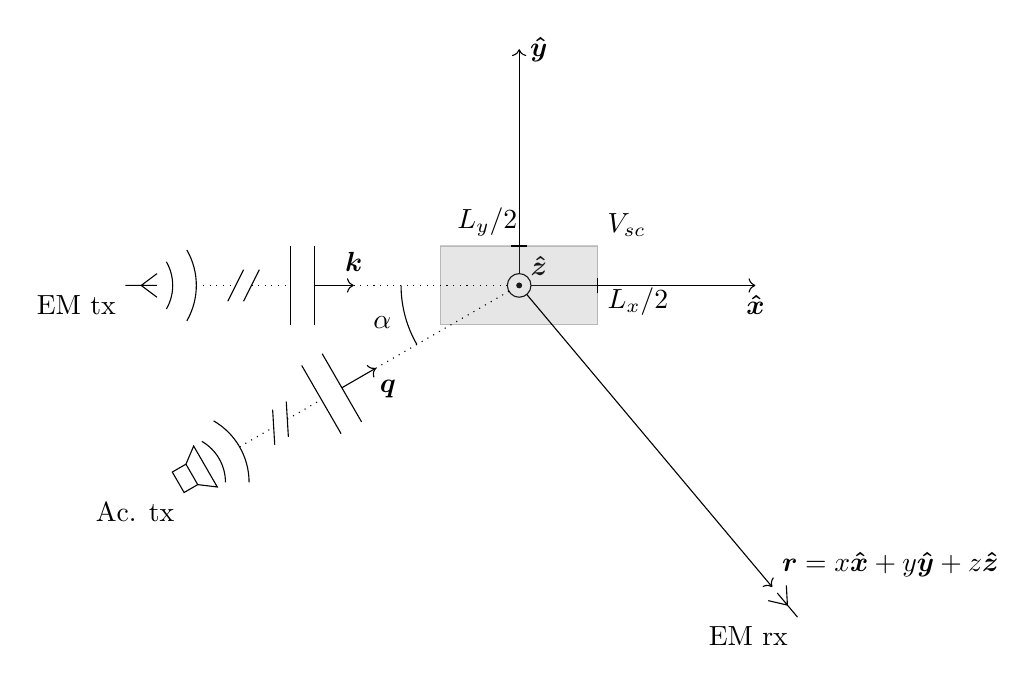
\begin{tikzpicture}
			% Draw coordinate axes
			\draw (0,0) circle(0.15);
			\filldraw[black] circle(0.03);
			\draw[->] (0.15,0) -- (3,0);
			\draw[->] (0,.150) -- (0,3);
			\draw (3,-0.25) node{$\bm{\hat{x}}$} (0.25,3) node{$\bm{\hat{y}}$} (0.25,0.25) node{$\bm{\hat{z}}$};
			
			% Draw scattering cube (or rectangle in this case)
			\draw[fill=gray,opacity=0.2] (-1,-0.5) rectangle(1,0.5);
			\draw (1,-0.1) -- (1,0.1) node[anchor= north west]{$L_{x}/2$} (-0.1,0.5) -- (0.1,0.5) node[anchor= south east]{$L_{y}/2$} (1,0.5) node[anchor=south west]{$V_\mrm{sc}$};
			
			% Draw EM tx and spherical waves
			\draw[shift = {(-5,0)}] (0,0) node[anchor=north east]{EM tx} -- (0.4,0) (0.2,0) -- (0.4,0.15)
			(0.2,0) -- (0.4,-0.15);
			\draw[shift = {(-5,0)}] ([shift={(-30:0.6)}] 0,0) arc(-30:30:0.6) ([shift={(-30:0.9)}] 0,0) arc(-30:30:0.9);
			
			% Draw EM "long distance" lines
			\draw[shift = {(-4.1,0)},dotted] (0,0) -- (0.5,0) (0.7,0) -- (1.2,0);
			\draw[shift = {(-4.1,0)}] (0.4,-0.2) -- (0.6,0.2) (0.6,-0.2) -- (0.8,0.2);
			
			% Draw EM plane waves
			\draw[shift = {(-2.9,0)}] (0,-0.5) -- (0,0.5) (0.3,-0.5) -- (0.3,0.5);
			\draw[shift = {(-2.6,0)}, ->] (0,0) -- (0.5,0);
			\draw[shift = {(-2.6,0)}] (0.5,0.3) node{$\bm{k}$};
			\draw[dotted] (-0.15,0) -- (-2.1,0);
			
			% Draw Ac. tx and spherical waves
			\draw[shift = {(210:5)}, rotate = 30] (0,-0.15) node[anchor=north east]{Ac. tx} rectangle (0.2,0.15) -- (0.4,0.3) -- (0.4,-0.3) -- (0.2,-0.15);
			\draw[shift = {(210:5)}, rotate = 30] ([shift={(-30:0.6)}] 0,0) arc(-30:30:0.6) ([shift={(-30:0.9)}] 0,0) arc(-30:30:0.9);
			
			% Draw Ac. "long distance" lines
			\draw[shift = {(210:4.1)}, rotate = 30,dotted] (0,0) -- (0.5,0) (0.7,0) -- (1.2,0);
			\draw[shift = {(210:4.1)}, rotate = 30] (0.4,-0.2) -- (0.6,0.2) (0.6,-0.2) -- (0.8,0.2);
			
			% Draw Ac. plane waves
			\draw[shift = {(210:2.9)}, rotate = 30] (0,-0.5) -- (0,0.5) (0.3,-0.5) -- (0.3,0.5);
			\draw[shift = {(210:2.6)}, rotate = 30, ->] (0,0) -- (0.5,0);
			\draw[shift = {(210:2.6)}, rotate = 30] (0.5,-0.3) node{$\bm{q}$};
			\draw[rotate = 30, dotted] (-0.15,0) -- (-2.1,0);
			
			% Draw angle alpha
			\draw ([shift={(180:1.5)}] 0,0) arc(180:210:1.5) (195:1.8) node{$\alpha$};
			
			% Draw line towards receiver
			\draw[->] (310:0.15) -- (310:5) node[anchor=south west]{$\bm{r} = x\bm{\hat{x}} + y\bm{\hat{y}} + z\bm{\hat{z}}$};
			
			% Draw EM rx
			\draw[shift = {(310:5.5)}, rotate = 130] (0,0) node[anchor=north east]{EM rx} -- (0.4,0) (0.2,0) -- (0.4,0.15) (0.2,0) -- (0.4,-0.15);
		\end{tikzpicture}
		}
		\caption{\label{fig:an-radar-geom} Geometry for the scattering problem.}
	\end{figure}
	The $xy$-plane is defined as the plane formed by the acoustic and electromagnetic wavevectors (they are assumed to be non-parallel). The scattering volume is a cuboid with dimensions $L_{x}$, $L_{y}$ and $L_{z}$. It is centered in the origin of the coordinate system, and both the acoustic and electromagnetic waves are approximated as plane waves close to the origin. Thus, the electromagnetic and dielectric perturbation fields near the origin are defined as
	\begin{align*}
		\bm{E}_\mrm{i} (\bm{r}',t) &= \bm{E}_\mrm{i} (\bm{r}') = \bm{E}_{\mrm{i}0} \eu^{\iu \bm{k}\cdot\bm{r}'} \\
		\varepsilon_1 (\bm{r}',t) &= \frac{\varepsilon_\mrm{r}^2 \mathfrak{p}}{K} p_0 \cos(\bm{q} \cdot \bm{r}' - \Omega t)
	\end{align*}
	Here, $\bm{E}_{\mrm{i}0}$ is the complex field amplitude at the origin ($-\iu\omega t$ time-dependence separated) and $\bm{k}$ is the electromagnetic wavevector. The scalar photoelastic relation from equation \eqref{eq:th-PE-scalar-p} has been used, where $\mathfrak{p}$ is the photoelastic constant, $p_0$ is the acoustic pressure amplitude at the origin, $K$ is the bulk modulus, $\bm{q}$ is the acoustic wavevector and $\Omega$ the acoustic frequency.
	
	The electromagnetic polarization is assumed to be in z, $\bm{E}_{\mrm{i}0} \parallel \bm{\hat{z}}$. For this problem, equation \eqref{eq:an-scatter-int} is written as (see appendix \ref{sec:app-derivations-radar-sol})
	\begin{equation*}
	\begin{split}
		\bm{E}_\mrm{sc}(\bm{r},t) =& \frac{\varepsilon_\mrm{r}k^2 \eu^{\iu kr} \bm{E}_{\mrm{i}0} \mathfrak{p} p_0}{8\pi r K} \\
		&\cdot \left( \eu^{-\iu \Omega t} \int_{V_\mrm{sc}} \eu^{\iu ( k(\bm{\hat{k}} - \bm{\hat{r}}) + \bm{q} ) \cdot \bm{r}'} \mathrm{d}v + \eu^{\iu \Omega t} \int_{V_\mrm{sc}} \eu^{\iu ( k(\bm{\hat{k}} - \bm{\hat{r}}) - \bm{q} ) \cdot \bm{r}'} \mathrm{d}v' \right)
	\end{split}
	\end{equation*}
	Given the geometry in figure \ref{fig:an-radar-geom}, the solution to this integral is written as (see appendix \ref{sec:app-derivations-radar-sol})
	\begin{equation*}
		\bm{E}_\mrm{sc} (\bm{r},t) = \bm{E}_{\mrm{i}0} \left( E_\mrm{A}^+ (\bm{r},t) + E_\mrm{A}^- (\bm{r},t) \right)
	\end{equation*}
	where
	\begin{equation*}
		E_\mrm{A}^\pm (\bm{r},t) = \frac{\varepsilon_\mrm{r}k^2 \eu^{\iu kr} \mathfrak{p} p_0}{8\pi r K} L_{x} L_{y} L_{z} e^{\mp \iu \Omega t} \Phi^\pm (\theta,\phi)
	\end{equation*}
	and
	\begin{equation*}
	\begin{split}
		\Phi^\pm(\theta,\phi) =& \text{sinc} \left( \frac{L_{x}}{2\pi} \left( k - k\sin{\theta}\cos{\phi} \pm q\cos{\alpha} \right) \right) \\
		\cdot& \text{sinc} \left( \frac{L_{y}}{2\pi} \left( -k\sin{\theta}\sin{\phi} \pm q\sin{\alpha} \right) \right) \\
		\cdot& \text{sinc} \left( -\frac{L_{z}}{2\pi} k\cos{\theta} \right)
	\end{split}
	\end{equation*}
	One important detail to note is that two distinct frequency components arise: one where the frequency is shifted up by $\Omega$ ($E_\mrm{A}^+$) and one where it is shifted down by $\Omega$ ($E_\mrm{A}^-$).
	
	To obtain a more practical expression, the equations are now transformed into power. For this, the time-averaged Poynting vector is calculated as (see appendix \ref{sec:app-derivations-radar-power})
	\begin{equation*}
		\left< \bm{S}_\mrm{sc}^\pm \right> (\bm{r}) = \frac{1}{2}\mathrm{Re}\left\{ \bm{E}_\mrm{sc}^\pm (\bm{r},t) \times \bm{H}_\mrm{sc}^{\pm*} (\bm{r},t) \right\} = \frac{\bm{\hat{r}}}{2\eta_0 \eta} |\bm{E}_{\mrm{i}0}|^2 |E_\mrm{A}^\pm (\bm{r},t)|^2
	\end{equation*}
	where $|E_\mrm{A}^\pm (\bm{r},t)|^2$ is given by
	\begin{equation*}
		|E_\mrm{A}^\pm (\bm{r},t)|^2 = \frac{\varepsilon_\mrm{r}^2 k^4 \mathfrak{p}^2 p_0^2}{64\pi^2 r^2 K^2} L_{x}^2 L_{y}^2 L_{z}^2 \Phi^\pm (\theta,\phi)^2
	\end{equation*}
	Using standard antenna parameters, the incident field can be written as (see appendix \ref{sec:app-derivations-radar-power})
	\begin{equation*}
		|\bm{E}_{\mrm{i}0}|^2 = 2\eta_0 \eta \frac{P_\mrm{T} G_\mrm{T}}{4\pi R_\mrm{T}^2}
	\end{equation*}
	where $P_\mrm{T}$ is the power accepted by the antenna, $G_\mrm{T}$ is the maximum gain of the antenna and $R_\mrm{T}$ is the distance from the antenna to the scattering center. This is inserted into the time-average of the power density, giving
	\begin{equation*}
		\left< \bm{S}_\mrm{sc}^\pm \right> (\bm{r}) = \bm{\hat{r}} \frac{P_\mrm{T} G_\mrm{T}}{4\pi R_\mrm{T}^2} \frac{\varepsilon_\mrm{r}^2 k^4 \mathfrak{p}^2 p_0^2}{64\pi^2 r^2 K^2} L_{x}^2 L_{y}^2 L_{z}^2 \Phi^\pm (\theta,\phi)^2
	\end{equation*}
	Now the effects of the receiving antenna are considered. It is assumed that this antenna is optimally directed towards the scattering center. The received power can then be written as (see appendix \ref{sec:app-derivations-radar-power})
	\begin{equation*}
		P_\mrm{R}^\pm = \frac{\lambda_\mrm{R}^2 G_\mrm{R}}{4\pi} \frac{P_\mrm{T} G_\mrm{T}}{4\pi R_\mrm{T}^2} \frac{\varepsilon_\mrm{r}^2 k^4 \mathfrak{p}^2 p_0^2}{64\pi^2 R_\mrm{R}^2 K^2} L_{x}^2 L_{y}^2 L_{z}^2 \Phi^\pm (\theta,\phi)^2
	\end{equation*}
	where $G_\mrm{R}$ is the gain of the receiving antenna, $\lambda_\mrm{R}$ the wavelength at the antenna (not necessarily the same as in the material) and $R_\mrm{R}$ the distance between the scattering center and the receiver. The receiver is located in the direction $(\theta,\phi)$ as seen from the scattering center. For a more traditional bistatic radar equation \cite{Richards2012} this can be written as
	\begin{equation*}
		P_\mrm{R}^\pm = \frac{P_\mrm{T} G_\mrm{T} G_\mrm{R} \lambda_\mrm{R}^2 \sigma^\pm (\theta,\phi)}{(4\pi)^3 R_\mrm{T}^2 R_\mrm{R}^2}
	\end{equation*}
	with the radar cross-section given by
	\begin{equation*}
		\sigma^\pm (\theta, \phi) = \frac{\varepsilon_\mrm{r}^2 k^4 \mathfrak{p}^2 p_0^2}{16\pi K^2} L_{x}^2 L_{y}^2 L_{z}^2 \Phi^\pm (\theta,\phi)^2
	\end{equation*}
	When actually measuring a signal, signal-to-noise ratio (SNR) is a more practical quantity than received power. The equation can be rewritten using SNR (see appendix \ref{sec:app-derivations-radar-SNR}) as:
	\begin{equation*}
		\mathit{SNR}^\pm_N = \frac{P_\mrm{T} G_\mrm{T} G_\mrm{R} \lambda_\mrm{R}^2 \sigma^\pm (\theta,\phi)}{(4\pi)^3 R_\mrm{T}^2 R_\mrm{R}^2 k_\mrm{B} T_0 B F} N
	\end{equation*}
	where $k_\mrm{B}$ is Boltzmann's constant, $T_0$ is the standard temperature 290 K, $B$ is the receiver bandwidth, $F$ is the noise ratio of the receiver and $N$ is the number of samples recorded. This equation assumes that coherent demodulation and integration is used to boost the SNR.
	
	Inspection of the equations for either scattered power or SNR shows that all angular dependence is contained in the function $\Phi^\pm$. This depends on the observation angles $\theta$, $\phi$ and the angle between EM and Ac. wavevectors $\alpha$. Conditions for the angles maximizing $\Phi^\pm$ are derived in appendix \ref{sec:app-derivations-bragg} and summarized as
	\begin{align}
		\theta &= \pi/2 \label{eq:an-bragg-theta} \\
		\cos{\alpha} = \mp \frac{q}{2k} &= \mp \frac{\lambda}{2\Lambda} \label{eq:an-bragg-alpha} \\
		\phi &= \mp \pi + 2\alpha \label{eq:an-bragg-phi}
	\end{align}
	The $\mp$-sign here is related to the $\pm$-sign indicating frequency shift of the scattered wave. These equations correspond directly to the Bragg condition used in acousto-optics (see appendix \ref{sec:app-derivations-bragg}). This gives the model some validation since the acousto-optic Bragg condition is derived from a slightly different starting point, but for the same basic phenomenon \cite{Saleh2007}.
	
	\todoint[inline]{Describe how ``maximum scattering'' is only relevant for one point $(\theta, \phi, \alpha)$. If power is measured on a surface (for example an antenna), the $\Phi$ function must be integrated, and the maximum for the integral must be found. This is cumbersome to do analytically, but through numerical integration and plotting it can be done.}
	
	\subsection{Refined interaction region}
	The analytical results presented above are based on a cuboid interaction region. This makes for simple calculations and is fairly straight-forward at a conceptual level. However, it is difficult to find good dimensions $L_x$, $L_y$, $L_z$ based on a real-life system using electromagnetic antennas and ultrasonic transducers. For this reason, the interaction region was refined for simple adaptation to real-life parameters. Other idealizations such as plane waves were still kept. The interaction region was now based on ''infinitely sharp´´ beams, meaning that fields behave as plane waves inside of the beam diameter and are zero outside. Two crossing beams form a parallelogram as shown in figure \ref{fig:an-parallelogram}.
	\begin{figure}[h]
		\centering
		\resizebox{\textwidth}{!}{
			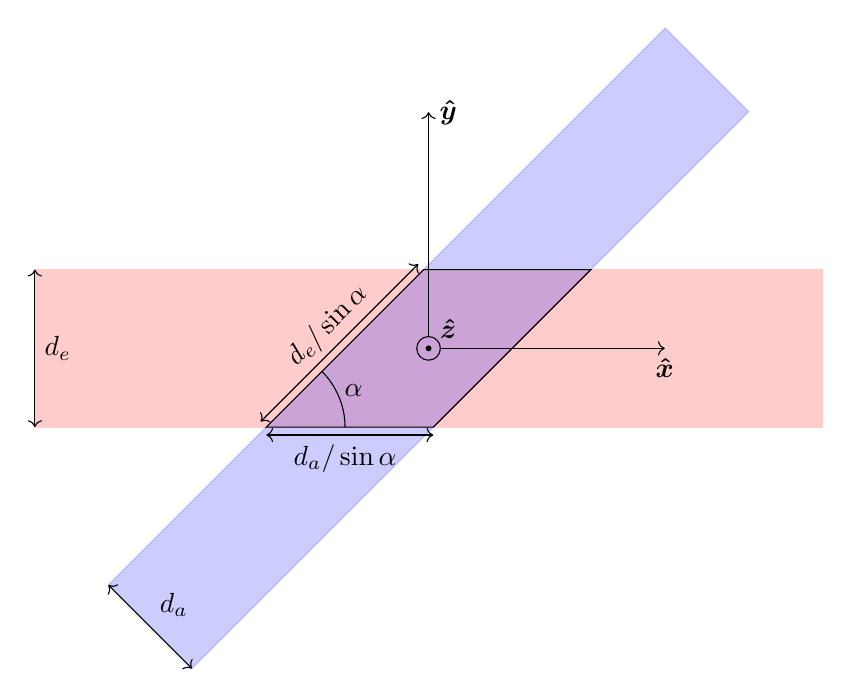
\begin{tikzpicture}
	
	
	% Draw EM beam
	\filldraw[red,opacity=0.2] (-5,-1) rectangle(5,1);
	\draw[<->] (-5,-1) -- (-5,1);
	\draw (-5,0) node[anchor=west]{$d_e$};
	
	% Draw Ac beam
	\filldraw[blue,rotate=45,opacity=0.2] (-5,-0.75) rectangle(5,0.75);
	\draw[<->,rotate=45] (-5,-0.75) -- (-5,0.75);
	\draw[rotate=45] (-5,0) node[anchor=south west]{$d_a$};
	
	% Draw parallelogram
	\draw (-2.061,-1) -- (-0.061,1) -- (2.061,1) -- (0.061,-1) -- cycle;
	\draw[<->] (-2.061,-1.1) -- (0.061, -1.1);
	\draw (-1.061, -1.4) node{$d_a/\sin{\alpha}$};
	\draw[<->, shift={(135:0.1)}] (-2.061,-1) -- (-0.061,1);
	\draw[shift={(135:0.4)}] (-1,0) node[anchor=center,rotate=45] {$d_e/\sin{\alpha}$};
	
	% Draw angle alpha
	\draw ([shift={(-1.061,-1)}] 0,0) arc(0:45:1) ([shift={(22.5:1.2)}] -2.061,-1) node{$\alpha$};
	
	% Draw coordinate axes
	\draw (0,0) circle(0.15);
	\filldraw[black] circle(0.03);
	\draw[->] (0.15,0) -- (3,0);
	\draw[->] (0,.150) -- (0,3);
	\draw (3,-0.25) node{$\bm{\hat{x}}$} (0.25,3) node{$\bm{\hat{y}}$} (0.25,0.25) node{$\bm{\hat{z}}$};
	
\end{tikzpicture}
		}
		\caption{\label{fig:an-parallelogram} Parallelogram interaction region. Electromagnetic beam diameter $d_\mrm{e}$, acoustic beam diameter $d_\mrm{a}$, angle between wave vectors $\alpha$.}
	\end{figure}
	This new interaction region alters the derivation somewhat in that the scattering integral \eqref{eq:an-scatter-int} is calculated over another region. The resulting scattered field is given by (see appendix \ref{sec:app-derivations-refined})
	\begin{equation*}
	\bm{E}_\mrm{sc,p} (\bm{r},t) = \bm{E}_{\mrm{i}0} \left( E_\mrm{A,p}^+ (\bm{r},t) + E_\mrm{A,p}^- (\bm{r},t) \right)
	\end{equation*}
	where
	\begin{equation*}
	E_\mrm{A,p}^\pm (\bm{r},t) = \frac{\varepsilon_\mrm{r}k^2 \eu^{\iu kr} \mathfrak{p} p_0}{8\pi r K} \frac{d_\mrm{a} d_\mrm{e} L_{z}}{\sin{\alpha}} e^{\mp \iu \Omega t} \Phi_\mrm{p}^\pm (\theta,\phi)
	\end{equation*}
	and
	\begin{equation*}
	\begin{split}
	\Phi_\mrm{p}^\pm =& \text{sinc}\left( \frac{d_\mrm{a}}{2\pi \sin{\alpha}}(k - k\sin{\theta}\cos{\phi} \pm q\cos{\alpha}) \right) \\
	&\cdot \text{sinc}\left( \frac{d_\mrm{e}}{2\pi \tan{\alpha}}
	(k - k\sin{\theta}(\cos{\phi} + \sin{\phi}\tan{\alpha}) \pm q(\cos{\alpha} + \sin{\alpha}\tan{\alpha})) \right) \\
	&\cdot \text{sinc}\left( -\frac{L_{z}}{2\pi} k\cos{\theta} \right)
	\end{split}
	\end{equation*}
	This is quite similar to the cuboid result, with the differences being in the interaction volume factor $d_\mrm{a} d_\mrm{e} L_{z}/\sin{\alpha}$ instead of $L_x L_y L_z$ in $E_\mrm{A}$ and the function for angular dependence $\Phi^\pm$. This result is easily transferable to power and SNR quantities. It can be shown (see appendix \ref{sec:app-derivations-bragg-refined}) that the same conditions for maximum scattering hold for this refined interaction region as for the cuboid interaction region, i.e. equations \eqref{eq:an-bragg-theta}, \eqref{eq:an-bragg-alpha} and \eqref{eq:an-bragg-phi}.
	\todoext{Write explicit equations for power and SNR}
	
	\chapter{Numerical Simulation}
	
	\section{Overview}
	The problem was simulated in COMSOL Multiphysics for verification and further investigation of more complex scenarios than the one modeled analytically. The two physics interfaces used were the ``Pressure Acoustics, Frequency Domain'' from the basic COMSOL Multiphysics and ``Electromagnetic Waves, Frequency Domain'' from the RF Module. Models were built in 2D for computational speed. One simulation required 1 acoustic and 2 electromagnetic frequency domain simulations to be run, and parameter sweeps would multiply the number required. It was decided that 3D simulations would be too time consuming with little gain when compared with 2D. \todoint{Details on 2D analytical model to compare with (and not 3D)}
	
	The pressure acoustics model was used even though propagation in a solid medium was to be modeled. This was done under an assumption of pure p-wave propagation, which can be modeled using acoustic pressure with a different wave speed as shown in section \ref{sec:th-prop-solid}. However, in these simulations the wave speed was calculated using the acoustic wave speed $v = \sqrt{K/\rho_0}$ which is only correct for p-waves in materials with negligible shear modulus \cite{Schmerr2016}. The reason for this was that wave speed and density entered the COMSOL physics model at multiple places such as the boundary conditions which made it more difficult to determine exactly how to change the wave speed without affecting other parameters. \todoint{Look into this more!}
	
	For all simulations the acoustic frequency was set to 450 MHz, which was used in acoustic frequency domain simulations. From this value and material properties, the acoustic wavelength $\Lambda$ was determined. Using the desired angle $\alpha$ between beams and equation \eqref{eq:an-bragg-alpha}, the electromagnetic wavelength $\lambda$ was calculated. From $\lambda$ and material properties the electromagnetic frequency was calculated, which was used in electromagnetic frequency domain simulations. For the material and angle mostly used, the electromagnetic frequency was approximately 61.29 GHz.
	
	\todoint[inline]{Describe why the frequency shift is not visible, and why this is not possible with the particular simulations used}
	
	\subsection{Geometry and boundary conditions}
	The basic geometry is shown in figure \ref{fig:sim-geometry} for the acoustic and electromagnetic simulations. The only difference in geometry between the two is the Perfectly Matched Layer (PML) which is used in the electromagnetic simulation but not the acoustic simulation. Additionally, the boundary conditions are different for the two simulations which is also shown. One boundary of special interest is the ``Measurement boundary''. This is where the physics domain ends, and the fields were measured at this boundary for post-processing. The radius of the measurement boundary was $30\Lambda$ everywhere except for the apertures which were chords of this circle.
	
	The PML was used to emulate an open boundary at the measurement boundary for the electromagnetic problem. It was a cylindrical type with center in the center of the geometry and a width of $2\lambda$. It used polynomial coordinate stretching with a typical wavelength taken from the electromagnetic physics interface. The PML scaling factor and PML scaling curvature parameter were both set to 1. At the exterior boundary, a Perfect Electric Conductor (PEC) boundary condition was used.
	
	The PML function was not available for the basic pressure acoustics interface used here. However, the Cylindrical Wave Radiation boundary condition was available and was used for the same purpose as a PML.
	
	\begin{figure}
		\centering
		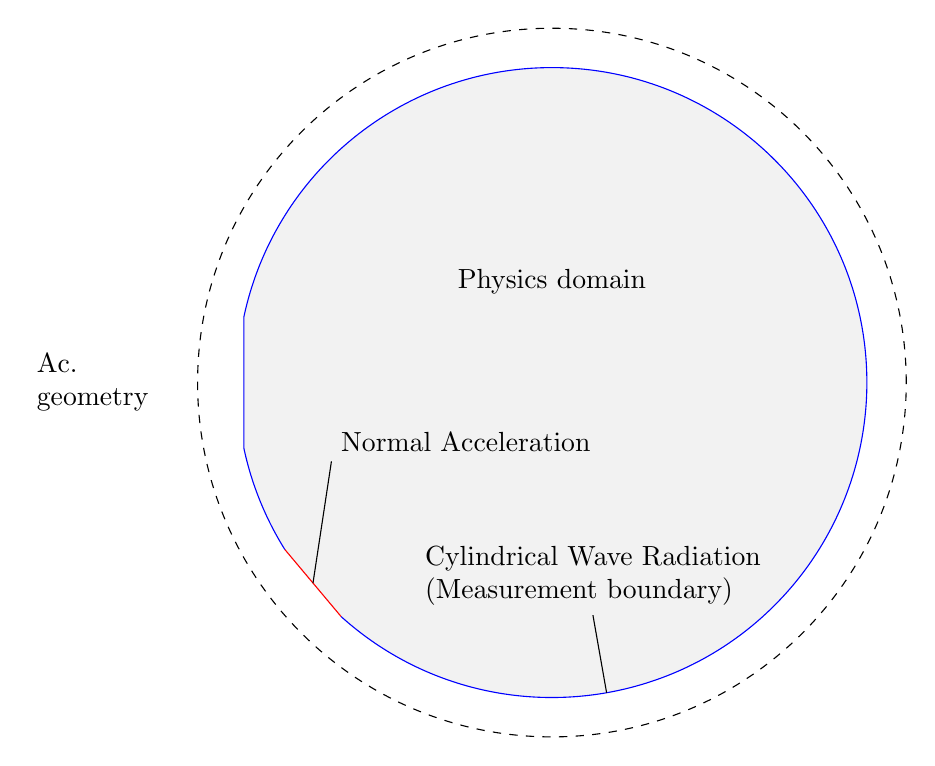
\begin{tikzpicture}
	
	% Fill domain
	\fill[gray!10] (0:4) arc(0:180-12:4) -- (180+12:4) arc(180+12:220-8:4) -- (220+8:4) arc(220+8:360:4);
	
	% Draw port
	\draw[red] (220-8:4) -- (220+8:4);
	
	% Draw inner boundary
	\draw[blue] (0:4) arc(0:180-12:4) -- (180+12:4) arc(180+12:220-8:4) (220+8:4) arc(220+8:360:4);
	
	% Draw outer boundary
	\draw[dashed] (0,0) circle(4.5);
	
	% Label domains
	\draw (0,1) node[anchor=south] {Physics domain};
	
	% Label boundaries
	\draw (220:{4*cos(8)}) -- (-2.8,-1) node[anchor=south west] {Normal Acceleration};
	\draw (280:4) -- (280:3) node[anchor=south, align=left] {Cylindrical Wave Radiation\\(Measurement boundary)};
	
	% Ac label
	\draw (180:5) node[anchor=east, align=left] {Ac.\\geometry};
	
\end{tikzpicture}
		\vspace{5 mm}
		
		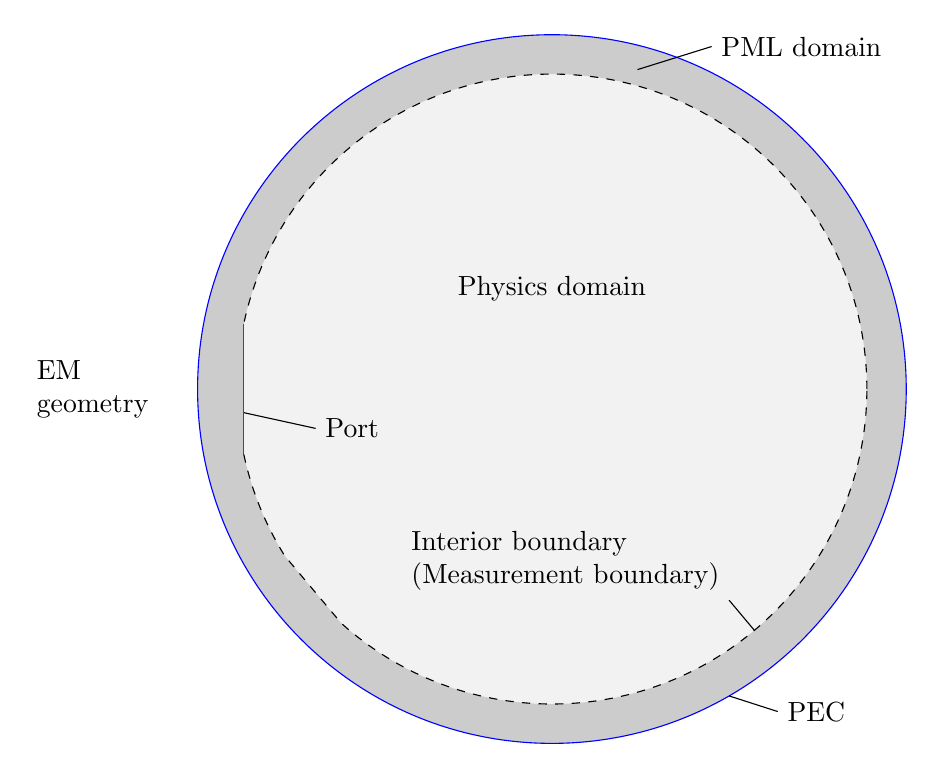
\begin{tikzpicture}
	
	% Fill domain
	\fill[gray!10] (0:4) arc(0:180-12:4) -- (180+12:4) arc(180+12:220-8:4) -- (220+8:4) arc(220+8:360:4);
	
	% Draw PML
	\fill[fill=gray!40, even odd rule] (0,0) circle(4.5) (0:4) arc(0:180-12:4) -- (180+12:4) arc(180+12:220-8:4) -- (220+8:4) arc(220+8:360:4);
	
	% Draw port
	\draw[red] (180-12:4) -- (180+12:4);
	
	% Draw inner boundary
	\draw[dashed] (0:4) arc(0:180-12:4) (180+12:4) arc(180+12:220-8:4) -- (220+8:4) arc(220+8:360:4);
	
	% Draw outer boundary
	\draw[blue] (0,0) circle(4.5);
	
	% Label domains
	\draw (0,1) node[anchor=south] {Physics domain};
	\draw (75:4.2) -- (65:4.8) node[anchor=west] {PML domain};
	
	% Label boundaries
	\draw (-60:4.5) -- (-55:5) node[anchor=west, align=left] {PEC};
	\draw (-{4*cos(12)},-0.3) -- (-3,-0.5) node[anchor=west] {Port};
	\draw (310:4) -- (310:3.5) node[anchor=south east, align=left] {Interior boundary\\(Measurement boundary)};
	
	% EM label
	\draw (180:5) node[anchor=east, align=left] {EM\\geometry};
	
\end{tikzpicture}
		\caption{\label{fig:sim-geometry} Simulation geometry with boundary conditions for Ac. and EM simulations.}
	\end{figure}
	
	\subsection{Tapering of apertures}
	To reduce sidelobe levels, both the electromagnetic and acoustic apertures had amplitude tapers applied to them. \addref This had the effect of lowering the electric field or acoustic acceleration near the edges of apertures. The specific taper used was a Gaussian taper, which multiplies values at the aperture with a Gaussian function given by
	\begin{equation*}
	\eu^{-(Ay')^2}
	\end{equation*}
	where $A$ affects the width of the taper and $y'$ is a coordinate along the aperture with 0 in the center. Since the model was based on a circle and all apertures were modeled as straight lines on the edge of the circle, $y'$ can be found by rotation of the original coordinate $y$ by the angle $\phi$. This transformation is given by \addref
	\begin{equation*}
		\begin{bmatrix}
			x' \\
			y'
		\end{bmatrix}
		=
		\begin{bmatrix}
			\cos{\phi} & \sin{\phi} \\
			-\sin{\phi} & \cos{\phi}
		\end{bmatrix}
		\begin{bmatrix}
			x \\
			y
		\end{bmatrix}
	\end{equation*}
	which gives the equation for $y'$
	\begin{equation*}
		y' = -x\sin{\phi} + y\cos{\phi}
	\end{equation*}
	The geometry is the same as previously shown in figure \ref{fig:an-radar-geom}. As such, $\phi = \pi$ for EM and $\phi = \pi + \alpha$ for Ac. For the coefficient $A$, it was found that $A = 4/D$ gave a good taper for an aperture width $D$.
	
	\subsection{Modeling of Electromagnetic Aperture}
	An electromagnetic aperture was designed to produce a fairly low beam width while not taking up too much space on the boundary. The model used a ``Port'' boundary condition on a boundary segment with length $D = 8\lambda$. The port options ``User Defined'' and wave excitation were turned on. The port input power was set to 15 dBm. Due to it being located on an interior boundary, the slit condition was activated with a domain-backed slit. For the port mode, the electric field was set as the input quantity with a tapered field in z defined as
	\begin{equation*}
		E_{0z} = e^{-(4y/D)^2}
	\end{equation*}
	where $y$ is a coordinate. The propagation constant was set to the wave number in the material using ``emw.k''.
	
	\subsection{Modeling of Acoustic Aperture}
	The qualities of beam width and space usage for the electromagnetic aperture were also taken into consideration in the design of the acoustic aperture. The model used a ``Normal Acceleration'' boundary condition on a boundary segment with length $D = 8\Lambda$. The acceleration was set to ``Inward acceleration''. The value of the acceleration amplitude was calculated from a displacement amplitude $u_\mrm{p}$ using $a_0 = \Omega^2 u_\mrm{p}$ \addref. The displacement amplitude was set to 5 nm \todo{Why? Show some reasonable order of magnitude}. The acceleration was tapered as
	\begin{equation*}
		a_\mrm{n} = a_0 \eu^{-(4(x\sin{\alpha} - y\cos{\alpha})/D)^2}
	\end{equation*}
	where $x$ and $y$ are coordinates and $\alpha$ the angle between wave vectors.
	
	\subsection{Photoelasticity model}
	To model photoelasticity in COMSOL, equation \eqref{eq:th-PE-scalar-p} was used with the photoelastic constant defined by equation \eqref{eq:th-PE-liquid-model}.
	
	\subsection{Material}
	The material model used was based on a foam core. The reason for this was that foam material is fairly homogeneous and isotropic (compared to honeycombs) and is used in aerospace applications \addref. The specific core selected was Divinycell HT251 from Diab Group, which is an aerospace core with applications described as ``Primary structures, radomes, control surfaces and interior components'' \cite{Diab2016}. The relevant material properties were density ($\rho_0$), bulk modulus ($K$) and relative permittivity ($\varepsilon_\mrm{r}$). These were $\rho_0 = 250$ kg/m$^3$, $K = 400$ MPa (nominal) and $\varepsilon_\mrm{r} = 1.29$ \cite{Diab2016}. In COMSOL, the required properties were density, speed of sound, relative permittivity, relative permeability and electric conductivity \todoint{More properties?}. The speed of sound was calculated using $v = \sqrt{K/\rho_0}$ \todoint{reference equation}, the relative permeability was set to 1 and the conductivity to 0. The assumption was that the material was perfectly non-conducting and non-magnetic.
	
	\subsection{Mesh}
	Two meshes were used in simulations: one for the acoustic simulation and one for the electromagnetic simulation. The reason for this was primarily the difference in wavelength.
	
	The acoustic mesh was defined on both the physics domain and PML domain even though only the physics domain was simulated in this case. A free triangular mesh was used with element size between $\Lambda/10$ and $\Lambda/10 \cdot 3 \cdot 10^{-2}$ in the physics domain, and ``Fine'' in the PML domain. Before running the free triangular meshing, the mesh was defined on the measurement boundary.
	
	The electromagnetic mesh used a free triangular mesh in the physics domain and a mapped mesh in the PML domain. The element size in the physics domain was between $\lambda/10$ and $\lambda/10 \cdot 3 \cdot 10^{-2}$. Before running the free triangular meshing, the mesh was defined on the measurement boundary.
	
	\subsection{Simulation studies}
	Before starting simulations, the frequencies, material and geometry were defined. The geometry was in many parts defined as a function of the frequencies and material properties in order to obtain reasonably sized domains and apertures placed according to the Bragg condition.
	
	For the actual simulations, the work flow is illustrated in figure \ref{fig:simulationflow}. First, an acoustic frequency domain study was run using the acoustic frequency and mesh. The result from this was a complex pressure field. Real part convention was used when relating this complex field to the actual pressure.
	
	To transform the pressure to relative permittivity, a variable was used in the material model to define the relative permittivity. This variable took the real part of the pressure field as its input, and used equations \eqref{eq:th-PE-scalar} and \eqref{eq:th-PE-scalar-p} to calculate a corresponding field for $\varepsilon_1$.
	
	An electromagnetic frequency domain study was now run using the electromagnetic frequency and mesh. The acoustic study was used for calculating initial values for variables not solved for. This was necessary for the pressure field to be available in both studies. Since the photoelastic effect is usually very small, the scattered field was not possible to distinguish with the incident field present. To be able to isolate the scattered field, two simulations were run: one where the relative permittivity of the material was unperturbed and one where it was perturbed by $\varepsilon_1$. The difference between fields resulting from these simulations were identified as the scattered fields.
	
	Due to limitations in the post-processing capabilities of COMSOL, the $E_z$, $H_x$ and $H_y$ fields at the boundary were exported together with $x$ and $y$ coordinates after the electromagnetic simulation was finished. This was done both for the simulation with and without perturbation.
	
	\begin{figure}[h]
		\centering
		\resizebox{\textwidth}{!}{
			
% http://www.texample.net/tikz/examples/simple-flow-chart/
\tikzstyle{sim} = [rectangle, draw, fill=blue!20, 
text width=5em, text centered, rounded corners, minimum height=4em]
\tikzstyle{res} = [draw, ellipse,fill=red!20]

\begin{tikzpicture}[node distance = 2 cm, auto]

	\draw[dashed] (-2,1) rectangle(2,-7);
	\node[anchor=south west, text width=10em] at (-2,1) {Pressure acoustics, frequency domain};
	
	\node[sim] at (0,0) (Ac) {Ac. Simulation};
	\node[res, below of=Ac] (p) {$p$ field};
	\node[sim, below of=p] (real) {Calculation on real part};
	\node[res, below of=real] (er) {$\varepsilon_1$ field};
	
	\draw[->] (Ac) -- (p);
	\draw[->] (p) -- (real);
	\draw[->] (real) -- (er);
	
	\draw[dashed] (4,1) rectangle(12,-3);
	\node[anchor=south west, text width=11em] at (4,1) {Electromagnetic waves, frequency domain};
	
	\node[sim] at (6,0) (EM1) {EM Simulation w/o PE};
	\node[res, below of=EM1] (emw1) {$\bm{E}_i$, $\bm{H}_i$ fields};
	\node[sim] at (10,0) (EM2) {EM Simulation w/ PE};
	\node[res, below of=EM2] (emw2) {$\bm{E}$, $\bm{H}$ fields};
	
	\draw[->] (EM1) -- (emw1);
	\draw[->] (EM2) -- (emw2);
	
	\draw[->] (er.east) -- (3,-6) -- (3,2.5) -- (10,2.5) -- (EM2.north);
	
	\node[sim] at (8,-4) (diff) {Difference};
	\node[res, below of=diff] (sc) {$\bm{E}_{sc}$, $\bm{H}_{sc}$ fields};
	\draw[->] (emw1.south) -- (6,-4) -- (diff.west);
	\draw[->] (emw2.south) -- (10,-4) -- (diff.east);
	\draw[->] (diff.south) -- (sc.north);
	
\end{tikzpicture}
		}
		\caption{\label{fig:simulationflow} Simulation flow chart}
	\end{figure}
	
	\subsection{Post-processing}
	The simulation results were further processed in SciPy for better visualization of the results than what was possible in COMSOL. The $E_z$, $H_x$ and $H_y$ fields (both with and without photoelastic perturbation) on the domain boundary were exported from COMSOL and loaded in SciPy. The differences between the fields were calculated to obtain the scattered fields. The time-averaged Poynting vector (for scattered fields) was then calculated as
	\begin{align*}
	\left< S_{\mrm{sc},x} \right> &= -\frac{1}{2} \text{Re} \{ E_{\mrm{sc},z} H_{\mrm{sc},y}^* \} \\
	\left< S_{\mrm{sc},y} \right> &= \frac{1}{2} \text{Re} \{ E_{\mrm{sc},z} H_{\mrm{sc},x}^* \}
	\end{align*}
	Due to it being easier to visualize, the magnitude of the time-averaged Poynting vector was also calculated. Using the $x$ and $y$ coordinates, the observation angle $\phi_\mrm{obs}$ for each point was calculated and the data was sorted according to this. A measure for the total scattered power was calculated by integrating the magnitude of the time-averaged Poynting vector over the entire boundary. This was done using the trapezoidal method with the distances between points calculated from the coordinates.
	
	One thing to note is that the definition for radiated power is \todoint{Define this in a good way (2D) and cite something}
	\begin{equation*}
		\int_{C_\mrm{mb}} \left< \bm{S} \right> \cdot \bm{\hat{n}} \, \mrm{d}l
	\end{equation*}
	where $\bm{\hat{n}}$ is the normal to the measurement boundary $C_\mrm{mb}$. However, here the calculation was instead
	\begin{equation*}
		\int_{C_\mrm{mb}} \left| \left< \bm{S} \right> \right|  \, \mrm{d}l
	\end{equation*}
	The reason behind this is that the boundary curvature was large when compared with the beams of interest. This would cause scattered field originating away from the center of the geometry to have less influence on the measure for total scattered power. This can be seen in figure \ref{fig:sim-postproc-angles} where the propagation angle, $\phi_\mrm{prop}$, differs from the observation angle normal to the boundary, $\phi_\mrm{obs}$, for much of the scattered field. Using the magnitude of the Poynting vector instead decreases the influence of the boundary geometry.
	
	For plotting of the time-averaged Poynting vector magnitude, the propagation angle $\phi_\mrm{prop}$ was calculated for each data point. The two angles $\phi_\mrm{obs}$ and $\phi_\mrm{prop}$ are shown in figure \ref{fig:sim-postproc-angles} together with the geometry of the problem. From this figure it can be seen that the observation angle depends highly on the measurement point while the propagation angle is a property of the scattered field. For this reason, the propagation angle was chosen for use in plots where the angle mattered.
	
	\begin{figure}[h]
		\centering
		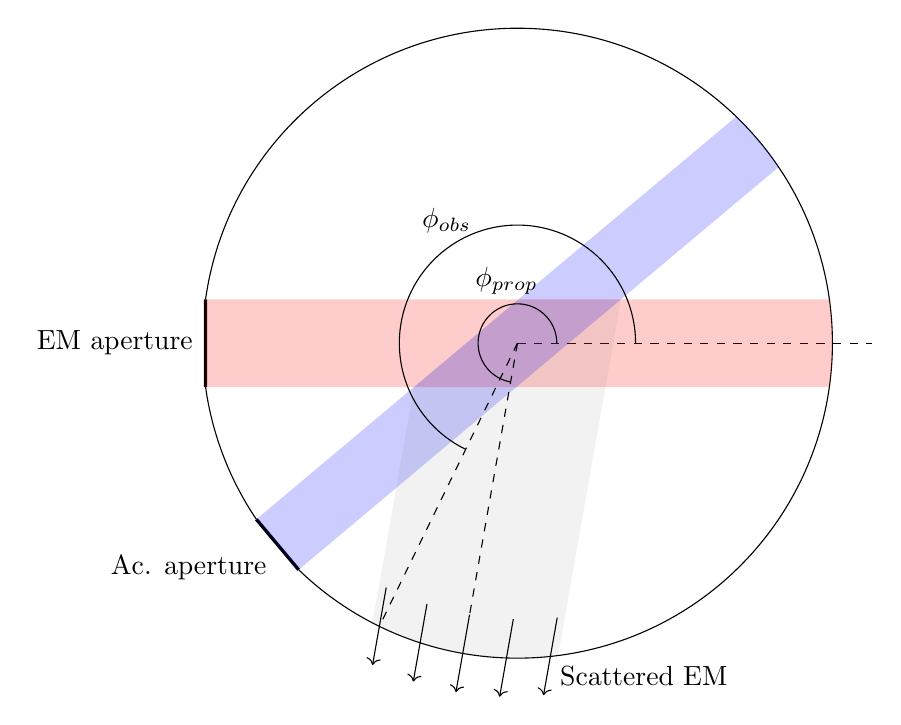
\begin{tikzpicture}
	% Draw coordinate lines (dashed)
	\draw[dashed] (0,0) -- (4.5,0);
	
	% Draw boundary
	\draw (0:4) arc(0:172:4) (188:4) arc(188:214:4) (226:4) arc(226:360:4);
	\draw[very thick] (172:4) -- (188:4) (214:4) -- (226:4);
	
	% Draw incident beams
	\fill[red,opacity=0.2] (172:4) -- (8:4) arc(8:-8:4) -- (188:4) -- cycle;
	\fill[blue,opacity=0.2] (214:4) -- (46:4) arc(46:34:4) -- (226:4) -- cycle;
	
	% Find intersections for interaction region definition
	\draw (172:4) coordinate(em1a) (8:4) coordinate(em1b) (188:4) coordinate(em2a) (-8:4) coordinate(em2b);
	\draw (214:4) coordinate(ac1a) (46:4) coordinate(ac1b) (226:4) coordinate(ac2a) (34:4) coordinate(ac2b);
	\coordinate (c1) at (intersection of em2a--em2b and ac1a--ac1b);
	\coordinate (c2) at (intersection of em1a--em1b and ac1a--ac1b);
	\coordinate (c3) at (intersection of em1a--em1b and ac2a--ac2b);
	
	% Draw scattered beam
	\begin{scope}
		\clip (0,0) circle(4);
		\fill[gray,opacity=0.1] (c1) -- (c2) -- (c3) -- ([shift={(c3)}] 260:6) -- ([shift={(c1)}] 260:6) -- cycle;
	\end{scope}
	
	% Draw field vectors
	\draw[->, shift={(260:4)}, rotate=260] (-0.5,0) -- (0.5,0);
	\draw[->, shift={(268:4)}, rotate=260] (-0.5,0) -- (0.5,0);
	\draw[->, shift={(276:4)}, rotate=260] (-0.5,0) -- (0.5,0);
	\draw[->, shift={(252:4)}, rotate=260] (-0.5,0) -- (0.5,0);
	\draw[->, shift={(244:4)}, rotate=260] (-0.5,0) -- (0.5,0);
	
	% Draw lines from origin to vectors
	\draw[dashed] (260:0) -- (260:3.5);
	\draw[dashed] (0,0) -- ([shift={(244:4)}, rotate=260] 0,0);
	
	% Draw angles
	\draw ([shift={(0:0.5)}] 0,0) arc(0:260:0.5) (100:0.8) node{$\phi_\mrm{prop}$};
	\draw ([shift={(0:1.5)}] 0,0) arc(0:244:1.5) (120:1.8) node{$\phi_\mrm{obs}$};
	
	% Descriptions for beams
	\draw (180:4) node[anchor=east] {EM aperture};
	\draw (220:4) node[anchor=north east] {Ac. aperture};
	\draw (276:4) node[anchor=north west] {Scattered EM};
	
\end{tikzpicture}
		\caption{\label{fig:sim-postproc-angles} Propagation and observation angle near the edge of the scattered beam.}
	\end{figure}
		
	\section{Comparison with Analytical Model - Angles}
	To compare with the results from section \ref{sec:analytical-radar} the frequencies of the acoustic and electromagnetic waves were matched to a Bragg angle of $40^\circ$ while the angle $\alpha$ between the wavevectors was swept between $\pm 5^\circ$ of the optimal angle. This was done both for (+) and (-) scattering by sweeping around either $\alpha = 40^\circ$ or $\alpha = 140^\circ$, as these angles are the ones given by equation \eqref{eq:an-bragg-alpha} as angles for maximum scattering.
	
	\section{Comparision with Analytical Model - Power}
	\todoext{Not correct, 2D version of the derivations should be done to compare with COMSOL results}
	To compare the power measure with the analytical calculation, the integral of the Poynting vector was calculated using the theoretical value for both cuboid and parallelogram interaction regions (see appendix \ref{sec:app-derivations-radar}).
	\begin{align*}
	P_\mrm{cub} &= \int_{C_\mrm{mb}} \left| \left< \bm{S}_\mrm{sc}^\pm \right> \right| \mrm{d}l
	= \frac{P_\mrm{T} G_\mrm{T}}{4\pi R_\mrm{T}^2} \frac{\varepsilon_\mrm{r}^2 k^4}{64 \pi^2 r^2} \mathfrak{p}^2 S_0^2 L_{x}^2 L_{y}^2 L_{z}^2 \int_{C_\mrm{mb}} \Phi^\pm (\theta,\phi)^2 \mrm{d}l \\
	P_\mrm{par} &= \int_{C_\mrm{mb}} \left| \left< \bm{S}_\mrm{sc}^\pm \right> \right| \mrm{d}l
	= \frac{P_\mrm{T} G_\mrm{T}}{4\pi R_\mrm{T}^2} \frac{\varepsilon_\mrm{r}^2 k^4}{64 \pi^2 r^2} \mathfrak{p}^2 S_0^2 \frac{d_\mrm{a}^2 d_\mrm{e}^2 L_z^2}{\sin^2{\alpha}} \int_{C_\mrm{mb}} \Phi_\mrm{p}^\pm (\theta,\phi)^2 \mrm{d}l
	\end{align*}
	where the indices cub and par denote cuboid and parallelogram interaction regions. $\Phi$ and $\Phi_\mrm{p}$ are given by equation. \todoint{refer to correct equations from before} The integrals were calculated numerically using the trapezoid method. The measurement boundary was then approximated by a circle with the radius $30\Lambda$, which was also the value for $R_\mrm{T}$ and $r$. $S_0$ was calculated using the peak acoustic pressure close to the origin from COMSOL \todoint{equation for pressure stuff}. The geometry variables $L_x$, $L_y$, $d_\mrm{a}$ and $d_\mrm{e}$ were estimated from the center of the interaction region in the COMSOL simulation.
	To obtain $G_\mrm{T}$, the beamwidth $\Delta \theta_B$ of the electromagnetic beam was estimated. With an assumption of small beamwidth and lossless antenna it holds that \cite{Orfanidis2016}
	\begin{equation*}
	G_\mrm{T} = D_\mrm{max} = \frac{16}{(\Delta \theta_B)^2}
	\end{equation*}
	where $D_\mrm{max}$ is the peak directivity and the beamwidth is for the full beam \cite{Orfanidis2016}.
	
	\section{Conductive Defect}
	To examine the effect of a defect with electromagnetic contrast but no acoustic contrast, simulations were run with a conductive defect. The geometry of this problem was based on the basic geometry shown in figure \ref{fig:sim-geometry}. The addition was a circle in the center of the physics domain representing a defect. This had the diameter equal to the electromagnetic wavelength $\lambda$. The material in this region was the same as in the physics domain, but with a nonzero electric conductivity.
	
	To demonstrate the effect of conductivity, the electric conductivity of the defect was swept between 0 and 10 S/m in steps of 1 S/m. The angle $\alpha$ was fixed at $40^\circ$ with $\lambda$ matched to $\Lambda$ and this angle.
	
	\section{Mechanical Defect}
	To examine the effect of a defect with acoustic contrast but no electromagnetic contrast, simulations were run with a mechanical defect. The mechanical property which was altered was the density since this does not affect the photoelastic relation from equation \eqref{eq:th-PE-scalar-p} (for a constant bulk modulus). Since the bulk modulus was kept constant, the acoustic wave speed was changed as the density changed. The geometry of this problem was the same as for the conductive defect simulation. The material inside of the defect region was the same as in the physics domain, but with altered density.
	
	To demonstrate the effect of density change, the density was swept between 100 and 400 kg/m$^3$ in steps of 25 kg/m$^3$. The angle $\alpha$ was fixed at $40^\circ$ with $\lambda$ matched to $\Lambda$ and this angle.
	
	\chapter{Results and Discussion}
	
	\section{Numerical Simulation Results}
	
	\subsection{Comparison with Analytical Model - Angle}
	The results from the sweep of the angle $\alpha$ are shown in figures \ref{fig:res-angle-sweep-peak} - \ref{fig:res-angle-sweep-polar} for both the (+) and (-) scattering cases. Figure \ref{fig:res-angle-sweep-peak} shows the peak of the scattered Poynting vector magnitude due to photoelasticity for the angles $\alpha = 40^\circ \pm 5^\circ$. The values are normalized and compared with analytical values. Figure \ref{fig:res-angle-sweep-power} shows the total scattered power due to photoelasticity for the angles $\alpha = 40^\circ \pm 5^\circ$. Figure \ref{fig:res-angle-sweep-angles} shows the relationship between scattering angle $\phi$ (using the propagation angle $\phi_\mrm{prop}$) and angle between wave vectors $\alpha$. This was plotted using a weighted average of the propagation angle with weights of the Poynting vector corresponding to that angle. This way scattering angles which were not contributing much to the power (such as noise) had their effect on the final value greatly reduced. Figure \ref{fig:res-angle-sweep-polar} shows the magnitude of the Poynting vector for different propagation angles $\phi_\mrm{prop}$ as a polar plot. The values are normalized.
	
	\begin{figure}[h]
		\centering
		\begin{subfigure}{\textwidth}
			\resizebox{\textwidth}{!}{
				%% Creator: Matplotlib, PGF backend
%%
%% To include the figure in your LaTeX document, write
%%   \input{<filename>.pgf}
%%
%% Make sure the required packages are loaded in your preamble
%%   \usepackage{pgf}
%%
%% Figures using additional raster images can only be included by \input if
%% they are in the same directory as the main LaTeX file. For loading figures
%% from other directories you can use the `import` package
%%   \usepackage{import}
%% and then include the figures with
%%   \import{<path to file>}{<filename>.pgf}
%%
%% Matplotlib used the following preamble
%%   \usepackage{fontspec}
%%   \setmainfont{DejaVu Serif}
%%   \setsansfont{DejaVu Sans}
%%   \setmonofont{DejaVu Sans Mono}
%%
\begingroup%
\makeatletter%
\begin{pgfpicture}%
\pgfpathrectangle{\pgfpointorigin}{\pgfqpoint{6.400000in}{4.800000in}}%
\pgfusepath{use as bounding box, clip}%
\begin{pgfscope}%
\pgfsetbuttcap%
\pgfsetmiterjoin%
\definecolor{currentfill}{rgb}{1.000000,1.000000,1.000000}%
\pgfsetfillcolor{currentfill}%
\pgfsetlinewidth{0.000000pt}%
\definecolor{currentstroke}{rgb}{1.000000,1.000000,1.000000}%
\pgfsetstrokecolor{currentstroke}%
\pgfsetdash{}{0pt}%
\pgfpathmoveto{\pgfqpoint{0.000000in}{0.000000in}}%
\pgfpathlineto{\pgfqpoint{6.400000in}{0.000000in}}%
\pgfpathlineto{\pgfqpoint{6.400000in}{4.800000in}}%
\pgfpathlineto{\pgfqpoint{0.000000in}{4.800000in}}%
\pgfpathclose%
\pgfusepath{fill}%
\end{pgfscope}%
\begin{pgfscope}%
\pgfsetbuttcap%
\pgfsetmiterjoin%
\definecolor{currentfill}{rgb}{1.000000,1.000000,1.000000}%
\pgfsetfillcolor{currentfill}%
\pgfsetlinewidth{0.000000pt}%
\definecolor{currentstroke}{rgb}{0.000000,0.000000,0.000000}%
\pgfsetstrokecolor{currentstroke}%
\pgfsetstrokeopacity{0.000000}%
\pgfsetdash{}{0pt}%
\pgfpathmoveto{\pgfqpoint{0.800000in}{0.528000in}}%
\pgfpathlineto{\pgfqpoint{5.760000in}{0.528000in}}%
\pgfpathlineto{\pgfqpoint{5.760000in}{4.224000in}}%
\pgfpathlineto{\pgfqpoint{0.800000in}{4.224000in}}%
\pgfpathclose%
\pgfusepath{fill}%
\end{pgfscope}%
\begin{pgfscope}%
\pgfpathrectangle{\pgfqpoint{0.800000in}{0.528000in}}{\pgfqpoint{4.960000in}{3.696000in}} %
\pgfusepath{clip}%
\pgfsetrectcap%
\pgfsetroundjoin%
\pgfsetlinewidth{0.803000pt}%
\definecolor{currentstroke}{rgb}{0.690196,0.690196,0.690196}%
\pgfsetstrokecolor{currentstroke}%
\pgfsetdash{}{0pt}%
\pgfpathmoveto{\pgfqpoint{1.476364in}{0.528000in}}%
\pgfpathlineto{\pgfqpoint{1.476364in}{4.224000in}}%
\pgfusepath{stroke}%
\end{pgfscope}%
\begin{pgfscope}%
\pgfsetbuttcap%
\pgfsetroundjoin%
\definecolor{currentfill}{rgb}{0.000000,0.000000,0.000000}%
\pgfsetfillcolor{currentfill}%
\pgfsetlinewidth{0.803000pt}%
\definecolor{currentstroke}{rgb}{0.000000,0.000000,0.000000}%
\pgfsetstrokecolor{currentstroke}%
\pgfsetdash{}{0pt}%
\pgfsys@defobject{currentmarker}{\pgfqpoint{0.000000in}{-0.048611in}}{\pgfqpoint{0.000000in}{0.000000in}}{%
\pgfpathmoveto{\pgfqpoint{0.000000in}{0.000000in}}%
\pgfpathlineto{\pgfqpoint{0.000000in}{-0.048611in}}%
\pgfusepath{stroke,fill}%
}%
\begin{pgfscope}%
\pgfsys@transformshift{1.476364in}{0.528000in}%
\pgfsys@useobject{currentmarker}{}%
\end{pgfscope}%
\end{pgfscope}%
\begin{pgfscope}%
\pgftext[x=1.476364in,y=0.430778in,,top]{\sffamily\fontsize{10.000000}{12.000000}\selectfont 36}%
\end{pgfscope}%
\begin{pgfscope}%
\pgfpathrectangle{\pgfqpoint{0.800000in}{0.528000in}}{\pgfqpoint{4.960000in}{3.696000in}} %
\pgfusepath{clip}%
\pgfsetrectcap%
\pgfsetroundjoin%
\pgfsetlinewidth{0.803000pt}%
\definecolor{currentstroke}{rgb}{0.690196,0.690196,0.690196}%
\pgfsetstrokecolor{currentstroke}%
\pgfsetdash{}{0pt}%
\pgfpathmoveto{\pgfqpoint{2.378182in}{0.528000in}}%
\pgfpathlineto{\pgfqpoint{2.378182in}{4.224000in}}%
\pgfusepath{stroke}%
\end{pgfscope}%
\begin{pgfscope}%
\pgfsetbuttcap%
\pgfsetroundjoin%
\definecolor{currentfill}{rgb}{0.000000,0.000000,0.000000}%
\pgfsetfillcolor{currentfill}%
\pgfsetlinewidth{0.803000pt}%
\definecolor{currentstroke}{rgb}{0.000000,0.000000,0.000000}%
\pgfsetstrokecolor{currentstroke}%
\pgfsetdash{}{0pt}%
\pgfsys@defobject{currentmarker}{\pgfqpoint{0.000000in}{-0.048611in}}{\pgfqpoint{0.000000in}{0.000000in}}{%
\pgfpathmoveto{\pgfqpoint{0.000000in}{0.000000in}}%
\pgfpathlineto{\pgfqpoint{0.000000in}{-0.048611in}}%
\pgfusepath{stroke,fill}%
}%
\begin{pgfscope}%
\pgfsys@transformshift{2.378182in}{0.528000in}%
\pgfsys@useobject{currentmarker}{}%
\end{pgfscope}%
\end{pgfscope}%
\begin{pgfscope}%
\pgftext[x=2.378182in,y=0.430778in,,top]{\sffamily\fontsize{10.000000}{12.000000}\selectfont 38}%
\end{pgfscope}%
\begin{pgfscope}%
\pgfpathrectangle{\pgfqpoint{0.800000in}{0.528000in}}{\pgfqpoint{4.960000in}{3.696000in}} %
\pgfusepath{clip}%
\pgfsetrectcap%
\pgfsetroundjoin%
\pgfsetlinewidth{0.803000pt}%
\definecolor{currentstroke}{rgb}{0.690196,0.690196,0.690196}%
\pgfsetstrokecolor{currentstroke}%
\pgfsetdash{}{0pt}%
\pgfpathmoveto{\pgfqpoint{3.280000in}{0.528000in}}%
\pgfpathlineto{\pgfqpoint{3.280000in}{4.224000in}}%
\pgfusepath{stroke}%
\end{pgfscope}%
\begin{pgfscope}%
\pgfsetbuttcap%
\pgfsetroundjoin%
\definecolor{currentfill}{rgb}{0.000000,0.000000,0.000000}%
\pgfsetfillcolor{currentfill}%
\pgfsetlinewidth{0.803000pt}%
\definecolor{currentstroke}{rgb}{0.000000,0.000000,0.000000}%
\pgfsetstrokecolor{currentstroke}%
\pgfsetdash{}{0pt}%
\pgfsys@defobject{currentmarker}{\pgfqpoint{0.000000in}{-0.048611in}}{\pgfqpoint{0.000000in}{0.000000in}}{%
\pgfpathmoveto{\pgfqpoint{0.000000in}{0.000000in}}%
\pgfpathlineto{\pgfqpoint{0.000000in}{-0.048611in}}%
\pgfusepath{stroke,fill}%
}%
\begin{pgfscope}%
\pgfsys@transformshift{3.280000in}{0.528000in}%
\pgfsys@useobject{currentmarker}{}%
\end{pgfscope}%
\end{pgfscope}%
\begin{pgfscope}%
\pgftext[x=3.280000in,y=0.430778in,,top]{\sffamily\fontsize{10.000000}{12.000000}\selectfont 40}%
\end{pgfscope}%
\begin{pgfscope}%
\pgfpathrectangle{\pgfqpoint{0.800000in}{0.528000in}}{\pgfqpoint{4.960000in}{3.696000in}} %
\pgfusepath{clip}%
\pgfsetrectcap%
\pgfsetroundjoin%
\pgfsetlinewidth{0.803000pt}%
\definecolor{currentstroke}{rgb}{0.690196,0.690196,0.690196}%
\pgfsetstrokecolor{currentstroke}%
\pgfsetdash{}{0pt}%
\pgfpathmoveto{\pgfqpoint{4.181818in}{0.528000in}}%
\pgfpathlineto{\pgfqpoint{4.181818in}{4.224000in}}%
\pgfusepath{stroke}%
\end{pgfscope}%
\begin{pgfscope}%
\pgfsetbuttcap%
\pgfsetroundjoin%
\definecolor{currentfill}{rgb}{0.000000,0.000000,0.000000}%
\pgfsetfillcolor{currentfill}%
\pgfsetlinewidth{0.803000pt}%
\definecolor{currentstroke}{rgb}{0.000000,0.000000,0.000000}%
\pgfsetstrokecolor{currentstroke}%
\pgfsetdash{}{0pt}%
\pgfsys@defobject{currentmarker}{\pgfqpoint{0.000000in}{-0.048611in}}{\pgfqpoint{0.000000in}{0.000000in}}{%
\pgfpathmoveto{\pgfqpoint{0.000000in}{0.000000in}}%
\pgfpathlineto{\pgfqpoint{0.000000in}{-0.048611in}}%
\pgfusepath{stroke,fill}%
}%
\begin{pgfscope}%
\pgfsys@transformshift{4.181818in}{0.528000in}%
\pgfsys@useobject{currentmarker}{}%
\end{pgfscope}%
\end{pgfscope}%
\begin{pgfscope}%
\pgftext[x=4.181818in,y=0.430778in,,top]{\sffamily\fontsize{10.000000}{12.000000}\selectfont 42}%
\end{pgfscope}%
\begin{pgfscope}%
\pgfpathrectangle{\pgfqpoint{0.800000in}{0.528000in}}{\pgfqpoint{4.960000in}{3.696000in}} %
\pgfusepath{clip}%
\pgfsetrectcap%
\pgfsetroundjoin%
\pgfsetlinewidth{0.803000pt}%
\definecolor{currentstroke}{rgb}{0.690196,0.690196,0.690196}%
\pgfsetstrokecolor{currentstroke}%
\pgfsetdash{}{0pt}%
\pgfpathmoveto{\pgfqpoint{5.083636in}{0.528000in}}%
\pgfpathlineto{\pgfqpoint{5.083636in}{4.224000in}}%
\pgfusepath{stroke}%
\end{pgfscope}%
\begin{pgfscope}%
\pgfsetbuttcap%
\pgfsetroundjoin%
\definecolor{currentfill}{rgb}{0.000000,0.000000,0.000000}%
\pgfsetfillcolor{currentfill}%
\pgfsetlinewidth{0.803000pt}%
\definecolor{currentstroke}{rgb}{0.000000,0.000000,0.000000}%
\pgfsetstrokecolor{currentstroke}%
\pgfsetdash{}{0pt}%
\pgfsys@defobject{currentmarker}{\pgfqpoint{0.000000in}{-0.048611in}}{\pgfqpoint{0.000000in}{0.000000in}}{%
\pgfpathmoveto{\pgfqpoint{0.000000in}{0.000000in}}%
\pgfpathlineto{\pgfqpoint{0.000000in}{-0.048611in}}%
\pgfusepath{stroke,fill}%
}%
\begin{pgfscope}%
\pgfsys@transformshift{5.083636in}{0.528000in}%
\pgfsys@useobject{currentmarker}{}%
\end{pgfscope}%
\end{pgfscope}%
\begin{pgfscope}%
\pgftext[x=5.083636in,y=0.430778in,,top]{\sffamily\fontsize{10.000000}{12.000000}\selectfont 44}%
\end{pgfscope}%
\begin{pgfscope}%
\pgftext[x=3.280000in,y=0.240809in,,top]{\sffamily\fontsize{10.000000}{12.000000}\selectfont \(\displaystyle \alpha\)}%
\end{pgfscope}%
\begin{pgfscope}%
\pgfpathrectangle{\pgfqpoint{0.800000in}{0.528000in}}{\pgfqpoint{4.960000in}{3.696000in}} %
\pgfusepath{clip}%
\pgfsetrectcap%
\pgfsetroundjoin%
\pgfsetlinewidth{0.803000pt}%
\definecolor{currentstroke}{rgb}{0.690196,0.690196,0.690196}%
\pgfsetstrokecolor{currentstroke}%
\pgfsetdash{}{0pt}%
\pgfpathmoveto{\pgfqpoint{0.800000in}{0.913663in}}%
\pgfpathlineto{\pgfqpoint{5.760000in}{0.913663in}}%
\pgfusepath{stroke}%
\end{pgfscope}%
\begin{pgfscope}%
\pgfsetbuttcap%
\pgfsetroundjoin%
\definecolor{currentfill}{rgb}{0.000000,0.000000,0.000000}%
\pgfsetfillcolor{currentfill}%
\pgfsetlinewidth{0.803000pt}%
\definecolor{currentstroke}{rgb}{0.000000,0.000000,0.000000}%
\pgfsetstrokecolor{currentstroke}%
\pgfsetdash{}{0pt}%
\pgfsys@defobject{currentmarker}{\pgfqpoint{-0.048611in}{0.000000in}}{\pgfqpoint{0.000000in}{0.000000in}}{%
\pgfpathmoveto{\pgfqpoint{0.000000in}{0.000000in}}%
\pgfpathlineto{\pgfqpoint{-0.048611in}{0.000000in}}%
\pgfusepath{stroke,fill}%
}%
\begin{pgfscope}%
\pgfsys@transformshift{0.800000in}{0.913663in}%
\pgfsys@useobject{currentmarker}{}%
\end{pgfscope}%
\end{pgfscope}%
\begin{pgfscope}%
\pgftext[x=0.481898in,y=0.860901in,left,base]{\sffamily\fontsize{10.000000}{12.000000}\selectfont 0.2}%
\end{pgfscope}%
\begin{pgfscope}%
\pgfpathrectangle{\pgfqpoint{0.800000in}{0.528000in}}{\pgfqpoint{4.960000in}{3.696000in}} %
\pgfusepath{clip}%
\pgfsetrectcap%
\pgfsetroundjoin%
\pgfsetlinewidth{0.803000pt}%
\definecolor{currentstroke}{rgb}{0.690196,0.690196,0.690196}%
\pgfsetstrokecolor{currentstroke}%
\pgfsetdash{}{0pt}%
\pgfpathmoveto{\pgfqpoint{0.800000in}{1.699247in}}%
\pgfpathlineto{\pgfqpoint{5.760000in}{1.699247in}}%
\pgfusepath{stroke}%
\end{pgfscope}%
\begin{pgfscope}%
\pgfsetbuttcap%
\pgfsetroundjoin%
\definecolor{currentfill}{rgb}{0.000000,0.000000,0.000000}%
\pgfsetfillcolor{currentfill}%
\pgfsetlinewidth{0.803000pt}%
\definecolor{currentstroke}{rgb}{0.000000,0.000000,0.000000}%
\pgfsetstrokecolor{currentstroke}%
\pgfsetdash{}{0pt}%
\pgfsys@defobject{currentmarker}{\pgfqpoint{-0.048611in}{0.000000in}}{\pgfqpoint{0.000000in}{0.000000in}}{%
\pgfpathmoveto{\pgfqpoint{0.000000in}{0.000000in}}%
\pgfpathlineto{\pgfqpoint{-0.048611in}{0.000000in}}%
\pgfusepath{stroke,fill}%
}%
\begin{pgfscope}%
\pgfsys@transformshift{0.800000in}{1.699247in}%
\pgfsys@useobject{currentmarker}{}%
\end{pgfscope}%
\end{pgfscope}%
\begin{pgfscope}%
\pgftext[x=0.481898in,y=1.646486in,left,base]{\sffamily\fontsize{10.000000}{12.000000}\selectfont 0.4}%
\end{pgfscope}%
\begin{pgfscope}%
\pgfpathrectangle{\pgfqpoint{0.800000in}{0.528000in}}{\pgfqpoint{4.960000in}{3.696000in}} %
\pgfusepath{clip}%
\pgfsetrectcap%
\pgfsetroundjoin%
\pgfsetlinewidth{0.803000pt}%
\definecolor{currentstroke}{rgb}{0.690196,0.690196,0.690196}%
\pgfsetstrokecolor{currentstroke}%
\pgfsetdash{}{0pt}%
\pgfpathmoveto{\pgfqpoint{0.800000in}{2.484831in}}%
\pgfpathlineto{\pgfqpoint{5.760000in}{2.484831in}}%
\pgfusepath{stroke}%
\end{pgfscope}%
\begin{pgfscope}%
\pgfsetbuttcap%
\pgfsetroundjoin%
\definecolor{currentfill}{rgb}{0.000000,0.000000,0.000000}%
\pgfsetfillcolor{currentfill}%
\pgfsetlinewidth{0.803000pt}%
\definecolor{currentstroke}{rgb}{0.000000,0.000000,0.000000}%
\pgfsetstrokecolor{currentstroke}%
\pgfsetdash{}{0pt}%
\pgfsys@defobject{currentmarker}{\pgfqpoint{-0.048611in}{0.000000in}}{\pgfqpoint{0.000000in}{0.000000in}}{%
\pgfpathmoveto{\pgfqpoint{0.000000in}{0.000000in}}%
\pgfpathlineto{\pgfqpoint{-0.048611in}{0.000000in}}%
\pgfusepath{stroke,fill}%
}%
\begin{pgfscope}%
\pgfsys@transformshift{0.800000in}{2.484831in}%
\pgfsys@useobject{currentmarker}{}%
\end{pgfscope}%
\end{pgfscope}%
\begin{pgfscope}%
\pgftext[x=0.481898in,y=2.432070in,left,base]{\sffamily\fontsize{10.000000}{12.000000}\selectfont 0.6}%
\end{pgfscope}%
\begin{pgfscope}%
\pgfpathrectangle{\pgfqpoint{0.800000in}{0.528000in}}{\pgfqpoint{4.960000in}{3.696000in}} %
\pgfusepath{clip}%
\pgfsetrectcap%
\pgfsetroundjoin%
\pgfsetlinewidth{0.803000pt}%
\definecolor{currentstroke}{rgb}{0.690196,0.690196,0.690196}%
\pgfsetstrokecolor{currentstroke}%
\pgfsetdash{}{0pt}%
\pgfpathmoveto{\pgfqpoint{0.800000in}{3.270416in}}%
\pgfpathlineto{\pgfqpoint{5.760000in}{3.270416in}}%
\pgfusepath{stroke}%
\end{pgfscope}%
\begin{pgfscope}%
\pgfsetbuttcap%
\pgfsetroundjoin%
\definecolor{currentfill}{rgb}{0.000000,0.000000,0.000000}%
\pgfsetfillcolor{currentfill}%
\pgfsetlinewidth{0.803000pt}%
\definecolor{currentstroke}{rgb}{0.000000,0.000000,0.000000}%
\pgfsetstrokecolor{currentstroke}%
\pgfsetdash{}{0pt}%
\pgfsys@defobject{currentmarker}{\pgfqpoint{-0.048611in}{0.000000in}}{\pgfqpoint{0.000000in}{0.000000in}}{%
\pgfpathmoveto{\pgfqpoint{0.000000in}{0.000000in}}%
\pgfpathlineto{\pgfqpoint{-0.048611in}{0.000000in}}%
\pgfusepath{stroke,fill}%
}%
\begin{pgfscope}%
\pgfsys@transformshift{0.800000in}{3.270416in}%
\pgfsys@useobject{currentmarker}{}%
\end{pgfscope}%
\end{pgfscope}%
\begin{pgfscope}%
\pgftext[x=0.481898in,y=3.217654in,left,base]{\sffamily\fontsize{10.000000}{12.000000}\selectfont 0.8}%
\end{pgfscope}%
\begin{pgfscope}%
\pgfpathrectangle{\pgfqpoint{0.800000in}{0.528000in}}{\pgfqpoint{4.960000in}{3.696000in}} %
\pgfusepath{clip}%
\pgfsetrectcap%
\pgfsetroundjoin%
\pgfsetlinewidth{0.803000pt}%
\definecolor{currentstroke}{rgb}{0.690196,0.690196,0.690196}%
\pgfsetstrokecolor{currentstroke}%
\pgfsetdash{}{0pt}%
\pgfpathmoveto{\pgfqpoint{0.800000in}{4.056000in}}%
\pgfpathlineto{\pgfqpoint{5.760000in}{4.056000in}}%
\pgfusepath{stroke}%
\end{pgfscope}%
\begin{pgfscope}%
\pgfsetbuttcap%
\pgfsetroundjoin%
\definecolor{currentfill}{rgb}{0.000000,0.000000,0.000000}%
\pgfsetfillcolor{currentfill}%
\pgfsetlinewidth{0.803000pt}%
\definecolor{currentstroke}{rgb}{0.000000,0.000000,0.000000}%
\pgfsetstrokecolor{currentstroke}%
\pgfsetdash{}{0pt}%
\pgfsys@defobject{currentmarker}{\pgfqpoint{-0.048611in}{0.000000in}}{\pgfqpoint{0.000000in}{0.000000in}}{%
\pgfpathmoveto{\pgfqpoint{0.000000in}{0.000000in}}%
\pgfpathlineto{\pgfqpoint{-0.048611in}{0.000000in}}%
\pgfusepath{stroke,fill}%
}%
\begin{pgfscope}%
\pgfsys@transformshift{0.800000in}{4.056000in}%
\pgfsys@useobject{currentmarker}{}%
\end{pgfscope}%
\end{pgfscope}%
\begin{pgfscope}%
\pgftext[x=0.481898in,y=4.003238in,left,base]{\sffamily\fontsize{10.000000}{12.000000}\selectfont 1.0}%
\end{pgfscope}%
\begin{pgfscope}%
\pgftext[x=0.426343in,y=2.376000in,,bottom,rotate=90.000000]{\sffamily\fontsize{10.000000}{12.000000}\selectfont Normalized value}%
\end{pgfscope}%
\begin{pgfscope}%
\pgfpathrectangle{\pgfqpoint{0.800000in}{0.528000in}}{\pgfqpoint{4.960000in}{3.696000in}} %
\pgfusepath{clip}%
\pgfsetrectcap%
\pgfsetroundjoin%
\pgfsetlinewidth{1.505625pt}%
\definecolor{currentstroke}{rgb}{0.121569,0.466667,0.705882}%
\pgfsetstrokecolor{currentstroke}%
\pgfsetdash{}{0pt}%
\pgfpathmoveto{\pgfqpoint{1.025455in}{3.071613in}}%
\pgfpathlineto{\pgfqpoint{1.476364in}{3.343865in}}%
\pgfpathlineto{\pgfqpoint{1.927273in}{3.591942in}}%
\pgfpathlineto{\pgfqpoint{2.378182in}{3.852235in}}%
\pgfpathlineto{\pgfqpoint{2.829091in}{4.027117in}}%
\pgfpathlineto{\pgfqpoint{3.280000in}{4.056000in}}%
\pgfpathlineto{\pgfqpoint{3.730909in}{3.965547in}}%
\pgfpathlineto{\pgfqpoint{4.181818in}{3.818994in}}%
\pgfpathlineto{\pgfqpoint{4.632727in}{3.634777in}}%
\pgfpathlineto{\pgfqpoint{5.083636in}{3.379618in}}%
\pgfpathlineto{\pgfqpoint{5.534545in}{3.045905in}}%
\pgfusepath{stroke}%
\end{pgfscope}%
\begin{pgfscope}%
\pgfpathrectangle{\pgfqpoint{0.800000in}{0.528000in}}{\pgfqpoint{4.960000in}{3.696000in}} %
\pgfusepath{clip}%
\pgfsetbuttcap%
\pgfsetroundjoin%
\definecolor{currentfill}{rgb}{0.121569,0.466667,0.705882}%
\pgfsetfillcolor{currentfill}%
\pgfsetlinewidth{1.003750pt}%
\definecolor{currentstroke}{rgb}{0.121569,0.466667,0.705882}%
\pgfsetstrokecolor{currentstroke}%
\pgfsetdash{}{0pt}%
\pgfsys@defobject{currentmarker}{\pgfqpoint{-0.020833in}{-0.020833in}}{\pgfqpoint{0.020833in}{0.020833in}}{%
\pgfpathmoveto{\pgfqpoint{0.000000in}{-0.020833in}}%
\pgfpathcurveto{\pgfqpoint{0.005525in}{-0.020833in}}{\pgfqpoint{0.010825in}{-0.018638in}}{\pgfqpoint{0.014731in}{-0.014731in}}%
\pgfpathcurveto{\pgfqpoint{0.018638in}{-0.010825in}}{\pgfqpoint{0.020833in}{-0.005525in}}{\pgfqpoint{0.020833in}{0.000000in}}%
\pgfpathcurveto{\pgfqpoint{0.020833in}{0.005525in}}{\pgfqpoint{0.018638in}{0.010825in}}{\pgfqpoint{0.014731in}{0.014731in}}%
\pgfpathcurveto{\pgfqpoint{0.010825in}{0.018638in}}{\pgfqpoint{0.005525in}{0.020833in}}{\pgfqpoint{0.000000in}{0.020833in}}%
\pgfpathcurveto{\pgfqpoint{-0.005525in}{0.020833in}}{\pgfqpoint{-0.010825in}{0.018638in}}{\pgfqpoint{-0.014731in}{0.014731in}}%
\pgfpathcurveto{\pgfqpoint{-0.018638in}{0.010825in}}{\pgfqpoint{-0.020833in}{0.005525in}}{\pgfqpoint{-0.020833in}{0.000000in}}%
\pgfpathcurveto{\pgfqpoint{-0.020833in}{-0.005525in}}{\pgfqpoint{-0.018638in}{-0.010825in}}{\pgfqpoint{-0.014731in}{-0.014731in}}%
\pgfpathcurveto{\pgfqpoint{-0.010825in}{-0.018638in}}{\pgfqpoint{-0.005525in}{-0.020833in}}{\pgfqpoint{0.000000in}{-0.020833in}}%
\pgfpathclose%
\pgfusepath{stroke,fill}%
}%
\begin{pgfscope}%
\pgfsys@transformshift{1.025455in}{3.071613in}%
\pgfsys@useobject{currentmarker}{}%
\end{pgfscope}%
\begin{pgfscope}%
\pgfsys@transformshift{1.476364in}{3.343865in}%
\pgfsys@useobject{currentmarker}{}%
\end{pgfscope}%
\begin{pgfscope}%
\pgfsys@transformshift{1.927273in}{3.591942in}%
\pgfsys@useobject{currentmarker}{}%
\end{pgfscope}%
\begin{pgfscope}%
\pgfsys@transformshift{2.378182in}{3.852235in}%
\pgfsys@useobject{currentmarker}{}%
\end{pgfscope}%
\begin{pgfscope}%
\pgfsys@transformshift{2.829091in}{4.027117in}%
\pgfsys@useobject{currentmarker}{}%
\end{pgfscope}%
\begin{pgfscope}%
\pgfsys@transformshift{3.280000in}{4.056000in}%
\pgfsys@useobject{currentmarker}{}%
\end{pgfscope}%
\begin{pgfscope}%
\pgfsys@transformshift{3.730909in}{3.965547in}%
\pgfsys@useobject{currentmarker}{}%
\end{pgfscope}%
\begin{pgfscope}%
\pgfsys@transformshift{4.181818in}{3.818994in}%
\pgfsys@useobject{currentmarker}{}%
\end{pgfscope}%
\begin{pgfscope}%
\pgfsys@transformshift{4.632727in}{3.634777in}%
\pgfsys@useobject{currentmarker}{}%
\end{pgfscope}%
\begin{pgfscope}%
\pgfsys@transformshift{5.083636in}{3.379618in}%
\pgfsys@useobject{currentmarker}{}%
\end{pgfscope}%
\begin{pgfscope}%
\pgfsys@transformshift{5.534545in}{3.045905in}%
\pgfsys@useobject{currentmarker}{}%
\end{pgfscope}%
\end{pgfscope}%
\begin{pgfscope}%
\pgfpathrectangle{\pgfqpoint{0.800000in}{0.528000in}}{\pgfqpoint{4.960000in}{3.696000in}} %
\pgfusepath{clip}%
\pgfsetbuttcap%
\pgfsetroundjoin%
\pgfsetlinewidth{1.505625pt}%
\definecolor{currentstroke}{rgb}{1.000000,0.498039,0.054902}%
\pgfsetstrokecolor{currentstroke}%
\pgfsetdash{{5.550000pt}{2.400000pt}}{0.000000pt}%
\pgfpathmoveto{\pgfqpoint{1.025455in}{0.755560in}}%
\pgfpathlineto{\pgfqpoint{1.070545in}{0.812890in}}%
\pgfpathlineto{\pgfqpoint{1.115636in}{0.873905in}}%
\pgfpathlineto{\pgfqpoint{1.160727in}{0.934781in}}%
\pgfpathlineto{\pgfqpoint{1.205818in}{0.997328in}}%
\pgfpathlineto{\pgfqpoint{1.250909in}{1.067908in}}%
\pgfpathlineto{\pgfqpoint{1.296000in}{1.137998in}}%
\pgfpathlineto{\pgfqpoint{1.341091in}{1.207002in}}%
\pgfpathlineto{\pgfqpoint{1.386182in}{1.282953in}}%
\pgfpathlineto{\pgfqpoint{1.431273in}{1.362175in}}%
\pgfpathlineto{\pgfqpoint{1.476364in}{1.439846in}}%
\pgfpathlineto{\pgfqpoint{1.521455in}{1.515318in}}%
\pgfpathlineto{\pgfqpoint{1.566545in}{1.602891in}}%
\pgfpathlineto{\pgfqpoint{1.611636in}{1.688837in}}%
\pgfpathlineto{\pgfqpoint{1.656727in}{1.772018in}}%
\pgfpathlineto{\pgfqpoint{1.701818in}{1.854452in}}%
\pgfpathlineto{\pgfqpoint{1.746909in}{1.948032in}}%
\pgfpathlineto{\pgfqpoint{1.792000in}{2.038242in}}%
\pgfpathlineto{\pgfqpoint{1.837091in}{2.124361in}}%
\pgfpathlineto{\pgfqpoint{1.882182in}{2.210437in}}%
\pgfpathlineto{\pgfqpoint{1.927273in}{2.306776in}}%
\pgfpathlineto{\pgfqpoint{1.972364in}{2.398358in}}%
\pgfpathlineto{\pgfqpoint{2.017455in}{2.484459in}}%
\pgfpathlineto{\pgfqpoint{2.062545in}{2.569680in}}%
\pgfpathlineto{\pgfqpoint{2.107636in}{2.665623in}}%
\pgfpathlineto{\pgfqpoint{2.152727in}{2.755392in}}%
\pgfpathlineto{\pgfqpoint{2.197818in}{2.838289in}}%
\pgfpathlineto{\pgfqpoint{2.242909in}{2.917712in}}%
\pgfpathlineto{\pgfqpoint{2.288000in}{3.009922in}}%
\pgfpathlineto{\pgfqpoint{2.333091in}{3.094574in}}%
\pgfpathlineto{\pgfqpoint{2.378182in}{3.171021in}}%
\pgfpathlineto{\pgfqpoint{2.423273in}{3.239611in}}%
\pgfpathlineto{\pgfqpoint{2.468364in}{3.324750in}}%
\pgfpathlineto{\pgfqpoint{2.513455in}{3.401044in}}%
\pgfpathlineto{\pgfqpoint{2.558545in}{3.467921in}}%
\pgfpathlineto{\pgfqpoint{2.603636in}{3.524885in}}%
\pgfpathlineto{\pgfqpoint{2.648727in}{3.595832in}}%
\pgfpathlineto{\pgfqpoint{2.693818in}{3.660778in}}%
\pgfpathlineto{\pgfqpoint{2.738909in}{3.715275in}}%
\pgfpathlineto{\pgfqpoint{2.784000in}{3.758937in}}%
\pgfpathlineto{\pgfqpoint{2.829091in}{3.810452in}}%
\pgfpathlineto{\pgfqpoint{2.874182in}{3.861487in}}%
\pgfpathlineto{\pgfqpoint{2.919273in}{3.901277in}}%
\pgfpathlineto{\pgfqpoint{2.964364in}{3.929558in}}%
\pgfpathlineto{\pgfqpoint{3.009455in}{3.958276in}}%
\pgfpathlineto{\pgfqpoint{3.054545in}{3.993421in}}%
\pgfpathlineto{\pgfqpoint{3.099636in}{4.016799in}}%
\pgfpathlineto{\pgfqpoint{3.144727in}{4.028283in}}%
\pgfpathlineto{\pgfqpoint{3.189818in}{4.032025in}}%
\pgfpathlineto{\pgfqpoint{3.234909in}{4.050004in}}%
\pgfpathlineto{\pgfqpoint{3.280000in}{4.056000in}}%
\pgfpathlineto{\pgfqpoint{3.325091in}{4.050025in}}%
\pgfpathlineto{\pgfqpoint{3.370182in}{4.032189in}}%
\pgfpathlineto{\pgfqpoint{3.415273in}{4.028278in}}%
\pgfpathlineto{\pgfqpoint{3.460364in}{4.016714in}}%
\pgfpathlineto{\pgfqpoint{3.505455in}{3.993421in}}%
\pgfpathlineto{\pgfqpoint{3.550545in}{3.958645in}}%
\pgfpathlineto{\pgfqpoint{3.595636in}{3.929097in}}%
\pgfpathlineto{\pgfqpoint{3.640727in}{3.900606in}}%
\pgfpathlineto{\pgfqpoint{3.685818in}{3.860934in}}%
\pgfpathlineto{\pgfqpoint{3.730909in}{3.810454in}}%
\pgfpathlineto{\pgfqpoint{3.776000in}{3.757073in}}%
\pgfpathlineto{\pgfqpoint{3.821091in}{3.713060in}}%
\pgfpathlineto{\pgfqpoint{3.866182in}{3.658696in}}%
\pgfpathlineto{\pgfqpoint{3.911273in}{3.594466in}}%
\pgfpathlineto{\pgfqpoint{3.956364in}{3.520924in}}%
\pgfpathlineto{\pgfqpoint{4.001455in}{3.462840in}}%
\pgfpathlineto{\pgfqpoint{4.046545in}{3.396120in}}%
\pgfpathlineto{\pgfqpoint{4.091636in}{3.320696in}}%
\pgfpathlineto{\pgfqpoint{4.136727in}{3.237199in}}%
\pgfpathlineto{\pgfqpoint{4.181818in}{3.161518in}}%
\pgfpathlineto{\pgfqpoint{4.226909in}{3.085288in}}%
\pgfpathlineto{\pgfqpoint{4.272000in}{3.001680in}}%
\pgfpathlineto{\pgfqpoint{4.317091in}{2.911379in}}%
\pgfpathlineto{\pgfqpoint{4.362182in}{2.822743in}}%
\pgfpathlineto{\pgfqpoint{4.407273in}{2.740190in}}%
\pgfpathlineto{\pgfqpoint{4.452364in}{2.651688in}}%
\pgfpathlineto{\pgfqpoint{4.497455in}{2.557946in}}%
\pgfpathlineto{\pgfqpoint{4.542545in}{2.461380in}}%
\pgfpathlineto{\pgfqpoint{4.587636in}{2.375848in}}%
\pgfpathlineto{\pgfqpoint{4.632727in}{2.285830in}}%
\pgfpathlineto{\pgfqpoint{4.677818in}{2.192031in}}%
\pgfpathlineto{\pgfqpoint{4.722909in}{2.095166in}}%
\pgfpathlineto{\pgfqpoint{4.768000in}{2.007399in}}%
\pgfpathlineto{\pgfqpoint{4.813091in}{1.919140in}}%
\pgfpathlineto{\pgfqpoint{4.858182in}{1.828502in}}%
\pgfpathlineto{\pgfqpoint{4.903273in}{1.736156in}}%
\pgfpathlineto{\pgfqpoint{4.948364in}{1.649204in}}%
\pgfpathlineto{\pgfqpoint{4.993455in}{1.565699in}}%
\pgfpathlineto{\pgfqpoint{5.038545in}{1.481098in}}%
\pgfpathlineto{\pgfqpoint{5.083636in}{1.396007in}}%
\pgfpathlineto{\pgfqpoint{5.128727in}{1.314041in}}%
\pgfpathlineto{\pgfqpoint{5.173818in}{1.237848in}}%
\pgfpathlineto{\pgfqpoint{5.218909in}{1.161673in}}%
\pgfpathlineto{\pgfqpoint{5.264000in}{1.086043in}}%
\pgfpathlineto{\pgfqpoint{5.309091in}{1.012443in}}%
\pgfpathlineto{\pgfqpoint{5.354182in}{0.945561in}}%
\pgfpathlineto{\pgfqpoint{5.399273in}{0.879606in}}%
\pgfpathlineto{\pgfqpoint{5.444364in}{0.815014in}}%
\pgfpathlineto{\pgfqpoint{5.489455in}{0.752212in}}%
\pgfpathlineto{\pgfqpoint{5.534545in}{0.696000in}}%
\pgfusepath{stroke}%
\end{pgfscope}%
\begin{pgfscope}%
\pgfpathrectangle{\pgfqpoint{0.800000in}{0.528000in}}{\pgfqpoint{4.960000in}{3.696000in}} %
\pgfusepath{clip}%
\pgfsetbuttcap%
\pgfsetroundjoin%
\pgfsetlinewidth{1.505625pt}%
\definecolor{currentstroke}{rgb}{0.172549,0.627451,0.172549}%
\pgfsetstrokecolor{currentstroke}%
\pgfsetdash{{1.500000pt}{2.475000pt}}{0.000000pt}%
\pgfpathmoveto{\pgfqpoint{1.025455in}{1.861109in}}%
\pgfpathlineto{\pgfqpoint{1.070545in}{1.918466in}}%
\pgfpathlineto{\pgfqpoint{1.115636in}{1.974452in}}%
\pgfpathlineto{\pgfqpoint{1.160727in}{2.028929in}}%
\pgfpathlineto{\pgfqpoint{1.205818in}{2.081767in}}%
\pgfpathlineto{\pgfqpoint{1.250909in}{2.139098in}}%
\pgfpathlineto{\pgfqpoint{1.296000in}{2.208370in}}%
\pgfpathlineto{\pgfqpoint{1.341091in}{2.276121in}}%
\pgfpathlineto{\pgfqpoint{1.386182in}{2.342177in}}%
\pgfpathlineto{\pgfqpoint{1.431273in}{2.406370in}}%
\pgfpathlineto{\pgfqpoint{1.476364in}{2.468539in}}%
\pgfpathlineto{\pgfqpoint{1.521455in}{2.528529in}}%
\pgfpathlineto{\pgfqpoint{1.566545in}{2.586194in}}%
\pgfpathlineto{\pgfqpoint{1.611636in}{2.641393in}}%
\pgfpathlineto{\pgfqpoint{1.656727in}{2.693997in}}%
\pgfpathlineto{\pgfqpoint{1.701818in}{2.749247in}}%
\pgfpathlineto{\pgfqpoint{1.746909in}{2.818898in}}%
\pgfpathlineto{\pgfqpoint{1.792000in}{2.885956in}}%
\pgfpathlineto{\pgfqpoint{1.837091in}{2.950250in}}%
\pgfpathlineto{\pgfqpoint{1.882182in}{3.011618in}}%
\pgfpathlineto{\pgfqpoint{1.927273in}{3.069910in}}%
\pgfpathlineto{\pgfqpoint{1.972364in}{3.124983in}}%
\pgfpathlineto{\pgfqpoint{2.017455in}{3.176705in}}%
\pgfpathlineto{\pgfqpoint{2.062545in}{3.224955in}}%
\pgfpathlineto{\pgfqpoint{2.107636in}{3.269624in}}%
\pgfpathlineto{\pgfqpoint{2.152727in}{3.314049in}}%
\pgfpathlineto{\pgfqpoint{2.197818in}{3.375683in}}%
\pgfpathlineto{\pgfqpoint{2.242909in}{3.433645in}}%
\pgfpathlineto{\pgfqpoint{2.288000in}{3.487794in}}%
\pgfpathlineto{\pgfqpoint{2.333091in}{3.537997in}}%
\pgfpathlineto{\pgfqpoint{2.378182in}{3.584138in}}%
\pgfpathlineto{\pgfqpoint{2.423273in}{3.626109in}}%
\pgfpathlineto{\pgfqpoint{2.468364in}{3.663818in}}%
\pgfpathlineto{\pgfqpoint{2.513455in}{3.697186in}}%
\pgfpathlineto{\pgfqpoint{2.558545in}{3.726146in}}%
\pgfpathlineto{\pgfqpoint{2.603636in}{3.751984in}}%
\pgfpathlineto{\pgfqpoint{2.648727in}{3.797333in}}%
\pgfpathlineto{\pgfqpoint{2.693818in}{3.838130in}}%
\pgfpathlineto{\pgfqpoint{2.738909in}{3.874285in}}%
\pgfpathlineto{\pgfqpoint{2.784000in}{3.905721in}}%
\pgfpathlineto{\pgfqpoint{2.829091in}{3.932375in}}%
\pgfpathlineto{\pgfqpoint{2.874182in}{3.954199in}}%
\pgfpathlineto{\pgfqpoint{2.919273in}{3.971161in}}%
\pgfpathlineto{\pgfqpoint{2.964364in}{3.983243in}}%
\pgfpathlineto{\pgfqpoint{3.009455in}{3.990439in}}%
\pgfpathlineto{\pgfqpoint{3.054545in}{3.992761in}}%
\pgfpathlineto{\pgfqpoint{3.099636in}{4.015516in}}%
\pgfpathlineto{\pgfqpoint{3.144727in}{4.033236in}}%
\pgfpathlineto{\pgfqpoint{3.189818in}{4.045891in}}%
\pgfpathlineto{\pgfqpoint{3.234909in}{4.053476in}}%
\pgfpathlineto{\pgfqpoint{3.280000in}{4.056000in}}%
\pgfpathlineto{\pgfqpoint{3.325091in}{4.053487in}}%
\pgfpathlineto{\pgfqpoint{3.370182in}{4.045975in}}%
\pgfpathlineto{\pgfqpoint{3.415273in}{4.033517in}}%
\pgfpathlineto{\pgfqpoint{3.460364in}{4.016182in}}%
\pgfpathlineto{\pgfqpoint{3.505455in}{3.994055in}}%
\pgfpathlineto{\pgfqpoint{3.550545in}{3.991419in}}%
\pgfpathlineto{\pgfqpoint{3.595636in}{3.983764in}}%
\pgfpathlineto{\pgfqpoint{3.640727in}{3.971143in}}%
\pgfpathlineto{\pgfqpoint{3.685818in}{3.953624in}}%
\pgfpathlineto{\pgfqpoint{3.730909in}{3.931290in}}%
\pgfpathlineto{\pgfqpoint{3.776000in}{3.904238in}}%
\pgfpathlineto{\pgfqpoint{3.821091in}{3.872577in}}%
\pgfpathlineto{\pgfqpoint{3.866182in}{3.836429in}}%
\pgfpathlineto{\pgfqpoint{3.911273in}{3.795929in}}%
\pgfpathlineto{\pgfqpoint{3.956364in}{3.752631in}}%
\pgfpathlineto{\pgfqpoint{4.001455in}{3.726027in}}%
\pgfpathlineto{\pgfqpoint{4.046545in}{3.694953in}}%
\pgfpathlineto{\pgfqpoint{4.091636in}{3.659530in}}%
\pgfpathlineto{\pgfqpoint{4.136727in}{3.619891in}}%
\pgfpathlineto{\pgfqpoint{4.181818in}{3.576182in}}%
\pgfpathlineto{\pgfqpoint{4.226909in}{3.528559in}}%
\pgfpathlineto{\pgfqpoint{4.272000in}{3.477186in}}%
\pgfpathlineto{\pgfqpoint{4.317091in}{3.422237in}}%
\pgfpathlineto{\pgfqpoint{4.362182in}{3.363896in}}%
\pgfpathlineto{\pgfqpoint{4.407273in}{3.306028in}}%
\pgfpathlineto{\pgfqpoint{4.452364in}{3.260817in}}%
\pgfpathlineto{\pgfqpoint{4.497455in}{3.212109in}}%
\pgfpathlineto{\pgfqpoint{4.542545in}{3.160071in}}%
\pgfpathlineto{\pgfqpoint{4.587636in}{3.104880in}}%
\pgfpathlineto{\pgfqpoint{4.632727in}{3.046719in}}%
\pgfpathlineto{\pgfqpoint{4.677818in}{2.985779in}}%
\pgfpathlineto{\pgfqpoint{4.722909in}{2.922253in}}%
\pgfpathlineto{\pgfqpoint{4.768000in}{2.856342in}}%
\pgfpathlineto{\pgfqpoint{4.813091in}{2.788249in}}%
\pgfpathlineto{\pgfqpoint{4.858182in}{2.724107in}}%
\pgfpathlineto{\pgfqpoint{4.903273in}{2.668296in}}%
\pgfpathlineto{\pgfqpoint{4.948364in}{2.610186in}}%
\pgfpathlineto{\pgfqpoint{4.993455in}{2.549963in}}%
\pgfpathlineto{\pgfqpoint{5.038545in}{2.487817in}}%
\pgfpathlineto{\pgfqpoint{5.083636in}{2.423939in}}%
\pgfpathlineto{\pgfqpoint{5.128727in}{2.358523in}}%
\pgfpathlineto{\pgfqpoint{5.173818in}{2.291762in}}%
\pgfpathlineto{\pgfqpoint{5.218909in}{2.223853in}}%
\pgfpathlineto{\pgfqpoint{5.264000in}{2.154987in}}%
\pgfpathlineto{\pgfqpoint{5.309091in}{2.092675in}}%
\pgfpathlineto{\pgfqpoint{5.354182in}{2.035016in}}%
\pgfpathlineto{\pgfqpoint{5.399273in}{1.976248in}}%
\pgfpathlineto{\pgfqpoint{5.444364in}{1.916544in}}%
\pgfpathlineto{\pgfqpoint{5.489455in}{1.856078in}}%
\pgfpathlineto{\pgfqpoint{5.534545in}{1.795021in}}%
\pgfusepath{stroke}%
\end{pgfscope}%
\begin{pgfscope}%
\pgfsetrectcap%
\pgfsetmiterjoin%
\pgfsetlinewidth{0.803000pt}%
\definecolor{currentstroke}{rgb}{0.000000,0.000000,0.000000}%
\pgfsetstrokecolor{currentstroke}%
\pgfsetdash{}{0pt}%
\pgfpathmoveto{\pgfqpoint{0.800000in}{0.528000in}}%
\pgfpathlineto{\pgfqpoint{0.800000in}{4.224000in}}%
\pgfusepath{stroke}%
\end{pgfscope}%
\begin{pgfscope}%
\pgfsetrectcap%
\pgfsetmiterjoin%
\pgfsetlinewidth{0.803000pt}%
\definecolor{currentstroke}{rgb}{0.000000,0.000000,0.000000}%
\pgfsetstrokecolor{currentstroke}%
\pgfsetdash{}{0pt}%
\pgfpathmoveto{\pgfqpoint{5.760000in}{0.528000in}}%
\pgfpathlineto{\pgfqpoint{5.760000in}{4.224000in}}%
\pgfusepath{stroke}%
\end{pgfscope}%
\begin{pgfscope}%
\pgfsetrectcap%
\pgfsetmiterjoin%
\pgfsetlinewidth{0.803000pt}%
\definecolor{currentstroke}{rgb}{0.000000,0.000000,0.000000}%
\pgfsetstrokecolor{currentstroke}%
\pgfsetdash{}{0pt}%
\pgfpathmoveto{\pgfqpoint{0.800000in}{0.528000in}}%
\pgfpathlineto{\pgfqpoint{5.760000in}{0.528000in}}%
\pgfusepath{stroke}%
\end{pgfscope}%
\begin{pgfscope}%
\pgfsetrectcap%
\pgfsetmiterjoin%
\pgfsetlinewidth{0.803000pt}%
\definecolor{currentstroke}{rgb}{0.000000,0.000000,0.000000}%
\pgfsetstrokecolor{currentstroke}%
\pgfsetdash{}{0pt}%
\pgfpathmoveto{\pgfqpoint{0.800000in}{4.224000in}}%
\pgfpathlineto{\pgfqpoint{5.760000in}{4.224000in}}%
\pgfusepath{stroke}%
\end{pgfscope}%
\begin{pgfscope}%
\pgftext[x=3.280000in,y=4.307333in,,base]{\sffamily\fontsize{12.000000}{14.400000}\selectfont Peak scattered Poynting vector (normalized)}%
\end{pgfscope}%
\begin{pgfscope}%
\pgfsetbuttcap%
\pgfsetmiterjoin%
\definecolor{currentfill}{rgb}{1.000000,1.000000,1.000000}%
\pgfsetfillcolor{currentfill}%
\pgfsetfillopacity{0.800000}%
\pgfsetlinewidth{1.003750pt}%
\definecolor{currentstroke}{rgb}{0.800000,0.800000,0.800000}%
\pgfsetstrokecolor{currentstroke}%
\pgfsetstrokeopacity{0.800000}%
\pgfsetdash{}{0pt}%
\pgfpathmoveto{\pgfqpoint{1.935978in}{0.597444in}}%
\pgfpathlineto{\pgfqpoint{4.624022in}{0.597444in}}%
\pgfpathquadraticcurveto{\pgfqpoint{4.651799in}{0.597444in}}{\pgfqpoint{4.651799in}{0.625222in}}%
\pgfpathlineto{\pgfqpoint{4.651799in}{1.290184in}}%
\pgfpathquadraticcurveto{\pgfqpoint{4.651799in}{1.317962in}}{\pgfqpoint{4.624022in}{1.317962in}}%
\pgfpathlineto{\pgfqpoint{1.935978in}{1.317962in}}%
\pgfpathquadraticcurveto{\pgfqpoint{1.908201in}{1.317962in}}{\pgfqpoint{1.908201in}{1.290184in}}%
\pgfpathlineto{\pgfqpoint{1.908201in}{0.625222in}}%
\pgfpathquadraticcurveto{\pgfqpoint{1.908201in}{0.597444in}}{\pgfqpoint{1.935978in}{0.597444in}}%
\pgfpathclose%
\pgfusepath{stroke,fill}%
\end{pgfscope}%
\begin{pgfscope}%
\pgfsetrectcap%
\pgfsetroundjoin%
\pgfsetlinewidth{1.505625pt}%
\definecolor{currentstroke}{rgb}{0.121569,0.466667,0.705882}%
\pgfsetstrokecolor{currentstroke}%
\pgfsetdash{}{0pt}%
\pgfpathmoveto{\pgfqpoint{1.963756in}{1.205494in}}%
\pgfpathlineto{\pgfqpoint{2.241534in}{1.205494in}}%
\pgfusepath{stroke}%
\end{pgfscope}%
\begin{pgfscope}%
\pgfsetbuttcap%
\pgfsetroundjoin%
\definecolor{currentfill}{rgb}{0.121569,0.466667,0.705882}%
\pgfsetfillcolor{currentfill}%
\pgfsetlinewidth{1.003750pt}%
\definecolor{currentstroke}{rgb}{0.121569,0.466667,0.705882}%
\pgfsetstrokecolor{currentstroke}%
\pgfsetdash{}{0pt}%
\pgfsys@defobject{currentmarker}{\pgfqpoint{-0.020833in}{-0.020833in}}{\pgfqpoint{0.020833in}{0.020833in}}{%
\pgfpathmoveto{\pgfqpoint{0.000000in}{-0.020833in}}%
\pgfpathcurveto{\pgfqpoint{0.005525in}{-0.020833in}}{\pgfqpoint{0.010825in}{-0.018638in}}{\pgfqpoint{0.014731in}{-0.014731in}}%
\pgfpathcurveto{\pgfqpoint{0.018638in}{-0.010825in}}{\pgfqpoint{0.020833in}{-0.005525in}}{\pgfqpoint{0.020833in}{0.000000in}}%
\pgfpathcurveto{\pgfqpoint{0.020833in}{0.005525in}}{\pgfqpoint{0.018638in}{0.010825in}}{\pgfqpoint{0.014731in}{0.014731in}}%
\pgfpathcurveto{\pgfqpoint{0.010825in}{0.018638in}}{\pgfqpoint{0.005525in}{0.020833in}}{\pgfqpoint{0.000000in}{0.020833in}}%
\pgfpathcurveto{\pgfqpoint{-0.005525in}{0.020833in}}{\pgfqpoint{-0.010825in}{0.018638in}}{\pgfqpoint{-0.014731in}{0.014731in}}%
\pgfpathcurveto{\pgfqpoint{-0.018638in}{0.010825in}}{\pgfqpoint{-0.020833in}{0.005525in}}{\pgfqpoint{-0.020833in}{0.000000in}}%
\pgfpathcurveto{\pgfqpoint{-0.020833in}{-0.005525in}}{\pgfqpoint{-0.018638in}{-0.010825in}}{\pgfqpoint{-0.014731in}{-0.014731in}}%
\pgfpathcurveto{\pgfqpoint{-0.010825in}{-0.018638in}}{\pgfqpoint{-0.005525in}{-0.020833in}}{\pgfqpoint{0.000000in}{-0.020833in}}%
\pgfpathclose%
\pgfusepath{stroke,fill}%
}%
\begin{pgfscope}%
\pgfsys@transformshift{2.102645in}{1.205494in}%
\pgfsys@useobject{currentmarker}{}%
\end{pgfscope}%
\end{pgfscope}%
\begin{pgfscope}%
\pgftext[x=2.352645in,y=1.156883in,left,base]{\sffamily\fontsize{10.000000}{12.000000}\selectfont \(\displaystyle \left| \left<\mathbf{S}_\mathrm{sc}\right> \right|\)\(\displaystyle _\mathrm{max}\) (simulated)}%
\end{pgfscope}%
\begin{pgfscope}%
\pgfsetbuttcap%
\pgfsetroundjoin%
\pgfsetlinewidth{1.505625pt}%
\definecolor{currentstroke}{rgb}{1.000000,0.498039,0.054902}%
\pgfsetstrokecolor{currentstroke}%
\pgfsetdash{{5.550000pt}{2.400000pt}}{0.000000pt}%
\pgfpathmoveto{\pgfqpoint{1.963756in}{0.981327in}}%
\pgfpathlineto{\pgfqpoint{2.241534in}{0.981327in}}%
\pgfusepath{stroke}%
\end{pgfscope}%
\begin{pgfscope}%
\pgftext[x=2.352645in,y=0.932716in,left,base]{\sffamily\fontsize{10.000000}{12.000000}\selectfont \(\displaystyle \Phi^2_\mathrm{max}\) (analytical cuboid)}%
\end{pgfscope}%
\begin{pgfscope}%
\pgfsetbuttcap%
\pgfsetroundjoin%
\pgfsetlinewidth{1.505625pt}%
\definecolor{currentstroke}{rgb}{0.172549,0.627451,0.172549}%
\pgfsetstrokecolor{currentstroke}%
\pgfsetdash{{1.500000pt}{2.475000pt}}{0.000000pt}%
\pgfpathmoveto{\pgfqpoint{1.963756in}{0.756170in}}%
\pgfpathlineto{\pgfqpoint{2.241534in}{0.756170in}}%
\pgfusepath{stroke}%
\end{pgfscope}%
\begin{pgfscope}%
\pgftext[x=2.352645in,y=0.707559in,left,base]{\sffamily\fontsize{10.000000}{12.000000}\selectfont \(\displaystyle \Phi^2_\mathrm{p,max}\) (analytical parallelogram)}%
\end{pgfscope}%
\end{pgfpicture}%
\makeatother%
\endgroup%

			}
			\caption{(-) case}
		\end{subfigure}
		%		\begin{subfigure}{\textwidth}
		%			\resizebox{\textwidth}{!}{
		%				\input{fig/angle-sweep-peak(+).pgf}
		%			}
		%			\caption{(+) case}
		%		\end{subfigure}
		\caption{\label{fig:res-angle-sweep-peak} Peak value of Poynting vector magnitude for different angles $\alpha$. Analytical equivalents plotted for both cuboid and parallelogram geometries using $\Phi^2$. Normalized by maximum values.}
	\end{figure}
	Figure \ref{fig:res-angle-sweep-peak} shows that the peak photelastically scattered Poynting vector magnitude was maximized at an angle $\alpha = 40^\circ$ for (-) scattering (negative frequency shift) and at $\alpha = 140^\circ$ for (+) scattering (positive frequency shift). Analytically, the angular dependence in the Poynting vector magnitude is found entirely in $\Phi^2$ (and the interaction region for the parallelogram model). The peak of $\Phi^2$ is plotted in the same figure for both interaction regions for comparison. It can be seen that the peak of the curves is at the same angle $\alpha$ for the simulated values and both analytical models. As described in the numerical simulations chapter \todoint{Add reference to section}, the wavelengths were selected such that these angles would maximize the scattering. This was done using equation \eqref{eq:an-bragg-alpha}, and it is clear that the results presented in figure \ref{fig:res-angle-sweep-peak} are in agreement with this equation. However, further from the peak value the simulation results deviate from both analytical models. This could be due to the interaction region not being refined enough, but one factor which might play a part is that of spherical waves. The analytical model is based entirely on plane waves, which means that a suboptimal angle $\alpha$ should not lead to much interaction. The simulation, on the other hand, uses more realistic wave propagation with spherical waves. A spherical wave can be decomposed into a sum of plane waves with different propagation direction. This essentially means that the condition in equation \eqref{eq:an-bragg-alpha} is satisfied for every angle $\alpha$ for some combination of plane wave components. However, the plane wave components have different amplitudes and the strongest components are the ones with the same propagation direction as the original beams. These components are the same as those used in the analytical models, which explains why the peak in figure \ref{fig:res-angle-sweep-peak} is the same for all curves.
	\todoext{Add plot for (+) scattering in fig 6.1. Also describe that part better both here and in the "Numerical Simulations" chapter (this was added quite late). The parameters used in the Phi functions for interaction region should also be presented beforehand (and maybe tweaked a bit). The asymmetry of the simulated data should also be discussed (it is probably related to the interaction region being larger for smaller $\alpha$, but also the asymmetry of the problem itself. Might be explainable if considering the beams as a sum of plane waves.}
	\todoext{One detail which was omitted in the discussion above is the effect of interaction region on the analytical Poynting vector. In the cuboid case it is constant, and would then not influence the behavior from $\Phi^2$ shown in figure \ref{fig:res-angle-sweep-peak}. However, the parallelogram interaction area contains a factor $1/\sin{\alpha}$, which affects the graph. This must be considered. There are some issues with obtaining an interaction region which is close to the corresponding region in simulations so I need to work a bit with the plotting script (and of course be more clear in the report with exactly what values I'm using for plotting analytical solutions)}
	
	\begin{figure}[h]
		\centering
		\begin{subfigure}{\textwidth}
			\resizebox{\textwidth}{!}{
				%% Creator: Matplotlib, PGF backend
%%
%% To include the figure in your LaTeX document, write
%%   \input{<filename>.pgf}
%%
%% Make sure the required packages are loaded in your preamble
%%   \usepackage{pgf}
%%
%% Figures using additional raster images can only be included by \input if
%% they are in the same directory as the main LaTeX file. For loading figures
%% from other directories you can use the `import` package
%%   \usepackage{import}
%% and then include the figures with
%%   \import{<path to file>}{<filename>.pgf}
%%
%% Matplotlib used the following preamble
%%   \usepackage{fontspec}
%%   \setmainfont{DejaVu Serif}
%%   \setsansfont{DejaVu Sans}
%%   \setmonofont{DejaVu Sans Mono}
%%
\begingroup%
\makeatletter%
\begin{pgfpicture}%
\pgfpathrectangle{\pgfpointorigin}{\pgfqpoint{6.400000in}{4.800000in}}%
\pgfusepath{use as bounding box, clip}%
\begin{pgfscope}%
\pgfsetbuttcap%
\pgfsetmiterjoin%
\definecolor{currentfill}{rgb}{1.000000,1.000000,1.000000}%
\pgfsetfillcolor{currentfill}%
\pgfsetlinewidth{0.000000pt}%
\definecolor{currentstroke}{rgb}{1.000000,1.000000,1.000000}%
\pgfsetstrokecolor{currentstroke}%
\pgfsetdash{}{0pt}%
\pgfpathmoveto{\pgfqpoint{0.000000in}{0.000000in}}%
\pgfpathlineto{\pgfqpoint{6.400000in}{0.000000in}}%
\pgfpathlineto{\pgfqpoint{6.400000in}{4.800000in}}%
\pgfpathlineto{\pgfqpoint{0.000000in}{4.800000in}}%
\pgfpathclose%
\pgfusepath{fill}%
\end{pgfscope}%
\begin{pgfscope}%
\pgfsetbuttcap%
\pgfsetmiterjoin%
\definecolor{currentfill}{rgb}{1.000000,1.000000,1.000000}%
\pgfsetfillcolor{currentfill}%
\pgfsetlinewidth{0.000000pt}%
\definecolor{currentstroke}{rgb}{0.000000,0.000000,0.000000}%
\pgfsetstrokecolor{currentstroke}%
\pgfsetstrokeopacity{0.000000}%
\pgfsetdash{}{0pt}%
\pgfpathmoveto{\pgfqpoint{0.800000in}{0.528000in}}%
\pgfpathlineto{\pgfqpoint{5.760000in}{0.528000in}}%
\pgfpathlineto{\pgfqpoint{5.760000in}{4.224000in}}%
\pgfpathlineto{\pgfqpoint{0.800000in}{4.224000in}}%
\pgfpathclose%
\pgfusepath{fill}%
\end{pgfscope}%
\begin{pgfscope}%
\pgfpathrectangle{\pgfqpoint{0.800000in}{0.528000in}}{\pgfqpoint{4.960000in}{3.696000in}} %
\pgfusepath{clip}%
\pgfsetrectcap%
\pgfsetroundjoin%
\pgfsetlinewidth{0.803000pt}%
\definecolor{currentstroke}{rgb}{0.690196,0.690196,0.690196}%
\pgfsetstrokecolor{currentstroke}%
\pgfsetdash{}{0pt}%
\pgfpathmoveto{\pgfqpoint{0.800000in}{0.528000in}}%
\pgfpathlineto{\pgfqpoint{0.800000in}{4.224000in}}%
\pgfusepath{stroke}%
\end{pgfscope}%
\begin{pgfscope}%
\pgfsetbuttcap%
\pgfsetroundjoin%
\definecolor{currentfill}{rgb}{0.000000,0.000000,0.000000}%
\pgfsetfillcolor{currentfill}%
\pgfsetlinewidth{0.803000pt}%
\definecolor{currentstroke}{rgb}{0.000000,0.000000,0.000000}%
\pgfsetstrokecolor{currentstroke}%
\pgfsetdash{}{0pt}%
\pgfsys@defobject{currentmarker}{\pgfqpoint{0.000000in}{-0.048611in}}{\pgfqpoint{0.000000in}{0.000000in}}{%
\pgfpathmoveto{\pgfqpoint{0.000000in}{0.000000in}}%
\pgfpathlineto{\pgfqpoint{0.000000in}{-0.048611in}}%
\pgfusepath{stroke,fill}%
}%
\begin{pgfscope}%
\pgfsys@transformshift{0.800000in}{0.528000in}%
\pgfsys@useobject{currentmarker}{}%
\end{pgfscope}%
\end{pgfscope}%
\begin{pgfscope}%
\pgftext[x=0.800000in,y=0.430778in,,top]{\sffamily\fontsize{10.000000}{12.000000}\selectfont 34\(\displaystyle ^\circ\)}%
\end{pgfscope}%
\begin{pgfscope}%
\pgfpathrectangle{\pgfqpoint{0.800000in}{0.528000in}}{\pgfqpoint{4.960000in}{3.696000in}} %
\pgfusepath{clip}%
\pgfsetrectcap%
\pgfsetroundjoin%
\pgfsetlinewidth{0.803000pt}%
\definecolor{currentstroke}{rgb}{0.690196,0.690196,0.690196}%
\pgfsetstrokecolor{currentstroke}%
\pgfsetdash{}{0pt}%
\pgfpathmoveto{\pgfqpoint{1.626667in}{0.528000in}}%
\pgfpathlineto{\pgfqpoint{1.626667in}{4.224000in}}%
\pgfusepath{stroke}%
\end{pgfscope}%
\begin{pgfscope}%
\pgfsetbuttcap%
\pgfsetroundjoin%
\definecolor{currentfill}{rgb}{0.000000,0.000000,0.000000}%
\pgfsetfillcolor{currentfill}%
\pgfsetlinewidth{0.803000pt}%
\definecolor{currentstroke}{rgb}{0.000000,0.000000,0.000000}%
\pgfsetstrokecolor{currentstroke}%
\pgfsetdash{}{0pt}%
\pgfsys@defobject{currentmarker}{\pgfqpoint{0.000000in}{-0.048611in}}{\pgfqpoint{0.000000in}{0.000000in}}{%
\pgfpathmoveto{\pgfqpoint{0.000000in}{0.000000in}}%
\pgfpathlineto{\pgfqpoint{0.000000in}{-0.048611in}}%
\pgfusepath{stroke,fill}%
}%
\begin{pgfscope}%
\pgfsys@transformshift{1.626667in}{0.528000in}%
\pgfsys@useobject{currentmarker}{}%
\end{pgfscope}%
\end{pgfscope}%
\begin{pgfscope}%
\pgftext[x=1.626667in,y=0.430778in,,top]{\sffamily\fontsize{10.000000}{12.000000}\selectfont 36\(\displaystyle ^\circ\)}%
\end{pgfscope}%
\begin{pgfscope}%
\pgfpathrectangle{\pgfqpoint{0.800000in}{0.528000in}}{\pgfqpoint{4.960000in}{3.696000in}} %
\pgfusepath{clip}%
\pgfsetrectcap%
\pgfsetroundjoin%
\pgfsetlinewidth{0.803000pt}%
\definecolor{currentstroke}{rgb}{0.690196,0.690196,0.690196}%
\pgfsetstrokecolor{currentstroke}%
\pgfsetdash{}{0pt}%
\pgfpathmoveto{\pgfqpoint{2.453333in}{0.528000in}}%
\pgfpathlineto{\pgfqpoint{2.453333in}{4.224000in}}%
\pgfusepath{stroke}%
\end{pgfscope}%
\begin{pgfscope}%
\pgfsetbuttcap%
\pgfsetroundjoin%
\definecolor{currentfill}{rgb}{0.000000,0.000000,0.000000}%
\pgfsetfillcolor{currentfill}%
\pgfsetlinewidth{0.803000pt}%
\definecolor{currentstroke}{rgb}{0.000000,0.000000,0.000000}%
\pgfsetstrokecolor{currentstroke}%
\pgfsetdash{}{0pt}%
\pgfsys@defobject{currentmarker}{\pgfqpoint{0.000000in}{-0.048611in}}{\pgfqpoint{0.000000in}{0.000000in}}{%
\pgfpathmoveto{\pgfqpoint{0.000000in}{0.000000in}}%
\pgfpathlineto{\pgfqpoint{0.000000in}{-0.048611in}}%
\pgfusepath{stroke,fill}%
}%
\begin{pgfscope}%
\pgfsys@transformshift{2.453333in}{0.528000in}%
\pgfsys@useobject{currentmarker}{}%
\end{pgfscope}%
\end{pgfscope}%
\begin{pgfscope}%
\pgftext[x=2.453333in,y=0.430778in,,top]{\sffamily\fontsize{10.000000}{12.000000}\selectfont 38\(\displaystyle ^\circ\)}%
\end{pgfscope}%
\begin{pgfscope}%
\pgfpathrectangle{\pgfqpoint{0.800000in}{0.528000in}}{\pgfqpoint{4.960000in}{3.696000in}} %
\pgfusepath{clip}%
\pgfsetrectcap%
\pgfsetroundjoin%
\pgfsetlinewidth{0.803000pt}%
\definecolor{currentstroke}{rgb}{0.690196,0.690196,0.690196}%
\pgfsetstrokecolor{currentstroke}%
\pgfsetdash{}{0pt}%
\pgfpathmoveto{\pgfqpoint{3.280000in}{0.528000in}}%
\pgfpathlineto{\pgfqpoint{3.280000in}{4.224000in}}%
\pgfusepath{stroke}%
\end{pgfscope}%
\begin{pgfscope}%
\pgfsetbuttcap%
\pgfsetroundjoin%
\definecolor{currentfill}{rgb}{0.000000,0.000000,0.000000}%
\pgfsetfillcolor{currentfill}%
\pgfsetlinewidth{0.803000pt}%
\definecolor{currentstroke}{rgb}{0.000000,0.000000,0.000000}%
\pgfsetstrokecolor{currentstroke}%
\pgfsetdash{}{0pt}%
\pgfsys@defobject{currentmarker}{\pgfqpoint{0.000000in}{-0.048611in}}{\pgfqpoint{0.000000in}{0.000000in}}{%
\pgfpathmoveto{\pgfqpoint{0.000000in}{0.000000in}}%
\pgfpathlineto{\pgfqpoint{0.000000in}{-0.048611in}}%
\pgfusepath{stroke,fill}%
}%
\begin{pgfscope}%
\pgfsys@transformshift{3.280000in}{0.528000in}%
\pgfsys@useobject{currentmarker}{}%
\end{pgfscope}%
\end{pgfscope}%
\begin{pgfscope}%
\pgftext[x=3.280000in,y=0.430778in,,top]{\sffamily\fontsize{10.000000}{12.000000}\selectfont 40\(\displaystyle ^\circ\)}%
\end{pgfscope}%
\begin{pgfscope}%
\pgfpathrectangle{\pgfqpoint{0.800000in}{0.528000in}}{\pgfqpoint{4.960000in}{3.696000in}} %
\pgfusepath{clip}%
\pgfsetrectcap%
\pgfsetroundjoin%
\pgfsetlinewidth{0.803000pt}%
\definecolor{currentstroke}{rgb}{0.690196,0.690196,0.690196}%
\pgfsetstrokecolor{currentstroke}%
\pgfsetdash{}{0pt}%
\pgfpathmoveto{\pgfqpoint{4.106667in}{0.528000in}}%
\pgfpathlineto{\pgfqpoint{4.106667in}{4.224000in}}%
\pgfusepath{stroke}%
\end{pgfscope}%
\begin{pgfscope}%
\pgfsetbuttcap%
\pgfsetroundjoin%
\definecolor{currentfill}{rgb}{0.000000,0.000000,0.000000}%
\pgfsetfillcolor{currentfill}%
\pgfsetlinewidth{0.803000pt}%
\definecolor{currentstroke}{rgb}{0.000000,0.000000,0.000000}%
\pgfsetstrokecolor{currentstroke}%
\pgfsetdash{}{0pt}%
\pgfsys@defobject{currentmarker}{\pgfqpoint{0.000000in}{-0.048611in}}{\pgfqpoint{0.000000in}{0.000000in}}{%
\pgfpathmoveto{\pgfqpoint{0.000000in}{0.000000in}}%
\pgfpathlineto{\pgfqpoint{0.000000in}{-0.048611in}}%
\pgfusepath{stroke,fill}%
}%
\begin{pgfscope}%
\pgfsys@transformshift{4.106667in}{0.528000in}%
\pgfsys@useobject{currentmarker}{}%
\end{pgfscope}%
\end{pgfscope}%
\begin{pgfscope}%
\pgftext[x=4.106667in,y=0.430778in,,top]{\sffamily\fontsize{10.000000}{12.000000}\selectfont 42\(\displaystyle ^\circ\)}%
\end{pgfscope}%
\begin{pgfscope}%
\pgfpathrectangle{\pgfqpoint{0.800000in}{0.528000in}}{\pgfqpoint{4.960000in}{3.696000in}} %
\pgfusepath{clip}%
\pgfsetrectcap%
\pgfsetroundjoin%
\pgfsetlinewidth{0.803000pt}%
\definecolor{currentstroke}{rgb}{0.690196,0.690196,0.690196}%
\pgfsetstrokecolor{currentstroke}%
\pgfsetdash{}{0pt}%
\pgfpathmoveto{\pgfqpoint{4.933333in}{0.528000in}}%
\pgfpathlineto{\pgfqpoint{4.933333in}{4.224000in}}%
\pgfusepath{stroke}%
\end{pgfscope}%
\begin{pgfscope}%
\pgfsetbuttcap%
\pgfsetroundjoin%
\definecolor{currentfill}{rgb}{0.000000,0.000000,0.000000}%
\pgfsetfillcolor{currentfill}%
\pgfsetlinewidth{0.803000pt}%
\definecolor{currentstroke}{rgb}{0.000000,0.000000,0.000000}%
\pgfsetstrokecolor{currentstroke}%
\pgfsetdash{}{0pt}%
\pgfsys@defobject{currentmarker}{\pgfqpoint{0.000000in}{-0.048611in}}{\pgfqpoint{0.000000in}{0.000000in}}{%
\pgfpathmoveto{\pgfqpoint{0.000000in}{0.000000in}}%
\pgfpathlineto{\pgfqpoint{0.000000in}{-0.048611in}}%
\pgfusepath{stroke,fill}%
}%
\begin{pgfscope}%
\pgfsys@transformshift{4.933333in}{0.528000in}%
\pgfsys@useobject{currentmarker}{}%
\end{pgfscope}%
\end{pgfscope}%
\begin{pgfscope}%
\pgftext[x=4.933333in,y=0.430778in,,top]{\sffamily\fontsize{10.000000}{12.000000}\selectfont 44\(\displaystyle ^\circ\)}%
\end{pgfscope}%
\begin{pgfscope}%
\pgfpathrectangle{\pgfqpoint{0.800000in}{0.528000in}}{\pgfqpoint{4.960000in}{3.696000in}} %
\pgfusepath{clip}%
\pgfsetrectcap%
\pgfsetroundjoin%
\pgfsetlinewidth{0.803000pt}%
\definecolor{currentstroke}{rgb}{0.690196,0.690196,0.690196}%
\pgfsetstrokecolor{currentstroke}%
\pgfsetdash{}{0pt}%
\pgfpathmoveto{\pgfqpoint{5.760000in}{0.528000in}}%
\pgfpathlineto{\pgfqpoint{5.760000in}{4.224000in}}%
\pgfusepath{stroke}%
\end{pgfscope}%
\begin{pgfscope}%
\pgfsetbuttcap%
\pgfsetroundjoin%
\definecolor{currentfill}{rgb}{0.000000,0.000000,0.000000}%
\pgfsetfillcolor{currentfill}%
\pgfsetlinewidth{0.803000pt}%
\definecolor{currentstroke}{rgb}{0.000000,0.000000,0.000000}%
\pgfsetstrokecolor{currentstroke}%
\pgfsetdash{}{0pt}%
\pgfsys@defobject{currentmarker}{\pgfqpoint{0.000000in}{-0.048611in}}{\pgfqpoint{0.000000in}{0.000000in}}{%
\pgfpathmoveto{\pgfqpoint{0.000000in}{0.000000in}}%
\pgfpathlineto{\pgfqpoint{0.000000in}{-0.048611in}}%
\pgfusepath{stroke,fill}%
}%
\begin{pgfscope}%
\pgfsys@transformshift{5.760000in}{0.528000in}%
\pgfsys@useobject{currentmarker}{}%
\end{pgfscope}%
\end{pgfscope}%
\begin{pgfscope}%
\pgftext[x=5.760000in,y=0.430778in,,top]{\sffamily\fontsize{10.000000}{12.000000}\selectfont 46\(\displaystyle ^\circ\)}%
\end{pgfscope}%
\begin{pgfscope}%
\pgftext[x=3.280000in,y=0.240809in,,top]{\sffamily\fontsize{10.000000}{12.000000}\selectfont \(\displaystyle \alpha\)}%
\end{pgfscope}%
\begin{pgfscope}%
\pgfpathrectangle{\pgfqpoint{0.800000in}{0.528000in}}{\pgfqpoint{4.960000in}{3.696000in}} %
\pgfusepath{clip}%
\pgfsetrectcap%
\pgfsetroundjoin%
\pgfsetlinewidth{0.803000pt}%
\definecolor{currentstroke}{rgb}{0.690196,0.690196,0.690196}%
\pgfsetstrokecolor{currentstroke}%
\pgfsetdash{}{0pt}%
\pgfpathmoveto{\pgfqpoint{0.800000in}{0.528000in}}%
\pgfpathlineto{\pgfqpoint{5.760000in}{0.528000in}}%
\pgfusepath{stroke}%
\end{pgfscope}%
\begin{pgfscope}%
\pgfsetbuttcap%
\pgfsetroundjoin%
\definecolor{currentfill}{rgb}{0.000000,0.000000,0.000000}%
\pgfsetfillcolor{currentfill}%
\pgfsetlinewidth{0.803000pt}%
\definecolor{currentstroke}{rgb}{0.000000,0.000000,0.000000}%
\pgfsetstrokecolor{currentstroke}%
\pgfsetdash{}{0pt}%
\pgfsys@defobject{currentmarker}{\pgfqpoint{-0.048611in}{0.000000in}}{\pgfqpoint{0.000000in}{0.000000in}}{%
\pgfpathmoveto{\pgfqpoint{0.000000in}{0.000000in}}%
\pgfpathlineto{\pgfqpoint{-0.048611in}{0.000000in}}%
\pgfusepath{stroke,fill}%
}%
\begin{pgfscope}%
\pgfsys@transformshift{0.800000in}{0.528000in}%
\pgfsys@useobject{currentmarker}{}%
\end{pgfscope}%
\end{pgfscope}%
\begin{pgfscope}%
\pgftext[x=0.373831in,y=0.475238in,left,base]{\sffamily\fontsize{10.000000}{12.000000}\selectfont 257\(\displaystyle ^\circ\)}%
\end{pgfscope}%
\begin{pgfscope}%
\pgfpathrectangle{\pgfqpoint{0.800000in}{0.528000in}}{\pgfqpoint{4.960000in}{3.696000in}} %
\pgfusepath{clip}%
\pgfsetrectcap%
\pgfsetroundjoin%
\pgfsetlinewidth{0.803000pt}%
\definecolor{currentstroke}{rgb}{0.690196,0.690196,0.690196}%
\pgfsetstrokecolor{currentstroke}%
\pgfsetdash{}{0pt}%
\pgfpathmoveto{\pgfqpoint{0.800000in}{1.144000in}}%
\pgfpathlineto{\pgfqpoint{5.760000in}{1.144000in}}%
\pgfusepath{stroke}%
\end{pgfscope}%
\begin{pgfscope}%
\pgfsetbuttcap%
\pgfsetroundjoin%
\definecolor{currentfill}{rgb}{0.000000,0.000000,0.000000}%
\pgfsetfillcolor{currentfill}%
\pgfsetlinewidth{0.803000pt}%
\definecolor{currentstroke}{rgb}{0.000000,0.000000,0.000000}%
\pgfsetstrokecolor{currentstroke}%
\pgfsetdash{}{0pt}%
\pgfsys@defobject{currentmarker}{\pgfqpoint{-0.048611in}{0.000000in}}{\pgfqpoint{0.000000in}{0.000000in}}{%
\pgfpathmoveto{\pgfqpoint{0.000000in}{0.000000in}}%
\pgfpathlineto{\pgfqpoint{-0.048611in}{0.000000in}}%
\pgfusepath{stroke,fill}%
}%
\begin{pgfscope}%
\pgfsys@transformshift{0.800000in}{1.144000in}%
\pgfsys@useobject{currentmarker}{}%
\end{pgfscope}%
\end{pgfscope}%
\begin{pgfscope}%
\pgftext[x=0.373831in,y=1.091238in,left,base]{\sffamily\fontsize{10.000000}{12.000000}\selectfont 258\(\displaystyle ^\circ\)}%
\end{pgfscope}%
\begin{pgfscope}%
\pgfpathrectangle{\pgfqpoint{0.800000in}{0.528000in}}{\pgfqpoint{4.960000in}{3.696000in}} %
\pgfusepath{clip}%
\pgfsetrectcap%
\pgfsetroundjoin%
\pgfsetlinewidth{0.803000pt}%
\definecolor{currentstroke}{rgb}{0.690196,0.690196,0.690196}%
\pgfsetstrokecolor{currentstroke}%
\pgfsetdash{}{0pt}%
\pgfpathmoveto{\pgfqpoint{0.800000in}{1.760000in}}%
\pgfpathlineto{\pgfqpoint{5.760000in}{1.760000in}}%
\pgfusepath{stroke}%
\end{pgfscope}%
\begin{pgfscope}%
\pgfsetbuttcap%
\pgfsetroundjoin%
\definecolor{currentfill}{rgb}{0.000000,0.000000,0.000000}%
\pgfsetfillcolor{currentfill}%
\pgfsetlinewidth{0.803000pt}%
\definecolor{currentstroke}{rgb}{0.000000,0.000000,0.000000}%
\pgfsetstrokecolor{currentstroke}%
\pgfsetdash{}{0pt}%
\pgfsys@defobject{currentmarker}{\pgfqpoint{-0.048611in}{0.000000in}}{\pgfqpoint{0.000000in}{0.000000in}}{%
\pgfpathmoveto{\pgfqpoint{0.000000in}{0.000000in}}%
\pgfpathlineto{\pgfqpoint{-0.048611in}{0.000000in}}%
\pgfusepath{stroke,fill}%
}%
\begin{pgfscope}%
\pgfsys@transformshift{0.800000in}{1.760000in}%
\pgfsys@useobject{currentmarker}{}%
\end{pgfscope}%
\end{pgfscope}%
\begin{pgfscope}%
\pgftext[x=0.373831in,y=1.707238in,left,base]{\sffamily\fontsize{10.000000}{12.000000}\selectfont 259\(\displaystyle ^\circ\)}%
\end{pgfscope}%
\begin{pgfscope}%
\pgfpathrectangle{\pgfqpoint{0.800000in}{0.528000in}}{\pgfqpoint{4.960000in}{3.696000in}} %
\pgfusepath{clip}%
\pgfsetrectcap%
\pgfsetroundjoin%
\pgfsetlinewidth{0.803000pt}%
\definecolor{currentstroke}{rgb}{0.690196,0.690196,0.690196}%
\pgfsetstrokecolor{currentstroke}%
\pgfsetdash{}{0pt}%
\pgfpathmoveto{\pgfqpoint{0.800000in}{2.376000in}}%
\pgfpathlineto{\pgfqpoint{5.760000in}{2.376000in}}%
\pgfusepath{stroke}%
\end{pgfscope}%
\begin{pgfscope}%
\pgfsetbuttcap%
\pgfsetroundjoin%
\definecolor{currentfill}{rgb}{0.000000,0.000000,0.000000}%
\pgfsetfillcolor{currentfill}%
\pgfsetlinewidth{0.803000pt}%
\definecolor{currentstroke}{rgb}{0.000000,0.000000,0.000000}%
\pgfsetstrokecolor{currentstroke}%
\pgfsetdash{}{0pt}%
\pgfsys@defobject{currentmarker}{\pgfqpoint{-0.048611in}{0.000000in}}{\pgfqpoint{0.000000in}{0.000000in}}{%
\pgfpathmoveto{\pgfqpoint{0.000000in}{0.000000in}}%
\pgfpathlineto{\pgfqpoint{-0.048611in}{0.000000in}}%
\pgfusepath{stroke,fill}%
}%
\begin{pgfscope}%
\pgfsys@transformshift{0.800000in}{2.376000in}%
\pgfsys@useobject{currentmarker}{}%
\end{pgfscope}%
\end{pgfscope}%
\begin{pgfscope}%
\pgftext[x=0.373831in,y=2.323238in,left,base]{\sffamily\fontsize{10.000000}{12.000000}\selectfont 260\(\displaystyle ^\circ\)}%
\end{pgfscope}%
\begin{pgfscope}%
\pgfpathrectangle{\pgfqpoint{0.800000in}{0.528000in}}{\pgfqpoint{4.960000in}{3.696000in}} %
\pgfusepath{clip}%
\pgfsetrectcap%
\pgfsetroundjoin%
\pgfsetlinewidth{0.803000pt}%
\definecolor{currentstroke}{rgb}{0.690196,0.690196,0.690196}%
\pgfsetstrokecolor{currentstroke}%
\pgfsetdash{}{0pt}%
\pgfpathmoveto{\pgfqpoint{0.800000in}{2.992000in}}%
\pgfpathlineto{\pgfqpoint{5.760000in}{2.992000in}}%
\pgfusepath{stroke}%
\end{pgfscope}%
\begin{pgfscope}%
\pgfsetbuttcap%
\pgfsetroundjoin%
\definecolor{currentfill}{rgb}{0.000000,0.000000,0.000000}%
\pgfsetfillcolor{currentfill}%
\pgfsetlinewidth{0.803000pt}%
\definecolor{currentstroke}{rgb}{0.000000,0.000000,0.000000}%
\pgfsetstrokecolor{currentstroke}%
\pgfsetdash{}{0pt}%
\pgfsys@defobject{currentmarker}{\pgfqpoint{-0.048611in}{0.000000in}}{\pgfqpoint{0.000000in}{0.000000in}}{%
\pgfpathmoveto{\pgfqpoint{0.000000in}{0.000000in}}%
\pgfpathlineto{\pgfqpoint{-0.048611in}{0.000000in}}%
\pgfusepath{stroke,fill}%
}%
\begin{pgfscope}%
\pgfsys@transformshift{0.800000in}{2.992000in}%
\pgfsys@useobject{currentmarker}{}%
\end{pgfscope}%
\end{pgfscope}%
\begin{pgfscope}%
\pgftext[x=0.373831in,y=2.939238in,left,base]{\sffamily\fontsize{10.000000}{12.000000}\selectfont 261\(\displaystyle ^\circ\)}%
\end{pgfscope}%
\begin{pgfscope}%
\pgfpathrectangle{\pgfqpoint{0.800000in}{0.528000in}}{\pgfqpoint{4.960000in}{3.696000in}} %
\pgfusepath{clip}%
\pgfsetrectcap%
\pgfsetroundjoin%
\pgfsetlinewidth{0.803000pt}%
\definecolor{currentstroke}{rgb}{0.690196,0.690196,0.690196}%
\pgfsetstrokecolor{currentstroke}%
\pgfsetdash{}{0pt}%
\pgfpathmoveto{\pgfqpoint{0.800000in}{3.608000in}}%
\pgfpathlineto{\pgfqpoint{5.760000in}{3.608000in}}%
\pgfusepath{stroke}%
\end{pgfscope}%
\begin{pgfscope}%
\pgfsetbuttcap%
\pgfsetroundjoin%
\definecolor{currentfill}{rgb}{0.000000,0.000000,0.000000}%
\pgfsetfillcolor{currentfill}%
\pgfsetlinewidth{0.803000pt}%
\definecolor{currentstroke}{rgb}{0.000000,0.000000,0.000000}%
\pgfsetstrokecolor{currentstroke}%
\pgfsetdash{}{0pt}%
\pgfsys@defobject{currentmarker}{\pgfqpoint{-0.048611in}{0.000000in}}{\pgfqpoint{0.000000in}{0.000000in}}{%
\pgfpathmoveto{\pgfqpoint{0.000000in}{0.000000in}}%
\pgfpathlineto{\pgfqpoint{-0.048611in}{0.000000in}}%
\pgfusepath{stroke,fill}%
}%
\begin{pgfscope}%
\pgfsys@transformshift{0.800000in}{3.608000in}%
\pgfsys@useobject{currentmarker}{}%
\end{pgfscope}%
\end{pgfscope}%
\begin{pgfscope}%
\pgftext[x=0.373831in,y=3.555238in,left,base]{\sffamily\fontsize{10.000000}{12.000000}\selectfont 262\(\displaystyle ^\circ\)}%
\end{pgfscope}%
\begin{pgfscope}%
\pgfpathrectangle{\pgfqpoint{0.800000in}{0.528000in}}{\pgfqpoint{4.960000in}{3.696000in}} %
\pgfusepath{clip}%
\pgfsetrectcap%
\pgfsetroundjoin%
\pgfsetlinewidth{0.803000pt}%
\definecolor{currentstroke}{rgb}{0.690196,0.690196,0.690196}%
\pgfsetstrokecolor{currentstroke}%
\pgfsetdash{}{0pt}%
\pgfpathmoveto{\pgfqpoint{0.800000in}{4.224000in}}%
\pgfpathlineto{\pgfqpoint{5.760000in}{4.224000in}}%
\pgfusepath{stroke}%
\end{pgfscope}%
\begin{pgfscope}%
\pgfsetbuttcap%
\pgfsetroundjoin%
\definecolor{currentfill}{rgb}{0.000000,0.000000,0.000000}%
\pgfsetfillcolor{currentfill}%
\pgfsetlinewidth{0.803000pt}%
\definecolor{currentstroke}{rgb}{0.000000,0.000000,0.000000}%
\pgfsetstrokecolor{currentstroke}%
\pgfsetdash{}{0pt}%
\pgfsys@defobject{currentmarker}{\pgfqpoint{-0.048611in}{0.000000in}}{\pgfqpoint{0.000000in}{0.000000in}}{%
\pgfpathmoveto{\pgfqpoint{0.000000in}{0.000000in}}%
\pgfpathlineto{\pgfqpoint{-0.048611in}{0.000000in}}%
\pgfusepath{stroke,fill}%
}%
\begin{pgfscope}%
\pgfsys@transformshift{0.800000in}{4.224000in}%
\pgfsys@useobject{currentmarker}{}%
\end{pgfscope}%
\end{pgfscope}%
\begin{pgfscope}%
\pgftext[x=0.373831in,y=4.171238in,left,base]{\sffamily\fontsize{10.000000}{12.000000}\selectfont 263\(\displaystyle ^\circ\)}%
\end{pgfscope}%
\begin{pgfscope}%
\pgftext[x=0.318276in,y=2.376000in,,bottom,rotate=90.000000]{\sffamily\fontsize{10.000000}{12.000000}\selectfont \(\displaystyle \overline{\phi}_\mathrm{prop}\)}%
\end{pgfscope}%
\begin{pgfscope}%
\pgfpathrectangle{\pgfqpoint{0.800000in}{0.528000in}}{\pgfqpoint{4.960000in}{3.696000in}} %
\pgfusepath{clip}%
\pgfsetrectcap%
\pgfsetroundjoin%
\pgfsetlinewidth{1.505625pt}%
\definecolor{currentstroke}{rgb}{0.121569,0.466667,0.705882}%
\pgfsetstrokecolor{currentstroke}%
\pgfsetdash{}{0pt}%
\pgfpathmoveto{\pgfqpoint{1.213333in}{0.812619in}}%
\pgfpathlineto{\pgfqpoint{1.626667in}{1.125280in}}%
\pgfpathlineto{\pgfqpoint{2.040000in}{1.436453in}}%
\pgfpathlineto{\pgfqpoint{2.453333in}{1.750369in}}%
\pgfpathlineto{\pgfqpoint{2.866667in}{2.062576in}}%
\pgfpathlineto{\pgfqpoint{3.280000in}{2.376821in}}%
\pgfpathlineto{\pgfqpoint{3.693333in}{2.692074in}}%
\pgfpathlineto{\pgfqpoint{4.106667in}{3.008392in}}%
\pgfpathlineto{\pgfqpoint{4.520000in}{3.321848in}}%
\pgfpathlineto{\pgfqpoint{4.933333in}{3.633039in}}%
\pgfpathlineto{\pgfqpoint{5.346667in}{3.938194in}}%
\pgfusepath{stroke}%
\end{pgfscope}%
\begin{pgfscope}%
\pgfpathrectangle{\pgfqpoint{0.800000in}{0.528000in}}{\pgfqpoint{4.960000in}{3.696000in}} %
\pgfusepath{clip}%
\pgfsetbuttcap%
\pgfsetroundjoin%
\definecolor{currentfill}{rgb}{0.121569,0.466667,0.705882}%
\pgfsetfillcolor{currentfill}%
\pgfsetlinewidth{1.003750pt}%
\definecolor{currentstroke}{rgb}{0.121569,0.466667,0.705882}%
\pgfsetstrokecolor{currentstroke}%
\pgfsetdash{}{0pt}%
\pgfsys@defobject{currentmarker}{\pgfqpoint{-0.020833in}{-0.020833in}}{\pgfqpoint{0.020833in}{0.020833in}}{%
\pgfpathmoveto{\pgfqpoint{0.000000in}{-0.020833in}}%
\pgfpathcurveto{\pgfqpoint{0.005525in}{-0.020833in}}{\pgfqpoint{0.010825in}{-0.018638in}}{\pgfqpoint{0.014731in}{-0.014731in}}%
\pgfpathcurveto{\pgfqpoint{0.018638in}{-0.010825in}}{\pgfqpoint{0.020833in}{-0.005525in}}{\pgfqpoint{0.020833in}{0.000000in}}%
\pgfpathcurveto{\pgfqpoint{0.020833in}{0.005525in}}{\pgfqpoint{0.018638in}{0.010825in}}{\pgfqpoint{0.014731in}{0.014731in}}%
\pgfpathcurveto{\pgfqpoint{0.010825in}{0.018638in}}{\pgfqpoint{0.005525in}{0.020833in}}{\pgfqpoint{0.000000in}{0.020833in}}%
\pgfpathcurveto{\pgfqpoint{-0.005525in}{0.020833in}}{\pgfqpoint{-0.010825in}{0.018638in}}{\pgfqpoint{-0.014731in}{0.014731in}}%
\pgfpathcurveto{\pgfqpoint{-0.018638in}{0.010825in}}{\pgfqpoint{-0.020833in}{0.005525in}}{\pgfqpoint{-0.020833in}{0.000000in}}%
\pgfpathcurveto{\pgfqpoint{-0.020833in}{-0.005525in}}{\pgfqpoint{-0.018638in}{-0.010825in}}{\pgfqpoint{-0.014731in}{-0.014731in}}%
\pgfpathcurveto{\pgfqpoint{-0.010825in}{-0.018638in}}{\pgfqpoint{-0.005525in}{-0.020833in}}{\pgfqpoint{0.000000in}{-0.020833in}}%
\pgfpathclose%
\pgfusepath{stroke,fill}%
}%
\begin{pgfscope}%
\pgfsys@transformshift{1.213333in}{0.812619in}%
\pgfsys@useobject{currentmarker}{}%
\end{pgfscope}%
\begin{pgfscope}%
\pgfsys@transformshift{1.626667in}{1.125280in}%
\pgfsys@useobject{currentmarker}{}%
\end{pgfscope}%
\begin{pgfscope}%
\pgfsys@transformshift{2.040000in}{1.436453in}%
\pgfsys@useobject{currentmarker}{}%
\end{pgfscope}%
\begin{pgfscope}%
\pgfsys@transformshift{2.453333in}{1.750369in}%
\pgfsys@useobject{currentmarker}{}%
\end{pgfscope}%
\begin{pgfscope}%
\pgfsys@transformshift{2.866667in}{2.062576in}%
\pgfsys@useobject{currentmarker}{}%
\end{pgfscope}%
\begin{pgfscope}%
\pgfsys@transformshift{3.280000in}{2.376821in}%
\pgfsys@useobject{currentmarker}{}%
\end{pgfscope}%
\begin{pgfscope}%
\pgfsys@transformshift{3.693333in}{2.692074in}%
\pgfsys@useobject{currentmarker}{}%
\end{pgfscope}%
\begin{pgfscope}%
\pgfsys@transformshift{4.106667in}{3.008392in}%
\pgfsys@useobject{currentmarker}{}%
\end{pgfscope}%
\begin{pgfscope}%
\pgfsys@transformshift{4.520000in}{3.321848in}%
\pgfsys@useobject{currentmarker}{}%
\end{pgfscope}%
\begin{pgfscope}%
\pgfsys@transformshift{4.933333in}{3.633039in}%
\pgfsys@useobject{currentmarker}{}%
\end{pgfscope}%
\begin{pgfscope}%
\pgfsys@transformshift{5.346667in}{3.938194in}%
\pgfsys@useobject{currentmarker}{}%
\end{pgfscope}%
\end{pgfscope}%
\begin{pgfscope}%
\pgfsetrectcap%
\pgfsetmiterjoin%
\pgfsetlinewidth{0.803000pt}%
\definecolor{currentstroke}{rgb}{0.000000,0.000000,0.000000}%
\pgfsetstrokecolor{currentstroke}%
\pgfsetdash{}{0pt}%
\pgfpathmoveto{\pgfqpoint{0.800000in}{0.528000in}}%
\pgfpathlineto{\pgfqpoint{0.800000in}{4.224000in}}%
\pgfusepath{stroke}%
\end{pgfscope}%
\begin{pgfscope}%
\pgfsetrectcap%
\pgfsetmiterjoin%
\pgfsetlinewidth{0.803000pt}%
\definecolor{currentstroke}{rgb}{0.000000,0.000000,0.000000}%
\pgfsetstrokecolor{currentstroke}%
\pgfsetdash{}{0pt}%
\pgfpathmoveto{\pgfqpoint{5.760000in}{0.528000in}}%
\pgfpathlineto{\pgfqpoint{5.760000in}{4.224000in}}%
\pgfusepath{stroke}%
\end{pgfscope}%
\begin{pgfscope}%
\pgfsetrectcap%
\pgfsetmiterjoin%
\pgfsetlinewidth{0.803000pt}%
\definecolor{currentstroke}{rgb}{0.000000,0.000000,0.000000}%
\pgfsetstrokecolor{currentstroke}%
\pgfsetdash{}{0pt}%
\pgfpathmoveto{\pgfqpoint{0.800000in}{0.528000in}}%
\pgfpathlineto{\pgfqpoint{5.760000in}{0.528000in}}%
\pgfusepath{stroke}%
\end{pgfscope}%
\begin{pgfscope}%
\pgfsetrectcap%
\pgfsetmiterjoin%
\pgfsetlinewidth{0.803000pt}%
\definecolor{currentstroke}{rgb}{0.000000,0.000000,0.000000}%
\pgfsetstrokecolor{currentstroke}%
\pgfsetdash{}{0pt}%
\pgfpathmoveto{\pgfqpoint{0.800000in}{4.224000in}}%
\pgfpathlineto{\pgfqpoint{5.760000in}{4.224000in}}%
\pgfusepath{stroke}%
\end{pgfscope}%
\begin{pgfscope}%
\pgftext[x=3.280000in,y=4.307333in,,base]{\sffamily\fontsize{12.000000}{14.400000}\selectfont Weighted avg. of propagation angle (weighted by \(\displaystyle \left| \left<\mathbf{S}_\mathrm{sc}\right> \right|\)), (-) case}%
\end{pgfscope}%
\end{pgfpicture}%
\makeatother%
\endgroup%

			}
			\caption{(-) case}
		\end{subfigure}
		\begin{subfigure}{\textwidth}
			\resizebox{\textwidth}{!}{
				%% Creator: Matplotlib, PGF backend
%%
%% To include the figure in your LaTeX document, write
%%   \input{<filename>.pgf}
%%
%% Make sure the required packages are loaded in your preamble
%%   \usepackage{pgf}
%%
%% Figures using additional raster images can only be included by \input if
%% they are in the same directory as the main LaTeX file. For loading figures
%% from other directories you can use the `import` package
%%   \usepackage{import}
%% and then include the figures with
%%   \import{<path to file>}{<filename>.pgf}
%%
%% Matplotlib used the following preamble
%%   \usepackage{fontspec}
%%   \setmainfont{DejaVu Serif}
%%   \setsansfont{DejaVu Sans}
%%   \setmonofont{DejaVu Sans Mono}
%%
\begingroup%
\makeatletter%
\begin{pgfpicture}%
\pgfpathrectangle{\pgfpointorigin}{\pgfqpoint{6.400000in}{4.800000in}}%
\pgfusepath{use as bounding box, clip}%
\begin{pgfscope}%
\pgfsetbuttcap%
\pgfsetmiterjoin%
\definecolor{currentfill}{rgb}{1.000000,1.000000,1.000000}%
\pgfsetfillcolor{currentfill}%
\pgfsetlinewidth{0.000000pt}%
\definecolor{currentstroke}{rgb}{1.000000,1.000000,1.000000}%
\pgfsetstrokecolor{currentstroke}%
\pgfsetdash{}{0pt}%
\pgfpathmoveto{\pgfqpoint{0.000000in}{0.000000in}}%
\pgfpathlineto{\pgfqpoint{6.400000in}{0.000000in}}%
\pgfpathlineto{\pgfqpoint{6.400000in}{4.800000in}}%
\pgfpathlineto{\pgfqpoint{0.000000in}{4.800000in}}%
\pgfpathclose%
\pgfusepath{fill}%
\end{pgfscope}%
\begin{pgfscope}%
\pgfsetbuttcap%
\pgfsetmiterjoin%
\definecolor{currentfill}{rgb}{1.000000,1.000000,1.000000}%
\pgfsetfillcolor{currentfill}%
\pgfsetlinewidth{0.000000pt}%
\definecolor{currentstroke}{rgb}{0.000000,0.000000,0.000000}%
\pgfsetstrokecolor{currentstroke}%
\pgfsetstrokeopacity{0.000000}%
\pgfsetdash{}{0pt}%
\pgfpathmoveto{\pgfqpoint{0.800000in}{0.528000in}}%
\pgfpathlineto{\pgfqpoint{5.760000in}{0.528000in}}%
\pgfpathlineto{\pgfqpoint{5.760000in}{4.224000in}}%
\pgfpathlineto{\pgfqpoint{0.800000in}{4.224000in}}%
\pgfpathclose%
\pgfusepath{fill}%
\end{pgfscope}%
\begin{pgfscope}%
\pgfpathrectangle{\pgfqpoint{0.800000in}{0.528000in}}{\pgfqpoint{4.960000in}{3.696000in}} %
\pgfusepath{clip}%
\pgfsetrectcap%
\pgfsetroundjoin%
\pgfsetlinewidth{0.803000pt}%
\definecolor{currentstroke}{rgb}{0.690196,0.690196,0.690196}%
\pgfsetstrokecolor{currentstroke}%
\pgfsetdash{}{0pt}%
\pgfpathmoveto{\pgfqpoint{0.800000in}{0.528000in}}%
\pgfpathlineto{\pgfqpoint{0.800000in}{4.224000in}}%
\pgfusepath{stroke}%
\end{pgfscope}%
\begin{pgfscope}%
\pgfsetbuttcap%
\pgfsetroundjoin%
\definecolor{currentfill}{rgb}{0.000000,0.000000,0.000000}%
\pgfsetfillcolor{currentfill}%
\pgfsetlinewidth{0.803000pt}%
\definecolor{currentstroke}{rgb}{0.000000,0.000000,0.000000}%
\pgfsetstrokecolor{currentstroke}%
\pgfsetdash{}{0pt}%
\pgfsys@defobject{currentmarker}{\pgfqpoint{0.000000in}{-0.048611in}}{\pgfqpoint{0.000000in}{0.000000in}}{%
\pgfpathmoveto{\pgfqpoint{0.000000in}{0.000000in}}%
\pgfpathlineto{\pgfqpoint{0.000000in}{-0.048611in}}%
\pgfusepath{stroke,fill}%
}%
\begin{pgfscope}%
\pgfsys@transformshift{0.800000in}{0.528000in}%
\pgfsys@useobject{currentmarker}{}%
\end{pgfscope}%
\end{pgfscope}%
\begin{pgfscope}%
\pgftext[x=0.800000in,y=0.430778in,,top]{\sffamily\fontsize{10.000000}{12.000000}\selectfont 134\(\displaystyle ^\circ\)}%
\end{pgfscope}%
\begin{pgfscope}%
\pgfpathrectangle{\pgfqpoint{0.800000in}{0.528000in}}{\pgfqpoint{4.960000in}{3.696000in}} %
\pgfusepath{clip}%
\pgfsetrectcap%
\pgfsetroundjoin%
\pgfsetlinewidth{0.803000pt}%
\definecolor{currentstroke}{rgb}{0.690196,0.690196,0.690196}%
\pgfsetstrokecolor{currentstroke}%
\pgfsetdash{}{0pt}%
\pgfpathmoveto{\pgfqpoint{1.626667in}{0.528000in}}%
\pgfpathlineto{\pgfqpoint{1.626667in}{4.224000in}}%
\pgfusepath{stroke}%
\end{pgfscope}%
\begin{pgfscope}%
\pgfsetbuttcap%
\pgfsetroundjoin%
\definecolor{currentfill}{rgb}{0.000000,0.000000,0.000000}%
\pgfsetfillcolor{currentfill}%
\pgfsetlinewidth{0.803000pt}%
\definecolor{currentstroke}{rgb}{0.000000,0.000000,0.000000}%
\pgfsetstrokecolor{currentstroke}%
\pgfsetdash{}{0pt}%
\pgfsys@defobject{currentmarker}{\pgfqpoint{0.000000in}{-0.048611in}}{\pgfqpoint{0.000000in}{0.000000in}}{%
\pgfpathmoveto{\pgfqpoint{0.000000in}{0.000000in}}%
\pgfpathlineto{\pgfqpoint{0.000000in}{-0.048611in}}%
\pgfusepath{stroke,fill}%
}%
\begin{pgfscope}%
\pgfsys@transformshift{1.626667in}{0.528000in}%
\pgfsys@useobject{currentmarker}{}%
\end{pgfscope}%
\end{pgfscope}%
\begin{pgfscope}%
\pgftext[x=1.626667in,y=0.430778in,,top]{\sffamily\fontsize{10.000000}{12.000000}\selectfont 136\(\displaystyle ^\circ\)}%
\end{pgfscope}%
\begin{pgfscope}%
\pgfpathrectangle{\pgfqpoint{0.800000in}{0.528000in}}{\pgfqpoint{4.960000in}{3.696000in}} %
\pgfusepath{clip}%
\pgfsetrectcap%
\pgfsetroundjoin%
\pgfsetlinewidth{0.803000pt}%
\definecolor{currentstroke}{rgb}{0.690196,0.690196,0.690196}%
\pgfsetstrokecolor{currentstroke}%
\pgfsetdash{}{0pt}%
\pgfpathmoveto{\pgfqpoint{2.453333in}{0.528000in}}%
\pgfpathlineto{\pgfqpoint{2.453333in}{4.224000in}}%
\pgfusepath{stroke}%
\end{pgfscope}%
\begin{pgfscope}%
\pgfsetbuttcap%
\pgfsetroundjoin%
\definecolor{currentfill}{rgb}{0.000000,0.000000,0.000000}%
\pgfsetfillcolor{currentfill}%
\pgfsetlinewidth{0.803000pt}%
\definecolor{currentstroke}{rgb}{0.000000,0.000000,0.000000}%
\pgfsetstrokecolor{currentstroke}%
\pgfsetdash{}{0pt}%
\pgfsys@defobject{currentmarker}{\pgfqpoint{0.000000in}{-0.048611in}}{\pgfqpoint{0.000000in}{0.000000in}}{%
\pgfpathmoveto{\pgfqpoint{0.000000in}{0.000000in}}%
\pgfpathlineto{\pgfqpoint{0.000000in}{-0.048611in}}%
\pgfusepath{stroke,fill}%
}%
\begin{pgfscope}%
\pgfsys@transformshift{2.453333in}{0.528000in}%
\pgfsys@useobject{currentmarker}{}%
\end{pgfscope}%
\end{pgfscope}%
\begin{pgfscope}%
\pgftext[x=2.453333in,y=0.430778in,,top]{\sffamily\fontsize{10.000000}{12.000000}\selectfont 138\(\displaystyle ^\circ\)}%
\end{pgfscope}%
\begin{pgfscope}%
\pgfpathrectangle{\pgfqpoint{0.800000in}{0.528000in}}{\pgfqpoint{4.960000in}{3.696000in}} %
\pgfusepath{clip}%
\pgfsetrectcap%
\pgfsetroundjoin%
\pgfsetlinewidth{0.803000pt}%
\definecolor{currentstroke}{rgb}{0.690196,0.690196,0.690196}%
\pgfsetstrokecolor{currentstroke}%
\pgfsetdash{}{0pt}%
\pgfpathmoveto{\pgfqpoint{3.280000in}{0.528000in}}%
\pgfpathlineto{\pgfqpoint{3.280000in}{4.224000in}}%
\pgfusepath{stroke}%
\end{pgfscope}%
\begin{pgfscope}%
\pgfsetbuttcap%
\pgfsetroundjoin%
\definecolor{currentfill}{rgb}{0.000000,0.000000,0.000000}%
\pgfsetfillcolor{currentfill}%
\pgfsetlinewidth{0.803000pt}%
\definecolor{currentstroke}{rgb}{0.000000,0.000000,0.000000}%
\pgfsetstrokecolor{currentstroke}%
\pgfsetdash{}{0pt}%
\pgfsys@defobject{currentmarker}{\pgfqpoint{0.000000in}{-0.048611in}}{\pgfqpoint{0.000000in}{0.000000in}}{%
\pgfpathmoveto{\pgfqpoint{0.000000in}{0.000000in}}%
\pgfpathlineto{\pgfqpoint{0.000000in}{-0.048611in}}%
\pgfusepath{stroke,fill}%
}%
\begin{pgfscope}%
\pgfsys@transformshift{3.280000in}{0.528000in}%
\pgfsys@useobject{currentmarker}{}%
\end{pgfscope}%
\end{pgfscope}%
\begin{pgfscope}%
\pgftext[x=3.280000in,y=0.430778in,,top]{\sffamily\fontsize{10.000000}{12.000000}\selectfont 140\(\displaystyle ^\circ\)}%
\end{pgfscope}%
\begin{pgfscope}%
\pgfpathrectangle{\pgfqpoint{0.800000in}{0.528000in}}{\pgfqpoint{4.960000in}{3.696000in}} %
\pgfusepath{clip}%
\pgfsetrectcap%
\pgfsetroundjoin%
\pgfsetlinewidth{0.803000pt}%
\definecolor{currentstroke}{rgb}{0.690196,0.690196,0.690196}%
\pgfsetstrokecolor{currentstroke}%
\pgfsetdash{}{0pt}%
\pgfpathmoveto{\pgfqpoint{4.106667in}{0.528000in}}%
\pgfpathlineto{\pgfqpoint{4.106667in}{4.224000in}}%
\pgfusepath{stroke}%
\end{pgfscope}%
\begin{pgfscope}%
\pgfsetbuttcap%
\pgfsetroundjoin%
\definecolor{currentfill}{rgb}{0.000000,0.000000,0.000000}%
\pgfsetfillcolor{currentfill}%
\pgfsetlinewidth{0.803000pt}%
\definecolor{currentstroke}{rgb}{0.000000,0.000000,0.000000}%
\pgfsetstrokecolor{currentstroke}%
\pgfsetdash{}{0pt}%
\pgfsys@defobject{currentmarker}{\pgfqpoint{0.000000in}{-0.048611in}}{\pgfqpoint{0.000000in}{0.000000in}}{%
\pgfpathmoveto{\pgfqpoint{0.000000in}{0.000000in}}%
\pgfpathlineto{\pgfqpoint{0.000000in}{-0.048611in}}%
\pgfusepath{stroke,fill}%
}%
\begin{pgfscope}%
\pgfsys@transformshift{4.106667in}{0.528000in}%
\pgfsys@useobject{currentmarker}{}%
\end{pgfscope}%
\end{pgfscope}%
\begin{pgfscope}%
\pgftext[x=4.106667in,y=0.430778in,,top]{\sffamily\fontsize{10.000000}{12.000000}\selectfont 142\(\displaystyle ^\circ\)}%
\end{pgfscope}%
\begin{pgfscope}%
\pgfpathrectangle{\pgfqpoint{0.800000in}{0.528000in}}{\pgfqpoint{4.960000in}{3.696000in}} %
\pgfusepath{clip}%
\pgfsetrectcap%
\pgfsetroundjoin%
\pgfsetlinewidth{0.803000pt}%
\definecolor{currentstroke}{rgb}{0.690196,0.690196,0.690196}%
\pgfsetstrokecolor{currentstroke}%
\pgfsetdash{}{0pt}%
\pgfpathmoveto{\pgfqpoint{4.933333in}{0.528000in}}%
\pgfpathlineto{\pgfqpoint{4.933333in}{4.224000in}}%
\pgfusepath{stroke}%
\end{pgfscope}%
\begin{pgfscope}%
\pgfsetbuttcap%
\pgfsetroundjoin%
\definecolor{currentfill}{rgb}{0.000000,0.000000,0.000000}%
\pgfsetfillcolor{currentfill}%
\pgfsetlinewidth{0.803000pt}%
\definecolor{currentstroke}{rgb}{0.000000,0.000000,0.000000}%
\pgfsetstrokecolor{currentstroke}%
\pgfsetdash{}{0pt}%
\pgfsys@defobject{currentmarker}{\pgfqpoint{0.000000in}{-0.048611in}}{\pgfqpoint{0.000000in}{0.000000in}}{%
\pgfpathmoveto{\pgfqpoint{0.000000in}{0.000000in}}%
\pgfpathlineto{\pgfqpoint{0.000000in}{-0.048611in}}%
\pgfusepath{stroke,fill}%
}%
\begin{pgfscope}%
\pgfsys@transformshift{4.933333in}{0.528000in}%
\pgfsys@useobject{currentmarker}{}%
\end{pgfscope}%
\end{pgfscope}%
\begin{pgfscope}%
\pgftext[x=4.933333in,y=0.430778in,,top]{\sffamily\fontsize{10.000000}{12.000000}\selectfont 144\(\displaystyle ^\circ\)}%
\end{pgfscope}%
\begin{pgfscope}%
\pgfpathrectangle{\pgfqpoint{0.800000in}{0.528000in}}{\pgfqpoint{4.960000in}{3.696000in}} %
\pgfusepath{clip}%
\pgfsetrectcap%
\pgfsetroundjoin%
\pgfsetlinewidth{0.803000pt}%
\definecolor{currentstroke}{rgb}{0.690196,0.690196,0.690196}%
\pgfsetstrokecolor{currentstroke}%
\pgfsetdash{}{0pt}%
\pgfpathmoveto{\pgfqpoint{5.760000in}{0.528000in}}%
\pgfpathlineto{\pgfqpoint{5.760000in}{4.224000in}}%
\pgfusepath{stroke}%
\end{pgfscope}%
\begin{pgfscope}%
\pgfsetbuttcap%
\pgfsetroundjoin%
\definecolor{currentfill}{rgb}{0.000000,0.000000,0.000000}%
\pgfsetfillcolor{currentfill}%
\pgfsetlinewidth{0.803000pt}%
\definecolor{currentstroke}{rgb}{0.000000,0.000000,0.000000}%
\pgfsetstrokecolor{currentstroke}%
\pgfsetdash{}{0pt}%
\pgfsys@defobject{currentmarker}{\pgfqpoint{0.000000in}{-0.048611in}}{\pgfqpoint{0.000000in}{0.000000in}}{%
\pgfpathmoveto{\pgfqpoint{0.000000in}{0.000000in}}%
\pgfpathlineto{\pgfqpoint{0.000000in}{-0.048611in}}%
\pgfusepath{stroke,fill}%
}%
\begin{pgfscope}%
\pgfsys@transformshift{5.760000in}{0.528000in}%
\pgfsys@useobject{currentmarker}{}%
\end{pgfscope}%
\end{pgfscope}%
\begin{pgfscope}%
\pgftext[x=5.760000in,y=0.430778in,,top]{\sffamily\fontsize{10.000000}{12.000000}\selectfont 146\(\displaystyle ^\circ\)}%
\end{pgfscope}%
\begin{pgfscope}%
\pgftext[x=3.280000in,y=0.240809in,,top]{\sffamily\fontsize{10.000000}{12.000000}\selectfont \(\displaystyle \alpha\)}%
\end{pgfscope}%
\begin{pgfscope}%
\pgfpathrectangle{\pgfqpoint{0.800000in}{0.528000in}}{\pgfqpoint{4.960000in}{3.696000in}} %
\pgfusepath{clip}%
\pgfsetrectcap%
\pgfsetroundjoin%
\pgfsetlinewidth{0.803000pt}%
\definecolor{currentstroke}{rgb}{0.690196,0.690196,0.690196}%
\pgfsetstrokecolor{currentstroke}%
\pgfsetdash{}{0pt}%
\pgfpathmoveto{\pgfqpoint{0.800000in}{0.528000in}}%
\pgfpathlineto{\pgfqpoint{5.760000in}{0.528000in}}%
\pgfusepath{stroke}%
\end{pgfscope}%
\begin{pgfscope}%
\pgfsetbuttcap%
\pgfsetroundjoin%
\definecolor{currentfill}{rgb}{0.000000,0.000000,0.000000}%
\pgfsetfillcolor{currentfill}%
\pgfsetlinewidth{0.803000pt}%
\definecolor{currentstroke}{rgb}{0.000000,0.000000,0.000000}%
\pgfsetstrokecolor{currentstroke}%
\pgfsetdash{}{0pt}%
\pgfsys@defobject{currentmarker}{\pgfqpoint{-0.048611in}{0.000000in}}{\pgfqpoint{0.000000in}{0.000000in}}{%
\pgfpathmoveto{\pgfqpoint{0.000000in}{0.000000in}}%
\pgfpathlineto{\pgfqpoint{-0.048611in}{0.000000in}}%
\pgfusepath{stroke,fill}%
}%
\begin{pgfscope}%
\pgfsys@transformshift{0.800000in}{0.528000in}%
\pgfsys@useobject{currentmarker}{}%
\end{pgfscope}%
\end{pgfscope}%
\begin{pgfscope}%
\pgftext[x=0.462197in,y=0.475238in,left,base]{\sffamily\fontsize{10.000000}{12.000000}\selectfont 97\(\displaystyle ^\circ\)}%
\end{pgfscope}%
\begin{pgfscope}%
\pgfpathrectangle{\pgfqpoint{0.800000in}{0.528000in}}{\pgfqpoint{4.960000in}{3.696000in}} %
\pgfusepath{clip}%
\pgfsetrectcap%
\pgfsetroundjoin%
\pgfsetlinewidth{0.803000pt}%
\definecolor{currentstroke}{rgb}{0.690196,0.690196,0.690196}%
\pgfsetstrokecolor{currentstroke}%
\pgfsetdash{}{0pt}%
\pgfpathmoveto{\pgfqpoint{0.800000in}{1.144000in}}%
\pgfpathlineto{\pgfqpoint{5.760000in}{1.144000in}}%
\pgfusepath{stroke}%
\end{pgfscope}%
\begin{pgfscope}%
\pgfsetbuttcap%
\pgfsetroundjoin%
\definecolor{currentfill}{rgb}{0.000000,0.000000,0.000000}%
\pgfsetfillcolor{currentfill}%
\pgfsetlinewidth{0.803000pt}%
\definecolor{currentstroke}{rgb}{0.000000,0.000000,0.000000}%
\pgfsetstrokecolor{currentstroke}%
\pgfsetdash{}{0pt}%
\pgfsys@defobject{currentmarker}{\pgfqpoint{-0.048611in}{0.000000in}}{\pgfqpoint{0.000000in}{0.000000in}}{%
\pgfpathmoveto{\pgfqpoint{0.000000in}{0.000000in}}%
\pgfpathlineto{\pgfqpoint{-0.048611in}{0.000000in}}%
\pgfusepath{stroke,fill}%
}%
\begin{pgfscope}%
\pgfsys@transformshift{0.800000in}{1.144000in}%
\pgfsys@useobject{currentmarker}{}%
\end{pgfscope}%
\end{pgfscope}%
\begin{pgfscope}%
\pgftext[x=0.462197in,y=1.091238in,left,base]{\sffamily\fontsize{10.000000}{12.000000}\selectfont 98\(\displaystyle ^\circ\)}%
\end{pgfscope}%
\begin{pgfscope}%
\pgfpathrectangle{\pgfqpoint{0.800000in}{0.528000in}}{\pgfqpoint{4.960000in}{3.696000in}} %
\pgfusepath{clip}%
\pgfsetrectcap%
\pgfsetroundjoin%
\pgfsetlinewidth{0.803000pt}%
\definecolor{currentstroke}{rgb}{0.690196,0.690196,0.690196}%
\pgfsetstrokecolor{currentstroke}%
\pgfsetdash{}{0pt}%
\pgfpathmoveto{\pgfqpoint{0.800000in}{1.760000in}}%
\pgfpathlineto{\pgfqpoint{5.760000in}{1.760000in}}%
\pgfusepath{stroke}%
\end{pgfscope}%
\begin{pgfscope}%
\pgfsetbuttcap%
\pgfsetroundjoin%
\definecolor{currentfill}{rgb}{0.000000,0.000000,0.000000}%
\pgfsetfillcolor{currentfill}%
\pgfsetlinewidth{0.803000pt}%
\definecolor{currentstroke}{rgb}{0.000000,0.000000,0.000000}%
\pgfsetstrokecolor{currentstroke}%
\pgfsetdash{}{0pt}%
\pgfsys@defobject{currentmarker}{\pgfqpoint{-0.048611in}{0.000000in}}{\pgfqpoint{0.000000in}{0.000000in}}{%
\pgfpathmoveto{\pgfqpoint{0.000000in}{0.000000in}}%
\pgfpathlineto{\pgfqpoint{-0.048611in}{0.000000in}}%
\pgfusepath{stroke,fill}%
}%
\begin{pgfscope}%
\pgfsys@transformshift{0.800000in}{1.760000in}%
\pgfsys@useobject{currentmarker}{}%
\end{pgfscope}%
\end{pgfscope}%
\begin{pgfscope}%
\pgftext[x=0.462197in,y=1.707238in,left,base]{\sffamily\fontsize{10.000000}{12.000000}\selectfont 99\(\displaystyle ^\circ\)}%
\end{pgfscope}%
\begin{pgfscope}%
\pgfpathrectangle{\pgfqpoint{0.800000in}{0.528000in}}{\pgfqpoint{4.960000in}{3.696000in}} %
\pgfusepath{clip}%
\pgfsetrectcap%
\pgfsetroundjoin%
\pgfsetlinewidth{0.803000pt}%
\definecolor{currentstroke}{rgb}{0.690196,0.690196,0.690196}%
\pgfsetstrokecolor{currentstroke}%
\pgfsetdash{}{0pt}%
\pgfpathmoveto{\pgfqpoint{0.800000in}{2.376000in}}%
\pgfpathlineto{\pgfqpoint{5.760000in}{2.376000in}}%
\pgfusepath{stroke}%
\end{pgfscope}%
\begin{pgfscope}%
\pgfsetbuttcap%
\pgfsetroundjoin%
\definecolor{currentfill}{rgb}{0.000000,0.000000,0.000000}%
\pgfsetfillcolor{currentfill}%
\pgfsetlinewidth{0.803000pt}%
\definecolor{currentstroke}{rgb}{0.000000,0.000000,0.000000}%
\pgfsetstrokecolor{currentstroke}%
\pgfsetdash{}{0pt}%
\pgfsys@defobject{currentmarker}{\pgfqpoint{-0.048611in}{0.000000in}}{\pgfqpoint{0.000000in}{0.000000in}}{%
\pgfpathmoveto{\pgfqpoint{0.000000in}{0.000000in}}%
\pgfpathlineto{\pgfqpoint{-0.048611in}{0.000000in}}%
\pgfusepath{stroke,fill}%
}%
\begin{pgfscope}%
\pgfsys@transformshift{0.800000in}{2.376000in}%
\pgfsys@useobject{currentmarker}{}%
\end{pgfscope}%
\end{pgfscope}%
\begin{pgfscope}%
\pgftext[x=0.373831in,y=2.323238in,left,base]{\sffamily\fontsize{10.000000}{12.000000}\selectfont 100\(\displaystyle ^\circ\)}%
\end{pgfscope}%
\begin{pgfscope}%
\pgfpathrectangle{\pgfqpoint{0.800000in}{0.528000in}}{\pgfqpoint{4.960000in}{3.696000in}} %
\pgfusepath{clip}%
\pgfsetrectcap%
\pgfsetroundjoin%
\pgfsetlinewidth{0.803000pt}%
\definecolor{currentstroke}{rgb}{0.690196,0.690196,0.690196}%
\pgfsetstrokecolor{currentstroke}%
\pgfsetdash{}{0pt}%
\pgfpathmoveto{\pgfqpoint{0.800000in}{2.992000in}}%
\pgfpathlineto{\pgfqpoint{5.760000in}{2.992000in}}%
\pgfusepath{stroke}%
\end{pgfscope}%
\begin{pgfscope}%
\pgfsetbuttcap%
\pgfsetroundjoin%
\definecolor{currentfill}{rgb}{0.000000,0.000000,0.000000}%
\pgfsetfillcolor{currentfill}%
\pgfsetlinewidth{0.803000pt}%
\definecolor{currentstroke}{rgb}{0.000000,0.000000,0.000000}%
\pgfsetstrokecolor{currentstroke}%
\pgfsetdash{}{0pt}%
\pgfsys@defobject{currentmarker}{\pgfqpoint{-0.048611in}{0.000000in}}{\pgfqpoint{0.000000in}{0.000000in}}{%
\pgfpathmoveto{\pgfqpoint{0.000000in}{0.000000in}}%
\pgfpathlineto{\pgfqpoint{-0.048611in}{0.000000in}}%
\pgfusepath{stroke,fill}%
}%
\begin{pgfscope}%
\pgfsys@transformshift{0.800000in}{2.992000in}%
\pgfsys@useobject{currentmarker}{}%
\end{pgfscope}%
\end{pgfscope}%
\begin{pgfscope}%
\pgftext[x=0.373831in,y=2.939238in,left,base]{\sffamily\fontsize{10.000000}{12.000000}\selectfont 101\(\displaystyle ^\circ\)}%
\end{pgfscope}%
\begin{pgfscope}%
\pgfpathrectangle{\pgfqpoint{0.800000in}{0.528000in}}{\pgfqpoint{4.960000in}{3.696000in}} %
\pgfusepath{clip}%
\pgfsetrectcap%
\pgfsetroundjoin%
\pgfsetlinewidth{0.803000pt}%
\definecolor{currentstroke}{rgb}{0.690196,0.690196,0.690196}%
\pgfsetstrokecolor{currentstroke}%
\pgfsetdash{}{0pt}%
\pgfpathmoveto{\pgfqpoint{0.800000in}{3.608000in}}%
\pgfpathlineto{\pgfqpoint{5.760000in}{3.608000in}}%
\pgfusepath{stroke}%
\end{pgfscope}%
\begin{pgfscope}%
\pgfsetbuttcap%
\pgfsetroundjoin%
\definecolor{currentfill}{rgb}{0.000000,0.000000,0.000000}%
\pgfsetfillcolor{currentfill}%
\pgfsetlinewidth{0.803000pt}%
\definecolor{currentstroke}{rgb}{0.000000,0.000000,0.000000}%
\pgfsetstrokecolor{currentstroke}%
\pgfsetdash{}{0pt}%
\pgfsys@defobject{currentmarker}{\pgfqpoint{-0.048611in}{0.000000in}}{\pgfqpoint{0.000000in}{0.000000in}}{%
\pgfpathmoveto{\pgfqpoint{0.000000in}{0.000000in}}%
\pgfpathlineto{\pgfqpoint{-0.048611in}{0.000000in}}%
\pgfusepath{stroke,fill}%
}%
\begin{pgfscope}%
\pgfsys@transformshift{0.800000in}{3.608000in}%
\pgfsys@useobject{currentmarker}{}%
\end{pgfscope}%
\end{pgfscope}%
\begin{pgfscope}%
\pgftext[x=0.373831in,y=3.555238in,left,base]{\sffamily\fontsize{10.000000}{12.000000}\selectfont 102\(\displaystyle ^\circ\)}%
\end{pgfscope}%
\begin{pgfscope}%
\pgfpathrectangle{\pgfqpoint{0.800000in}{0.528000in}}{\pgfqpoint{4.960000in}{3.696000in}} %
\pgfusepath{clip}%
\pgfsetrectcap%
\pgfsetroundjoin%
\pgfsetlinewidth{0.803000pt}%
\definecolor{currentstroke}{rgb}{0.690196,0.690196,0.690196}%
\pgfsetstrokecolor{currentstroke}%
\pgfsetdash{}{0pt}%
\pgfpathmoveto{\pgfqpoint{0.800000in}{4.224000in}}%
\pgfpathlineto{\pgfqpoint{5.760000in}{4.224000in}}%
\pgfusepath{stroke}%
\end{pgfscope}%
\begin{pgfscope}%
\pgfsetbuttcap%
\pgfsetroundjoin%
\definecolor{currentfill}{rgb}{0.000000,0.000000,0.000000}%
\pgfsetfillcolor{currentfill}%
\pgfsetlinewidth{0.803000pt}%
\definecolor{currentstroke}{rgb}{0.000000,0.000000,0.000000}%
\pgfsetstrokecolor{currentstroke}%
\pgfsetdash{}{0pt}%
\pgfsys@defobject{currentmarker}{\pgfqpoint{-0.048611in}{0.000000in}}{\pgfqpoint{0.000000in}{0.000000in}}{%
\pgfpathmoveto{\pgfqpoint{0.000000in}{0.000000in}}%
\pgfpathlineto{\pgfqpoint{-0.048611in}{0.000000in}}%
\pgfusepath{stroke,fill}%
}%
\begin{pgfscope}%
\pgfsys@transformshift{0.800000in}{4.224000in}%
\pgfsys@useobject{currentmarker}{}%
\end{pgfscope}%
\end{pgfscope}%
\begin{pgfscope}%
\pgftext[x=0.373831in,y=4.171238in,left,base]{\sffamily\fontsize{10.000000}{12.000000}\selectfont 103\(\displaystyle ^\circ\)}%
\end{pgfscope}%
\begin{pgfscope}%
\pgftext[x=0.318276in,y=2.376000in,,bottom,rotate=90.000000]{\sffamily\fontsize{10.000000}{12.000000}\selectfont \(\displaystyle \overline{\phi}_\mathrm{prop}\)}%
\end{pgfscope}%
\begin{pgfscope}%
\pgfpathrectangle{\pgfqpoint{0.800000in}{0.528000in}}{\pgfqpoint{4.960000in}{3.696000in}} %
\pgfusepath{clip}%
\pgfsetrectcap%
\pgfsetroundjoin%
\pgfsetlinewidth{1.505625pt}%
\definecolor{currentstroke}{rgb}{0.121569,0.466667,0.705882}%
\pgfsetstrokecolor{currentstroke}%
\pgfsetdash{}{0pt}%
\pgfpathmoveto{\pgfqpoint{5.346667in}{3.892267in}}%
\pgfpathlineto{\pgfqpoint{4.933333in}{3.584194in}}%
\pgfpathlineto{\pgfqpoint{4.520000in}{3.280577in}}%
\pgfpathlineto{\pgfqpoint{4.106667in}{2.974893in}}%
\pgfpathlineto{\pgfqpoint{3.693333in}{2.670292in}}%
\pgfpathlineto{\pgfqpoint{3.280000in}{2.366050in}}%
\pgfpathlineto{\pgfqpoint{2.866667in}{2.061167in}}%
\pgfpathlineto{\pgfqpoint{2.453333in}{1.756058in}}%
\pgfpathlineto{\pgfqpoint{2.040000in}{1.453174in}}%
\pgfpathlineto{\pgfqpoint{1.626667in}{1.147151in}}%
\pgfpathlineto{\pgfqpoint{1.213333in}{0.844079in}}%
\pgfusepath{stroke}%
\end{pgfscope}%
\begin{pgfscope}%
\pgfpathrectangle{\pgfqpoint{0.800000in}{0.528000in}}{\pgfqpoint{4.960000in}{3.696000in}} %
\pgfusepath{clip}%
\pgfsetbuttcap%
\pgfsetroundjoin%
\definecolor{currentfill}{rgb}{0.121569,0.466667,0.705882}%
\pgfsetfillcolor{currentfill}%
\pgfsetlinewidth{1.003750pt}%
\definecolor{currentstroke}{rgb}{0.121569,0.466667,0.705882}%
\pgfsetstrokecolor{currentstroke}%
\pgfsetdash{}{0pt}%
\pgfsys@defobject{currentmarker}{\pgfqpoint{-0.020833in}{-0.020833in}}{\pgfqpoint{0.020833in}{0.020833in}}{%
\pgfpathmoveto{\pgfqpoint{0.000000in}{-0.020833in}}%
\pgfpathcurveto{\pgfqpoint{0.005525in}{-0.020833in}}{\pgfqpoint{0.010825in}{-0.018638in}}{\pgfqpoint{0.014731in}{-0.014731in}}%
\pgfpathcurveto{\pgfqpoint{0.018638in}{-0.010825in}}{\pgfqpoint{0.020833in}{-0.005525in}}{\pgfqpoint{0.020833in}{0.000000in}}%
\pgfpathcurveto{\pgfqpoint{0.020833in}{0.005525in}}{\pgfqpoint{0.018638in}{0.010825in}}{\pgfqpoint{0.014731in}{0.014731in}}%
\pgfpathcurveto{\pgfqpoint{0.010825in}{0.018638in}}{\pgfqpoint{0.005525in}{0.020833in}}{\pgfqpoint{0.000000in}{0.020833in}}%
\pgfpathcurveto{\pgfqpoint{-0.005525in}{0.020833in}}{\pgfqpoint{-0.010825in}{0.018638in}}{\pgfqpoint{-0.014731in}{0.014731in}}%
\pgfpathcurveto{\pgfqpoint{-0.018638in}{0.010825in}}{\pgfqpoint{-0.020833in}{0.005525in}}{\pgfqpoint{-0.020833in}{0.000000in}}%
\pgfpathcurveto{\pgfqpoint{-0.020833in}{-0.005525in}}{\pgfqpoint{-0.018638in}{-0.010825in}}{\pgfqpoint{-0.014731in}{-0.014731in}}%
\pgfpathcurveto{\pgfqpoint{-0.010825in}{-0.018638in}}{\pgfqpoint{-0.005525in}{-0.020833in}}{\pgfqpoint{0.000000in}{-0.020833in}}%
\pgfpathclose%
\pgfusepath{stroke,fill}%
}%
\begin{pgfscope}%
\pgfsys@transformshift{5.346667in}{3.892267in}%
\pgfsys@useobject{currentmarker}{}%
\end{pgfscope}%
\begin{pgfscope}%
\pgfsys@transformshift{4.933333in}{3.584194in}%
\pgfsys@useobject{currentmarker}{}%
\end{pgfscope}%
\begin{pgfscope}%
\pgfsys@transformshift{4.520000in}{3.280577in}%
\pgfsys@useobject{currentmarker}{}%
\end{pgfscope}%
\begin{pgfscope}%
\pgfsys@transformshift{4.106667in}{2.974893in}%
\pgfsys@useobject{currentmarker}{}%
\end{pgfscope}%
\begin{pgfscope}%
\pgfsys@transformshift{3.693333in}{2.670292in}%
\pgfsys@useobject{currentmarker}{}%
\end{pgfscope}%
\begin{pgfscope}%
\pgfsys@transformshift{3.280000in}{2.366050in}%
\pgfsys@useobject{currentmarker}{}%
\end{pgfscope}%
\begin{pgfscope}%
\pgfsys@transformshift{2.866667in}{2.061167in}%
\pgfsys@useobject{currentmarker}{}%
\end{pgfscope}%
\begin{pgfscope}%
\pgfsys@transformshift{2.453333in}{1.756058in}%
\pgfsys@useobject{currentmarker}{}%
\end{pgfscope}%
\begin{pgfscope}%
\pgfsys@transformshift{2.040000in}{1.453174in}%
\pgfsys@useobject{currentmarker}{}%
\end{pgfscope}%
\begin{pgfscope}%
\pgfsys@transformshift{1.626667in}{1.147151in}%
\pgfsys@useobject{currentmarker}{}%
\end{pgfscope}%
\begin{pgfscope}%
\pgfsys@transformshift{1.213333in}{0.844079in}%
\pgfsys@useobject{currentmarker}{}%
\end{pgfscope}%
\end{pgfscope}%
\begin{pgfscope}%
\pgfsetrectcap%
\pgfsetmiterjoin%
\pgfsetlinewidth{0.803000pt}%
\definecolor{currentstroke}{rgb}{0.000000,0.000000,0.000000}%
\pgfsetstrokecolor{currentstroke}%
\pgfsetdash{}{0pt}%
\pgfpathmoveto{\pgfqpoint{0.800000in}{0.528000in}}%
\pgfpathlineto{\pgfqpoint{0.800000in}{4.224000in}}%
\pgfusepath{stroke}%
\end{pgfscope}%
\begin{pgfscope}%
\pgfsetrectcap%
\pgfsetmiterjoin%
\pgfsetlinewidth{0.803000pt}%
\definecolor{currentstroke}{rgb}{0.000000,0.000000,0.000000}%
\pgfsetstrokecolor{currentstroke}%
\pgfsetdash{}{0pt}%
\pgfpathmoveto{\pgfqpoint{5.760000in}{0.528000in}}%
\pgfpathlineto{\pgfqpoint{5.760000in}{4.224000in}}%
\pgfusepath{stroke}%
\end{pgfscope}%
\begin{pgfscope}%
\pgfsetrectcap%
\pgfsetmiterjoin%
\pgfsetlinewidth{0.803000pt}%
\definecolor{currentstroke}{rgb}{0.000000,0.000000,0.000000}%
\pgfsetstrokecolor{currentstroke}%
\pgfsetdash{}{0pt}%
\pgfpathmoveto{\pgfqpoint{0.800000in}{0.528000in}}%
\pgfpathlineto{\pgfqpoint{5.760000in}{0.528000in}}%
\pgfusepath{stroke}%
\end{pgfscope}%
\begin{pgfscope}%
\pgfsetrectcap%
\pgfsetmiterjoin%
\pgfsetlinewidth{0.803000pt}%
\definecolor{currentstroke}{rgb}{0.000000,0.000000,0.000000}%
\pgfsetstrokecolor{currentstroke}%
\pgfsetdash{}{0pt}%
\pgfpathmoveto{\pgfqpoint{0.800000in}{4.224000in}}%
\pgfpathlineto{\pgfqpoint{5.760000in}{4.224000in}}%
\pgfusepath{stroke}%
\end{pgfscope}%
\begin{pgfscope}%
\pgftext[x=3.280000in,y=4.307333in,,base]{\sffamily\fontsize{12.000000}{14.400000}\selectfont Wieghted avg. of propagation angle (weighted by \(\displaystyle \left| \left<\mathbf{S}_\mathrm{sc}\right> \right|\))}%
\end{pgfscope}%
\end{pgfpicture}%
\makeatother%
\endgroup%

			}
			\caption{(+) case}
		\end{subfigure}
		\caption{\label{fig:res-angle-sweep-angles} Weighted average of the propagation angle $\phi_\mrm{prop}$ as a function of angle $\alpha$. Weighted by corresponding Poynting vector.}
	\end{figure}
	Figure \ref{fig:res-angle-sweep-angles} shows a linear relationship between the angle $\alpha$ between incident wave vectors and the propagation angle $\phi_\mrm{prop}$. This can be compared with the analytical result in equation \eqref{eq:an-bragg-phi}, which gives a relationship valid at the point of maximum scattering. The propagation angles at $\alpha = 40^\circ$ and $\alpha = 140^\circ$ from the plot (the angles which maximized scattering) are $\phi_\mrm{prop} = 260^\circ$ and $\phi_\mrm{prop} = 100^\circ$ respectively. This is in agreement with the analytical values from equation \eqref{eq:an-bragg-phi}. Further from these angles $\alpha$, the analytical equation is no longer valid (since this is not at the point of maximum scattering). However, as discussed before the simulated beams can be decomposed as a sum of plane waves. This means that equation \eqref{eq:an-bragg-phi} is valid for some pair of plane wave components at every angle $\alpha$.
	\todoext{This could be looked into more. Might be interesting to explore how the slope of the graphs is related to the combinations of EM and Ac. plane wave components.}
	
	\begin{figure}[h]
		\centering
		\begin{subfigure}{\textwidth}
			\resizebox{\textwidth}{!}{
				%% Creator: Matplotlib, PGF backend
%%
%% To include the figure in your LaTeX document, write
%%   \input{<filename>.pgf}
%%
%% Make sure the required packages are loaded in your preamble
%%   \usepackage{pgf}
%%
%% Figures using additional raster images can only be included by \input if
%% they are in the same directory as the main LaTeX file. For loading figures
%% from other directories you can use the `import` package
%%   \usepackage{import}
%% and then include the figures with
%%   \import{<path to file>}{<filename>.pgf}
%%
%% Matplotlib used the following preamble
%%   \usepackage{fontspec}
%%   \setmainfont{DejaVu Serif}
%%   \setsansfont{DejaVu Sans}
%%   \setmonofont{DejaVu Sans Mono}
%%
\begingroup%
\makeatletter%
\begin{pgfpicture}%
\pgfpathrectangle{\pgfpointorigin}{\pgfqpoint{6.400000in}{4.800000in}}%
\pgfusepath{use as bounding box, clip}%
\begin{pgfscope}%
\pgfsetbuttcap%
\pgfsetmiterjoin%
\definecolor{currentfill}{rgb}{1.000000,1.000000,1.000000}%
\pgfsetfillcolor{currentfill}%
\pgfsetlinewidth{0.000000pt}%
\definecolor{currentstroke}{rgb}{1.000000,1.000000,1.000000}%
\pgfsetstrokecolor{currentstroke}%
\pgfsetdash{}{0pt}%
\pgfpathmoveto{\pgfqpoint{0.000000in}{0.000000in}}%
\pgfpathlineto{\pgfqpoint{6.400000in}{0.000000in}}%
\pgfpathlineto{\pgfqpoint{6.400000in}{4.800000in}}%
\pgfpathlineto{\pgfqpoint{0.000000in}{4.800000in}}%
\pgfpathclose%
\pgfusepath{fill}%
\end{pgfscope}%
\begin{pgfscope}%
\pgfsetbuttcap%
\pgfsetmiterjoin%
\definecolor{currentfill}{rgb}{1.000000,1.000000,1.000000}%
\pgfsetfillcolor{currentfill}%
\pgfsetlinewidth{0.000000pt}%
\definecolor{currentstroke}{rgb}{0.000000,0.000000,0.000000}%
\pgfsetstrokecolor{currentstroke}%
\pgfsetstrokeopacity{0.000000}%
\pgfsetdash{}{0pt}%
\pgfpathmoveto{\pgfqpoint{5.128000in}{2.376000in}}%
\pgfpathcurveto{\pgfqpoint{5.128000in}{2.618677in}}{\pgfqpoint{5.080198in}{2.858995in}}{\pgfqpoint{4.987329in}{3.083199in}}%
\pgfpathcurveto{\pgfqpoint{4.894461in}{3.307403in}}{\pgfqpoint{4.758332in}{3.511135in}}{\pgfqpoint{4.586733in}{3.682733in}}%
\pgfpathcurveto{\pgfqpoint{4.415135in}{3.854332in}}{\pgfqpoint{4.211403in}{3.990461in}}{\pgfqpoint{3.987199in}{4.083329in}}%
\pgfpathcurveto{\pgfqpoint{3.762995in}{4.176198in}}{\pgfqpoint{3.522677in}{4.224000in}}{\pgfqpoint{3.280000in}{4.224000in}}%
\pgfpathcurveto{\pgfqpoint{3.037323in}{4.224000in}}{\pgfqpoint{2.797005in}{4.176198in}}{\pgfqpoint{2.572801in}{4.083329in}}%
\pgfpathcurveto{\pgfqpoint{2.348597in}{3.990461in}}{\pgfqpoint{2.144865in}{3.854332in}}{\pgfqpoint{1.973267in}{3.682733in}}%
\pgfpathcurveto{\pgfqpoint{1.801668in}{3.511135in}}{\pgfqpoint{1.665539in}{3.307403in}}{\pgfqpoint{1.572671in}{3.083199in}}%
\pgfpathcurveto{\pgfqpoint{1.479802in}{2.858995in}}{\pgfqpoint{1.432000in}{2.618677in}}{\pgfqpoint{1.432000in}{2.376000in}}%
\pgfpathcurveto{\pgfqpoint{1.432000in}{2.133323in}}{\pgfqpoint{1.479802in}{1.893005in}}{\pgfqpoint{1.572671in}{1.668801in}}%
\pgfpathcurveto{\pgfqpoint{1.665539in}{1.444597in}}{\pgfqpoint{1.801668in}{1.240865in}}{\pgfqpoint{1.973267in}{1.069267in}}%
\pgfpathcurveto{\pgfqpoint{2.144865in}{0.897668in}}{\pgfqpoint{2.348597in}{0.761539in}}{\pgfqpoint{2.572801in}{0.668671in}}%
\pgfpathcurveto{\pgfqpoint{2.797005in}{0.575802in}}{\pgfqpoint{3.037323in}{0.528000in}}{\pgfqpoint{3.280000in}{0.528000in}}%
\pgfpathcurveto{\pgfqpoint{3.522677in}{0.528000in}}{\pgfqpoint{3.762995in}{0.575802in}}{\pgfqpoint{3.987199in}{0.668671in}}%
\pgfpathcurveto{\pgfqpoint{4.211403in}{0.761539in}}{\pgfqpoint{4.415135in}{0.897668in}}{\pgfqpoint{4.586733in}{1.069267in}}%
\pgfpathcurveto{\pgfqpoint{4.758332in}{1.240865in}}{\pgfqpoint{4.894461in}{1.444597in}}{\pgfqpoint{4.987329in}{1.668801in}}%
\pgfpathcurveto{\pgfqpoint{5.080198in}{1.893005in}}{\pgfqpoint{5.128000in}{2.133323in}}{\pgfqpoint{5.128000in}{2.376000in}}%
\pgfpathmoveto{\pgfqpoint{3.280000in}{2.376000in}}%
\pgfpathcurveto{\pgfqpoint{3.280000in}{2.376000in}}{\pgfqpoint{3.280000in}{2.376000in}}{\pgfqpoint{3.280000in}{2.376000in}}%
\pgfpathcurveto{\pgfqpoint{3.280000in}{2.376000in}}{\pgfqpoint{3.280000in}{2.376000in}}{\pgfqpoint{3.280000in}{2.376000in}}%
\pgfpathcurveto{\pgfqpoint{3.280000in}{2.376000in}}{\pgfqpoint{3.280000in}{2.376000in}}{\pgfqpoint{3.280000in}{2.376000in}}%
\pgfpathcurveto{\pgfqpoint{3.280000in}{2.376000in}}{\pgfqpoint{3.280000in}{2.376000in}}{\pgfqpoint{3.280000in}{2.376000in}}%
\pgfpathcurveto{\pgfqpoint{3.280000in}{2.376000in}}{\pgfqpoint{3.280000in}{2.376000in}}{\pgfqpoint{3.280000in}{2.376000in}}%
\pgfpathcurveto{\pgfqpoint{3.280000in}{2.376000in}}{\pgfqpoint{3.280000in}{2.376000in}}{\pgfqpoint{3.280000in}{2.376000in}}%
\pgfpathcurveto{\pgfqpoint{3.280000in}{2.376000in}}{\pgfqpoint{3.280000in}{2.376000in}}{\pgfqpoint{3.280000in}{2.376000in}}%
\pgfpathcurveto{\pgfqpoint{3.280000in}{2.376000in}}{\pgfqpoint{3.280000in}{2.376000in}}{\pgfqpoint{3.280000in}{2.376000in}}%
\pgfpathcurveto{\pgfqpoint{3.280000in}{2.376000in}}{\pgfqpoint{3.280000in}{2.376000in}}{\pgfqpoint{3.280000in}{2.376000in}}%
\pgfpathcurveto{\pgfqpoint{3.280000in}{2.376000in}}{\pgfqpoint{3.280000in}{2.376000in}}{\pgfqpoint{3.280000in}{2.376000in}}%
\pgfpathcurveto{\pgfqpoint{3.280000in}{2.376000in}}{\pgfqpoint{3.280000in}{2.376000in}}{\pgfqpoint{3.280000in}{2.376000in}}%
\pgfpathcurveto{\pgfqpoint{3.280000in}{2.376000in}}{\pgfqpoint{3.280000in}{2.376000in}}{\pgfqpoint{3.280000in}{2.376000in}}%
\pgfpathcurveto{\pgfqpoint{3.280000in}{2.376000in}}{\pgfqpoint{3.280000in}{2.376000in}}{\pgfqpoint{3.280000in}{2.376000in}}%
\pgfpathcurveto{\pgfqpoint{3.280000in}{2.376000in}}{\pgfqpoint{3.280000in}{2.376000in}}{\pgfqpoint{3.280000in}{2.376000in}}%
\pgfpathcurveto{\pgfqpoint{3.280000in}{2.376000in}}{\pgfqpoint{3.280000in}{2.376000in}}{\pgfqpoint{3.280000in}{2.376000in}}%
\pgfpathcurveto{\pgfqpoint{3.280000in}{2.376000in}}{\pgfqpoint{3.280000in}{2.376000in}}{\pgfqpoint{3.280000in}{2.376000in}}%
\pgfpathmoveto{\pgfqpoint{5.128000in}{2.376000in}}%
\pgfpathclose%
\pgfusepath{fill}%
\end{pgfscope}%
\begin{pgfscope}%
\pgfpathmoveto{\pgfqpoint{5.128000in}{2.376000in}}%
\pgfpathcurveto{\pgfqpoint{5.128000in}{2.618677in}}{\pgfqpoint{5.080198in}{2.858995in}}{\pgfqpoint{4.987329in}{3.083199in}}%
\pgfpathcurveto{\pgfqpoint{4.894461in}{3.307403in}}{\pgfqpoint{4.758332in}{3.511135in}}{\pgfqpoint{4.586733in}{3.682733in}}%
\pgfpathcurveto{\pgfqpoint{4.415135in}{3.854332in}}{\pgfqpoint{4.211403in}{3.990461in}}{\pgfqpoint{3.987199in}{4.083329in}}%
\pgfpathcurveto{\pgfqpoint{3.762995in}{4.176198in}}{\pgfqpoint{3.522677in}{4.224000in}}{\pgfqpoint{3.280000in}{4.224000in}}%
\pgfpathcurveto{\pgfqpoint{3.037323in}{4.224000in}}{\pgfqpoint{2.797005in}{4.176198in}}{\pgfqpoint{2.572801in}{4.083329in}}%
\pgfpathcurveto{\pgfqpoint{2.348597in}{3.990461in}}{\pgfqpoint{2.144865in}{3.854332in}}{\pgfqpoint{1.973267in}{3.682733in}}%
\pgfpathcurveto{\pgfqpoint{1.801668in}{3.511135in}}{\pgfqpoint{1.665539in}{3.307403in}}{\pgfqpoint{1.572671in}{3.083199in}}%
\pgfpathcurveto{\pgfqpoint{1.479802in}{2.858995in}}{\pgfqpoint{1.432000in}{2.618677in}}{\pgfqpoint{1.432000in}{2.376000in}}%
\pgfpathcurveto{\pgfqpoint{1.432000in}{2.133323in}}{\pgfqpoint{1.479802in}{1.893005in}}{\pgfqpoint{1.572671in}{1.668801in}}%
\pgfpathcurveto{\pgfqpoint{1.665539in}{1.444597in}}{\pgfqpoint{1.801668in}{1.240865in}}{\pgfqpoint{1.973267in}{1.069267in}}%
\pgfpathcurveto{\pgfqpoint{2.144865in}{0.897668in}}{\pgfqpoint{2.348597in}{0.761539in}}{\pgfqpoint{2.572801in}{0.668671in}}%
\pgfpathcurveto{\pgfqpoint{2.797005in}{0.575802in}}{\pgfqpoint{3.037323in}{0.528000in}}{\pgfqpoint{3.280000in}{0.528000in}}%
\pgfpathcurveto{\pgfqpoint{3.522677in}{0.528000in}}{\pgfqpoint{3.762995in}{0.575802in}}{\pgfqpoint{3.987199in}{0.668671in}}%
\pgfpathcurveto{\pgfqpoint{4.211403in}{0.761539in}}{\pgfqpoint{4.415135in}{0.897668in}}{\pgfqpoint{4.586733in}{1.069267in}}%
\pgfpathcurveto{\pgfqpoint{4.758332in}{1.240865in}}{\pgfqpoint{4.894461in}{1.444597in}}{\pgfqpoint{4.987329in}{1.668801in}}%
\pgfpathcurveto{\pgfqpoint{5.080198in}{1.893005in}}{\pgfqpoint{5.128000in}{2.133323in}}{\pgfqpoint{5.128000in}{2.376000in}}%
\pgfpathmoveto{\pgfqpoint{3.280000in}{2.376000in}}%
\pgfpathcurveto{\pgfqpoint{3.280000in}{2.376000in}}{\pgfqpoint{3.280000in}{2.376000in}}{\pgfqpoint{3.280000in}{2.376000in}}%
\pgfpathcurveto{\pgfqpoint{3.280000in}{2.376000in}}{\pgfqpoint{3.280000in}{2.376000in}}{\pgfqpoint{3.280000in}{2.376000in}}%
\pgfpathcurveto{\pgfqpoint{3.280000in}{2.376000in}}{\pgfqpoint{3.280000in}{2.376000in}}{\pgfqpoint{3.280000in}{2.376000in}}%
\pgfpathcurveto{\pgfqpoint{3.280000in}{2.376000in}}{\pgfqpoint{3.280000in}{2.376000in}}{\pgfqpoint{3.280000in}{2.376000in}}%
\pgfpathcurveto{\pgfqpoint{3.280000in}{2.376000in}}{\pgfqpoint{3.280000in}{2.376000in}}{\pgfqpoint{3.280000in}{2.376000in}}%
\pgfpathcurveto{\pgfqpoint{3.280000in}{2.376000in}}{\pgfqpoint{3.280000in}{2.376000in}}{\pgfqpoint{3.280000in}{2.376000in}}%
\pgfpathcurveto{\pgfqpoint{3.280000in}{2.376000in}}{\pgfqpoint{3.280000in}{2.376000in}}{\pgfqpoint{3.280000in}{2.376000in}}%
\pgfpathcurveto{\pgfqpoint{3.280000in}{2.376000in}}{\pgfqpoint{3.280000in}{2.376000in}}{\pgfqpoint{3.280000in}{2.376000in}}%
\pgfpathcurveto{\pgfqpoint{3.280000in}{2.376000in}}{\pgfqpoint{3.280000in}{2.376000in}}{\pgfqpoint{3.280000in}{2.376000in}}%
\pgfpathcurveto{\pgfqpoint{3.280000in}{2.376000in}}{\pgfqpoint{3.280000in}{2.376000in}}{\pgfqpoint{3.280000in}{2.376000in}}%
\pgfpathcurveto{\pgfqpoint{3.280000in}{2.376000in}}{\pgfqpoint{3.280000in}{2.376000in}}{\pgfqpoint{3.280000in}{2.376000in}}%
\pgfpathcurveto{\pgfqpoint{3.280000in}{2.376000in}}{\pgfqpoint{3.280000in}{2.376000in}}{\pgfqpoint{3.280000in}{2.376000in}}%
\pgfpathcurveto{\pgfqpoint{3.280000in}{2.376000in}}{\pgfqpoint{3.280000in}{2.376000in}}{\pgfqpoint{3.280000in}{2.376000in}}%
\pgfpathcurveto{\pgfqpoint{3.280000in}{2.376000in}}{\pgfqpoint{3.280000in}{2.376000in}}{\pgfqpoint{3.280000in}{2.376000in}}%
\pgfpathcurveto{\pgfqpoint{3.280000in}{2.376000in}}{\pgfqpoint{3.280000in}{2.376000in}}{\pgfqpoint{3.280000in}{2.376000in}}%
\pgfpathcurveto{\pgfqpoint{3.280000in}{2.376000in}}{\pgfqpoint{3.280000in}{2.376000in}}{\pgfqpoint{3.280000in}{2.376000in}}%
\pgfpathmoveto{\pgfqpoint{5.128000in}{2.376000in}}%
\pgfpathclose%
\pgfusepath{clip}%
\pgfsetrectcap%
\pgfsetroundjoin%
\pgfsetlinewidth{0.803000pt}%
\definecolor{currentstroke}{rgb}{0.690196,0.690196,0.690196}%
\pgfsetstrokecolor{currentstroke}%
\pgfsetdash{}{0pt}%
\pgfpathmoveto{\pgfqpoint{3.280000in}{2.376000in}}%
\pgfpathlineto{\pgfqpoint{5.128000in}{2.376000in}}%
\pgfusepath{stroke}%
\end{pgfscope}%
\begin{pgfscope}%
\pgftext[x=5.322444in,y=2.376000in,,]{\sffamily\fontsize{10.000000}{12.000000}\selectfont 0\(\displaystyle ^\circ\)}%
\end{pgfscope}%
\begin{pgfscope}%
\pgfpathmoveto{\pgfqpoint{5.128000in}{2.376000in}}%
\pgfpathcurveto{\pgfqpoint{5.128000in}{2.618677in}}{\pgfqpoint{5.080198in}{2.858995in}}{\pgfqpoint{4.987329in}{3.083199in}}%
\pgfpathcurveto{\pgfqpoint{4.894461in}{3.307403in}}{\pgfqpoint{4.758332in}{3.511135in}}{\pgfqpoint{4.586733in}{3.682733in}}%
\pgfpathcurveto{\pgfqpoint{4.415135in}{3.854332in}}{\pgfqpoint{4.211403in}{3.990461in}}{\pgfqpoint{3.987199in}{4.083329in}}%
\pgfpathcurveto{\pgfqpoint{3.762995in}{4.176198in}}{\pgfqpoint{3.522677in}{4.224000in}}{\pgfqpoint{3.280000in}{4.224000in}}%
\pgfpathcurveto{\pgfqpoint{3.037323in}{4.224000in}}{\pgfqpoint{2.797005in}{4.176198in}}{\pgfqpoint{2.572801in}{4.083329in}}%
\pgfpathcurveto{\pgfqpoint{2.348597in}{3.990461in}}{\pgfqpoint{2.144865in}{3.854332in}}{\pgfqpoint{1.973267in}{3.682733in}}%
\pgfpathcurveto{\pgfqpoint{1.801668in}{3.511135in}}{\pgfqpoint{1.665539in}{3.307403in}}{\pgfqpoint{1.572671in}{3.083199in}}%
\pgfpathcurveto{\pgfqpoint{1.479802in}{2.858995in}}{\pgfqpoint{1.432000in}{2.618677in}}{\pgfqpoint{1.432000in}{2.376000in}}%
\pgfpathcurveto{\pgfqpoint{1.432000in}{2.133323in}}{\pgfqpoint{1.479802in}{1.893005in}}{\pgfqpoint{1.572671in}{1.668801in}}%
\pgfpathcurveto{\pgfqpoint{1.665539in}{1.444597in}}{\pgfqpoint{1.801668in}{1.240865in}}{\pgfqpoint{1.973267in}{1.069267in}}%
\pgfpathcurveto{\pgfqpoint{2.144865in}{0.897668in}}{\pgfqpoint{2.348597in}{0.761539in}}{\pgfqpoint{2.572801in}{0.668671in}}%
\pgfpathcurveto{\pgfqpoint{2.797005in}{0.575802in}}{\pgfqpoint{3.037323in}{0.528000in}}{\pgfqpoint{3.280000in}{0.528000in}}%
\pgfpathcurveto{\pgfqpoint{3.522677in}{0.528000in}}{\pgfqpoint{3.762995in}{0.575802in}}{\pgfqpoint{3.987199in}{0.668671in}}%
\pgfpathcurveto{\pgfqpoint{4.211403in}{0.761539in}}{\pgfqpoint{4.415135in}{0.897668in}}{\pgfqpoint{4.586733in}{1.069267in}}%
\pgfpathcurveto{\pgfqpoint{4.758332in}{1.240865in}}{\pgfqpoint{4.894461in}{1.444597in}}{\pgfqpoint{4.987329in}{1.668801in}}%
\pgfpathcurveto{\pgfqpoint{5.080198in}{1.893005in}}{\pgfqpoint{5.128000in}{2.133323in}}{\pgfqpoint{5.128000in}{2.376000in}}%
\pgfpathmoveto{\pgfqpoint{3.280000in}{2.376000in}}%
\pgfpathcurveto{\pgfqpoint{3.280000in}{2.376000in}}{\pgfqpoint{3.280000in}{2.376000in}}{\pgfqpoint{3.280000in}{2.376000in}}%
\pgfpathcurveto{\pgfqpoint{3.280000in}{2.376000in}}{\pgfqpoint{3.280000in}{2.376000in}}{\pgfqpoint{3.280000in}{2.376000in}}%
\pgfpathcurveto{\pgfqpoint{3.280000in}{2.376000in}}{\pgfqpoint{3.280000in}{2.376000in}}{\pgfqpoint{3.280000in}{2.376000in}}%
\pgfpathcurveto{\pgfqpoint{3.280000in}{2.376000in}}{\pgfqpoint{3.280000in}{2.376000in}}{\pgfqpoint{3.280000in}{2.376000in}}%
\pgfpathcurveto{\pgfqpoint{3.280000in}{2.376000in}}{\pgfqpoint{3.280000in}{2.376000in}}{\pgfqpoint{3.280000in}{2.376000in}}%
\pgfpathcurveto{\pgfqpoint{3.280000in}{2.376000in}}{\pgfqpoint{3.280000in}{2.376000in}}{\pgfqpoint{3.280000in}{2.376000in}}%
\pgfpathcurveto{\pgfqpoint{3.280000in}{2.376000in}}{\pgfqpoint{3.280000in}{2.376000in}}{\pgfqpoint{3.280000in}{2.376000in}}%
\pgfpathcurveto{\pgfqpoint{3.280000in}{2.376000in}}{\pgfqpoint{3.280000in}{2.376000in}}{\pgfqpoint{3.280000in}{2.376000in}}%
\pgfpathcurveto{\pgfqpoint{3.280000in}{2.376000in}}{\pgfqpoint{3.280000in}{2.376000in}}{\pgfqpoint{3.280000in}{2.376000in}}%
\pgfpathcurveto{\pgfqpoint{3.280000in}{2.376000in}}{\pgfqpoint{3.280000in}{2.376000in}}{\pgfqpoint{3.280000in}{2.376000in}}%
\pgfpathcurveto{\pgfqpoint{3.280000in}{2.376000in}}{\pgfqpoint{3.280000in}{2.376000in}}{\pgfqpoint{3.280000in}{2.376000in}}%
\pgfpathcurveto{\pgfqpoint{3.280000in}{2.376000in}}{\pgfqpoint{3.280000in}{2.376000in}}{\pgfqpoint{3.280000in}{2.376000in}}%
\pgfpathcurveto{\pgfqpoint{3.280000in}{2.376000in}}{\pgfqpoint{3.280000in}{2.376000in}}{\pgfqpoint{3.280000in}{2.376000in}}%
\pgfpathcurveto{\pgfqpoint{3.280000in}{2.376000in}}{\pgfqpoint{3.280000in}{2.376000in}}{\pgfqpoint{3.280000in}{2.376000in}}%
\pgfpathcurveto{\pgfqpoint{3.280000in}{2.376000in}}{\pgfqpoint{3.280000in}{2.376000in}}{\pgfqpoint{3.280000in}{2.376000in}}%
\pgfpathcurveto{\pgfqpoint{3.280000in}{2.376000in}}{\pgfqpoint{3.280000in}{2.376000in}}{\pgfqpoint{3.280000in}{2.376000in}}%
\pgfpathmoveto{\pgfqpoint{5.128000in}{2.376000in}}%
\pgfpathclose%
\pgfusepath{clip}%
\pgfsetrectcap%
\pgfsetroundjoin%
\pgfsetlinewidth{0.803000pt}%
\definecolor{currentstroke}{rgb}{0.690196,0.690196,0.690196}%
\pgfsetstrokecolor{currentstroke}%
\pgfsetdash{}{0pt}%
\pgfpathmoveto{\pgfqpoint{3.280000in}{2.376000in}}%
\pgfpathlineto{\pgfqpoint{4.586733in}{3.682733in}}%
\pgfusepath{stroke}%
\end{pgfscope}%
\begin{pgfscope}%
\pgftext[x=4.724226in,y=3.820226in,,]{\sffamily\fontsize{10.000000}{12.000000}\selectfont 45\(\displaystyle ^\circ\)}%
\end{pgfscope}%
\begin{pgfscope}%
\pgfpathmoveto{\pgfqpoint{5.128000in}{2.376000in}}%
\pgfpathcurveto{\pgfqpoint{5.128000in}{2.618677in}}{\pgfqpoint{5.080198in}{2.858995in}}{\pgfqpoint{4.987329in}{3.083199in}}%
\pgfpathcurveto{\pgfqpoint{4.894461in}{3.307403in}}{\pgfqpoint{4.758332in}{3.511135in}}{\pgfqpoint{4.586733in}{3.682733in}}%
\pgfpathcurveto{\pgfqpoint{4.415135in}{3.854332in}}{\pgfqpoint{4.211403in}{3.990461in}}{\pgfqpoint{3.987199in}{4.083329in}}%
\pgfpathcurveto{\pgfqpoint{3.762995in}{4.176198in}}{\pgfqpoint{3.522677in}{4.224000in}}{\pgfqpoint{3.280000in}{4.224000in}}%
\pgfpathcurveto{\pgfqpoint{3.037323in}{4.224000in}}{\pgfqpoint{2.797005in}{4.176198in}}{\pgfqpoint{2.572801in}{4.083329in}}%
\pgfpathcurveto{\pgfqpoint{2.348597in}{3.990461in}}{\pgfqpoint{2.144865in}{3.854332in}}{\pgfqpoint{1.973267in}{3.682733in}}%
\pgfpathcurveto{\pgfqpoint{1.801668in}{3.511135in}}{\pgfqpoint{1.665539in}{3.307403in}}{\pgfqpoint{1.572671in}{3.083199in}}%
\pgfpathcurveto{\pgfqpoint{1.479802in}{2.858995in}}{\pgfqpoint{1.432000in}{2.618677in}}{\pgfqpoint{1.432000in}{2.376000in}}%
\pgfpathcurveto{\pgfqpoint{1.432000in}{2.133323in}}{\pgfqpoint{1.479802in}{1.893005in}}{\pgfqpoint{1.572671in}{1.668801in}}%
\pgfpathcurveto{\pgfqpoint{1.665539in}{1.444597in}}{\pgfqpoint{1.801668in}{1.240865in}}{\pgfqpoint{1.973267in}{1.069267in}}%
\pgfpathcurveto{\pgfqpoint{2.144865in}{0.897668in}}{\pgfqpoint{2.348597in}{0.761539in}}{\pgfqpoint{2.572801in}{0.668671in}}%
\pgfpathcurveto{\pgfqpoint{2.797005in}{0.575802in}}{\pgfqpoint{3.037323in}{0.528000in}}{\pgfqpoint{3.280000in}{0.528000in}}%
\pgfpathcurveto{\pgfqpoint{3.522677in}{0.528000in}}{\pgfqpoint{3.762995in}{0.575802in}}{\pgfqpoint{3.987199in}{0.668671in}}%
\pgfpathcurveto{\pgfqpoint{4.211403in}{0.761539in}}{\pgfqpoint{4.415135in}{0.897668in}}{\pgfqpoint{4.586733in}{1.069267in}}%
\pgfpathcurveto{\pgfqpoint{4.758332in}{1.240865in}}{\pgfqpoint{4.894461in}{1.444597in}}{\pgfqpoint{4.987329in}{1.668801in}}%
\pgfpathcurveto{\pgfqpoint{5.080198in}{1.893005in}}{\pgfqpoint{5.128000in}{2.133323in}}{\pgfqpoint{5.128000in}{2.376000in}}%
\pgfpathmoveto{\pgfqpoint{3.280000in}{2.376000in}}%
\pgfpathcurveto{\pgfqpoint{3.280000in}{2.376000in}}{\pgfqpoint{3.280000in}{2.376000in}}{\pgfqpoint{3.280000in}{2.376000in}}%
\pgfpathcurveto{\pgfqpoint{3.280000in}{2.376000in}}{\pgfqpoint{3.280000in}{2.376000in}}{\pgfqpoint{3.280000in}{2.376000in}}%
\pgfpathcurveto{\pgfqpoint{3.280000in}{2.376000in}}{\pgfqpoint{3.280000in}{2.376000in}}{\pgfqpoint{3.280000in}{2.376000in}}%
\pgfpathcurveto{\pgfqpoint{3.280000in}{2.376000in}}{\pgfqpoint{3.280000in}{2.376000in}}{\pgfqpoint{3.280000in}{2.376000in}}%
\pgfpathcurveto{\pgfqpoint{3.280000in}{2.376000in}}{\pgfqpoint{3.280000in}{2.376000in}}{\pgfqpoint{3.280000in}{2.376000in}}%
\pgfpathcurveto{\pgfqpoint{3.280000in}{2.376000in}}{\pgfqpoint{3.280000in}{2.376000in}}{\pgfqpoint{3.280000in}{2.376000in}}%
\pgfpathcurveto{\pgfqpoint{3.280000in}{2.376000in}}{\pgfqpoint{3.280000in}{2.376000in}}{\pgfqpoint{3.280000in}{2.376000in}}%
\pgfpathcurveto{\pgfqpoint{3.280000in}{2.376000in}}{\pgfqpoint{3.280000in}{2.376000in}}{\pgfqpoint{3.280000in}{2.376000in}}%
\pgfpathcurveto{\pgfqpoint{3.280000in}{2.376000in}}{\pgfqpoint{3.280000in}{2.376000in}}{\pgfqpoint{3.280000in}{2.376000in}}%
\pgfpathcurveto{\pgfqpoint{3.280000in}{2.376000in}}{\pgfqpoint{3.280000in}{2.376000in}}{\pgfqpoint{3.280000in}{2.376000in}}%
\pgfpathcurveto{\pgfqpoint{3.280000in}{2.376000in}}{\pgfqpoint{3.280000in}{2.376000in}}{\pgfqpoint{3.280000in}{2.376000in}}%
\pgfpathcurveto{\pgfqpoint{3.280000in}{2.376000in}}{\pgfqpoint{3.280000in}{2.376000in}}{\pgfqpoint{3.280000in}{2.376000in}}%
\pgfpathcurveto{\pgfqpoint{3.280000in}{2.376000in}}{\pgfqpoint{3.280000in}{2.376000in}}{\pgfqpoint{3.280000in}{2.376000in}}%
\pgfpathcurveto{\pgfqpoint{3.280000in}{2.376000in}}{\pgfqpoint{3.280000in}{2.376000in}}{\pgfqpoint{3.280000in}{2.376000in}}%
\pgfpathcurveto{\pgfqpoint{3.280000in}{2.376000in}}{\pgfqpoint{3.280000in}{2.376000in}}{\pgfqpoint{3.280000in}{2.376000in}}%
\pgfpathcurveto{\pgfqpoint{3.280000in}{2.376000in}}{\pgfqpoint{3.280000in}{2.376000in}}{\pgfqpoint{3.280000in}{2.376000in}}%
\pgfpathmoveto{\pgfqpoint{5.128000in}{2.376000in}}%
\pgfpathclose%
\pgfusepath{clip}%
\pgfsetrectcap%
\pgfsetroundjoin%
\pgfsetlinewidth{0.803000pt}%
\definecolor{currentstroke}{rgb}{0.690196,0.690196,0.690196}%
\pgfsetstrokecolor{currentstroke}%
\pgfsetdash{}{0pt}%
\pgfpathmoveto{\pgfqpoint{3.280000in}{2.376000in}}%
\pgfpathlineto{\pgfqpoint{3.280000in}{4.224000in}}%
\pgfusepath{stroke}%
\end{pgfscope}%
\begin{pgfscope}%
\pgftext[x=3.280000in,y=4.418444in,,]{\sffamily\fontsize{10.000000}{12.000000}\selectfont 90\(\displaystyle ^\circ\)}%
\end{pgfscope}%
\begin{pgfscope}%
\pgfpathmoveto{\pgfqpoint{5.128000in}{2.376000in}}%
\pgfpathcurveto{\pgfqpoint{5.128000in}{2.618677in}}{\pgfqpoint{5.080198in}{2.858995in}}{\pgfqpoint{4.987329in}{3.083199in}}%
\pgfpathcurveto{\pgfqpoint{4.894461in}{3.307403in}}{\pgfqpoint{4.758332in}{3.511135in}}{\pgfqpoint{4.586733in}{3.682733in}}%
\pgfpathcurveto{\pgfqpoint{4.415135in}{3.854332in}}{\pgfqpoint{4.211403in}{3.990461in}}{\pgfqpoint{3.987199in}{4.083329in}}%
\pgfpathcurveto{\pgfqpoint{3.762995in}{4.176198in}}{\pgfqpoint{3.522677in}{4.224000in}}{\pgfqpoint{3.280000in}{4.224000in}}%
\pgfpathcurveto{\pgfqpoint{3.037323in}{4.224000in}}{\pgfqpoint{2.797005in}{4.176198in}}{\pgfqpoint{2.572801in}{4.083329in}}%
\pgfpathcurveto{\pgfqpoint{2.348597in}{3.990461in}}{\pgfqpoint{2.144865in}{3.854332in}}{\pgfqpoint{1.973267in}{3.682733in}}%
\pgfpathcurveto{\pgfqpoint{1.801668in}{3.511135in}}{\pgfqpoint{1.665539in}{3.307403in}}{\pgfqpoint{1.572671in}{3.083199in}}%
\pgfpathcurveto{\pgfqpoint{1.479802in}{2.858995in}}{\pgfqpoint{1.432000in}{2.618677in}}{\pgfqpoint{1.432000in}{2.376000in}}%
\pgfpathcurveto{\pgfqpoint{1.432000in}{2.133323in}}{\pgfqpoint{1.479802in}{1.893005in}}{\pgfqpoint{1.572671in}{1.668801in}}%
\pgfpathcurveto{\pgfqpoint{1.665539in}{1.444597in}}{\pgfqpoint{1.801668in}{1.240865in}}{\pgfqpoint{1.973267in}{1.069267in}}%
\pgfpathcurveto{\pgfqpoint{2.144865in}{0.897668in}}{\pgfqpoint{2.348597in}{0.761539in}}{\pgfqpoint{2.572801in}{0.668671in}}%
\pgfpathcurveto{\pgfqpoint{2.797005in}{0.575802in}}{\pgfqpoint{3.037323in}{0.528000in}}{\pgfqpoint{3.280000in}{0.528000in}}%
\pgfpathcurveto{\pgfqpoint{3.522677in}{0.528000in}}{\pgfqpoint{3.762995in}{0.575802in}}{\pgfqpoint{3.987199in}{0.668671in}}%
\pgfpathcurveto{\pgfqpoint{4.211403in}{0.761539in}}{\pgfqpoint{4.415135in}{0.897668in}}{\pgfqpoint{4.586733in}{1.069267in}}%
\pgfpathcurveto{\pgfqpoint{4.758332in}{1.240865in}}{\pgfqpoint{4.894461in}{1.444597in}}{\pgfqpoint{4.987329in}{1.668801in}}%
\pgfpathcurveto{\pgfqpoint{5.080198in}{1.893005in}}{\pgfqpoint{5.128000in}{2.133323in}}{\pgfqpoint{5.128000in}{2.376000in}}%
\pgfpathmoveto{\pgfqpoint{3.280000in}{2.376000in}}%
\pgfpathcurveto{\pgfqpoint{3.280000in}{2.376000in}}{\pgfqpoint{3.280000in}{2.376000in}}{\pgfqpoint{3.280000in}{2.376000in}}%
\pgfpathcurveto{\pgfqpoint{3.280000in}{2.376000in}}{\pgfqpoint{3.280000in}{2.376000in}}{\pgfqpoint{3.280000in}{2.376000in}}%
\pgfpathcurveto{\pgfqpoint{3.280000in}{2.376000in}}{\pgfqpoint{3.280000in}{2.376000in}}{\pgfqpoint{3.280000in}{2.376000in}}%
\pgfpathcurveto{\pgfqpoint{3.280000in}{2.376000in}}{\pgfqpoint{3.280000in}{2.376000in}}{\pgfqpoint{3.280000in}{2.376000in}}%
\pgfpathcurveto{\pgfqpoint{3.280000in}{2.376000in}}{\pgfqpoint{3.280000in}{2.376000in}}{\pgfqpoint{3.280000in}{2.376000in}}%
\pgfpathcurveto{\pgfqpoint{3.280000in}{2.376000in}}{\pgfqpoint{3.280000in}{2.376000in}}{\pgfqpoint{3.280000in}{2.376000in}}%
\pgfpathcurveto{\pgfqpoint{3.280000in}{2.376000in}}{\pgfqpoint{3.280000in}{2.376000in}}{\pgfqpoint{3.280000in}{2.376000in}}%
\pgfpathcurveto{\pgfqpoint{3.280000in}{2.376000in}}{\pgfqpoint{3.280000in}{2.376000in}}{\pgfqpoint{3.280000in}{2.376000in}}%
\pgfpathcurveto{\pgfqpoint{3.280000in}{2.376000in}}{\pgfqpoint{3.280000in}{2.376000in}}{\pgfqpoint{3.280000in}{2.376000in}}%
\pgfpathcurveto{\pgfqpoint{3.280000in}{2.376000in}}{\pgfqpoint{3.280000in}{2.376000in}}{\pgfqpoint{3.280000in}{2.376000in}}%
\pgfpathcurveto{\pgfqpoint{3.280000in}{2.376000in}}{\pgfqpoint{3.280000in}{2.376000in}}{\pgfqpoint{3.280000in}{2.376000in}}%
\pgfpathcurveto{\pgfqpoint{3.280000in}{2.376000in}}{\pgfqpoint{3.280000in}{2.376000in}}{\pgfqpoint{3.280000in}{2.376000in}}%
\pgfpathcurveto{\pgfqpoint{3.280000in}{2.376000in}}{\pgfqpoint{3.280000in}{2.376000in}}{\pgfqpoint{3.280000in}{2.376000in}}%
\pgfpathcurveto{\pgfqpoint{3.280000in}{2.376000in}}{\pgfqpoint{3.280000in}{2.376000in}}{\pgfqpoint{3.280000in}{2.376000in}}%
\pgfpathcurveto{\pgfqpoint{3.280000in}{2.376000in}}{\pgfqpoint{3.280000in}{2.376000in}}{\pgfqpoint{3.280000in}{2.376000in}}%
\pgfpathcurveto{\pgfqpoint{3.280000in}{2.376000in}}{\pgfqpoint{3.280000in}{2.376000in}}{\pgfqpoint{3.280000in}{2.376000in}}%
\pgfpathmoveto{\pgfqpoint{5.128000in}{2.376000in}}%
\pgfpathclose%
\pgfusepath{clip}%
\pgfsetrectcap%
\pgfsetroundjoin%
\pgfsetlinewidth{0.803000pt}%
\definecolor{currentstroke}{rgb}{0.690196,0.690196,0.690196}%
\pgfsetstrokecolor{currentstroke}%
\pgfsetdash{}{0pt}%
\pgfpathmoveto{\pgfqpoint{3.280000in}{2.376000in}}%
\pgfpathlineto{\pgfqpoint{1.973267in}{3.682733in}}%
\pgfusepath{stroke}%
\end{pgfscope}%
\begin{pgfscope}%
\pgftext[x=1.835774in,y=3.820226in,,]{\sffamily\fontsize{10.000000}{12.000000}\selectfont 135\(\displaystyle ^\circ\)}%
\end{pgfscope}%
\begin{pgfscope}%
\pgfpathmoveto{\pgfqpoint{5.128000in}{2.376000in}}%
\pgfpathcurveto{\pgfqpoint{5.128000in}{2.618677in}}{\pgfqpoint{5.080198in}{2.858995in}}{\pgfqpoint{4.987329in}{3.083199in}}%
\pgfpathcurveto{\pgfqpoint{4.894461in}{3.307403in}}{\pgfqpoint{4.758332in}{3.511135in}}{\pgfqpoint{4.586733in}{3.682733in}}%
\pgfpathcurveto{\pgfqpoint{4.415135in}{3.854332in}}{\pgfqpoint{4.211403in}{3.990461in}}{\pgfqpoint{3.987199in}{4.083329in}}%
\pgfpathcurveto{\pgfqpoint{3.762995in}{4.176198in}}{\pgfqpoint{3.522677in}{4.224000in}}{\pgfqpoint{3.280000in}{4.224000in}}%
\pgfpathcurveto{\pgfqpoint{3.037323in}{4.224000in}}{\pgfqpoint{2.797005in}{4.176198in}}{\pgfqpoint{2.572801in}{4.083329in}}%
\pgfpathcurveto{\pgfqpoint{2.348597in}{3.990461in}}{\pgfqpoint{2.144865in}{3.854332in}}{\pgfqpoint{1.973267in}{3.682733in}}%
\pgfpathcurveto{\pgfqpoint{1.801668in}{3.511135in}}{\pgfqpoint{1.665539in}{3.307403in}}{\pgfqpoint{1.572671in}{3.083199in}}%
\pgfpathcurveto{\pgfqpoint{1.479802in}{2.858995in}}{\pgfqpoint{1.432000in}{2.618677in}}{\pgfqpoint{1.432000in}{2.376000in}}%
\pgfpathcurveto{\pgfqpoint{1.432000in}{2.133323in}}{\pgfqpoint{1.479802in}{1.893005in}}{\pgfqpoint{1.572671in}{1.668801in}}%
\pgfpathcurveto{\pgfqpoint{1.665539in}{1.444597in}}{\pgfqpoint{1.801668in}{1.240865in}}{\pgfqpoint{1.973267in}{1.069267in}}%
\pgfpathcurveto{\pgfqpoint{2.144865in}{0.897668in}}{\pgfqpoint{2.348597in}{0.761539in}}{\pgfqpoint{2.572801in}{0.668671in}}%
\pgfpathcurveto{\pgfqpoint{2.797005in}{0.575802in}}{\pgfqpoint{3.037323in}{0.528000in}}{\pgfqpoint{3.280000in}{0.528000in}}%
\pgfpathcurveto{\pgfqpoint{3.522677in}{0.528000in}}{\pgfqpoint{3.762995in}{0.575802in}}{\pgfqpoint{3.987199in}{0.668671in}}%
\pgfpathcurveto{\pgfqpoint{4.211403in}{0.761539in}}{\pgfqpoint{4.415135in}{0.897668in}}{\pgfqpoint{4.586733in}{1.069267in}}%
\pgfpathcurveto{\pgfqpoint{4.758332in}{1.240865in}}{\pgfqpoint{4.894461in}{1.444597in}}{\pgfqpoint{4.987329in}{1.668801in}}%
\pgfpathcurveto{\pgfqpoint{5.080198in}{1.893005in}}{\pgfqpoint{5.128000in}{2.133323in}}{\pgfqpoint{5.128000in}{2.376000in}}%
\pgfpathmoveto{\pgfqpoint{3.280000in}{2.376000in}}%
\pgfpathcurveto{\pgfqpoint{3.280000in}{2.376000in}}{\pgfqpoint{3.280000in}{2.376000in}}{\pgfqpoint{3.280000in}{2.376000in}}%
\pgfpathcurveto{\pgfqpoint{3.280000in}{2.376000in}}{\pgfqpoint{3.280000in}{2.376000in}}{\pgfqpoint{3.280000in}{2.376000in}}%
\pgfpathcurveto{\pgfqpoint{3.280000in}{2.376000in}}{\pgfqpoint{3.280000in}{2.376000in}}{\pgfqpoint{3.280000in}{2.376000in}}%
\pgfpathcurveto{\pgfqpoint{3.280000in}{2.376000in}}{\pgfqpoint{3.280000in}{2.376000in}}{\pgfqpoint{3.280000in}{2.376000in}}%
\pgfpathcurveto{\pgfqpoint{3.280000in}{2.376000in}}{\pgfqpoint{3.280000in}{2.376000in}}{\pgfqpoint{3.280000in}{2.376000in}}%
\pgfpathcurveto{\pgfqpoint{3.280000in}{2.376000in}}{\pgfqpoint{3.280000in}{2.376000in}}{\pgfqpoint{3.280000in}{2.376000in}}%
\pgfpathcurveto{\pgfqpoint{3.280000in}{2.376000in}}{\pgfqpoint{3.280000in}{2.376000in}}{\pgfqpoint{3.280000in}{2.376000in}}%
\pgfpathcurveto{\pgfqpoint{3.280000in}{2.376000in}}{\pgfqpoint{3.280000in}{2.376000in}}{\pgfqpoint{3.280000in}{2.376000in}}%
\pgfpathcurveto{\pgfqpoint{3.280000in}{2.376000in}}{\pgfqpoint{3.280000in}{2.376000in}}{\pgfqpoint{3.280000in}{2.376000in}}%
\pgfpathcurveto{\pgfqpoint{3.280000in}{2.376000in}}{\pgfqpoint{3.280000in}{2.376000in}}{\pgfqpoint{3.280000in}{2.376000in}}%
\pgfpathcurveto{\pgfqpoint{3.280000in}{2.376000in}}{\pgfqpoint{3.280000in}{2.376000in}}{\pgfqpoint{3.280000in}{2.376000in}}%
\pgfpathcurveto{\pgfqpoint{3.280000in}{2.376000in}}{\pgfqpoint{3.280000in}{2.376000in}}{\pgfqpoint{3.280000in}{2.376000in}}%
\pgfpathcurveto{\pgfqpoint{3.280000in}{2.376000in}}{\pgfqpoint{3.280000in}{2.376000in}}{\pgfqpoint{3.280000in}{2.376000in}}%
\pgfpathcurveto{\pgfqpoint{3.280000in}{2.376000in}}{\pgfqpoint{3.280000in}{2.376000in}}{\pgfqpoint{3.280000in}{2.376000in}}%
\pgfpathcurveto{\pgfqpoint{3.280000in}{2.376000in}}{\pgfqpoint{3.280000in}{2.376000in}}{\pgfqpoint{3.280000in}{2.376000in}}%
\pgfpathcurveto{\pgfqpoint{3.280000in}{2.376000in}}{\pgfqpoint{3.280000in}{2.376000in}}{\pgfqpoint{3.280000in}{2.376000in}}%
\pgfpathmoveto{\pgfqpoint{5.128000in}{2.376000in}}%
\pgfpathclose%
\pgfusepath{clip}%
\pgfsetrectcap%
\pgfsetroundjoin%
\pgfsetlinewidth{0.803000pt}%
\definecolor{currentstroke}{rgb}{0.690196,0.690196,0.690196}%
\pgfsetstrokecolor{currentstroke}%
\pgfsetdash{}{0pt}%
\pgfpathmoveto{\pgfqpoint{3.280000in}{2.376000in}}%
\pgfpathlineto{\pgfqpoint{1.432000in}{2.376000in}}%
\pgfusepath{stroke}%
\end{pgfscope}%
\begin{pgfscope}%
\pgftext[x=1.237556in,y=2.376000in,,]{\sffamily\fontsize{10.000000}{12.000000}\selectfont 180\(\displaystyle ^\circ\)}%
\end{pgfscope}%
\begin{pgfscope}%
\pgfpathmoveto{\pgfqpoint{5.128000in}{2.376000in}}%
\pgfpathcurveto{\pgfqpoint{5.128000in}{2.618677in}}{\pgfqpoint{5.080198in}{2.858995in}}{\pgfqpoint{4.987329in}{3.083199in}}%
\pgfpathcurveto{\pgfqpoint{4.894461in}{3.307403in}}{\pgfqpoint{4.758332in}{3.511135in}}{\pgfqpoint{4.586733in}{3.682733in}}%
\pgfpathcurveto{\pgfqpoint{4.415135in}{3.854332in}}{\pgfqpoint{4.211403in}{3.990461in}}{\pgfqpoint{3.987199in}{4.083329in}}%
\pgfpathcurveto{\pgfqpoint{3.762995in}{4.176198in}}{\pgfqpoint{3.522677in}{4.224000in}}{\pgfqpoint{3.280000in}{4.224000in}}%
\pgfpathcurveto{\pgfqpoint{3.037323in}{4.224000in}}{\pgfqpoint{2.797005in}{4.176198in}}{\pgfqpoint{2.572801in}{4.083329in}}%
\pgfpathcurveto{\pgfqpoint{2.348597in}{3.990461in}}{\pgfqpoint{2.144865in}{3.854332in}}{\pgfqpoint{1.973267in}{3.682733in}}%
\pgfpathcurveto{\pgfqpoint{1.801668in}{3.511135in}}{\pgfqpoint{1.665539in}{3.307403in}}{\pgfqpoint{1.572671in}{3.083199in}}%
\pgfpathcurveto{\pgfqpoint{1.479802in}{2.858995in}}{\pgfqpoint{1.432000in}{2.618677in}}{\pgfqpoint{1.432000in}{2.376000in}}%
\pgfpathcurveto{\pgfqpoint{1.432000in}{2.133323in}}{\pgfqpoint{1.479802in}{1.893005in}}{\pgfqpoint{1.572671in}{1.668801in}}%
\pgfpathcurveto{\pgfqpoint{1.665539in}{1.444597in}}{\pgfqpoint{1.801668in}{1.240865in}}{\pgfqpoint{1.973267in}{1.069267in}}%
\pgfpathcurveto{\pgfqpoint{2.144865in}{0.897668in}}{\pgfqpoint{2.348597in}{0.761539in}}{\pgfqpoint{2.572801in}{0.668671in}}%
\pgfpathcurveto{\pgfqpoint{2.797005in}{0.575802in}}{\pgfqpoint{3.037323in}{0.528000in}}{\pgfqpoint{3.280000in}{0.528000in}}%
\pgfpathcurveto{\pgfqpoint{3.522677in}{0.528000in}}{\pgfqpoint{3.762995in}{0.575802in}}{\pgfqpoint{3.987199in}{0.668671in}}%
\pgfpathcurveto{\pgfqpoint{4.211403in}{0.761539in}}{\pgfqpoint{4.415135in}{0.897668in}}{\pgfqpoint{4.586733in}{1.069267in}}%
\pgfpathcurveto{\pgfqpoint{4.758332in}{1.240865in}}{\pgfqpoint{4.894461in}{1.444597in}}{\pgfqpoint{4.987329in}{1.668801in}}%
\pgfpathcurveto{\pgfqpoint{5.080198in}{1.893005in}}{\pgfqpoint{5.128000in}{2.133323in}}{\pgfqpoint{5.128000in}{2.376000in}}%
\pgfpathmoveto{\pgfqpoint{3.280000in}{2.376000in}}%
\pgfpathcurveto{\pgfqpoint{3.280000in}{2.376000in}}{\pgfqpoint{3.280000in}{2.376000in}}{\pgfqpoint{3.280000in}{2.376000in}}%
\pgfpathcurveto{\pgfqpoint{3.280000in}{2.376000in}}{\pgfqpoint{3.280000in}{2.376000in}}{\pgfqpoint{3.280000in}{2.376000in}}%
\pgfpathcurveto{\pgfqpoint{3.280000in}{2.376000in}}{\pgfqpoint{3.280000in}{2.376000in}}{\pgfqpoint{3.280000in}{2.376000in}}%
\pgfpathcurveto{\pgfqpoint{3.280000in}{2.376000in}}{\pgfqpoint{3.280000in}{2.376000in}}{\pgfqpoint{3.280000in}{2.376000in}}%
\pgfpathcurveto{\pgfqpoint{3.280000in}{2.376000in}}{\pgfqpoint{3.280000in}{2.376000in}}{\pgfqpoint{3.280000in}{2.376000in}}%
\pgfpathcurveto{\pgfqpoint{3.280000in}{2.376000in}}{\pgfqpoint{3.280000in}{2.376000in}}{\pgfqpoint{3.280000in}{2.376000in}}%
\pgfpathcurveto{\pgfqpoint{3.280000in}{2.376000in}}{\pgfqpoint{3.280000in}{2.376000in}}{\pgfqpoint{3.280000in}{2.376000in}}%
\pgfpathcurveto{\pgfqpoint{3.280000in}{2.376000in}}{\pgfqpoint{3.280000in}{2.376000in}}{\pgfqpoint{3.280000in}{2.376000in}}%
\pgfpathcurveto{\pgfqpoint{3.280000in}{2.376000in}}{\pgfqpoint{3.280000in}{2.376000in}}{\pgfqpoint{3.280000in}{2.376000in}}%
\pgfpathcurveto{\pgfqpoint{3.280000in}{2.376000in}}{\pgfqpoint{3.280000in}{2.376000in}}{\pgfqpoint{3.280000in}{2.376000in}}%
\pgfpathcurveto{\pgfqpoint{3.280000in}{2.376000in}}{\pgfqpoint{3.280000in}{2.376000in}}{\pgfqpoint{3.280000in}{2.376000in}}%
\pgfpathcurveto{\pgfqpoint{3.280000in}{2.376000in}}{\pgfqpoint{3.280000in}{2.376000in}}{\pgfqpoint{3.280000in}{2.376000in}}%
\pgfpathcurveto{\pgfqpoint{3.280000in}{2.376000in}}{\pgfqpoint{3.280000in}{2.376000in}}{\pgfqpoint{3.280000in}{2.376000in}}%
\pgfpathcurveto{\pgfqpoint{3.280000in}{2.376000in}}{\pgfqpoint{3.280000in}{2.376000in}}{\pgfqpoint{3.280000in}{2.376000in}}%
\pgfpathcurveto{\pgfqpoint{3.280000in}{2.376000in}}{\pgfqpoint{3.280000in}{2.376000in}}{\pgfqpoint{3.280000in}{2.376000in}}%
\pgfpathcurveto{\pgfqpoint{3.280000in}{2.376000in}}{\pgfqpoint{3.280000in}{2.376000in}}{\pgfqpoint{3.280000in}{2.376000in}}%
\pgfpathmoveto{\pgfqpoint{5.128000in}{2.376000in}}%
\pgfpathclose%
\pgfusepath{clip}%
\pgfsetrectcap%
\pgfsetroundjoin%
\pgfsetlinewidth{0.803000pt}%
\definecolor{currentstroke}{rgb}{0.690196,0.690196,0.690196}%
\pgfsetstrokecolor{currentstroke}%
\pgfsetdash{}{0pt}%
\pgfpathmoveto{\pgfqpoint{3.280000in}{2.376000in}}%
\pgfpathlineto{\pgfqpoint{1.973267in}{1.069267in}}%
\pgfusepath{stroke}%
\end{pgfscope}%
\begin{pgfscope}%
\pgftext[x=1.835774in,y=0.931774in,,]{\sffamily\fontsize{10.000000}{12.000000}\selectfont 225\(\displaystyle ^\circ\)}%
\end{pgfscope}%
\begin{pgfscope}%
\pgfpathmoveto{\pgfqpoint{5.128000in}{2.376000in}}%
\pgfpathcurveto{\pgfqpoint{5.128000in}{2.618677in}}{\pgfqpoint{5.080198in}{2.858995in}}{\pgfqpoint{4.987329in}{3.083199in}}%
\pgfpathcurveto{\pgfqpoint{4.894461in}{3.307403in}}{\pgfqpoint{4.758332in}{3.511135in}}{\pgfqpoint{4.586733in}{3.682733in}}%
\pgfpathcurveto{\pgfqpoint{4.415135in}{3.854332in}}{\pgfqpoint{4.211403in}{3.990461in}}{\pgfqpoint{3.987199in}{4.083329in}}%
\pgfpathcurveto{\pgfqpoint{3.762995in}{4.176198in}}{\pgfqpoint{3.522677in}{4.224000in}}{\pgfqpoint{3.280000in}{4.224000in}}%
\pgfpathcurveto{\pgfqpoint{3.037323in}{4.224000in}}{\pgfqpoint{2.797005in}{4.176198in}}{\pgfqpoint{2.572801in}{4.083329in}}%
\pgfpathcurveto{\pgfqpoint{2.348597in}{3.990461in}}{\pgfqpoint{2.144865in}{3.854332in}}{\pgfqpoint{1.973267in}{3.682733in}}%
\pgfpathcurveto{\pgfqpoint{1.801668in}{3.511135in}}{\pgfqpoint{1.665539in}{3.307403in}}{\pgfqpoint{1.572671in}{3.083199in}}%
\pgfpathcurveto{\pgfqpoint{1.479802in}{2.858995in}}{\pgfqpoint{1.432000in}{2.618677in}}{\pgfqpoint{1.432000in}{2.376000in}}%
\pgfpathcurveto{\pgfqpoint{1.432000in}{2.133323in}}{\pgfqpoint{1.479802in}{1.893005in}}{\pgfqpoint{1.572671in}{1.668801in}}%
\pgfpathcurveto{\pgfqpoint{1.665539in}{1.444597in}}{\pgfqpoint{1.801668in}{1.240865in}}{\pgfqpoint{1.973267in}{1.069267in}}%
\pgfpathcurveto{\pgfqpoint{2.144865in}{0.897668in}}{\pgfqpoint{2.348597in}{0.761539in}}{\pgfqpoint{2.572801in}{0.668671in}}%
\pgfpathcurveto{\pgfqpoint{2.797005in}{0.575802in}}{\pgfqpoint{3.037323in}{0.528000in}}{\pgfqpoint{3.280000in}{0.528000in}}%
\pgfpathcurveto{\pgfqpoint{3.522677in}{0.528000in}}{\pgfqpoint{3.762995in}{0.575802in}}{\pgfqpoint{3.987199in}{0.668671in}}%
\pgfpathcurveto{\pgfqpoint{4.211403in}{0.761539in}}{\pgfqpoint{4.415135in}{0.897668in}}{\pgfqpoint{4.586733in}{1.069267in}}%
\pgfpathcurveto{\pgfqpoint{4.758332in}{1.240865in}}{\pgfqpoint{4.894461in}{1.444597in}}{\pgfqpoint{4.987329in}{1.668801in}}%
\pgfpathcurveto{\pgfqpoint{5.080198in}{1.893005in}}{\pgfqpoint{5.128000in}{2.133323in}}{\pgfqpoint{5.128000in}{2.376000in}}%
\pgfpathmoveto{\pgfqpoint{3.280000in}{2.376000in}}%
\pgfpathcurveto{\pgfqpoint{3.280000in}{2.376000in}}{\pgfqpoint{3.280000in}{2.376000in}}{\pgfqpoint{3.280000in}{2.376000in}}%
\pgfpathcurveto{\pgfqpoint{3.280000in}{2.376000in}}{\pgfqpoint{3.280000in}{2.376000in}}{\pgfqpoint{3.280000in}{2.376000in}}%
\pgfpathcurveto{\pgfqpoint{3.280000in}{2.376000in}}{\pgfqpoint{3.280000in}{2.376000in}}{\pgfqpoint{3.280000in}{2.376000in}}%
\pgfpathcurveto{\pgfqpoint{3.280000in}{2.376000in}}{\pgfqpoint{3.280000in}{2.376000in}}{\pgfqpoint{3.280000in}{2.376000in}}%
\pgfpathcurveto{\pgfqpoint{3.280000in}{2.376000in}}{\pgfqpoint{3.280000in}{2.376000in}}{\pgfqpoint{3.280000in}{2.376000in}}%
\pgfpathcurveto{\pgfqpoint{3.280000in}{2.376000in}}{\pgfqpoint{3.280000in}{2.376000in}}{\pgfqpoint{3.280000in}{2.376000in}}%
\pgfpathcurveto{\pgfqpoint{3.280000in}{2.376000in}}{\pgfqpoint{3.280000in}{2.376000in}}{\pgfqpoint{3.280000in}{2.376000in}}%
\pgfpathcurveto{\pgfqpoint{3.280000in}{2.376000in}}{\pgfqpoint{3.280000in}{2.376000in}}{\pgfqpoint{3.280000in}{2.376000in}}%
\pgfpathcurveto{\pgfqpoint{3.280000in}{2.376000in}}{\pgfqpoint{3.280000in}{2.376000in}}{\pgfqpoint{3.280000in}{2.376000in}}%
\pgfpathcurveto{\pgfqpoint{3.280000in}{2.376000in}}{\pgfqpoint{3.280000in}{2.376000in}}{\pgfqpoint{3.280000in}{2.376000in}}%
\pgfpathcurveto{\pgfqpoint{3.280000in}{2.376000in}}{\pgfqpoint{3.280000in}{2.376000in}}{\pgfqpoint{3.280000in}{2.376000in}}%
\pgfpathcurveto{\pgfqpoint{3.280000in}{2.376000in}}{\pgfqpoint{3.280000in}{2.376000in}}{\pgfqpoint{3.280000in}{2.376000in}}%
\pgfpathcurveto{\pgfqpoint{3.280000in}{2.376000in}}{\pgfqpoint{3.280000in}{2.376000in}}{\pgfqpoint{3.280000in}{2.376000in}}%
\pgfpathcurveto{\pgfqpoint{3.280000in}{2.376000in}}{\pgfqpoint{3.280000in}{2.376000in}}{\pgfqpoint{3.280000in}{2.376000in}}%
\pgfpathcurveto{\pgfqpoint{3.280000in}{2.376000in}}{\pgfqpoint{3.280000in}{2.376000in}}{\pgfqpoint{3.280000in}{2.376000in}}%
\pgfpathcurveto{\pgfqpoint{3.280000in}{2.376000in}}{\pgfqpoint{3.280000in}{2.376000in}}{\pgfqpoint{3.280000in}{2.376000in}}%
\pgfpathmoveto{\pgfqpoint{5.128000in}{2.376000in}}%
\pgfpathclose%
\pgfusepath{clip}%
\pgfsetrectcap%
\pgfsetroundjoin%
\pgfsetlinewidth{0.803000pt}%
\definecolor{currentstroke}{rgb}{0.690196,0.690196,0.690196}%
\pgfsetstrokecolor{currentstroke}%
\pgfsetdash{}{0pt}%
\pgfpathmoveto{\pgfqpoint{3.280000in}{2.376000in}}%
\pgfpathlineto{\pgfqpoint{3.280000in}{0.528000in}}%
\pgfusepath{stroke}%
\end{pgfscope}%
\begin{pgfscope}%
\pgftext[x=3.280000in,y=0.333556in,,]{\sffamily\fontsize{10.000000}{12.000000}\selectfont 270\(\displaystyle ^\circ\)}%
\end{pgfscope}%
\begin{pgfscope}%
\pgfpathmoveto{\pgfqpoint{5.128000in}{2.376000in}}%
\pgfpathcurveto{\pgfqpoint{5.128000in}{2.618677in}}{\pgfqpoint{5.080198in}{2.858995in}}{\pgfqpoint{4.987329in}{3.083199in}}%
\pgfpathcurveto{\pgfqpoint{4.894461in}{3.307403in}}{\pgfqpoint{4.758332in}{3.511135in}}{\pgfqpoint{4.586733in}{3.682733in}}%
\pgfpathcurveto{\pgfqpoint{4.415135in}{3.854332in}}{\pgfqpoint{4.211403in}{3.990461in}}{\pgfqpoint{3.987199in}{4.083329in}}%
\pgfpathcurveto{\pgfqpoint{3.762995in}{4.176198in}}{\pgfqpoint{3.522677in}{4.224000in}}{\pgfqpoint{3.280000in}{4.224000in}}%
\pgfpathcurveto{\pgfqpoint{3.037323in}{4.224000in}}{\pgfqpoint{2.797005in}{4.176198in}}{\pgfqpoint{2.572801in}{4.083329in}}%
\pgfpathcurveto{\pgfqpoint{2.348597in}{3.990461in}}{\pgfqpoint{2.144865in}{3.854332in}}{\pgfqpoint{1.973267in}{3.682733in}}%
\pgfpathcurveto{\pgfqpoint{1.801668in}{3.511135in}}{\pgfqpoint{1.665539in}{3.307403in}}{\pgfqpoint{1.572671in}{3.083199in}}%
\pgfpathcurveto{\pgfqpoint{1.479802in}{2.858995in}}{\pgfqpoint{1.432000in}{2.618677in}}{\pgfqpoint{1.432000in}{2.376000in}}%
\pgfpathcurveto{\pgfqpoint{1.432000in}{2.133323in}}{\pgfqpoint{1.479802in}{1.893005in}}{\pgfqpoint{1.572671in}{1.668801in}}%
\pgfpathcurveto{\pgfqpoint{1.665539in}{1.444597in}}{\pgfqpoint{1.801668in}{1.240865in}}{\pgfqpoint{1.973267in}{1.069267in}}%
\pgfpathcurveto{\pgfqpoint{2.144865in}{0.897668in}}{\pgfqpoint{2.348597in}{0.761539in}}{\pgfqpoint{2.572801in}{0.668671in}}%
\pgfpathcurveto{\pgfqpoint{2.797005in}{0.575802in}}{\pgfqpoint{3.037323in}{0.528000in}}{\pgfqpoint{3.280000in}{0.528000in}}%
\pgfpathcurveto{\pgfqpoint{3.522677in}{0.528000in}}{\pgfqpoint{3.762995in}{0.575802in}}{\pgfqpoint{3.987199in}{0.668671in}}%
\pgfpathcurveto{\pgfqpoint{4.211403in}{0.761539in}}{\pgfqpoint{4.415135in}{0.897668in}}{\pgfqpoint{4.586733in}{1.069267in}}%
\pgfpathcurveto{\pgfqpoint{4.758332in}{1.240865in}}{\pgfqpoint{4.894461in}{1.444597in}}{\pgfqpoint{4.987329in}{1.668801in}}%
\pgfpathcurveto{\pgfqpoint{5.080198in}{1.893005in}}{\pgfqpoint{5.128000in}{2.133323in}}{\pgfqpoint{5.128000in}{2.376000in}}%
\pgfpathmoveto{\pgfqpoint{3.280000in}{2.376000in}}%
\pgfpathcurveto{\pgfqpoint{3.280000in}{2.376000in}}{\pgfqpoint{3.280000in}{2.376000in}}{\pgfqpoint{3.280000in}{2.376000in}}%
\pgfpathcurveto{\pgfqpoint{3.280000in}{2.376000in}}{\pgfqpoint{3.280000in}{2.376000in}}{\pgfqpoint{3.280000in}{2.376000in}}%
\pgfpathcurveto{\pgfqpoint{3.280000in}{2.376000in}}{\pgfqpoint{3.280000in}{2.376000in}}{\pgfqpoint{3.280000in}{2.376000in}}%
\pgfpathcurveto{\pgfqpoint{3.280000in}{2.376000in}}{\pgfqpoint{3.280000in}{2.376000in}}{\pgfqpoint{3.280000in}{2.376000in}}%
\pgfpathcurveto{\pgfqpoint{3.280000in}{2.376000in}}{\pgfqpoint{3.280000in}{2.376000in}}{\pgfqpoint{3.280000in}{2.376000in}}%
\pgfpathcurveto{\pgfqpoint{3.280000in}{2.376000in}}{\pgfqpoint{3.280000in}{2.376000in}}{\pgfqpoint{3.280000in}{2.376000in}}%
\pgfpathcurveto{\pgfqpoint{3.280000in}{2.376000in}}{\pgfqpoint{3.280000in}{2.376000in}}{\pgfqpoint{3.280000in}{2.376000in}}%
\pgfpathcurveto{\pgfqpoint{3.280000in}{2.376000in}}{\pgfqpoint{3.280000in}{2.376000in}}{\pgfqpoint{3.280000in}{2.376000in}}%
\pgfpathcurveto{\pgfqpoint{3.280000in}{2.376000in}}{\pgfqpoint{3.280000in}{2.376000in}}{\pgfqpoint{3.280000in}{2.376000in}}%
\pgfpathcurveto{\pgfqpoint{3.280000in}{2.376000in}}{\pgfqpoint{3.280000in}{2.376000in}}{\pgfqpoint{3.280000in}{2.376000in}}%
\pgfpathcurveto{\pgfqpoint{3.280000in}{2.376000in}}{\pgfqpoint{3.280000in}{2.376000in}}{\pgfqpoint{3.280000in}{2.376000in}}%
\pgfpathcurveto{\pgfqpoint{3.280000in}{2.376000in}}{\pgfqpoint{3.280000in}{2.376000in}}{\pgfqpoint{3.280000in}{2.376000in}}%
\pgfpathcurveto{\pgfqpoint{3.280000in}{2.376000in}}{\pgfqpoint{3.280000in}{2.376000in}}{\pgfqpoint{3.280000in}{2.376000in}}%
\pgfpathcurveto{\pgfqpoint{3.280000in}{2.376000in}}{\pgfqpoint{3.280000in}{2.376000in}}{\pgfqpoint{3.280000in}{2.376000in}}%
\pgfpathcurveto{\pgfqpoint{3.280000in}{2.376000in}}{\pgfqpoint{3.280000in}{2.376000in}}{\pgfqpoint{3.280000in}{2.376000in}}%
\pgfpathcurveto{\pgfqpoint{3.280000in}{2.376000in}}{\pgfqpoint{3.280000in}{2.376000in}}{\pgfqpoint{3.280000in}{2.376000in}}%
\pgfpathmoveto{\pgfqpoint{5.128000in}{2.376000in}}%
\pgfpathclose%
\pgfusepath{clip}%
\pgfsetrectcap%
\pgfsetroundjoin%
\pgfsetlinewidth{0.803000pt}%
\definecolor{currentstroke}{rgb}{0.690196,0.690196,0.690196}%
\pgfsetstrokecolor{currentstroke}%
\pgfsetdash{}{0pt}%
\pgfpathmoveto{\pgfqpoint{3.280000in}{2.376000in}}%
\pgfpathlineto{\pgfqpoint{4.586733in}{1.069267in}}%
\pgfusepath{stroke}%
\end{pgfscope}%
\begin{pgfscope}%
\pgftext[x=4.724226in,y=0.931774in,,]{\sffamily\fontsize{10.000000}{12.000000}\selectfont 315\(\displaystyle ^\circ\)}%
\end{pgfscope}%
\begin{pgfscope}%
\pgftext[x=3.280000in,y=0.210794in,,top]{\sffamily\fontsize{10.000000}{12.000000}\selectfont \(\displaystyle \phi_\mathrm{prop}\)}%
\end{pgfscope}%
\begin{pgfscope}%
\pgfpathmoveto{\pgfqpoint{5.128000in}{2.376000in}}%
\pgfpathcurveto{\pgfqpoint{5.128000in}{2.618677in}}{\pgfqpoint{5.080198in}{2.858995in}}{\pgfqpoint{4.987329in}{3.083199in}}%
\pgfpathcurveto{\pgfqpoint{4.894461in}{3.307403in}}{\pgfqpoint{4.758332in}{3.511135in}}{\pgfqpoint{4.586733in}{3.682733in}}%
\pgfpathcurveto{\pgfqpoint{4.415135in}{3.854332in}}{\pgfqpoint{4.211403in}{3.990461in}}{\pgfqpoint{3.987199in}{4.083329in}}%
\pgfpathcurveto{\pgfqpoint{3.762995in}{4.176198in}}{\pgfqpoint{3.522677in}{4.224000in}}{\pgfqpoint{3.280000in}{4.224000in}}%
\pgfpathcurveto{\pgfqpoint{3.037323in}{4.224000in}}{\pgfqpoint{2.797005in}{4.176198in}}{\pgfqpoint{2.572801in}{4.083329in}}%
\pgfpathcurveto{\pgfqpoint{2.348597in}{3.990461in}}{\pgfqpoint{2.144865in}{3.854332in}}{\pgfqpoint{1.973267in}{3.682733in}}%
\pgfpathcurveto{\pgfqpoint{1.801668in}{3.511135in}}{\pgfqpoint{1.665539in}{3.307403in}}{\pgfqpoint{1.572671in}{3.083199in}}%
\pgfpathcurveto{\pgfqpoint{1.479802in}{2.858995in}}{\pgfqpoint{1.432000in}{2.618677in}}{\pgfqpoint{1.432000in}{2.376000in}}%
\pgfpathcurveto{\pgfqpoint{1.432000in}{2.133323in}}{\pgfqpoint{1.479802in}{1.893005in}}{\pgfqpoint{1.572671in}{1.668801in}}%
\pgfpathcurveto{\pgfqpoint{1.665539in}{1.444597in}}{\pgfqpoint{1.801668in}{1.240865in}}{\pgfqpoint{1.973267in}{1.069267in}}%
\pgfpathcurveto{\pgfqpoint{2.144865in}{0.897668in}}{\pgfqpoint{2.348597in}{0.761539in}}{\pgfqpoint{2.572801in}{0.668671in}}%
\pgfpathcurveto{\pgfqpoint{2.797005in}{0.575802in}}{\pgfqpoint{3.037323in}{0.528000in}}{\pgfqpoint{3.280000in}{0.528000in}}%
\pgfpathcurveto{\pgfqpoint{3.522677in}{0.528000in}}{\pgfqpoint{3.762995in}{0.575802in}}{\pgfqpoint{3.987199in}{0.668671in}}%
\pgfpathcurveto{\pgfqpoint{4.211403in}{0.761539in}}{\pgfqpoint{4.415135in}{0.897668in}}{\pgfqpoint{4.586733in}{1.069267in}}%
\pgfpathcurveto{\pgfqpoint{4.758332in}{1.240865in}}{\pgfqpoint{4.894461in}{1.444597in}}{\pgfqpoint{4.987329in}{1.668801in}}%
\pgfpathcurveto{\pgfqpoint{5.080198in}{1.893005in}}{\pgfqpoint{5.128000in}{2.133323in}}{\pgfqpoint{5.128000in}{2.376000in}}%
\pgfpathmoveto{\pgfqpoint{3.280000in}{2.376000in}}%
\pgfpathcurveto{\pgfqpoint{3.280000in}{2.376000in}}{\pgfqpoint{3.280000in}{2.376000in}}{\pgfqpoint{3.280000in}{2.376000in}}%
\pgfpathcurveto{\pgfqpoint{3.280000in}{2.376000in}}{\pgfqpoint{3.280000in}{2.376000in}}{\pgfqpoint{3.280000in}{2.376000in}}%
\pgfpathcurveto{\pgfqpoint{3.280000in}{2.376000in}}{\pgfqpoint{3.280000in}{2.376000in}}{\pgfqpoint{3.280000in}{2.376000in}}%
\pgfpathcurveto{\pgfqpoint{3.280000in}{2.376000in}}{\pgfqpoint{3.280000in}{2.376000in}}{\pgfqpoint{3.280000in}{2.376000in}}%
\pgfpathcurveto{\pgfqpoint{3.280000in}{2.376000in}}{\pgfqpoint{3.280000in}{2.376000in}}{\pgfqpoint{3.280000in}{2.376000in}}%
\pgfpathcurveto{\pgfqpoint{3.280000in}{2.376000in}}{\pgfqpoint{3.280000in}{2.376000in}}{\pgfqpoint{3.280000in}{2.376000in}}%
\pgfpathcurveto{\pgfqpoint{3.280000in}{2.376000in}}{\pgfqpoint{3.280000in}{2.376000in}}{\pgfqpoint{3.280000in}{2.376000in}}%
\pgfpathcurveto{\pgfqpoint{3.280000in}{2.376000in}}{\pgfqpoint{3.280000in}{2.376000in}}{\pgfqpoint{3.280000in}{2.376000in}}%
\pgfpathcurveto{\pgfqpoint{3.280000in}{2.376000in}}{\pgfqpoint{3.280000in}{2.376000in}}{\pgfqpoint{3.280000in}{2.376000in}}%
\pgfpathcurveto{\pgfqpoint{3.280000in}{2.376000in}}{\pgfqpoint{3.280000in}{2.376000in}}{\pgfqpoint{3.280000in}{2.376000in}}%
\pgfpathcurveto{\pgfqpoint{3.280000in}{2.376000in}}{\pgfqpoint{3.280000in}{2.376000in}}{\pgfqpoint{3.280000in}{2.376000in}}%
\pgfpathcurveto{\pgfqpoint{3.280000in}{2.376000in}}{\pgfqpoint{3.280000in}{2.376000in}}{\pgfqpoint{3.280000in}{2.376000in}}%
\pgfpathcurveto{\pgfqpoint{3.280000in}{2.376000in}}{\pgfqpoint{3.280000in}{2.376000in}}{\pgfqpoint{3.280000in}{2.376000in}}%
\pgfpathcurveto{\pgfqpoint{3.280000in}{2.376000in}}{\pgfqpoint{3.280000in}{2.376000in}}{\pgfqpoint{3.280000in}{2.376000in}}%
\pgfpathcurveto{\pgfqpoint{3.280000in}{2.376000in}}{\pgfqpoint{3.280000in}{2.376000in}}{\pgfqpoint{3.280000in}{2.376000in}}%
\pgfpathcurveto{\pgfqpoint{3.280000in}{2.376000in}}{\pgfqpoint{3.280000in}{2.376000in}}{\pgfqpoint{3.280000in}{2.376000in}}%
\pgfpathmoveto{\pgfqpoint{5.128000in}{2.376000in}}%
\pgfpathclose%
\pgfusepath{clip}%
\pgfsetrectcap%
\pgfsetroundjoin%
\pgfsetlinewidth{0.803000pt}%
\definecolor{currentstroke}{rgb}{0.690196,0.690196,0.690196}%
\pgfsetstrokecolor{currentstroke}%
\pgfsetdash{}{0pt}%
\pgfpathmoveto{\pgfqpoint{3.649600in}{2.376000in}}%
\pgfpathlineto{\pgfqpoint{3.648700in}{2.401782in}}%
\pgfpathlineto{\pgfqpoint{3.646003in}{2.427438in}}%
\pgfpathlineto{\pgfqpoint{3.641523in}{2.452844in}}%
\pgfpathlineto{\pgfqpoint{3.635282in}{2.477876in}}%
\pgfpathlineto{\pgfqpoint{3.627310in}{2.502411in}}%
\pgfpathlineto{\pgfqpoint{3.617646in}{2.526330in}}%
\pgfpathlineto{\pgfqpoint{3.606337in}{2.549517in}}%
\pgfpathlineto{\pgfqpoint{3.593439in}{2.571858in}}%
\pgfpathlineto{\pgfqpoint{3.579013in}{2.593245in}}%
\pgfpathlineto{\pgfqpoint{3.563130in}{2.613574in}}%
\pgfpathlineto{\pgfqpoint{3.545868in}{2.632746in}}%
\pgfpathlineto{\pgfqpoint{3.527311in}{2.650666in}}%
\pgfpathlineto{\pgfqpoint{3.507548in}{2.667249in}}%
\pgfpathlineto{\pgfqpoint{3.486678in}{2.682412in}}%
\pgfpathlineto{\pgfqpoint{3.464800in}{2.696083in}}%
\pgfpathlineto{\pgfqpoint{3.442022in}{2.708194in}}%
\pgfpathlineto{\pgfqpoint{3.418455in}{2.718687in}}%
\pgfpathlineto{\pgfqpoint{3.394213in}{2.727510in}}%
\pgfpathlineto{\pgfqpoint{3.369414in}{2.734621in}}%
\pgfpathlineto{\pgfqpoint{3.344180in}{2.739985in}}%
\pgfpathlineto{\pgfqpoint{3.318634in}{2.743575in}}%
\pgfpathlineto{\pgfqpoint{3.292899in}{2.745375in}}%
\pgfpathlineto{\pgfqpoint{3.267101in}{2.745375in}}%
\pgfpathlineto{\pgfqpoint{3.241366in}{2.743575in}}%
\pgfpathlineto{\pgfqpoint{3.215820in}{2.739985in}}%
\pgfpathlineto{\pgfqpoint{3.190586in}{2.734621in}}%
\pgfpathlineto{\pgfqpoint{3.165787in}{2.727510in}}%
\pgfpathlineto{\pgfqpoint{3.141545in}{2.718687in}}%
\pgfpathlineto{\pgfqpoint{3.117978in}{2.708194in}}%
\pgfpathlineto{\pgfqpoint{3.095200in}{2.696083in}}%
\pgfpathlineto{\pgfqpoint{3.073322in}{2.682412in}}%
\pgfpathlineto{\pgfqpoint{3.052452in}{2.667249in}}%
\pgfpathlineto{\pgfqpoint{3.032689in}{2.650666in}}%
\pgfpathlineto{\pgfqpoint{3.014132in}{2.632746in}}%
\pgfpathlineto{\pgfqpoint{2.996870in}{2.613574in}}%
\pgfpathlineto{\pgfqpoint{2.980987in}{2.593245in}}%
\pgfpathlineto{\pgfqpoint{2.966561in}{2.571858in}}%
\pgfpathlineto{\pgfqpoint{2.953663in}{2.549517in}}%
\pgfpathlineto{\pgfqpoint{2.942354in}{2.526330in}}%
\pgfpathlineto{\pgfqpoint{2.932690in}{2.502411in}}%
\pgfpathlineto{\pgfqpoint{2.924718in}{2.477876in}}%
\pgfpathlineto{\pgfqpoint{2.918477in}{2.452844in}}%
\pgfpathlineto{\pgfqpoint{2.913997in}{2.427438in}}%
\pgfpathlineto{\pgfqpoint{2.911300in}{2.401782in}}%
\pgfpathlineto{\pgfqpoint{2.910400in}{2.376000in}}%
\pgfpathlineto{\pgfqpoint{2.911300in}{2.350218in}}%
\pgfpathlineto{\pgfqpoint{2.913997in}{2.324562in}}%
\pgfpathlineto{\pgfqpoint{2.918477in}{2.299156in}}%
\pgfpathlineto{\pgfqpoint{2.924718in}{2.274124in}}%
\pgfpathlineto{\pgfqpoint{2.932690in}{2.249589in}}%
\pgfpathlineto{\pgfqpoint{2.942354in}{2.225670in}}%
\pgfpathlineto{\pgfqpoint{2.953663in}{2.202483in}}%
\pgfpathlineto{\pgfqpoint{2.966561in}{2.180142in}}%
\pgfpathlineto{\pgfqpoint{2.980987in}{2.158755in}}%
\pgfpathlineto{\pgfqpoint{2.996870in}{2.138426in}}%
\pgfpathlineto{\pgfqpoint{3.014132in}{2.119254in}}%
\pgfpathlineto{\pgfqpoint{3.032689in}{2.101334in}}%
\pgfpathlineto{\pgfqpoint{3.052452in}{2.084751in}}%
\pgfpathlineto{\pgfqpoint{3.073322in}{2.069588in}}%
\pgfpathlineto{\pgfqpoint{3.095200in}{2.055917in}}%
\pgfpathlineto{\pgfqpoint{3.117978in}{2.043806in}}%
\pgfpathlineto{\pgfqpoint{3.141545in}{2.033313in}}%
\pgfpathlineto{\pgfqpoint{3.165787in}{2.024490in}}%
\pgfpathlineto{\pgfqpoint{3.190586in}{2.017379in}}%
\pgfpathlineto{\pgfqpoint{3.215820in}{2.012015in}}%
\pgfpathlineto{\pgfqpoint{3.241366in}{2.008425in}}%
\pgfpathlineto{\pgfqpoint{3.267101in}{2.006625in}}%
\pgfpathlineto{\pgfqpoint{3.292899in}{2.006625in}}%
\pgfpathlineto{\pgfqpoint{3.318634in}{2.008425in}}%
\pgfpathlineto{\pgfqpoint{3.344180in}{2.012015in}}%
\pgfpathlineto{\pgfqpoint{3.369414in}{2.017379in}}%
\pgfpathlineto{\pgfqpoint{3.394213in}{2.024490in}}%
\pgfpathlineto{\pgfqpoint{3.418455in}{2.033313in}}%
\pgfpathlineto{\pgfqpoint{3.442022in}{2.043806in}}%
\pgfpathlineto{\pgfqpoint{3.464800in}{2.055917in}}%
\pgfpathlineto{\pgfqpoint{3.486678in}{2.069588in}}%
\pgfpathlineto{\pgfqpoint{3.507548in}{2.084751in}}%
\pgfpathlineto{\pgfqpoint{3.527311in}{2.101334in}}%
\pgfpathlineto{\pgfqpoint{3.545868in}{2.119254in}}%
\pgfpathlineto{\pgfqpoint{3.563130in}{2.138426in}}%
\pgfpathlineto{\pgfqpoint{3.579013in}{2.158755in}}%
\pgfpathlineto{\pgfqpoint{3.593439in}{2.180142in}}%
\pgfpathlineto{\pgfqpoint{3.606337in}{2.202483in}}%
\pgfpathlineto{\pgfqpoint{3.617646in}{2.225670in}}%
\pgfpathlineto{\pgfqpoint{3.627310in}{2.249589in}}%
\pgfpathlineto{\pgfqpoint{3.635282in}{2.274124in}}%
\pgfpathlineto{\pgfqpoint{3.641523in}{2.299156in}}%
\pgfpathlineto{\pgfqpoint{3.646003in}{2.324562in}}%
\pgfpathlineto{\pgfqpoint{3.648700in}{2.350218in}}%
\pgfpathlineto{\pgfqpoint{3.649600in}{2.376000in}}%
\pgfpathlineto{\pgfqpoint{3.649600in}{2.376000in}}%
\pgfusepath{stroke}%
\end{pgfscope}%
\begin{pgfscope}%
\pgftext[x=3.406411in,y=2.723310in,left,bottom]{\sffamily\fontsize{10.000000}{12.000000}\selectfont 0.2}%
\end{pgfscope}%
\begin{pgfscope}%
\pgfpathmoveto{\pgfqpoint{5.128000in}{2.376000in}}%
\pgfpathcurveto{\pgfqpoint{5.128000in}{2.618677in}}{\pgfqpoint{5.080198in}{2.858995in}}{\pgfqpoint{4.987329in}{3.083199in}}%
\pgfpathcurveto{\pgfqpoint{4.894461in}{3.307403in}}{\pgfqpoint{4.758332in}{3.511135in}}{\pgfqpoint{4.586733in}{3.682733in}}%
\pgfpathcurveto{\pgfqpoint{4.415135in}{3.854332in}}{\pgfqpoint{4.211403in}{3.990461in}}{\pgfqpoint{3.987199in}{4.083329in}}%
\pgfpathcurveto{\pgfqpoint{3.762995in}{4.176198in}}{\pgfqpoint{3.522677in}{4.224000in}}{\pgfqpoint{3.280000in}{4.224000in}}%
\pgfpathcurveto{\pgfqpoint{3.037323in}{4.224000in}}{\pgfqpoint{2.797005in}{4.176198in}}{\pgfqpoint{2.572801in}{4.083329in}}%
\pgfpathcurveto{\pgfqpoint{2.348597in}{3.990461in}}{\pgfqpoint{2.144865in}{3.854332in}}{\pgfqpoint{1.973267in}{3.682733in}}%
\pgfpathcurveto{\pgfqpoint{1.801668in}{3.511135in}}{\pgfqpoint{1.665539in}{3.307403in}}{\pgfqpoint{1.572671in}{3.083199in}}%
\pgfpathcurveto{\pgfqpoint{1.479802in}{2.858995in}}{\pgfqpoint{1.432000in}{2.618677in}}{\pgfqpoint{1.432000in}{2.376000in}}%
\pgfpathcurveto{\pgfqpoint{1.432000in}{2.133323in}}{\pgfqpoint{1.479802in}{1.893005in}}{\pgfqpoint{1.572671in}{1.668801in}}%
\pgfpathcurveto{\pgfqpoint{1.665539in}{1.444597in}}{\pgfqpoint{1.801668in}{1.240865in}}{\pgfqpoint{1.973267in}{1.069267in}}%
\pgfpathcurveto{\pgfqpoint{2.144865in}{0.897668in}}{\pgfqpoint{2.348597in}{0.761539in}}{\pgfqpoint{2.572801in}{0.668671in}}%
\pgfpathcurveto{\pgfqpoint{2.797005in}{0.575802in}}{\pgfqpoint{3.037323in}{0.528000in}}{\pgfqpoint{3.280000in}{0.528000in}}%
\pgfpathcurveto{\pgfqpoint{3.522677in}{0.528000in}}{\pgfqpoint{3.762995in}{0.575802in}}{\pgfqpoint{3.987199in}{0.668671in}}%
\pgfpathcurveto{\pgfqpoint{4.211403in}{0.761539in}}{\pgfqpoint{4.415135in}{0.897668in}}{\pgfqpoint{4.586733in}{1.069267in}}%
\pgfpathcurveto{\pgfqpoint{4.758332in}{1.240865in}}{\pgfqpoint{4.894461in}{1.444597in}}{\pgfqpoint{4.987329in}{1.668801in}}%
\pgfpathcurveto{\pgfqpoint{5.080198in}{1.893005in}}{\pgfqpoint{5.128000in}{2.133323in}}{\pgfqpoint{5.128000in}{2.376000in}}%
\pgfpathmoveto{\pgfqpoint{3.280000in}{2.376000in}}%
\pgfpathcurveto{\pgfqpoint{3.280000in}{2.376000in}}{\pgfqpoint{3.280000in}{2.376000in}}{\pgfqpoint{3.280000in}{2.376000in}}%
\pgfpathcurveto{\pgfqpoint{3.280000in}{2.376000in}}{\pgfqpoint{3.280000in}{2.376000in}}{\pgfqpoint{3.280000in}{2.376000in}}%
\pgfpathcurveto{\pgfqpoint{3.280000in}{2.376000in}}{\pgfqpoint{3.280000in}{2.376000in}}{\pgfqpoint{3.280000in}{2.376000in}}%
\pgfpathcurveto{\pgfqpoint{3.280000in}{2.376000in}}{\pgfqpoint{3.280000in}{2.376000in}}{\pgfqpoint{3.280000in}{2.376000in}}%
\pgfpathcurveto{\pgfqpoint{3.280000in}{2.376000in}}{\pgfqpoint{3.280000in}{2.376000in}}{\pgfqpoint{3.280000in}{2.376000in}}%
\pgfpathcurveto{\pgfqpoint{3.280000in}{2.376000in}}{\pgfqpoint{3.280000in}{2.376000in}}{\pgfqpoint{3.280000in}{2.376000in}}%
\pgfpathcurveto{\pgfqpoint{3.280000in}{2.376000in}}{\pgfqpoint{3.280000in}{2.376000in}}{\pgfqpoint{3.280000in}{2.376000in}}%
\pgfpathcurveto{\pgfqpoint{3.280000in}{2.376000in}}{\pgfqpoint{3.280000in}{2.376000in}}{\pgfqpoint{3.280000in}{2.376000in}}%
\pgfpathcurveto{\pgfqpoint{3.280000in}{2.376000in}}{\pgfqpoint{3.280000in}{2.376000in}}{\pgfqpoint{3.280000in}{2.376000in}}%
\pgfpathcurveto{\pgfqpoint{3.280000in}{2.376000in}}{\pgfqpoint{3.280000in}{2.376000in}}{\pgfqpoint{3.280000in}{2.376000in}}%
\pgfpathcurveto{\pgfqpoint{3.280000in}{2.376000in}}{\pgfqpoint{3.280000in}{2.376000in}}{\pgfqpoint{3.280000in}{2.376000in}}%
\pgfpathcurveto{\pgfqpoint{3.280000in}{2.376000in}}{\pgfqpoint{3.280000in}{2.376000in}}{\pgfqpoint{3.280000in}{2.376000in}}%
\pgfpathcurveto{\pgfqpoint{3.280000in}{2.376000in}}{\pgfqpoint{3.280000in}{2.376000in}}{\pgfqpoint{3.280000in}{2.376000in}}%
\pgfpathcurveto{\pgfqpoint{3.280000in}{2.376000in}}{\pgfqpoint{3.280000in}{2.376000in}}{\pgfqpoint{3.280000in}{2.376000in}}%
\pgfpathcurveto{\pgfqpoint{3.280000in}{2.376000in}}{\pgfqpoint{3.280000in}{2.376000in}}{\pgfqpoint{3.280000in}{2.376000in}}%
\pgfpathcurveto{\pgfqpoint{3.280000in}{2.376000in}}{\pgfqpoint{3.280000in}{2.376000in}}{\pgfqpoint{3.280000in}{2.376000in}}%
\pgfpathmoveto{\pgfqpoint{5.128000in}{2.376000in}}%
\pgfpathclose%
\pgfusepath{clip}%
\pgfsetrectcap%
\pgfsetroundjoin%
\pgfsetlinewidth{0.803000pt}%
\definecolor{currentstroke}{rgb}{0.690196,0.690196,0.690196}%
\pgfsetstrokecolor{currentstroke}%
\pgfsetdash{}{0pt}%
\pgfpathmoveto{\pgfqpoint{4.019200in}{2.376000in}}%
\pgfpathlineto{\pgfqpoint{4.017399in}{2.427564in}}%
\pgfpathlineto{\pgfqpoint{4.012006in}{2.478877in}}%
\pgfpathlineto{\pgfqpoint{4.003047in}{2.529688in}}%
\pgfpathlineto{\pgfqpoint{3.990565in}{2.579751in}}%
\pgfpathlineto{\pgfqpoint{3.974621in}{2.628821in}}%
\pgfpathlineto{\pgfqpoint{3.955293in}{2.676660in}}%
\pgfpathlineto{\pgfqpoint{3.932675in}{2.723033in}}%
\pgfpathlineto{\pgfqpoint{3.906877in}{2.767716in}}%
\pgfpathlineto{\pgfqpoint{3.878025in}{2.810491in}}%
\pgfpathlineto{\pgfqpoint{3.846260in}{2.851149in}}%
\pgfpathlineto{\pgfqpoint{3.811736in}{2.889491in}}%
\pgfpathlineto{\pgfqpoint{3.774621in}{2.925333in}}%
\pgfpathlineto{\pgfqpoint{3.735097in}{2.958498in}}%
\pgfpathlineto{\pgfqpoint{3.693355in}{2.988825in}}%
\pgfpathlineto{\pgfqpoint{3.649600in}{3.016166in}}%
\pgfpathlineto{\pgfqpoint{3.604044in}{3.040389in}}%
\pgfpathlineto{\pgfqpoint{3.556909in}{3.061374in}}%
\pgfpathlineto{\pgfqpoint{3.508425in}{3.079021in}}%
\pgfpathlineto{\pgfqpoint{3.458829in}{3.093243in}}%
\pgfpathlineto{\pgfqpoint{3.408361in}{3.103970in}}%
\pgfpathlineto{\pgfqpoint{3.357267in}{3.111151in}}%
\pgfpathlineto{\pgfqpoint{3.305798in}{3.114750in}}%
\pgfpathlineto{\pgfqpoint{3.254202in}{3.114750in}}%
\pgfpathlineto{\pgfqpoint{3.202733in}{3.111151in}}%
\pgfpathlineto{\pgfqpoint{3.151639in}{3.103970in}}%
\pgfpathlineto{\pgfqpoint{3.101171in}{3.093243in}}%
\pgfpathlineto{\pgfqpoint{3.051575in}{3.079021in}}%
\pgfpathlineto{\pgfqpoint{3.003091in}{3.061374in}}%
\pgfpathlineto{\pgfqpoint{2.955956in}{3.040389in}}%
\pgfpathlineto{\pgfqpoint{2.910400in}{3.016166in}}%
\pgfpathlineto{\pgfqpoint{2.866645in}{2.988825in}}%
\pgfpathlineto{\pgfqpoint{2.824903in}{2.958498in}}%
\pgfpathlineto{\pgfqpoint{2.785379in}{2.925333in}}%
\pgfpathlineto{\pgfqpoint{2.748264in}{2.889491in}}%
\pgfpathlineto{\pgfqpoint{2.713740in}{2.851149in}}%
\pgfpathlineto{\pgfqpoint{2.681975in}{2.810491in}}%
\pgfpathlineto{\pgfqpoint{2.653123in}{2.767716in}}%
\pgfpathlineto{\pgfqpoint{2.627325in}{2.723033in}}%
\pgfpathlineto{\pgfqpoint{2.604707in}{2.676660in}}%
\pgfpathlineto{\pgfqpoint{2.585379in}{2.628821in}}%
\pgfpathlineto{\pgfqpoint{2.569435in}{2.579751in}}%
\pgfpathlineto{\pgfqpoint{2.556953in}{2.529688in}}%
\pgfpathlineto{\pgfqpoint{2.547994in}{2.478877in}}%
\pgfpathlineto{\pgfqpoint{2.542601in}{2.427564in}}%
\pgfpathlineto{\pgfqpoint{2.540800in}{2.376000in}}%
\pgfpathlineto{\pgfqpoint{2.542601in}{2.324436in}}%
\pgfpathlineto{\pgfqpoint{2.547994in}{2.273123in}}%
\pgfpathlineto{\pgfqpoint{2.556953in}{2.222312in}}%
\pgfpathlineto{\pgfqpoint{2.569435in}{2.172249in}}%
\pgfpathlineto{\pgfqpoint{2.585379in}{2.123179in}}%
\pgfpathlineto{\pgfqpoint{2.604707in}{2.075340in}}%
\pgfpathlineto{\pgfqpoint{2.627325in}{2.028967in}}%
\pgfpathlineto{\pgfqpoint{2.653123in}{1.984284in}}%
\pgfpathlineto{\pgfqpoint{2.681975in}{1.941509in}}%
\pgfpathlineto{\pgfqpoint{2.713740in}{1.900851in}}%
\pgfpathlineto{\pgfqpoint{2.748264in}{1.862509in}}%
\pgfpathlineto{\pgfqpoint{2.785379in}{1.826667in}}%
\pgfpathlineto{\pgfqpoint{2.824903in}{1.793502in}}%
\pgfpathlineto{\pgfqpoint{2.866645in}{1.763175in}}%
\pgfpathlineto{\pgfqpoint{2.910400in}{1.735834in}}%
\pgfpathlineto{\pgfqpoint{2.955956in}{1.711611in}}%
\pgfpathlineto{\pgfqpoint{3.003091in}{1.690626in}}%
\pgfpathlineto{\pgfqpoint{3.051575in}{1.672979in}}%
\pgfpathlineto{\pgfqpoint{3.101171in}{1.658757in}}%
\pgfpathlineto{\pgfqpoint{3.151639in}{1.648030in}}%
\pgfpathlineto{\pgfqpoint{3.202733in}{1.640849in}}%
\pgfpathlineto{\pgfqpoint{3.254202in}{1.637250in}}%
\pgfpathlineto{\pgfqpoint{3.305798in}{1.637250in}}%
\pgfpathlineto{\pgfqpoint{3.357267in}{1.640849in}}%
\pgfpathlineto{\pgfqpoint{3.408361in}{1.648030in}}%
\pgfpathlineto{\pgfqpoint{3.458829in}{1.658757in}}%
\pgfpathlineto{\pgfqpoint{3.508425in}{1.672979in}}%
\pgfpathlineto{\pgfqpoint{3.556909in}{1.690626in}}%
\pgfpathlineto{\pgfqpoint{3.604044in}{1.711611in}}%
\pgfpathlineto{\pgfqpoint{3.649600in}{1.735834in}}%
\pgfpathlineto{\pgfqpoint{3.693355in}{1.763175in}}%
\pgfpathlineto{\pgfqpoint{3.735097in}{1.793502in}}%
\pgfpathlineto{\pgfqpoint{3.774621in}{1.826667in}}%
\pgfpathlineto{\pgfqpoint{3.811736in}{1.862509in}}%
\pgfpathlineto{\pgfqpoint{3.846260in}{1.900851in}}%
\pgfpathlineto{\pgfqpoint{3.878025in}{1.941509in}}%
\pgfpathlineto{\pgfqpoint{3.906877in}{1.984284in}}%
\pgfpathlineto{\pgfqpoint{3.932675in}{2.028967in}}%
\pgfpathlineto{\pgfqpoint{3.955293in}{2.075340in}}%
\pgfpathlineto{\pgfqpoint{3.974621in}{2.123179in}}%
\pgfpathlineto{\pgfqpoint{3.990565in}{2.172249in}}%
\pgfpathlineto{\pgfqpoint{4.003047in}{2.222312in}}%
\pgfpathlineto{\pgfqpoint{4.012006in}{2.273123in}}%
\pgfpathlineto{\pgfqpoint{4.017399in}{2.324436in}}%
\pgfpathlineto{\pgfqpoint{4.019200in}{2.376000in}}%
\pgfpathlineto{\pgfqpoint{4.019200in}{2.376000in}}%
\pgfusepath{stroke}%
\end{pgfscope}%
\begin{pgfscope}%
\pgftext[x=3.532821in,y=3.070621in,left,bottom]{\sffamily\fontsize{10.000000}{12.000000}\selectfont 0.4}%
\end{pgfscope}%
\begin{pgfscope}%
\pgfpathmoveto{\pgfqpoint{5.128000in}{2.376000in}}%
\pgfpathcurveto{\pgfqpoint{5.128000in}{2.618677in}}{\pgfqpoint{5.080198in}{2.858995in}}{\pgfqpoint{4.987329in}{3.083199in}}%
\pgfpathcurveto{\pgfqpoint{4.894461in}{3.307403in}}{\pgfqpoint{4.758332in}{3.511135in}}{\pgfqpoint{4.586733in}{3.682733in}}%
\pgfpathcurveto{\pgfqpoint{4.415135in}{3.854332in}}{\pgfqpoint{4.211403in}{3.990461in}}{\pgfqpoint{3.987199in}{4.083329in}}%
\pgfpathcurveto{\pgfqpoint{3.762995in}{4.176198in}}{\pgfqpoint{3.522677in}{4.224000in}}{\pgfqpoint{3.280000in}{4.224000in}}%
\pgfpathcurveto{\pgfqpoint{3.037323in}{4.224000in}}{\pgfqpoint{2.797005in}{4.176198in}}{\pgfqpoint{2.572801in}{4.083329in}}%
\pgfpathcurveto{\pgfqpoint{2.348597in}{3.990461in}}{\pgfqpoint{2.144865in}{3.854332in}}{\pgfqpoint{1.973267in}{3.682733in}}%
\pgfpathcurveto{\pgfqpoint{1.801668in}{3.511135in}}{\pgfqpoint{1.665539in}{3.307403in}}{\pgfqpoint{1.572671in}{3.083199in}}%
\pgfpathcurveto{\pgfqpoint{1.479802in}{2.858995in}}{\pgfqpoint{1.432000in}{2.618677in}}{\pgfqpoint{1.432000in}{2.376000in}}%
\pgfpathcurveto{\pgfqpoint{1.432000in}{2.133323in}}{\pgfqpoint{1.479802in}{1.893005in}}{\pgfqpoint{1.572671in}{1.668801in}}%
\pgfpathcurveto{\pgfqpoint{1.665539in}{1.444597in}}{\pgfqpoint{1.801668in}{1.240865in}}{\pgfqpoint{1.973267in}{1.069267in}}%
\pgfpathcurveto{\pgfqpoint{2.144865in}{0.897668in}}{\pgfqpoint{2.348597in}{0.761539in}}{\pgfqpoint{2.572801in}{0.668671in}}%
\pgfpathcurveto{\pgfqpoint{2.797005in}{0.575802in}}{\pgfqpoint{3.037323in}{0.528000in}}{\pgfqpoint{3.280000in}{0.528000in}}%
\pgfpathcurveto{\pgfqpoint{3.522677in}{0.528000in}}{\pgfqpoint{3.762995in}{0.575802in}}{\pgfqpoint{3.987199in}{0.668671in}}%
\pgfpathcurveto{\pgfqpoint{4.211403in}{0.761539in}}{\pgfqpoint{4.415135in}{0.897668in}}{\pgfqpoint{4.586733in}{1.069267in}}%
\pgfpathcurveto{\pgfqpoint{4.758332in}{1.240865in}}{\pgfqpoint{4.894461in}{1.444597in}}{\pgfqpoint{4.987329in}{1.668801in}}%
\pgfpathcurveto{\pgfqpoint{5.080198in}{1.893005in}}{\pgfqpoint{5.128000in}{2.133323in}}{\pgfqpoint{5.128000in}{2.376000in}}%
\pgfpathmoveto{\pgfqpoint{3.280000in}{2.376000in}}%
\pgfpathcurveto{\pgfqpoint{3.280000in}{2.376000in}}{\pgfqpoint{3.280000in}{2.376000in}}{\pgfqpoint{3.280000in}{2.376000in}}%
\pgfpathcurveto{\pgfqpoint{3.280000in}{2.376000in}}{\pgfqpoint{3.280000in}{2.376000in}}{\pgfqpoint{3.280000in}{2.376000in}}%
\pgfpathcurveto{\pgfqpoint{3.280000in}{2.376000in}}{\pgfqpoint{3.280000in}{2.376000in}}{\pgfqpoint{3.280000in}{2.376000in}}%
\pgfpathcurveto{\pgfqpoint{3.280000in}{2.376000in}}{\pgfqpoint{3.280000in}{2.376000in}}{\pgfqpoint{3.280000in}{2.376000in}}%
\pgfpathcurveto{\pgfqpoint{3.280000in}{2.376000in}}{\pgfqpoint{3.280000in}{2.376000in}}{\pgfqpoint{3.280000in}{2.376000in}}%
\pgfpathcurveto{\pgfqpoint{3.280000in}{2.376000in}}{\pgfqpoint{3.280000in}{2.376000in}}{\pgfqpoint{3.280000in}{2.376000in}}%
\pgfpathcurveto{\pgfqpoint{3.280000in}{2.376000in}}{\pgfqpoint{3.280000in}{2.376000in}}{\pgfqpoint{3.280000in}{2.376000in}}%
\pgfpathcurveto{\pgfqpoint{3.280000in}{2.376000in}}{\pgfqpoint{3.280000in}{2.376000in}}{\pgfqpoint{3.280000in}{2.376000in}}%
\pgfpathcurveto{\pgfqpoint{3.280000in}{2.376000in}}{\pgfqpoint{3.280000in}{2.376000in}}{\pgfqpoint{3.280000in}{2.376000in}}%
\pgfpathcurveto{\pgfqpoint{3.280000in}{2.376000in}}{\pgfqpoint{3.280000in}{2.376000in}}{\pgfqpoint{3.280000in}{2.376000in}}%
\pgfpathcurveto{\pgfqpoint{3.280000in}{2.376000in}}{\pgfqpoint{3.280000in}{2.376000in}}{\pgfqpoint{3.280000in}{2.376000in}}%
\pgfpathcurveto{\pgfqpoint{3.280000in}{2.376000in}}{\pgfqpoint{3.280000in}{2.376000in}}{\pgfqpoint{3.280000in}{2.376000in}}%
\pgfpathcurveto{\pgfqpoint{3.280000in}{2.376000in}}{\pgfqpoint{3.280000in}{2.376000in}}{\pgfqpoint{3.280000in}{2.376000in}}%
\pgfpathcurveto{\pgfqpoint{3.280000in}{2.376000in}}{\pgfqpoint{3.280000in}{2.376000in}}{\pgfqpoint{3.280000in}{2.376000in}}%
\pgfpathcurveto{\pgfqpoint{3.280000in}{2.376000in}}{\pgfqpoint{3.280000in}{2.376000in}}{\pgfqpoint{3.280000in}{2.376000in}}%
\pgfpathcurveto{\pgfqpoint{3.280000in}{2.376000in}}{\pgfqpoint{3.280000in}{2.376000in}}{\pgfqpoint{3.280000in}{2.376000in}}%
\pgfpathmoveto{\pgfqpoint{5.128000in}{2.376000in}}%
\pgfpathclose%
\pgfusepath{clip}%
\pgfsetrectcap%
\pgfsetroundjoin%
\pgfsetlinewidth{0.803000pt}%
\definecolor{currentstroke}{rgb}{0.690196,0.690196,0.690196}%
\pgfsetstrokecolor{currentstroke}%
\pgfsetdash{}{0pt}%
\pgfpathmoveto{\pgfqpoint{4.388800in}{2.376000in}}%
\pgfpathlineto{\pgfqpoint{4.388125in}{2.414697in}}%
\pgfpathlineto{\pgfqpoint{4.386099in}{2.453346in}}%
\pgfpathlineto{\pgfqpoint{4.382726in}{2.491901in}}%
\pgfpathlineto{\pgfqpoint{4.378009in}{2.530315in}}%
\pgfpathlineto{\pgfqpoint{4.371955in}{2.568541in}}%
\pgfpathlineto{\pgfqpoint{4.364570in}{2.606532in}}%
\pgfpathlineto{\pgfqpoint{4.355864in}{2.644243in}}%
\pgfpathlineto{\pgfqpoint{4.345847in}{2.681627in}}%
\pgfpathlineto{\pgfqpoint{4.334531in}{2.718638in}}%
\pgfpathlineto{\pgfqpoint{4.321931in}{2.755232in}}%
\pgfpathlineto{\pgfqpoint{4.308061in}{2.791364in}}%
\pgfpathlineto{\pgfqpoint{4.292939in}{2.826990in}}%
\pgfpathlineto{\pgfqpoint{4.276583in}{2.862066in}}%
\pgfpathlineto{\pgfqpoint{4.259012in}{2.896550in}}%
\pgfpathlineto{\pgfqpoint{4.240249in}{2.930400in}}%
\pgfpathlineto{\pgfqpoint{4.220316in}{2.963574in}}%
\pgfpathlineto{\pgfqpoint{4.199237in}{2.996033in}}%
\pgfpathlineto{\pgfqpoint{4.177038in}{3.027736in}}%
\pgfpathlineto{\pgfqpoint{4.153746in}{3.058645in}}%
\pgfpathlineto{\pgfqpoint{4.129390in}{3.088723in}}%
\pgfpathlineto{\pgfqpoint{4.103999in}{3.117932in}}%
\pgfpathlineto{\pgfqpoint{4.077604in}{3.146237in}}%
\pgfpathlineto{\pgfqpoint{4.050237in}{3.173604in}}%
\pgfpathlineto{\pgfqpoint{4.021932in}{3.199999in}}%
\pgfpathlineto{\pgfqpoint{3.992723in}{3.225390in}}%
\pgfpathlineto{\pgfqpoint{3.962645in}{3.249746in}}%
\pgfpathlineto{\pgfqpoint{3.931736in}{3.273038in}}%
\pgfpathlineto{\pgfqpoint{3.900033in}{3.295237in}}%
\pgfpathlineto{\pgfqpoint{3.867574in}{3.316316in}}%
\pgfpathlineto{\pgfqpoint{3.834400in}{3.336249in}}%
\pgfpathlineto{\pgfqpoint{3.800550in}{3.355012in}}%
\pgfpathlineto{\pgfqpoint{3.766066in}{3.372583in}}%
\pgfpathlineto{\pgfqpoint{3.730990in}{3.388939in}}%
\pgfpathlineto{\pgfqpoint{3.695364in}{3.404061in}}%
\pgfpathlineto{\pgfqpoint{3.659232in}{3.417931in}}%
\pgfpathlineto{\pgfqpoint{3.622638in}{3.430531in}}%
\pgfpathlineto{\pgfqpoint{3.585627in}{3.441847in}}%
\pgfpathlineto{\pgfqpoint{3.548243in}{3.451864in}}%
\pgfpathlineto{\pgfqpoint{3.510532in}{3.460570in}}%
\pgfpathlineto{\pgfqpoint{3.472541in}{3.467955in}}%
\pgfpathlineto{\pgfqpoint{3.434315in}{3.474009in}}%
\pgfpathlineto{\pgfqpoint{3.395901in}{3.478726in}}%
\pgfpathlineto{\pgfqpoint{3.357346in}{3.482099in}}%
\pgfpathlineto{\pgfqpoint{3.318697in}{3.484125in}}%
\pgfpathlineto{\pgfqpoint{3.280000in}{3.484800in}}%
\pgfpathlineto{\pgfqpoint{3.241303in}{3.484125in}}%
\pgfpathlineto{\pgfqpoint{3.202654in}{3.482099in}}%
\pgfpathlineto{\pgfqpoint{3.164099in}{3.478726in}}%
\pgfpathlineto{\pgfqpoint{3.125685in}{3.474009in}}%
\pgfpathlineto{\pgfqpoint{3.087459in}{3.467955in}}%
\pgfpathlineto{\pgfqpoint{3.049468in}{3.460570in}}%
\pgfpathlineto{\pgfqpoint{3.011757in}{3.451864in}}%
\pgfpathlineto{\pgfqpoint{2.974373in}{3.441847in}}%
\pgfpathlineto{\pgfqpoint{2.937362in}{3.430531in}}%
\pgfpathlineto{\pgfqpoint{2.900768in}{3.417931in}}%
\pgfpathlineto{\pgfqpoint{2.864636in}{3.404061in}}%
\pgfpathlineto{\pgfqpoint{2.829010in}{3.388939in}}%
\pgfpathlineto{\pgfqpoint{2.793934in}{3.372583in}}%
\pgfpathlineto{\pgfqpoint{2.759450in}{3.355012in}}%
\pgfpathlineto{\pgfqpoint{2.725600in}{3.336249in}}%
\pgfpathlineto{\pgfqpoint{2.692426in}{3.316316in}}%
\pgfpathlineto{\pgfqpoint{2.659967in}{3.295237in}}%
\pgfpathlineto{\pgfqpoint{2.628264in}{3.273038in}}%
\pgfpathlineto{\pgfqpoint{2.597355in}{3.249746in}}%
\pgfpathlineto{\pgfqpoint{2.567277in}{3.225390in}}%
\pgfpathlineto{\pgfqpoint{2.538068in}{3.199999in}}%
\pgfpathlineto{\pgfqpoint{2.509763in}{3.173604in}}%
\pgfpathlineto{\pgfqpoint{2.482396in}{3.146237in}}%
\pgfpathlineto{\pgfqpoint{2.456001in}{3.117932in}}%
\pgfpathlineto{\pgfqpoint{2.430610in}{3.088723in}}%
\pgfpathlineto{\pgfqpoint{2.406254in}{3.058645in}}%
\pgfpathlineto{\pgfqpoint{2.382962in}{3.027736in}}%
\pgfpathlineto{\pgfqpoint{2.360763in}{2.996033in}}%
\pgfpathlineto{\pgfqpoint{2.339684in}{2.963574in}}%
\pgfpathlineto{\pgfqpoint{2.319751in}{2.930400in}}%
\pgfpathlineto{\pgfqpoint{2.300988in}{2.896550in}}%
\pgfpathlineto{\pgfqpoint{2.283417in}{2.862066in}}%
\pgfpathlineto{\pgfqpoint{2.267061in}{2.826990in}}%
\pgfpathlineto{\pgfqpoint{2.251939in}{2.791364in}}%
\pgfpathlineto{\pgfqpoint{2.238069in}{2.755232in}}%
\pgfpathlineto{\pgfqpoint{2.225469in}{2.718638in}}%
\pgfpathlineto{\pgfqpoint{2.214153in}{2.681627in}}%
\pgfpathlineto{\pgfqpoint{2.204136in}{2.644243in}}%
\pgfpathlineto{\pgfqpoint{2.195430in}{2.606532in}}%
\pgfpathlineto{\pgfqpoint{2.188045in}{2.568541in}}%
\pgfpathlineto{\pgfqpoint{2.181991in}{2.530315in}}%
\pgfpathlineto{\pgfqpoint{2.177274in}{2.491901in}}%
\pgfpathlineto{\pgfqpoint{2.173901in}{2.453346in}}%
\pgfpathlineto{\pgfqpoint{2.171875in}{2.414697in}}%
\pgfpathlineto{\pgfqpoint{2.171200in}{2.376000in}}%
\pgfpathlineto{\pgfqpoint{2.171875in}{2.337303in}}%
\pgfpathlineto{\pgfqpoint{2.173901in}{2.298654in}}%
\pgfpathlineto{\pgfqpoint{2.177274in}{2.260099in}}%
\pgfpathlineto{\pgfqpoint{2.181991in}{2.221685in}}%
\pgfpathlineto{\pgfqpoint{2.188045in}{2.183459in}}%
\pgfpathlineto{\pgfqpoint{2.195430in}{2.145468in}}%
\pgfpathlineto{\pgfqpoint{2.204136in}{2.107757in}}%
\pgfpathlineto{\pgfqpoint{2.214153in}{2.070373in}}%
\pgfpathlineto{\pgfqpoint{2.225469in}{2.033362in}}%
\pgfpathlineto{\pgfqpoint{2.238069in}{1.996768in}}%
\pgfpathlineto{\pgfqpoint{2.251939in}{1.960636in}}%
\pgfpathlineto{\pgfqpoint{2.267061in}{1.925010in}}%
\pgfpathlineto{\pgfqpoint{2.283417in}{1.889934in}}%
\pgfpathlineto{\pgfqpoint{2.300988in}{1.855450in}}%
\pgfpathlineto{\pgfqpoint{2.319751in}{1.821600in}}%
\pgfpathlineto{\pgfqpoint{2.339684in}{1.788426in}}%
\pgfpathlineto{\pgfqpoint{2.360763in}{1.755967in}}%
\pgfpathlineto{\pgfqpoint{2.382962in}{1.724264in}}%
\pgfpathlineto{\pgfqpoint{2.406254in}{1.693355in}}%
\pgfpathlineto{\pgfqpoint{2.430610in}{1.663277in}}%
\pgfpathlineto{\pgfqpoint{2.456001in}{1.634068in}}%
\pgfpathlineto{\pgfqpoint{2.482396in}{1.605763in}}%
\pgfpathlineto{\pgfqpoint{2.509763in}{1.578396in}}%
\pgfpathlineto{\pgfqpoint{2.538068in}{1.552001in}}%
\pgfpathlineto{\pgfqpoint{2.567277in}{1.526610in}}%
\pgfpathlineto{\pgfqpoint{2.597355in}{1.502254in}}%
\pgfpathlineto{\pgfqpoint{2.628264in}{1.478962in}}%
\pgfpathlineto{\pgfqpoint{2.659967in}{1.456763in}}%
\pgfpathlineto{\pgfqpoint{2.692426in}{1.435684in}}%
\pgfpathlineto{\pgfqpoint{2.725600in}{1.415751in}}%
\pgfpathlineto{\pgfqpoint{2.759450in}{1.396988in}}%
\pgfpathlineto{\pgfqpoint{2.793934in}{1.379417in}}%
\pgfpathlineto{\pgfqpoint{2.829010in}{1.363061in}}%
\pgfpathlineto{\pgfqpoint{2.864636in}{1.347939in}}%
\pgfpathlineto{\pgfqpoint{2.900768in}{1.334069in}}%
\pgfpathlineto{\pgfqpoint{2.937362in}{1.321469in}}%
\pgfpathlineto{\pgfqpoint{2.974373in}{1.310153in}}%
\pgfpathlineto{\pgfqpoint{3.011757in}{1.300136in}}%
\pgfpathlineto{\pgfqpoint{3.049468in}{1.291430in}}%
\pgfpathlineto{\pgfqpoint{3.087459in}{1.284045in}}%
\pgfpathlineto{\pgfqpoint{3.125685in}{1.277991in}}%
\pgfpathlineto{\pgfqpoint{3.164099in}{1.273274in}}%
\pgfpathlineto{\pgfqpoint{3.202654in}{1.269901in}}%
\pgfpathlineto{\pgfqpoint{3.241303in}{1.267875in}}%
\pgfpathlineto{\pgfqpoint{3.280000in}{1.267200in}}%
\pgfpathlineto{\pgfqpoint{3.318697in}{1.267875in}}%
\pgfpathlineto{\pgfqpoint{3.357346in}{1.269901in}}%
\pgfpathlineto{\pgfqpoint{3.395901in}{1.273274in}}%
\pgfpathlineto{\pgfqpoint{3.434315in}{1.277991in}}%
\pgfpathlineto{\pgfqpoint{3.472541in}{1.284045in}}%
\pgfpathlineto{\pgfqpoint{3.510532in}{1.291430in}}%
\pgfpathlineto{\pgfqpoint{3.548243in}{1.300136in}}%
\pgfpathlineto{\pgfqpoint{3.585627in}{1.310153in}}%
\pgfpathlineto{\pgfqpoint{3.622638in}{1.321469in}}%
\pgfpathlineto{\pgfqpoint{3.659232in}{1.334069in}}%
\pgfpathlineto{\pgfqpoint{3.695364in}{1.347939in}}%
\pgfpathlineto{\pgfqpoint{3.730990in}{1.363061in}}%
\pgfpathlineto{\pgfqpoint{3.766066in}{1.379417in}}%
\pgfpathlineto{\pgfqpoint{3.800550in}{1.396988in}}%
\pgfpathlineto{\pgfqpoint{3.834400in}{1.415751in}}%
\pgfpathlineto{\pgfqpoint{3.867574in}{1.435684in}}%
\pgfpathlineto{\pgfqpoint{3.900033in}{1.456763in}}%
\pgfpathlineto{\pgfqpoint{3.931736in}{1.478962in}}%
\pgfpathlineto{\pgfqpoint{3.962645in}{1.502254in}}%
\pgfpathlineto{\pgfqpoint{3.992723in}{1.526610in}}%
\pgfpathlineto{\pgfqpoint{4.021932in}{1.552001in}}%
\pgfpathlineto{\pgfqpoint{4.050237in}{1.578396in}}%
\pgfpathlineto{\pgfqpoint{4.077604in}{1.605763in}}%
\pgfpathlineto{\pgfqpoint{4.103999in}{1.634068in}}%
\pgfpathlineto{\pgfqpoint{4.129390in}{1.663277in}}%
\pgfpathlineto{\pgfqpoint{4.153746in}{1.693355in}}%
\pgfpathlineto{\pgfqpoint{4.177038in}{1.724264in}}%
\pgfpathlineto{\pgfqpoint{4.199237in}{1.755967in}}%
\pgfpathlineto{\pgfqpoint{4.220316in}{1.788426in}}%
\pgfpathlineto{\pgfqpoint{4.240249in}{1.821600in}}%
\pgfpathlineto{\pgfqpoint{4.259012in}{1.855450in}}%
\pgfpathlineto{\pgfqpoint{4.276583in}{1.889934in}}%
\pgfpathlineto{\pgfqpoint{4.292939in}{1.925010in}}%
\pgfpathlineto{\pgfqpoint{4.308061in}{1.960636in}}%
\pgfpathlineto{\pgfqpoint{4.321931in}{1.996768in}}%
\pgfpathlineto{\pgfqpoint{4.334531in}{2.033362in}}%
\pgfpathlineto{\pgfqpoint{4.345847in}{2.070373in}}%
\pgfpathlineto{\pgfqpoint{4.355864in}{2.107757in}}%
\pgfpathlineto{\pgfqpoint{4.364570in}{2.145468in}}%
\pgfpathlineto{\pgfqpoint{4.371955in}{2.183459in}}%
\pgfpathlineto{\pgfqpoint{4.378009in}{2.221685in}}%
\pgfpathlineto{\pgfqpoint{4.382726in}{2.260099in}}%
\pgfpathlineto{\pgfqpoint{4.386099in}{2.298654in}}%
\pgfpathlineto{\pgfqpoint{4.388125in}{2.337303in}}%
\pgfpathlineto{\pgfqpoint{4.388800in}{2.376000in}}%
\pgfpathlineto{\pgfqpoint{4.388800in}{2.376000in}}%
\pgfusepath{stroke}%
\end{pgfscope}%
\begin{pgfscope}%
\pgftext[x=3.659232in,y=3.417931in,left,bottom]{\sffamily\fontsize{10.000000}{12.000000}\selectfont 0.6}%
\end{pgfscope}%
\begin{pgfscope}%
\pgfpathmoveto{\pgfqpoint{5.128000in}{2.376000in}}%
\pgfpathcurveto{\pgfqpoint{5.128000in}{2.618677in}}{\pgfqpoint{5.080198in}{2.858995in}}{\pgfqpoint{4.987329in}{3.083199in}}%
\pgfpathcurveto{\pgfqpoint{4.894461in}{3.307403in}}{\pgfqpoint{4.758332in}{3.511135in}}{\pgfqpoint{4.586733in}{3.682733in}}%
\pgfpathcurveto{\pgfqpoint{4.415135in}{3.854332in}}{\pgfqpoint{4.211403in}{3.990461in}}{\pgfqpoint{3.987199in}{4.083329in}}%
\pgfpathcurveto{\pgfqpoint{3.762995in}{4.176198in}}{\pgfqpoint{3.522677in}{4.224000in}}{\pgfqpoint{3.280000in}{4.224000in}}%
\pgfpathcurveto{\pgfqpoint{3.037323in}{4.224000in}}{\pgfqpoint{2.797005in}{4.176198in}}{\pgfqpoint{2.572801in}{4.083329in}}%
\pgfpathcurveto{\pgfqpoint{2.348597in}{3.990461in}}{\pgfqpoint{2.144865in}{3.854332in}}{\pgfqpoint{1.973267in}{3.682733in}}%
\pgfpathcurveto{\pgfqpoint{1.801668in}{3.511135in}}{\pgfqpoint{1.665539in}{3.307403in}}{\pgfqpoint{1.572671in}{3.083199in}}%
\pgfpathcurveto{\pgfqpoint{1.479802in}{2.858995in}}{\pgfqpoint{1.432000in}{2.618677in}}{\pgfqpoint{1.432000in}{2.376000in}}%
\pgfpathcurveto{\pgfqpoint{1.432000in}{2.133323in}}{\pgfqpoint{1.479802in}{1.893005in}}{\pgfqpoint{1.572671in}{1.668801in}}%
\pgfpathcurveto{\pgfqpoint{1.665539in}{1.444597in}}{\pgfqpoint{1.801668in}{1.240865in}}{\pgfqpoint{1.973267in}{1.069267in}}%
\pgfpathcurveto{\pgfqpoint{2.144865in}{0.897668in}}{\pgfqpoint{2.348597in}{0.761539in}}{\pgfqpoint{2.572801in}{0.668671in}}%
\pgfpathcurveto{\pgfqpoint{2.797005in}{0.575802in}}{\pgfqpoint{3.037323in}{0.528000in}}{\pgfqpoint{3.280000in}{0.528000in}}%
\pgfpathcurveto{\pgfqpoint{3.522677in}{0.528000in}}{\pgfqpoint{3.762995in}{0.575802in}}{\pgfqpoint{3.987199in}{0.668671in}}%
\pgfpathcurveto{\pgfqpoint{4.211403in}{0.761539in}}{\pgfqpoint{4.415135in}{0.897668in}}{\pgfqpoint{4.586733in}{1.069267in}}%
\pgfpathcurveto{\pgfqpoint{4.758332in}{1.240865in}}{\pgfqpoint{4.894461in}{1.444597in}}{\pgfqpoint{4.987329in}{1.668801in}}%
\pgfpathcurveto{\pgfqpoint{5.080198in}{1.893005in}}{\pgfqpoint{5.128000in}{2.133323in}}{\pgfqpoint{5.128000in}{2.376000in}}%
\pgfpathmoveto{\pgfqpoint{3.280000in}{2.376000in}}%
\pgfpathcurveto{\pgfqpoint{3.280000in}{2.376000in}}{\pgfqpoint{3.280000in}{2.376000in}}{\pgfqpoint{3.280000in}{2.376000in}}%
\pgfpathcurveto{\pgfqpoint{3.280000in}{2.376000in}}{\pgfqpoint{3.280000in}{2.376000in}}{\pgfqpoint{3.280000in}{2.376000in}}%
\pgfpathcurveto{\pgfqpoint{3.280000in}{2.376000in}}{\pgfqpoint{3.280000in}{2.376000in}}{\pgfqpoint{3.280000in}{2.376000in}}%
\pgfpathcurveto{\pgfqpoint{3.280000in}{2.376000in}}{\pgfqpoint{3.280000in}{2.376000in}}{\pgfqpoint{3.280000in}{2.376000in}}%
\pgfpathcurveto{\pgfqpoint{3.280000in}{2.376000in}}{\pgfqpoint{3.280000in}{2.376000in}}{\pgfqpoint{3.280000in}{2.376000in}}%
\pgfpathcurveto{\pgfqpoint{3.280000in}{2.376000in}}{\pgfqpoint{3.280000in}{2.376000in}}{\pgfqpoint{3.280000in}{2.376000in}}%
\pgfpathcurveto{\pgfqpoint{3.280000in}{2.376000in}}{\pgfqpoint{3.280000in}{2.376000in}}{\pgfqpoint{3.280000in}{2.376000in}}%
\pgfpathcurveto{\pgfqpoint{3.280000in}{2.376000in}}{\pgfqpoint{3.280000in}{2.376000in}}{\pgfqpoint{3.280000in}{2.376000in}}%
\pgfpathcurveto{\pgfqpoint{3.280000in}{2.376000in}}{\pgfqpoint{3.280000in}{2.376000in}}{\pgfqpoint{3.280000in}{2.376000in}}%
\pgfpathcurveto{\pgfqpoint{3.280000in}{2.376000in}}{\pgfqpoint{3.280000in}{2.376000in}}{\pgfqpoint{3.280000in}{2.376000in}}%
\pgfpathcurveto{\pgfqpoint{3.280000in}{2.376000in}}{\pgfqpoint{3.280000in}{2.376000in}}{\pgfqpoint{3.280000in}{2.376000in}}%
\pgfpathcurveto{\pgfqpoint{3.280000in}{2.376000in}}{\pgfqpoint{3.280000in}{2.376000in}}{\pgfqpoint{3.280000in}{2.376000in}}%
\pgfpathcurveto{\pgfqpoint{3.280000in}{2.376000in}}{\pgfqpoint{3.280000in}{2.376000in}}{\pgfqpoint{3.280000in}{2.376000in}}%
\pgfpathcurveto{\pgfqpoint{3.280000in}{2.376000in}}{\pgfqpoint{3.280000in}{2.376000in}}{\pgfqpoint{3.280000in}{2.376000in}}%
\pgfpathcurveto{\pgfqpoint{3.280000in}{2.376000in}}{\pgfqpoint{3.280000in}{2.376000in}}{\pgfqpoint{3.280000in}{2.376000in}}%
\pgfpathcurveto{\pgfqpoint{3.280000in}{2.376000in}}{\pgfqpoint{3.280000in}{2.376000in}}{\pgfqpoint{3.280000in}{2.376000in}}%
\pgfpathmoveto{\pgfqpoint{5.128000in}{2.376000in}}%
\pgfpathclose%
\pgfusepath{clip}%
\pgfsetrectcap%
\pgfsetroundjoin%
\pgfsetlinewidth{0.803000pt}%
\definecolor{currentstroke}{rgb}{0.690196,0.690196,0.690196}%
\pgfsetstrokecolor{currentstroke}%
\pgfsetdash{}{0pt}%
\pgfpathmoveto{\pgfqpoint{4.758400in}{2.376000in}}%
\pgfpathlineto{\pgfqpoint{4.757499in}{2.427595in}}%
\pgfpathlineto{\pgfqpoint{4.754799in}{2.479128in}}%
\pgfpathlineto{\pgfqpoint{4.750301in}{2.530535in}}%
\pgfpathlineto{\pgfqpoint{4.744012in}{2.581754in}}%
\pgfpathlineto{\pgfqpoint{4.735940in}{2.632721in}}%
\pgfpathlineto{\pgfqpoint{4.726093in}{2.683377in}}%
\pgfpathlineto{\pgfqpoint{4.714485in}{2.733657in}}%
\pgfpathlineto{\pgfqpoint{4.701129in}{2.783502in}}%
\pgfpathlineto{\pgfqpoint{4.686042in}{2.832851in}}%
\pgfpathlineto{\pgfqpoint{4.669242in}{2.881643in}}%
\pgfpathlineto{\pgfqpoint{4.650749in}{2.929818in}}%
\pgfpathlineto{\pgfqpoint{4.630586in}{2.977319in}}%
\pgfpathlineto{\pgfqpoint{4.608777in}{3.024088in}}%
\pgfpathlineto{\pgfqpoint{4.585350in}{3.070067in}}%
\pgfpathlineto{\pgfqpoint{4.560332in}{3.115200in}}%
\pgfpathlineto{\pgfqpoint{4.533754in}{3.159433in}}%
\pgfpathlineto{\pgfqpoint{4.505649in}{3.202711in}}%
\pgfpathlineto{\pgfqpoint{4.476051in}{3.244982in}}%
\pgfpathlineto{\pgfqpoint{4.444995in}{3.286194in}}%
\pgfpathlineto{\pgfqpoint{4.412520in}{3.326297in}}%
\pgfpathlineto{\pgfqpoint{4.378665in}{3.365243in}}%
\pgfpathlineto{\pgfqpoint{4.343472in}{3.402983in}}%
\pgfpathlineto{\pgfqpoint{4.306983in}{3.439472in}}%
\pgfpathlineto{\pgfqpoint{4.269243in}{3.474665in}}%
\pgfpathlineto{\pgfqpoint{4.230297in}{3.508520in}}%
\pgfpathlineto{\pgfqpoint{4.190194in}{3.540995in}}%
\pgfpathlineto{\pgfqpoint{4.148982in}{3.572051in}}%
\pgfpathlineto{\pgfqpoint{4.106711in}{3.601649in}}%
\pgfpathlineto{\pgfqpoint{4.063433in}{3.629754in}}%
\pgfpathlineto{\pgfqpoint{4.019200in}{3.656332in}}%
\pgfpathlineto{\pgfqpoint{3.974067in}{3.681350in}}%
\pgfpathlineto{\pgfqpoint{3.928088in}{3.704777in}}%
\pgfpathlineto{\pgfqpoint{3.881319in}{3.726586in}}%
\pgfpathlineto{\pgfqpoint{3.833818in}{3.746749in}}%
\pgfpathlineto{\pgfqpoint{3.785643in}{3.765242in}}%
\pgfpathlineto{\pgfqpoint{3.736851in}{3.782042in}}%
\pgfpathlineto{\pgfqpoint{3.687502in}{3.797129in}}%
\pgfpathlineto{\pgfqpoint{3.637657in}{3.810485in}}%
\pgfpathlineto{\pgfqpoint{3.587377in}{3.822093in}}%
\pgfpathlineto{\pgfqpoint{3.536721in}{3.831940in}}%
\pgfpathlineto{\pgfqpoint{3.485754in}{3.840012in}}%
\pgfpathlineto{\pgfqpoint{3.434535in}{3.846301in}}%
\pgfpathlineto{\pgfqpoint{3.383128in}{3.850799in}}%
\pgfpathlineto{\pgfqpoint{3.331595in}{3.853499in}}%
\pgfpathlineto{\pgfqpoint{3.280000in}{3.854400in}}%
\pgfpathlineto{\pgfqpoint{3.228405in}{3.853499in}}%
\pgfpathlineto{\pgfqpoint{3.176872in}{3.850799in}}%
\pgfpathlineto{\pgfqpoint{3.125465in}{3.846301in}}%
\pgfpathlineto{\pgfqpoint{3.074246in}{3.840012in}}%
\pgfpathlineto{\pgfqpoint{3.023279in}{3.831940in}}%
\pgfpathlineto{\pgfqpoint{2.972623in}{3.822093in}}%
\pgfpathlineto{\pgfqpoint{2.922343in}{3.810485in}}%
\pgfpathlineto{\pgfqpoint{2.872498in}{3.797129in}}%
\pgfpathlineto{\pgfqpoint{2.823149in}{3.782042in}}%
\pgfpathlineto{\pgfqpoint{2.774357in}{3.765242in}}%
\pgfpathlineto{\pgfqpoint{2.726182in}{3.746749in}}%
\pgfpathlineto{\pgfqpoint{2.678681in}{3.726586in}}%
\pgfpathlineto{\pgfqpoint{2.631912in}{3.704777in}}%
\pgfpathlineto{\pgfqpoint{2.585933in}{3.681350in}}%
\pgfpathlineto{\pgfqpoint{2.540800in}{3.656332in}}%
\pgfpathlineto{\pgfqpoint{2.496567in}{3.629754in}}%
\pgfpathlineto{\pgfqpoint{2.453289in}{3.601649in}}%
\pgfpathlineto{\pgfqpoint{2.411018in}{3.572051in}}%
\pgfpathlineto{\pgfqpoint{2.369806in}{3.540995in}}%
\pgfpathlineto{\pgfqpoint{2.329703in}{3.508520in}}%
\pgfpathlineto{\pgfqpoint{2.290757in}{3.474665in}}%
\pgfpathlineto{\pgfqpoint{2.253017in}{3.439472in}}%
\pgfpathlineto{\pgfqpoint{2.216528in}{3.402983in}}%
\pgfpathlineto{\pgfqpoint{2.181335in}{3.365243in}}%
\pgfpathlineto{\pgfqpoint{2.147480in}{3.326297in}}%
\pgfpathlineto{\pgfqpoint{2.115005in}{3.286194in}}%
\pgfpathlineto{\pgfqpoint{2.083949in}{3.244982in}}%
\pgfpathlineto{\pgfqpoint{2.054351in}{3.202711in}}%
\pgfpathlineto{\pgfqpoint{2.026246in}{3.159433in}}%
\pgfpathlineto{\pgfqpoint{1.999668in}{3.115200in}}%
\pgfpathlineto{\pgfqpoint{1.974650in}{3.070067in}}%
\pgfpathlineto{\pgfqpoint{1.951223in}{3.024088in}}%
\pgfpathlineto{\pgfqpoint{1.929414in}{2.977319in}}%
\pgfpathlineto{\pgfqpoint{1.909251in}{2.929818in}}%
\pgfpathlineto{\pgfqpoint{1.890758in}{2.881643in}}%
\pgfpathlineto{\pgfqpoint{1.873958in}{2.832851in}}%
\pgfpathlineto{\pgfqpoint{1.858871in}{2.783502in}}%
\pgfpathlineto{\pgfqpoint{1.845515in}{2.733657in}}%
\pgfpathlineto{\pgfqpoint{1.833907in}{2.683377in}}%
\pgfpathlineto{\pgfqpoint{1.824060in}{2.632721in}}%
\pgfpathlineto{\pgfqpoint{1.815988in}{2.581754in}}%
\pgfpathlineto{\pgfqpoint{1.809699in}{2.530535in}}%
\pgfpathlineto{\pgfqpoint{1.805201in}{2.479128in}}%
\pgfpathlineto{\pgfqpoint{1.802501in}{2.427595in}}%
\pgfpathlineto{\pgfqpoint{1.801600in}{2.376000in}}%
\pgfpathlineto{\pgfqpoint{1.802501in}{2.324405in}}%
\pgfpathlineto{\pgfqpoint{1.805201in}{2.272872in}}%
\pgfpathlineto{\pgfqpoint{1.809699in}{2.221465in}}%
\pgfpathlineto{\pgfqpoint{1.815988in}{2.170246in}}%
\pgfpathlineto{\pgfqpoint{1.824060in}{2.119279in}}%
\pgfpathlineto{\pgfqpoint{1.833907in}{2.068623in}}%
\pgfpathlineto{\pgfqpoint{1.845515in}{2.018343in}}%
\pgfpathlineto{\pgfqpoint{1.858871in}{1.968498in}}%
\pgfpathlineto{\pgfqpoint{1.873958in}{1.919149in}}%
\pgfpathlineto{\pgfqpoint{1.890758in}{1.870357in}}%
\pgfpathlineto{\pgfqpoint{1.909251in}{1.822182in}}%
\pgfpathlineto{\pgfqpoint{1.929414in}{1.774681in}}%
\pgfpathlineto{\pgfqpoint{1.951223in}{1.727912in}}%
\pgfpathlineto{\pgfqpoint{1.974650in}{1.681933in}}%
\pgfpathlineto{\pgfqpoint{1.999668in}{1.636800in}}%
\pgfpathlineto{\pgfqpoint{2.026246in}{1.592567in}}%
\pgfpathlineto{\pgfqpoint{2.054351in}{1.549289in}}%
\pgfpathlineto{\pgfqpoint{2.083949in}{1.507018in}}%
\pgfpathlineto{\pgfqpoint{2.115005in}{1.465806in}}%
\pgfpathlineto{\pgfqpoint{2.147480in}{1.425703in}}%
\pgfpathlineto{\pgfqpoint{2.181335in}{1.386757in}}%
\pgfpathlineto{\pgfqpoint{2.216528in}{1.349017in}}%
\pgfpathlineto{\pgfqpoint{2.253017in}{1.312528in}}%
\pgfpathlineto{\pgfqpoint{2.290757in}{1.277335in}}%
\pgfpathlineto{\pgfqpoint{2.329703in}{1.243480in}}%
\pgfpathlineto{\pgfqpoint{2.369806in}{1.211005in}}%
\pgfpathlineto{\pgfqpoint{2.411018in}{1.179949in}}%
\pgfpathlineto{\pgfqpoint{2.453289in}{1.150351in}}%
\pgfpathlineto{\pgfqpoint{2.496567in}{1.122246in}}%
\pgfpathlineto{\pgfqpoint{2.540800in}{1.095668in}}%
\pgfpathlineto{\pgfqpoint{2.585933in}{1.070650in}}%
\pgfpathlineto{\pgfqpoint{2.631912in}{1.047223in}}%
\pgfpathlineto{\pgfqpoint{2.678681in}{1.025414in}}%
\pgfpathlineto{\pgfqpoint{2.726182in}{1.005251in}}%
\pgfpathlineto{\pgfqpoint{2.774357in}{0.986758in}}%
\pgfpathlineto{\pgfqpoint{2.823149in}{0.969958in}}%
\pgfpathlineto{\pgfqpoint{2.872498in}{0.954871in}}%
\pgfpathlineto{\pgfqpoint{2.922343in}{0.941515in}}%
\pgfpathlineto{\pgfqpoint{2.972623in}{0.929907in}}%
\pgfpathlineto{\pgfqpoint{3.023279in}{0.920060in}}%
\pgfpathlineto{\pgfqpoint{3.074246in}{0.911988in}}%
\pgfpathlineto{\pgfqpoint{3.125465in}{0.905699in}}%
\pgfpathlineto{\pgfqpoint{3.176872in}{0.901201in}}%
\pgfpathlineto{\pgfqpoint{3.228405in}{0.898501in}}%
\pgfpathlineto{\pgfqpoint{3.280000in}{0.897600in}}%
\pgfpathlineto{\pgfqpoint{3.331595in}{0.898501in}}%
\pgfpathlineto{\pgfqpoint{3.383128in}{0.901201in}}%
\pgfpathlineto{\pgfqpoint{3.434535in}{0.905699in}}%
\pgfpathlineto{\pgfqpoint{3.485754in}{0.911988in}}%
\pgfpathlineto{\pgfqpoint{3.536721in}{0.920060in}}%
\pgfpathlineto{\pgfqpoint{3.587377in}{0.929907in}}%
\pgfpathlineto{\pgfqpoint{3.637657in}{0.941515in}}%
\pgfpathlineto{\pgfqpoint{3.687502in}{0.954871in}}%
\pgfpathlineto{\pgfqpoint{3.736851in}{0.969958in}}%
\pgfpathlineto{\pgfqpoint{3.785643in}{0.986758in}}%
\pgfpathlineto{\pgfqpoint{3.833818in}{1.005251in}}%
\pgfpathlineto{\pgfqpoint{3.881319in}{1.025414in}}%
\pgfpathlineto{\pgfqpoint{3.928088in}{1.047223in}}%
\pgfpathlineto{\pgfqpoint{3.974067in}{1.070650in}}%
\pgfpathlineto{\pgfqpoint{4.019200in}{1.095668in}}%
\pgfpathlineto{\pgfqpoint{4.063433in}{1.122246in}}%
\pgfpathlineto{\pgfqpoint{4.106711in}{1.150351in}}%
\pgfpathlineto{\pgfqpoint{4.148982in}{1.179949in}}%
\pgfpathlineto{\pgfqpoint{4.190194in}{1.211005in}}%
\pgfpathlineto{\pgfqpoint{4.230297in}{1.243480in}}%
\pgfpathlineto{\pgfqpoint{4.269243in}{1.277335in}}%
\pgfpathlineto{\pgfqpoint{4.306983in}{1.312528in}}%
\pgfpathlineto{\pgfqpoint{4.343472in}{1.349017in}}%
\pgfpathlineto{\pgfqpoint{4.378665in}{1.386757in}}%
\pgfpathlineto{\pgfqpoint{4.412520in}{1.425703in}}%
\pgfpathlineto{\pgfqpoint{4.444995in}{1.465806in}}%
\pgfpathlineto{\pgfqpoint{4.476051in}{1.507018in}}%
\pgfpathlineto{\pgfqpoint{4.505649in}{1.549289in}}%
\pgfpathlineto{\pgfqpoint{4.533754in}{1.592567in}}%
\pgfpathlineto{\pgfqpoint{4.560332in}{1.636800in}}%
\pgfpathlineto{\pgfqpoint{4.585350in}{1.681933in}}%
\pgfpathlineto{\pgfqpoint{4.608777in}{1.727912in}}%
\pgfpathlineto{\pgfqpoint{4.630586in}{1.774681in}}%
\pgfpathlineto{\pgfqpoint{4.650749in}{1.822182in}}%
\pgfpathlineto{\pgfqpoint{4.669242in}{1.870357in}}%
\pgfpathlineto{\pgfqpoint{4.686042in}{1.919149in}}%
\pgfpathlineto{\pgfqpoint{4.701129in}{1.968498in}}%
\pgfpathlineto{\pgfqpoint{4.714485in}{2.018343in}}%
\pgfpathlineto{\pgfqpoint{4.726093in}{2.068623in}}%
\pgfpathlineto{\pgfqpoint{4.735940in}{2.119279in}}%
\pgfpathlineto{\pgfqpoint{4.744012in}{2.170246in}}%
\pgfpathlineto{\pgfqpoint{4.750301in}{2.221465in}}%
\pgfpathlineto{\pgfqpoint{4.754799in}{2.272872in}}%
\pgfpathlineto{\pgfqpoint{4.757499in}{2.324405in}}%
\pgfpathlineto{\pgfqpoint{4.758400in}{2.376000in}}%
\pgfpathlineto{\pgfqpoint{4.758400in}{2.376000in}}%
\pgfusepath{stroke}%
\end{pgfscope}%
\begin{pgfscope}%
\pgftext[x=3.785643in,y=3.765242in,left,bottom]{\sffamily\fontsize{10.000000}{12.000000}\selectfont 0.8}%
\end{pgfscope}%
\begin{pgfscope}%
\pgfpathmoveto{\pgfqpoint{5.128000in}{2.376000in}}%
\pgfpathcurveto{\pgfqpoint{5.128000in}{2.618677in}}{\pgfqpoint{5.080198in}{2.858995in}}{\pgfqpoint{4.987329in}{3.083199in}}%
\pgfpathcurveto{\pgfqpoint{4.894461in}{3.307403in}}{\pgfqpoint{4.758332in}{3.511135in}}{\pgfqpoint{4.586733in}{3.682733in}}%
\pgfpathcurveto{\pgfqpoint{4.415135in}{3.854332in}}{\pgfqpoint{4.211403in}{3.990461in}}{\pgfqpoint{3.987199in}{4.083329in}}%
\pgfpathcurveto{\pgfqpoint{3.762995in}{4.176198in}}{\pgfqpoint{3.522677in}{4.224000in}}{\pgfqpoint{3.280000in}{4.224000in}}%
\pgfpathcurveto{\pgfqpoint{3.037323in}{4.224000in}}{\pgfqpoint{2.797005in}{4.176198in}}{\pgfqpoint{2.572801in}{4.083329in}}%
\pgfpathcurveto{\pgfqpoint{2.348597in}{3.990461in}}{\pgfqpoint{2.144865in}{3.854332in}}{\pgfqpoint{1.973267in}{3.682733in}}%
\pgfpathcurveto{\pgfqpoint{1.801668in}{3.511135in}}{\pgfqpoint{1.665539in}{3.307403in}}{\pgfqpoint{1.572671in}{3.083199in}}%
\pgfpathcurveto{\pgfqpoint{1.479802in}{2.858995in}}{\pgfqpoint{1.432000in}{2.618677in}}{\pgfqpoint{1.432000in}{2.376000in}}%
\pgfpathcurveto{\pgfqpoint{1.432000in}{2.133323in}}{\pgfqpoint{1.479802in}{1.893005in}}{\pgfqpoint{1.572671in}{1.668801in}}%
\pgfpathcurveto{\pgfqpoint{1.665539in}{1.444597in}}{\pgfqpoint{1.801668in}{1.240865in}}{\pgfqpoint{1.973267in}{1.069267in}}%
\pgfpathcurveto{\pgfqpoint{2.144865in}{0.897668in}}{\pgfqpoint{2.348597in}{0.761539in}}{\pgfqpoint{2.572801in}{0.668671in}}%
\pgfpathcurveto{\pgfqpoint{2.797005in}{0.575802in}}{\pgfqpoint{3.037323in}{0.528000in}}{\pgfqpoint{3.280000in}{0.528000in}}%
\pgfpathcurveto{\pgfqpoint{3.522677in}{0.528000in}}{\pgfqpoint{3.762995in}{0.575802in}}{\pgfqpoint{3.987199in}{0.668671in}}%
\pgfpathcurveto{\pgfqpoint{4.211403in}{0.761539in}}{\pgfqpoint{4.415135in}{0.897668in}}{\pgfqpoint{4.586733in}{1.069267in}}%
\pgfpathcurveto{\pgfqpoint{4.758332in}{1.240865in}}{\pgfqpoint{4.894461in}{1.444597in}}{\pgfqpoint{4.987329in}{1.668801in}}%
\pgfpathcurveto{\pgfqpoint{5.080198in}{1.893005in}}{\pgfqpoint{5.128000in}{2.133323in}}{\pgfqpoint{5.128000in}{2.376000in}}%
\pgfpathmoveto{\pgfqpoint{3.280000in}{2.376000in}}%
\pgfpathcurveto{\pgfqpoint{3.280000in}{2.376000in}}{\pgfqpoint{3.280000in}{2.376000in}}{\pgfqpoint{3.280000in}{2.376000in}}%
\pgfpathcurveto{\pgfqpoint{3.280000in}{2.376000in}}{\pgfqpoint{3.280000in}{2.376000in}}{\pgfqpoint{3.280000in}{2.376000in}}%
\pgfpathcurveto{\pgfqpoint{3.280000in}{2.376000in}}{\pgfqpoint{3.280000in}{2.376000in}}{\pgfqpoint{3.280000in}{2.376000in}}%
\pgfpathcurveto{\pgfqpoint{3.280000in}{2.376000in}}{\pgfqpoint{3.280000in}{2.376000in}}{\pgfqpoint{3.280000in}{2.376000in}}%
\pgfpathcurveto{\pgfqpoint{3.280000in}{2.376000in}}{\pgfqpoint{3.280000in}{2.376000in}}{\pgfqpoint{3.280000in}{2.376000in}}%
\pgfpathcurveto{\pgfqpoint{3.280000in}{2.376000in}}{\pgfqpoint{3.280000in}{2.376000in}}{\pgfqpoint{3.280000in}{2.376000in}}%
\pgfpathcurveto{\pgfqpoint{3.280000in}{2.376000in}}{\pgfqpoint{3.280000in}{2.376000in}}{\pgfqpoint{3.280000in}{2.376000in}}%
\pgfpathcurveto{\pgfqpoint{3.280000in}{2.376000in}}{\pgfqpoint{3.280000in}{2.376000in}}{\pgfqpoint{3.280000in}{2.376000in}}%
\pgfpathcurveto{\pgfqpoint{3.280000in}{2.376000in}}{\pgfqpoint{3.280000in}{2.376000in}}{\pgfqpoint{3.280000in}{2.376000in}}%
\pgfpathcurveto{\pgfqpoint{3.280000in}{2.376000in}}{\pgfqpoint{3.280000in}{2.376000in}}{\pgfqpoint{3.280000in}{2.376000in}}%
\pgfpathcurveto{\pgfqpoint{3.280000in}{2.376000in}}{\pgfqpoint{3.280000in}{2.376000in}}{\pgfqpoint{3.280000in}{2.376000in}}%
\pgfpathcurveto{\pgfqpoint{3.280000in}{2.376000in}}{\pgfqpoint{3.280000in}{2.376000in}}{\pgfqpoint{3.280000in}{2.376000in}}%
\pgfpathcurveto{\pgfqpoint{3.280000in}{2.376000in}}{\pgfqpoint{3.280000in}{2.376000in}}{\pgfqpoint{3.280000in}{2.376000in}}%
\pgfpathcurveto{\pgfqpoint{3.280000in}{2.376000in}}{\pgfqpoint{3.280000in}{2.376000in}}{\pgfqpoint{3.280000in}{2.376000in}}%
\pgfpathcurveto{\pgfqpoint{3.280000in}{2.376000in}}{\pgfqpoint{3.280000in}{2.376000in}}{\pgfqpoint{3.280000in}{2.376000in}}%
\pgfpathcurveto{\pgfqpoint{3.280000in}{2.376000in}}{\pgfqpoint{3.280000in}{2.376000in}}{\pgfqpoint{3.280000in}{2.376000in}}%
\pgfpathmoveto{\pgfqpoint{5.128000in}{2.376000in}}%
\pgfpathclose%
\pgfusepath{clip}%
\pgfsetrectcap%
\pgfsetroundjoin%
\pgfsetlinewidth{0.803000pt}%
\definecolor{currentstroke}{rgb}{0.690196,0.690196,0.690196}%
\pgfsetstrokecolor{currentstroke}%
\pgfsetdash{}{0pt}%
\pgfpathmoveto{\pgfqpoint{5.128000in}{2.376000in}}%
\pgfpathlineto{\pgfqpoint{5.126874in}{2.440494in}}%
\pgfpathlineto{\pgfqpoint{5.123498in}{2.504910in}}%
\pgfpathlineto{\pgfqpoint{5.117876in}{2.569169in}}%
\pgfpathlineto{\pgfqpoint{5.110015in}{2.633192in}}%
\pgfpathlineto{\pgfqpoint{5.099925in}{2.696902in}}%
\pgfpathlineto{\pgfqpoint{5.087617in}{2.760221in}}%
\pgfpathlineto{\pgfqpoint{5.073107in}{2.823072in}}%
\pgfpathlineto{\pgfqpoint{5.056412in}{2.885378in}}%
\pgfpathlineto{\pgfqpoint{5.037552in}{2.947063in}}%
\pgfpathlineto{\pgfqpoint{5.016552in}{3.008053in}}%
\pgfpathlineto{\pgfqpoint{4.993436in}{3.068273in}}%
\pgfpathlineto{\pgfqpoint{4.968232in}{3.127649in}}%
\pgfpathlineto{\pgfqpoint{4.940971in}{3.186110in}}%
\pgfpathlineto{\pgfqpoint{4.911687in}{3.243583in}}%
\pgfpathlineto{\pgfqpoint{4.880415in}{3.300000in}}%
\pgfpathlineto{\pgfqpoint{4.847193in}{3.355291in}}%
\pgfpathlineto{\pgfqpoint{4.812061in}{3.409388in}}%
\pgfpathlineto{\pgfqpoint{4.775063in}{3.462227in}}%
\pgfpathlineto{\pgfqpoint{4.736244in}{3.513742in}}%
\pgfpathlineto{\pgfqpoint{4.695650in}{3.563872in}}%
\pgfpathlineto{\pgfqpoint{4.653332in}{3.612553in}}%
\pgfpathlineto{\pgfqpoint{4.609340in}{3.659729in}}%
\pgfpathlineto{\pgfqpoint{4.563729in}{3.705340in}}%
\pgfpathlineto{\pgfqpoint{4.516553in}{3.749332in}}%
\pgfpathlineto{\pgfqpoint{4.467872in}{3.791650in}}%
\pgfpathlineto{\pgfqpoint{4.417742in}{3.832244in}}%
\pgfpathlineto{\pgfqpoint{4.366227in}{3.871063in}}%
\pgfpathlineto{\pgfqpoint{4.313388in}{3.908061in}}%
\pgfpathlineto{\pgfqpoint{4.259291in}{3.943193in}}%
\pgfpathlineto{\pgfqpoint{4.204000in}{3.976415in}}%
\pgfpathlineto{\pgfqpoint{4.147583in}{4.007687in}}%
\pgfpathlineto{\pgfqpoint{4.090110in}{4.036971in}}%
\pgfpathlineto{\pgfqpoint{4.031649in}{4.064232in}}%
\pgfpathlineto{\pgfqpoint{3.972273in}{4.089436in}}%
\pgfpathlineto{\pgfqpoint{3.912053in}{4.112552in}}%
\pgfpathlineto{\pgfqpoint{3.851063in}{4.133552in}}%
\pgfpathlineto{\pgfqpoint{3.789378in}{4.152412in}}%
\pgfpathlineto{\pgfqpoint{3.727072in}{4.169107in}}%
\pgfpathlineto{\pgfqpoint{3.664221in}{4.183617in}}%
\pgfpathlineto{\pgfqpoint{3.600902in}{4.195925in}}%
\pgfpathlineto{\pgfqpoint{3.537192in}{4.206015in}}%
\pgfpathlineto{\pgfqpoint{3.473169in}{4.213876in}}%
\pgfpathlineto{\pgfqpoint{3.408910in}{4.219498in}}%
\pgfpathlineto{\pgfqpoint{3.344494in}{4.222874in}}%
\pgfpathlineto{\pgfqpoint{3.280000in}{4.224000in}}%
\pgfpathlineto{\pgfqpoint{3.215506in}{4.222874in}}%
\pgfpathlineto{\pgfqpoint{3.151090in}{4.219498in}}%
\pgfpathlineto{\pgfqpoint{3.086831in}{4.213876in}}%
\pgfpathlineto{\pgfqpoint{3.022808in}{4.206015in}}%
\pgfpathlineto{\pgfqpoint{2.959098in}{4.195925in}}%
\pgfpathlineto{\pgfqpoint{2.895779in}{4.183617in}}%
\pgfpathlineto{\pgfqpoint{2.832928in}{4.169107in}}%
\pgfpathlineto{\pgfqpoint{2.770622in}{4.152412in}}%
\pgfpathlineto{\pgfqpoint{2.708937in}{4.133552in}}%
\pgfpathlineto{\pgfqpoint{2.647947in}{4.112552in}}%
\pgfpathlineto{\pgfqpoint{2.587727in}{4.089436in}}%
\pgfpathlineto{\pgfqpoint{2.528351in}{4.064232in}}%
\pgfpathlineto{\pgfqpoint{2.469890in}{4.036971in}}%
\pgfpathlineto{\pgfqpoint{2.412417in}{4.007687in}}%
\pgfpathlineto{\pgfqpoint{2.356000in}{3.976415in}}%
\pgfpathlineto{\pgfqpoint{2.300709in}{3.943193in}}%
\pgfpathlineto{\pgfqpoint{2.246612in}{3.908061in}}%
\pgfpathlineto{\pgfqpoint{2.193773in}{3.871063in}}%
\pgfpathlineto{\pgfqpoint{2.142258in}{3.832244in}}%
\pgfpathlineto{\pgfqpoint{2.092128in}{3.791650in}}%
\pgfpathlineto{\pgfqpoint{2.043447in}{3.749332in}}%
\pgfpathlineto{\pgfqpoint{1.996271in}{3.705340in}}%
\pgfpathlineto{\pgfqpoint{1.950660in}{3.659729in}}%
\pgfpathlineto{\pgfqpoint{1.906668in}{3.612553in}}%
\pgfpathlineto{\pgfqpoint{1.864350in}{3.563872in}}%
\pgfpathlineto{\pgfqpoint{1.823756in}{3.513742in}}%
\pgfpathlineto{\pgfqpoint{1.784937in}{3.462227in}}%
\pgfpathlineto{\pgfqpoint{1.747939in}{3.409388in}}%
\pgfpathlineto{\pgfqpoint{1.712807in}{3.355291in}}%
\pgfpathlineto{\pgfqpoint{1.679585in}{3.300000in}}%
\pgfpathlineto{\pgfqpoint{1.648313in}{3.243583in}}%
\pgfpathlineto{\pgfqpoint{1.619029in}{3.186110in}}%
\pgfpathlineto{\pgfqpoint{1.591768in}{3.127649in}}%
\pgfpathlineto{\pgfqpoint{1.566564in}{3.068273in}}%
\pgfpathlineto{\pgfqpoint{1.543448in}{3.008053in}}%
\pgfpathlineto{\pgfqpoint{1.522448in}{2.947063in}}%
\pgfpathlineto{\pgfqpoint{1.503588in}{2.885378in}}%
\pgfpathlineto{\pgfqpoint{1.486893in}{2.823072in}}%
\pgfpathlineto{\pgfqpoint{1.472383in}{2.760221in}}%
\pgfpathlineto{\pgfqpoint{1.460075in}{2.696902in}}%
\pgfpathlineto{\pgfqpoint{1.449985in}{2.633192in}}%
\pgfpathlineto{\pgfqpoint{1.442124in}{2.569169in}}%
\pgfpathlineto{\pgfqpoint{1.436502in}{2.504910in}}%
\pgfpathlineto{\pgfqpoint{1.433126in}{2.440494in}}%
\pgfpathlineto{\pgfqpoint{1.432000in}{2.376000in}}%
\pgfpathlineto{\pgfqpoint{1.433126in}{2.311506in}}%
\pgfpathlineto{\pgfqpoint{1.436502in}{2.247090in}}%
\pgfpathlineto{\pgfqpoint{1.442124in}{2.182831in}}%
\pgfpathlineto{\pgfqpoint{1.449985in}{2.118808in}}%
\pgfpathlineto{\pgfqpoint{1.460075in}{2.055098in}}%
\pgfpathlineto{\pgfqpoint{1.472383in}{1.991779in}}%
\pgfpathlineto{\pgfqpoint{1.486893in}{1.928928in}}%
\pgfpathlineto{\pgfqpoint{1.503588in}{1.866622in}}%
\pgfpathlineto{\pgfqpoint{1.522448in}{1.804937in}}%
\pgfpathlineto{\pgfqpoint{1.543448in}{1.743947in}}%
\pgfpathlineto{\pgfqpoint{1.566564in}{1.683727in}}%
\pgfpathlineto{\pgfqpoint{1.591768in}{1.624351in}}%
\pgfpathlineto{\pgfqpoint{1.619029in}{1.565890in}}%
\pgfpathlineto{\pgfqpoint{1.648313in}{1.508417in}}%
\pgfpathlineto{\pgfqpoint{1.679585in}{1.452000in}}%
\pgfpathlineto{\pgfqpoint{1.712807in}{1.396709in}}%
\pgfpathlineto{\pgfqpoint{1.747939in}{1.342612in}}%
\pgfpathlineto{\pgfqpoint{1.784937in}{1.289773in}}%
\pgfpathlineto{\pgfqpoint{1.823756in}{1.238258in}}%
\pgfpathlineto{\pgfqpoint{1.864350in}{1.188128in}}%
\pgfpathlineto{\pgfqpoint{1.906668in}{1.139447in}}%
\pgfpathlineto{\pgfqpoint{1.950660in}{1.092271in}}%
\pgfpathlineto{\pgfqpoint{1.996271in}{1.046660in}}%
\pgfpathlineto{\pgfqpoint{2.043447in}{1.002668in}}%
\pgfpathlineto{\pgfqpoint{2.092128in}{0.960350in}}%
\pgfpathlineto{\pgfqpoint{2.142258in}{0.919756in}}%
\pgfpathlineto{\pgfqpoint{2.193773in}{0.880937in}}%
\pgfpathlineto{\pgfqpoint{2.246612in}{0.843939in}}%
\pgfpathlineto{\pgfqpoint{2.300709in}{0.808807in}}%
\pgfpathlineto{\pgfqpoint{2.356000in}{0.775585in}}%
\pgfpathlineto{\pgfqpoint{2.412417in}{0.744313in}}%
\pgfpathlineto{\pgfqpoint{2.469890in}{0.715029in}}%
\pgfpathlineto{\pgfqpoint{2.528351in}{0.687768in}}%
\pgfpathlineto{\pgfqpoint{2.587727in}{0.662564in}}%
\pgfpathlineto{\pgfqpoint{2.647947in}{0.639448in}}%
\pgfpathlineto{\pgfqpoint{2.708937in}{0.618448in}}%
\pgfpathlineto{\pgfqpoint{2.770622in}{0.599588in}}%
\pgfpathlineto{\pgfqpoint{2.832928in}{0.582893in}}%
\pgfpathlineto{\pgfqpoint{2.895779in}{0.568383in}}%
\pgfpathlineto{\pgfqpoint{2.959098in}{0.556075in}}%
\pgfpathlineto{\pgfqpoint{3.022808in}{0.545985in}}%
\pgfpathlineto{\pgfqpoint{3.086831in}{0.538124in}}%
\pgfpathlineto{\pgfqpoint{3.151090in}{0.532502in}}%
\pgfpathlineto{\pgfqpoint{3.215506in}{0.529126in}}%
\pgfpathlineto{\pgfqpoint{3.280000in}{0.528000in}}%
\pgfpathlineto{\pgfqpoint{3.344494in}{0.529126in}}%
\pgfpathlineto{\pgfqpoint{3.408910in}{0.532502in}}%
\pgfpathlineto{\pgfqpoint{3.473169in}{0.538124in}}%
\pgfpathlineto{\pgfqpoint{3.537192in}{0.545985in}}%
\pgfpathlineto{\pgfqpoint{3.600902in}{0.556075in}}%
\pgfpathlineto{\pgfqpoint{3.664221in}{0.568383in}}%
\pgfpathlineto{\pgfqpoint{3.727072in}{0.582893in}}%
\pgfpathlineto{\pgfqpoint{3.789378in}{0.599588in}}%
\pgfpathlineto{\pgfqpoint{3.851063in}{0.618448in}}%
\pgfpathlineto{\pgfqpoint{3.912053in}{0.639448in}}%
\pgfpathlineto{\pgfqpoint{3.972273in}{0.662564in}}%
\pgfpathlineto{\pgfqpoint{4.031649in}{0.687768in}}%
\pgfpathlineto{\pgfqpoint{4.090110in}{0.715029in}}%
\pgfpathlineto{\pgfqpoint{4.147583in}{0.744313in}}%
\pgfpathlineto{\pgfqpoint{4.204000in}{0.775585in}}%
\pgfpathlineto{\pgfqpoint{4.259291in}{0.808807in}}%
\pgfpathlineto{\pgfqpoint{4.313388in}{0.843939in}}%
\pgfpathlineto{\pgfqpoint{4.366227in}{0.880937in}}%
\pgfpathlineto{\pgfqpoint{4.417742in}{0.919756in}}%
\pgfpathlineto{\pgfqpoint{4.467872in}{0.960350in}}%
\pgfpathlineto{\pgfqpoint{4.516553in}{1.002668in}}%
\pgfpathlineto{\pgfqpoint{4.563729in}{1.046660in}}%
\pgfpathlineto{\pgfqpoint{4.609340in}{1.092271in}}%
\pgfpathlineto{\pgfqpoint{4.653332in}{1.139447in}}%
\pgfpathlineto{\pgfqpoint{4.695650in}{1.188128in}}%
\pgfpathlineto{\pgfqpoint{4.736244in}{1.238258in}}%
\pgfpathlineto{\pgfqpoint{4.775063in}{1.289773in}}%
\pgfpathlineto{\pgfqpoint{4.812061in}{1.342612in}}%
\pgfpathlineto{\pgfqpoint{4.847193in}{1.396709in}}%
\pgfpathlineto{\pgfqpoint{4.880415in}{1.452000in}}%
\pgfpathlineto{\pgfqpoint{4.911687in}{1.508417in}}%
\pgfpathlineto{\pgfqpoint{4.940971in}{1.565890in}}%
\pgfpathlineto{\pgfqpoint{4.968232in}{1.624351in}}%
\pgfpathlineto{\pgfqpoint{4.993436in}{1.683727in}}%
\pgfpathlineto{\pgfqpoint{5.016552in}{1.743947in}}%
\pgfpathlineto{\pgfqpoint{5.037552in}{1.804937in}}%
\pgfpathlineto{\pgfqpoint{5.056412in}{1.866622in}}%
\pgfpathlineto{\pgfqpoint{5.073107in}{1.928928in}}%
\pgfpathlineto{\pgfqpoint{5.087617in}{1.991779in}}%
\pgfpathlineto{\pgfqpoint{5.099925in}{2.055098in}}%
\pgfpathlineto{\pgfqpoint{5.110015in}{2.118808in}}%
\pgfpathlineto{\pgfqpoint{5.117876in}{2.182831in}}%
\pgfpathlineto{\pgfqpoint{5.123498in}{2.247090in}}%
\pgfpathlineto{\pgfqpoint{5.126874in}{2.311506in}}%
\pgfpathlineto{\pgfqpoint{5.128000in}{2.376000in}}%
\pgfpathlineto{\pgfqpoint{5.128000in}{2.376000in}}%
\pgfusepath{stroke}%
\end{pgfscope}%
\begin{pgfscope}%
\pgftext[x=3.912053in,y=4.112552in,left,bottom]{\sffamily\fontsize{10.000000}{12.000000}\selectfont 1.0}%
\end{pgfscope}%
\begin{pgfscope}%
\pgfpathmoveto{\pgfqpoint{5.128000in}{2.376000in}}%
\pgfpathcurveto{\pgfqpoint{5.128000in}{2.618677in}}{\pgfqpoint{5.080198in}{2.858995in}}{\pgfqpoint{4.987329in}{3.083199in}}%
\pgfpathcurveto{\pgfqpoint{4.894461in}{3.307403in}}{\pgfqpoint{4.758332in}{3.511135in}}{\pgfqpoint{4.586733in}{3.682733in}}%
\pgfpathcurveto{\pgfqpoint{4.415135in}{3.854332in}}{\pgfqpoint{4.211403in}{3.990461in}}{\pgfqpoint{3.987199in}{4.083329in}}%
\pgfpathcurveto{\pgfqpoint{3.762995in}{4.176198in}}{\pgfqpoint{3.522677in}{4.224000in}}{\pgfqpoint{3.280000in}{4.224000in}}%
\pgfpathcurveto{\pgfqpoint{3.037323in}{4.224000in}}{\pgfqpoint{2.797005in}{4.176198in}}{\pgfqpoint{2.572801in}{4.083329in}}%
\pgfpathcurveto{\pgfqpoint{2.348597in}{3.990461in}}{\pgfqpoint{2.144865in}{3.854332in}}{\pgfqpoint{1.973267in}{3.682733in}}%
\pgfpathcurveto{\pgfqpoint{1.801668in}{3.511135in}}{\pgfqpoint{1.665539in}{3.307403in}}{\pgfqpoint{1.572671in}{3.083199in}}%
\pgfpathcurveto{\pgfqpoint{1.479802in}{2.858995in}}{\pgfqpoint{1.432000in}{2.618677in}}{\pgfqpoint{1.432000in}{2.376000in}}%
\pgfpathcurveto{\pgfqpoint{1.432000in}{2.133323in}}{\pgfqpoint{1.479802in}{1.893005in}}{\pgfqpoint{1.572671in}{1.668801in}}%
\pgfpathcurveto{\pgfqpoint{1.665539in}{1.444597in}}{\pgfqpoint{1.801668in}{1.240865in}}{\pgfqpoint{1.973267in}{1.069267in}}%
\pgfpathcurveto{\pgfqpoint{2.144865in}{0.897668in}}{\pgfqpoint{2.348597in}{0.761539in}}{\pgfqpoint{2.572801in}{0.668671in}}%
\pgfpathcurveto{\pgfqpoint{2.797005in}{0.575802in}}{\pgfqpoint{3.037323in}{0.528000in}}{\pgfqpoint{3.280000in}{0.528000in}}%
\pgfpathcurveto{\pgfqpoint{3.522677in}{0.528000in}}{\pgfqpoint{3.762995in}{0.575802in}}{\pgfqpoint{3.987199in}{0.668671in}}%
\pgfpathcurveto{\pgfqpoint{4.211403in}{0.761539in}}{\pgfqpoint{4.415135in}{0.897668in}}{\pgfqpoint{4.586733in}{1.069267in}}%
\pgfpathcurveto{\pgfqpoint{4.758332in}{1.240865in}}{\pgfqpoint{4.894461in}{1.444597in}}{\pgfqpoint{4.987329in}{1.668801in}}%
\pgfpathcurveto{\pgfqpoint{5.080198in}{1.893005in}}{\pgfqpoint{5.128000in}{2.133323in}}{\pgfqpoint{5.128000in}{2.376000in}}%
\pgfpathmoveto{\pgfqpoint{3.280000in}{2.376000in}}%
\pgfpathcurveto{\pgfqpoint{3.280000in}{2.376000in}}{\pgfqpoint{3.280000in}{2.376000in}}{\pgfqpoint{3.280000in}{2.376000in}}%
\pgfpathcurveto{\pgfqpoint{3.280000in}{2.376000in}}{\pgfqpoint{3.280000in}{2.376000in}}{\pgfqpoint{3.280000in}{2.376000in}}%
\pgfpathcurveto{\pgfqpoint{3.280000in}{2.376000in}}{\pgfqpoint{3.280000in}{2.376000in}}{\pgfqpoint{3.280000in}{2.376000in}}%
\pgfpathcurveto{\pgfqpoint{3.280000in}{2.376000in}}{\pgfqpoint{3.280000in}{2.376000in}}{\pgfqpoint{3.280000in}{2.376000in}}%
\pgfpathcurveto{\pgfqpoint{3.280000in}{2.376000in}}{\pgfqpoint{3.280000in}{2.376000in}}{\pgfqpoint{3.280000in}{2.376000in}}%
\pgfpathcurveto{\pgfqpoint{3.280000in}{2.376000in}}{\pgfqpoint{3.280000in}{2.376000in}}{\pgfqpoint{3.280000in}{2.376000in}}%
\pgfpathcurveto{\pgfqpoint{3.280000in}{2.376000in}}{\pgfqpoint{3.280000in}{2.376000in}}{\pgfqpoint{3.280000in}{2.376000in}}%
\pgfpathcurveto{\pgfqpoint{3.280000in}{2.376000in}}{\pgfqpoint{3.280000in}{2.376000in}}{\pgfqpoint{3.280000in}{2.376000in}}%
\pgfpathcurveto{\pgfqpoint{3.280000in}{2.376000in}}{\pgfqpoint{3.280000in}{2.376000in}}{\pgfqpoint{3.280000in}{2.376000in}}%
\pgfpathcurveto{\pgfqpoint{3.280000in}{2.376000in}}{\pgfqpoint{3.280000in}{2.376000in}}{\pgfqpoint{3.280000in}{2.376000in}}%
\pgfpathcurveto{\pgfqpoint{3.280000in}{2.376000in}}{\pgfqpoint{3.280000in}{2.376000in}}{\pgfqpoint{3.280000in}{2.376000in}}%
\pgfpathcurveto{\pgfqpoint{3.280000in}{2.376000in}}{\pgfqpoint{3.280000in}{2.376000in}}{\pgfqpoint{3.280000in}{2.376000in}}%
\pgfpathcurveto{\pgfqpoint{3.280000in}{2.376000in}}{\pgfqpoint{3.280000in}{2.376000in}}{\pgfqpoint{3.280000in}{2.376000in}}%
\pgfpathcurveto{\pgfqpoint{3.280000in}{2.376000in}}{\pgfqpoint{3.280000in}{2.376000in}}{\pgfqpoint{3.280000in}{2.376000in}}%
\pgfpathcurveto{\pgfqpoint{3.280000in}{2.376000in}}{\pgfqpoint{3.280000in}{2.376000in}}{\pgfqpoint{3.280000in}{2.376000in}}%
\pgfpathcurveto{\pgfqpoint{3.280000in}{2.376000in}}{\pgfqpoint{3.280000in}{2.376000in}}{\pgfqpoint{3.280000in}{2.376000in}}%
\pgfpathmoveto{\pgfqpoint{5.128000in}{2.376000in}}%
\pgfpathclose%
\pgfusepath{clip}%
\pgfsetrectcap%
\pgfsetroundjoin%
\pgfsetlinewidth{1.505625pt}%
\definecolor{currentstroke}{rgb}{0.121569,0.466667,0.705882}%
\pgfsetstrokecolor{currentstroke}%
\pgfsetdash{}{0pt}%
\pgfpathmoveto{\pgfqpoint{3.280000in}{2.376000in}}%
\pgfpathlineto{\pgfqpoint{3.280032in}{2.376004in}}%
\pgfpathlineto{\pgfqpoint{3.279877in}{2.375684in}}%
\pgfpathlineto{\pgfqpoint{3.280000in}{2.376000in}}%
\pgfpathlineto{\pgfqpoint{3.280000in}{2.376000in}}%
\pgfpathlineto{\pgfqpoint{3.277136in}{2.366325in}}%
\pgfpathlineto{\pgfqpoint{3.251540in}{2.276061in}}%
\pgfpathlineto{\pgfqpoint{3.280000in}{2.376000in}}%
\pgfpathlineto{\pgfqpoint{3.279597in}{2.374550in}}%
\pgfpathlineto{\pgfqpoint{3.244939in}{2.245966in}}%
\pgfpathlineto{\pgfqpoint{3.280000in}{2.376000in}}%
\pgfpathlineto{\pgfqpoint{3.279998in}{2.375992in}}%
\pgfpathlineto{\pgfqpoint{3.241596in}{2.229071in}}%
\pgfpathlineto{\pgfqpoint{3.276536in}{2.362648in}}%
\pgfpathlineto{\pgfqpoint{3.130112in}{1.795266in}}%
\pgfpathlineto{\pgfqpoint{3.280000in}{2.375999in}}%
\pgfpathlineto{\pgfqpoint{3.168659in}{1.943219in}}%
\pgfpathlineto{\pgfqpoint{3.118698in}{1.745482in}}%
\pgfpathlineto{\pgfqpoint{3.237934in}{2.210414in}}%
\pgfpathlineto{\pgfqpoint{3.280000in}{2.376000in}}%
\pgfpathlineto{\pgfqpoint{3.108385in}{1.696457in}}%
\pgfpathlineto{\pgfqpoint{3.276062in}{2.360170in}}%
\pgfpathlineto{\pgfqpoint{3.099134in}{1.648391in}}%
\pgfpathlineto{\pgfqpoint{3.279738in}{2.374934in}}%
\pgfpathlineto{\pgfqpoint{3.228410in}{2.165573in}}%
\pgfpathlineto{\pgfqpoint{3.090722in}{1.601206in}}%
\pgfpathlineto{\pgfqpoint{3.279875in}{2.375489in}}%
\pgfpathlineto{\pgfqpoint{3.082788in}{1.554596in}}%
\pgfpathlineto{\pgfqpoint{3.280000in}{2.376000in}}%
\pgfpathlineto{\pgfqpoint{3.074901in}{1.508131in}}%
\pgfpathlineto{\pgfqpoint{3.066637in}{1.461373in}}%
\pgfpathlineto{\pgfqpoint{2.977002in}{1.070120in}}%
\pgfpathlineto{\pgfqpoint{2.992468in}{1.136184in}}%
\pgfpathlineto{\pgfqpoint{3.002796in}{1.177338in}}%
\pgfpathlineto{\pgfqpoint{2.972752in}{1.047411in}}%
\pgfpathlineto{\pgfqpoint{3.057662in}{1.414013in}}%
\pgfpathlineto{\pgfqpoint{3.014073in}{1.222149in}}%
\pgfpathlineto{\pgfqpoint{2.971127in}{1.032549in}}%
\pgfpathlineto{\pgfqpoint{3.047796in}{1.365983in}}%
\pgfpathlineto{\pgfqpoint{3.037059in}{1.317536in}}%
\pgfpathlineto{\pgfqpoint{2.972111in}{1.025791in}}%
\pgfpathlineto{\pgfqpoint{2.975509in}{1.027008in}}%
\pgfpathlineto{\pgfqpoint{2.980980in}{1.035727in}}%
\pgfpathlineto{\pgfqpoint{3.279822in}{2.375198in}}%
\pgfpathlineto{\pgfqpoint{2.988102in}{1.051218in}}%
\pgfpathlineto{\pgfqpoint{3.279862in}{2.375374in}}%
\pgfpathlineto{\pgfqpoint{2.996417in}{1.072588in}}%
\pgfpathlineto{\pgfqpoint{3.014982in}{1.129253in}}%
\pgfpathlineto{\pgfqpoint{3.034206in}{1.199263in}}%
\pgfpathlineto{\pgfqpoint{3.053201in}{1.278719in}}%
\pgfpathlineto{\pgfqpoint{3.082227in}{1.412889in}}%
\pgfpathlineto{\pgfqpoint{3.103042in}{1.511517in}}%
\pgfpathlineto{\pgfqpoint{3.279996in}{2.375979in}}%
\pgfpathlineto{\pgfqpoint{3.125292in}{1.615419in}}%
\pgfpathlineto{\pgfqpoint{3.225832in}{2.082417in}}%
\pgfpathlineto{\pgfqpoint{3.256137in}{2.240857in}}%
\pgfpathlineto{\pgfqpoint{3.280006in}{2.376000in}}%
\pgfpathlineto{\pgfqpoint{3.280000in}{2.376000in}}%
\pgfusepath{stroke}%
\end{pgfscope}%
\begin{pgfscope}%
\pgfpathmoveto{\pgfqpoint{5.128000in}{2.376000in}}%
\pgfpathcurveto{\pgfqpoint{5.128000in}{2.618677in}}{\pgfqpoint{5.080198in}{2.858995in}}{\pgfqpoint{4.987329in}{3.083199in}}%
\pgfpathcurveto{\pgfqpoint{4.894461in}{3.307403in}}{\pgfqpoint{4.758332in}{3.511135in}}{\pgfqpoint{4.586733in}{3.682733in}}%
\pgfpathcurveto{\pgfqpoint{4.415135in}{3.854332in}}{\pgfqpoint{4.211403in}{3.990461in}}{\pgfqpoint{3.987199in}{4.083329in}}%
\pgfpathcurveto{\pgfqpoint{3.762995in}{4.176198in}}{\pgfqpoint{3.522677in}{4.224000in}}{\pgfqpoint{3.280000in}{4.224000in}}%
\pgfpathcurveto{\pgfqpoint{3.037323in}{4.224000in}}{\pgfqpoint{2.797005in}{4.176198in}}{\pgfqpoint{2.572801in}{4.083329in}}%
\pgfpathcurveto{\pgfqpoint{2.348597in}{3.990461in}}{\pgfqpoint{2.144865in}{3.854332in}}{\pgfqpoint{1.973267in}{3.682733in}}%
\pgfpathcurveto{\pgfqpoint{1.801668in}{3.511135in}}{\pgfqpoint{1.665539in}{3.307403in}}{\pgfqpoint{1.572671in}{3.083199in}}%
\pgfpathcurveto{\pgfqpoint{1.479802in}{2.858995in}}{\pgfqpoint{1.432000in}{2.618677in}}{\pgfqpoint{1.432000in}{2.376000in}}%
\pgfpathcurveto{\pgfqpoint{1.432000in}{2.133323in}}{\pgfqpoint{1.479802in}{1.893005in}}{\pgfqpoint{1.572671in}{1.668801in}}%
\pgfpathcurveto{\pgfqpoint{1.665539in}{1.444597in}}{\pgfqpoint{1.801668in}{1.240865in}}{\pgfqpoint{1.973267in}{1.069267in}}%
\pgfpathcurveto{\pgfqpoint{2.144865in}{0.897668in}}{\pgfqpoint{2.348597in}{0.761539in}}{\pgfqpoint{2.572801in}{0.668671in}}%
\pgfpathcurveto{\pgfqpoint{2.797005in}{0.575802in}}{\pgfqpoint{3.037323in}{0.528000in}}{\pgfqpoint{3.280000in}{0.528000in}}%
\pgfpathcurveto{\pgfqpoint{3.522677in}{0.528000in}}{\pgfqpoint{3.762995in}{0.575802in}}{\pgfqpoint{3.987199in}{0.668671in}}%
\pgfpathcurveto{\pgfqpoint{4.211403in}{0.761539in}}{\pgfqpoint{4.415135in}{0.897668in}}{\pgfqpoint{4.586733in}{1.069267in}}%
\pgfpathcurveto{\pgfqpoint{4.758332in}{1.240865in}}{\pgfqpoint{4.894461in}{1.444597in}}{\pgfqpoint{4.987329in}{1.668801in}}%
\pgfpathcurveto{\pgfqpoint{5.080198in}{1.893005in}}{\pgfqpoint{5.128000in}{2.133323in}}{\pgfqpoint{5.128000in}{2.376000in}}%
\pgfpathmoveto{\pgfqpoint{3.280000in}{2.376000in}}%
\pgfpathcurveto{\pgfqpoint{3.280000in}{2.376000in}}{\pgfqpoint{3.280000in}{2.376000in}}{\pgfqpoint{3.280000in}{2.376000in}}%
\pgfpathcurveto{\pgfqpoint{3.280000in}{2.376000in}}{\pgfqpoint{3.280000in}{2.376000in}}{\pgfqpoint{3.280000in}{2.376000in}}%
\pgfpathcurveto{\pgfqpoint{3.280000in}{2.376000in}}{\pgfqpoint{3.280000in}{2.376000in}}{\pgfqpoint{3.280000in}{2.376000in}}%
\pgfpathcurveto{\pgfqpoint{3.280000in}{2.376000in}}{\pgfqpoint{3.280000in}{2.376000in}}{\pgfqpoint{3.280000in}{2.376000in}}%
\pgfpathcurveto{\pgfqpoint{3.280000in}{2.376000in}}{\pgfqpoint{3.280000in}{2.376000in}}{\pgfqpoint{3.280000in}{2.376000in}}%
\pgfpathcurveto{\pgfqpoint{3.280000in}{2.376000in}}{\pgfqpoint{3.280000in}{2.376000in}}{\pgfqpoint{3.280000in}{2.376000in}}%
\pgfpathcurveto{\pgfqpoint{3.280000in}{2.376000in}}{\pgfqpoint{3.280000in}{2.376000in}}{\pgfqpoint{3.280000in}{2.376000in}}%
\pgfpathcurveto{\pgfqpoint{3.280000in}{2.376000in}}{\pgfqpoint{3.280000in}{2.376000in}}{\pgfqpoint{3.280000in}{2.376000in}}%
\pgfpathcurveto{\pgfqpoint{3.280000in}{2.376000in}}{\pgfqpoint{3.280000in}{2.376000in}}{\pgfqpoint{3.280000in}{2.376000in}}%
\pgfpathcurveto{\pgfqpoint{3.280000in}{2.376000in}}{\pgfqpoint{3.280000in}{2.376000in}}{\pgfqpoint{3.280000in}{2.376000in}}%
\pgfpathcurveto{\pgfqpoint{3.280000in}{2.376000in}}{\pgfqpoint{3.280000in}{2.376000in}}{\pgfqpoint{3.280000in}{2.376000in}}%
\pgfpathcurveto{\pgfqpoint{3.280000in}{2.376000in}}{\pgfqpoint{3.280000in}{2.376000in}}{\pgfqpoint{3.280000in}{2.376000in}}%
\pgfpathcurveto{\pgfqpoint{3.280000in}{2.376000in}}{\pgfqpoint{3.280000in}{2.376000in}}{\pgfqpoint{3.280000in}{2.376000in}}%
\pgfpathcurveto{\pgfqpoint{3.280000in}{2.376000in}}{\pgfqpoint{3.280000in}{2.376000in}}{\pgfqpoint{3.280000in}{2.376000in}}%
\pgfpathcurveto{\pgfqpoint{3.280000in}{2.376000in}}{\pgfqpoint{3.280000in}{2.376000in}}{\pgfqpoint{3.280000in}{2.376000in}}%
\pgfpathcurveto{\pgfqpoint{3.280000in}{2.376000in}}{\pgfqpoint{3.280000in}{2.376000in}}{\pgfqpoint{3.280000in}{2.376000in}}%
\pgfpathmoveto{\pgfqpoint{5.128000in}{2.376000in}}%
\pgfpathclose%
\pgfusepath{clip}%
\pgfsetrectcap%
\pgfsetroundjoin%
\pgfsetlinewidth{1.505625pt}%
\definecolor{currentstroke}{rgb}{1.000000,0.498039,0.054902}%
\pgfsetstrokecolor{currentstroke}%
\pgfsetdash{}{0pt}%
\pgfpathmoveto{\pgfqpoint{3.280000in}{2.376000in}}%
\pgfpathlineto{\pgfqpoint{3.280026in}{2.376004in}}%
\pgfpathlineto{\pgfqpoint{3.279958in}{2.375890in}}%
\pgfpathlineto{\pgfqpoint{3.280000in}{2.376000in}}%
\pgfpathlineto{\pgfqpoint{3.278803in}{2.372188in}}%
\pgfpathlineto{\pgfqpoint{3.280000in}{2.376000in}}%
\pgfpathlineto{\pgfqpoint{3.279815in}{2.375373in}}%
\pgfpathlineto{\pgfqpoint{3.263166in}{2.316255in}}%
\pgfpathlineto{\pgfqpoint{3.280000in}{2.376000in}}%
\pgfpathlineto{\pgfqpoint{3.273367in}{2.352402in}}%
\pgfpathlineto{\pgfqpoint{3.258852in}{2.295942in}}%
\pgfpathlineto{\pgfqpoint{3.280000in}{2.376000in}}%
\pgfpathlineto{\pgfqpoint{3.279885in}{2.375553in}}%
\pgfpathlineto{\pgfqpoint{3.165842in}{1.926718in}}%
\pgfpathlineto{\pgfqpoint{3.278362in}{2.369503in}}%
\pgfpathlineto{\pgfqpoint{3.155557in}{1.880551in}}%
\pgfpathlineto{\pgfqpoint{3.253843in}{2.270518in}}%
\pgfpathlineto{\pgfqpoint{3.145806in}{1.833528in}}%
\pgfpathlineto{\pgfqpoint{3.280000in}{2.376000in}}%
\pgfpathlineto{\pgfqpoint{3.136515in}{1.785710in}}%
\pgfpathlineto{\pgfqpoint{3.246526in}{2.236758in}}%
\pgfpathlineto{\pgfqpoint{3.127473in}{1.736948in}}%
\pgfpathlineto{\pgfqpoint{3.108816in}{1.635222in}}%
\pgfpathlineto{\pgfqpoint{2.989343in}{1.103929in}}%
\pgfpathlineto{\pgfqpoint{3.098484in}{1.581447in}}%
\pgfpathlineto{\pgfqpoint{2.978297in}{1.053002in}}%
\pgfpathlineto{\pgfqpoint{3.016429in}{1.219629in}}%
\pgfpathlineto{\pgfqpoint{3.031332in}{1.281496in}}%
\pgfpathlineto{\pgfqpoint{2.969492in}{1.008359in}}%
\pgfpathlineto{\pgfqpoint{3.087101in}{1.525325in}}%
\pgfpathlineto{\pgfqpoint{3.046328in}{1.344106in}}%
\pgfpathlineto{\pgfqpoint{3.074545in}{1.466819in}}%
\pgfpathlineto{\pgfqpoint{3.060872in}{1.406203in}}%
\pgfpathlineto{\pgfqpoint{2.963154in}{0.970881in}}%
\pgfpathlineto{\pgfqpoint{3.279958in}{2.375811in}}%
\pgfpathlineto{\pgfqpoint{3.279928in}{2.375677in}}%
\pgfpathlineto{\pgfqpoint{2.959330in}{0.941074in}}%
\pgfpathlineto{\pgfqpoint{2.957890in}{0.919057in}}%
\pgfpathlineto{\pgfqpoint{3.279999in}{2.375997in}}%
\pgfpathlineto{\pgfqpoint{2.958566in}{0.904604in}}%
\pgfpathlineto{\pgfqpoint{2.960995in}{0.897219in}}%
\pgfpathlineto{\pgfqpoint{3.280000in}{2.376000in}}%
\pgfpathlineto{\pgfqpoint{3.279998in}{2.375992in}}%
\pgfpathlineto{\pgfqpoint{2.964772in}{0.896247in}}%
\pgfpathlineto{\pgfqpoint{2.969509in}{0.900987in}}%
\pgfpathlineto{\pgfqpoint{3.279949in}{2.375759in}}%
\pgfpathlineto{\pgfqpoint{2.974872in}{0.910793in}}%
\pgfpathlineto{\pgfqpoint{2.980619in}{0.925151in}}%
\pgfpathlineto{\pgfqpoint{2.992837in}{0.966362in}}%
\pgfpathlineto{\pgfqpoint{3.006287in}{1.023898in}}%
\pgfpathlineto{\pgfqpoint{3.090947in}{1.415157in}}%
\pgfpathlineto{\pgfqpoint{3.118339in}{1.538264in}}%
\pgfpathlineto{\pgfqpoint{3.280000in}{2.376000in}}%
\pgfpathlineto{\pgfqpoint{3.131855in}{1.599783in}}%
\pgfpathlineto{\pgfqpoint{3.169281in}{1.775780in}}%
\pgfpathlineto{\pgfqpoint{3.280000in}{2.376000in}}%
\pgfpathlineto{\pgfqpoint{3.180314in}{1.829797in}}%
\pgfpathlineto{\pgfqpoint{3.199948in}{1.928872in}}%
\pgfpathlineto{\pgfqpoint{3.280000in}{2.376000in}}%
\pgfpathlineto{\pgfqpoint{3.216447in}{2.015294in}}%
\pgfpathlineto{\pgfqpoint{3.250577in}{2.203787in}}%
\pgfpathlineto{\pgfqpoint{3.280005in}{2.376000in}}%
\pgfpathlineto{\pgfqpoint{3.280005in}{2.376000in}}%
\pgfusepath{stroke}%
\end{pgfscope}%
\begin{pgfscope}%
\pgfpathmoveto{\pgfqpoint{5.128000in}{2.376000in}}%
\pgfpathcurveto{\pgfqpoint{5.128000in}{2.618677in}}{\pgfqpoint{5.080198in}{2.858995in}}{\pgfqpoint{4.987329in}{3.083199in}}%
\pgfpathcurveto{\pgfqpoint{4.894461in}{3.307403in}}{\pgfqpoint{4.758332in}{3.511135in}}{\pgfqpoint{4.586733in}{3.682733in}}%
\pgfpathcurveto{\pgfqpoint{4.415135in}{3.854332in}}{\pgfqpoint{4.211403in}{3.990461in}}{\pgfqpoint{3.987199in}{4.083329in}}%
\pgfpathcurveto{\pgfqpoint{3.762995in}{4.176198in}}{\pgfqpoint{3.522677in}{4.224000in}}{\pgfqpoint{3.280000in}{4.224000in}}%
\pgfpathcurveto{\pgfqpoint{3.037323in}{4.224000in}}{\pgfqpoint{2.797005in}{4.176198in}}{\pgfqpoint{2.572801in}{4.083329in}}%
\pgfpathcurveto{\pgfqpoint{2.348597in}{3.990461in}}{\pgfqpoint{2.144865in}{3.854332in}}{\pgfqpoint{1.973267in}{3.682733in}}%
\pgfpathcurveto{\pgfqpoint{1.801668in}{3.511135in}}{\pgfqpoint{1.665539in}{3.307403in}}{\pgfqpoint{1.572671in}{3.083199in}}%
\pgfpathcurveto{\pgfqpoint{1.479802in}{2.858995in}}{\pgfqpoint{1.432000in}{2.618677in}}{\pgfqpoint{1.432000in}{2.376000in}}%
\pgfpathcurveto{\pgfqpoint{1.432000in}{2.133323in}}{\pgfqpoint{1.479802in}{1.893005in}}{\pgfqpoint{1.572671in}{1.668801in}}%
\pgfpathcurveto{\pgfqpoint{1.665539in}{1.444597in}}{\pgfqpoint{1.801668in}{1.240865in}}{\pgfqpoint{1.973267in}{1.069267in}}%
\pgfpathcurveto{\pgfqpoint{2.144865in}{0.897668in}}{\pgfqpoint{2.348597in}{0.761539in}}{\pgfqpoint{2.572801in}{0.668671in}}%
\pgfpathcurveto{\pgfqpoint{2.797005in}{0.575802in}}{\pgfqpoint{3.037323in}{0.528000in}}{\pgfqpoint{3.280000in}{0.528000in}}%
\pgfpathcurveto{\pgfqpoint{3.522677in}{0.528000in}}{\pgfqpoint{3.762995in}{0.575802in}}{\pgfqpoint{3.987199in}{0.668671in}}%
\pgfpathcurveto{\pgfqpoint{4.211403in}{0.761539in}}{\pgfqpoint{4.415135in}{0.897668in}}{\pgfqpoint{4.586733in}{1.069267in}}%
\pgfpathcurveto{\pgfqpoint{4.758332in}{1.240865in}}{\pgfqpoint{4.894461in}{1.444597in}}{\pgfqpoint{4.987329in}{1.668801in}}%
\pgfpathcurveto{\pgfqpoint{5.080198in}{1.893005in}}{\pgfqpoint{5.128000in}{2.133323in}}{\pgfqpoint{5.128000in}{2.376000in}}%
\pgfpathmoveto{\pgfqpoint{3.280000in}{2.376000in}}%
\pgfpathcurveto{\pgfqpoint{3.280000in}{2.376000in}}{\pgfqpoint{3.280000in}{2.376000in}}{\pgfqpoint{3.280000in}{2.376000in}}%
\pgfpathcurveto{\pgfqpoint{3.280000in}{2.376000in}}{\pgfqpoint{3.280000in}{2.376000in}}{\pgfqpoint{3.280000in}{2.376000in}}%
\pgfpathcurveto{\pgfqpoint{3.280000in}{2.376000in}}{\pgfqpoint{3.280000in}{2.376000in}}{\pgfqpoint{3.280000in}{2.376000in}}%
\pgfpathcurveto{\pgfqpoint{3.280000in}{2.376000in}}{\pgfqpoint{3.280000in}{2.376000in}}{\pgfqpoint{3.280000in}{2.376000in}}%
\pgfpathcurveto{\pgfqpoint{3.280000in}{2.376000in}}{\pgfqpoint{3.280000in}{2.376000in}}{\pgfqpoint{3.280000in}{2.376000in}}%
\pgfpathcurveto{\pgfqpoint{3.280000in}{2.376000in}}{\pgfqpoint{3.280000in}{2.376000in}}{\pgfqpoint{3.280000in}{2.376000in}}%
\pgfpathcurveto{\pgfqpoint{3.280000in}{2.376000in}}{\pgfqpoint{3.280000in}{2.376000in}}{\pgfqpoint{3.280000in}{2.376000in}}%
\pgfpathcurveto{\pgfqpoint{3.280000in}{2.376000in}}{\pgfqpoint{3.280000in}{2.376000in}}{\pgfqpoint{3.280000in}{2.376000in}}%
\pgfpathcurveto{\pgfqpoint{3.280000in}{2.376000in}}{\pgfqpoint{3.280000in}{2.376000in}}{\pgfqpoint{3.280000in}{2.376000in}}%
\pgfpathcurveto{\pgfqpoint{3.280000in}{2.376000in}}{\pgfqpoint{3.280000in}{2.376000in}}{\pgfqpoint{3.280000in}{2.376000in}}%
\pgfpathcurveto{\pgfqpoint{3.280000in}{2.376000in}}{\pgfqpoint{3.280000in}{2.376000in}}{\pgfqpoint{3.280000in}{2.376000in}}%
\pgfpathcurveto{\pgfqpoint{3.280000in}{2.376000in}}{\pgfqpoint{3.280000in}{2.376000in}}{\pgfqpoint{3.280000in}{2.376000in}}%
\pgfpathcurveto{\pgfqpoint{3.280000in}{2.376000in}}{\pgfqpoint{3.280000in}{2.376000in}}{\pgfqpoint{3.280000in}{2.376000in}}%
\pgfpathcurveto{\pgfqpoint{3.280000in}{2.376000in}}{\pgfqpoint{3.280000in}{2.376000in}}{\pgfqpoint{3.280000in}{2.376000in}}%
\pgfpathcurveto{\pgfqpoint{3.280000in}{2.376000in}}{\pgfqpoint{3.280000in}{2.376000in}}{\pgfqpoint{3.280000in}{2.376000in}}%
\pgfpathcurveto{\pgfqpoint{3.280000in}{2.376000in}}{\pgfqpoint{3.280000in}{2.376000in}}{\pgfqpoint{3.280000in}{2.376000in}}%
\pgfpathmoveto{\pgfqpoint{5.128000in}{2.376000in}}%
\pgfpathclose%
\pgfusepath{clip}%
\pgfsetrectcap%
\pgfsetroundjoin%
\pgfsetlinewidth{1.505625pt}%
\definecolor{currentstroke}{rgb}{0.172549,0.627451,0.172549}%
\pgfsetstrokecolor{currentstroke}%
\pgfsetdash{}{0pt}%
\pgfpathmoveto{\pgfqpoint{3.280004in}{2.376000in}}%
\pgfpathlineto{\pgfqpoint{3.279668in}{2.375094in}}%
\pgfpathlineto{\pgfqpoint{3.280021in}{2.376003in}}%
\pgfpathlineto{\pgfqpoint{3.279863in}{2.375614in}}%
\pgfpathlineto{\pgfqpoint{3.274056in}{2.355850in}}%
\pgfpathlineto{\pgfqpoint{3.280000in}{2.376000in}}%
\pgfpathlineto{\pgfqpoint{3.279987in}{2.375955in}}%
\pgfpathlineto{\pgfqpoint{3.280000in}{2.376000in}}%
\pgfpathlineto{\pgfqpoint{3.269145in}{2.335002in}}%
\pgfpathlineto{\pgfqpoint{3.267776in}{2.328003in}}%
\pgfpathlineto{\pgfqpoint{3.204790in}{2.077105in}}%
\pgfpathlineto{\pgfqpoint{3.280000in}{2.376000in}}%
\pgfpathlineto{\pgfqpoint{3.196408in}{2.039673in}}%
\pgfpathlineto{\pgfqpoint{3.266195in}{2.319912in}}%
\pgfpathlineto{\pgfqpoint{3.188140in}{2.000381in}}%
\pgfpathlineto{\pgfqpoint{3.279967in}{2.375865in}}%
\pgfpathlineto{\pgfqpoint{3.264254in}{2.310411in}}%
\pgfpathlineto{\pgfqpoint{3.179944in}{1.959216in}}%
\pgfpathlineto{\pgfqpoint{3.279082in}{2.372130in}}%
\pgfpathlineto{\pgfqpoint{3.258615in}{2.285691in}}%
\pgfpathlineto{\pgfqpoint{3.171670in}{1.915998in}}%
\pgfpathlineto{\pgfqpoint{3.279987in}{2.375945in}}%
\pgfpathlineto{\pgfqpoint{3.163075in}{1.870389in}}%
\pgfpathlineto{\pgfqpoint{3.143725in}{1.770232in}}%
\pgfpathlineto{\pgfqpoint{3.010751in}{1.176371in}}%
\pgfpathlineto{\pgfqpoint{3.057892in}{1.385756in}}%
\pgfpathlineto{\pgfqpoint{3.074464in}{1.456679in}}%
\pgfpathlineto{\pgfqpoint{2.997620in}{1.112354in}}%
\pgfpathlineto{\pgfqpoint{3.132411in}{1.714837in}}%
\pgfpathlineto{\pgfqpoint{3.105770in}{1.592466in}}%
\pgfpathlineto{\pgfqpoint{2.986416in}{1.053209in}}%
\pgfpathlineto{\pgfqpoint{2.977302in}{0.999717in}}%
\pgfpathlineto{\pgfqpoint{3.280000in}{2.376000in}}%
\pgfpathlineto{\pgfqpoint{2.970281in}{0.952326in}}%
\pgfpathlineto{\pgfqpoint{2.961818in}{0.876125in}}%
\pgfpathlineto{\pgfqpoint{3.279980in}{2.375904in}}%
\pgfpathlineto{\pgfqpoint{2.959788in}{0.846901in}}%
\pgfpathlineto{\pgfqpoint{2.958467in}{0.804514in}}%
\pgfpathlineto{\pgfqpoint{3.279986in}{2.375929in}}%
\pgfpathlineto{\pgfqpoint{2.958644in}{0.790803in}}%
\pgfpathlineto{\pgfqpoint{2.960095in}{0.778036in}}%
\pgfpathlineto{\pgfqpoint{2.961486in}{0.779341in}}%
\pgfpathlineto{\pgfqpoint{2.966579in}{0.799074in}}%
\pgfpathlineto{\pgfqpoint{3.002977in}{0.961783in}}%
\pgfpathlineto{\pgfqpoint{3.014874in}{1.013431in}}%
\pgfpathlineto{\pgfqpoint{3.280000in}{2.376000in}}%
\pgfpathlineto{\pgfqpoint{3.027983in}{1.070293in}}%
\pgfpathlineto{\pgfqpoint{3.042017in}{1.131497in}}%
\pgfpathlineto{\pgfqpoint{3.279999in}{2.375997in}}%
\pgfpathlineto{\pgfqpoint{3.056662in}{1.196055in}}%
\pgfpathlineto{\pgfqpoint{3.280000in}{2.376000in}}%
\pgfpathlineto{\pgfqpoint{3.071606in}{1.262920in}}%
\pgfpathlineto{\pgfqpoint{3.115554in}{1.467306in}}%
\pgfpathlineto{\pgfqpoint{3.154481in}{1.660912in}}%
\pgfpathlineto{\pgfqpoint{3.176640in}{1.777793in}}%
\pgfpathlineto{\pgfqpoint{3.280000in}{2.376000in}}%
\pgfpathlineto{\pgfqpoint{3.195827in}{1.883225in}}%
\pgfpathlineto{\pgfqpoint{3.260720in}{2.253769in}}%
\pgfpathlineto{\pgfqpoint{3.279257in}{2.370089in}}%
\pgfpathlineto{\pgfqpoint{3.280005in}{2.376000in}}%
\pgfpathlineto{\pgfqpoint{3.280005in}{2.376000in}}%
\pgfusepath{stroke}%
\end{pgfscope}%
\begin{pgfscope}%
\pgfpathmoveto{\pgfqpoint{5.128000in}{2.376000in}}%
\pgfpathcurveto{\pgfqpoint{5.128000in}{2.618677in}}{\pgfqpoint{5.080198in}{2.858995in}}{\pgfqpoint{4.987329in}{3.083199in}}%
\pgfpathcurveto{\pgfqpoint{4.894461in}{3.307403in}}{\pgfqpoint{4.758332in}{3.511135in}}{\pgfqpoint{4.586733in}{3.682733in}}%
\pgfpathcurveto{\pgfqpoint{4.415135in}{3.854332in}}{\pgfqpoint{4.211403in}{3.990461in}}{\pgfqpoint{3.987199in}{4.083329in}}%
\pgfpathcurveto{\pgfqpoint{3.762995in}{4.176198in}}{\pgfqpoint{3.522677in}{4.224000in}}{\pgfqpoint{3.280000in}{4.224000in}}%
\pgfpathcurveto{\pgfqpoint{3.037323in}{4.224000in}}{\pgfqpoint{2.797005in}{4.176198in}}{\pgfqpoint{2.572801in}{4.083329in}}%
\pgfpathcurveto{\pgfqpoint{2.348597in}{3.990461in}}{\pgfqpoint{2.144865in}{3.854332in}}{\pgfqpoint{1.973267in}{3.682733in}}%
\pgfpathcurveto{\pgfqpoint{1.801668in}{3.511135in}}{\pgfqpoint{1.665539in}{3.307403in}}{\pgfqpoint{1.572671in}{3.083199in}}%
\pgfpathcurveto{\pgfqpoint{1.479802in}{2.858995in}}{\pgfqpoint{1.432000in}{2.618677in}}{\pgfqpoint{1.432000in}{2.376000in}}%
\pgfpathcurveto{\pgfqpoint{1.432000in}{2.133323in}}{\pgfqpoint{1.479802in}{1.893005in}}{\pgfqpoint{1.572671in}{1.668801in}}%
\pgfpathcurveto{\pgfqpoint{1.665539in}{1.444597in}}{\pgfqpoint{1.801668in}{1.240865in}}{\pgfqpoint{1.973267in}{1.069267in}}%
\pgfpathcurveto{\pgfqpoint{2.144865in}{0.897668in}}{\pgfqpoint{2.348597in}{0.761539in}}{\pgfqpoint{2.572801in}{0.668671in}}%
\pgfpathcurveto{\pgfqpoint{2.797005in}{0.575802in}}{\pgfqpoint{3.037323in}{0.528000in}}{\pgfqpoint{3.280000in}{0.528000in}}%
\pgfpathcurveto{\pgfqpoint{3.522677in}{0.528000in}}{\pgfqpoint{3.762995in}{0.575802in}}{\pgfqpoint{3.987199in}{0.668671in}}%
\pgfpathcurveto{\pgfqpoint{4.211403in}{0.761539in}}{\pgfqpoint{4.415135in}{0.897668in}}{\pgfqpoint{4.586733in}{1.069267in}}%
\pgfpathcurveto{\pgfqpoint{4.758332in}{1.240865in}}{\pgfqpoint{4.894461in}{1.444597in}}{\pgfqpoint{4.987329in}{1.668801in}}%
\pgfpathcurveto{\pgfqpoint{5.080198in}{1.893005in}}{\pgfqpoint{5.128000in}{2.133323in}}{\pgfqpoint{5.128000in}{2.376000in}}%
\pgfpathmoveto{\pgfqpoint{3.280000in}{2.376000in}}%
\pgfpathcurveto{\pgfqpoint{3.280000in}{2.376000in}}{\pgfqpoint{3.280000in}{2.376000in}}{\pgfqpoint{3.280000in}{2.376000in}}%
\pgfpathcurveto{\pgfqpoint{3.280000in}{2.376000in}}{\pgfqpoint{3.280000in}{2.376000in}}{\pgfqpoint{3.280000in}{2.376000in}}%
\pgfpathcurveto{\pgfqpoint{3.280000in}{2.376000in}}{\pgfqpoint{3.280000in}{2.376000in}}{\pgfqpoint{3.280000in}{2.376000in}}%
\pgfpathcurveto{\pgfqpoint{3.280000in}{2.376000in}}{\pgfqpoint{3.280000in}{2.376000in}}{\pgfqpoint{3.280000in}{2.376000in}}%
\pgfpathcurveto{\pgfqpoint{3.280000in}{2.376000in}}{\pgfqpoint{3.280000in}{2.376000in}}{\pgfqpoint{3.280000in}{2.376000in}}%
\pgfpathcurveto{\pgfqpoint{3.280000in}{2.376000in}}{\pgfqpoint{3.280000in}{2.376000in}}{\pgfqpoint{3.280000in}{2.376000in}}%
\pgfpathcurveto{\pgfqpoint{3.280000in}{2.376000in}}{\pgfqpoint{3.280000in}{2.376000in}}{\pgfqpoint{3.280000in}{2.376000in}}%
\pgfpathcurveto{\pgfqpoint{3.280000in}{2.376000in}}{\pgfqpoint{3.280000in}{2.376000in}}{\pgfqpoint{3.280000in}{2.376000in}}%
\pgfpathcurveto{\pgfqpoint{3.280000in}{2.376000in}}{\pgfqpoint{3.280000in}{2.376000in}}{\pgfqpoint{3.280000in}{2.376000in}}%
\pgfpathcurveto{\pgfqpoint{3.280000in}{2.376000in}}{\pgfqpoint{3.280000in}{2.376000in}}{\pgfqpoint{3.280000in}{2.376000in}}%
\pgfpathcurveto{\pgfqpoint{3.280000in}{2.376000in}}{\pgfqpoint{3.280000in}{2.376000in}}{\pgfqpoint{3.280000in}{2.376000in}}%
\pgfpathcurveto{\pgfqpoint{3.280000in}{2.376000in}}{\pgfqpoint{3.280000in}{2.376000in}}{\pgfqpoint{3.280000in}{2.376000in}}%
\pgfpathcurveto{\pgfqpoint{3.280000in}{2.376000in}}{\pgfqpoint{3.280000in}{2.376000in}}{\pgfqpoint{3.280000in}{2.376000in}}%
\pgfpathcurveto{\pgfqpoint{3.280000in}{2.376000in}}{\pgfqpoint{3.280000in}{2.376000in}}{\pgfqpoint{3.280000in}{2.376000in}}%
\pgfpathcurveto{\pgfqpoint{3.280000in}{2.376000in}}{\pgfqpoint{3.280000in}{2.376000in}}{\pgfqpoint{3.280000in}{2.376000in}}%
\pgfpathcurveto{\pgfqpoint{3.280000in}{2.376000in}}{\pgfqpoint{3.280000in}{2.376000in}}{\pgfqpoint{3.280000in}{2.376000in}}%
\pgfpathmoveto{\pgfqpoint{5.128000in}{2.376000in}}%
\pgfpathclose%
\pgfusepath{clip}%
\pgfsetrectcap%
\pgfsetroundjoin%
\pgfsetlinewidth{1.505625pt}%
\definecolor{currentstroke}{rgb}{0.839216,0.152941,0.156863}%
\pgfsetstrokecolor{currentstroke}%
\pgfsetdash{}{0pt}%
\pgfpathmoveto{\pgfqpoint{3.280004in}{2.376000in}}%
\pgfpathlineto{\pgfqpoint{3.279823in}{2.375455in}}%
\pgfpathlineto{\pgfqpoint{3.280017in}{2.376003in}}%
\pgfpathlineto{\pgfqpoint{3.280000in}{2.376000in}}%
\pgfpathlineto{\pgfqpoint{3.274582in}{2.355136in}}%
\pgfpathlineto{\pgfqpoint{3.280000in}{2.376000in}}%
\pgfpathlineto{\pgfqpoint{3.232424in}{2.184384in}}%
\pgfpathlineto{\pgfqpoint{3.280000in}{2.376000in}}%
\pgfpathlineto{\pgfqpoint{3.279481in}{2.373882in}}%
\pgfpathlineto{\pgfqpoint{3.220367in}{2.127618in}}%
\pgfpathlineto{\pgfqpoint{3.280000in}{2.376000in}}%
\pgfpathlineto{\pgfqpoint{3.271734in}{2.340888in}}%
\pgfpathlineto{\pgfqpoint{3.214112in}{2.095979in}}%
\pgfpathlineto{\pgfqpoint{3.280000in}{2.376000in}}%
\pgfpathlineto{\pgfqpoint{3.207546in}{2.061831in}}%
\pgfpathlineto{\pgfqpoint{3.192637in}{1.984326in}}%
\pgfpathlineto{\pgfqpoint{3.057209in}{1.366392in}}%
\pgfpathlineto{\pgfqpoint{3.120543in}{1.652006in}}%
\pgfpathlineto{\pgfqpoint{3.042778in}{1.295200in}}%
\pgfpathlineto{\pgfqpoint{3.173775in}{1.891387in}}%
\pgfpathlineto{\pgfqpoint{3.149653in}{1.780380in}}%
\pgfpathlineto{\pgfqpoint{3.162400in}{1.838197in}}%
\pgfpathlineto{\pgfqpoint{3.029613in}{1.226143in}}%
\pgfpathlineto{\pgfqpoint{3.017880in}{1.159952in}}%
\pgfpathlineto{\pgfqpoint{3.279993in}{2.375966in}}%
\pgfpathlineto{\pgfqpoint{3.007609in}{1.097132in}}%
\pgfpathlineto{\pgfqpoint{2.990971in}{0.982548in}}%
\pgfpathlineto{\pgfqpoint{2.984150in}{0.930870in}}%
\pgfpathlineto{\pgfqpoint{3.280000in}{2.376000in}}%
\pgfpathlineto{\pgfqpoint{3.279996in}{2.375981in}}%
\pgfpathlineto{\pgfqpoint{2.977975in}{0.882872in}}%
\pgfpathlineto{\pgfqpoint{2.961490in}{0.761306in}}%
\pgfpathlineto{\pgfqpoint{2.945646in}{0.656065in}}%
\pgfpathlineto{\pgfqpoint{2.952970in}{0.680754in}}%
\pgfpathlineto{\pgfqpoint{2.978930in}{0.781771in}}%
\pgfpathlineto{\pgfqpoint{3.279995in}{2.375975in}}%
\pgfpathlineto{\pgfqpoint{2.990918in}{0.830651in}}%
\pgfpathlineto{\pgfqpoint{3.004099in}{0.885665in}}%
\pgfpathlineto{\pgfqpoint{3.280000in}{2.376000in}}%
\pgfpathlineto{\pgfqpoint{3.018146in}{0.945721in}}%
\pgfpathlineto{\pgfqpoint{3.047555in}{1.076506in}}%
\pgfpathlineto{\pgfqpoint{3.076894in}{1.214788in}}%
\pgfpathlineto{\pgfqpoint{3.104647in}{1.354173in}}%
\pgfpathlineto{\pgfqpoint{3.142035in}{1.556024in}}%
\pgfpathlineto{\pgfqpoint{3.211293in}{1.952205in}}%
\pgfpathlineto{\pgfqpoint{3.257989in}{2.227741in}}%
\pgfpathlineto{\pgfqpoint{3.272422in}{2.320383in}}%
\pgfpathlineto{\pgfqpoint{3.280003in}{2.376000in}}%
\pgfpathlineto{\pgfqpoint{3.280003in}{2.376000in}}%
\pgfusepath{stroke}%
\end{pgfscope}%
\begin{pgfscope}%
\pgfpathmoveto{\pgfqpoint{5.128000in}{2.376000in}}%
\pgfpathcurveto{\pgfqpoint{5.128000in}{2.618677in}}{\pgfqpoint{5.080198in}{2.858995in}}{\pgfqpoint{4.987329in}{3.083199in}}%
\pgfpathcurveto{\pgfqpoint{4.894461in}{3.307403in}}{\pgfqpoint{4.758332in}{3.511135in}}{\pgfqpoint{4.586733in}{3.682733in}}%
\pgfpathcurveto{\pgfqpoint{4.415135in}{3.854332in}}{\pgfqpoint{4.211403in}{3.990461in}}{\pgfqpoint{3.987199in}{4.083329in}}%
\pgfpathcurveto{\pgfqpoint{3.762995in}{4.176198in}}{\pgfqpoint{3.522677in}{4.224000in}}{\pgfqpoint{3.280000in}{4.224000in}}%
\pgfpathcurveto{\pgfqpoint{3.037323in}{4.224000in}}{\pgfqpoint{2.797005in}{4.176198in}}{\pgfqpoint{2.572801in}{4.083329in}}%
\pgfpathcurveto{\pgfqpoint{2.348597in}{3.990461in}}{\pgfqpoint{2.144865in}{3.854332in}}{\pgfqpoint{1.973267in}{3.682733in}}%
\pgfpathcurveto{\pgfqpoint{1.801668in}{3.511135in}}{\pgfqpoint{1.665539in}{3.307403in}}{\pgfqpoint{1.572671in}{3.083199in}}%
\pgfpathcurveto{\pgfqpoint{1.479802in}{2.858995in}}{\pgfqpoint{1.432000in}{2.618677in}}{\pgfqpoint{1.432000in}{2.376000in}}%
\pgfpathcurveto{\pgfqpoint{1.432000in}{2.133323in}}{\pgfqpoint{1.479802in}{1.893005in}}{\pgfqpoint{1.572671in}{1.668801in}}%
\pgfpathcurveto{\pgfqpoint{1.665539in}{1.444597in}}{\pgfqpoint{1.801668in}{1.240865in}}{\pgfqpoint{1.973267in}{1.069267in}}%
\pgfpathcurveto{\pgfqpoint{2.144865in}{0.897668in}}{\pgfqpoint{2.348597in}{0.761539in}}{\pgfqpoint{2.572801in}{0.668671in}}%
\pgfpathcurveto{\pgfqpoint{2.797005in}{0.575802in}}{\pgfqpoint{3.037323in}{0.528000in}}{\pgfqpoint{3.280000in}{0.528000in}}%
\pgfpathcurveto{\pgfqpoint{3.522677in}{0.528000in}}{\pgfqpoint{3.762995in}{0.575802in}}{\pgfqpoint{3.987199in}{0.668671in}}%
\pgfpathcurveto{\pgfqpoint{4.211403in}{0.761539in}}{\pgfqpoint{4.415135in}{0.897668in}}{\pgfqpoint{4.586733in}{1.069267in}}%
\pgfpathcurveto{\pgfqpoint{4.758332in}{1.240865in}}{\pgfqpoint{4.894461in}{1.444597in}}{\pgfqpoint{4.987329in}{1.668801in}}%
\pgfpathcurveto{\pgfqpoint{5.080198in}{1.893005in}}{\pgfqpoint{5.128000in}{2.133323in}}{\pgfqpoint{5.128000in}{2.376000in}}%
\pgfpathmoveto{\pgfqpoint{3.280000in}{2.376000in}}%
\pgfpathcurveto{\pgfqpoint{3.280000in}{2.376000in}}{\pgfqpoint{3.280000in}{2.376000in}}{\pgfqpoint{3.280000in}{2.376000in}}%
\pgfpathcurveto{\pgfqpoint{3.280000in}{2.376000in}}{\pgfqpoint{3.280000in}{2.376000in}}{\pgfqpoint{3.280000in}{2.376000in}}%
\pgfpathcurveto{\pgfqpoint{3.280000in}{2.376000in}}{\pgfqpoint{3.280000in}{2.376000in}}{\pgfqpoint{3.280000in}{2.376000in}}%
\pgfpathcurveto{\pgfqpoint{3.280000in}{2.376000in}}{\pgfqpoint{3.280000in}{2.376000in}}{\pgfqpoint{3.280000in}{2.376000in}}%
\pgfpathcurveto{\pgfqpoint{3.280000in}{2.376000in}}{\pgfqpoint{3.280000in}{2.376000in}}{\pgfqpoint{3.280000in}{2.376000in}}%
\pgfpathcurveto{\pgfqpoint{3.280000in}{2.376000in}}{\pgfqpoint{3.280000in}{2.376000in}}{\pgfqpoint{3.280000in}{2.376000in}}%
\pgfpathcurveto{\pgfqpoint{3.280000in}{2.376000in}}{\pgfqpoint{3.280000in}{2.376000in}}{\pgfqpoint{3.280000in}{2.376000in}}%
\pgfpathcurveto{\pgfqpoint{3.280000in}{2.376000in}}{\pgfqpoint{3.280000in}{2.376000in}}{\pgfqpoint{3.280000in}{2.376000in}}%
\pgfpathcurveto{\pgfqpoint{3.280000in}{2.376000in}}{\pgfqpoint{3.280000in}{2.376000in}}{\pgfqpoint{3.280000in}{2.376000in}}%
\pgfpathcurveto{\pgfqpoint{3.280000in}{2.376000in}}{\pgfqpoint{3.280000in}{2.376000in}}{\pgfqpoint{3.280000in}{2.376000in}}%
\pgfpathcurveto{\pgfqpoint{3.280000in}{2.376000in}}{\pgfqpoint{3.280000in}{2.376000in}}{\pgfqpoint{3.280000in}{2.376000in}}%
\pgfpathcurveto{\pgfqpoint{3.280000in}{2.376000in}}{\pgfqpoint{3.280000in}{2.376000in}}{\pgfqpoint{3.280000in}{2.376000in}}%
\pgfpathcurveto{\pgfqpoint{3.280000in}{2.376000in}}{\pgfqpoint{3.280000in}{2.376000in}}{\pgfqpoint{3.280000in}{2.376000in}}%
\pgfpathcurveto{\pgfqpoint{3.280000in}{2.376000in}}{\pgfqpoint{3.280000in}{2.376000in}}{\pgfqpoint{3.280000in}{2.376000in}}%
\pgfpathcurveto{\pgfqpoint{3.280000in}{2.376000in}}{\pgfqpoint{3.280000in}{2.376000in}}{\pgfqpoint{3.280000in}{2.376000in}}%
\pgfpathcurveto{\pgfqpoint{3.280000in}{2.376000in}}{\pgfqpoint{3.280000in}{2.376000in}}{\pgfqpoint{3.280000in}{2.376000in}}%
\pgfpathmoveto{\pgfqpoint{5.128000in}{2.376000in}}%
\pgfpathclose%
\pgfusepath{clip}%
\pgfsetrectcap%
\pgfsetroundjoin%
\pgfsetlinewidth{1.505625pt}%
\definecolor{currentstroke}{rgb}{0.580392,0.403922,0.741176}%
\pgfsetstrokecolor{currentstroke}%
\pgfsetdash{}{0pt}%
\pgfpathmoveto{\pgfqpoint{3.280000in}{2.376000in}}%
\pgfpathlineto{\pgfqpoint{3.280014in}{2.376001in}}%
\pgfpathlineto{\pgfqpoint{3.279936in}{2.375791in}}%
\pgfpathlineto{\pgfqpoint{3.277718in}{2.367309in}}%
\pgfpathlineto{\pgfqpoint{3.280000in}{2.376000in}}%
\pgfpathlineto{\pgfqpoint{3.279757in}{2.375067in}}%
\pgfpathlineto{\pgfqpoint{3.250567in}{2.255035in}}%
\pgfpathlineto{\pgfqpoint{3.280000in}{2.376000in}}%
\pgfpathlineto{\pgfqpoint{3.271767in}{2.341618in}}%
\pgfpathlineto{\pgfqpoint{3.242443in}{2.215142in}}%
\pgfpathlineto{\pgfqpoint{3.280000in}{2.376000in}}%
\pgfpathlineto{\pgfqpoint{3.233065in}{2.166292in}}%
\pgfpathlineto{\pgfqpoint{3.227529in}{2.137541in}}%
\pgfpathlineto{\pgfqpoint{3.116844in}{1.626295in}}%
\pgfpathlineto{\pgfqpoint{3.172213in}{1.879100in}}%
\pgfpathlineto{\pgfqpoint{3.102952in}{1.557753in}}%
\pgfpathlineto{\pgfqpoint{3.213793in}{2.069050in}}%
\pgfpathlineto{\pgfqpoint{3.205251in}{2.028468in}}%
\pgfpathlineto{\pgfqpoint{3.089619in}{1.488567in}}%
\pgfpathlineto{\pgfqpoint{3.065175in}{1.350600in}}%
\pgfpathlineto{\pgfqpoint{3.033471in}{1.149759in}}%
\pgfpathlineto{\pgfqpoint{3.003829in}{0.959487in}}%
\pgfpathlineto{\pgfqpoint{3.279999in}{2.375995in}}%
\pgfpathlineto{\pgfqpoint{2.993855in}{0.899215in}}%
\pgfpathlineto{\pgfqpoint{2.956852in}{0.689571in}}%
\pgfpathlineto{\pgfqpoint{2.941085in}{0.593540in}}%
\pgfpathlineto{\pgfqpoint{2.939788in}{0.578595in}}%
\pgfpathlineto{\pgfqpoint{2.940753in}{0.573231in}}%
\pgfpathlineto{\pgfqpoint{2.943996in}{0.577619in}}%
\pgfpathlineto{\pgfqpoint{2.949431in}{0.591606in}}%
\pgfpathlineto{\pgfqpoint{3.280000in}{2.376000in}}%
\pgfpathlineto{\pgfqpoint{2.956878in}{0.614746in}}%
\pgfpathlineto{\pgfqpoint{2.976728in}{0.685594in}}%
\pgfpathlineto{\pgfqpoint{3.001019in}{0.783175in}}%
\pgfpathlineto{\pgfqpoint{3.027232in}{0.899972in}}%
\pgfpathlineto{\pgfqpoint{3.053577in}{1.029272in}}%
\pgfpathlineto{\pgfqpoint{3.279999in}{2.375992in}}%
\pgfpathlineto{\pgfqpoint{3.066512in}{1.096860in}}%
\pgfpathlineto{\pgfqpoint{3.104153in}{1.304819in}}%
\pgfpathlineto{\pgfqpoint{3.280000in}{2.376000in}}%
\pgfpathlineto{\pgfqpoint{3.116350in}{1.374406in}}%
\pgfpathlineto{\pgfqpoint{3.194210in}{1.826969in}}%
\pgfpathlineto{\pgfqpoint{3.212344in}{1.934181in}}%
\pgfpathlineto{\pgfqpoint{3.279999in}{2.375994in}}%
\pgfpathlineto{\pgfqpoint{3.220474in}{1.982614in}}%
\pgfpathlineto{\pgfqpoint{3.251052in}{2.170898in}}%
\pgfpathlineto{\pgfqpoint{3.271043in}{2.307003in}}%
\pgfpathlineto{\pgfqpoint{3.280004in}{2.376000in}}%
\pgfpathlineto{\pgfqpoint{3.280004in}{2.376000in}}%
\pgfusepath{stroke}%
\end{pgfscope}%
\begin{pgfscope}%
\pgfpathmoveto{\pgfqpoint{5.128000in}{2.376000in}}%
\pgfpathcurveto{\pgfqpoint{5.128000in}{2.618677in}}{\pgfqpoint{5.080198in}{2.858995in}}{\pgfqpoint{4.987329in}{3.083199in}}%
\pgfpathcurveto{\pgfqpoint{4.894461in}{3.307403in}}{\pgfqpoint{4.758332in}{3.511135in}}{\pgfqpoint{4.586733in}{3.682733in}}%
\pgfpathcurveto{\pgfqpoint{4.415135in}{3.854332in}}{\pgfqpoint{4.211403in}{3.990461in}}{\pgfqpoint{3.987199in}{4.083329in}}%
\pgfpathcurveto{\pgfqpoint{3.762995in}{4.176198in}}{\pgfqpoint{3.522677in}{4.224000in}}{\pgfqpoint{3.280000in}{4.224000in}}%
\pgfpathcurveto{\pgfqpoint{3.037323in}{4.224000in}}{\pgfqpoint{2.797005in}{4.176198in}}{\pgfqpoint{2.572801in}{4.083329in}}%
\pgfpathcurveto{\pgfqpoint{2.348597in}{3.990461in}}{\pgfqpoint{2.144865in}{3.854332in}}{\pgfqpoint{1.973267in}{3.682733in}}%
\pgfpathcurveto{\pgfqpoint{1.801668in}{3.511135in}}{\pgfqpoint{1.665539in}{3.307403in}}{\pgfqpoint{1.572671in}{3.083199in}}%
\pgfpathcurveto{\pgfqpoint{1.479802in}{2.858995in}}{\pgfqpoint{1.432000in}{2.618677in}}{\pgfqpoint{1.432000in}{2.376000in}}%
\pgfpathcurveto{\pgfqpoint{1.432000in}{2.133323in}}{\pgfqpoint{1.479802in}{1.893005in}}{\pgfqpoint{1.572671in}{1.668801in}}%
\pgfpathcurveto{\pgfqpoint{1.665539in}{1.444597in}}{\pgfqpoint{1.801668in}{1.240865in}}{\pgfqpoint{1.973267in}{1.069267in}}%
\pgfpathcurveto{\pgfqpoint{2.144865in}{0.897668in}}{\pgfqpoint{2.348597in}{0.761539in}}{\pgfqpoint{2.572801in}{0.668671in}}%
\pgfpathcurveto{\pgfqpoint{2.797005in}{0.575802in}}{\pgfqpoint{3.037323in}{0.528000in}}{\pgfqpoint{3.280000in}{0.528000in}}%
\pgfpathcurveto{\pgfqpoint{3.522677in}{0.528000in}}{\pgfqpoint{3.762995in}{0.575802in}}{\pgfqpoint{3.987199in}{0.668671in}}%
\pgfpathcurveto{\pgfqpoint{4.211403in}{0.761539in}}{\pgfqpoint{4.415135in}{0.897668in}}{\pgfqpoint{4.586733in}{1.069267in}}%
\pgfpathcurveto{\pgfqpoint{4.758332in}{1.240865in}}{\pgfqpoint{4.894461in}{1.444597in}}{\pgfqpoint{4.987329in}{1.668801in}}%
\pgfpathcurveto{\pgfqpoint{5.080198in}{1.893005in}}{\pgfqpoint{5.128000in}{2.133323in}}{\pgfqpoint{5.128000in}{2.376000in}}%
\pgfpathmoveto{\pgfqpoint{3.280000in}{2.376000in}}%
\pgfpathcurveto{\pgfqpoint{3.280000in}{2.376000in}}{\pgfqpoint{3.280000in}{2.376000in}}{\pgfqpoint{3.280000in}{2.376000in}}%
\pgfpathcurveto{\pgfqpoint{3.280000in}{2.376000in}}{\pgfqpoint{3.280000in}{2.376000in}}{\pgfqpoint{3.280000in}{2.376000in}}%
\pgfpathcurveto{\pgfqpoint{3.280000in}{2.376000in}}{\pgfqpoint{3.280000in}{2.376000in}}{\pgfqpoint{3.280000in}{2.376000in}}%
\pgfpathcurveto{\pgfqpoint{3.280000in}{2.376000in}}{\pgfqpoint{3.280000in}{2.376000in}}{\pgfqpoint{3.280000in}{2.376000in}}%
\pgfpathcurveto{\pgfqpoint{3.280000in}{2.376000in}}{\pgfqpoint{3.280000in}{2.376000in}}{\pgfqpoint{3.280000in}{2.376000in}}%
\pgfpathcurveto{\pgfqpoint{3.280000in}{2.376000in}}{\pgfqpoint{3.280000in}{2.376000in}}{\pgfqpoint{3.280000in}{2.376000in}}%
\pgfpathcurveto{\pgfqpoint{3.280000in}{2.376000in}}{\pgfqpoint{3.280000in}{2.376000in}}{\pgfqpoint{3.280000in}{2.376000in}}%
\pgfpathcurveto{\pgfqpoint{3.280000in}{2.376000in}}{\pgfqpoint{3.280000in}{2.376000in}}{\pgfqpoint{3.280000in}{2.376000in}}%
\pgfpathcurveto{\pgfqpoint{3.280000in}{2.376000in}}{\pgfqpoint{3.280000in}{2.376000in}}{\pgfqpoint{3.280000in}{2.376000in}}%
\pgfpathcurveto{\pgfqpoint{3.280000in}{2.376000in}}{\pgfqpoint{3.280000in}{2.376000in}}{\pgfqpoint{3.280000in}{2.376000in}}%
\pgfpathcurveto{\pgfqpoint{3.280000in}{2.376000in}}{\pgfqpoint{3.280000in}{2.376000in}}{\pgfqpoint{3.280000in}{2.376000in}}%
\pgfpathcurveto{\pgfqpoint{3.280000in}{2.376000in}}{\pgfqpoint{3.280000in}{2.376000in}}{\pgfqpoint{3.280000in}{2.376000in}}%
\pgfpathcurveto{\pgfqpoint{3.280000in}{2.376000in}}{\pgfqpoint{3.280000in}{2.376000in}}{\pgfqpoint{3.280000in}{2.376000in}}%
\pgfpathcurveto{\pgfqpoint{3.280000in}{2.376000in}}{\pgfqpoint{3.280000in}{2.376000in}}{\pgfqpoint{3.280000in}{2.376000in}}%
\pgfpathcurveto{\pgfqpoint{3.280000in}{2.376000in}}{\pgfqpoint{3.280000in}{2.376000in}}{\pgfqpoint{3.280000in}{2.376000in}}%
\pgfpathcurveto{\pgfqpoint{3.280000in}{2.376000in}}{\pgfqpoint{3.280000in}{2.376000in}}{\pgfqpoint{3.280000in}{2.376000in}}%
\pgfpathmoveto{\pgfqpoint{5.128000in}{2.376000in}}%
\pgfpathclose%
\pgfusepath{clip}%
\pgfsetrectcap%
\pgfsetroundjoin%
\pgfsetlinewidth{1.505625pt}%
\definecolor{currentstroke}{rgb}{0.549020,0.337255,0.294118}%
\pgfsetstrokecolor{currentstroke}%
\pgfsetdash{}{0pt}%
\pgfpathmoveto{\pgfqpoint{3.280002in}{2.376000in}}%
\pgfpathlineto{\pgfqpoint{3.279981in}{2.375943in}}%
\pgfpathlineto{\pgfqpoint{3.280011in}{2.376001in}}%
\pgfpathlineto{\pgfqpoint{3.280000in}{2.376000in}}%
\pgfpathlineto{\pgfqpoint{3.279041in}{2.372312in}}%
\pgfpathlineto{\pgfqpoint{3.280000in}{2.376000in}}%
\pgfpathlineto{\pgfqpoint{3.279999in}{2.375997in}}%
\pgfpathlineto{\pgfqpoint{3.261923in}{2.299240in}}%
\pgfpathlineto{\pgfqpoint{3.280000in}{2.376000in}}%
\pgfpathlineto{\pgfqpoint{3.280000in}{2.376000in}}%
\pgfpathlineto{\pgfqpoint{3.280000in}{2.376000in}}%
\pgfpathlineto{\pgfqpoint{3.256636in}{2.271799in}}%
\pgfpathlineto{\pgfqpoint{3.253500in}{2.255192in}}%
\pgfpathlineto{\pgfqpoint{3.280000in}{2.376000in}}%
\pgfpathlineto{\pgfqpoint{3.280000in}{2.376000in}}%
\pgfpathlineto{\pgfqpoint{3.167654in}{1.851923in}}%
\pgfpathlineto{\pgfqpoint{3.245572in}{2.214369in}}%
\pgfpathlineto{\pgfqpoint{3.156300in}{1.794532in}}%
\pgfpathlineto{\pgfqpoint{3.234469in}{2.160758in}}%
\pgfpathlineto{\pgfqpoint{3.145036in}{1.734938in}}%
\pgfpathlineto{\pgfqpoint{3.123060in}{1.610456in}}%
\pgfpathlineto{\pgfqpoint{3.079618in}{1.344637in}}%
\pgfpathlineto{\pgfqpoint{3.280000in}{2.376000in}}%
\pgfpathlineto{\pgfqpoint{3.068134in}{1.274932in}}%
\pgfpathlineto{\pgfqpoint{3.031269in}{1.060903in}}%
\pgfpathlineto{\pgfqpoint{2.964623in}{0.683591in}}%
\pgfpathlineto{\pgfqpoint{2.953864in}{0.606141in}}%
\pgfpathlineto{\pgfqpoint{2.951719in}{0.580562in}}%
\pgfpathlineto{\pgfqpoint{2.951765in}{0.564182in}}%
\pgfpathlineto{\pgfqpoint{2.953900in}{0.556999in}}%
\pgfpathlineto{\pgfqpoint{2.957932in}{0.558791in}}%
\pgfpathlineto{\pgfqpoint{2.963605in}{0.569152in}}%
\pgfpathlineto{\pgfqpoint{2.970629in}{0.587544in}}%
\pgfpathlineto{\pgfqpoint{2.978713in}{0.613341in}}%
\pgfpathlineto{\pgfqpoint{2.997063in}{0.684458in}}%
\pgfpathlineto{\pgfqpoint{3.017190in}{0.777235in}}%
\pgfpathlineto{\pgfqpoint{3.038493in}{0.887126in}}%
\pgfpathlineto{\pgfqpoint{3.072480in}{1.076399in}}%
\pgfpathlineto{\pgfqpoint{3.145029in}{1.499838in}}%
\pgfpathlineto{\pgfqpoint{3.179457in}{1.703151in}}%
\pgfpathlineto{\pgfqpoint{3.280000in}{2.376000in}}%
\pgfpathlineto{\pgfqpoint{3.189948in}{1.765881in}}%
\pgfpathlineto{\pgfqpoint{3.199785in}{1.825422in}}%
\pgfpathlineto{\pgfqpoint{3.280000in}{2.376000in}}%
\pgfpathlineto{\pgfqpoint{3.208907in}{1.881498in}}%
\pgfpathlineto{\pgfqpoint{3.224897in}{1.982527in}}%
\pgfpathlineto{\pgfqpoint{3.280000in}{2.375998in}}%
\pgfpathlineto{\pgfqpoint{3.237962in}{2.068268in}}%
\pgfpathlineto{\pgfqpoint{3.243490in}{2.105500in}}%
\pgfpathlineto{\pgfqpoint{3.280000in}{2.376000in}}%
\pgfpathlineto{\pgfqpoint{3.267688in}{2.277885in}}%
\pgfpathlineto{\pgfqpoint{3.263300in}{2.242414in}}%
\pgfpathlineto{\pgfqpoint{3.280003in}{2.376000in}}%
\pgfpathlineto{\pgfqpoint{3.280002in}{2.376000in}}%
\pgfusepath{stroke}%
\end{pgfscope}%
\begin{pgfscope}%
\pgfpathmoveto{\pgfqpoint{5.128000in}{2.376000in}}%
\pgfpathcurveto{\pgfqpoint{5.128000in}{2.618677in}}{\pgfqpoint{5.080198in}{2.858995in}}{\pgfqpoint{4.987329in}{3.083199in}}%
\pgfpathcurveto{\pgfqpoint{4.894461in}{3.307403in}}{\pgfqpoint{4.758332in}{3.511135in}}{\pgfqpoint{4.586733in}{3.682733in}}%
\pgfpathcurveto{\pgfqpoint{4.415135in}{3.854332in}}{\pgfqpoint{4.211403in}{3.990461in}}{\pgfqpoint{3.987199in}{4.083329in}}%
\pgfpathcurveto{\pgfqpoint{3.762995in}{4.176198in}}{\pgfqpoint{3.522677in}{4.224000in}}{\pgfqpoint{3.280000in}{4.224000in}}%
\pgfpathcurveto{\pgfqpoint{3.037323in}{4.224000in}}{\pgfqpoint{2.797005in}{4.176198in}}{\pgfqpoint{2.572801in}{4.083329in}}%
\pgfpathcurveto{\pgfqpoint{2.348597in}{3.990461in}}{\pgfqpoint{2.144865in}{3.854332in}}{\pgfqpoint{1.973267in}{3.682733in}}%
\pgfpathcurveto{\pgfqpoint{1.801668in}{3.511135in}}{\pgfqpoint{1.665539in}{3.307403in}}{\pgfqpoint{1.572671in}{3.083199in}}%
\pgfpathcurveto{\pgfqpoint{1.479802in}{2.858995in}}{\pgfqpoint{1.432000in}{2.618677in}}{\pgfqpoint{1.432000in}{2.376000in}}%
\pgfpathcurveto{\pgfqpoint{1.432000in}{2.133323in}}{\pgfqpoint{1.479802in}{1.893005in}}{\pgfqpoint{1.572671in}{1.668801in}}%
\pgfpathcurveto{\pgfqpoint{1.665539in}{1.444597in}}{\pgfqpoint{1.801668in}{1.240865in}}{\pgfqpoint{1.973267in}{1.069267in}}%
\pgfpathcurveto{\pgfqpoint{2.144865in}{0.897668in}}{\pgfqpoint{2.348597in}{0.761539in}}{\pgfqpoint{2.572801in}{0.668671in}}%
\pgfpathcurveto{\pgfqpoint{2.797005in}{0.575802in}}{\pgfqpoint{3.037323in}{0.528000in}}{\pgfqpoint{3.280000in}{0.528000in}}%
\pgfpathcurveto{\pgfqpoint{3.522677in}{0.528000in}}{\pgfqpoint{3.762995in}{0.575802in}}{\pgfqpoint{3.987199in}{0.668671in}}%
\pgfpathcurveto{\pgfqpoint{4.211403in}{0.761539in}}{\pgfqpoint{4.415135in}{0.897668in}}{\pgfqpoint{4.586733in}{1.069267in}}%
\pgfpathcurveto{\pgfqpoint{4.758332in}{1.240865in}}{\pgfqpoint{4.894461in}{1.444597in}}{\pgfqpoint{4.987329in}{1.668801in}}%
\pgfpathcurveto{\pgfqpoint{5.080198in}{1.893005in}}{\pgfqpoint{5.128000in}{2.133323in}}{\pgfqpoint{5.128000in}{2.376000in}}%
\pgfpathmoveto{\pgfqpoint{3.280000in}{2.376000in}}%
\pgfpathcurveto{\pgfqpoint{3.280000in}{2.376000in}}{\pgfqpoint{3.280000in}{2.376000in}}{\pgfqpoint{3.280000in}{2.376000in}}%
\pgfpathcurveto{\pgfqpoint{3.280000in}{2.376000in}}{\pgfqpoint{3.280000in}{2.376000in}}{\pgfqpoint{3.280000in}{2.376000in}}%
\pgfpathcurveto{\pgfqpoint{3.280000in}{2.376000in}}{\pgfqpoint{3.280000in}{2.376000in}}{\pgfqpoint{3.280000in}{2.376000in}}%
\pgfpathcurveto{\pgfqpoint{3.280000in}{2.376000in}}{\pgfqpoint{3.280000in}{2.376000in}}{\pgfqpoint{3.280000in}{2.376000in}}%
\pgfpathcurveto{\pgfqpoint{3.280000in}{2.376000in}}{\pgfqpoint{3.280000in}{2.376000in}}{\pgfqpoint{3.280000in}{2.376000in}}%
\pgfpathcurveto{\pgfqpoint{3.280000in}{2.376000in}}{\pgfqpoint{3.280000in}{2.376000in}}{\pgfqpoint{3.280000in}{2.376000in}}%
\pgfpathcurveto{\pgfqpoint{3.280000in}{2.376000in}}{\pgfqpoint{3.280000in}{2.376000in}}{\pgfqpoint{3.280000in}{2.376000in}}%
\pgfpathcurveto{\pgfqpoint{3.280000in}{2.376000in}}{\pgfqpoint{3.280000in}{2.376000in}}{\pgfqpoint{3.280000in}{2.376000in}}%
\pgfpathcurveto{\pgfqpoint{3.280000in}{2.376000in}}{\pgfqpoint{3.280000in}{2.376000in}}{\pgfqpoint{3.280000in}{2.376000in}}%
\pgfpathcurveto{\pgfqpoint{3.280000in}{2.376000in}}{\pgfqpoint{3.280000in}{2.376000in}}{\pgfqpoint{3.280000in}{2.376000in}}%
\pgfpathcurveto{\pgfqpoint{3.280000in}{2.376000in}}{\pgfqpoint{3.280000in}{2.376000in}}{\pgfqpoint{3.280000in}{2.376000in}}%
\pgfpathcurveto{\pgfqpoint{3.280000in}{2.376000in}}{\pgfqpoint{3.280000in}{2.376000in}}{\pgfqpoint{3.280000in}{2.376000in}}%
\pgfpathcurveto{\pgfqpoint{3.280000in}{2.376000in}}{\pgfqpoint{3.280000in}{2.376000in}}{\pgfqpoint{3.280000in}{2.376000in}}%
\pgfpathcurveto{\pgfqpoint{3.280000in}{2.376000in}}{\pgfqpoint{3.280000in}{2.376000in}}{\pgfqpoint{3.280000in}{2.376000in}}%
\pgfpathcurveto{\pgfqpoint{3.280000in}{2.376000in}}{\pgfqpoint{3.280000in}{2.376000in}}{\pgfqpoint{3.280000in}{2.376000in}}%
\pgfpathcurveto{\pgfqpoint{3.280000in}{2.376000in}}{\pgfqpoint{3.280000in}{2.376000in}}{\pgfqpoint{3.280000in}{2.376000in}}%
\pgfpathmoveto{\pgfqpoint{5.128000in}{2.376000in}}%
\pgfpathclose%
\pgfusepath{clip}%
\pgfsetrectcap%
\pgfsetroundjoin%
\pgfsetlinewidth{1.505625pt}%
\definecolor{currentstroke}{rgb}{0.890196,0.466667,0.760784}%
\pgfsetstrokecolor{currentstroke}%
\pgfsetdash{}{0pt}%
\pgfpathmoveto{\pgfqpoint{3.280000in}{2.376000in}}%
\pgfpathlineto{\pgfqpoint{3.280009in}{2.376001in}}%
\pgfpathlineto{\pgfqpoint{3.279734in}{2.375076in}}%
\pgfpathlineto{\pgfqpoint{3.279966in}{2.375879in}}%
\pgfpathlineto{\pgfqpoint{3.272287in}{2.343716in}}%
\pgfpathlineto{\pgfqpoint{3.280000in}{2.376000in}}%
\pgfpathlineto{\pgfqpoint{3.278645in}{2.370227in}}%
\pgfpathlineto{\pgfqpoint{3.280000in}{2.376000in}}%
\pgfpathlineto{\pgfqpoint{3.266322in}{2.312338in}}%
\pgfpathlineto{\pgfqpoint{3.209273in}{2.041094in}}%
\pgfpathlineto{\pgfqpoint{3.250088in}{2.233242in}}%
\pgfpathlineto{\pgfqpoint{3.261568in}{2.287759in}}%
\pgfpathlineto{\pgfqpoint{3.192541in}{1.952758in}}%
\pgfpathlineto{\pgfqpoint{3.166211in}{1.800423in}}%
\pgfpathlineto{\pgfqpoint{3.147186in}{1.685272in}}%
\pgfpathlineto{\pgfqpoint{3.280000in}{2.376000in}}%
\pgfpathlineto{\pgfqpoint{3.136907in}{1.623262in}}%
\pgfpathlineto{\pgfqpoint{3.102063in}{1.419347in}}%
\pgfpathlineto{\pgfqpoint{3.089150in}{1.346248in}}%
\pgfpathlineto{\pgfqpoint{3.280000in}{2.376000in}}%
\pgfpathlineto{\pgfqpoint{3.062193in}{1.196015in}}%
\pgfpathlineto{\pgfqpoint{3.023174in}{0.975746in}}%
\pgfpathlineto{\pgfqpoint{3.002011in}{0.845684in}}%
\pgfpathlineto{\pgfqpoint{2.987261in}{0.738636in}}%
\pgfpathlineto{\pgfqpoint{2.979697in}{0.660062in}}%
\pgfpathlineto{\pgfqpoint{3.280000in}{2.376000in}}%
\pgfpathlineto{\pgfqpoint{2.978465in}{0.632317in}}%
\pgfpathlineto{\pgfqpoint{2.978725in}{0.612356in}}%
\pgfpathlineto{\pgfqpoint{2.980282in}{0.600051in}}%
\pgfpathlineto{\pgfqpoint{2.982945in}{0.595162in}}%
\pgfpathlineto{\pgfqpoint{2.986543in}{0.597376in}}%
\pgfpathlineto{\pgfqpoint{2.990942in}{0.606362in}}%
\pgfpathlineto{\pgfqpoint{3.280000in}{2.376000in}}%
\pgfpathlineto{\pgfqpoint{2.996050in}{0.621802in}}%
\pgfpathlineto{\pgfqpoint{3.280000in}{2.376000in}}%
\pgfpathlineto{\pgfqpoint{3.001812in}{0.643426in}}%
\pgfpathlineto{\pgfqpoint{3.015216in}{0.704427in}}%
\pgfpathlineto{\pgfqpoint{3.031170in}{0.788073in}}%
\pgfpathlineto{\pgfqpoint{3.071023in}{1.015666in}}%
\pgfpathlineto{\pgfqpoint{3.094493in}{1.152076in}}%
\pgfpathlineto{\pgfqpoint{3.280000in}{2.376000in}}%
\pgfpathlineto{\pgfqpoint{3.106795in}{1.223572in}}%
\pgfpathlineto{\pgfqpoint{3.155978in}{1.513691in}}%
\pgfpathlineto{\pgfqpoint{3.188603in}{1.716110in}}%
\pgfpathlineto{\pgfqpoint{3.280000in}{2.376000in}}%
\pgfpathlineto{\pgfqpoint{3.198173in}{1.777727in}}%
\pgfpathlineto{\pgfqpoint{3.229448in}{1.987848in}}%
\pgfpathlineto{\pgfqpoint{3.250416in}{2.139983in}}%
\pgfpathlineto{\pgfqpoint{3.241951in}{2.071323in}}%
\pgfpathlineto{\pgfqpoint{3.280002in}{2.376000in}}%
\pgfpathlineto{\pgfqpoint{3.280000in}{2.376000in}}%
\pgfusepath{stroke}%
\end{pgfscope}%
\begin{pgfscope}%
\pgfpathmoveto{\pgfqpoint{5.128000in}{2.376000in}}%
\pgfpathcurveto{\pgfqpoint{5.128000in}{2.618677in}}{\pgfqpoint{5.080198in}{2.858995in}}{\pgfqpoint{4.987329in}{3.083199in}}%
\pgfpathcurveto{\pgfqpoint{4.894461in}{3.307403in}}{\pgfqpoint{4.758332in}{3.511135in}}{\pgfqpoint{4.586733in}{3.682733in}}%
\pgfpathcurveto{\pgfqpoint{4.415135in}{3.854332in}}{\pgfqpoint{4.211403in}{3.990461in}}{\pgfqpoint{3.987199in}{4.083329in}}%
\pgfpathcurveto{\pgfqpoint{3.762995in}{4.176198in}}{\pgfqpoint{3.522677in}{4.224000in}}{\pgfqpoint{3.280000in}{4.224000in}}%
\pgfpathcurveto{\pgfqpoint{3.037323in}{4.224000in}}{\pgfqpoint{2.797005in}{4.176198in}}{\pgfqpoint{2.572801in}{4.083329in}}%
\pgfpathcurveto{\pgfqpoint{2.348597in}{3.990461in}}{\pgfqpoint{2.144865in}{3.854332in}}{\pgfqpoint{1.973267in}{3.682733in}}%
\pgfpathcurveto{\pgfqpoint{1.801668in}{3.511135in}}{\pgfqpoint{1.665539in}{3.307403in}}{\pgfqpoint{1.572671in}{3.083199in}}%
\pgfpathcurveto{\pgfqpoint{1.479802in}{2.858995in}}{\pgfqpoint{1.432000in}{2.618677in}}{\pgfqpoint{1.432000in}{2.376000in}}%
\pgfpathcurveto{\pgfqpoint{1.432000in}{2.133323in}}{\pgfqpoint{1.479802in}{1.893005in}}{\pgfqpoint{1.572671in}{1.668801in}}%
\pgfpathcurveto{\pgfqpoint{1.665539in}{1.444597in}}{\pgfqpoint{1.801668in}{1.240865in}}{\pgfqpoint{1.973267in}{1.069267in}}%
\pgfpathcurveto{\pgfqpoint{2.144865in}{0.897668in}}{\pgfqpoint{2.348597in}{0.761539in}}{\pgfqpoint{2.572801in}{0.668671in}}%
\pgfpathcurveto{\pgfqpoint{2.797005in}{0.575802in}}{\pgfqpoint{3.037323in}{0.528000in}}{\pgfqpoint{3.280000in}{0.528000in}}%
\pgfpathcurveto{\pgfqpoint{3.522677in}{0.528000in}}{\pgfqpoint{3.762995in}{0.575802in}}{\pgfqpoint{3.987199in}{0.668671in}}%
\pgfpathcurveto{\pgfqpoint{4.211403in}{0.761539in}}{\pgfqpoint{4.415135in}{0.897668in}}{\pgfqpoint{4.586733in}{1.069267in}}%
\pgfpathcurveto{\pgfqpoint{4.758332in}{1.240865in}}{\pgfqpoint{4.894461in}{1.444597in}}{\pgfqpoint{4.987329in}{1.668801in}}%
\pgfpathcurveto{\pgfqpoint{5.080198in}{1.893005in}}{\pgfqpoint{5.128000in}{2.133323in}}{\pgfqpoint{5.128000in}{2.376000in}}%
\pgfpathmoveto{\pgfqpoint{3.280000in}{2.376000in}}%
\pgfpathcurveto{\pgfqpoint{3.280000in}{2.376000in}}{\pgfqpoint{3.280000in}{2.376000in}}{\pgfqpoint{3.280000in}{2.376000in}}%
\pgfpathcurveto{\pgfqpoint{3.280000in}{2.376000in}}{\pgfqpoint{3.280000in}{2.376000in}}{\pgfqpoint{3.280000in}{2.376000in}}%
\pgfpathcurveto{\pgfqpoint{3.280000in}{2.376000in}}{\pgfqpoint{3.280000in}{2.376000in}}{\pgfqpoint{3.280000in}{2.376000in}}%
\pgfpathcurveto{\pgfqpoint{3.280000in}{2.376000in}}{\pgfqpoint{3.280000in}{2.376000in}}{\pgfqpoint{3.280000in}{2.376000in}}%
\pgfpathcurveto{\pgfqpoint{3.280000in}{2.376000in}}{\pgfqpoint{3.280000in}{2.376000in}}{\pgfqpoint{3.280000in}{2.376000in}}%
\pgfpathcurveto{\pgfqpoint{3.280000in}{2.376000in}}{\pgfqpoint{3.280000in}{2.376000in}}{\pgfqpoint{3.280000in}{2.376000in}}%
\pgfpathcurveto{\pgfqpoint{3.280000in}{2.376000in}}{\pgfqpoint{3.280000in}{2.376000in}}{\pgfqpoint{3.280000in}{2.376000in}}%
\pgfpathcurveto{\pgfqpoint{3.280000in}{2.376000in}}{\pgfqpoint{3.280000in}{2.376000in}}{\pgfqpoint{3.280000in}{2.376000in}}%
\pgfpathcurveto{\pgfqpoint{3.280000in}{2.376000in}}{\pgfqpoint{3.280000in}{2.376000in}}{\pgfqpoint{3.280000in}{2.376000in}}%
\pgfpathcurveto{\pgfqpoint{3.280000in}{2.376000in}}{\pgfqpoint{3.280000in}{2.376000in}}{\pgfqpoint{3.280000in}{2.376000in}}%
\pgfpathcurveto{\pgfqpoint{3.280000in}{2.376000in}}{\pgfqpoint{3.280000in}{2.376000in}}{\pgfqpoint{3.280000in}{2.376000in}}%
\pgfpathcurveto{\pgfqpoint{3.280000in}{2.376000in}}{\pgfqpoint{3.280000in}{2.376000in}}{\pgfqpoint{3.280000in}{2.376000in}}%
\pgfpathcurveto{\pgfqpoint{3.280000in}{2.376000in}}{\pgfqpoint{3.280000in}{2.376000in}}{\pgfqpoint{3.280000in}{2.376000in}}%
\pgfpathcurveto{\pgfqpoint{3.280000in}{2.376000in}}{\pgfqpoint{3.280000in}{2.376000in}}{\pgfqpoint{3.280000in}{2.376000in}}%
\pgfpathcurveto{\pgfqpoint{3.280000in}{2.376000in}}{\pgfqpoint{3.280000in}{2.376000in}}{\pgfqpoint{3.280000in}{2.376000in}}%
\pgfpathcurveto{\pgfqpoint{3.280000in}{2.376000in}}{\pgfqpoint{3.280000in}{2.376000in}}{\pgfqpoint{3.280000in}{2.376000in}}%
\pgfpathmoveto{\pgfqpoint{5.128000in}{2.376000in}}%
\pgfpathclose%
\pgfusepath{clip}%
\pgfsetrectcap%
\pgfsetroundjoin%
\pgfsetlinewidth{1.505625pt}%
\definecolor{currentstroke}{rgb}{0.498039,0.498039,0.498039}%
\pgfsetstrokecolor{currentstroke}%
\pgfsetdash{}{0pt}%
\pgfpathmoveto{\pgfqpoint{3.280000in}{2.376000in}}%
\pgfpathlineto{\pgfqpoint{3.279852in}{2.375425in}}%
\pgfpathlineto{\pgfqpoint{3.280008in}{2.376001in}}%
\pgfpathlineto{\pgfqpoint{3.280000in}{2.376000in}}%
\pgfpathlineto{\pgfqpoint{3.273979in}{2.347718in}}%
\pgfpathlineto{\pgfqpoint{3.235950in}{2.162884in}}%
\pgfpathlineto{\pgfqpoint{3.269999in}{2.327244in}}%
\pgfpathlineto{\pgfqpoint{3.224433in}{2.099614in}}%
\pgfpathlineto{\pgfqpoint{3.218271in}{2.064006in}}%
\pgfpathlineto{\pgfqpoint{3.280000in}{2.376000in}}%
\pgfpathlineto{\pgfqpoint{3.211784in}{2.025548in}}%
\pgfpathlineto{\pgfqpoint{3.189491in}{1.890772in}}%
\pgfpathlineto{\pgfqpoint{3.280000in}{2.376000in}}%
\pgfpathlineto{\pgfqpoint{3.180769in}{1.838609in}}%
\pgfpathlineto{\pgfqpoint{3.137876in}{1.592293in}}%
\pgfpathlineto{\pgfqpoint{3.087044in}{1.304530in}}%
\pgfpathlineto{\pgfqpoint{3.063439in}{1.160625in}}%
\pgfpathlineto{\pgfqpoint{3.043727in}{1.026819in}}%
\pgfpathlineto{\pgfqpoint{3.028881in}{0.909551in}}%
\pgfpathlineto{\pgfqpoint{3.018874in}{0.813124in}}%
\pgfpathlineto{\pgfqpoint{3.013077in}{0.739587in}}%
\pgfpathlineto{\pgfqpoint{3.010760in}{0.689599in}}%
\pgfpathlineto{\pgfqpoint{3.011441in}{0.663717in}}%
\pgfpathlineto{\pgfqpoint{3.280000in}{2.376000in}}%
\pgfpathlineto{\pgfqpoint{3.012861in}{0.660177in}}%
\pgfpathlineto{\pgfqpoint{3.280000in}{2.376000in}}%
\pgfpathlineto{\pgfqpoint{3.015031in}{0.663173in}}%
\pgfpathlineto{\pgfqpoint{3.018003in}{0.672906in}}%
\pgfpathlineto{\pgfqpoint{3.026651in}{0.713118in}}%
\pgfpathlineto{\pgfqpoint{3.056323in}{0.874333in}}%
\pgfpathlineto{\pgfqpoint{3.099994in}{1.121325in}}%
\pgfpathlineto{\pgfqpoint{3.135800in}{1.334585in}}%
\pgfpathlineto{\pgfqpoint{3.169447in}{1.546236in}}%
\pgfpathlineto{\pgfqpoint{3.189311in}{1.677649in}}%
\pgfpathlineto{\pgfqpoint{3.280000in}{2.376000in}}%
\pgfpathlineto{\pgfqpoint{3.208301in}{1.798899in}}%
\pgfpathlineto{\pgfqpoint{3.227762in}{1.953159in}}%
\pgfpathlineto{\pgfqpoint{3.239081in}{2.039701in}}%
\pgfpathlineto{\pgfqpoint{3.280002in}{2.376000in}}%
\pgfpathlineto{\pgfqpoint{3.280000in}{2.376000in}}%
\pgfusepath{stroke}%
\end{pgfscope}%
\begin{pgfscope}%
\pgfpathmoveto{\pgfqpoint{5.128000in}{2.376000in}}%
\pgfpathcurveto{\pgfqpoint{5.128000in}{2.618677in}}{\pgfqpoint{5.080198in}{2.858995in}}{\pgfqpoint{4.987329in}{3.083199in}}%
\pgfpathcurveto{\pgfqpoint{4.894461in}{3.307403in}}{\pgfqpoint{4.758332in}{3.511135in}}{\pgfqpoint{4.586733in}{3.682733in}}%
\pgfpathcurveto{\pgfqpoint{4.415135in}{3.854332in}}{\pgfqpoint{4.211403in}{3.990461in}}{\pgfqpoint{3.987199in}{4.083329in}}%
\pgfpathcurveto{\pgfqpoint{3.762995in}{4.176198in}}{\pgfqpoint{3.522677in}{4.224000in}}{\pgfqpoint{3.280000in}{4.224000in}}%
\pgfpathcurveto{\pgfqpoint{3.037323in}{4.224000in}}{\pgfqpoint{2.797005in}{4.176198in}}{\pgfqpoint{2.572801in}{4.083329in}}%
\pgfpathcurveto{\pgfqpoint{2.348597in}{3.990461in}}{\pgfqpoint{2.144865in}{3.854332in}}{\pgfqpoint{1.973267in}{3.682733in}}%
\pgfpathcurveto{\pgfqpoint{1.801668in}{3.511135in}}{\pgfqpoint{1.665539in}{3.307403in}}{\pgfqpoint{1.572671in}{3.083199in}}%
\pgfpathcurveto{\pgfqpoint{1.479802in}{2.858995in}}{\pgfqpoint{1.432000in}{2.618677in}}{\pgfqpoint{1.432000in}{2.376000in}}%
\pgfpathcurveto{\pgfqpoint{1.432000in}{2.133323in}}{\pgfqpoint{1.479802in}{1.893005in}}{\pgfqpoint{1.572671in}{1.668801in}}%
\pgfpathcurveto{\pgfqpoint{1.665539in}{1.444597in}}{\pgfqpoint{1.801668in}{1.240865in}}{\pgfqpoint{1.973267in}{1.069267in}}%
\pgfpathcurveto{\pgfqpoint{2.144865in}{0.897668in}}{\pgfqpoint{2.348597in}{0.761539in}}{\pgfqpoint{2.572801in}{0.668671in}}%
\pgfpathcurveto{\pgfqpoint{2.797005in}{0.575802in}}{\pgfqpoint{3.037323in}{0.528000in}}{\pgfqpoint{3.280000in}{0.528000in}}%
\pgfpathcurveto{\pgfqpoint{3.522677in}{0.528000in}}{\pgfqpoint{3.762995in}{0.575802in}}{\pgfqpoint{3.987199in}{0.668671in}}%
\pgfpathcurveto{\pgfqpoint{4.211403in}{0.761539in}}{\pgfqpoint{4.415135in}{0.897668in}}{\pgfqpoint{4.586733in}{1.069267in}}%
\pgfpathcurveto{\pgfqpoint{4.758332in}{1.240865in}}{\pgfqpoint{4.894461in}{1.444597in}}{\pgfqpoint{4.987329in}{1.668801in}}%
\pgfpathcurveto{\pgfqpoint{5.080198in}{1.893005in}}{\pgfqpoint{5.128000in}{2.133323in}}{\pgfqpoint{5.128000in}{2.376000in}}%
\pgfpathmoveto{\pgfqpoint{3.280000in}{2.376000in}}%
\pgfpathcurveto{\pgfqpoint{3.280000in}{2.376000in}}{\pgfqpoint{3.280000in}{2.376000in}}{\pgfqpoint{3.280000in}{2.376000in}}%
\pgfpathcurveto{\pgfqpoint{3.280000in}{2.376000in}}{\pgfqpoint{3.280000in}{2.376000in}}{\pgfqpoint{3.280000in}{2.376000in}}%
\pgfpathcurveto{\pgfqpoint{3.280000in}{2.376000in}}{\pgfqpoint{3.280000in}{2.376000in}}{\pgfqpoint{3.280000in}{2.376000in}}%
\pgfpathcurveto{\pgfqpoint{3.280000in}{2.376000in}}{\pgfqpoint{3.280000in}{2.376000in}}{\pgfqpoint{3.280000in}{2.376000in}}%
\pgfpathcurveto{\pgfqpoint{3.280000in}{2.376000in}}{\pgfqpoint{3.280000in}{2.376000in}}{\pgfqpoint{3.280000in}{2.376000in}}%
\pgfpathcurveto{\pgfqpoint{3.280000in}{2.376000in}}{\pgfqpoint{3.280000in}{2.376000in}}{\pgfqpoint{3.280000in}{2.376000in}}%
\pgfpathcurveto{\pgfqpoint{3.280000in}{2.376000in}}{\pgfqpoint{3.280000in}{2.376000in}}{\pgfqpoint{3.280000in}{2.376000in}}%
\pgfpathcurveto{\pgfqpoint{3.280000in}{2.376000in}}{\pgfqpoint{3.280000in}{2.376000in}}{\pgfqpoint{3.280000in}{2.376000in}}%
\pgfpathcurveto{\pgfqpoint{3.280000in}{2.376000in}}{\pgfqpoint{3.280000in}{2.376000in}}{\pgfqpoint{3.280000in}{2.376000in}}%
\pgfpathcurveto{\pgfqpoint{3.280000in}{2.376000in}}{\pgfqpoint{3.280000in}{2.376000in}}{\pgfqpoint{3.280000in}{2.376000in}}%
\pgfpathcurveto{\pgfqpoint{3.280000in}{2.376000in}}{\pgfqpoint{3.280000in}{2.376000in}}{\pgfqpoint{3.280000in}{2.376000in}}%
\pgfpathcurveto{\pgfqpoint{3.280000in}{2.376000in}}{\pgfqpoint{3.280000in}{2.376000in}}{\pgfqpoint{3.280000in}{2.376000in}}%
\pgfpathcurveto{\pgfqpoint{3.280000in}{2.376000in}}{\pgfqpoint{3.280000in}{2.376000in}}{\pgfqpoint{3.280000in}{2.376000in}}%
\pgfpathcurveto{\pgfqpoint{3.280000in}{2.376000in}}{\pgfqpoint{3.280000in}{2.376000in}}{\pgfqpoint{3.280000in}{2.376000in}}%
\pgfpathcurveto{\pgfqpoint{3.280000in}{2.376000in}}{\pgfqpoint{3.280000in}{2.376000in}}{\pgfqpoint{3.280000in}{2.376000in}}%
\pgfpathcurveto{\pgfqpoint{3.280000in}{2.376000in}}{\pgfqpoint{3.280000in}{2.376000in}}{\pgfqpoint{3.280000in}{2.376000in}}%
\pgfpathmoveto{\pgfqpoint{5.128000in}{2.376000in}}%
\pgfpathclose%
\pgfusepath{clip}%
\pgfsetrectcap%
\pgfsetroundjoin%
\pgfsetlinewidth{1.505625pt}%
\definecolor{currentstroke}{rgb}{0.737255,0.741176,0.133333}%
\pgfsetstrokecolor{currentstroke}%
\pgfsetdash{}{0pt}%
\pgfpathmoveto{\pgfqpoint{3.280001in}{2.376000in}}%
\pgfpathlineto{\pgfqpoint{3.280006in}{2.376001in}}%
\pgfpathlineto{\pgfqpoint{3.279949in}{2.375802in}}%
\pgfpathlineto{\pgfqpoint{3.280000in}{2.376000in}}%
\pgfpathlineto{\pgfqpoint{3.277390in}{2.363532in}}%
\pgfpathlineto{\pgfqpoint{3.279999in}{2.375997in}}%
\pgfpathlineto{\pgfqpoint{3.253158in}{2.242339in}}%
\pgfpathlineto{\pgfqpoint{3.236960in}{2.146312in}}%
\pgfpathlineto{\pgfqpoint{3.205518in}{1.958449in}}%
\pgfpathlineto{\pgfqpoint{3.135103in}{1.551120in}}%
\pgfpathlineto{\pgfqpoint{3.114527in}{1.418794in}}%
\pgfpathlineto{\pgfqpoint{3.096094in}{1.289029in}}%
\pgfpathlineto{\pgfqpoint{3.080319in}{1.166443in}}%
\pgfpathlineto{\pgfqpoint{3.280000in}{2.376000in}}%
\pgfpathlineto{\pgfqpoint{3.073447in}{1.108902in}}%
\pgfpathlineto{\pgfqpoint{3.061585in}{1.002854in}}%
\pgfpathlineto{\pgfqpoint{3.280000in}{2.376000in}}%
\pgfpathlineto{\pgfqpoint{3.056513in}{0.954905in}}%
\pgfpathlineto{\pgfqpoint{3.051965in}{0.910754in}}%
\pgfpathlineto{\pgfqpoint{3.280000in}{2.376000in}}%
\pgfpathlineto{\pgfqpoint{3.047923in}{0.870777in}}%
\pgfpathlineto{\pgfqpoint{3.036912in}{0.749461in}}%
\pgfpathlineto{\pgfqpoint{3.037278in}{0.744128in}}%
\pgfpathlineto{\pgfqpoint{3.038791in}{0.745974in}}%
\pgfpathlineto{\pgfqpoint{3.045537in}{0.771908in}}%
\pgfpathlineto{\pgfqpoint{3.280000in}{2.376000in}}%
\pgfpathlineto{\pgfqpoint{3.050786in}{0.796036in}}%
\pgfpathlineto{\pgfqpoint{3.073136in}{0.910100in}}%
\pgfpathlineto{\pgfqpoint{3.102486in}{1.074239in}}%
\pgfpathlineto{\pgfqpoint{3.134501in}{1.266446in}}%
\pgfpathlineto{\pgfqpoint{3.280000in}{2.376000in}}%
\pgfpathlineto{\pgfqpoint{3.145026in}{1.332942in}}%
\pgfpathlineto{\pgfqpoint{3.162398in}{1.463581in}}%
\pgfpathlineto{\pgfqpoint{3.155254in}{1.399491in}}%
\pgfpathlineto{\pgfqpoint{3.183429in}{1.594259in}}%
\pgfpathlineto{\pgfqpoint{3.167774in}{1.467441in}}%
\pgfpathlineto{\pgfqpoint{3.191874in}{1.655919in}}%
\pgfpathlineto{\pgfqpoint{3.227196in}{1.926258in}}%
\pgfpathlineto{\pgfqpoint{3.264429in}{2.230661in}}%
\pgfpathlineto{\pgfqpoint{3.272223in}{2.298320in}}%
\pgfpathlineto{\pgfqpoint{3.280002in}{2.376000in}}%
\pgfpathlineto{\pgfqpoint{3.280001in}{2.376000in}}%
\pgfusepath{stroke}%
\end{pgfscope}%
\begin{pgfscope}%
\pgfpathmoveto{\pgfqpoint{5.128000in}{2.376000in}}%
\pgfpathcurveto{\pgfqpoint{5.128000in}{2.618677in}}{\pgfqpoint{5.080198in}{2.858995in}}{\pgfqpoint{4.987329in}{3.083199in}}%
\pgfpathcurveto{\pgfqpoint{4.894461in}{3.307403in}}{\pgfqpoint{4.758332in}{3.511135in}}{\pgfqpoint{4.586733in}{3.682733in}}%
\pgfpathcurveto{\pgfqpoint{4.415135in}{3.854332in}}{\pgfqpoint{4.211403in}{3.990461in}}{\pgfqpoint{3.987199in}{4.083329in}}%
\pgfpathcurveto{\pgfqpoint{3.762995in}{4.176198in}}{\pgfqpoint{3.522677in}{4.224000in}}{\pgfqpoint{3.280000in}{4.224000in}}%
\pgfpathcurveto{\pgfqpoint{3.037323in}{4.224000in}}{\pgfqpoint{2.797005in}{4.176198in}}{\pgfqpoint{2.572801in}{4.083329in}}%
\pgfpathcurveto{\pgfqpoint{2.348597in}{3.990461in}}{\pgfqpoint{2.144865in}{3.854332in}}{\pgfqpoint{1.973267in}{3.682733in}}%
\pgfpathcurveto{\pgfqpoint{1.801668in}{3.511135in}}{\pgfqpoint{1.665539in}{3.307403in}}{\pgfqpoint{1.572671in}{3.083199in}}%
\pgfpathcurveto{\pgfqpoint{1.479802in}{2.858995in}}{\pgfqpoint{1.432000in}{2.618677in}}{\pgfqpoint{1.432000in}{2.376000in}}%
\pgfpathcurveto{\pgfqpoint{1.432000in}{2.133323in}}{\pgfqpoint{1.479802in}{1.893005in}}{\pgfqpoint{1.572671in}{1.668801in}}%
\pgfpathcurveto{\pgfqpoint{1.665539in}{1.444597in}}{\pgfqpoint{1.801668in}{1.240865in}}{\pgfqpoint{1.973267in}{1.069267in}}%
\pgfpathcurveto{\pgfqpoint{2.144865in}{0.897668in}}{\pgfqpoint{2.348597in}{0.761539in}}{\pgfqpoint{2.572801in}{0.668671in}}%
\pgfpathcurveto{\pgfqpoint{2.797005in}{0.575802in}}{\pgfqpoint{3.037323in}{0.528000in}}{\pgfqpoint{3.280000in}{0.528000in}}%
\pgfpathcurveto{\pgfqpoint{3.522677in}{0.528000in}}{\pgfqpoint{3.762995in}{0.575802in}}{\pgfqpoint{3.987199in}{0.668671in}}%
\pgfpathcurveto{\pgfqpoint{4.211403in}{0.761539in}}{\pgfqpoint{4.415135in}{0.897668in}}{\pgfqpoint{4.586733in}{1.069267in}}%
\pgfpathcurveto{\pgfqpoint{4.758332in}{1.240865in}}{\pgfqpoint{4.894461in}{1.444597in}}{\pgfqpoint{4.987329in}{1.668801in}}%
\pgfpathcurveto{\pgfqpoint{5.080198in}{1.893005in}}{\pgfqpoint{5.128000in}{2.133323in}}{\pgfqpoint{5.128000in}{2.376000in}}%
\pgfpathmoveto{\pgfqpoint{3.280000in}{2.376000in}}%
\pgfpathcurveto{\pgfqpoint{3.280000in}{2.376000in}}{\pgfqpoint{3.280000in}{2.376000in}}{\pgfqpoint{3.280000in}{2.376000in}}%
\pgfpathcurveto{\pgfqpoint{3.280000in}{2.376000in}}{\pgfqpoint{3.280000in}{2.376000in}}{\pgfqpoint{3.280000in}{2.376000in}}%
\pgfpathcurveto{\pgfqpoint{3.280000in}{2.376000in}}{\pgfqpoint{3.280000in}{2.376000in}}{\pgfqpoint{3.280000in}{2.376000in}}%
\pgfpathcurveto{\pgfqpoint{3.280000in}{2.376000in}}{\pgfqpoint{3.280000in}{2.376000in}}{\pgfqpoint{3.280000in}{2.376000in}}%
\pgfpathcurveto{\pgfqpoint{3.280000in}{2.376000in}}{\pgfqpoint{3.280000in}{2.376000in}}{\pgfqpoint{3.280000in}{2.376000in}}%
\pgfpathcurveto{\pgfqpoint{3.280000in}{2.376000in}}{\pgfqpoint{3.280000in}{2.376000in}}{\pgfqpoint{3.280000in}{2.376000in}}%
\pgfpathcurveto{\pgfqpoint{3.280000in}{2.376000in}}{\pgfqpoint{3.280000in}{2.376000in}}{\pgfqpoint{3.280000in}{2.376000in}}%
\pgfpathcurveto{\pgfqpoint{3.280000in}{2.376000in}}{\pgfqpoint{3.280000in}{2.376000in}}{\pgfqpoint{3.280000in}{2.376000in}}%
\pgfpathcurveto{\pgfqpoint{3.280000in}{2.376000in}}{\pgfqpoint{3.280000in}{2.376000in}}{\pgfqpoint{3.280000in}{2.376000in}}%
\pgfpathcurveto{\pgfqpoint{3.280000in}{2.376000in}}{\pgfqpoint{3.280000in}{2.376000in}}{\pgfqpoint{3.280000in}{2.376000in}}%
\pgfpathcurveto{\pgfqpoint{3.280000in}{2.376000in}}{\pgfqpoint{3.280000in}{2.376000in}}{\pgfqpoint{3.280000in}{2.376000in}}%
\pgfpathcurveto{\pgfqpoint{3.280000in}{2.376000in}}{\pgfqpoint{3.280000in}{2.376000in}}{\pgfqpoint{3.280000in}{2.376000in}}%
\pgfpathcurveto{\pgfqpoint{3.280000in}{2.376000in}}{\pgfqpoint{3.280000in}{2.376000in}}{\pgfqpoint{3.280000in}{2.376000in}}%
\pgfpathcurveto{\pgfqpoint{3.280000in}{2.376000in}}{\pgfqpoint{3.280000in}{2.376000in}}{\pgfqpoint{3.280000in}{2.376000in}}%
\pgfpathcurveto{\pgfqpoint{3.280000in}{2.376000in}}{\pgfqpoint{3.280000in}{2.376000in}}{\pgfqpoint{3.280000in}{2.376000in}}%
\pgfpathcurveto{\pgfqpoint{3.280000in}{2.376000in}}{\pgfqpoint{3.280000in}{2.376000in}}{\pgfqpoint{3.280000in}{2.376000in}}%
\pgfpathmoveto{\pgfqpoint{5.128000in}{2.376000in}}%
\pgfpathclose%
\pgfusepath{clip}%
\pgfsetrectcap%
\pgfsetroundjoin%
\pgfsetlinewidth{1.505625pt}%
\definecolor{currentstroke}{rgb}{0.090196,0.745098,0.811765}%
\pgfsetstrokecolor{currentstroke}%
\pgfsetdash{}{0pt}%
\pgfpathmoveto{\pgfqpoint{3.280000in}{2.376000in}}%
\pgfpathlineto{\pgfqpoint{3.280005in}{2.376001in}}%
\pgfpathlineto{\pgfqpoint{3.279767in}{2.375097in}}%
\pgfpathlineto{\pgfqpoint{3.279866in}{2.375478in}}%
\pgfpathlineto{\pgfqpoint{3.280000in}{2.376000in}}%
\pgfpathlineto{\pgfqpoint{3.279037in}{2.371408in}}%
\pgfpathlineto{\pgfqpoint{3.265445in}{2.301596in}}%
\pgfpathlineto{\pgfqpoint{3.205062in}{1.945336in}}%
\pgfpathlineto{\pgfqpoint{3.280000in}{2.376000in}}%
\pgfpathlineto{\pgfqpoint{3.188554in}{1.845416in}}%
\pgfpathlineto{\pgfqpoint{3.163381in}{1.680580in}}%
\pgfpathlineto{\pgfqpoint{3.139712in}{1.507329in}}%
\pgfpathlineto{\pgfqpoint{3.280000in}{2.376000in}}%
\pgfpathlineto{\pgfqpoint{3.132327in}{1.449241in}}%
\pgfpathlineto{\pgfqpoint{3.125183in}{1.391446in}}%
\pgfpathlineto{\pgfqpoint{3.280000in}{2.375999in}}%
\pgfpathlineto{\pgfqpoint{3.118252in}{1.334235in}}%
\pgfpathlineto{\pgfqpoint{3.104925in}{1.222946in}}%
\pgfpathlineto{\pgfqpoint{3.280000in}{2.376000in}}%
\pgfpathlineto{\pgfqpoint{3.098516in}{1.169703in}}%
\pgfpathlineto{\pgfqpoint{3.066078in}{0.893998in}}%
\pgfpathlineto{\pgfqpoint{3.064799in}{0.864948in}}%
\pgfpathlineto{\pgfqpoint{3.065961in}{0.861271in}}%
\pgfpathlineto{\pgfqpoint{3.068333in}{0.865081in}}%
\pgfpathlineto{\pgfqpoint{3.076552in}{0.894842in}}%
\pgfpathlineto{\pgfqpoint{3.280000in}{2.376000in}}%
\pgfpathlineto{\pgfqpoint{3.280000in}{2.376000in}}%
\pgfpathlineto{\pgfqpoint{3.082255in}{0.920196in}}%
\pgfpathlineto{\pgfqpoint{3.096273in}{0.989364in}}%
\pgfpathlineto{\pgfqpoint{3.112745in}{1.078967in}}%
\pgfpathlineto{\pgfqpoint{3.126770in}{1.181030in}}%
\pgfpathlineto{\pgfqpoint{3.121477in}{1.129755in}}%
\pgfpathlineto{\pgfqpoint{3.139156in}{1.239804in}}%
\pgfpathlineto{\pgfqpoint{3.133869in}{1.186231in}}%
\pgfpathlineto{\pgfqpoint{3.147901in}{1.297694in}}%
\pgfpathlineto{\pgfqpoint{3.173072in}{1.475729in}}%
\pgfpathlineto{\pgfqpoint{3.203148in}{1.706264in}}%
\pgfpathlineto{\pgfqpoint{3.243459in}{2.038568in}}%
\pgfpathlineto{\pgfqpoint{3.247870in}{2.075670in}}%
\pgfpathlineto{\pgfqpoint{3.280000in}{2.376000in}}%
\pgfpathlineto{\pgfqpoint{3.261835in}{2.196424in}}%
\pgfpathlineto{\pgfqpoint{3.266770in}{2.241031in}}%
\pgfpathlineto{\pgfqpoint{3.280001in}{2.376000in}}%
\pgfpathlineto{\pgfqpoint{3.280000in}{2.376000in}}%
\pgfusepath{stroke}%
\end{pgfscope}%
\begin{pgfscope}%
\pgfpathmoveto{\pgfqpoint{5.128000in}{2.376000in}}%
\pgfpathcurveto{\pgfqpoint{5.128000in}{2.618677in}}{\pgfqpoint{5.080198in}{2.858995in}}{\pgfqpoint{4.987329in}{3.083199in}}%
\pgfpathcurveto{\pgfqpoint{4.894461in}{3.307403in}}{\pgfqpoint{4.758332in}{3.511135in}}{\pgfqpoint{4.586733in}{3.682733in}}%
\pgfpathcurveto{\pgfqpoint{4.415135in}{3.854332in}}{\pgfqpoint{4.211403in}{3.990461in}}{\pgfqpoint{3.987199in}{4.083329in}}%
\pgfpathcurveto{\pgfqpoint{3.762995in}{4.176198in}}{\pgfqpoint{3.522677in}{4.224000in}}{\pgfqpoint{3.280000in}{4.224000in}}%
\pgfpathcurveto{\pgfqpoint{3.037323in}{4.224000in}}{\pgfqpoint{2.797005in}{4.176198in}}{\pgfqpoint{2.572801in}{4.083329in}}%
\pgfpathcurveto{\pgfqpoint{2.348597in}{3.990461in}}{\pgfqpoint{2.144865in}{3.854332in}}{\pgfqpoint{1.973267in}{3.682733in}}%
\pgfpathcurveto{\pgfqpoint{1.801668in}{3.511135in}}{\pgfqpoint{1.665539in}{3.307403in}}{\pgfqpoint{1.572671in}{3.083199in}}%
\pgfpathcurveto{\pgfqpoint{1.479802in}{2.858995in}}{\pgfqpoint{1.432000in}{2.618677in}}{\pgfqpoint{1.432000in}{2.376000in}}%
\pgfpathcurveto{\pgfqpoint{1.432000in}{2.133323in}}{\pgfqpoint{1.479802in}{1.893005in}}{\pgfqpoint{1.572671in}{1.668801in}}%
\pgfpathcurveto{\pgfqpoint{1.665539in}{1.444597in}}{\pgfqpoint{1.801668in}{1.240865in}}{\pgfqpoint{1.973267in}{1.069267in}}%
\pgfpathcurveto{\pgfqpoint{2.144865in}{0.897668in}}{\pgfqpoint{2.348597in}{0.761539in}}{\pgfqpoint{2.572801in}{0.668671in}}%
\pgfpathcurveto{\pgfqpoint{2.797005in}{0.575802in}}{\pgfqpoint{3.037323in}{0.528000in}}{\pgfqpoint{3.280000in}{0.528000in}}%
\pgfpathcurveto{\pgfqpoint{3.522677in}{0.528000in}}{\pgfqpoint{3.762995in}{0.575802in}}{\pgfqpoint{3.987199in}{0.668671in}}%
\pgfpathcurveto{\pgfqpoint{4.211403in}{0.761539in}}{\pgfqpoint{4.415135in}{0.897668in}}{\pgfqpoint{4.586733in}{1.069267in}}%
\pgfpathcurveto{\pgfqpoint{4.758332in}{1.240865in}}{\pgfqpoint{4.894461in}{1.444597in}}{\pgfqpoint{4.987329in}{1.668801in}}%
\pgfpathcurveto{\pgfqpoint{5.080198in}{1.893005in}}{\pgfqpoint{5.128000in}{2.133323in}}{\pgfqpoint{5.128000in}{2.376000in}}%
\pgfpathmoveto{\pgfqpoint{3.280000in}{2.376000in}}%
\pgfpathcurveto{\pgfqpoint{3.280000in}{2.376000in}}{\pgfqpoint{3.280000in}{2.376000in}}{\pgfqpoint{3.280000in}{2.376000in}}%
\pgfpathcurveto{\pgfqpoint{3.280000in}{2.376000in}}{\pgfqpoint{3.280000in}{2.376000in}}{\pgfqpoint{3.280000in}{2.376000in}}%
\pgfpathcurveto{\pgfqpoint{3.280000in}{2.376000in}}{\pgfqpoint{3.280000in}{2.376000in}}{\pgfqpoint{3.280000in}{2.376000in}}%
\pgfpathcurveto{\pgfqpoint{3.280000in}{2.376000in}}{\pgfqpoint{3.280000in}{2.376000in}}{\pgfqpoint{3.280000in}{2.376000in}}%
\pgfpathcurveto{\pgfqpoint{3.280000in}{2.376000in}}{\pgfqpoint{3.280000in}{2.376000in}}{\pgfqpoint{3.280000in}{2.376000in}}%
\pgfpathcurveto{\pgfqpoint{3.280000in}{2.376000in}}{\pgfqpoint{3.280000in}{2.376000in}}{\pgfqpoint{3.280000in}{2.376000in}}%
\pgfpathcurveto{\pgfqpoint{3.280000in}{2.376000in}}{\pgfqpoint{3.280000in}{2.376000in}}{\pgfqpoint{3.280000in}{2.376000in}}%
\pgfpathcurveto{\pgfqpoint{3.280000in}{2.376000in}}{\pgfqpoint{3.280000in}{2.376000in}}{\pgfqpoint{3.280000in}{2.376000in}}%
\pgfpathcurveto{\pgfqpoint{3.280000in}{2.376000in}}{\pgfqpoint{3.280000in}{2.376000in}}{\pgfqpoint{3.280000in}{2.376000in}}%
\pgfpathcurveto{\pgfqpoint{3.280000in}{2.376000in}}{\pgfqpoint{3.280000in}{2.376000in}}{\pgfqpoint{3.280000in}{2.376000in}}%
\pgfpathcurveto{\pgfqpoint{3.280000in}{2.376000in}}{\pgfqpoint{3.280000in}{2.376000in}}{\pgfqpoint{3.280000in}{2.376000in}}%
\pgfpathcurveto{\pgfqpoint{3.280000in}{2.376000in}}{\pgfqpoint{3.280000in}{2.376000in}}{\pgfqpoint{3.280000in}{2.376000in}}%
\pgfpathcurveto{\pgfqpoint{3.280000in}{2.376000in}}{\pgfqpoint{3.280000in}{2.376000in}}{\pgfqpoint{3.280000in}{2.376000in}}%
\pgfpathcurveto{\pgfqpoint{3.280000in}{2.376000in}}{\pgfqpoint{3.280000in}{2.376000in}}{\pgfqpoint{3.280000in}{2.376000in}}%
\pgfpathcurveto{\pgfqpoint{3.280000in}{2.376000in}}{\pgfqpoint{3.280000in}{2.376000in}}{\pgfqpoint{3.280000in}{2.376000in}}%
\pgfpathcurveto{\pgfqpoint{3.280000in}{2.376000in}}{\pgfqpoint{3.280000in}{2.376000in}}{\pgfqpoint{3.280000in}{2.376000in}}%
\pgfpathmoveto{\pgfqpoint{5.128000in}{2.376000in}}%
\pgfpathclose%
\pgfusepath{clip}%
\pgfsetrectcap%
\pgfsetroundjoin%
\pgfsetlinewidth{1.505625pt}%
\definecolor{currentstroke}{rgb}{0.121569,0.466667,0.705882}%
\pgfsetstrokecolor{currentstroke}%
\pgfsetdash{}{0pt}%
\pgfpathmoveto{\pgfqpoint{3.280001in}{2.376000in}}%
\pgfpathlineto{\pgfqpoint{3.280004in}{2.376001in}}%
\pgfpathlineto{\pgfqpoint{3.279756in}{2.374907in}}%
\pgfpathlineto{\pgfqpoint{3.280000in}{2.376000in}}%
\pgfpathlineto{\pgfqpoint{3.266294in}{2.297155in}}%
\pgfpathlineto{\pgfqpoint{3.237405in}{2.126131in}}%
\pgfpathlineto{\pgfqpoint{3.214262in}{1.979636in}}%
\pgfpathlineto{\pgfqpoint{3.195630in}{1.847647in}}%
\pgfpathlineto{\pgfqpoint{3.170267in}{1.649383in}}%
\pgfpathlineto{\pgfqpoint{3.280000in}{2.376000in}}%
\pgfpathlineto{\pgfqpoint{3.163696in}{1.596896in}}%
\pgfpathlineto{\pgfqpoint{3.103264in}{1.111149in}}%
\pgfpathlineto{\pgfqpoint{3.098152in}{1.054398in}}%
\pgfpathlineto{\pgfqpoint{3.097174in}{1.021914in}}%
\pgfpathlineto{\pgfqpoint{3.098292in}{1.015306in}}%
\pgfpathlineto{\pgfqpoint{3.100442in}{1.015147in}}%
\pgfpathlineto{\pgfqpoint{3.103548in}{1.021318in}}%
\pgfpathlineto{\pgfqpoint{3.107500in}{1.033612in}}%
\pgfpathlineto{\pgfqpoint{3.113540in}{1.072417in}}%
\pgfpathlineto{\pgfqpoint{3.112172in}{1.051738in}}%
\pgfpathlineto{\pgfqpoint{3.280000in}{2.376000in}}%
\pgfpathlineto{\pgfqpoint{3.123153in}{1.104022in}}%
\pgfpathlineto{\pgfqpoint{3.121310in}{1.078250in}}%
\pgfpathlineto{\pgfqpoint{3.129239in}{1.137253in}}%
\pgfpathlineto{\pgfqpoint{3.135593in}{1.174506in}}%
\pgfpathlineto{\pgfqpoint{3.280000in}{2.376000in}}%
\pgfpathlineto{\pgfqpoint{3.142147in}{1.215251in}}%
\pgfpathlineto{\pgfqpoint{3.162450in}{1.353439in}}%
\pgfpathlineto{\pgfqpoint{3.182696in}{1.506523in}}%
\pgfpathlineto{\pgfqpoint{3.214263in}{1.766176in}}%
\pgfpathlineto{\pgfqpoint{3.240989in}{1.994179in}}%
\pgfpathlineto{\pgfqpoint{3.280000in}{2.376000in}}%
\pgfpathlineto{\pgfqpoint{3.253263in}{2.103669in}}%
\pgfpathlineto{\pgfqpoint{3.259802in}{2.163497in}}%
\pgfpathlineto{\pgfqpoint{3.280001in}{2.376000in}}%
\pgfpathlineto{\pgfqpoint{3.280000in}{2.376000in}}%
\pgfusepath{stroke}%
\end{pgfscope}%
\begin{pgfscope}%
\pgfpathmoveto{\pgfqpoint{5.128000in}{2.376000in}}%
\pgfpathcurveto{\pgfqpoint{5.128000in}{2.618677in}}{\pgfqpoint{5.080198in}{2.858995in}}{\pgfqpoint{4.987329in}{3.083199in}}%
\pgfpathcurveto{\pgfqpoint{4.894461in}{3.307403in}}{\pgfqpoint{4.758332in}{3.511135in}}{\pgfqpoint{4.586733in}{3.682733in}}%
\pgfpathcurveto{\pgfqpoint{4.415135in}{3.854332in}}{\pgfqpoint{4.211403in}{3.990461in}}{\pgfqpoint{3.987199in}{4.083329in}}%
\pgfpathcurveto{\pgfqpoint{3.762995in}{4.176198in}}{\pgfqpoint{3.522677in}{4.224000in}}{\pgfqpoint{3.280000in}{4.224000in}}%
\pgfpathcurveto{\pgfqpoint{3.037323in}{4.224000in}}{\pgfqpoint{2.797005in}{4.176198in}}{\pgfqpoint{2.572801in}{4.083329in}}%
\pgfpathcurveto{\pgfqpoint{2.348597in}{3.990461in}}{\pgfqpoint{2.144865in}{3.854332in}}{\pgfqpoint{1.973267in}{3.682733in}}%
\pgfpathcurveto{\pgfqpoint{1.801668in}{3.511135in}}{\pgfqpoint{1.665539in}{3.307403in}}{\pgfqpoint{1.572671in}{3.083199in}}%
\pgfpathcurveto{\pgfqpoint{1.479802in}{2.858995in}}{\pgfqpoint{1.432000in}{2.618677in}}{\pgfqpoint{1.432000in}{2.376000in}}%
\pgfpathcurveto{\pgfqpoint{1.432000in}{2.133323in}}{\pgfqpoint{1.479802in}{1.893005in}}{\pgfqpoint{1.572671in}{1.668801in}}%
\pgfpathcurveto{\pgfqpoint{1.665539in}{1.444597in}}{\pgfqpoint{1.801668in}{1.240865in}}{\pgfqpoint{1.973267in}{1.069267in}}%
\pgfpathcurveto{\pgfqpoint{2.144865in}{0.897668in}}{\pgfqpoint{2.348597in}{0.761539in}}{\pgfqpoint{2.572801in}{0.668671in}}%
\pgfpathcurveto{\pgfqpoint{2.797005in}{0.575802in}}{\pgfqpoint{3.037323in}{0.528000in}}{\pgfqpoint{3.280000in}{0.528000in}}%
\pgfpathcurveto{\pgfqpoint{3.522677in}{0.528000in}}{\pgfqpoint{3.762995in}{0.575802in}}{\pgfqpoint{3.987199in}{0.668671in}}%
\pgfpathcurveto{\pgfqpoint{4.211403in}{0.761539in}}{\pgfqpoint{4.415135in}{0.897668in}}{\pgfqpoint{4.586733in}{1.069267in}}%
\pgfpathcurveto{\pgfqpoint{4.758332in}{1.240865in}}{\pgfqpoint{4.894461in}{1.444597in}}{\pgfqpoint{4.987329in}{1.668801in}}%
\pgfpathcurveto{\pgfqpoint{5.080198in}{1.893005in}}{\pgfqpoint{5.128000in}{2.133323in}}{\pgfqpoint{5.128000in}{2.376000in}}%
\pgfpathmoveto{\pgfqpoint{3.280000in}{2.376000in}}%
\pgfpathcurveto{\pgfqpoint{3.280000in}{2.376000in}}{\pgfqpoint{3.280000in}{2.376000in}}{\pgfqpoint{3.280000in}{2.376000in}}%
\pgfpathcurveto{\pgfqpoint{3.280000in}{2.376000in}}{\pgfqpoint{3.280000in}{2.376000in}}{\pgfqpoint{3.280000in}{2.376000in}}%
\pgfpathcurveto{\pgfqpoint{3.280000in}{2.376000in}}{\pgfqpoint{3.280000in}{2.376000in}}{\pgfqpoint{3.280000in}{2.376000in}}%
\pgfpathcurveto{\pgfqpoint{3.280000in}{2.376000in}}{\pgfqpoint{3.280000in}{2.376000in}}{\pgfqpoint{3.280000in}{2.376000in}}%
\pgfpathcurveto{\pgfqpoint{3.280000in}{2.376000in}}{\pgfqpoint{3.280000in}{2.376000in}}{\pgfqpoint{3.280000in}{2.376000in}}%
\pgfpathcurveto{\pgfqpoint{3.280000in}{2.376000in}}{\pgfqpoint{3.280000in}{2.376000in}}{\pgfqpoint{3.280000in}{2.376000in}}%
\pgfpathcurveto{\pgfqpoint{3.280000in}{2.376000in}}{\pgfqpoint{3.280000in}{2.376000in}}{\pgfqpoint{3.280000in}{2.376000in}}%
\pgfpathcurveto{\pgfqpoint{3.280000in}{2.376000in}}{\pgfqpoint{3.280000in}{2.376000in}}{\pgfqpoint{3.280000in}{2.376000in}}%
\pgfpathcurveto{\pgfqpoint{3.280000in}{2.376000in}}{\pgfqpoint{3.280000in}{2.376000in}}{\pgfqpoint{3.280000in}{2.376000in}}%
\pgfpathcurveto{\pgfqpoint{3.280000in}{2.376000in}}{\pgfqpoint{3.280000in}{2.376000in}}{\pgfqpoint{3.280000in}{2.376000in}}%
\pgfpathcurveto{\pgfqpoint{3.280000in}{2.376000in}}{\pgfqpoint{3.280000in}{2.376000in}}{\pgfqpoint{3.280000in}{2.376000in}}%
\pgfpathcurveto{\pgfqpoint{3.280000in}{2.376000in}}{\pgfqpoint{3.280000in}{2.376000in}}{\pgfqpoint{3.280000in}{2.376000in}}%
\pgfpathcurveto{\pgfqpoint{3.280000in}{2.376000in}}{\pgfqpoint{3.280000in}{2.376000in}}{\pgfqpoint{3.280000in}{2.376000in}}%
\pgfpathcurveto{\pgfqpoint{3.280000in}{2.376000in}}{\pgfqpoint{3.280000in}{2.376000in}}{\pgfqpoint{3.280000in}{2.376000in}}%
\pgfpathcurveto{\pgfqpoint{3.280000in}{2.376000in}}{\pgfqpoint{3.280000in}{2.376000in}}{\pgfqpoint{3.280000in}{2.376000in}}%
\pgfpathcurveto{\pgfqpoint{3.280000in}{2.376000in}}{\pgfqpoint{3.280000in}{2.376000in}}{\pgfqpoint{3.280000in}{2.376000in}}%
\pgfpathmoveto{\pgfqpoint{5.128000in}{2.376000in}}%
\pgfpathclose%
\pgfusepath{clip}%
\pgfsetbuttcap%
\pgfsetroundjoin%
\pgfsetlinewidth{1.505625pt}%
\definecolor{currentstroke}{rgb}{0.000000,0.000000,0.000000}%
\pgfsetstrokecolor{currentstroke}%
\pgfsetdash{{1.500000pt}{2.475000pt}}{0.000000pt}%
\pgfpathmoveto{\pgfqpoint{3.280000in}{2.376000in}}%
\pgfpathlineto{\pgfqpoint{2.959098in}{0.556075in}}%
\pgfusepath{stroke}%
\end{pgfscope}%
\begin{pgfscope}%
\pgfsetrectcap%
\pgfsetmiterjoin%
\pgfsetlinewidth{0.803000pt}%
\definecolor{currentstroke}{rgb}{0.000000,0.000000,0.000000}%
\pgfsetstrokecolor{currentstroke}%
\pgfsetdash{}{0pt}%
\pgfpathmoveto{\pgfqpoint{5.128000in}{2.376000in}}%
\pgfpathcurveto{\pgfqpoint{5.128000in}{2.618677in}}{\pgfqpoint{5.080198in}{2.858995in}}{\pgfqpoint{4.987329in}{3.083199in}}%
\pgfpathcurveto{\pgfqpoint{4.894461in}{3.307403in}}{\pgfqpoint{4.758332in}{3.511135in}}{\pgfqpoint{4.586733in}{3.682733in}}%
\pgfpathcurveto{\pgfqpoint{4.415135in}{3.854332in}}{\pgfqpoint{4.211403in}{3.990461in}}{\pgfqpoint{3.987199in}{4.083329in}}%
\pgfpathcurveto{\pgfqpoint{3.762995in}{4.176198in}}{\pgfqpoint{3.522677in}{4.224000in}}{\pgfqpoint{3.280000in}{4.224000in}}%
\pgfpathcurveto{\pgfqpoint{3.037323in}{4.224000in}}{\pgfqpoint{2.797005in}{4.176198in}}{\pgfqpoint{2.572801in}{4.083329in}}%
\pgfpathcurveto{\pgfqpoint{2.348597in}{3.990461in}}{\pgfqpoint{2.144865in}{3.854332in}}{\pgfqpoint{1.973267in}{3.682733in}}%
\pgfpathcurveto{\pgfqpoint{1.801668in}{3.511135in}}{\pgfqpoint{1.665539in}{3.307403in}}{\pgfqpoint{1.572671in}{3.083199in}}%
\pgfpathcurveto{\pgfqpoint{1.479802in}{2.858995in}}{\pgfqpoint{1.432000in}{2.618677in}}{\pgfqpoint{1.432000in}{2.376000in}}%
\pgfpathcurveto{\pgfqpoint{1.432000in}{2.133323in}}{\pgfqpoint{1.479802in}{1.893005in}}{\pgfqpoint{1.572671in}{1.668801in}}%
\pgfpathcurveto{\pgfqpoint{1.665539in}{1.444597in}}{\pgfqpoint{1.801668in}{1.240865in}}{\pgfqpoint{1.973267in}{1.069267in}}%
\pgfpathcurveto{\pgfqpoint{2.144865in}{0.897668in}}{\pgfqpoint{2.348597in}{0.761539in}}{\pgfqpoint{2.572801in}{0.668671in}}%
\pgfpathcurveto{\pgfqpoint{2.797005in}{0.575802in}}{\pgfqpoint{3.037323in}{0.528000in}}{\pgfqpoint{3.280000in}{0.528000in}}%
\pgfpathcurveto{\pgfqpoint{3.522677in}{0.528000in}}{\pgfqpoint{3.762995in}{0.575802in}}{\pgfqpoint{3.987199in}{0.668671in}}%
\pgfpathcurveto{\pgfqpoint{4.211403in}{0.761539in}}{\pgfqpoint{4.415135in}{0.897668in}}{\pgfqpoint{4.586733in}{1.069267in}}%
\pgfpathcurveto{\pgfqpoint{4.758332in}{1.240865in}}{\pgfqpoint{4.894461in}{1.444597in}}{\pgfqpoint{4.987329in}{1.668801in}}%
\pgfpathcurveto{\pgfqpoint{5.080198in}{1.893005in}}{\pgfqpoint{5.128000in}{2.133323in}}{\pgfqpoint{5.128000in}{2.376000in}}%
\pgfusepath{stroke}%
\end{pgfscope}%
\begin{pgfscope}%
\pgftext[x=0.553129in,y=4.678754in,left,base]{\sffamily\fontsize{12.000000}{14.400000}\selectfont Normalized Poynting vector magnitude \(\displaystyle \left| \left<\mathbf{S}_\mathrm{sc}\right> \right|\) / \(\displaystyle \left| \left<\mathbf{S}_\mathrm{sc}\right> \right|_\mathrm{max}\), (\(\displaystyle -\)) case}%
\end{pgfscope}%
\begin{pgfscope}%
\pgftext[x=3.280000in,y=4.476617in,left,base]{\sffamily\fontsize{12.000000}{14.400000}\selectfont }%
\end{pgfscope}%
\begin{pgfscope}%
\pgfsetbuttcap%
\pgfsetmiterjoin%
\definecolor{currentfill}{rgb}{1.000000,1.000000,1.000000}%
\pgfsetfillcolor{currentfill}%
\pgfsetfillopacity{0.800000}%
\pgfsetlinewidth{1.003750pt}%
\definecolor{currentstroke}{rgb}{0.800000,0.800000,0.800000}%
\pgfsetstrokecolor{currentstroke}%
\pgfsetstrokeopacity{0.800000}%
\pgfsetdash{}{0pt}%
\pgfpathmoveto{\pgfqpoint{5.594822in}{1.132023in}}%
\pgfpathlineto{\pgfqpoint{6.279848in}{1.132023in}}%
\pgfpathquadraticcurveto{\pgfqpoint{6.307626in}{1.132023in}}{\pgfqpoint{6.307626in}{1.159801in}}%
\pgfpathlineto{\pgfqpoint{6.307626in}{3.592199in}}%
\pgfpathquadraticcurveto{\pgfqpoint{6.307626in}{3.619977in}}{\pgfqpoint{6.279848in}{3.619977in}}%
\pgfpathlineto{\pgfqpoint{5.594822in}{3.619977in}}%
\pgfpathquadraticcurveto{\pgfqpoint{5.567044in}{3.619977in}}{\pgfqpoint{5.567044in}{3.592199in}}%
\pgfpathlineto{\pgfqpoint{5.567044in}{1.159801in}}%
\pgfpathquadraticcurveto{\pgfqpoint{5.567044in}{1.132023in}}{\pgfqpoint{5.594822in}{1.132023in}}%
\pgfpathclose%
\pgfusepath{stroke,fill}%
\end{pgfscope}%
\begin{pgfscope}%
\pgftext[x=5.892654in,y=3.458898in,left,base]{\sffamily\fontsize{10.000000}{12.000000}\selectfont \(\displaystyle \alpha\)}%
\end{pgfscope}%
\begin{pgfscope}%
\pgfsetrectcap%
\pgfsetroundjoin%
\pgfsetlinewidth{1.505625pt}%
\definecolor{currentstroke}{rgb}{0.121569,0.466667,0.705882}%
\pgfsetstrokecolor{currentstroke}%
\pgfsetdash{}{0pt}%
\pgfpathmoveto{\pgfqpoint{5.622600in}{3.303652in}}%
\pgfpathlineto{\pgfqpoint{5.900378in}{3.303652in}}%
\pgfusepath{stroke}%
\end{pgfscope}%
\begin{pgfscope}%
\pgftext[x=6.011489in,y=3.255041in,left,base]{\sffamily\fontsize{10.000000}{12.000000}\selectfont 35\(\displaystyle ^\circ\)}%
\end{pgfscope}%
\begin{pgfscope}%
\pgfsetrectcap%
\pgfsetroundjoin%
\pgfsetlinewidth{1.505625pt}%
\definecolor{currentstroke}{rgb}{1.000000,0.498039,0.054902}%
\pgfsetstrokecolor{currentstroke}%
\pgfsetdash{}{0pt}%
\pgfpathmoveto{\pgfqpoint{5.622600in}{3.099795in}}%
\pgfpathlineto{\pgfqpoint{5.900378in}{3.099795in}}%
\pgfusepath{stroke}%
\end{pgfscope}%
\begin{pgfscope}%
\pgftext[x=6.011489in,y=3.051184in,left,base]{\sffamily\fontsize{10.000000}{12.000000}\selectfont 36\(\displaystyle ^\circ\)}%
\end{pgfscope}%
\begin{pgfscope}%
\pgfsetrectcap%
\pgfsetroundjoin%
\pgfsetlinewidth{1.505625pt}%
\definecolor{currentstroke}{rgb}{0.172549,0.627451,0.172549}%
\pgfsetstrokecolor{currentstroke}%
\pgfsetdash{}{0pt}%
\pgfpathmoveto{\pgfqpoint{5.622600in}{2.895938in}}%
\pgfpathlineto{\pgfqpoint{5.900378in}{2.895938in}}%
\pgfusepath{stroke}%
\end{pgfscope}%
\begin{pgfscope}%
\pgftext[x=6.011489in,y=2.847326in,left,base]{\sffamily\fontsize{10.000000}{12.000000}\selectfont 37\(\displaystyle ^\circ\)}%
\end{pgfscope}%
\begin{pgfscope}%
\pgfsetrectcap%
\pgfsetroundjoin%
\pgfsetlinewidth{1.505625pt}%
\definecolor{currentstroke}{rgb}{0.839216,0.152941,0.156863}%
\pgfsetstrokecolor{currentstroke}%
\pgfsetdash{}{0pt}%
\pgfpathmoveto{\pgfqpoint{5.622600in}{2.692080in}}%
\pgfpathlineto{\pgfqpoint{5.900378in}{2.692080in}}%
\pgfusepath{stroke}%
\end{pgfscope}%
\begin{pgfscope}%
\pgftext[x=6.011489in,y=2.643469in,left,base]{\sffamily\fontsize{10.000000}{12.000000}\selectfont 38\(\displaystyle ^\circ\)}%
\end{pgfscope}%
\begin{pgfscope}%
\pgfsetrectcap%
\pgfsetroundjoin%
\pgfsetlinewidth{1.505625pt}%
\definecolor{currentstroke}{rgb}{0.580392,0.403922,0.741176}%
\pgfsetstrokecolor{currentstroke}%
\pgfsetdash{}{0pt}%
\pgfpathmoveto{\pgfqpoint{5.622600in}{2.488223in}}%
\pgfpathlineto{\pgfqpoint{5.900378in}{2.488223in}}%
\pgfusepath{stroke}%
\end{pgfscope}%
\begin{pgfscope}%
\pgftext[x=6.011489in,y=2.439612in,left,base]{\sffamily\fontsize{10.000000}{12.000000}\selectfont 39\(\displaystyle ^\circ\)}%
\end{pgfscope}%
\begin{pgfscope}%
\pgfsetrectcap%
\pgfsetroundjoin%
\pgfsetlinewidth{1.505625pt}%
\definecolor{currentstroke}{rgb}{0.549020,0.337255,0.294118}%
\pgfsetstrokecolor{currentstroke}%
\pgfsetdash{}{0pt}%
\pgfpathmoveto{\pgfqpoint{5.622600in}{2.284366in}}%
\pgfpathlineto{\pgfqpoint{5.900378in}{2.284366in}}%
\pgfusepath{stroke}%
\end{pgfscope}%
\begin{pgfscope}%
\pgftext[x=6.011489in,y=2.235755in,left,base]{\sffamily\fontsize{10.000000}{12.000000}\selectfont 40\(\displaystyle ^\circ\)}%
\end{pgfscope}%
\begin{pgfscope}%
\pgfsetrectcap%
\pgfsetroundjoin%
\pgfsetlinewidth{1.505625pt}%
\definecolor{currentstroke}{rgb}{0.890196,0.466667,0.760784}%
\pgfsetstrokecolor{currentstroke}%
\pgfsetdash{}{0pt}%
\pgfpathmoveto{\pgfqpoint{5.622600in}{2.080509in}}%
\pgfpathlineto{\pgfqpoint{5.900378in}{2.080509in}}%
\pgfusepath{stroke}%
\end{pgfscope}%
\begin{pgfscope}%
\pgftext[x=6.011489in,y=2.031897in,left,base]{\sffamily\fontsize{10.000000}{12.000000}\selectfont 41\(\displaystyle ^\circ\)}%
\end{pgfscope}%
\begin{pgfscope}%
\pgfsetrectcap%
\pgfsetroundjoin%
\pgfsetlinewidth{1.505625pt}%
\definecolor{currentstroke}{rgb}{0.498039,0.498039,0.498039}%
\pgfsetstrokecolor{currentstroke}%
\pgfsetdash{}{0pt}%
\pgfpathmoveto{\pgfqpoint{5.622600in}{1.876651in}}%
\pgfpathlineto{\pgfqpoint{5.900378in}{1.876651in}}%
\pgfusepath{stroke}%
\end{pgfscope}%
\begin{pgfscope}%
\pgftext[x=6.011489in,y=1.828040in,left,base]{\sffamily\fontsize{10.000000}{12.000000}\selectfont 42\(\displaystyle ^\circ\)}%
\end{pgfscope}%
\begin{pgfscope}%
\pgfsetrectcap%
\pgfsetroundjoin%
\pgfsetlinewidth{1.505625pt}%
\definecolor{currentstroke}{rgb}{0.737255,0.741176,0.133333}%
\pgfsetstrokecolor{currentstroke}%
\pgfsetdash{}{0pt}%
\pgfpathmoveto{\pgfqpoint{5.622600in}{1.672794in}}%
\pgfpathlineto{\pgfqpoint{5.900378in}{1.672794in}}%
\pgfusepath{stroke}%
\end{pgfscope}%
\begin{pgfscope}%
\pgftext[x=6.011489in,y=1.624183in,left,base]{\sffamily\fontsize{10.000000}{12.000000}\selectfont 43\(\displaystyle ^\circ\)}%
\end{pgfscope}%
\begin{pgfscope}%
\pgfsetrectcap%
\pgfsetroundjoin%
\pgfsetlinewidth{1.505625pt}%
\definecolor{currentstroke}{rgb}{0.090196,0.745098,0.811765}%
\pgfsetstrokecolor{currentstroke}%
\pgfsetdash{}{0pt}%
\pgfpathmoveto{\pgfqpoint{5.622600in}{1.468937in}}%
\pgfpathlineto{\pgfqpoint{5.900378in}{1.468937in}}%
\pgfusepath{stroke}%
\end{pgfscope}%
\begin{pgfscope}%
\pgftext[x=6.011489in,y=1.420326in,left,base]{\sffamily\fontsize{10.000000}{12.000000}\selectfont 44\(\displaystyle ^\circ\)}%
\end{pgfscope}%
\begin{pgfscope}%
\pgfsetrectcap%
\pgfsetroundjoin%
\pgfsetlinewidth{1.505625pt}%
\definecolor{currentstroke}{rgb}{0.121569,0.466667,0.705882}%
\pgfsetstrokecolor{currentstroke}%
\pgfsetdash{}{0pt}%
\pgfpathmoveto{\pgfqpoint{5.622600in}{1.265080in}}%
\pgfpathlineto{\pgfqpoint{5.900378in}{1.265080in}}%
\pgfusepath{stroke}%
\end{pgfscope}%
\begin{pgfscope}%
\pgftext[x=6.011489in,y=1.216469in,left,base]{\sffamily\fontsize{10.000000}{12.000000}\selectfont 45\(\displaystyle ^\circ\)}%
\end{pgfscope}%
\end{pgfpicture}%
\makeatother%
\endgroup%

			}
			\caption{(-) case}
		\end{subfigure}
		\begin{subfigure}{\textwidth}
			\resizebox{\textwidth}{!}{
				%% Creator: Matplotlib, PGF backend
%%
%% To include the figure in your LaTeX document, write
%%   \input{<filename>.pgf}
%%
%% Make sure the required packages are loaded in your preamble
%%   \usepackage{pgf}
%%
%% Figures using additional raster images can only be included by \input if
%% they are in the same directory as the main LaTeX file. For loading figures
%% from other directories you can use the `import` package
%%   \usepackage{import}
%% and then include the figures with
%%   \import{<path to file>}{<filename>.pgf}
%%
%% Matplotlib used the following preamble
%%   \usepackage{fontspec}
%%   \setmainfont{DejaVu Serif}
%%   \setsansfont{DejaVu Sans}
%%   \setmonofont{DejaVu Sans Mono}
%%
\begingroup%
\makeatletter%
\begin{pgfpicture}%
\pgfpathrectangle{\pgfpointorigin}{\pgfqpoint{6.400000in}{4.800000in}}%
\pgfusepath{use as bounding box, clip}%
\begin{pgfscope}%
\pgfsetbuttcap%
\pgfsetmiterjoin%
\definecolor{currentfill}{rgb}{1.000000,1.000000,1.000000}%
\pgfsetfillcolor{currentfill}%
\pgfsetlinewidth{0.000000pt}%
\definecolor{currentstroke}{rgb}{1.000000,1.000000,1.000000}%
\pgfsetstrokecolor{currentstroke}%
\pgfsetdash{}{0pt}%
\pgfpathmoveto{\pgfqpoint{0.000000in}{0.000000in}}%
\pgfpathlineto{\pgfqpoint{6.400000in}{0.000000in}}%
\pgfpathlineto{\pgfqpoint{6.400000in}{4.800000in}}%
\pgfpathlineto{\pgfqpoint{0.000000in}{4.800000in}}%
\pgfpathclose%
\pgfusepath{fill}%
\end{pgfscope}%
\begin{pgfscope}%
\pgfsetbuttcap%
\pgfsetmiterjoin%
\definecolor{currentfill}{rgb}{1.000000,1.000000,1.000000}%
\pgfsetfillcolor{currentfill}%
\pgfsetlinewidth{0.000000pt}%
\definecolor{currentstroke}{rgb}{0.000000,0.000000,0.000000}%
\pgfsetstrokecolor{currentstroke}%
\pgfsetstrokeopacity{0.000000}%
\pgfsetdash{}{0pt}%
\pgfpathmoveto{\pgfqpoint{5.128000in}{2.376000in}}%
\pgfpathcurveto{\pgfqpoint{5.128000in}{2.618677in}}{\pgfqpoint{5.080198in}{2.858995in}}{\pgfqpoint{4.987329in}{3.083199in}}%
\pgfpathcurveto{\pgfqpoint{4.894461in}{3.307403in}}{\pgfqpoint{4.758332in}{3.511135in}}{\pgfqpoint{4.586733in}{3.682733in}}%
\pgfpathcurveto{\pgfqpoint{4.415135in}{3.854332in}}{\pgfqpoint{4.211403in}{3.990461in}}{\pgfqpoint{3.987199in}{4.083329in}}%
\pgfpathcurveto{\pgfqpoint{3.762995in}{4.176198in}}{\pgfqpoint{3.522677in}{4.224000in}}{\pgfqpoint{3.280000in}{4.224000in}}%
\pgfpathcurveto{\pgfqpoint{3.037323in}{4.224000in}}{\pgfqpoint{2.797005in}{4.176198in}}{\pgfqpoint{2.572801in}{4.083329in}}%
\pgfpathcurveto{\pgfqpoint{2.348597in}{3.990461in}}{\pgfqpoint{2.144865in}{3.854332in}}{\pgfqpoint{1.973267in}{3.682733in}}%
\pgfpathcurveto{\pgfqpoint{1.801668in}{3.511135in}}{\pgfqpoint{1.665539in}{3.307403in}}{\pgfqpoint{1.572671in}{3.083199in}}%
\pgfpathcurveto{\pgfqpoint{1.479802in}{2.858995in}}{\pgfqpoint{1.432000in}{2.618677in}}{\pgfqpoint{1.432000in}{2.376000in}}%
\pgfpathcurveto{\pgfqpoint{1.432000in}{2.133323in}}{\pgfqpoint{1.479802in}{1.893005in}}{\pgfqpoint{1.572671in}{1.668801in}}%
\pgfpathcurveto{\pgfqpoint{1.665539in}{1.444597in}}{\pgfqpoint{1.801668in}{1.240865in}}{\pgfqpoint{1.973267in}{1.069267in}}%
\pgfpathcurveto{\pgfqpoint{2.144865in}{0.897668in}}{\pgfqpoint{2.348597in}{0.761539in}}{\pgfqpoint{2.572801in}{0.668671in}}%
\pgfpathcurveto{\pgfqpoint{2.797005in}{0.575802in}}{\pgfqpoint{3.037323in}{0.528000in}}{\pgfqpoint{3.280000in}{0.528000in}}%
\pgfpathcurveto{\pgfqpoint{3.522677in}{0.528000in}}{\pgfqpoint{3.762995in}{0.575802in}}{\pgfqpoint{3.987199in}{0.668671in}}%
\pgfpathcurveto{\pgfqpoint{4.211403in}{0.761539in}}{\pgfqpoint{4.415135in}{0.897668in}}{\pgfqpoint{4.586733in}{1.069267in}}%
\pgfpathcurveto{\pgfqpoint{4.758332in}{1.240865in}}{\pgfqpoint{4.894461in}{1.444597in}}{\pgfqpoint{4.987329in}{1.668801in}}%
\pgfpathcurveto{\pgfqpoint{5.080198in}{1.893005in}}{\pgfqpoint{5.128000in}{2.133323in}}{\pgfqpoint{5.128000in}{2.376000in}}%
\pgfpathmoveto{\pgfqpoint{3.280000in}{2.376000in}}%
\pgfpathcurveto{\pgfqpoint{3.280000in}{2.376000in}}{\pgfqpoint{3.280000in}{2.376000in}}{\pgfqpoint{3.280000in}{2.376000in}}%
\pgfpathcurveto{\pgfqpoint{3.280000in}{2.376000in}}{\pgfqpoint{3.280000in}{2.376000in}}{\pgfqpoint{3.280000in}{2.376000in}}%
\pgfpathcurveto{\pgfqpoint{3.280000in}{2.376000in}}{\pgfqpoint{3.280000in}{2.376000in}}{\pgfqpoint{3.280000in}{2.376000in}}%
\pgfpathcurveto{\pgfqpoint{3.280000in}{2.376000in}}{\pgfqpoint{3.280000in}{2.376000in}}{\pgfqpoint{3.280000in}{2.376000in}}%
\pgfpathcurveto{\pgfqpoint{3.280000in}{2.376000in}}{\pgfqpoint{3.280000in}{2.376000in}}{\pgfqpoint{3.280000in}{2.376000in}}%
\pgfpathcurveto{\pgfqpoint{3.280000in}{2.376000in}}{\pgfqpoint{3.280000in}{2.376000in}}{\pgfqpoint{3.280000in}{2.376000in}}%
\pgfpathcurveto{\pgfqpoint{3.280000in}{2.376000in}}{\pgfqpoint{3.280000in}{2.376000in}}{\pgfqpoint{3.280000in}{2.376000in}}%
\pgfpathcurveto{\pgfqpoint{3.280000in}{2.376000in}}{\pgfqpoint{3.280000in}{2.376000in}}{\pgfqpoint{3.280000in}{2.376000in}}%
\pgfpathcurveto{\pgfqpoint{3.280000in}{2.376000in}}{\pgfqpoint{3.280000in}{2.376000in}}{\pgfqpoint{3.280000in}{2.376000in}}%
\pgfpathcurveto{\pgfqpoint{3.280000in}{2.376000in}}{\pgfqpoint{3.280000in}{2.376000in}}{\pgfqpoint{3.280000in}{2.376000in}}%
\pgfpathcurveto{\pgfqpoint{3.280000in}{2.376000in}}{\pgfqpoint{3.280000in}{2.376000in}}{\pgfqpoint{3.280000in}{2.376000in}}%
\pgfpathcurveto{\pgfqpoint{3.280000in}{2.376000in}}{\pgfqpoint{3.280000in}{2.376000in}}{\pgfqpoint{3.280000in}{2.376000in}}%
\pgfpathcurveto{\pgfqpoint{3.280000in}{2.376000in}}{\pgfqpoint{3.280000in}{2.376000in}}{\pgfqpoint{3.280000in}{2.376000in}}%
\pgfpathcurveto{\pgfqpoint{3.280000in}{2.376000in}}{\pgfqpoint{3.280000in}{2.376000in}}{\pgfqpoint{3.280000in}{2.376000in}}%
\pgfpathcurveto{\pgfqpoint{3.280000in}{2.376000in}}{\pgfqpoint{3.280000in}{2.376000in}}{\pgfqpoint{3.280000in}{2.376000in}}%
\pgfpathcurveto{\pgfqpoint{3.280000in}{2.376000in}}{\pgfqpoint{3.280000in}{2.376000in}}{\pgfqpoint{3.280000in}{2.376000in}}%
\pgfpathmoveto{\pgfqpoint{5.128000in}{2.376000in}}%
\pgfpathclose%
\pgfusepath{fill}%
\end{pgfscope}%
\begin{pgfscope}%
\pgfpathmoveto{\pgfqpoint{5.128000in}{2.376000in}}%
\pgfpathcurveto{\pgfqpoint{5.128000in}{2.618677in}}{\pgfqpoint{5.080198in}{2.858995in}}{\pgfqpoint{4.987329in}{3.083199in}}%
\pgfpathcurveto{\pgfqpoint{4.894461in}{3.307403in}}{\pgfqpoint{4.758332in}{3.511135in}}{\pgfqpoint{4.586733in}{3.682733in}}%
\pgfpathcurveto{\pgfqpoint{4.415135in}{3.854332in}}{\pgfqpoint{4.211403in}{3.990461in}}{\pgfqpoint{3.987199in}{4.083329in}}%
\pgfpathcurveto{\pgfqpoint{3.762995in}{4.176198in}}{\pgfqpoint{3.522677in}{4.224000in}}{\pgfqpoint{3.280000in}{4.224000in}}%
\pgfpathcurveto{\pgfqpoint{3.037323in}{4.224000in}}{\pgfqpoint{2.797005in}{4.176198in}}{\pgfqpoint{2.572801in}{4.083329in}}%
\pgfpathcurveto{\pgfqpoint{2.348597in}{3.990461in}}{\pgfqpoint{2.144865in}{3.854332in}}{\pgfqpoint{1.973267in}{3.682733in}}%
\pgfpathcurveto{\pgfqpoint{1.801668in}{3.511135in}}{\pgfqpoint{1.665539in}{3.307403in}}{\pgfqpoint{1.572671in}{3.083199in}}%
\pgfpathcurveto{\pgfqpoint{1.479802in}{2.858995in}}{\pgfqpoint{1.432000in}{2.618677in}}{\pgfqpoint{1.432000in}{2.376000in}}%
\pgfpathcurveto{\pgfqpoint{1.432000in}{2.133323in}}{\pgfqpoint{1.479802in}{1.893005in}}{\pgfqpoint{1.572671in}{1.668801in}}%
\pgfpathcurveto{\pgfqpoint{1.665539in}{1.444597in}}{\pgfqpoint{1.801668in}{1.240865in}}{\pgfqpoint{1.973267in}{1.069267in}}%
\pgfpathcurveto{\pgfqpoint{2.144865in}{0.897668in}}{\pgfqpoint{2.348597in}{0.761539in}}{\pgfqpoint{2.572801in}{0.668671in}}%
\pgfpathcurveto{\pgfqpoint{2.797005in}{0.575802in}}{\pgfqpoint{3.037323in}{0.528000in}}{\pgfqpoint{3.280000in}{0.528000in}}%
\pgfpathcurveto{\pgfqpoint{3.522677in}{0.528000in}}{\pgfqpoint{3.762995in}{0.575802in}}{\pgfqpoint{3.987199in}{0.668671in}}%
\pgfpathcurveto{\pgfqpoint{4.211403in}{0.761539in}}{\pgfqpoint{4.415135in}{0.897668in}}{\pgfqpoint{4.586733in}{1.069267in}}%
\pgfpathcurveto{\pgfqpoint{4.758332in}{1.240865in}}{\pgfqpoint{4.894461in}{1.444597in}}{\pgfqpoint{4.987329in}{1.668801in}}%
\pgfpathcurveto{\pgfqpoint{5.080198in}{1.893005in}}{\pgfqpoint{5.128000in}{2.133323in}}{\pgfqpoint{5.128000in}{2.376000in}}%
\pgfpathmoveto{\pgfqpoint{3.280000in}{2.376000in}}%
\pgfpathcurveto{\pgfqpoint{3.280000in}{2.376000in}}{\pgfqpoint{3.280000in}{2.376000in}}{\pgfqpoint{3.280000in}{2.376000in}}%
\pgfpathcurveto{\pgfqpoint{3.280000in}{2.376000in}}{\pgfqpoint{3.280000in}{2.376000in}}{\pgfqpoint{3.280000in}{2.376000in}}%
\pgfpathcurveto{\pgfqpoint{3.280000in}{2.376000in}}{\pgfqpoint{3.280000in}{2.376000in}}{\pgfqpoint{3.280000in}{2.376000in}}%
\pgfpathcurveto{\pgfqpoint{3.280000in}{2.376000in}}{\pgfqpoint{3.280000in}{2.376000in}}{\pgfqpoint{3.280000in}{2.376000in}}%
\pgfpathcurveto{\pgfqpoint{3.280000in}{2.376000in}}{\pgfqpoint{3.280000in}{2.376000in}}{\pgfqpoint{3.280000in}{2.376000in}}%
\pgfpathcurveto{\pgfqpoint{3.280000in}{2.376000in}}{\pgfqpoint{3.280000in}{2.376000in}}{\pgfqpoint{3.280000in}{2.376000in}}%
\pgfpathcurveto{\pgfqpoint{3.280000in}{2.376000in}}{\pgfqpoint{3.280000in}{2.376000in}}{\pgfqpoint{3.280000in}{2.376000in}}%
\pgfpathcurveto{\pgfqpoint{3.280000in}{2.376000in}}{\pgfqpoint{3.280000in}{2.376000in}}{\pgfqpoint{3.280000in}{2.376000in}}%
\pgfpathcurveto{\pgfqpoint{3.280000in}{2.376000in}}{\pgfqpoint{3.280000in}{2.376000in}}{\pgfqpoint{3.280000in}{2.376000in}}%
\pgfpathcurveto{\pgfqpoint{3.280000in}{2.376000in}}{\pgfqpoint{3.280000in}{2.376000in}}{\pgfqpoint{3.280000in}{2.376000in}}%
\pgfpathcurveto{\pgfqpoint{3.280000in}{2.376000in}}{\pgfqpoint{3.280000in}{2.376000in}}{\pgfqpoint{3.280000in}{2.376000in}}%
\pgfpathcurveto{\pgfqpoint{3.280000in}{2.376000in}}{\pgfqpoint{3.280000in}{2.376000in}}{\pgfqpoint{3.280000in}{2.376000in}}%
\pgfpathcurveto{\pgfqpoint{3.280000in}{2.376000in}}{\pgfqpoint{3.280000in}{2.376000in}}{\pgfqpoint{3.280000in}{2.376000in}}%
\pgfpathcurveto{\pgfqpoint{3.280000in}{2.376000in}}{\pgfqpoint{3.280000in}{2.376000in}}{\pgfqpoint{3.280000in}{2.376000in}}%
\pgfpathcurveto{\pgfqpoint{3.280000in}{2.376000in}}{\pgfqpoint{3.280000in}{2.376000in}}{\pgfqpoint{3.280000in}{2.376000in}}%
\pgfpathcurveto{\pgfqpoint{3.280000in}{2.376000in}}{\pgfqpoint{3.280000in}{2.376000in}}{\pgfqpoint{3.280000in}{2.376000in}}%
\pgfpathmoveto{\pgfqpoint{5.128000in}{2.376000in}}%
\pgfpathclose%
\pgfusepath{clip}%
\pgfsetrectcap%
\pgfsetroundjoin%
\pgfsetlinewidth{0.803000pt}%
\definecolor{currentstroke}{rgb}{0.690196,0.690196,0.690196}%
\pgfsetstrokecolor{currentstroke}%
\pgfsetdash{}{0pt}%
\pgfpathmoveto{\pgfqpoint{3.280000in}{2.376000in}}%
\pgfpathlineto{\pgfqpoint{5.128000in}{2.376000in}}%
\pgfusepath{stroke}%
\end{pgfscope}%
\begin{pgfscope}%
\pgftext[x=5.322444in,y=2.376000in,,]{\sffamily\fontsize{10.000000}{12.000000}\selectfont 0\(\displaystyle ^\circ\)}%
\end{pgfscope}%
\begin{pgfscope}%
\pgfpathmoveto{\pgfqpoint{5.128000in}{2.376000in}}%
\pgfpathcurveto{\pgfqpoint{5.128000in}{2.618677in}}{\pgfqpoint{5.080198in}{2.858995in}}{\pgfqpoint{4.987329in}{3.083199in}}%
\pgfpathcurveto{\pgfqpoint{4.894461in}{3.307403in}}{\pgfqpoint{4.758332in}{3.511135in}}{\pgfqpoint{4.586733in}{3.682733in}}%
\pgfpathcurveto{\pgfqpoint{4.415135in}{3.854332in}}{\pgfqpoint{4.211403in}{3.990461in}}{\pgfqpoint{3.987199in}{4.083329in}}%
\pgfpathcurveto{\pgfqpoint{3.762995in}{4.176198in}}{\pgfqpoint{3.522677in}{4.224000in}}{\pgfqpoint{3.280000in}{4.224000in}}%
\pgfpathcurveto{\pgfqpoint{3.037323in}{4.224000in}}{\pgfqpoint{2.797005in}{4.176198in}}{\pgfqpoint{2.572801in}{4.083329in}}%
\pgfpathcurveto{\pgfqpoint{2.348597in}{3.990461in}}{\pgfqpoint{2.144865in}{3.854332in}}{\pgfqpoint{1.973267in}{3.682733in}}%
\pgfpathcurveto{\pgfqpoint{1.801668in}{3.511135in}}{\pgfqpoint{1.665539in}{3.307403in}}{\pgfqpoint{1.572671in}{3.083199in}}%
\pgfpathcurveto{\pgfqpoint{1.479802in}{2.858995in}}{\pgfqpoint{1.432000in}{2.618677in}}{\pgfqpoint{1.432000in}{2.376000in}}%
\pgfpathcurveto{\pgfqpoint{1.432000in}{2.133323in}}{\pgfqpoint{1.479802in}{1.893005in}}{\pgfqpoint{1.572671in}{1.668801in}}%
\pgfpathcurveto{\pgfqpoint{1.665539in}{1.444597in}}{\pgfqpoint{1.801668in}{1.240865in}}{\pgfqpoint{1.973267in}{1.069267in}}%
\pgfpathcurveto{\pgfqpoint{2.144865in}{0.897668in}}{\pgfqpoint{2.348597in}{0.761539in}}{\pgfqpoint{2.572801in}{0.668671in}}%
\pgfpathcurveto{\pgfqpoint{2.797005in}{0.575802in}}{\pgfqpoint{3.037323in}{0.528000in}}{\pgfqpoint{3.280000in}{0.528000in}}%
\pgfpathcurveto{\pgfqpoint{3.522677in}{0.528000in}}{\pgfqpoint{3.762995in}{0.575802in}}{\pgfqpoint{3.987199in}{0.668671in}}%
\pgfpathcurveto{\pgfqpoint{4.211403in}{0.761539in}}{\pgfqpoint{4.415135in}{0.897668in}}{\pgfqpoint{4.586733in}{1.069267in}}%
\pgfpathcurveto{\pgfqpoint{4.758332in}{1.240865in}}{\pgfqpoint{4.894461in}{1.444597in}}{\pgfqpoint{4.987329in}{1.668801in}}%
\pgfpathcurveto{\pgfqpoint{5.080198in}{1.893005in}}{\pgfqpoint{5.128000in}{2.133323in}}{\pgfqpoint{5.128000in}{2.376000in}}%
\pgfpathmoveto{\pgfqpoint{3.280000in}{2.376000in}}%
\pgfpathcurveto{\pgfqpoint{3.280000in}{2.376000in}}{\pgfqpoint{3.280000in}{2.376000in}}{\pgfqpoint{3.280000in}{2.376000in}}%
\pgfpathcurveto{\pgfqpoint{3.280000in}{2.376000in}}{\pgfqpoint{3.280000in}{2.376000in}}{\pgfqpoint{3.280000in}{2.376000in}}%
\pgfpathcurveto{\pgfqpoint{3.280000in}{2.376000in}}{\pgfqpoint{3.280000in}{2.376000in}}{\pgfqpoint{3.280000in}{2.376000in}}%
\pgfpathcurveto{\pgfqpoint{3.280000in}{2.376000in}}{\pgfqpoint{3.280000in}{2.376000in}}{\pgfqpoint{3.280000in}{2.376000in}}%
\pgfpathcurveto{\pgfqpoint{3.280000in}{2.376000in}}{\pgfqpoint{3.280000in}{2.376000in}}{\pgfqpoint{3.280000in}{2.376000in}}%
\pgfpathcurveto{\pgfqpoint{3.280000in}{2.376000in}}{\pgfqpoint{3.280000in}{2.376000in}}{\pgfqpoint{3.280000in}{2.376000in}}%
\pgfpathcurveto{\pgfqpoint{3.280000in}{2.376000in}}{\pgfqpoint{3.280000in}{2.376000in}}{\pgfqpoint{3.280000in}{2.376000in}}%
\pgfpathcurveto{\pgfqpoint{3.280000in}{2.376000in}}{\pgfqpoint{3.280000in}{2.376000in}}{\pgfqpoint{3.280000in}{2.376000in}}%
\pgfpathcurveto{\pgfqpoint{3.280000in}{2.376000in}}{\pgfqpoint{3.280000in}{2.376000in}}{\pgfqpoint{3.280000in}{2.376000in}}%
\pgfpathcurveto{\pgfqpoint{3.280000in}{2.376000in}}{\pgfqpoint{3.280000in}{2.376000in}}{\pgfqpoint{3.280000in}{2.376000in}}%
\pgfpathcurveto{\pgfqpoint{3.280000in}{2.376000in}}{\pgfqpoint{3.280000in}{2.376000in}}{\pgfqpoint{3.280000in}{2.376000in}}%
\pgfpathcurveto{\pgfqpoint{3.280000in}{2.376000in}}{\pgfqpoint{3.280000in}{2.376000in}}{\pgfqpoint{3.280000in}{2.376000in}}%
\pgfpathcurveto{\pgfqpoint{3.280000in}{2.376000in}}{\pgfqpoint{3.280000in}{2.376000in}}{\pgfqpoint{3.280000in}{2.376000in}}%
\pgfpathcurveto{\pgfqpoint{3.280000in}{2.376000in}}{\pgfqpoint{3.280000in}{2.376000in}}{\pgfqpoint{3.280000in}{2.376000in}}%
\pgfpathcurveto{\pgfqpoint{3.280000in}{2.376000in}}{\pgfqpoint{3.280000in}{2.376000in}}{\pgfqpoint{3.280000in}{2.376000in}}%
\pgfpathcurveto{\pgfqpoint{3.280000in}{2.376000in}}{\pgfqpoint{3.280000in}{2.376000in}}{\pgfqpoint{3.280000in}{2.376000in}}%
\pgfpathmoveto{\pgfqpoint{5.128000in}{2.376000in}}%
\pgfpathclose%
\pgfusepath{clip}%
\pgfsetrectcap%
\pgfsetroundjoin%
\pgfsetlinewidth{0.803000pt}%
\definecolor{currentstroke}{rgb}{0.690196,0.690196,0.690196}%
\pgfsetstrokecolor{currentstroke}%
\pgfsetdash{}{0pt}%
\pgfpathmoveto{\pgfqpoint{3.280000in}{2.376000in}}%
\pgfpathlineto{\pgfqpoint{4.586733in}{3.682733in}}%
\pgfusepath{stroke}%
\end{pgfscope}%
\begin{pgfscope}%
\pgftext[x=4.724226in,y=3.820226in,,]{\sffamily\fontsize{10.000000}{12.000000}\selectfont 45\(\displaystyle ^\circ\)}%
\end{pgfscope}%
\begin{pgfscope}%
\pgfpathmoveto{\pgfqpoint{5.128000in}{2.376000in}}%
\pgfpathcurveto{\pgfqpoint{5.128000in}{2.618677in}}{\pgfqpoint{5.080198in}{2.858995in}}{\pgfqpoint{4.987329in}{3.083199in}}%
\pgfpathcurveto{\pgfqpoint{4.894461in}{3.307403in}}{\pgfqpoint{4.758332in}{3.511135in}}{\pgfqpoint{4.586733in}{3.682733in}}%
\pgfpathcurveto{\pgfqpoint{4.415135in}{3.854332in}}{\pgfqpoint{4.211403in}{3.990461in}}{\pgfqpoint{3.987199in}{4.083329in}}%
\pgfpathcurveto{\pgfqpoint{3.762995in}{4.176198in}}{\pgfqpoint{3.522677in}{4.224000in}}{\pgfqpoint{3.280000in}{4.224000in}}%
\pgfpathcurveto{\pgfqpoint{3.037323in}{4.224000in}}{\pgfqpoint{2.797005in}{4.176198in}}{\pgfqpoint{2.572801in}{4.083329in}}%
\pgfpathcurveto{\pgfqpoint{2.348597in}{3.990461in}}{\pgfqpoint{2.144865in}{3.854332in}}{\pgfqpoint{1.973267in}{3.682733in}}%
\pgfpathcurveto{\pgfqpoint{1.801668in}{3.511135in}}{\pgfqpoint{1.665539in}{3.307403in}}{\pgfqpoint{1.572671in}{3.083199in}}%
\pgfpathcurveto{\pgfqpoint{1.479802in}{2.858995in}}{\pgfqpoint{1.432000in}{2.618677in}}{\pgfqpoint{1.432000in}{2.376000in}}%
\pgfpathcurveto{\pgfqpoint{1.432000in}{2.133323in}}{\pgfqpoint{1.479802in}{1.893005in}}{\pgfqpoint{1.572671in}{1.668801in}}%
\pgfpathcurveto{\pgfqpoint{1.665539in}{1.444597in}}{\pgfqpoint{1.801668in}{1.240865in}}{\pgfqpoint{1.973267in}{1.069267in}}%
\pgfpathcurveto{\pgfqpoint{2.144865in}{0.897668in}}{\pgfqpoint{2.348597in}{0.761539in}}{\pgfqpoint{2.572801in}{0.668671in}}%
\pgfpathcurveto{\pgfqpoint{2.797005in}{0.575802in}}{\pgfqpoint{3.037323in}{0.528000in}}{\pgfqpoint{3.280000in}{0.528000in}}%
\pgfpathcurveto{\pgfqpoint{3.522677in}{0.528000in}}{\pgfqpoint{3.762995in}{0.575802in}}{\pgfqpoint{3.987199in}{0.668671in}}%
\pgfpathcurveto{\pgfqpoint{4.211403in}{0.761539in}}{\pgfqpoint{4.415135in}{0.897668in}}{\pgfqpoint{4.586733in}{1.069267in}}%
\pgfpathcurveto{\pgfqpoint{4.758332in}{1.240865in}}{\pgfqpoint{4.894461in}{1.444597in}}{\pgfqpoint{4.987329in}{1.668801in}}%
\pgfpathcurveto{\pgfqpoint{5.080198in}{1.893005in}}{\pgfqpoint{5.128000in}{2.133323in}}{\pgfqpoint{5.128000in}{2.376000in}}%
\pgfpathmoveto{\pgfqpoint{3.280000in}{2.376000in}}%
\pgfpathcurveto{\pgfqpoint{3.280000in}{2.376000in}}{\pgfqpoint{3.280000in}{2.376000in}}{\pgfqpoint{3.280000in}{2.376000in}}%
\pgfpathcurveto{\pgfqpoint{3.280000in}{2.376000in}}{\pgfqpoint{3.280000in}{2.376000in}}{\pgfqpoint{3.280000in}{2.376000in}}%
\pgfpathcurveto{\pgfqpoint{3.280000in}{2.376000in}}{\pgfqpoint{3.280000in}{2.376000in}}{\pgfqpoint{3.280000in}{2.376000in}}%
\pgfpathcurveto{\pgfqpoint{3.280000in}{2.376000in}}{\pgfqpoint{3.280000in}{2.376000in}}{\pgfqpoint{3.280000in}{2.376000in}}%
\pgfpathcurveto{\pgfqpoint{3.280000in}{2.376000in}}{\pgfqpoint{3.280000in}{2.376000in}}{\pgfqpoint{3.280000in}{2.376000in}}%
\pgfpathcurveto{\pgfqpoint{3.280000in}{2.376000in}}{\pgfqpoint{3.280000in}{2.376000in}}{\pgfqpoint{3.280000in}{2.376000in}}%
\pgfpathcurveto{\pgfqpoint{3.280000in}{2.376000in}}{\pgfqpoint{3.280000in}{2.376000in}}{\pgfqpoint{3.280000in}{2.376000in}}%
\pgfpathcurveto{\pgfqpoint{3.280000in}{2.376000in}}{\pgfqpoint{3.280000in}{2.376000in}}{\pgfqpoint{3.280000in}{2.376000in}}%
\pgfpathcurveto{\pgfqpoint{3.280000in}{2.376000in}}{\pgfqpoint{3.280000in}{2.376000in}}{\pgfqpoint{3.280000in}{2.376000in}}%
\pgfpathcurveto{\pgfqpoint{3.280000in}{2.376000in}}{\pgfqpoint{3.280000in}{2.376000in}}{\pgfqpoint{3.280000in}{2.376000in}}%
\pgfpathcurveto{\pgfqpoint{3.280000in}{2.376000in}}{\pgfqpoint{3.280000in}{2.376000in}}{\pgfqpoint{3.280000in}{2.376000in}}%
\pgfpathcurveto{\pgfqpoint{3.280000in}{2.376000in}}{\pgfqpoint{3.280000in}{2.376000in}}{\pgfqpoint{3.280000in}{2.376000in}}%
\pgfpathcurveto{\pgfqpoint{3.280000in}{2.376000in}}{\pgfqpoint{3.280000in}{2.376000in}}{\pgfqpoint{3.280000in}{2.376000in}}%
\pgfpathcurveto{\pgfqpoint{3.280000in}{2.376000in}}{\pgfqpoint{3.280000in}{2.376000in}}{\pgfqpoint{3.280000in}{2.376000in}}%
\pgfpathcurveto{\pgfqpoint{3.280000in}{2.376000in}}{\pgfqpoint{3.280000in}{2.376000in}}{\pgfqpoint{3.280000in}{2.376000in}}%
\pgfpathcurveto{\pgfqpoint{3.280000in}{2.376000in}}{\pgfqpoint{3.280000in}{2.376000in}}{\pgfqpoint{3.280000in}{2.376000in}}%
\pgfpathmoveto{\pgfqpoint{5.128000in}{2.376000in}}%
\pgfpathclose%
\pgfusepath{clip}%
\pgfsetrectcap%
\pgfsetroundjoin%
\pgfsetlinewidth{0.803000pt}%
\definecolor{currentstroke}{rgb}{0.690196,0.690196,0.690196}%
\pgfsetstrokecolor{currentstroke}%
\pgfsetdash{}{0pt}%
\pgfpathmoveto{\pgfqpoint{3.280000in}{2.376000in}}%
\pgfpathlineto{\pgfqpoint{3.280000in}{4.224000in}}%
\pgfusepath{stroke}%
\end{pgfscope}%
\begin{pgfscope}%
\pgftext[x=3.280000in,y=4.418444in,,]{\sffamily\fontsize{10.000000}{12.000000}\selectfont 90\(\displaystyle ^\circ\)}%
\end{pgfscope}%
\begin{pgfscope}%
\pgfpathmoveto{\pgfqpoint{5.128000in}{2.376000in}}%
\pgfpathcurveto{\pgfqpoint{5.128000in}{2.618677in}}{\pgfqpoint{5.080198in}{2.858995in}}{\pgfqpoint{4.987329in}{3.083199in}}%
\pgfpathcurveto{\pgfqpoint{4.894461in}{3.307403in}}{\pgfqpoint{4.758332in}{3.511135in}}{\pgfqpoint{4.586733in}{3.682733in}}%
\pgfpathcurveto{\pgfqpoint{4.415135in}{3.854332in}}{\pgfqpoint{4.211403in}{3.990461in}}{\pgfqpoint{3.987199in}{4.083329in}}%
\pgfpathcurveto{\pgfqpoint{3.762995in}{4.176198in}}{\pgfqpoint{3.522677in}{4.224000in}}{\pgfqpoint{3.280000in}{4.224000in}}%
\pgfpathcurveto{\pgfqpoint{3.037323in}{4.224000in}}{\pgfqpoint{2.797005in}{4.176198in}}{\pgfqpoint{2.572801in}{4.083329in}}%
\pgfpathcurveto{\pgfqpoint{2.348597in}{3.990461in}}{\pgfqpoint{2.144865in}{3.854332in}}{\pgfqpoint{1.973267in}{3.682733in}}%
\pgfpathcurveto{\pgfqpoint{1.801668in}{3.511135in}}{\pgfqpoint{1.665539in}{3.307403in}}{\pgfqpoint{1.572671in}{3.083199in}}%
\pgfpathcurveto{\pgfqpoint{1.479802in}{2.858995in}}{\pgfqpoint{1.432000in}{2.618677in}}{\pgfqpoint{1.432000in}{2.376000in}}%
\pgfpathcurveto{\pgfqpoint{1.432000in}{2.133323in}}{\pgfqpoint{1.479802in}{1.893005in}}{\pgfqpoint{1.572671in}{1.668801in}}%
\pgfpathcurveto{\pgfqpoint{1.665539in}{1.444597in}}{\pgfqpoint{1.801668in}{1.240865in}}{\pgfqpoint{1.973267in}{1.069267in}}%
\pgfpathcurveto{\pgfqpoint{2.144865in}{0.897668in}}{\pgfqpoint{2.348597in}{0.761539in}}{\pgfqpoint{2.572801in}{0.668671in}}%
\pgfpathcurveto{\pgfqpoint{2.797005in}{0.575802in}}{\pgfqpoint{3.037323in}{0.528000in}}{\pgfqpoint{3.280000in}{0.528000in}}%
\pgfpathcurveto{\pgfqpoint{3.522677in}{0.528000in}}{\pgfqpoint{3.762995in}{0.575802in}}{\pgfqpoint{3.987199in}{0.668671in}}%
\pgfpathcurveto{\pgfqpoint{4.211403in}{0.761539in}}{\pgfqpoint{4.415135in}{0.897668in}}{\pgfqpoint{4.586733in}{1.069267in}}%
\pgfpathcurveto{\pgfqpoint{4.758332in}{1.240865in}}{\pgfqpoint{4.894461in}{1.444597in}}{\pgfqpoint{4.987329in}{1.668801in}}%
\pgfpathcurveto{\pgfqpoint{5.080198in}{1.893005in}}{\pgfqpoint{5.128000in}{2.133323in}}{\pgfqpoint{5.128000in}{2.376000in}}%
\pgfpathmoveto{\pgfqpoint{3.280000in}{2.376000in}}%
\pgfpathcurveto{\pgfqpoint{3.280000in}{2.376000in}}{\pgfqpoint{3.280000in}{2.376000in}}{\pgfqpoint{3.280000in}{2.376000in}}%
\pgfpathcurveto{\pgfqpoint{3.280000in}{2.376000in}}{\pgfqpoint{3.280000in}{2.376000in}}{\pgfqpoint{3.280000in}{2.376000in}}%
\pgfpathcurveto{\pgfqpoint{3.280000in}{2.376000in}}{\pgfqpoint{3.280000in}{2.376000in}}{\pgfqpoint{3.280000in}{2.376000in}}%
\pgfpathcurveto{\pgfqpoint{3.280000in}{2.376000in}}{\pgfqpoint{3.280000in}{2.376000in}}{\pgfqpoint{3.280000in}{2.376000in}}%
\pgfpathcurveto{\pgfqpoint{3.280000in}{2.376000in}}{\pgfqpoint{3.280000in}{2.376000in}}{\pgfqpoint{3.280000in}{2.376000in}}%
\pgfpathcurveto{\pgfqpoint{3.280000in}{2.376000in}}{\pgfqpoint{3.280000in}{2.376000in}}{\pgfqpoint{3.280000in}{2.376000in}}%
\pgfpathcurveto{\pgfqpoint{3.280000in}{2.376000in}}{\pgfqpoint{3.280000in}{2.376000in}}{\pgfqpoint{3.280000in}{2.376000in}}%
\pgfpathcurveto{\pgfqpoint{3.280000in}{2.376000in}}{\pgfqpoint{3.280000in}{2.376000in}}{\pgfqpoint{3.280000in}{2.376000in}}%
\pgfpathcurveto{\pgfqpoint{3.280000in}{2.376000in}}{\pgfqpoint{3.280000in}{2.376000in}}{\pgfqpoint{3.280000in}{2.376000in}}%
\pgfpathcurveto{\pgfqpoint{3.280000in}{2.376000in}}{\pgfqpoint{3.280000in}{2.376000in}}{\pgfqpoint{3.280000in}{2.376000in}}%
\pgfpathcurveto{\pgfqpoint{3.280000in}{2.376000in}}{\pgfqpoint{3.280000in}{2.376000in}}{\pgfqpoint{3.280000in}{2.376000in}}%
\pgfpathcurveto{\pgfqpoint{3.280000in}{2.376000in}}{\pgfqpoint{3.280000in}{2.376000in}}{\pgfqpoint{3.280000in}{2.376000in}}%
\pgfpathcurveto{\pgfqpoint{3.280000in}{2.376000in}}{\pgfqpoint{3.280000in}{2.376000in}}{\pgfqpoint{3.280000in}{2.376000in}}%
\pgfpathcurveto{\pgfqpoint{3.280000in}{2.376000in}}{\pgfqpoint{3.280000in}{2.376000in}}{\pgfqpoint{3.280000in}{2.376000in}}%
\pgfpathcurveto{\pgfqpoint{3.280000in}{2.376000in}}{\pgfqpoint{3.280000in}{2.376000in}}{\pgfqpoint{3.280000in}{2.376000in}}%
\pgfpathcurveto{\pgfqpoint{3.280000in}{2.376000in}}{\pgfqpoint{3.280000in}{2.376000in}}{\pgfqpoint{3.280000in}{2.376000in}}%
\pgfpathmoveto{\pgfqpoint{5.128000in}{2.376000in}}%
\pgfpathclose%
\pgfusepath{clip}%
\pgfsetrectcap%
\pgfsetroundjoin%
\pgfsetlinewidth{0.803000pt}%
\definecolor{currentstroke}{rgb}{0.690196,0.690196,0.690196}%
\pgfsetstrokecolor{currentstroke}%
\pgfsetdash{}{0pt}%
\pgfpathmoveto{\pgfqpoint{3.280000in}{2.376000in}}%
\pgfpathlineto{\pgfqpoint{1.973267in}{3.682733in}}%
\pgfusepath{stroke}%
\end{pgfscope}%
\begin{pgfscope}%
\pgftext[x=1.835774in,y=3.820226in,,]{\sffamily\fontsize{10.000000}{12.000000}\selectfont 135\(\displaystyle ^\circ\)}%
\end{pgfscope}%
\begin{pgfscope}%
\pgfpathmoveto{\pgfqpoint{5.128000in}{2.376000in}}%
\pgfpathcurveto{\pgfqpoint{5.128000in}{2.618677in}}{\pgfqpoint{5.080198in}{2.858995in}}{\pgfqpoint{4.987329in}{3.083199in}}%
\pgfpathcurveto{\pgfqpoint{4.894461in}{3.307403in}}{\pgfqpoint{4.758332in}{3.511135in}}{\pgfqpoint{4.586733in}{3.682733in}}%
\pgfpathcurveto{\pgfqpoint{4.415135in}{3.854332in}}{\pgfqpoint{4.211403in}{3.990461in}}{\pgfqpoint{3.987199in}{4.083329in}}%
\pgfpathcurveto{\pgfqpoint{3.762995in}{4.176198in}}{\pgfqpoint{3.522677in}{4.224000in}}{\pgfqpoint{3.280000in}{4.224000in}}%
\pgfpathcurveto{\pgfqpoint{3.037323in}{4.224000in}}{\pgfqpoint{2.797005in}{4.176198in}}{\pgfqpoint{2.572801in}{4.083329in}}%
\pgfpathcurveto{\pgfqpoint{2.348597in}{3.990461in}}{\pgfqpoint{2.144865in}{3.854332in}}{\pgfqpoint{1.973267in}{3.682733in}}%
\pgfpathcurveto{\pgfqpoint{1.801668in}{3.511135in}}{\pgfqpoint{1.665539in}{3.307403in}}{\pgfqpoint{1.572671in}{3.083199in}}%
\pgfpathcurveto{\pgfqpoint{1.479802in}{2.858995in}}{\pgfqpoint{1.432000in}{2.618677in}}{\pgfqpoint{1.432000in}{2.376000in}}%
\pgfpathcurveto{\pgfqpoint{1.432000in}{2.133323in}}{\pgfqpoint{1.479802in}{1.893005in}}{\pgfqpoint{1.572671in}{1.668801in}}%
\pgfpathcurveto{\pgfqpoint{1.665539in}{1.444597in}}{\pgfqpoint{1.801668in}{1.240865in}}{\pgfqpoint{1.973267in}{1.069267in}}%
\pgfpathcurveto{\pgfqpoint{2.144865in}{0.897668in}}{\pgfqpoint{2.348597in}{0.761539in}}{\pgfqpoint{2.572801in}{0.668671in}}%
\pgfpathcurveto{\pgfqpoint{2.797005in}{0.575802in}}{\pgfqpoint{3.037323in}{0.528000in}}{\pgfqpoint{3.280000in}{0.528000in}}%
\pgfpathcurveto{\pgfqpoint{3.522677in}{0.528000in}}{\pgfqpoint{3.762995in}{0.575802in}}{\pgfqpoint{3.987199in}{0.668671in}}%
\pgfpathcurveto{\pgfqpoint{4.211403in}{0.761539in}}{\pgfqpoint{4.415135in}{0.897668in}}{\pgfqpoint{4.586733in}{1.069267in}}%
\pgfpathcurveto{\pgfqpoint{4.758332in}{1.240865in}}{\pgfqpoint{4.894461in}{1.444597in}}{\pgfqpoint{4.987329in}{1.668801in}}%
\pgfpathcurveto{\pgfqpoint{5.080198in}{1.893005in}}{\pgfqpoint{5.128000in}{2.133323in}}{\pgfqpoint{5.128000in}{2.376000in}}%
\pgfpathmoveto{\pgfqpoint{3.280000in}{2.376000in}}%
\pgfpathcurveto{\pgfqpoint{3.280000in}{2.376000in}}{\pgfqpoint{3.280000in}{2.376000in}}{\pgfqpoint{3.280000in}{2.376000in}}%
\pgfpathcurveto{\pgfqpoint{3.280000in}{2.376000in}}{\pgfqpoint{3.280000in}{2.376000in}}{\pgfqpoint{3.280000in}{2.376000in}}%
\pgfpathcurveto{\pgfqpoint{3.280000in}{2.376000in}}{\pgfqpoint{3.280000in}{2.376000in}}{\pgfqpoint{3.280000in}{2.376000in}}%
\pgfpathcurveto{\pgfqpoint{3.280000in}{2.376000in}}{\pgfqpoint{3.280000in}{2.376000in}}{\pgfqpoint{3.280000in}{2.376000in}}%
\pgfpathcurveto{\pgfqpoint{3.280000in}{2.376000in}}{\pgfqpoint{3.280000in}{2.376000in}}{\pgfqpoint{3.280000in}{2.376000in}}%
\pgfpathcurveto{\pgfqpoint{3.280000in}{2.376000in}}{\pgfqpoint{3.280000in}{2.376000in}}{\pgfqpoint{3.280000in}{2.376000in}}%
\pgfpathcurveto{\pgfqpoint{3.280000in}{2.376000in}}{\pgfqpoint{3.280000in}{2.376000in}}{\pgfqpoint{3.280000in}{2.376000in}}%
\pgfpathcurveto{\pgfqpoint{3.280000in}{2.376000in}}{\pgfqpoint{3.280000in}{2.376000in}}{\pgfqpoint{3.280000in}{2.376000in}}%
\pgfpathcurveto{\pgfqpoint{3.280000in}{2.376000in}}{\pgfqpoint{3.280000in}{2.376000in}}{\pgfqpoint{3.280000in}{2.376000in}}%
\pgfpathcurveto{\pgfqpoint{3.280000in}{2.376000in}}{\pgfqpoint{3.280000in}{2.376000in}}{\pgfqpoint{3.280000in}{2.376000in}}%
\pgfpathcurveto{\pgfqpoint{3.280000in}{2.376000in}}{\pgfqpoint{3.280000in}{2.376000in}}{\pgfqpoint{3.280000in}{2.376000in}}%
\pgfpathcurveto{\pgfqpoint{3.280000in}{2.376000in}}{\pgfqpoint{3.280000in}{2.376000in}}{\pgfqpoint{3.280000in}{2.376000in}}%
\pgfpathcurveto{\pgfqpoint{3.280000in}{2.376000in}}{\pgfqpoint{3.280000in}{2.376000in}}{\pgfqpoint{3.280000in}{2.376000in}}%
\pgfpathcurveto{\pgfqpoint{3.280000in}{2.376000in}}{\pgfqpoint{3.280000in}{2.376000in}}{\pgfqpoint{3.280000in}{2.376000in}}%
\pgfpathcurveto{\pgfqpoint{3.280000in}{2.376000in}}{\pgfqpoint{3.280000in}{2.376000in}}{\pgfqpoint{3.280000in}{2.376000in}}%
\pgfpathcurveto{\pgfqpoint{3.280000in}{2.376000in}}{\pgfqpoint{3.280000in}{2.376000in}}{\pgfqpoint{3.280000in}{2.376000in}}%
\pgfpathmoveto{\pgfqpoint{5.128000in}{2.376000in}}%
\pgfpathclose%
\pgfusepath{clip}%
\pgfsetrectcap%
\pgfsetroundjoin%
\pgfsetlinewidth{0.803000pt}%
\definecolor{currentstroke}{rgb}{0.690196,0.690196,0.690196}%
\pgfsetstrokecolor{currentstroke}%
\pgfsetdash{}{0pt}%
\pgfpathmoveto{\pgfqpoint{3.280000in}{2.376000in}}%
\pgfpathlineto{\pgfqpoint{1.432000in}{2.376000in}}%
\pgfusepath{stroke}%
\end{pgfscope}%
\begin{pgfscope}%
\pgftext[x=1.237556in,y=2.376000in,,]{\sffamily\fontsize{10.000000}{12.000000}\selectfont 180\(\displaystyle ^\circ\)}%
\end{pgfscope}%
\begin{pgfscope}%
\pgfpathmoveto{\pgfqpoint{5.128000in}{2.376000in}}%
\pgfpathcurveto{\pgfqpoint{5.128000in}{2.618677in}}{\pgfqpoint{5.080198in}{2.858995in}}{\pgfqpoint{4.987329in}{3.083199in}}%
\pgfpathcurveto{\pgfqpoint{4.894461in}{3.307403in}}{\pgfqpoint{4.758332in}{3.511135in}}{\pgfqpoint{4.586733in}{3.682733in}}%
\pgfpathcurveto{\pgfqpoint{4.415135in}{3.854332in}}{\pgfqpoint{4.211403in}{3.990461in}}{\pgfqpoint{3.987199in}{4.083329in}}%
\pgfpathcurveto{\pgfqpoint{3.762995in}{4.176198in}}{\pgfqpoint{3.522677in}{4.224000in}}{\pgfqpoint{3.280000in}{4.224000in}}%
\pgfpathcurveto{\pgfqpoint{3.037323in}{4.224000in}}{\pgfqpoint{2.797005in}{4.176198in}}{\pgfqpoint{2.572801in}{4.083329in}}%
\pgfpathcurveto{\pgfqpoint{2.348597in}{3.990461in}}{\pgfqpoint{2.144865in}{3.854332in}}{\pgfqpoint{1.973267in}{3.682733in}}%
\pgfpathcurveto{\pgfqpoint{1.801668in}{3.511135in}}{\pgfqpoint{1.665539in}{3.307403in}}{\pgfqpoint{1.572671in}{3.083199in}}%
\pgfpathcurveto{\pgfqpoint{1.479802in}{2.858995in}}{\pgfqpoint{1.432000in}{2.618677in}}{\pgfqpoint{1.432000in}{2.376000in}}%
\pgfpathcurveto{\pgfqpoint{1.432000in}{2.133323in}}{\pgfqpoint{1.479802in}{1.893005in}}{\pgfqpoint{1.572671in}{1.668801in}}%
\pgfpathcurveto{\pgfqpoint{1.665539in}{1.444597in}}{\pgfqpoint{1.801668in}{1.240865in}}{\pgfqpoint{1.973267in}{1.069267in}}%
\pgfpathcurveto{\pgfqpoint{2.144865in}{0.897668in}}{\pgfqpoint{2.348597in}{0.761539in}}{\pgfqpoint{2.572801in}{0.668671in}}%
\pgfpathcurveto{\pgfqpoint{2.797005in}{0.575802in}}{\pgfqpoint{3.037323in}{0.528000in}}{\pgfqpoint{3.280000in}{0.528000in}}%
\pgfpathcurveto{\pgfqpoint{3.522677in}{0.528000in}}{\pgfqpoint{3.762995in}{0.575802in}}{\pgfqpoint{3.987199in}{0.668671in}}%
\pgfpathcurveto{\pgfqpoint{4.211403in}{0.761539in}}{\pgfqpoint{4.415135in}{0.897668in}}{\pgfqpoint{4.586733in}{1.069267in}}%
\pgfpathcurveto{\pgfqpoint{4.758332in}{1.240865in}}{\pgfqpoint{4.894461in}{1.444597in}}{\pgfqpoint{4.987329in}{1.668801in}}%
\pgfpathcurveto{\pgfqpoint{5.080198in}{1.893005in}}{\pgfqpoint{5.128000in}{2.133323in}}{\pgfqpoint{5.128000in}{2.376000in}}%
\pgfpathmoveto{\pgfqpoint{3.280000in}{2.376000in}}%
\pgfpathcurveto{\pgfqpoint{3.280000in}{2.376000in}}{\pgfqpoint{3.280000in}{2.376000in}}{\pgfqpoint{3.280000in}{2.376000in}}%
\pgfpathcurveto{\pgfqpoint{3.280000in}{2.376000in}}{\pgfqpoint{3.280000in}{2.376000in}}{\pgfqpoint{3.280000in}{2.376000in}}%
\pgfpathcurveto{\pgfqpoint{3.280000in}{2.376000in}}{\pgfqpoint{3.280000in}{2.376000in}}{\pgfqpoint{3.280000in}{2.376000in}}%
\pgfpathcurveto{\pgfqpoint{3.280000in}{2.376000in}}{\pgfqpoint{3.280000in}{2.376000in}}{\pgfqpoint{3.280000in}{2.376000in}}%
\pgfpathcurveto{\pgfqpoint{3.280000in}{2.376000in}}{\pgfqpoint{3.280000in}{2.376000in}}{\pgfqpoint{3.280000in}{2.376000in}}%
\pgfpathcurveto{\pgfqpoint{3.280000in}{2.376000in}}{\pgfqpoint{3.280000in}{2.376000in}}{\pgfqpoint{3.280000in}{2.376000in}}%
\pgfpathcurveto{\pgfqpoint{3.280000in}{2.376000in}}{\pgfqpoint{3.280000in}{2.376000in}}{\pgfqpoint{3.280000in}{2.376000in}}%
\pgfpathcurveto{\pgfqpoint{3.280000in}{2.376000in}}{\pgfqpoint{3.280000in}{2.376000in}}{\pgfqpoint{3.280000in}{2.376000in}}%
\pgfpathcurveto{\pgfqpoint{3.280000in}{2.376000in}}{\pgfqpoint{3.280000in}{2.376000in}}{\pgfqpoint{3.280000in}{2.376000in}}%
\pgfpathcurveto{\pgfqpoint{3.280000in}{2.376000in}}{\pgfqpoint{3.280000in}{2.376000in}}{\pgfqpoint{3.280000in}{2.376000in}}%
\pgfpathcurveto{\pgfqpoint{3.280000in}{2.376000in}}{\pgfqpoint{3.280000in}{2.376000in}}{\pgfqpoint{3.280000in}{2.376000in}}%
\pgfpathcurveto{\pgfqpoint{3.280000in}{2.376000in}}{\pgfqpoint{3.280000in}{2.376000in}}{\pgfqpoint{3.280000in}{2.376000in}}%
\pgfpathcurveto{\pgfqpoint{3.280000in}{2.376000in}}{\pgfqpoint{3.280000in}{2.376000in}}{\pgfqpoint{3.280000in}{2.376000in}}%
\pgfpathcurveto{\pgfqpoint{3.280000in}{2.376000in}}{\pgfqpoint{3.280000in}{2.376000in}}{\pgfqpoint{3.280000in}{2.376000in}}%
\pgfpathcurveto{\pgfqpoint{3.280000in}{2.376000in}}{\pgfqpoint{3.280000in}{2.376000in}}{\pgfqpoint{3.280000in}{2.376000in}}%
\pgfpathcurveto{\pgfqpoint{3.280000in}{2.376000in}}{\pgfqpoint{3.280000in}{2.376000in}}{\pgfqpoint{3.280000in}{2.376000in}}%
\pgfpathmoveto{\pgfqpoint{5.128000in}{2.376000in}}%
\pgfpathclose%
\pgfusepath{clip}%
\pgfsetrectcap%
\pgfsetroundjoin%
\pgfsetlinewidth{0.803000pt}%
\definecolor{currentstroke}{rgb}{0.690196,0.690196,0.690196}%
\pgfsetstrokecolor{currentstroke}%
\pgfsetdash{}{0pt}%
\pgfpathmoveto{\pgfqpoint{3.280000in}{2.376000in}}%
\pgfpathlineto{\pgfqpoint{1.973267in}{1.069267in}}%
\pgfusepath{stroke}%
\end{pgfscope}%
\begin{pgfscope}%
\pgftext[x=1.835774in,y=0.931774in,,]{\sffamily\fontsize{10.000000}{12.000000}\selectfont 225\(\displaystyle ^\circ\)}%
\end{pgfscope}%
\begin{pgfscope}%
\pgfpathmoveto{\pgfqpoint{5.128000in}{2.376000in}}%
\pgfpathcurveto{\pgfqpoint{5.128000in}{2.618677in}}{\pgfqpoint{5.080198in}{2.858995in}}{\pgfqpoint{4.987329in}{3.083199in}}%
\pgfpathcurveto{\pgfqpoint{4.894461in}{3.307403in}}{\pgfqpoint{4.758332in}{3.511135in}}{\pgfqpoint{4.586733in}{3.682733in}}%
\pgfpathcurveto{\pgfqpoint{4.415135in}{3.854332in}}{\pgfqpoint{4.211403in}{3.990461in}}{\pgfqpoint{3.987199in}{4.083329in}}%
\pgfpathcurveto{\pgfqpoint{3.762995in}{4.176198in}}{\pgfqpoint{3.522677in}{4.224000in}}{\pgfqpoint{3.280000in}{4.224000in}}%
\pgfpathcurveto{\pgfqpoint{3.037323in}{4.224000in}}{\pgfqpoint{2.797005in}{4.176198in}}{\pgfqpoint{2.572801in}{4.083329in}}%
\pgfpathcurveto{\pgfqpoint{2.348597in}{3.990461in}}{\pgfqpoint{2.144865in}{3.854332in}}{\pgfqpoint{1.973267in}{3.682733in}}%
\pgfpathcurveto{\pgfqpoint{1.801668in}{3.511135in}}{\pgfqpoint{1.665539in}{3.307403in}}{\pgfqpoint{1.572671in}{3.083199in}}%
\pgfpathcurveto{\pgfqpoint{1.479802in}{2.858995in}}{\pgfqpoint{1.432000in}{2.618677in}}{\pgfqpoint{1.432000in}{2.376000in}}%
\pgfpathcurveto{\pgfqpoint{1.432000in}{2.133323in}}{\pgfqpoint{1.479802in}{1.893005in}}{\pgfqpoint{1.572671in}{1.668801in}}%
\pgfpathcurveto{\pgfqpoint{1.665539in}{1.444597in}}{\pgfqpoint{1.801668in}{1.240865in}}{\pgfqpoint{1.973267in}{1.069267in}}%
\pgfpathcurveto{\pgfqpoint{2.144865in}{0.897668in}}{\pgfqpoint{2.348597in}{0.761539in}}{\pgfqpoint{2.572801in}{0.668671in}}%
\pgfpathcurveto{\pgfqpoint{2.797005in}{0.575802in}}{\pgfqpoint{3.037323in}{0.528000in}}{\pgfqpoint{3.280000in}{0.528000in}}%
\pgfpathcurveto{\pgfqpoint{3.522677in}{0.528000in}}{\pgfqpoint{3.762995in}{0.575802in}}{\pgfqpoint{3.987199in}{0.668671in}}%
\pgfpathcurveto{\pgfqpoint{4.211403in}{0.761539in}}{\pgfqpoint{4.415135in}{0.897668in}}{\pgfqpoint{4.586733in}{1.069267in}}%
\pgfpathcurveto{\pgfqpoint{4.758332in}{1.240865in}}{\pgfqpoint{4.894461in}{1.444597in}}{\pgfqpoint{4.987329in}{1.668801in}}%
\pgfpathcurveto{\pgfqpoint{5.080198in}{1.893005in}}{\pgfqpoint{5.128000in}{2.133323in}}{\pgfqpoint{5.128000in}{2.376000in}}%
\pgfpathmoveto{\pgfqpoint{3.280000in}{2.376000in}}%
\pgfpathcurveto{\pgfqpoint{3.280000in}{2.376000in}}{\pgfqpoint{3.280000in}{2.376000in}}{\pgfqpoint{3.280000in}{2.376000in}}%
\pgfpathcurveto{\pgfqpoint{3.280000in}{2.376000in}}{\pgfqpoint{3.280000in}{2.376000in}}{\pgfqpoint{3.280000in}{2.376000in}}%
\pgfpathcurveto{\pgfqpoint{3.280000in}{2.376000in}}{\pgfqpoint{3.280000in}{2.376000in}}{\pgfqpoint{3.280000in}{2.376000in}}%
\pgfpathcurveto{\pgfqpoint{3.280000in}{2.376000in}}{\pgfqpoint{3.280000in}{2.376000in}}{\pgfqpoint{3.280000in}{2.376000in}}%
\pgfpathcurveto{\pgfqpoint{3.280000in}{2.376000in}}{\pgfqpoint{3.280000in}{2.376000in}}{\pgfqpoint{3.280000in}{2.376000in}}%
\pgfpathcurveto{\pgfqpoint{3.280000in}{2.376000in}}{\pgfqpoint{3.280000in}{2.376000in}}{\pgfqpoint{3.280000in}{2.376000in}}%
\pgfpathcurveto{\pgfqpoint{3.280000in}{2.376000in}}{\pgfqpoint{3.280000in}{2.376000in}}{\pgfqpoint{3.280000in}{2.376000in}}%
\pgfpathcurveto{\pgfqpoint{3.280000in}{2.376000in}}{\pgfqpoint{3.280000in}{2.376000in}}{\pgfqpoint{3.280000in}{2.376000in}}%
\pgfpathcurveto{\pgfqpoint{3.280000in}{2.376000in}}{\pgfqpoint{3.280000in}{2.376000in}}{\pgfqpoint{3.280000in}{2.376000in}}%
\pgfpathcurveto{\pgfqpoint{3.280000in}{2.376000in}}{\pgfqpoint{3.280000in}{2.376000in}}{\pgfqpoint{3.280000in}{2.376000in}}%
\pgfpathcurveto{\pgfqpoint{3.280000in}{2.376000in}}{\pgfqpoint{3.280000in}{2.376000in}}{\pgfqpoint{3.280000in}{2.376000in}}%
\pgfpathcurveto{\pgfqpoint{3.280000in}{2.376000in}}{\pgfqpoint{3.280000in}{2.376000in}}{\pgfqpoint{3.280000in}{2.376000in}}%
\pgfpathcurveto{\pgfqpoint{3.280000in}{2.376000in}}{\pgfqpoint{3.280000in}{2.376000in}}{\pgfqpoint{3.280000in}{2.376000in}}%
\pgfpathcurveto{\pgfqpoint{3.280000in}{2.376000in}}{\pgfqpoint{3.280000in}{2.376000in}}{\pgfqpoint{3.280000in}{2.376000in}}%
\pgfpathcurveto{\pgfqpoint{3.280000in}{2.376000in}}{\pgfqpoint{3.280000in}{2.376000in}}{\pgfqpoint{3.280000in}{2.376000in}}%
\pgfpathcurveto{\pgfqpoint{3.280000in}{2.376000in}}{\pgfqpoint{3.280000in}{2.376000in}}{\pgfqpoint{3.280000in}{2.376000in}}%
\pgfpathmoveto{\pgfqpoint{5.128000in}{2.376000in}}%
\pgfpathclose%
\pgfusepath{clip}%
\pgfsetrectcap%
\pgfsetroundjoin%
\pgfsetlinewidth{0.803000pt}%
\definecolor{currentstroke}{rgb}{0.690196,0.690196,0.690196}%
\pgfsetstrokecolor{currentstroke}%
\pgfsetdash{}{0pt}%
\pgfpathmoveto{\pgfqpoint{3.280000in}{2.376000in}}%
\pgfpathlineto{\pgfqpoint{3.280000in}{0.528000in}}%
\pgfusepath{stroke}%
\end{pgfscope}%
\begin{pgfscope}%
\pgftext[x=3.280000in,y=0.333556in,,]{\sffamily\fontsize{10.000000}{12.000000}\selectfont 270\(\displaystyle ^\circ\)}%
\end{pgfscope}%
\begin{pgfscope}%
\pgfpathmoveto{\pgfqpoint{5.128000in}{2.376000in}}%
\pgfpathcurveto{\pgfqpoint{5.128000in}{2.618677in}}{\pgfqpoint{5.080198in}{2.858995in}}{\pgfqpoint{4.987329in}{3.083199in}}%
\pgfpathcurveto{\pgfqpoint{4.894461in}{3.307403in}}{\pgfqpoint{4.758332in}{3.511135in}}{\pgfqpoint{4.586733in}{3.682733in}}%
\pgfpathcurveto{\pgfqpoint{4.415135in}{3.854332in}}{\pgfqpoint{4.211403in}{3.990461in}}{\pgfqpoint{3.987199in}{4.083329in}}%
\pgfpathcurveto{\pgfqpoint{3.762995in}{4.176198in}}{\pgfqpoint{3.522677in}{4.224000in}}{\pgfqpoint{3.280000in}{4.224000in}}%
\pgfpathcurveto{\pgfqpoint{3.037323in}{4.224000in}}{\pgfqpoint{2.797005in}{4.176198in}}{\pgfqpoint{2.572801in}{4.083329in}}%
\pgfpathcurveto{\pgfqpoint{2.348597in}{3.990461in}}{\pgfqpoint{2.144865in}{3.854332in}}{\pgfqpoint{1.973267in}{3.682733in}}%
\pgfpathcurveto{\pgfqpoint{1.801668in}{3.511135in}}{\pgfqpoint{1.665539in}{3.307403in}}{\pgfqpoint{1.572671in}{3.083199in}}%
\pgfpathcurveto{\pgfqpoint{1.479802in}{2.858995in}}{\pgfqpoint{1.432000in}{2.618677in}}{\pgfqpoint{1.432000in}{2.376000in}}%
\pgfpathcurveto{\pgfqpoint{1.432000in}{2.133323in}}{\pgfqpoint{1.479802in}{1.893005in}}{\pgfqpoint{1.572671in}{1.668801in}}%
\pgfpathcurveto{\pgfqpoint{1.665539in}{1.444597in}}{\pgfqpoint{1.801668in}{1.240865in}}{\pgfqpoint{1.973267in}{1.069267in}}%
\pgfpathcurveto{\pgfqpoint{2.144865in}{0.897668in}}{\pgfqpoint{2.348597in}{0.761539in}}{\pgfqpoint{2.572801in}{0.668671in}}%
\pgfpathcurveto{\pgfqpoint{2.797005in}{0.575802in}}{\pgfqpoint{3.037323in}{0.528000in}}{\pgfqpoint{3.280000in}{0.528000in}}%
\pgfpathcurveto{\pgfqpoint{3.522677in}{0.528000in}}{\pgfqpoint{3.762995in}{0.575802in}}{\pgfqpoint{3.987199in}{0.668671in}}%
\pgfpathcurveto{\pgfqpoint{4.211403in}{0.761539in}}{\pgfqpoint{4.415135in}{0.897668in}}{\pgfqpoint{4.586733in}{1.069267in}}%
\pgfpathcurveto{\pgfqpoint{4.758332in}{1.240865in}}{\pgfqpoint{4.894461in}{1.444597in}}{\pgfqpoint{4.987329in}{1.668801in}}%
\pgfpathcurveto{\pgfqpoint{5.080198in}{1.893005in}}{\pgfqpoint{5.128000in}{2.133323in}}{\pgfqpoint{5.128000in}{2.376000in}}%
\pgfpathmoveto{\pgfqpoint{3.280000in}{2.376000in}}%
\pgfpathcurveto{\pgfqpoint{3.280000in}{2.376000in}}{\pgfqpoint{3.280000in}{2.376000in}}{\pgfqpoint{3.280000in}{2.376000in}}%
\pgfpathcurveto{\pgfqpoint{3.280000in}{2.376000in}}{\pgfqpoint{3.280000in}{2.376000in}}{\pgfqpoint{3.280000in}{2.376000in}}%
\pgfpathcurveto{\pgfqpoint{3.280000in}{2.376000in}}{\pgfqpoint{3.280000in}{2.376000in}}{\pgfqpoint{3.280000in}{2.376000in}}%
\pgfpathcurveto{\pgfqpoint{3.280000in}{2.376000in}}{\pgfqpoint{3.280000in}{2.376000in}}{\pgfqpoint{3.280000in}{2.376000in}}%
\pgfpathcurveto{\pgfqpoint{3.280000in}{2.376000in}}{\pgfqpoint{3.280000in}{2.376000in}}{\pgfqpoint{3.280000in}{2.376000in}}%
\pgfpathcurveto{\pgfqpoint{3.280000in}{2.376000in}}{\pgfqpoint{3.280000in}{2.376000in}}{\pgfqpoint{3.280000in}{2.376000in}}%
\pgfpathcurveto{\pgfqpoint{3.280000in}{2.376000in}}{\pgfqpoint{3.280000in}{2.376000in}}{\pgfqpoint{3.280000in}{2.376000in}}%
\pgfpathcurveto{\pgfqpoint{3.280000in}{2.376000in}}{\pgfqpoint{3.280000in}{2.376000in}}{\pgfqpoint{3.280000in}{2.376000in}}%
\pgfpathcurveto{\pgfqpoint{3.280000in}{2.376000in}}{\pgfqpoint{3.280000in}{2.376000in}}{\pgfqpoint{3.280000in}{2.376000in}}%
\pgfpathcurveto{\pgfqpoint{3.280000in}{2.376000in}}{\pgfqpoint{3.280000in}{2.376000in}}{\pgfqpoint{3.280000in}{2.376000in}}%
\pgfpathcurveto{\pgfqpoint{3.280000in}{2.376000in}}{\pgfqpoint{3.280000in}{2.376000in}}{\pgfqpoint{3.280000in}{2.376000in}}%
\pgfpathcurveto{\pgfqpoint{3.280000in}{2.376000in}}{\pgfqpoint{3.280000in}{2.376000in}}{\pgfqpoint{3.280000in}{2.376000in}}%
\pgfpathcurveto{\pgfqpoint{3.280000in}{2.376000in}}{\pgfqpoint{3.280000in}{2.376000in}}{\pgfqpoint{3.280000in}{2.376000in}}%
\pgfpathcurveto{\pgfqpoint{3.280000in}{2.376000in}}{\pgfqpoint{3.280000in}{2.376000in}}{\pgfqpoint{3.280000in}{2.376000in}}%
\pgfpathcurveto{\pgfqpoint{3.280000in}{2.376000in}}{\pgfqpoint{3.280000in}{2.376000in}}{\pgfqpoint{3.280000in}{2.376000in}}%
\pgfpathcurveto{\pgfqpoint{3.280000in}{2.376000in}}{\pgfqpoint{3.280000in}{2.376000in}}{\pgfqpoint{3.280000in}{2.376000in}}%
\pgfpathmoveto{\pgfqpoint{5.128000in}{2.376000in}}%
\pgfpathclose%
\pgfusepath{clip}%
\pgfsetrectcap%
\pgfsetroundjoin%
\pgfsetlinewidth{0.803000pt}%
\definecolor{currentstroke}{rgb}{0.690196,0.690196,0.690196}%
\pgfsetstrokecolor{currentstroke}%
\pgfsetdash{}{0pt}%
\pgfpathmoveto{\pgfqpoint{3.280000in}{2.376000in}}%
\pgfpathlineto{\pgfqpoint{4.586733in}{1.069267in}}%
\pgfusepath{stroke}%
\end{pgfscope}%
\begin{pgfscope}%
\pgftext[x=4.724226in,y=0.931774in,,]{\sffamily\fontsize{10.000000}{12.000000}\selectfont 315\(\displaystyle ^\circ\)}%
\end{pgfscope}%
\begin{pgfscope}%
\pgftext[x=3.280000in,y=0.210794in,,top]{\sffamily\fontsize{10.000000}{12.000000}\selectfont \(\displaystyle \phi_\mathrm{prop}\)}%
\end{pgfscope}%
\begin{pgfscope}%
\pgfpathmoveto{\pgfqpoint{5.128000in}{2.376000in}}%
\pgfpathcurveto{\pgfqpoint{5.128000in}{2.618677in}}{\pgfqpoint{5.080198in}{2.858995in}}{\pgfqpoint{4.987329in}{3.083199in}}%
\pgfpathcurveto{\pgfqpoint{4.894461in}{3.307403in}}{\pgfqpoint{4.758332in}{3.511135in}}{\pgfqpoint{4.586733in}{3.682733in}}%
\pgfpathcurveto{\pgfqpoint{4.415135in}{3.854332in}}{\pgfqpoint{4.211403in}{3.990461in}}{\pgfqpoint{3.987199in}{4.083329in}}%
\pgfpathcurveto{\pgfqpoint{3.762995in}{4.176198in}}{\pgfqpoint{3.522677in}{4.224000in}}{\pgfqpoint{3.280000in}{4.224000in}}%
\pgfpathcurveto{\pgfqpoint{3.037323in}{4.224000in}}{\pgfqpoint{2.797005in}{4.176198in}}{\pgfqpoint{2.572801in}{4.083329in}}%
\pgfpathcurveto{\pgfqpoint{2.348597in}{3.990461in}}{\pgfqpoint{2.144865in}{3.854332in}}{\pgfqpoint{1.973267in}{3.682733in}}%
\pgfpathcurveto{\pgfqpoint{1.801668in}{3.511135in}}{\pgfqpoint{1.665539in}{3.307403in}}{\pgfqpoint{1.572671in}{3.083199in}}%
\pgfpathcurveto{\pgfqpoint{1.479802in}{2.858995in}}{\pgfqpoint{1.432000in}{2.618677in}}{\pgfqpoint{1.432000in}{2.376000in}}%
\pgfpathcurveto{\pgfqpoint{1.432000in}{2.133323in}}{\pgfqpoint{1.479802in}{1.893005in}}{\pgfqpoint{1.572671in}{1.668801in}}%
\pgfpathcurveto{\pgfqpoint{1.665539in}{1.444597in}}{\pgfqpoint{1.801668in}{1.240865in}}{\pgfqpoint{1.973267in}{1.069267in}}%
\pgfpathcurveto{\pgfqpoint{2.144865in}{0.897668in}}{\pgfqpoint{2.348597in}{0.761539in}}{\pgfqpoint{2.572801in}{0.668671in}}%
\pgfpathcurveto{\pgfqpoint{2.797005in}{0.575802in}}{\pgfqpoint{3.037323in}{0.528000in}}{\pgfqpoint{3.280000in}{0.528000in}}%
\pgfpathcurveto{\pgfqpoint{3.522677in}{0.528000in}}{\pgfqpoint{3.762995in}{0.575802in}}{\pgfqpoint{3.987199in}{0.668671in}}%
\pgfpathcurveto{\pgfqpoint{4.211403in}{0.761539in}}{\pgfqpoint{4.415135in}{0.897668in}}{\pgfqpoint{4.586733in}{1.069267in}}%
\pgfpathcurveto{\pgfqpoint{4.758332in}{1.240865in}}{\pgfqpoint{4.894461in}{1.444597in}}{\pgfqpoint{4.987329in}{1.668801in}}%
\pgfpathcurveto{\pgfqpoint{5.080198in}{1.893005in}}{\pgfqpoint{5.128000in}{2.133323in}}{\pgfqpoint{5.128000in}{2.376000in}}%
\pgfpathmoveto{\pgfqpoint{3.280000in}{2.376000in}}%
\pgfpathcurveto{\pgfqpoint{3.280000in}{2.376000in}}{\pgfqpoint{3.280000in}{2.376000in}}{\pgfqpoint{3.280000in}{2.376000in}}%
\pgfpathcurveto{\pgfqpoint{3.280000in}{2.376000in}}{\pgfqpoint{3.280000in}{2.376000in}}{\pgfqpoint{3.280000in}{2.376000in}}%
\pgfpathcurveto{\pgfqpoint{3.280000in}{2.376000in}}{\pgfqpoint{3.280000in}{2.376000in}}{\pgfqpoint{3.280000in}{2.376000in}}%
\pgfpathcurveto{\pgfqpoint{3.280000in}{2.376000in}}{\pgfqpoint{3.280000in}{2.376000in}}{\pgfqpoint{3.280000in}{2.376000in}}%
\pgfpathcurveto{\pgfqpoint{3.280000in}{2.376000in}}{\pgfqpoint{3.280000in}{2.376000in}}{\pgfqpoint{3.280000in}{2.376000in}}%
\pgfpathcurveto{\pgfqpoint{3.280000in}{2.376000in}}{\pgfqpoint{3.280000in}{2.376000in}}{\pgfqpoint{3.280000in}{2.376000in}}%
\pgfpathcurveto{\pgfqpoint{3.280000in}{2.376000in}}{\pgfqpoint{3.280000in}{2.376000in}}{\pgfqpoint{3.280000in}{2.376000in}}%
\pgfpathcurveto{\pgfqpoint{3.280000in}{2.376000in}}{\pgfqpoint{3.280000in}{2.376000in}}{\pgfqpoint{3.280000in}{2.376000in}}%
\pgfpathcurveto{\pgfqpoint{3.280000in}{2.376000in}}{\pgfqpoint{3.280000in}{2.376000in}}{\pgfqpoint{3.280000in}{2.376000in}}%
\pgfpathcurveto{\pgfqpoint{3.280000in}{2.376000in}}{\pgfqpoint{3.280000in}{2.376000in}}{\pgfqpoint{3.280000in}{2.376000in}}%
\pgfpathcurveto{\pgfqpoint{3.280000in}{2.376000in}}{\pgfqpoint{3.280000in}{2.376000in}}{\pgfqpoint{3.280000in}{2.376000in}}%
\pgfpathcurveto{\pgfqpoint{3.280000in}{2.376000in}}{\pgfqpoint{3.280000in}{2.376000in}}{\pgfqpoint{3.280000in}{2.376000in}}%
\pgfpathcurveto{\pgfqpoint{3.280000in}{2.376000in}}{\pgfqpoint{3.280000in}{2.376000in}}{\pgfqpoint{3.280000in}{2.376000in}}%
\pgfpathcurveto{\pgfqpoint{3.280000in}{2.376000in}}{\pgfqpoint{3.280000in}{2.376000in}}{\pgfqpoint{3.280000in}{2.376000in}}%
\pgfpathcurveto{\pgfqpoint{3.280000in}{2.376000in}}{\pgfqpoint{3.280000in}{2.376000in}}{\pgfqpoint{3.280000in}{2.376000in}}%
\pgfpathcurveto{\pgfqpoint{3.280000in}{2.376000in}}{\pgfqpoint{3.280000in}{2.376000in}}{\pgfqpoint{3.280000in}{2.376000in}}%
\pgfpathmoveto{\pgfqpoint{5.128000in}{2.376000in}}%
\pgfpathclose%
\pgfusepath{clip}%
\pgfsetrectcap%
\pgfsetroundjoin%
\pgfsetlinewidth{0.803000pt}%
\definecolor{currentstroke}{rgb}{0.690196,0.690196,0.690196}%
\pgfsetstrokecolor{currentstroke}%
\pgfsetdash{}{0pt}%
\pgfpathmoveto{\pgfqpoint{3.649600in}{2.376000in}}%
\pgfpathlineto{\pgfqpoint{3.648700in}{2.401782in}}%
\pgfpathlineto{\pgfqpoint{3.646003in}{2.427438in}}%
\pgfpathlineto{\pgfqpoint{3.641523in}{2.452844in}}%
\pgfpathlineto{\pgfqpoint{3.635282in}{2.477876in}}%
\pgfpathlineto{\pgfqpoint{3.627310in}{2.502411in}}%
\pgfpathlineto{\pgfqpoint{3.617646in}{2.526330in}}%
\pgfpathlineto{\pgfqpoint{3.606337in}{2.549517in}}%
\pgfpathlineto{\pgfqpoint{3.593439in}{2.571858in}}%
\pgfpathlineto{\pgfqpoint{3.579013in}{2.593245in}}%
\pgfpathlineto{\pgfqpoint{3.563130in}{2.613574in}}%
\pgfpathlineto{\pgfqpoint{3.545868in}{2.632746in}}%
\pgfpathlineto{\pgfqpoint{3.527311in}{2.650666in}}%
\pgfpathlineto{\pgfqpoint{3.507548in}{2.667249in}}%
\pgfpathlineto{\pgfqpoint{3.486678in}{2.682412in}}%
\pgfpathlineto{\pgfqpoint{3.464800in}{2.696083in}}%
\pgfpathlineto{\pgfqpoint{3.442022in}{2.708194in}}%
\pgfpathlineto{\pgfqpoint{3.418455in}{2.718687in}}%
\pgfpathlineto{\pgfqpoint{3.394213in}{2.727510in}}%
\pgfpathlineto{\pgfqpoint{3.369414in}{2.734621in}}%
\pgfpathlineto{\pgfqpoint{3.344180in}{2.739985in}}%
\pgfpathlineto{\pgfqpoint{3.318634in}{2.743575in}}%
\pgfpathlineto{\pgfqpoint{3.292899in}{2.745375in}}%
\pgfpathlineto{\pgfqpoint{3.267101in}{2.745375in}}%
\pgfpathlineto{\pgfqpoint{3.241366in}{2.743575in}}%
\pgfpathlineto{\pgfqpoint{3.215820in}{2.739985in}}%
\pgfpathlineto{\pgfqpoint{3.190586in}{2.734621in}}%
\pgfpathlineto{\pgfqpoint{3.165787in}{2.727510in}}%
\pgfpathlineto{\pgfqpoint{3.141545in}{2.718687in}}%
\pgfpathlineto{\pgfqpoint{3.117978in}{2.708194in}}%
\pgfpathlineto{\pgfqpoint{3.095200in}{2.696083in}}%
\pgfpathlineto{\pgfqpoint{3.073322in}{2.682412in}}%
\pgfpathlineto{\pgfqpoint{3.052452in}{2.667249in}}%
\pgfpathlineto{\pgfqpoint{3.032689in}{2.650666in}}%
\pgfpathlineto{\pgfqpoint{3.014132in}{2.632746in}}%
\pgfpathlineto{\pgfqpoint{2.996870in}{2.613574in}}%
\pgfpathlineto{\pgfqpoint{2.980987in}{2.593245in}}%
\pgfpathlineto{\pgfqpoint{2.966561in}{2.571858in}}%
\pgfpathlineto{\pgfqpoint{2.953663in}{2.549517in}}%
\pgfpathlineto{\pgfqpoint{2.942354in}{2.526330in}}%
\pgfpathlineto{\pgfqpoint{2.932690in}{2.502411in}}%
\pgfpathlineto{\pgfqpoint{2.924718in}{2.477876in}}%
\pgfpathlineto{\pgfqpoint{2.918477in}{2.452844in}}%
\pgfpathlineto{\pgfqpoint{2.913997in}{2.427438in}}%
\pgfpathlineto{\pgfqpoint{2.911300in}{2.401782in}}%
\pgfpathlineto{\pgfqpoint{2.910400in}{2.376000in}}%
\pgfpathlineto{\pgfqpoint{2.911300in}{2.350218in}}%
\pgfpathlineto{\pgfqpoint{2.913997in}{2.324562in}}%
\pgfpathlineto{\pgfqpoint{2.918477in}{2.299156in}}%
\pgfpathlineto{\pgfqpoint{2.924718in}{2.274124in}}%
\pgfpathlineto{\pgfqpoint{2.932690in}{2.249589in}}%
\pgfpathlineto{\pgfqpoint{2.942354in}{2.225670in}}%
\pgfpathlineto{\pgfqpoint{2.953663in}{2.202483in}}%
\pgfpathlineto{\pgfqpoint{2.966561in}{2.180142in}}%
\pgfpathlineto{\pgfqpoint{2.980987in}{2.158755in}}%
\pgfpathlineto{\pgfqpoint{2.996870in}{2.138426in}}%
\pgfpathlineto{\pgfqpoint{3.014132in}{2.119254in}}%
\pgfpathlineto{\pgfqpoint{3.032689in}{2.101334in}}%
\pgfpathlineto{\pgfqpoint{3.052452in}{2.084751in}}%
\pgfpathlineto{\pgfqpoint{3.073322in}{2.069588in}}%
\pgfpathlineto{\pgfqpoint{3.095200in}{2.055917in}}%
\pgfpathlineto{\pgfqpoint{3.117978in}{2.043806in}}%
\pgfpathlineto{\pgfqpoint{3.141545in}{2.033313in}}%
\pgfpathlineto{\pgfqpoint{3.165787in}{2.024490in}}%
\pgfpathlineto{\pgfqpoint{3.190586in}{2.017379in}}%
\pgfpathlineto{\pgfqpoint{3.215820in}{2.012015in}}%
\pgfpathlineto{\pgfqpoint{3.241366in}{2.008425in}}%
\pgfpathlineto{\pgfqpoint{3.267101in}{2.006625in}}%
\pgfpathlineto{\pgfqpoint{3.292899in}{2.006625in}}%
\pgfpathlineto{\pgfqpoint{3.318634in}{2.008425in}}%
\pgfpathlineto{\pgfqpoint{3.344180in}{2.012015in}}%
\pgfpathlineto{\pgfqpoint{3.369414in}{2.017379in}}%
\pgfpathlineto{\pgfqpoint{3.394213in}{2.024490in}}%
\pgfpathlineto{\pgfqpoint{3.418455in}{2.033313in}}%
\pgfpathlineto{\pgfqpoint{3.442022in}{2.043806in}}%
\pgfpathlineto{\pgfqpoint{3.464800in}{2.055917in}}%
\pgfpathlineto{\pgfqpoint{3.486678in}{2.069588in}}%
\pgfpathlineto{\pgfqpoint{3.507548in}{2.084751in}}%
\pgfpathlineto{\pgfqpoint{3.527311in}{2.101334in}}%
\pgfpathlineto{\pgfqpoint{3.545868in}{2.119254in}}%
\pgfpathlineto{\pgfqpoint{3.563130in}{2.138426in}}%
\pgfpathlineto{\pgfqpoint{3.579013in}{2.158755in}}%
\pgfpathlineto{\pgfqpoint{3.593439in}{2.180142in}}%
\pgfpathlineto{\pgfqpoint{3.606337in}{2.202483in}}%
\pgfpathlineto{\pgfqpoint{3.617646in}{2.225670in}}%
\pgfpathlineto{\pgfqpoint{3.627310in}{2.249589in}}%
\pgfpathlineto{\pgfqpoint{3.635282in}{2.274124in}}%
\pgfpathlineto{\pgfqpoint{3.641523in}{2.299156in}}%
\pgfpathlineto{\pgfqpoint{3.646003in}{2.324562in}}%
\pgfpathlineto{\pgfqpoint{3.648700in}{2.350218in}}%
\pgfpathlineto{\pgfqpoint{3.649600in}{2.376000in}}%
\pgfpathlineto{\pgfqpoint{3.649600in}{2.376000in}}%
\pgfusepath{stroke}%
\end{pgfscope}%
\begin{pgfscope}%
\pgftext[x=3.406411in,y=2.723310in,left,bottom]{\sffamily\fontsize{10.000000}{12.000000}\selectfont 0.2}%
\end{pgfscope}%
\begin{pgfscope}%
\pgfpathmoveto{\pgfqpoint{5.128000in}{2.376000in}}%
\pgfpathcurveto{\pgfqpoint{5.128000in}{2.618677in}}{\pgfqpoint{5.080198in}{2.858995in}}{\pgfqpoint{4.987329in}{3.083199in}}%
\pgfpathcurveto{\pgfqpoint{4.894461in}{3.307403in}}{\pgfqpoint{4.758332in}{3.511135in}}{\pgfqpoint{4.586733in}{3.682733in}}%
\pgfpathcurveto{\pgfqpoint{4.415135in}{3.854332in}}{\pgfqpoint{4.211403in}{3.990461in}}{\pgfqpoint{3.987199in}{4.083329in}}%
\pgfpathcurveto{\pgfqpoint{3.762995in}{4.176198in}}{\pgfqpoint{3.522677in}{4.224000in}}{\pgfqpoint{3.280000in}{4.224000in}}%
\pgfpathcurveto{\pgfqpoint{3.037323in}{4.224000in}}{\pgfqpoint{2.797005in}{4.176198in}}{\pgfqpoint{2.572801in}{4.083329in}}%
\pgfpathcurveto{\pgfqpoint{2.348597in}{3.990461in}}{\pgfqpoint{2.144865in}{3.854332in}}{\pgfqpoint{1.973267in}{3.682733in}}%
\pgfpathcurveto{\pgfqpoint{1.801668in}{3.511135in}}{\pgfqpoint{1.665539in}{3.307403in}}{\pgfqpoint{1.572671in}{3.083199in}}%
\pgfpathcurveto{\pgfqpoint{1.479802in}{2.858995in}}{\pgfqpoint{1.432000in}{2.618677in}}{\pgfqpoint{1.432000in}{2.376000in}}%
\pgfpathcurveto{\pgfqpoint{1.432000in}{2.133323in}}{\pgfqpoint{1.479802in}{1.893005in}}{\pgfqpoint{1.572671in}{1.668801in}}%
\pgfpathcurveto{\pgfqpoint{1.665539in}{1.444597in}}{\pgfqpoint{1.801668in}{1.240865in}}{\pgfqpoint{1.973267in}{1.069267in}}%
\pgfpathcurveto{\pgfqpoint{2.144865in}{0.897668in}}{\pgfqpoint{2.348597in}{0.761539in}}{\pgfqpoint{2.572801in}{0.668671in}}%
\pgfpathcurveto{\pgfqpoint{2.797005in}{0.575802in}}{\pgfqpoint{3.037323in}{0.528000in}}{\pgfqpoint{3.280000in}{0.528000in}}%
\pgfpathcurveto{\pgfqpoint{3.522677in}{0.528000in}}{\pgfqpoint{3.762995in}{0.575802in}}{\pgfqpoint{3.987199in}{0.668671in}}%
\pgfpathcurveto{\pgfqpoint{4.211403in}{0.761539in}}{\pgfqpoint{4.415135in}{0.897668in}}{\pgfqpoint{4.586733in}{1.069267in}}%
\pgfpathcurveto{\pgfqpoint{4.758332in}{1.240865in}}{\pgfqpoint{4.894461in}{1.444597in}}{\pgfqpoint{4.987329in}{1.668801in}}%
\pgfpathcurveto{\pgfqpoint{5.080198in}{1.893005in}}{\pgfqpoint{5.128000in}{2.133323in}}{\pgfqpoint{5.128000in}{2.376000in}}%
\pgfpathmoveto{\pgfqpoint{3.280000in}{2.376000in}}%
\pgfpathcurveto{\pgfqpoint{3.280000in}{2.376000in}}{\pgfqpoint{3.280000in}{2.376000in}}{\pgfqpoint{3.280000in}{2.376000in}}%
\pgfpathcurveto{\pgfqpoint{3.280000in}{2.376000in}}{\pgfqpoint{3.280000in}{2.376000in}}{\pgfqpoint{3.280000in}{2.376000in}}%
\pgfpathcurveto{\pgfqpoint{3.280000in}{2.376000in}}{\pgfqpoint{3.280000in}{2.376000in}}{\pgfqpoint{3.280000in}{2.376000in}}%
\pgfpathcurveto{\pgfqpoint{3.280000in}{2.376000in}}{\pgfqpoint{3.280000in}{2.376000in}}{\pgfqpoint{3.280000in}{2.376000in}}%
\pgfpathcurveto{\pgfqpoint{3.280000in}{2.376000in}}{\pgfqpoint{3.280000in}{2.376000in}}{\pgfqpoint{3.280000in}{2.376000in}}%
\pgfpathcurveto{\pgfqpoint{3.280000in}{2.376000in}}{\pgfqpoint{3.280000in}{2.376000in}}{\pgfqpoint{3.280000in}{2.376000in}}%
\pgfpathcurveto{\pgfqpoint{3.280000in}{2.376000in}}{\pgfqpoint{3.280000in}{2.376000in}}{\pgfqpoint{3.280000in}{2.376000in}}%
\pgfpathcurveto{\pgfqpoint{3.280000in}{2.376000in}}{\pgfqpoint{3.280000in}{2.376000in}}{\pgfqpoint{3.280000in}{2.376000in}}%
\pgfpathcurveto{\pgfqpoint{3.280000in}{2.376000in}}{\pgfqpoint{3.280000in}{2.376000in}}{\pgfqpoint{3.280000in}{2.376000in}}%
\pgfpathcurveto{\pgfqpoint{3.280000in}{2.376000in}}{\pgfqpoint{3.280000in}{2.376000in}}{\pgfqpoint{3.280000in}{2.376000in}}%
\pgfpathcurveto{\pgfqpoint{3.280000in}{2.376000in}}{\pgfqpoint{3.280000in}{2.376000in}}{\pgfqpoint{3.280000in}{2.376000in}}%
\pgfpathcurveto{\pgfqpoint{3.280000in}{2.376000in}}{\pgfqpoint{3.280000in}{2.376000in}}{\pgfqpoint{3.280000in}{2.376000in}}%
\pgfpathcurveto{\pgfqpoint{3.280000in}{2.376000in}}{\pgfqpoint{3.280000in}{2.376000in}}{\pgfqpoint{3.280000in}{2.376000in}}%
\pgfpathcurveto{\pgfqpoint{3.280000in}{2.376000in}}{\pgfqpoint{3.280000in}{2.376000in}}{\pgfqpoint{3.280000in}{2.376000in}}%
\pgfpathcurveto{\pgfqpoint{3.280000in}{2.376000in}}{\pgfqpoint{3.280000in}{2.376000in}}{\pgfqpoint{3.280000in}{2.376000in}}%
\pgfpathcurveto{\pgfqpoint{3.280000in}{2.376000in}}{\pgfqpoint{3.280000in}{2.376000in}}{\pgfqpoint{3.280000in}{2.376000in}}%
\pgfpathmoveto{\pgfqpoint{5.128000in}{2.376000in}}%
\pgfpathclose%
\pgfusepath{clip}%
\pgfsetrectcap%
\pgfsetroundjoin%
\pgfsetlinewidth{0.803000pt}%
\definecolor{currentstroke}{rgb}{0.690196,0.690196,0.690196}%
\pgfsetstrokecolor{currentstroke}%
\pgfsetdash{}{0pt}%
\pgfpathmoveto{\pgfqpoint{4.019200in}{2.376000in}}%
\pgfpathlineto{\pgfqpoint{4.017399in}{2.427564in}}%
\pgfpathlineto{\pgfqpoint{4.012006in}{2.478877in}}%
\pgfpathlineto{\pgfqpoint{4.003047in}{2.529688in}}%
\pgfpathlineto{\pgfqpoint{3.990565in}{2.579751in}}%
\pgfpathlineto{\pgfqpoint{3.974621in}{2.628821in}}%
\pgfpathlineto{\pgfqpoint{3.955293in}{2.676660in}}%
\pgfpathlineto{\pgfqpoint{3.932675in}{2.723033in}}%
\pgfpathlineto{\pgfqpoint{3.906877in}{2.767716in}}%
\pgfpathlineto{\pgfqpoint{3.878025in}{2.810491in}}%
\pgfpathlineto{\pgfqpoint{3.846260in}{2.851149in}}%
\pgfpathlineto{\pgfqpoint{3.811736in}{2.889491in}}%
\pgfpathlineto{\pgfqpoint{3.774621in}{2.925333in}}%
\pgfpathlineto{\pgfqpoint{3.735097in}{2.958498in}}%
\pgfpathlineto{\pgfqpoint{3.693355in}{2.988825in}}%
\pgfpathlineto{\pgfqpoint{3.649600in}{3.016166in}}%
\pgfpathlineto{\pgfqpoint{3.604044in}{3.040389in}}%
\pgfpathlineto{\pgfqpoint{3.556909in}{3.061374in}}%
\pgfpathlineto{\pgfqpoint{3.508425in}{3.079021in}}%
\pgfpathlineto{\pgfqpoint{3.458829in}{3.093243in}}%
\pgfpathlineto{\pgfqpoint{3.408361in}{3.103970in}}%
\pgfpathlineto{\pgfqpoint{3.357267in}{3.111151in}}%
\pgfpathlineto{\pgfqpoint{3.305798in}{3.114750in}}%
\pgfpathlineto{\pgfqpoint{3.254202in}{3.114750in}}%
\pgfpathlineto{\pgfqpoint{3.202733in}{3.111151in}}%
\pgfpathlineto{\pgfqpoint{3.151639in}{3.103970in}}%
\pgfpathlineto{\pgfqpoint{3.101171in}{3.093243in}}%
\pgfpathlineto{\pgfqpoint{3.051575in}{3.079021in}}%
\pgfpathlineto{\pgfqpoint{3.003091in}{3.061374in}}%
\pgfpathlineto{\pgfqpoint{2.955956in}{3.040389in}}%
\pgfpathlineto{\pgfqpoint{2.910400in}{3.016166in}}%
\pgfpathlineto{\pgfqpoint{2.866645in}{2.988825in}}%
\pgfpathlineto{\pgfqpoint{2.824903in}{2.958498in}}%
\pgfpathlineto{\pgfqpoint{2.785379in}{2.925333in}}%
\pgfpathlineto{\pgfqpoint{2.748264in}{2.889491in}}%
\pgfpathlineto{\pgfqpoint{2.713740in}{2.851149in}}%
\pgfpathlineto{\pgfqpoint{2.681975in}{2.810491in}}%
\pgfpathlineto{\pgfqpoint{2.653123in}{2.767716in}}%
\pgfpathlineto{\pgfqpoint{2.627325in}{2.723033in}}%
\pgfpathlineto{\pgfqpoint{2.604707in}{2.676660in}}%
\pgfpathlineto{\pgfqpoint{2.585379in}{2.628821in}}%
\pgfpathlineto{\pgfqpoint{2.569435in}{2.579751in}}%
\pgfpathlineto{\pgfqpoint{2.556953in}{2.529688in}}%
\pgfpathlineto{\pgfqpoint{2.547994in}{2.478877in}}%
\pgfpathlineto{\pgfqpoint{2.542601in}{2.427564in}}%
\pgfpathlineto{\pgfqpoint{2.540800in}{2.376000in}}%
\pgfpathlineto{\pgfqpoint{2.542601in}{2.324436in}}%
\pgfpathlineto{\pgfqpoint{2.547994in}{2.273123in}}%
\pgfpathlineto{\pgfqpoint{2.556953in}{2.222312in}}%
\pgfpathlineto{\pgfqpoint{2.569435in}{2.172249in}}%
\pgfpathlineto{\pgfqpoint{2.585379in}{2.123179in}}%
\pgfpathlineto{\pgfqpoint{2.604707in}{2.075340in}}%
\pgfpathlineto{\pgfqpoint{2.627325in}{2.028967in}}%
\pgfpathlineto{\pgfqpoint{2.653123in}{1.984284in}}%
\pgfpathlineto{\pgfqpoint{2.681975in}{1.941509in}}%
\pgfpathlineto{\pgfqpoint{2.713740in}{1.900851in}}%
\pgfpathlineto{\pgfqpoint{2.748264in}{1.862509in}}%
\pgfpathlineto{\pgfqpoint{2.785379in}{1.826667in}}%
\pgfpathlineto{\pgfqpoint{2.824903in}{1.793502in}}%
\pgfpathlineto{\pgfqpoint{2.866645in}{1.763175in}}%
\pgfpathlineto{\pgfqpoint{2.910400in}{1.735834in}}%
\pgfpathlineto{\pgfqpoint{2.955956in}{1.711611in}}%
\pgfpathlineto{\pgfqpoint{3.003091in}{1.690626in}}%
\pgfpathlineto{\pgfqpoint{3.051575in}{1.672979in}}%
\pgfpathlineto{\pgfqpoint{3.101171in}{1.658757in}}%
\pgfpathlineto{\pgfqpoint{3.151639in}{1.648030in}}%
\pgfpathlineto{\pgfqpoint{3.202733in}{1.640849in}}%
\pgfpathlineto{\pgfqpoint{3.254202in}{1.637250in}}%
\pgfpathlineto{\pgfqpoint{3.305798in}{1.637250in}}%
\pgfpathlineto{\pgfqpoint{3.357267in}{1.640849in}}%
\pgfpathlineto{\pgfqpoint{3.408361in}{1.648030in}}%
\pgfpathlineto{\pgfqpoint{3.458829in}{1.658757in}}%
\pgfpathlineto{\pgfqpoint{3.508425in}{1.672979in}}%
\pgfpathlineto{\pgfqpoint{3.556909in}{1.690626in}}%
\pgfpathlineto{\pgfqpoint{3.604044in}{1.711611in}}%
\pgfpathlineto{\pgfqpoint{3.649600in}{1.735834in}}%
\pgfpathlineto{\pgfqpoint{3.693355in}{1.763175in}}%
\pgfpathlineto{\pgfqpoint{3.735097in}{1.793502in}}%
\pgfpathlineto{\pgfqpoint{3.774621in}{1.826667in}}%
\pgfpathlineto{\pgfqpoint{3.811736in}{1.862509in}}%
\pgfpathlineto{\pgfqpoint{3.846260in}{1.900851in}}%
\pgfpathlineto{\pgfqpoint{3.878025in}{1.941509in}}%
\pgfpathlineto{\pgfqpoint{3.906877in}{1.984284in}}%
\pgfpathlineto{\pgfqpoint{3.932675in}{2.028967in}}%
\pgfpathlineto{\pgfqpoint{3.955293in}{2.075340in}}%
\pgfpathlineto{\pgfqpoint{3.974621in}{2.123179in}}%
\pgfpathlineto{\pgfqpoint{3.990565in}{2.172249in}}%
\pgfpathlineto{\pgfqpoint{4.003047in}{2.222312in}}%
\pgfpathlineto{\pgfqpoint{4.012006in}{2.273123in}}%
\pgfpathlineto{\pgfqpoint{4.017399in}{2.324436in}}%
\pgfpathlineto{\pgfqpoint{4.019200in}{2.376000in}}%
\pgfpathlineto{\pgfqpoint{4.019200in}{2.376000in}}%
\pgfusepath{stroke}%
\end{pgfscope}%
\begin{pgfscope}%
\pgftext[x=3.532821in,y=3.070621in,left,bottom]{\sffamily\fontsize{10.000000}{12.000000}\selectfont 0.4}%
\end{pgfscope}%
\begin{pgfscope}%
\pgfpathmoveto{\pgfqpoint{5.128000in}{2.376000in}}%
\pgfpathcurveto{\pgfqpoint{5.128000in}{2.618677in}}{\pgfqpoint{5.080198in}{2.858995in}}{\pgfqpoint{4.987329in}{3.083199in}}%
\pgfpathcurveto{\pgfqpoint{4.894461in}{3.307403in}}{\pgfqpoint{4.758332in}{3.511135in}}{\pgfqpoint{4.586733in}{3.682733in}}%
\pgfpathcurveto{\pgfqpoint{4.415135in}{3.854332in}}{\pgfqpoint{4.211403in}{3.990461in}}{\pgfqpoint{3.987199in}{4.083329in}}%
\pgfpathcurveto{\pgfqpoint{3.762995in}{4.176198in}}{\pgfqpoint{3.522677in}{4.224000in}}{\pgfqpoint{3.280000in}{4.224000in}}%
\pgfpathcurveto{\pgfqpoint{3.037323in}{4.224000in}}{\pgfqpoint{2.797005in}{4.176198in}}{\pgfqpoint{2.572801in}{4.083329in}}%
\pgfpathcurveto{\pgfqpoint{2.348597in}{3.990461in}}{\pgfqpoint{2.144865in}{3.854332in}}{\pgfqpoint{1.973267in}{3.682733in}}%
\pgfpathcurveto{\pgfqpoint{1.801668in}{3.511135in}}{\pgfqpoint{1.665539in}{3.307403in}}{\pgfqpoint{1.572671in}{3.083199in}}%
\pgfpathcurveto{\pgfqpoint{1.479802in}{2.858995in}}{\pgfqpoint{1.432000in}{2.618677in}}{\pgfqpoint{1.432000in}{2.376000in}}%
\pgfpathcurveto{\pgfqpoint{1.432000in}{2.133323in}}{\pgfqpoint{1.479802in}{1.893005in}}{\pgfqpoint{1.572671in}{1.668801in}}%
\pgfpathcurveto{\pgfqpoint{1.665539in}{1.444597in}}{\pgfqpoint{1.801668in}{1.240865in}}{\pgfqpoint{1.973267in}{1.069267in}}%
\pgfpathcurveto{\pgfqpoint{2.144865in}{0.897668in}}{\pgfqpoint{2.348597in}{0.761539in}}{\pgfqpoint{2.572801in}{0.668671in}}%
\pgfpathcurveto{\pgfqpoint{2.797005in}{0.575802in}}{\pgfqpoint{3.037323in}{0.528000in}}{\pgfqpoint{3.280000in}{0.528000in}}%
\pgfpathcurveto{\pgfqpoint{3.522677in}{0.528000in}}{\pgfqpoint{3.762995in}{0.575802in}}{\pgfqpoint{3.987199in}{0.668671in}}%
\pgfpathcurveto{\pgfqpoint{4.211403in}{0.761539in}}{\pgfqpoint{4.415135in}{0.897668in}}{\pgfqpoint{4.586733in}{1.069267in}}%
\pgfpathcurveto{\pgfqpoint{4.758332in}{1.240865in}}{\pgfqpoint{4.894461in}{1.444597in}}{\pgfqpoint{4.987329in}{1.668801in}}%
\pgfpathcurveto{\pgfqpoint{5.080198in}{1.893005in}}{\pgfqpoint{5.128000in}{2.133323in}}{\pgfqpoint{5.128000in}{2.376000in}}%
\pgfpathmoveto{\pgfqpoint{3.280000in}{2.376000in}}%
\pgfpathcurveto{\pgfqpoint{3.280000in}{2.376000in}}{\pgfqpoint{3.280000in}{2.376000in}}{\pgfqpoint{3.280000in}{2.376000in}}%
\pgfpathcurveto{\pgfqpoint{3.280000in}{2.376000in}}{\pgfqpoint{3.280000in}{2.376000in}}{\pgfqpoint{3.280000in}{2.376000in}}%
\pgfpathcurveto{\pgfqpoint{3.280000in}{2.376000in}}{\pgfqpoint{3.280000in}{2.376000in}}{\pgfqpoint{3.280000in}{2.376000in}}%
\pgfpathcurveto{\pgfqpoint{3.280000in}{2.376000in}}{\pgfqpoint{3.280000in}{2.376000in}}{\pgfqpoint{3.280000in}{2.376000in}}%
\pgfpathcurveto{\pgfqpoint{3.280000in}{2.376000in}}{\pgfqpoint{3.280000in}{2.376000in}}{\pgfqpoint{3.280000in}{2.376000in}}%
\pgfpathcurveto{\pgfqpoint{3.280000in}{2.376000in}}{\pgfqpoint{3.280000in}{2.376000in}}{\pgfqpoint{3.280000in}{2.376000in}}%
\pgfpathcurveto{\pgfqpoint{3.280000in}{2.376000in}}{\pgfqpoint{3.280000in}{2.376000in}}{\pgfqpoint{3.280000in}{2.376000in}}%
\pgfpathcurveto{\pgfqpoint{3.280000in}{2.376000in}}{\pgfqpoint{3.280000in}{2.376000in}}{\pgfqpoint{3.280000in}{2.376000in}}%
\pgfpathcurveto{\pgfqpoint{3.280000in}{2.376000in}}{\pgfqpoint{3.280000in}{2.376000in}}{\pgfqpoint{3.280000in}{2.376000in}}%
\pgfpathcurveto{\pgfqpoint{3.280000in}{2.376000in}}{\pgfqpoint{3.280000in}{2.376000in}}{\pgfqpoint{3.280000in}{2.376000in}}%
\pgfpathcurveto{\pgfqpoint{3.280000in}{2.376000in}}{\pgfqpoint{3.280000in}{2.376000in}}{\pgfqpoint{3.280000in}{2.376000in}}%
\pgfpathcurveto{\pgfqpoint{3.280000in}{2.376000in}}{\pgfqpoint{3.280000in}{2.376000in}}{\pgfqpoint{3.280000in}{2.376000in}}%
\pgfpathcurveto{\pgfqpoint{3.280000in}{2.376000in}}{\pgfqpoint{3.280000in}{2.376000in}}{\pgfqpoint{3.280000in}{2.376000in}}%
\pgfpathcurveto{\pgfqpoint{3.280000in}{2.376000in}}{\pgfqpoint{3.280000in}{2.376000in}}{\pgfqpoint{3.280000in}{2.376000in}}%
\pgfpathcurveto{\pgfqpoint{3.280000in}{2.376000in}}{\pgfqpoint{3.280000in}{2.376000in}}{\pgfqpoint{3.280000in}{2.376000in}}%
\pgfpathcurveto{\pgfqpoint{3.280000in}{2.376000in}}{\pgfqpoint{3.280000in}{2.376000in}}{\pgfqpoint{3.280000in}{2.376000in}}%
\pgfpathmoveto{\pgfqpoint{5.128000in}{2.376000in}}%
\pgfpathclose%
\pgfusepath{clip}%
\pgfsetrectcap%
\pgfsetroundjoin%
\pgfsetlinewidth{0.803000pt}%
\definecolor{currentstroke}{rgb}{0.690196,0.690196,0.690196}%
\pgfsetstrokecolor{currentstroke}%
\pgfsetdash{}{0pt}%
\pgfpathmoveto{\pgfqpoint{4.388800in}{2.376000in}}%
\pgfpathlineto{\pgfqpoint{4.388125in}{2.414697in}}%
\pgfpathlineto{\pgfqpoint{4.386099in}{2.453346in}}%
\pgfpathlineto{\pgfqpoint{4.382726in}{2.491901in}}%
\pgfpathlineto{\pgfqpoint{4.378009in}{2.530315in}}%
\pgfpathlineto{\pgfqpoint{4.371955in}{2.568541in}}%
\pgfpathlineto{\pgfqpoint{4.364570in}{2.606532in}}%
\pgfpathlineto{\pgfqpoint{4.355864in}{2.644243in}}%
\pgfpathlineto{\pgfqpoint{4.345847in}{2.681627in}}%
\pgfpathlineto{\pgfqpoint{4.334531in}{2.718638in}}%
\pgfpathlineto{\pgfqpoint{4.321931in}{2.755232in}}%
\pgfpathlineto{\pgfqpoint{4.308061in}{2.791364in}}%
\pgfpathlineto{\pgfqpoint{4.292939in}{2.826990in}}%
\pgfpathlineto{\pgfqpoint{4.276583in}{2.862066in}}%
\pgfpathlineto{\pgfqpoint{4.259012in}{2.896550in}}%
\pgfpathlineto{\pgfqpoint{4.240249in}{2.930400in}}%
\pgfpathlineto{\pgfqpoint{4.220316in}{2.963574in}}%
\pgfpathlineto{\pgfqpoint{4.199237in}{2.996033in}}%
\pgfpathlineto{\pgfqpoint{4.177038in}{3.027736in}}%
\pgfpathlineto{\pgfqpoint{4.153746in}{3.058645in}}%
\pgfpathlineto{\pgfqpoint{4.129390in}{3.088723in}}%
\pgfpathlineto{\pgfqpoint{4.103999in}{3.117932in}}%
\pgfpathlineto{\pgfqpoint{4.077604in}{3.146237in}}%
\pgfpathlineto{\pgfqpoint{4.050237in}{3.173604in}}%
\pgfpathlineto{\pgfqpoint{4.021932in}{3.199999in}}%
\pgfpathlineto{\pgfqpoint{3.992723in}{3.225390in}}%
\pgfpathlineto{\pgfqpoint{3.962645in}{3.249746in}}%
\pgfpathlineto{\pgfqpoint{3.931736in}{3.273038in}}%
\pgfpathlineto{\pgfqpoint{3.900033in}{3.295237in}}%
\pgfpathlineto{\pgfqpoint{3.867574in}{3.316316in}}%
\pgfpathlineto{\pgfqpoint{3.834400in}{3.336249in}}%
\pgfpathlineto{\pgfqpoint{3.800550in}{3.355012in}}%
\pgfpathlineto{\pgfqpoint{3.766066in}{3.372583in}}%
\pgfpathlineto{\pgfqpoint{3.730990in}{3.388939in}}%
\pgfpathlineto{\pgfqpoint{3.695364in}{3.404061in}}%
\pgfpathlineto{\pgfqpoint{3.659232in}{3.417931in}}%
\pgfpathlineto{\pgfqpoint{3.622638in}{3.430531in}}%
\pgfpathlineto{\pgfqpoint{3.585627in}{3.441847in}}%
\pgfpathlineto{\pgfqpoint{3.548243in}{3.451864in}}%
\pgfpathlineto{\pgfqpoint{3.510532in}{3.460570in}}%
\pgfpathlineto{\pgfqpoint{3.472541in}{3.467955in}}%
\pgfpathlineto{\pgfqpoint{3.434315in}{3.474009in}}%
\pgfpathlineto{\pgfqpoint{3.395901in}{3.478726in}}%
\pgfpathlineto{\pgfqpoint{3.357346in}{3.482099in}}%
\pgfpathlineto{\pgfqpoint{3.318697in}{3.484125in}}%
\pgfpathlineto{\pgfqpoint{3.280000in}{3.484800in}}%
\pgfpathlineto{\pgfqpoint{3.241303in}{3.484125in}}%
\pgfpathlineto{\pgfqpoint{3.202654in}{3.482099in}}%
\pgfpathlineto{\pgfqpoint{3.164099in}{3.478726in}}%
\pgfpathlineto{\pgfqpoint{3.125685in}{3.474009in}}%
\pgfpathlineto{\pgfqpoint{3.087459in}{3.467955in}}%
\pgfpathlineto{\pgfqpoint{3.049468in}{3.460570in}}%
\pgfpathlineto{\pgfqpoint{3.011757in}{3.451864in}}%
\pgfpathlineto{\pgfqpoint{2.974373in}{3.441847in}}%
\pgfpathlineto{\pgfqpoint{2.937362in}{3.430531in}}%
\pgfpathlineto{\pgfqpoint{2.900768in}{3.417931in}}%
\pgfpathlineto{\pgfqpoint{2.864636in}{3.404061in}}%
\pgfpathlineto{\pgfqpoint{2.829010in}{3.388939in}}%
\pgfpathlineto{\pgfqpoint{2.793934in}{3.372583in}}%
\pgfpathlineto{\pgfqpoint{2.759450in}{3.355012in}}%
\pgfpathlineto{\pgfqpoint{2.725600in}{3.336249in}}%
\pgfpathlineto{\pgfqpoint{2.692426in}{3.316316in}}%
\pgfpathlineto{\pgfqpoint{2.659967in}{3.295237in}}%
\pgfpathlineto{\pgfqpoint{2.628264in}{3.273038in}}%
\pgfpathlineto{\pgfqpoint{2.597355in}{3.249746in}}%
\pgfpathlineto{\pgfqpoint{2.567277in}{3.225390in}}%
\pgfpathlineto{\pgfqpoint{2.538068in}{3.199999in}}%
\pgfpathlineto{\pgfqpoint{2.509763in}{3.173604in}}%
\pgfpathlineto{\pgfqpoint{2.482396in}{3.146237in}}%
\pgfpathlineto{\pgfqpoint{2.456001in}{3.117932in}}%
\pgfpathlineto{\pgfqpoint{2.430610in}{3.088723in}}%
\pgfpathlineto{\pgfqpoint{2.406254in}{3.058645in}}%
\pgfpathlineto{\pgfqpoint{2.382962in}{3.027736in}}%
\pgfpathlineto{\pgfqpoint{2.360763in}{2.996033in}}%
\pgfpathlineto{\pgfqpoint{2.339684in}{2.963574in}}%
\pgfpathlineto{\pgfqpoint{2.319751in}{2.930400in}}%
\pgfpathlineto{\pgfqpoint{2.300988in}{2.896550in}}%
\pgfpathlineto{\pgfqpoint{2.283417in}{2.862066in}}%
\pgfpathlineto{\pgfqpoint{2.267061in}{2.826990in}}%
\pgfpathlineto{\pgfqpoint{2.251939in}{2.791364in}}%
\pgfpathlineto{\pgfqpoint{2.238069in}{2.755232in}}%
\pgfpathlineto{\pgfqpoint{2.225469in}{2.718638in}}%
\pgfpathlineto{\pgfqpoint{2.214153in}{2.681627in}}%
\pgfpathlineto{\pgfqpoint{2.204136in}{2.644243in}}%
\pgfpathlineto{\pgfqpoint{2.195430in}{2.606532in}}%
\pgfpathlineto{\pgfqpoint{2.188045in}{2.568541in}}%
\pgfpathlineto{\pgfqpoint{2.181991in}{2.530315in}}%
\pgfpathlineto{\pgfqpoint{2.177274in}{2.491901in}}%
\pgfpathlineto{\pgfqpoint{2.173901in}{2.453346in}}%
\pgfpathlineto{\pgfqpoint{2.171875in}{2.414697in}}%
\pgfpathlineto{\pgfqpoint{2.171200in}{2.376000in}}%
\pgfpathlineto{\pgfqpoint{2.171875in}{2.337303in}}%
\pgfpathlineto{\pgfqpoint{2.173901in}{2.298654in}}%
\pgfpathlineto{\pgfqpoint{2.177274in}{2.260099in}}%
\pgfpathlineto{\pgfqpoint{2.181991in}{2.221685in}}%
\pgfpathlineto{\pgfqpoint{2.188045in}{2.183459in}}%
\pgfpathlineto{\pgfqpoint{2.195430in}{2.145468in}}%
\pgfpathlineto{\pgfqpoint{2.204136in}{2.107757in}}%
\pgfpathlineto{\pgfqpoint{2.214153in}{2.070373in}}%
\pgfpathlineto{\pgfqpoint{2.225469in}{2.033362in}}%
\pgfpathlineto{\pgfqpoint{2.238069in}{1.996768in}}%
\pgfpathlineto{\pgfqpoint{2.251939in}{1.960636in}}%
\pgfpathlineto{\pgfqpoint{2.267061in}{1.925010in}}%
\pgfpathlineto{\pgfqpoint{2.283417in}{1.889934in}}%
\pgfpathlineto{\pgfqpoint{2.300988in}{1.855450in}}%
\pgfpathlineto{\pgfqpoint{2.319751in}{1.821600in}}%
\pgfpathlineto{\pgfqpoint{2.339684in}{1.788426in}}%
\pgfpathlineto{\pgfqpoint{2.360763in}{1.755967in}}%
\pgfpathlineto{\pgfqpoint{2.382962in}{1.724264in}}%
\pgfpathlineto{\pgfqpoint{2.406254in}{1.693355in}}%
\pgfpathlineto{\pgfqpoint{2.430610in}{1.663277in}}%
\pgfpathlineto{\pgfqpoint{2.456001in}{1.634068in}}%
\pgfpathlineto{\pgfqpoint{2.482396in}{1.605763in}}%
\pgfpathlineto{\pgfqpoint{2.509763in}{1.578396in}}%
\pgfpathlineto{\pgfqpoint{2.538068in}{1.552001in}}%
\pgfpathlineto{\pgfqpoint{2.567277in}{1.526610in}}%
\pgfpathlineto{\pgfqpoint{2.597355in}{1.502254in}}%
\pgfpathlineto{\pgfqpoint{2.628264in}{1.478962in}}%
\pgfpathlineto{\pgfqpoint{2.659967in}{1.456763in}}%
\pgfpathlineto{\pgfqpoint{2.692426in}{1.435684in}}%
\pgfpathlineto{\pgfqpoint{2.725600in}{1.415751in}}%
\pgfpathlineto{\pgfqpoint{2.759450in}{1.396988in}}%
\pgfpathlineto{\pgfqpoint{2.793934in}{1.379417in}}%
\pgfpathlineto{\pgfqpoint{2.829010in}{1.363061in}}%
\pgfpathlineto{\pgfqpoint{2.864636in}{1.347939in}}%
\pgfpathlineto{\pgfqpoint{2.900768in}{1.334069in}}%
\pgfpathlineto{\pgfqpoint{2.937362in}{1.321469in}}%
\pgfpathlineto{\pgfqpoint{2.974373in}{1.310153in}}%
\pgfpathlineto{\pgfqpoint{3.011757in}{1.300136in}}%
\pgfpathlineto{\pgfqpoint{3.049468in}{1.291430in}}%
\pgfpathlineto{\pgfqpoint{3.087459in}{1.284045in}}%
\pgfpathlineto{\pgfqpoint{3.125685in}{1.277991in}}%
\pgfpathlineto{\pgfqpoint{3.164099in}{1.273274in}}%
\pgfpathlineto{\pgfqpoint{3.202654in}{1.269901in}}%
\pgfpathlineto{\pgfqpoint{3.241303in}{1.267875in}}%
\pgfpathlineto{\pgfqpoint{3.280000in}{1.267200in}}%
\pgfpathlineto{\pgfqpoint{3.318697in}{1.267875in}}%
\pgfpathlineto{\pgfqpoint{3.357346in}{1.269901in}}%
\pgfpathlineto{\pgfqpoint{3.395901in}{1.273274in}}%
\pgfpathlineto{\pgfqpoint{3.434315in}{1.277991in}}%
\pgfpathlineto{\pgfqpoint{3.472541in}{1.284045in}}%
\pgfpathlineto{\pgfqpoint{3.510532in}{1.291430in}}%
\pgfpathlineto{\pgfqpoint{3.548243in}{1.300136in}}%
\pgfpathlineto{\pgfqpoint{3.585627in}{1.310153in}}%
\pgfpathlineto{\pgfqpoint{3.622638in}{1.321469in}}%
\pgfpathlineto{\pgfqpoint{3.659232in}{1.334069in}}%
\pgfpathlineto{\pgfqpoint{3.695364in}{1.347939in}}%
\pgfpathlineto{\pgfqpoint{3.730990in}{1.363061in}}%
\pgfpathlineto{\pgfqpoint{3.766066in}{1.379417in}}%
\pgfpathlineto{\pgfqpoint{3.800550in}{1.396988in}}%
\pgfpathlineto{\pgfqpoint{3.834400in}{1.415751in}}%
\pgfpathlineto{\pgfqpoint{3.867574in}{1.435684in}}%
\pgfpathlineto{\pgfqpoint{3.900033in}{1.456763in}}%
\pgfpathlineto{\pgfqpoint{3.931736in}{1.478962in}}%
\pgfpathlineto{\pgfqpoint{3.962645in}{1.502254in}}%
\pgfpathlineto{\pgfqpoint{3.992723in}{1.526610in}}%
\pgfpathlineto{\pgfqpoint{4.021932in}{1.552001in}}%
\pgfpathlineto{\pgfqpoint{4.050237in}{1.578396in}}%
\pgfpathlineto{\pgfqpoint{4.077604in}{1.605763in}}%
\pgfpathlineto{\pgfqpoint{4.103999in}{1.634068in}}%
\pgfpathlineto{\pgfqpoint{4.129390in}{1.663277in}}%
\pgfpathlineto{\pgfqpoint{4.153746in}{1.693355in}}%
\pgfpathlineto{\pgfqpoint{4.177038in}{1.724264in}}%
\pgfpathlineto{\pgfqpoint{4.199237in}{1.755967in}}%
\pgfpathlineto{\pgfqpoint{4.220316in}{1.788426in}}%
\pgfpathlineto{\pgfqpoint{4.240249in}{1.821600in}}%
\pgfpathlineto{\pgfqpoint{4.259012in}{1.855450in}}%
\pgfpathlineto{\pgfqpoint{4.276583in}{1.889934in}}%
\pgfpathlineto{\pgfqpoint{4.292939in}{1.925010in}}%
\pgfpathlineto{\pgfqpoint{4.308061in}{1.960636in}}%
\pgfpathlineto{\pgfqpoint{4.321931in}{1.996768in}}%
\pgfpathlineto{\pgfqpoint{4.334531in}{2.033362in}}%
\pgfpathlineto{\pgfqpoint{4.345847in}{2.070373in}}%
\pgfpathlineto{\pgfqpoint{4.355864in}{2.107757in}}%
\pgfpathlineto{\pgfqpoint{4.364570in}{2.145468in}}%
\pgfpathlineto{\pgfqpoint{4.371955in}{2.183459in}}%
\pgfpathlineto{\pgfqpoint{4.378009in}{2.221685in}}%
\pgfpathlineto{\pgfqpoint{4.382726in}{2.260099in}}%
\pgfpathlineto{\pgfqpoint{4.386099in}{2.298654in}}%
\pgfpathlineto{\pgfqpoint{4.388125in}{2.337303in}}%
\pgfpathlineto{\pgfqpoint{4.388800in}{2.376000in}}%
\pgfpathlineto{\pgfqpoint{4.388800in}{2.376000in}}%
\pgfusepath{stroke}%
\end{pgfscope}%
\begin{pgfscope}%
\pgftext[x=3.659232in,y=3.417931in,left,bottom]{\sffamily\fontsize{10.000000}{12.000000}\selectfont 0.6}%
\end{pgfscope}%
\begin{pgfscope}%
\pgfpathmoveto{\pgfqpoint{5.128000in}{2.376000in}}%
\pgfpathcurveto{\pgfqpoint{5.128000in}{2.618677in}}{\pgfqpoint{5.080198in}{2.858995in}}{\pgfqpoint{4.987329in}{3.083199in}}%
\pgfpathcurveto{\pgfqpoint{4.894461in}{3.307403in}}{\pgfqpoint{4.758332in}{3.511135in}}{\pgfqpoint{4.586733in}{3.682733in}}%
\pgfpathcurveto{\pgfqpoint{4.415135in}{3.854332in}}{\pgfqpoint{4.211403in}{3.990461in}}{\pgfqpoint{3.987199in}{4.083329in}}%
\pgfpathcurveto{\pgfqpoint{3.762995in}{4.176198in}}{\pgfqpoint{3.522677in}{4.224000in}}{\pgfqpoint{3.280000in}{4.224000in}}%
\pgfpathcurveto{\pgfqpoint{3.037323in}{4.224000in}}{\pgfqpoint{2.797005in}{4.176198in}}{\pgfqpoint{2.572801in}{4.083329in}}%
\pgfpathcurveto{\pgfqpoint{2.348597in}{3.990461in}}{\pgfqpoint{2.144865in}{3.854332in}}{\pgfqpoint{1.973267in}{3.682733in}}%
\pgfpathcurveto{\pgfqpoint{1.801668in}{3.511135in}}{\pgfqpoint{1.665539in}{3.307403in}}{\pgfqpoint{1.572671in}{3.083199in}}%
\pgfpathcurveto{\pgfqpoint{1.479802in}{2.858995in}}{\pgfqpoint{1.432000in}{2.618677in}}{\pgfqpoint{1.432000in}{2.376000in}}%
\pgfpathcurveto{\pgfqpoint{1.432000in}{2.133323in}}{\pgfqpoint{1.479802in}{1.893005in}}{\pgfqpoint{1.572671in}{1.668801in}}%
\pgfpathcurveto{\pgfqpoint{1.665539in}{1.444597in}}{\pgfqpoint{1.801668in}{1.240865in}}{\pgfqpoint{1.973267in}{1.069267in}}%
\pgfpathcurveto{\pgfqpoint{2.144865in}{0.897668in}}{\pgfqpoint{2.348597in}{0.761539in}}{\pgfqpoint{2.572801in}{0.668671in}}%
\pgfpathcurveto{\pgfqpoint{2.797005in}{0.575802in}}{\pgfqpoint{3.037323in}{0.528000in}}{\pgfqpoint{3.280000in}{0.528000in}}%
\pgfpathcurveto{\pgfqpoint{3.522677in}{0.528000in}}{\pgfqpoint{3.762995in}{0.575802in}}{\pgfqpoint{3.987199in}{0.668671in}}%
\pgfpathcurveto{\pgfqpoint{4.211403in}{0.761539in}}{\pgfqpoint{4.415135in}{0.897668in}}{\pgfqpoint{4.586733in}{1.069267in}}%
\pgfpathcurveto{\pgfqpoint{4.758332in}{1.240865in}}{\pgfqpoint{4.894461in}{1.444597in}}{\pgfqpoint{4.987329in}{1.668801in}}%
\pgfpathcurveto{\pgfqpoint{5.080198in}{1.893005in}}{\pgfqpoint{5.128000in}{2.133323in}}{\pgfqpoint{5.128000in}{2.376000in}}%
\pgfpathmoveto{\pgfqpoint{3.280000in}{2.376000in}}%
\pgfpathcurveto{\pgfqpoint{3.280000in}{2.376000in}}{\pgfqpoint{3.280000in}{2.376000in}}{\pgfqpoint{3.280000in}{2.376000in}}%
\pgfpathcurveto{\pgfqpoint{3.280000in}{2.376000in}}{\pgfqpoint{3.280000in}{2.376000in}}{\pgfqpoint{3.280000in}{2.376000in}}%
\pgfpathcurveto{\pgfqpoint{3.280000in}{2.376000in}}{\pgfqpoint{3.280000in}{2.376000in}}{\pgfqpoint{3.280000in}{2.376000in}}%
\pgfpathcurveto{\pgfqpoint{3.280000in}{2.376000in}}{\pgfqpoint{3.280000in}{2.376000in}}{\pgfqpoint{3.280000in}{2.376000in}}%
\pgfpathcurveto{\pgfqpoint{3.280000in}{2.376000in}}{\pgfqpoint{3.280000in}{2.376000in}}{\pgfqpoint{3.280000in}{2.376000in}}%
\pgfpathcurveto{\pgfqpoint{3.280000in}{2.376000in}}{\pgfqpoint{3.280000in}{2.376000in}}{\pgfqpoint{3.280000in}{2.376000in}}%
\pgfpathcurveto{\pgfqpoint{3.280000in}{2.376000in}}{\pgfqpoint{3.280000in}{2.376000in}}{\pgfqpoint{3.280000in}{2.376000in}}%
\pgfpathcurveto{\pgfqpoint{3.280000in}{2.376000in}}{\pgfqpoint{3.280000in}{2.376000in}}{\pgfqpoint{3.280000in}{2.376000in}}%
\pgfpathcurveto{\pgfqpoint{3.280000in}{2.376000in}}{\pgfqpoint{3.280000in}{2.376000in}}{\pgfqpoint{3.280000in}{2.376000in}}%
\pgfpathcurveto{\pgfqpoint{3.280000in}{2.376000in}}{\pgfqpoint{3.280000in}{2.376000in}}{\pgfqpoint{3.280000in}{2.376000in}}%
\pgfpathcurveto{\pgfqpoint{3.280000in}{2.376000in}}{\pgfqpoint{3.280000in}{2.376000in}}{\pgfqpoint{3.280000in}{2.376000in}}%
\pgfpathcurveto{\pgfqpoint{3.280000in}{2.376000in}}{\pgfqpoint{3.280000in}{2.376000in}}{\pgfqpoint{3.280000in}{2.376000in}}%
\pgfpathcurveto{\pgfqpoint{3.280000in}{2.376000in}}{\pgfqpoint{3.280000in}{2.376000in}}{\pgfqpoint{3.280000in}{2.376000in}}%
\pgfpathcurveto{\pgfqpoint{3.280000in}{2.376000in}}{\pgfqpoint{3.280000in}{2.376000in}}{\pgfqpoint{3.280000in}{2.376000in}}%
\pgfpathcurveto{\pgfqpoint{3.280000in}{2.376000in}}{\pgfqpoint{3.280000in}{2.376000in}}{\pgfqpoint{3.280000in}{2.376000in}}%
\pgfpathcurveto{\pgfqpoint{3.280000in}{2.376000in}}{\pgfqpoint{3.280000in}{2.376000in}}{\pgfqpoint{3.280000in}{2.376000in}}%
\pgfpathmoveto{\pgfqpoint{5.128000in}{2.376000in}}%
\pgfpathclose%
\pgfusepath{clip}%
\pgfsetrectcap%
\pgfsetroundjoin%
\pgfsetlinewidth{0.803000pt}%
\definecolor{currentstroke}{rgb}{0.690196,0.690196,0.690196}%
\pgfsetstrokecolor{currentstroke}%
\pgfsetdash{}{0pt}%
\pgfpathmoveto{\pgfqpoint{4.758400in}{2.376000in}}%
\pgfpathlineto{\pgfqpoint{4.757499in}{2.427595in}}%
\pgfpathlineto{\pgfqpoint{4.754799in}{2.479128in}}%
\pgfpathlineto{\pgfqpoint{4.750301in}{2.530535in}}%
\pgfpathlineto{\pgfqpoint{4.744012in}{2.581754in}}%
\pgfpathlineto{\pgfqpoint{4.735940in}{2.632721in}}%
\pgfpathlineto{\pgfqpoint{4.726093in}{2.683377in}}%
\pgfpathlineto{\pgfqpoint{4.714485in}{2.733657in}}%
\pgfpathlineto{\pgfqpoint{4.701129in}{2.783502in}}%
\pgfpathlineto{\pgfqpoint{4.686042in}{2.832851in}}%
\pgfpathlineto{\pgfqpoint{4.669242in}{2.881643in}}%
\pgfpathlineto{\pgfqpoint{4.650749in}{2.929818in}}%
\pgfpathlineto{\pgfqpoint{4.630586in}{2.977319in}}%
\pgfpathlineto{\pgfqpoint{4.608777in}{3.024088in}}%
\pgfpathlineto{\pgfqpoint{4.585350in}{3.070067in}}%
\pgfpathlineto{\pgfqpoint{4.560332in}{3.115200in}}%
\pgfpathlineto{\pgfqpoint{4.533754in}{3.159433in}}%
\pgfpathlineto{\pgfqpoint{4.505649in}{3.202711in}}%
\pgfpathlineto{\pgfqpoint{4.476051in}{3.244982in}}%
\pgfpathlineto{\pgfqpoint{4.444995in}{3.286194in}}%
\pgfpathlineto{\pgfqpoint{4.412520in}{3.326297in}}%
\pgfpathlineto{\pgfqpoint{4.378665in}{3.365243in}}%
\pgfpathlineto{\pgfqpoint{4.343472in}{3.402983in}}%
\pgfpathlineto{\pgfqpoint{4.306983in}{3.439472in}}%
\pgfpathlineto{\pgfqpoint{4.269243in}{3.474665in}}%
\pgfpathlineto{\pgfqpoint{4.230297in}{3.508520in}}%
\pgfpathlineto{\pgfqpoint{4.190194in}{3.540995in}}%
\pgfpathlineto{\pgfqpoint{4.148982in}{3.572051in}}%
\pgfpathlineto{\pgfqpoint{4.106711in}{3.601649in}}%
\pgfpathlineto{\pgfqpoint{4.063433in}{3.629754in}}%
\pgfpathlineto{\pgfqpoint{4.019200in}{3.656332in}}%
\pgfpathlineto{\pgfqpoint{3.974067in}{3.681350in}}%
\pgfpathlineto{\pgfqpoint{3.928088in}{3.704777in}}%
\pgfpathlineto{\pgfqpoint{3.881319in}{3.726586in}}%
\pgfpathlineto{\pgfqpoint{3.833818in}{3.746749in}}%
\pgfpathlineto{\pgfqpoint{3.785643in}{3.765242in}}%
\pgfpathlineto{\pgfqpoint{3.736851in}{3.782042in}}%
\pgfpathlineto{\pgfqpoint{3.687502in}{3.797129in}}%
\pgfpathlineto{\pgfqpoint{3.637657in}{3.810485in}}%
\pgfpathlineto{\pgfqpoint{3.587377in}{3.822093in}}%
\pgfpathlineto{\pgfqpoint{3.536721in}{3.831940in}}%
\pgfpathlineto{\pgfqpoint{3.485754in}{3.840012in}}%
\pgfpathlineto{\pgfqpoint{3.434535in}{3.846301in}}%
\pgfpathlineto{\pgfqpoint{3.383128in}{3.850799in}}%
\pgfpathlineto{\pgfqpoint{3.331595in}{3.853499in}}%
\pgfpathlineto{\pgfqpoint{3.280000in}{3.854400in}}%
\pgfpathlineto{\pgfqpoint{3.228405in}{3.853499in}}%
\pgfpathlineto{\pgfqpoint{3.176872in}{3.850799in}}%
\pgfpathlineto{\pgfqpoint{3.125465in}{3.846301in}}%
\pgfpathlineto{\pgfqpoint{3.074246in}{3.840012in}}%
\pgfpathlineto{\pgfqpoint{3.023279in}{3.831940in}}%
\pgfpathlineto{\pgfqpoint{2.972623in}{3.822093in}}%
\pgfpathlineto{\pgfqpoint{2.922343in}{3.810485in}}%
\pgfpathlineto{\pgfqpoint{2.872498in}{3.797129in}}%
\pgfpathlineto{\pgfqpoint{2.823149in}{3.782042in}}%
\pgfpathlineto{\pgfqpoint{2.774357in}{3.765242in}}%
\pgfpathlineto{\pgfqpoint{2.726182in}{3.746749in}}%
\pgfpathlineto{\pgfqpoint{2.678681in}{3.726586in}}%
\pgfpathlineto{\pgfqpoint{2.631912in}{3.704777in}}%
\pgfpathlineto{\pgfqpoint{2.585933in}{3.681350in}}%
\pgfpathlineto{\pgfqpoint{2.540800in}{3.656332in}}%
\pgfpathlineto{\pgfqpoint{2.496567in}{3.629754in}}%
\pgfpathlineto{\pgfqpoint{2.453289in}{3.601649in}}%
\pgfpathlineto{\pgfqpoint{2.411018in}{3.572051in}}%
\pgfpathlineto{\pgfqpoint{2.369806in}{3.540995in}}%
\pgfpathlineto{\pgfqpoint{2.329703in}{3.508520in}}%
\pgfpathlineto{\pgfqpoint{2.290757in}{3.474665in}}%
\pgfpathlineto{\pgfqpoint{2.253017in}{3.439472in}}%
\pgfpathlineto{\pgfqpoint{2.216528in}{3.402983in}}%
\pgfpathlineto{\pgfqpoint{2.181335in}{3.365243in}}%
\pgfpathlineto{\pgfqpoint{2.147480in}{3.326297in}}%
\pgfpathlineto{\pgfqpoint{2.115005in}{3.286194in}}%
\pgfpathlineto{\pgfqpoint{2.083949in}{3.244982in}}%
\pgfpathlineto{\pgfqpoint{2.054351in}{3.202711in}}%
\pgfpathlineto{\pgfqpoint{2.026246in}{3.159433in}}%
\pgfpathlineto{\pgfqpoint{1.999668in}{3.115200in}}%
\pgfpathlineto{\pgfqpoint{1.974650in}{3.070067in}}%
\pgfpathlineto{\pgfqpoint{1.951223in}{3.024088in}}%
\pgfpathlineto{\pgfqpoint{1.929414in}{2.977319in}}%
\pgfpathlineto{\pgfqpoint{1.909251in}{2.929818in}}%
\pgfpathlineto{\pgfqpoint{1.890758in}{2.881643in}}%
\pgfpathlineto{\pgfqpoint{1.873958in}{2.832851in}}%
\pgfpathlineto{\pgfqpoint{1.858871in}{2.783502in}}%
\pgfpathlineto{\pgfqpoint{1.845515in}{2.733657in}}%
\pgfpathlineto{\pgfqpoint{1.833907in}{2.683377in}}%
\pgfpathlineto{\pgfqpoint{1.824060in}{2.632721in}}%
\pgfpathlineto{\pgfqpoint{1.815988in}{2.581754in}}%
\pgfpathlineto{\pgfqpoint{1.809699in}{2.530535in}}%
\pgfpathlineto{\pgfqpoint{1.805201in}{2.479128in}}%
\pgfpathlineto{\pgfqpoint{1.802501in}{2.427595in}}%
\pgfpathlineto{\pgfqpoint{1.801600in}{2.376000in}}%
\pgfpathlineto{\pgfqpoint{1.802501in}{2.324405in}}%
\pgfpathlineto{\pgfqpoint{1.805201in}{2.272872in}}%
\pgfpathlineto{\pgfqpoint{1.809699in}{2.221465in}}%
\pgfpathlineto{\pgfqpoint{1.815988in}{2.170246in}}%
\pgfpathlineto{\pgfqpoint{1.824060in}{2.119279in}}%
\pgfpathlineto{\pgfqpoint{1.833907in}{2.068623in}}%
\pgfpathlineto{\pgfqpoint{1.845515in}{2.018343in}}%
\pgfpathlineto{\pgfqpoint{1.858871in}{1.968498in}}%
\pgfpathlineto{\pgfqpoint{1.873958in}{1.919149in}}%
\pgfpathlineto{\pgfqpoint{1.890758in}{1.870357in}}%
\pgfpathlineto{\pgfqpoint{1.909251in}{1.822182in}}%
\pgfpathlineto{\pgfqpoint{1.929414in}{1.774681in}}%
\pgfpathlineto{\pgfqpoint{1.951223in}{1.727912in}}%
\pgfpathlineto{\pgfqpoint{1.974650in}{1.681933in}}%
\pgfpathlineto{\pgfqpoint{1.999668in}{1.636800in}}%
\pgfpathlineto{\pgfqpoint{2.026246in}{1.592567in}}%
\pgfpathlineto{\pgfqpoint{2.054351in}{1.549289in}}%
\pgfpathlineto{\pgfqpoint{2.083949in}{1.507018in}}%
\pgfpathlineto{\pgfqpoint{2.115005in}{1.465806in}}%
\pgfpathlineto{\pgfqpoint{2.147480in}{1.425703in}}%
\pgfpathlineto{\pgfqpoint{2.181335in}{1.386757in}}%
\pgfpathlineto{\pgfqpoint{2.216528in}{1.349017in}}%
\pgfpathlineto{\pgfqpoint{2.253017in}{1.312528in}}%
\pgfpathlineto{\pgfqpoint{2.290757in}{1.277335in}}%
\pgfpathlineto{\pgfqpoint{2.329703in}{1.243480in}}%
\pgfpathlineto{\pgfqpoint{2.369806in}{1.211005in}}%
\pgfpathlineto{\pgfqpoint{2.411018in}{1.179949in}}%
\pgfpathlineto{\pgfqpoint{2.453289in}{1.150351in}}%
\pgfpathlineto{\pgfqpoint{2.496567in}{1.122246in}}%
\pgfpathlineto{\pgfqpoint{2.540800in}{1.095668in}}%
\pgfpathlineto{\pgfqpoint{2.585933in}{1.070650in}}%
\pgfpathlineto{\pgfqpoint{2.631912in}{1.047223in}}%
\pgfpathlineto{\pgfqpoint{2.678681in}{1.025414in}}%
\pgfpathlineto{\pgfqpoint{2.726182in}{1.005251in}}%
\pgfpathlineto{\pgfqpoint{2.774357in}{0.986758in}}%
\pgfpathlineto{\pgfqpoint{2.823149in}{0.969958in}}%
\pgfpathlineto{\pgfqpoint{2.872498in}{0.954871in}}%
\pgfpathlineto{\pgfqpoint{2.922343in}{0.941515in}}%
\pgfpathlineto{\pgfqpoint{2.972623in}{0.929907in}}%
\pgfpathlineto{\pgfqpoint{3.023279in}{0.920060in}}%
\pgfpathlineto{\pgfqpoint{3.074246in}{0.911988in}}%
\pgfpathlineto{\pgfqpoint{3.125465in}{0.905699in}}%
\pgfpathlineto{\pgfqpoint{3.176872in}{0.901201in}}%
\pgfpathlineto{\pgfqpoint{3.228405in}{0.898501in}}%
\pgfpathlineto{\pgfqpoint{3.280000in}{0.897600in}}%
\pgfpathlineto{\pgfqpoint{3.331595in}{0.898501in}}%
\pgfpathlineto{\pgfqpoint{3.383128in}{0.901201in}}%
\pgfpathlineto{\pgfqpoint{3.434535in}{0.905699in}}%
\pgfpathlineto{\pgfqpoint{3.485754in}{0.911988in}}%
\pgfpathlineto{\pgfqpoint{3.536721in}{0.920060in}}%
\pgfpathlineto{\pgfqpoint{3.587377in}{0.929907in}}%
\pgfpathlineto{\pgfqpoint{3.637657in}{0.941515in}}%
\pgfpathlineto{\pgfqpoint{3.687502in}{0.954871in}}%
\pgfpathlineto{\pgfqpoint{3.736851in}{0.969958in}}%
\pgfpathlineto{\pgfqpoint{3.785643in}{0.986758in}}%
\pgfpathlineto{\pgfqpoint{3.833818in}{1.005251in}}%
\pgfpathlineto{\pgfqpoint{3.881319in}{1.025414in}}%
\pgfpathlineto{\pgfqpoint{3.928088in}{1.047223in}}%
\pgfpathlineto{\pgfqpoint{3.974067in}{1.070650in}}%
\pgfpathlineto{\pgfqpoint{4.019200in}{1.095668in}}%
\pgfpathlineto{\pgfqpoint{4.063433in}{1.122246in}}%
\pgfpathlineto{\pgfqpoint{4.106711in}{1.150351in}}%
\pgfpathlineto{\pgfqpoint{4.148982in}{1.179949in}}%
\pgfpathlineto{\pgfqpoint{4.190194in}{1.211005in}}%
\pgfpathlineto{\pgfqpoint{4.230297in}{1.243480in}}%
\pgfpathlineto{\pgfqpoint{4.269243in}{1.277335in}}%
\pgfpathlineto{\pgfqpoint{4.306983in}{1.312528in}}%
\pgfpathlineto{\pgfqpoint{4.343472in}{1.349017in}}%
\pgfpathlineto{\pgfqpoint{4.378665in}{1.386757in}}%
\pgfpathlineto{\pgfqpoint{4.412520in}{1.425703in}}%
\pgfpathlineto{\pgfqpoint{4.444995in}{1.465806in}}%
\pgfpathlineto{\pgfqpoint{4.476051in}{1.507018in}}%
\pgfpathlineto{\pgfqpoint{4.505649in}{1.549289in}}%
\pgfpathlineto{\pgfqpoint{4.533754in}{1.592567in}}%
\pgfpathlineto{\pgfqpoint{4.560332in}{1.636800in}}%
\pgfpathlineto{\pgfqpoint{4.585350in}{1.681933in}}%
\pgfpathlineto{\pgfqpoint{4.608777in}{1.727912in}}%
\pgfpathlineto{\pgfqpoint{4.630586in}{1.774681in}}%
\pgfpathlineto{\pgfqpoint{4.650749in}{1.822182in}}%
\pgfpathlineto{\pgfqpoint{4.669242in}{1.870357in}}%
\pgfpathlineto{\pgfqpoint{4.686042in}{1.919149in}}%
\pgfpathlineto{\pgfqpoint{4.701129in}{1.968498in}}%
\pgfpathlineto{\pgfqpoint{4.714485in}{2.018343in}}%
\pgfpathlineto{\pgfqpoint{4.726093in}{2.068623in}}%
\pgfpathlineto{\pgfqpoint{4.735940in}{2.119279in}}%
\pgfpathlineto{\pgfqpoint{4.744012in}{2.170246in}}%
\pgfpathlineto{\pgfqpoint{4.750301in}{2.221465in}}%
\pgfpathlineto{\pgfqpoint{4.754799in}{2.272872in}}%
\pgfpathlineto{\pgfqpoint{4.757499in}{2.324405in}}%
\pgfpathlineto{\pgfqpoint{4.758400in}{2.376000in}}%
\pgfpathlineto{\pgfqpoint{4.758400in}{2.376000in}}%
\pgfusepath{stroke}%
\end{pgfscope}%
\begin{pgfscope}%
\pgftext[x=3.785643in,y=3.765242in,left,bottom]{\sffamily\fontsize{10.000000}{12.000000}\selectfont 0.8}%
\end{pgfscope}%
\begin{pgfscope}%
\pgfpathmoveto{\pgfqpoint{5.128000in}{2.376000in}}%
\pgfpathcurveto{\pgfqpoint{5.128000in}{2.618677in}}{\pgfqpoint{5.080198in}{2.858995in}}{\pgfqpoint{4.987329in}{3.083199in}}%
\pgfpathcurveto{\pgfqpoint{4.894461in}{3.307403in}}{\pgfqpoint{4.758332in}{3.511135in}}{\pgfqpoint{4.586733in}{3.682733in}}%
\pgfpathcurveto{\pgfqpoint{4.415135in}{3.854332in}}{\pgfqpoint{4.211403in}{3.990461in}}{\pgfqpoint{3.987199in}{4.083329in}}%
\pgfpathcurveto{\pgfqpoint{3.762995in}{4.176198in}}{\pgfqpoint{3.522677in}{4.224000in}}{\pgfqpoint{3.280000in}{4.224000in}}%
\pgfpathcurveto{\pgfqpoint{3.037323in}{4.224000in}}{\pgfqpoint{2.797005in}{4.176198in}}{\pgfqpoint{2.572801in}{4.083329in}}%
\pgfpathcurveto{\pgfqpoint{2.348597in}{3.990461in}}{\pgfqpoint{2.144865in}{3.854332in}}{\pgfqpoint{1.973267in}{3.682733in}}%
\pgfpathcurveto{\pgfqpoint{1.801668in}{3.511135in}}{\pgfqpoint{1.665539in}{3.307403in}}{\pgfqpoint{1.572671in}{3.083199in}}%
\pgfpathcurveto{\pgfqpoint{1.479802in}{2.858995in}}{\pgfqpoint{1.432000in}{2.618677in}}{\pgfqpoint{1.432000in}{2.376000in}}%
\pgfpathcurveto{\pgfqpoint{1.432000in}{2.133323in}}{\pgfqpoint{1.479802in}{1.893005in}}{\pgfqpoint{1.572671in}{1.668801in}}%
\pgfpathcurveto{\pgfqpoint{1.665539in}{1.444597in}}{\pgfqpoint{1.801668in}{1.240865in}}{\pgfqpoint{1.973267in}{1.069267in}}%
\pgfpathcurveto{\pgfqpoint{2.144865in}{0.897668in}}{\pgfqpoint{2.348597in}{0.761539in}}{\pgfqpoint{2.572801in}{0.668671in}}%
\pgfpathcurveto{\pgfqpoint{2.797005in}{0.575802in}}{\pgfqpoint{3.037323in}{0.528000in}}{\pgfqpoint{3.280000in}{0.528000in}}%
\pgfpathcurveto{\pgfqpoint{3.522677in}{0.528000in}}{\pgfqpoint{3.762995in}{0.575802in}}{\pgfqpoint{3.987199in}{0.668671in}}%
\pgfpathcurveto{\pgfqpoint{4.211403in}{0.761539in}}{\pgfqpoint{4.415135in}{0.897668in}}{\pgfqpoint{4.586733in}{1.069267in}}%
\pgfpathcurveto{\pgfqpoint{4.758332in}{1.240865in}}{\pgfqpoint{4.894461in}{1.444597in}}{\pgfqpoint{4.987329in}{1.668801in}}%
\pgfpathcurveto{\pgfqpoint{5.080198in}{1.893005in}}{\pgfqpoint{5.128000in}{2.133323in}}{\pgfqpoint{5.128000in}{2.376000in}}%
\pgfpathmoveto{\pgfqpoint{3.280000in}{2.376000in}}%
\pgfpathcurveto{\pgfqpoint{3.280000in}{2.376000in}}{\pgfqpoint{3.280000in}{2.376000in}}{\pgfqpoint{3.280000in}{2.376000in}}%
\pgfpathcurveto{\pgfqpoint{3.280000in}{2.376000in}}{\pgfqpoint{3.280000in}{2.376000in}}{\pgfqpoint{3.280000in}{2.376000in}}%
\pgfpathcurveto{\pgfqpoint{3.280000in}{2.376000in}}{\pgfqpoint{3.280000in}{2.376000in}}{\pgfqpoint{3.280000in}{2.376000in}}%
\pgfpathcurveto{\pgfqpoint{3.280000in}{2.376000in}}{\pgfqpoint{3.280000in}{2.376000in}}{\pgfqpoint{3.280000in}{2.376000in}}%
\pgfpathcurveto{\pgfqpoint{3.280000in}{2.376000in}}{\pgfqpoint{3.280000in}{2.376000in}}{\pgfqpoint{3.280000in}{2.376000in}}%
\pgfpathcurveto{\pgfqpoint{3.280000in}{2.376000in}}{\pgfqpoint{3.280000in}{2.376000in}}{\pgfqpoint{3.280000in}{2.376000in}}%
\pgfpathcurveto{\pgfqpoint{3.280000in}{2.376000in}}{\pgfqpoint{3.280000in}{2.376000in}}{\pgfqpoint{3.280000in}{2.376000in}}%
\pgfpathcurveto{\pgfqpoint{3.280000in}{2.376000in}}{\pgfqpoint{3.280000in}{2.376000in}}{\pgfqpoint{3.280000in}{2.376000in}}%
\pgfpathcurveto{\pgfqpoint{3.280000in}{2.376000in}}{\pgfqpoint{3.280000in}{2.376000in}}{\pgfqpoint{3.280000in}{2.376000in}}%
\pgfpathcurveto{\pgfqpoint{3.280000in}{2.376000in}}{\pgfqpoint{3.280000in}{2.376000in}}{\pgfqpoint{3.280000in}{2.376000in}}%
\pgfpathcurveto{\pgfqpoint{3.280000in}{2.376000in}}{\pgfqpoint{3.280000in}{2.376000in}}{\pgfqpoint{3.280000in}{2.376000in}}%
\pgfpathcurveto{\pgfqpoint{3.280000in}{2.376000in}}{\pgfqpoint{3.280000in}{2.376000in}}{\pgfqpoint{3.280000in}{2.376000in}}%
\pgfpathcurveto{\pgfqpoint{3.280000in}{2.376000in}}{\pgfqpoint{3.280000in}{2.376000in}}{\pgfqpoint{3.280000in}{2.376000in}}%
\pgfpathcurveto{\pgfqpoint{3.280000in}{2.376000in}}{\pgfqpoint{3.280000in}{2.376000in}}{\pgfqpoint{3.280000in}{2.376000in}}%
\pgfpathcurveto{\pgfqpoint{3.280000in}{2.376000in}}{\pgfqpoint{3.280000in}{2.376000in}}{\pgfqpoint{3.280000in}{2.376000in}}%
\pgfpathcurveto{\pgfqpoint{3.280000in}{2.376000in}}{\pgfqpoint{3.280000in}{2.376000in}}{\pgfqpoint{3.280000in}{2.376000in}}%
\pgfpathmoveto{\pgfqpoint{5.128000in}{2.376000in}}%
\pgfpathclose%
\pgfusepath{clip}%
\pgfsetrectcap%
\pgfsetroundjoin%
\pgfsetlinewidth{0.803000pt}%
\definecolor{currentstroke}{rgb}{0.690196,0.690196,0.690196}%
\pgfsetstrokecolor{currentstroke}%
\pgfsetdash{}{0pt}%
\pgfpathmoveto{\pgfqpoint{5.128000in}{2.376000in}}%
\pgfpathlineto{\pgfqpoint{5.126874in}{2.440494in}}%
\pgfpathlineto{\pgfqpoint{5.123498in}{2.504910in}}%
\pgfpathlineto{\pgfqpoint{5.117876in}{2.569169in}}%
\pgfpathlineto{\pgfqpoint{5.110015in}{2.633192in}}%
\pgfpathlineto{\pgfqpoint{5.099925in}{2.696902in}}%
\pgfpathlineto{\pgfqpoint{5.087617in}{2.760221in}}%
\pgfpathlineto{\pgfqpoint{5.073107in}{2.823072in}}%
\pgfpathlineto{\pgfqpoint{5.056412in}{2.885378in}}%
\pgfpathlineto{\pgfqpoint{5.037552in}{2.947063in}}%
\pgfpathlineto{\pgfqpoint{5.016552in}{3.008053in}}%
\pgfpathlineto{\pgfqpoint{4.993436in}{3.068273in}}%
\pgfpathlineto{\pgfqpoint{4.968232in}{3.127649in}}%
\pgfpathlineto{\pgfqpoint{4.940971in}{3.186110in}}%
\pgfpathlineto{\pgfqpoint{4.911687in}{3.243583in}}%
\pgfpathlineto{\pgfqpoint{4.880415in}{3.300000in}}%
\pgfpathlineto{\pgfqpoint{4.847193in}{3.355291in}}%
\pgfpathlineto{\pgfqpoint{4.812061in}{3.409388in}}%
\pgfpathlineto{\pgfqpoint{4.775063in}{3.462227in}}%
\pgfpathlineto{\pgfqpoint{4.736244in}{3.513742in}}%
\pgfpathlineto{\pgfqpoint{4.695650in}{3.563872in}}%
\pgfpathlineto{\pgfqpoint{4.653332in}{3.612553in}}%
\pgfpathlineto{\pgfqpoint{4.609340in}{3.659729in}}%
\pgfpathlineto{\pgfqpoint{4.563729in}{3.705340in}}%
\pgfpathlineto{\pgfqpoint{4.516553in}{3.749332in}}%
\pgfpathlineto{\pgfqpoint{4.467872in}{3.791650in}}%
\pgfpathlineto{\pgfqpoint{4.417742in}{3.832244in}}%
\pgfpathlineto{\pgfqpoint{4.366227in}{3.871063in}}%
\pgfpathlineto{\pgfqpoint{4.313388in}{3.908061in}}%
\pgfpathlineto{\pgfqpoint{4.259291in}{3.943193in}}%
\pgfpathlineto{\pgfqpoint{4.204000in}{3.976415in}}%
\pgfpathlineto{\pgfqpoint{4.147583in}{4.007687in}}%
\pgfpathlineto{\pgfqpoint{4.090110in}{4.036971in}}%
\pgfpathlineto{\pgfqpoint{4.031649in}{4.064232in}}%
\pgfpathlineto{\pgfqpoint{3.972273in}{4.089436in}}%
\pgfpathlineto{\pgfqpoint{3.912053in}{4.112552in}}%
\pgfpathlineto{\pgfqpoint{3.851063in}{4.133552in}}%
\pgfpathlineto{\pgfqpoint{3.789378in}{4.152412in}}%
\pgfpathlineto{\pgfqpoint{3.727072in}{4.169107in}}%
\pgfpathlineto{\pgfqpoint{3.664221in}{4.183617in}}%
\pgfpathlineto{\pgfqpoint{3.600902in}{4.195925in}}%
\pgfpathlineto{\pgfqpoint{3.537192in}{4.206015in}}%
\pgfpathlineto{\pgfqpoint{3.473169in}{4.213876in}}%
\pgfpathlineto{\pgfqpoint{3.408910in}{4.219498in}}%
\pgfpathlineto{\pgfqpoint{3.344494in}{4.222874in}}%
\pgfpathlineto{\pgfqpoint{3.280000in}{4.224000in}}%
\pgfpathlineto{\pgfqpoint{3.215506in}{4.222874in}}%
\pgfpathlineto{\pgfqpoint{3.151090in}{4.219498in}}%
\pgfpathlineto{\pgfqpoint{3.086831in}{4.213876in}}%
\pgfpathlineto{\pgfqpoint{3.022808in}{4.206015in}}%
\pgfpathlineto{\pgfqpoint{2.959098in}{4.195925in}}%
\pgfpathlineto{\pgfqpoint{2.895779in}{4.183617in}}%
\pgfpathlineto{\pgfqpoint{2.832928in}{4.169107in}}%
\pgfpathlineto{\pgfqpoint{2.770622in}{4.152412in}}%
\pgfpathlineto{\pgfqpoint{2.708937in}{4.133552in}}%
\pgfpathlineto{\pgfqpoint{2.647947in}{4.112552in}}%
\pgfpathlineto{\pgfqpoint{2.587727in}{4.089436in}}%
\pgfpathlineto{\pgfqpoint{2.528351in}{4.064232in}}%
\pgfpathlineto{\pgfqpoint{2.469890in}{4.036971in}}%
\pgfpathlineto{\pgfqpoint{2.412417in}{4.007687in}}%
\pgfpathlineto{\pgfqpoint{2.356000in}{3.976415in}}%
\pgfpathlineto{\pgfqpoint{2.300709in}{3.943193in}}%
\pgfpathlineto{\pgfqpoint{2.246612in}{3.908061in}}%
\pgfpathlineto{\pgfqpoint{2.193773in}{3.871063in}}%
\pgfpathlineto{\pgfqpoint{2.142258in}{3.832244in}}%
\pgfpathlineto{\pgfqpoint{2.092128in}{3.791650in}}%
\pgfpathlineto{\pgfqpoint{2.043447in}{3.749332in}}%
\pgfpathlineto{\pgfqpoint{1.996271in}{3.705340in}}%
\pgfpathlineto{\pgfqpoint{1.950660in}{3.659729in}}%
\pgfpathlineto{\pgfqpoint{1.906668in}{3.612553in}}%
\pgfpathlineto{\pgfqpoint{1.864350in}{3.563872in}}%
\pgfpathlineto{\pgfqpoint{1.823756in}{3.513742in}}%
\pgfpathlineto{\pgfqpoint{1.784937in}{3.462227in}}%
\pgfpathlineto{\pgfqpoint{1.747939in}{3.409388in}}%
\pgfpathlineto{\pgfqpoint{1.712807in}{3.355291in}}%
\pgfpathlineto{\pgfqpoint{1.679585in}{3.300000in}}%
\pgfpathlineto{\pgfqpoint{1.648313in}{3.243583in}}%
\pgfpathlineto{\pgfqpoint{1.619029in}{3.186110in}}%
\pgfpathlineto{\pgfqpoint{1.591768in}{3.127649in}}%
\pgfpathlineto{\pgfqpoint{1.566564in}{3.068273in}}%
\pgfpathlineto{\pgfqpoint{1.543448in}{3.008053in}}%
\pgfpathlineto{\pgfqpoint{1.522448in}{2.947063in}}%
\pgfpathlineto{\pgfqpoint{1.503588in}{2.885378in}}%
\pgfpathlineto{\pgfqpoint{1.486893in}{2.823072in}}%
\pgfpathlineto{\pgfqpoint{1.472383in}{2.760221in}}%
\pgfpathlineto{\pgfqpoint{1.460075in}{2.696902in}}%
\pgfpathlineto{\pgfqpoint{1.449985in}{2.633192in}}%
\pgfpathlineto{\pgfqpoint{1.442124in}{2.569169in}}%
\pgfpathlineto{\pgfqpoint{1.436502in}{2.504910in}}%
\pgfpathlineto{\pgfqpoint{1.433126in}{2.440494in}}%
\pgfpathlineto{\pgfqpoint{1.432000in}{2.376000in}}%
\pgfpathlineto{\pgfqpoint{1.433126in}{2.311506in}}%
\pgfpathlineto{\pgfqpoint{1.436502in}{2.247090in}}%
\pgfpathlineto{\pgfqpoint{1.442124in}{2.182831in}}%
\pgfpathlineto{\pgfqpoint{1.449985in}{2.118808in}}%
\pgfpathlineto{\pgfqpoint{1.460075in}{2.055098in}}%
\pgfpathlineto{\pgfqpoint{1.472383in}{1.991779in}}%
\pgfpathlineto{\pgfqpoint{1.486893in}{1.928928in}}%
\pgfpathlineto{\pgfqpoint{1.503588in}{1.866622in}}%
\pgfpathlineto{\pgfqpoint{1.522448in}{1.804937in}}%
\pgfpathlineto{\pgfqpoint{1.543448in}{1.743947in}}%
\pgfpathlineto{\pgfqpoint{1.566564in}{1.683727in}}%
\pgfpathlineto{\pgfqpoint{1.591768in}{1.624351in}}%
\pgfpathlineto{\pgfqpoint{1.619029in}{1.565890in}}%
\pgfpathlineto{\pgfqpoint{1.648313in}{1.508417in}}%
\pgfpathlineto{\pgfqpoint{1.679585in}{1.452000in}}%
\pgfpathlineto{\pgfqpoint{1.712807in}{1.396709in}}%
\pgfpathlineto{\pgfqpoint{1.747939in}{1.342612in}}%
\pgfpathlineto{\pgfqpoint{1.784937in}{1.289773in}}%
\pgfpathlineto{\pgfqpoint{1.823756in}{1.238258in}}%
\pgfpathlineto{\pgfqpoint{1.864350in}{1.188128in}}%
\pgfpathlineto{\pgfqpoint{1.906668in}{1.139447in}}%
\pgfpathlineto{\pgfqpoint{1.950660in}{1.092271in}}%
\pgfpathlineto{\pgfqpoint{1.996271in}{1.046660in}}%
\pgfpathlineto{\pgfqpoint{2.043447in}{1.002668in}}%
\pgfpathlineto{\pgfqpoint{2.092128in}{0.960350in}}%
\pgfpathlineto{\pgfqpoint{2.142258in}{0.919756in}}%
\pgfpathlineto{\pgfqpoint{2.193773in}{0.880937in}}%
\pgfpathlineto{\pgfqpoint{2.246612in}{0.843939in}}%
\pgfpathlineto{\pgfqpoint{2.300709in}{0.808807in}}%
\pgfpathlineto{\pgfqpoint{2.356000in}{0.775585in}}%
\pgfpathlineto{\pgfqpoint{2.412417in}{0.744313in}}%
\pgfpathlineto{\pgfqpoint{2.469890in}{0.715029in}}%
\pgfpathlineto{\pgfqpoint{2.528351in}{0.687768in}}%
\pgfpathlineto{\pgfqpoint{2.587727in}{0.662564in}}%
\pgfpathlineto{\pgfqpoint{2.647947in}{0.639448in}}%
\pgfpathlineto{\pgfqpoint{2.708937in}{0.618448in}}%
\pgfpathlineto{\pgfqpoint{2.770622in}{0.599588in}}%
\pgfpathlineto{\pgfqpoint{2.832928in}{0.582893in}}%
\pgfpathlineto{\pgfqpoint{2.895779in}{0.568383in}}%
\pgfpathlineto{\pgfqpoint{2.959098in}{0.556075in}}%
\pgfpathlineto{\pgfqpoint{3.022808in}{0.545985in}}%
\pgfpathlineto{\pgfqpoint{3.086831in}{0.538124in}}%
\pgfpathlineto{\pgfqpoint{3.151090in}{0.532502in}}%
\pgfpathlineto{\pgfqpoint{3.215506in}{0.529126in}}%
\pgfpathlineto{\pgfqpoint{3.280000in}{0.528000in}}%
\pgfpathlineto{\pgfqpoint{3.344494in}{0.529126in}}%
\pgfpathlineto{\pgfqpoint{3.408910in}{0.532502in}}%
\pgfpathlineto{\pgfqpoint{3.473169in}{0.538124in}}%
\pgfpathlineto{\pgfqpoint{3.537192in}{0.545985in}}%
\pgfpathlineto{\pgfqpoint{3.600902in}{0.556075in}}%
\pgfpathlineto{\pgfqpoint{3.664221in}{0.568383in}}%
\pgfpathlineto{\pgfqpoint{3.727072in}{0.582893in}}%
\pgfpathlineto{\pgfqpoint{3.789378in}{0.599588in}}%
\pgfpathlineto{\pgfqpoint{3.851063in}{0.618448in}}%
\pgfpathlineto{\pgfqpoint{3.912053in}{0.639448in}}%
\pgfpathlineto{\pgfqpoint{3.972273in}{0.662564in}}%
\pgfpathlineto{\pgfqpoint{4.031649in}{0.687768in}}%
\pgfpathlineto{\pgfqpoint{4.090110in}{0.715029in}}%
\pgfpathlineto{\pgfqpoint{4.147583in}{0.744313in}}%
\pgfpathlineto{\pgfqpoint{4.204000in}{0.775585in}}%
\pgfpathlineto{\pgfqpoint{4.259291in}{0.808807in}}%
\pgfpathlineto{\pgfqpoint{4.313388in}{0.843939in}}%
\pgfpathlineto{\pgfqpoint{4.366227in}{0.880937in}}%
\pgfpathlineto{\pgfqpoint{4.417742in}{0.919756in}}%
\pgfpathlineto{\pgfqpoint{4.467872in}{0.960350in}}%
\pgfpathlineto{\pgfqpoint{4.516553in}{1.002668in}}%
\pgfpathlineto{\pgfqpoint{4.563729in}{1.046660in}}%
\pgfpathlineto{\pgfqpoint{4.609340in}{1.092271in}}%
\pgfpathlineto{\pgfqpoint{4.653332in}{1.139447in}}%
\pgfpathlineto{\pgfqpoint{4.695650in}{1.188128in}}%
\pgfpathlineto{\pgfqpoint{4.736244in}{1.238258in}}%
\pgfpathlineto{\pgfqpoint{4.775063in}{1.289773in}}%
\pgfpathlineto{\pgfqpoint{4.812061in}{1.342612in}}%
\pgfpathlineto{\pgfqpoint{4.847193in}{1.396709in}}%
\pgfpathlineto{\pgfqpoint{4.880415in}{1.452000in}}%
\pgfpathlineto{\pgfqpoint{4.911687in}{1.508417in}}%
\pgfpathlineto{\pgfqpoint{4.940971in}{1.565890in}}%
\pgfpathlineto{\pgfqpoint{4.968232in}{1.624351in}}%
\pgfpathlineto{\pgfqpoint{4.993436in}{1.683727in}}%
\pgfpathlineto{\pgfqpoint{5.016552in}{1.743947in}}%
\pgfpathlineto{\pgfqpoint{5.037552in}{1.804937in}}%
\pgfpathlineto{\pgfqpoint{5.056412in}{1.866622in}}%
\pgfpathlineto{\pgfqpoint{5.073107in}{1.928928in}}%
\pgfpathlineto{\pgfqpoint{5.087617in}{1.991779in}}%
\pgfpathlineto{\pgfqpoint{5.099925in}{2.055098in}}%
\pgfpathlineto{\pgfqpoint{5.110015in}{2.118808in}}%
\pgfpathlineto{\pgfqpoint{5.117876in}{2.182831in}}%
\pgfpathlineto{\pgfqpoint{5.123498in}{2.247090in}}%
\pgfpathlineto{\pgfqpoint{5.126874in}{2.311506in}}%
\pgfpathlineto{\pgfqpoint{5.128000in}{2.376000in}}%
\pgfpathlineto{\pgfqpoint{5.128000in}{2.376000in}}%
\pgfusepath{stroke}%
\end{pgfscope}%
\begin{pgfscope}%
\pgftext[x=3.912053in,y=4.112552in,left,bottom]{\sffamily\fontsize{10.000000}{12.000000}\selectfont 1.0}%
\end{pgfscope}%
\begin{pgfscope}%
\pgfpathmoveto{\pgfqpoint{5.128000in}{2.376000in}}%
\pgfpathcurveto{\pgfqpoint{5.128000in}{2.618677in}}{\pgfqpoint{5.080198in}{2.858995in}}{\pgfqpoint{4.987329in}{3.083199in}}%
\pgfpathcurveto{\pgfqpoint{4.894461in}{3.307403in}}{\pgfqpoint{4.758332in}{3.511135in}}{\pgfqpoint{4.586733in}{3.682733in}}%
\pgfpathcurveto{\pgfqpoint{4.415135in}{3.854332in}}{\pgfqpoint{4.211403in}{3.990461in}}{\pgfqpoint{3.987199in}{4.083329in}}%
\pgfpathcurveto{\pgfqpoint{3.762995in}{4.176198in}}{\pgfqpoint{3.522677in}{4.224000in}}{\pgfqpoint{3.280000in}{4.224000in}}%
\pgfpathcurveto{\pgfqpoint{3.037323in}{4.224000in}}{\pgfqpoint{2.797005in}{4.176198in}}{\pgfqpoint{2.572801in}{4.083329in}}%
\pgfpathcurveto{\pgfqpoint{2.348597in}{3.990461in}}{\pgfqpoint{2.144865in}{3.854332in}}{\pgfqpoint{1.973267in}{3.682733in}}%
\pgfpathcurveto{\pgfqpoint{1.801668in}{3.511135in}}{\pgfqpoint{1.665539in}{3.307403in}}{\pgfqpoint{1.572671in}{3.083199in}}%
\pgfpathcurveto{\pgfqpoint{1.479802in}{2.858995in}}{\pgfqpoint{1.432000in}{2.618677in}}{\pgfqpoint{1.432000in}{2.376000in}}%
\pgfpathcurveto{\pgfqpoint{1.432000in}{2.133323in}}{\pgfqpoint{1.479802in}{1.893005in}}{\pgfqpoint{1.572671in}{1.668801in}}%
\pgfpathcurveto{\pgfqpoint{1.665539in}{1.444597in}}{\pgfqpoint{1.801668in}{1.240865in}}{\pgfqpoint{1.973267in}{1.069267in}}%
\pgfpathcurveto{\pgfqpoint{2.144865in}{0.897668in}}{\pgfqpoint{2.348597in}{0.761539in}}{\pgfqpoint{2.572801in}{0.668671in}}%
\pgfpathcurveto{\pgfqpoint{2.797005in}{0.575802in}}{\pgfqpoint{3.037323in}{0.528000in}}{\pgfqpoint{3.280000in}{0.528000in}}%
\pgfpathcurveto{\pgfqpoint{3.522677in}{0.528000in}}{\pgfqpoint{3.762995in}{0.575802in}}{\pgfqpoint{3.987199in}{0.668671in}}%
\pgfpathcurveto{\pgfqpoint{4.211403in}{0.761539in}}{\pgfqpoint{4.415135in}{0.897668in}}{\pgfqpoint{4.586733in}{1.069267in}}%
\pgfpathcurveto{\pgfqpoint{4.758332in}{1.240865in}}{\pgfqpoint{4.894461in}{1.444597in}}{\pgfqpoint{4.987329in}{1.668801in}}%
\pgfpathcurveto{\pgfqpoint{5.080198in}{1.893005in}}{\pgfqpoint{5.128000in}{2.133323in}}{\pgfqpoint{5.128000in}{2.376000in}}%
\pgfpathmoveto{\pgfqpoint{3.280000in}{2.376000in}}%
\pgfpathcurveto{\pgfqpoint{3.280000in}{2.376000in}}{\pgfqpoint{3.280000in}{2.376000in}}{\pgfqpoint{3.280000in}{2.376000in}}%
\pgfpathcurveto{\pgfqpoint{3.280000in}{2.376000in}}{\pgfqpoint{3.280000in}{2.376000in}}{\pgfqpoint{3.280000in}{2.376000in}}%
\pgfpathcurveto{\pgfqpoint{3.280000in}{2.376000in}}{\pgfqpoint{3.280000in}{2.376000in}}{\pgfqpoint{3.280000in}{2.376000in}}%
\pgfpathcurveto{\pgfqpoint{3.280000in}{2.376000in}}{\pgfqpoint{3.280000in}{2.376000in}}{\pgfqpoint{3.280000in}{2.376000in}}%
\pgfpathcurveto{\pgfqpoint{3.280000in}{2.376000in}}{\pgfqpoint{3.280000in}{2.376000in}}{\pgfqpoint{3.280000in}{2.376000in}}%
\pgfpathcurveto{\pgfqpoint{3.280000in}{2.376000in}}{\pgfqpoint{3.280000in}{2.376000in}}{\pgfqpoint{3.280000in}{2.376000in}}%
\pgfpathcurveto{\pgfqpoint{3.280000in}{2.376000in}}{\pgfqpoint{3.280000in}{2.376000in}}{\pgfqpoint{3.280000in}{2.376000in}}%
\pgfpathcurveto{\pgfqpoint{3.280000in}{2.376000in}}{\pgfqpoint{3.280000in}{2.376000in}}{\pgfqpoint{3.280000in}{2.376000in}}%
\pgfpathcurveto{\pgfqpoint{3.280000in}{2.376000in}}{\pgfqpoint{3.280000in}{2.376000in}}{\pgfqpoint{3.280000in}{2.376000in}}%
\pgfpathcurveto{\pgfqpoint{3.280000in}{2.376000in}}{\pgfqpoint{3.280000in}{2.376000in}}{\pgfqpoint{3.280000in}{2.376000in}}%
\pgfpathcurveto{\pgfqpoint{3.280000in}{2.376000in}}{\pgfqpoint{3.280000in}{2.376000in}}{\pgfqpoint{3.280000in}{2.376000in}}%
\pgfpathcurveto{\pgfqpoint{3.280000in}{2.376000in}}{\pgfqpoint{3.280000in}{2.376000in}}{\pgfqpoint{3.280000in}{2.376000in}}%
\pgfpathcurveto{\pgfqpoint{3.280000in}{2.376000in}}{\pgfqpoint{3.280000in}{2.376000in}}{\pgfqpoint{3.280000in}{2.376000in}}%
\pgfpathcurveto{\pgfqpoint{3.280000in}{2.376000in}}{\pgfqpoint{3.280000in}{2.376000in}}{\pgfqpoint{3.280000in}{2.376000in}}%
\pgfpathcurveto{\pgfqpoint{3.280000in}{2.376000in}}{\pgfqpoint{3.280000in}{2.376000in}}{\pgfqpoint{3.280000in}{2.376000in}}%
\pgfpathcurveto{\pgfqpoint{3.280000in}{2.376000in}}{\pgfqpoint{3.280000in}{2.376000in}}{\pgfqpoint{3.280000in}{2.376000in}}%
\pgfpathmoveto{\pgfqpoint{5.128000in}{2.376000in}}%
\pgfpathclose%
\pgfusepath{clip}%
\pgfsetrectcap%
\pgfsetroundjoin%
\pgfsetlinewidth{1.505625pt}%
\definecolor{currentstroke}{rgb}{0.121569,0.466667,0.705882}%
\pgfsetstrokecolor{currentstroke}%
\pgfsetdash{}{0pt}%
\pgfpathmoveto{\pgfqpoint{3.280000in}{2.376000in}}%
\pgfpathlineto{\pgfqpoint{3.280015in}{2.376980in}}%
\pgfpathlineto{\pgfqpoint{3.280000in}{2.376000in}}%
\pgfpathlineto{\pgfqpoint{3.280002in}{2.377042in}}%
\pgfpathlineto{\pgfqpoint{3.279250in}{2.390663in}}%
\pgfpathlineto{\pgfqpoint{3.280000in}{2.376000in}}%
\pgfpathlineto{\pgfqpoint{3.279986in}{2.376239in}}%
\pgfpathlineto{\pgfqpoint{3.276130in}{2.424996in}}%
\pgfpathlineto{\pgfqpoint{3.280000in}{2.376000in}}%
\pgfpathlineto{\pgfqpoint{3.277081in}{2.411403in}}%
\pgfpathlineto{\pgfqpoint{3.279997in}{2.376039in}}%
\pgfpathlineto{\pgfqpoint{3.271499in}{2.465833in}}%
\pgfpathlineto{\pgfqpoint{3.265802in}{2.516701in}}%
\pgfpathlineto{\pgfqpoint{3.270010in}{2.474606in}}%
\pgfpathlineto{\pgfqpoint{3.280000in}{2.376000in}}%
\pgfpathlineto{\pgfqpoint{3.263703in}{2.529220in}}%
\pgfpathlineto{\pgfqpoint{3.279998in}{2.376014in}}%
\pgfpathlineto{\pgfqpoint{3.254975in}{2.597493in}}%
\pgfpathlineto{\pgfqpoint{3.253167in}{2.607584in}}%
\pgfpathlineto{\pgfqpoint{3.280000in}{2.376000in}}%
\pgfpathlineto{\pgfqpoint{3.251371in}{2.616841in}}%
\pgfpathlineto{\pgfqpoint{3.247802in}{2.637960in}}%
\pgfpathlineto{\pgfqpoint{3.238952in}{2.701682in}}%
\pgfpathlineto{\pgfqpoint{3.231548in}{2.743126in}}%
\pgfpathlineto{\pgfqpoint{3.228699in}{2.756337in}}%
\pgfpathlineto{\pgfqpoint{3.279999in}{2.376005in}}%
\pgfpathlineto{\pgfqpoint{3.226088in}{2.769362in}}%
\pgfpathlineto{\pgfqpoint{3.213711in}{2.851182in}}%
\pgfpathlineto{\pgfqpoint{3.207575in}{2.884153in}}%
\pgfpathlineto{\pgfqpoint{3.200965in}{2.914170in}}%
\pgfpathlineto{\pgfqpoint{3.182093in}{3.019696in}}%
\pgfpathlineto{\pgfqpoint{3.280000in}{2.376000in}}%
\pgfpathlineto{\pgfqpoint{3.178746in}{3.036929in}}%
\pgfpathlineto{\pgfqpoint{3.163929in}{3.112416in}}%
\pgfpathlineto{\pgfqpoint{3.280000in}{2.376002in}}%
\pgfpathlineto{\pgfqpoint{3.155095in}{3.149945in}}%
\pgfpathlineto{\pgfqpoint{3.151284in}{3.171353in}}%
\pgfpathlineto{\pgfqpoint{3.133587in}{3.248934in}}%
\pgfpathlineto{\pgfqpoint{3.124715in}{3.287681in}}%
\pgfpathlineto{\pgfqpoint{3.280000in}{2.376000in}}%
\pgfpathlineto{\pgfqpoint{3.280000in}{2.376002in}}%
\pgfpathlineto{\pgfqpoint{3.119266in}{3.308495in}}%
\pgfpathlineto{\pgfqpoint{3.280000in}{2.376002in}}%
\pgfpathlineto{\pgfqpoint{3.113550in}{3.329026in}}%
\pgfpathlineto{\pgfqpoint{3.103912in}{3.367260in}}%
\pgfpathlineto{\pgfqpoint{3.280000in}{2.376000in}}%
\pgfpathlineto{\pgfqpoint{3.094772in}{3.404768in}}%
\pgfpathlineto{\pgfqpoint{3.089128in}{3.426276in}}%
\pgfpathlineto{\pgfqpoint{3.280000in}{2.376000in}}%
\pgfpathlineto{\pgfqpoint{3.084693in}{3.445703in}}%
\pgfpathlineto{\pgfqpoint{3.076492in}{3.480187in}}%
\pgfpathlineto{\pgfqpoint{3.280000in}{2.376001in}}%
\pgfpathlineto{\pgfqpoint{3.071027in}{3.498795in}}%
\pgfpathlineto{\pgfqpoint{3.062205in}{3.525430in}}%
\pgfpathlineto{\pgfqpoint{3.057971in}{3.538992in}}%
\pgfpathlineto{\pgfqpoint{3.054724in}{3.553150in}}%
\pgfpathlineto{\pgfqpoint{3.045559in}{3.580235in}}%
\pgfpathlineto{\pgfqpoint{3.038942in}{3.607937in}}%
\pgfpathlineto{\pgfqpoint{3.031735in}{3.631975in}}%
\pgfpathlineto{\pgfqpoint{3.006359in}{3.687898in}}%
\pgfpathlineto{\pgfqpoint{3.002568in}{3.693883in}}%
\pgfpathlineto{\pgfqpoint{2.996641in}{3.711235in}}%
\pgfpathlineto{\pgfqpoint{2.989555in}{3.723704in}}%
\pgfpathlineto{\pgfqpoint{2.987412in}{3.725225in}}%
\pgfpathlineto{\pgfqpoint{3.280000in}{2.376000in}}%
\pgfpathlineto{\pgfqpoint{2.983815in}{3.724816in}}%
\pgfpathlineto{\pgfqpoint{2.979210in}{3.727601in}}%
\pgfpathlineto{\pgfqpoint{2.975598in}{3.725691in}}%
\pgfpathlineto{\pgfqpoint{2.974901in}{3.718700in}}%
\pgfpathlineto{\pgfqpoint{2.972897in}{3.717305in}}%
\pgfpathlineto{\pgfqpoint{2.974264in}{3.678421in}}%
\pgfpathlineto{\pgfqpoint{2.976885in}{3.649691in}}%
\pgfpathlineto{\pgfqpoint{3.280000in}{2.376000in}}%
\pgfpathlineto{\pgfqpoint{2.976869in}{3.639036in}}%
\pgfpathlineto{\pgfqpoint{2.977120in}{3.629534in}}%
\pgfpathlineto{\pgfqpoint{2.979476in}{3.615143in}}%
\pgfpathlineto{\pgfqpoint{3.280000in}{2.376000in}}%
\pgfpathlineto{\pgfqpoint{2.981603in}{3.601262in}}%
\pgfpathlineto{\pgfqpoint{2.982507in}{3.579824in}}%
\pgfpathlineto{\pgfqpoint{2.985614in}{3.554005in}}%
\pgfpathlineto{\pgfqpoint{2.986589in}{3.538513in}}%
\pgfpathlineto{\pgfqpoint{2.990863in}{3.510119in}}%
\pgfpathlineto{\pgfqpoint{2.992504in}{3.494715in}}%
\pgfpathlineto{\pgfqpoint{3.280000in}{2.376000in}}%
\pgfpathlineto{\pgfqpoint{3.280000in}{2.376000in}}%
\pgfpathlineto{\pgfqpoint{2.994016in}{3.482226in}}%
\pgfpathlineto{\pgfqpoint{2.998888in}{3.449378in}}%
\pgfpathlineto{\pgfqpoint{3.016139in}{3.369008in}}%
\pgfpathlineto{\pgfqpoint{3.054180in}{3.189711in}}%
\pgfpathlineto{\pgfqpoint{3.059959in}{3.168669in}}%
\pgfpathlineto{\pgfqpoint{3.063816in}{3.139063in}}%
\pgfpathlineto{\pgfqpoint{3.081931in}{3.062382in}}%
\pgfpathlineto{\pgfqpoint{3.280000in}{2.376000in}}%
\pgfpathlineto{\pgfqpoint{3.085382in}{3.045158in}}%
\pgfpathlineto{\pgfqpoint{3.090161in}{3.025436in}}%
\pgfpathlineto{\pgfqpoint{3.109350in}{2.949477in}}%
\pgfpathlineto{\pgfqpoint{3.280000in}{2.376000in}}%
\pgfpathlineto{\pgfqpoint{3.119050in}{2.913268in}}%
\pgfpathlineto{\pgfqpoint{3.128731in}{2.877248in}}%
\pgfpathlineto{\pgfqpoint{3.280000in}{2.376000in}}%
\pgfpathlineto{\pgfqpoint{3.142895in}{2.826850in}}%
\pgfpathlineto{\pgfqpoint{3.159501in}{2.765590in}}%
\pgfpathlineto{\pgfqpoint{3.280000in}{2.376000in}}%
\pgfpathlineto{\pgfqpoint{3.162834in}{2.752278in}}%
\pgfpathlineto{\pgfqpoint{3.173217in}{2.712284in}}%
\pgfpathlineto{\pgfqpoint{3.180216in}{2.687092in}}%
\pgfpathlineto{\pgfqpoint{3.280000in}{2.376000in}}%
\pgfpathlineto{\pgfqpoint{3.186889in}{2.663222in}}%
\pgfpathlineto{\pgfqpoint{3.215789in}{2.568207in}}%
\pgfpathlineto{\pgfqpoint{3.228880in}{2.526624in}}%
\pgfpathlineto{\pgfqpoint{3.279999in}{2.376002in}}%
\pgfpathlineto{\pgfqpoint{3.240627in}{2.488839in}}%
\pgfpathlineto{\pgfqpoint{3.261031in}{2.427959in}}%
\pgfpathlineto{\pgfqpoint{3.280022in}{2.375994in}}%
\pgfpathlineto{\pgfqpoint{3.280000in}{2.376000in}}%
\pgfusepath{stroke}%
\end{pgfscope}%
\begin{pgfscope}%
\pgfpathmoveto{\pgfqpoint{5.128000in}{2.376000in}}%
\pgfpathcurveto{\pgfqpoint{5.128000in}{2.618677in}}{\pgfqpoint{5.080198in}{2.858995in}}{\pgfqpoint{4.987329in}{3.083199in}}%
\pgfpathcurveto{\pgfqpoint{4.894461in}{3.307403in}}{\pgfqpoint{4.758332in}{3.511135in}}{\pgfqpoint{4.586733in}{3.682733in}}%
\pgfpathcurveto{\pgfqpoint{4.415135in}{3.854332in}}{\pgfqpoint{4.211403in}{3.990461in}}{\pgfqpoint{3.987199in}{4.083329in}}%
\pgfpathcurveto{\pgfqpoint{3.762995in}{4.176198in}}{\pgfqpoint{3.522677in}{4.224000in}}{\pgfqpoint{3.280000in}{4.224000in}}%
\pgfpathcurveto{\pgfqpoint{3.037323in}{4.224000in}}{\pgfqpoint{2.797005in}{4.176198in}}{\pgfqpoint{2.572801in}{4.083329in}}%
\pgfpathcurveto{\pgfqpoint{2.348597in}{3.990461in}}{\pgfqpoint{2.144865in}{3.854332in}}{\pgfqpoint{1.973267in}{3.682733in}}%
\pgfpathcurveto{\pgfqpoint{1.801668in}{3.511135in}}{\pgfqpoint{1.665539in}{3.307403in}}{\pgfqpoint{1.572671in}{3.083199in}}%
\pgfpathcurveto{\pgfqpoint{1.479802in}{2.858995in}}{\pgfqpoint{1.432000in}{2.618677in}}{\pgfqpoint{1.432000in}{2.376000in}}%
\pgfpathcurveto{\pgfqpoint{1.432000in}{2.133323in}}{\pgfqpoint{1.479802in}{1.893005in}}{\pgfqpoint{1.572671in}{1.668801in}}%
\pgfpathcurveto{\pgfqpoint{1.665539in}{1.444597in}}{\pgfqpoint{1.801668in}{1.240865in}}{\pgfqpoint{1.973267in}{1.069267in}}%
\pgfpathcurveto{\pgfqpoint{2.144865in}{0.897668in}}{\pgfqpoint{2.348597in}{0.761539in}}{\pgfqpoint{2.572801in}{0.668671in}}%
\pgfpathcurveto{\pgfqpoint{2.797005in}{0.575802in}}{\pgfqpoint{3.037323in}{0.528000in}}{\pgfqpoint{3.280000in}{0.528000in}}%
\pgfpathcurveto{\pgfqpoint{3.522677in}{0.528000in}}{\pgfqpoint{3.762995in}{0.575802in}}{\pgfqpoint{3.987199in}{0.668671in}}%
\pgfpathcurveto{\pgfqpoint{4.211403in}{0.761539in}}{\pgfqpoint{4.415135in}{0.897668in}}{\pgfqpoint{4.586733in}{1.069267in}}%
\pgfpathcurveto{\pgfqpoint{4.758332in}{1.240865in}}{\pgfqpoint{4.894461in}{1.444597in}}{\pgfqpoint{4.987329in}{1.668801in}}%
\pgfpathcurveto{\pgfqpoint{5.080198in}{1.893005in}}{\pgfqpoint{5.128000in}{2.133323in}}{\pgfqpoint{5.128000in}{2.376000in}}%
\pgfpathmoveto{\pgfqpoint{3.280000in}{2.376000in}}%
\pgfpathcurveto{\pgfqpoint{3.280000in}{2.376000in}}{\pgfqpoint{3.280000in}{2.376000in}}{\pgfqpoint{3.280000in}{2.376000in}}%
\pgfpathcurveto{\pgfqpoint{3.280000in}{2.376000in}}{\pgfqpoint{3.280000in}{2.376000in}}{\pgfqpoint{3.280000in}{2.376000in}}%
\pgfpathcurveto{\pgfqpoint{3.280000in}{2.376000in}}{\pgfqpoint{3.280000in}{2.376000in}}{\pgfqpoint{3.280000in}{2.376000in}}%
\pgfpathcurveto{\pgfqpoint{3.280000in}{2.376000in}}{\pgfqpoint{3.280000in}{2.376000in}}{\pgfqpoint{3.280000in}{2.376000in}}%
\pgfpathcurveto{\pgfqpoint{3.280000in}{2.376000in}}{\pgfqpoint{3.280000in}{2.376000in}}{\pgfqpoint{3.280000in}{2.376000in}}%
\pgfpathcurveto{\pgfqpoint{3.280000in}{2.376000in}}{\pgfqpoint{3.280000in}{2.376000in}}{\pgfqpoint{3.280000in}{2.376000in}}%
\pgfpathcurveto{\pgfqpoint{3.280000in}{2.376000in}}{\pgfqpoint{3.280000in}{2.376000in}}{\pgfqpoint{3.280000in}{2.376000in}}%
\pgfpathcurveto{\pgfqpoint{3.280000in}{2.376000in}}{\pgfqpoint{3.280000in}{2.376000in}}{\pgfqpoint{3.280000in}{2.376000in}}%
\pgfpathcurveto{\pgfqpoint{3.280000in}{2.376000in}}{\pgfqpoint{3.280000in}{2.376000in}}{\pgfqpoint{3.280000in}{2.376000in}}%
\pgfpathcurveto{\pgfqpoint{3.280000in}{2.376000in}}{\pgfqpoint{3.280000in}{2.376000in}}{\pgfqpoint{3.280000in}{2.376000in}}%
\pgfpathcurveto{\pgfqpoint{3.280000in}{2.376000in}}{\pgfqpoint{3.280000in}{2.376000in}}{\pgfqpoint{3.280000in}{2.376000in}}%
\pgfpathcurveto{\pgfqpoint{3.280000in}{2.376000in}}{\pgfqpoint{3.280000in}{2.376000in}}{\pgfqpoint{3.280000in}{2.376000in}}%
\pgfpathcurveto{\pgfqpoint{3.280000in}{2.376000in}}{\pgfqpoint{3.280000in}{2.376000in}}{\pgfqpoint{3.280000in}{2.376000in}}%
\pgfpathcurveto{\pgfqpoint{3.280000in}{2.376000in}}{\pgfqpoint{3.280000in}{2.376000in}}{\pgfqpoint{3.280000in}{2.376000in}}%
\pgfpathcurveto{\pgfqpoint{3.280000in}{2.376000in}}{\pgfqpoint{3.280000in}{2.376000in}}{\pgfqpoint{3.280000in}{2.376000in}}%
\pgfpathcurveto{\pgfqpoint{3.280000in}{2.376000in}}{\pgfqpoint{3.280000in}{2.376000in}}{\pgfqpoint{3.280000in}{2.376000in}}%
\pgfpathmoveto{\pgfqpoint{5.128000in}{2.376000in}}%
\pgfpathclose%
\pgfusepath{clip}%
\pgfsetrectcap%
\pgfsetroundjoin%
\pgfsetlinewidth{1.505625pt}%
\definecolor{currentstroke}{rgb}{1.000000,0.498039,0.054902}%
\pgfsetstrokecolor{currentstroke}%
\pgfsetdash{}{0pt}%
\pgfpathmoveto{\pgfqpoint{3.280000in}{2.376000in}}%
\pgfpathlineto{\pgfqpoint{3.280010in}{2.376960in}}%
\pgfpathlineto{\pgfqpoint{3.280000in}{2.376000in}}%
\pgfpathlineto{\pgfqpoint{3.280000in}{2.376000in}}%
\pgfpathlineto{\pgfqpoint{3.279335in}{2.391010in}}%
\pgfpathlineto{\pgfqpoint{3.280000in}{2.376000in}}%
\pgfpathlineto{\pgfqpoint{3.279768in}{2.380960in}}%
\pgfpathlineto{\pgfqpoint{3.276572in}{2.426587in}}%
\pgfpathlineto{\pgfqpoint{3.280000in}{2.376000in}}%
\pgfpathlineto{\pgfqpoint{3.277624in}{2.410387in}}%
\pgfpathlineto{\pgfqpoint{3.280000in}{2.376000in}}%
\pgfpathlineto{\pgfqpoint{3.272100in}{2.469587in}}%
\pgfpathlineto{\pgfqpoint{3.271389in}{2.474258in}}%
\pgfpathlineto{\pgfqpoint{3.265432in}{2.530578in}}%
\pgfpathlineto{\pgfqpoint{3.280000in}{2.376000in}}%
\pgfpathlineto{\pgfqpoint{3.280000in}{2.376002in}}%
\pgfpathlineto{\pgfqpoint{3.257429in}{2.600708in}}%
\pgfpathlineto{\pgfqpoint{3.250803in}{2.642227in}}%
\pgfpathlineto{\pgfqpoint{3.280000in}{2.376002in}}%
\pgfpathlineto{\pgfqpoint{3.242543in}{2.707764in}}%
\pgfpathlineto{\pgfqpoint{3.235698in}{2.750444in}}%
\pgfpathlineto{\pgfqpoint{3.233032in}{2.764958in}}%
\pgfpathlineto{\pgfqpoint{3.230335in}{2.779958in}}%
\pgfpathlineto{\pgfqpoint{3.280000in}{2.376000in}}%
\pgfpathlineto{\pgfqpoint{3.220243in}{2.847138in}}%
\pgfpathlineto{\pgfqpoint{3.211883in}{2.901032in}}%
\pgfpathlineto{\pgfqpoint{3.208629in}{2.918695in}}%
\pgfpathlineto{\pgfqpoint{3.280000in}{2.376000in}}%
\pgfpathlineto{\pgfqpoint{3.201750in}{2.954107in}}%
\pgfpathlineto{\pgfqpoint{3.191816in}{3.010608in}}%
\pgfpathlineto{\pgfqpoint{3.178566in}{3.091335in}}%
\pgfpathlineto{\pgfqpoint{3.166587in}{3.150877in}}%
\pgfpathlineto{\pgfqpoint{3.280000in}{2.376000in}}%
\pgfpathlineto{\pgfqpoint{3.280000in}{2.376000in}}%
\pgfpathlineto{\pgfqpoint{3.162363in}{3.170934in}}%
\pgfpathlineto{\pgfqpoint{3.145582in}{3.256525in}}%
\pgfpathlineto{\pgfqpoint{3.132087in}{3.324014in}}%
\pgfpathlineto{\pgfqpoint{3.127153in}{3.346187in}}%
\pgfpathlineto{\pgfqpoint{3.119833in}{3.386875in}}%
\pgfpathlineto{\pgfqpoint{3.122018in}{3.368100in}}%
\pgfpathlineto{\pgfqpoint{3.280000in}{2.376000in}}%
\pgfpathlineto{\pgfqpoint{3.111407in}{3.411495in}}%
\pgfpathlineto{\pgfqpoint{3.113651in}{3.392796in}}%
\pgfpathlineto{\pgfqpoint{3.106069in}{3.433232in}}%
\pgfpathlineto{\pgfqpoint{3.090480in}{3.499244in}}%
\pgfpathlineto{\pgfqpoint{3.280000in}{2.376002in}}%
\pgfpathlineto{\pgfqpoint{3.085431in}{3.521159in}}%
\pgfpathlineto{\pgfqpoint{3.070320in}{3.583505in}}%
\pgfpathlineto{\pgfqpoint{3.060148in}{3.620660in}}%
\pgfpathlineto{\pgfqpoint{3.280000in}{2.376000in}}%
\pgfpathlineto{\pgfqpoint{3.055116in}{3.637945in}}%
\pgfpathlineto{\pgfqpoint{3.280000in}{2.376000in}}%
\pgfpathlineto{\pgfqpoint{3.050204in}{3.654579in}}%
\pgfpathlineto{\pgfqpoint{3.280000in}{2.376000in}}%
\pgfpathlineto{\pgfqpoint{3.045470in}{3.670739in}}%
\pgfpathlineto{\pgfqpoint{3.040956in}{3.686556in}}%
\pgfpathlineto{\pgfqpoint{3.280000in}{2.376000in}}%
\pgfpathlineto{\pgfqpoint{3.036670in}{3.702071in}}%
\pgfpathlineto{\pgfqpoint{3.020804in}{3.758909in}}%
\pgfpathlineto{\pgfqpoint{3.008545in}{3.792669in}}%
\pgfpathlineto{\pgfqpoint{2.974840in}{3.869832in}}%
\pgfpathlineto{\pgfqpoint{3.280000in}{2.376000in}}%
\pgfpathlineto{\pgfqpoint{3.280000in}{2.376000in}}%
\pgfpathlineto{\pgfqpoint{2.971424in}{3.874731in}}%
\pgfpathlineto{\pgfqpoint{2.964851in}{3.880765in}}%
\pgfpathlineto{\pgfqpoint{2.959244in}{3.882639in}}%
\pgfpathlineto{\pgfqpoint{2.955213in}{3.881339in}}%
\pgfpathlineto{\pgfqpoint{2.952805in}{3.876647in}}%
\pgfpathlineto{\pgfqpoint{2.952076in}{3.872654in}}%
\pgfpathlineto{\pgfqpoint{3.280000in}{2.376000in}}%
\pgfpathlineto{\pgfqpoint{2.951574in}{3.867359in}}%
\pgfpathlineto{\pgfqpoint{2.951070in}{3.843573in}}%
\pgfpathlineto{\pgfqpoint{2.952180in}{3.811478in}}%
\pgfpathlineto{\pgfqpoint{2.953933in}{3.788239in}}%
\pgfpathlineto{\pgfqpoint{3.280000in}{2.376000in}}%
\pgfpathlineto{\pgfqpoint{2.955034in}{3.776297in}}%
\pgfpathlineto{\pgfqpoint{2.957441in}{3.751407in}}%
\pgfpathlineto{\pgfqpoint{3.280000in}{2.376000in}}%
\pgfpathlineto{\pgfqpoint{3.280000in}{2.376002in}}%
\pgfpathlineto{\pgfqpoint{2.958673in}{3.738231in}}%
\pgfpathlineto{\pgfqpoint{2.967639in}{3.646389in}}%
\pgfpathlineto{\pgfqpoint{2.975172in}{3.593302in}}%
\pgfpathlineto{\pgfqpoint{2.989053in}{3.514076in}}%
\pgfpathlineto{\pgfqpoint{3.010868in}{3.403584in}}%
\pgfpathlineto{\pgfqpoint{3.015556in}{3.381029in}}%
\pgfpathlineto{\pgfqpoint{3.280000in}{2.376000in}}%
\pgfpathlineto{\pgfqpoint{3.020267in}{3.358578in}}%
\pgfpathlineto{\pgfqpoint{3.034222in}{3.292415in}}%
\pgfpathlineto{\pgfqpoint{3.280000in}{2.376000in}}%
\pgfpathlineto{\pgfqpoint{3.038754in}{3.270839in}}%
\pgfpathlineto{\pgfqpoint{3.074396in}{3.104456in}}%
\pgfpathlineto{\pgfqpoint{3.088719in}{3.043044in}}%
\pgfpathlineto{\pgfqpoint{3.279999in}{2.376003in}}%
\pgfpathlineto{\pgfqpoint{3.093658in}{3.022644in}}%
\pgfpathlineto{\pgfqpoint{3.108806in}{2.962333in}}%
\pgfpathlineto{\pgfqpoint{3.279999in}{2.376002in}}%
\pgfpathlineto{\pgfqpoint{3.113893in}{2.942747in}}%
\pgfpathlineto{\pgfqpoint{3.133657in}{2.868397in}}%
\pgfpathlineto{\pgfqpoint{3.279999in}{2.376003in}}%
\pgfpathlineto{\pgfqpoint{3.142800in}{2.833939in}}%
\pgfpathlineto{\pgfqpoint{3.188614in}{2.662982in}}%
\pgfpathlineto{\pgfqpoint{3.230060in}{2.524812in}}%
\pgfpathlineto{\pgfqpoint{3.280000in}{2.376000in}}%
\pgfpathlineto{\pgfqpoint{3.241937in}{2.486195in}}%
\pgfpathlineto{\pgfqpoint{3.243735in}{2.480453in}}%
\pgfpathlineto{\pgfqpoint{3.280015in}{2.375996in}}%
\pgfpathlineto{\pgfqpoint{3.280000in}{2.376000in}}%
\pgfusepath{stroke}%
\end{pgfscope}%
\begin{pgfscope}%
\pgfpathmoveto{\pgfqpoint{5.128000in}{2.376000in}}%
\pgfpathcurveto{\pgfqpoint{5.128000in}{2.618677in}}{\pgfqpoint{5.080198in}{2.858995in}}{\pgfqpoint{4.987329in}{3.083199in}}%
\pgfpathcurveto{\pgfqpoint{4.894461in}{3.307403in}}{\pgfqpoint{4.758332in}{3.511135in}}{\pgfqpoint{4.586733in}{3.682733in}}%
\pgfpathcurveto{\pgfqpoint{4.415135in}{3.854332in}}{\pgfqpoint{4.211403in}{3.990461in}}{\pgfqpoint{3.987199in}{4.083329in}}%
\pgfpathcurveto{\pgfqpoint{3.762995in}{4.176198in}}{\pgfqpoint{3.522677in}{4.224000in}}{\pgfqpoint{3.280000in}{4.224000in}}%
\pgfpathcurveto{\pgfqpoint{3.037323in}{4.224000in}}{\pgfqpoint{2.797005in}{4.176198in}}{\pgfqpoint{2.572801in}{4.083329in}}%
\pgfpathcurveto{\pgfqpoint{2.348597in}{3.990461in}}{\pgfqpoint{2.144865in}{3.854332in}}{\pgfqpoint{1.973267in}{3.682733in}}%
\pgfpathcurveto{\pgfqpoint{1.801668in}{3.511135in}}{\pgfqpoint{1.665539in}{3.307403in}}{\pgfqpoint{1.572671in}{3.083199in}}%
\pgfpathcurveto{\pgfqpoint{1.479802in}{2.858995in}}{\pgfqpoint{1.432000in}{2.618677in}}{\pgfqpoint{1.432000in}{2.376000in}}%
\pgfpathcurveto{\pgfqpoint{1.432000in}{2.133323in}}{\pgfqpoint{1.479802in}{1.893005in}}{\pgfqpoint{1.572671in}{1.668801in}}%
\pgfpathcurveto{\pgfqpoint{1.665539in}{1.444597in}}{\pgfqpoint{1.801668in}{1.240865in}}{\pgfqpoint{1.973267in}{1.069267in}}%
\pgfpathcurveto{\pgfqpoint{2.144865in}{0.897668in}}{\pgfqpoint{2.348597in}{0.761539in}}{\pgfqpoint{2.572801in}{0.668671in}}%
\pgfpathcurveto{\pgfqpoint{2.797005in}{0.575802in}}{\pgfqpoint{3.037323in}{0.528000in}}{\pgfqpoint{3.280000in}{0.528000in}}%
\pgfpathcurveto{\pgfqpoint{3.522677in}{0.528000in}}{\pgfqpoint{3.762995in}{0.575802in}}{\pgfqpoint{3.987199in}{0.668671in}}%
\pgfpathcurveto{\pgfqpoint{4.211403in}{0.761539in}}{\pgfqpoint{4.415135in}{0.897668in}}{\pgfqpoint{4.586733in}{1.069267in}}%
\pgfpathcurveto{\pgfqpoint{4.758332in}{1.240865in}}{\pgfqpoint{4.894461in}{1.444597in}}{\pgfqpoint{4.987329in}{1.668801in}}%
\pgfpathcurveto{\pgfqpoint{5.080198in}{1.893005in}}{\pgfqpoint{5.128000in}{2.133323in}}{\pgfqpoint{5.128000in}{2.376000in}}%
\pgfpathmoveto{\pgfqpoint{3.280000in}{2.376000in}}%
\pgfpathcurveto{\pgfqpoint{3.280000in}{2.376000in}}{\pgfqpoint{3.280000in}{2.376000in}}{\pgfqpoint{3.280000in}{2.376000in}}%
\pgfpathcurveto{\pgfqpoint{3.280000in}{2.376000in}}{\pgfqpoint{3.280000in}{2.376000in}}{\pgfqpoint{3.280000in}{2.376000in}}%
\pgfpathcurveto{\pgfqpoint{3.280000in}{2.376000in}}{\pgfqpoint{3.280000in}{2.376000in}}{\pgfqpoint{3.280000in}{2.376000in}}%
\pgfpathcurveto{\pgfqpoint{3.280000in}{2.376000in}}{\pgfqpoint{3.280000in}{2.376000in}}{\pgfqpoint{3.280000in}{2.376000in}}%
\pgfpathcurveto{\pgfqpoint{3.280000in}{2.376000in}}{\pgfqpoint{3.280000in}{2.376000in}}{\pgfqpoint{3.280000in}{2.376000in}}%
\pgfpathcurveto{\pgfqpoint{3.280000in}{2.376000in}}{\pgfqpoint{3.280000in}{2.376000in}}{\pgfqpoint{3.280000in}{2.376000in}}%
\pgfpathcurveto{\pgfqpoint{3.280000in}{2.376000in}}{\pgfqpoint{3.280000in}{2.376000in}}{\pgfqpoint{3.280000in}{2.376000in}}%
\pgfpathcurveto{\pgfqpoint{3.280000in}{2.376000in}}{\pgfqpoint{3.280000in}{2.376000in}}{\pgfqpoint{3.280000in}{2.376000in}}%
\pgfpathcurveto{\pgfqpoint{3.280000in}{2.376000in}}{\pgfqpoint{3.280000in}{2.376000in}}{\pgfqpoint{3.280000in}{2.376000in}}%
\pgfpathcurveto{\pgfqpoint{3.280000in}{2.376000in}}{\pgfqpoint{3.280000in}{2.376000in}}{\pgfqpoint{3.280000in}{2.376000in}}%
\pgfpathcurveto{\pgfqpoint{3.280000in}{2.376000in}}{\pgfqpoint{3.280000in}{2.376000in}}{\pgfqpoint{3.280000in}{2.376000in}}%
\pgfpathcurveto{\pgfqpoint{3.280000in}{2.376000in}}{\pgfqpoint{3.280000in}{2.376000in}}{\pgfqpoint{3.280000in}{2.376000in}}%
\pgfpathcurveto{\pgfqpoint{3.280000in}{2.376000in}}{\pgfqpoint{3.280000in}{2.376000in}}{\pgfqpoint{3.280000in}{2.376000in}}%
\pgfpathcurveto{\pgfqpoint{3.280000in}{2.376000in}}{\pgfqpoint{3.280000in}{2.376000in}}{\pgfqpoint{3.280000in}{2.376000in}}%
\pgfpathcurveto{\pgfqpoint{3.280000in}{2.376000in}}{\pgfqpoint{3.280000in}{2.376000in}}{\pgfqpoint{3.280000in}{2.376000in}}%
\pgfpathcurveto{\pgfqpoint{3.280000in}{2.376000in}}{\pgfqpoint{3.280000in}{2.376000in}}{\pgfqpoint{3.280000in}{2.376000in}}%
\pgfpathmoveto{\pgfqpoint{5.128000in}{2.376000in}}%
\pgfpathclose%
\pgfusepath{clip}%
\pgfsetrectcap%
\pgfsetroundjoin%
\pgfsetlinewidth{1.505625pt}%
\definecolor{currentstroke}{rgb}{0.172549,0.627451,0.172549}%
\pgfsetstrokecolor{currentstroke}%
\pgfsetdash{}{0pt}%
\pgfpathmoveto{\pgfqpoint{3.280000in}{2.376000in}}%
\pgfpathlineto{\pgfqpoint{3.280016in}{2.376854in}}%
\pgfpathlineto{\pgfqpoint{3.280000in}{2.376000in}}%
\pgfpathlineto{\pgfqpoint{3.280000in}{2.376000in}}%
\pgfpathlineto{\pgfqpoint{3.280000in}{2.376000in}}%
\pgfpathlineto{\pgfqpoint{3.279417in}{2.390901in}}%
\pgfpathlineto{\pgfqpoint{3.280000in}{2.376000in}}%
\pgfpathlineto{\pgfqpoint{3.276991in}{2.426664in}}%
\pgfpathlineto{\pgfqpoint{3.276583in}{2.429556in}}%
\pgfpathlineto{\pgfqpoint{3.272931in}{2.470743in}}%
\pgfpathlineto{\pgfqpoint{3.280000in}{2.376000in}}%
\pgfpathlineto{\pgfqpoint{3.280000in}{2.376000in}}%
\pgfpathlineto{\pgfqpoint{3.267544in}{2.527132in}}%
\pgfpathlineto{\pgfqpoint{3.280000in}{2.376000in}}%
\pgfpathlineto{\pgfqpoint{3.260037in}{2.596745in}}%
\pgfpathlineto{\pgfqpoint{3.280000in}{2.376000in}}%
\pgfpathlineto{\pgfqpoint{3.280000in}{2.376000in}}%
\pgfpathlineto{\pgfqpoint{3.257368in}{2.616783in}}%
\pgfpathlineto{\pgfqpoint{3.280000in}{2.376000in}}%
\pgfpathlineto{\pgfqpoint{3.251096in}{2.663183in}}%
\pgfpathlineto{\pgfqpoint{3.242974in}{2.732590in}}%
\pgfpathlineto{\pgfqpoint{3.227917in}{2.827236in}}%
\pgfpathlineto{\pgfqpoint{3.215030in}{2.920755in}}%
\pgfpathlineto{\pgfqpoint{3.204680in}{2.976879in}}%
\pgfpathlineto{\pgfqpoint{3.197951in}{3.020601in}}%
\pgfpathlineto{\pgfqpoint{3.280000in}{2.376000in}}%
\pgfpathlineto{\pgfqpoint{3.194428in}{3.040612in}}%
\pgfpathlineto{\pgfqpoint{3.184675in}{3.106863in}}%
\pgfpathlineto{\pgfqpoint{3.165013in}{3.214419in}}%
\pgfpathlineto{\pgfqpoint{3.160184in}{3.235851in}}%
\pgfpathlineto{\pgfqpoint{3.152155in}{3.276813in}}%
\pgfpathlineto{\pgfqpoint{3.154900in}{3.253153in}}%
\pgfpathlineto{\pgfqpoint{3.143373in}{3.329032in}}%
\pgfpathlineto{\pgfqpoint{3.134181in}{3.377089in}}%
\pgfpathlineto{\pgfqpoint{3.123872in}{3.423493in}}%
\pgfpathlineto{\pgfqpoint{3.118357in}{3.444122in}}%
\pgfpathlineto{\pgfqpoint{3.110204in}{3.489605in}}%
\pgfpathlineto{\pgfqpoint{3.113076in}{3.468812in}}%
\pgfpathlineto{\pgfqpoint{3.106161in}{3.492531in}}%
\pgfpathlineto{\pgfqpoint{3.102393in}{3.515762in}}%
\pgfpathlineto{\pgfqpoint{3.097150in}{3.537358in}}%
\pgfpathlineto{\pgfqpoint{3.092368in}{3.563833in}}%
\pgfpathlineto{\pgfqpoint{3.070256in}{3.655682in}}%
\pgfpathlineto{\pgfqpoint{3.280000in}{2.376000in}}%
\pgfpathlineto{\pgfqpoint{3.065285in}{3.677982in}}%
\pgfpathlineto{\pgfqpoint{3.060491in}{3.700124in}}%
\pgfpathlineto{\pgfqpoint{3.048694in}{3.734880in}}%
\pgfpathlineto{\pgfqpoint{3.044991in}{3.754548in}}%
\pgfpathlineto{\pgfqpoint{3.034181in}{3.794365in}}%
\pgfpathlineto{\pgfqpoint{3.021798in}{3.842178in}}%
\pgfpathlineto{\pgfqpoint{3.016545in}{3.859086in}}%
\pgfpathlineto{\pgfqpoint{3.012125in}{3.869091in}}%
\pgfpathlineto{\pgfqpoint{3.008592in}{3.884725in}}%
\pgfpathlineto{\pgfqpoint{2.990894in}{3.932595in}}%
\pgfpathlineto{\pgfqpoint{2.982697in}{3.953963in}}%
\pgfpathlineto{\pgfqpoint{3.280000in}{2.376000in}}%
\pgfpathlineto{\pgfqpoint{2.978903in}{3.963098in}}%
\pgfpathlineto{\pgfqpoint{2.975190in}{3.973864in}}%
\pgfpathlineto{\pgfqpoint{3.280000in}{2.376000in}}%
\pgfpathlineto{\pgfqpoint{2.970808in}{3.983855in}}%
\pgfpathlineto{\pgfqpoint{2.964468in}{3.992263in}}%
\pgfpathlineto{\pgfqpoint{2.961847in}{3.997346in}}%
\pgfpathlineto{\pgfqpoint{2.950226in}{4.010647in}}%
\pgfpathlineto{\pgfqpoint{2.945763in}{4.009715in}}%
\pgfpathlineto{\pgfqpoint{2.943605in}{4.006921in}}%
\pgfpathlineto{\pgfqpoint{2.942794in}{4.001572in}}%
\pgfpathlineto{\pgfqpoint{3.280000in}{2.376000in}}%
\pgfpathlineto{\pgfqpoint{2.941910in}{4.000232in}}%
\pgfpathlineto{\pgfqpoint{2.939757in}{3.994461in}}%
\pgfpathlineto{\pgfqpoint{2.940328in}{3.990786in}}%
\pgfpathlineto{\pgfqpoint{2.938492in}{3.988147in}}%
\pgfpathlineto{\pgfqpoint{2.937153in}{3.962571in}}%
\pgfpathlineto{\pgfqpoint{2.936921in}{3.945987in}}%
\pgfpathlineto{\pgfqpoint{2.938522in}{3.935614in}}%
\pgfpathlineto{\pgfqpoint{2.939104in}{3.916143in}}%
\pgfpathlineto{\pgfqpoint{2.945352in}{3.855130in}}%
\pgfpathlineto{\pgfqpoint{2.947995in}{3.837322in}}%
\pgfpathlineto{\pgfqpoint{2.949655in}{3.796502in}}%
\pgfpathlineto{\pgfqpoint{2.950044in}{3.781828in}}%
\pgfpathlineto{\pgfqpoint{2.954777in}{3.741604in}}%
\pgfpathlineto{\pgfqpoint{2.971256in}{3.641167in}}%
\pgfpathlineto{\pgfqpoint{2.973150in}{3.620947in}}%
\pgfpathlineto{\pgfqpoint{2.978395in}{3.596519in}}%
\pgfpathlineto{\pgfqpoint{2.986779in}{3.547991in}}%
\pgfpathlineto{\pgfqpoint{2.993666in}{3.519826in}}%
\pgfpathlineto{\pgfqpoint{3.280000in}{2.376000in}}%
\pgfpathlineto{\pgfqpoint{2.996677in}{3.499277in}}%
\pgfpathlineto{\pgfqpoint{3.000663in}{3.474337in}}%
\pgfpathlineto{\pgfqpoint{3.006727in}{3.449095in}}%
\pgfpathlineto{\pgfqpoint{3.011562in}{3.424020in}}%
\pgfpathlineto{\pgfqpoint{3.021891in}{3.377082in}}%
\pgfpathlineto{\pgfqpoint{3.025167in}{3.355892in}}%
\pgfpathlineto{\pgfqpoint{3.034124in}{3.310780in}}%
\pgfpathlineto{\pgfqpoint{3.088639in}{3.062234in}}%
\pgfpathlineto{\pgfqpoint{3.104468in}{2.997502in}}%
\pgfpathlineto{\pgfqpoint{3.147574in}{2.826864in}}%
\pgfpathlineto{\pgfqpoint{3.280000in}{2.376000in}}%
\pgfpathlineto{\pgfqpoint{3.155798in}{2.794051in}}%
\pgfpathlineto{\pgfqpoint{3.160244in}{2.777477in}}%
\pgfpathlineto{\pgfqpoint{3.167713in}{2.747968in}}%
\pgfpathlineto{\pgfqpoint{3.194202in}{2.652414in}}%
\pgfpathlineto{\pgfqpoint{3.279999in}{2.376003in}}%
\pgfpathlineto{\pgfqpoint{3.203820in}{2.617803in}}%
\pgfpathlineto{\pgfqpoint{3.228778in}{2.532843in}}%
\pgfpathlineto{\pgfqpoint{3.279999in}{2.376003in}}%
\pgfpathlineto{\pgfqpoint{3.243017in}{2.485828in}}%
\pgfpathlineto{\pgfqpoint{3.251371in}{2.459173in}}%
\pgfpathlineto{\pgfqpoint{3.280010in}{2.375997in}}%
\pgfpathlineto{\pgfqpoint{3.280000in}{2.376000in}}%
\pgfusepath{stroke}%
\end{pgfscope}%
\begin{pgfscope}%
\pgfpathmoveto{\pgfqpoint{5.128000in}{2.376000in}}%
\pgfpathcurveto{\pgfqpoint{5.128000in}{2.618677in}}{\pgfqpoint{5.080198in}{2.858995in}}{\pgfqpoint{4.987329in}{3.083199in}}%
\pgfpathcurveto{\pgfqpoint{4.894461in}{3.307403in}}{\pgfqpoint{4.758332in}{3.511135in}}{\pgfqpoint{4.586733in}{3.682733in}}%
\pgfpathcurveto{\pgfqpoint{4.415135in}{3.854332in}}{\pgfqpoint{4.211403in}{3.990461in}}{\pgfqpoint{3.987199in}{4.083329in}}%
\pgfpathcurveto{\pgfqpoint{3.762995in}{4.176198in}}{\pgfqpoint{3.522677in}{4.224000in}}{\pgfqpoint{3.280000in}{4.224000in}}%
\pgfpathcurveto{\pgfqpoint{3.037323in}{4.224000in}}{\pgfqpoint{2.797005in}{4.176198in}}{\pgfqpoint{2.572801in}{4.083329in}}%
\pgfpathcurveto{\pgfqpoint{2.348597in}{3.990461in}}{\pgfqpoint{2.144865in}{3.854332in}}{\pgfqpoint{1.973267in}{3.682733in}}%
\pgfpathcurveto{\pgfqpoint{1.801668in}{3.511135in}}{\pgfqpoint{1.665539in}{3.307403in}}{\pgfqpoint{1.572671in}{3.083199in}}%
\pgfpathcurveto{\pgfqpoint{1.479802in}{2.858995in}}{\pgfqpoint{1.432000in}{2.618677in}}{\pgfqpoint{1.432000in}{2.376000in}}%
\pgfpathcurveto{\pgfqpoint{1.432000in}{2.133323in}}{\pgfqpoint{1.479802in}{1.893005in}}{\pgfqpoint{1.572671in}{1.668801in}}%
\pgfpathcurveto{\pgfqpoint{1.665539in}{1.444597in}}{\pgfqpoint{1.801668in}{1.240865in}}{\pgfqpoint{1.973267in}{1.069267in}}%
\pgfpathcurveto{\pgfqpoint{2.144865in}{0.897668in}}{\pgfqpoint{2.348597in}{0.761539in}}{\pgfqpoint{2.572801in}{0.668671in}}%
\pgfpathcurveto{\pgfqpoint{2.797005in}{0.575802in}}{\pgfqpoint{3.037323in}{0.528000in}}{\pgfqpoint{3.280000in}{0.528000in}}%
\pgfpathcurveto{\pgfqpoint{3.522677in}{0.528000in}}{\pgfqpoint{3.762995in}{0.575802in}}{\pgfqpoint{3.987199in}{0.668671in}}%
\pgfpathcurveto{\pgfqpoint{4.211403in}{0.761539in}}{\pgfqpoint{4.415135in}{0.897668in}}{\pgfqpoint{4.586733in}{1.069267in}}%
\pgfpathcurveto{\pgfqpoint{4.758332in}{1.240865in}}{\pgfqpoint{4.894461in}{1.444597in}}{\pgfqpoint{4.987329in}{1.668801in}}%
\pgfpathcurveto{\pgfqpoint{5.080198in}{1.893005in}}{\pgfqpoint{5.128000in}{2.133323in}}{\pgfqpoint{5.128000in}{2.376000in}}%
\pgfpathmoveto{\pgfqpoint{3.280000in}{2.376000in}}%
\pgfpathcurveto{\pgfqpoint{3.280000in}{2.376000in}}{\pgfqpoint{3.280000in}{2.376000in}}{\pgfqpoint{3.280000in}{2.376000in}}%
\pgfpathcurveto{\pgfqpoint{3.280000in}{2.376000in}}{\pgfqpoint{3.280000in}{2.376000in}}{\pgfqpoint{3.280000in}{2.376000in}}%
\pgfpathcurveto{\pgfqpoint{3.280000in}{2.376000in}}{\pgfqpoint{3.280000in}{2.376000in}}{\pgfqpoint{3.280000in}{2.376000in}}%
\pgfpathcurveto{\pgfqpoint{3.280000in}{2.376000in}}{\pgfqpoint{3.280000in}{2.376000in}}{\pgfqpoint{3.280000in}{2.376000in}}%
\pgfpathcurveto{\pgfqpoint{3.280000in}{2.376000in}}{\pgfqpoint{3.280000in}{2.376000in}}{\pgfqpoint{3.280000in}{2.376000in}}%
\pgfpathcurveto{\pgfqpoint{3.280000in}{2.376000in}}{\pgfqpoint{3.280000in}{2.376000in}}{\pgfqpoint{3.280000in}{2.376000in}}%
\pgfpathcurveto{\pgfqpoint{3.280000in}{2.376000in}}{\pgfqpoint{3.280000in}{2.376000in}}{\pgfqpoint{3.280000in}{2.376000in}}%
\pgfpathcurveto{\pgfqpoint{3.280000in}{2.376000in}}{\pgfqpoint{3.280000in}{2.376000in}}{\pgfqpoint{3.280000in}{2.376000in}}%
\pgfpathcurveto{\pgfqpoint{3.280000in}{2.376000in}}{\pgfqpoint{3.280000in}{2.376000in}}{\pgfqpoint{3.280000in}{2.376000in}}%
\pgfpathcurveto{\pgfqpoint{3.280000in}{2.376000in}}{\pgfqpoint{3.280000in}{2.376000in}}{\pgfqpoint{3.280000in}{2.376000in}}%
\pgfpathcurveto{\pgfqpoint{3.280000in}{2.376000in}}{\pgfqpoint{3.280000in}{2.376000in}}{\pgfqpoint{3.280000in}{2.376000in}}%
\pgfpathcurveto{\pgfqpoint{3.280000in}{2.376000in}}{\pgfqpoint{3.280000in}{2.376000in}}{\pgfqpoint{3.280000in}{2.376000in}}%
\pgfpathcurveto{\pgfqpoint{3.280000in}{2.376000in}}{\pgfqpoint{3.280000in}{2.376000in}}{\pgfqpoint{3.280000in}{2.376000in}}%
\pgfpathcurveto{\pgfqpoint{3.280000in}{2.376000in}}{\pgfqpoint{3.280000in}{2.376000in}}{\pgfqpoint{3.280000in}{2.376000in}}%
\pgfpathcurveto{\pgfqpoint{3.280000in}{2.376000in}}{\pgfqpoint{3.280000in}{2.376000in}}{\pgfqpoint{3.280000in}{2.376000in}}%
\pgfpathcurveto{\pgfqpoint{3.280000in}{2.376000in}}{\pgfqpoint{3.280000in}{2.376000in}}{\pgfqpoint{3.280000in}{2.376000in}}%
\pgfpathmoveto{\pgfqpoint{5.128000in}{2.376000in}}%
\pgfpathclose%
\pgfusepath{clip}%
\pgfsetrectcap%
\pgfsetroundjoin%
\pgfsetlinewidth{1.505625pt}%
\definecolor{currentstroke}{rgb}{0.839216,0.152941,0.156863}%
\pgfsetstrokecolor{currentstroke}%
\pgfsetdash{}{0pt}%
\pgfpathmoveto{\pgfqpoint{3.280000in}{2.376000in}}%
\pgfpathlineto{\pgfqpoint{3.279651in}{2.389669in}}%
\pgfpathlineto{\pgfqpoint{3.280000in}{2.376000in}}%
\pgfpathlineto{\pgfqpoint{3.279762in}{2.384377in}}%
\pgfpathlineto{\pgfqpoint{3.277508in}{2.425518in}}%
\pgfpathlineto{\pgfqpoint{3.280000in}{2.376000in}}%
\pgfpathlineto{\pgfqpoint{3.280000in}{2.376002in}}%
\pgfpathlineto{\pgfqpoint{3.280000in}{2.376000in}}%
\pgfpathlineto{\pgfqpoint{3.274364in}{2.464641in}}%
\pgfpathlineto{\pgfqpoint{3.266451in}{2.549485in}}%
\pgfpathlineto{\pgfqpoint{3.266964in}{2.541034in}}%
\pgfpathlineto{\pgfqpoint{3.261021in}{2.608229in}}%
\pgfpathlineto{\pgfqpoint{3.280000in}{2.376000in}}%
\pgfpathlineto{\pgfqpoint{3.256761in}{2.640319in}}%
\pgfpathlineto{\pgfqpoint{3.246077in}{2.734805in}}%
\pgfpathlineto{\pgfqpoint{3.241846in}{2.765926in}}%
\pgfpathlineto{\pgfqpoint{3.236788in}{2.796913in}}%
\pgfpathlineto{\pgfqpoint{3.224869in}{2.889224in}}%
\pgfpathlineto{\pgfqpoint{3.216164in}{2.949000in}}%
\pgfpathlineto{\pgfqpoint{3.206066in}{3.008737in}}%
\pgfpathlineto{\pgfqpoint{3.202843in}{3.029537in}}%
\pgfpathlineto{\pgfqpoint{3.193194in}{3.099227in}}%
\pgfpathlineto{\pgfqpoint{3.182647in}{3.166876in}}%
\pgfpathlineto{\pgfqpoint{3.178507in}{3.189691in}}%
\pgfpathlineto{\pgfqpoint{3.173622in}{3.207606in}}%
\pgfpathlineto{\pgfqpoint{3.166097in}{3.254856in}}%
\pgfpathlineto{\pgfqpoint{3.280000in}{2.376002in}}%
\pgfpathlineto{\pgfqpoint{3.157314in}{3.306543in}}%
\pgfpathlineto{\pgfqpoint{3.145220in}{3.381800in}}%
\pgfpathlineto{\pgfqpoint{3.280000in}{2.376000in}}%
\pgfpathlineto{\pgfqpoint{3.135491in}{3.434083in}}%
\pgfpathlineto{\pgfqpoint{3.280000in}{2.376000in}}%
\pgfpathlineto{\pgfqpoint{3.130354in}{3.458771in}}%
\pgfpathlineto{\pgfqpoint{3.125186in}{3.483816in}}%
\pgfpathlineto{\pgfqpoint{3.119131in}{3.506375in}}%
\pgfpathlineto{\pgfqpoint{3.107517in}{3.582705in}}%
\pgfpathlineto{\pgfqpoint{3.114128in}{3.527061in}}%
\pgfpathlineto{\pgfqpoint{3.098935in}{3.609090in}}%
\pgfpathlineto{\pgfqpoint{3.100962in}{3.586731in}}%
\pgfpathlineto{\pgfqpoint{3.077132in}{3.707441in}}%
\pgfpathlineto{\pgfqpoint{3.065555in}{3.751927in}}%
\pgfpathlineto{\pgfqpoint{3.061469in}{3.773826in}}%
\pgfpathlineto{\pgfqpoint{3.053974in}{3.794284in}}%
\pgfpathlineto{\pgfqpoint{3.049976in}{3.814278in}}%
\pgfpathlineto{\pgfqpoint{3.043861in}{3.836179in}}%
\pgfpathlineto{\pgfqpoint{3.039903in}{3.855066in}}%
\pgfpathlineto{\pgfqpoint{3.015038in}{3.948605in}}%
\pgfpathlineto{\pgfqpoint{3.005882in}{3.975232in}}%
\pgfpathlineto{\pgfqpoint{2.996907in}{4.001871in}}%
\pgfpathlineto{\pgfqpoint{3.280000in}{2.376000in}}%
\pgfpathlineto{\pgfqpoint{2.992781in}{4.015561in}}%
\pgfpathlineto{\pgfqpoint{2.984514in}{4.037353in}}%
\pgfpathlineto{\pgfqpoint{2.981912in}{4.046477in}}%
\pgfpathlineto{\pgfqpoint{2.968657in}{4.078827in}}%
\pgfpathlineto{\pgfqpoint{2.958009in}{4.093404in}}%
\pgfpathlineto{\pgfqpoint{2.955360in}{4.095473in}}%
\pgfpathlineto{\pgfqpoint{2.950526in}{4.103125in}}%
\pgfpathlineto{\pgfqpoint{2.942100in}{4.107606in}}%
\pgfpathlineto{\pgfqpoint{2.940501in}{4.102335in}}%
\pgfpathlineto{\pgfqpoint{2.938445in}{4.104049in}}%
\pgfpathlineto{\pgfqpoint{2.936071in}{4.103189in}}%
\pgfpathlineto{\pgfqpoint{2.935407in}{4.099074in}}%
\pgfpathlineto{\pgfqpoint{2.933331in}{4.097942in}}%
\pgfpathlineto{\pgfqpoint{2.931711in}{4.094526in}}%
\pgfpathlineto{\pgfqpoint{2.932832in}{4.080332in}}%
\pgfpathlineto{\pgfqpoint{2.930093in}{4.063757in}}%
\pgfpathlineto{\pgfqpoint{2.929875in}{4.053121in}}%
\pgfpathlineto{\pgfqpoint{2.931181in}{4.028299in}}%
\pgfpathlineto{\pgfqpoint{2.931431in}{4.017090in}}%
\pgfpathlineto{\pgfqpoint{2.934111in}{3.987699in}}%
\pgfpathlineto{\pgfqpoint{2.938220in}{3.939571in}}%
\pgfpathlineto{\pgfqpoint{2.940232in}{3.921813in}}%
\pgfpathlineto{\pgfqpoint{3.280000in}{2.376000in}}%
\pgfpathlineto{\pgfqpoint{2.940817in}{3.906183in}}%
\pgfpathlineto{\pgfqpoint{2.942229in}{3.889181in}}%
\pgfpathlineto{\pgfqpoint{3.280000in}{2.376000in}}%
\pgfpathlineto{\pgfqpoint{2.944250in}{3.868177in}}%
\pgfpathlineto{\pgfqpoint{2.951987in}{3.804295in}}%
\pgfpathlineto{\pgfqpoint{2.961482in}{3.743052in}}%
\pgfpathlineto{\pgfqpoint{2.964086in}{3.721316in}}%
\pgfpathlineto{\pgfqpoint{2.968161in}{3.699094in}}%
\pgfpathlineto{\pgfqpoint{3.280000in}{2.376000in}}%
\pgfpathlineto{\pgfqpoint{2.971698in}{3.674001in}}%
\pgfpathlineto{\pgfqpoint{3.017078in}{3.424972in}}%
\pgfpathlineto{\pgfqpoint{3.023951in}{3.396725in}}%
\pgfpathlineto{\pgfqpoint{3.031661in}{3.349396in}}%
\pgfpathlineto{\pgfqpoint{3.042603in}{3.299761in}}%
\pgfpathlineto{\pgfqpoint{3.046505in}{3.275291in}}%
\pgfpathlineto{\pgfqpoint{3.051934in}{3.250770in}}%
\pgfpathlineto{\pgfqpoint{3.279999in}{2.376003in}}%
\pgfpathlineto{\pgfqpoint{3.057400in}{3.225835in}}%
\pgfpathlineto{\pgfqpoint{3.077145in}{3.134300in}}%
\pgfpathlineto{\pgfqpoint{3.086430in}{3.090470in}}%
\pgfpathlineto{\pgfqpoint{3.091481in}{3.068083in}}%
\pgfpathlineto{\pgfqpoint{3.103791in}{3.020366in}}%
\pgfpathlineto{\pgfqpoint{3.280000in}{2.376000in}}%
\pgfpathlineto{\pgfqpoint{3.096950in}{3.045027in}}%
\pgfpathlineto{\pgfqpoint{3.179264in}{2.715208in}}%
\pgfpathlineto{\pgfqpoint{3.279999in}{2.376003in}}%
\pgfpathlineto{\pgfqpoint{3.186497in}{2.687598in}}%
\pgfpathlineto{\pgfqpoint{3.233421in}{2.521867in}}%
\pgfpathlineto{\pgfqpoint{3.280000in}{2.376000in}}%
\pgfpathlineto{\pgfqpoint{3.246760in}{2.476719in}}%
\pgfpathlineto{\pgfqpoint{3.244810in}{2.482516in}}%
\pgfpathlineto{\pgfqpoint{3.279999in}{2.376003in}}%
\pgfpathlineto{\pgfqpoint{3.264450in}{2.420908in}}%
\pgfpathlineto{\pgfqpoint{3.274123in}{2.392124in}}%
\pgfpathlineto{\pgfqpoint{3.280007in}{2.375998in}}%
\pgfpathlineto{\pgfqpoint{3.280000in}{2.376000in}}%
\pgfusepath{stroke}%
\end{pgfscope}%
\begin{pgfscope}%
\pgfpathmoveto{\pgfqpoint{5.128000in}{2.376000in}}%
\pgfpathcurveto{\pgfqpoint{5.128000in}{2.618677in}}{\pgfqpoint{5.080198in}{2.858995in}}{\pgfqpoint{4.987329in}{3.083199in}}%
\pgfpathcurveto{\pgfqpoint{4.894461in}{3.307403in}}{\pgfqpoint{4.758332in}{3.511135in}}{\pgfqpoint{4.586733in}{3.682733in}}%
\pgfpathcurveto{\pgfqpoint{4.415135in}{3.854332in}}{\pgfqpoint{4.211403in}{3.990461in}}{\pgfqpoint{3.987199in}{4.083329in}}%
\pgfpathcurveto{\pgfqpoint{3.762995in}{4.176198in}}{\pgfqpoint{3.522677in}{4.224000in}}{\pgfqpoint{3.280000in}{4.224000in}}%
\pgfpathcurveto{\pgfqpoint{3.037323in}{4.224000in}}{\pgfqpoint{2.797005in}{4.176198in}}{\pgfqpoint{2.572801in}{4.083329in}}%
\pgfpathcurveto{\pgfqpoint{2.348597in}{3.990461in}}{\pgfqpoint{2.144865in}{3.854332in}}{\pgfqpoint{1.973267in}{3.682733in}}%
\pgfpathcurveto{\pgfqpoint{1.801668in}{3.511135in}}{\pgfqpoint{1.665539in}{3.307403in}}{\pgfqpoint{1.572671in}{3.083199in}}%
\pgfpathcurveto{\pgfqpoint{1.479802in}{2.858995in}}{\pgfqpoint{1.432000in}{2.618677in}}{\pgfqpoint{1.432000in}{2.376000in}}%
\pgfpathcurveto{\pgfqpoint{1.432000in}{2.133323in}}{\pgfqpoint{1.479802in}{1.893005in}}{\pgfqpoint{1.572671in}{1.668801in}}%
\pgfpathcurveto{\pgfqpoint{1.665539in}{1.444597in}}{\pgfqpoint{1.801668in}{1.240865in}}{\pgfqpoint{1.973267in}{1.069267in}}%
\pgfpathcurveto{\pgfqpoint{2.144865in}{0.897668in}}{\pgfqpoint{2.348597in}{0.761539in}}{\pgfqpoint{2.572801in}{0.668671in}}%
\pgfpathcurveto{\pgfqpoint{2.797005in}{0.575802in}}{\pgfqpoint{3.037323in}{0.528000in}}{\pgfqpoint{3.280000in}{0.528000in}}%
\pgfpathcurveto{\pgfqpoint{3.522677in}{0.528000in}}{\pgfqpoint{3.762995in}{0.575802in}}{\pgfqpoint{3.987199in}{0.668671in}}%
\pgfpathcurveto{\pgfqpoint{4.211403in}{0.761539in}}{\pgfqpoint{4.415135in}{0.897668in}}{\pgfqpoint{4.586733in}{1.069267in}}%
\pgfpathcurveto{\pgfqpoint{4.758332in}{1.240865in}}{\pgfqpoint{4.894461in}{1.444597in}}{\pgfqpoint{4.987329in}{1.668801in}}%
\pgfpathcurveto{\pgfqpoint{5.080198in}{1.893005in}}{\pgfqpoint{5.128000in}{2.133323in}}{\pgfqpoint{5.128000in}{2.376000in}}%
\pgfpathmoveto{\pgfqpoint{3.280000in}{2.376000in}}%
\pgfpathcurveto{\pgfqpoint{3.280000in}{2.376000in}}{\pgfqpoint{3.280000in}{2.376000in}}{\pgfqpoint{3.280000in}{2.376000in}}%
\pgfpathcurveto{\pgfqpoint{3.280000in}{2.376000in}}{\pgfqpoint{3.280000in}{2.376000in}}{\pgfqpoint{3.280000in}{2.376000in}}%
\pgfpathcurveto{\pgfqpoint{3.280000in}{2.376000in}}{\pgfqpoint{3.280000in}{2.376000in}}{\pgfqpoint{3.280000in}{2.376000in}}%
\pgfpathcurveto{\pgfqpoint{3.280000in}{2.376000in}}{\pgfqpoint{3.280000in}{2.376000in}}{\pgfqpoint{3.280000in}{2.376000in}}%
\pgfpathcurveto{\pgfqpoint{3.280000in}{2.376000in}}{\pgfqpoint{3.280000in}{2.376000in}}{\pgfqpoint{3.280000in}{2.376000in}}%
\pgfpathcurveto{\pgfqpoint{3.280000in}{2.376000in}}{\pgfqpoint{3.280000in}{2.376000in}}{\pgfqpoint{3.280000in}{2.376000in}}%
\pgfpathcurveto{\pgfqpoint{3.280000in}{2.376000in}}{\pgfqpoint{3.280000in}{2.376000in}}{\pgfqpoint{3.280000in}{2.376000in}}%
\pgfpathcurveto{\pgfqpoint{3.280000in}{2.376000in}}{\pgfqpoint{3.280000in}{2.376000in}}{\pgfqpoint{3.280000in}{2.376000in}}%
\pgfpathcurveto{\pgfqpoint{3.280000in}{2.376000in}}{\pgfqpoint{3.280000in}{2.376000in}}{\pgfqpoint{3.280000in}{2.376000in}}%
\pgfpathcurveto{\pgfqpoint{3.280000in}{2.376000in}}{\pgfqpoint{3.280000in}{2.376000in}}{\pgfqpoint{3.280000in}{2.376000in}}%
\pgfpathcurveto{\pgfqpoint{3.280000in}{2.376000in}}{\pgfqpoint{3.280000in}{2.376000in}}{\pgfqpoint{3.280000in}{2.376000in}}%
\pgfpathcurveto{\pgfqpoint{3.280000in}{2.376000in}}{\pgfqpoint{3.280000in}{2.376000in}}{\pgfqpoint{3.280000in}{2.376000in}}%
\pgfpathcurveto{\pgfqpoint{3.280000in}{2.376000in}}{\pgfqpoint{3.280000in}{2.376000in}}{\pgfqpoint{3.280000in}{2.376000in}}%
\pgfpathcurveto{\pgfqpoint{3.280000in}{2.376000in}}{\pgfqpoint{3.280000in}{2.376000in}}{\pgfqpoint{3.280000in}{2.376000in}}%
\pgfpathcurveto{\pgfqpoint{3.280000in}{2.376000in}}{\pgfqpoint{3.280000in}{2.376000in}}{\pgfqpoint{3.280000in}{2.376000in}}%
\pgfpathcurveto{\pgfqpoint{3.280000in}{2.376000in}}{\pgfqpoint{3.280000in}{2.376000in}}{\pgfqpoint{3.280000in}{2.376000in}}%
\pgfpathmoveto{\pgfqpoint{5.128000in}{2.376000in}}%
\pgfpathclose%
\pgfusepath{clip}%
\pgfsetrectcap%
\pgfsetroundjoin%
\pgfsetlinewidth{1.505625pt}%
\definecolor{currentstroke}{rgb}{0.580392,0.403922,0.741176}%
\pgfsetstrokecolor{currentstroke}%
\pgfsetdash{}{0pt}%
\pgfpathmoveto{\pgfqpoint{3.280000in}{2.376000in}}%
\pgfpathlineto{\pgfqpoint{3.280019in}{2.376667in}}%
\pgfpathlineto{\pgfqpoint{3.280000in}{2.376000in}}%
\pgfpathlineto{\pgfqpoint{3.280008in}{2.376326in}}%
\pgfpathlineto{\pgfqpoint{3.279538in}{2.398225in}}%
\pgfpathlineto{\pgfqpoint{3.280000in}{2.376000in}}%
\pgfpathlineto{\pgfqpoint{3.279637in}{2.391755in}}%
\pgfpathlineto{\pgfqpoint{3.280000in}{2.376000in}}%
\pgfpathlineto{\pgfqpoint{3.277841in}{2.426229in}}%
\pgfpathlineto{\pgfqpoint{3.274655in}{2.471477in}}%
\pgfpathlineto{\pgfqpoint{3.280000in}{2.376000in}}%
\pgfpathlineto{\pgfqpoint{3.270778in}{2.522472in}}%
\pgfpathlineto{\pgfqpoint{3.267281in}{2.563743in}}%
\pgfpathlineto{\pgfqpoint{3.263743in}{2.603192in}}%
\pgfpathlineto{\pgfqpoint{3.256349in}{2.673386in}}%
\pgfpathlineto{\pgfqpoint{3.250391in}{2.730221in}}%
\pgfpathlineto{\pgfqpoint{3.213805in}{3.006797in}}%
\pgfpathlineto{\pgfqpoint{3.187054in}{3.191427in}}%
\pgfpathlineto{\pgfqpoint{3.162869in}{3.338526in}}%
\pgfpathlineto{\pgfqpoint{3.150250in}{3.416430in}}%
\pgfpathlineto{\pgfqpoint{3.135530in}{3.492657in}}%
\pgfpathlineto{\pgfqpoint{3.120029in}{3.569778in}}%
\pgfpathlineto{\pgfqpoint{3.108831in}{3.646613in}}%
\pgfpathlineto{\pgfqpoint{3.115010in}{3.596287in}}%
\pgfpathlineto{\pgfqpoint{3.094597in}{3.702024in}}%
\pgfpathlineto{\pgfqpoint{3.101246in}{3.653003in}}%
\pgfpathlineto{\pgfqpoint{3.089063in}{3.727105in}}%
\pgfpathlineto{\pgfqpoint{3.035745in}{3.951811in}}%
\pgfpathlineto{\pgfqpoint{3.020608in}{4.004677in}}%
\pgfpathlineto{\pgfqpoint{2.985244in}{4.114450in}}%
\pgfpathlineto{\pgfqpoint{2.973000in}{4.142503in}}%
\pgfpathlineto{\pgfqpoint{2.961546in}{4.161946in}}%
\pgfpathlineto{\pgfqpoint{2.951621in}{4.173558in}}%
\pgfpathlineto{\pgfqpoint{2.946037in}{4.176556in}}%
\pgfpathlineto{\pgfqpoint{2.943592in}{4.176415in}}%
\pgfpathlineto{\pgfqpoint{2.941396in}{4.175075in}}%
\pgfpathlineto{\pgfqpoint{2.939453in}{4.172467in}}%
\pgfpathlineto{\pgfqpoint{3.280000in}{2.376002in}}%
\pgfpathlineto{\pgfqpoint{2.937764in}{4.168548in}}%
\pgfpathlineto{\pgfqpoint{2.935123in}{4.156744in}}%
\pgfpathlineto{\pgfqpoint{2.933429in}{4.139991in}}%
\pgfpathlineto{\pgfqpoint{2.932716in}{4.107438in}}%
\pgfpathlineto{\pgfqpoint{2.933508in}{4.081963in}}%
\pgfpathlineto{\pgfqpoint{3.280000in}{2.376002in}}%
\pgfpathlineto{\pgfqpoint{2.934246in}{4.068199in}}%
\pgfpathlineto{\pgfqpoint{2.941432in}{3.969190in}}%
\pgfpathlineto{\pgfqpoint{2.948851in}{3.890008in}}%
\pgfpathlineto{\pgfqpoint{2.960034in}{3.804000in}}%
\pgfpathlineto{\pgfqpoint{2.982294in}{3.656145in}}%
\pgfpathlineto{\pgfqpoint{3.000433in}{3.551228in}}%
\pgfpathlineto{\pgfqpoint{3.010248in}{3.499204in}}%
\pgfpathlineto{\pgfqpoint{3.279999in}{2.376003in}}%
\pgfpathlineto{\pgfqpoint{3.015207in}{3.473296in}}%
\pgfpathlineto{\pgfqpoint{3.029906in}{3.395642in}}%
\pgfpathlineto{\pgfqpoint{3.279999in}{2.376003in}}%
\pgfpathlineto{\pgfqpoint{3.034723in}{3.369805in}}%
\pgfpathlineto{\pgfqpoint{3.059063in}{3.243466in}}%
\pgfpathlineto{\pgfqpoint{3.084653in}{3.123989in}}%
\pgfpathlineto{\pgfqpoint{3.100067in}{3.054648in}}%
\pgfpathlineto{\pgfqpoint{3.279999in}{2.376003in}}%
\pgfpathlineto{\pgfqpoint{3.105156in}{3.032033in}}%
\pgfpathlineto{\pgfqpoint{3.139314in}{2.886367in}}%
\pgfpathlineto{\pgfqpoint{3.165059in}{2.780953in}}%
\pgfpathlineto{\pgfqpoint{3.279999in}{2.376003in}}%
\pgfpathlineto{\pgfqpoint{3.172909in}{2.749246in}}%
\pgfpathlineto{\pgfqpoint{3.198399in}{2.651493in}}%
\pgfpathlineto{\pgfqpoint{3.222296in}{2.564451in}}%
\pgfpathlineto{\pgfqpoint{3.279999in}{2.376003in}}%
\pgfpathlineto{\pgfqpoint{3.236126in}{2.515606in}}%
\pgfpathlineto{\pgfqpoint{3.243839in}{2.489111in}}%
\pgfpathlineto{\pgfqpoint{3.280005in}{2.375999in}}%
\pgfpathlineto{\pgfqpoint{3.280000in}{2.376000in}}%
\pgfusepath{stroke}%
\end{pgfscope}%
\begin{pgfscope}%
\pgfpathmoveto{\pgfqpoint{5.128000in}{2.376000in}}%
\pgfpathcurveto{\pgfqpoint{5.128000in}{2.618677in}}{\pgfqpoint{5.080198in}{2.858995in}}{\pgfqpoint{4.987329in}{3.083199in}}%
\pgfpathcurveto{\pgfqpoint{4.894461in}{3.307403in}}{\pgfqpoint{4.758332in}{3.511135in}}{\pgfqpoint{4.586733in}{3.682733in}}%
\pgfpathcurveto{\pgfqpoint{4.415135in}{3.854332in}}{\pgfqpoint{4.211403in}{3.990461in}}{\pgfqpoint{3.987199in}{4.083329in}}%
\pgfpathcurveto{\pgfqpoint{3.762995in}{4.176198in}}{\pgfqpoint{3.522677in}{4.224000in}}{\pgfqpoint{3.280000in}{4.224000in}}%
\pgfpathcurveto{\pgfqpoint{3.037323in}{4.224000in}}{\pgfqpoint{2.797005in}{4.176198in}}{\pgfqpoint{2.572801in}{4.083329in}}%
\pgfpathcurveto{\pgfqpoint{2.348597in}{3.990461in}}{\pgfqpoint{2.144865in}{3.854332in}}{\pgfqpoint{1.973267in}{3.682733in}}%
\pgfpathcurveto{\pgfqpoint{1.801668in}{3.511135in}}{\pgfqpoint{1.665539in}{3.307403in}}{\pgfqpoint{1.572671in}{3.083199in}}%
\pgfpathcurveto{\pgfqpoint{1.479802in}{2.858995in}}{\pgfqpoint{1.432000in}{2.618677in}}{\pgfqpoint{1.432000in}{2.376000in}}%
\pgfpathcurveto{\pgfqpoint{1.432000in}{2.133323in}}{\pgfqpoint{1.479802in}{1.893005in}}{\pgfqpoint{1.572671in}{1.668801in}}%
\pgfpathcurveto{\pgfqpoint{1.665539in}{1.444597in}}{\pgfqpoint{1.801668in}{1.240865in}}{\pgfqpoint{1.973267in}{1.069267in}}%
\pgfpathcurveto{\pgfqpoint{2.144865in}{0.897668in}}{\pgfqpoint{2.348597in}{0.761539in}}{\pgfqpoint{2.572801in}{0.668671in}}%
\pgfpathcurveto{\pgfqpoint{2.797005in}{0.575802in}}{\pgfqpoint{3.037323in}{0.528000in}}{\pgfqpoint{3.280000in}{0.528000in}}%
\pgfpathcurveto{\pgfqpoint{3.522677in}{0.528000in}}{\pgfqpoint{3.762995in}{0.575802in}}{\pgfqpoint{3.987199in}{0.668671in}}%
\pgfpathcurveto{\pgfqpoint{4.211403in}{0.761539in}}{\pgfqpoint{4.415135in}{0.897668in}}{\pgfqpoint{4.586733in}{1.069267in}}%
\pgfpathcurveto{\pgfqpoint{4.758332in}{1.240865in}}{\pgfqpoint{4.894461in}{1.444597in}}{\pgfqpoint{4.987329in}{1.668801in}}%
\pgfpathcurveto{\pgfqpoint{5.080198in}{1.893005in}}{\pgfqpoint{5.128000in}{2.133323in}}{\pgfqpoint{5.128000in}{2.376000in}}%
\pgfpathmoveto{\pgfqpoint{3.280000in}{2.376000in}}%
\pgfpathcurveto{\pgfqpoint{3.280000in}{2.376000in}}{\pgfqpoint{3.280000in}{2.376000in}}{\pgfqpoint{3.280000in}{2.376000in}}%
\pgfpathcurveto{\pgfqpoint{3.280000in}{2.376000in}}{\pgfqpoint{3.280000in}{2.376000in}}{\pgfqpoint{3.280000in}{2.376000in}}%
\pgfpathcurveto{\pgfqpoint{3.280000in}{2.376000in}}{\pgfqpoint{3.280000in}{2.376000in}}{\pgfqpoint{3.280000in}{2.376000in}}%
\pgfpathcurveto{\pgfqpoint{3.280000in}{2.376000in}}{\pgfqpoint{3.280000in}{2.376000in}}{\pgfqpoint{3.280000in}{2.376000in}}%
\pgfpathcurveto{\pgfqpoint{3.280000in}{2.376000in}}{\pgfqpoint{3.280000in}{2.376000in}}{\pgfqpoint{3.280000in}{2.376000in}}%
\pgfpathcurveto{\pgfqpoint{3.280000in}{2.376000in}}{\pgfqpoint{3.280000in}{2.376000in}}{\pgfqpoint{3.280000in}{2.376000in}}%
\pgfpathcurveto{\pgfqpoint{3.280000in}{2.376000in}}{\pgfqpoint{3.280000in}{2.376000in}}{\pgfqpoint{3.280000in}{2.376000in}}%
\pgfpathcurveto{\pgfqpoint{3.280000in}{2.376000in}}{\pgfqpoint{3.280000in}{2.376000in}}{\pgfqpoint{3.280000in}{2.376000in}}%
\pgfpathcurveto{\pgfqpoint{3.280000in}{2.376000in}}{\pgfqpoint{3.280000in}{2.376000in}}{\pgfqpoint{3.280000in}{2.376000in}}%
\pgfpathcurveto{\pgfqpoint{3.280000in}{2.376000in}}{\pgfqpoint{3.280000in}{2.376000in}}{\pgfqpoint{3.280000in}{2.376000in}}%
\pgfpathcurveto{\pgfqpoint{3.280000in}{2.376000in}}{\pgfqpoint{3.280000in}{2.376000in}}{\pgfqpoint{3.280000in}{2.376000in}}%
\pgfpathcurveto{\pgfqpoint{3.280000in}{2.376000in}}{\pgfqpoint{3.280000in}{2.376000in}}{\pgfqpoint{3.280000in}{2.376000in}}%
\pgfpathcurveto{\pgfqpoint{3.280000in}{2.376000in}}{\pgfqpoint{3.280000in}{2.376000in}}{\pgfqpoint{3.280000in}{2.376000in}}%
\pgfpathcurveto{\pgfqpoint{3.280000in}{2.376000in}}{\pgfqpoint{3.280000in}{2.376000in}}{\pgfqpoint{3.280000in}{2.376000in}}%
\pgfpathcurveto{\pgfqpoint{3.280000in}{2.376000in}}{\pgfqpoint{3.280000in}{2.376000in}}{\pgfqpoint{3.280000in}{2.376000in}}%
\pgfpathcurveto{\pgfqpoint{3.280000in}{2.376000in}}{\pgfqpoint{3.280000in}{2.376000in}}{\pgfqpoint{3.280000in}{2.376000in}}%
\pgfpathmoveto{\pgfqpoint{5.128000in}{2.376000in}}%
\pgfpathclose%
\pgfusepath{clip}%
\pgfsetrectcap%
\pgfsetroundjoin%
\pgfsetlinewidth{1.505625pt}%
\definecolor{currentstroke}{rgb}{0.549020,0.337255,0.294118}%
\pgfsetstrokecolor{currentstroke}%
\pgfsetdash{}{0pt}%
\pgfpathmoveto{\pgfqpoint{3.280000in}{2.376000in}}%
\pgfpathlineto{\pgfqpoint{3.280000in}{2.376000in}}%
\pgfpathlineto{\pgfqpoint{3.280035in}{2.377065in}}%
\pgfpathlineto{\pgfqpoint{3.280018in}{2.376584in}}%
\pgfpathlineto{\pgfqpoint{3.280000in}{2.376000in}}%
\pgfpathlineto{\pgfqpoint{3.279610in}{2.397831in}}%
\pgfpathlineto{\pgfqpoint{3.280000in}{2.376000in}}%
\pgfpathlineto{\pgfqpoint{3.271881in}{2.521561in}}%
\pgfpathlineto{\pgfqpoint{3.265543in}{2.602664in}}%
\pgfpathlineto{\pgfqpoint{3.249429in}{2.759730in}}%
\pgfpathlineto{\pgfqpoint{3.280000in}{2.376000in}}%
\pgfpathlineto{\pgfqpoint{3.246253in}{2.793844in}}%
\pgfpathlineto{\pgfqpoint{3.238493in}{2.867174in}}%
\pgfpathlineto{\pgfqpoint{3.280000in}{2.376000in}}%
\pgfpathlineto{\pgfqpoint{3.235443in}{2.886101in}}%
\pgfpathlineto{\pgfqpoint{3.230134in}{2.923064in}}%
\pgfpathlineto{\pgfqpoint{3.213813in}{3.054755in}}%
\pgfpathlineto{\pgfqpoint{3.203986in}{3.121325in}}%
\pgfpathlineto{\pgfqpoint{3.201396in}{3.144506in}}%
\pgfpathlineto{\pgfqpoint{3.193408in}{3.193006in}}%
\pgfpathlineto{\pgfqpoint{3.185701in}{3.238723in}}%
\pgfpathlineto{\pgfqpoint{3.178665in}{3.291122in}}%
\pgfpathlineto{\pgfqpoint{3.166856in}{3.366822in}}%
\pgfpathlineto{\pgfqpoint{3.163184in}{3.393939in}}%
\pgfpathlineto{\pgfqpoint{3.158476in}{3.420316in}}%
\pgfpathlineto{\pgfqpoint{3.148682in}{3.467813in}}%
\pgfpathlineto{\pgfqpoint{3.139309in}{3.522637in}}%
\pgfpathlineto{\pgfqpoint{3.120089in}{3.628450in}}%
\pgfpathlineto{\pgfqpoint{3.112973in}{3.680982in}}%
\pgfpathlineto{\pgfqpoint{3.115625in}{3.654859in}}%
\pgfpathlineto{\pgfqpoint{3.105876in}{3.707830in}}%
\pgfpathlineto{\pgfqpoint{3.107457in}{3.683825in}}%
\pgfpathlineto{\pgfqpoint{3.099707in}{3.733891in}}%
\pgfpathlineto{\pgfqpoint{3.062728in}{3.902544in}}%
\pgfpathlineto{\pgfqpoint{3.280000in}{2.376000in}}%
\pgfpathlineto{\pgfqpoint{3.053483in}{3.941033in}}%
\pgfpathlineto{\pgfqpoint{3.039043in}{3.997297in}}%
\pgfpathlineto{\pgfqpoint{3.023364in}{4.049212in}}%
\pgfpathlineto{\pgfqpoint{2.997912in}{4.138274in}}%
\pgfpathlineto{\pgfqpoint{2.993350in}{4.149570in}}%
\pgfpathlineto{\pgfqpoint{2.983685in}{4.161845in}}%
\pgfpathlineto{\pgfqpoint{2.978298in}{4.174168in}}%
\pgfpathlineto{\pgfqpoint{2.962026in}{4.196439in}}%
\pgfpathlineto{\pgfqpoint{2.957953in}{4.193017in}}%
\pgfpathlineto{\pgfqpoint{2.955510in}{4.194158in}}%
\pgfpathlineto{\pgfqpoint{2.949355in}{4.184337in}}%
\pgfpathlineto{\pgfqpoint{2.946051in}{4.161223in}}%
\pgfpathlineto{\pgfqpoint{2.945008in}{4.129987in}}%
\pgfpathlineto{\pgfqpoint{2.945904in}{4.089729in}}%
\pgfpathlineto{\pgfqpoint{2.947981in}{4.072798in}}%
\pgfpathlineto{\pgfqpoint{2.948226in}{4.041873in}}%
\pgfpathlineto{\pgfqpoint{2.950230in}{4.025819in}}%
\pgfpathlineto{\pgfqpoint{2.952605in}{3.988756in}}%
\pgfpathlineto{\pgfqpoint{2.967696in}{3.844053in}}%
\pgfpathlineto{\pgfqpoint{3.279999in}{2.376003in}}%
\pgfpathlineto{\pgfqpoint{2.970483in}{3.822999in}}%
\pgfpathlineto{\pgfqpoint{2.988930in}{3.681074in}}%
\pgfpathlineto{\pgfqpoint{3.025697in}{3.467887in}}%
\pgfpathlineto{\pgfqpoint{3.031648in}{3.439764in}}%
\pgfpathlineto{\pgfqpoint{3.040044in}{3.387728in}}%
\pgfpathlineto{\pgfqpoint{3.279999in}{2.376002in}}%
\pgfpathlineto{\pgfqpoint{3.045149in}{3.362190in}}%
\pgfpathlineto{\pgfqpoint{3.049073in}{3.336823in}}%
\pgfpathlineto{\pgfqpoint{3.073614in}{3.211248in}}%
\pgfpathlineto{\pgfqpoint{3.279999in}{2.376003in}}%
\pgfpathlineto{\pgfqpoint{3.078291in}{3.187454in}}%
\pgfpathlineto{\pgfqpoint{3.083637in}{3.161586in}}%
\pgfpathlineto{\pgfqpoint{3.103103in}{3.069032in}}%
\pgfpathlineto{\pgfqpoint{3.112844in}{3.023999in}}%
\pgfpathlineto{\pgfqpoint{3.131739in}{2.938409in}}%
\pgfpathlineto{\pgfqpoint{3.140601in}{2.898957in}}%
\pgfpathlineto{\pgfqpoint{3.145821in}{2.878624in}}%
\pgfpathlineto{\pgfqpoint{3.279999in}{2.376003in}}%
\pgfpathlineto{\pgfqpoint{3.154421in}{2.842514in}}%
\pgfpathlineto{\pgfqpoint{3.206152in}{2.633281in}}%
\pgfpathlineto{\pgfqpoint{3.279999in}{2.376003in}}%
\pgfpathlineto{\pgfqpoint{3.211807in}{2.610718in}}%
\pgfpathlineto{\pgfqpoint{3.236608in}{2.519288in}}%
\pgfpathlineto{\pgfqpoint{3.279999in}{2.376003in}}%
\pgfpathlineto{\pgfqpoint{3.255037in}{2.454789in}}%
\pgfpathlineto{\pgfqpoint{3.257521in}{2.446278in}}%
\pgfpathlineto{\pgfqpoint{3.280003in}{2.375999in}}%
\pgfpathlineto{\pgfqpoint{3.280000in}{2.376000in}}%
\pgfusepath{stroke}%
\end{pgfscope}%
\begin{pgfscope}%
\pgfpathmoveto{\pgfqpoint{5.128000in}{2.376000in}}%
\pgfpathcurveto{\pgfqpoint{5.128000in}{2.618677in}}{\pgfqpoint{5.080198in}{2.858995in}}{\pgfqpoint{4.987329in}{3.083199in}}%
\pgfpathcurveto{\pgfqpoint{4.894461in}{3.307403in}}{\pgfqpoint{4.758332in}{3.511135in}}{\pgfqpoint{4.586733in}{3.682733in}}%
\pgfpathcurveto{\pgfqpoint{4.415135in}{3.854332in}}{\pgfqpoint{4.211403in}{3.990461in}}{\pgfqpoint{3.987199in}{4.083329in}}%
\pgfpathcurveto{\pgfqpoint{3.762995in}{4.176198in}}{\pgfqpoint{3.522677in}{4.224000in}}{\pgfqpoint{3.280000in}{4.224000in}}%
\pgfpathcurveto{\pgfqpoint{3.037323in}{4.224000in}}{\pgfqpoint{2.797005in}{4.176198in}}{\pgfqpoint{2.572801in}{4.083329in}}%
\pgfpathcurveto{\pgfqpoint{2.348597in}{3.990461in}}{\pgfqpoint{2.144865in}{3.854332in}}{\pgfqpoint{1.973267in}{3.682733in}}%
\pgfpathcurveto{\pgfqpoint{1.801668in}{3.511135in}}{\pgfqpoint{1.665539in}{3.307403in}}{\pgfqpoint{1.572671in}{3.083199in}}%
\pgfpathcurveto{\pgfqpoint{1.479802in}{2.858995in}}{\pgfqpoint{1.432000in}{2.618677in}}{\pgfqpoint{1.432000in}{2.376000in}}%
\pgfpathcurveto{\pgfqpoint{1.432000in}{2.133323in}}{\pgfqpoint{1.479802in}{1.893005in}}{\pgfqpoint{1.572671in}{1.668801in}}%
\pgfpathcurveto{\pgfqpoint{1.665539in}{1.444597in}}{\pgfqpoint{1.801668in}{1.240865in}}{\pgfqpoint{1.973267in}{1.069267in}}%
\pgfpathcurveto{\pgfqpoint{2.144865in}{0.897668in}}{\pgfqpoint{2.348597in}{0.761539in}}{\pgfqpoint{2.572801in}{0.668671in}}%
\pgfpathcurveto{\pgfqpoint{2.797005in}{0.575802in}}{\pgfqpoint{3.037323in}{0.528000in}}{\pgfqpoint{3.280000in}{0.528000in}}%
\pgfpathcurveto{\pgfqpoint{3.522677in}{0.528000in}}{\pgfqpoint{3.762995in}{0.575802in}}{\pgfqpoint{3.987199in}{0.668671in}}%
\pgfpathcurveto{\pgfqpoint{4.211403in}{0.761539in}}{\pgfqpoint{4.415135in}{0.897668in}}{\pgfqpoint{4.586733in}{1.069267in}}%
\pgfpathcurveto{\pgfqpoint{4.758332in}{1.240865in}}{\pgfqpoint{4.894461in}{1.444597in}}{\pgfqpoint{4.987329in}{1.668801in}}%
\pgfpathcurveto{\pgfqpoint{5.080198in}{1.893005in}}{\pgfqpoint{5.128000in}{2.133323in}}{\pgfqpoint{5.128000in}{2.376000in}}%
\pgfpathmoveto{\pgfqpoint{3.280000in}{2.376000in}}%
\pgfpathcurveto{\pgfqpoint{3.280000in}{2.376000in}}{\pgfqpoint{3.280000in}{2.376000in}}{\pgfqpoint{3.280000in}{2.376000in}}%
\pgfpathcurveto{\pgfqpoint{3.280000in}{2.376000in}}{\pgfqpoint{3.280000in}{2.376000in}}{\pgfqpoint{3.280000in}{2.376000in}}%
\pgfpathcurveto{\pgfqpoint{3.280000in}{2.376000in}}{\pgfqpoint{3.280000in}{2.376000in}}{\pgfqpoint{3.280000in}{2.376000in}}%
\pgfpathcurveto{\pgfqpoint{3.280000in}{2.376000in}}{\pgfqpoint{3.280000in}{2.376000in}}{\pgfqpoint{3.280000in}{2.376000in}}%
\pgfpathcurveto{\pgfqpoint{3.280000in}{2.376000in}}{\pgfqpoint{3.280000in}{2.376000in}}{\pgfqpoint{3.280000in}{2.376000in}}%
\pgfpathcurveto{\pgfqpoint{3.280000in}{2.376000in}}{\pgfqpoint{3.280000in}{2.376000in}}{\pgfqpoint{3.280000in}{2.376000in}}%
\pgfpathcurveto{\pgfqpoint{3.280000in}{2.376000in}}{\pgfqpoint{3.280000in}{2.376000in}}{\pgfqpoint{3.280000in}{2.376000in}}%
\pgfpathcurveto{\pgfqpoint{3.280000in}{2.376000in}}{\pgfqpoint{3.280000in}{2.376000in}}{\pgfqpoint{3.280000in}{2.376000in}}%
\pgfpathcurveto{\pgfqpoint{3.280000in}{2.376000in}}{\pgfqpoint{3.280000in}{2.376000in}}{\pgfqpoint{3.280000in}{2.376000in}}%
\pgfpathcurveto{\pgfqpoint{3.280000in}{2.376000in}}{\pgfqpoint{3.280000in}{2.376000in}}{\pgfqpoint{3.280000in}{2.376000in}}%
\pgfpathcurveto{\pgfqpoint{3.280000in}{2.376000in}}{\pgfqpoint{3.280000in}{2.376000in}}{\pgfqpoint{3.280000in}{2.376000in}}%
\pgfpathcurveto{\pgfqpoint{3.280000in}{2.376000in}}{\pgfqpoint{3.280000in}{2.376000in}}{\pgfqpoint{3.280000in}{2.376000in}}%
\pgfpathcurveto{\pgfqpoint{3.280000in}{2.376000in}}{\pgfqpoint{3.280000in}{2.376000in}}{\pgfqpoint{3.280000in}{2.376000in}}%
\pgfpathcurveto{\pgfqpoint{3.280000in}{2.376000in}}{\pgfqpoint{3.280000in}{2.376000in}}{\pgfqpoint{3.280000in}{2.376000in}}%
\pgfpathcurveto{\pgfqpoint{3.280000in}{2.376000in}}{\pgfqpoint{3.280000in}{2.376000in}}{\pgfqpoint{3.280000in}{2.376000in}}%
\pgfpathcurveto{\pgfqpoint{3.280000in}{2.376000in}}{\pgfqpoint{3.280000in}{2.376000in}}{\pgfqpoint{3.280000in}{2.376000in}}%
\pgfpathmoveto{\pgfqpoint{5.128000in}{2.376000in}}%
\pgfpathclose%
\pgfusepath{clip}%
\pgfsetrectcap%
\pgfsetroundjoin%
\pgfsetlinewidth{1.505625pt}%
\definecolor{currentstroke}{rgb}{0.890196,0.466667,0.760784}%
\pgfsetstrokecolor{currentstroke}%
\pgfsetdash{}{0pt}%
\pgfpathmoveto{\pgfqpoint{3.280000in}{2.376000in}}%
\pgfpathlineto{\pgfqpoint{3.280038in}{2.376918in}}%
\pgfpathlineto{\pgfqpoint{3.280000in}{2.376000in}}%
\pgfpathlineto{\pgfqpoint{3.280019in}{2.376588in}}%
\pgfpathlineto{\pgfqpoint{3.280000in}{2.376000in}}%
\pgfpathlineto{\pgfqpoint{3.279805in}{2.397061in}}%
\pgfpathlineto{\pgfqpoint{3.280000in}{2.376000in}}%
\pgfpathlineto{\pgfqpoint{3.278201in}{2.441520in}}%
\pgfpathlineto{\pgfqpoint{3.277939in}{2.445355in}}%
\pgfpathlineto{\pgfqpoint{3.280000in}{2.376000in}}%
\pgfpathlineto{\pgfqpoint{3.275497in}{2.491217in}}%
\pgfpathlineto{\pgfqpoint{3.268703in}{2.586910in}}%
\pgfpathlineto{\pgfqpoint{3.280000in}{2.376000in}}%
\pgfpathlineto{\pgfqpoint{3.266012in}{2.618395in}}%
\pgfpathlineto{\pgfqpoint{3.258406in}{2.707880in}}%
\pgfpathlineto{\pgfqpoint{3.249102in}{2.802360in}}%
\pgfpathlineto{\pgfqpoint{3.241224in}{2.874866in}}%
\pgfpathlineto{\pgfqpoint{3.226721in}{2.996594in}}%
\pgfpathlineto{\pgfqpoint{3.215641in}{3.086440in}}%
\pgfpathlineto{\pgfqpoint{3.185368in}{3.303939in}}%
\pgfpathlineto{\pgfqpoint{3.280000in}{2.376000in}}%
\pgfpathlineto{\pgfqpoint{3.181596in}{3.329324in}}%
\pgfpathlineto{\pgfqpoint{3.160971in}{3.456736in}}%
\pgfpathlineto{\pgfqpoint{3.129500in}{3.640194in}}%
\pgfpathlineto{\pgfqpoint{3.123616in}{3.688348in}}%
\pgfpathlineto{\pgfqpoint{3.124690in}{3.665941in}}%
\pgfpathlineto{\pgfqpoint{3.114723in}{3.716178in}}%
\pgfpathlineto{\pgfqpoint{3.115904in}{3.694224in}}%
\pgfpathlineto{\pgfqpoint{3.109599in}{3.740681in}}%
\pgfpathlineto{\pgfqpoint{3.065494in}{3.945475in}}%
\pgfpathlineto{\pgfqpoint{3.050768in}{4.000117in}}%
\pgfpathlineto{\pgfqpoint{3.016916in}{4.116519in}}%
\pgfpathlineto{\pgfqpoint{3.008797in}{4.136123in}}%
\pgfpathlineto{\pgfqpoint{2.997199in}{4.158360in}}%
\pgfpathlineto{\pgfqpoint{2.984645in}{4.177952in}}%
\pgfpathlineto{\pgfqpoint{2.979273in}{4.181835in}}%
\pgfpathlineto{\pgfqpoint{2.976719in}{4.181827in}}%
\pgfpathlineto{\pgfqpoint{2.974278in}{4.180480in}}%
\pgfpathlineto{\pgfqpoint{2.971994in}{4.177852in}}%
\pgfpathlineto{\pgfqpoint{3.280000in}{2.376000in}}%
\pgfpathlineto{\pgfqpoint{2.969923in}{4.174045in}}%
\pgfpathlineto{\pgfqpoint{2.966590in}{4.163332in}}%
\pgfpathlineto{\pgfqpoint{2.965366in}{4.156578in}}%
\pgfpathlineto{\pgfqpoint{3.280000in}{2.376000in}}%
\pgfpathlineto{\pgfqpoint{2.964423in}{4.148921in}}%
\pgfpathlineto{\pgfqpoint{2.962968in}{4.120186in}}%
\pgfpathlineto{\pgfqpoint{2.963448in}{4.067730in}}%
\pgfpathlineto{\pgfqpoint{2.966756in}{4.001885in}}%
\pgfpathlineto{\pgfqpoint{2.971018in}{3.945898in}}%
\pgfpathlineto{\pgfqpoint{3.280000in}{2.376002in}}%
\pgfpathlineto{\pgfqpoint{2.972745in}{3.926101in}}%
\pgfpathlineto{\pgfqpoint{2.981301in}{3.841411in}}%
\pgfpathlineto{\pgfqpoint{2.992735in}{3.748071in}}%
\pgfpathlineto{\pgfqpoint{3.010486in}{3.621628in}}%
\pgfpathlineto{\pgfqpoint{3.027116in}{3.517534in}}%
\pgfpathlineto{\pgfqpoint{3.067464in}{3.284419in}}%
\pgfpathlineto{\pgfqpoint{3.090751in}{3.162267in}}%
\pgfpathlineto{\pgfqpoint{3.279999in}{2.376002in}}%
\pgfpathlineto{\pgfqpoint{3.100206in}{3.115336in}}%
\pgfpathlineto{\pgfqpoint{3.104910in}{3.092197in}}%
\pgfpathlineto{\pgfqpoint{3.141305in}{2.918745in}}%
\pgfpathlineto{\pgfqpoint{3.181230in}{2.743911in}}%
\pgfpathlineto{\pgfqpoint{3.207616in}{2.635246in}}%
\pgfpathlineto{\pgfqpoint{3.249747in}{2.475848in}}%
\pgfpathlineto{\pgfqpoint{3.255399in}{2.455797in}}%
\pgfpathlineto{\pgfqpoint{3.280002in}{2.375999in}}%
\pgfpathlineto{\pgfqpoint{3.280000in}{2.376000in}}%
\pgfusepath{stroke}%
\end{pgfscope}%
\begin{pgfscope}%
\pgfpathmoveto{\pgfqpoint{5.128000in}{2.376000in}}%
\pgfpathcurveto{\pgfqpoint{5.128000in}{2.618677in}}{\pgfqpoint{5.080198in}{2.858995in}}{\pgfqpoint{4.987329in}{3.083199in}}%
\pgfpathcurveto{\pgfqpoint{4.894461in}{3.307403in}}{\pgfqpoint{4.758332in}{3.511135in}}{\pgfqpoint{4.586733in}{3.682733in}}%
\pgfpathcurveto{\pgfqpoint{4.415135in}{3.854332in}}{\pgfqpoint{4.211403in}{3.990461in}}{\pgfqpoint{3.987199in}{4.083329in}}%
\pgfpathcurveto{\pgfqpoint{3.762995in}{4.176198in}}{\pgfqpoint{3.522677in}{4.224000in}}{\pgfqpoint{3.280000in}{4.224000in}}%
\pgfpathcurveto{\pgfqpoint{3.037323in}{4.224000in}}{\pgfqpoint{2.797005in}{4.176198in}}{\pgfqpoint{2.572801in}{4.083329in}}%
\pgfpathcurveto{\pgfqpoint{2.348597in}{3.990461in}}{\pgfqpoint{2.144865in}{3.854332in}}{\pgfqpoint{1.973267in}{3.682733in}}%
\pgfpathcurveto{\pgfqpoint{1.801668in}{3.511135in}}{\pgfqpoint{1.665539in}{3.307403in}}{\pgfqpoint{1.572671in}{3.083199in}}%
\pgfpathcurveto{\pgfqpoint{1.479802in}{2.858995in}}{\pgfqpoint{1.432000in}{2.618677in}}{\pgfqpoint{1.432000in}{2.376000in}}%
\pgfpathcurveto{\pgfqpoint{1.432000in}{2.133323in}}{\pgfqpoint{1.479802in}{1.893005in}}{\pgfqpoint{1.572671in}{1.668801in}}%
\pgfpathcurveto{\pgfqpoint{1.665539in}{1.444597in}}{\pgfqpoint{1.801668in}{1.240865in}}{\pgfqpoint{1.973267in}{1.069267in}}%
\pgfpathcurveto{\pgfqpoint{2.144865in}{0.897668in}}{\pgfqpoint{2.348597in}{0.761539in}}{\pgfqpoint{2.572801in}{0.668671in}}%
\pgfpathcurveto{\pgfqpoint{2.797005in}{0.575802in}}{\pgfqpoint{3.037323in}{0.528000in}}{\pgfqpoint{3.280000in}{0.528000in}}%
\pgfpathcurveto{\pgfqpoint{3.522677in}{0.528000in}}{\pgfqpoint{3.762995in}{0.575802in}}{\pgfqpoint{3.987199in}{0.668671in}}%
\pgfpathcurveto{\pgfqpoint{4.211403in}{0.761539in}}{\pgfqpoint{4.415135in}{0.897668in}}{\pgfqpoint{4.586733in}{1.069267in}}%
\pgfpathcurveto{\pgfqpoint{4.758332in}{1.240865in}}{\pgfqpoint{4.894461in}{1.444597in}}{\pgfqpoint{4.987329in}{1.668801in}}%
\pgfpathcurveto{\pgfqpoint{5.080198in}{1.893005in}}{\pgfqpoint{5.128000in}{2.133323in}}{\pgfqpoint{5.128000in}{2.376000in}}%
\pgfpathmoveto{\pgfqpoint{3.280000in}{2.376000in}}%
\pgfpathcurveto{\pgfqpoint{3.280000in}{2.376000in}}{\pgfqpoint{3.280000in}{2.376000in}}{\pgfqpoint{3.280000in}{2.376000in}}%
\pgfpathcurveto{\pgfqpoint{3.280000in}{2.376000in}}{\pgfqpoint{3.280000in}{2.376000in}}{\pgfqpoint{3.280000in}{2.376000in}}%
\pgfpathcurveto{\pgfqpoint{3.280000in}{2.376000in}}{\pgfqpoint{3.280000in}{2.376000in}}{\pgfqpoint{3.280000in}{2.376000in}}%
\pgfpathcurveto{\pgfqpoint{3.280000in}{2.376000in}}{\pgfqpoint{3.280000in}{2.376000in}}{\pgfqpoint{3.280000in}{2.376000in}}%
\pgfpathcurveto{\pgfqpoint{3.280000in}{2.376000in}}{\pgfqpoint{3.280000in}{2.376000in}}{\pgfqpoint{3.280000in}{2.376000in}}%
\pgfpathcurveto{\pgfqpoint{3.280000in}{2.376000in}}{\pgfqpoint{3.280000in}{2.376000in}}{\pgfqpoint{3.280000in}{2.376000in}}%
\pgfpathcurveto{\pgfqpoint{3.280000in}{2.376000in}}{\pgfqpoint{3.280000in}{2.376000in}}{\pgfqpoint{3.280000in}{2.376000in}}%
\pgfpathcurveto{\pgfqpoint{3.280000in}{2.376000in}}{\pgfqpoint{3.280000in}{2.376000in}}{\pgfqpoint{3.280000in}{2.376000in}}%
\pgfpathcurveto{\pgfqpoint{3.280000in}{2.376000in}}{\pgfqpoint{3.280000in}{2.376000in}}{\pgfqpoint{3.280000in}{2.376000in}}%
\pgfpathcurveto{\pgfqpoint{3.280000in}{2.376000in}}{\pgfqpoint{3.280000in}{2.376000in}}{\pgfqpoint{3.280000in}{2.376000in}}%
\pgfpathcurveto{\pgfqpoint{3.280000in}{2.376000in}}{\pgfqpoint{3.280000in}{2.376000in}}{\pgfqpoint{3.280000in}{2.376000in}}%
\pgfpathcurveto{\pgfqpoint{3.280000in}{2.376000in}}{\pgfqpoint{3.280000in}{2.376000in}}{\pgfqpoint{3.280000in}{2.376000in}}%
\pgfpathcurveto{\pgfqpoint{3.280000in}{2.376000in}}{\pgfqpoint{3.280000in}{2.376000in}}{\pgfqpoint{3.280000in}{2.376000in}}%
\pgfpathcurveto{\pgfqpoint{3.280000in}{2.376000in}}{\pgfqpoint{3.280000in}{2.376000in}}{\pgfqpoint{3.280000in}{2.376000in}}%
\pgfpathcurveto{\pgfqpoint{3.280000in}{2.376000in}}{\pgfqpoint{3.280000in}{2.376000in}}{\pgfqpoint{3.280000in}{2.376000in}}%
\pgfpathcurveto{\pgfqpoint{3.280000in}{2.376000in}}{\pgfqpoint{3.280000in}{2.376000in}}{\pgfqpoint{3.280000in}{2.376000in}}%
\pgfpathmoveto{\pgfqpoint{5.128000in}{2.376000in}}%
\pgfpathclose%
\pgfusepath{clip}%
\pgfsetrectcap%
\pgfsetroundjoin%
\pgfsetlinewidth{1.505625pt}%
\definecolor{currentstroke}{rgb}{0.498039,0.498039,0.498039}%
\pgfsetstrokecolor{currentstroke}%
\pgfsetdash{}{0pt}%
\pgfpathmoveto{\pgfqpoint{3.280000in}{2.376000in}}%
\pgfpathlineto{\pgfqpoint{3.280000in}{2.376000in}}%
\pgfpathlineto{\pgfqpoint{3.280036in}{2.376897in}}%
\pgfpathlineto{\pgfqpoint{3.280000in}{2.401970in}}%
\pgfpathlineto{\pgfqpoint{3.280000in}{2.376000in}}%
\pgfpathlineto{\pgfqpoint{3.279978in}{2.398674in}}%
\pgfpathlineto{\pgfqpoint{3.280000in}{2.376000in}}%
\pgfpathlineto{\pgfqpoint{3.278876in}{2.434053in}}%
\pgfpathlineto{\pgfqpoint{3.272795in}{2.549097in}}%
\pgfpathlineto{\pgfqpoint{3.265294in}{2.653315in}}%
\pgfpathlineto{\pgfqpoint{3.280000in}{2.376000in}}%
\pgfpathlineto{\pgfqpoint{3.262244in}{2.692537in}}%
\pgfpathlineto{\pgfqpoint{3.259210in}{2.719089in}}%
\pgfpathlineto{\pgfqpoint{3.250697in}{2.816996in}}%
\pgfpathlineto{\pgfqpoint{3.248587in}{2.832174in}}%
\pgfpathlineto{\pgfqpoint{3.247310in}{2.850678in}}%
\pgfpathlineto{\pgfqpoint{3.240706in}{2.907145in}}%
\pgfpathlineto{\pgfqpoint{3.236755in}{2.948804in}}%
\pgfpathlineto{\pgfqpoint{3.226748in}{3.031414in}}%
\pgfpathlineto{\pgfqpoint{3.215712in}{3.122003in}}%
\pgfpathlineto{\pgfqpoint{3.209241in}{3.166279in}}%
\pgfpathlineto{\pgfqpoint{3.206750in}{3.191699in}}%
\pgfpathlineto{\pgfqpoint{3.193372in}{3.287915in}}%
\pgfpathlineto{\pgfqpoint{3.190309in}{3.315271in}}%
\pgfpathlineto{\pgfqpoint{3.135619in}{3.656450in}}%
\pgfpathlineto{\pgfqpoint{3.137004in}{3.640822in}}%
\pgfpathlineto{\pgfqpoint{3.127623in}{3.681174in}}%
\pgfpathlineto{\pgfqpoint{3.128667in}{3.668347in}}%
\pgfpathlineto{\pgfqpoint{3.123481in}{3.708705in}}%
\pgfpathlineto{\pgfqpoint{3.114444in}{3.754180in}}%
\pgfpathlineto{\pgfqpoint{3.100367in}{3.823503in}}%
\pgfpathlineto{\pgfqpoint{3.091452in}{3.864076in}}%
\pgfpathlineto{\pgfqpoint{3.086694in}{3.879724in}}%
\pgfpathlineto{\pgfqpoint{3.083288in}{3.900496in}}%
\pgfpathlineto{\pgfqpoint{3.064947in}{3.968664in}}%
\pgfpathlineto{\pgfqpoint{3.280000in}{2.376000in}}%
\pgfpathlineto{\pgfqpoint{3.061044in}{3.981998in}}%
\pgfpathlineto{\pgfqpoint{3.044585in}{4.048953in}}%
\pgfpathlineto{\pgfqpoint{3.037739in}{4.060081in}}%
\pgfpathlineto{\pgfqpoint{3.035798in}{4.066496in}}%
\pgfpathlineto{\pgfqpoint{3.029888in}{4.078855in}}%
\pgfpathlineto{\pgfqpoint{3.026802in}{4.089657in}}%
\pgfpathlineto{\pgfqpoint{3.018124in}{4.100254in}}%
\pgfpathlineto{\pgfqpoint{3.019042in}{4.092709in}}%
\pgfpathlineto{\pgfqpoint{3.014003in}{4.111215in}}%
\pgfpathlineto{\pgfqpoint{3.010391in}{4.117987in}}%
\pgfpathlineto{\pgfqpoint{3.007223in}{4.113661in}}%
\pgfpathlineto{\pgfqpoint{3.004095in}{4.116694in}}%
\pgfpathlineto{\pgfqpoint{2.999558in}{4.112815in}}%
\pgfpathlineto{\pgfqpoint{2.997670in}{4.107280in}}%
\pgfpathlineto{\pgfqpoint{2.996010in}{4.106813in}}%
\pgfpathlineto{\pgfqpoint{2.992729in}{4.099662in}}%
\pgfpathlineto{\pgfqpoint{2.991732in}{4.087239in}}%
\pgfpathlineto{\pgfqpoint{2.990283in}{4.076894in}}%
\pgfpathlineto{\pgfqpoint{2.991202in}{4.069614in}}%
\pgfpathlineto{\pgfqpoint{2.989044in}{4.046331in}}%
\pgfpathlineto{\pgfqpoint{2.990401in}{4.024155in}}%
\pgfpathlineto{\pgfqpoint{2.988305in}{4.016310in}}%
\pgfpathlineto{\pgfqpoint{2.989610in}{3.983744in}}%
\pgfpathlineto{\pgfqpoint{2.989940in}{3.966147in}}%
\pgfpathlineto{\pgfqpoint{2.995098in}{3.928231in}}%
\pgfpathlineto{\pgfqpoint{2.993324in}{3.914732in}}%
\pgfpathlineto{\pgfqpoint{2.993985in}{3.898734in}}%
\pgfpathlineto{\pgfqpoint{2.999408in}{3.856847in}}%
\pgfpathlineto{\pgfqpoint{3.002943in}{3.814313in}}%
\pgfpathlineto{\pgfqpoint{3.009548in}{3.750208in}}%
\pgfpathlineto{\pgfqpoint{3.280000in}{2.376000in}}%
\pgfpathlineto{\pgfqpoint{3.011373in}{3.729833in}}%
\pgfpathlineto{\pgfqpoint{3.017037in}{3.682333in}}%
\pgfpathlineto{\pgfqpoint{3.020854in}{3.658020in}}%
\pgfpathlineto{\pgfqpoint{3.023095in}{3.635647in}}%
\pgfpathlineto{\pgfqpoint{3.031686in}{3.583405in}}%
\pgfpathlineto{\pgfqpoint{3.032587in}{3.563265in}}%
\pgfpathlineto{\pgfqpoint{3.041152in}{3.509364in}}%
\pgfpathlineto{\pgfqpoint{3.083098in}{3.257906in}}%
\pgfpathlineto{\pgfqpoint{3.092712in}{3.207727in}}%
\pgfpathlineto{\pgfqpoint{3.086836in}{3.232615in}}%
\pgfpathlineto{\pgfqpoint{3.115815in}{3.074304in}}%
\pgfpathlineto{\pgfqpoint{3.129984in}{3.006916in}}%
\pgfpathlineto{\pgfqpoint{3.141933in}{2.944292in}}%
\pgfpathlineto{\pgfqpoint{3.150052in}{2.905730in}}%
\pgfpathlineto{\pgfqpoint{3.280000in}{2.376000in}}%
\pgfpathlineto{\pgfqpoint{3.153761in}{2.886867in}}%
\pgfpathlineto{\pgfqpoint{3.197073in}{2.692015in}}%
\pgfpathlineto{\pgfqpoint{3.206308in}{2.653132in}}%
\pgfpathlineto{\pgfqpoint{3.279999in}{2.376002in}}%
\pgfpathlineto{\pgfqpoint{3.214864in}{2.617933in}}%
\pgfpathlineto{\pgfqpoint{3.222436in}{2.586614in}}%
\pgfpathlineto{\pgfqpoint{3.235847in}{2.532838in}}%
\pgfpathlineto{\pgfqpoint{3.248325in}{2.485013in}}%
\pgfpathlineto{\pgfqpoint{3.280001in}{2.376000in}}%
\pgfpathlineto{\pgfqpoint{3.280000in}{2.376000in}}%
\pgfusepath{stroke}%
\end{pgfscope}%
\begin{pgfscope}%
\pgfpathmoveto{\pgfqpoint{5.128000in}{2.376000in}}%
\pgfpathcurveto{\pgfqpoint{5.128000in}{2.618677in}}{\pgfqpoint{5.080198in}{2.858995in}}{\pgfqpoint{4.987329in}{3.083199in}}%
\pgfpathcurveto{\pgfqpoint{4.894461in}{3.307403in}}{\pgfqpoint{4.758332in}{3.511135in}}{\pgfqpoint{4.586733in}{3.682733in}}%
\pgfpathcurveto{\pgfqpoint{4.415135in}{3.854332in}}{\pgfqpoint{4.211403in}{3.990461in}}{\pgfqpoint{3.987199in}{4.083329in}}%
\pgfpathcurveto{\pgfqpoint{3.762995in}{4.176198in}}{\pgfqpoint{3.522677in}{4.224000in}}{\pgfqpoint{3.280000in}{4.224000in}}%
\pgfpathcurveto{\pgfqpoint{3.037323in}{4.224000in}}{\pgfqpoint{2.797005in}{4.176198in}}{\pgfqpoint{2.572801in}{4.083329in}}%
\pgfpathcurveto{\pgfqpoint{2.348597in}{3.990461in}}{\pgfqpoint{2.144865in}{3.854332in}}{\pgfqpoint{1.973267in}{3.682733in}}%
\pgfpathcurveto{\pgfqpoint{1.801668in}{3.511135in}}{\pgfqpoint{1.665539in}{3.307403in}}{\pgfqpoint{1.572671in}{3.083199in}}%
\pgfpathcurveto{\pgfqpoint{1.479802in}{2.858995in}}{\pgfqpoint{1.432000in}{2.618677in}}{\pgfqpoint{1.432000in}{2.376000in}}%
\pgfpathcurveto{\pgfqpoint{1.432000in}{2.133323in}}{\pgfqpoint{1.479802in}{1.893005in}}{\pgfqpoint{1.572671in}{1.668801in}}%
\pgfpathcurveto{\pgfqpoint{1.665539in}{1.444597in}}{\pgfqpoint{1.801668in}{1.240865in}}{\pgfqpoint{1.973267in}{1.069267in}}%
\pgfpathcurveto{\pgfqpoint{2.144865in}{0.897668in}}{\pgfqpoint{2.348597in}{0.761539in}}{\pgfqpoint{2.572801in}{0.668671in}}%
\pgfpathcurveto{\pgfqpoint{2.797005in}{0.575802in}}{\pgfqpoint{3.037323in}{0.528000in}}{\pgfqpoint{3.280000in}{0.528000in}}%
\pgfpathcurveto{\pgfqpoint{3.522677in}{0.528000in}}{\pgfqpoint{3.762995in}{0.575802in}}{\pgfqpoint{3.987199in}{0.668671in}}%
\pgfpathcurveto{\pgfqpoint{4.211403in}{0.761539in}}{\pgfqpoint{4.415135in}{0.897668in}}{\pgfqpoint{4.586733in}{1.069267in}}%
\pgfpathcurveto{\pgfqpoint{4.758332in}{1.240865in}}{\pgfqpoint{4.894461in}{1.444597in}}{\pgfqpoint{4.987329in}{1.668801in}}%
\pgfpathcurveto{\pgfqpoint{5.080198in}{1.893005in}}{\pgfqpoint{5.128000in}{2.133323in}}{\pgfqpoint{5.128000in}{2.376000in}}%
\pgfpathmoveto{\pgfqpoint{3.280000in}{2.376000in}}%
\pgfpathcurveto{\pgfqpoint{3.280000in}{2.376000in}}{\pgfqpoint{3.280000in}{2.376000in}}{\pgfqpoint{3.280000in}{2.376000in}}%
\pgfpathcurveto{\pgfqpoint{3.280000in}{2.376000in}}{\pgfqpoint{3.280000in}{2.376000in}}{\pgfqpoint{3.280000in}{2.376000in}}%
\pgfpathcurveto{\pgfqpoint{3.280000in}{2.376000in}}{\pgfqpoint{3.280000in}{2.376000in}}{\pgfqpoint{3.280000in}{2.376000in}}%
\pgfpathcurveto{\pgfqpoint{3.280000in}{2.376000in}}{\pgfqpoint{3.280000in}{2.376000in}}{\pgfqpoint{3.280000in}{2.376000in}}%
\pgfpathcurveto{\pgfqpoint{3.280000in}{2.376000in}}{\pgfqpoint{3.280000in}{2.376000in}}{\pgfqpoint{3.280000in}{2.376000in}}%
\pgfpathcurveto{\pgfqpoint{3.280000in}{2.376000in}}{\pgfqpoint{3.280000in}{2.376000in}}{\pgfqpoint{3.280000in}{2.376000in}}%
\pgfpathcurveto{\pgfqpoint{3.280000in}{2.376000in}}{\pgfqpoint{3.280000in}{2.376000in}}{\pgfqpoint{3.280000in}{2.376000in}}%
\pgfpathcurveto{\pgfqpoint{3.280000in}{2.376000in}}{\pgfqpoint{3.280000in}{2.376000in}}{\pgfqpoint{3.280000in}{2.376000in}}%
\pgfpathcurveto{\pgfqpoint{3.280000in}{2.376000in}}{\pgfqpoint{3.280000in}{2.376000in}}{\pgfqpoint{3.280000in}{2.376000in}}%
\pgfpathcurveto{\pgfqpoint{3.280000in}{2.376000in}}{\pgfqpoint{3.280000in}{2.376000in}}{\pgfqpoint{3.280000in}{2.376000in}}%
\pgfpathcurveto{\pgfqpoint{3.280000in}{2.376000in}}{\pgfqpoint{3.280000in}{2.376000in}}{\pgfqpoint{3.280000in}{2.376000in}}%
\pgfpathcurveto{\pgfqpoint{3.280000in}{2.376000in}}{\pgfqpoint{3.280000in}{2.376000in}}{\pgfqpoint{3.280000in}{2.376000in}}%
\pgfpathcurveto{\pgfqpoint{3.280000in}{2.376000in}}{\pgfqpoint{3.280000in}{2.376000in}}{\pgfqpoint{3.280000in}{2.376000in}}%
\pgfpathcurveto{\pgfqpoint{3.280000in}{2.376000in}}{\pgfqpoint{3.280000in}{2.376000in}}{\pgfqpoint{3.280000in}{2.376000in}}%
\pgfpathcurveto{\pgfqpoint{3.280000in}{2.376000in}}{\pgfqpoint{3.280000in}{2.376000in}}{\pgfqpoint{3.280000in}{2.376000in}}%
\pgfpathcurveto{\pgfqpoint{3.280000in}{2.376000in}}{\pgfqpoint{3.280000in}{2.376000in}}{\pgfqpoint{3.280000in}{2.376000in}}%
\pgfpathmoveto{\pgfqpoint{5.128000in}{2.376000in}}%
\pgfpathclose%
\pgfusepath{clip}%
\pgfsetrectcap%
\pgfsetroundjoin%
\pgfsetlinewidth{1.505625pt}%
\definecolor{currentstroke}{rgb}{0.737255,0.741176,0.133333}%
\pgfsetstrokecolor{currentstroke}%
\pgfsetdash{}{0pt}%
\pgfpathmoveto{\pgfqpoint{3.280000in}{2.376000in}}%
\pgfpathlineto{\pgfqpoint{3.280000in}{2.376000in}}%
\pgfpathlineto{\pgfqpoint{3.280037in}{2.376675in}}%
\pgfpathlineto{\pgfqpoint{3.280000in}{2.376000in}}%
\pgfpathlineto{\pgfqpoint{3.280156in}{2.401378in}}%
\pgfpathlineto{\pgfqpoint{3.280000in}{2.376000in}}%
\pgfpathlineto{\pgfqpoint{3.275790in}{2.521538in}}%
\pgfpathlineto{\pgfqpoint{3.260639in}{2.740087in}}%
\pgfpathlineto{\pgfqpoint{3.253292in}{2.819705in}}%
\pgfpathlineto{\pgfqpoint{3.280000in}{2.376000in}}%
\pgfpathlineto{\pgfqpoint{3.251587in}{2.836874in}}%
\pgfpathlineto{\pgfqpoint{3.233757in}{3.010646in}}%
\pgfpathlineto{\pgfqpoint{3.196799in}{3.302099in}}%
\pgfpathlineto{\pgfqpoint{3.172492in}{3.470336in}}%
\pgfpathlineto{\pgfqpoint{3.160345in}{3.540239in}}%
\pgfpathlineto{\pgfqpoint{3.151812in}{3.607053in}}%
\pgfpathlineto{\pgfqpoint{3.156277in}{3.563353in}}%
\pgfpathlineto{\pgfqpoint{3.140214in}{3.654870in}}%
\pgfpathlineto{\pgfqpoint{3.144679in}{3.611881in}}%
\pgfpathlineto{\pgfqpoint{3.136124in}{3.677042in}}%
\pgfpathlineto{\pgfqpoint{3.119344in}{3.760363in}}%
\pgfpathlineto{\pgfqpoint{3.098753in}{3.851082in}}%
\pgfpathlineto{\pgfqpoint{3.079588in}{3.925816in}}%
\pgfpathlineto{\pgfqpoint{3.068862in}{3.961151in}}%
\pgfpathlineto{\pgfqpoint{3.058383in}{3.988196in}}%
\pgfpathlineto{\pgfqpoint{3.045860in}{4.013385in}}%
\pgfpathlineto{\pgfqpoint{3.043138in}{4.017860in}}%
\pgfpathlineto{\pgfqpoint{3.280000in}{2.376000in}}%
\pgfpathlineto{\pgfqpoint{3.040554in}{4.021456in}}%
\pgfpathlineto{\pgfqpoint{3.035663in}{4.025543in}}%
\pgfpathlineto{\pgfqpoint{3.033311in}{4.025868in}}%
\pgfpathlineto{\pgfqpoint{3.028840in}{4.023052in}}%
\pgfpathlineto{\pgfqpoint{3.024955in}{4.016145in}}%
\pgfpathlineto{\pgfqpoint{3.022005in}{4.005901in}}%
\pgfpathlineto{\pgfqpoint{3.019405in}{3.984536in}}%
\pgfpathlineto{\pgfqpoint{3.018022in}{3.942366in}}%
\pgfpathlineto{\pgfqpoint{3.018765in}{3.885683in}}%
\pgfpathlineto{\pgfqpoint{3.022660in}{3.819916in}}%
\pgfpathlineto{\pgfqpoint{3.025493in}{3.783741in}}%
\pgfpathlineto{\pgfqpoint{3.280000in}{2.376000in}}%
\pgfpathlineto{\pgfqpoint{3.027049in}{3.764705in}}%
\pgfpathlineto{\pgfqpoint{3.036568in}{3.661183in}}%
\pgfpathlineto{\pgfqpoint{3.047030in}{3.571959in}}%
\pgfpathlineto{\pgfqpoint{3.066119in}{3.431053in}}%
\pgfpathlineto{\pgfqpoint{3.087861in}{3.287723in}}%
\pgfpathlineto{\pgfqpoint{3.114622in}{3.126844in}}%
\pgfpathlineto{\pgfqpoint{3.141806in}{2.978026in}}%
\pgfpathlineto{\pgfqpoint{3.171421in}{2.828130in}}%
\pgfpathlineto{\pgfqpoint{3.206305in}{2.665400in}}%
\pgfpathlineto{\pgfqpoint{3.228986in}{2.568165in}}%
\pgfpathlineto{\pgfqpoint{3.258305in}{2.451414in}}%
\pgfpathlineto{\pgfqpoint{3.275445in}{2.390143in}}%
\pgfpathlineto{\pgfqpoint{3.280001in}{2.376000in}}%
\pgfpathlineto{\pgfqpoint{3.280000in}{2.376000in}}%
\pgfusepath{stroke}%
\end{pgfscope}%
\begin{pgfscope}%
\pgfpathmoveto{\pgfqpoint{5.128000in}{2.376000in}}%
\pgfpathcurveto{\pgfqpoint{5.128000in}{2.618677in}}{\pgfqpoint{5.080198in}{2.858995in}}{\pgfqpoint{4.987329in}{3.083199in}}%
\pgfpathcurveto{\pgfqpoint{4.894461in}{3.307403in}}{\pgfqpoint{4.758332in}{3.511135in}}{\pgfqpoint{4.586733in}{3.682733in}}%
\pgfpathcurveto{\pgfqpoint{4.415135in}{3.854332in}}{\pgfqpoint{4.211403in}{3.990461in}}{\pgfqpoint{3.987199in}{4.083329in}}%
\pgfpathcurveto{\pgfqpoint{3.762995in}{4.176198in}}{\pgfqpoint{3.522677in}{4.224000in}}{\pgfqpoint{3.280000in}{4.224000in}}%
\pgfpathcurveto{\pgfqpoint{3.037323in}{4.224000in}}{\pgfqpoint{2.797005in}{4.176198in}}{\pgfqpoint{2.572801in}{4.083329in}}%
\pgfpathcurveto{\pgfqpoint{2.348597in}{3.990461in}}{\pgfqpoint{2.144865in}{3.854332in}}{\pgfqpoint{1.973267in}{3.682733in}}%
\pgfpathcurveto{\pgfqpoint{1.801668in}{3.511135in}}{\pgfqpoint{1.665539in}{3.307403in}}{\pgfqpoint{1.572671in}{3.083199in}}%
\pgfpathcurveto{\pgfqpoint{1.479802in}{2.858995in}}{\pgfqpoint{1.432000in}{2.618677in}}{\pgfqpoint{1.432000in}{2.376000in}}%
\pgfpathcurveto{\pgfqpoint{1.432000in}{2.133323in}}{\pgfqpoint{1.479802in}{1.893005in}}{\pgfqpoint{1.572671in}{1.668801in}}%
\pgfpathcurveto{\pgfqpoint{1.665539in}{1.444597in}}{\pgfqpoint{1.801668in}{1.240865in}}{\pgfqpoint{1.973267in}{1.069267in}}%
\pgfpathcurveto{\pgfqpoint{2.144865in}{0.897668in}}{\pgfqpoint{2.348597in}{0.761539in}}{\pgfqpoint{2.572801in}{0.668671in}}%
\pgfpathcurveto{\pgfqpoint{2.797005in}{0.575802in}}{\pgfqpoint{3.037323in}{0.528000in}}{\pgfqpoint{3.280000in}{0.528000in}}%
\pgfpathcurveto{\pgfqpoint{3.522677in}{0.528000in}}{\pgfqpoint{3.762995in}{0.575802in}}{\pgfqpoint{3.987199in}{0.668671in}}%
\pgfpathcurveto{\pgfqpoint{4.211403in}{0.761539in}}{\pgfqpoint{4.415135in}{0.897668in}}{\pgfqpoint{4.586733in}{1.069267in}}%
\pgfpathcurveto{\pgfqpoint{4.758332in}{1.240865in}}{\pgfqpoint{4.894461in}{1.444597in}}{\pgfqpoint{4.987329in}{1.668801in}}%
\pgfpathcurveto{\pgfqpoint{5.080198in}{1.893005in}}{\pgfqpoint{5.128000in}{2.133323in}}{\pgfqpoint{5.128000in}{2.376000in}}%
\pgfpathmoveto{\pgfqpoint{3.280000in}{2.376000in}}%
\pgfpathcurveto{\pgfqpoint{3.280000in}{2.376000in}}{\pgfqpoint{3.280000in}{2.376000in}}{\pgfqpoint{3.280000in}{2.376000in}}%
\pgfpathcurveto{\pgfqpoint{3.280000in}{2.376000in}}{\pgfqpoint{3.280000in}{2.376000in}}{\pgfqpoint{3.280000in}{2.376000in}}%
\pgfpathcurveto{\pgfqpoint{3.280000in}{2.376000in}}{\pgfqpoint{3.280000in}{2.376000in}}{\pgfqpoint{3.280000in}{2.376000in}}%
\pgfpathcurveto{\pgfqpoint{3.280000in}{2.376000in}}{\pgfqpoint{3.280000in}{2.376000in}}{\pgfqpoint{3.280000in}{2.376000in}}%
\pgfpathcurveto{\pgfqpoint{3.280000in}{2.376000in}}{\pgfqpoint{3.280000in}{2.376000in}}{\pgfqpoint{3.280000in}{2.376000in}}%
\pgfpathcurveto{\pgfqpoint{3.280000in}{2.376000in}}{\pgfqpoint{3.280000in}{2.376000in}}{\pgfqpoint{3.280000in}{2.376000in}}%
\pgfpathcurveto{\pgfqpoint{3.280000in}{2.376000in}}{\pgfqpoint{3.280000in}{2.376000in}}{\pgfqpoint{3.280000in}{2.376000in}}%
\pgfpathcurveto{\pgfqpoint{3.280000in}{2.376000in}}{\pgfqpoint{3.280000in}{2.376000in}}{\pgfqpoint{3.280000in}{2.376000in}}%
\pgfpathcurveto{\pgfqpoint{3.280000in}{2.376000in}}{\pgfqpoint{3.280000in}{2.376000in}}{\pgfqpoint{3.280000in}{2.376000in}}%
\pgfpathcurveto{\pgfqpoint{3.280000in}{2.376000in}}{\pgfqpoint{3.280000in}{2.376000in}}{\pgfqpoint{3.280000in}{2.376000in}}%
\pgfpathcurveto{\pgfqpoint{3.280000in}{2.376000in}}{\pgfqpoint{3.280000in}{2.376000in}}{\pgfqpoint{3.280000in}{2.376000in}}%
\pgfpathcurveto{\pgfqpoint{3.280000in}{2.376000in}}{\pgfqpoint{3.280000in}{2.376000in}}{\pgfqpoint{3.280000in}{2.376000in}}%
\pgfpathcurveto{\pgfqpoint{3.280000in}{2.376000in}}{\pgfqpoint{3.280000in}{2.376000in}}{\pgfqpoint{3.280000in}{2.376000in}}%
\pgfpathcurveto{\pgfqpoint{3.280000in}{2.376000in}}{\pgfqpoint{3.280000in}{2.376000in}}{\pgfqpoint{3.280000in}{2.376000in}}%
\pgfpathcurveto{\pgfqpoint{3.280000in}{2.376000in}}{\pgfqpoint{3.280000in}{2.376000in}}{\pgfqpoint{3.280000in}{2.376000in}}%
\pgfpathcurveto{\pgfqpoint{3.280000in}{2.376000in}}{\pgfqpoint{3.280000in}{2.376000in}}{\pgfqpoint{3.280000in}{2.376000in}}%
\pgfpathmoveto{\pgfqpoint{5.128000in}{2.376000in}}%
\pgfpathclose%
\pgfusepath{clip}%
\pgfsetrectcap%
\pgfsetroundjoin%
\pgfsetlinewidth{1.505625pt}%
\definecolor{currentstroke}{rgb}{0.090196,0.745098,0.811765}%
\pgfsetstrokecolor{currentstroke}%
\pgfsetdash{}{0pt}%
\pgfpathmoveto{\pgfqpoint{3.280000in}{2.376000in}}%
\pgfpathlineto{\pgfqpoint{3.280000in}{2.376000in}}%
\pgfpathlineto{\pgfqpoint{3.280109in}{2.378163in}}%
\pgfpathlineto{\pgfqpoint{3.280000in}{2.376000in}}%
\pgfpathlineto{\pgfqpoint{3.280044in}{2.421280in}}%
\pgfpathlineto{\pgfqpoint{3.279402in}{2.448545in}}%
\pgfpathlineto{\pgfqpoint{3.280000in}{2.376000in}}%
\pgfpathlineto{\pgfqpoint{3.278110in}{2.488390in}}%
\pgfpathlineto{\pgfqpoint{3.275654in}{2.535465in}}%
\pgfpathlineto{\pgfqpoint{3.280000in}{2.376000in}}%
\pgfpathlineto{\pgfqpoint{3.273676in}{2.580061in}}%
\pgfpathlineto{\pgfqpoint{3.248642in}{2.898448in}}%
\pgfpathlineto{\pgfqpoint{3.244937in}{2.935481in}}%
\pgfpathlineto{\pgfqpoint{3.280000in}{2.376000in}}%
\pgfpathlineto{\pgfqpoint{3.242686in}{2.953999in}}%
\pgfpathlineto{\pgfqpoint{3.234400in}{3.031613in}}%
\pgfpathlineto{\pgfqpoint{3.280000in}{2.376000in}}%
\pgfpathlineto{\pgfqpoint{3.231861in}{3.053094in}}%
\pgfpathlineto{\pgfqpoint{3.219752in}{3.158313in}}%
\pgfpathlineto{\pgfqpoint{3.214034in}{3.199114in}}%
\pgfpathlineto{\pgfqpoint{3.208143in}{3.244419in}}%
\pgfpathlineto{\pgfqpoint{3.193982in}{3.356433in}}%
\pgfpathlineto{\pgfqpoint{3.176148in}{3.460780in}}%
\pgfpathlineto{\pgfqpoint{3.168504in}{3.526728in}}%
\pgfpathlineto{\pgfqpoint{3.172266in}{3.482353in}}%
\pgfpathlineto{\pgfqpoint{3.152600in}{3.604830in}}%
\pgfpathlineto{\pgfqpoint{3.143271in}{3.645567in}}%
\pgfpathlineto{\pgfqpoint{3.132578in}{3.697884in}}%
\pgfpathlineto{\pgfqpoint{3.118799in}{3.760076in}}%
\pgfpathlineto{\pgfqpoint{3.115070in}{3.772798in}}%
\pgfpathlineto{\pgfqpoint{3.113296in}{3.785799in}}%
\pgfpathlineto{\pgfqpoint{3.093119in}{3.849246in}}%
\pgfpathlineto{\pgfqpoint{3.081299in}{3.876567in}}%
\pgfpathlineto{\pgfqpoint{3.080251in}{3.879863in}}%
\pgfpathlineto{\pgfqpoint{3.072605in}{3.890545in}}%
\pgfpathlineto{\pgfqpoint{3.066602in}{3.895883in}}%
\pgfpathlineto{\pgfqpoint{3.064482in}{3.894973in}}%
\pgfpathlineto{\pgfqpoint{3.059848in}{3.886715in}}%
\pgfpathlineto{\pgfqpoint{3.054055in}{3.890931in}}%
\pgfpathlineto{\pgfqpoint{3.053208in}{3.883259in}}%
\pgfpathlineto{\pgfqpoint{3.054113in}{3.868207in}}%
\pgfpathlineto{\pgfqpoint{3.052962in}{3.855067in}}%
\pgfpathlineto{\pgfqpoint{3.054133in}{3.847266in}}%
\pgfpathlineto{\pgfqpoint{3.051405in}{3.808016in}}%
\pgfpathlineto{\pgfqpoint{3.052531in}{3.794208in}}%
\pgfpathlineto{\pgfqpoint{3.051520in}{3.771373in}}%
\pgfpathlineto{\pgfqpoint{3.054741in}{3.712149in}}%
\pgfpathlineto{\pgfqpoint{3.280000in}{2.376000in}}%
\pgfpathlineto{\pgfqpoint{3.056116in}{3.693829in}}%
\pgfpathlineto{\pgfqpoint{3.280000in}{2.376000in}}%
\pgfpathlineto{\pgfqpoint{3.059459in}{3.657356in}}%
\pgfpathlineto{\pgfqpoint{3.058664in}{3.643038in}}%
\pgfpathlineto{\pgfqpoint{3.063246in}{3.603069in}}%
\pgfpathlineto{\pgfqpoint{3.066653in}{3.562536in}}%
\pgfpathlineto{\pgfqpoint{3.071590in}{3.505423in}}%
\pgfpathlineto{\pgfqpoint{3.081869in}{3.436313in}}%
\pgfpathlineto{\pgfqpoint{3.085515in}{3.397934in}}%
\pgfpathlineto{\pgfqpoint{3.091688in}{3.351956in}}%
\pgfpathlineto{\pgfqpoint{3.100906in}{3.285833in}}%
\pgfpathlineto{\pgfqpoint{3.147701in}{2.991010in}}%
\pgfpathlineto{\pgfqpoint{3.160898in}{2.915294in}}%
\pgfpathlineto{\pgfqpoint{3.167501in}{2.879975in}}%
\pgfpathlineto{\pgfqpoint{3.180604in}{2.811432in}}%
\pgfpathlineto{\pgfqpoint{3.225859in}{2.591748in}}%
\pgfpathlineto{\pgfqpoint{3.244892in}{2.509243in}}%
\pgfpathlineto{\pgfqpoint{3.265767in}{2.425933in}}%
\pgfpathlineto{\pgfqpoint{3.280000in}{2.376000in}}%
\pgfpathlineto{\pgfqpoint{3.280000in}{2.376000in}}%
\pgfusepath{stroke}%
\end{pgfscope}%
\begin{pgfscope}%
\pgfpathmoveto{\pgfqpoint{5.128000in}{2.376000in}}%
\pgfpathcurveto{\pgfqpoint{5.128000in}{2.618677in}}{\pgfqpoint{5.080198in}{2.858995in}}{\pgfqpoint{4.987329in}{3.083199in}}%
\pgfpathcurveto{\pgfqpoint{4.894461in}{3.307403in}}{\pgfqpoint{4.758332in}{3.511135in}}{\pgfqpoint{4.586733in}{3.682733in}}%
\pgfpathcurveto{\pgfqpoint{4.415135in}{3.854332in}}{\pgfqpoint{4.211403in}{3.990461in}}{\pgfqpoint{3.987199in}{4.083329in}}%
\pgfpathcurveto{\pgfqpoint{3.762995in}{4.176198in}}{\pgfqpoint{3.522677in}{4.224000in}}{\pgfqpoint{3.280000in}{4.224000in}}%
\pgfpathcurveto{\pgfqpoint{3.037323in}{4.224000in}}{\pgfqpoint{2.797005in}{4.176198in}}{\pgfqpoint{2.572801in}{4.083329in}}%
\pgfpathcurveto{\pgfqpoint{2.348597in}{3.990461in}}{\pgfqpoint{2.144865in}{3.854332in}}{\pgfqpoint{1.973267in}{3.682733in}}%
\pgfpathcurveto{\pgfqpoint{1.801668in}{3.511135in}}{\pgfqpoint{1.665539in}{3.307403in}}{\pgfqpoint{1.572671in}{3.083199in}}%
\pgfpathcurveto{\pgfqpoint{1.479802in}{2.858995in}}{\pgfqpoint{1.432000in}{2.618677in}}{\pgfqpoint{1.432000in}{2.376000in}}%
\pgfpathcurveto{\pgfqpoint{1.432000in}{2.133323in}}{\pgfqpoint{1.479802in}{1.893005in}}{\pgfqpoint{1.572671in}{1.668801in}}%
\pgfpathcurveto{\pgfqpoint{1.665539in}{1.444597in}}{\pgfqpoint{1.801668in}{1.240865in}}{\pgfqpoint{1.973267in}{1.069267in}}%
\pgfpathcurveto{\pgfqpoint{2.144865in}{0.897668in}}{\pgfqpoint{2.348597in}{0.761539in}}{\pgfqpoint{2.572801in}{0.668671in}}%
\pgfpathcurveto{\pgfqpoint{2.797005in}{0.575802in}}{\pgfqpoint{3.037323in}{0.528000in}}{\pgfqpoint{3.280000in}{0.528000in}}%
\pgfpathcurveto{\pgfqpoint{3.522677in}{0.528000in}}{\pgfqpoint{3.762995in}{0.575802in}}{\pgfqpoint{3.987199in}{0.668671in}}%
\pgfpathcurveto{\pgfqpoint{4.211403in}{0.761539in}}{\pgfqpoint{4.415135in}{0.897668in}}{\pgfqpoint{4.586733in}{1.069267in}}%
\pgfpathcurveto{\pgfqpoint{4.758332in}{1.240865in}}{\pgfqpoint{4.894461in}{1.444597in}}{\pgfqpoint{4.987329in}{1.668801in}}%
\pgfpathcurveto{\pgfqpoint{5.080198in}{1.893005in}}{\pgfqpoint{5.128000in}{2.133323in}}{\pgfqpoint{5.128000in}{2.376000in}}%
\pgfpathmoveto{\pgfqpoint{3.280000in}{2.376000in}}%
\pgfpathcurveto{\pgfqpoint{3.280000in}{2.376000in}}{\pgfqpoint{3.280000in}{2.376000in}}{\pgfqpoint{3.280000in}{2.376000in}}%
\pgfpathcurveto{\pgfqpoint{3.280000in}{2.376000in}}{\pgfqpoint{3.280000in}{2.376000in}}{\pgfqpoint{3.280000in}{2.376000in}}%
\pgfpathcurveto{\pgfqpoint{3.280000in}{2.376000in}}{\pgfqpoint{3.280000in}{2.376000in}}{\pgfqpoint{3.280000in}{2.376000in}}%
\pgfpathcurveto{\pgfqpoint{3.280000in}{2.376000in}}{\pgfqpoint{3.280000in}{2.376000in}}{\pgfqpoint{3.280000in}{2.376000in}}%
\pgfpathcurveto{\pgfqpoint{3.280000in}{2.376000in}}{\pgfqpoint{3.280000in}{2.376000in}}{\pgfqpoint{3.280000in}{2.376000in}}%
\pgfpathcurveto{\pgfqpoint{3.280000in}{2.376000in}}{\pgfqpoint{3.280000in}{2.376000in}}{\pgfqpoint{3.280000in}{2.376000in}}%
\pgfpathcurveto{\pgfqpoint{3.280000in}{2.376000in}}{\pgfqpoint{3.280000in}{2.376000in}}{\pgfqpoint{3.280000in}{2.376000in}}%
\pgfpathcurveto{\pgfqpoint{3.280000in}{2.376000in}}{\pgfqpoint{3.280000in}{2.376000in}}{\pgfqpoint{3.280000in}{2.376000in}}%
\pgfpathcurveto{\pgfqpoint{3.280000in}{2.376000in}}{\pgfqpoint{3.280000in}{2.376000in}}{\pgfqpoint{3.280000in}{2.376000in}}%
\pgfpathcurveto{\pgfqpoint{3.280000in}{2.376000in}}{\pgfqpoint{3.280000in}{2.376000in}}{\pgfqpoint{3.280000in}{2.376000in}}%
\pgfpathcurveto{\pgfqpoint{3.280000in}{2.376000in}}{\pgfqpoint{3.280000in}{2.376000in}}{\pgfqpoint{3.280000in}{2.376000in}}%
\pgfpathcurveto{\pgfqpoint{3.280000in}{2.376000in}}{\pgfqpoint{3.280000in}{2.376000in}}{\pgfqpoint{3.280000in}{2.376000in}}%
\pgfpathcurveto{\pgfqpoint{3.280000in}{2.376000in}}{\pgfqpoint{3.280000in}{2.376000in}}{\pgfqpoint{3.280000in}{2.376000in}}%
\pgfpathcurveto{\pgfqpoint{3.280000in}{2.376000in}}{\pgfqpoint{3.280000in}{2.376000in}}{\pgfqpoint{3.280000in}{2.376000in}}%
\pgfpathcurveto{\pgfqpoint{3.280000in}{2.376000in}}{\pgfqpoint{3.280000in}{2.376000in}}{\pgfqpoint{3.280000in}{2.376000in}}%
\pgfpathcurveto{\pgfqpoint{3.280000in}{2.376000in}}{\pgfqpoint{3.280000in}{2.376000in}}{\pgfqpoint{3.280000in}{2.376000in}}%
\pgfpathmoveto{\pgfqpoint{5.128000in}{2.376000in}}%
\pgfpathclose%
\pgfusepath{clip}%
\pgfsetrectcap%
\pgfsetroundjoin%
\pgfsetlinewidth{1.505625pt}%
\definecolor{currentstroke}{rgb}{0.121569,0.466667,0.705882}%
\pgfsetstrokecolor{currentstroke}%
\pgfsetdash{}{0pt}%
\pgfpathmoveto{\pgfqpoint{3.280000in}{2.376000in}}%
\pgfpathlineto{\pgfqpoint{3.280000in}{2.376000in}}%
\pgfpathlineto{\pgfqpoint{3.280071in}{2.377048in}}%
\pgfpathlineto{\pgfqpoint{3.280000in}{2.376000in}}%
\pgfpathlineto{\pgfqpoint{3.280530in}{2.401734in}}%
\pgfpathlineto{\pgfqpoint{3.280000in}{2.376000in}}%
\pgfpathlineto{\pgfqpoint{3.279258in}{2.475051in}}%
\pgfpathlineto{\pgfqpoint{3.275072in}{2.573610in}}%
\pgfpathlineto{\pgfqpoint{3.263949in}{2.749077in}}%
\pgfpathlineto{\pgfqpoint{3.257653in}{2.824986in}}%
\pgfpathlineto{\pgfqpoint{3.239119in}{3.018425in}}%
\pgfpathlineto{\pgfqpoint{3.223309in}{3.153801in}}%
\pgfpathlineto{\pgfqpoint{3.213416in}{3.234100in}}%
\pgfpathlineto{\pgfqpoint{3.280000in}{2.376000in}}%
\pgfpathlineto{\pgfqpoint{3.210694in}{3.253965in}}%
\pgfpathlineto{\pgfqpoint{3.192935in}{3.371158in}}%
\pgfpathlineto{\pgfqpoint{3.187185in}{3.427299in}}%
\pgfpathlineto{\pgfqpoint{3.190034in}{3.390657in}}%
\pgfpathlineto{\pgfqpoint{3.177964in}{3.465765in}}%
\pgfpathlineto{\pgfqpoint{3.181163in}{3.430821in}}%
\pgfpathlineto{\pgfqpoint{3.174696in}{3.483325in}}%
\pgfpathlineto{\pgfqpoint{3.146438in}{3.623203in}}%
\pgfpathlineto{\pgfqpoint{3.137268in}{3.659574in}}%
\pgfpathlineto{\pgfqpoint{3.125604in}{3.698345in}}%
\pgfpathlineto{\pgfqpoint{3.280000in}{2.376000in}}%
\pgfpathlineto{\pgfqpoint{3.122921in}{3.706541in}}%
\pgfpathlineto{\pgfqpoint{3.112842in}{3.732586in}}%
\pgfpathlineto{\pgfqpoint{3.105869in}{3.743931in}}%
\pgfpathlineto{\pgfqpoint{3.101643in}{3.747416in}}%
\pgfpathlineto{\pgfqpoint{3.097815in}{3.747685in}}%
\pgfpathlineto{\pgfqpoint{3.094399in}{3.744785in}}%
\pgfpathlineto{\pgfqpoint{3.092861in}{3.742171in}}%
\pgfpathlineto{\pgfqpoint{3.280000in}{2.376000in}}%
\pgfpathlineto{\pgfqpoint{3.091450in}{3.738797in}}%
\pgfpathlineto{\pgfqpoint{3.088077in}{3.724150in}}%
\pgfpathlineto{\pgfqpoint{3.085973in}{3.702488in}}%
\pgfpathlineto{\pgfqpoint{3.084750in}{3.662535in}}%
\pgfpathlineto{\pgfqpoint{3.085563in}{3.612427in}}%
\pgfpathlineto{\pgfqpoint{3.089725in}{3.538892in}}%
\pgfpathlineto{\pgfqpoint{3.097726in}{3.434785in}}%
\pgfpathlineto{\pgfqpoint{3.107584in}{3.340992in}}%
\pgfpathlineto{\pgfqpoint{3.124582in}{3.202459in}}%
\pgfpathlineto{\pgfqpoint{3.141179in}{3.084151in}}%
\pgfpathlineto{\pgfqpoint{3.161574in}{2.953165in}}%
\pgfpathlineto{\pgfqpoint{3.280000in}{2.376000in}}%
\pgfpathlineto{\pgfqpoint{3.164464in}{2.935228in}}%
\pgfpathlineto{\pgfqpoint{3.184638in}{2.818032in}}%
\pgfpathlineto{\pgfqpoint{3.213270in}{2.666040in}}%
\pgfpathlineto{\pgfqpoint{3.239800in}{2.538922in}}%
\pgfpathlineto{\pgfqpoint{3.264431in}{2.433426in}}%
\pgfpathlineto{\pgfqpoint{3.280000in}{2.376000in}}%
\pgfpathlineto{\pgfqpoint{3.280000in}{2.376000in}}%
\pgfusepath{stroke}%
\end{pgfscope}%
\begin{pgfscope}%
\pgfpathmoveto{\pgfqpoint{5.128000in}{2.376000in}}%
\pgfpathcurveto{\pgfqpoint{5.128000in}{2.618677in}}{\pgfqpoint{5.080198in}{2.858995in}}{\pgfqpoint{4.987329in}{3.083199in}}%
\pgfpathcurveto{\pgfqpoint{4.894461in}{3.307403in}}{\pgfqpoint{4.758332in}{3.511135in}}{\pgfqpoint{4.586733in}{3.682733in}}%
\pgfpathcurveto{\pgfqpoint{4.415135in}{3.854332in}}{\pgfqpoint{4.211403in}{3.990461in}}{\pgfqpoint{3.987199in}{4.083329in}}%
\pgfpathcurveto{\pgfqpoint{3.762995in}{4.176198in}}{\pgfqpoint{3.522677in}{4.224000in}}{\pgfqpoint{3.280000in}{4.224000in}}%
\pgfpathcurveto{\pgfqpoint{3.037323in}{4.224000in}}{\pgfqpoint{2.797005in}{4.176198in}}{\pgfqpoint{2.572801in}{4.083329in}}%
\pgfpathcurveto{\pgfqpoint{2.348597in}{3.990461in}}{\pgfqpoint{2.144865in}{3.854332in}}{\pgfqpoint{1.973267in}{3.682733in}}%
\pgfpathcurveto{\pgfqpoint{1.801668in}{3.511135in}}{\pgfqpoint{1.665539in}{3.307403in}}{\pgfqpoint{1.572671in}{3.083199in}}%
\pgfpathcurveto{\pgfqpoint{1.479802in}{2.858995in}}{\pgfqpoint{1.432000in}{2.618677in}}{\pgfqpoint{1.432000in}{2.376000in}}%
\pgfpathcurveto{\pgfqpoint{1.432000in}{2.133323in}}{\pgfqpoint{1.479802in}{1.893005in}}{\pgfqpoint{1.572671in}{1.668801in}}%
\pgfpathcurveto{\pgfqpoint{1.665539in}{1.444597in}}{\pgfqpoint{1.801668in}{1.240865in}}{\pgfqpoint{1.973267in}{1.069267in}}%
\pgfpathcurveto{\pgfqpoint{2.144865in}{0.897668in}}{\pgfqpoint{2.348597in}{0.761539in}}{\pgfqpoint{2.572801in}{0.668671in}}%
\pgfpathcurveto{\pgfqpoint{2.797005in}{0.575802in}}{\pgfqpoint{3.037323in}{0.528000in}}{\pgfqpoint{3.280000in}{0.528000in}}%
\pgfpathcurveto{\pgfqpoint{3.522677in}{0.528000in}}{\pgfqpoint{3.762995in}{0.575802in}}{\pgfqpoint{3.987199in}{0.668671in}}%
\pgfpathcurveto{\pgfqpoint{4.211403in}{0.761539in}}{\pgfqpoint{4.415135in}{0.897668in}}{\pgfqpoint{4.586733in}{1.069267in}}%
\pgfpathcurveto{\pgfqpoint{4.758332in}{1.240865in}}{\pgfqpoint{4.894461in}{1.444597in}}{\pgfqpoint{4.987329in}{1.668801in}}%
\pgfpathcurveto{\pgfqpoint{5.080198in}{1.893005in}}{\pgfqpoint{5.128000in}{2.133323in}}{\pgfqpoint{5.128000in}{2.376000in}}%
\pgfpathmoveto{\pgfqpoint{3.280000in}{2.376000in}}%
\pgfpathcurveto{\pgfqpoint{3.280000in}{2.376000in}}{\pgfqpoint{3.280000in}{2.376000in}}{\pgfqpoint{3.280000in}{2.376000in}}%
\pgfpathcurveto{\pgfqpoint{3.280000in}{2.376000in}}{\pgfqpoint{3.280000in}{2.376000in}}{\pgfqpoint{3.280000in}{2.376000in}}%
\pgfpathcurveto{\pgfqpoint{3.280000in}{2.376000in}}{\pgfqpoint{3.280000in}{2.376000in}}{\pgfqpoint{3.280000in}{2.376000in}}%
\pgfpathcurveto{\pgfqpoint{3.280000in}{2.376000in}}{\pgfqpoint{3.280000in}{2.376000in}}{\pgfqpoint{3.280000in}{2.376000in}}%
\pgfpathcurveto{\pgfqpoint{3.280000in}{2.376000in}}{\pgfqpoint{3.280000in}{2.376000in}}{\pgfqpoint{3.280000in}{2.376000in}}%
\pgfpathcurveto{\pgfqpoint{3.280000in}{2.376000in}}{\pgfqpoint{3.280000in}{2.376000in}}{\pgfqpoint{3.280000in}{2.376000in}}%
\pgfpathcurveto{\pgfqpoint{3.280000in}{2.376000in}}{\pgfqpoint{3.280000in}{2.376000in}}{\pgfqpoint{3.280000in}{2.376000in}}%
\pgfpathcurveto{\pgfqpoint{3.280000in}{2.376000in}}{\pgfqpoint{3.280000in}{2.376000in}}{\pgfqpoint{3.280000in}{2.376000in}}%
\pgfpathcurveto{\pgfqpoint{3.280000in}{2.376000in}}{\pgfqpoint{3.280000in}{2.376000in}}{\pgfqpoint{3.280000in}{2.376000in}}%
\pgfpathcurveto{\pgfqpoint{3.280000in}{2.376000in}}{\pgfqpoint{3.280000in}{2.376000in}}{\pgfqpoint{3.280000in}{2.376000in}}%
\pgfpathcurveto{\pgfqpoint{3.280000in}{2.376000in}}{\pgfqpoint{3.280000in}{2.376000in}}{\pgfqpoint{3.280000in}{2.376000in}}%
\pgfpathcurveto{\pgfqpoint{3.280000in}{2.376000in}}{\pgfqpoint{3.280000in}{2.376000in}}{\pgfqpoint{3.280000in}{2.376000in}}%
\pgfpathcurveto{\pgfqpoint{3.280000in}{2.376000in}}{\pgfqpoint{3.280000in}{2.376000in}}{\pgfqpoint{3.280000in}{2.376000in}}%
\pgfpathcurveto{\pgfqpoint{3.280000in}{2.376000in}}{\pgfqpoint{3.280000in}{2.376000in}}{\pgfqpoint{3.280000in}{2.376000in}}%
\pgfpathcurveto{\pgfqpoint{3.280000in}{2.376000in}}{\pgfqpoint{3.280000in}{2.376000in}}{\pgfqpoint{3.280000in}{2.376000in}}%
\pgfpathcurveto{\pgfqpoint{3.280000in}{2.376000in}}{\pgfqpoint{3.280000in}{2.376000in}}{\pgfqpoint{3.280000in}{2.376000in}}%
\pgfpathmoveto{\pgfqpoint{5.128000in}{2.376000in}}%
\pgfpathclose%
\pgfusepath{clip}%
\pgfsetbuttcap%
\pgfsetroundjoin%
\pgfsetlinewidth{1.505625pt}%
\definecolor{currentstroke}{rgb}{0.000000,0.000000,0.000000}%
\pgfsetstrokecolor{currentstroke}%
\pgfsetdash{{1.500000pt}{2.475000pt}}{0.000000pt}%
\pgfpathmoveto{\pgfqpoint{3.280000in}{2.376000in}}%
\pgfpathlineto{\pgfqpoint{2.959098in}{4.195925in}}%
\pgfusepath{stroke}%
\end{pgfscope}%
\begin{pgfscope}%
\pgfsetrectcap%
\pgfsetmiterjoin%
\pgfsetlinewidth{0.803000pt}%
\definecolor{currentstroke}{rgb}{0.000000,0.000000,0.000000}%
\pgfsetstrokecolor{currentstroke}%
\pgfsetdash{}{0pt}%
\pgfpathmoveto{\pgfqpoint{5.128000in}{2.376000in}}%
\pgfpathcurveto{\pgfqpoint{5.128000in}{2.618677in}}{\pgfqpoint{5.080198in}{2.858995in}}{\pgfqpoint{4.987329in}{3.083199in}}%
\pgfpathcurveto{\pgfqpoint{4.894461in}{3.307403in}}{\pgfqpoint{4.758332in}{3.511135in}}{\pgfqpoint{4.586733in}{3.682733in}}%
\pgfpathcurveto{\pgfqpoint{4.415135in}{3.854332in}}{\pgfqpoint{4.211403in}{3.990461in}}{\pgfqpoint{3.987199in}{4.083329in}}%
\pgfpathcurveto{\pgfqpoint{3.762995in}{4.176198in}}{\pgfqpoint{3.522677in}{4.224000in}}{\pgfqpoint{3.280000in}{4.224000in}}%
\pgfpathcurveto{\pgfqpoint{3.037323in}{4.224000in}}{\pgfqpoint{2.797005in}{4.176198in}}{\pgfqpoint{2.572801in}{4.083329in}}%
\pgfpathcurveto{\pgfqpoint{2.348597in}{3.990461in}}{\pgfqpoint{2.144865in}{3.854332in}}{\pgfqpoint{1.973267in}{3.682733in}}%
\pgfpathcurveto{\pgfqpoint{1.801668in}{3.511135in}}{\pgfqpoint{1.665539in}{3.307403in}}{\pgfqpoint{1.572671in}{3.083199in}}%
\pgfpathcurveto{\pgfqpoint{1.479802in}{2.858995in}}{\pgfqpoint{1.432000in}{2.618677in}}{\pgfqpoint{1.432000in}{2.376000in}}%
\pgfpathcurveto{\pgfqpoint{1.432000in}{2.133323in}}{\pgfqpoint{1.479802in}{1.893005in}}{\pgfqpoint{1.572671in}{1.668801in}}%
\pgfpathcurveto{\pgfqpoint{1.665539in}{1.444597in}}{\pgfqpoint{1.801668in}{1.240865in}}{\pgfqpoint{1.973267in}{1.069267in}}%
\pgfpathcurveto{\pgfqpoint{2.144865in}{0.897668in}}{\pgfqpoint{2.348597in}{0.761539in}}{\pgfqpoint{2.572801in}{0.668671in}}%
\pgfpathcurveto{\pgfqpoint{2.797005in}{0.575802in}}{\pgfqpoint{3.037323in}{0.528000in}}{\pgfqpoint{3.280000in}{0.528000in}}%
\pgfpathcurveto{\pgfqpoint{3.522677in}{0.528000in}}{\pgfqpoint{3.762995in}{0.575802in}}{\pgfqpoint{3.987199in}{0.668671in}}%
\pgfpathcurveto{\pgfqpoint{4.211403in}{0.761539in}}{\pgfqpoint{4.415135in}{0.897668in}}{\pgfqpoint{4.586733in}{1.069267in}}%
\pgfpathcurveto{\pgfqpoint{4.758332in}{1.240865in}}{\pgfqpoint{4.894461in}{1.444597in}}{\pgfqpoint{4.987329in}{1.668801in}}%
\pgfpathcurveto{\pgfqpoint{5.080198in}{1.893005in}}{\pgfqpoint{5.128000in}{2.133323in}}{\pgfqpoint{5.128000in}{2.376000in}}%
\pgfusepath{stroke}%
\end{pgfscope}%
\begin{pgfscope}%
\pgftext[x=0.554481in,y=4.678754in,left,base]{\sffamily\fontsize{12.000000}{14.400000}\selectfont Normalized Poynting vector magnitude \(\displaystyle \left| \left<\mathbf{S}_\mathrm{sc}\right> \right|\) / \(\displaystyle \left| \left<\mathbf{S}_\mathrm{sc}\right> \right|_\mathrm{max}\), (\(\displaystyle +\)) case}%
\end{pgfscope}%
\begin{pgfscope}%
\pgftext[x=3.280000in,y=4.476617in,left,base]{\sffamily\fontsize{12.000000}{14.400000}\selectfont }%
\end{pgfscope}%
\begin{pgfscope}%
\pgfsetbuttcap%
\pgfsetmiterjoin%
\definecolor{currentfill}{rgb}{1.000000,1.000000,1.000000}%
\pgfsetfillcolor{currentfill}%
\pgfsetfillopacity{0.800000}%
\pgfsetlinewidth{1.003750pt}%
\definecolor{currentstroke}{rgb}{0.800000,0.800000,0.800000}%
\pgfsetstrokecolor{currentstroke}%
\pgfsetstrokeopacity{0.800000}%
\pgfsetdash{}{0pt}%
\pgfpathmoveto{\pgfqpoint{5.594822in}{1.132023in}}%
\pgfpathlineto{\pgfqpoint{6.368213in}{1.132023in}}%
\pgfpathquadraticcurveto{\pgfqpoint{6.395991in}{1.132023in}}{\pgfqpoint{6.395991in}{1.159801in}}%
\pgfpathlineto{\pgfqpoint{6.395991in}{3.592199in}}%
\pgfpathquadraticcurveto{\pgfqpoint{6.395991in}{3.619977in}}{\pgfqpoint{6.368213in}{3.619977in}}%
\pgfpathlineto{\pgfqpoint{5.594822in}{3.619977in}}%
\pgfpathquadraticcurveto{\pgfqpoint{5.567044in}{3.619977in}}{\pgfqpoint{5.567044in}{3.592199in}}%
\pgfpathlineto{\pgfqpoint{5.567044in}{1.159801in}}%
\pgfpathquadraticcurveto{\pgfqpoint{5.567044in}{1.132023in}}{\pgfqpoint{5.594822in}{1.132023in}}%
\pgfpathclose%
\pgfusepath{stroke,fill}%
\end{pgfscope}%
\begin{pgfscope}%
\pgftext[x=5.936837in,y=3.458898in,left,base]{\sffamily\fontsize{10.000000}{12.000000}\selectfont \(\displaystyle \alpha\)}%
\end{pgfscope}%
\begin{pgfscope}%
\pgfsetrectcap%
\pgfsetroundjoin%
\pgfsetlinewidth{1.505625pt}%
\definecolor{currentstroke}{rgb}{0.121569,0.466667,0.705882}%
\pgfsetstrokecolor{currentstroke}%
\pgfsetdash{}{0pt}%
\pgfpathmoveto{\pgfqpoint{5.622600in}{3.303652in}}%
\pgfpathlineto{\pgfqpoint{5.900378in}{3.303652in}}%
\pgfusepath{stroke}%
\end{pgfscope}%
\begin{pgfscope}%
\pgftext[x=6.011489in,y=3.255041in,left,base]{\sffamily\fontsize{10.000000}{12.000000}\selectfont 145\(\displaystyle ^\circ\)}%
\end{pgfscope}%
\begin{pgfscope}%
\pgfsetrectcap%
\pgfsetroundjoin%
\pgfsetlinewidth{1.505625pt}%
\definecolor{currentstroke}{rgb}{1.000000,0.498039,0.054902}%
\pgfsetstrokecolor{currentstroke}%
\pgfsetdash{}{0pt}%
\pgfpathmoveto{\pgfqpoint{5.622600in}{3.099795in}}%
\pgfpathlineto{\pgfqpoint{5.900378in}{3.099795in}}%
\pgfusepath{stroke}%
\end{pgfscope}%
\begin{pgfscope}%
\pgftext[x=6.011489in,y=3.051184in,left,base]{\sffamily\fontsize{10.000000}{12.000000}\selectfont 144\(\displaystyle ^\circ\)}%
\end{pgfscope}%
\begin{pgfscope}%
\pgfsetrectcap%
\pgfsetroundjoin%
\pgfsetlinewidth{1.505625pt}%
\definecolor{currentstroke}{rgb}{0.172549,0.627451,0.172549}%
\pgfsetstrokecolor{currentstroke}%
\pgfsetdash{}{0pt}%
\pgfpathmoveto{\pgfqpoint{5.622600in}{2.895938in}}%
\pgfpathlineto{\pgfqpoint{5.900378in}{2.895938in}}%
\pgfusepath{stroke}%
\end{pgfscope}%
\begin{pgfscope}%
\pgftext[x=6.011489in,y=2.847326in,left,base]{\sffamily\fontsize{10.000000}{12.000000}\selectfont 143\(\displaystyle ^\circ\)}%
\end{pgfscope}%
\begin{pgfscope}%
\pgfsetrectcap%
\pgfsetroundjoin%
\pgfsetlinewidth{1.505625pt}%
\definecolor{currentstroke}{rgb}{0.839216,0.152941,0.156863}%
\pgfsetstrokecolor{currentstroke}%
\pgfsetdash{}{0pt}%
\pgfpathmoveto{\pgfqpoint{5.622600in}{2.692080in}}%
\pgfpathlineto{\pgfqpoint{5.900378in}{2.692080in}}%
\pgfusepath{stroke}%
\end{pgfscope}%
\begin{pgfscope}%
\pgftext[x=6.011489in,y=2.643469in,left,base]{\sffamily\fontsize{10.000000}{12.000000}\selectfont 142\(\displaystyle ^\circ\)}%
\end{pgfscope}%
\begin{pgfscope}%
\pgfsetrectcap%
\pgfsetroundjoin%
\pgfsetlinewidth{1.505625pt}%
\definecolor{currentstroke}{rgb}{0.580392,0.403922,0.741176}%
\pgfsetstrokecolor{currentstroke}%
\pgfsetdash{}{0pt}%
\pgfpathmoveto{\pgfqpoint{5.622600in}{2.488223in}}%
\pgfpathlineto{\pgfqpoint{5.900378in}{2.488223in}}%
\pgfusepath{stroke}%
\end{pgfscope}%
\begin{pgfscope}%
\pgftext[x=6.011489in,y=2.439612in,left,base]{\sffamily\fontsize{10.000000}{12.000000}\selectfont 141\(\displaystyle ^\circ\)}%
\end{pgfscope}%
\begin{pgfscope}%
\pgfsetrectcap%
\pgfsetroundjoin%
\pgfsetlinewidth{1.505625pt}%
\definecolor{currentstroke}{rgb}{0.549020,0.337255,0.294118}%
\pgfsetstrokecolor{currentstroke}%
\pgfsetdash{}{0pt}%
\pgfpathmoveto{\pgfqpoint{5.622600in}{2.284366in}}%
\pgfpathlineto{\pgfqpoint{5.900378in}{2.284366in}}%
\pgfusepath{stroke}%
\end{pgfscope}%
\begin{pgfscope}%
\pgftext[x=6.011489in,y=2.235755in,left,base]{\sffamily\fontsize{10.000000}{12.000000}\selectfont 140\(\displaystyle ^\circ\)}%
\end{pgfscope}%
\begin{pgfscope}%
\pgfsetrectcap%
\pgfsetroundjoin%
\pgfsetlinewidth{1.505625pt}%
\definecolor{currentstroke}{rgb}{0.890196,0.466667,0.760784}%
\pgfsetstrokecolor{currentstroke}%
\pgfsetdash{}{0pt}%
\pgfpathmoveto{\pgfqpoint{5.622600in}{2.080509in}}%
\pgfpathlineto{\pgfqpoint{5.900378in}{2.080509in}}%
\pgfusepath{stroke}%
\end{pgfscope}%
\begin{pgfscope}%
\pgftext[x=6.011489in,y=2.031897in,left,base]{\sffamily\fontsize{10.000000}{12.000000}\selectfont 139\(\displaystyle ^\circ\)}%
\end{pgfscope}%
\begin{pgfscope}%
\pgfsetrectcap%
\pgfsetroundjoin%
\pgfsetlinewidth{1.505625pt}%
\definecolor{currentstroke}{rgb}{0.498039,0.498039,0.498039}%
\pgfsetstrokecolor{currentstroke}%
\pgfsetdash{}{0pt}%
\pgfpathmoveto{\pgfqpoint{5.622600in}{1.876651in}}%
\pgfpathlineto{\pgfqpoint{5.900378in}{1.876651in}}%
\pgfusepath{stroke}%
\end{pgfscope}%
\begin{pgfscope}%
\pgftext[x=6.011489in,y=1.828040in,left,base]{\sffamily\fontsize{10.000000}{12.000000}\selectfont 138\(\displaystyle ^\circ\)}%
\end{pgfscope}%
\begin{pgfscope}%
\pgfsetrectcap%
\pgfsetroundjoin%
\pgfsetlinewidth{1.505625pt}%
\definecolor{currentstroke}{rgb}{0.737255,0.741176,0.133333}%
\pgfsetstrokecolor{currentstroke}%
\pgfsetdash{}{0pt}%
\pgfpathmoveto{\pgfqpoint{5.622600in}{1.672794in}}%
\pgfpathlineto{\pgfqpoint{5.900378in}{1.672794in}}%
\pgfusepath{stroke}%
\end{pgfscope}%
\begin{pgfscope}%
\pgftext[x=6.011489in,y=1.624183in,left,base]{\sffamily\fontsize{10.000000}{12.000000}\selectfont 137\(\displaystyle ^\circ\)}%
\end{pgfscope}%
\begin{pgfscope}%
\pgfsetrectcap%
\pgfsetroundjoin%
\pgfsetlinewidth{1.505625pt}%
\definecolor{currentstroke}{rgb}{0.090196,0.745098,0.811765}%
\pgfsetstrokecolor{currentstroke}%
\pgfsetdash{}{0pt}%
\pgfpathmoveto{\pgfqpoint{5.622600in}{1.468937in}}%
\pgfpathlineto{\pgfqpoint{5.900378in}{1.468937in}}%
\pgfusepath{stroke}%
\end{pgfscope}%
\begin{pgfscope}%
\pgftext[x=6.011489in,y=1.420326in,left,base]{\sffamily\fontsize{10.000000}{12.000000}\selectfont 136\(\displaystyle ^\circ\)}%
\end{pgfscope}%
\begin{pgfscope}%
\pgfsetrectcap%
\pgfsetroundjoin%
\pgfsetlinewidth{1.505625pt}%
\definecolor{currentstroke}{rgb}{0.121569,0.466667,0.705882}%
\pgfsetstrokecolor{currentstroke}%
\pgfsetdash{}{0pt}%
\pgfpathmoveto{\pgfqpoint{5.622600in}{1.265080in}}%
\pgfpathlineto{\pgfqpoint{5.900378in}{1.265080in}}%
\pgfusepath{stroke}%
\end{pgfscope}%
\begin{pgfscope}%
\pgftext[x=6.011489in,y=1.216469in,left,base]{\sffamily\fontsize{10.000000}{12.000000}\selectfont 135\(\displaystyle ^\circ\)}%
\end{pgfscope}%
\end{pgfpicture}%
\makeatother%
\endgroup%

			}
			\caption{(+) case}
		\end{subfigure}
		\caption{\label{fig:res-angle-sweep-polar} Polar plot of the Poynting vector for varying angles $\phi_\mrm{prop}$ and $\alpha$. Dotted line at $\phi_\mrm{prop} = 260^\circ$ (-) or $\phi_\mrm{prop} = 100^\circ$ (+-). Normalized by maximum value.}
	\end{figure}
	Figure \ref{fig:res-angle-sweep-polar} shows the angular behavior of the Poynting vector magnitude in a simple way. What is clear is that the scattering is quite directive - the Poynting vector magnitude drops sharply for propagation angles deviating from that of the peak value.
	
	\subsection{Comparison with Analytical Model - Power}
	\begin{figure}[h]
		\centering
		\begin{subfigure}{\textwidth}
			\resizebox{\textwidth}{!}{
				%% Creator: Matplotlib, PGF backend
%%
%% To include the figure in your LaTeX document, write
%%   \input{<filename>.pgf}
%%
%% Make sure the required packages are loaded in your preamble
%%   \usepackage{pgf}
%%
%% Figures using additional raster images can only be included by \input if
%% they are in the same directory as the main LaTeX file. For loading figures
%% from other directories you can use the `import` package
%%   \usepackage{import}
%% and then include the figures with
%%   \import{<path to file>}{<filename>.pgf}
%%
%% Matplotlib used the following preamble
%%   \usepackage{fontspec}
%%   \setmainfont{DejaVu Serif}
%%   \setsansfont{DejaVu Sans}
%%   \setmonofont{DejaVu Sans Mono}
%%
\begingroup%
\makeatletter%
\begin{pgfpicture}%
\pgfpathrectangle{\pgfpointorigin}{\pgfqpoint{6.400000in}{4.800000in}}%
\pgfusepath{use as bounding box, clip}%
\begin{pgfscope}%
\pgfsetbuttcap%
\pgfsetmiterjoin%
\definecolor{currentfill}{rgb}{1.000000,1.000000,1.000000}%
\pgfsetfillcolor{currentfill}%
\pgfsetlinewidth{0.000000pt}%
\definecolor{currentstroke}{rgb}{1.000000,1.000000,1.000000}%
\pgfsetstrokecolor{currentstroke}%
\pgfsetdash{}{0pt}%
\pgfpathmoveto{\pgfqpoint{0.000000in}{0.000000in}}%
\pgfpathlineto{\pgfqpoint{6.400000in}{0.000000in}}%
\pgfpathlineto{\pgfqpoint{6.400000in}{4.800000in}}%
\pgfpathlineto{\pgfqpoint{0.000000in}{4.800000in}}%
\pgfpathclose%
\pgfusepath{fill}%
\end{pgfscope}%
\begin{pgfscope}%
\pgfsetbuttcap%
\pgfsetmiterjoin%
\definecolor{currentfill}{rgb}{1.000000,1.000000,1.000000}%
\pgfsetfillcolor{currentfill}%
\pgfsetlinewidth{0.000000pt}%
\definecolor{currentstroke}{rgb}{0.000000,0.000000,0.000000}%
\pgfsetstrokecolor{currentstroke}%
\pgfsetstrokeopacity{0.000000}%
\pgfsetdash{}{0pt}%
\pgfpathmoveto{\pgfqpoint{0.800000in}{0.528000in}}%
\pgfpathlineto{\pgfqpoint{5.760000in}{0.528000in}}%
\pgfpathlineto{\pgfqpoint{5.760000in}{4.224000in}}%
\pgfpathlineto{\pgfqpoint{0.800000in}{4.224000in}}%
\pgfpathclose%
\pgfusepath{fill}%
\end{pgfscope}%
\begin{pgfscope}%
\pgfpathrectangle{\pgfqpoint{0.800000in}{0.528000in}}{\pgfqpoint{4.960000in}{3.696000in}} %
\pgfusepath{clip}%
\pgfsetrectcap%
\pgfsetroundjoin%
\pgfsetlinewidth{0.803000pt}%
\definecolor{currentstroke}{rgb}{0.690196,0.690196,0.690196}%
\pgfsetstrokecolor{currentstroke}%
\pgfsetdash{}{0pt}%
\pgfpathmoveto{\pgfqpoint{0.800000in}{0.528000in}}%
\pgfpathlineto{\pgfqpoint{0.800000in}{4.224000in}}%
\pgfusepath{stroke}%
\end{pgfscope}%
\begin{pgfscope}%
\pgfsetbuttcap%
\pgfsetroundjoin%
\definecolor{currentfill}{rgb}{0.000000,0.000000,0.000000}%
\pgfsetfillcolor{currentfill}%
\pgfsetlinewidth{0.803000pt}%
\definecolor{currentstroke}{rgb}{0.000000,0.000000,0.000000}%
\pgfsetstrokecolor{currentstroke}%
\pgfsetdash{}{0pt}%
\pgfsys@defobject{currentmarker}{\pgfqpoint{0.000000in}{-0.048611in}}{\pgfqpoint{0.000000in}{0.000000in}}{%
\pgfpathmoveto{\pgfqpoint{0.000000in}{0.000000in}}%
\pgfpathlineto{\pgfqpoint{0.000000in}{-0.048611in}}%
\pgfusepath{stroke,fill}%
}%
\begin{pgfscope}%
\pgfsys@transformshift{0.800000in}{0.528000in}%
\pgfsys@useobject{currentmarker}{}%
\end{pgfscope}%
\end{pgfscope}%
\begin{pgfscope}%
\pgftext[x=0.800000in,y=0.430778in,,top]{\sffamily\fontsize{10.000000}{12.000000}\selectfont 34\(\displaystyle ^\circ\)}%
\end{pgfscope}%
\begin{pgfscope}%
\pgfpathrectangle{\pgfqpoint{0.800000in}{0.528000in}}{\pgfqpoint{4.960000in}{3.696000in}} %
\pgfusepath{clip}%
\pgfsetrectcap%
\pgfsetroundjoin%
\pgfsetlinewidth{0.803000pt}%
\definecolor{currentstroke}{rgb}{0.690196,0.690196,0.690196}%
\pgfsetstrokecolor{currentstroke}%
\pgfsetdash{}{0pt}%
\pgfpathmoveto{\pgfqpoint{1.626667in}{0.528000in}}%
\pgfpathlineto{\pgfqpoint{1.626667in}{4.224000in}}%
\pgfusepath{stroke}%
\end{pgfscope}%
\begin{pgfscope}%
\pgfsetbuttcap%
\pgfsetroundjoin%
\definecolor{currentfill}{rgb}{0.000000,0.000000,0.000000}%
\pgfsetfillcolor{currentfill}%
\pgfsetlinewidth{0.803000pt}%
\definecolor{currentstroke}{rgb}{0.000000,0.000000,0.000000}%
\pgfsetstrokecolor{currentstroke}%
\pgfsetdash{}{0pt}%
\pgfsys@defobject{currentmarker}{\pgfqpoint{0.000000in}{-0.048611in}}{\pgfqpoint{0.000000in}{0.000000in}}{%
\pgfpathmoveto{\pgfqpoint{0.000000in}{0.000000in}}%
\pgfpathlineto{\pgfqpoint{0.000000in}{-0.048611in}}%
\pgfusepath{stroke,fill}%
}%
\begin{pgfscope}%
\pgfsys@transformshift{1.626667in}{0.528000in}%
\pgfsys@useobject{currentmarker}{}%
\end{pgfscope}%
\end{pgfscope}%
\begin{pgfscope}%
\pgftext[x=1.626667in,y=0.430778in,,top]{\sffamily\fontsize{10.000000}{12.000000}\selectfont 36\(\displaystyle ^\circ\)}%
\end{pgfscope}%
\begin{pgfscope}%
\pgfpathrectangle{\pgfqpoint{0.800000in}{0.528000in}}{\pgfqpoint{4.960000in}{3.696000in}} %
\pgfusepath{clip}%
\pgfsetrectcap%
\pgfsetroundjoin%
\pgfsetlinewidth{0.803000pt}%
\definecolor{currentstroke}{rgb}{0.690196,0.690196,0.690196}%
\pgfsetstrokecolor{currentstroke}%
\pgfsetdash{}{0pt}%
\pgfpathmoveto{\pgfqpoint{2.453333in}{0.528000in}}%
\pgfpathlineto{\pgfqpoint{2.453333in}{4.224000in}}%
\pgfusepath{stroke}%
\end{pgfscope}%
\begin{pgfscope}%
\pgfsetbuttcap%
\pgfsetroundjoin%
\definecolor{currentfill}{rgb}{0.000000,0.000000,0.000000}%
\pgfsetfillcolor{currentfill}%
\pgfsetlinewidth{0.803000pt}%
\definecolor{currentstroke}{rgb}{0.000000,0.000000,0.000000}%
\pgfsetstrokecolor{currentstroke}%
\pgfsetdash{}{0pt}%
\pgfsys@defobject{currentmarker}{\pgfqpoint{0.000000in}{-0.048611in}}{\pgfqpoint{0.000000in}{0.000000in}}{%
\pgfpathmoveto{\pgfqpoint{0.000000in}{0.000000in}}%
\pgfpathlineto{\pgfqpoint{0.000000in}{-0.048611in}}%
\pgfusepath{stroke,fill}%
}%
\begin{pgfscope}%
\pgfsys@transformshift{2.453333in}{0.528000in}%
\pgfsys@useobject{currentmarker}{}%
\end{pgfscope}%
\end{pgfscope}%
\begin{pgfscope}%
\pgftext[x=2.453333in,y=0.430778in,,top]{\sffamily\fontsize{10.000000}{12.000000}\selectfont 38\(\displaystyle ^\circ\)}%
\end{pgfscope}%
\begin{pgfscope}%
\pgfpathrectangle{\pgfqpoint{0.800000in}{0.528000in}}{\pgfqpoint{4.960000in}{3.696000in}} %
\pgfusepath{clip}%
\pgfsetrectcap%
\pgfsetroundjoin%
\pgfsetlinewidth{0.803000pt}%
\definecolor{currentstroke}{rgb}{0.690196,0.690196,0.690196}%
\pgfsetstrokecolor{currentstroke}%
\pgfsetdash{}{0pt}%
\pgfpathmoveto{\pgfqpoint{3.280000in}{0.528000in}}%
\pgfpathlineto{\pgfqpoint{3.280000in}{4.224000in}}%
\pgfusepath{stroke}%
\end{pgfscope}%
\begin{pgfscope}%
\pgfsetbuttcap%
\pgfsetroundjoin%
\definecolor{currentfill}{rgb}{0.000000,0.000000,0.000000}%
\pgfsetfillcolor{currentfill}%
\pgfsetlinewidth{0.803000pt}%
\definecolor{currentstroke}{rgb}{0.000000,0.000000,0.000000}%
\pgfsetstrokecolor{currentstroke}%
\pgfsetdash{}{0pt}%
\pgfsys@defobject{currentmarker}{\pgfqpoint{0.000000in}{-0.048611in}}{\pgfqpoint{0.000000in}{0.000000in}}{%
\pgfpathmoveto{\pgfqpoint{0.000000in}{0.000000in}}%
\pgfpathlineto{\pgfqpoint{0.000000in}{-0.048611in}}%
\pgfusepath{stroke,fill}%
}%
\begin{pgfscope}%
\pgfsys@transformshift{3.280000in}{0.528000in}%
\pgfsys@useobject{currentmarker}{}%
\end{pgfscope}%
\end{pgfscope}%
\begin{pgfscope}%
\pgftext[x=3.280000in,y=0.430778in,,top]{\sffamily\fontsize{10.000000}{12.000000}\selectfont 40\(\displaystyle ^\circ\)}%
\end{pgfscope}%
\begin{pgfscope}%
\pgfpathrectangle{\pgfqpoint{0.800000in}{0.528000in}}{\pgfqpoint{4.960000in}{3.696000in}} %
\pgfusepath{clip}%
\pgfsetrectcap%
\pgfsetroundjoin%
\pgfsetlinewidth{0.803000pt}%
\definecolor{currentstroke}{rgb}{0.690196,0.690196,0.690196}%
\pgfsetstrokecolor{currentstroke}%
\pgfsetdash{}{0pt}%
\pgfpathmoveto{\pgfqpoint{4.106667in}{0.528000in}}%
\pgfpathlineto{\pgfqpoint{4.106667in}{4.224000in}}%
\pgfusepath{stroke}%
\end{pgfscope}%
\begin{pgfscope}%
\pgfsetbuttcap%
\pgfsetroundjoin%
\definecolor{currentfill}{rgb}{0.000000,0.000000,0.000000}%
\pgfsetfillcolor{currentfill}%
\pgfsetlinewidth{0.803000pt}%
\definecolor{currentstroke}{rgb}{0.000000,0.000000,0.000000}%
\pgfsetstrokecolor{currentstroke}%
\pgfsetdash{}{0pt}%
\pgfsys@defobject{currentmarker}{\pgfqpoint{0.000000in}{-0.048611in}}{\pgfqpoint{0.000000in}{0.000000in}}{%
\pgfpathmoveto{\pgfqpoint{0.000000in}{0.000000in}}%
\pgfpathlineto{\pgfqpoint{0.000000in}{-0.048611in}}%
\pgfusepath{stroke,fill}%
}%
\begin{pgfscope}%
\pgfsys@transformshift{4.106667in}{0.528000in}%
\pgfsys@useobject{currentmarker}{}%
\end{pgfscope}%
\end{pgfscope}%
\begin{pgfscope}%
\pgftext[x=4.106667in,y=0.430778in,,top]{\sffamily\fontsize{10.000000}{12.000000}\selectfont 42\(\displaystyle ^\circ\)}%
\end{pgfscope}%
\begin{pgfscope}%
\pgfpathrectangle{\pgfqpoint{0.800000in}{0.528000in}}{\pgfqpoint{4.960000in}{3.696000in}} %
\pgfusepath{clip}%
\pgfsetrectcap%
\pgfsetroundjoin%
\pgfsetlinewidth{0.803000pt}%
\definecolor{currentstroke}{rgb}{0.690196,0.690196,0.690196}%
\pgfsetstrokecolor{currentstroke}%
\pgfsetdash{}{0pt}%
\pgfpathmoveto{\pgfqpoint{4.933333in}{0.528000in}}%
\pgfpathlineto{\pgfqpoint{4.933333in}{4.224000in}}%
\pgfusepath{stroke}%
\end{pgfscope}%
\begin{pgfscope}%
\pgfsetbuttcap%
\pgfsetroundjoin%
\definecolor{currentfill}{rgb}{0.000000,0.000000,0.000000}%
\pgfsetfillcolor{currentfill}%
\pgfsetlinewidth{0.803000pt}%
\definecolor{currentstroke}{rgb}{0.000000,0.000000,0.000000}%
\pgfsetstrokecolor{currentstroke}%
\pgfsetdash{}{0pt}%
\pgfsys@defobject{currentmarker}{\pgfqpoint{0.000000in}{-0.048611in}}{\pgfqpoint{0.000000in}{0.000000in}}{%
\pgfpathmoveto{\pgfqpoint{0.000000in}{0.000000in}}%
\pgfpathlineto{\pgfqpoint{0.000000in}{-0.048611in}}%
\pgfusepath{stroke,fill}%
}%
\begin{pgfscope}%
\pgfsys@transformshift{4.933333in}{0.528000in}%
\pgfsys@useobject{currentmarker}{}%
\end{pgfscope}%
\end{pgfscope}%
\begin{pgfscope}%
\pgftext[x=4.933333in,y=0.430778in,,top]{\sffamily\fontsize{10.000000}{12.000000}\selectfont 44\(\displaystyle ^\circ\)}%
\end{pgfscope}%
\begin{pgfscope}%
\pgfpathrectangle{\pgfqpoint{0.800000in}{0.528000in}}{\pgfqpoint{4.960000in}{3.696000in}} %
\pgfusepath{clip}%
\pgfsetrectcap%
\pgfsetroundjoin%
\pgfsetlinewidth{0.803000pt}%
\definecolor{currentstroke}{rgb}{0.690196,0.690196,0.690196}%
\pgfsetstrokecolor{currentstroke}%
\pgfsetdash{}{0pt}%
\pgfpathmoveto{\pgfqpoint{5.760000in}{0.528000in}}%
\pgfpathlineto{\pgfqpoint{5.760000in}{4.224000in}}%
\pgfusepath{stroke}%
\end{pgfscope}%
\begin{pgfscope}%
\pgfsetbuttcap%
\pgfsetroundjoin%
\definecolor{currentfill}{rgb}{0.000000,0.000000,0.000000}%
\pgfsetfillcolor{currentfill}%
\pgfsetlinewidth{0.803000pt}%
\definecolor{currentstroke}{rgb}{0.000000,0.000000,0.000000}%
\pgfsetstrokecolor{currentstroke}%
\pgfsetdash{}{0pt}%
\pgfsys@defobject{currentmarker}{\pgfqpoint{0.000000in}{-0.048611in}}{\pgfqpoint{0.000000in}{0.000000in}}{%
\pgfpathmoveto{\pgfqpoint{0.000000in}{0.000000in}}%
\pgfpathlineto{\pgfqpoint{0.000000in}{-0.048611in}}%
\pgfusepath{stroke,fill}%
}%
\begin{pgfscope}%
\pgfsys@transformshift{5.760000in}{0.528000in}%
\pgfsys@useobject{currentmarker}{}%
\end{pgfscope}%
\end{pgfscope}%
\begin{pgfscope}%
\pgftext[x=5.760000in,y=0.430778in,,top]{\sffamily\fontsize{10.000000}{12.000000}\selectfont 46\(\displaystyle ^\circ\)}%
\end{pgfscope}%
\begin{pgfscope}%
\pgftext[x=3.280000in,y=0.240809in,,top]{\sffamily\fontsize{10.000000}{12.000000}\selectfont \(\displaystyle \alpha\)}%
\end{pgfscope}%
\begin{pgfscope}%
\pgfpathrectangle{\pgfqpoint{0.800000in}{0.528000in}}{\pgfqpoint{4.960000in}{3.696000in}} %
\pgfusepath{clip}%
\pgfsetrectcap%
\pgfsetroundjoin%
\pgfsetlinewidth{0.803000pt}%
\definecolor{currentstroke}{rgb}{0.690196,0.690196,0.690196}%
\pgfsetstrokecolor{currentstroke}%
\pgfsetdash{}{0pt}%
\pgfpathmoveto{\pgfqpoint{0.800000in}{1.017266in}}%
\pgfpathlineto{\pgfqpoint{5.760000in}{1.017266in}}%
\pgfusepath{stroke}%
\end{pgfscope}%
\begin{pgfscope}%
\pgfsetbuttcap%
\pgfsetroundjoin%
\definecolor{currentfill}{rgb}{0.000000,0.000000,0.000000}%
\pgfsetfillcolor{currentfill}%
\pgfsetlinewidth{0.803000pt}%
\definecolor{currentstroke}{rgb}{0.000000,0.000000,0.000000}%
\pgfsetstrokecolor{currentstroke}%
\pgfsetdash{}{0pt}%
\pgfsys@defobject{currentmarker}{\pgfqpoint{-0.048611in}{0.000000in}}{\pgfqpoint{0.000000in}{0.000000in}}{%
\pgfpathmoveto{\pgfqpoint{0.000000in}{0.000000in}}%
\pgfpathlineto{\pgfqpoint{-0.048611in}{0.000000in}}%
\pgfusepath{stroke,fill}%
}%
\begin{pgfscope}%
\pgfsys@transformshift{0.800000in}{1.017266in}%
\pgfsys@useobject{currentmarker}{}%
\end{pgfscope}%
\end{pgfscope}%
\begin{pgfscope}%
\pgftext[x=0.343416in,y=0.964504in,left,base]{\sffamily\fontsize{10.000000}{12.000000}\selectfont -83.8}%
\end{pgfscope}%
\begin{pgfscope}%
\pgfpathrectangle{\pgfqpoint{0.800000in}{0.528000in}}{\pgfqpoint{4.960000in}{3.696000in}} %
\pgfusepath{clip}%
\pgfsetrectcap%
\pgfsetroundjoin%
\pgfsetlinewidth{0.803000pt}%
\definecolor{currentstroke}{rgb}{0.690196,0.690196,0.690196}%
\pgfsetstrokecolor{currentstroke}%
\pgfsetdash{}{0pt}%
\pgfpathmoveto{\pgfqpoint{0.800000in}{1.541109in}}%
\pgfpathlineto{\pgfqpoint{5.760000in}{1.541109in}}%
\pgfusepath{stroke}%
\end{pgfscope}%
\begin{pgfscope}%
\pgfsetbuttcap%
\pgfsetroundjoin%
\definecolor{currentfill}{rgb}{0.000000,0.000000,0.000000}%
\pgfsetfillcolor{currentfill}%
\pgfsetlinewidth{0.803000pt}%
\definecolor{currentstroke}{rgb}{0.000000,0.000000,0.000000}%
\pgfsetstrokecolor{currentstroke}%
\pgfsetdash{}{0pt}%
\pgfsys@defobject{currentmarker}{\pgfqpoint{-0.048611in}{0.000000in}}{\pgfqpoint{0.000000in}{0.000000in}}{%
\pgfpathmoveto{\pgfqpoint{0.000000in}{0.000000in}}%
\pgfpathlineto{\pgfqpoint{-0.048611in}{0.000000in}}%
\pgfusepath{stroke,fill}%
}%
\begin{pgfscope}%
\pgfsys@transformshift{0.800000in}{1.541109in}%
\pgfsys@useobject{currentmarker}{}%
\end{pgfscope}%
\end{pgfscope}%
\begin{pgfscope}%
\pgftext[x=0.343416in,y=1.488347in,left,base]{\sffamily\fontsize{10.000000}{12.000000}\selectfont -83.6}%
\end{pgfscope}%
\begin{pgfscope}%
\pgfpathrectangle{\pgfqpoint{0.800000in}{0.528000in}}{\pgfqpoint{4.960000in}{3.696000in}} %
\pgfusepath{clip}%
\pgfsetrectcap%
\pgfsetroundjoin%
\pgfsetlinewidth{0.803000pt}%
\definecolor{currentstroke}{rgb}{0.690196,0.690196,0.690196}%
\pgfsetstrokecolor{currentstroke}%
\pgfsetdash{}{0pt}%
\pgfpathmoveto{\pgfqpoint{0.800000in}{2.064952in}}%
\pgfpathlineto{\pgfqpoint{5.760000in}{2.064952in}}%
\pgfusepath{stroke}%
\end{pgfscope}%
\begin{pgfscope}%
\pgfsetbuttcap%
\pgfsetroundjoin%
\definecolor{currentfill}{rgb}{0.000000,0.000000,0.000000}%
\pgfsetfillcolor{currentfill}%
\pgfsetlinewidth{0.803000pt}%
\definecolor{currentstroke}{rgb}{0.000000,0.000000,0.000000}%
\pgfsetstrokecolor{currentstroke}%
\pgfsetdash{}{0pt}%
\pgfsys@defobject{currentmarker}{\pgfqpoint{-0.048611in}{0.000000in}}{\pgfqpoint{0.000000in}{0.000000in}}{%
\pgfpathmoveto{\pgfqpoint{0.000000in}{0.000000in}}%
\pgfpathlineto{\pgfqpoint{-0.048611in}{0.000000in}}%
\pgfusepath{stroke,fill}%
}%
\begin{pgfscope}%
\pgfsys@transformshift{0.800000in}{2.064952in}%
\pgfsys@useobject{currentmarker}{}%
\end{pgfscope}%
\end{pgfscope}%
\begin{pgfscope}%
\pgftext[x=0.343416in,y=2.012191in,left,base]{\sffamily\fontsize{10.000000}{12.000000}\selectfont -83.4}%
\end{pgfscope}%
\begin{pgfscope}%
\pgfpathrectangle{\pgfqpoint{0.800000in}{0.528000in}}{\pgfqpoint{4.960000in}{3.696000in}} %
\pgfusepath{clip}%
\pgfsetrectcap%
\pgfsetroundjoin%
\pgfsetlinewidth{0.803000pt}%
\definecolor{currentstroke}{rgb}{0.690196,0.690196,0.690196}%
\pgfsetstrokecolor{currentstroke}%
\pgfsetdash{}{0pt}%
\pgfpathmoveto{\pgfqpoint{0.800000in}{2.588796in}}%
\pgfpathlineto{\pgfqpoint{5.760000in}{2.588796in}}%
\pgfusepath{stroke}%
\end{pgfscope}%
\begin{pgfscope}%
\pgfsetbuttcap%
\pgfsetroundjoin%
\definecolor{currentfill}{rgb}{0.000000,0.000000,0.000000}%
\pgfsetfillcolor{currentfill}%
\pgfsetlinewidth{0.803000pt}%
\definecolor{currentstroke}{rgb}{0.000000,0.000000,0.000000}%
\pgfsetstrokecolor{currentstroke}%
\pgfsetdash{}{0pt}%
\pgfsys@defobject{currentmarker}{\pgfqpoint{-0.048611in}{0.000000in}}{\pgfqpoint{0.000000in}{0.000000in}}{%
\pgfpathmoveto{\pgfqpoint{0.000000in}{0.000000in}}%
\pgfpathlineto{\pgfqpoint{-0.048611in}{0.000000in}}%
\pgfusepath{stroke,fill}%
}%
\begin{pgfscope}%
\pgfsys@transformshift{0.800000in}{2.588796in}%
\pgfsys@useobject{currentmarker}{}%
\end{pgfscope}%
\end{pgfscope}%
\begin{pgfscope}%
\pgftext[x=0.343416in,y=2.536034in,left,base]{\sffamily\fontsize{10.000000}{12.000000}\selectfont -83.2}%
\end{pgfscope}%
\begin{pgfscope}%
\pgfpathrectangle{\pgfqpoint{0.800000in}{0.528000in}}{\pgfqpoint{4.960000in}{3.696000in}} %
\pgfusepath{clip}%
\pgfsetrectcap%
\pgfsetroundjoin%
\pgfsetlinewidth{0.803000pt}%
\definecolor{currentstroke}{rgb}{0.690196,0.690196,0.690196}%
\pgfsetstrokecolor{currentstroke}%
\pgfsetdash{}{0pt}%
\pgfpathmoveto{\pgfqpoint{0.800000in}{3.112639in}}%
\pgfpathlineto{\pgfqpoint{5.760000in}{3.112639in}}%
\pgfusepath{stroke}%
\end{pgfscope}%
\begin{pgfscope}%
\pgfsetbuttcap%
\pgfsetroundjoin%
\definecolor{currentfill}{rgb}{0.000000,0.000000,0.000000}%
\pgfsetfillcolor{currentfill}%
\pgfsetlinewidth{0.803000pt}%
\definecolor{currentstroke}{rgb}{0.000000,0.000000,0.000000}%
\pgfsetstrokecolor{currentstroke}%
\pgfsetdash{}{0pt}%
\pgfsys@defobject{currentmarker}{\pgfqpoint{-0.048611in}{0.000000in}}{\pgfqpoint{0.000000in}{0.000000in}}{%
\pgfpathmoveto{\pgfqpoint{0.000000in}{0.000000in}}%
\pgfpathlineto{\pgfqpoint{-0.048611in}{0.000000in}}%
\pgfusepath{stroke,fill}%
}%
\begin{pgfscope}%
\pgfsys@transformshift{0.800000in}{3.112639in}%
\pgfsys@useobject{currentmarker}{}%
\end{pgfscope}%
\end{pgfscope}%
\begin{pgfscope}%
\pgftext[x=0.343416in,y=3.059877in,left,base]{\sffamily\fontsize{10.000000}{12.000000}\selectfont -83.0}%
\end{pgfscope}%
\begin{pgfscope}%
\pgfpathrectangle{\pgfqpoint{0.800000in}{0.528000in}}{\pgfqpoint{4.960000in}{3.696000in}} %
\pgfusepath{clip}%
\pgfsetrectcap%
\pgfsetroundjoin%
\pgfsetlinewidth{0.803000pt}%
\definecolor{currentstroke}{rgb}{0.690196,0.690196,0.690196}%
\pgfsetstrokecolor{currentstroke}%
\pgfsetdash{}{0pt}%
\pgfpathmoveto{\pgfqpoint{0.800000in}{3.636482in}}%
\pgfpathlineto{\pgfqpoint{5.760000in}{3.636482in}}%
\pgfusepath{stroke}%
\end{pgfscope}%
\begin{pgfscope}%
\pgfsetbuttcap%
\pgfsetroundjoin%
\definecolor{currentfill}{rgb}{0.000000,0.000000,0.000000}%
\pgfsetfillcolor{currentfill}%
\pgfsetlinewidth{0.803000pt}%
\definecolor{currentstroke}{rgb}{0.000000,0.000000,0.000000}%
\pgfsetstrokecolor{currentstroke}%
\pgfsetdash{}{0pt}%
\pgfsys@defobject{currentmarker}{\pgfqpoint{-0.048611in}{0.000000in}}{\pgfqpoint{0.000000in}{0.000000in}}{%
\pgfpathmoveto{\pgfqpoint{0.000000in}{0.000000in}}%
\pgfpathlineto{\pgfqpoint{-0.048611in}{0.000000in}}%
\pgfusepath{stroke,fill}%
}%
\begin{pgfscope}%
\pgfsys@transformshift{0.800000in}{3.636482in}%
\pgfsys@useobject{currentmarker}{}%
\end{pgfscope}%
\end{pgfscope}%
\begin{pgfscope}%
\pgftext[x=0.343416in,y=3.583721in,left,base]{\sffamily\fontsize{10.000000}{12.000000}\selectfont -82.8}%
\end{pgfscope}%
\begin{pgfscope}%
\pgfpathrectangle{\pgfqpoint{0.800000in}{0.528000in}}{\pgfqpoint{4.960000in}{3.696000in}} %
\pgfusepath{clip}%
\pgfsetrectcap%
\pgfsetroundjoin%
\pgfsetlinewidth{0.803000pt}%
\definecolor{currentstroke}{rgb}{0.690196,0.690196,0.690196}%
\pgfsetstrokecolor{currentstroke}%
\pgfsetdash{}{0pt}%
\pgfpathmoveto{\pgfqpoint{0.800000in}{4.160325in}}%
\pgfpathlineto{\pgfqpoint{5.760000in}{4.160325in}}%
\pgfusepath{stroke}%
\end{pgfscope}%
\begin{pgfscope}%
\pgfsetbuttcap%
\pgfsetroundjoin%
\definecolor{currentfill}{rgb}{0.000000,0.000000,0.000000}%
\pgfsetfillcolor{currentfill}%
\pgfsetlinewidth{0.803000pt}%
\definecolor{currentstroke}{rgb}{0.000000,0.000000,0.000000}%
\pgfsetstrokecolor{currentstroke}%
\pgfsetdash{}{0pt}%
\pgfsys@defobject{currentmarker}{\pgfqpoint{-0.048611in}{0.000000in}}{\pgfqpoint{0.000000in}{0.000000in}}{%
\pgfpathmoveto{\pgfqpoint{0.000000in}{0.000000in}}%
\pgfpathlineto{\pgfqpoint{-0.048611in}{0.000000in}}%
\pgfusepath{stroke,fill}%
}%
\begin{pgfscope}%
\pgfsys@transformshift{0.800000in}{4.160325in}%
\pgfsys@useobject{currentmarker}{}%
\end{pgfscope}%
\end{pgfscope}%
\begin{pgfscope}%
\pgftext[x=0.343416in,y=4.107564in,left,base]{\sffamily\fontsize{10.000000}{12.000000}\selectfont -82.6}%
\end{pgfscope}%
\begin{pgfscope}%
\pgftext[x=0.287861in,y=2.376000in,,bottom,rotate=90.000000]{\sffamily\fontsize{10.000000}{12.000000}\selectfont \(\displaystyle P_\mathrm{sc}\) [dBm]}%
\end{pgfscope}%
\begin{pgfscope}%
\pgfpathrectangle{\pgfqpoint{0.800000in}{0.528000in}}{\pgfqpoint{4.960000in}{3.696000in}} %
\pgfusepath{clip}%
\pgfsetrectcap%
\pgfsetroundjoin%
\pgfsetlinewidth{1.505625pt}%
\definecolor{currentstroke}{rgb}{0.121569,0.466667,0.705882}%
\pgfsetstrokecolor{currentstroke}%
\pgfsetdash{}{0pt}%
\pgfpathmoveto{\pgfqpoint{1.213333in}{0.700355in}}%
\pgfpathlineto{\pgfqpoint{1.626667in}{1.909356in}}%
\pgfpathlineto{\pgfqpoint{2.040000in}{2.850646in}}%
\pgfpathlineto{\pgfqpoint{2.453333in}{3.519036in}}%
\pgfpathlineto{\pgfqpoint{2.866667in}{3.922742in}}%
\pgfpathlineto{\pgfqpoint{3.280000in}{4.056000in}}%
\pgfpathlineto{\pgfqpoint{3.693333in}{3.919399in}}%
\pgfpathlineto{\pgfqpoint{4.106667in}{3.513703in}}%
\pgfpathlineto{\pgfqpoint{4.520000in}{2.842048in}}%
\pgfpathlineto{\pgfqpoint{4.933333in}{1.901593in}}%
\pgfpathlineto{\pgfqpoint{5.346667in}{0.696000in}}%
\pgfusepath{stroke}%
\end{pgfscope}%
\begin{pgfscope}%
\pgfpathrectangle{\pgfqpoint{0.800000in}{0.528000in}}{\pgfqpoint{4.960000in}{3.696000in}} %
\pgfusepath{clip}%
\pgfsetbuttcap%
\pgfsetroundjoin%
\definecolor{currentfill}{rgb}{0.121569,0.466667,0.705882}%
\pgfsetfillcolor{currentfill}%
\pgfsetlinewidth{1.003750pt}%
\definecolor{currentstroke}{rgb}{0.121569,0.466667,0.705882}%
\pgfsetstrokecolor{currentstroke}%
\pgfsetdash{}{0pt}%
\pgfsys@defobject{currentmarker}{\pgfqpoint{-0.020833in}{-0.020833in}}{\pgfqpoint{0.020833in}{0.020833in}}{%
\pgfpathmoveto{\pgfqpoint{0.000000in}{-0.020833in}}%
\pgfpathcurveto{\pgfqpoint{0.005525in}{-0.020833in}}{\pgfqpoint{0.010825in}{-0.018638in}}{\pgfqpoint{0.014731in}{-0.014731in}}%
\pgfpathcurveto{\pgfqpoint{0.018638in}{-0.010825in}}{\pgfqpoint{0.020833in}{-0.005525in}}{\pgfqpoint{0.020833in}{0.000000in}}%
\pgfpathcurveto{\pgfqpoint{0.020833in}{0.005525in}}{\pgfqpoint{0.018638in}{0.010825in}}{\pgfqpoint{0.014731in}{0.014731in}}%
\pgfpathcurveto{\pgfqpoint{0.010825in}{0.018638in}}{\pgfqpoint{0.005525in}{0.020833in}}{\pgfqpoint{0.000000in}{0.020833in}}%
\pgfpathcurveto{\pgfqpoint{-0.005525in}{0.020833in}}{\pgfqpoint{-0.010825in}{0.018638in}}{\pgfqpoint{-0.014731in}{0.014731in}}%
\pgfpathcurveto{\pgfqpoint{-0.018638in}{0.010825in}}{\pgfqpoint{-0.020833in}{0.005525in}}{\pgfqpoint{-0.020833in}{0.000000in}}%
\pgfpathcurveto{\pgfqpoint{-0.020833in}{-0.005525in}}{\pgfqpoint{-0.018638in}{-0.010825in}}{\pgfqpoint{-0.014731in}{-0.014731in}}%
\pgfpathcurveto{\pgfqpoint{-0.010825in}{-0.018638in}}{\pgfqpoint{-0.005525in}{-0.020833in}}{\pgfqpoint{0.000000in}{-0.020833in}}%
\pgfpathclose%
\pgfusepath{stroke,fill}%
}%
\begin{pgfscope}%
\pgfsys@transformshift{1.213333in}{0.700355in}%
\pgfsys@useobject{currentmarker}{}%
\end{pgfscope}%
\begin{pgfscope}%
\pgfsys@transformshift{1.626667in}{1.909356in}%
\pgfsys@useobject{currentmarker}{}%
\end{pgfscope}%
\begin{pgfscope}%
\pgfsys@transformshift{2.040000in}{2.850646in}%
\pgfsys@useobject{currentmarker}{}%
\end{pgfscope}%
\begin{pgfscope}%
\pgfsys@transformshift{2.453333in}{3.519036in}%
\pgfsys@useobject{currentmarker}{}%
\end{pgfscope}%
\begin{pgfscope}%
\pgfsys@transformshift{2.866667in}{3.922742in}%
\pgfsys@useobject{currentmarker}{}%
\end{pgfscope}%
\begin{pgfscope}%
\pgfsys@transformshift{3.280000in}{4.056000in}%
\pgfsys@useobject{currentmarker}{}%
\end{pgfscope}%
\begin{pgfscope}%
\pgfsys@transformshift{3.693333in}{3.919399in}%
\pgfsys@useobject{currentmarker}{}%
\end{pgfscope}%
\begin{pgfscope}%
\pgfsys@transformshift{4.106667in}{3.513703in}%
\pgfsys@useobject{currentmarker}{}%
\end{pgfscope}%
\begin{pgfscope}%
\pgfsys@transformshift{4.520000in}{2.842048in}%
\pgfsys@useobject{currentmarker}{}%
\end{pgfscope}%
\begin{pgfscope}%
\pgfsys@transformshift{4.933333in}{1.901593in}%
\pgfsys@useobject{currentmarker}{}%
\end{pgfscope}%
\begin{pgfscope}%
\pgfsys@transformshift{5.346667in}{0.696000in}%
\pgfsys@useobject{currentmarker}{}%
\end{pgfscope}%
\end{pgfscope}%
\begin{pgfscope}%
\pgfsetrectcap%
\pgfsetmiterjoin%
\pgfsetlinewidth{0.803000pt}%
\definecolor{currentstroke}{rgb}{0.000000,0.000000,0.000000}%
\pgfsetstrokecolor{currentstroke}%
\pgfsetdash{}{0pt}%
\pgfpathmoveto{\pgfqpoint{0.800000in}{0.528000in}}%
\pgfpathlineto{\pgfqpoint{0.800000in}{4.224000in}}%
\pgfusepath{stroke}%
\end{pgfscope}%
\begin{pgfscope}%
\pgfsetrectcap%
\pgfsetmiterjoin%
\pgfsetlinewidth{0.803000pt}%
\definecolor{currentstroke}{rgb}{0.000000,0.000000,0.000000}%
\pgfsetstrokecolor{currentstroke}%
\pgfsetdash{}{0pt}%
\pgfpathmoveto{\pgfqpoint{5.760000in}{0.528000in}}%
\pgfpathlineto{\pgfqpoint{5.760000in}{4.224000in}}%
\pgfusepath{stroke}%
\end{pgfscope}%
\begin{pgfscope}%
\pgfsetrectcap%
\pgfsetmiterjoin%
\pgfsetlinewidth{0.803000pt}%
\definecolor{currentstroke}{rgb}{0.000000,0.000000,0.000000}%
\pgfsetstrokecolor{currentstroke}%
\pgfsetdash{}{0pt}%
\pgfpathmoveto{\pgfqpoint{0.800000in}{0.528000in}}%
\pgfpathlineto{\pgfqpoint{5.760000in}{0.528000in}}%
\pgfusepath{stroke}%
\end{pgfscope}%
\begin{pgfscope}%
\pgfsetrectcap%
\pgfsetmiterjoin%
\pgfsetlinewidth{0.803000pt}%
\definecolor{currentstroke}{rgb}{0.000000,0.000000,0.000000}%
\pgfsetstrokecolor{currentstroke}%
\pgfsetdash{}{0pt}%
\pgfpathmoveto{\pgfqpoint{0.800000in}{4.224000in}}%
\pgfpathlineto{\pgfqpoint{5.760000in}{4.224000in}}%
\pgfusepath{stroke}%
\end{pgfscope}%
\begin{pgfscope}%
\pgftext[x=3.280000in,y=4.307333in,,base]{\sffamily\fontsize{12.000000}{14.400000}\selectfont Total scattered power, (-) case}%
\end{pgfscope}%
\end{pgfpicture}%
\makeatother%
\endgroup%

			}
			\caption{(-) case}
		\end{subfigure}
		\begin{subfigure}{\textwidth}
			\resizebox{\textwidth}{!}{
				%% Creator: Matplotlib, PGF backend
%%
%% To include the figure in your LaTeX document, write
%%   \input{<filename>.pgf}
%%
%% Make sure the required packages are loaded in your preamble
%%   \usepackage{pgf}
%%
%% Figures using additional raster images can only be included by \input if
%% they are in the same directory as the main LaTeX file. For loading figures
%% from other directories you can use the `import` package
%%   \usepackage{import}
%% and then include the figures with
%%   \import{<path to file>}{<filename>.pgf}
%%
%% Matplotlib used the following preamble
%%   \usepackage{fontspec}
%%   \setmainfont{DejaVu Serif}
%%   \setsansfont{DejaVu Sans}
%%   \setmonofont{DejaVu Sans Mono}
%%
\begingroup%
\makeatletter%
\begin{pgfpicture}%
\pgfpathrectangle{\pgfpointorigin}{\pgfqpoint{6.400000in}{4.800000in}}%
\pgfusepath{use as bounding box, clip}%
\begin{pgfscope}%
\pgfsetbuttcap%
\pgfsetmiterjoin%
\definecolor{currentfill}{rgb}{1.000000,1.000000,1.000000}%
\pgfsetfillcolor{currentfill}%
\pgfsetlinewidth{0.000000pt}%
\definecolor{currentstroke}{rgb}{1.000000,1.000000,1.000000}%
\pgfsetstrokecolor{currentstroke}%
\pgfsetdash{}{0pt}%
\pgfpathmoveto{\pgfqpoint{0.000000in}{0.000000in}}%
\pgfpathlineto{\pgfqpoint{6.400000in}{0.000000in}}%
\pgfpathlineto{\pgfqpoint{6.400000in}{4.800000in}}%
\pgfpathlineto{\pgfqpoint{0.000000in}{4.800000in}}%
\pgfpathclose%
\pgfusepath{fill}%
\end{pgfscope}%
\begin{pgfscope}%
\pgfsetbuttcap%
\pgfsetmiterjoin%
\definecolor{currentfill}{rgb}{1.000000,1.000000,1.000000}%
\pgfsetfillcolor{currentfill}%
\pgfsetlinewidth{0.000000pt}%
\definecolor{currentstroke}{rgb}{0.000000,0.000000,0.000000}%
\pgfsetstrokecolor{currentstroke}%
\pgfsetstrokeopacity{0.000000}%
\pgfsetdash{}{0pt}%
\pgfpathmoveto{\pgfqpoint{0.800000in}{0.528000in}}%
\pgfpathlineto{\pgfqpoint{5.760000in}{0.528000in}}%
\pgfpathlineto{\pgfqpoint{5.760000in}{4.224000in}}%
\pgfpathlineto{\pgfqpoint{0.800000in}{4.224000in}}%
\pgfpathclose%
\pgfusepath{fill}%
\end{pgfscope}%
\begin{pgfscope}%
\pgfpathrectangle{\pgfqpoint{0.800000in}{0.528000in}}{\pgfqpoint{4.960000in}{3.696000in}} %
\pgfusepath{clip}%
\pgfsetrectcap%
\pgfsetroundjoin%
\pgfsetlinewidth{0.803000pt}%
\definecolor{currentstroke}{rgb}{0.690196,0.690196,0.690196}%
\pgfsetstrokecolor{currentstroke}%
\pgfsetdash{}{0pt}%
\pgfpathmoveto{\pgfqpoint{0.800000in}{0.528000in}}%
\pgfpathlineto{\pgfqpoint{0.800000in}{4.224000in}}%
\pgfusepath{stroke}%
\end{pgfscope}%
\begin{pgfscope}%
\pgfsetbuttcap%
\pgfsetroundjoin%
\definecolor{currentfill}{rgb}{0.000000,0.000000,0.000000}%
\pgfsetfillcolor{currentfill}%
\pgfsetlinewidth{0.803000pt}%
\definecolor{currentstroke}{rgb}{0.000000,0.000000,0.000000}%
\pgfsetstrokecolor{currentstroke}%
\pgfsetdash{}{0pt}%
\pgfsys@defobject{currentmarker}{\pgfqpoint{0.000000in}{-0.048611in}}{\pgfqpoint{0.000000in}{0.000000in}}{%
\pgfpathmoveto{\pgfqpoint{0.000000in}{0.000000in}}%
\pgfpathlineto{\pgfqpoint{0.000000in}{-0.048611in}}%
\pgfusepath{stroke,fill}%
}%
\begin{pgfscope}%
\pgfsys@transformshift{0.800000in}{0.528000in}%
\pgfsys@useobject{currentmarker}{}%
\end{pgfscope}%
\end{pgfscope}%
\begin{pgfscope}%
\pgftext[x=0.800000in,y=0.430778in,,top]{\sffamily\fontsize{10.000000}{12.000000}\selectfont 134\(\displaystyle ^\circ\)}%
\end{pgfscope}%
\begin{pgfscope}%
\pgfpathrectangle{\pgfqpoint{0.800000in}{0.528000in}}{\pgfqpoint{4.960000in}{3.696000in}} %
\pgfusepath{clip}%
\pgfsetrectcap%
\pgfsetroundjoin%
\pgfsetlinewidth{0.803000pt}%
\definecolor{currentstroke}{rgb}{0.690196,0.690196,0.690196}%
\pgfsetstrokecolor{currentstroke}%
\pgfsetdash{}{0pt}%
\pgfpathmoveto{\pgfqpoint{1.626667in}{0.528000in}}%
\pgfpathlineto{\pgfqpoint{1.626667in}{4.224000in}}%
\pgfusepath{stroke}%
\end{pgfscope}%
\begin{pgfscope}%
\pgfsetbuttcap%
\pgfsetroundjoin%
\definecolor{currentfill}{rgb}{0.000000,0.000000,0.000000}%
\pgfsetfillcolor{currentfill}%
\pgfsetlinewidth{0.803000pt}%
\definecolor{currentstroke}{rgb}{0.000000,0.000000,0.000000}%
\pgfsetstrokecolor{currentstroke}%
\pgfsetdash{}{0pt}%
\pgfsys@defobject{currentmarker}{\pgfqpoint{0.000000in}{-0.048611in}}{\pgfqpoint{0.000000in}{0.000000in}}{%
\pgfpathmoveto{\pgfqpoint{0.000000in}{0.000000in}}%
\pgfpathlineto{\pgfqpoint{0.000000in}{-0.048611in}}%
\pgfusepath{stroke,fill}%
}%
\begin{pgfscope}%
\pgfsys@transformshift{1.626667in}{0.528000in}%
\pgfsys@useobject{currentmarker}{}%
\end{pgfscope}%
\end{pgfscope}%
\begin{pgfscope}%
\pgftext[x=1.626667in,y=0.430778in,,top]{\sffamily\fontsize{10.000000}{12.000000}\selectfont 136\(\displaystyle ^\circ\)}%
\end{pgfscope}%
\begin{pgfscope}%
\pgfpathrectangle{\pgfqpoint{0.800000in}{0.528000in}}{\pgfqpoint{4.960000in}{3.696000in}} %
\pgfusepath{clip}%
\pgfsetrectcap%
\pgfsetroundjoin%
\pgfsetlinewidth{0.803000pt}%
\definecolor{currentstroke}{rgb}{0.690196,0.690196,0.690196}%
\pgfsetstrokecolor{currentstroke}%
\pgfsetdash{}{0pt}%
\pgfpathmoveto{\pgfqpoint{2.453333in}{0.528000in}}%
\pgfpathlineto{\pgfqpoint{2.453333in}{4.224000in}}%
\pgfusepath{stroke}%
\end{pgfscope}%
\begin{pgfscope}%
\pgfsetbuttcap%
\pgfsetroundjoin%
\definecolor{currentfill}{rgb}{0.000000,0.000000,0.000000}%
\pgfsetfillcolor{currentfill}%
\pgfsetlinewidth{0.803000pt}%
\definecolor{currentstroke}{rgb}{0.000000,0.000000,0.000000}%
\pgfsetstrokecolor{currentstroke}%
\pgfsetdash{}{0pt}%
\pgfsys@defobject{currentmarker}{\pgfqpoint{0.000000in}{-0.048611in}}{\pgfqpoint{0.000000in}{0.000000in}}{%
\pgfpathmoveto{\pgfqpoint{0.000000in}{0.000000in}}%
\pgfpathlineto{\pgfqpoint{0.000000in}{-0.048611in}}%
\pgfusepath{stroke,fill}%
}%
\begin{pgfscope}%
\pgfsys@transformshift{2.453333in}{0.528000in}%
\pgfsys@useobject{currentmarker}{}%
\end{pgfscope}%
\end{pgfscope}%
\begin{pgfscope}%
\pgftext[x=2.453333in,y=0.430778in,,top]{\sffamily\fontsize{10.000000}{12.000000}\selectfont 138\(\displaystyle ^\circ\)}%
\end{pgfscope}%
\begin{pgfscope}%
\pgfpathrectangle{\pgfqpoint{0.800000in}{0.528000in}}{\pgfqpoint{4.960000in}{3.696000in}} %
\pgfusepath{clip}%
\pgfsetrectcap%
\pgfsetroundjoin%
\pgfsetlinewidth{0.803000pt}%
\definecolor{currentstroke}{rgb}{0.690196,0.690196,0.690196}%
\pgfsetstrokecolor{currentstroke}%
\pgfsetdash{}{0pt}%
\pgfpathmoveto{\pgfqpoint{3.280000in}{0.528000in}}%
\pgfpathlineto{\pgfqpoint{3.280000in}{4.224000in}}%
\pgfusepath{stroke}%
\end{pgfscope}%
\begin{pgfscope}%
\pgfsetbuttcap%
\pgfsetroundjoin%
\definecolor{currentfill}{rgb}{0.000000,0.000000,0.000000}%
\pgfsetfillcolor{currentfill}%
\pgfsetlinewidth{0.803000pt}%
\definecolor{currentstroke}{rgb}{0.000000,0.000000,0.000000}%
\pgfsetstrokecolor{currentstroke}%
\pgfsetdash{}{0pt}%
\pgfsys@defobject{currentmarker}{\pgfqpoint{0.000000in}{-0.048611in}}{\pgfqpoint{0.000000in}{0.000000in}}{%
\pgfpathmoveto{\pgfqpoint{0.000000in}{0.000000in}}%
\pgfpathlineto{\pgfqpoint{0.000000in}{-0.048611in}}%
\pgfusepath{stroke,fill}%
}%
\begin{pgfscope}%
\pgfsys@transformshift{3.280000in}{0.528000in}%
\pgfsys@useobject{currentmarker}{}%
\end{pgfscope}%
\end{pgfscope}%
\begin{pgfscope}%
\pgftext[x=3.280000in,y=0.430778in,,top]{\sffamily\fontsize{10.000000}{12.000000}\selectfont 140\(\displaystyle ^\circ\)}%
\end{pgfscope}%
\begin{pgfscope}%
\pgfpathrectangle{\pgfqpoint{0.800000in}{0.528000in}}{\pgfqpoint{4.960000in}{3.696000in}} %
\pgfusepath{clip}%
\pgfsetrectcap%
\pgfsetroundjoin%
\pgfsetlinewidth{0.803000pt}%
\definecolor{currentstroke}{rgb}{0.690196,0.690196,0.690196}%
\pgfsetstrokecolor{currentstroke}%
\pgfsetdash{}{0pt}%
\pgfpathmoveto{\pgfqpoint{4.106667in}{0.528000in}}%
\pgfpathlineto{\pgfqpoint{4.106667in}{4.224000in}}%
\pgfusepath{stroke}%
\end{pgfscope}%
\begin{pgfscope}%
\pgfsetbuttcap%
\pgfsetroundjoin%
\definecolor{currentfill}{rgb}{0.000000,0.000000,0.000000}%
\pgfsetfillcolor{currentfill}%
\pgfsetlinewidth{0.803000pt}%
\definecolor{currentstroke}{rgb}{0.000000,0.000000,0.000000}%
\pgfsetstrokecolor{currentstroke}%
\pgfsetdash{}{0pt}%
\pgfsys@defobject{currentmarker}{\pgfqpoint{0.000000in}{-0.048611in}}{\pgfqpoint{0.000000in}{0.000000in}}{%
\pgfpathmoveto{\pgfqpoint{0.000000in}{0.000000in}}%
\pgfpathlineto{\pgfqpoint{0.000000in}{-0.048611in}}%
\pgfusepath{stroke,fill}%
}%
\begin{pgfscope}%
\pgfsys@transformshift{4.106667in}{0.528000in}%
\pgfsys@useobject{currentmarker}{}%
\end{pgfscope}%
\end{pgfscope}%
\begin{pgfscope}%
\pgftext[x=4.106667in,y=0.430778in,,top]{\sffamily\fontsize{10.000000}{12.000000}\selectfont 142\(\displaystyle ^\circ\)}%
\end{pgfscope}%
\begin{pgfscope}%
\pgfpathrectangle{\pgfqpoint{0.800000in}{0.528000in}}{\pgfqpoint{4.960000in}{3.696000in}} %
\pgfusepath{clip}%
\pgfsetrectcap%
\pgfsetroundjoin%
\pgfsetlinewidth{0.803000pt}%
\definecolor{currentstroke}{rgb}{0.690196,0.690196,0.690196}%
\pgfsetstrokecolor{currentstroke}%
\pgfsetdash{}{0pt}%
\pgfpathmoveto{\pgfqpoint{4.933333in}{0.528000in}}%
\pgfpathlineto{\pgfqpoint{4.933333in}{4.224000in}}%
\pgfusepath{stroke}%
\end{pgfscope}%
\begin{pgfscope}%
\pgfsetbuttcap%
\pgfsetroundjoin%
\definecolor{currentfill}{rgb}{0.000000,0.000000,0.000000}%
\pgfsetfillcolor{currentfill}%
\pgfsetlinewidth{0.803000pt}%
\definecolor{currentstroke}{rgb}{0.000000,0.000000,0.000000}%
\pgfsetstrokecolor{currentstroke}%
\pgfsetdash{}{0pt}%
\pgfsys@defobject{currentmarker}{\pgfqpoint{0.000000in}{-0.048611in}}{\pgfqpoint{0.000000in}{0.000000in}}{%
\pgfpathmoveto{\pgfqpoint{0.000000in}{0.000000in}}%
\pgfpathlineto{\pgfqpoint{0.000000in}{-0.048611in}}%
\pgfusepath{stroke,fill}%
}%
\begin{pgfscope}%
\pgfsys@transformshift{4.933333in}{0.528000in}%
\pgfsys@useobject{currentmarker}{}%
\end{pgfscope}%
\end{pgfscope}%
\begin{pgfscope}%
\pgftext[x=4.933333in,y=0.430778in,,top]{\sffamily\fontsize{10.000000}{12.000000}\selectfont 144\(\displaystyle ^\circ\)}%
\end{pgfscope}%
\begin{pgfscope}%
\pgfpathrectangle{\pgfqpoint{0.800000in}{0.528000in}}{\pgfqpoint{4.960000in}{3.696000in}} %
\pgfusepath{clip}%
\pgfsetrectcap%
\pgfsetroundjoin%
\pgfsetlinewidth{0.803000pt}%
\definecolor{currentstroke}{rgb}{0.690196,0.690196,0.690196}%
\pgfsetstrokecolor{currentstroke}%
\pgfsetdash{}{0pt}%
\pgfpathmoveto{\pgfqpoint{5.760000in}{0.528000in}}%
\pgfpathlineto{\pgfqpoint{5.760000in}{4.224000in}}%
\pgfusepath{stroke}%
\end{pgfscope}%
\begin{pgfscope}%
\pgfsetbuttcap%
\pgfsetroundjoin%
\definecolor{currentfill}{rgb}{0.000000,0.000000,0.000000}%
\pgfsetfillcolor{currentfill}%
\pgfsetlinewidth{0.803000pt}%
\definecolor{currentstroke}{rgb}{0.000000,0.000000,0.000000}%
\pgfsetstrokecolor{currentstroke}%
\pgfsetdash{}{0pt}%
\pgfsys@defobject{currentmarker}{\pgfqpoint{0.000000in}{-0.048611in}}{\pgfqpoint{0.000000in}{0.000000in}}{%
\pgfpathmoveto{\pgfqpoint{0.000000in}{0.000000in}}%
\pgfpathlineto{\pgfqpoint{0.000000in}{-0.048611in}}%
\pgfusepath{stroke,fill}%
}%
\begin{pgfscope}%
\pgfsys@transformshift{5.760000in}{0.528000in}%
\pgfsys@useobject{currentmarker}{}%
\end{pgfscope}%
\end{pgfscope}%
\begin{pgfscope}%
\pgftext[x=5.760000in,y=0.430778in,,top]{\sffamily\fontsize{10.000000}{12.000000}\selectfont 146\(\displaystyle ^\circ\)}%
\end{pgfscope}%
\begin{pgfscope}%
\pgftext[x=3.280000in,y=0.240809in,,top]{\sffamily\fontsize{10.000000}{12.000000}\selectfont \(\displaystyle \alpha\)}%
\end{pgfscope}%
\begin{pgfscope}%
\pgfpathrectangle{\pgfqpoint{0.800000in}{0.528000in}}{\pgfqpoint{4.960000in}{3.696000in}} %
\pgfusepath{clip}%
\pgfsetrectcap%
\pgfsetroundjoin%
\pgfsetlinewidth{0.803000pt}%
\definecolor{currentstroke}{rgb}{0.690196,0.690196,0.690196}%
\pgfsetstrokecolor{currentstroke}%
\pgfsetdash{}{0pt}%
\pgfpathmoveto{\pgfqpoint{0.800000in}{0.893573in}}%
\pgfpathlineto{\pgfqpoint{5.760000in}{0.893573in}}%
\pgfusepath{stroke}%
\end{pgfscope}%
\begin{pgfscope}%
\pgfsetbuttcap%
\pgfsetroundjoin%
\definecolor{currentfill}{rgb}{0.000000,0.000000,0.000000}%
\pgfsetfillcolor{currentfill}%
\pgfsetlinewidth{0.803000pt}%
\definecolor{currentstroke}{rgb}{0.000000,0.000000,0.000000}%
\pgfsetstrokecolor{currentstroke}%
\pgfsetdash{}{0pt}%
\pgfsys@defobject{currentmarker}{\pgfqpoint{-0.048611in}{0.000000in}}{\pgfqpoint{0.000000in}{0.000000in}}{%
\pgfpathmoveto{\pgfqpoint{0.000000in}{0.000000in}}%
\pgfpathlineto{\pgfqpoint{-0.048611in}{0.000000in}}%
\pgfusepath{stroke,fill}%
}%
\begin{pgfscope}%
\pgfsys@transformshift{0.800000in}{0.893573in}%
\pgfsys@useobject{currentmarker}{}%
\end{pgfscope}%
\end{pgfscope}%
\begin{pgfscope}%
\pgftext[x=0.343416in,y=0.840811in,left,base]{\sffamily\fontsize{10.000000}{12.000000}\selectfont -83.8}%
\end{pgfscope}%
\begin{pgfscope}%
\pgfpathrectangle{\pgfqpoint{0.800000in}{0.528000in}}{\pgfqpoint{4.960000in}{3.696000in}} %
\pgfusepath{clip}%
\pgfsetrectcap%
\pgfsetroundjoin%
\pgfsetlinewidth{0.803000pt}%
\definecolor{currentstroke}{rgb}{0.690196,0.690196,0.690196}%
\pgfsetstrokecolor{currentstroke}%
\pgfsetdash{}{0pt}%
\pgfpathmoveto{\pgfqpoint{0.800000in}{1.418956in}}%
\pgfpathlineto{\pgfqpoint{5.760000in}{1.418956in}}%
\pgfusepath{stroke}%
\end{pgfscope}%
\begin{pgfscope}%
\pgfsetbuttcap%
\pgfsetroundjoin%
\definecolor{currentfill}{rgb}{0.000000,0.000000,0.000000}%
\pgfsetfillcolor{currentfill}%
\pgfsetlinewidth{0.803000pt}%
\definecolor{currentstroke}{rgb}{0.000000,0.000000,0.000000}%
\pgfsetstrokecolor{currentstroke}%
\pgfsetdash{}{0pt}%
\pgfsys@defobject{currentmarker}{\pgfqpoint{-0.048611in}{0.000000in}}{\pgfqpoint{0.000000in}{0.000000in}}{%
\pgfpathmoveto{\pgfqpoint{0.000000in}{0.000000in}}%
\pgfpathlineto{\pgfqpoint{-0.048611in}{0.000000in}}%
\pgfusepath{stroke,fill}%
}%
\begin{pgfscope}%
\pgfsys@transformshift{0.800000in}{1.418956in}%
\pgfsys@useobject{currentmarker}{}%
\end{pgfscope}%
\end{pgfscope}%
\begin{pgfscope}%
\pgftext[x=0.343416in,y=1.366195in,left,base]{\sffamily\fontsize{10.000000}{12.000000}\selectfont -83.6}%
\end{pgfscope}%
\begin{pgfscope}%
\pgfpathrectangle{\pgfqpoint{0.800000in}{0.528000in}}{\pgfqpoint{4.960000in}{3.696000in}} %
\pgfusepath{clip}%
\pgfsetrectcap%
\pgfsetroundjoin%
\pgfsetlinewidth{0.803000pt}%
\definecolor{currentstroke}{rgb}{0.690196,0.690196,0.690196}%
\pgfsetstrokecolor{currentstroke}%
\pgfsetdash{}{0pt}%
\pgfpathmoveto{\pgfqpoint{0.800000in}{1.944340in}}%
\pgfpathlineto{\pgfqpoint{5.760000in}{1.944340in}}%
\pgfusepath{stroke}%
\end{pgfscope}%
\begin{pgfscope}%
\pgfsetbuttcap%
\pgfsetroundjoin%
\definecolor{currentfill}{rgb}{0.000000,0.000000,0.000000}%
\pgfsetfillcolor{currentfill}%
\pgfsetlinewidth{0.803000pt}%
\definecolor{currentstroke}{rgb}{0.000000,0.000000,0.000000}%
\pgfsetstrokecolor{currentstroke}%
\pgfsetdash{}{0pt}%
\pgfsys@defobject{currentmarker}{\pgfqpoint{-0.048611in}{0.000000in}}{\pgfqpoint{0.000000in}{0.000000in}}{%
\pgfpathmoveto{\pgfqpoint{0.000000in}{0.000000in}}%
\pgfpathlineto{\pgfqpoint{-0.048611in}{0.000000in}}%
\pgfusepath{stroke,fill}%
}%
\begin{pgfscope}%
\pgfsys@transformshift{0.800000in}{1.944340in}%
\pgfsys@useobject{currentmarker}{}%
\end{pgfscope}%
\end{pgfscope}%
\begin{pgfscope}%
\pgftext[x=0.343416in,y=1.891578in,left,base]{\sffamily\fontsize{10.000000}{12.000000}\selectfont -83.4}%
\end{pgfscope}%
\begin{pgfscope}%
\pgfpathrectangle{\pgfqpoint{0.800000in}{0.528000in}}{\pgfqpoint{4.960000in}{3.696000in}} %
\pgfusepath{clip}%
\pgfsetrectcap%
\pgfsetroundjoin%
\pgfsetlinewidth{0.803000pt}%
\definecolor{currentstroke}{rgb}{0.690196,0.690196,0.690196}%
\pgfsetstrokecolor{currentstroke}%
\pgfsetdash{}{0pt}%
\pgfpathmoveto{\pgfqpoint{0.800000in}{2.469723in}}%
\pgfpathlineto{\pgfqpoint{5.760000in}{2.469723in}}%
\pgfusepath{stroke}%
\end{pgfscope}%
\begin{pgfscope}%
\pgfsetbuttcap%
\pgfsetroundjoin%
\definecolor{currentfill}{rgb}{0.000000,0.000000,0.000000}%
\pgfsetfillcolor{currentfill}%
\pgfsetlinewidth{0.803000pt}%
\definecolor{currentstroke}{rgb}{0.000000,0.000000,0.000000}%
\pgfsetstrokecolor{currentstroke}%
\pgfsetdash{}{0pt}%
\pgfsys@defobject{currentmarker}{\pgfqpoint{-0.048611in}{0.000000in}}{\pgfqpoint{0.000000in}{0.000000in}}{%
\pgfpathmoveto{\pgfqpoint{0.000000in}{0.000000in}}%
\pgfpathlineto{\pgfqpoint{-0.048611in}{0.000000in}}%
\pgfusepath{stroke,fill}%
}%
\begin{pgfscope}%
\pgfsys@transformshift{0.800000in}{2.469723in}%
\pgfsys@useobject{currentmarker}{}%
\end{pgfscope}%
\end{pgfscope}%
\begin{pgfscope}%
\pgftext[x=0.343416in,y=2.416962in,left,base]{\sffamily\fontsize{10.000000}{12.000000}\selectfont -83.2}%
\end{pgfscope}%
\begin{pgfscope}%
\pgfpathrectangle{\pgfqpoint{0.800000in}{0.528000in}}{\pgfqpoint{4.960000in}{3.696000in}} %
\pgfusepath{clip}%
\pgfsetrectcap%
\pgfsetroundjoin%
\pgfsetlinewidth{0.803000pt}%
\definecolor{currentstroke}{rgb}{0.690196,0.690196,0.690196}%
\pgfsetstrokecolor{currentstroke}%
\pgfsetdash{}{0pt}%
\pgfpathmoveto{\pgfqpoint{0.800000in}{2.995107in}}%
\pgfpathlineto{\pgfqpoint{5.760000in}{2.995107in}}%
\pgfusepath{stroke}%
\end{pgfscope}%
\begin{pgfscope}%
\pgfsetbuttcap%
\pgfsetroundjoin%
\definecolor{currentfill}{rgb}{0.000000,0.000000,0.000000}%
\pgfsetfillcolor{currentfill}%
\pgfsetlinewidth{0.803000pt}%
\definecolor{currentstroke}{rgb}{0.000000,0.000000,0.000000}%
\pgfsetstrokecolor{currentstroke}%
\pgfsetdash{}{0pt}%
\pgfsys@defobject{currentmarker}{\pgfqpoint{-0.048611in}{0.000000in}}{\pgfqpoint{0.000000in}{0.000000in}}{%
\pgfpathmoveto{\pgfqpoint{0.000000in}{0.000000in}}%
\pgfpathlineto{\pgfqpoint{-0.048611in}{0.000000in}}%
\pgfusepath{stroke,fill}%
}%
\begin{pgfscope}%
\pgfsys@transformshift{0.800000in}{2.995107in}%
\pgfsys@useobject{currentmarker}{}%
\end{pgfscope}%
\end{pgfscope}%
\begin{pgfscope}%
\pgftext[x=0.343416in,y=2.942345in,left,base]{\sffamily\fontsize{10.000000}{12.000000}\selectfont -83.0}%
\end{pgfscope}%
\begin{pgfscope}%
\pgfpathrectangle{\pgfqpoint{0.800000in}{0.528000in}}{\pgfqpoint{4.960000in}{3.696000in}} %
\pgfusepath{clip}%
\pgfsetrectcap%
\pgfsetroundjoin%
\pgfsetlinewidth{0.803000pt}%
\definecolor{currentstroke}{rgb}{0.690196,0.690196,0.690196}%
\pgfsetstrokecolor{currentstroke}%
\pgfsetdash{}{0pt}%
\pgfpathmoveto{\pgfqpoint{0.800000in}{3.520490in}}%
\pgfpathlineto{\pgfqpoint{5.760000in}{3.520490in}}%
\pgfusepath{stroke}%
\end{pgfscope}%
\begin{pgfscope}%
\pgfsetbuttcap%
\pgfsetroundjoin%
\definecolor{currentfill}{rgb}{0.000000,0.000000,0.000000}%
\pgfsetfillcolor{currentfill}%
\pgfsetlinewidth{0.803000pt}%
\definecolor{currentstroke}{rgb}{0.000000,0.000000,0.000000}%
\pgfsetstrokecolor{currentstroke}%
\pgfsetdash{}{0pt}%
\pgfsys@defobject{currentmarker}{\pgfqpoint{-0.048611in}{0.000000in}}{\pgfqpoint{0.000000in}{0.000000in}}{%
\pgfpathmoveto{\pgfqpoint{0.000000in}{0.000000in}}%
\pgfpathlineto{\pgfqpoint{-0.048611in}{0.000000in}}%
\pgfusepath{stroke,fill}%
}%
\begin{pgfscope}%
\pgfsys@transformshift{0.800000in}{3.520490in}%
\pgfsys@useobject{currentmarker}{}%
\end{pgfscope}%
\end{pgfscope}%
\begin{pgfscope}%
\pgftext[x=0.343416in,y=3.467729in,left,base]{\sffamily\fontsize{10.000000}{12.000000}\selectfont -82.8}%
\end{pgfscope}%
\begin{pgfscope}%
\pgfpathrectangle{\pgfqpoint{0.800000in}{0.528000in}}{\pgfqpoint{4.960000in}{3.696000in}} %
\pgfusepath{clip}%
\pgfsetrectcap%
\pgfsetroundjoin%
\pgfsetlinewidth{0.803000pt}%
\definecolor{currentstroke}{rgb}{0.690196,0.690196,0.690196}%
\pgfsetstrokecolor{currentstroke}%
\pgfsetdash{}{0pt}%
\pgfpathmoveto{\pgfqpoint{0.800000in}{4.045874in}}%
\pgfpathlineto{\pgfqpoint{5.760000in}{4.045874in}}%
\pgfusepath{stroke}%
\end{pgfscope}%
\begin{pgfscope}%
\pgfsetbuttcap%
\pgfsetroundjoin%
\definecolor{currentfill}{rgb}{0.000000,0.000000,0.000000}%
\pgfsetfillcolor{currentfill}%
\pgfsetlinewidth{0.803000pt}%
\definecolor{currentstroke}{rgb}{0.000000,0.000000,0.000000}%
\pgfsetstrokecolor{currentstroke}%
\pgfsetdash{}{0pt}%
\pgfsys@defobject{currentmarker}{\pgfqpoint{-0.048611in}{0.000000in}}{\pgfqpoint{0.000000in}{0.000000in}}{%
\pgfpathmoveto{\pgfqpoint{0.000000in}{0.000000in}}%
\pgfpathlineto{\pgfqpoint{-0.048611in}{0.000000in}}%
\pgfusepath{stroke,fill}%
}%
\begin{pgfscope}%
\pgfsys@transformshift{0.800000in}{4.045874in}%
\pgfsys@useobject{currentmarker}{}%
\end{pgfscope}%
\end{pgfscope}%
\begin{pgfscope}%
\pgftext[x=0.343416in,y=3.993112in,left,base]{\sffamily\fontsize{10.000000}{12.000000}\selectfont -82.6}%
\end{pgfscope}%
\begin{pgfscope}%
\pgftext[x=0.287861in,y=2.376000in,,bottom,rotate=90.000000]{\sffamily\fontsize{10.000000}{12.000000}\selectfont \(\displaystyle P_\mathrm{sc}\) [dBm]}%
\end{pgfscope}%
\begin{pgfscope}%
\pgfpathrectangle{\pgfqpoint{0.800000in}{0.528000in}}{\pgfqpoint{4.960000in}{3.696000in}} %
\pgfusepath{clip}%
\pgfsetrectcap%
\pgfsetroundjoin%
\pgfsetlinewidth{1.505625pt}%
\definecolor{currentstroke}{rgb}{0.121569,0.466667,0.705882}%
\pgfsetstrokecolor{currentstroke}%
\pgfsetdash{}{0pt}%
\pgfpathmoveto{\pgfqpoint{5.346667in}{0.696000in}}%
\pgfpathlineto{\pgfqpoint{4.933333in}{1.935856in}}%
\pgfpathlineto{\pgfqpoint{4.520000in}{2.851680in}}%
\pgfpathlineto{\pgfqpoint{4.106667in}{3.521422in}}%
\pgfpathlineto{\pgfqpoint{3.693333in}{3.953484in}}%
\pgfpathlineto{\pgfqpoint{3.280000in}{4.056000in}}%
\pgfpathlineto{\pgfqpoint{2.866667in}{3.953469in}}%
\pgfpathlineto{\pgfqpoint{2.453333in}{3.521171in}}%
\pgfpathlineto{\pgfqpoint{2.040000in}{2.879192in}}%
\pgfpathlineto{\pgfqpoint{1.626667in}{1.908834in}}%
\pgfpathlineto{\pgfqpoint{1.213333in}{0.724237in}}%
\pgfusepath{stroke}%
\end{pgfscope}%
\begin{pgfscope}%
\pgfpathrectangle{\pgfqpoint{0.800000in}{0.528000in}}{\pgfqpoint{4.960000in}{3.696000in}} %
\pgfusepath{clip}%
\pgfsetbuttcap%
\pgfsetroundjoin%
\definecolor{currentfill}{rgb}{0.121569,0.466667,0.705882}%
\pgfsetfillcolor{currentfill}%
\pgfsetlinewidth{1.003750pt}%
\definecolor{currentstroke}{rgb}{0.121569,0.466667,0.705882}%
\pgfsetstrokecolor{currentstroke}%
\pgfsetdash{}{0pt}%
\pgfsys@defobject{currentmarker}{\pgfqpoint{-0.020833in}{-0.020833in}}{\pgfqpoint{0.020833in}{0.020833in}}{%
\pgfpathmoveto{\pgfqpoint{0.000000in}{-0.020833in}}%
\pgfpathcurveto{\pgfqpoint{0.005525in}{-0.020833in}}{\pgfqpoint{0.010825in}{-0.018638in}}{\pgfqpoint{0.014731in}{-0.014731in}}%
\pgfpathcurveto{\pgfqpoint{0.018638in}{-0.010825in}}{\pgfqpoint{0.020833in}{-0.005525in}}{\pgfqpoint{0.020833in}{0.000000in}}%
\pgfpathcurveto{\pgfqpoint{0.020833in}{0.005525in}}{\pgfqpoint{0.018638in}{0.010825in}}{\pgfqpoint{0.014731in}{0.014731in}}%
\pgfpathcurveto{\pgfqpoint{0.010825in}{0.018638in}}{\pgfqpoint{0.005525in}{0.020833in}}{\pgfqpoint{0.000000in}{0.020833in}}%
\pgfpathcurveto{\pgfqpoint{-0.005525in}{0.020833in}}{\pgfqpoint{-0.010825in}{0.018638in}}{\pgfqpoint{-0.014731in}{0.014731in}}%
\pgfpathcurveto{\pgfqpoint{-0.018638in}{0.010825in}}{\pgfqpoint{-0.020833in}{0.005525in}}{\pgfqpoint{-0.020833in}{0.000000in}}%
\pgfpathcurveto{\pgfqpoint{-0.020833in}{-0.005525in}}{\pgfqpoint{-0.018638in}{-0.010825in}}{\pgfqpoint{-0.014731in}{-0.014731in}}%
\pgfpathcurveto{\pgfqpoint{-0.010825in}{-0.018638in}}{\pgfqpoint{-0.005525in}{-0.020833in}}{\pgfqpoint{0.000000in}{-0.020833in}}%
\pgfpathclose%
\pgfusepath{stroke,fill}%
}%
\begin{pgfscope}%
\pgfsys@transformshift{5.346667in}{0.696000in}%
\pgfsys@useobject{currentmarker}{}%
\end{pgfscope}%
\begin{pgfscope}%
\pgfsys@transformshift{4.933333in}{1.935856in}%
\pgfsys@useobject{currentmarker}{}%
\end{pgfscope}%
\begin{pgfscope}%
\pgfsys@transformshift{4.520000in}{2.851680in}%
\pgfsys@useobject{currentmarker}{}%
\end{pgfscope}%
\begin{pgfscope}%
\pgfsys@transformshift{4.106667in}{3.521422in}%
\pgfsys@useobject{currentmarker}{}%
\end{pgfscope}%
\begin{pgfscope}%
\pgfsys@transformshift{3.693333in}{3.953484in}%
\pgfsys@useobject{currentmarker}{}%
\end{pgfscope}%
\begin{pgfscope}%
\pgfsys@transformshift{3.280000in}{4.056000in}%
\pgfsys@useobject{currentmarker}{}%
\end{pgfscope}%
\begin{pgfscope}%
\pgfsys@transformshift{2.866667in}{3.953469in}%
\pgfsys@useobject{currentmarker}{}%
\end{pgfscope}%
\begin{pgfscope}%
\pgfsys@transformshift{2.453333in}{3.521171in}%
\pgfsys@useobject{currentmarker}{}%
\end{pgfscope}%
\begin{pgfscope}%
\pgfsys@transformshift{2.040000in}{2.879192in}%
\pgfsys@useobject{currentmarker}{}%
\end{pgfscope}%
\begin{pgfscope}%
\pgfsys@transformshift{1.626667in}{1.908834in}%
\pgfsys@useobject{currentmarker}{}%
\end{pgfscope}%
\begin{pgfscope}%
\pgfsys@transformshift{1.213333in}{0.724237in}%
\pgfsys@useobject{currentmarker}{}%
\end{pgfscope}%
\end{pgfscope}%
\begin{pgfscope}%
\pgfsetrectcap%
\pgfsetmiterjoin%
\pgfsetlinewidth{0.803000pt}%
\definecolor{currentstroke}{rgb}{0.000000,0.000000,0.000000}%
\pgfsetstrokecolor{currentstroke}%
\pgfsetdash{}{0pt}%
\pgfpathmoveto{\pgfqpoint{0.800000in}{0.528000in}}%
\pgfpathlineto{\pgfqpoint{0.800000in}{4.224000in}}%
\pgfusepath{stroke}%
\end{pgfscope}%
\begin{pgfscope}%
\pgfsetrectcap%
\pgfsetmiterjoin%
\pgfsetlinewidth{0.803000pt}%
\definecolor{currentstroke}{rgb}{0.000000,0.000000,0.000000}%
\pgfsetstrokecolor{currentstroke}%
\pgfsetdash{}{0pt}%
\pgfpathmoveto{\pgfqpoint{5.760000in}{0.528000in}}%
\pgfpathlineto{\pgfqpoint{5.760000in}{4.224000in}}%
\pgfusepath{stroke}%
\end{pgfscope}%
\begin{pgfscope}%
\pgfsetrectcap%
\pgfsetmiterjoin%
\pgfsetlinewidth{0.803000pt}%
\definecolor{currentstroke}{rgb}{0.000000,0.000000,0.000000}%
\pgfsetstrokecolor{currentstroke}%
\pgfsetdash{}{0pt}%
\pgfpathmoveto{\pgfqpoint{0.800000in}{0.528000in}}%
\pgfpathlineto{\pgfqpoint{5.760000in}{0.528000in}}%
\pgfusepath{stroke}%
\end{pgfscope}%
\begin{pgfscope}%
\pgfsetrectcap%
\pgfsetmiterjoin%
\pgfsetlinewidth{0.803000pt}%
\definecolor{currentstroke}{rgb}{0.000000,0.000000,0.000000}%
\pgfsetstrokecolor{currentstroke}%
\pgfsetdash{}{0pt}%
\pgfpathmoveto{\pgfqpoint{0.800000in}{4.224000in}}%
\pgfpathlineto{\pgfqpoint{5.760000in}{4.224000in}}%
\pgfusepath{stroke}%
\end{pgfscope}%
\begin{pgfscope}%
\pgftext[x=3.280000in,y=4.307333in,,base]{\sffamily\fontsize{12.000000}{14.400000}\selectfont Total scattered power}%
\end{pgfscope}%
\end{pgfpicture}%
\makeatother%
\endgroup%

			}
			\caption{(+) case}
		\end{subfigure}
		\caption{\label{fig:res-angle-sweep-power} Poynting vector magnitude integrated over measurement boundary for different angles $\alpha$.}
	\end{figure}
	Figure \ref{fig:res-angle-sweep-power} shows that the peak photelastically scattered Power was maximized at an angle $\alpha = 40^\circ$ for (-) scattering (negative frequency shift) and at $\alpha = 140^\circ$ for (+) scattering (positive frequency shift). This shows that the angle $\alpha$ which maximizes the peak value of the Poynting vector magnitude also maximizes the total photoelastically scattered power.
	\todoext{Include plot of the analytically calculated total power. This requires 2D derivations of the radar equation since the simulations are done in 2D and the radar equation is in 3D.}
	\todoint[inline]{Issues due to the analytical model having an assumption on plane waves. This is not actually valid since the "target" is an overlap between two beams. This overlap is necessarily defined by the beam profiles, and an assumption of plane waves with an otherwise correct interaction region will automatically assume a constant amplitude beam profile. This will lead to much higher scattering than with actual beam profiles since plane waves have "more amplitude" for both EM and Ac. waves in the interaction region. One way to alleviate the issue would be to instead use some sort of "equivalent amplitude", i.e. use plane wave amplitude values which will cause the total field energy to be equal to that of the spherical wave (inside the same interaction region). This might require some thinking to get correct, but I think it should work (at least better than the original one).}
	
	\subsection{Conductive Defect}
	\todoext{Decreased scattering with higher conductivity. Multiple reasons behind this: Electric field is pushed out of defect which directly decreases beam overlap. Shadowing of electric field behind defect which also decreases beam overlap. Diffraction of electric field which changes the angle between beams and unfulfills the Bragg condition.}
	\todoext{Discuss how the conductivity is not included in the permittivity in a good way here (COMSOL does it internally). For a better model, the conductivity should also go into the photoelastic model in the form of an imaginary relative permittivity. However, it is not clear if the photoelastic model even supports this (it is very simple). Better PE model probably necessary. In addition, the interaction is basically destroyed just due to the behavior of the electric field. A slight change in the photoelastic properties would probably not cause any significant change to the observed effect.}
	
	\begin{figure}[h]
		\centering
		\resizebox{\textwidth}{!}{
			%% Creator: Matplotlib, PGF backend
%%
%% To include the figure in your LaTeX document, write
%%   \input{<filename>.pgf}
%%
%% Make sure the required packages are loaded in your preamble
%%   \usepackage{pgf}
%%
%% Figures using additional raster images can only be included by \input if
%% they are in the same directory as the main LaTeX file. For loading figures
%% from other directories you can use the `import` package
%%   \usepackage{import}
%% and then include the figures with
%%   \import{<path to file>}{<filename>.pgf}
%%
%% Matplotlib used the following preamble
%%   \usepackage{fontspec}
%%   \setmainfont{DejaVu Serif}
%%   \setsansfont{DejaVu Sans}
%%   \setmonofont{DejaVu Sans Mono}
%%
\begingroup%
\makeatletter%
\begin{pgfpicture}%
\pgfpathrectangle{\pgfpointorigin}{\pgfqpoint{6.400000in}{4.800000in}}%
\pgfusepath{use as bounding box, clip}%
\begin{pgfscope}%
\pgfsetbuttcap%
\pgfsetmiterjoin%
\definecolor{currentfill}{rgb}{1.000000,1.000000,1.000000}%
\pgfsetfillcolor{currentfill}%
\pgfsetlinewidth{0.000000pt}%
\definecolor{currentstroke}{rgb}{1.000000,1.000000,1.000000}%
\pgfsetstrokecolor{currentstroke}%
\pgfsetdash{}{0pt}%
\pgfpathmoveto{\pgfqpoint{0.000000in}{0.000000in}}%
\pgfpathlineto{\pgfqpoint{6.400000in}{0.000000in}}%
\pgfpathlineto{\pgfqpoint{6.400000in}{4.800000in}}%
\pgfpathlineto{\pgfqpoint{0.000000in}{4.800000in}}%
\pgfpathclose%
\pgfusepath{fill}%
\end{pgfscope}%
\begin{pgfscope}%
\pgfsetbuttcap%
\pgfsetmiterjoin%
\definecolor{currentfill}{rgb}{1.000000,1.000000,1.000000}%
\pgfsetfillcolor{currentfill}%
\pgfsetlinewidth{0.000000pt}%
\definecolor{currentstroke}{rgb}{0.000000,0.000000,0.000000}%
\pgfsetstrokecolor{currentstroke}%
\pgfsetstrokeopacity{0.000000}%
\pgfsetdash{}{0pt}%
\pgfpathmoveto{\pgfqpoint{0.800000in}{0.528000in}}%
\pgfpathlineto{\pgfqpoint{5.760000in}{0.528000in}}%
\pgfpathlineto{\pgfqpoint{5.760000in}{4.224000in}}%
\pgfpathlineto{\pgfqpoint{0.800000in}{4.224000in}}%
\pgfpathclose%
\pgfusepath{fill}%
\end{pgfscope}%
\begin{pgfscope}%
\pgfpathrectangle{\pgfqpoint{0.800000in}{0.528000in}}{\pgfqpoint{4.960000in}{3.696000in}} %
\pgfusepath{clip}%
\pgfsetrectcap%
\pgfsetroundjoin%
\pgfsetlinewidth{0.803000pt}%
\definecolor{currentstroke}{rgb}{0.690196,0.690196,0.690196}%
\pgfsetstrokecolor{currentstroke}%
\pgfsetdash{}{0pt}%
\pgfpathmoveto{\pgfqpoint{1.025455in}{0.528000in}}%
\pgfpathlineto{\pgfqpoint{1.025455in}{4.224000in}}%
\pgfusepath{stroke}%
\end{pgfscope}%
\begin{pgfscope}%
\pgfsetbuttcap%
\pgfsetroundjoin%
\definecolor{currentfill}{rgb}{0.000000,0.000000,0.000000}%
\pgfsetfillcolor{currentfill}%
\pgfsetlinewidth{0.803000pt}%
\definecolor{currentstroke}{rgb}{0.000000,0.000000,0.000000}%
\pgfsetstrokecolor{currentstroke}%
\pgfsetdash{}{0pt}%
\pgfsys@defobject{currentmarker}{\pgfqpoint{0.000000in}{-0.048611in}}{\pgfqpoint{0.000000in}{0.000000in}}{%
\pgfpathmoveto{\pgfqpoint{0.000000in}{0.000000in}}%
\pgfpathlineto{\pgfqpoint{0.000000in}{-0.048611in}}%
\pgfusepath{stroke,fill}%
}%
\begin{pgfscope}%
\pgfsys@transformshift{1.025455in}{0.528000in}%
\pgfsys@useobject{currentmarker}{}%
\end{pgfscope}%
\end{pgfscope}%
\begin{pgfscope}%
\pgftext[x=1.025455in,y=0.430778in,,top]{\sffamily\fontsize{10.000000}{12.000000}\selectfont 0}%
\end{pgfscope}%
\begin{pgfscope}%
\pgfpathrectangle{\pgfqpoint{0.800000in}{0.528000in}}{\pgfqpoint{4.960000in}{3.696000in}} %
\pgfusepath{clip}%
\pgfsetrectcap%
\pgfsetroundjoin%
\pgfsetlinewidth{0.803000pt}%
\definecolor{currentstroke}{rgb}{0.690196,0.690196,0.690196}%
\pgfsetstrokecolor{currentstroke}%
\pgfsetdash{}{0pt}%
\pgfpathmoveto{\pgfqpoint{1.927273in}{0.528000in}}%
\pgfpathlineto{\pgfqpoint{1.927273in}{4.224000in}}%
\pgfusepath{stroke}%
\end{pgfscope}%
\begin{pgfscope}%
\pgfsetbuttcap%
\pgfsetroundjoin%
\definecolor{currentfill}{rgb}{0.000000,0.000000,0.000000}%
\pgfsetfillcolor{currentfill}%
\pgfsetlinewidth{0.803000pt}%
\definecolor{currentstroke}{rgb}{0.000000,0.000000,0.000000}%
\pgfsetstrokecolor{currentstroke}%
\pgfsetdash{}{0pt}%
\pgfsys@defobject{currentmarker}{\pgfqpoint{0.000000in}{-0.048611in}}{\pgfqpoint{0.000000in}{0.000000in}}{%
\pgfpathmoveto{\pgfqpoint{0.000000in}{0.000000in}}%
\pgfpathlineto{\pgfqpoint{0.000000in}{-0.048611in}}%
\pgfusepath{stroke,fill}%
}%
\begin{pgfscope}%
\pgfsys@transformshift{1.927273in}{0.528000in}%
\pgfsys@useobject{currentmarker}{}%
\end{pgfscope}%
\end{pgfscope}%
\begin{pgfscope}%
\pgftext[x=1.927273in,y=0.430778in,,top]{\sffamily\fontsize{10.000000}{12.000000}\selectfont 2}%
\end{pgfscope}%
\begin{pgfscope}%
\pgfpathrectangle{\pgfqpoint{0.800000in}{0.528000in}}{\pgfqpoint{4.960000in}{3.696000in}} %
\pgfusepath{clip}%
\pgfsetrectcap%
\pgfsetroundjoin%
\pgfsetlinewidth{0.803000pt}%
\definecolor{currentstroke}{rgb}{0.690196,0.690196,0.690196}%
\pgfsetstrokecolor{currentstroke}%
\pgfsetdash{}{0pt}%
\pgfpathmoveto{\pgfqpoint{2.829091in}{0.528000in}}%
\pgfpathlineto{\pgfqpoint{2.829091in}{4.224000in}}%
\pgfusepath{stroke}%
\end{pgfscope}%
\begin{pgfscope}%
\pgfsetbuttcap%
\pgfsetroundjoin%
\definecolor{currentfill}{rgb}{0.000000,0.000000,0.000000}%
\pgfsetfillcolor{currentfill}%
\pgfsetlinewidth{0.803000pt}%
\definecolor{currentstroke}{rgb}{0.000000,0.000000,0.000000}%
\pgfsetstrokecolor{currentstroke}%
\pgfsetdash{}{0pt}%
\pgfsys@defobject{currentmarker}{\pgfqpoint{0.000000in}{-0.048611in}}{\pgfqpoint{0.000000in}{0.000000in}}{%
\pgfpathmoveto{\pgfqpoint{0.000000in}{0.000000in}}%
\pgfpathlineto{\pgfqpoint{0.000000in}{-0.048611in}}%
\pgfusepath{stroke,fill}%
}%
\begin{pgfscope}%
\pgfsys@transformshift{2.829091in}{0.528000in}%
\pgfsys@useobject{currentmarker}{}%
\end{pgfscope}%
\end{pgfscope}%
\begin{pgfscope}%
\pgftext[x=2.829091in,y=0.430778in,,top]{\sffamily\fontsize{10.000000}{12.000000}\selectfont 4}%
\end{pgfscope}%
\begin{pgfscope}%
\pgfpathrectangle{\pgfqpoint{0.800000in}{0.528000in}}{\pgfqpoint{4.960000in}{3.696000in}} %
\pgfusepath{clip}%
\pgfsetrectcap%
\pgfsetroundjoin%
\pgfsetlinewidth{0.803000pt}%
\definecolor{currentstroke}{rgb}{0.690196,0.690196,0.690196}%
\pgfsetstrokecolor{currentstroke}%
\pgfsetdash{}{0pt}%
\pgfpathmoveto{\pgfqpoint{3.730909in}{0.528000in}}%
\pgfpathlineto{\pgfqpoint{3.730909in}{4.224000in}}%
\pgfusepath{stroke}%
\end{pgfscope}%
\begin{pgfscope}%
\pgfsetbuttcap%
\pgfsetroundjoin%
\definecolor{currentfill}{rgb}{0.000000,0.000000,0.000000}%
\pgfsetfillcolor{currentfill}%
\pgfsetlinewidth{0.803000pt}%
\definecolor{currentstroke}{rgb}{0.000000,0.000000,0.000000}%
\pgfsetstrokecolor{currentstroke}%
\pgfsetdash{}{0pt}%
\pgfsys@defobject{currentmarker}{\pgfqpoint{0.000000in}{-0.048611in}}{\pgfqpoint{0.000000in}{0.000000in}}{%
\pgfpathmoveto{\pgfqpoint{0.000000in}{0.000000in}}%
\pgfpathlineto{\pgfqpoint{0.000000in}{-0.048611in}}%
\pgfusepath{stroke,fill}%
}%
\begin{pgfscope}%
\pgfsys@transformshift{3.730909in}{0.528000in}%
\pgfsys@useobject{currentmarker}{}%
\end{pgfscope}%
\end{pgfscope}%
\begin{pgfscope}%
\pgftext[x=3.730909in,y=0.430778in,,top]{\sffamily\fontsize{10.000000}{12.000000}\selectfont 6}%
\end{pgfscope}%
\begin{pgfscope}%
\pgfpathrectangle{\pgfqpoint{0.800000in}{0.528000in}}{\pgfqpoint{4.960000in}{3.696000in}} %
\pgfusepath{clip}%
\pgfsetrectcap%
\pgfsetroundjoin%
\pgfsetlinewidth{0.803000pt}%
\definecolor{currentstroke}{rgb}{0.690196,0.690196,0.690196}%
\pgfsetstrokecolor{currentstroke}%
\pgfsetdash{}{0pt}%
\pgfpathmoveto{\pgfqpoint{4.632727in}{0.528000in}}%
\pgfpathlineto{\pgfqpoint{4.632727in}{4.224000in}}%
\pgfusepath{stroke}%
\end{pgfscope}%
\begin{pgfscope}%
\pgfsetbuttcap%
\pgfsetroundjoin%
\definecolor{currentfill}{rgb}{0.000000,0.000000,0.000000}%
\pgfsetfillcolor{currentfill}%
\pgfsetlinewidth{0.803000pt}%
\definecolor{currentstroke}{rgb}{0.000000,0.000000,0.000000}%
\pgfsetstrokecolor{currentstroke}%
\pgfsetdash{}{0pt}%
\pgfsys@defobject{currentmarker}{\pgfqpoint{0.000000in}{-0.048611in}}{\pgfqpoint{0.000000in}{0.000000in}}{%
\pgfpathmoveto{\pgfqpoint{0.000000in}{0.000000in}}%
\pgfpathlineto{\pgfqpoint{0.000000in}{-0.048611in}}%
\pgfusepath{stroke,fill}%
}%
\begin{pgfscope}%
\pgfsys@transformshift{4.632727in}{0.528000in}%
\pgfsys@useobject{currentmarker}{}%
\end{pgfscope}%
\end{pgfscope}%
\begin{pgfscope}%
\pgftext[x=4.632727in,y=0.430778in,,top]{\sffamily\fontsize{10.000000}{12.000000}\selectfont 8}%
\end{pgfscope}%
\begin{pgfscope}%
\pgfpathrectangle{\pgfqpoint{0.800000in}{0.528000in}}{\pgfqpoint{4.960000in}{3.696000in}} %
\pgfusepath{clip}%
\pgfsetrectcap%
\pgfsetroundjoin%
\pgfsetlinewidth{0.803000pt}%
\definecolor{currentstroke}{rgb}{0.690196,0.690196,0.690196}%
\pgfsetstrokecolor{currentstroke}%
\pgfsetdash{}{0pt}%
\pgfpathmoveto{\pgfqpoint{5.534545in}{0.528000in}}%
\pgfpathlineto{\pgfqpoint{5.534545in}{4.224000in}}%
\pgfusepath{stroke}%
\end{pgfscope}%
\begin{pgfscope}%
\pgfsetbuttcap%
\pgfsetroundjoin%
\definecolor{currentfill}{rgb}{0.000000,0.000000,0.000000}%
\pgfsetfillcolor{currentfill}%
\pgfsetlinewidth{0.803000pt}%
\definecolor{currentstroke}{rgb}{0.000000,0.000000,0.000000}%
\pgfsetstrokecolor{currentstroke}%
\pgfsetdash{}{0pt}%
\pgfsys@defobject{currentmarker}{\pgfqpoint{0.000000in}{-0.048611in}}{\pgfqpoint{0.000000in}{0.000000in}}{%
\pgfpathmoveto{\pgfqpoint{0.000000in}{0.000000in}}%
\pgfpathlineto{\pgfqpoint{0.000000in}{-0.048611in}}%
\pgfusepath{stroke,fill}%
}%
\begin{pgfscope}%
\pgfsys@transformshift{5.534545in}{0.528000in}%
\pgfsys@useobject{currentmarker}{}%
\end{pgfscope}%
\end{pgfscope}%
\begin{pgfscope}%
\pgftext[x=5.534545in,y=0.430778in,,top]{\sffamily\fontsize{10.000000}{12.000000}\selectfont 10}%
\end{pgfscope}%
\begin{pgfscope}%
\pgftext[x=3.280000in,y=0.240809in,,top]{\sffamily\fontsize{10.000000}{12.000000}\selectfont \(\displaystyle \sigma\) [S/m]}%
\end{pgfscope}%
\begin{pgfscope}%
\pgfpathrectangle{\pgfqpoint{0.800000in}{0.528000in}}{\pgfqpoint{4.960000in}{3.696000in}} %
\pgfusepath{clip}%
\pgfsetrectcap%
\pgfsetroundjoin%
\pgfsetlinewidth{0.803000pt}%
\definecolor{currentstroke}{rgb}{0.690196,0.690196,0.690196}%
\pgfsetstrokecolor{currentstroke}%
\pgfsetdash{}{0pt}%
\pgfpathmoveto{\pgfqpoint{0.800000in}{0.876724in}}%
\pgfpathlineto{\pgfqpoint{5.760000in}{0.876724in}}%
\pgfusepath{stroke}%
\end{pgfscope}%
\begin{pgfscope}%
\pgfsetbuttcap%
\pgfsetroundjoin%
\definecolor{currentfill}{rgb}{0.000000,0.000000,0.000000}%
\pgfsetfillcolor{currentfill}%
\pgfsetlinewidth{0.803000pt}%
\definecolor{currentstroke}{rgb}{0.000000,0.000000,0.000000}%
\pgfsetstrokecolor{currentstroke}%
\pgfsetdash{}{0pt}%
\pgfsys@defobject{currentmarker}{\pgfqpoint{-0.048611in}{0.000000in}}{\pgfqpoint{0.000000in}{0.000000in}}{%
\pgfpathmoveto{\pgfqpoint{0.000000in}{0.000000in}}%
\pgfpathlineto{\pgfqpoint{-0.048611in}{0.000000in}}%
\pgfusepath{stroke,fill}%
}%
\begin{pgfscope}%
\pgfsys@transformshift{0.800000in}{0.876724in}%
\pgfsys@useobject{currentmarker}{}%
\end{pgfscope}%
\end{pgfscope}%
\begin{pgfscope}%
\pgftext[x=0.393533in,y=0.823962in,left,base]{\sffamily\fontsize{10.000000}{12.000000}\selectfont 0.65}%
\end{pgfscope}%
\begin{pgfscope}%
\pgfpathrectangle{\pgfqpoint{0.800000in}{0.528000in}}{\pgfqpoint{4.960000in}{3.696000in}} %
\pgfusepath{clip}%
\pgfsetrectcap%
\pgfsetroundjoin%
\pgfsetlinewidth{0.803000pt}%
\definecolor{currentstroke}{rgb}{0.690196,0.690196,0.690196}%
\pgfsetstrokecolor{currentstroke}%
\pgfsetdash{}{0pt}%
\pgfpathmoveto{\pgfqpoint{0.800000in}{1.330906in}}%
\pgfpathlineto{\pgfqpoint{5.760000in}{1.330906in}}%
\pgfusepath{stroke}%
\end{pgfscope}%
\begin{pgfscope}%
\pgfsetbuttcap%
\pgfsetroundjoin%
\definecolor{currentfill}{rgb}{0.000000,0.000000,0.000000}%
\pgfsetfillcolor{currentfill}%
\pgfsetlinewidth{0.803000pt}%
\definecolor{currentstroke}{rgb}{0.000000,0.000000,0.000000}%
\pgfsetstrokecolor{currentstroke}%
\pgfsetdash{}{0pt}%
\pgfsys@defobject{currentmarker}{\pgfqpoint{-0.048611in}{0.000000in}}{\pgfqpoint{0.000000in}{0.000000in}}{%
\pgfpathmoveto{\pgfqpoint{0.000000in}{0.000000in}}%
\pgfpathlineto{\pgfqpoint{-0.048611in}{0.000000in}}%
\pgfusepath{stroke,fill}%
}%
\begin{pgfscope}%
\pgfsys@transformshift{0.800000in}{1.330906in}%
\pgfsys@useobject{currentmarker}{}%
\end{pgfscope}%
\end{pgfscope}%
\begin{pgfscope}%
\pgftext[x=0.393533in,y=1.278145in,left,base]{\sffamily\fontsize{10.000000}{12.000000}\selectfont 0.70}%
\end{pgfscope}%
\begin{pgfscope}%
\pgfpathrectangle{\pgfqpoint{0.800000in}{0.528000in}}{\pgfqpoint{4.960000in}{3.696000in}} %
\pgfusepath{clip}%
\pgfsetrectcap%
\pgfsetroundjoin%
\pgfsetlinewidth{0.803000pt}%
\definecolor{currentstroke}{rgb}{0.690196,0.690196,0.690196}%
\pgfsetstrokecolor{currentstroke}%
\pgfsetdash{}{0pt}%
\pgfpathmoveto{\pgfqpoint{0.800000in}{1.785088in}}%
\pgfpathlineto{\pgfqpoint{5.760000in}{1.785088in}}%
\pgfusepath{stroke}%
\end{pgfscope}%
\begin{pgfscope}%
\pgfsetbuttcap%
\pgfsetroundjoin%
\definecolor{currentfill}{rgb}{0.000000,0.000000,0.000000}%
\pgfsetfillcolor{currentfill}%
\pgfsetlinewidth{0.803000pt}%
\definecolor{currentstroke}{rgb}{0.000000,0.000000,0.000000}%
\pgfsetstrokecolor{currentstroke}%
\pgfsetdash{}{0pt}%
\pgfsys@defobject{currentmarker}{\pgfqpoint{-0.048611in}{0.000000in}}{\pgfqpoint{0.000000in}{0.000000in}}{%
\pgfpathmoveto{\pgfqpoint{0.000000in}{0.000000in}}%
\pgfpathlineto{\pgfqpoint{-0.048611in}{0.000000in}}%
\pgfusepath{stroke,fill}%
}%
\begin{pgfscope}%
\pgfsys@transformshift{0.800000in}{1.785088in}%
\pgfsys@useobject{currentmarker}{}%
\end{pgfscope}%
\end{pgfscope}%
\begin{pgfscope}%
\pgftext[x=0.393533in,y=1.732327in,left,base]{\sffamily\fontsize{10.000000}{12.000000}\selectfont 0.75}%
\end{pgfscope}%
\begin{pgfscope}%
\pgfpathrectangle{\pgfqpoint{0.800000in}{0.528000in}}{\pgfqpoint{4.960000in}{3.696000in}} %
\pgfusepath{clip}%
\pgfsetrectcap%
\pgfsetroundjoin%
\pgfsetlinewidth{0.803000pt}%
\definecolor{currentstroke}{rgb}{0.690196,0.690196,0.690196}%
\pgfsetstrokecolor{currentstroke}%
\pgfsetdash{}{0pt}%
\pgfpathmoveto{\pgfqpoint{0.800000in}{2.239271in}}%
\pgfpathlineto{\pgfqpoint{5.760000in}{2.239271in}}%
\pgfusepath{stroke}%
\end{pgfscope}%
\begin{pgfscope}%
\pgfsetbuttcap%
\pgfsetroundjoin%
\definecolor{currentfill}{rgb}{0.000000,0.000000,0.000000}%
\pgfsetfillcolor{currentfill}%
\pgfsetlinewidth{0.803000pt}%
\definecolor{currentstroke}{rgb}{0.000000,0.000000,0.000000}%
\pgfsetstrokecolor{currentstroke}%
\pgfsetdash{}{0pt}%
\pgfsys@defobject{currentmarker}{\pgfqpoint{-0.048611in}{0.000000in}}{\pgfqpoint{0.000000in}{0.000000in}}{%
\pgfpathmoveto{\pgfqpoint{0.000000in}{0.000000in}}%
\pgfpathlineto{\pgfqpoint{-0.048611in}{0.000000in}}%
\pgfusepath{stroke,fill}%
}%
\begin{pgfscope}%
\pgfsys@transformshift{0.800000in}{2.239271in}%
\pgfsys@useobject{currentmarker}{}%
\end{pgfscope}%
\end{pgfscope}%
\begin{pgfscope}%
\pgftext[x=0.393533in,y=2.186509in,left,base]{\sffamily\fontsize{10.000000}{12.000000}\selectfont 0.80}%
\end{pgfscope}%
\begin{pgfscope}%
\pgfpathrectangle{\pgfqpoint{0.800000in}{0.528000in}}{\pgfqpoint{4.960000in}{3.696000in}} %
\pgfusepath{clip}%
\pgfsetrectcap%
\pgfsetroundjoin%
\pgfsetlinewidth{0.803000pt}%
\definecolor{currentstroke}{rgb}{0.690196,0.690196,0.690196}%
\pgfsetstrokecolor{currentstroke}%
\pgfsetdash{}{0pt}%
\pgfpathmoveto{\pgfqpoint{0.800000in}{2.693453in}}%
\pgfpathlineto{\pgfqpoint{5.760000in}{2.693453in}}%
\pgfusepath{stroke}%
\end{pgfscope}%
\begin{pgfscope}%
\pgfsetbuttcap%
\pgfsetroundjoin%
\definecolor{currentfill}{rgb}{0.000000,0.000000,0.000000}%
\pgfsetfillcolor{currentfill}%
\pgfsetlinewidth{0.803000pt}%
\definecolor{currentstroke}{rgb}{0.000000,0.000000,0.000000}%
\pgfsetstrokecolor{currentstroke}%
\pgfsetdash{}{0pt}%
\pgfsys@defobject{currentmarker}{\pgfqpoint{-0.048611in}{0.000000in}}{\pgfqpoint{0.000000in}{0.000000in}}{%
\pgfpathmoveto{\pgfqpoint{0.000000in}{0.000000in}}%
\pgfpathlineto{\pgfqpoint{-0.048611in}{0.000000in}}%
\pgfusepath{stroke,fill}%
}%
\begin{pgfscope}%
\pgfsys@transformshift{0.800000in}{2.693453in}%
\pgfsys@useobject{currentmarker}{}%
\end{pgfscope}%
\end{pgfscope}%
\begin{pgfscope}%
\pgftext[x=0.393533in,y=2.640691in,left,base]{\sffamily\fontsize{10.000000}{12.000000}\selectfont 0.85}%
\end{pgfscope}%
\begin{pgfscope}%
\pgfpathrectangle{\pgfqpoint{0.800000in}{0.528000in}}{\pgfqpoint{4.960000in}{3.696000in}} %
\pgfusepath{clip}%
\pgfsetrectcap%
\pgfsetroundjoin%
\pgfsetlinewidth{0.803000pt}%
\definecolor{currentstroke}{rgb}{0.690196,0.690196,0.690196}%
\pgfsetstrokecolor{currentstroke}%
\pgfsetdash{}{0pt}%
\pgfpathmoveto{\pgfqpoint{0.800000in}{3.147635in}}%
\pgfpathlineto{\pgfqpoint{5.760000in}{3.147635in}}%
\pgfusepath{stroke}%
\end{pgfscope}%
\begin{pgfscope}%
\pgfsetbuttcap%
\pgfsetroundjoin%
\definecolor{currentfill}{rgb}{0.000000,0.000000,0.000000}%
\pgfsetfillcolor{currentfill}%
\pgfsetlinewidth{0.803000pt}%
\definecolor{currentstroke}{rgb}{0.000000,0.000000,0.000000}%
\pgfsetstrokecolor{currentstroke}%
\pgfsetdash{}{0pt}%
\pgfsys@defobject{currentmarker}{\pgfqpoint{-0.048611in}{0.000000in}}{\pgfqpoint{0.000000in}{0.000000in}}{%
\pgfpathmoveto{\pgfqpoint{0.000000in}{0.000000in}}%
\pgfpathlineto{\pgfqpoint{-0.048611in}{0.000000in}}%
\pgfusepath{stroke,fill}%
}%
\begin{pgfscope}%
\pgfsys@transformshift{0.800000in}{3.147635in}%
\pgfsys@useobject{currentmarker}{}%
\end{pgfscope}%
\end{pgfscope}%
\begin{pgfscope}%
\pgftext[x=0.393533in,y=3.094874in,left,base]{\sffamily\fontsize{10.000000}{12.000000}\selectfont 0.90}%
\end{pgfscope}%
\begin{pgfscope}%
\pgfpathrectangle{\pgfqpoint{0.800000in}{0.528000in}}{\pgfqpoint{4.960000in}{3.696000in}} %
\pgfusepath{clip}%
\pgfsetrectcap%
\pgfsetroundjoin%
\pgfsetlinewidth{0.803000pt}%
\definecolor{currentstroke}{rgb}{0.690196,0.690196,0.690196}%
\pgfsetstrokecolor{currentstroke}%
\pgfsetdash{}{0pt}%
\pgfpathmoveto{\pgfqpoint{0.800000in}{3.601818in}}%
\pgfpathlineto{\pgfqpoint{5.760000in}{3.601818in}}%
\pgfusepath{stroke}%
\end{pgfscope}%
\begin{pgfscope}%
\pgfsetbuttcap%
\pgfsetroundjoin%
\definecolor{currentfill}{rgb}{0.000000,0.000000,0.000000}%
\pgfsetfillcolor{currentfill}%
\pgfsetlinewidth{0.803000pt}%
\definecolor{currentstroke}{rgb}{0.000000,0.000000,0.000000}%
\pgfsetstrokecolor{currentstroke}%
\pgfsetdash{}{0pt}%
\pgfsys@defobject{currentmarker}{\pgfqpoint{-0.048611in}{0.000000in}}{\pgfqpoint{0.000000in}{0.000000in}}{%
\pgfpathmoveto{\pgfqpoint{0.000000in}{0.000000in}}%
\pgfpathlineto{\pgfqpoint{-0.048611in}{0.000000in}}%
\pgfusepath{stroke,fill}%
}%
\begin{pgfscope}%
\pgfsys@transformshift{0.800000in}{3.601818in}%
\pgfsys@useobject{currentmarker}{}%
\end{pgfscope}%
\end{pgfscope}%
\begin{pgfscope}%
\pgftext[x=0.393533in,y=3.549056in,left,base]{\sffamily\fontsize{10.000000}{12.000000}\selectfont 0.95}%
\end{pgfscope}%
\begin{pgfscope}%
\pgfpathrectangle{\pgfqpoint{0.800000in}{0.528000in}}{\pgfqpoint{4.960000in}{3.696000in}} %
\pgfusepath{clip}%
\pgfsetrectcap%
\pgfsetroundjoin%
\pgfsetlinewidth{0.803000pt}%
\definecolor{currentstroke}{rgb}{0.690196,0.690196,0.690196}%
\pgfsetstrokecolor{currentstroke}%
\pgfsetdash{}{0pt}%
\pgfpathmoveto{\pgfqpoint{0.800000in}{4.056000in}}%
\pgfpathlineto{\pgfqpoint{5.760000in}{4.056000in}}%
\pgfusepath{stroke}%
\end{pgfscope}%
\begin{pgfscope}%
\pgfsetbuttcap%
\pgfsetroundjoin%
\definecolor{currentfill}{rgb}{0.000000,0.000000,0.000000}%
\pgfsetfillcolor{currentfill}%
\pgfsetlinewidth{0.803000pt}%
\definecolor{currentstroke}{rgb}{0.000000,0.000000,0.000000}%
\pgfsetstrokecolor{currentstroke}%
\pgfsetdash{}{0pt}%
\pgfsys@defobject{currentmarker}{\pgfqpoint{-0.048611in}{0.000000in}}{\pgfqpoint{0.000000in}{0.000000in}}{%
\pgfpathmoveto{\pgfqpoint{0.000000in}{0.000000in}}%
\pgfpathlineto{\pgfqpoint{-0.048611in}{0.000000in}}%
\pgfusepath{stroke,fill}%
}%
\begin{pgfscope}%
\pgfsys@transformshift{0.800000in}{4.056000in}%
\pgfsys@useobject{currentmarker}{}%
\end{pgfscope}%
\end{pgfscope}%
\begin{pgfscope}%
\pgftext[x=0.393533in,y=4.003238in,left,base]{\sffamily\fontsize{10.000000}{12.000000}\selectfont 1.00}%
\end{pgfscope}%
\begin{pgfscope}%
\pgftext[x=0.337977in,y=2.376000in,,bottom,rotate=90.000000]{\sffamily\fontsize{10.000000}{12.000000}\selectfont P/P\(\displaystyle _\mathrm{max}\)}%
\end{pgfscope}%
\begin{pgfscope}%
\pgfpathrectangle{\pgfqpoint{0.800000in}{0.528000in}}{\pgfqpoint{4.960000in}{3.696000in}} %
\pgfusepath{clip}%
\pgfsetrectcap%
\pgfsetroundjoin%
\pgfsetlinewidth{1.505625pt}%
\definecolor{currentstroke}{rgb}{0.121569,0.466667,0.705882}%
\pgfsetstrokecolor{currentstroke}%
\pgfsetdash{}{0pt}%
\pgfpathmoveto{\pgfqpoint{1.025455in}{4.056000in}}%
\pgfpathlineto{\pgfqpoint{1.476364in}{2.445599in}}%
\pgfpathlineto{\pgfqpoint{1.927273in}{1.709972in}}%
\pgfpathlineto{\pgfqpoint{2.378182in}{1.320658in}}%
\pgfpathlineto{\pgfqpoint{2.829091in}{1.092983in}}%
\pgfpathlineto{\pgfqpoint{3.280000in}{0.950719in}}%
\pgfpathlineto{\pgfqpoint{3.730909in}{0.857614in}}%
\pgfpathlineto{\pgfqpoint{4.181818in}{0.794509in}}%
\pgfpathlineto{\pgfqpoint{4.632727in}{0.750492in}}%
\pgfpathlineto{\pgfqpoint{5.083636in}{0.719016in}}%
\pgfpathlineto{\pgfqpoint{5.534545in}{0.696000in}}%
\pgfusepath{stroke}%
\end{pgfscope}%
\begin{pgfscope}%
\pgfpathrectangle{\pgfqpoint{0.800000in}{0.528000in}}{\pgfqpoint{4.960000in}{3.696000in}} %
\pgfusepath{clip}%
\pgfsetbuttcap%
\pgfsetroundjoin%
\definecolor{currentfill}{rgb}{0.121569,0.466667,0.705882}%
\pgfsetfillcolor{currentfill}%
\pgfsetlinewidth{1.003750pt}%
\definecolor{currentstroke}{rgb}{0.121569,0.466667,0.705882}%
\pgfsetstrokecolor{currentstroke}%
\pgfsetdash{}{0pt}%
\pgfsys@defobject{currentmarker}{\pgfqpoint{-0.020833in}{-0.020833in}}{\pgfqpoint{0.020833in}{0.020833in}}{%
\pgfpathmoveto{\pgfqpoint{0.000000in}{-0.020833in}}%
\pgfpathcurveto{\pgfqpoint{0.005525in}{-0.020833in}}{\pgfqpoint{0.010825in}{-0.018638in}}{\pgfqpoint{0.014731in}{-0.014731in}}%
\pgfpathcurveto{\pgfqpoint{0.018638in}{-0.010825in}}{\pgfqpoint{0.020833in}{-0.005525in}}{\pgfqpoint{0.020833in}{0.000000in}}%
\pgfpathcurveto{\pgfqpoint{0.020833in}{0.005525in}}{\pgfqpoint{0.018638in}{0.010825in}}{\pgfqpoint{0.014731in}{0.014731in}}%
\pgfpathcurveto{\pgfqpoint{0.010825in}{0.018638in}}{\pgfqpoint{0.005525in}{0.020833in}}{\pgfqpoint{0.000000in}{0.020833in}}%
\pgfpathcurveto{\pgfqpoint{-0.005525in}{0.020833in}}{\pgfqpoint{-0.010825in}{0.018638in}}{\pgfqpoint{-0.014731in}{0.014731in}}%
\pgfpathcurveto{\pgfqpoint{-0.018638in}{0.010825in}}{\pgfqpoint{-0.020833in}{0.005525in}}{\pgfqpoint{-0.020833in}{0.000000in}}%
\pgfpathcurveto{\pgfqpoint{-0.020833in}{-0.005525in}}{\pgfqpoint{-0.018638in}{-0.010825in}}{\pgfqpoint{-0.014731in}{-0.014731in}}%
\pgfpathcurveto{\pgfqpoint{-0.010825in}{-0.018638in}}{\pgfqpoint{-0.005525in}{-0.020833in}}{\pgfqpoint{0.000000in}{-0.020833in}}%
\pgfpathclose%
\pgfusepath{stroke,fill}%
}%
\begin{pgfscope}%
\pgfsys@transformshift{1.025455in}{4.056000in}%
\pgfsys@useobject{currentmarker}{}%
\end{pgfscope}%
\begin{pgfscope}%
\pgfsys@transformshift{1.476364in}{2.445599in}%
\pgfsys@useobject{currentmarker}{}%
\end{pgfscope}%
\begin{pgfscope}%
\pgfsys@transformshift{1.927273in}{1.709972in}%
\pgfsys@useobject{currentmarker}{}%
\end{pgfscope}%
\begin{pgfscope}%
\pgfsys@transformshift{2.378182in}{1.320658in}%
\pgfsys@useobject{currentmarker}{}%
\end{pgfscope}%
\begin{pgfscope}%
\pgfsys@transformshift{2.829091in}{1.092983in}%
\pgfsys@useobject{currentmarker}{}%
\end{pgfscope}%
\begin{pgfscope}%
\pgfsys@transformshift{3.280000in}{0.950719in}%
\pgfsys@useobject{currentmarker}{}%
\end{pgfscope}%
\begin{pgfscope}%
\pgfsys@transformshift{3.730909in}{0.857614in}%
\pgfsys@useobject{currentmarker}{}%
\end{pgfscope}%
\begin{pgfscope}%
\pgfsys@transformshift{4.181818in}{0.794509in}%
\pgfsys@useobject{currentmarker}{}%
\end{pgfscope}%
\begin{pgfscope}%
\pgfsys@transformshift{4.632727in}{0.750492in}%
\pgfsys@useobject{currentmarker}{}%
\end{pgfscope}%
\begin{pgfscope}%
\pgfsys@transformshift{5.083636in}{0.719016in}%
\pgfsys@useobject{currentmarker}{}%
\end{pgfscope}%
\begin{pgfscope}%
\pgfsys@transformshift{5.534545in}{0.696000in}%
\pgfsys@useobject{currentmarker}{}%
\end{pgfscope}%
\end{pgfscope}%
\begin{pgfscope}%
\pgfsetrectcap%
\pgfsetmiterjoin%
\pgfsetlinewidth{0.803000pt}%
\definecolor{currentstroke}{rgb}{0.000000,0.000000,0.000000}%
\pgfsetstrokecolor{currentstroke}%
\pgfsetdash{}{0pt}%
\pgfpathmoveto{\pgfqpoint{0.800000in}{0.528000in}}%
\pgfpathlineto{\pgfqpoint{0.800000in}{4.224000in}}%
\pgfusepath{stroke}%
\end{pgfscope}%
\begin{pgfscope}%
\pgfsetrectcap%
\pgfsetmiterjoin%
\pgfsetlinewidth{0.803000pt}%
\definecolor{currentstroke}{rgb}{0.000000,0.000000,0.000000}%
\pgfsetstrokecolor{currentstroke}%
\pgfsetdash{}{0pt}%
\pgfpathmoveto{\pgfqpoint{5.760000in}{0.528000in}}%
\pgfpathlineto{\pgfqpoint{5.760000in}{4.224000in}}%
\pgfusepath{stroke}%
\end{pgfscope}%
\begin{pgfscope}%
\pgfsetrectcap%
\pgfsetmiterjoin%
\pgfsetlinewidth{0.803000pt}%
\definecolor{currentstroke}{rgb}{0.000000,0.000000,0.000000}%
\pgfsetstrokecolor{currentstroke}%
\pgfsetdash{}{0pt}%
\pgfpathmoveto{\pgfqpoint{0.800000in}{0.528000in}}%
\pgfpathlineto{\pgfqpoint{5.760000in}{0.528000in}}%
\pgfusepath{stroke}%
\end{pgfscope}%
\begin{pgfscope}%
\pgfsetrectcap%
\pgfsetmiterjoin%
\pgfsetlinewidth{0.803000pt}%
\definecolor{currentstroke}{rgb}{0.000000,0.000000,0.000000}%
\pgfsetstrokecolor{currentstroke}%
\pgfsetdash{}{0pt}%
\pgfpathmoveto{\pgfqpoint{0.800000in}{4.224000in}}%
\pgfpathlineto{\pgfqpoint{5.760000in}{4.224000in}}%
\pgfusepath{stroke}%
\end{pgfscope}%
\begin{pgfscope}%
\pgftext[x=3.280000in,y=4.307333in,,base]{\sffamily\fontsize{12.000000}{14.400000}\selectfont Total scattered power (normalized)}%
\end{pgfscope}%
\end{pgfpicture}%
\makeatother%
\endgroup%

		}
		\caption{\label{fig:res-cond-power} Poynting vector magnitude integrated over measurement boundary for different conductivity $\sigma$ of defect. Normalized by maximum value.}
	\end{figure}
	
	\begin{figure}[h]
		\centering
		\resizebox{\textwidth}{!}{
			%% Creator: Matplotlib, PGF backend
%%
%% To include the figure in your LaTeX document, write
%%   \input{<filename>.pgf}
%%
%% Make sure the required packages are loaded in your preamble
%%   \usepackage{pgf}
%%
%% Figures using additional raster images can only be included by \input if
%% they are in the same directory as the main LaTeX file. For loading figures
%% from other directories you can use the `import` package
%%   \usepackage{import}
%% and then include the figures with
%%   \import{<path to file>}{<filename>.pgf}
%%
%% Matplotlib used the following preamble
%%   \usepackage{fontspec}
%%   \setmainfont{DejaVu Serif}
%%   \setsansfont{DejaVu Sans}
%%   \setmonofont{DejaVu Sans Mono}
%%
\begingroup%
\makeatletter%
\begin{pgfpicture}%
\pgfpathrectangle{\pgfpointorigin}{\pgfqpoint{6.400000in}{4.800000in}}%
\pgfusepath{use as bounding box, clip}%
\begin{pgfscope}%
\pgfsetbuttcap%
\pgfsetmiterjoin%
\definecolor{currentfill}{rgb}{1.000000,1.000000,1.000000}%
\pgfsetfillcolor{currentfill}%
\pgfsetlinewidth{0.000000pt}%
\definecolor{currentstroke}{rgb}{1.000000,1.000000,1.000000}%
\pgfsetstrokecolor{currentstroke}%
\pgfsetdash{}{0pt}%
\pgfpathmoveto{\pgfqpoint{0.000000in}{0.000000in}}%
\pgfpathlineto{\pgfqpoint{6.400000in}{0.000000in}}%
\pgfpathlineto{\pgfqpoint{6.400000in}{4.800000in}}%
\pgfpathlineto{\pgfqpoint{0.000000in}{4.800000in}}%
\pgfpathclose%
\pgfusepath{fill}%
\end{pgfscope}%
\begin{pgfscope}%
\pgfsetbuttcap%
\pgfsetmiterjoin%
\definecolor{currentfill}{rgb}{1.000000,1.000000,1.000000}%
\pgfsetfillcolor{currentfill}%
\pgfsetlinewidth{0.000000pt}%
\definecolor{currentstroke}{rgb}{0.000000,0.000000,0.000000}%
\pgfsetstrokecolor{currentstroke}%
\pgfsetstrokeopacity{0.000000}%
\pgfsetdash{}{0pt}%
\pgfpathmoveto{\pgfqpoint{5.128000in}{2.376000in}}%
\pgfpathcurveto{\pgfqpoint{5.128000in}{2.618677in}}{\pgfqpoint{5.080198in}{2.858995in}}{\pgfqpoint{4.987329in}{3.083199in}}%
\pgfpathcurveto{\pgfqpoint{4.894461in}{3.307403in}}{\pgfqpoint{4.758332in}{3.511135in}}{\pgfqpoint{4.586733in}{3.682733in}}%
\pgfpathcurveto{\pgfqpoint{4.415135in}{3.854332in}}{\pgfqpoint{4.211403in}{3.990461in}}{\pgfqpoint{3.987199in}{4.083329in}}%
\pgfpathcurveto{\pgfqpoint{3.762995in}{4.176198in}}{\pgfqpoint{3.522677in}{4.224000in}}{\pgfqpoint{3.280000in}{4.224000in}}%
\pgfpathcurveto{\pgfqpoint{3.037323in}{4.224000in}}{\pgfqpoint{2.797005in}{4.176198in}}{\pgfqpoint{2.572801in}{4.083329in}}%
\pgfpathcurveto{\pgfqpoint{2.348597in}{3.990461in}}{\pgfqpoint{2.144865in}{3.854332in}}{\pgfqpoint{1.973267in}{3.682733in}}%
\pgfpathcurveto{\pgfqpoint{1.801668in}{3.511135in}}{\pgfqpoint{1.665539in}{3.307403in}}{\pgfqpoint{1.572671in}{3.083199in}}%
\pgfpathcurveto{\pgfqpoint{1.479802in}{2.858995in}}{\pgfqpoint{1.432000in}{2.618677in}}{\pgfqpoint{1.432000in}{2.376000in}}%
\pgfpathcurveto{\pgfqpoint{1.432000in}{2.133323in}}{\pgfqpoint{1.479802in}{1.893005in}}{\pgfqpoint{1.572671in}{1.668801in}}%
\pgfpathcurveto{\pgfqpoint{1.665539in}{1.444597in}}{\pgfqpoint{1.801668in}{1.240865in}}{\pgfqpoint{1.973267in}{1.069267in}}%
\pgfpathcurveto{\pgfqpoint{2.144865in}{0.897668in}}{\pgfqpoint{2.348597in}{0.761539in}}{\pgfqpoint{2.572801in}{0.668671in}}%
\pgfpathcurveto{\pgfqpoint{2.797005in}{0.575802in}}{\pgfqpoint{3.037323in}{0.528000in}}{\pgfqpoint{3.280000in}{0.528000in}}%
\pgfpathcurveto{\pgfqpoint{3.522677in}{0.528000in}}{\pgfqpoint{3.762995in}{0.575802in}}{\pgfqpoint{3.987199in}{0.668671in}}%
\pgfpathcurveto{\pgfqpoint{4.211403in}{0.761539in}}{\pgfqpoint{4.415135in}{0.897668in}}{\pgfqpoint{4.586733in}{1.069267in}}%
\pgfpathcurveto{\pgfqpoint{4.758332in}{1.240865in}}{\pgfqpoint{4.894461in}{1.444597in}}{\pgfqpoint{4.987329in}{1.668801in}}%
\pgfpathcurveto{\pgfqpoint{5.080198in}{1.893005in}}{\pgfqpoint{5.128000in}{2.133323in}}{\pgfqpoint{5.128000in}{2.376000in}}%
\pgfpathmoveto{\pgfqpoint{3.280000in}{2.376000in}}%
\pgfpathcurveto{\pgfqpoint{3.280000in}{2.376000in}}{\pgfqpoint{3.280000in}{2.376000in}}{\pgfqpoint{3.280000in}{2.376000in}}%
\pgfpathcurveto{\pgfqpoint{3.280000in}{2.376000in}}{\pgfqpoint{3.280000in}{2.376000in}}{\pgfqpoint{3.280000in}{2.376000in}}%
\pgfpathcurveto{\pgfqpoint{3.280000in}{2.376000in}}{\pgfqpoint{3.280000in}{2.376000in}}{\pgfqpoint{3.280000in}{2.376000in}}%
\pgfpathcurveto{\pgfqpoint{3.280000in}{2.376000in}}{\pgfqpoint{3.280000in}{2.376000in}}{\pgfqpoint{3.280000in}{2.376000in}}%
\pgfpathcurveto{\pgfqpoint{3.280000in}{2.376000in}}{\pgfqpoint{3.280000in}{2.376000in}}{\pgfqpoint{3.280000in}{2.376000in}}%
\pgfpathcurveto{\pgfqpoint{3.280000in}{2.376000in}}{\pgfqpoint{3.280000in}{2.376000in}}{\pgfqpoint{3.280000in}{2.376000in}}%
\pgfpathcurveto{\pgfqpoint{3.280000in}{2.376000in}}{\pgfqpoint{3.280000in}{2.376000in}}{\pgfqpoint{3.280000in}{2.376000in}}%
\pgfpathcurveto{\pgfqpoint{3.280000in}{2.376000in}}{\pgfqpoint{3.280000in}{2.376000in}}{\pgfqpoint{3.280000in}{2.376000in}}%
\pgfpathcurveto{\pgfqpoint{3.280000in}{2.376000in}}{\pgfqpoint{3.280000in}{2.376000in}}{\pgfqpoint{3.280000in}{2.376000in}}%
\pgfpathcurveto{\pgfqpoint{3.280000in}{2.376000in}}{\pgfqpoint{3.280000in}{2.376000in}}{\pgfqpoint{3.280000in}{2.376000in}}%
\pgfpathcurveto{\pgfqpoint{3.280000in}{2.376000in}}{\pgfqpoint{3.280000in}{2.376000in}}{\pgfqpoint{3.280000in}{2.376000in}}%
\pgfpathcurveto{\pgfqpoint{3.280000in}{2.376000in}}{\pgfqpoint{3.280000in}{2.376000in}}{\pgfqpoint{3.280000in}{2.376000in}}%
\pgfpathcurveto{\pgfqpoint{3.280000in}{2.376000in}}{\pgfqpoint{3.280000in}{2.376000in}}{\pgfqpoint{3.280000in}{2.376000in}}%
\pgfpathcurveto{\pgfqpoint{3.280000in}{2.376000in}}{\pgfqpoint{3.280000in}{2.376000in}}{\pgfqpoint{3.280000in}{2.376000in}}%
\pgfpathcurveto{\pgfqpoint{3.280000in}{2.376000in}}{\pgfqpoint{3.280000in}{2.376000in}}{\pgfqpoint{3.280000in}{2.376000in}}%
\pgfpathcurveto{\pgfqpoint{3.280000in}{2.376000in}}{\pgfqpoint{3.280000in}{2.376000in}}{\pgfqpoint{3.280000in}{2.376000in}}%
\pgfpathmoveto{\pgfqpoint{5.128000in}{2.376000in}}%
\pgfpathclose%
\pgfusepath{fill}%
\end{pgfscope}%
\begin{pgfscope}%
\pgfpathmoveto{\pgfqpoint{5.128000in}{2.376000in}}%
\pgfpathcurveto{\pgfqpoint{5.128000in}{2.618677in}}{\pgfqpoint{5.080198in}{2.858995in}}{\pgfqpoint{4.987329in}{3.083199in}}%
\pgfpathcurveto{\pgfqpoint{4.894461in}{3.307403in}}{\pgfqpoint{4.758332in}{3.511135in}}{\pgfqpoint{4.586733in}{3.682733in}}%
\pgfpathcurveto{\pgfqpoint{4.415135in}{3.854332in}}{\pgfqpoint{4.211403in}{3.990461in}}{\pgfqpoint{3.987199in}{4.083329in}}%
\pgfpathcurveto{\pgfqpoint{3.762995in}{4.176198in}}{\pgfqpoint{3.522677in}{4.224000in}}{\pgfqpoint{3.280000in}{4.224000in}}%
\pgfpathcurveto{\pgfqpoint{3.037323in}{4.224000in}}{\pgfqpoint{2.797005in}{4.176198in}}{\pgfqpoint{2.572801in}{4.083329in}}%
\pgfpathcurveto{\pgfqpoint{2.348597in}{3.990461in}}{\pgfqpoint{2.144865in}{3.854332in}}{\pgfqpoint{1.973267in}{3.682733in}}%
\pgfpathcurveto{\pgfqpoint{1.801668in}{3.511135in}}{\pgfqpoint{1.665539in}{3.307403in}}{\pgfqpoint{1.572671in}{3.083199in}}%
\pgfpathcurveto{\pgfqpoint{1.479802in}{2.858995in}}{\pgfqpoint{1.432000in}{2.618677in}}{\pgfqpoint{1.432000in}{2.376000in}}%
\pgfpathcurveto{\pgfqpoint{1.432000in}{2.133323in}}{\pgfqpoint{1.479802in}{1.893005in}}{\pgfqpoint{1.572671in}{1.668801in}}%
\pgfpathcurveto{\pgfqpoint{1.665539in}{1.444597in}}{\pgfqpoint{1.801668in}{1.240865in}}{\pgfqpoint{1.973267in}{1.069267in}}%
\pgfpathcurveto{\pgfqpoint{2.144865in}{0.897668in}}{\pgfqpoint{2.348597in}{0.761539in}}{\pgfqpoint{2.572801in}{0.668671in}}%
\pgfpathcurveto{\pgfqpoint{2.797005in}{0.575802in}}{\pgfqpoint{3.037323in}{0.528000in}}{\pgfqpoint{3.280000in}{0.528000in}}%
\pgfpathcurveto{\pgfqpoint{3.522677in}{0.528000in}}{\pgfqpoint{3.762995in}{0.575802in}}{\pgfqpoint{3.987199in}{0.668671in}}%
\pgfpathcurveto{\pgfqpoint{4.211403in}{0.761539in}}{\pgfqpoint{4.415135in}{0.897668in}}{\pgfqpoint{4.586733in}{1.069267in}}%
\pgfpathcurveto{\pgfqpoint{4.758332in}{1.240865in}}{\pgfqpoint{4.894461in}{1.444597in}}{\pgfqpoint{4.987329in}{1.668801in}}%
\pgfpathcurveto{\pgfqpoint{5.080198in}{1.893005in}}{\pgfqpoint{5.128000in}{2.133323in}}{\pgfqpoint{5.128000in}{2.376000in}}%
\pgfpathmoveto{\pgfqpoint{3.280000in}{2.376000in}}%
\pgfpathcurveto{\pgfqpoint{3.280000in}{2.376000in}}{\pgfqpoint{3.280000in}{2.376000in}}{\pgfqpoint{3.280000in}{2.376000in}}%
\pgfpathcurveto{\pgfqpoint{3.280000in}{2.376000in}}{\pgfqpoint{3.280000in}{2.376000in}}{\pgfqpoint{3.280000in}{2.376000in}}%
\pgfpathcurveto{\pgfqpoint{3.280000in}{2.376000in}}{\pgfqpoint{3.280000in}{2.376000in}}{\pgfqpoint{3.280000in}{2.376000in}}%
\pgfpathcurveto{\pgfqpoint{3.280000in}{2.376000in}}{\pgfqpoint{3.280000in}{2.376000in}}{\pgfqpoint{3.280000in}{2.376000in}}%
\pgfpathcurveto{\pgfqpoint{3.280000in}{2.376000in}}{\pgfqpoint{3.280000in}{2.376000in}}{\pgfqpoint{3.280000in}{2.376000in}}%
\pgfpathcurveto{\pgfqpoint{3.280000in}{2.376000in}}{\pgfqpoint{3.280000in}{2.376000in}}{\pgfqpoint{3.280000in}{2.376000in}}%
\pgfpathcurveto{\pgfqpoint{3.280000in}{2.376000in}}{\pgfqpoint{3.280000in}{2.376000in}}{\pgfqpoint{3.280000in}{2.376000in}}%
\pgfpathcurveto{\pgfqpoint{3.280000in}{2.376000in}}{\pgfqpoint{3.280000in}{2.376000in}}{\pgfqpoint{3.280000in}{2.376000in}}%
\pgfpathcurveto{\pgfqpoint{3.280000in}{2.376000in}}{\pgfqpoint{3.280000in}{2.376000in}}{\pgfqpoint{3.280000in}{2.376000in}}%
\pgfpathcurveto{\pgfqpoint{3.280000in}{2.376000in}}{\pgfqpoint{3.280000in}{2.376000in}}{\pgfqpoint{3.280000in}{2.376000in}}%
\pgfpathcurveto{\pgfqpoint{3.280000in}{2.376000in}}{\pgfqpoint{3.280000in}{2.376000in}}{\pgfqpoint{3.280000in}{2.376000in}}%
\pgfpathcurveto{\pgfqpoint{3.280000in}{2.376000in}}{\pgfqpoint{3.280000in}{2.376000in}}{\pgfqpoint{3.280000in}{2.376000in}}%
\pgfpathcurveto{\pgfqpoint{3.280000in}{2.376000in}}{\pgfqpoint{3.280000in}{2.376000in}}{\pgfqpoint{3.280000in}{2.376000in}}%
\pgfpathcurveto{\pgfqpoint{3.280000in}{2.376000in}}{\pgfqpoint{3.280000in}{2.376000in}}{\pgfqpoint{3.280000in}{2.376000in}}%
\pgfpathcurveto{\pgfqpoint{3.280000in}{2.376000in}}{\pgfqpoint{3.280000in}{2.376000in}}{\pgfqpoint{3.280000in}{2.376000in}}%
\pgfpathcurveto{\pgfqpoint{3.280000in}{2.376000in}}{\pgfqpoint{3.280000in}{2.376000in}}{\pgfqpoint{3.280000in}{2.376000in}}%
\pgfpathmoveto{\pgfqpoint{5.128000in}{2.376000in}}%
\pgfpathclose%
\pgfusepath{clip}%
\pgfsetrectcap%
\pgfsetroundjoin%
\pgfsetlinewidth{0.803000pt}%
\definecolor{currentstroke}{rgb}{0.690196,0.690196,0.690196}%
\pgfsetstrokecolor{currentstroke}%
\pgfsetdash{}{0pt}%
\pgfpathmoveto{\pgfqpoint{3.280000in}{2.376000in}}%
\pgfpathlineto{\pgfqpoint{5.128000in}{2.376000in}}%
\pgfusepath{stroke}%
\end{pgfscope}%
\begin{pgfscope}%
\pgftext[x=5.322444in,y=2.376000in,,]{\sffamily\fontsize{10.000000}{12.000000}\selectfont 0\(\displaystyle ^\circ\)}%
\end{pgfscope}%
\begin{pgfscope}%
\pgfpathmoveto{\pgfqpoint{5.128000in}{2.376000in}}%
\pgfpathcurveto{\pgfqpoint{5.128000in}{2.618677in}}{\pgfqpoint{5.080198in}{2.858995in}}{\pgfqpoint{4.987329in}{3.083199in}}%
\pgfpathcurveto{\pgfqpoint{4.894461in}{3.307403in}}{\pgfqpoint{4.758332in}{3.511135in}}{\pgfqpoint{4.586733in}{3.682733in}}%
\pgfpathcurveto{\pgfqpoint{4.415135in}{3.854332in}}{\pgfqpoint{4.211403in}{3.990461in}}{\pgfqpoint{3.987199in}{4.083329in}}%
\pgfpathcurveto{\pgfqpoint{3.762995in}{4.176198in}}{\pgfqpoint{3.522677in}{4.224000in}}{\pgfqpoint{3.280000in}{4.224000in}}%
\pgfpathcurveto{\pgfqpoint{3.037323in}{4.224000in}}{\pgfqpoint{2.797005in}{4.176198in}}{\pgfqpoint{2.572801in}{4.083329in}}%
\pgfpathcurveto{\pgfqpoint{2.348597in}{3.990461in}}{\pgfqpoint{2.144865in}{3.854332in}}{\pgfqpoint{1.973267in}{3.682733in}}%
\pgfpathcurveto{\pgfqpoint{1.801668in}{3.511135in}}{\pgfqpoint{1.665539in}{3.307403in}}{\pgfqpoint{1.572671in}{3.083199in}}%
\pgfpathcurveto{\pgfqpoint{1.479802in}{2.858995in}}{\pgfqpoint{1.432000in}{2.618677in}}{\pgfqpoint{1.432000in}{2.376000in}}%
\pgfpathcurveto{\pgfqpoint{1.432000in}{2.133323in}}{\pgfqpoint{1.479802in}{1.893005in}}{\pgfqpoint{1.572671in}{1.668801in}}%
\pgfpathcurveto{\pgfqpoint{1.665539in}{1.444597in}}{\pgfqpoint{1.801668in}{1.240865in}}{\pgfqpoint{1.973267in}{1.069267in}}%
\pgfpathcurveto{\pgfqpoint{2.144865in}{0.897668in}}{\pgfqpoint{2.348597in}{0.761539in}}{\pgfqpoint{2.572801in}{0.668671in}}%
\pgfpathcurveto{\pgfqpoint{2.797005in}{0.575802in}}{\pgfqpoint{3.037323in}{0.528000in}}{\pgfqpoint{3.280000in}{0.528000in}}%
\pgfpathcurveto{\pgfqpoint{3.522677in}{0.528000in}}{\pgfqpoint{3.762995in}{0.575802in}}{\pgfqpoint{3.987199in}{0.668671in}}%
\pgfpathcurveto{\pgfqpoint{4.211403in}{0.761539in}}{\pgfqpoint{4.415135in}{0.897668in}}{\pgfqpoint{4.586733in}{1.069267in}}%
\pgfpathcurveto{\pgfqpoint{4.758332in}{1.240865in}}{\pgfqpoint{4.894461in}{1.444597in}}{\pgfqpoint{4.987329in}{1.668801in}}%
\pgfpathcurveto{\pgfqpoint{5.080198in}{1.893005in}}{\pgfqpoint{5.128000in}{2.133323in}}{\pgfqpoint{5.128000in}{2.376000in}}%
\pgfpathmoveto{\pgfqpoint{3.280000in}{2.376000in}}%
\pgfpathcurveto{\pgfqpoint{3.280000in}{2.376000in}}{\pgfqpoint{3.280000in}{2.376000in}}{\pgfqpoint{3.280000in}{2.376000in}}%
\pgfpathcurveto{\pgfqpoint{3.280000in}{2.376000in}}{\pgfqpoint{3.280000in}{2.376000in}}{\pgfqpoint{3.280000in}{2.376000in}}%
\pgfpathcurveto{\pgfqpoint{3.280000in}{2.376000in}}{\pgfqpoint{3.280000in}{2.376000in}}{\pgfqpoint{3.280000in}{2.376000in}}%
\pgfpathcurveto{\pgfqpoint{3.280000in}{2.376000in}}{\pgfqpoint{3.280000in}{2.376000in}}{\pgfqpoint{3.280000in}{2.376000in}}%
\pgfpathcurveto{\pgfqpoint{3.280000in}{2.376000in}}{\pgfqpoint{3.280000in}{2.376000in}}{\pgfqpoint{3.280000in}{2.376000in}}%
\pgfpathcurveto{\pgfqpoint{3.280000in}{2.376000in}}{\pgfqpoint{3.280000in}{2.376000in}}{\pgfqpoint{3.280000in}{2.376000in}}%
\pgfpathcurveto{\pgfqpoint{3.280000in}{2.376000in}}{\pgfqpoint{3.280000in}{2.376000in}}{\pgfqpoint{3.280000in}{2.376000in}}%
\pgfpathcurveto{\pgfqpoint{3.280000in}{2.376000in}}{\pgfqpoint{3.280000in}{2.376000in}}{\pgfqpoint{3.280000in}{2.376000in}}%
\pgfpathcurveto{\pgfqpoint{3.280000in}{2.376000in}}{\pgfqpoint{3.280000in}{2.376000in}}{\pgfqpoint{3.280000in}{2.376000in}}%
\pgfpathcurveto{\pgfqpoint{3.280000in}{2.376000in}}{\pgfqpoint{3.280000in}{2.376000in}}{\pgfqpoint{3.280000in}{2.376000in}}%
\pgfpathcurveto{\pgfqpoint{3.280000in}{2.376000in}}{\pgfqpoint{3.280000in}{2.376000in}}{\pgfqpoint{3.280000in}{2.376000in}}%
\pgfpathcurveto{\pgfqpoint{3.280000in}{2.376000in}}{\pgfqpoint{3.280000in}{2.376000in}}{\pgfqpoint{3.280000in}{2.376000in}}%
\pgfpathcurveto{\pgfqpoint{3.280000in}{2.376000in}}{\pgfqpoint{3.280000in}{2.376000in}}{\pgfqpoint{3.280000in}{2.376000in}}%
\pgfpathcurveto{\pgfqpoint{3.280000in}{2.376000in}}{\pgfqpoint{3.280000in}{2.376000in}}{\pgfqpoint{3.280000in}{2.376000in}}%
\pgfpathcurveto{\pgfqpoint{3.280000in}{2.376000in}}{\pgfqpoint{3.280000in}{2.376000in}}{\pgfqpoint{3.280000in}{2.376000in}}%
\pgfpathcurveto{\pgfqpoint{3.280000in}{2.376000in}}{\pgfqpoint{3.280000in}{2.376000in}}{\pgfqpoint{3.280000in}{2.376000in}}%
\pgfpathmoveto{\pgfqpoint{5.128000in}{2.376000in}}%
\pgfpathclose%
\pgfusepath{clip}%
\pgfsetrectcap%
\pgfsetroundjoin%
\pgfsetlinewidth{0.803000pt}%
\definecolor{currentstroke}{rgb}{0.690196,0.690196,0.690196}%
\pgfsetstrokecolor{currentstroke}%
\pgfsetdash{}{0pt}%
\pgfpathmoveto{\pgfqpoint{3.280000in}{2.376000in}}%
\pgfpathlineto{\pgfqpoint{4.586733in}{3.682733in}}%
\pgfusepath{stroke}%
\end{pgfscope}%
\begin{pgfscope}%
\pgftext[x=4.724226in,y=3.820226in,,]{\sffamily\fontsize{10.000000}{12.000000}\selectfont 45\(\displaystyle ^\circ\)}%
\end{pgfscope}%
\begin{pgfscope}%
\pgfpathmoveto{\pgfqpoint{5.128000in}{2.376000in}}%
\pgfpathcurveto{\pgfqpoint{5.128000in}{2.618677in}}{\pgfqpoint{5.080198in}{2.858995in}}{\pgfqpoint{4.987329in}{3.083199in}}%
\pgfpathcurveto{\pgfqpoint{4.894461in}{3.307403in}}{\pgfqpoint{4.758332in}{3.511135in}}{\pgfqpoint{4.586733in}{3.682733in}}%
\pgfpathcurveto{\pgfqpoint{4.415135in}{3.854332in}}{\pgfqpoint{4.211403in}{3.990461in}}{\pgfqpoint{3.987199in}{4.083329in}}%
\pgfpathcurveto{\pgfqpoint{3.762995in}{4.176198in}}{\pgfqpoint{3.522677in}{4.224000in}}{\pgfqpoint{3.280000in}{4.224000in}}%
\pgfpathcurveto{\pgfqpoint{3.037323in}{4.224000in}}{\pgfqpoint{2.797005in}{4.176198in}}{\pgfqpoint{2.572801in}{4.083329in}}%
\pgfpathcurveto{\pgfqpoint{2.348597in}{3.990461in}}{\pgfqpoint{2.144865in}{3.854332in}}{\pgfqpoint{1.973267in}{3.682733in}}%
\pgfpathcurveto{\pgfqpoint{1.801668in}{3.511135in}}{\pgfqpoint{1.665539in}{3.307403in}}{\pgfqpoint{1.572671in}{3.083199in}}%
\pgfpathcurveto{\pgfqpoint{1.479802in}{2.858995in}}{\pgfqpoint{1.432000in}{2.618677in}}{\pgfqpoint{1.432000in}{2.376000in}}%
\pgfpathcurveto{\pgfqpoint{1.432000in}{2.133323in}}{\pgfqpoint{1.479802in}{1.893005in}}{\pgfqpoint{1.572671in}{1.668801in}}%
\pgfpathcurveto{\pgfqpoint{1.665539in}{1.444597in}}{\pgfqpoint{1.801668in}{1.240865in}}{\pgfqpoint{1.973267in}{1.069267in}}%
\pgfpathcurveto{\pgfqpoint{2.144865in}{0.897668in}}{\pgfqpoint{2.348597in}{0.761539in}}{\pgfqpoint{2.572801in}{0.668671in}}%
\pgfpathcurveto{\pgfqpoint{2.797005in}{0.575802in}}{\pgfqpoint{3.037323in}{0.528000in}}{\pgfqpoint{3.280000in}{0.528000in}}%
\pgfpathcurveto{\pgfqpoint{3.522677in}{0.528000in}}{\pgfqpoint{3.762995in}{0.575802in}}{\pgfqpoint{3.987199in}{0.668671in}}%
\pgfpathcurveto{\pgfqpoint{4.211403in}{0.761539in}}{\pgfqpoint{4.415135in}{0.897668in}}{\pgfqpoint{4.586733in}{1.069267in}}%
\pgfpathcurveto{\pgfqpoint{4.758332in}{1.240865in}}{\pgfqpoint{4.894461in}{1.444597in}}{\pgfqpoint{4.987329in}{1.668801in}}%
\pgfpathcurveto{\pgfqpoint{5.080198in}{1.893005in}}{\pgfqpoint{5.128000in}{2.133323in}}{\pgfqpoint{5.128000in}{2.376000in}}%
\pgfpathmoveto{\pgfqpoint{3.280000in}{2.376000in}}%
\pgfpathcurveto{\pgfqpoint{3.280000in}{2.376000in}}{\pgfqpoint{3.280000in}{2.376000in}}{\pgfqpoint{3.280000in}{2.376000in}}%
\pgfpathcurveto{\pgfqpoint{3.280000in}{2.376000in}}{\pgfqpoint{3.280000in}{2.376000in}}{\pgfqpoint{3.280000in}{2.376000in}}%
\pgfpathcurveto{\pgfqpoint{3.280000in}{2.376000in}}{\pgfqpoint{3.280000in}{2.376000in}}{\pgfqpoint{3.280000in}{2.376000in}}%
\pgfpathcurveto{\pgfqpoint{3.280000in}{2.376000in}}{\pgfqpoint{3.280000in}{2.376000in}}{\pgfqpoint{3.280000in}{2.376000in}}%
\pgfpathcurveto{\pgfqpoint{3.280000in}{2.376000in}}{\pgfqpoint{3.280000in}{2.376000in}}{\pgfqpoint{3.280000in}{2.376000in}}%
\pgfpathcurveto{\pgfqpoint{3.280000in}{2.376000in}}{\pgfqpoint{3.280000in}{2.376000in}}{\pgfqpoint{3.280000in}{2.376000in}}%
\pgfpathcurveto{\pgfqpoint{3.280000in}{2.376000in}}{\pgfqpoint{3.280000in}{2.376000in}}{\pgfqpoint{3.280000in}{2.376000in}}%
\pgfpathcurveto{\pgfqpoint{3.280000in}{2.376000in}}{\pgfqpoint{3.280000in}{2.376000in}}{\pgfqpoint{3.280000in}{2.376000in}}%
\pgfpathcurveto{\pgfqpoint{3.280000in}{2.376000in}}{\pgfqpoint{3.280000in}{2.376000in}}{\pgfqpoint{3.280000in}{2.376000in}}%
\pgfpathcurveto{\pgfqpoint{3.280000in}{2.376000in}}{\pgfqpoint{3.280000in}{2.376000in}}{\pgfqpoint{3.280000in}{2.376000in}}%
\pgfpathcurveto{\pgfqpoint{3.280000in}{2.376000in}}{\pgfqpoint{3.280000in}{2.376000in}}{\pgfqpoint{3.280000in}{2.376000in}}%
\pgfpathcurveto{\pgfqpoint{3.280000in}{2.376000in}}{\pgfqpoint{3.280000in}{2.376000in}}{\pgfqpoint{3.280000in}{2.376000in}}%
\pgfpathcurveto{\pgfqpoint{3.280000in}{2.376000in}}{\pgfqpoint{3.280000in}{2.376000in}}{\pgfqpoint{3.280000in}{2.376000in}}%
\pgfpathcurveto{\pgfqpoint{3.280000in}{2.376000in}}{\pgfqpoint{3.280000in}{2.376000in}}{\pgfqpoint{3.280000in}{2.376000in}}%
\pgfpathcurveto{\pgfqpoint{3.280000in}{2.376000in}}{\pgfqpoint{3.280000in}{2.376000in}}{\pgfqpoint{3.280000in}{2.376000in}}%
\pgfpathcurveto{\pgfqpoint{3.280000in}{2.376000in}}{\pgfqpoint{3.280000in}{2.376000in}}{\pgfqpoint{3.280000in}{2.376000in}}%
\pgfpathmoveto{\pgfqpoint{5.128000in}{2.376000in}}%
\pgfpathclose%
\pgfusepath{clip}%
\pgfsetrectcap%
\pgfsetroundjoin%
\pgfsetlinewidth{0.803000pt}%
\definecolor{currentstroke}{rgb}{0.690196,0.690196,0.690196}%
\pgfsetstrokecolor{currentstroke}%
\pgfsetdash{}{0pt}%
\pgfpathmoveto{\pgfqpoint{3.280000in}{2.376000in}}%
\pgfpathlineto{\pgfqpoint{3.280000in}{4.224000in}}%
\pgfusepath{stroke}%
\end{pgfscope}%
\begin{pgfscope}%
\pgftext[x=3.280000in,y=4.418444in,,]{\sffamily\fontsize{10.000000}{12.000000}\selectfont 90\(\displaystyle ^\circ\)}%
\end{pgfscope}%
\begin{pgfscope}%
\pgfpathmoveto{\pgfqpoint{5.128000in}{2.376000in}}%
\pgfpathcurveto{\pgfqpoint{5.128000in}{2.618677in}}{\pgfqpoint{5.080198in}{2.858995in}}{\pgfqpoint{4.987329in}{3.083199in}}%
\pgfpathcurveto{\pgfqpoint{4.894461in}{3.307403in}}{\pgfqpoint{4.758332in}{3.511135in}}{\pgfqpoint{4.586733in}{3.682733in}}%
\pgfpathcurveto{\pgfqpoint{4.415135in}{3.854332in}}{\pgfqpoint{4.211403in}{3.990461in}}{\pgfqpoint{3.987199in}{4.083329in}}%
\pgfpathcurveto{\pgfqpoint{3.762995in}{4.176198in}}{\pgfqpoint{3.522677in}{4.224000in}}{\pgfqpoint{3.280000in}{4.224000in}}%
\pgfpathcurveto{\pgfqpoint{3.037323in}{4.224000in}}{\pgfqpoint{2.797005in}{4.176198in}}{\pgfqpoint{2.572801in}{4.083329in}}%
\pgfpathcurveto{\pgfqpoint{2.348597in}{3.990461in}}{\pgfqpoint{2.144865in}{3.854332in}}{\pgfqpoint{1.973267in}{3.682733in}}%
\pgfpathcurveto{\pgfqpoint{1.801668in}{3.511135in}}{\pgfqpoint{1.665539in}{3.307403in}}{\pgfqpoint{1.572671in}{3.083199in}}%
\pgfpathcurveto{\pgfqpoint{1.479802in}{2.858995in}}{\pgfqpoint{1.432000in}{2.618677in}}{\pgfqpoint{1.432000in}{2.376000in}}%
\pgfpathcurveto{\pgfqpoint{1.432000in}{2.133323in}}{\pgfqpoint{1.479802in}{1.893005in}}{\pgfqpoint{1.572671in}{1.668801in}}%
\pgfpathcurveto{\pgfqpoint{1.665539in}{1.444597in}}{\pgfqpoint{1.801668in}{1.240865in}}{\pgfqpoint{1.973267in}{1.069267in}}%
\pgfpathcurveto{\pgfqpoint{2.144865in}{0.897668in}}{\pgfqpoint{2.348597in}{0.761539in}}{\pgfqpoint{2.572801in}{0.668671in}}%
\pgfpathcurveto{\pgfqpoint{2.797005in}{0.575802in}}{\pgfqpoint{3.037323in}{0.528000in}}{\pgfqpoint{3.280000in}{0.528000in}}%
\pgfpathcurveto{\pgfqpoint{3.522677in}{0.528000in}}{\pgfqpoint{3.762995in}{0.575802in}}{\pgfqpoint{3.987199in}{0.668671in}}%
\pgfpathcurveto{\pgfqpoint{4.211403in}{0.761539in}}{\pgfqpoint{4.415135in}{0.897668in}}{\pgfqpoint{4.586733in}{1.069267in}}%
\pgfpathcurveto{\pgfqpoint{4.758332in}{1.240865in}}{\pgfqpoint{4.894461in}{1.444597in}}{\pgfqpoint{4.987329in}{1.668801in}}%
\pgfpathcurveto{\pgfqpoint{5.080198in}{1.893005in}}{\pgfqpoint{5.128000in}{2.133323in}}{\pgfqpoint{5.128000in}{2.376000in}}%
\pgfpathmoveto{\pgfqpoint{3.280000in}{2.376000in}}%
\pgfpathcurveto{\pgfqpoint{3.280000in}{2.376000in}}{\pgfqpoint{3.280000in}{2.376000in}}{\pgfqpoint{3.280000in}{2.376000in}}%
\pgfpathcurveto{\pgfqpoint{3.280000in}{2.376000in}}{\pgfqpoint{3.280000in}{2.376000in}}{\pgfqpoint{3.280000in}{2.376000in}}%
\pgfpathcurveto{\pgfqpoint{3.280000in}{2.376000in}}{\pgfqpoint{3.280000in}{2.376000in}}{\pgfqpoint{3.280000in}{2.376000in}}%
\pgfpathcurveto{\pgfqpoint{3.280000in}{2.376000in}}{\pgfqpoint{3.280000in}{2.376000in}}{\pgfqpoint{3.280000in}{2.376000in}}%
\pgfpathcurveto{\pgfqpoint{3.280000in}{2.376000in}}{\pgfqpoint{3.280000in}{2.376000in}}{\pgfqpoint{3.280000in}{2.376000in}}%
\pgfpathcurveto{\pgfqpoint{3.280000in}{2.376000in}}{\pgfqpoint{3.280000in}{2.376000in}}{\pgfqpoint{3.280000in}{2.376000in}}%
\pgfpathcurveto{\pgfqpoint{3.280000in}{2.376000in}}{\pgfqpoint{3.280000in}{2.376000in}}{\pgfqpoint{3.280000in}{2.376000in}}%
\pgfpathcurveto{\pgfqpoint{3.280000in}{2.376000in}}{\pgfqpoint{3.280000in}{2.376000in}}{\pgfqpoint{3.280000in}{2.376000in}}%
\pgfpathcurveto{\pgfqpoint{3.280000in}{2.376000in}}{\pgfqpoint{3.280000in}{2.376000in}}{\pgfqpoint{3.280000in}{2.376000in}}%
\pgfpathcurveto{\pgfqpoint{3.280000in}{2.376000in}}{\pgfqpoint{3.280000in}{2.376000in}}{\pgfqpoint{3.280000in}{2.376000in}}%
\pgfpathcurveto{\pgfqpoint{3.280000in}{2.376000in}}{\pgfqpoint{3.280000in}{2.376000in}}{\pgfqpoint{3.280000in}{2.376000in}}%
\pgfpathcurveto{\pgfqpoint{3.280000in}{2.376000in}}{\pgfqpoint{3.280000in}{2.376000in}}{\pgfqpoint{3.280000in}{2.376000in}}%
\pgfpathcurveto{\pgfqpoint{3.280000in}{2.376000in}}{\pgfqpoint{3.280000in}{2.376000in}}{\pgfqpoint{3.280000in}{2.376000in}}%
\pgfpathcurveto{\pgfqpoint{3.280000in}{2.376000in}}{\pgfqpoint{3.280000in}{2.376000in}}{\pgfqpoint{3.280000in}{2.376000in}}%
\pgfpathcurveto{\pgfqpoint{3.280000in}{2.376000in}}{\pgfqpoint{3.280000in}{2.376000in}}{\pgfqpoint{3.280000in}{2.376000in}}%
\pgfpathcurveto{\pgfqpoint{3.280000in}{2.376000in}}{\pgfqpoint{3.280000in}{2.376000in}}{\pgfqpoint{3.280000in}{2.376000in}}%
\pgfpathmoveto{\pgfqpoint{5.128000in}{2.376000in}}%
\pgfpathclose%
\pgfusepath{clip}%
\pgfsetrectcap%
\pgfsetroundjoin%
\pgfsetlinewidth{0.803000pt}%
\definecolor{currentstroke}{rgb}{0.690196,0.690196,0.690196}%
\pgfsetstrokecolor{currentstroke}%
\pgfsetdash{}{0pt}%
\pgfpathmoveto{\pgfqpoint{3.280000in}{2.376000in}}%
\pgfpathlineto{\pgfqpoint{1.973267in}{3.682733in}}%
\pgfusepath{stroke}%
\end{pgfscope}%
\begin{pgfscope}%
\pgftext[x=1.835774in,y=3.820226in,,]{\sffamily\fontsize{10.000000}{12.000000}\selectfont 135\(\displaystyle ^\circ\)}%
\end{pgfscope}%
\begin{pgfscope}%
\pgfpathmoveto{\pgfqpoint{5.128000in}{2.376000in}}%
\pgfpathcurveto{\pgfqpoint{5.128000in}{2.618677in}}{\pgfqpoint{5.080198in}{2.858995in}}{\pgfqpoint{4.987329in}{3.083199in}}%
\pgfpathcurveto{\pgfqpoint{4.894461in}{3.307403in}}{\pgfqpoint{4.758332in}{3.511135in}}{\pgfqpoint{4.586733in}{3.682733in}}%
\pgfpathcurveto{\pgfqpoint{4.415135in}{3.854332in}}{\pgfqpoint{4.211403in}{3.990461in}}{\pgfqpoint{3.987199in}{4.083329in}}%
\pgfpathcurveto{\pgfqpoint{3.762995in}{4.176198in}}{\pgfqpoint{3.522677in}{4.224000in}}{\pgfqpoint{3.280000in}{4.224000in}}%
\pgfpathcurveto{\pgfqpoint{3.037323in}{4.224000in}}{\pgfqpoint{2.797005in}{4.176198in}}{\pgfqpoint{2.572801in}{4.083329in}}%
\pgfpathcurveto{\pgfqpoint{2.348597in}{3.990461in}}{\pgfqpoint{2.144865in}{3.854332in}}{\pgfqpoint{1.973267in}{3.682733in}}%
\pgfpathcurveto{\pgfqpoint{1.801668in}{3.511135in}}{\pgfqpoint{1.665539in}{3.307403in}}{\pgfqpoint{1.572671in}{3.083199in}}%
\pgfpathcurveto{\pgfqpoint{1.479802in}{2.858995in}}{\pgfqpoint{1.432000in}{2.618677in}}{\pgfqpoint{1.432000in}{2.376000in}}%
\pgfpathcurveto{\pgfqpoint{1.432000in}{2.133323in}}{\pgfqpoint{1.479802in}{1.893005in}}{\pgfqpoint{1.572671in}{1.668801in}}%
\pgfpathcurveto{\pgfqpoint{1.665539in}{1.444597in}}{\pgfqpoint{1.801668in}{1.240865in}}{\pgfqpoint{1.973267in}{1.069267in}}%
\pgfpathcurveto{\pgfqpoint{2.144865in}{0.897668in}}{\pgfqpoint{2.348597in}{0.761539in}}{\pgfqpoint{2.572801in}{0.668671in}}%
\pgfpathcurveto{\pgfqpoint{2.797005in}{0.575802in}}{\pgfqpoint{3.037323in}{0.528000in}}{\pgfqpoint{3.280000in}{0.528000in}}%
\pgfpathcurveto{\pgfqpoint{3.522677in}{0.528000in}}{\pgfqpoint{3.762995in}{0.575802in}}{\pgfqpoint{3.987199in}{0.668671in}}%
\pgfpathcurveto{\pgfqpoint{4.211403in}{0.761539in}}{\pgfqpoint{4.415135in}{0.897668in}}{\pgfqpoint{4.586733in}{1.069267in}}%
\pgfpathcurveto{\pgfqpoint{4.758332in}{1.240865in}}{\pgfqpoint{4.894461in}{1.444597in}}{\pgfqpoint{4.987329in}{1.668801in}}%
\pgfpathcurveto{\pgfqpoint{5.080198in}{1.893005in}}{\pgfqpoint{5.128000in}{2.133323in}}{\pgfqpoint{5.128000in}{2.376000in}}%
\pgfpathmoveto{\pgfqpoint{3.280000in}{2.376000in}}%
\pgfpathcurveto{\pgfqpoint{3.280000in}{2.376000in}}{\pgfqpoint{3.280000in}{2.376000in}}{\pgfqpoint{3.280000in}{2.376000in}}%
\pgfpathcurveto{\pgfqpoint{3.280000in}{2.376000in}}{\pgfqpoint{3.280000in}{2.376000in}}{\pgfqpoint{3.280000in}{2.376000in}}%
\pgfpathcurveto{\pgfqpoint{3.280000in}{2.376000in}}{\pgfqpoint{3.280000in}{2.376000in}}{\pgfqpoint{3.280000in}{2.376000in}}%
\pgfpathcurveto{\pgfqpoint{3.280000in}{2.376000in}}{\pgfqpoint{3.280000in}{2.376000in}}{\pgfqpoint{3.280000in}{2.376000in}}%
\pgfpathcurveto{\pgfqpoint{3.280000in}{2.376000in}}{\pgfqpoint{3.280000in}{2.376000in}}{\pgfqpoint{3.280000in}{2.376000in}}%
\pgfpathcurveto{\pgfqpoint{3.280000in}{2.376000in}}{\pgfqpoint{3.280000in}{2.376000in}}{\pgfqpoint{3.280000in}{2.376000in}}%
\pgfpathcurveto{\pgfqpoint{3.280000in}{2.376000in}}{\pgfqpoint{3.280000in}{2.376000in}}{\pgfqpoint{3.280000in}{2.376000in}}%
\pgfpathcurveto{\pgfqpoint{3.280000in}{2.376000in}}{\pgfqpoint{3.280000in}{2.376000in}}{\pgfqpoint{3.280000in}{2.376000in}}%
\pgfpathcurveto{\pgfqpoint{3.280000in}{2.376000in}}{\pgfqpoint{3.280000in}{2.376000in}}{\pgfqpoint{3.280000in}{2.376000in}}%
\pgfpathcurveto{\pgfqpoint{3.280000in}{2.376000in}}{\pgfqpoint{3.280000in}{2.376000in}}{\pgfqpoint{3.280000in}{2.376000in}}%
\pgfpathcurveto{\pgfqpoint{3.280000in}{2.376000in}}{\pgfqpoint{3.280000in}{2.376000in}}{\pgfqpoint{3.280000in}{2.376000in}}%
\pgfpathcurveto{\pgfqpoint{3.280000in}{2.376000in}}{\pgfqpoint{3.280000in}{2.376000in}}{\pgfqpoint{3.280000in}{2.376000in}}%
\pgfpathcurveto{\pgfqpoint{3.280000in}{2.376000in}}{\pgfqpoint{3.280000in}{2.376000in}}{\pgfqpoint{3.280000in}{2.376000in}}%
\pgfpathcurveto{\pgfqpoint{3.280000in}{2.376000in}}{\pgfqpoint{3.280000in}{2.376000in}}{\pgfqpoint{3.280000in}{2.376000in}}%
\pgfpathcurveto{\pgfqpoint{3.280000in}{2.376000in}}{\pgfqpoint{3.280000in}{2.376000in}}{\pgfqpoint{3.280000in}{2.376000in}}%
\pgfpathcurveto{\pgfqpoint{3.280000in}{2.376000in}}{\pgfqpoint{3.280000in}{2.376000in}}{\pgfqpoint{3.280000in}{2.376000in}}%
\pgfpathmoveto{\pgfqpoint{5.128000in}{2.376000in}}%
\pgfpathclose%
\pgfusepath{clip}%
\pgfsetrectcap%
\pgfsetroundjoin%
\pgfsetlinewidth{0.803000pt}%
\definecolor{currentstroke}{rgb}{0.690196,0.690196,0.690196}%
\pgfsetstrokecolor{currentstroke}%
\pgfsetdash{}{0pt}%
\pgfpathmoveto{\pgfqpoint{3.280000in}{2.376000in}}%
\pgfpathlineto{\pgfqpoint{1.432000in}{2.376000in}}%
\pgfusepath{stroke}%
\end{pgfscope}%
\begin{pgfscope}%
\pgftext[x=1.237556in,y=2.376000in,,]{\sffamily\fontsize{10.000000}{12.000000}\selectfont 180\(\displaystyle ^\circ\)}%
\end{pgfscope}%
\begin{pgfscope}%
\pgfpathmoveto{\pgfqpoint{5.128000in}{2.376000in}}%
\pgfpathcurveto{\pgfqpoint{5.128000in}{2.618677in}}{\pgfqpoint{5.080198in}{2.858995in}}{\pgfqpoint{4.987329in}{3.083199in}}%
\pgfpathcurveto{\pgfqpoint{4.894461in}{3.307403in}}{\pgfqpoint{4.758332in}{3.511135in}}{\pgfqpoint{4.586733in}{3.682733in}}%
\pgfpathcurveto{\pgfqpoint{4.415135in}{3.854332in}}{\pgfqpoint{4.211403in}{3.990461in}}{\pgfqpoint{3.987199in}{4.083329in}}%
\pgfpathcurveto{\pgfqpoint{3.762995in}{4.176198in}}{\pgfqpoint{3.522677in}{4.224000in}}{\pgfqpoint{3.280000in}{4.224000in}}%
\pgfpathcurveto{\pgfqpoint{3.037323in}{4.224000in}}{\pgfqpoint{2.797005in}{4.176198in}}{\pgfqpoint{2.572801in}{4.083329in}}%
\pgfpathcurveto{\pgfqpoint{2.348597in}{3.990461in}}{\pgfqpoint{2.144865in}{3.854332in}}{\pgfqpoint{1.973267in}{3.682733in}}%
\pgfpathcurveto{\pgfqpoint{1.801668in}{3.511135in}}{\pgfqpoint{1.665539in}{3.307403in}}{\pgfqpoint{1.572671in}{3.083199in}}%
\pgfpathcurveto{\pgfqpoint{1.479802in}{2.858995in}}{\pgfqpoint{1.432000in}{2.618677in}}{\pgfqpoint{1.432000in}{2.376000in}}%
\pgfpathcurveto{\pgfqpoint{1.432000in}{2.133323in}}{\pgfqpoint{1.479802in}{1.893005in}}{\pgfqpoint{1.572671in}{1.668801in}}%
\pgfpathcurveto{\pgfqpoint{1.665539in}{1.444597in}}{\pgfqpoint{1.801668in}{1.240865in}}{\pgfqpoint{1.973267in}{1.069267in}}%
\pgfpathcurveto{\pgfqpoint{2.144865in}{0.897668in}}{\pgfqpoint{2.348597in}{0.761539in}}{\pgfqpoint{2.572801in}{0.668671in}}%
\pgfpathcurveto{\pgfqpoint{2.797005in}{0.575802in}}{\pgfqpoint{3.037323in}{0.528000in}}{\pgfqpoint{3.280000in}{0.528000in}}%
\pgfpathcurveto{\pgfqpoint{3.522677in}{0.528000in}}{\pgfqpoint{3.762995in}{0.575802in}}{\pgfqpoint{3.987199in}{0.668671in}}%
\pgfpathcurveto{\pgfqpoint{4.211403in}{0.761539in}}{\pgfqpoint{4.415135in}{0.897668in}}{\pgfqpoint{4.586733in}{1.069267in}}%
\pgfpathcurveto{\pgfqpoint{4.758332in}{1.240865in}}{\pgfqpoint{4.894461in}{1.444597in}}{\pgfqpoint{4.987329in}{1.668801in}}%
\pgfpathcurveto{\pgfqpoint{5.080198in}{1.893005in}}{\pgfqpoint{5.128000in}{2.133323in}}{\pgfqpoint{5.128000in}{2.376000in}}%
\pgfpathmoveto{\pgfqpoint{3.280000in}{2.376000in}}%
\pgfpathcurveto{\pgfqpoint{3.280000in}{2.376000in}}{\pgfqpoint{3.280000in}{2.376000in}}{\pgfqpoint{3.280000in}{2.376000in}}%
\pgfpathcurveto{\pgfqpoint{3.280000in}{2.376000in}}{\pgfqpoint{3.280000in}{2.376000in}}{\pgfqpoint{3.280000in}{2.376000in}}%
\pgfpathcurveto{\pgfqpoint{3.280000in}{2.376000in}}{\pgfqpoint{3.280000in}{2.376000in}}{\pgfqpoint{3.280000in}{2.376000in}}%
\pgfpathcurveto{\pgfqpoint{3.280000in}{2.376000in}}{\pgfqpoint{3.280000in}{2.376000in}}{\pgfqpoint{3.280000in}{2.376000in}}%
\pgfpathcurveto{\pgfqpoint{3.280000in}{2.376000in}}{\pgfqpoint{3.280000in}{2.376000in}}{\pgfqpoint{3.280000in}{2.376000in}}%
\pgfpathcurveto{\pgfqpoint{3.280000in}{2.376000in}}{\pgfqpoint{3.280000in}{2.376000in}}{\pgfqpoint{3.280000in}{2.376000in}}%
\pgfpathcurveto{\pgfqpoint{3.280000in}{2.376000in}}{\pgfqpoint{3.280000in}{2.376000in}}{\pgfqpoint{3.280000in}{2.376000in}}%
\pgfpathcurveto{\pgfqpoint{3.280000in}{2.376000in}}{\pgfqpoint{3.280000in}{2.376000in}}{\pgfqpoint{3.280000in}{2.376000in}}%
\pgfpathcurveto{\pgfqpoint{3.280000in}{2.376000in}}{\pgfqpoint{3.280000in}{2.376000in}}{\pgfqpoint{3.280000in}{2.376000in}}%
\pgfpathcurveto{\pgfqpoint{3.280000in}{2.376000in}}{\pgfqpoint{3.280000in}{2.376000in}}{\pgfqpoint{3.280000in}{2.376000in}}%
\pgfpathcurveto{\pgfqpoint{3.280000in}{2.376000in}}{\pgfqpoint{3.280000in}{2.376000in}}{\pgfqpoint{3.280000in}{2.376000in}}%
\pgfpathcurveto{\pgfqpoint{3.280000in}{2.376000in}}{\pgfqpoint{3.280000in}{2.376000in}}{\pgfqpoint{3.280000in}{2.376000in}}%
\pgfpathcurveto{\pgfqpoint{3.280000in}{2.376000in}}{\pgfqpoint{3.280000in}{2.376000in}}{\pgfqpoint{3.280000in}{2.376000in}}%
\pgfpathcurveto{\pgfqpoint{3.280000in}{2.376000in}}{\pgfqpoint{3.280000in}{2.376000in}}{\pgfqpoint{3.280000in}{2.376000in}}%
\pgfpathcurveto{\pgfqpoint{3.280000in}{2.376000in}}{\pgfqpoint{3.280000in}{2.376000in}}{\pgfqpoint{3.280000in}{2.376000in}}%
\pgfpathcurveto{\pgfqpoint{3.280000in}{2.376000in}}{\pgfqpoint{3.280000in}{2.376000in}}{\pgfqpoint{3.280000in}{2.376000in}}%
\pgfpathmoveto{\pgfqpoint{5.128000in}{2.376000in}}%
\pgfpathclose%
\pgfusepath{clip}%
\pgfsetrectcap%
\pgfsetroundjoin%
\pgfsetlinewidth{0.803000pt}%
\definecolor{currentstroke}{rgb}{0.690196,0.690196,0.690196}%
\pgfsetstrokecolor{currentstroke}%
\pgfsetdash{}{0pt}%
\pgfpathmoveto{\pgfqpoint{3.280000in}{2.376000in}}%
\pgfpathlineto{\pgfqpoint{1.973267in}{1.069267in}}%
\pgfusepath{stroke}%
\end{pgfscope}%
\begin{pgfscope}%
\pgftext[x=1.835774in,y=0.931774in,,]{\sffamily\fontsize{10.000000}{12.000000}\selectfont 225\(\displaystyle ^\circ\)}%
\end{pgfscope}%
\begin{pgfscope}%
\pgfpathmoveto{\pgfqpoint{5.128000in}{2.376000in}}%
\pgfpathcurveto{\pgfqpoint{5.128000in}{2.618677in}}{\pgfqpoint{5.080198in}{2.858995in}}{\pgfqpoint{4.987329in}{3.083199in}}%
\pgfpathcurveto{\pgfqpoint{4.894461in}{3.307403in}}{\pgfqpoint{4.758332in}{3.511135in}}{\pgfqpoint{4.586733in}{3.682733in}}%
\pgfpathcurveto{\pgfqpoint{4.415135in}{3.854332in}}{\pgfqpoint{4.211403in}{3.990461in}}{\pgfqpoint{3.987199in}{4.083329in}}%
\pgfpathcurveto{\pgfqpoint{3.762995in}{4.176198in}}{\pgfqpoint{3.522677in}{4.224000in}}{\pgfqpoint{3.280000in}{4.224000in}}%
\pgfpathcurveto{\pgfqpoint{3.037323in}{4.224000in}}{\pgfqpoint{2.797005in}{4.176198in}}{\pgfqpoint{2.572801in}{4.083329in}}%
\pgfpathcurveto{\pgfqpoint{2.348597in}{3.990461in}}{\pgfqpoint{2.144865in}{3.854332in}}{\pgfqpoint{1.973267in}{3.682733in}}%
\pgfpathcurveto{\pgfqpoint{1.801668in}{3.511135in}}{\pgfqpoint{1.665539in}{3.307403in}}{\pgfqpoint{1.572671in}{3.083199in}}%
\pgfpathcurveto{\pgfqpoint{1.479802in}{2.858995in}}{\pgfqpoint{1.432000in}{2.618677in}}{\pgfqpoint{1.432000in}{2.376000in}}%
\pgfpathcurveto{\pgfqpoint{1.432000in}{2.133323in}}{\pgfqpoint{1.479802in}{1.893005in}}{\pgfqpoint{1.572671in}{1.668801in}}%
\pgfpathcurveto{\pgfqpoint{1.665539in}{1.444597in}}{\pgfqpoint{1.801668in}{1.240865in}}{\pgfqpoint{1.973267in}{1.069267in}}%
\pgfpathcurveto{\pgfqpoint{2.144865in}{0.897668in}}{\pgfqpoint{2.348597in}{0.761539in}}{\pgfqpoint{2.572801in}{0.668671in}}%
\pgfpathcurveto{\pgfqpoint{2.797005in}{0.575802in}}{\pgfqpoint{3.037323in}{0.528000in}}{\pgfqpoint{3.280000in}{0.528000in}}%
\pgfpathcurveto{\pgfqpoint{3.522677in}{0.528000in}}{\pgfqpoint{3.762995in}{0.575802in}}{\pgfqpoint{3.987199in}{0.668671in}}%
\pgfpathcurveto{\pgfqpoint{4.211403in}{0.761539in}}{\pgfqpoint{4.415135in}{0.897668in}}{\pgfqpoint{4.586733in}{1.069267in}}%
\pgfpathcurveto{\pgfqpoint{4.758332in}{1.240865in}}{\pgfqpoint{4.894461in}{1.444597in}}{\pgfqpoint{4.987329in}{1.668801in}}%
\pgfpathcurveto{\pgfqpoint{5.080198in}{1.893005in}}{\pgfqpoint{5.128000in}{2.133323in}}{\pgfqpoint{5.128000in}{2.376000in}}%
\pgfpathmoveto{\pgfqpoint{3.280000in}{2.376000in}}%
\pgfpathcurveto{\pgfqpoint{3.280000in}{2.376000in}}{\pgfqpoint{3.280000in}{2.376000in}}{\pgfqpoint{3.280000in}{2.376000in}}%
\pgfpathcurveto{\pgfqpoint{3.280000in}{2.376000in}}{\pgfqpoint{3.280000in}{2.376000in}}{\pgfqpoint{3.280000in}{2.376000in}}%
\pgfpathcurveto{\pgfqpoint{3.280000in}{2.376000in}}{\pgfqpoint{3.280000in}{2.376000in}}{\pgfqpoint{3.280000in}{2.376000in}}%
\pgfpathcurveto{\pgfqpoint{3.280000in}{2.376000in}}{\pgfqpoint{3.280000in}{2.376000in}}{\pgfqpoint{3.280000in}{2.376000in}}%
\pgfpathcurveto{\pgfqpoint{3.280000in}{2.376000in}}{\pgfqpoint{3.280000in}{2.376000in}}{\pgfqpoint{3.280000in}{2.376000in}}%
\pgfpathcurveto{\pgfqpoint{3.280000in}{2.376000in}}{\pgfqpoint{3.280000in}{2.376000in}}{\pgfqpoint{3.280000in}{2.376000in}}%
\pgfpathcurveto{\pgfqpoint{3.280000in}{2.376000in}}{\pgfqpoint{3.280000in}{2.376000in}}{\pgfqpoint{3.280000in}{2.376000in}}%
\pgfpathcurveto{\pgfqpoint{3.280000in}{2.376000in}}{\pgfqpoint{3.280000in}{2.376000in}}{\pgfqpoint{3.280000in}{2.376000in}}%
\pgfpathcurveto{\pgfqpoint{3.280000in}{2.376000in}}{\pgfqpoint{3.280000in}{2.376000in}}{\pgfqpoint{3.280000in}{2.376000in}}%
\pgfpathcurveto{\pgfqpoint{3.280000in}{2.376000in}}{\pgfqpoint{3.280000in}{2.376000in}}{\pgfqpoint{3.280000in}{2.376000in}}%
\pgfpathcurveto{\pgfqpoint{3.280000in}{2.376000in}}{\pgfqpoint{3.280000in}{2.376000in}}{\pgfqpoint{3.280000in}{2.376000in}}%
\pgfpathcurveto{\pgfqpoint{3.280000in}{2.376000in}}{\pgfqpoint{3.280000in}{2.376000in}}{\pgfqpoint{3.280000in}{2.376000in}}%
\pgfpathcurveto{\pgfqpoint{3.280000in}{2.376000in}}{\pgfqpoint{3.280000in}{2.376000in}}{\pgfqpoint{3.280000in}{2.376000in}}%
\pgfpathcurveto{\pgfqpoint{3.280000in}{2.376000in}}{\pgfqpoint{3.280000in}{2.376000in}}{\pgfqpoint{3.280000in}{2.376000in}}%
\pgfpathcurveto{\pgfqpoint{3.280000in}{2.376000in}}{\pgfqpoint{3.280000in}{2.376000in}}{\pgfqpoint{3.280000in}{2.376000in}}%
\pgfpathcurveto{\pgfqpoint{3.280000in}{2.376000in}}{\pgfqpoint{3.280000in}{2.376000in}}{\pgfqpoint{3.280000in}{2.376000in}}%
\pgfpathmoveto{\pgfqpoint{5.128000in}{2.376000in}}%
\pgfpathclose%
\pgfusepath{clip}%
\pgfsetrectcap%
\pgfsetroundjoin%
\pgfsetlinewidth{0.803000pt}%
\definecolor{currentstroke}{rgb}{0.690196,0.690196,0.690196}%
\pgfsetstrokecolor{currentstroke}%
\pgfsetdash{}{0pt}%
\pgfpathmoveto{\pgfqpoint{3.280000in}{2.376000in}}%
\pgfpathlineto{\pgfqpoint{3.280000in}{0.528000in}}%
\pgfusepath{stroke}%
\end{pgfscope}%
\begin{pgfscope}%
\pgftext[x=3.280000in,y=0.333556in,,]{\sffamily\fontsize{10.000000}{12.000000}\selectfont 270\(\displaystyle ^\circ\)}%
\end{pgfscope}%
\begin{pgfscope}%
\pgfpathmoveto{\pgfqpoint{5.128000in}{2.376000in}}%
\pgfpathcurveto{\pgfqpoint{5.128000in}{2.618677in}}{\pgfqpoint{5.080198in}{2.858995in}}{\pgfqpoint{4.987329in}{3.083199in}}%
\pgfpathcurveto{\pgfqpoint{4.894461in}{3.307403in}}{\pgfqpoint{4.758332in}{3.511135in}}{\pgfqpoint{4.586733in}{3.682733in}}%
\pgfpathcurveto{\pgfqpoint{4.415135in}{3.854332in}}{\pgfqpoint{4.211403in}{3.990461in}}{\pgfqpoint{3.987199in}{4.083329in}}%
\pgfpathcurveto{\pgfqpoint{3.762995in}{4.176198in}}{\pgfqpoint{3.522677in}{4.224000in}}{\pgfqpoint{3.280000in}{4.224000in}}%
\pgfpathcurveto{\pgfqpoint{3.037323in}{4.224000in}}{\pgfqpoint{2.797005in}{4.176198in}}{\pgfqpoint{2.572801in}{4.083329in}}%
\pgfpathcurveto{\pgfqpoint{2.348597in}{3.990461in}}{\pgfqpoint{2.144865in}{3.854332in}}{\pgfqpoint{1.973267in}{3.682733in}}%
\pgfpathcurveto{\pgfqpoint{1.801668in}{3.511135in}}{\pgfqpoint{1.665539in}{3.307403in}}{\pgfqpoint{1.572671in}{3.083199in}}%
\pgfpathcurveto{\pgfqpoint{1.479802in}{2.858995in}}{\pgfqpoint{1.432000in}{2.618677in}}{\pgfqpoint{1.432000in}{2.376000in}}%
\pgfpathcurveto{\pgfqpoint{1.432000in}{2.133323in}}{\pgfqpoint{1.479802in}{1.893005in}}{\pgfqpoint{1.572671in}{1.668801in}}%
\pgfpathcurveto{\pgfqpoint{1.665539in}{1.444597in}}{\pgfqpoint{1.801668in}{1.240865in}}{\pgfqpoint{1.973267in}{1.069267in}}%
\pgfpathcurveto{\pgfqpoint{2.144865in}{0.897668in}}{\pgfqpoint{2.348597in}{0.761539in}}{\pgfqpoint{2.572801in}{0.668671in}}%
\pgfpathcurveto{\pgfqpoint{2.797005in}{0.575802in}}{\pgfqpoint{3.037323in}{0.528000in}}{\pgfqpoint{3.280000in}{0.528000in}}%
\pgfpathcurveto{\pgfqpoint{3.522677in}{0.528000in}}{\pgfqpoint{3.762995in}{0.575802in}}{\pgfqpoint{3.987199in}{0.668671in}}%
\pgfpathcurveto{\pgfqpoint{4.211403in}{0.761539in}}{\pgfqpoint{4.415135in}{0.897668in}}{\pgfqpoint{4.586733in}{1.069267in}}%
\pgfpathcurveto{\pgfqpoint{4.758332in}{1.240865in}}{\pgfqpoint{4.894461in}{1.444597in}}{\pgfqpoint{4.987329in}{1.668801in}}%
\pgfpathcurveto{\pgfqpoint{5.080198in}{1.893005in}}{\pgfqpoint{5.128000in}{2.133323in}}{\pgfqpoint{5.128000in}{2.376000in}}%
\pgfpathmoveto{\pgfqpoint{3.280000in}{2.376000in}}%
\pgfpathcurveto{\pgfqpoint{3.280000in}{2.376000in}}{\pgfqpoint{3.280000in}{2.376000in}}{\pgfqpoint{3.280000in}{2.376000in}}%
\pgfpathcurveto{\pgfqpoint{3.280000in}{2.376000in}}{\pgfqpoint{3.280000in}{2.376000in}}{\pgfqpoint{3.280000in}{2.376000in}}%
\pgfpathcurveto{\pgfqpoint{3.280000in}{2.376000in}}{\pgfqpoint{3.280000in}{2.376000in}}{\pgfqpoint{3.280000in}{2.376000in}}%
\pgfpathcurveto{\pgfqpoint{3.280000in}{2.376000in}}{\pgfqpoint{3.280000in}{2.376000in}}{\pgfqpoint{3.280000in}{2.376000in}}%
\pgfpathcurveto{\pgfqpoint{3.280000in}{2.376000in}}{\pgfqpoint{3.280000in}{2.376000in}}{\pgfqpoint{3.280000in}{2.376000in}}%
\pgfpathcurveto{\pgfqpoint{3.280000in}{2.376000in}}{\pgfqpoint{3.280000in}{2.376000in}}{\pgfqpoint{3.280000in}{2.376000in}}%
\pgfpathcurveto{\pgfqpoint{3.280000in}{2.376000in}}{\pgfqpoint{3.280000in}{2.376000in}}{\pgfqpoint{3.280000in}{2.376000in}}%
\pgfpathcurveto{\pgfqpoint{3.280000in}{2.376000in}}{\pgfqpoint{3.280000in}{2.376000in}}{\pgfqpoint{3.280000in}{2.376000in}}%
\pgfpathcurveto{\pgfqpoint{3.280000in}{2.376000in}}{\pgfqpoint{3.280000in}{2.376000in}}{\pgfqpoint{3.280000in}{2.376000in}}%
\pgfpathcurveto{\pgfqpoint{3.280000in}{2.376000in}}{\pgfqpoint{3.280000in}{2.376000in}}{\pgfqpoint{3.280000in}{2.376000in}}%
\pgfpathcurveto{\pgfqpoint{3.280000in}{2.376000in}}{\pgfqpoint{3.280000in}{2.376000in}}{\pgfqpoint{3.280000in}{2.376000in}}%
\pgfpathcurveto{\pgfqpoint{3.280000in}{2.376000in}}{\pgfqpoint{3.280000in}{2.376000in}}{\pgfqpoint{3.280000in}{2.376000in}}%
\pgfpathcurveto{\pgfqpoint{3.280000in}{2.376000in}}{\pgfqpoint{3.280000in}{2.376000in}}{\pgfqpoint{3.280000in}{2.376000in}}%
\pgfpathcurveto{\pgfqpoint{3.280000in}{2.376000in}}{\pgfqpoint{3.280000in}{2.376000in}}{\pgfqpoint{3.280000in}{2.376000in}}%
\pgfpathcurveto{\pgfqpoint{3.280000in}{2.376000in}}{\pgfqpoint{3.280000in}{2.376000in}}{\pgfqpoint{3.280000in}{2.376000in}}%
\pgfpathcurveto{\pgfqpoint{3.280000in}{2.376000in}}{\pgfqpoint{3.280000in}{2.376000in}}{\pgfqpoint{3.280000in}{2.376000in}}%
\pgfpathmoveto{\pgfqpoint{5.128000in}{2.376000in}}%
\pgfpathclose%
\pgfusepath{clip}%
\pgfsetrectcap%
\pgfsetroundjoin%
\pgfsetlinewidth{0.803000pt}%
\definecolor{currentstroke}{rgb}{0.690196,0.690196,0.690196}%
\pgfsetstrokecolor{currentstroke}%
\pgfsetdash{}{0pt}%
\pgfpathmoveto{\pgfqpoint{3.280000in}{2.376000in}}%
\pgfpathlineto{\pgfqpoint{4.586733in}{1.069267in}}%
\pgfusepath{stroke}%
\end{pgfscope}%
\begin{pgfscope}%
\pgftext[x=4.724226in,y=0.931774in,,]{\sffamily\fontsize{10.000000}{12.000000}\selectfont 315\(\displaystyle ^\circ\)}%
\end{pgfscope}%
\begin{pgfscope}%
\pgftext[x=3.280000in,y=0.210794in,,top]{\sffamily\fontsize{10.000000}{12.000000}\selectfont \(\displaystyle \phi_\mathrm{prop}\)}%
\end{pgfscope}%
\begin{pgfscope}%
\pgfpathmoveto{\pgfqpoint{5.128000in}{2.376000in}}%
\pgfpathcurveto{\pgfqpoint{5.128000in}{2.618677in}}{\pgfqpoint{5.080198in}{2.858995in}}{\pgfqpoint{4.987329in}{3.083199in}}%
\pgfpathcurveto{\pgfqpoint{4.894461in}{3.307403in}}{\pgfqpoint{4.758332in}{3.511135in}}{\pgfqpoint{4.586733in}{3.682733in}}%
\pgfpathcurveto{\pgfqpoint{4.415135in}{3.854332in}}{\pgfqpoint{4.211403in}{3.990461in}}{\pgfqpoint{3.987199in}{4.083329in}}%
\pgfpathcurveto{\pgfqpoint{3.762995in}{4.176198in}}{\pgfqpoint{3.522677in}{4.224000in}}{\pgfqpoint{3.280000in}{4.224000in}}%
\pgfpathcurveto{\pgfqpoint{3.037323in}{4.224000in}}{\pgfqpoint{2.797005in}{4.176198in}}{\pgfqpoint{2.572801in}{4.083329in}}%
\pgfpathcurveto{\pgfqpoint{2.348597in}{3.990461in}}{\pgfqpoint{2.144865in}{3.854332in}}{\pgfqpoint{1.973267in}{3.682733in}}%
\pgfpathcurveto{\pgfqpoint{1.801668in}{3.511135in}}{\pgfqpoint{1.665539in}{3.307403in}}{\pgfqpoint{1.572671in}{3.083199in}}%
\pgfpathcurveto{\pgfqpoint{1.479802in}{2.858995in}}{\pgfqpoint{1.432000in}{2.618677in}}{\pgfqpoint{1.432000in}{2.376000in}}%
\pgfpathcurveto{\pgfqpoint{1.432000in}{2.133323in}}{\pgfqpoint{1.479802in}{1.893005in}}{\pgfqpoint{1.572671in}{1.668801in}}%
\pgfpathcurveto{\pgfqpoint{1.665539in}{1.444597in}}{\pgfqpoint{1.801668in}{1.240865in}}{\pgfqpoint{1.973267in}{1.069267in}}%
\pgfpathcurveto{\pgfqpoint{2.144865in}{0.897668in}}{\pgfqpoint{2.348597in}{0.761539in}}{\pgfqpoint{2.572801in}{0.668671in}}%
\pgfpathcurveto{\pgfqpoint{2.797005in}{0.575802in}}{\pgfqpoint{3.037323in}{0.528000in}}{\pgfqpoint{3.280000in}{0.528000in}}%
\pgfpathcurveto{\pgfqpoint{3.522677in}{0.528000in}}{\pgfqpoint{3.762995in}{0.575802in}}{\pgfqpoint{3.987199in}{0.668671in}}%
\pgfpathcurveto{\pgfqpoint{4.211403in}{0.761539in}}{\pgfqpoint{4.415135in}{0.897668in}}{\pgfqpoint{4.586733in}{1.069267in}}%
\pgfpathcurveto{\pgfqpoint{4.758332in}{1.240865in}}{\pgfqpoint{4.894461in}{1.444597in}}{\pgfqpoint{4.987329in}{1.668801in}}%
\pgfpathcurveto{\pgfqpoint{5.080198in}{1.893005in}}{\pgfqpoint{5.128000in}{2.133323in}}{\pgfqpoint{5.128000in}{2.376000in}}%
\pgfpathmoveto{\pgfqpoint{3.280000in}{2.376000in}}%
\pgfpathcurveto{\pgfqpoint{3.280000in}{2.376000in}}{\pgfqpoint{3.280000in}{2.376000in}}{\pgfqpoint{3.280000in}{2.376000in}}%
\pgfpathcurveto{\pgfqpoint{3.280000in}{2.376000in}}{\pgfqpoint{3.280000in}{2.376000in}}{\pgfqpoint{3.280000in}{2.376000in}}%
\pgfpathcurveto{\pgfqpoint{3.280000in}{2.376000in}}{\pgfqpoint{3.280000in}{2.376000in}}{\pgfqpoint{3.280000in}{2.376000in}}%
\pgfpathcurveto{\pgfqpoint{3.280000in}{2.376000in}}{\pgfqpoint{3.280000in}{2.376000in}}{\pgfqpoint{3.280000in}{2.376000in}}%
\pgfpathcurveto{\pgfqpoint{3.280000in}{2.376000in}}{\pgfqpoint{3.280000in}{2.376000in}}{\pgfqpoint{3.280000in}{2.376000in}}%
\pgfpathcurveto{\pgfqpoint{3.280000in}{2.376000in}}{\pgfqpoint{3.280000in}{2.376000in}}{\pgfqpoint{3.280000in}{2.376000in}}%
\pgfpathcurveto{\pgfqpoint{3.280000in}{2.376000in}}{\pgfqpoint{3.280000in}{2.376000in}}{\pgfqpoint{3.280000in}{2.376000in}}%
\pgfpathcurveto{\pgfqpoint{3.280000in}{2.376000in}}{\pgfqpoint{3.280000in}{2.376000in}}{\pgfqpoint{3.280000in}{2.376000in}}%
\pgfpathcurveto{\pgfqpoint{3.280000in}{2.376000in}}{\pgfqpoint{3.280000in}{2.376000in}}{\pgfqpoint{3.280000in}{2.376000in}}%
\pgfpathcurveto{\pgfqpoint{3.280000in}{2.376000in}}{\pgfqpoint{3.280000in}{2.376000in}}{\pgfqpoint{3.280000in}{2.376000in}}%
\pgfpathcurveto{\pgfqpoint{3.280000in}{2.376000in}}{\pgfqpoint{3.280000in}{2.376000in}}{\pgfqpoint{3.280000in}{2.376000in}}%
\pgfpathcurveto{\pgfqpoint{3.280000in}{2.376000in}}{\pgfqpoint{3.280000in}{2.376000in}}{\pgfqpoint{3.280000in}{2.376000in}}%
\pgfpathcurveto{\pgfqpoint{3.280000in}{2.376000in}}{\pgfqpoint{3.280000in}{2.376000in}}{\pgfqpoint{3.280000in}{2.376000in}}%
\pgfpathcurveto{\pgfqpoint{3.280000in}{2.376000in}}{\pgfqpoint{3.280000in}{2.376000in}}{\pgfqpoint{3.280000in}{2.376000in}}%
\pgfpathcurveto{\pgfqpoint{3.280000in}{2.376000in}}{\pgfqpoint{3.280000in}{2.376000in}}{\pgfqpoint{3.280000in}{2.376000in}}%
\pgfpathcurveto{\pgfqpoint{3.280000in}{2.376000in}}{\pgfqpoint{3.280000in}{2.376000in}}{\pgfqpoint{3.280000in}{2.376000in}}%
\pgfpathmoveto{\pgfqpoint{5.128000in}{2.376000in}}%
\pgfpathclose%
\pgfusepath{clip}%
\pgfsetrectcap%
\pgfsetroundjoin%
\pgfsetlinewidth{0.803000pt}%
\definecolor{currentstroke}{rgb}{0.690196,0.690196,0.690196}%
\pgfsetstrokecolor{currentstroke}%
\pgfsetdash{}{0pt}%
\pgfpathmoveto{\pgfqpoint{3.649600in}{2.376000in}}%
\pgfpathlineto{\pgfqpoint{3.648700in}{2.401782in}}%
\pgfpathlineto{\pgfqpoint{3.646003in}{2.427438in}}%
\pgfpathlineto{\pgfqpoint{3.641523in}{2.452844in}}%
\pgfpathlineto{\pgfqpoint{3.635282in}{2.477876in}}%
\pgfpathlineto{\pgfqpoint{3.627310in}{2.502411in}}%
\pgfpathlineto{\pgfqpoint{3.617646in}{2.526330in}}%
\pgfpathlineto{\pgfqpoint{3.606337in}{2.549517in}}%
\pgfpathlineto{\pgfqpoint{3.593439in}{2.571858in}}%
\pgfpathlineto{\pgfqpoint{3.579013in}{2.593245in}}%
\pgfpathlineto{\pgfqpoint{3.563130in}{2.613574in}}%
\pgfpathlineto{\pgfqpoint{3.545868in}{2.632746in}}%
\pgfpathlineto{\pgfqpoint{3.527311in}{2.650666in}}%
\pgfpathlineto{\pgfqpoint{3.507548in}{2.667249in}}%
\pgfpathlineto{\pgfqpoint{3.486678in}{2.682412in}}%
\pgfpathlineto{\pgfqpoint{3.464800in}{2.696083in}}%
\pgfpathlineto{\pgfqpoint{3.442022in}{2.708194in}}%
\pgfpathlineto{\pgfqpoint{3.418455in}{2.718687in}}%
\pgfpathlineto{\pgfqpoint{3.394213in}{2.727510in}}%
\pgfpathlineto{\pgfqpoint{3.369414in}{2.734621in}}%
\pgfpathlineto{\pgfqpoint{3.344180in}{2.739985in}}%
\pgfpathlineto{\pgfqpoint{3.318634in}{2.743575in}}%
\pgfpathlineto{\pgfqpoint{3.292899in}{2.745375in}}%
\pgfpathlineto{\pgfqpoint{3.267101in}{2.745375in}}%
\pgfpathlineto{\pgfqpoint{3.241366in}{2.743575in}}%
\pgfpathlineto{\pgfqpoint{3.215820in}{2.739985in}}%
\pgfpathlineto{\pgfqpoint{3.190586in}{2.734621in}}%
\pgfpathlineto{\pgfqpoint{3.165787in}{2.727510in}}%
\pgfpathlineto{\pgfqpoint{3.141545in}{2.718687in}}%
\pgfpathlineto{\pgfqpoint{3.117978in}{2.708194in}}%
\pgfpathlineto{\pgfqpoint{3.095200in}{2.696083in}}%
\pgfpathlineto{\pgfqpoint{3.073322in}{2.682412in}}%
\pgfpathlineto{\pgfqpoint{3.052452in}{2.667249in}}%
\pgfpathlineto{\pgfqpoint{3.032689in}{2.650666in}}%
\pgfpathlineto{\pgfqpoint{3.014132in}{2.632746in}}%
\pgfpathlineto{\pgfqpoint{2.996870in}{2.613574in}}%
\pgfpathlineto{\pgfqpoint{2.980987in}{2.593245in}}%
\pgfpathlineto{\pgfqpoint{2.966561in}{2.571858in}}%
\pgfpathlineto{\pgfqpoint{2.953663in}{2.549517in}}%
\pgfpathlineto{\pgfqpoint{2.942354in}{2.526330in}}%
\pgfpathlineto{\pgfqpoint{2.932690in}{2.502411in}}%
\pgfpathlineto{\pgfqpoint{2.924718in}{2.477876in}}%
\pgfpathlineto{\pgfqpoint{2.918477in}{2.452844in}}%
\pgfpathlineto{\pgfqpoint{2.913997in}{2.427438in}}%
\pgfpathlineto{\pgfqpoint{2.911300in}{2.401782in}}%
\pgfpathlineto{\pgfqpoint{2.910400in}{2.376000in}}%
\pgfpathlineto{\pgfqpoint{2.911300in}{2.350218in}}%
\pgfpathlineto{\pgfqpoint{2.913997in}{2.324562in}}%
\pgfpathlineto{\pgfqpoint{2.918477in}{2.299156in}}%
\pgfpathlineto{\pgfqpoint{2.924718in}{2.274124in}}%
\pgfpathlineto{\pgfqpoint{2.932690in}{2.249589in}}%
\pgfpathlineto{\pgfqpoint{2.942354in}{2.225670in}}%
\pgfpathlineto{\pgfqpoint{2.953663in}{2.202483in}}%
\pgfpathlineto{\pgfqpoint{2.966561in}{2.180142in}}%
\pgfpathlineto{\pgfqpoint{2.980987in}{2.158755in}}%
\pgfpathlineto{\pgfqpoint{2.996870in}{2.138426in}}%
\pgfpathlineto{\pgfqpoint{3.014132in}{2.119254in}}%
\pgfpathlineto{\pgfqpoint{3.032689in}{2.101334in}}%
\pgfpathlineto{\pgfqpoint{3.052452in}{2.084751in}}%
\pgfpathlineto{\pgfqpoint{3.073322in}{2.069588in}}%
\pgfpathlineto{\pgfqpoint{3.095200in}{2.055917in}}%
\pgfpathlineto{\pgfqpoint{3.117978in}{2.043806in}}%
\pgfpathlineto{\pgfqpoint{3.141545in}{2.033313in}}%
\pgfpathlineto{\pgfqpoint{3.165787in}{2.024490in}}%
\pgfpathlineto{\pgfqpoint{3.190586in}{2.017379in}}%
\pgfpathlineto{\pgfqpoint{3.215820in}{2.012015in}}%
\pgfpathlineto{\pgfqpoint{3.241366in}{2.008425in}}%
\pgfpathlineto{\pgfqpoint{3.267101in}{2.006625in}}%
\pgfpathlineto{\pgfqpoint{3.292899in}{2.006625in}}%
\pgfpathlineto{\pgfqpoint{3.318634in}{2.008425in}}%
\pgfpathlineto{\pgfqpoint{3.344180in}{2.012015in}}%
\pgfpathlineto{\pgfqpoint{3.369414in}{2.017379in}}%
\pgfpathlineto{\pgfqpoint{3.394213in}{2.024490in}}%
\pgfpathlineto{\pgfqpoint{3.418455in}{2.033313in}}%
\pgfpathlineto{\pgfqpoint{3.442022in}{2.043806in}}%
\pgfpathlineto{\pgfqpoint{3.464800in}{2.055917in}}%
\pgfpathlineto{\pgfqpoint{3.486678in}{2.069588in}}%
\pgfpathlineto{\pgfqpoint{3.507548in}{2.084751in}}%
\pgfpathlineto{\pgfqpoint{3.527311in}{2.101334in}}%
\pgfpathlineto{\pgfqpoint{3.545868in}{2.119254in}}%
\pgfpathlineto{\pgfqpoint{3.563130in}{2.138426in}}%
\pgfpathlineto{\pgfqpoint{3.579013in}{2.158755in}}%
\pgfpathlineto{\pgfqpoint{3.593439in}{2.180142in}}%
\pgfpathlineto{\pgfqpoint{3.606337in}{2.202483in}}%
\pgfpathlineto{\pgfqpoint{3.617646in}{2.225670in}}%
\pgfpathlineto{\pgfqpoint{3.627310in}{2.249589in}}%
\pgfpathlineto{\pgfqpoint{3.635282in}{2.274124in}}%
\pgfpathlineto{\pgfqpoint{3.641523in}{2.299156in}}%
\pgfpathlineto{\pgfqpoint{3.646003in}{2.324562in}}%
\pgfpathlineto{\pgfqpoint{3.648700in}{2.350218in}}%
\pgfpathlineto{\pgfqpoint{3.649600in}{2.376000in}}%
\pgfpathlineto{\pgfqpoint{3.649600in}{2.376000in}}%
\pgfusepath{stroke}%
\end{pgfscope}%
\begin{pgfscope}%
\pgftext[x=3.406411in,y=2.723310in,left,bottom]{\sffamily\fontsize{10.000000}{12.000000}\selectfont 0.2}%
\end{pgfscope}%
\begin{pgfscope}%
\pgfpathmoveto{\pgfqpoint{5.128000in}{2.376000in}}%
\pgfpathcurveto{\pgfqpoint{5.128000in}{2.618677in}}{\pgfqpoint{5.080198in}{2.858995in}}{\pgfqpoint{4.987329in}{3.083199in}}%
\pgfpathcurveto{\pgfqpoint{4.894461in}{3.307403in}}{\pgfqpoint{4.758332in}{3.511135in}}{\pgfqpoint{4.586733in}{3.682733in}}%
\pgfpathcurveto{\pgfqpoint{4.415135in}{3.854332in}}{\pgfqpoint{4.211403in}{3.990461in}}{\pgfqpoint{3.987199in}{4.083329in}}%
\pgfpathcurveto{\pgfqpoint{3.762995in}{4.176198in}}{\pgfqpoint{3.522677in}{4.224000in}}{\pgfqpoint{3.280000in}{4.224000in}}%
\pgfpathcurveto{\pgfqpoint{3.037323in}{4.224000in}}{\pgfqpoint{2.797005in}{4.176198in}}{\pgfqpoint{2.572801in}{4.083329in}}%
\pgfpathcurveto{\pgfqpoint{2.348597in}{3.990461in}}{\pgfqpoint{2.144865in}{3.854332in}}{\pgfqpoint{1.973267in}{3.682733in}}%
\pgfpathcurveto{\pgfqpoint{1.801668in}{3.511135in}}{\pgfqpoint{1.665539in}{3.307403in}}{\pgfqpoint{1.572671in}{3.083199in}}%
\pgfpathcurveto{\pgfqpoint{1.479802in}{2.858995in}}{\pgfqpoint{1.432000in}{2.618677in}}{\pgfqpoint{1.432000in}{2.376000in}}%
\pgfpathcurveto{\pgfqpoint{1.432000in}{2.133323in}}{\pgfqpoint{1.479802in}{1.893005in}}{\pgfqpoint{1.572671in}{1.668801in}}%
\pgfpathcurveto{\pgfqpoint{1.665539in}{1.444597in}}{\pgfqpoint{1.801668in}{1.240865in}}{\pgfqpoint{1.973267in}{1.069267in}}%
\pgfpathcurveto{\pgfqpoint{2.144865in}{0.897668in}}{\pgfqpoint{2.348597in}{0.761539in}}{\pgfqpoint{2.572801in}{0.668671in}}%
\pgfpathcurveto{\pgfqpoint{2.797005in}{0.575802in}}{\pgfqpoint{3.037323in}{0.528000in}}{\pgfqpoint{3.280000in}{0.528000in}}%
\pgfpathcurveto{\pgfqpoint{3.522677in}{0.528000in}}{\pgfqpoint{3.762995in}{0.575802in}}{\pgfqpoint{3.987199in}{0.668671in}}%
\pgfpathcurveto{\pgfqpoint{4.211403in}{0.761539in}}{\pgfqpoint{4.415135in}{0.897668in}}{\pgfqpoint{4.586733in}{1.069267in}}%
\pgfpathcurveto{\pgfqpoint{4.758332in}{1.240865in}}{\pgfqpoint{4.894461in}{1.444597in}}{\pgfqpoint{4.987329in}{1.668801in}}%
\pgfpathcurveto{\pgfqpoint{5.080198in}{1.893005in}}{\pgfqpoint{5.128000in}{2.133323in}}{\pgfqpoint{5.128000in}{2.376000in}}%
\pgfpathmoveto{\pgfqpoint{3.280000in}{2.376000in}}%
\pgfpathcurveto{\pgfqpoint{3.280000in}{2.376000in}}{\pgfqpoint{3.280000in}{2.376000in}}{\pgfqpoint{3.280000in}{2.376000in}}%
\pgfpathcurveto{\pgfqpoint{3.280000in}{2.376000in}}{\pgfqpoint{3.280000in}{2.376000in}}{\pgfqpoint{3.280000in}{2.376000in}}%
\pgfpathcurveto{\pgfqpoint{3.280000in}{2.376000in}}{\pgfqpoint{3.280000in}{2.376000in}}{\pgfqpoint{3.280000in}{2.376000in}}%
\pgfpathcurveto{\pgfqpoint{3.280000in}{2.376000in}}{\pgfqpoint{3.280000in}{2.376000in}}{\pgfqpoint{3.280000in}{2.376000in}}%
\pgfpathcurveto{\pgfqpoint{3.280000in}{2.376000in}}{\pgfqpoint{3.280000in}{2.376000in}}{\pgfqpoint{3.280000in}{2.376000in}}%
\pgfpathcurveto{\pgfqpoint{3.280000in}{2.376000in}}{\pgfqpoint{3.280000in}{2.376000in}}{\pgfqpoint{3.280000in}{2.376000in}}%
\pgfpathcurveto{\pgfqpoint{3.280000in}{2.376000in}}{\pgfqpoint{3.280000in}{2.376000in}}{\pgfqpoint{3.280000in}{2.376000in}}%
\pgfpathcurveto{\pgfqpoint{3.280000in}{2.376000in}}{\pgfqpoint{3.280000in}{2.376000in}}{\pgfqpoint{3.280000in}{2.376000in}}%
\pgfpathcurveto{\pgfqpoint{3.280000in}{2.376000in}}{\pgfqpoint{3.280000in}{2.376000in}}{\pgfqpoint{3.280000in}{2.376000in}}%
\pgfpathcurveto{\pgfqpoint{3.280000in}{2.376000in}}{\pgfqpoint{3.280000in}{2.376000in}}{\pgfqpoint{3.280000in}{2.376000in}}%
\pgfpathcurveto{\pgfqpoint{3.280000in}{2.376000in}}{\pgfqpoint{3.280000in}{2.376000in}}{\pgfqpoint{3.280000in}{2.376000in}}%
\pgfpathcurveto{\pgfqpoint{3.280000in}{2.376000in}}{\pgfqpoint{3.280000in}{2.376000in}}{\pgfqpoint{3.280000in}{2.376000in}}%
\pgfpathcurveto{\pgfqpoint{3.280000in}{2.376000in}}{\pgfqpoint{3.280000in}{2.376000in}}{\pgfqpoint{3.280000in}{2.376000in}}%
\pgfpathcurveto{\pgfqpoint{3.280000in}{2.376000in}}{\pgfqpoint{3.280000in}{2.376000in}}{\pgfqpoint{3.280000in}{2.376000in}}%
\pgfpathcurveto{\pgfqpoint{3.280000in}{2.376000in}}{\pgfqpoint{3.280000in}{2.376000in}}{\pgfqpoint{3.280000in}{2.376000in}}%
\pgfpathcurveto{\pgfqpoint{3.280000in}{2.376000in}}{\pgfqpoint{3.280000in}{2.376000in}}{\pgfqpoint{3.280000in}{2.376000in}}%
\pgfpathmoveto{\pgfqpoint{5.128000in}{2.376000in}}%
\pgfpathclose%
\pgfusepath{clip}%
\pgfsetrectcap%
\pgfsetroundjoin%
\pgfsetlinewidth{0.803000pt}%
\definecolor{currentstroke}{rgb}{0.690196,0.690196,0.690196}%
\pgfsetstrokecolor{currentstroke}%
\pgfsetdash{}{0pt}%
\pgfpathmoveto{\pgfqpoint{4.019200in}{2.376000in}}%
\pgfpathlineto{\pgfqpoint{4.017399in}{2.427564in}}%
\pgfpathlineto{\pgfqpoint{4.012006in}{2.478877in}}%
\pgfpathlineto{\pgfqpoint{4.003047in}{2.529688in}}%
\pgfpathlineto{\pgfqpoint{3.990565in}{2.579751in}}%
\pgfpathlineto{\pgfqpoint{3.974621in}{2.628821in}}%
\pgfpathlineto{\pgfqpoint{3.955293in}{2.676660in}}%
\pgfpathlineto{\pgfqpoint{3.932675in}{2.723033in}}%
\pgfpathlineto{\pgfqpoint{3.906877in}{2.767716in}}%
\pgfpathlineto{\pgfqpoint{3.878025in}{2.810491in}}%
\pgfpathlineto{\pgfqpoint{3.846260in}{2.851149in}}%
\pgfpathlineto{\pgfqpoint{3.811736in}{2.889491in}}%
\pgfpathlineto{\pgfqpoint{3.774621in}{2.925333in}}%
\pgfpathlineto{\pgfqpoint{3.735097in}{2.958498in}}%
\pgfpathlineto{\pgfqpoint{3.693355in}{2.988825in}}%
\pgfpathlineto{\pgfqpoint{3.649600in}{3.016166in}}%
\pgfpathlineto{\pgfqpoint{3.604044in}{3.040389in}}%
\pgfpathlineto{\pgfqpoint{3.556909in}{3.061374in}}%
\pgfpathlineto{\pgfqpoint{3.508425in}{3.079021in}}%
\pgfpathlineto{\pgfqpoint{3.458829in}{3.093243in}}%
\pgfpathlineto{\pgfqpoint{3.408361in}{3.103970in}}%
\pgfpathlineto{\pgfqpoint{3.357267in}{3.111151in}}%
\pgfpathlineto{\pgfqpoint{3.305798in}{3.114750in}}%
\pgfpathlineto{\pgfqpoint{3.254202in}{3.114750in}}%
\pgfpathlineto{\pgfqpoint{3.202733in}{3.111151in}}%
\pgfpathlineto{\pgfqpoint{3.151639in}{3.103970in}}%
\pgfpathlineto{\pgfqpoint{3.101171in}{3.093243in}}%
\pgfpathlineto{\pgfqpoint{3.051575in}{3.079021in}}%
\pgfpathlineto{\pgfqpoint{3.003091in}{3.061374in}}%
\pgfpathlineto{\pgfqpoint{2.955956in}{3.040389in}}%
\pgfpathlineto{\pgfqpoint{2.910400in}{3.016166in}}%
\pgfpathlineto{\pgfqpoint{2.866645in}{2.988825in}}%
\pgfpathlineto{\pgfqpoint{2.824903in}{2.958498in}}%
\pgfpathlineto{\pgfqpoint{2.785379in}{2.925333in}}%
\pgfpathlineto{\pgfqpoint{2.748264in}{2.889491in}}%
\pgfpathlineto{\pgfqpoint{2.713740in}{2.851149in}}%
\pgfpathlineto{\pgfqpoint{2.681975in}{2.810491in}}%
\pgfpathlineto{\pgfqpoint{2.653123in}{2.767716in}}%
\pgfpathlineto{\pgfqpoint{2.627325in}{2.723033in}}%
\pgfpathlineto{\pgfqpoint{2.604707in}{2.676660in}}%
\pgfpathlineto{\pgfqpoint{2.585379in}{2.628821in}}%
\pgfpathlineto{\pgfqpoint{2.569435in}{2.579751in}}%
\pgfpathlineto{\pgfqpoint{2.556953in}{2.529688in}}%
\pgfpathlineto{\pgfqpoint{2.547994in}{2.478877in}}%
\pgfpathlineto{\pgfqpoint{2.542601in}{2.427564in}}%
\pgfpathlineto{\pgfqpoint{2.540800in}{2.376000in}}%
\pgfpathlineto{\pgfqpoint{2.542601in}{2.324436in}}%
\pgfpathlineto{\pgfqpoint{2.547994in}{2.273123in}}%
\pgfpathlineto{\pgfqpoint{2.556953in}{2.222312in}}%
\pgfpathlineto{\pgfqpoint{2.569435in}{2.172249in}}%
\pgfpathlineto{\pgfqpoint{2.585379in}{2.123179in}}%
\pgfpathlineto{\pgfqpoint{2.604707in}{2.075340in}}%
\pgfpathlineto{\pgfqpoint{2.627325in}{2.028967in}}%
\pgfpathlineto{\pgfqpoint{2.653123in}{1.984284in}}%
\pgfpathlineto{\pgfqpoint{2.681975in}{1.941509in}}%
\pgfpathlineto{\pgfqpoint{2.713740in}{1.900851in}}%
\pgfpathlineto{\pgfqpoint{2.748264in}{1.862509in}}%
\pgfpathlineto{\pgfqpoint{2.785379in}{1.826667in}}%
\pgfpathlineto{\pgfqpoint{2.824903in}{1.793502in}}%
\pgfpathlineto{\pgfqpoint{2.866645in}{1.763175in}}%
\pgfpathlineto{\pgfqpoint{2.910400in}{1.735834in}}%
\pgfpathlineto{\pgfqpoint{2.955956in}{1.711611in}}%
\pgfpathlineto{\pgfqpoint{3.003091in}{1.690626in}}%
\pgfpathlineto{\pgfqpoint{3.051575in}{1.672979in}}%
\pgfpathlineto{\pgfqpoint{3.101171in}{1.658757in}}%
\pgfpathlineto{\pgfqpoint{3.151639in}{1.648030in}}%
\pgfpathlineto{\pgfqpoint{3.202733in}{1.640849in}}%
\pgfpathlineto{\pgfqpoint{3.254202in}{1.637250in}}%
\pgfpathlineto{\pgfqpoint{3.305798in}{1.637250in}}%
\pgfpathlineto{\pgfqpoint{3.357267in}{1.640849in}}%
\pgfpathlineto{\pgfqpoint{3.408361in}{1.648030in}}%
\pgfpathlineto{\pgfqpoint{3.458829in}{1.658757in}}%
\pgfpathlineto{\pgfqpoint{3.508425in}{1.672979in}}%
\pgfpathlineto{\pgfqpoint{3.556909in}{1.690626in}}%
\pgfpathlineto{\pgfqpoint{3.604044in}{1.711611in}}%
\pgfpathlineto{\pgfqpoint{3.649600in}{1.735834in}}%
\pgfpathlineto{\pgfqpoint{3.693355in}{1.763175in}}%
\pgfpathlineto{\pgfqpoint{3.735097in}{1.793502in}}%
\pgfpathlineto{\pgfqpoint{3.774621in}{1.826667in}}%
\pgfpathlineto{\pgfqpoint{3.811736in}{1.862509in}}%
\pgfpathlineto{\pgfqpoint{3.846260in}{1.900851in}}%
\pgfpathlineto{\pgfqpoint{3.878025in}{1.941509in}}%
\pgfpathlineto{\pgfqpoint{3.906877in}{1.984284in}}%
\pgfpathlineto{\pgfqpoint{3.932675in}{2.028967in}}%
\pgfpathlineto{\pgfqpoint{3.955293in}{2.075340in}}%
\pgfpathlineto{\pgfqpoint{3.974621in}{2.123179in}}%
\pgfpathlineto{\pgfqpoint{3.990565in}{2.172249in}}%
\pgfpathlineto{\pgfqpoint{4.003047in}{2.222312in}}%
\pgfpathlineto{\pgfqpoint{4.012006in}{2.273123in}}%
\pgfpathlineto{\pgfqpoint{4.017399in}{2.324436in}}%
\pgfpathlineto{\pgfqpoint{4.019200in}{2.376000in}}%
\pgfpathlineto{\pgfqpoint{4.019200in}{2.376000in}}%
\pgfusepath{stroke}%
\end{pgfscope}%
\begin{pgfscope}%
\pgftext[x=3.532821in,y=3.070621in,left,bottom]{\sffamily\fontsize{10.000000}{12.000000}\selectfont 0.4}%
\end{pgfscope}%
\begin{pgfscope}%
\pgfpathmoveto{\pgfqpoint{5.128000in}{2.376000in}}%
\pgfpathcurveto{\pgfqpoint{5.128000in}{2.618677in}}{\pgfqpoint{5.080198in}{2.858995in}}{\pgfqpoint{4.987329in}{3.083199in}}%
\pgfpathcurveto{\pgfqpoint{4.894461in}{3.307403in}}{\pgfqpoint{4.758332in}{3.511135in}}{\pgfqpoint{4.586733in}{3.682733in}}%
\pgfpathcurveto{\pgfqpoint{4.415135in}{3.854332in}}{\pgfqpoint{4.211403in}{3.990461in}}{\pgfqpoint{3.987199in}{4.083329in}}%
\pgfpathcurveto{\pgfqpoint{3.762995in}{4.176198in}}{\pgfqpoint{3.522677in}{4.224000in}}{\pgfqpoint{3.280000in}{4.224000in}}%
\pgfpathcurveto{\pgfqpoint{3.037323in}{4.224000in}}{\pgfqpoint{2.797005in}{4.176198in}}{\pgfqpoint{2.572801in}{4.083329in}}%
\pgfpathcurveto{\pgfqpoint{2.348597in}{3.990461in}}{\pgfqpoint{2.144865in}{3.854332in}}{\pgfqpoint{1.973267in}{3.682733in}}%
\pgfpathcurveto{\pgfqpoint{1.801668in}{3.511135in}}{\pgfqpoint{1.665539in}{3.307403in}}{\pgfqpoint{1.572671in}{3.083199in}}%
\pgfpathcurveto{\pgfqpoint{1.479802in}{2.858995in}}{\pgfqpoint{1.432000in}{2.618677in}}{\pgfqpoint{1.432000in}{2.376000in}}%
\pgfpathcurveto{\pgfqpoint{1.432000in}{2.133323in}}{\pgfqpoint{1.479802in}{1.893005in}}{\pgfqpoint{1.572671in}{1.668801in}}%
\pgfpathcurveto{\pgfqpoint{1.665539in}{1.444597in}}{\pgfqpoint{1.801668in}{1.240865in}}{\pgfqpoint{1.973267in}{1.069267in}}%
\pgfpathcurveto{\pgfqpoint{2.144865in}{0.897668in}}{\pgfqpoint{2.348597in}{0.761539in}}{\pgfqpoint{2.572801in}{0.668671in}}%
\pgfpathcurveto{\pgfqpoint{2.797005in}{0.575802in}}{\pgfqpoint{3.037323in}{0.528000in}}{\pgfqpoint{3.280000in}{0.528000in}}%
\pgfpathcurveto{\pgfqpoint{3.522677in}{0.528000in}}{\pgfqpoint{3.762995in}{0.575802in}}{\pgfqpoint{3.987199in}{0.668671in}}%
\pgfpathcurveto{\pgfqpoint{4.211403in}{0.761539in}}{\pgfqpoint{4.415135in}{0.897668in}}{\pgfqpoint{4.586733in}{1.069267in}}%
\pgfpathcurveto{\pgfqpoint{4.758332in}{1.240865in}}{\pgfqpoint{4.894461in}{1.444597in}}{\pgfqpoint{4.987329in}{1.668801in}}%
\pgfpathcurveto{\pgfqpoint{5.080198in}{1.893005in}}{\pgfqpoint{5.128000in}{2.133323in}}{\pgfqpoint{5.128000in}{2.376000in}}%
\pgfpathmoveto{\pgfqpoint{3.280000in}{2.376000in}}%
\pgfpathcurveto{\pgfqpoint{3.280000in}{2.376000in}}{\pgfqpoint{3.280000in}{2.376000in}}{\pgfqpoint{3.280000in}{2.376000in}}%
\pgfpathcurveto{\pgfqpoint{3.280000in}{2.376000in}}{\pgfqpoint{3.280000in}{2.376000in}}{\pgfqpoint{3.280000in}{2.376000in}}%
\pgfpathcurveto{\pgfqpoint{3.280000in}{2.376000in}}{\pgfqpoint{3.280000in}{2.376000in}}{\pgfqpoint{3.280000in}{2.376000in}}%
\pgfpathcurveto{\pgfqpoint{3.280000in}{2.376000in}}{\pgfqpoint{3.280000in}{2.376000in}}{\pgfqpoint{3.280000in}{2.376000in}}%
\pgfpathcurveto{\pgfqpoint{3.280000in}{2.376000in}}{\pgfqpoint{3.280000in}{2.376000in}}{\pgfqpoint{3.280000in}{2.376000in}}%
\pgfpathcurveto{\pgfqpoint{3.280000in}{2.376000in}}{\pgfqpoint{3.280000in}{2.376000in}}{\pgfqpoint{3.280000in}{2.376000in}}%
\pgfpathcurveto{\pgfqpoint{3.280000in}{2.376000in}}{\pgfqpoint{3.280000in}{2.376000in}}{\pgfqpoint{3.280000in}{2.376000in}}%
\pgfpathcurveto{\pgfqpoint{3.280000in}{2.376000in}}{\pgfqpoint{3.280000in}{2.376000in}}{\pgfqpoint{3.280000in}{2.376000in}}%
\pgfpathcurveto{\pgfqpoint{3.280000in}{2.376000in}}{\pgfqpoint{3.280000in}{2.376000in}}{\pgfqpoint{3.280000in}{2.376000in}}%
\pgfpathcurveto{\pgfqpoint{3.280000in}{2.376000in}}{\pgfqpoint{3.280000in}{2.376000in}}{\pgfqpoint{3.280000in}{2.376000in}}%
\pgfpathcurveto{\pgfqpoint{3.280000in}{2.376000in}}{\pgfqpoint{3.280000in}{2.376000in}}{\pgfqpoint{3.280000in}{2.376000in}}%
\pgfpathcurveto{\pgfqpoint{3.280000in}{2.376000in}}{\pgfqpoint{3.280000in}{2.376000in}}{\pgfqpoint{3.280000in}{2.376000in}}%
\pgfpathcurveto{\pgfqpoint{3.280000in}{2.376000in}}{\pgfqpoint{3.280000in}{2.376000in}}{\pgfqpoint{3.280000in}{2.376000in}}%
\pgfpathcurveto{\pgfqpoint{3.280000in}{2.376000in}}{\pgfqpoint{3.280000in}{2.376000in}}{\pgfqpoint{3.280000in}{2.376000in}}%
\pgfpathcurveto{\pgfqpoint{3.280000in}{2.376000in}}{\pgfqpoint{3.280000in}{2.376000in}}{\pgfqpoint{3.280000in}{2.376000in}}%
\pgfpathcurveto{\pgfqpoint{3.280000in}{2.376000in}}{\pgfqpoint{3.280000in}{2.376000in}}{\pgfqpoint{3.280000in}{2.376000in}}%
\pgfpathmoveto{\pgfqpoint{5.128000in}{2.376000in}}%
\pgfpathclose%
\pgfusepath{clip}%
\pgfsetrectcap%
\pgfsetroundjoin%
\pgfsetlinewidth{0.803000pt}%
\definecolor{currentstroke}{rgb}{0.690196,0.690196,0.690196}%
\pgfsetstrokecolor{currentstroke}%
\pgfsetdash{}{0pt}%
\pgfpathmoveto{\pgfqpoint{4.388800in}{2.376000in}}%
\pgfpathlineto{\pgfqpoint{4.388125in}{2.414697in}}%
\pgfpathlineto{\pgfqpoint{4.386099in}{2.453346in}}%
\pgfpathlineto{\pgfqpoint{4.382726in}{2.491901in}}%
\pgfpathlineto{\pgfqpoint{4.378009in}{2.530315in}}%
\pgfpathlineto{\pgfqpoint{4.371955in}{2.568541in}}%
\pgfpathlineto{\pgfqpoint{4.364570in}{2.606532in}}%
\pgfpathlineto{\pgfqpoint{4.355864in}{2.644243in}}%
\pgfpathlineto{\pgfqpoint{4.345847in}{2.681627in}}%
\pgfpathlineto{\pgfqpoint{4.334531in}{2.718638in}}%
\pgfpathlineto{\pgfqpoint{4.321931in}{2.755232in}}%
\pgfpathlineto{\pgfqpoint{4.308061in}{2.791364in}}%
\pgfpathlineto{\pgfqpoint{4.292939in}{2.826990in}}%
\pgfpathlineto{\pgfqpoint{4.276583in}{2.862066in}}%
\pgfpathlineto{\pgfqpoint{4.259012in}{2.896550in}}%
\pgfpathlineto{\pgfqpoint{4.240249in}{2.930400in}}%
\pgfpathlineto{\pgfqpoint{4.220316in}{2.963574in}}%
\pgfpathlineto{\pgfqpoint{4.199237in}{2.996033in}}%
\pgfpathlineto{\pgfqpoint{4.177038in}{3.027736in}}%
\pgfpathlineto{\pgfqpoint{4.153746in}{3.058645in}}%
\pgfpathlineto{\pgfqpoint{4.129390in}{3.088723in}}%
\pgfpathlineto{\pgfqpoint{4.103999in}{3.117932in}}%
\pgfpathlineto{\pgfqpoint{4.077604in}{3.146237in}}%
\pgfpathlineto{\pgfqpoint{4.050237in}{3.173604in}}%
\pgfpathlineto{\pgfqpoint{4.021932in}{3.199999in}}%
\pgfpathlineto{\pgfqpoint{3.992723in}{3.225390in}}%
\pgfpathlineto{\pgfqpoint{3.962645in}{3.249746in}}%
\pgfpathlineto{\pgfqpoint{3.931736in}{3.273038in}}%
\pgfpathlineto{\pgfqpoint{3.900033in}{3.295237in}}%
\pgfpathlineto{\pgfqpoint{3.867574in}{3.316316in}}%
\pgfpathlineto{\pgfqpoint{3.834400in}{3.336249in}}%
\pgfpathlineto{\pgfqpoint{3.800550in}{3.355012in}}%
\pgfpathlineto{\pgfqpoint{3.766066in}{3.372583in}}%
\pgfpathlineto{\pgfqpoint{3.730990in}{3.388939in}}%
\pgfpathlineto{\pgfqpoint{3.695364in}{3.404061in}}%
\pgfpathlineto{\pgfqpoint{3.659232in}{3.417931in}}%
\pgfpathlineto{\pgfqpoint{3.622638in}{3.430531in}}%
\pgfpathlineto{\pgfqpoint{3.585627in}{3.441847in}}%
\pgfpathlineto{\pgfqpoint{3.548243in}{3.451864in}}%
\pgfpathlineto{\pgfqpoint{3.510532in}{3.460570in}}%
\pgfpathlineto{\pgfqpoint{3.472541in}{3.467955in}}%
\pgfpathlineto{\pgfqpoint{3.434315in}{3.474009in}}%
\pgfpathlineto{\pgfqpoint{3.395901in}{3.478726in}}%
\pgfpathlineto{\pgfqpoint{3.357346in}{3.482099in}}%
\pgfpathlineto{\pgfqpoint{3.318697in}{3.484125in}}%
\pgfpathlineto{\pgfqpoint{3.280000in}{3.484800in}}%
\pgfpathlineto{\pgfqpoint{3.241303in}{3.484125in}}%
\pgfpathlineto{\pgfqpoint{3.202654in}{3.482099in}}%
\pgfpathlineto{\pgfqpoint{3.164099in}{3.478726in}}%
\pgfpathlineto{\pgfqpoint{3.125685in}{3.474009in}}%
\pgfpathlineto{\pgfqpoint{3.087459in}{3.467955in}}%
\pgfpathlineto{\pgfqpoint{3.049468in}{3.460570in}}%
\pgfpathlineto{\pgfqpoint{3.011757in}{3.451864in}}%
\pgfpathlineto{\pgfqpoint{2.974373in}{3.441847in}}%
\pgfpathlineto{\pgfqpoint{2.937362in}{3.430531in}}%
\pgfpathlineto{\pgfqpoint{2.900768in}{3.417931in}}%
\pgfpathlineto{\pgfqpoint{2.864636in}{3.404061in}}%
\pgfpathlineto{\pgfqpoint{2.829010in}{3.388939in}}%
\pgfpathlineto{\pgfqpoint{2.793934in}{3.372583in}}%
\pgfpathlineto{\pgfqpoint{2.759450in}{3.355012in}}%
\pgfpathlineto{\pgfqpoint{2.725600in}{3.336249in}}%
\pgfpathlineto{\pgfqpoint{2.692426in}{3.316316in}}%
\pgfpathlineto{\pgfqpoint{2.659967in}{3.295237in}}%
\pgfpathlineto{\pgfqpoint{2.628264in}{3.273038in}}%
\pgfpathlineto{\pgfqpoint{2.597355in}{3.249746in}}%
\pgfpathlineto{\pgfqpoint{2.567277in}{3.225390in}}%
\pgfpathlineto{\pgfqpoint{2.538068in}{3.199999in}}%
\pgfpathlineto{\pgfqpoint{2.509763in}{3.173604in}}%
\pgfpathlineto{\pgfqpoint{2.482396in}{3.146237in}}%
\pgfpathlineto{\pgfqpoint{2.456001in}{3.117932in}}%
\pgfpathlineto{\pgfqpoint{2.430610in}{3.088723in}}%
\pgfpathlineto{\pgfqpoint{2.406254in}{3.058645in}}%
\pgfpathlineto{\pgfqpoint{2.382962in}{3.027736in}}%
\pgfpathlineto{\pgfqpoint{2.360763in}{2.996033in}}%
\pgfpathlineto{\pgfqpoint{2.339684in}{2.963574in}}%
\pgfpathlineto{\pgfqpoint{2.319751in}{2.930400in}}%
\pgfpathlineto{\pgfqpoint{2.300988in}{2.896550in}}%
\pgfpathlineto{\pgfqpoint{2.283417in}{2.862066in}}%
\pgfpathlineto{\pgfqpoint{2.267061in}{2.826990in}}%
\pgfpathlineto{\pgfqpoint{2.251939in}{2.791364in}}%
\pgfpathlineto{\pgfqpoint{2.238069in}{2.755232in}}%
\pgfpathlineto{\pgfqpoint{2.225469in}{2.718638in}}%
\pgfpathlineto{\pgfqpoint{2.214153in}{2.681627in}}%
\pgfpathlineto{\pgfqpoint{2.204136in}{2.644243in}}%
\pgfpathlineto{\pgfqpoint{2.195430in}{2.606532in}}%
\pgfpathlineto{\pgfqpoint{2.188045in}{2.568541in}}%
\pgfpathlineto{\pgfqpoint{2.181991in}{2.530315in}}%
\pgfpathlineto{\pgfqpoint{2.177274in}{2.491901in}}%
\pgfpathlineto{\pgfqpoint{2.173901in}{2.453346in}}%
\pgfpathlineto{\pgfqpoint{2.171875in}{2.414697in}}%
\pgfpathlineto{\pgfqpoint{2.171200in}{2.376000in}}%
\pgfpathlineto{\pgfqpoint{2.171875in}{2.337303in}}%
\pgfpathlineto{\pgfqpoint{2.173901in}{2.298654in}}%
\pgfpathlineto{\pgfqpoint{2.177274in}{2.260099in}}%
\pgfpathlineto{\pgfqpoint{2.181991in}{2.221685in}}%
\pgfpathlineto{\pgfqpoint{2.188045in}{2.183459in}}%
\pgfpathlineto{\pgfqpoint{2.195430in}{2.145468in}}%
\pgfpathlineto{\pgfqpoint{2.204136in}{2.107757in}}%
\pgfpathlineto{\pgfqpoint{2.214153in}{2.070373in}}%
\pgfpathlineto{\pgfqpoint{2.225469in}{2.033362in}}%
\pgfpathlineto{\pgfqpoint{2.238069in}{1.996768in}}%
\pgfpathlineto{\pgfqpoint{2.251939in}{1.960636in}}%
\pgfpathlineto{\pgfqpoint{2.267061in}{1.925010in}}%
\pgfpathlineto{\pgfqpoint{2.283417in}{1.889934in}}%
\pgfpathlineto{\pgfqpoint{2.300988in}{1.855450in}}%
\pgfpathlineto{\pgfqpoint{2.319751in}{1.821600in}}%
\pgfpathlineto{\pgfqpoint{2.339684in}{1.788426in}}%
\pgfpathlineto{\pgfqpoint{2.360763in}{1.755967in}}%
\pgfpathlineto{\pgfqpoint{2.382962in}{1.724264in}}%
\pgfpathlineto{\pgfqpoint{2.406254in}{1.693355in}}%
\pgfpathlineto{\pgfqpoint{2.430610in}{1.663277in}}%
\pgfpathlineto{\pgfqpoint{2.456001in}{1.634068in}}%
\pgfpathlineto{\pgfqpoint{2.482396in}{1.605763in}}%
\pgfpathlineto{\pgfqpoint{2.509763in}{1.578396in}}%
\pgfpathlineto{\pgfqpoint{2.538068in}{1.552001in}}%
\pgfpathlineto{\pgfqpoint{2.567277in}{1.526610in}}%
\pgfpathlineto{\pgfqpoint{2.597355in}{1.502254in}}%
\pgfpathlineto{\pgfqpoint{2.628264in}{1.478962in}}%
\pgfpathlineto{\pgfqpoint{2.659967in}{1.456763in}}%
\pgfpathlineto{\pgfqpoint{2.692426in}{1.435684in}}%
\pgfpathlineto{\pgfqpoint{2.725600in}{1.415751in}}%
\pgfpathlineto{\pgfqpoint{2.759450in}{1.396988in}}%
\pgfpathlineto{\pgfqpoint{2.793934in}{1.379417in}}%
\pgfpathlineto{\pgfqpoint{2.829010in}{1.363061in}}%
\pgfpathlineto{\pgfqpoint{2.864636in}{1.347939in}}%
\pgfpathlineto{\pgfqpoint{2.900768in}{1.334069in}}%
\pgfpathlineto{\pgfqpoint{2.937362in}{1.321469in}}%
\pgfpathlineto{\pgfqpoint{2.974373in}{1.310153in}}%
\pgfpathlineto{\pgfqpoint{3.011757in}{1.300136in}}%
\pgfpathlineto{\pgfqpoint{3.049468in}{1.291430in}}%
\pgfpathlineto{\pgfqpoint{3.087459in}{1.284045in}}%
\pgfpathlineto{\pgfqpoint{3.125685in}{1.277991in}}%
\pgfpathlineto{\pgfqpoint{3.164099in}{1.273274in}}%
\pgfpathlineto{\pgfqpoint{3.202654in}{1.269901in}}%
\pgfpathlineto{\pgfqpoint{3.241303in}{1.267875in}}%
\pgfpathlineto{\pgfqpoint{3.280000in}{1.267200in}}%
\pgfpathlineto{\pgfqpoint{3.318697in}{1.267875in}}%
\pgfpathlineto{\pgfqpoint{3.357346in}{1.269901in}}%
\pgfpathlineto{\pgfqpoint{3.395901in}{1.273274in}}%
\pgfpathlineto{\pgfqpoint{3.434315in}{1.277991in}}%
\pgfpathlineto{\pgfqpoint{3.472541in}{1.284045in}}%
\pgfpathlineto{\pgfqpoint{3.510532in}{1.291430in}}%
\pgfpathlineto{\pgfqpoint{3.548243in}{1.300136in}}%
\pgfpathlineto{\pgfqpoint{3.585627in}{1.310153in}}%
\pgfpathlineto{\pgfqpoint{3.622638in}{1.321469in}}%
\pgfpathlineto{\pgfqpoint{3.659232in}{1.334069in}}%
\pgfpathlineto{\pgfqpoint{3.695364in}{1.347939in}}%
\pgfpathlineto{\pgfqpoint{3.730990in}{1.363061in}}%
\pgfpathlineto{\pgfqpoint{3.766066in}{1.379417in}}%
\pgfpathlineto{\pgfqpoint{3.800550in}{1.396988in}}%
\pgfpathlineto{\pgfqpoint{3.834400in}{1.415751in}}%
\pgfpathlineto{\pgfqpoint{3.867574in}{1.435684in}}%
\pgfpathlineto{\pgfqpoint{3.900033in}{1.456763in}}%
\pgfpathlineto{\pgfqpoint{3.931736in}{1.478962in}}%
\pgfpathlineto{\pgfqpoint{3.962645in}{1.502254in}}%
\pgfpathlineto{\pgfqpoint{3.992723in}{1.526610in}}%
\pgfpathlineto{\pgfqpoint{4.021932in}{1.552001in}}%
\pgfpathlineto{\pgfqpoint{4.050237in}{1.578396in}}%
\pgfpathlineto{\pgfqpoint{4.077604in}{1.605763in}}%
\pgfpathlineto{\pgfqpoint{4.103999in}{1.634068in}}%
\pgfpathlineto{\pgfqpoint{4.129390in}{1.663277in}}%
\pgfpathlineto{\pgfqpoint{4.153746in}{1.693355in}}%
\pgfpathlineto{\pgfqpoint{4.177038in}{1.724264in}}%
\pgfpathlineto{\pgfqpoint{4.199237in}{1.755967in}}%
\pgfpathlineto{\pgfqpoint{4.220316in}{1.788426in}}%
\pgfpathlineto{\pgfqpoint{4.240249in}{1.821600in}}%
\pgfpathlineto{\pgfqpoint{4.259012in}{1.855450in}}%
\pgfpathlineto{\pgfqpoint{4.276583in}{1.889934in}}%
\pgfpathlineto{\pgfqpoint{4.292939in}{1.925010in}}%
\pgfpathlineto{\pgfqpoint{4.308061in}{1.960636in}}%
\pgfpathlineto{\pgfqpoint{4.321931in}{1.996768in}}%
\pgfpathlineto{\pgfqpoint{4.334531in}{2.033362in}}%
\pgfpathlineto{\pgfqpoint{4.345847in}{2.070373in}}%
\pgfpathlineto{\pgfqpoint{4.355864in}{2.107757in}}%
\pgfpathlineto{\pgfqpoint{4.364570in}{2.145468in}}%
\pgfpathlineto{\pgfqpoint{4.371955in}{2.183459in}}%
\pgfpathlineto{\pgfqpoint{4.378009in}{2.221685in}}%
\pgfpathlineto{\pgfqpoint{4.382726in}{2.260099in}}%
\pgfpathlineto{\pgfqpoint{4.386099in}{2.298654in}}%
\pgfpathlineto{\pgfqpoint{4.388125in}{2.337303in}}%
\pgfpathlineto{\pgfqpoint{4.388800in}{2.376000in}}%
\pgfpathlineto{\pgfqpoint{4.388800in}{2.376000in}}%
\pgfusepath{stroke}%
\end{pgfscope}%
\begin{pgfscope}%
\pgftext[x=3.659232in,y=3.417931in,left,bottom]{\sffamily\fontsize{10.000000}{12.000000}\selectfont 0.6}%
\end{pgfscope}%
\begin{pgfscope}%
\pgfpathmoveto{\pgfqpoint{5.128000in}{2.376000in}}%
\pgfpathcurveto{\pgfqpoint{5.128000in}{2.618677in}}{\pgfqpoint{5.080198in}{2.858995in}}{\pgfqpoint{4.987329in}{3.083199in}}%
\pgfpathcurveto{\pgfqpoint{4.894461in}{3.307403in}}{\pgfqpoint{4.758332in}{3.511135in}}{\pgfqpoint{4.586733in}{3.682733in}}%
\pgfpathcurveto{\pgfqpoint{4.415135in}{3.854332in}}{\pgfqpoint{4.211403in}{3.990461in}}{\pgfqpoint{3.987199in}{4.083329in}}%
\pgfpathcurveto{\pgfqpoint{3.762995in}{4.176198in}}{\pgfqpoint{3.522677in}{4.224000in}}{\pgfqpoint{3.280000in}{4.224000in}}%
\pgfpathcurveto{\pgfqpoint{3.037323in}{4.224000in}}{\pgfqpoint{2.797005in}{4.176198in}}{\pgfqpoint{2.572801in}{4.083329in}}%
\pgfpathcurveto{\pgfqpoint{2.348597in}{3.990461in}}{\pgfqpoint{2.144865in}{3.854332in}}{\pgfqpoint{1.973267in}{3.682733in}}%
\pgfpathcurveto{\pgfqpoint{1.801668in}{3.511135in}}{\pgfqpoint{1.665539in}{3.307403in}}{\pgfqpoint{1.572671in}{3.083199in}}%
\pgfpathcurveto{\pgfqpoint{1.479802in}{2.858995in}}{\pgfqpoint{1.432000in}{2.618677in}}{\pgfqpoint{1.432000in}{2.376000in}}%
\pgfpathcurveto{\pgfqpoint{1.432000in}{2.133323in}}{\pgfqpoint{1.479802in}{1.893005in}}{\pgfqpoint{1.572671in}{1.668801in}}%
\pgfpathcurveto{\pgfqpoint{1.665539in}{1.444597in}}{\pgfqpoint{1.801668in}{1.240865in}}{\pgfqpoint{1.973267in}{1.069267in}}%
\pgfpathcurveto{\pgfqpoint{2.144865in}{0.897668in}}{\pgfqpoint{2.348597in}{0.761539in}}{\pgfqpoint{2.572801in}{0.668671in}}%
\pgfpathcurveto{\pgfqpoint{2.797005in}{0.575802in}}{\pgfqpoint{3.037323in}{0.528000in}}{\pgfqpoint{3.280000in}{0.528000in}}%
\pgfpathcurveto{\pgfqpoint{3.522677in}{0.528000in}}{\pgfqpoint{3.762995in}{0.575802in}}{\pgfqpoint{3.987199in}{0.668671in}}%
\pgfpathcurveto{\pgfqpoint{4.211403in}{0.761539in}}{\pgfqpoint{4.415135in}{0.897668in}}{\pgfqpoint{4.586733in}{1.069267in}}%
\pgfpathcurveto{\pgfqpoint{4.758332in}{1.240865in}}{\pgfqpoint{4.894461in}{1.444597in}}{\pgfqpoint{4.987329in}{1.668801in}}%
\pgfpathcurveto{\pgfqpoint{5.080198in}{1.893005in}}{\pgfqpoint{5.128000in}{2.133323in}}{\pgfqpoint{5.128000in}{2.376000in}}%
\pgfpathmoveto{\pgfqpoint{3.280000in}{2.376000in}}%
\pgfpathcurveto{\pgfqpoint{3.280000in}{2.376000in}}{\pgfqpoint{3.280000in}{2.376000in}}{\pgfqpoint{3.280000in}{2.376000in}}%
\pgfpathcurveto{\pgfqpoint{3.280000in}{2.376000in}}{\pgfqpoint{3.280000in}{2.376000in}}{\pgfqpoint{3.280000in}{2.376000in}}%
\pgfpathcurveto{\pgfqpoint{3.280000in}{2.376000in}}{\pgfqpoint{3.280000in}{2.376000in}}{\pgfqpoint{3.280000in}{2.376000in}}%
\pgfpathcurveto{\pgfqpoint{3.280000in}{2.376000in}}{\pgfqpoint{3.280000in}{2.376000in}}{\pgfqpoint{3.280000in}{2.376000in}}%
\pgfpathcurveto{\pgfqpoint{3.280000in}{2.376000in}}{\pgfqpoint{3.280000in}{2.376000in}}{\pgfqpoint{3.280000in}{2.376000in}}%
\pgfpathcurveto{\pgfqpoint{3.280000in}{2.376000in}}{\pgfqpoint{3.280000in}{2.376000in}}{\pgfqpoint{3.280000in}{2.376000in}}%
\pgfpathcurveto{\pgfqpoint{3.280000in}{2.376000in}}{\pgfqpoint{3.280000in}{2.376000in}}{\pgfqpoint{3.280000in}{2.376000in}}%
\pgfpathcurveto{\pgfqpoint{3.280000in}{2.376000in}}{\pgfqpoint{3.280000in}{2.376000in}}{\pgfqpoint{3.280000in}{2.376000in}}%
\pgfpathcurveto{\pgfqpoint{3.280000in}{2.376000in}}{\pgfqpoint{3.280000in}{2.376000in}}{\pgfqpoint{3.280000in}{2.376000in}}%
\pgfpathcurveto{\pgfqpoint{3.280000in}{2.376000in}}{\pgfqpoint{3.280000in}{2.376000in}}{\pgfqpoint{3.280000in}{2.376000in}}%
\pgfpathcurveto{\pgfqpoint{3.280000in}{2.376000in}}{\pgfqpoint{3.280000in}{2.376000in}}{\pgfqpoint{3.280000in}{2.376000in}}%
\pgfpathcurveto{\pgfqpoint{3.280000in}{2.376000in}}{\pgfqpoint{3.280000in}{2.376000in}}{\pgfqpoint{3.280000in}{2.376000in}}%
\pgfpathcurveto{\pgfqpoint{3.280000in}{2.376000in}}{\pgfqpoint{3.280000in}{2.376000in}}{\pgfqpoint{3.280000in}{2.376000in}}%
\pgfpathcurveto{\pgfqpoint{3.280000in}{2.376000in}}{\pgfqpoint{3.280000in}{2.376000in}}{\pgfqpoint{3.280000in}{2.376000in}}%
\pgfpathcurveto{\pgfqpoint{3.280000in}{2.376000in}}{\pgfqpoint{3.280000in}{2.376000in}}{\pgfqpoint{3.280000in}{2.376000in}}%
\pgfpathcurveto{\pgfqpoint{3.280000in}{2.376000in}}{\pgfqpoint{3.280000in}{2.376000in}}{\pgfqpoint{3.280000in}{2.376000in}}%
\pgfpathmoveto{\pgfqpoint{5.128000in}{2.376000in}}%
\pgfpathclose%
\pgfusepath{clip}%
\pgfsetrectcap%
\pgfsetroundjoin%
\pgfsetlinewidth{0.803000pt}%
\definecolor{currentstroke}{rgb}{0.690196,0.690196,0.690196}%
\pgfsetstrokecolor{currentstroke}%
\pgfsetdash{}{0pt}%
\pgfpathmoveto{\pgfqpoint{4.758400in}{2.376000in}}%
\pgfpathlineto{\pgfqpoint{4.757499in}{2.427595in}}%
\pgfpathlineto{\pgfqpoint{4.754799in}{2.479128in}}%
\pgfpathlineto{\pgfqpoint{4.750301in}{2.530535in}}%
\pgfpathlineto{\pgfqpoint{4.744012in}{2.581754in}}%
\pgfpathlineto{\pgfqpoint{4.735940in}{2.632721in}}%
\pgfpathlineto{\pgfqpoint{4.726093in}{2.683377in}}%
\pgfpathlineto{\pgfqpoint{4.714485in}{2.733657in}}%
\pgfpathlineto{\pgfqpoint{4.701129in}{2.783502in}}%
\pgfpathlineto{\pgfqpoint{4.686042in}{2.832851in}}%
\pgfpathlineto{\pgfqpoint{4.669242in}{2.881643in}}%
\pgfpathlineto{\pgfqpoint{4.650749in}{2.929818in}}%
\pgfpathlineto{\pgfqpoint{4.630586in}{2.977319in}}%
\pgfpathlineto{\pgfqpoint{4.608777in}{3.024088in}}%
\pgfpathlineto{\pgfqpoint{4.585350in}{3.070067in}}%
\pgfpathlineto{\pgfqpoint{4.560332in}{3.115200in}}%
\pgfpathlineto{\pgfqpoint{4.533754in}{3.159433in}}%
\pgfpathlineto{\pgfqpoint{4.505649in}{3.202711in}}%
\pgfpathlineto{\pgfqpoint{4.476051in}{3.244982in}}%
\pgfpathlineto{\pgfqpoint{4.444995in}{3.286194in}}%
\pgfpathlineto{\pgfqpoint{4.412520in}{3.326297in}}%
\pgfpathlineto{\pgfqpoint{4.378665in}{3.365243in}}%
\pgfpathlineto{\pgfqpoint{4.343472in}{3.402983in}}%
\pgfpathlineto{\pgfqpoint{4.306983in}{3.439472in}}%
\pgfpathlineto{\pgfqpoint{4.269243in}{3.474665in}}%
\pgfpathlineto{\pgfqpoint{4.230297in}{3.508520in}}%
\pgfpathlineto{\pgfqpoint{4.190194in}{3.540995in}}%
\pgfpathlineto{\pgfqpoint{4.148982in}{3.572051in}}%
\pgfpathlineto{\pgfqpoint{4.106711in}{3.601649in}}%
\pgfpathlineto{\pgfqpoint{4.063433in}{3.629754in}}%
\pgfpathlineto{\pgfqpoint{4.019200in}{3.656332in}}%
\pgfpathlineto{\pgfqpoint{3.974067in}{3.681350in}}%
\pgfpathlineto{\pgfqpoint{3.928088in}{3.704777in}}%
\pgfpathlineto{\pgfqpoint{3.881319in}{3.726586in}}%
\pgfpathlineto{\pgfqpoint{3.833818in}{3.746749in}}%
\pgfpathlineto{\pgfqpoint{3.785643in}{3.765242in}}%
\pgfpathlineto{\pgfqpoint{3.736851in}{3.782042in}}%
\pgfpathlineto{\pgfqpoint{3.687502in}{3.797129in}}%
\pgfpathlineto{\pgfqpoint{3.637657in}{3.810485in}}%
\pgfpathlineto{\pgfqpoint{3.587377in}{3.822093in}}%
\pgfpathlineto{\pgfqpoint{3.536721in}{3.831940in}}%
\pgfpathlineto{\pgfqpoint{3.485754in}{3.840012in}}%
\pgfpathlineto{\pgfqpoint{3.434535in}{3.846301in}}%
\pgfpathlineto{\pgfqpoint{3.383128in}{3.850799in}}%
\pgfpathlineto{\pgfqpoint{3.331595in}{3.853499in}}%
\pgfpathlineto{\pgfqpoint{3.280000in}{3.854400in}}%
\pgfpathlineto{\pgfqpoint{3.228405in}{3.853499in}}%
\pgfpathlineto{\pgfqpoint{3.176872in}{3.850799in}}%
\pgfpathlineto{\pgfqpoint{3.125465in}{3.846301in}}%
\pgfpathlineto{\pgfqpoint{3.074246in}{3.840012in}}%
\pgfpathlineto{\pgfqpoint{3.023279in}{3.831940in}}%
\pgfpathlineto{\pgfqpoint{2.972623in}{3.822093in}}%
\pgfpathlineto{\pgfqpoint{2.922343in}{3.810485in}}%
\pgfpathlineto{\pgfqpoint{2.872498in}{3.797129in}}%
\pgfpathlineto{\pgfqpoint{2.823149in}{3.782042in}}%
\pgfpathlineto{\pgfqpoint{2.774357in}{3.765242in}}%
\pgfpathlineto{\pgfqpoint{2.726182in}{3.746749in}}%
\pgfpathlineto{\pgfqpoint{2.678681in}{3.726586in}}%
\pgfpathlineto{\pgfqpoint{2.631912in}{3.704777in}}%
\pgfpathlineto{\pgfqpoint{2.585933in}{3.681350in}}%
\pgfpathlineto{\pgfqpoint{2.540800in}{3.656332in}}%
\pgfpathlineto{\pgfqpoint{2.496567in}{3.629754in}}%
\pgfpathlineto{\pgfqpoint{2.453289in}{3.601649in}}%
\pgfpathlineto{\pgfqpoint{2.411018in}{3.572051in}}%
\pgfpathlineto{\pgfqpoint{2.369806in}{3.540995in}}%
\pgfpathlineto{\pgfqpoint{2.329703in}{3.508520in}}%
\pgfpathlineto{\pgfqpoint{2.290757in}{3.474665in}}%
\pgfpathlineto{\pgfqpoint{2.253017in}{3.439472in}}%
\pgfpathlineto{\pgfqpoint{2.216528in}{3.402983in}}%
\pgfpathlineto{\pgfqpoint{2.181335in}{3.365243in}}%
\pgfpathlineto{\pgfqpoint{2.147480in}{3.326297in}}%
\pgfpathlineto{\pgfqpoint{2.115005in}{3.286194in}}%
\pgfpathlineto{\pgfqpoint{2.083949in}{3.244982in}}%
\pgfpathlineto{\pgfqpoint{2.054351in}{3.202711in}}%
\pgfpathlineto{\pgfqpoint{2.026246in}{3.159433in}}%
\pgfpathlineto{\pgfqpoint{1.999668in}{3.115200in}}%
\pgfpathlineto{\pgfqpoint{1.974650in}{3.070067in}}%
\pgfpathlineto{\pgfqpoint{1.951223in}{3.024088in}}%
\pgfpathlineto{\pgfqpoint{1.929414in}{2.977319in}}%
\pgfpathlineto{\pgfqpoint{1.909251in}{2.929818in}}%
\pgfpathlineto{\pgfqpoint{1.890758in}{2.881643in}}%
\pgfpathlineto{\pgfqpoint{1.873958in}{2.832851in}}%
\pgfpathlineto{\pgfqpoint{1.858871in}{2.783502in}}%
\pgfpathlineto{\pgfqpoint{1.845515in}{2.733657in}}%
\pgfpathlineto{\pgfqpoint{1.833907in}{2.683377in}}%
\pgfpathlineto{\pgfqpoint{1.824060in}{2.632721in}}%
\pgfpathlineto{\pgfqpoint{1.815988in}{2.581754in}}%
\pgfpathlineto{\pgfqpoint{1.809699in}{2.530535in}}%
\pgfpathlineto{\pgfqpoint{1.805201in}{2.479128in}}%
\pgfpathlineto{\pgfqpoint{1.802501in}{2.427595in}}%
\pgfpathlineto{\pgfqpoint{1.801600in}{2.376000in}}%
\pgfpathlineto{\pgfqpoint{1.802501in}{2.324405in}}%
\pgfpathlineto{\pgfqpoint{1.805201in}{2.272872in}}%
\pgfpathlineto{\pgfqpoint{1.809699in}{2.221465in}}%
\pgfpathlineto{\pgfqpoint{1.815988in}{2.170246in}}%
\pgfpathlineto{\pgfqpoint{1.824060in}{2.119279in}}%
\pgfpathlineto{\pgfqpoint{1.833907in}{2.068623in}}%
\pgfpathlineto{\pgfqpoint{1.845515in}{2.018343in}}%
\pgfpathlineto{\pgfqpoint{1.858871in}{1.968498in}}%
\pgfpathlineto{\pgfqpoint{1.873958in}{1.919149in}}%
\pgfpathlineto{\pgfqpoint{1.890758in}{1.870357in}}%
\pgfpathlineto{\pgfqpoint{1.909251in}{1.822182in}}%
\pgfpathlineto{\pgfqpoint{1.929414in}{1.774681in}}%
\pgfpathlineto{\pgfqpoint{1.951223in}{1.727912in}}%
\pgfpathlineto{\pgfqpoint{1.974650in}{1.681933in}}%
\pgfpathlineto{\pgfqpoint{1.999668in}{1.636800in}}%
\pgfpathlineto{\pgfqpoint{2.026246in}{1.592567in}}%
\pgfpathlineto{\pgfqpoint{2.054351in}{1.549289in}}%
\pgfpathlineto{\pgfqpoint{2.083949in}{1.507018in}}%
\pgfpathlineto{\pgfqpoint{2.115005in}{1.465806in}}%
\pgfpathlineto{\pgfqpoint{2.147480in}{1.425703in}}%
\pgfpathlineto{\pgfqpoint{2.181335in}{1.386757in}}%
\pgfpathlineto{\pgfqpoint{2.216528in}{1.349017in}}%
\pgfpathlineto{\pgfqpoint{2.253017in}{1.312528in}}%
\pgfpathlineto{\pgfqpoint{2.290757in}{1.277335in}}%
\pgfpathlineto{\pgfqpoint{2.329703in}{1.243480in}}%
\pgfpathlineto{\pgfqpoint{2.369806in}{1.211005in}}%
\pgfpathlineto{\pgfqpoint{2.411018in}{1.179949in}}%
\pgfpathlineto{\pgfqpoint{2.453289in}{1.150351in}}%
\pgfpathlineto{\pgfqpoint{2.496567in}{1.122246in}}%
\pgfpathlineto{\pgfqpoint{2.540800in}{1.095668in}}%
\pgfpathlineto{\pgfqpoint{2.585933in}{1.070650in}}%
\pgfpathlineto{\pgfqpoint{2.631912in}{1.047223in}}%
\pgfpathlineto{\pgfqpoint{2.678681in}{1.025414in}}%
\pgfpathlineto{\pgfqpoint{2.726182in}{1.005251in}}%
\pgfpathlineto{\pgfqpoint{2.774357in}{0.986758in}}%
\pgfpathlineto{\pgfqpoint{2.823149in}{0.969958in}}%
\pgfpathlineto{\pgfqpoint{2.872498in}{0.954871in}}%
\pgfpathlineto{\pgfqpoint{2.922343in}{0.941515in}}%
\pgfpathlineto{\pgfqpoint{2.972623in}{0.929907in}}%
\pgfpathlineto{\pgfqpoint{3.023279in}{0.920060in}}%
\pgfpathlineto{\pgfqpoint{3.074246in}{0.911988in}}%
\pgfpathlineto{\pgfqpoint{3.125465in}{0.905699in}}%
\pgfpathlineto{\pgfqpoint{3.176872in}{0.901201in}}%
\pgfpathlineto{\pgfqpoint{3.228405in}{0.898501in}}%
\pgfpathlineto{\pgfqpoint{3.280000in}{0.897600in}}%
\pgfpathlineto{\pgfqpoint{3.331595in}{0.898501in}}%
\pgfpathlineto{\pgfqpoint{3.383128in}{0.901201in}}%
\pgfpathlineto{\pgfqpoint{3.434535in}{0.905699in}}%
\pgfpathlineto{\pgfqpoint{3.485754in}{0.911988in}}%
\pgfpathlineto{\pgfqpoint{3.536721in}{0.920060in}}%
\pgfpathlineto{\pgfqpoint{3.587377in}{0.929907in}}%
\pgfpathlineto{\pgfqpoint{3.637657in}{0.941515in}}%
\pgfpathlineto{\pgfqpoint{3.687502in}{0.954871in}}%
\pgfpathlineto{\pgfqpoint{3.736851in}{0.969958in}}%
\pgfpathlineto{\pgfqpoint{3.785643in}{0.986758in}}%
\pgfpathlineto{\pgfqpoint{3.833818in}{1.005251in}}%
\pgfpathlineto{\pgfqpoint{3.881319in}{1.025414in}}%
\pgfpathlineto{\pgfqpoint{3.928088in}{1.047223in}}%
\pgfpathlineto{\pgfqpoint{3.974067in}{1.070650in}}%
\pgfpathlineto{\pgfqpoint{4.019200in}{1.095668in}}%
\pgfpathlineto{\pgfqpoint{4.063433in}{1.122246in}}%
\pgfpathlineto{\pgfqpoint{4.106711in}{1.150351in}}%
\pgfpathlineto{\pgfqpoint{4.148982in}{1.179949in}}%
\pgfpathlineto{\pgfqpoint{4.190194in}{1.211005in}}%
\pgfpathlineto{\pgfqpoint{4.230297in}{1.243480in}}%
\pgfpathlineto{\pgfqpoint{4.269243in}{1.277335in}}%
\pgfpathlineto{\pgfqpoint{4.306983in}{1.312528in}}%
\pgfpathlineto{\pgfqpoint{4.343472in}{1.349017in}}%
\pgfpathlineto{\pgfqpoint{4.378665in}{1.386757in}}%
\pgfpathlineto{\pgfqpoint{4.412520in}{1.425703in}}%
\pgfpathlineto{\pgfqpoint{4.444995in}{1.465806in}}%
\pgfpathlineto{\pgfqpoint{4.476051in}{1.507018in}}%
\pgfpathlineto{\pgfqpoint{4.505649in}{1.549289in}}%
\pgfpathlineto{\pgfqpoint{4.533754in}{1.592567in}}%
\pgfpathlineto{\pgfqpoint{4.560332in}{1.636800in}}%
\pgfpathlineto{\pgfqpoint{4.585350in}{1.681933in}}%
\pgfpathlineto{\pgfqpoint{4.608777in}{1.727912in}}%
\pgfpathlineto{\pgfqpoint{4.630586in}{1.774681in}}%
\pgfpathlineto{\pgfqpoint{4.650749in}{1.822182in}}%
\pgfpathlineto{\pgfqpoint{4.669242in}{1.870357in}}%
\pgfpathlineto{\pgfqpoint{4.686042in}{1.919149in}}%
\pgfpathlineto{\pgfqpoint{4.701129in}{1.968498in}}%
\pgfpathlineto{\pgfqpoint{4.714485in}{2.018343in}}%
\pgfpathlineto{\pgfqpoint{4.726093in}{2.068623in}}%
\pgfpathlineto{\pgfqpoint{4.735940in}{2.119279in}}%
\pgfpathlineto{\pgfqpoint{4.744012in}{2.170246in}}%
\pgfpathlineto{\pgfqpoint{4.750301in}{2.221465in}}%
\pgfpathlineto{\pgfqpoint{4.754799in}{2.272872in}}%
\pgfpathlineto{\pgfqpoint{4.757499in}{2.324405in}}%
\pgfpathlineto{\pgfqpoint{4.758400in}{2.376000in}}%
\pgfpathlineto{\pgfqpoint{4.758400in}{2.376000in}}%
\pgfusepath{stroke}%
\end{pgfscope}%
\begin{pgfscope}%
\pgftext[x=3.785643in,y=3.765242in,left,bottom]{\sffamily\fontsize{10.000000}{12.000000}\selectfont 0.8}%
\end{pgfscope}%
\begin{pgfscope}%
\pgfpathmoveto{\pgfqpoint{5.128000in}{2.376000in}}%
\pgfpathcurveto{\pgfqpoint{5.128000in}{2.618677in}}{\pgfqpoint{5.080198in}{2.858995in}}{\pgfqpoint{4.987329in}{3.083199in}}%
\pgfpathcurveto{\pgfqpoint{4.894461in}{3.307403in}}{\pgfqpoint{4.758332in}{3.511135in}}{\pgfqpoint{4.586733in}{3.682733in}}%
\pgfpathcurveto{\pgfqpoint{4.415135in}{3.854332in}}{\pgfqpoint{4.211403in}{3.990461in}}{\pgfqpoint{3.987199in}{4.083329in}}%
\pgfpathcurveto{\pgfqpoint{3.762995in}{4.176198in}}{\pgfqpoint{3.522677in}{4.224000in}}{\pgfqpoint{3.280000in}{4.224000in}}%
\pgfpathcurveto{\pgfqpoint{3.037323in}{4.224000in}}{\pgfqpoint{2.797005in}{4.176198in}}{\pgfqpoint{2.572801in}{4.083329in}}%
\pgfpathcurveto{\pgfqpoint{2.348597in}{3.990461in}}{\pgfqpoint{2.144865in}{3.854332in}}{\pgfqpoint{1.973267in}{3.682733in}}%
\pgfpathcurveto{\pgfqpoint{1.801668in}{3.511135in}}{\pgfqpoint{1.665539in}{3.307403in}}{\pgfqpoint{1.572671in}{3.083199in}}%
\pgfpathcurveto{\pgfqpoint{1.479802in}{2.858995in}}{\pgfqpoint{1.432000in}{2.618677in}}{\pgfqpoint{1.432000in}{2.376000in}}%
\pgfpathcurveto{\pgfqpoint{1.432000in}{2.133323in}}{\pgfqpoint{1.479802in}{1.893005in}}{\pgfqpoint{1.572671in}{1.668801in}}%
\pgfpathcurveto{\pgfqpoint{1.665539in}{1.444597in}}{\pgfqpoint{1.801668in}{1.240865in}}{\pgfqpoint{1.973267in}{1.069267in}}%
\pgfpathcurveto{\pgfqpoint{2.144865in}{0.897668in}}{\pgfqpoint{2.348597in}{0.761539in}}{\pgfqpoint{2.572801in}{0.668671in}}%
\pgfpathcurveto{\pgfqpoint{2.797005in}{0.575802in}}{\pgfqpoint{3.037323in}{0.528000in}}{\pgfqpoint{3.280000in}{0.528000in}}%
\pgfpathcurveto{\pgfqpoint{3.522677in}{0.528000in}}{\pgfqpoint{3.762995in}{0.575802in}}{\pgfqpoint{3.987199in}{0.668671in}}%
\pgfpathcurveto{\pgfqpoint{4.211403in}{0.761539in}}{\pgfqpoint{4.415135in}{0.897668in}}{\pgfqpoint{4.586733in}{1.069267in}}%
\pgfpathcurveto{\pgfqpoint{4.758332in}{1.240865in}}{\pgfqpoint{4.894461in}{1.444597in}}{\pgfqpoint{4.987329in}{1.668801in}}%
\pgfpathcurveto{\pgfqpoint{5.080198in}{1.893005in}}{\pgfqpoint{5.128000in}{2.133323in}}{\pgfqpoint{5.128000in}{2.376000in}}%
\pgfpathmoveto{\pgfqpoint{3.280000in}{2.376000in}}%
\pgfpathcurveto{\pgfqpoint{3.280000in}{2.376000in}}{\pgfqpoint{3.280000in}{2.376000in}}{\pgfqpoint{3.280000in}{2.376000in}}%
\pgfpathcurveto{\pgfqpoint{3.280000in}{2.376000in}}{\pgfqpoint{3.280000in}{2.376000in}}{\pgfqpoint{3.280000in}{2.376000in}}%
\pgfpathcurveto{\pgfqpoint{3.280000in}{2.376000in}}{\pgfqpoint{3.280000in}{2.376000in}}{\pgfqpoint{3.280000in}{2.376000in}}%
\pgfpathcurveto{\pgfqpoint{3.280000in}{2.376000in}}{\pgfqpoint{3.280000in}{2.376000in}}{\pgfqpoint{3.280000in}{2.376000in}}%
\pgfpathcurveto{\pgfqpoint{3.280000in}{2.376000in}}{\pgfqpoint{3.280000in}{2.376000in}}{\pgfqpoint{3.280000in}{2.376000in}}%
\pgfpathcurveto{\pgfqpoint{3.280000in}{2.376000in}}{\pgfqpoint{3.280000in}{2.376000in}}{\pgfqpoint{3.280000in}{2.376000in}}%
\pgfpathcurveto{\pgfqpoint{3.280000in}{2.376000in}}{\pgfqpoint{3.280000in}{2.376000in}}{\pgfqpoint{3.280000in}{2.376000in}}%
\pgfpathcurveto{\pgfqpoint{3.280000in}{2.376000in}}{\pgfqpoint{3.280000in}{2.376000in}}{\pgfqpoint{3.280000in}{2.376000in}}%
\pgfpathcurveto{\pgfqpoint{3.280000in}{2.376000in}}{\pgfqpoint{3.280000in}{2.376000in}}{\pgfqpoint{3.280000in}{2.376000in}}%
\pgfpathcurveto{\pgfqpoint{3.280000in}{2.376000in}}{\pgfqpoint{3.280000in}{2.376000in}}{\pgfqpoint{3.280000in}{2.376000in}}%
\pgfpathcurveto{\pgfqpoint{3.280000in}{2.376000in}}{\pgfqpoint{3.280000in}{2.376000in}}{\pgfqpoint{3.280000in}{2.376000in}}%
\pgfpathcurveto{\pgfqpoint{3.280000in}{2.376000in}}{\pgfqpoint{3.280000in}{2.376000in}}{\pgfqpoint{3.280000in}{2.376000in}}%
\pgfpathcurveto{\pgfqpoint{3.280000in}{2.376000in}}{\pgfqpoint{3.280000in}{2.376000in}}{\pgfqpoint{3.280000in}{2.376000in}}%
\pgfpathcurveto{\pgfqpoint{3.280000in}{2.376000in}}{\pgfqpoint{3.280000in}{2.376000in}}{\pgfqpoint{3.280000in}{2.376000in}}%
\pgfpathcurveto{\pgfqpoint{3.280000in}{2.376000in}}{\pgfqpoint{3.280000in}{2.376000in}}{\pgfqpoint{3.280000in}{2.376000in}}%
\pgfpathcurveto{\pgfqpoint{3.280000in}{2.376000in}}{\pgfqpoint{3.280000in}{2.376000in}}{\pgfqpoint{3.280000in}{2.376000in}}%
\pgfpathmoveto{\pgfqpoint{5.128000in}{2.376000in}}%
\pgfpathclose%
\pgfusepath{clip}%
\pgfsetrectcap%
\pgfsetroundjoin%
\pgfsetlinewidth{0.803000pt}%
\definecolor{currentstroke}{rgb}{0.690196,0.690196,0.690196}%
\pgfsetstrokecolor{currentstroke}%
\pgfsetdash{}{0pt}%
\pgfpathmoveto{\pgfqpoint{5.128000in}{2.376000in}}%
\pgfpathlineto{\pgfqpoint{5.126874in}{2.440494in}}%
\pgfpathlineto{\pgfqpoint{5.123498in}{2.504910in}}%
\pgfpathlineto{\pgfqpoint{5.117876in}{2.569169in}}%
\pgfpathlineto{\pgfqpoint{5.110015in}{2.633192in}}%
\pgfpathlineto{\pgfqpoint{5.099925in}{2.696902in}}%
\pgfpathlineto{\pgfqpoint{5.087617in}{2.760221in}}%
\pgfpathlineto{\pgfqpoint{5.073107in}{2.823072in}}%
\pgfpathlineto{\pgfqpoint{5.056412in}{2.885378in}}%
\pgfpathlineto{\pgfqpoint{5.037552in}{2.947063in}}%
\pgfpathlineto{\pgfqpoint{5.016552in}{3.008053in}}%
\pgfpathlineto{\pgfqpoint{4.993436in}{3.068273in}}%
\pgfpathlineto{\pgfqpoint{4.968232in}{3.127649in}}%
\pgfpathlineto{\pgfqpoint{4.940971in}{3.186110in}}%
\pgfpathlineto{\pgfqpoint{4.911687in}{3.243583in}}%
\pgfpathlineto{\pgfqpoint{4.880415in}{3.300000in}}%
\pgfpathlineto{\pgfqpoint{4.847193in}{3.355291in}}%
\pgfpathlineto{\pgfqpoint{4.812061in}{3.409388in}}%
\pgfpathlineto{\pgfqpoint{4.775063in}{3.462227in}}%
\pgfpathlineto{\pgfqpoint{4.736244in}{3.513742in}}%
\pgfpathlineto{\pgfqpoint{4.695650in}{3.563872in}}%
\pgfpathlineto{\pgfqpoint{4.653332in}{3.612553in}}%
\pgfpathlineto{\pgfqpoint{4.609340in}{3.659729in}}%
\pgfpathlineto{\pgfqpoint{4.563729in}{3.705340in}}%
\pgfpathlineto{\pgfqpoint{4.516553in}{3.749332in}}%
\pgfpathlineto{\pgfqpoint{4.467872in}{3.791650in}}%
\pgfpathlineto{\pgfqpoint{4.417742in}{3.832244in}}%
\pgfpathlineto{\pgfqpoint{4.366227in}{3.871063in}}%
\pgfpathlineto{\pgfqpoint{4.313388in}{3.908061in}}%
\pgfpathlineto{\pgfqpoint{4.259291in}{3.943193in}}%
\pgfpathlineto{\pgfqpoint{4.204000in}{3.976415in}}%
\pgfpathlineto{\pgfqpoint{4.147583in}{4.007687in}}%
\pgfpathlineto{\pgfqpoint{4.090110in}{4.036971in}}%
\pgfpathlineto{\pgfqpoint{4.031649in}{4.064232in}}%
\pgfpathlineto{\pgfqpoint{3.972273in}{4.089436in}}%
\pgfpathlineto{\pgfqpoint{3.912053in}{4.112552in}}%
\pgfpathlineto{\pgfqpoint{3.851063in}{4.133552in}}%
\pgfpathlineto{\pgfqpoint{3.789378in}{4.152412in}}%
\pgfpathlineto{\pgfqpoint{3.727072in}{4.169107in}}%
\pgfpathlineto{\pgfqpoint{3.664221in}{4.183617in}}%
\pgfpathlineto{\pgfqpoint{3.600902in}{4.195925in}}%
\pgfpathlineto{\pgfqpoint{3.537192in}{4.206015in}}%
\pgfpathlineto{\pgfqpoint{3.473169in}{4.213876in}}%
\pgfpathlineto{\pgfqpoint{3.408910in}{4.219498in}}%
\pgfpathlineto{\pgfqpoint{3.344494in}{4.222874in}}%
\pgfpathlineto{\pgfqpoint{3.280000in}{4.224000in}}%
\pgfpathlineto{\pgfqpoint{3.215506in}{4.222874in}}%
\pgfpathlineto{\pgfqpoint{3.151090in}{4.219498in}}%
\pgfpathlineto{\pgfqpoint{3.086831in}{4.213876in}}%
\pgfpathlineto{\pgfqpoint{3.022808in}{4.206015in}}%
\pgfpathlineto{\pgfqpoint{2.959098in}{4.195925in}}%
\pgfpathlineto{\pgfqpoint{2.895779in}{4.183617in}}%
\pgfpathlineto{\pgfqpoint{2.832928in}{4.169107in}}%
\pgfpathlineto{\pgfqpoint{2.770622in}{4.152412in}}%
\pgfpathlineto{\pgfqpoint{2.708937in}{4.133552in}}%
\pgfpathlineto{\pgfqpoint{2.647947in}{4.112552in}}%
\pgfpathlineto{\pgfqpoint{2.587727in}{4.089436in}}%
\pgfpathlineto{\pgfqpoint{2.528351in}{4.064232in}}%
\pgfpathlineto{\pgfqpoint{2.469890in}{4.036971in}}%
\pgfpathlineto{\pgfqpoint{2.412417in}{4.007687in}}%
\pgfpathlineto{\pgfqpoint{2.356000in}{3.976415in}}%
\pgfpathlineto{\pgfqpoint{2.300709in}{3.943193in}}%
\pgfpathlineto{\pgfqpoint{2.246612in}{3.908061in}}%
\pgfpathlineto{\pgfqpoint{2.193773in}{3.871063in}}%
\pgfpathlineto{\pgfqpoint{2.142258in}{3.832244in}}%
\pgfpathlineto{\pgfqpoint{2.092128in}{3.791650in}}%
\pgfpathlineto{\pgfqpoint{2.043447in}{3.749332in}}%
\pgfpathlineto{\pgfqpoint{1.996271in}{3.705340in}}%
\pgfpathlineto{\pgfqpoint{1.950660in}{3.659729in}}%
\pgfpathlineto{\pgfqpoint{1.906668in}{3.612553in}}%
\pgfpathlineto{\pgfqpoint{1.864350in}{3.563872in}}%
\pgfpathlineto{\pgfqpoint{1.823756in}{3.513742in}}%
\pgfpathlineto{\pgfqpoint{1.784937in}{3.462227in}}%
\pgfpathlineto{\pgfqpoint{1.747939in}{3.409388in}}%
\pgfpathlineto{\pgfqpoint{1.712807in}{3.355291in}}%
\pgfpathlineto{\pgfqpoint{1.679585in}{3.300000in}}%
\pgfpathlineto{\pgfqpoint{1.648313in}{3.243583in}}%
\pgfpathlineto{\pgfqpoint{1.619029in}{3.186110in}}%
\pgfpathlineto{\pgfqpoint{1.591768in}{3.127649in}}%
\pgfpathlineto{\pgfqpoint{1.566564in}{3.068273in}}%
\pgfpathlineto{\pgfqpoint{1.543448in}{3.008053in}}%
\pgfpathlineto{\pgfqpoint{1.522448in}{2.947063in}}%
\pgfpathlineto{\pgfqpoint{1.503588in}{2.885378in}}%
\pgfpathlineto{\pgfqpoint{1.486893in}{2.823072in}}%
\pgfpathlineto{\pgfqpoint{1.472383in}{2.760221in}}%
\pgfpathlineto{\pgfqpoint{1.460075in}{2.696902in}}%
\pgfpathlineto{\pgfqpoint{1.449985in}{2.633192in}}%
\pgfpathlineto{\pgfqpoint{1.442124in}{2.569169in}}%
\pgfpathlineto{\pgfqpoint{1.436502in}{2.504910in}}%
\pgfpathlineto{\pgfqpoint{1.433126in}{2.440494in}}%
\pgfpathlineto{\pgfqpoint{1.432000in}{2.376000in}}%
\pgfpathlineto{\pgfqpoint{1.433126in}{2.311506in}}%
\pgfpathlineto{\pgfqpoint{1.436502in}{2.247090in}}%
\pgfpathlineto{\pgfqpoint{1.442124in}{2.182831in}}%
\pgfpathlineto{\pgfqpoint{1.449985in}{2.118808in}}%
\pgfpathlineto{\pgfqpoint{1.460075in}{2.055098in}}%
\pgfpathlineto{\pgfqpoint{1.472383in}{1.991779in}}%
\pgfpathlineto{\pgfqpoint{1.486893in}{1.928928in}}%
\pgfpathlineto{\pgfqpoint{1.503588in}{1.866622in}}%
\pgfpathlineto{\pgfqpoint{1.522448in}{1.804937in}}%
\pgfpathlineto{\pgfqpoint{1.543448in}{1.743947in}}%
\pgfpathlineto{\pgfqpoint{1.566564in}{1.683727in}}%
\pgfpathlineto{\pgfqpoint{1.591768in}{1.624351in}}%
\pgfpathlineto{\pgfqpoint{1.619029in}{1.565890in}}%
\pgfpathlineto{\pgfqpoint{1.648313in}{1.508417in}}%
\pgfpathlineto{\pgfqpoint{1.679585in}{1.452000in}}%
\pgfpathlineto{\pgfqpoint{1.712807in}{1.396709in}}%
\pgfpathlineto{\pgfqpoint{1.747939in}{1.342612in}}%
\pgfpathlineto{\pgfqpoint{1.784937in}{1.289773in}}%
\pgfpathlineto{\pgfqpoint{1.823756in}{1.238258in}}%
\pgfpathlineto{\pgfqpoint{1.864350in}{1.188128in}}%
\pgfpathlineto{\pgfqpoint{1.906668in}{1.139447in}}%
\pgfpathlineto{\pgfqpoint{1.950660in}{1.092271in}}%
\pgfpathlineto{\pgfqpoint{1.996271in}{1.046660in}}%
\pgfpathlineto{\pgfqpoint{2.043447in}{1.002668in}}%
\pgfpathlineto{\pgfqpoint{2.092128in}{0.960350in}}%
\pgfpathlineto{\pgfqpoint{2.142258in}{0.919756in}}%
\pgfpathlineto{\pgfqpoint{2.193773in}{0.880937in}}%
\pgfpathlineto{\pgfqpoint{2.246612in}{0.843939in}}%
\pgfpathlineto{\pgfqpoint{2.300709in}{0.808807in}}%
\pgfpathlineto{\pgfqpoint{2.356000in}{0.775585in}}%
\pgfpathlineto{\pgfqpoint{2.412417in}{0.744313in}}%
\pgfpathlineto{\pgfqpoint{2.469890in}{0.715029in}}%
\pgfpathlineto{\pgfqpoint{2.528351in}{0.687768in}}%
\pgfpathlineto{\pgfqpoint{2.587727in}{0.662564in}}%
\pgfpathlineto{\pgfqpoint{2.647947in}{0.639448in}}%
\pgfpathlineto{\pgfqpoint{2.708937in}{0.618448in}}%
\pgfpathlineto{\pgfqpoint{2.770622in}{0.599588in}}%
\pgfpathlineto{\pgfqpoint{2.832928in}{0.582893in}}%
\pgfpathlineto{\pgfqpoint{2.895779in}{0.568383in}}%
\pgfpathlineto{\pgfqpoint{2.959098in}{0.556075in}}%
\pgfpathlineto{\pgfqpoint{3.022808in}{0.545985in}}%
\pgfpathlineto{\pgfqpoint{3.086831in}{0.538124in}}%
\pgfpathlineto{\pgfqpoint{3.151090in}{0.532502in}}%
\pgfpathlineto{\pgfqpoint{3.215506in}{0.529126in}}%
\pgfpathlineto{\pgfqpoint{3.280000in}{0.528000in}}%
\pgfpathlineto{\pgfqpoint{3.344494in}{0.529126in}}%
\pgfpathlineto{\pgfqpoint{3.408910in}{0.532502in}}%
\pgfpathlineto{\pgfqpoint{3.473169in}{0.538124in}}%
\pgfpathlineto{\pgfqpoint{3.537192in}{0.545985in}}%
\pgfpathlineto{\pgfqpoint{3.600902in}{0.556075in}}%
\pgfpathlineto{\pgfqpoint{3.664221in}{0.568383in}}%
\pgfpathlineto{\pgfqpoint{3.727072in}{0.582893in}}%
\pgfpathlineto{\pgfqpoint{3.789378in}{0.599588in}}%
\pgfpathlineto{\pgfqpoint{3.851063in}{0.618448in}}%
\pgfpathlineto{\pgfqpoint{3.912053in}{0.639448in}}%
\pgfpathlineto{\pgfqpoint{3.972273in}{0.662564in}}%
\pgfpathlineto{\pgfqpoint{4.031649in}{0.687768in}}%
\pgfpathlineto{\pgfqpoint{4.090110in}{0.715029in}}%
\pgfpathlineto{\pgfqpoint{4.147583in}{0.744313in}}%
\pgfpathlineto{\pgfqpoint{4.204000in}{0.775585in}}%
\pgfpathlineto{\pgfqpoint{4.259291in}{0.808807in}}%
\pgfpathlineto{\pgfqpoint{4.313388in}{0.843939in}}%
\pgfpathlineto{\pgfqpoint{4.366227in}{0.880937in}}%
\pgfpathlineto{\pgfqpoint{4.417742in}{0.919756in}}%
\pgfpathlineto{\pgfqpoint{4.467872in}{0.960350in}}%
\pgfpathlineto{\pgfqpoint{4.516553in}{1.002668in}}%
\pgfpathlineto{\pgfqpoint{4.563729in}{1.046660in}}%
\pgfpathlineto{\pgfqpoint{4.609340in}{1.092271in}}%
\pgfpathlineto{\pgfqpoint{4.653332in}{1.139447in}}%
\pgfpathlineto{\pgfqpoint{4.695650in}{1.188128in}}%
\pgfpathlineto{\pgfqpoint{4.736244in}{1.238258in}}%
\pgfpathlineto{\pgfqpoint{4.775063in}{1.289773in}}%
\pgfpathlineto{\pgfqpoint{4.812061in}{1.342612in}}%
\pgfpathlineto{\pgfqpoint{4.847193in}{1.396709in}}%
\pgfpathlineto{\pgfqpoint{4.880415in}{1.452000in}}%
\pgfpathlineto{\pgfqpoint{4.911687in}{1.508417in}}%
\pgfpathlineto{\pgfqpoint{4.940971in}{1.565890in}}%
\pgfpathlineto{\pgfqpoint{4.968232in}{1.624351in}}%
\pgfpathlineto{\pgfqpoint{4.993436in}{1.683727in}}%
\pgfpathlineto{\pgfqpoint{5.016552in}{1.743947in}}%
\pgfpathlineto{\pgfqpoint{5.037552in}{1.804937in}}%
\pgfpathlineto{\pgfqpoint{5.056412in}{1.866622in}}%
\pgfpathlineto{\pgfqpoint{5.073107in}{1.928928in}}%
\pgfpathlineto{\pgfqpoint{5.087617in}{1.991779in}}%
\pgfpathlineto{\pgfqpoint{5.099925in}{2.055098in}}%
\pgfpathlineto{\pgfqpoint{5.110015in}{2.118808in}}%
\pgfpathlineto{\pgfqpoint{5.117876in}{2.182831in}}%
\pgfpathlineto{\pgfqpoint{5.123498in}{2.247090in}}%
\pgfpathlineto{\pgfqpoint{5.126874in}{2.311506in}}%
\pgfpathlineto{\pgfqpoint{5.128000in}{2.376000in}}%
\pgfpathlineto{\pgfqpoint{5.128000in}{2.376000in}}%
\pgfusepath{stroke}%
\end{pgfscope}%
\begin{pgfscope}%
\pgftext[x=3.912053in,y=4.112552in,left,bottom]{\sffamily\fontsize{10.000000}{12.000000}\selectfont 1.0}%
\end{pgfscope}%
\begin{pgfscope}%
\pgfpathmoveto{\pgfqpoint{5.128000in}{2.376000in}}%
\pgfpathcurveto{\pgfqpoint{5.128000in}{2.618677in}}{\pgfqpoint{5.080198in}{2.858995in}}{\pgfqpoint{4.987329in}{3.083199in}}%
\pgfpathcurveto{\pgfqpoint{4.894461in}{3.307403in}}{\pgfqpoint{4.758332in}{3.511135in}}{\pgfqpoint{4.586733in}{3.682733in}}%
\pgfpathcurveto{\pgfqpoint{4.415135in}{3.854332in}}{\pgfqpoint{4.211403in}{3.990461in}}{\pgfqpoint{3.987199in}{4.083329in}}%
\pgfpathcurveto{\pgfqpoint{3.762995in}{4.176198in}}{\pgfqpoint{3.522677in}{4.224000in}}{\pgfqpoint{3.280000in}{4.224000in}}%
\pgfpathcurveto{\pgfqpoint{3.037323in}{4.224000in}}{\pgfqpoint{2.797005in}{4.176198in}}{\pgfqpoint{2.572801in}{4.083329in}}%
\pgfpathcurveto{\pgfqpoint{2.348597in}{3.990461in}}{\pgfqpoint{2.144865in}{3.854332in}}{\pgfqpoint{1.973267in}{3.682733in}}%
\pgfpathcurveto{\pgfqpoint{1.801668in}{3.511135in}}{\pgfqpoint{1.665539in}{3.307403in}}{\pgfqpoint{1.572671in}{3.083199in}}%
\pgfpathcurveto{\pgfqpoint{1.479802in}{2.858995in}}{\pgfqpoint{1.432000in}{2.618677in}}{\pgfqpoint{1.432000in}{2.376000in}}%
\pgfpathcurveto{\pgfqpoint{1.432000in}{2.133323in}}{\pgfqpoint{1.479802in}{1.893005in}}{\pgfqpoint{1.572671in}{1.668801in}}%
\pgfpathcurveto{\pgfqpoint{1.665539in}{1.444597in}}{\pgfqpoint{1.801668in}{1.240865in}}{\pgfqpoint{1.973267in}{1.069267in}}%
\pgfpathcurveto{\pgfqpoint{2.144865in}{0.897668in}}{\pgfqpoint{2.348597in}{0.761539in}}{\pgfqpoint{2.572801in}{0.668671in}}%
\pgfpathcurveto{\pgfqpoint{2.797005in}{0.575802in}}{\pgfqpoint{3.037323in}{0.528000in}}{\pgfqpoint{3.280000in}{0.528000in}}%
\pgfpathcurveto{\pgfqpoint{3.522677in}{0.528000in}}{\pgfqpoint{3.762995in}{0.575802in}}{\pgfqpoint{3.987199in}{0.668671in}}%
\pgfpathcurveto{\pgfqpoint{4.211403in}{0.761539in}}{\pgfqpoint{4.415135in}{0.897668in}}{\pgfqpoint{4.586733in}{1.069267in}}%
\pgfpathcurveto{\pgfqpoint{4.758332in}{1.240865in}}{\pgfqpoint{4.894461in}{1.444597in}}{\pgfqpoint{4.987329in}{1.668801in}}%
\pgfpathcurveto{\pgfqpoint{5.080198in}{1.893005in}}{\pgfqpoint{5.128000in}{2.133323in}}{\pgfqpoint{5.128000in}{2.376000in}}%
\pgfpathmoveto{\pgfqpoint{3.280000in}{2.376000in}}%
\pgfpathcurveto{\pgfqpoint{3.280000in}{2.376000in}}{\pgfqpoint{3.280000in}{2.376000in}}{\pgfqpoint{3.280000in}{2.376000in}}%
\pgfpathcurveto{\pgfqpoint{3.280000in}{2.376000in}}{\pgfqpoint{3.280000in}{2.376000in}}{\pgfqpoint{3.280000in}{2.376000in}}%
\pgfpathcurveto{\pgfqpoint{3.280000in}{2.376000in}}{\pgfqpoint{3.280000in}{2.376000in}}{\pgfqpoint{3.280000in}{2.376000in}}%
\pgfpathcurveto{\pgfqpoint{3.280000in}{2.376000in}}{\pgfqpoint{3.280000in}{2.376000in}}{\pgfqpoint{3.280000in}{2.376000in}}%
\pgfpathcurveto{\pgfqpoint{3.280000in}{2.376000in}}{\pgfqpoint{3.280000in}{2.376000in}}{\pgfqpoint{3.280000in}{2.376000in}}%
\pgfpathcurveto{\pgfqpoint{3.280000in}{2.376000in}}{\pgfqpoint{3.280000in}{2.376000in}}{\pgfqpoint{3.280000in}{2.376000in}}%
\pgfpathcurveto{\pgfqpoint{3.280000in}{2.376000in}}{\pgfqpoint{3.280000in}{2.376000in}}{\pgfqpoint{3.280000in}{2.376000in}}%
\pgfpathcurveto{\pgfqpoint{3.280000in}{2.376000in}}{\pgfqpoint{3.280000in}{2.376000in}}{\pgfqpoint{3.280000in}{2.376000in}}%
\pgfpathcurveto{\pgfqpoint{3.280000in}{2.376000in}}{\pgfqpoint{3.280000in}{2.376000in}}{\pgfqpoint{3.280000in}{2.376000in}}%
\pgfpathcurveto{\pgfqpoint{3.280000in}{2.376000in}}{\pgfqpoint{3.280000in}{2.376000in}}{\pgfqpoint{3.280000in}{2.376000in}}%
\pgfpathcurveto{\pgfqpoint{3.280000in}{2.376000in}}{\pgfqpoint{3.280000in}{2.376000in}}{\pgfqpoint{3.280000in}{2.376000in}}%
\pgfpathcurveto{\pgfqpoint{3.280000in}{2.376000in}}{\pgfqpoint{3.280000in}{2.376000in}}{\pgfqpoint{3.280000in}{2.376000in}}%
\pgfpathcurveto{\pgfqpoint{3.280000in}{2.376000in}}{\pgfqpoint{3.280000in}{2.376000in}}{\pgfqpoint{3.280000in}{2.376000in}}%
\pgfpathcurveto{\pgfqpoint{3.280000in}{2.376000in}}{\pgfqpoint{3.280000in}{2.376000in}}{\pgfqpoint{3.280000in}{2.376000in}}%
\pgfpathcurveto{\pgfqpoint{3.280000in}{2.376000in}}{\pgfqpoint{3.280000in}{2.376000in}}{\pgfqpoint{3.280000in}{2.376000in}}%
\pgfpathcurveto{\pgfqpoint{3.280000in}{2.376000in}}{\pgfqpoint{3.280000in}{2.376000in}}{\pgfqpoint{3.280000in}{2.376000in}}%
\pgfpathmoveto{\pgfqpoint{5.128000in}{2.376000in}}%
\pgfpathclose%
\pgfusepath{clip}%
\pgfsetrectcap%
\pgfsetroundjoin%
\pgfsetlinewidth{1.505625pt}%
\definecolor{currentstroke}{rgb}{0.121569,0.466667,0.705882}%
\pgfsetstrokecolor{currentstroke}%
\pgfsetdash{}{0pt}%
\pgfpathmoveto{\pgfqpoint{3.280000in}{2.376000in}}%
\pgfpathlineto{\pgfqpoint{3.280011in}{2.376001in}}%
\pgfpathlineto{\pgfqpoint{3.279981in}{2.375943in}}%
\pgfpathlineto{\pgfqpoint{3.280000in}{2.376000in}}%
\pgfpathlineto{\pgfqpoint{3.279039in}{2.372310in}}%
\pgfpathlineto{\pgfqpoint{3.280000in}{2.376000in}}%
\pgfpathlineto{\pgfqpoint{3.279999in}{2.375997in}}%
\pgfpathlineto{\pgfqpoint{3.261935in}{2.299281in}}%
\pgfpathlineto{\pgfqpoint{3.280000in}{2.376000in}}%
\pgfpathlineto{\pgfqpoint{3.278042in}{2.367501in}}%
\pgfpathlineto{\pgfqpoint{3.256646in}{2.271844in}}%
\pgfpathlineto{\pgfqpoint{3.280000in}{2.376000in}}%
\pgfpathlineto{\pgfqpoint{3.249877in}{2.236243in}}%
\pgfpathlineto{\pgfqpoint{3.167700in}{1.852071in}}%
\pgfpathlineto{\pgfqpoint{3.245594in}{2.214444in}}%
\pgfpathlineto{\pgfqpoint{3.156336in}{1.794662in}}%
\pgfpathlineto{\pgfqpoint{3.280000in}{2.375999in}}%
\pgfpathlineto{\pgfqpoint{3.234511in}{2.160871in}}%
\pgfpathlineto{\pgfqpoint{3.145062in}{1.735047in}}%
\pgfpathlineto{\pgfqpoint{3.280000in}{2.376000in}}%
\pgfpathlineto{\pgfqpoint{3.133970in}{1.673581in}}%
\pgfpathlineto{\pgfqpoint{3.280000in}{2.376000in}}%
\pgfpathlineto{\pgfqpoint{3.123073in}{1.610531in}}%
\pgfpathlineto{\pgfqpoint{3.018603in}{0.989947in}}%
\pgfpathlineto{\pgfqpoint{2.973006in}{0.734261in}}%
\pgfpathlineto{\pgfqpoint{2.958285in}{0.640756in}}%
\pgfpathlineto{\pgfqpoint{2.951799in}{0.580608in}}%
\pgfpathlineto{\pgfqpoint{2.951840in}{0.564198in}}%
\pgfpathlineto{\pgfqpoint{2.953969in}{0.556987in}}%
\pgfpathlineto{\pgfqpoint{2.957994in}{0.558752in}}%
\pgfpathlineto{\pgfqpoint{3.280000in}{2.376000in}}%
\pgfpathlineto{\pgfqpoint{2.963660in}{0.569090in}}%
\pgfpathlineto{\pgfqpoint{2.970678in}{0.587464in}}%
\pgfpathlineto{\pgfqpoint{2.978758in}{0.613249in}}%
\pgfpathlineto{\pgfqpoint{2.987638in}{0.645774in}}%
\pgfpathlineto{\pgfqpoint{3.280000in}{2.376000in}}%
\pgfpathlineto{\pgfqpoint{2.997103in}{0.684360in}}%
\pgfpathlineto{\pgfqpoint{3.017232in}{0.777150in}}%
\pgfpathlineto{\pgfqpoint{3.280000in}{2.376000in}}%
\pgfpathlineto{\pgfqpoint{3.027750in}{0.830211in}}%
\pgfpathlineto{\pgfqpoint{3.060935in}{1.010526in}}%
\pgfpathlineto{\pgfqpoint{3.108548in}{1.285338in}}%
\pgfpathlineto{\pgfqpoint{3.199806in}{1.825432in}}%
\pgfpathlineto{\pgfqpoint{3.231800in}{2.027323in}}%
\pgfpathlineto{\pgfqpoint{3.243507in}{2.105533in}}%
\pgfpathlineto{\pgfqpoint{3.280000in}{2.376000in}}%
\pgfpathlineto{\pgfqpoint{3.267694in}{2.277926in}}%
\pgfpathlineto{\pgfqpoint{3.263306in}{2.242466in}}%
\pgfpathlineto{\pgfqpoint{3.280003in}{2.376000in}}%
\pgfpathlineto{\pgfqpoint{3.280000in}{2.376000in}}%
\pgfusepath{stroke}%
\end{pgfscope}%
\begin{pgfscope}%
\pgfpathmoveto{\pgfqpoint{5.128000in}{2.376000in}}%
\pgfpathcurveto{\pgfqpoint{5.128000in}{2.618677in}}{\pgfqpoint{5.080198in}{2.858995in}}{\pgfqpoint{4.987329in}{3.083199in}}%
\pgfpathcurveto{\pgfqpoint{4.894461in}{3.307403in}}{\pgfqpoint{4.758332in}{3.511135in}}{\pgfqpoint{4.586733in}{3.682733in}}%
\pgfpathcurveto{\pgfqpoint{4.415135in}{3.854332in}}{\pgfqpoint{4.211403in}{3.990461in}}{\pgfqpoint{3.987199in}{4.083329in}}%
\pgfpathcurveto{\pgfqpoint{3.762995in}{4.176198in}}{\pgfqpoint{3.522677in}{4.224000in}}{\pgfqpoint{3.280000in}{4.224000in}}%
\pgfpathcurveto{\pgfqpoint{3.037323in}{4.224000in}}{\pgfqpoint{2.797005in}{4.176198in}}{\pgfqpoint{2.572801in}{4.083329in}}%
\pgfpathcurveto{\pgfqpoint{2.348597in}{3.990461in}}{\pgfqpoint{2.144865in}{3.854332in}}{\pgfqpoint{1.973267in}{3.682733in}}%
\pgfpathcurveto{\pgfqpoint{1.801668in}{3.511135in}}{\pgfqpoint{1.665539in}{3.307403in}}{\pgfqpoint{1.572671in}{3.083199in}}%
\pgfpathcurveto{\pgfqpoint{1.479802in}{2.858995in}}{\pgfqpoint{1.432000in}{2.618677in}}{\pgfqpoint{1.432000in}{2.376000in}}%
\pgfpathcurveto{\pgfqpoint{1.432000in}{2.133323in}}{\pgfqpoint{1.479802in}{1.893005in}}{\pgfqpoint{1.572671in}{1.668801in}}%
\pgfpathcurveto{\pgfqpoint{1.665539in}{1.444597in}}{\pgfqpoint{1.801668in}{1.240865in}}{\pgfqpoint{1.973267in}{1.069267in}}%
\pgfpathcurveto{\pgfqpoint{2.144865in}{0.897668in}}{\pgfqpoint{2.348597in}{0.761539in}}{\pgfqpoint{2.572801in}{0.668671in}}%
\pgfpathcurveto{\pgfqpoint{2.797005in}{0.575802in}}{\pgfqpoint{3.037323in}{0.528000in}}{\pgfqpoint{3.280000in}{0.528000in}}%
\pgfpathcurveto{\pgfqpoint{3.522677in}{0.528000in}}{\pgfqpoint{3.762995in}{0.575802in}}{\pgfqpoint{3.987199in}{0.668671in}}%
\pgfpathcurveto{\pgfqpoint{4.211403in}{0.761539in}}{\pgfqpoint{4.415135in}{0.897668in}}{\pgfqpoint{4.586733in}{1.069267in}}%
\pgfpathcurveto{\pgfqpoint{4.758332in}{1.240865in}}{\pgfqpoint{4.894461in}{1.444597in}}{\pgfqpoint{4.987329in}{1.668801in}}%
\pgfpathcurveto{\pgfqpoint{5.080198in}{1.893005in}}{\pgfqpoint{5.128000in}{2.133323in}}{\pgfqpoint{5.128000in}{2.376000in}}%
\pgfpathmoveto{\pgfqpoint{3.280000in}{2.376000in}}%
\pgfpathcurveto{\pgfqpoint{3.280000in}{2.376000in}}{\pgfqpoint{3.280000in}{2.376000in}}{\pgfqpoint{3.280000in}{2.376000in}}%
\pgfpathcurveto{\pgfqpoint{3.280000in}{2.376000in}}{\pgfqpoint{3.280000in}{2.376000in}}{\pgfqpoint{3.280000in}{2.376000in}}%
\pgfpathcurveto{\pgfqpoint{3.280000in}{2.376000in}}{\pgfqpoint{3.280000in}{2.376000in}}{\pgfqpoint{3.280000in}{2.376000in}}%
\pgfpathcurveto{\pgfqpoint{3.280000in}{2.376000in}}{\pgfqpoint{3.280000in}{2.376000in}}{\pgfqpoint{3.280000in}{2.376000in}}%
\pgfpathcurveto{\pgfqpoint{3.280000in}{2.376000in}}{\pgfqpoint{3.280000in}{2.376000in}}{\pgfqpoint{3.280000in}{2.376000in}}%
\pgfpathcurveto{\pgfqpoint{3.280000in}{2.376000in}}{\pgfqpoint{3.280000in}{2.376000in}}{\pgfqpoint{3.280000in}{2.376000in}}%
\pgfpathcurveto{\pgfqpoint{3.280000in}{2.376000in}}{\pgfqpoint{3.280000in}{2.376000in}}{\pgfqpoint{3.280000in}{2.376000in}}%
\pgfpathcurveto{\pgfqpoint{3.280000in}{2.376000in}}{\pgfqpoint{3.280000in}{2.376000in}}{\pgfqpoint{3.280000in}{2.376000in}}%
\pgfpathcurveto{\pgfqpoint{3.280000in}{2.376000in}}{\pgfqpoint{3.280000in}{2.376000in}}{\pgfqpoint{3.280000in}{2.376000in}}%
\pgfpathcurveto{\pgfqpoint{3.280000in}{2.376000in}}{\pgfqpoint{3.280000in}{2.376000in}}{\pgfqpoint{3.280000in}{2.376000in}}%
\pgfpathcurveto{\pgfqpoint{3.280000in}{2.376000in}}{\pgfqpoint{3.280000in}{2.376000in}}{\pgfqpoint{3.280000in}{2.376000in}}%
\pgfpathcurveto{\pgfqpoint{3.280000in}{2.376000in}}{\pgfqpoint{3.280000in}{2.376000in}}{\pgfqpoint{3.280000in}{2.376000in}}%
\pgfpathcurveto{\pgfqpoint{3.280000in}{2.376000in}}{\pgfqpoint{3.280000in}{2.376000in}}{\pgfqpoint{3.280000in}{2.376000in}}%
\pgfpathcurveto{\pgfqpoint{3.280000in}{2.376000in}}{\pgfqpoint{3.280000in}{2.376000in}}{\pgfqpoint{3.280000in}{2.376000in}}%
\pgfpathcurveto{\pgfqpoint{3.280000in}{2.376000in}}{\pgfqpoint{3.280000in}{2.376000in}}{\pgfqpoint{3.280000in}{2.376000in}}%
\pgfpathcurveto{\pgfqpoint{3.280000in}{2.376000in}}{\pgfqpoint{3.280000in}{2.376000in}}{\pgfqpoint{3.280000in}{2.376000in}}%
\pgfpathmoveto{\pgfqpoint{5.128000in}{2.376000in}}%
\pgfpathclose%
\pgfusepath{clip}%
\pgfsetrectcap%
\pgfsetroundjoin%
\pgfsetlinewidth{1.505625pt}%
\definecolor{currentstroke}{rgb}{1.000000,0.498039,0.054902}%
\pgfsetstrokecolor{currentstroke}%
\pgfsetdash{}{0pt}%
\pgfpathmoveto{\pgfqpoint{3.280140in}{2.376000in}}%
\pgfpathlineto{\pgfqpoint{3.280150in}{2.376004in}}%
\pgfpathlineto{\pgfqpoint{3.279093in}{2.374899in}}%
\pgfpathlineto{\pgfqpoint{3.275669in}{2.365291in}}%
\pgfpathlineto{\pgfqpoint{3.264246in}{2.308469in}}%
\pgfpathlineto{\pgfqpoint{3.257982in}{2.269336in}}%
\pgfpathlineto{\pgfqpoint{3.170698in}{1.832207in}}%
\pgfpathlineto{\pgfqpoint{3.256050in}{2.256536in}}%
\pgfpathlineto{\pgfqpoint{3.161481in}{1.780976in}}%
\pgfpathlineto{\pgfqpoint{3.216691in}{2.058070in}}%
\pgfpathlineto{\pgfqpoint{3.152484in}{1.728446in}}%
\pgfpathlineto{\pgfqpoint{3.224616in}{2.094631in}}%
\pgfpathlineto{\pgfqpoint{3.253747in}{2.241905in}}%
\pgfpathlineto{\pgfqpoint{3.231707in}{2.127659in}}%
\pgfpathlineto{\pgfqpoint{3.143669in}{1.674778in}}%
\pgfpathlineto{\pgfqpoint{3.250920in}{2.225037in}}%
\pgfpathlineto{\pgfqpoint{3.237876in}{2.157084in}}%
\pgfpathlineto{\pgfqpoint{3.134937in}{1.620061in}}%
\pgfpathlineto{\pgfqpoint{3.247415in}{2.205519in}}%
\pgfpathlineto{\pgfqpoint{3.126150in}{1.564332in}}%
\pgfpathlineto{\pgfqpoint{3.098142in}{1.391617in}}%
\pgfpathlineto{\pgfqpoint{3.067287in}{1.216044in}}%
\pgfpathlineto{\pgfqpoint{3.030899in}{1.011168in}}%
\pgfpathlineto{\pgfqpoint{3.020346in}{0.940420in}}%
\pgfpathlineto{\pgfqpoint{3.017207in}{0.900106in}}%
\pgfpathlineto{\pgfqpoint{3.018517in}{0.892231in}}%
\pgfpathlineto{\pgfqpoint{3.270135in}{2.319894in}}%
\pgfpathlineto{\pgfqpoint{3.267396in}{2.303939in}}%
\pgfpathlineto{\pgfqpoint{3.021624in}{0.892447in}}%
\pgfpathlineto{\pgfqpoint{3.271333in}{2.326186in}}%
\pgfpathlineto{\pgfqpoint{3.265812in}{2.293953in}}%
\pgfpathlineto{\pgfqpoint{3.026343in}{0.900388in}}%
\pgfpathlineto{\pgfqpoint{3.272437in}{2.331566in}}%
\pgfpathlineto{\pgfqpoint{3.261766in}{2.268837in}}%
\pgfpathlineto{\pgfqpoint{3.032432in}{0.915519in}}%
\pgfpathlineto{\pgfqpoint{3.039618in}{0.937199in}}%
\pgfpathlineto{\pgfqpoint{3.262396in}{2.269422in}}%
\pgfpathlineto{\pgfqpoint{3.259883in}{2.253951in}}%
\pgfpathlineto{\pgfqpoint{3.047615in}{0.964742in}}%
\pgfpathlineto{\pgfqpoint{3.273453in}{2.336186in}}%
\pgfpathlineto{\pgfqpoint{3.056158in}{0.997453in}}%
\pgfpathlineto{\pgfqpoint{3.257430in}{2.236676in}}%
\pgfpathlineto{\pgfqpoint{3.065018in}{1.034668in}}%
\pgfpathlineto{\pgfqpoint{3.254698in}{2.217117in}}%
\pgfpathlineto{\pgfqpoint{3.074021in}{1.075769in}}%
\pgfpathlineto{\pgfqpoint{3.083054in}{1.120194in}}%
\pgfpathlineto{\pgfqpoint{3.274383in}{2.340182in}}%
\pgfpathlineto{\pgfqpoint{3.251661in}{2.195091in}}%
\pgfpathlineto{\pgfqpoint{3.092062in}{1.167443in}}%
\pgfpathlineto{\pgfqpoint{3.101036in}{1.217074in}}%
\pgfpathlineto{\pgfqpoint{3.248287in}{2.170437in}}%
\pgfpathlineto{\pgfqpoint{3.109994in}{1.268701in}}%
\pgfpathlineto{\pgfqpoint{3.118964in}{1.321980in}}%
\pgfpathlineto{\pgfqpoint{3.244536in}{2.143021in}}%
\pgfpathlineto{\pgfqpoint{3.127963in}{1.376595in}}%
\pgfpathlineto{\pgfqpoint{3.146023in}{1.488583in}}%
\pgfpathlineto{\pgfqpoint{3.240365in}{2.112738in}}%
\pgfpathlineto{\pgfqpoint{3.235732in}{2.079522in}}%
\pgfpathlineto{\pgfqpoint{3.181221in}{1.713483in}}%
\pgfpathlineto{\pgfqpoint{3.277319in}{2.351995in}}%
\pgfpathlineto{\pgfqpoint{3.280587in}{2.369593in}}%
\pgfpathlineto{\pgfqpoint{3.280139in}{2.376000in}}%
\pgfpathlineto{\pgfqpoint{3.280139in}{2.376000in}}%
\pgfusepath{stroke}%
\end{pgfscope}%
\begin{pgfscope}%
\pgfpathmoveto{\pgfqpoint{5.128000in}{2.376000in}}%
\pgfpathcurveto{\pgfqpoint{5.128000in}{2.618677in}}{\pgfqpoint{5.080198in}{2.858995in}}{\pgfqpoint{4.987329in}{3.083199in}}%
\pgfpathcurveto{\pgfqpoint{4.894461in}{3.307403in}}{\pgfqpoint{4.758332in}{3.511135in}}{\pgfqpoint{4.586733in}{3.682733in}}%
\pgfpathcurveto{\pgfqpoint{4.415135in}{3.854332in}}{\pgfqpoint{4.211403in}{3.990461in}}{\pgfqpoint{3.987199in}{4.083329in}}%
\pgfpathcurveto{\pgfqpoint{3.762995in}{4.176198in}}{\pgfqpoint{3.522677in}{4.224000in}}{\pgfqpoint{3.280000in}{4.224000in}}%
\pgfpathcurveto{\pgfqpoint{3.037323in}{4.224000in}}{\pgfqpoint{2.797005in}{4.176198in}}{\pgfqpoint{2.572801in}{4.083329in}}%
\pgfpathcurveto{\pgfqpoint{2.348597in}{3.990461in}}{\pgfqpoint{2.144865in}{3.854332in}}{\pgfqpoint{1.973267in}{3.682733in}}%
\pgfpathcurveto{\pgfqpoint{1.801668in}{3.511135in}}{\pgfqpoint{1.665539in}{3.307403in}}{\pgfqpoint{1.572671in}{3.083199in}}%
\pgfpathcurveto{\pgfqpoint{1.479802in}{2.858995in}}{\pgfqpoint{1.432000in}{2.618677in}}{\pgfqpoint{1.432000in}{2.376000in}}%
\pgfpathcurveto{\pgfqpoint{1.432000in}{2.133323in}}{\pgfqpoint{1.479802in}{1.893005in}}{\pgfqpoint{1.572671in}{1.668801in}}%
\pgfpathcurveto{\pgfqpoint{1.665539in}{1.444597in}}{\pgfqpoint{1.801668in}{1.240865in}}{\pgfqpoint{1.973267in}{1.069267in}}%
\pgfpathcurveto{\pgfqpoint{2.144865in}{0.897668in}}{\pgfqpoint{2.348597in}{0.761539in}}{\pgfqpoint{2.572801in}{0.668671in}}%
\pgfpathcurveto{\pgfqpoint{2.797005in}{0.575802in}}{\pgfqpoint{3.037323in}{0.528000in}}{\pgfqpoint{3.280000in}{0.528000in}}%
\pgfpathcurveto{\pgfqpoint{3.522677in}{0.528000in}}{\pgfqpoint{3.762995in}{0.575802in}}{\pgfqpoint{3.987199in}{0.668671in}}%
\pgfpathcurveto{\pgfqpoint{4.211403in}{0.761539in}}{\pgfqpoint{4.415135in}{0.897668in}}{\pgfqpoint{4.586733in}{1.069267in}}%
\pgfpathcurveto{\pgfqpoint{4.758332in}{1.240865in}}{\pgfqpoint{4.894461in}{1.444597in}}{\pgfqpoint{4.987329in}{1.668801in}}%
\pgfpathcurveto{\pgfqpoint{5.080198in}{1.893005in}}{\pgfqpoint{5.128000in}{2.133323in}}{\pgfqpoint{5.128000in}{2.376000in}}%
\pgfpathmoveto{\pgfqpoint{3.280000in}{2.376000in}}%
\pgfpathcurveto{\pgfqpoint{3.280000in}{2.376000in}}{\pgfqpoint{3.280000in}{2.376000in}}{\pgfqpoint{3.280000in}{2.376000in}}%
\pgfpathcurveto{\pgfqpoint{3.280000in}{2.376000in}}{\pgfqpoint{3.280000in}{2.376000in}}{\pgfqpoint{3.280000in}{2.376000in}}%
\pgfpathcurveto{\pgfqpoint{3.280000in}{2.376000in}}{\pgfqpoint{3.280000in}{2.376000in}}{\pgfqpoint{3.280000in}{2.376000in}}%
\pgfpathcurveto{\pgfqpoint{3.280000in}{2.376000in}}{\pgfqpoint{3.280000in}{2.376000in}}{\pgfqpoint{3.280000in}{2.376000in}}%
\pgfpathcurveto{\pgfqpoint{3.280000in}{2.376000in}}{\pgfqpoint{3.280000in}{2.376000in}}{\pgfqpoint{3.280000in}{2.376000in}}%
\pgfpathcurveto{\pgfqpoint{3.280000in}{2.376000in}}{\pgfqpoint{3.280000in}{2.376000in}}{\pgfqpoint{3.280000in}{2.376000in}}%
\pgfpathcurveto{\pgfqpoint{3.280000in}{2.376000in}}{\pgfqpoint{3.280000in}{2.376000in}}{\pgfqpoint{3.280000in}{2.376000in}}%
\pgfpathcurveto{\pgfqpoint{3.280000in}{2.376000in}}{\pgfqpoint{3.280000in}{2.376000in}}{\pgfqpoint{3.280000in}{2.376000in}}%
\pgfpathcurveto{\pgfqpoint{3.280000in}{2.376000in}}{\pgfqpoint{3.280000in}{2.376000in}}{\pgfqpoint{3.280000in}{2.376000in}}%
\pgfpathcurveto{\pgfqpoint{3.280000in}{2.376000in}}{\pgfqpoint{3.280000in}{2.376000in}}{\pgfqpoint{3.280000in}{2.376000in}}%
\pgfpathcurveto{\pgfqpoint{3.280000in}{2.376000in}}{\pgfqpoint{3.280000in}{2.376000in}}{\pgfqpoint{3.280000in}{2.376000in}}%
\pgfpathcurveto{\pgfqpoint{3.280000in}{2.376000in}}{\pgfqpoint{3.280000in}{2.376000in}}{\pgfqpoint{3.280000in}{2.376000in}}%
\pgfpathcurveto{\pgfqpoint{3.280000in}{2.376000in}}{\pgfqpoint{3.280000in}{2.376000in}}{\pgfqpoint{3.280000in}{2.376000in}}%
\pgfpathcurveto{\pgfqpoint{3.280000in}{2.376000in}}{\pgfqpoint{3.280000in}{2.376000in}}{\pgfqpoint{3.280000in}{2.376000in}}%
\pgfpathcurveto{\pgfqpoint{3.280000in}{2.376000in}}{\pgfqpoint{3.280000in}{2.376000in}}{\pgfqpoint{3.280000in}{2.376000in}}%
\pgfpathcurveto{\pgfqpoint{3.280000in}{2.376000in}}{\pgfqpoint{3.280000in}{2.376000in}}{\pgfqpoint{3.280000in}{2.376000in}}%
\pgfpathmoveto{\pgfqpoint{5.128000in}{2.376000in}}%
\pgfpathclose%
\pgfusepath{clip}%
\pgfsetrectcap%
\pgfsetroundjoin%
\pgfsetlinewidth{1.505625pt}%
\definecolor{currentstroke}{rgb}{0.172549,0.627451,0.172549}%
\pgfsetstrokecolor{currentstroke}%
\pgfsetdash{}{0pt}%
\pgfpathmoveto{\pgfqpoint{3.280062in}{2.376000in}}%
\pgfpathlineto{\pgfqpoint{3.280420in}{2.376012in}}%
\pgfpathlineto{\pgfqpoint{3.278634in}{2.374911in}}%
\pgfpathlineto{\pgfqpoint{3.276924in}{2.371385in}}%
\pgfpathlineto{\pgfqpoint{3.277185in}{2.371409in}}%
\pgfpathlineto{\pgfqpoint{3.276534in}{2.369999in}}%
\pgfpathlineto{\pgfqpoint{3.272651in}{2.358653in}}%
\pgfpathlineto{\pgfqpoint{3.267395in}{2.329196in}}%
\pgfpathlineto{\pgfqpoint{3.260487in}{2.290498in}}%
\pgfpathlineto{\pgfqpoint{3.257103in}{2.263499in}}%
\pgfpathlineto{\pgfqpoint{3.268940in}{2.319837in}}%
\pgfpathlineto{\pgfqpoint{3.263644in}{2.292742in}}%
\pgfpathlineto{\pgfqpoint{3.174102in}{1.830631in}}%
\pgfpathlineto{\pgfqpoint{3.215734in}{2.043164in}}%
\pgfpathlineto{\pgfqpoint{3.166108in}{1.783607in}}%
\pgfpathlineto{\pgfqpoint{3.270072in}{2.324054in}}%
\pgfpathlineto{\pgfqpoint{3.262294in}{2.282861in}}%
\pgfpathlineto{\pgfqpoint{3.158321in}{1.735619in}}%
\pgfpathlineto{\pgfqpoint{3.260218in}{2.270684in}}%
\pgfpathlineto{\pgfqpoint{3.150649in}{1.686756in}}%
\pgfpathlineto{\pgfqpoint{3.252050in}{2.225500in}}%
\pgfpathlineto{\pgfqpoint{3.142958in}{1.637063in}}%
\pgfpathlineto{\pgfqpoint{3.236366in}{2.140548in}}%
\pgfpathlineto{\pgfqpoint{3.135102in}{1.586577in}}%
\pgfpathlineto{\pgfqpoint{3.271159in}{2.327595in}}%
\pgfpathlineto{\pgfqpoint{3.245890in}{2.189090in}}%
\pgfpathlineto{\pgfqpoint{3.118444in}{1.483612in}}%
\pgfpathlineto{\pgfqpoint{3.109578in}{1.431586in}}%
\pgfpathlineto{\pgfqpoint{3.059797in}{1.151260in}}%
\pgfpathlineto{\pgfqpoint{3.051444in}{1.092731in}}%
\pgfpathlineto{\pgfqpoint{3.256064in}{2.241147in}}%
\pgfpathlineto{\pgfqpoint{3.049857in}{1.074030in}}%
\pgfpathlineto{\pgfqpoint{3.050077in}{1.062947in}}%
\pgfpathlineto{\pgfqpoint{3.052059in}{1.059552in}}%
\pgfpathlineto{\pgfqpoint{3.272204in}{2.330624in}}%
\pgfpathlineto{\pgfqpoint{3.055681in}{1.063642in}}%
\pgfpathlineto{\pgfqpoint{3.060755in}{1.074782in}}%
\pgfpathlineto{\pgfqpoint{3.251033in}{2.202880in}}%
\pgfpathlineto{\pgfqpoint{3.067046in}{1.092373in}}%
\pgfpathlineto{\pgfqpoint{3.074286in}{1.115718in}}%
\pgfpathlineto{\pgfqpoint{3.248120in}{2.180176in}}%
\pgfpathlineto{\pgfqpoint{3.082199in}{1.144091in}}%
\pgfpathlineto{\pgfqpoint{3.273205in}{2.333294in}}%
\pgfpathlineto{\pgfqpoint{3.244893in}{2.154989in}}%
\pgfpathlineto{\pgfqpoint{3.090522in}{1.176775in}}%
\pgfpathlineto{\pgfqpoint{3.099026in}{1.213105in}}%
\pgfpathlineto{\pgfqpoint{3.241316in}{2.127276in}}%
\pgfpathlineto{\pgfqpoint{3.107531in}{1.252475in}}%
\pgfpathlineto{\pgfqpoint{3.237361in}{2.097016in}}%
\pgfpathlineto{\pgfqpoint{3.115920in}{1.294350in}}%
\pgfpathlineto{\pgfqpoint{3.233008in}{2.064209in}}%
\pgfpathlineto{\pgfqpoint{3.124134in}{1.338262in}}%
\pgfpathlineto{\pgfqpoint{3.228253in}{2.028883in}}%
\pgfpathlineto{\pgfqpoint{3.132162in}{1.383808in}}%
\pgfpathlineto{\pgfqpoint{3.223103in}{1.991103in}}%
\pgfpathlineto{\pgfqpoint{3.147773in}{1.478452in}}%
\pgfpathlineto{\pgfqpoint{3.211685in}{1.908688in}}%
\pgfpathlineto{\pgfqpoint{3.170488in}{1.625182in}}%
\pgfpathlineto{\pgfqpoint{3.275058in}{2.338030in}}%
\pgfpathlineto{\pgfqpoint{3.279787in}{2.352994in}}%
\pgfpathlineto{\pgfqpoint{3.281371in}{2.366070in}}%
\pgfpathlineto{\pgfqpoint{3.281525in}{2.370858in}}%
\pgfpathlineto{\pgfqpoint{3.280001in}{2.375996in}}%
\pgfpathlineto{\pgfqpoint{3.280405in}{2.375999in}}%
\pgfusepath{stroke}%
\end{pgfscope}%
\begin{pgfscope}%
\pgfpathmoveto{\pgfqpoint{5.128000in}{2.376000in}}%
\pgfpathcurveto{\pgfqpoint{5.128000in}{2.618677in}}{\pgfqpoint{5.080198in}{2.858995in}}{\pgfqpoint{4.987329in}{3.083199in}}%
\pgfpathcurveto{\pgfqpoint{4.894461in}{3.307403in}}{\pgfqpoint{4.758332in}{3.511135in}}{\pgfqpoint{4.586733in}{3.682733in}}%
\pgfpathcurveto{\pgfqpoint{4.415135in}{3.854332in}}{\pgfqpoint{4.211403in}{3.990461in}}{\pgfqpoint{3.987199in}{4.083329in}}%
\pgfpathcurveto{\pgfqpoint{3.762995in}{4.176198in}}{\pgfqpoint{3.522677in}{4.224000in}}{\pgfqpoint{3.280000in}{4.224000in}}%
\pgfpathcurveto{\pgfqpoint{3.037323in}{4.224000in}}{\pgfqpoint{2.797005in}{4.176198in}}{\pgfqpoint{2.572801in}{4.083329in}}%
\pgfpathcurveto{\pgfqpoint{2.348597in}{3.990461in}}{\pgfqpoint{2.144865in}{3.854332in}}{\pgfqpoint{1.973267in}{3.682733in}}%
\pgfpathcurveto{\pgfqpoint{1.801668in}{3.511135in}}{\pgfqpoint{1.665539in}{3.307403in}}{\pgfqpoint{1.572671in}{3.083199in}}%
\pgfpathcurveto{\pgfqpoint{1.479802in}{2.858995in}}{\pgfqpoint{1.432000in}{2.618677in}}{\pgfqpoint{1.432000in}{2.376000in}}%
\pgfpathcurveto{\pgfqpoint{1.432000in}{2.133323in}}{\pgfqpoint{1.479802in}{1.893005in}}{\pgfqpoint{1.572671in}{1.668801in}}%
\pgfpathcurveto{\pgfqpoint{1.665539in}{1.444597in}}{\pgfqpoint{1.801668in}{1.240865in}}{\pgfqpoint{1.973267in}{1.069267in}}%
\pgfpathcurveto{\pgfqpoint{2.144865in}{0.897668in}}{\pgfqpoint{2.348597in}{0.761539in}}{\pgfqpoint{2.572801in}{0.668671in}}%
\pgfpathcurveto{\pgfqpoint{2.797005in}{0.575802in}}{\pgfqpoint{3.037323in}{0.528000in}}{\pgfqpoint{3.280000in}{0.528000in}}%
\pgfpathcurveto{\pgfqpoint{3.522677in}{0.528000in}}{\pgfqpoint{3.762995in}{0.575802in}}{\pgfqpoint{3.987199in}{0.668671in}}%
\pgfpathcurveto{\pgfqpoint{4.211403in}{0.761539in}}{\pgfqpoint{4.415135in}{0.897668in}}{\pgfqpoint{4.586733in}{1.069267in}}%
\pgfpathcurveto{\pgfqpoint{4.758332in}{1.240865in}}{\pgfqpoint{4.894461in}{1.444597in}}{\pgfqpoint{4.987329in}{1.668801in}}%
\pgfpathcurveto{\pgfqpoint{5.080198in}{1.893005in}}{\pgfqpoint{5.128000in}{2.133323in}}{\pgfqpoint{5.128000in}{2.376000in}}%
\pgfpathmoveto{\pgfqpoint{3.280000in}{2.376000in}}%
\pgfpathcurveto{\pgfqpoint{3.280000in}{2.376000in}}{\pgfqpoint{3.280000in}{2.376000in}}{\pgfqpoint{3.280000in}{2.376000in}}%
\pgfpathcurveto{\pgfqpoint{3.280000in}{2.376000in}}{\pgfqpoint{3.280000in}{2.376000in}}{\pgfqpoint{3.280000in}{2.376000in}}%
\pgfpathcurveto{\pgfqpoint{3.280000in}{2.376000in}}{\pgfqpoint{3.280000in}{2.376000in}}{\pgfqpoint{3.280000in}{2.376000in}}%
\pgfpathcurveto{\pgfqpoint{3.280000in}{2.376000in}}{\pgfqpoint{3.280000in}{2.376000in}}{\pgfqpoint{3.280000in}{2.376000in}}%
\pgfpathcurveto{\pgfqpoint{3.280000in}{2.376000in}}{\pgfqpoint{3.280000in}{2.376000in}}{\pgfqpoint{3.280000in}{2.376000in}}%
\pgfpathcurveto{\pgfqpoint{3.280000in}{2.376000in}}{\pgfqpoint{3.280000in}{2.376000in}}{\pgfqpoint{3.280000in}{2.376000in}}%
\pgfpathcurveto{\pgfqpoint{3.280000in}{2.376000in}}{\pgfqpoint{3.280000in}{2.376000in}}{\pgfqpoint{3.280000in}{2.376000in}}%
\pgfpathcurveto{\pgfqpoint{3.280000in}{2.376000in}}{\pgfqpoint{3.280000in}{2.376000in}}{\pgfqpoint{3.280000in}{2.376000in}}%
\pgfpathcurveto{\pgfqpoint{3.280000in}{2.376000in}}{\pgfqpoint{3.280000in}{2.376000in}}{\pgfqpoint{3.280000in}{2.376000in}}%
\pgfpathcurveto{\pgfqpoint{3.280000in}{2.376000in}}{\pgfqpoint{3.280000in}{2.376000in}}{\pgfqpoint{3.280000in}{2.376000in}}%
\pgfpathcurveto{\pgfqpoint{3.280000in}{2.376000in}}{\pgfqpoint{3.280000in}{2.376000in}}{\pgfqpoint{3.280000in}{2.376000in}}%
\pgfpathcurveto{\pgfqpoint{3.280000in}{2.376000in}}{\pgfqpoint{3.280000in}{2.376000in}}{\pgfqpoint{3.280000in}{2.376000in}}%
\pgfpathcurveto{\pgfqpoint{3.280000in}{2.376000in}}{\pgfqpoint{3.280000in}{2.376000in}}{\pgfqpoint{3.280000in}{2.376000in}}%
\pgfpathcurveto{\pgfqpoint{3.280000in}{2.376000in}}{\pgfqpoint{3.280000in}{2.376000in}}{\pgfqpoint{3.280000in}{2.376000in}}%
\pgfpathcurveto{\pgfqpoint{3.280000in}{2.376000in}}{\pgfqpoint{3.280000in}{2.376000in}}{\pgfqpoint{3.280000in}{2.376000in}}%
\pgfpathcurveto{\pgfqpoint{3.280000in}{2.376000in}}{\pgfqpoint{3.280000in}{2.376000in}}{\pgfqpoint{3.280000in}{2.376000in}}%
\pgfpathmoveto{\pgfqpoint{5.128000in}{2.376000in}}%
\pgfpathclose%
\pgfusepath{clip}%
\pgfsetrectcap%
\pgfsetroundjoin%
\pgfsetlinewidth{1.505625pt}%
\definecolor{currentstroke}{rgb}{0.839216,0.152941,0.156863}%
\pgfsetstrokecolor{currentstroke}%
\pgfsetdash{}{0pt}%
\pgfpathmoveto{\pgfqpoint{3.280689in}{2.376000in}}%
\pgfpathlineto{\pgfqpoint{3.280703in}{2.376020in}}%
\pgfpathlineto{\pgfqpoint{3.278872in}{2.376054in}}%
\pgfpathlineto{\pgfqpoint{3.278053in}{2.375968in}}%
\pgfpathlineto{\pgfqpoint{3.279840in}{2.375944in}}%
\pgfpathlineto{\pgfqpoint{3.278590in}{2.374938in}}%
\pgfpathlineto{\pgfqpoint{3.275729in}{2.369667in}}%
\pgfpathlineto{\pgfqpoint{3.275459in}{2.368183in}}%
\pgfpathlineto{\pgfqpoint{3.271159in}{2.356376in}}%
\pgfpathlineto{\pgfqpoint{3.268427in}{2.341571in}}%
\pgfpathlineto{\pgfqpoint{3.257599in}{2.275311in}}%
\pgfpathlineto{\pgfqpoint{3.264854in}{2.305034in}}%
\pgfpathlineto{\pgfqpoint{3.255837in}{2.257833in}}%
\pgfpathlineto{\pgfqpoint{3.268308in}{2.318772in}}%
\pgfpathlineto{\pgfqpoint{3.260592in}{2.280023in}}%
\pgfpathlineto{\pgfqpoint{3.254822in}{2.247717in}}%
\pgfpathlineto{\pgfqpoint{3.258901in}{2.268397in}}%
\pgfpathlineto{\pgfqpoint{3.269386in}{2.321674in}}%
\pgfpathlineto{\pgfqpoint{3.180319in}{1.855003in}}%
\pgfpathlineto{\pgfqpoint{3.211592in}{2.017805in}}%
\pgfpathlineto{\pgfqpoint{3.172905in}{1.811132in}}%
\pgfpathlineto{\pgfqpoint{3.257053in}{2.254865in}}%
\pgfpathlineto{\pgfqpoint{3.219129in}{2.053718in}}%
\pgfpathlineto{\pgfqpoint{3.165715in}{1.766418in}}%
\pgfpathlineto{\pgfqpoint{3.226168in}{2.086990in}}%
\pgfpathlineto{\pgfqpoint{3.158663in}{1.720952in}}%
\pgfpathlineto{\pgfqpoint{3.270450in}{2.324049in}}%
\pgfpathlineto{\pgfqpoint{3.232534in}{2.117327in}}%
\pgfpathlineto{\pgfqpoint{3.151618in}{1.674781in}}%
\pgfpathlineto{\pgfqpoint{3.255032in}{2.239292in}}%
\pgfpathlineto{\pgfqpoint{3.136982in}{1.580528in}}%
\pgfpathlineto{\pgfqpoint{3.246596in}{2.189492in}}%
\pgfpathlineto{\pgfqpoint{3.075683in}{1.229310in}}%
\pgfpathlineto{\pgfqpoint{3.068639in}{1.178284in}}%
\pgfpathlineto{\pgfqpoint{3.252816in}{2.221575in}}%
\pgfpathlineto{\pgfqpoint{3.067626in}{1.162980in}}%
\pgfpathlineto{\pgfqpoint{3.068348in}{1.155012in}}%
\pgfpathlineto{\pgfqpoint{3.070748in}{1.154418in}}%
\pgfpathlineto{\pgfqpoint{3.271502in}{2.326078in}}%
\pgfpathlineto{\pgfqpoint{3.250376in}{2.201634in}}%
\pgfpathlineto{\pgfqpoint{3.074698in}{1.160959in}}%
\pgfpathlineto{\pgfqpoint{3.080008in}{1.174164in}}%
\pgfpathlineto{\pgfqpoint{3.247681in}{2.179421in}}%
\pgfpathlineto{\pgfqpoint{3.086442in}{1.193397in}}%
\pgfpathlineto{\pgfqpoint{3.093738in}{1.217929in}}%
\pgfpathlineto{\pgfqpoint{3.244698in}{2.154905in}}%
\pgfpathlineto{\pgfqpoint{3.101626in}{1.247002in}}%
\pgfpathlineto{\pgfqpoint{3.241401in}{2.128078in}}%
\pgfpathlineto{\pgfqpoint{3.109845in}{1.279881in}}%
\pgfpathlineto{\pgfqpoint{3.272537in}{2.327921in}}%
\pgfpathlineto{\pgfqpoint{3.118169in}{1.315890in}}%
\pgfpathlineto{\pgfqpoint{3.237772in}{2.098945in}}%
\pgfpathlineto{\pgfqpoint{3.126418in}{1.354426in}}%
\pgfpathlineto{\pgfqpoint{3.233805in}{2.067528in}}%
\pgfpathlineto{\pgfqpoint{3.134471in}{1.394963in}}%
\pgfpathlineto{\pgfqpoint{3.229499in}{2.033882in}}%
\pgfpathlineto{\pgfqpoint{3.142264in}{1.437054in}}%
\pgfpathlineto{\pgfqpoint{3.224863in}{1.998097in}}%
\pgfpathlineto{\pgfqpoint{3.149788in}{1.480319in}}%
\pgfpathlineto{\pgfqpoint{3.157065in}{1.524438in}}%
\pgfpathlineto{\pgfqpoint{3.164137in}{1.569138in}}%
\pgfpathlineto{\pgfqpoint{3.274528in}{2.331546in}}%
\pgfpathlineto{\pgfqpoint{3.278769in}{2.342282in}}%
\pgfpathlineto{\pgfqpoint{3.281416in}{2.355632in}}%
\pgfpathlineto{\pgfqpoint{3.281897in}{2.372040in}}%
\pgfpathlineto{\pgfqpoint{3.280076in}{2.375999in}}%
\pgfpathlineto{\pgfqpoint{3.280684in}{2.375997in}}%
\pgfusepath{stroke}%
\end{pgfscope}%
\begin{pgfscope}%
\pgfpathmoveto{\pgfqpoint{5.128000in}{2.376000in}}%
\pgfpathcurveto{\pgfqpoint{5.128000in}{2.618677in}}{\pgfqpoint{5.080198in}{2.858995in}}{\pgfqpoint{4.987329in}{3.083199in}}%
\pgfpathcurveto{\pgfqpoint{4.894461in}{3.307403in}}{\pgfqpoint{4.758332in}{3.511135in}}{\pgfqpoint{4.586733in}{3.682733in}}%
\pgfpathcurveto{\pgfqpoint{4.415135in}{3.854332in}}{\pgfqpoint{4.211403in}{3.990461in}}{\pgfqpoint{3.987199in}{4.083329in}}%
\pgfpathcurveto{\pgfqpoint{3.762995in}{4.176198in}}{\pgfqpoint{3.522677in}{4.224000in}}{\pgfqpoint{3.280000in}{4.224000in}}%
\pgfpathcurveto{\pgfqpoint{3.037323in}{4.224000in}}{\pgfqpoint{2.797005in}{4.176198in}}{\pgfqpoint{2.572801in}{4.083329in}}%
\pgfpathcurveto{\pgfqpoint{2.348597in}{3.990461in}}{\pgfqpoint{2.144865in}{3.854332in}}{\pgfqpoint{1.973267in}{3.682733in}}%
\pgfpathcurveto{\pgfqpoint{1.801668in}{3.511135in}}{\pgfqpoint{1.665539in}{3.307403in}}{\pgfqpoint{1.572671in}{3.083199in}}%
\pgfpathcurveto{\pgfqpoint{1.479802in}{2.858995in}}{\pgfqpoint{1.432000in}{2.618677in}}{\pgfqpoint{1.432000in}{2.376000in}}%
\pgfpathcurveto{\pgfqpoint{1.432000in}{2.133323in}}{\pgfqpoint{1.479802in}{1.893005in}}{\pgfqpoint{1.572671in}{1.668801in}}%
\pgfpathcurveto{\pgfqpoint{1.665539in}{1.444597in}}{\pgfqpoint{1.801668in}{1.240865in}}{\pgfqpoint{1.973267in}{1.069267in}}%
\pgfpathcurveto{\pgfqpoint{2.144865in}{0.897668in}}{\pgfqpoint{2.348597in}{0.761539in}}{\pgfqpoint{2.572801in}{0.668671in}}%
\pgfpathcurveto{\pgfqpoint{2.797005in}{0.575802in}}{\pgfqpoint{3.037323in}{0.528000in}}{\pgfqpoint{3.280000in}{0.528000in}}%
\pgfpathcurveto{\pgfqpoint{3.522677in}{0.528000in}}{\pgfqpoint{3.762995in}{0.575802in}}{\pgfqpoint{3.987199in}{0.668671in}}%
\pgfpathcurveto{\pgfqpoint{4.211403in}{0.761539in}}{\pgfqpoint{4.415135in}{0.897668in}}{\pgfqpoint{4.586733in}{1.069267in}}%
\pgfpathcurveto{\pgfqpoint{4.758332in}{1.240865in}}{\pgfqpoint{4.894461in}{1.444597in}}{\pgfqpoint{4.987329in}{1.668801in}}%
\pgfpathcurveto{\pgfqpoint{5.080198in}{1.893005in}}{\pgfqpoint{5.128000in}{2.133323in}}{\pgfqpoint{5.128000in}{2.376000in}}%
\pgfpathmoveto{\pgfqpoint{3.280000in}{2.376000in}}%
\pgfpathcurveto{\pgfqpoint{3.280000in}{2.376000in}}{\pgfqpoint{3.280000in}{2.376000in}}{\pgfqpoint{3.280000in}{2.376000in}}%
\pgfpathcurveto{\pgfqpoint{3.280000in}{2.376000in}}{\pgfqpoint{3.280000in}{2.376000in}}{\pgfqpoint{3.280000in}{2.376000in}}%
\pgfpathcurveto{\pgfqpoint{3.280000in}{2.376000in}}{\pgfqpoint{3.280000in}{2.376000in}}{\pgfqpoint{3.280000in}{2.376000in}}%
\pgfpathcurveto{\pgfqpoint{3.280000in}{2.376000in}}{\pgfqpoint{3.280000in}{2.376000in}}{\pgfqpoint{3.280000in}{2.376000in}}%
\pgfpathcurveto{\pgfqpoint{3.280000in}{2.376000in}}{\pgfqpoint{3.280000in}{2.376000in}}{\pgfqpoint{3.280000in}{2.376000in}}%
\pgfpathcurveto{\pgfqpoint{3.280000in}{2.376000in}}{\pgfqpoint{3.280000in}{2.376000in}}{\pgfqpoint{3.280000in}{2.376000in}}%
\pgfpathcurveto{\pgfqpoint{3.280000in}{2.376000in}}{\pgfqpoint{3.280000in}{2.376000in}}{\pgfqpoint{3.280000in}{2.376000in}}%
\pgfpathcurveto{\pgfqpoint{3.280000in}{2.376000in}}{\pgfqpoint{3.280000in}{2.376000in}}{\pgfqpoint{3.280000in}{2.376000in}}%
\pgfpathcurveto{\pgfqpoint{3.280000in}{2.376000in}}{\pgfqpoint{3.280000in}{2.376000in}}{\pgfqpoint{3.280000in}{2.376000in}}%
\pgfpathcurveto{\pgfqpoint{3.280000in}{2.376000in}}{\pgfqpoint{3.280000in}{2.376000in}}{\pgfqpoint{3.280000in}{2.376000in}}%
\pgfpathcurveto{\pgfqpoint{3.280000in}{2.376000in}}{\pgfqpoint{3.280000in}{2.376000in}}{\pgfqpoint{3.280000in}{2.376000in}}%
\pgfpathcurveto{\pgfqpoint{3.280000in}{2.376000in}}{\pgfqpoint{3.280000in}{2.376000in}}{\pgfqpoint{3.280000in}{2.376000in}}%
\pgfpathcurveto{\pgfqpoint{3.280000in}{2.376000in}}{\pgfqpoint{3.280000in}{2.376000in}}{\pgfqpoint{3.280000in}{2.376000in}}%
\pgfpathcurveto{\pgfqpoint{3.280000in}{2.376000in}}{\pgfqpoint{3.280000in}{2.376000in}}{\pgfqpoint{3.280000in}{2.376000in}}%
\pgfpathcurveto{\pgfqpoint{3.280000in}{2.376000in}}{\pgfqpoint{3.280000in}{2.376000in}}{\pgfqpoint{3.280000in}{2.376000in}}%
\pgfpathcurveto{\pgfqpoint{3.280000in}{2.376000in}}{\pgfqpoint{3.280000in}{2.376000in}}{\pgfqpoint{3.280000in}{2.376000in}}%
\pgfpathmoveto{\pgfqpoint{5.128000in}{2.376000in}}%
\pgfpathclose%
\pgfusepath{clip}%
\pgfsetrectcap%
\pgfsetroundjoin%
\pgfsetlinewidth{1.505625pt}%
\definecolor{currentstroke}{rgb}{0.580392,0.403922,0.741176}%
\pgfsetstrokecolor{currentstroke}%
\pgfsetdash{}{0pt}%
\pgfpathmoveto{\pgfqpoint{3.280942in}{2.376004in}}%
\pgfpathlineto{\pgfqpoint{3.280952in}{2.376026in}}%
\pgfpathlineto{\pgfqpoint{3.279372in}{2.376093in}}%
\pgfpathlineto{\pgfqpoint{3.277030in}{2.375950in}}%
\pgfpathlineto{\pgfqpoint{3.279745in}{2.375894in}}%
\pgfpathlineto{\pgfqpoint{3.278621in}{2.375012in}}%
\pgfpathlineto{\pgfqpoint{3.276050in}{2.370870in}}%
\pgfpathlineto{\pgfqpoint{3.274034in}{2.365404in}}%
\pgfpathlineto{\pgfqpoint{3.269903in}{2.353752in}}%
\pgfpathlineto{\pgfqpoint{3.266920in}{2.337702in}}%
\pgfpathlineto{\pgfqpoint{3.256141in}{2.269955in}}%
\pgfpathlineto{\pgfqpoint{3.265845in}{2.311361in}}%
\pgfpathlineto{\pgfqpoint{3.262046in}{2.293903in}}%
\pgfpathlineto{\pgfqpoint{3.254648in}{2.253050in}}%
\pgfpathlineto{\pgfqpoint{3.267943in}{2.317497in}}%
\pgfpathlineto{\pgfqpoint{3.253807in}{2.243370in}}%
\pgfpathlineto{\pgfqpoint{3.268980in}{2.319537in}}%
\pgfpathlineto{\pgfqpoint{3.183547in}{1.867512in}}%
\pgfpathlineto{\pgfqpoint{3.213448in}{2.023498in}}%
\pgfpathlineto{\pgfqpoint{3.176492in}{1.825576in}}%
\pgfpathlineto{\pgfqpoint{3.220646in}{2.057949in}}%
\pgfpathlineto{\pgfqpoint{3.169674in}{1.782888in}}%
\pgfpathlineto{\pgfqpoint{3.251263in}{2.219806in}}%
\pgfpathlineto{\pgfqpoint{3.163011in}{1.739538in}}%
\pgfpathlineto{\pgfqpoint{3.270024in}{2.321156in}}%
\pgfpathlineto{\pgfqpoint{3.156374in}{1.695576in}}%
\pgfpathlineto{\pgfqpoint{3.249243in}{2.205103in}}%
\pgfpathlineto{\pgfqpoint{3.142611in}{1.606022in}}%
\pgfpathlineto{\pgfqpoint{3.243009in}{2.167957in}}%
\pgfpathlineto{\pgfqpoint{3.081199in}{1.250006in}}%
\pgfpathlineto{\pgfqpoint{3.078886in}{1.230134in}}%
\pgfpathlineto{\pgfqpoint{3.251929in}{2.215387in}}%
\pgfpathlineto{\pgfqpoint{3.078249in}{1.217118in}}%
\pgfpathlineto{\pgfqpoint{3.079305in}{1.211268in}}%
\pgfpathlineto{\pgfqpoint{3.081991in}{1.212600in}}%
\pgfpathlineto{\pgfqpoint{3.249571in}{2.195144in}}%
\pgfpathlineto{\pgfqpoint{3.086172in}{1.220858in}}%
\pgfpathlineto{\pgfqpoint{3.271077in}{2.322543in}}%
\pgfpathlineto{\pgfqpoint{3.091655in}{1.235549in}}%
\pgfpathlineto{\pgfqpoint{3.246964in}{2.172739in}}%
\pgfpathlineto{\pgfqpoint{3.098206in}{1.256014in}}%
\pgfpathlineto{\pgfqpoint{3.105565in}{1.281498in}}%
\pgfpathlineto{\pgfqpoint{3.244083in}{2.148167in}}%
\pgfpathlineto{\pgfqpoint{3.113465in}{1.311223in}}%
\pgfpathlineto{\pgfqpoint{3.240909in}{2.121435in}}%
\pgfpathlineto{\pgfqpoint{3.121650in}{1.344438in}}%
\pgfpathlineto{\pgfqpoint{3.272131in}{2.323867in}}%
\pgfpathlineto{\pgfqpoint{3.129893in}{1.380452in}}%
\pgfpathlineto{\pgfqpoint{3.237434in}{2.092567in}}%
\pgfpathlineto{\pgfqpoint{3.138016in}{1.418659in}}%
\pgfpathlineto{\pgfqpoint{3.233654in}{2.061607in}}%
\pgfpathlineto{\pgfqpoint{3.145895in}{1.458536in}}%
\pgfpathlineto{\pgfqpoint{3.229571in}{2.028631in}}%
\pgfpathlineto{\pgfqpoint{3.153465in}{1.499645in}}%
\pgfpathlineto{\pgfqpoint{3.225187in}{1.993757in}}%
\pgfpathlineto{\pgfqpoint{3.160712in}{1.541623in}}%
\pgfpathlineto{\pgfqpoint{3.167658in}{1.584166in}}%
\pgfpathlineto{\pgfqpoint{3.174343in}{1.627020in}}%
\pgfpathlineto{\pgfqpoint{3.274208in}{2.326825in}}%
\pgfpathlineto{\pgfqpoint{3.277995in}{2.335185in}}%
\pgfpathlineto{\pgfqpoint{3.281141in}{2.347943in}}%
\pgfpathlineto{\pgfqpoint{3.282253in}{2.363237in}}%
\pgfpathlineto{\pgfqpoint{3.280653in}{2.375239in}}%
\pgfpathlineto{\pgfqpoint{3.280091in}{2.375997in}}%
\pgfpathlineto{\pgfqpoint{3.280936in}{2.375999in}}%
\pgfusepath{stroke}%
\end{pgfscope}%
\begin{pgfscope}%
\pgfpathmoveto{\pgfqpoint{5.128000in}{2.376000in}}%
\pgfpathcurveto{\pgfqpoint{5.128000in}{2.618677in}}{\pgfqpoint{5.080198in}{2.858995in}}{\pgfqpoint{4.987329in}{3.083199in}}%
\pgfpathcurveto{\pgfqpoint{4.894461in}{3.307403in}}{\pgfqpoint{4.758332in}{3.511135in}}{\pgfqpoint{4.586733in}{3.682733in}}%
\pgfpathcurveto{\pgfqpoint{4.415135in}{3.854332in}}{\pgfqpoint{4.211403in}{3.990461in}}{\pgfqpoint{3.987199in}{4.083329in}}%
\pgfpathcurveto{\pgfqpoint{3.762995in}{4.176198in}}{\pgfqpoint{3.522677in}{4.224000in}}{\pgfqpoint{3.280000in}{4.224000in}}%
\pgfpathcurveto{\pgfqpoint{3.037323in}{4.224000in}}{\pgfqpoint{2.797005in}{4.176198in}}{\pgfqpoint{2.572801in}{4.083329in}}%
\pgfpathcurveto{\pgfqpoint{2.348597in}{3.990461in}}{\pgfqpoint{2.144865in}{3.854332in}}{\pgfqpoint{1.973267in}{3.682733in}}%
\pgfpathcurveto{\pgfqpoint{1.801668in}{3.511135in}}{\pgfqpoint{1.665539in}{3.307403in}}{\pgfqpoint{1.572671in}{3.083199in}}%
\pgfpathcurveto{\pgfqpoint{1.479802in}{2.858995in}}{\pgfqpoint{1.432000in}{2.618677in}}{\pgfqpoint{1.432000in}{2.376000in}}%
\pgfpathcurveto{\pgfqpoint{1.432000in}{2.133323in}}{\pgfqpoint{1.479802in}{1.893005in}}{\pgfqpoint{1.572671in}{1.668801in}}%
\pgfpathcurveto{\pgfqpoint{1.665539in}{1.444597in}}{\pgfqpoint{1.801668in}{1.240865in}}{\pgfqpoint{1.973267in}{1.069267in}}%
\pgfpathcurveto{\pgfqpoint{2.144865in}{0.897668in}}{\pgfqpoint{2.348597in}{0.761539in}}{\pgfqpoint{2.572801in}{0.668671in}}%
\pgfpathcurveto{\pgfqpoint{2.797005in}{0.575802in}}{\pgfqpoint{3.037323in}{0.528000in}}{\pgfqpoint{3.280000in}{0.528000in}}%
\pgfpathcurveto{\pgfqpoint{3.522677in}{0.528000in}}{\pgfqpoint{3.762995in}{0.575802in}}{\pgfqpoint{3.987199in}{0.668671in}}%
\pgfpathcurveto{\pgfqpoint{4.211403in}{0.761539in}}{\pgfqpoint{4.415135in}{0.897668in}}{\pgfqpoint{4.586733in}{1.069267in}}%
\pgfpathcurveto{\pgfqpoint{4.758332in}{1.240865in}}{\pgfqpoint{4.894461in}{1.444597in}}{\pgfqpoint{4.987329in}{1.668801in}}%
\pgfpathcurveto{\pgfqpoint{5.080198in}{1.893005in}}{\pgfqpoint{5.128000in}{2.133323in}}{\pgfqpoint{5.128000in}{2.376000in}}%
\pgfpathmoveto{\pgfqpoint{3.280000in}{2.376000in}}%
\pgfpathcurveto{\pgfqpoint{3.280000in}{2.376000in}}{\pgfqpoint{3.280000in}{2.376000in}}{\pgfqpoint{3.280000in}{2.376000in}}%
\pgfpathcurveto{\pgfqpoint{3.280000in}{2.376000in}}{\pgfqpoint{3.280000in}{2.376000in}}{\pgfqpoint{3.280000in}{2.376000in}}%
\pgfpathcurveto{\pgfqpoint{3.280000in}{2.376000in}}{\pgfqpoint{3.280000in}{2.376000in}}{\pgfqpoint{3.280000in}{2.376000in}}%
\pgfpathcurveto{\pgfqpoint{3.280000in}{2.376000in}}{\pgfqpoint{3.280000in}{2.376000in}}{\pgfqpoint{3.280000in}{2.376000in}}%
\pgfpathcurveto{\pgfqpoint{3.280000in}{2.376000in}}{\pgfqpoint{3.280000in}{2.376000in}}{\pgfqpoint{3.280000in}{2.376000in}}%
\pgfpathcurveto{\pgfqpoint{3.280000in}{2.376000in}}{\pgfqpoint{3.280000in}{2.376000in}}{\pgfqpoint{3.280000in}{2.376000in}}%
\pgfpathcurveto{\pgfqpoint{3.280000in}{2.376000in}}{\pgfqpoint{3.280000in}{2.376000in}}{\pgfqpoint{3.280000in}{2.376000in}}%
\pgfpathcurveto{\pgfqpoint{3.280000in}{2.376000in}}{\pgfqpoint{3.280000in}{2.376000in}}{\pgfqpoint{3.280000in}{2.376000in}}%
\pgfpathcurveto{\pgfqpoint{3.280000in}{2.376000in}}{\pgfqpoint{3.280000in}{2.376000in}}{\pgfqpoint{3.280000in}{2.376000in}}%
\pgfpathcurveto{\pgfqpoint{3.280000in}{2.376000in}}{\pgfqpoint{3.280000in}{2.376000in}}{\pgfqpoint{3.280000in}{2.376000in}}%
\pgfpathcurveto{\pgfqpoint{3.280000in}{2.376000in}}{\pgfqpoint{3.280000in}{2.376000in}}{\pgfqpoint{3.280000in}{2.376000in}}%
\pgfpathcurveto{\pgfqpoint{3.280000in}{2.376000in}}{\pgfqpoint{3.280000in}{2.376000in}}{\pgfqpoint{3.280000in}{2.376000in}}%
\pgfpathcurveto{\pgfqpoint{3.280000in}{2.376000in}}{\pgfqpoint{3.280000in}{2.376000in}}{\pgfqpoint{3.280000in}{2.376000in}}%
\pgfpathcurveto{\pgfqpoint{3.280000in}{2.376000in}}{\pgfqpoint{3.280000in}{2.376000in}}{\pgfqpoint{3.280000in}{2.376000in}}%
\pgfpathcurveto{\pgfqpoint{3.280000in}{2.376000in}}{\pgfqpoint{3.280000in}{2.376000in}}{\pgfqpoint{3.280000in}{2.376000in}}%
\pgfpathcurveto{\pgfqpoint{3.280000in}{2.376000in}}{\pgfqpoint{3.280000in}{2.376000in}}{\pgfqpoint{3.280000in}{2.376000in}}%
\pgfpathmoveto{\pgfqpoint{5.128000in}{2.376000in}}%
\pgfpathclose%
\pgfusepath{clip}%
\pgfsetrectcap%
\pgfsetroundjoin%
\pgfsetlinewidth{1.505625pt}%
\definecolor{currentstroke}{rgb}{0.549020,0.337255,0.294118}%
\pgfsetstrokecolor{currentstroke}%
\pgfsetdash{}{0pt}%
\pgfpathmoveto{\pgfqpoint{3.281148in}{2.376003in}}%
\pgfpathlineto{\pgfqpoint{3.281160in}{2.376032in}}%
\pgfpathlineto{\pgfqpoint{3.280015in}{2.376009in}}%
\pgfpathlineto{\pgfqpoint{3.279987in}{2.376465in}}%
\pgfpathlineto{\pgfqpoint{3.279952in}{2.376633in}}%
\pgfpathlineto{\pgfqpoint{3.279969in}{2.376050in}}%
\pgfpathlineto{\pgfqpoint{3.278944in}{2.376128in}}%
\pgfpathlineto{\pgfqpoint{3.276107in}{2.375933in}}%
\pgfpathlineto{\pgfqpoint{3.279662in}{2.375845in}}%
\pgfpathlineto{\pgfqpoint{3.278642in}{2.375030in}}%
\pgfpathlineto{\pgfqpoint{3.276820in}{2.372028in}}%
\pgfpathlineto{\pgfqpoint{3.272072in}{2.361057in}}%
\pgfpathlineto{\pgfqpoint{3.268483in}{2.349645in}}%
\pgfpathlineto{\pgfqpoint{3.264681in}{2.327603in}}%
\pgfpathlineto{\pgfqpoint{3.254986in}{2.265844in}}%
\pgfpathlineto{\pgfqpoint{3.265725in}{2.311525in}}%
\pgfpathlineto{\pgfqpoint{3.262695in}{2.297193in}}%
\pgfpathlineto{\pgfqpoint{3.254302in}{2.257799in}}%
\pgfpathlineto{\pgfqpoint{3.266724in}{2.314278in}}%
\pgfpathlineto{\pgfqpoint{3.259833in}{2.280121in}}%
\pgfpathlineto{\pgfqpoint{3.253642in}{2.249184in}}%
\pgfpathlineto{\pgfqpoint{3.267718in}{2.316280in}}%
\pgfpathlineto{\pgfqpoint{3.258353in}{2.269178in}}%
\pgfpathlineto{\pgfqpoint{3.252902in}{2.239723in}}%
\pgfpathlineto{\pgfqpoint{3.256742in}{2.256366in}}%
\pgfpathlineto{\pgfqpoint{3.268724in}{2.317734in}}%
\pgfpathlineto{\pgfqpoint{3.251944in}{2.229061in}}%
\pgfpathlineto{\pgfqpoint{3.185291in}{1.874137in}}%
\pgfpathlineto{\pgfqpoint{3.214311in}{2.025792in}}%
\pgfpathlineto{\pgfqpoint{3.178469in}{1.833458in}}%
\pgfpathlineto{\pgfqpoint{3.254983in}{2.241597in}}%
\pgfpathlineto{\pgfqpoint{3.221296in}{2.059336in}}%
\pgfpathlineto{\pgfqpoint{3.171895in}{1.792094in}}%
\pgfpathlineto{\pgfqpoint{3.250610in}{2.216797in}}%
\pgfpathlineto{\pgfqpoint{3.165489in}{1.750135in}}%
\pgfpathlineto{\pgfqpoint{3.227790in}{2.090410in}}%
\pgfpathlineto{\pgfqpoint{3.159124in}{1.707633in}}%
\pgfpathlineto{\pgfqpoint{3.269754in}{2.318844in}}%
\pgfpathlineto{\pgfqpoint{3.145948in}{1.621212in}}%
\pgfpathlineto{\pgfqpoint{3.242852in}{2.166418in}}%
\pgfpathlineto{\pgfqpoint{3.087387in}{1.281597in}}%
\pgfpathlineto{\pgfqpoint{3.084978in}{1.252048in}}%
\pgfpathlineto{\pgfqpoint{3.086269in}{1.247711in}}%
\pgfpathlineto{\pgfqpoint{3.250927in}{2.205972in}}%
\pgfpathlineto{\pgfqpoint{3.089159in}{1.250439in}}%
\pgfpathlineto{\pgfqpoint{3.093510in}{1.259960in}}%
\pgfpathlineto{\pgfqpoint{3.248576in}{2.185063in}}%
\pgfpathlineto{\pgfqpoint{3.099126in}{1.275770in}}%
\pgfpathlineto{\pgfqpoint{3.270805in}{2.319807in}}%
\pgfpathlineto{\pgfqpoint{3.105773in}{1.297194in}}%
\pgfpathlineto{\pgfqpoint{3.245976in}{2.162082in}}%
\pgfpathlineto{\pgfqpoint{3.113194in}{1.323460in}}%
\pgfpathlineto{\pgfqpoint{3.121123in}{1.353772in}}%
\pgfpathlineto{\pgfqpoint{3.243110in}{2.137036in}}%
\pgfpathlineto{\pgfqpoint{3.129307in}{1.387364in}}%
\pgfpathlineto{\pgfqpoint{3.239966in}{2.109947in}}%
\pgfpathlineto{\pgfqpoint{3.137521in}{1.423533in}}%
\pgfpathlineto{\pgfqpoint{3.271871in}{2.320796in}}%
\pgfpathlineto{\pgfqpoint{3.145587in}{1.461666in}}%
\pgfpathlineto{\pgfqpoint{3.153378in}{1.501241in}}%
\pgfpathlineto{\pgfqpoint{3.232819in}{2.049821in}}%
\pgfpathlineto{\pgfqpoint{3.160828in}{1.541824in}}%
\pgfpathlineto{\pgfqpoint{3.228813in}{2.016950in}}%
\pgfpathlineto{\pgfqpoint{3.167919in}{1.583060in}}%
\pgfpathlineto{\pgfqpoint{3.219942in}{1.946264in}}%
\pgfpathlineto{\pgfqpoint{3.181127in}{1.666375in}}%
\pgfpathlineto{\pgfqpoint{3.272941in}{2.321946in}}%
\pgfpathlineto{\pgfqpoint{3.276071in}{2.327038in}}%
\pgfpathlineto{\pgfqpoint{3.279619in}{2.337185in}}%
\pgfpathlineto{\pgfqpoint{3.281971in}{2.350379in}}%
\pgfpathlineto{\pgfqpoint{3.282640in}{2.369453in}}%
\pgfpathlineto{\pgfqpoint{3.280814in}{2.374927in}}%
\pgfpathlineto{\pgfqpoint{3.280087in}{2.376000in}}%
\pgfpathlineto{\pgfqpoint{3.281141in}{2.375998in}}%
\pgfusepath{stroke}%
\end{pgfscope}%
\begin{pgfscope}%
\pgfpathmoveto{\pgfqpoint{5.128000in}{2.376000in}}%
\pgfpathcurveto{\pgfqpoint{5.128000in}{2.618677in}}{\pgfqpoint{5.080198in}{2.858995in}}{\pgfqpoint{4.987329in}{3.083199in}}%
\pgfpathcurveto{\pgfqpoint{4.894461in}{3.307403in}}{\pgfqpoint{4.758332in}{3.511135in}}{\pgfqpoint{4.586733in}{3.682733in}}%
\pgfpathcurveto{\pgfqpoint{4.415135in}{3.854332in}}{\pgfqpoint{4.211403in}{3.990461in}}{\pgfqpoint{3.987199in}{4.083329in}}%
\pgfpathcurveto{\pgfqpoint{3.762995in}{4.176198in}}{\pgfqpoint{3.522677in}{4.224000in}}{\pgfqpoint{3.280000in}{4.224000in}}%
\pgfpathcurveto{\pgfqpoint{3.037323in}{4.224000in}}{\pgfqpoint{2.797005in}{4.176198in}}{\pgfqpoint{2.572801in}{4.083329in}}%
\pgfpathcurveto{\pgfqpoint{2.348597in}{3.990461in}}{\pgfqpoint{2.144865in}{3.854332in}}{\pgfqpoint{1.973267in}{3.682733in}}%
\pgfpathcurveto{\pgfqpoint{1.801668in}{3.511135in}}{\pgfqpoint{1.665539in}{3.307403in}}{\pgfqpoint{1.572671in}{3.083199in}}%
\pgfpathcurveto{\pgfqpoint{1.479802in}{2.858995in}}{\pgfqpoint{1.432000in}{2.618677in}}{\pgfqpoint{1.432000in}{2.376000in}}%
\pgfpathcurveto{\pgfqpoint{1.432000in}{2.133323in}}{\pgfqpoint{1.479802in}{1.893005in}}{\pgfqpoint{1.572671in}{1.668801in}}%
\pgfpathcurveto{\pgfqpoint{1.665539in}{1.444597in}}{\pgfqpoint{1.801668in}{1.240865in}}{\pgfqpoint{1.973267in}{1.069267in}}%
\pgfpathcurveto{\pgfqpoint{2.144865in}{0.897668in}}{\pgfqpoint{2.348597in}{0.761539in}}{\pgfqpoint{2.572801in}{0.668671in}}%
\pgfpathcurveto{\pgfqpoint{2.797005in}{0.575802in}}{\pgfqpoint{3.037323in}{0.528000in}}{\pgfqpoint{3.280000in}{0.528000in}}%
\pgfpathcurveto{\pgfqpoint{3.522677in}{0.528000in}}{\pgfqpoint{3.762995in}{0.575802in}}{\pgfqpoint{3.987199in}{0.668671in}}%
\pgfpathcurveto{\pgfqpoint{4.211403in}{0.761539in}}{\pgfqpoint{4.415135in}{0.897668in}}{\pgfqpoint{4.586733in}{1.069267in}}%
\pgfpathcurveto{\pgfqpoint{4.758332in}{1.240865in}}{\pgfqpoint{4.894461in}{1.444597in}}{\pgfqpoint{4.987329in}{1.668801in}}%
\pgfpathcurveto{\pgfqpoint{5.080198in}{1.893005in}}{\pgfqpoint{5.128000in}{2.133323in}}{\pgfqpoint{5.128000in}{2.376000in}}%
\pgfpathmoveto{\pgfqpoint{3.280000in}{2.376000in}}%
\pgfpathcurveto{\pgfqpoint{3.280000in}{2.376000in}}{\pgfqpoint{3.280000in}{2.376000in}}{\pgfqpoint{3.280000in}{2.376000in}}%
\pgfpathcurveto{\pgfqpoint{3.280000in}{2.376000in}}{\pgfqpoint{3.280000in}{2.376000in}}{\pgfqpoint{3.280000in}{2.376000in}}%
\pgfpathcurveto{\pgfqpoint{3.280000in}{2.376000in}}{\pgfqpoint{3.280000in}{2.376000in}}{\pgfqpoint{3.280000in}{2.376000in}}%
\pgfpathcurveto{\pgfqpoint{3.280000in}{2.376000in}}{\pgfqpoint{3.280000in}{2.376000in}}{\pgfqpoint{3.280000in}{2.376000in}}%
\pgfpathcurveto{\pgfqpoint{3.280000in}{2.376000in}}{\pgfqpoint{3.280000in}{2.376000in}}{\pgfqpoint{3.280000in}{2.376000in}}%
\pgfpathcurveto{\pgfqpoint{3.280000in}{2.376000in}}{\pgfqpoint{3.280000in}{2.376000in}}{\pgfqpoint{3.280000in}{2.376000in}}%
\pgfpathcurveto{\pgfqpoint{3.280000in}{2.376000in}}{\pgfqpoint{3.280000in}{2.376000in}}{\pgfqpoint{3.280000in}{2.376000in}}%
\pgfpathcurveto{\pgfqpoint{3.280000in}{2.376000in}}{\pgfqpoint{3.280000in}{2.376000in}}{\pgfqpoint{3.280000in}{2.376000in}}%
\pgfpathcurveto{\pgfqpoint{3.280000in}{2.376000in}}{\pgfqpoint{3.280000in}{2.376000in}}{\pgfqpoint{3.280000in}{2.376000in}}%
\pgfpathcurveto{\pgfqpoint{3.280000in}{2.376000in}}{\pgfqpoint{3.280000in}{2.376000in}}{\pgfqpoint{3.280000in}{2.376000in}}%
\pgfpathcurveto{\pgfqpoint{3.280000in}{2.376000in}}{\pgfqpoint{3.280000in}{2.376000in}}{\pgfqpoint{3.280000in}{2.376000in}}%
\pgfpathcurveto{\pgfqpoint{3.280000in}{2.376000in}}{\pgfqpoint{3.280000in}{2.376000in}}{\pgfqpoint{3.280000in}{2.376000in}}%
\pgfpathcurveto{\pgfqpoint{3.280000in}{2.376000in}}{\pgfqpoint{3.280000in}{2.376000in}}{\pgfqpoint{3.280000in}{2.376000in}}%
\pgfpathcurveto{\pgfqpoint{3.280000in}{2.376000in}}{\pgfqpoint{3.280000in}{2.376000in}}{\pgfqpoint{3.280000in}{2.376000in}}%
\pgfpathcurveto{\pgfqpoint{3.280000in}{2.376000in}}{\pgfqpoint{3.280000in}{2.376000in}}{\pgfqpoint{3.280000in}{2.376000in}}%
\pgfpathcurveto{\pgfqpoint{3.280000in}{2.376000in}}{\pgfqpoint{3.280000in}{2.376000in}}{\pgfqpoint{3.280000in}{2.376000in}}%
\pgfpathmoveto{\pgfqpoint{5.128000in}{2.376000in}}%
\pgfpathclose%
\pgfusepath{clip}%
\pgfsetrectcap%
\pgfsetroundjoin%
\pgfsetlinewidth{1.505625pt}%
\definecolor{currentstroke}{rgb}{0.890196,0.466667,0.760784}%
\pgfsetstrokecolor{currentstroke}%
\pgfsetdash{}{0pt}%
\pgfpathmoveto{\pgfqpoint{3.281319in}{2.376003in}}%
\pgfpathlineto{\pgfqpoint{3.281334in}{2.376036in}}%
\pgfpathlineto{\pgfqpoint{3.280013in}{2.376010in}}%
\pgfpathlineto{\pgfqpoint{3.280175in}{2.376515in}}%
\pgfpathlineto{\pgfqpoint{3.279939in}{2.376804in}}%
\pgfpathlineto{\pgfqpoint{3.279544in}{2.376080in}}%
\pgfpathlineto{\pgfqpoint{3.279150in}{2.376139in}}%
\pgfpathlineto{\pgfqpoint{3.275315in}{2.375917in}}%
\pgfpathlineto{\pgfqpoint{3.279588in}{2.375814in}}%
\pgfpathlineto{\pgfqpoint{3.278690in}{2.375061in}}%
\pgfpathlineto{\pgfqpoint{3.276974in}{2.372380in}}%
\pgfpathlineto{\pgfqpoint{3.277021in}{2.372425in}}%
\pgfpathlineto{\pgfqpoint{3.277239in}{2.372656in}}%
\pgfpathlineto{\pgfqpoint{3.274185in}{2.367358in}}%
\pgfpathlineto{\pgfqpoint{3.273712in}{2.365068in}}%
\pgfpathlineto{\pgfqpoint{3.269131in}{2.353088in}}%
\pgfpathlineto{\pgfqpoint{3.266242in}{2.339908in}}%
\pgfpathlineto{\pgfqpoint{3.254079in}{2.262672in}}%
\pgfpathlineto{\pgfqpoint{3.265657in}{2.311434in}}%
\pgfpathlineto{\pgfqpoint{3.261420in}{2.291761in}}%
\pgfpathlineto{\pgfqpoint{3.253431in}{2.254649in}}%
\pgfpathlineto{\pgfqpoint{3.266611in}{2.313667in}}%
\pgfpathlineto{\pgfqpoint{3.260157in}{2.283320in}}%
\pgfpathlineto{\pgfqpoint{3.252819in}{2.246099in}}%
\pgfpathlineto{\pgfqpoint{3.267571in}{2.315200in}}%
\pgfpathlineto{\pgfqpoint{3.252140in}{2.236746in}}%
\pgfpathlineto{\pgfqpoint{3.257299in}{2.261227in}}%
\pgfpathlineto{\pgfqpoint{3.251254in}{2.226239in}}%
\pgfpathlineto{\pgfqpoint{3.268556in}{2.316242in}}%
\pgfpathlineto{\pgfqpoint{3.186263in}{1.877728in}}%
\pgfpathlineto{\pgfqpoint{3.214693in}{2.026497in}}%
\pgfpathlineto{\pgfqpoint{3.250005in}{2.214175in}}%
\pgfpathlineto{\pgfqpoint{3.173192in}{1.797442in}}%
\pgfpathlineto{\pgfqpoint{3.166963in}{1.756440in}}%
\pgfpathlineto{\pgfqpoint{3.253895in}{2.231570in}}%
\pgfpathlineto{\pgfqpoint{3.248232in}{2.200141in}}%
\pgfpathlineto{\pgfqpoint{3.160787in}{1.714946in}}%
\pgfpathlineto{\pgfqpoint{3.233585in}{2.117811in}}%
\pgfpathlineto{\pgfqpoint{3.148023in}{1.630703in}}%
\pgfpathlineto{\pgfqpoint{3.269573in}{2.317000in}}%
\pgfpathlineto{\pgfqpoint{3.091468in}{1.302784in}}%
\pgfpathlineto{\pgfqpoint{3.089446in}{1.275675in}}%
\pgfpathlineto{\pgfqpoint{3.251934in}{2.213774in}}%
\pgfpathlineto{\pgfqpoint{3.090908in}{1.272457in}}%
\pgfpathlineto{\pgfqpoint{3.093950in}{1.276225in}}%
\pgfpathlineto{\pgfqpoint{3.098429in}{1.286703in}}%
\pgfpathlineto{\pgfqpoint{3.249765in}{2.193972in}}%
\pgfpathlineto{\pgfqpoint{3.104149in}{1.303376in}}%
\pgfpathlineto{\pgfqpoint{3.110875in}{1.325557in}}%
\pgfpathlineto{\pgfqpoint{3.270623in}{2.317674in}}%
\pgfpathlineto{\pgfqpoint{3.247367in}{2.172162in}}%
\pgfpathlineto{\pgfqpoint{3.118351in}{1.352463in}}%
\pgfpathlineto{\pgfqpoint{3.244719in}{2.148353in}}%
\pgfpathlineto{\pgfqpoint{3.126313in}{1.383284in}}%
\pgfpathlineto{\pgfqpoint{3.134511in}{1.417239in}}%
\pgfpathlineto{\pgfqpoint{3.241808in}{2.122562in}}%
\pgfpathlineto{\pgfqpoint{3.142722in}{1.453616in}}%
\pgfpathlineto{\pgfqpoint{3.238624in}{2.094824in}}%
\pgfpathlineto{\pgfqpoint{3.150764in}{1.491795in}}%
\pgfpathlineto{\pgfqpoint{3.271697in}{2.318440in}}%
\pgfpathlineto{\pgfqpoint{3.158513in}{1.531252in}}%
\pgfpathlineto{\pgfqpoint{3.231415in}{2.033763in}}%
\pgfpathlineto{\pgfqpoint{3.165899in}{1.571555in}}%
\pgfpathlineto{\pgfqpoint{3.172902in}{1.612353in}}%
\pgfpathlineto{\pgfqpoint{3.227384in}{2.000644in}}%
\pgfpathlineto{\pgfqpoint{3.223071in}{1.965986in}}%
\pgfpathlineto{\pgfqpoint{3.185850in}{1.694354in}}%
\pgfpathlineto{\pgfqpoint{3.203208in}{1.815335in}}%
\pgfpathlineto{\pgfqpoint{3.273871in}{2.320739in}}%
\pgfpathlineto{\pgfqpoint{3.277016in}{2.326725in}}%
\pgfpathlineto{\pgfqpoint{3.280391in}{2.337897in}}%
\pgfpathlineto{\pgfqpoint{3.282493in}{2.353179in}}%
\pgfpathlineto{\pgfqpoint{3.282382in}{2.370932in}}%
\pgfpathlineto{\pgfqpoint{3.280102in}{2.375997in}}%
\pgfpathlineto{\pgfqpoint{3.281309in}{2.375997in}}%
\pgfusepath{stroke}%
\end{pgfscope}%
\begin{pgfscope}%
\pgfpathmoveto{\pgfqpoint{5.128000in}{2.376000in}}%
\pgfpathcurveto{\pgfqpoint{5.128000in}{2.618677in}}{\pgfqpoint{5.080198in}{2.858995in}}{\pgfqpoint{4.987329in}{3.083199in}}%
\pgfpathcurveto{\pgfqpoint{4.894461in}{3.307403in}}{\pgfqpoint{4.758332in}{3.511135in}}{\pgfqpoint{4.586733in}{3.682733in}}%
\pgfpathcurveto{\pgfqpoint{4.415135in}{3.854332in}}{\pgfqpoint{4.211403in}{3.990461in}}{\pgfqpoint{3.987199in}{4.083329in}}%
\pgfpathcurveto{\pgfqpoint{3.762995in}{4.176198in}}{\pgfqpoint{3.522677in}{4.224000in}}{\pgfqpoint{3.280000in}{4.224000in}}%
\pgfpathcurveto{\pgfqpoint{3.037323in}{4.224000in}}{\pgfqpoint{2.797005in}{4.176198in}}{\pgfqpoint{2.572801in}{4.083329in}}%
\pgfpathcurveto{\pgfqpoint{2.348597in}{3.990461in}}{\pgfqpoint{2.144865in}{3.854332in}}{\pgfqpoint{1.973267in}{3.682733in}}%
\pgfpathcurveto{\pgfqpoint{1.801668in}{3.511135in}}{\pgfqpoint{1.665539in}{3.307403in}}{\pgfqpoint{1.572671in}{3.083199in}}%
\pgfpathcurveto{\pgfqpoint{1.479802in}{2.858995in}}{\pgfqpoint{1.432000in}{2.618677in}}{\pgfqpoint{1.432000in}{2.376000in}}%
\pgfpathcurveto{\pgfqpoint{1.432000in}{2.133323in}}{\pgfqpoint{1.479802in}{1.893005in}}{\pgfqpoint{1.572671in}{1.668801in}}%
\pgfpathcurveto{\pgfqpoint{1.665539in}{1.444597in}}{\pgfqpoint{1.801668in}{1.240865in}}{\pgfqpoint{1.973267in}{1.069267in}}%
\pgfpathcurveto{\pgfqpoint{2.144865in}{0.897668in}}{\pgfqpoint{2.348597in}{0.761539in}}{\pgfqpoint{2.572801in}{0.668671in}}%
\pgfpathcurveto{\pgfqpoint{2.797005in}{0.575802in}}{\pgfqpoint{3.037323in}{0.528000in}}{\pgfqpoint{3.280000in}{0.528000in}}%
\pgfpathcurveto{\pgfqpoint{3.522677in}{0.528000in}}{\pgfqpoint{3.762995in}{0.575802in}}{\pgfqpoint{3.987199in}{0.668671in}}%
\pgfpathcurveto{\pgfqpoint{4.211403in}{0.761539in}}{\pgfqpoint{4.415135in}{0.897668in}}{\pgfqpoint{4.586733in}{1.069267in}}%
\pgfpathcurveto{\pgfqpoint{4.758332in}{1.240865in}}{\pgfqpoint{4.894461in}{1.444597in}}{\pgfqpoint{4.987329in}{1.668801in}}%
\pgfpathcurveto{\pgfqpoint{5.080198in}{1.893005in}}{\pgfqpoint{5.128000in}{2.133323in}}{\pgfqpoint{5.128000in}{2.376000in}}%
\pgfpathmoveto{\pgfqpoint{3.280000in}{2.376000in}}%
\pgfpathcurveto{\pgfqpoint{3.280000in}{2.376000in}}{\pgfqpoint{3.280000in}{2.376000in}}{\pgfqpoint{3.280000in}{2.376000in}}%
\pgfpathcurveto{\pgfqpoint{3.280000in}{2.376000in}}{\pgfqpoint{3.280000in}{2.376000in}}{\pgfqpoint{3.280000in}{2.376000in}}%
\pgfpathcurveto{\pgfqpoint{3.280000in}{2.376000in}}{\pgfqpoint{3.280000in}{2.376000in}}{\pgfqpoint{3.280000in}{2.376000in}}%
\pgfpathcurveto{\pgfqpoint{3.280000in}{2.376000in}}{\pgfqpoint{3.280000in}{2.376000in}}{\pgfqpoint{3.280000in}{2.376000in}}%
\pgfpathcurveto{\pgfqpoint{3.280000in}{2.376000in}}{\pgfqpoint{3.280000in}{2.376000in}}{\pgfqpoint{3.280000in}{2.376000in}}%
\pgfpathcurveto{\pgfqpoint{3.280000in}{2.376000in}}{\pgfqpoint{3.280000in}{2.376000in}}{\pgfqpoint{3.280000in}{2.376000in}}%
\pgfpathcurveto{\pgfqpoint{3.280000in}{2.376000in}}{\pgfqpoint{3.280000in}{2.376000in}}{\pgfqpoint{3.280000in}{2.376000in}}%
\pgfpathcurveto{\pgfqpoint{3.280000in}{2.376000in}}{\pgfqpoint{3.280000in}{2.376000in}}{\pgfqpoint{3.280000in}{2.376000in}}%
\pgfpathcurveto{\pgfqpoint{3.280000in}{2.376000in}}{\pgfqpoint{3.280000in}{2.376000in}}{\pgfqpoint{3.280000in}{2.376000in}}%
\pgfpathcurveto{\pgfqpoint{3.280000in}{2.376000in}}{\pgfqpoint{3.280000in}{2.376000in}}{\pgfqpoint{3.280000in}{2.376000in}}%
\pgfpathcurveto{\pgfqpoint{3.280000in}{2.376000in}}{\pgfqpoint{3.280000in}{2.376000in}}{\pgfqpoint{3.280000in}{2.376000in}}%
\pgfpathcurveto{\pgfqpoint{3.280000in}{2.376000in}}{\pgfqpoint{3.280000in}{2.376000in}}{\pgfqpoint{3.280000in}{2.376000in}}%
\pgfpathcurveto{\pgfqpoint{3.280000in}{2.376000in}}{\pgfqpoint{3.280000in}{2.376000in}}{\pgfqpoint{3.280000in}{2.376000in}}%
\pgfpathcurveto{\pgfqpoint{3.280000in}{2.376000in}}{\pgfqpoint{3.280000in}{2.376000in}}{\pgfqpoint{3.280000in}{2.376000in}}%
\pgfpathcurveto{\pgfqpoint{3.280000in}{2.376000in}}{\pgfqpoint{3.280000in}{2.376000in}}{\pgfqpoint{3.280000in}{2.376000in}}%
\pgfpathcurveto{\pgfqpoint{3.280000in}{2.376000in}}{\pgfqpoint{3.280000in}{2.376000in}}{\pgfqpoint{3.280000in}{2.376000in}}%
\pgfpathmoveto{\pgfqpoint{5.128000in}{2.376000in}}%
\pgfpathclose%
\pgfusepath{clip}%
\pgfsetrectcap%
\pgfsetroundjoin%
\pgfsetlinewidth{1.505625pt}%
\definecolor{currentstroke}{rgb}{0.498039,0.498039,0.498039}%
\pgfsetstrokecolor{currentstroke}%
\pgfsetdash{}{0pt}%
\pgfpathmoveto{\pgfqpoint{3.281462in}{2.376003in}}%
\pgfpathlineto{\pgfqpoint{3.281482in}{2.376039in}}%
\pgfpathlineto{\pgfqpoint{3.280013in}{2.376011in}}%
\pgfpathlineto{\pgfqpoint{3.280194in}{2.376451in}}%
\pgfpathlineto{\pgfqpoint{3.279927in}{2.376969in}}%
\pgfpathlineto{\pgfqpoint{3.280021in}{2.376060in}}%
\pgfpathlineto{\pgfqpoint{3.279490in}{2.376091in}}%
\pgfpathlineto{\pgfqpoint{3.274648in}{2.375903in}}%
\pgfpathlineto{\pgfqpoint{3.279512in}{2.375776in}}%
\pgfpathlineto{\pgfqpoint{3.278742in}{2.375095in}}%
\pgfpathlineto{\pgfqpoint{3.277099in}{2.372582in}}%
\pgfpathlineto{\pgfqpoint{3.277174in}{2.372616in}}%
\pgfpathlineto{\pgfqpoint{3.273968in}{2.367030in}}%
\pgfpathlineto{\pgfqpoint{3.273451in}{2.364596in}}%
\pgfpathlineto{\pgfqpoint{3.268738in}{2.352293in}}%
\pgfpathlineto{\pgfqpoint{3.265760in}{2.338770in}}%
\pgfpathlineto{\pgfqpoint{3.253364in}{2.260196in}}%
\pgfpathlineto{\pgfqpoint{3.265617in}{2.311232in}}%
\pgfpathlineto{\pgfqpoint{3.252736in}{2.252164in}}%
\pgfpathlineto{\pgfqpoint{3.266538in}{2.313080in}}%
\pgfpathlineto{\pgfqpoint{3.252154in}{2.243636in}}%
\pgfpathlineto{\pgfqpoint{3.267473in}{2.314270in}}%
\pgfpathlineto{\pgfqpoint{3.251512in}{2.234336in}}%
\pgfpathlineto{\pgfqpoint{3.257732in}{2.264786in}}%
\pgfpathlineto{\pgfqpoint{3.250674in}{2.223914in}}%
\pgfpathlineto{\pgfqpoint{3.256209in}{2.251640in}}%
\pgfpathlineto{\pgfqpoint{3.268440in}{2.315011in}}%
\pgfpathlineto{\pgfqpoint{3.186820in}{1.879711in}}%
\pgfpathlineto{\pgfqpoint{3.214839in}{2.026474in}}%
\pgfpathlineto{\pgfqpoint{3.173980in}{1.800672in}}%
\pgfpathlineto{\pgfqpoint{3.254540in}{2.236585in}}%
\pgfpathlineto{\pgfqpoint{3.167877in}{1.760353in}}%
\pgfpathlineto{\pgfqpoint{3.247770in}{2.198085in}}%
\pgfpathlineto{\pgfqpoint{3.161837in}{1.719582in}}%
\pgfpathlineto{\pgfqpoint{3.245397in}{2.181878in}}%
\pgfpathlineto{\pgfqpoint{3.149372in}{1.636908in}}%
\pgfpathlineto{\pgfqpoint{3.094277in}{1.317606in}}%
\pgfpathlineto{\pgfqpoint{3.128596in}{1.512652in}}%
\pgfpathlineto{\pgfqpoint{3.269449in}{2.315517in}}%
\pgfpathlineto{\pgfqpoint{3.092591in}{1.301640in}}%
\pgfpathlineto{\pgfqpoint{3.092540in}{1.292330in}}%
\pgfpathlineto{\pgfqpoint{3.094130in}{1.289958in}}%
\pgfpathlineto{\pgfqpoint{3.097287in}{1.294520in}}%
\pgfpathlineto{\pgfqpoint{3.250668in}{2.200628in}}%
\pgfpathlineto{\pgfqpoint{3.101864in}{1.305736in}}%
\pgfpathlineto{\pgfqpoint{3.107666in}{1.323083in}}%
\pgfpathlineto{\pgfqpoint{3.248417in}{2.179709in}}%
\pgfpathlineto{\pgfqpoint{3.114456in}{1.345868in}}%
\pgfpathlineto{\pgfqpoint{3.270498in}{2.315989in}}%
\pgfpathlineto{\pgfqpoint{3.121979in}{1.373297in}}%
\pgfpathlineto{\pgfqpoint{3.245929in}{2.156834in}}%
\pgfpathlineto{\pgfqpoint{3.129974in}{1.404549in}}%
\pgfpathlineto{\pgfqpoint{3.138192in}{1.438831in}}%
\pgfpathlineto{\pgfqpoint{3.243188in}{2.132021in}}%
\pgfpathlineto{\pgfqpoint{3.146409in}{1.475423in}}%
\pgfpathlineto{\pgfqpoint{3.240183in}{2.105299in}}%
\pgfpathlineto{\pgfqpoint{3.154446in}{1.513697in}}%
\pgfpathlineto{\pgfqpoint{3.236904in}{2.076719in}}%
\pgfpathlineto{\pgfqpoint{3.162176in}{1.553127in}}%
\pgfpathlineto{\pgfqpoint{3.271577in}{2.316602in}}%
\pgfpathlineto{\pgfqpoint{3.233345in}{2.046355in}}%
\pgfpathlineto{\pgfqpoint{3.169528in}{1.593282in}}%
\pgfpathlineto{\pgfqpoint{3.229502in}{2.014313in}}%
\pgfpathlineto{\pgfqpoint{3.176479in}{1.633816in}}%
\pgfpathlineto{\pgfqpoint{3.225377in}{1.980721in}}%
\pgfpathlineto{\pgfqpoint{3.189263in}{1.714955in}}%
\pgfpathlineto{\pgfqpoint{3.206220in}{1.833894in}}%
\pgfpathlineto{\pgfqpoint{3.273780in}{2.318741in}}%
\pgfpathlineto{\pgfqpoint{3.276994in}{2.324788in}}%
\pgfpathlineto{\pgfqpoint{3.280463in}{2.336361in}}%
\pgfpathlineto{\pgfqpoint{3.282624in}{2.352250in}}%
\pgfpathlineto{\pgfqpoint{3.282532in}{2.370305in}}%
\pgfpathlineto{\pgfqpoint{3.280148in}{2.375995in}}%
\pgfpathlineto{\pgfqpoint{3.281407in}{2.375977in}}%
\pgfpathlineto{\pgfqpoint{3.280096in}{2.375999in}}%
\pgfpathlineto{\pgfqpoint{3.281451in}{2.375996in}}%
\pgfpathlineto{\pgfqpoint{3.281451in}{2.375996in}}%
\pgfusepath{stroke}%
\end{pgfscope}%
\begin{pgfscope}%
\pgfpathmoveto{\pgfqpoint{5.128000in}{2.376000in}}%
\pgfpathcurveto{\pgfqpoint{5.128000in}{2.618677in}}{\pgfqpoint{5.080198in}{2.858995in}}{\pgfqpoint{4.987329in}{3.083199in}}%
\pgfpathcurveto{\pgfqpoint{4.894461in}{3.307403in}}{\pgfqpoint{4.758332in}{3.511135in}}{\pgfqpoint{4.586733in}{3.682733in}}%
\pgfpathcurveto{\pgfqpoint{4.415135in}{3.854332in}}{\pgfqpoint{4.211403in}{3.990461in}}{\pgfqpoint{3.987199in}{4.083329in}}%
\pgfpathcurveto{\pgfqpoint{3.762995in}{4.176198in}}{\pgfqpoint{3.522677in}{4.224000in}}{\pgfqpoint{3.280000in}{4.224000in}}%
\pgfpathcurveto{\pgfqpoint{3.037323in}{4.224000in}}{\pgfqpoint{2.797005in}{4.176198in}}{\pgfqpoint{2.572801in}{4.083329in}}%
\pgfpathcurveto{\pgfqpoint{2.348597in}{3.990461in}}{\pgfqpoint{2.144865in}{3.854332in}}{\pgfqpoint{1.973267in}{3.682733in}}%
\pgfpathcurveto{\pgfqpoint{1.801668in}{3.511135in}}{\pgfqpoint{1.665539in}{3.307403in}}{\pgfqpoint{1.572671in}{3.083199in}}%
\pgfpathcurveto{\pgfqpoint{1.479802in}{2.858995in}}{\pgfqpoint{1.432000in}{2.618677in}}{\pgfqpoint{1.432000in}{2.376000in}}%
\pgfpathcurveto{\pgfqpoint{1.432000in}{2.133323in}}{\pgfqpoint{1.479802in}{1.893005in}}{\pgfqpoint{1.572671in}{1.668801in}}%
\pgfpathcurveto{\pgfqpoint{1.665539in}{1.444597in}}{\pgfqpoint{1.801668in}{1.240865in}}{\pgfqpoint{1.973267in}{1.069267in}}%
\pgfpathcurveto{\pgfqpoint{2.144865in}{0.897668in}}{\pgfqpoint{2.348597in}{0.761539in}}{\pgfqpoint{2.572801in}{0.668671in}}%
\pgfpathcurveto{\pgfqpoint{2.797005in}{0.575802in}}{\pgfqpoint{3.037323in}{0.528000in}}{\pgfqpoint{3.280000in}{0.528000in}}%
\pgfpathcurveto{\pgfqpoint{3.522677in}{0.528000in}}{\pgfqpoint{3.762995in}{0.575802in}}{\pgfqpoint{3.987199in}{0.668671in}}%
\pgfpathcurveto{\pgfqpoint{4.211403in}{0.761539in}}{\pgfqpoint{4.415135in}{0.897668in}}{\pgfqpoint{4.586733in}{1.069267in}}%
\pgfpathcurveto{\pgfqpoint{4.758332in}{1.240865in}}{\pgfqpoint{4.894461in}{1.444597in}}{\pgfqpoint{4.987329in}{1.668801in}}%
\pgfpathcurveto{\pgfqpoint{5.080198in}{1.893005in}}{\pgfqpoint{5.128000in}{2.133323in}}{\pgfqpoint{5.128000in}{2.376000in}}%
\pgfpathmoveto{\pgfqpoint{3.280000in}{2.376000in}}%
\pgfpathcurveto{\pgfqpoint{3.280000in}{2.376000in}}{\pgfqpoint{3.280000in}{2.376000in}}{\pgfqpoint{3.280000in}{2.376000in}}%
\pgfpathcurveto{\pgfqpoint{3.280000in}{2.376000in}}{\pgfqpoint{3.280000in}{2.376000in}}{\pgfqpoint{3.280000in}{2.376000in}}%
\pgfpathcurveto{\pgfqpoint{3.280000in}{2.376000in}}{\pgfqpoint{3.280000in}{2.376000in}}{\pgfqpoint{3.280000in}{2.376000in}}%
\pgfpathcurveto{\pgfqpoint{3.280000in}{2.376000in}}{\pgfqpoint{3.280000in}{2.376000in}}{\pgfqpoint{3.280000in}{2.376000in}}%
\pgfpathcurveto{\pgfqpoint{3.280000in}{2.376000in}}{\pgfqpoint{3.280000in}{2.376000in}}{\pgfqpoint{3.280000in}{2.376000in}}%
\pgfpathcurveto{\pgfqpoint{3.280000in}{2.376000in}}{\pgfqpoint{3.280000in}{2.376000in}}{\pgfqpoint{3.280000in}{2.376000in}}%
\pgfpathcurveto{\pgfqpoint{3.280000in}{2.376000in}}{\pgfqpoint{3.280000in}{2.376000in}}{\pgfqpoint{3.280000in}{2.376000in}}%
\pgfpathcurveto{\pgfqpoint{3.280000in}{2.376000in}}{\pgfqpoint{3.280000in}{2.376000in}}{\pgfqpoint{3.280000in}{2.376000in}}%
\pgfpathcurveto{\pgfqpoint{3.280000in}{2.376000in}}{\pgfqpoint{3.280000in}{2.376000in}}{\pgfqpoint{3.280000in}{2.376000in}}%
\pgfpathcurveto{\pgfqpoint{3.280000in}{2.376000in}}{\pgfqpoint{3.280000in}{2.376000in}}{\pgfqpoint{3.280000in}{2.376000in}}%
\pgfpathcurveto{\pgfqpoint{3.280000in}{2.376000in}}{\pgfqpoint{3.280000in}{2.376000in}}{\pgfqpoint{3.280000in}{2.376000in}}%
\pgfpathcurveto{\pgfqpoint{3.280000in}{2.376000in}}{\pgfqpoint{3.280000in}{2.376000in}}{\pgfqpoint{3.280000in}{2.376000in}}%
\pgfpathcurveto{\pgfqpoint{3.280000in}{2.376000in}}{\pgfqpoint{3.280000in}{2.376000in}}{\pgfqpoint{3.280000in}{2.376000in}}%
\pgfpathcurveto{\pgfqpoint{3.280000in}{2.376000in}}{\pgfqpoint{3.280000in}{2.376000in}}{\pgfqpoint{3.280000in}{2.376000in}}%
\pgfpathcurveto{\pgfqpoint{3.280000in}{2.376000in}}{\pgfqpoint{3.280000in}{2.376000in}}{\pgfqpoint{3.280000in}{2.376000in}}%
\pgfpathcurveto{\pgfqpoint{3.280000in}{2.376000in}}{\pgfqpoint{3.280000in}{2.376000in}}{\pgfqpoint{3.280000in}{2.376000in}}%
\pgfpathmoveto{\pgfqpoint{5.128000in}{2.376000in}}%
\pgfpathclose%
\pgfusepath{clip}%
\pgfsetrectcap%
\pgfsetroundjoin%
\pgfsetlinewidth{1.505625pt}%
\definecolor{currentstroke}{rgb}{0.737255,0.741176,0.133333}%
\pgfsetstrokecolor{currentstroke}%
\pgfsetdash{}{0pt}%
\pgfpathmoveto{\pgfqpoint{3.281586in}{2.376003in}}%
\pgfpathlineto{\pgfqpoint{3.281611in}{2.376043in}}%
\pgfpathlineto{\pgfqpoint{3.280015in}{2.376012in}}%
\pgfpathlineto{\pgfqpoint{3.280291in}{2.376466in}}%
\pgfpathlineto{\pgfqpoint{3.279915in}{2.377125in}}%
\pgfpathlineto{\pgfqpoint{3.279473in}{2.376100in}}%
\pgfpathlineto{\pgfqpoint{3.274167in}{2.375952in}}%
\pgfpathlineto{\pgfqpoint{3.274087in}{2.375891in}}%
\pgfpathlineto{\pgfqpoint{3.276076in}{2.375766in}}%
\pgfpathlineto{\pgfqpoint{3.275718in}{2.375742in}}%
\pgfpathlineto{\pgfqpoint{3.279436in}{2.375743in}}%
\pgfpathlineto{\pgfqpoint{3.278405in}{2.374783in}}%
\pgfpathlineto{\pgfqpoint{3.273943in}{2.367464in}}%
\pgfpathlineto{\pgfqpoint{3.266535in}{2.344017in}}%
\pgfpathlineto{\pgfqpoint{3.256557in}{2.288102in}}%
\pgfpathlineto{\pgfqpoint{3.252794in}{2.258235in}}%
\pgfpathlineto{\pgfqpoint{3.265593in}{2.310989in}}%
\pgfpathlineto{\pgfqpoint{3.252178in}{2.250183in}}%
\pgfpathlineto{\pgfqpoint{3.266488in}{2.312544in}}%
\pgfpathlineto{\pgfqpoint{3.251614in}{2.241656in}}%
\pgfpathlineto{\pgfqpoint{3.258073in}{2.267470in}}%
\pgfpathlineto{\pgfqpoint{3.250998in}{2.232380in}}%
\pgfpathlineto{\pgfqpoint{3.267403in}{2.313474in}}%
\pgfpathlineto{\pgfqpoint{3.193898in}{1.918892in}}%
\pgfpathlineto{\pgfqpoint{3.268358in}{2.313992in}}%
\pgfpathlineto{\pgfqpoint{3.207909in}{1.991878in}}%
\pgfpathlineto{\pgfqpoint{3.180681in}{1.842050in}}%
\pgfpathlineto{\pgfqpoint{3.255043in}{2.240411in}}%
\pgfpathlineto{\pgfqpoint{3.174479in}{1.802708in}}%
\pgfpathlineto{\pgfqpoint{3.221546in}{2.058413in}}%
\pgfpathlineto{\pgfqpoint{3.168470in}{1.762894in}}%
\pgfpathlineto{\pgfqpoint{3.247369in}{2.196348in}}%
\pgfpathlineto{\pgfqpoint{3.162531in}{1.722659in}}%
\pgfpathlineto{\pgfqpoint{3.245046in}{2.180263in}}%
\pgfpathlineto{\pgfqpoint{3.150290in}{1.641155in}}%
\pgfpathlineto{\pgfqpoint{3.096289in}{1.328384in}}%
\pgfpathlineto{\pgfqpoint{3.253298in}{2.224037in}}%
\pgfpathlineto{\pgfqpoint{3.129884in}{1.518902in}}%
\pgfpathlineto{\pgfqpoint{3.094713in}{1.313139in}}%
\pgfpathlineto{\pgfqpoint{3.094767in}{1.304518in}}%
\pgfpathlineto{\pgfqpoint{3.269360in}{2.314312in}}%
\pgfpathlineto{\pgfqpoint{3.096456in}{1.302801in}}%
\pgfpathlineto{\pgfqpoint{3.099701in}{1.307982in}}%
\pgfpathlineto{\pgfqpoint{3.251367in}{2.205738in}}%
\pgfpathlineto{\pgfqpoint{3.104356in}{1.319776in}}%
\pgfpathlineto{\pgfqpoint{3.110222in}{1.337658in}}%
\pgfpathlineto{\pgfqpoint{3.249229in}{2.185511in}}%
\pgfpathlineto{\pgfqpoint{3.117064in}{1.360929in}}%
\pgfpathlineto{\pgfqpoint{3.124627in}{1.388785in}}%
\pgfpathlineto{\pgfqpoint{3.270408in}{2.314637in}}%
\pgfpathlineto{\pgfqpoint{3.246862in}{2.163361in}}%
\pgfpathlineto{\pgfqpoint{3.132651in}{1.420397in}}%
\pgfpathlineto{\pgfqpoint{3.244249in}{2.139304in}}%
\pgfpathlineto{\pgfqpoint{3.140888in}{1.454964in}}%
\pgfpathlineto{\pgfqpoint{3.149116in}{1.491755in}}%
\pgfpathlineto{\pgfqpoint{3.241377in}{2.113364in}}%
\pgfpathlineto{\pgfqpoint{3.157156in}{1.530139in}}%
\pgfpathlineto{\pgfqpoint{3.238236in}{2.085587in}}%
\pgfpathlineto{\pgfqpoint{3.164880in}{1.569585in}}%
\pgfpathlineto{\pgfqpoint{3.234816in}{2.056041in}}%
\pgfpathlineto{\pgfqpoint{3.172214in}{1.609664in}}%
\pgfpathlineto{\pgfqpoint{3.271492in}{2.315142in}}%
\pgfpathlineto{\pgfqpoint{3.231112in}{2.024817in}}%
\pgfpathlineto{\pgfqpoint{3.179134in}{1.650031in}}%
\pgfpathlineto{\pgfqpoint{3.222858in}{1.957821in}}%
\pgfpathlineto{\pgfqpoint{3.191810in}{1.730583in}}%
\pgfpathlineto{\pgfqpoint{3.272599in}{2.315962in}}%
\pgfpathlineto{\pgfqpoint{3.275921in}{2.320874in}}%
\pgfpathlineto{\pgfqpoint{3.279777in}{2.332046in}}%
\pgfpathlineto{\pgfqpoint{3.282353in}{2.346955in}}%
\pgfpathlineto{\pgfqpoint{3.283048in}{2.367152in}}%
\pgfpathlineto{\pgfqpoint{3.280549in}{2.375347in}}%
\pgfpathlineto{\pgfqpoint{3.280313in}{2.375770in}}%
\pgfpathlineto{\pgfqpoint{3.281966in}{2.375373in}}%
\pgfpathlineto{\pgfqpoint{3.282684in}{2.375319in}}%
\pgfpathlineto{\pgfqpoint{3.280133in}{2.375995in}}%
\pgfpathlineto{\pgfqpoint{3.281573in}{2.375996in}}%
\pgfusepath{stroke}%
\end{pgfscope}%
\begin{pgfscope}%
\pgfpathmoveto{\pgfqpoint{5.128000in}{2.376000in}}%
\pgfpathcurveto{\pgfqpoint{5.128000in}{2.618677in}}{\pgfqpoint{5.080198in}{2.858995in}}{\pgfqpoint{4.987329in}{3.083199in}}%
\pgfpathcurveto{\pgfqpoint{4.894461in}{3.307403in}}{\pgfqpoint{4.758332in}{3.511135in}}{\pgfqpoint{4.586733in}{3.682733in}}%
\pgfpathcurveto{\pgfqpoint{4.415135in}{3.854332in}}{\pgfqpoint{4.211403in}{3.990461in}}{\pgfqpoint{3.987199in}{4.083329in}}%
\pgfpathcurveto{\pgfqpoint{3.762995in}{4.176198in}}{\pgfqpoint{3.522677in}{4.224000in}}{\pgfqpoint{3.280000in}{4.224000in}}%
\pgfpathcurveto{\pgfqpoint{3.037323in}{4.224000in}}{\pgfqpoint{2.797005in}{4.176198in}}{\pgfqpoint{2.572801in}{4.083329in}}%
\pgfpathcurveto{\pgfqpoint{2.348597in}{3.990461in}}{\pgfqpoint{2.144865in}{3.854332in}}{\pgfqpoint{1.973267in}{3.682733in}}%
\pgfpathcurveto{\pgfqpoint{1.801668in}{3.511135in}}{\pgfqpoint{1.665539in}{3.307403in}}{\pgfqpoint{1.572671in}{3.083199in}}%
\pgfpathcurveto{\pgfqpoint{1.479802in}{2.858995in}}{\pgfqpoint{1.432000in}{2.618677in}}{\pgfqpoint{1.432000in}{2.376000in}}%
\pgfpathcurveto{\pgfqpoint{1.432000in}{2.133323in}}{\pgfqpoint{1.479802in}{1.893005in}}{\pgfqpoint{1.572671in}{1.668801in}}%
\pgfpathcurveto{\pgfqpoint{1.665539in}{1.444597in}}{\pgfqpoint{1.801668in}{1.240865in}}{\pgfqpoint{1.973267in}{1.069267in}}%
\pgfpathcurveto{\pgfqpoint{2.144865in}{0.897668in}}{\pgfqpoint{2.348597in}{0.761539in}}{\pgfqpoint{2.572801in}{0.668671in}}%
\pgfpathcurveto{\pgfqpoint{2.797005in}{0.575802in}}{\pgfqpoint{3.037323in}{0.528000in}}{\pgfqpoint{3.280000in}{0.528000in}}%
\pgfpathcurveto{\pgfqpoint{3.522677in}{0.528000in}}{\pgfqpoint{3.762995in}{0.575802in}}{\pgfqpoint{3.987199in}{0.668671in}}%
\pgfpathcurveto{\pgfqpoint{4.211403in}{0.761539in}}{\pgfqpoint{4.415135in}{0.897668in}}{\pgfqpoint{4.586733in}{1.069267in}}%
\pgfpathcurveto{\pgfqpoint{4.758332in}{1.240865in}}{\pgfqpoint{4.894461in}{1.444597in}}{\pgfqpoint{4.987329in}{1.668801in}}%
\pgfpathcurveto{\pgfqpoint{5.080198in}{1.893005in}}{\pgfqpoint{5.128000in}{2.133323in}}{\pgfqpoint{5.128000in}{2.376000in}}%
\pgfpathmoveto{\pgfqpoint{3.280000in}{2.376000in}}%
\pgfpathcurveto{\pgfqpoint{3.280000in}{2.376000in}}{\pgfqpoint{3.280000in}{2.376000in}}{\pgfqpoint{3.280000in}{2.376000in}}%
\pgfpathcurveto{\pgfqpoint{3.280000in}{2.376000in}}{\pgfqpoint{3.280000in}{2.376000in}}{\pgfqpoint{3.280000in}{2.376000in}}%
\pgfpathcurveto{\pgfqpoint{3.280000in}{2.376000in}}{\pgfqpoint{3.280000in}{2.376000in}}{\pgfqpoint{3.280000in}{2.376000in}}%
\pgfpathcurveto{\pgfqpoint{3.280000in}{2.376000in}}{\pgfqpoint{3.280000in}{2.376000in}}{\pgfqpoint{3.280000in}{2.376000in}}%
\pgfpathcurveto{\pgfqpoint{3.280000in}{2.376000in}}{\pgfqpoint{3.280000in}{2.376000in}}{\pgfqpoint{3.280000in}{2.376000in}}%
\pgfpathcurveto{\pgfqpoint{3.280000in}{2.376000in}}{\pgfqpoint{3.280000in}{2.376000in}}{\pgfqpoint{3.280000in}{2.376000in}}%
\pgfpathcurveto{\pgfqpoint{3.280000in}{2.376000in}}{\pgfqpoint{3.280000in}{2.376000in}}{\pgfqpoint{3.280000in}{2.376000in}}%
\pgfpathcurveto{\pgfqpoint{3.280000in}{2.376000in}}{\pgfqpoint{3.280000in}{2.376000in}}{\pgfqpoint{3.280000in}{2.376000in}}%
\pgfpathcurveto{\pgfqpoint{3.280000in}{2.376000in}}{\pgfqpoint{3.280000in}{2.376000in}}{\pgfqpoint{3.280000in}{2.376000in}}%
\pgfpathcurveto{\pgfqpoint{3.280000in}{2.376000in}}{\pgfqpoint{3.280000in}{2.376000in}}{\pgfqpoint{3.280000in}{2.376000in}}%
\pgfpathcurveto{\pgfqpoint{3.280000in}{2.376000in}}{\pgfqpoint{3.280000in}{2.376000in}}{\pgfqpoint{3.280000in}{2.376000in}}%
\pgfpathcurveto{\pgfqpoint{3.280000in}{2.376000in}}{\pgfqpoint{3.280000in}{2.376000in}}{\pgfqpoint{3.280000in}{2.376000in}}%
\pgfpathcurveto{\pgfqpoint{3.280000in}{2.376000in}}{\pgfqpoint{3.280000in}{2.376000in}}{\pgfqpoint{3.280000in}{2.376000in}}%
\pgfpathcurveto{\pgfqpoint{3.280000in}{2.376000in}}{\pgfqpoint{3.280000in}{2.376000in}}{\pgfqpoint{3.280000in}{2.376000in}}%
\pgfpathcurveto{\pgfqpoint{3.280000in}{2.376000in}}{\pgfqpoint{3.280000in}{2.376000in}}{\pgfqpoint{3.280000in}{2.376000in}}%
\pgfpathcurveto{\pgfqpoint{3.280000in}{2.376000in}}{\pgfqpoint{3.280000in}{2.376000in}}{\pgfqpoint{3.280000in}{2.376000in}}%
\pgfpathmoveto{\pgfqpoint{5.128000in}{2.376000in}}%
\pgfpathclose%
\pgfusepath{clip}%
\pgfsetrectcap%
\pgfsetroundjoin%
\pgfsetlinewidth{1.505625pt}%
\definecolor{currentstroke}{rgb}{0.090196,0.745098,0.811765}%
\pgfsetstrokecolor{currentstroke}%
\pgfsetdash{}{0pt}%
\pgfpathmoveto{\pgfqpoint{3.280131in}{2.376000in}}%
\pgfpathlineto{\pgfqpoint{3.281729in}{2.376034in}}%
\pgfpathlineto{\pgfqpoint{3.279959in}{2.377073in}}%
\pgfpathlineto{\pgfqpoint{3.279904in}{2.377276in}}%
\pgfpathlineto{\pgfqpoint{3.279936in}{2.376106in}}%
\pgfpathlineto{\pgfqpoint{3.279390in}{2.376111in}}%
\pgfpathlineto{\pgfqpoint{3.273610in}{2.375880in}}%
\pgfpathlineto{\pgfqpoint{3.279355in}{2.375663in}}%
\pgfpathlineto{\pgfqpoint{3.278770in}{2.375114in}}%
\pgfpathlineto{\pgfqpoint{3.276738in}{2.372024in}}%
\pgfpathlineto{\pgfqpoint{3.277029in}{2.372367in}}%
\pgfpathlineto{\pgfqpoint{3.273836in}{2.366324in}}%
\pgfpathlineto{\pgfqpoint{3.273889in}{2.366297in}}%
\pgfpathlineto{\pgfqpoint{3.273791in}{2.365335in}}%
\pgfpathlineto{\pgfqpoint{3.268910in}{2.353431in}}%
\pgfpathlineto{\pgfqpoint{3.265691in}{2.340456in}}%
\pgfpathlineto{\pgfqpoint{3.253067in}{2.264459in}}%
\pgfpathlineto{\pgfqpoint{3.252334in}{2.256659in}}%
\pgfpathlineto{\pgfqpoint{3.264707in}{2.308615in}}%
\pgfpathlineto{\pgfqpoint{3.261870in}{2.295630in}}%
\pgfpathlineto{\pgfqpoint{3.251725in}{2.248582in}}%
\pgfpathlineto{\pgfqpoint{3.265578in}{2.310740in}}%
\pgfpathlineto{\pgfqpoint{3.260788in}{2.288568in}}%
\pgfpathlineto{\pgfqpoint{3.259617in}{2.279910in}}%
\pgfpathlineto{\pgfqpoint{3.251175in}{2.240048in}}%
\pgfpathlineto{\pgfqpoint{3.266452in}{2.312066in}}%
\pgfpathlineto{\pgfqpoint{3.258347in}{2.269547in}}%
\pgfpathlineto{\pgfqpoint{3.250576in}{2.230782in}}%
\pgfpathlineto{\pgfqpoint{3.267353in}{2.312795in}}%
\pgfpathlineto{\pgfqpoint{3.256961in}{2.257398in}}%
\pgfpathlineto{\pgfqpoint{3.249792in}{2.220436in}}%
\pgfpathlineto{\pgfqpoint{3.187355in}{1.881478in}}%
\pgfpathlineto{\pgfqpoint{3.248663in}{2.208611in}}%
\pgfpathlineto{\pgfqpoint{3.268297in}{2.313141in}}%
\pgfpathlineto{\pgfqpoint{3.180947in}{1.843036in}}%
\pgfpathlineto{\pgfqpoint{3.255443in}{2.243403in}}%
\pgfpathlineto{\pgfqpoint{3.174811in}{1.804056in}}%
\pgfpathlineto{\pgfqpoint{3.247028in}{2.194891in}}%
\pgfpathlineto{\pgfqpoint{3.168873in}{1.764628in}}%
\pgfpathlineto{\pgfqpoint{3.227612in}{2.087497in}}%
\pgfpathlineto{\pgfqpoint{3.163012in}{1.724805in}}%
\pgfpathlineto{\pgfqpoint{3.244741in}{2.178891in}}%
\pgfpathlineto{\pgfqpoint{3.237810in}{2.138891in}}%
\pgfpathlineto{\pgfqpoint{3.253771in}{2.227528in}}%
\pgfpathlineto{\pgfqpoint{3.150943in}{1.644198in}}%
\pgfpathlineto{\pgfqpoint{3.097785in}{1.336512in}}%
\pgfpathlineto{\pgfqpoint{3.130825in}{1.523492in}}%
\pgfpathlineto{\pgfqpoint{3.096294in}{1.321833in}}%
\pgfpathlineto{\pgfqpoint{3.096431in}{1.313754in}}%
\pgfpathlineto{\pgfqpoint{3.098197in}{1.312554in}}%
\pgfpathlineto{\pgfqpoint{3.269294in}{2.313320in}}%
\pgfpathlineto{\pgfqpoint{3.251921in}{2.209754in}}%
\pgfpathlineto{\pgfqpoint{3.101512in}{1.318224in}}%
\pgfpathlineto{\pgfqpoint{3.112146in}{1.348792in}}%
\pgfpathlineto{\pgfqpoint{3.249870in}{2.190077in}}%
\pgfpathlineto{\pgfqpoint{3.119029in}{1.372457in}}%
\pgfpathlineto{\pgfqpoint{3.126625in}{1.400665in}}%
\pgfpathlineto{\pgfqpoint{3.270341in}{2.313535in}}%
\pgfpathlineto{\pgfqpoint{3.134674in}{1.432578in}}%
\pgfpathlineto{\pgfqpoint{3.245083in}{2.145041in}}%
\pgfpathlineto{\pgfqpoint{3.142929in}{1.467387in}}%
\pgfpathlineto{\pgfqpoint{3.151169in}{1.504356in}}%
\pgfpathlineto{\pgfqpoint{3.242314in}{2.119719in}}%
\pgfpathlineto{\pgfqpoint{3.159215in}{1.542847in}}%
\pgfpathlineto{\pgfqpoint{3.239278in}{2.092574in}}%
\pgfpathlineto{\pgfqpoint{3.166939in}{1.582327in}}%
\pgfpathlineto{\pgfqpoint{3.235964in}{2.063667in}}%
\pgfpathlineto{\pgfqpoint{3.174264in}{1.622367in}}%
\pgfpathlineto{\pgfqpoint{3.232366in}{2.033082in}}%
\pgfpathlineto{\pgfqpoint{3.181165in}{1.662626in}}%
\pgfpathlineto{\pgfqpoint{3.271428in}{2.313962in}}%
\pgfpathlineto{\pgfqpoint{3.224319in}{1.967320in}}%
\pgfpathlineto{\pgfqpoint{3.193766in}{1.742758in}}%
\pgfpathlineto{\pgfqpoint{3.272542in}{2.314733in}}%
\pgfpathlineto{\pgfqpoint{3.275900in}{2.319653in}}%
\pgfpathlineto{\pgfqpoint{3.279810in}{2.331062in}}%
\pgfpathlineto{\pgfqpoint{3.282425in}{2.346324in}}%
\pgfpathlineto{\pgfqpoint{3.283142in}{2.366707in}}%
\pgfpathlineto{\pgfqpoint{3.280587in}{2.375294in}}%
\pgfpathlineto{\pgfqpoint{3.280365in}{2.375734in}}%
\pgfpathlineto{\pgfqpoint{3.281986in}{2.375339in}}%
\pgfpathlineto{\pgfqpoint{3.283017in}{2.375233in}}%
\pgfpathlineto{\pgfqpoint{3.280173in}{2.375991in}}%
\pgfpathlineto{\pgfqpoint{3.281682in}{2.375995in}}%
\pgfusepath{stroke}%
\end{pgfscope}%
\begin{pgfscope}%
\pgfpathmoveto{\pgfqpoint{5.128000in}{2.376000in}}%
\pgfpathcurveto{\pgfqpoint{5.128000in}{2.618677in}}{\pgfqpoint{5.080198in}{2.858995in}}{\pgfqpoint{4.987329in}{3.083199in}}%
\pgfpathcurveto{\pgfqpoint{4.894461in}{3.307403in}}{\pgfqpoint{4.758332in}{3.511135in}}{\pgfqpoint{4.586733in}{3.682733in}}%
\pgfpathcurveto{\pgfqpoint{4.415135in}{3.854332in}}{\pgfqpoint{4.211403in}{3.990461in}}{\pgfqpoint{3.987199in}{4.083329in}}%
\pgfpathcurveto{\pgfqpoint{3.762995in}{4.176198in}}{\pgfqpoint{3.522677in}{4.224000in}}{\pgfqpoint{3.280000in}{4.224000in}}%
\pgfpathcurveto{\pgfqpoint{3.037323in}{4.224000in}}{\pgfqpoint{2.797005in}{4.176198in}}{\pgfqpoint{2.572801in}{4.083329in}}%
\pgfpathcurveto{\pgfqpoint{2.348597in}{3.990461in}}{\pgfqpoint{2.144865in}{3.854332in}}{\pgfqpoint{1.973267in}{3.682733in}}%
\pgfpathcurveto{\pgfqpoint{1.801668in}{3.511135in}}{\pgfqpoint{1.665539in}{3.307403in}}{\pgfqpoint{1.572671in}{3.083199in}}%
\pgfpathcurveto{\pgfqpoint{1.479802in}{2.858995in}}{\pgfqpoint{1.432000in}{2.618677in}}{\pgfqpoint{1.432000in}{2.376000in}}%
\pgfpathcurveto{\pgfqpoint{1.432000in}{2.133323in}}{\pgfqpoint{1.479802in}{1.893005in}}{\pgfqpoint{1.572671in}{1.668801in}}%
\pgfpathcurveto{\pgfqpoint{1.665539in}{1.444597in}}{\pgfqpoint{1.801668in}{1.240865in}}{\pgfqpoint{1.973267in}{1.069267in}}%
\pgfpathcurveto{\pgfqpoint{2.144865in}{0.897668in}}{\pgfqpoint{2.348597in}{0.761539in}}{\pgfqpoint{2.572801in}{0.668671in}}%
\pgfpathcurveto{\pgfqpoint{2.797005in}{0.575802in}}{\pgfqpoint{3.037323in}{0.528000in}}{\pgfqpoint{3.280000in}{0.528000in}}%
\pgfpathcurveto{\pgfqpoint{3.522677in}{0.528000in}}{\pgfqpoint{3.762995in}{0.575802in}}{\pgfqpoint{3.987199in}{0.668671in}}%
\pgfpathcurveto{\pgfqpoint{4.211403in}{0.761539in}}{\pgfqpoint{4.415135in}{0.897668in}}{\pgfqpoint{4.586733in}{1.069267in}}%
\pgfpathcurveto{\pgfqpoint{4.758332in}{1.240865in}}{\pgfqpoint{4.894461in}{1.444597in}}{\pgfqpoint{4.987329in}{1.668801in}}%
\pgfpathcurveto{\pgfqpoint{5.080198in}{1.893005in}}{\pgfqpoint{5.128000in}{2.133323in}}{\pgfqpoint{5.128000in}{2.376000in}}%
\pgfpathmoveto{\pgfqpoint{3.280000in}{2.376000in}}%
\pgfpathcurveto{\pgfqpoint{3.280000in}{2.376000in}}{\pgfqpoint{3.280000in}{2.376000in}}{\pgfqpoint{3.280000in}{2.376000in}}%
\pgfpathcurveto{\pgfqpoint{3.280000in}{2.376000in}}{\pgfqpoint{3.280000in}{2.376000in}}{\pgfqpoint{3.280000in}{2.376000in}}%
\pgfpathcurveto{\pgfqpoint{3.280000in}{2.376000in}}{\pgfqpoint{3.280000in}{2.376000in}}{\pgfqpoint{3.280000in}{2.376000in}}%
\pgfpathcurveto{\pgfqpoint{3.280000in}{2.376000in}}{\pgfqpoint{3.280000in}{2.376000in}}{\pgfqpoint{3.280000in}{2.376000in}}%
\pgfpathcurveto{\pgfqpoint{3.280000in}{2.376000in}}{\pgfqpoint{3.280000in}{2.376000in}}{\pgfqpoint{3.280000in}{2.376000in}}%
\pgfpathcurveto{\pgfqpoint{3.280000in}{2.376000in}}{\pgfqpoint{3.280000in}{2.376000in}}{\pgfqpoint{3.280000in}{2.376000in}}%
\pgfpathcurveto{\pgfqpoint{3.280000in}{2.376000in}}{\pgfqpoint{3.280000in}{2.376000in}}{\pgfqpoint{3.280000in}{2.376000in}}%
\pgfpathcurveto{\pgfqpoint{3.280000in}{2.376000in}}{\pgfqpoint{3.280000in}{2.376000in}}{\pgfqpoint{3.280000in}{2.376000in}}%
\pgfpathcurveto{\pgfqpoint{3.280000in}{2.376000in}}{\pgfqpoint{3.280000in}{2.376000in}}{\pgfqpoint{3.280000in}{2.376000in}}%
\pgfpathcurveto{\pgfqpoint{3.280000in}{2.376000in}}{\pgfqpoint{3.280000in}{2.376000in}}{\pgfqpoint{3.280000in}{2.376000in}}%
\pgfpathcurveto{\pgfqpoint{3.280000in}{2.376000in}}{\pgfqpoint{3.280000in}{2.376000in}}{\pgfqpoint{3.280000in}{2.376000in}}%
\pgfpathcurveto{\pgfqpoint{3.280000in}{2.376000in}}{\pgfqpoint{3.280000in}{2.376000in}}{\pgfqpoint{3.280000in}{2.376000in}}%
\pgfpathcurveto{\pgfqpoint{3.280000in}{2.376000in}}{\pgfqpoint{3.280000in}{2.376000in}}{\pgfqpoint{3.280000in}{2.376000in}}%
\pgfpathcurveto{\pgfqpoint{3.280000in}{2.376000in}}{\pgfqpoint{3.280000in}{2.376000in}}{\pgfqpoint{3.280000in}{2.376000in}}%
\pgfpathcurveto{\pgfqpoint{3.280000in}{2.376000in}}{\pgfqpoint{3.280000in}{2.376000in}}{\pgfqpoint{3.280000in}{2.376000in}}%
\pgfpathcurveto{\pgfqpoint{3.280000in}{2.376000in}}{\pgfqpoint{3.280000in}{2.376000in}}{\pgfqpoint{3.280000in}{2.376000in}}%
\pgfpathmoveto{\pgfqpoint{5.128000in}{2.376000in}}%
\pgfpathclose%
\pgfusepath{clip}%
\pgfsetrectcap%
\pgfsetroundjoin%
\pgfsetlinewidth{1.505625pt}%
\definecolor{currentstroke}{rgb}{0.121569,0.466667,0.705882}%
\pgfsetstrokecolor{currentstroke}%
\pgfsetdash{}{0pt}%
\pgfpathmoveto{\pgfqpoint{3.281799in}{2.376003in}}%
\pgfpathlineto{\pgfqpoint{3.281834in}{2.376048in}}%
\pgfpathlineto{\pgfqpoint{3.280022in}{2.376016in}}%
\pgfpathlineto{\pgfqpoint{3.280321in}{2.376417in}}%
\pgfpathlineto{\pgfqpoint{3.279894in}{2.377420in}}%
\pgfpathlineto{\pgfqpoint{3.280032in}{2.376098in}}%
\pgfpathlineto{\pgfqpoint{3.279258in}{2.376169in}}%
\pgfpathlineto{\pgfqpoint{3.279429in}{2.376124in}}%
\pgfpathlineto{\pgfqpoint{3.273812in}{2.376051in}}%
\pgfpathlineto{\pgfqpoint{3.273200in}{2.375870in}}%
\pgfpathlineto{\pgfqpoint{3.279076in}{2.375708in}}%
\pgfpathlineto{\pgfqpoint{3.278426in}{2.374818in}}%
\pgfpathlineto{\pgfqpoint{3.273855in}{2.367402in}}%
\pgfpathlineto{\pgfqpoint{3.270088in}{2.356885in}}%
\pgfpathlineto{\pgfqpoint{3.266075in}{2.342997in}}%
\pgfpathlineto{\pgfqpoint{3.255758in}{2.285653in}}%
\pgfpathlineto{\pgfqpoint{3.251958in}{2.255370in}}%
\pgfpathlineto{\pgfqpoint{3.264718in}{2.308579in}}%
\pgfpathlineto{\pgfqpoint{3.261970in}{2.296336in}}%
\pgfpathlineto{\pgfqpoint{3.251354in}{2.247270in}}%
\pgfpathlineto{\pgfqpoint{3.265568in}{2.310500in}}%
\pgfpathlineto{\pgfqpoint{3.259796in}{2.281220in}}%
\pgfpathlineto{\pgfqpoint{3.250812in}{2.238725in}}%
\pgfpathlineto{\pgfqpoint{3.266425in}{2.311643in}}%
\pgfpathlineto{\pgfqpoint{3.258569in}{2.271195in}}%
\pgfpathlineto{\pgfqpoint{3.250227in}{2.229463in}}%
\pgfpathlineto{\pgfqpoint{3.267314in}{2.312212in}}%
\pgfpathlineto{\pgfqpoint{3.257232in}{2.259406in}}%
\pgfpathlineto{\pgfqpoint{3.249459in}{2.219135in}}%
\pgfpathlineto{\pgfqpoint{3.187489in}{1.881873in}}%
\pgfpathlineto{\pgfqpoint{3.181128in}{1.843696in}}%
\pgfpathlineto{\pgfqpoint{3.268251in}{2.312423in}}%
\pgfpathlineto{\pgfqpoint{3.175044in}{1.805002in}}%
\pgfpathlineto{\pgfqpoint{3.246740in}{2.193670in}}%
\pgfpathlineto{\pgfqpoint{3.169163in}{1.765879in}}%
\pgfpathlineto{\pgfqpoint{3.227491in}{2.086741in}}%
\pgfpathlineto{\pgfqpoint{3.163362in}{1.726379in}}%
\pgfpathlineto{\pgfqpoint{3.244480in}{2.177732in}}%
\pgfpathlineto{\pgfqpoint{3.241460in}{2.159213in}}%
\pgfpathlineto{\pgfqpoint{3.254153in}{2.230326in}}%
\pgfpathlineto{\pgfqpoint{3.151431in}{1.646481in}}%
\pgfpathlineto{\pgfqpoint{3.098938in}{1.342852in}}%
\pgfpathlineto{\pgfqpoint{3.131540in}{1.527001in}}%
\pgfpathlineto{\pgfqpoint{3.097515in}{1.328626in}}%
\pgfpathlineto{\pgfqpoint{3.097717in}{1.320983in}}%
\pgfpathlineto{\pgfqpoint{3.099544in}{1.320198in}}%
\pgfpathlineto{\pgfqpoint{3.269244in}{2.312491in}}%
\pgfpathlineto{\pgfqpoint{3.102916in}{1.326263in}}%
\pgfpathlineto{\pgfqpoint{3.113641in}{1.357555in}}%
\pgfpathlineto{\pgfqpoint{3.250385in}{2.193748in}}%
\pgfpathlineto{\pgfqpoint{3.120559in}{1.381542in}}%
\pgfpathlineto{\pgfqpoint{3.128181in}{1.410041in}}%
\pgfpathlineto{\pgfqpoint{3.248186in}{2.172637in}}%
\pgfpathlineto{\pgfqpoint{3.136251in}{1.442206in}}%
\pgfpathlineto{\pgfqpoint{3.270290in}{2.312622in}}%
\pgfpathlineto{\pgfqpoint{3.245752in}{2.149658in}}%
\pgfpathlineto{\pgfqpoint{3.144522in}{1.477221in}}%
\pgfpathlineto{\pgfqpoint{3.152774in}{1.514344in}}%
\pgfpathlineto{\pgfqpoint{3.243064in}{2.124832in}}%
\pgfpathlineto{\pgfqpoint{3.160827in}{1.552933in}}%
\pgfpathlineto{\pgfqpoint{3.240111in}{2.098194in}}%
\pgfpathlineto{\pgfqpoint{3.168552in}{1.592453in}}%
\pgfpathlineto{\pgfqpoint{3.236880in}{2.069801in}}%
\pgfpathlineto{\pgfqpoint{3.175873in}{1.632474in}}%
\pgfpathlineto{\pgfqpoint{3.233365in}{2.039727in}}%
\pgfpathlineto{\pgfqpoint{3.182762in}{1.672656in}}%
\pgfpathlineto{\pgfqpoint{3.271380in}{2.312990in}}%
\pgfpathlineto{\pgfqpoint{3.225480in}{1.974947in}}%
\pgfpathlineto{\pgfqpoint{3.195309in}{1.752475in}}%
\pgfpathlineto{\pgfqpoint{3.272499in}{2.313726in}}%
\pgfpathlineto{\pgfqpoint{3.275885in}{2.318665in}}%
\pgfpathlineto{\pgfqpoint{3.279837in}{2.330273in}}%
\pgfpathlineto{\pgfqpoint{3.282482in}{2.345824in}}%
\pgfpathlineto{\pgfqpoint{3.283186in}{2.366472in}}%
\pgfpathlineto{\pgfqpoint{3.281149in}{2.374239in}}%
\pgfpathlineto{\pgfqpoint{3.280411in}{2.375703in}}%
\pgfpathlineto{\pgfqpoint{3.281713in}{2.375372in}}%
\pgfpathlineto{\pgfqpoint{3.283324in}{2.375154in}}%
\pgfpathlineto{\pgfqpoint{3.280145in}{2.375998in}}%
\pgfpathlineto{\pgfqpoint{3.281782in}{2.375995in}}%
\pgfusepath{stroke}%
\end{pgfscope}%
\begin{pgfscope}%
\pgfpathmoveto{\pgfqpoint{5.128000in}{2.376000in}}%
\pgfpathcurveto{\pgfqpoint{5.128000in}{2.618677in}}{\pgfqpoint{5.080198in}{2.858995in}}{\pgfqpoint{4.987329in}{3.083199in}}%
\pgfpathcurveto{\pgfqpoint{4.894461in}{3.307403in}}{\pgfqpoint{4.758332in}{3.511135in}}{\pgfqpoint{4.586733in}{3.682733in}}%
\pgfpathcurveto{\pgfqpoint{4.415135in}{3.854332in}}{\pgfqpoint{4.211403in}{3.990461in}}{\pgfqpoint{3.987199in}{4.083329in}}%
\pgfpathcurveto{\pgfqpoint{3.762995in}{4.176198in}}{\pgfqpoint{3.522677in}{4.224000in}}{\pgfqpoint{3.280000in}{4.224000in}}%
\pgfpathcurveto{\pgfqpoint{3.037323in}{4.224000in}}{\pgfqpoint{2.797005in}{4.176198in}}{\pgfqpoint{2.572801in}{4.083329in}}%
\pgfpathcurveto{\pgfqpoint{2.348597in}{3.990461in}}{\pgfqpoint{2.144865in}{3.854332in}}{\pgfqpoint{1.973267in}{3.682733in}}%
\pgfpathcurveto{\pgfqpoint{1.801668in}{3.511135in}}{\pgfqpoint{1.665539in}{3.307403in}}{\pgfqpoint{1.572671in}{3.083199in}}%
\pgfpathcurveto{\pgfqpoint{1.479802in}{2.858995in}}{\pgfqpoint{1.432000in}{2.618677in}}{\pgfqpoint{1.432000in}{2.376000in}}%
\pgfpathcurveto{\pgfqpoint{1.432000in}{2.133323in}}{\pgfqpoint{1.479802in}{1.893005in}}{\pgfqpoint{1.572671in}{1.668801in}}%
\pgfpathcurveto{\pgfqpoint{1.665539in}{1.444597in}}{\pgfqpoint{1.801668in}{1.240865in}}{\pgfqpoint{1.973267in}{1.069267in}}%
\pgfpathcurveto{\pgfqpoint{2.144865in}{0.897668in}}{\pgfqpoint{2.348597in}{0.761539in}}{\pgfqpoint{2.572801in}{0.668671in}}%
\pgfpathcurveto{\pgfqpoint{2.797005in}{0.575802in}}{\pgfqpoint{3.037323in}{0.528000in}}{\pgfqpoint{3.280000in}{0.528000in}}%
\pgfpathcurveto{\pgfqpoint{3.522677in}{0.528000in}}{\pgfqpoint{3.762995in}{0.575802in}}{\pgfqpoint{3.987199in}{0.668671in}}%
\pgfpathcurveto{\pgfqpoint{4.211403in}{0.761539in}}{\pgfqpoint{4.415135in}{0.897668in}}{\pgfqpoint{4.586733in}{1.069267in}}%
\pgfpathcurveto{\pgfqpoint{4.758332in}{1.240865in}}{\pgfqpoint{4.894461in}{1.444597in}}{\pgfqpoint{4.987329in}{1.668801in}}%
\pgfpathcurveto{\pgfqpoint{5.080198in}{1.893005in}}{\pgfqpoint{5.128000in}{2.133323in}}{\pgfqpoint{5.128000in}{2.376000in}}%
\pgfpathmoveto{\pgfqpoint{3.280000in}{2.376000in}}%
\pgfpathcurveto{\pgfqpoint{3.280000in}{2.376000in}}{\pgfqpoint{3.280000in}{2.376000in}}{\pgfqpoint{3.280000in}{2.376000in}}%
\pgfpathcurveto{\pgfqpoint{3.280000in}{2.376000in}}{\pgfqpoint{3.280000in}{2.376000in}}{\pgfqpoint{3.280000in}{2.376000in}}%
\pgfpathcurveto{\pgfqpoint{3.280000in}{2.376000in}}{\pgfqpoint{3.280000in}{2.376000in}}{\pgfqpoint{3.280000in}{2.376000in}}%
\pgfpathcurveto{\pgfqpoint{3.280000in}{2.376000in}}{\pgfqpoint{3.280000in}{2.376000in}}{\pgfqpoint{3.280000in}{2.376000in}}%
\pgfpathcurveto{\pgfqpoint{3.280000in}{2.376000in}}{\pgfqpoint{3.280000in}{2.376000in}}{\pgfqpoint{3.280000in}{2.376000in}}%
\pgfpathcurveto{\pgfqpoint{3.280000in}{2.376000in}}{\pgfqpoint{3.280000in}{2.376000in}}{\pgfqpoint{3.280000in}{2.376000in}}%
\pgfpathcurveto{\pgfqpoint{3.280000in}{2.376000in}}{\pgfqpoint{3.280000in}{2.376000in}}{\pgfqpoint{3.280000in}{2.376000in}}%
\pgfpathcurveto{\pgfqpoint{3.280000in}{2.376000in}}{\pgfqpoint{3.280000in}{2.376000in}}{\pgfqpoint{3.280000in}{2.376000in}}%
\pgfpathcurveto{\pgfqpoint{3.280000in}{2.376000in}}{\pgfqpoint{3.280000in}{2.376000in}}{\pgfqpoint{3.280000in}{2.376000in}}%
\pgfpathcurveto{\pgfqpoint{3.280000in}{2.376000in}}{\pgfqpoint{3.280000in}{2.376000in}}{\pgfqpoint{3.280000in}{2.376000in}}%
\pgfpathcurveto{\pgfqpoint{3.280000in}{2.376000in}}{\pgfqpoint{3.280000in}{2.376000in}}{\pgfqpoint{3.280000in}{2.376000in}}%
\pgfpathcurveto{\pgfqpoint{3.280000in}{2.376000in}}{\pgfqpoint{3.280000in}{2.376000in}}{\pgfqpoint{3.280000in}{2.376000in}}%
\pgfpathcurveto{\pgfqpoint{3.280000in}{2.376000in}}{\pgfqpoint{3.280000in}{2.376000in}}{\pgfqpoint{3.280000in}{2.376000in}}%
\pgfpathcurveto{\pgfqpoint{3.280000in}{2.376000in}}{\pgfqpoint{3.280000in}{2.376000in}}{\pgfqpoint{3.280000in}{2.376000in}}%
\pgfpathcurveto{\pgfqpoint{3.280000in}{2.376000in}}{\pgfqpoint{3.280000in}{2.376000in}}{\pgfqpoint{3.280000in}{2.376000in}}%
\pgfpathcurveto{\pgfqpoint{3.280000in}{2.376000in}}{\pgfqpoint{3.280000in}{2.376000in}}{\pgfqpoint{3.280000in}{2.376000in}}%
\pgfpathmoveto{\pgfqpoint{5.128000in}{2.376000in}}%
\pgfpathclose%
\pgfusepath{clip}%
\pgfsetbuttcap%
\pgfsetroundjoin%
\pgfsetlinewidth{1.505625pt}%
\definecolor{currentstroke}{rgb}{0.000000,0.000000,0.000000}%
\pgfsetstrokecolor{currentstroke}%
\pgfsetdash{{1.500000pt}{2.475000pt}}{0.000000pt}%
\pgfpathmoveto{\pgfqpoint{3.280000in}{2.376000in}}%
\pgfpathlineto{\pgfqpoint{2.959098in}{0.556075in}}%
\pgfusepath{stroke}%
\end{pgfscope}%
\begin{pgfscope}%
\pgfsetrectcap%
\pgfsetmiterjoin%
\pgfsetlinewidth{0.803000pt}%
\definecolor{currentstroke}{rgb}{0.000000,0.000000,0.000000}%
\pgfsetstrokecolor{currentstroke}%
\pgfsetdash{}{0pt}%
\pgfpathmoveto{\pgfqpoint{5.128000in}{2.376000in}}%
\pgfpathcurveto{\pgfqpoint{5.128000in}{2.618677in}}{\pgfqpoint{5.080198in}{2.858995in}}{\pgfqpoint{4.987329in}{3.083199in}}%
\pgfpathcurveto{\pgfqpoint{4.894461in}{3.307403in}}{\pgfqpoint{4.758332in}{3.511135in}}{\pgfqpoint{4.586733in}{3.682733in}}%
\pgfpathcurveto{\pgfqpoint{4.415135in}{3.854332in}}{\pgfqpoint{4.211403in}{3.990461in}}{\pgfqpoint{3.987199in}{4.083329in}}%
\pgfpathcurveto{\pgfqpoint{3.762995in}{4.176198in}}{\pgfqpoint{3.522677in}{4.224000in}}{\pgfqpoint{3.280000in}{4.224000in}}%
\pgfpathcurveto{\pgfqpoint{3.037323in}{4.224000in}}{\pgfqpoint{2.797005in}{4.176198in}}{\pgfqpoint{2.572801in}{4.083329in}}%
\pgfpathcurveto{\pgfqpoint{2.348597in}{3.990461in}}{\pgfqpoint{2.144865in}{3.854332in}}{\pgfqpoint{1.973267in}{3.682733in}}%
\pgfpathcurveto{\pgfqpoint{1.801668in}{3.511135in}}{\pgfqpoint{1.665539in}{3.307403in}}{\pgfqpoint{1.572671in}{3.083199in}}%
\pgfpathcurveto{\pgfqpoint{1.479802in}{2.858995in}}{\pgfqpoint{1.432000in}{2.618677in}}{\pgfqpoint{1.432000in}{2.376000in}}%
\pgfpathcurveto{\pgfqpoint{1.432000in}{2.133323in}}{\pgfqpoint{1.479802in}{1.893005in}}{\pgfqpoint{1.572671in}{1.668801in}}%
\pgfpathcurveto{\pgfqpoint{1.665539in}{1.444597in}}{\pgfqpoint{1.801668in}{1.240865in}}{\pgfqpoint{1.973267in}{1.069267in}}%
\pgfpathcurveto{\pgfqpoint{2.144865in}{0.897668in}}{\pgfqpoint{2.348597in}{0.761539in}}{\pgfqpoint{2.572801in}{0.668671in}}%
\pgfpathcurveto{\pgfqpoint{2.797005in}{0.575802in}}{\pgfqpoint{3.037323in}{0.528000in}}{\pgfqpoint{3.280000in}{0.528000in}}%
\pgfpathcurveto{\pgfqpoint{3.522677in}{0.528000in}}{\pgfqpoint{3.762995in}{0.575802in}}{\pgfqpoint{3.987199in}{0.668671in}}%
\pgfpathcurveto{\pgfqpoint{4.211403in}{0.761539in}}{\pgfqpoint{4.415135in}{0.897668in}}{\pgfqpoint{4.586733in}{1.069267in}}%
\pgfpathcurveto{\pgfqpoint{4.758332in}{1.240865in}}{\pgfqpoint{4.894461in}{1.444597in}}{\pgfqpoint{4.987329in}{1.668801in}}%
\pgfpathcurveto{\pgfqpoint{5.080198in}{1.893005in}}{\pgfqpoint{5.128000in}{2.133323in}}{\pgfqpoint{5.128000in}{2.376000in}}%
\pgfusepath{stroke}%
\end{pgfscope}%
\begin{pgfscope}%
\pgftext[x=0.577187in,y=4.678754in,left,base]{\sffamily\fontsize{12.000000}{14.400000}\selectfont Poynting vector (time avg.), normalized magnitude \(\displaystyle \left| \left<\mathbf{S}\right> \right|\) / \(\displaystyle \left| \left<\mathbf{S}\right> \right|_\mathrm{max}\)}%
\end{pgfscope}%
\begin{pgfscope}%
\pgftext[x=3.280000in,y=4.476617in,left,base]{\sffamily\fontsize{12.000000}{14.400000}\selectfont }%
\end{pgfscope}%
\begin{pgfscope}%
\pgfsetbuttcap%
\pgfsetmiterjoin%
\definecolor{currentfill}{rgb}{1.000000,1.000000,1.000000}%
\pgfsetfillcolor{currentfill}%
\pgfsetfillopacity{0.800000}%
\pgfsetlinewidth{1.003750pt}%
\definecolor{currentstroke}{rgb}{0.800000,0.800000,0.800000}%
\pgfsetstrokecolor{currentstroke}%
\pgfsetstrokeopacity{0.800000}%
\pgfsetdash{}{0pt}%
\pgfpathmoveto{\pgfqpoint{5.594822in}{1.132023in}}%
\pgfpathlineto{\pgfqpoint{6.215997in}{1.132023in}}%
\pgfpathquadraticcurveto{\pgfqpoint{6.243775in}{1.132023in}}{\pgfqpoint{6.243775in}{1.159801in}}%
\pgfpathlineto{\pgfqpoint{6.243775in}{3.592199in}}%
\pgfpathquadraticcurveto{\pgfqpoint{6.243775in}{3.619977in}}{\pgfqpoint{6.215997in}{3.619977in}}%
\pgfpathlineto{\pgfqpoint{5.594822in}{3.619977in}}%
\pgfpathquadraticcurveto{\pgfqpoint{5.567044in}{3.619977in}}{\pgfqpoint{5.567044in}{3.592199in}}%
\pgfpathlineto{\pgfqpoint{5.567044in}{1.159801in}}%
\pgfpathquadraticcurveto{\pgfqpoint{5.567044in}{1.132023in}}{\pgfqpoint{5.594822in}{1.132023in}}%
\pgfpathclose%
\pgfusepath{stroke,fill}%
\end{pgfscope}%
\begin{pgfscope}%
\pgftext[x=5.651852in,y=3.458898in,left,base]{\sffamily\fontsize{10.000000}{12.000000}\selectfont \(\displaystyle \sigma\) [S/m]}%
\end{pgfscope}%
\begin{pgfscope}%
\pgfsetrectcap%
\pgfsetroundjoin%
\pgfsetlinewidth{1.505625pt}%
\definecolor{currentstroke}{rgb}{0.121569,0.466667,0.705882}%
\pgfsetstrokecolor{currentstroke}%
\pgfsetdash{}{0pt}%
\pgfpathmoveto{\pgfqpoint{5.622600in}{3.303652in}}%
\pgfpathlineto{\pgfqpoint{5.900378in}{3.303652in}}%
\pgfusepath{stroke}%
\end{pgfscope}%
\begin{pgfscope}%
\pgftext[x=6.011489in,y=3.255041in,left,base]{\sffamily\fontsize{10.000000}{12.000000}\selectfont 0}%
\end{pgfscope}%
\begin{pgfscope}%
\pgfsetrectcap%
\pgfsetroundjoin%
\pgfsetlinewidth{1.505625pt}%
\definecolor{currentstroke}{rgb}{1.000000,0.498039,0.054902}%
\pgfsetstrokecolor{currentstroke}%
\pgfsetdash{}{0pt}%
\pgfpathmoveto{\pgfqpoint{5.622600in}{3.099795in}}%
\pgfpathlineto{\pgfqpoint{5.900378in}{3.099795in}}%
\pgfusepath{stroke}%
\end{pgfscope}%
\begin{pgfscope}%
\pgftext[x=6.011489in,y=3.051184in,left,base]{\sffamily\fontsize{10.000000}{12.000000}\selectfont 1}%
\end{pgfscope}%
\begin{pgfscope}%
\pgfsetrectcap%
\pgfsetroundjoin%
\pgfsetlinewidth{1.505625pt}%
\definecolor{currentstroke}{rgb}{0.172549,0.627451,0.172549}%
\pgfsetstrokecolor{currentstroke}%
\pgfsetdash{}{0pt}%
\pgfpathmoveto{\pgfqpoint{5.622600in}{2.895938in}}%
\pgfpathlineto{\pgfqpoint{5.900378in}{2.895938in}}%
\pgfusepath{stroke}%
\end{pgfscope}%
\begin{pgfscope}%
\pgftext[x=6.011489in,y=2.847326in,left,base]{\sffamily\fontsize{10.000000}{12.000000}\selectfont 2}%
\end{pgfscope}%
\begin{pgfscope}%
\pgfsetrectcap%
\pgfsetroundjoin%
\pgfsetlinewidth{1.505625pt}%
\definecolor{currentstroke}{rgb}{0.839216,0.152941,0.156863}%
\pgfsetstrokecolor{currentstroke}%
\pgfsetdash{}{0pt}%
\pgfpathmoveto{\pgfqpoint{5.622600in}{2.692080in}}%
\pgfpathlineto{\pgfqpoint{5.900378in}{2.692080in}}%
\pgfusepath{stroke}%
\end{pgfscope}%
\begin{pgfscope}%
\pgftext[x=6.011489in,y=2.643469in,left,base]{\sffamily\fontsize{10.000000}{12.000000}\selectfont 3}%
\end{pgfscope}%
\begin{pgfscope}%
\pgfsetrectcap%
\pgfsetroundjoin%
\pgfsetlinewidth{1.505625pt}%
\definecolor{currentstroke}{rgb}{0.580392,0.403922,0.741176}%
\pgfsetstrokecolor{currentstroke}%
\pgfsetdash{}{0pt}%
\pgfpathmoveto{\pgfqpoint{5.622600in}{2.488223in}}%
\pgfpathlineto{\pgfqpoint{5.900378in}{2.488223in}}%
\pgfusepath{stroke}%
\end{pgfscope}%
\begin{pgfscope}%
\pgftext[x=6.011489in,y=2.439612in,left,base]{\sffamily\fontsize{10.000000}{12.000000}\selectfont 4}%
\end{pgfscope}%
\begin{pgfscope}%
\pgfsetrectcap%
\pgfsetroundjoin%
\pgfsetlinewidth{1.505625pt}%
\definecolor{currentstroke}{rgb}{0.549020,0.337255,0.294118}%
\pgfsetstrokecolor{currentstroke}%
\pgfsetdash{}{0pt}%
\pgfpathmoveto{\pgfqpoint{5.622600in}{2.284366in}}%
\pgfpathlineto{\pgfqpoint{5.900378in}{2.284366in}}%
\pgfusepath{stroke}%
\end{pgfscope}%
\begin{pgfscope}%
\pgftext[x=6.011489in,y=2.235755in,left,base]{\sffamily\fontsize{10.000000}{12.000000}\selectfont 5}%
\end{pgfscope}%
\begin{pgfscope}%
\pgfsetrectcap%
\pgfsetroundjoin%
\pgfsetlinewidth{1.505625pt}%
\definecolor{currentstroke}{rgb}{0.890196,0.466667,0.760784}%
\pgfsetstrokecolor{currentstroke}%
\pgfsetdash{}{0pt}%
\pgfpathmoveto{\pgfqpoint{5.622600in}{2.080509in}}%
\pgfpathlineto{\pgfqpoint{5.900378in}{2.080509in}}%
\pgfusepath{stroke}%
\end{pgfscope}%
\begin{pgfscope}%
\pgftext[x=6.011489in,y=2.031897in,left,base]{\sffamily\fontsize{10.000000}{12.000000}\selectfont 6}%
\end{pgfscope}%
\begin{pgfscope}%
\pgfsetrectcap%
\pgfsetroundjoin%
\pgfsetlinewidth{1.505625pt}%
\definecolor{currentstroke}{rgb}{0.498039,0.498039,0.498039}%
\pgfsetstrokecolor{currentstroke}%
\pgfsetdash{}{0pt}%
\pgfpathmoveto{\pgfqpoint{5.622600in}{1.876651in}}%
\pgfpathlineto{\pgfqpoint{5.900378in}{1.876651in}}%
\pgfusepath{stroke}%
\end{pgfscope}%
\begin{pgfscope}%
\pgftext[x=6.011489in,y=1.828040in,left,base]{\sffamily\fontsize{10.000000}{12.000000}\selectfont 7}%
\end{pgfscope}%
\begin{pgfscope}%
\pgfsetrectcap%
\pgfsetroundjoin%
\pgfsetlinewidth{1.505625pt}%
\definecolor{currentstroke}{rgb}{0.737255,0.741176,0.133333}%
\pgfsetstrokecolor{currentstroke}%
\pgfsetdash{}{0pt}%
\pgfpathmoveto{\pgfqpoint{5.622600in}{1.672794in}}%
\pgfpathlineto{\pgfqpoint{5.900378in}{1.672794in}}%
\pgfusepath{stroke}%
\end{pgfscope}%
\begin{pgfscope}%
\pgftext[x=6.011489in,y=1.624183in,left,base]{\sffamily\fontsize{10.000000}{12.000000}\selectfont 8}%
\end{pgfscope}%
\begin{pgfscope}%
\pgfsetrectcap%
\pgfsetroundjoin%
\pgfsetlinewidth{1.505625pt}%
\definecolor{currentstroke}{rgb}{0.090196,0.745098,0.811765}%
\pgfsetstrokecolor{currentstroke}%
\pgfsetdash{}{0pt}%
\pgfpathmoveto{\pgfqpoint{5.622600in}{1.468937in}}%
\pgfpathlineto{\pgfqpoint{5.900378in}{1.468937in}}%
\pgfusepath{stroke}%
\end{pgfscope}%
\begin{pgfscope}%
\pgftext[x=6.011489in,y=1.420326in,left,base]{\sffamily\fontsize{10.000000}{12.000000}\selectfont 9}%
\end{pgfscope}%
\begin{pgfscope}%
\pgfsetrectcap%
\pgfsetroundjoin%
\pgfsetlinewidth{1.505625pt}%
\definecolor{currentstroke}{rgb}{0.121569,0.466667,0.705882}%
\pgfsetstrokecolor{currentstroke}%
\pgfsetdash{}{0pt}%
\pgfpathmoveto{\pgfqpoint{5.622600in}{1.265080in}}%
\pgfpathlineto{\pgfqpoint{5.900378in}{1.265080in}}%
\pgfusepath{stroke}%
\end{pgfscope}%
\begin{pgfscope}%
\pgftext[x=6.011489in,y=1.216469in,left,base]{\sffamily\fontsize{10.000000}{12.000000}\selectfont 10}%
\end{pgfscope}%
\end{pgfpicture}%
\makeatother%
\endgroup%

		}
		\caption{\label{fig:res-cond-polar} Polar plot of the Poynting vector magnitude for varying angle $\phi_\mrm{prop}$ and conductivity $\sigma$ of defect. Dotted line at $\phi_\mrm{prop} = 260^\circ$. Normalized by maximum value.}
	\end{figure}
	
	\subsection{Mechanical Defects}
	
	\begin{figure}[h]
		\centering
		\resizebox{\textwidth}{!}{
			%% Creator: Matplotlib, PGF backend
%%
%% To include the figure in your LaTeX document, write
%%   \input{<filename>.pgf}
%%
%% Make sure the required packages are loaded in your preamble
%%   \usepackage{pgf}
%%
%% Figures using additional raster images can only be included by \input if
%% they are in the same directory as the main LaTeX file. For loading figures
%% from other directories you can use the `import` package
%%   \usepackage{import}
%% and then include the figures with
%%   \import{<path to file>}{<filename>.pgf}
%%
%% Matplotlib used the following preamble
%%   \usepackage{fontspec}
%%   \setmainfont{DejaVu Serif}
%%   \setsansfont{DejaVu Sans}
%%   \setmonofont{DejaVu Sans Mono}
%%
\begingroup%
\makeatletter%
\begin{pgfpicture}%
\pgfpathrectangle{\pgfpointorigin}{\pgfqpoint{6.400000in}{4.800000in}}%
\pgfusepath{use as bounding box, clip}%
\begin{pgfscope}%
\pgfsetbuttcap%
\pgfsetmiterjoin%
\definecolor{currentfill}{rgb}{1.000000,1.000000,1.000000}%
\pgfsetfillcolor{currentfill}%
\pgfsetlinewidth{0.000000pt}%
\definecolor{currentstroke}{rgb}{1.000000,1.000000,1.000000}%
\pgfsetstrokecolor{currentstroke}%
\pgfsetdash{}{0pt}%
\pgfpathmoveto{\pgfqpoint{0.000000in}{0.000000in}}%
\pgfpathlineto{\pgfqpoint{6.400000in}{0.000000in}}%
\pgfpathlineto{\pgfqpoint{6.400000in}{4.800000in}}%
\pgfpathlineto{\pgfqpoint{0.000000in}{4.800000in}}%
\pgfpathclose%
\pgfusepath{fill}%
\end{pgfscope}%
\begin{pgfscope}%
\pgfsetbuttcap%
\pgfsetmiterjoin%
\definecolor{currentfill}{rgb}{1.000000,1.000000,1.000000}%
\pgfsetfillcolor{currentfill}%
\pgfsetlinewidth{0.000000pt}%
\definecolor{currentstroke}{rgb}{0.000000,0.000000,0.000000}%
\pgfsetstrokecolor{currentstroke}%
\pgfsetstrokeopacity{0.000000}%
\pgfsetdash{}{0pt}%
\pgfpathmoveto{\pgfqpoint{0.800000in}{0.528000in}}%
\pgfpathlineto{\pgfqpoint{5.760000in}{0.528000in}}%
\pgfpathlineto{\pgfqpoint{5.760000in}{4.224000in}}%
\pgfpathlineto{\pgfqpoint{0.800000in}{4.224000in}}%
\pgfpathclose%
\pgfusepath{fill}%
\end{pgfscope}%
\begin{pgfscope}%
\pgfpathrectangle{\pgfqpoint{0.800000in}{0.528000in}}{\pgfqpoint{4.960000in}{3.696000in}} %
\pgfusepath{clip}%
\pgfsetrectcap%
\pgfsetroundjoin%
\pgfsetlinewidth{0.803000pt}%
\definecolor{currentstroke}{rgb}{0.690196,0.690196,0.690196}%
\pgfsetstrokecolor{currentstroke}%
\pgfsetdash{}{0pt}%
\pgfpathmoveto{\pgfqpoint{1.025455in}{0.528000in}}%
\pgfpathlineto{\pgfqpoint{1.025455in}{4.224000in}}%
\pgfusepath{stroke}%
\end{pgfscope}%
\begin{pgfscope}%
\pgfsetbuttcap%
\pgfsetroundjoin%
\definecolor{currentfill}{rgb}{0.000000,0.000000,0.000000}%
\pgfsetfillcolor{currentfill}%
\pgfsetlinewidth{0.803000pt}%
\definecolor{currentstroke}{rgb}{0.000000,0.000000,0.000000}%
\pgfsetstrokecolor{currentstroke}%
\pgfsetdash{}{0pt}%
\pgfsys@defobject{currentmarker}{\pgfqpoint{0.000000in}{-0.048611in}}{\pgfqpoint{0.000000in}{0.000000in}}{%
\pgfpathmoveto{\pgfqpoint{0.000000in}{0.000000in}}%
\pgfpathlineto{\pgfqpoint{0.000000in}{-0.048611in}}%
\pgfusepath{stroke,fill}%
}%
\begin{pgfscope}%
\pgfsys@transformshift{1.025455in}{0.528000in}%
\pgfsys@useobject{currentmarker}{}%
\end{pgfscope}%
\end{pgfscope}%
\begin{pgfscope}%
\pgftext[x=1.025455in,y=0.430778in,,top]{\sffamily\fontsize{10.000000}{12.000000}\selectfont 100}%
\end{pgfscope}%
\begin{pgfscope}%
\pgfpathrectangle{\pgfqpoint{0.800000in}{0.528000in}}{\pgfqpoint{4.960000in}{3.696000in}} %
\pgfusepath{clip}%
\pgfsetrectcap%
\pgfsetroundjoin%
\pgfsetlinewidth{0.803000pt}%
\definecolor{currentstroke}{rgb}{0.690196,0.690196,0.690196}%
\pgfsetstrokecolor{currentstroke}%
\pgfsetdash{}{0pt}%
\pgfpathmoveto{\pgfqpoint{1.776970in}{0.528000in}}%
\pgfpathlineto{\pgfqpoint{1.776970in}{4.224000in}}%
\pgfusepath{stroke}%
\end{pgfscope}%
\begin{pgfscope}%
\pgfsetbuttcap%
\pgfsetroundjoin%
\definecolor{currentfill}{rgb}{0.000000,0.000000,0.000000}%
\pgfsetfillcolor{currentfill}%
\pgfsetlinewidth{0.803000pt}%
\definecolor{currentstroke}{rgb}{0.000000,0.000000,0.000000}%
\pgfsetstrokecolor{currentstroke}%
\pgfsetdash{}{0pt}%
\pgfsys@defobject{currentmarker}{\pgfqpoint{0.000000in}{-0.048611in}}{\pgfqpoint{0.000000in}{0.000000in}}{%
\pgfpathmoveto{\pgfqpoint{0.000000in}{0.000000in}}%
\pgfpathlineto{\pgfqpoint{0.000000in}{-0.048611in}}%
\pgfusepath{stroke,fill}%
}%
\begin{pgfscope}%
\pgfsys@transformshift{1.776970in}{0.528000in}%
\pgfsys@useobject{currentmarker}{}%
\end{pgfscope}%
\end{pgfscope}%
\begin{pgfscope}%
\pgftext[x=1.776970in,y=0.430778in,,top]{\sffamily\fontsize{10.000000}{12.000000}\selectfont 150}%
\end{pgfscope}%
\begin{pgfscope}%
\pgfpathrectangle{\pgfqpoint{0.800000in}{0.528000in}}{\pgfqpoint{4.960000in}{3.696000in}} %
\pgfusepath{clip}%
\pgfsetrectcap%
\pgfsetroundjoin%
\pgfsetlinewidth{0.803000pt}%
\definecolor{currentstroke}{rgb}{0.690196,0.690196,0.690196}%
\pgfsetstrokecolor{currentstroke}%
\pgfsetdash{}{0pt}%
\pgfpathmoveto{\pgfqpoint{2.528485in}{0.528000in}}%
\pgfpathlineto{\pgfqpoint{2.528485in}{4.224000in}}%
\pgfusepath{stroke}%
\end{pgfscope}%
\begin{pgfscope}%
\pgfsetbuttcap%
\pgfsetroundjoin%
\definecolor{currentfill}{rgb}{0.000000,0.000000,0.000000}%
\pgfsetfillcolor{currentfill}%
\pgfsetlinewidth{0.803000pt}%
\definecolor{currentstroke}{rgb}{0.000000,0.000000,0.000000}%
\pgfsetstrokecolor{currentstroke}%
\pgfsetdash{}{0pt}%
\pgfsys@defobject{currentmarker}{\pgfqpoint{0.000000in}{-0.048611in}}{\pgfqpoint{0.000000in}{0.000000in}}{%
\pgfpathmoveto{\pgfqpoint{0.000000in}{0.000000in}}%
\pgfpathlineto{\pgfqpoint{0.000000in}{-0.048611in}}%
\pgfusepath{stroke,fill}%
}%
\begin{pgfscope}%
\pgfsys@transformshift{2.528485in}{0.528000in}%
\pgfsys@useobject{currentmarker}{}%
\end{pgfscope}%
\end{pgfscope}%
\begin{pgfscope}%
\pgftext[x=2.528485in,y=0.430778in,,top]{\sffamily\fontsize{10.000000}{12.000000}\selectfont 200}%
\end{pgfscope}%
\begin{pgfscope}%
\pgfpathrectangle{\pgfqpoint{0.800000in}{0.528000in}}{\pgfqpoint{4.960000in}{3.696000in}} %
\pgfusepath{clip}%
\pgfsetrectcap%
\pgfsetroundjoin%
\pgfsetlinewidth{0.803000pt}%
\definecolor{currentstroke}{rgb}{0.690196,0.690196,0.690196}%
\pgfsetstrokecolor{currentstroke}%
\pgfsetdash{}{0pt}%
\pgfpathmoveto{\pgfqpoint{3.280000in}{0.528000in}}%
\pgfpathlineto{\pgfqpoint{3.280000in}{4.224000in}}%
\pgfusepath{stroke}%
\end{pgfscope}%
\begin{pgfscope}%
\pgfsetbuttcap%
\pgfsetroundjoin%
\definecolor{currentfill}{rgb}{0.000000,0.000000,0.000000}%
\pgfsetfillcolor{currentfill}%
\pgfsetlinewidth{0.803000pt}%
\definecolor{currentstroke}{rgb}{0.000000,0.000000,0.000000}%
\pgfsetstrokecolor{currentstroke}%
\pgfsetdash{}{0pt}%
\pgfsys@defobject{currentmarker}{\pgfqpoint{0.000000in}{-0.048611in}}{\pgfqpoint{0.000000in}{0.000000in}}{%
\pgfpathmoveto{\pgfqpoint{0.000000in}{0.000000in}}%
\pgfpathlineto{\pgfqpoint{0.000000in}{-0.048611in}}%
\pgfusepath{stroke,fill}%
}%
\begin{pgfscope}%
\pgfsys@transformshift{3.280000in}{0.528000in}%
\pgfsys@useobject{currentmarker}{}%
\end{pgfscope}%
\end{pgfscope}%
\begin{pgfscope}%
\pgftext[x=3.280000in,y=0.430778in,,top]{\sffamily\fontsize{10.000000}{12.000000}\selectfont 250}%
\end{pgfscope}%
\begin{pgfscope}%
\pgfpathrectangle{\pgfqpoint{0.800000in}{0.528000in}}{\pgfqpoint{4.960000in}{3.696000in}} %
\pgfusepath{clip}%
\pgfsetrectcap%
\pgfsetroundjoin%
\pgfsetlinewidth{0.803000pt}%
\definecolor{currentstroke}{rgb}{0.690196,0.690196,0.690196}%
\pgfsetstrokecolor{currentstroke}%
\pgfsetdash{}{0pt}%
\pgfpathmoveto{\pgfqpoint{4.031515in}{0.528000in}}%
\pgfpathlineto{\pgfqpoint{4.031515in}{4.224000in}}%
\pgfusepath{stroke}%
\end{pgfscope}%
\begin{pgfscope}%
\pgfsetbuttcap%
\pgfsetroundjoin%
\definecolor{currentfill}{rgb}{0.000000,0.000000,0.000000}%
\pgfsetfillcolor{currentfill}%
\pgfsetlinewidth{0.803000pt}%
\definecolor{currentstroke}{rgb}{0.000000,0.000000,0.000000}%
\pgfsetstrokecolor{currentstroke}%
\pgfsetdash{}{0pt}%
\pgfsys@defobject{currentmarker}{\pgfqpoint{0.000000in}{-0.048611in}}{\pgfqpoint{0.000000in}{0.000000in}}{%
\pgfpathmoveto{\pgfqpoint{0.000000in}{0.000000in}}%
\pgfpathlineto{\pgfqpoint{0.000000in}{-0.048611in}}%
\pgfusepath{stroke,fill}%
}%
\begin{pgfscope}%
\pgfsys@transformshift{4.031515in}{0.528000in}%
\pgfsys@useobject{currentmarker}{}%
\end{pgfscope}%
\end{pgfscope}%
\begin{pgfscope}%
\pgftext[x=4.031515in,y=0.430778in,,top]{\sffamily\fontsize{10.000000}{12.000000}\selectfont 300}%
\end{pgfscope}%
\begin{pgfscope}%
\pgfpathrectangle{\pgfqpoint{0.800000in}{0.528000in}}{\pgfqpoint{4.960000in}{3.696000in}} %
\pgfusepath{clip}%
\pgfsetrectcap%
\pgfsetroundjoin%
\pgfsetlinewidth{0.803000pt}%
\definecolor{currentstroke}{rgb}{0.690196,0.690196,0.690196}%
\pgfsetstrokecolor{currentstroke}%
\pgfsetdash{}{0pt}%
\pgfpathmoveto{\pgfqpoint{4.783030in}{0.528000in}}%
\pgfpathlineto{\pgfqpoint{4.783030in}{4.224000in}}%
\pgfusepath{stroke}%
\end{pgfscope}%
\begin{pgfscope}%
\pgfsetbuttcap%
\pgfsetroundjoin%
\definecolor{currentfill}{rgb}{0.000000,0.000000,0.000000}%
\pgfsetfillcolor{currentfill}%
\pgfsetlinewidth{0.803000pt}%
\definecolor{currentstroke}{rgb}{0.000000,0.000000,0.000000}%
\pgfsetstrokecolor{currentstroke}%
\pgfsetdash{}{0pt}%
\pgfsys@defobject{currentmarker}{\pgfqpoint{0.000000in}{-0.048611in}}{\pgfqpoint{0.000000in}{0.000000in}}{%
\pgfpathmoveto{\pgfqpoint{0.000000in}{0.000000in}}%
\pgfpathlineto{\pgfqpoint{0.000000in}{-0.048611in}}%
\pgfusepath{stroke,fill}%
}%
\begin{pgfscope}%
\pgfsys@transformshift{4.783030in}{0.528000in}%
\pgfsys@useobject{currentmarker}{}%
\end{pgfscope}%
\end{pgfscope}%
\begin{pgfscope}%
\pgftext[x=4.783030in,y=0.430778in,,top]{\sffamily\fontsize{10.000000}{12.000000}\selectfont 350}%
\end{pgfscope}%
\begin{pgfscope}%
\pgfpathrectangle{\pgfqpoint{0.800000in}{0.528000in}}{\pgfqpoint{4.960000in}{3.696000in}} %
\pgfusepath{clip}%
\pgfsetrectcap%
\pgfsetroundjoin%
\pgfsetlinewidth{0.803000pt}%
\definecolor{currentstroke}{rgb}{0.690196,0.690196,0.690196}%
\pgfsetstrokecolor{currentstroke}%
\pgfsetdash{}{0pt}%
\pgfpathmoveto{\pgfqpoint{5.534545in}{0.528000in}}%
\pgfpathlineto{\pgfqpoint{5.534545in}{4.224000in}}%
\pgfusepath{stroke}%
\end{pgfscope}%
\begin{pgfscope}%
\pgfsetbuttcap%
\pgfsetroundjoin%
\definecolor{currentfill}{rgb}{0.000000,0.000000,0.000000}%
\pgfsetfillcolor{currentfill}%
\pgfsetlinewidth{0.803000pt}%
\definecolor{currentstroke}{rgb}{0.000000,0.000000,0.000000}%
\pgfsetstrokecolor{currentstroke}%
\pgfsetdash{}{0pt}%
\pgfsys@defobject{currentmarker}{\pgfqpoint{0.000000in}{-0.048611in}}{\pgfqpoint{0.000000in}{0.000000in}}{%
\pgfpathmoveto{\pgfqpoint{0.000000in}{0.000000in}}%
\pgfpathlineto{\pgfqpoint{0.000000in}{-0.048611in}}%
\pgfusepath{stroke,fill}%
}%
\begin{pgfscope}%
\pgfsys@transformshift{5.534545in}{0.528000in}%
\pgfsys@useobject{currentmarker}{}%
\end{pgfscope}%
\end{pgfscope}%
\begin{pgfscope}%
\pgftext[x=5.534545in,y=0.430778in,,top]{\sffamily\fontsize{10.000000}{12.000000}\selectfont 400}%
\end{pgfscope}%
\begin{pgfscope}%
\pgftext[x=3.280000in,y=0.240809in,,top]{\sffamily\fontsize{10.000000}{12.000000}\selectfont \(\displaystyle \rho_0\) [kg/m\(\displaystyle ^3\)]}%
\end{pgfscope}%
\begin{pgfscope}%
\pgfpathrectangle{\pgfqpoint{0.800000in}{0.528000in}}{\pgfqpoint{4.960000in}{3.696000in}} %
\pgfusepath{clip}%
\pgfsetrectcap%
\pgfsetroundjoin%
\pgfsetlinewidth{0.803000pt}%
\definecolor{currentstroke}{rgb}{0.690196,0.690196,0.690196}%
\pgfsetstrokecolor{currentstroke}%
\pgfsetdash{}{0pt}%
\pgfpathmoveto{\pgfqpoint{0.800000in}{0.687694in}}%
\pgfpathlineto{\pgfqpoint{5.760000in}{0.687694in}}%
\pgfusepath{stroke}%
\end{pgfscope}%
\begin{pgfscope}%
\pgfsetbuttcap%
\pgfsetroundjoin%
\definecolor{currentfill}{rgb}{0.000000,0.000000,0.000000}%
\pgfsetfillcolor{currentfill}%
\pgfsetlinewidth{0.803000pt}%
\definecolor{currentstroke}{rgb}{0.000000,0.000000,0.000000}%
\pgfsetstrokecolor{currentstroke}%
\pgfsetdash{}{0pt}%
\pgfsys@defobject{currentmarker}{\pgfqpoint{-0.048611in}{0.000000in}}{\pgfqpoint{0.000000in}{0.000000in}}{%
\pgfpathmoveto{\pgfqpoint{0.000000in}{0.000000in}}%
\pgfpathlineto{\pgfqpoint{-0.048611in}{0.000000in}}%
\pgfusepath{stroke,fill}%
}%
\begin{pgfscope}%
\pgfsys@transformshift{0.800000in}{0.687694in}%
\pgfsys@useobject{currentmarker}{}%
\end{pgfscope}%
\end{pgfscope}%
\begin{pgfscope}%
\pgftext[x=0.393533in,y=0.634932in,left,base]{\sffamily\fontsize{10.000000}{12.000000}\selectfont 0.65}%
\end{pgfscope}%
\begin{pgfscope}%
\pgfpathrectangle{\pgfqpoint{0.800000in}{0.528000in}}{\pgfqpoint{4.960000in}{3.696000in}} %
\pgfusepath{clip}%
\pgfsetrectcap%
\pgfsetroundjoin%
\pgfsetlinewidth{0.803000pt}%
\definecolor{currentstroke}{rgb}{0.690196,0.690196,0.690196}%
\pgfsetstrokecolor{currentstroke}%
\pgfsetdash{}{0pt}%
\pgfpathmoveto{\pgfqpoint{0.800000in}{1.168880in}}%
\pgfpathlineto{\pgfqpoint{5.760000in}{1.168880in}}%
\pgfusepath{stroke}%
\end{pgfscope}%
\begin{pgfscope}%
\pgfsetbuttcap%
\pgfsetroundjoin%
\definecolor{currentfill}{rgb}{0.000000,0.000000,0.000000}%
\pgfsetfillcolor{currentfill}%
\pgfsetlinewidth{0.803000pt}%
\definecolor{currentstroke}{rgb}{0.000000,0.000000,0.000000}%
\pgfsetstrokecolor{currentstroke}%
\pgfsetdash{}{0pt}%
\pgfsys@defobject{currentmarker}{\pgfqpoint{-0.048611in}{0.000000in}}{\pgfqpoint{0.000000in}{0.000000in}}{%
\pgfpathmoveto{\pgfqpoint{0.000000in}{0.000000in}}%
\pgfpathlineto{\pgfqpoint{-0.048611in}{0.000000in}}%
\pgfusepath{stroke,fill}%
}%
\begin{pgfscope}%
\pgfsys@transformshift{0.800000in}{1.168880in}%
\pgfsys@useobject{currentmarker}{}%
\end{pgfscope}%
\end{pgfscope}%
\begin{pgfscope}%
\pgftext[x=0.393533in,y=1.116119in,left,base]{\sffamily\fontsize{10.000000}{12.000000}\selectfont 0.70}%
\end{pgfscope}%
\begin{pgfscope}%
\pgfpathrectangle{\pgfqpoint{0.800000in}{0.528000in}}{\pgfqpoint{4.960000in}{3.696000in}} %
\pgfusepath{clip}%
\pgfsetrectcap%
\pgfsetroundjoin%
\pgfsetlinewidth{0.803000pt}%
\definecolor{currentstroke}{rgb}{0.690196,0.690196,0.690196}%
\pgfsetstrokecolor{currentstroke}%
\pgfsetdash{}{0pt}%
\pgfpathmoveto{\pgfqpoint{0.800000in}{1.650067in}}%
\pgfpathlineto{\pgfqpoint{5.760000in}{1.650067in}}%
\pgfusepath{stroke}%
\end{pgfscope}%
\begin{pgfscope}%
\pgfsetbuttcap%
\pgfsetroundjoin%
\definecolor{currentfill}{rgb}{0.000000,0.000000,0.000000}%
\pgfsetfillcolor{currentfill}%
\pgfsetlinewidth{0.803000pt}%
\definecolor{currentstroke}{rgb}{0.000000,0.000000,0.000000}%
\pgfsetstrokecolor{currentstroke}%
\pgfsetdash{}{0pt}%
\pgfsys@defobject{currentmarker}{\pgfqpoint{-0.048611in}{0.000000in}}{\pgfqpoint{0.000000in}{0.000000in}}{%
\pgfpathmoveto{\pgfqpoint{0.000000in}{0.000000in}}%
\pgfpathlineto{\pgfqpoint{-0.048611in}{0.000000in}}%
\pgfusepath{stroke,fill}%
}%
\begin{pgfscope}%
\pgfsys@transformshift{0.800000in}{1.650067in}%
\pgfsys@useobject{currentmarker}{}%
\end{pgfscope}%
\end{pgfscope}%
\begin{pgfscope}%
\pgftext[x=0.393533in,y=1.597305in,left,base]{\sffamily\fontsize{10.000000}{12.000000}\selectfont 0.75}%
\end{pgfscope}%
\begin{pgfscope}%
\pgfpathrectangle{\pgfqpoint{0.800000in}{0.528000in}}{\pgfqpoint{4.960000in}{3.696000in}} %
\pgfusepath{clip}%
\pgfsetrectcap%
\pgfsetroundjoin%
\pgfsetlinewidth{0.803000pt}%
\definecolor{currentstroke}{rgb}{0.690196,0.690196,0.690196}%
\pgfsetstrokecolor{currentstroke}%
\pgfsetdash{}{0pt}%
\pgfpathmoveto{\pgfqpoint{0.800000in}{2.131254in}}%
\pgfpathlineto{\pgfqpoint{5.760000in}{2.131254in}}%
\pgfusepath{stroke}%
\end{pgfscope}%
\begin{pgfscope}%
\pgfsetbuttcap%
\pgfsetroundjoin%
\definecolor{currentfill}{rgb}{0.000000,0.000000,0.000000}%
\pgfsetfillcolor{currentfill}%
\pgfsetlinewidth{0.803000pt}%
\definecolor{currentstroke}{rgb}{0.000000,0.000000,0.000000}%
\pgfsetstrokecolor{currentstroke}%
\pgfsetdash{}{0pt}%
\pgfsys@defobject{currentmarker}{\pgfqpoint{-0.048611in}{0.000000in}}{\pgfqpoint{0.000000in}{0.000000in}}{%
\pgfpathmoveto{\pgfqpoint{0.000000in}{0.000000in}}%
\pgfpathlineto{\pgfqpoint{-0.048611in}{0.000000in}}%
\pgfusepath{stroke,fill}%
}%
\begin{pgfscope}%
\pgfsys@transformshift{0.800000in}{2.131254in}%
\pgfsys@useobject{currentmarker}{}%
\end{pgfscope}%
\end{pgfscope}%
\begin{pgfscope}%
\pgftext[x=0.393533in,y=2.078492in,left,base]{\sffamily\fontsize{10.000000}{12.000000}\selectfont 0.80}%
\end{pgfscope}%
\begin{pgfscope}%
\pgfpathrectangle{\pgfqpoint{0.800000in}{0.528000in}}{\pgfqpoint{4.960000in}{3.696000in}} %
\pgfusepath{clip}%
\pgfsetrectcap%
\pgfsetroundjoin%
\pgfsetlinewidth{0.803000pt}%
\definecolor{currentstroke}{rgb}{0.690196,0.690196,0.690196}%
\pgfsetstrokecolor{currentstroke}%
\pgfsetdash{}{0pt}%
\pgfpathmoveto{\pgfqpoint{0.800000in}{2.612440in}}%
\pgfpathlineto{\pgfqpoint{5.760000in}{2.612440in}}%
\pgfusepath{stroke}%
\end{pgfscope}%
\begin{pgfscope}%
\pgfsetbuttcap%
\pgfsetroundjoin%
\definecolor{currentfill}{rgb}{0.000000,0.000000,0.000000}%
\pgfsetfillcolor{currentfill}%
\pgfsetlinewidth{0.803000pt}%
\definecolor{currentstroke}{rgb}{0.000000,0.000000,0.000000}%
\pgfsetstrokecolor{currentstroke}%
\pgfsetdash{}{0pt}%
\pgfsys@defobject{currentmarker}{\pgfqpoint{-0.048611in}{0.000000in}}{\pgfqpoint{0.000000in}{0.000000in}}{%
\pgfpathmoveto{\pgfqpoint{0.000000in}{0.000000in}}%
\pgfpathlineto{\pgfqpoint{-0.048611in}{0.000000in}}%
\pgfusepath{stroke,fill}%
}%
\begin{pgfscope}%
\pgfsys@transformshift{0.800000in}{2.612440in}%
\pgfsys@useobject{currentmarker}{}%
\end{pgfscope}%
\end{pgfscope}%
\begin{pgfscope}%
\pgftext[x=0.393533in,y=2.559679in,left,base]{\sffamily\fontsize{10.000000}{12.000000}\selectfont 0.85}%
\end{pgfscope}%
\begin{pgfscope}%
\pgfpathrectangle{\pgfqpoint{0.800000in}{0.528000in}}{\pgfqpoint{4.960000in}{3.696000in}} %
\pgfusepath{clip}%
\pgfsetrectcap%
\pgfsetroundjoin%
\pgfsetlinewidth{0.803000pt}%
\definecolor{currentstroke}{rgb}{0.690196,0.690196,0.690196}%
\pgfsetstrokecolor{currentstroke}%
\pgfsetdash{}{0pt}%
\pgfpathmoveto{\pgfqpoint{0.800000in}{3.093627in}}%
\pgfpathlineto{\pgfqpoint{5.760000in}{3.093627in}}%
\pgfusepath{stroke}%
\end{pgfscope}%
\begin{pgfscope}%
\pgfsetbuttcap%
\pgfsetroundjoin%
\definecolor{currentfill}{rgb}{0.000000,0.000000,0.000000}%
\pgfsetfillcolor{currentfill}%
\pgfsetlinewidth{0.803000pt}%
\definecolor{currentstroke}{rgb}{0.000000,0.000000,0.000000}%
\pgfsetstrokecolor{currentstroke}%
\pgfsetdash{}{0pt}%
\pgfsys@defobject{currentmarker}{\pgfqpoint{-0.048611in}{0.000000in}}{\pgfqpoint{0.000000in}{0.000000in}}{%
\pgfpathmoveto{\pgfqpoint{0.000000in}{0.000000in}}%
\pgfpathlineto{\pgfqpoint{-0.048611in}{0.000000in}}%
\pgfusepath{stroke,fill}%
}%
\begin{pgfscope}%
\pgfsys@transformshift{0.800000in}{3.093627in}%
\pgfsys@useobject{currentmarker}{}%
\end{pgfscope}%
\end{pgfscope}%
\begin{pgfscope}%
\pgftext[x=0.393533in,y=3.040865in,left,base]{\sffamily\fontsize{10.000000}{12.000000}\selectfont 0.90}%
\end{pgfscope}%
\begin{pgfscope}%
\pgfpathrectangle{\pgfqpoint{0.800000in}{0.528000in}}{\pgfqpoint{4.960000in}{3.696000in}} %
\pgfusepath{clip}%
\pgfsetrectcap%
\pgfsetroundjoin%
\pgfsetlinewidth{0.803000pt}%
\definecolor{currentstroke}{rgb}{0.690196,0.690196,0.690196}%
\pgfsetstrokecolor{currentstroke}%
\pgfsetdash{}{0pt}%
\pgfpathmoveto{\pgfqpoint{0.800000in}{3.574813in}}%
\pgfpathlineto{\pgfqpoint{5.760000in}{3.574813in}}%
\pgfusepath{stroke}%
\end{pgfscope}%
\begin{pgfscope}%
\pgfsetbuttcap%
\pgfsetroundjoin%
\definecolor{currentfill}{rgb}{0.000000,0.000000,0.000000}%
\pgfsetfillcolor{currentfill}%
\pgfsetlinewidth{0.803000pt}%
\definecolor{currentstroke}{rgb}{0.000000,0.000000,0.000000}%
\pgfsetstrokecolor{currentstroke}%
\pgfsetdash{}{0pt}%
\pgfsys@defobject{currentmarker}{\pgfqpoint{-0.048611in}{0.000000in}}{\pgfqpoint{0.000000in}{0.000000in}}{%
\pgfpathmoveto{\pgfqpoint{0.000000in}{0.000000in}}%
\pgfpathlineto{\pgfqpoint{-0.048611in}{0.000000in}}%
\pgfusepath{stroke,fill}%
}%
\begin{pgfscope}%
\pgfsys@transformshift{0.800000in}{3.574813in}%
\pgfsys@useobject{currentmarker}{}%
\end{pgfscope}%
\end{pgfscope}%
\begin{pgfscope}%
\pgftext[x=0.393533in,y=3.522052in,left,base]{\sffamily\fontsize{10.000000}{12.000000}\selectfont 0.95}%
\end{pgfscope}%
\begin{pgfscope}%
\pgfpathrectangle{\pgfqpoint{0.800000in}{0.528000in}}{\pgfqpoint{4.960000in}{3.696000in}} %
\pgfusepath{clip}%
\pgfsetrectcap%
\pgfsetroundjoin%
\pgfsetlinewidth{0.803000pt}%
\definecolor{currentstroke}{rgb}{0.690196,0.690196,0.690196}%
\pgfsetstrokecolor{currentstroke}%
\pgfsetdash{}{0pt}%
\pgfpathmoveto{\pgfqpoint{0.800000in}{4.056000in}}%
\pgfpathlineto{\pgfqpoint{5.760000in}{4.056000in}}%
\pgfusepath{stroke}%
\end{pgfscope}%
\begin{pgfscope}%
\pgfsetbuttcap%
\pgfsetroundjoin%
\definecolor{currentfill}{rgb}{0.000000,0.000000,0.000000}%
\pgfsetfillcolor{currentfill}%
\pgfsetlinewidth{0.803000pt}%
\definecolor{currentstroke}{rgb}{0.000000,0.000000,0.000000}%
\pgfsetstrokecolor{currentstroke}%
\pgfsetdash{}{0pt}%
\pgfsys@defobject{currentmarker}{\pgfqpoint{-0.048611in}{0.000000in}}{\pgfqpoint{0.000000in}{0.000000in}}{%
\pgfpathmoveto{\pgfqpoint{0.000000in}{0.000000in}}%
\pgfpathlineto{\pgfqpoint{-0.048611in}{0.000000in}}%
\pgfusepath{stroke,fill}%
}%
\begin{pgfscope}%
\pgfsys@transformshift{0.800000in}{4.056000in}%
\pgfsys@useobject{currentmarker}{}%
\end{pgfscope}%
\end{pgfscope}%
\begin{pgfscope}%
\pgftext[x=0.393533in,y=4.003238in,left,base]{\sffamily\fontsize{10.000000}{12.000000}\selectfont 1.00}%
\end{pgfscope}%
\begin{pgfscope}%
\pgftext[x=0.337977in,y=2.376000in,,bottom,rotate=90.000000]{\sffamily\fontsize{10.000000}{12.000000}\selectfont P/P\(\displaystyle _\mathrm{max}\)}%
\end{pgfscope}%
\begin{pgfscope}%
\pgfpathrectangle{\pgfqpoint{0.800000in}{0.528000in}}{\pgfqpoint{4.960000in}{3.696000in}} %
\pgfusepath{clip}%
\pgfsetrectcap%
\pgfsetroundjoin%
\pgfsetlinewidth{1.505625pt}%
\definecolor{currentstroke}{rgb}{0.121569,0.466667,0.705882}%
\pgfsetstrokecolor{currentstroke}%
\pgfsetdash{}{0pt}%
\pgfpathmoveto{\pgfqpoint{1.025455in}{0.696000in}}%
\pgfpathlineto{\pgfqpoint{1.401212in}{1.055455in}}%
\pgfpathlineto{\pgfqpoint{1.776970in}{1.639248in}}%
\pgfpathlineto{\pgfqpoint{2.152727in}{2.256172in}}%
\pgfpathlineto{\pgfqpoint{2.528485in}{2.869197in}}%
\pgfpathlineto{\pgfqpoint{2.904242in}{3.453479in}}%
\pgfpathlineto{\pgfqpoint{3.280000in}{3.883958in}}%
\pgfpathlineto{\pgfqpoint{3.655758in}{4.056000in}}%
\pgfpathlineto{\pgfqpoint{4.031515in}{3.981474in}}%
\pgfpathlineto{\pgfqpoint{4.407273in}{3.738697in}}%
\pgfpathlineto{\pgfqpoint{4.783030in}{3.390100in}}%
\pgfpathlineto{\pgfqpoint{5.158788in}{2.959117in}}%
\pgfpathlineto{\pgfqpoint{5.534545in}{2.461384in}}%
\pgfusepath{stroke}%
\end{pgfscope}%
\begin{pgfscope}%
\pgfpathrectangle{\pgfqpoint{0.800000in}{0.528000in}}{\pgfqpoint{4.960000in}{3.696000in}} %
\pgfusepath{clip}%
\pgfsetbuttcap%
\pgfsetroundjoin%
\definecolor{currentfill}{rgb}{0.121569,0.466667,0.705882}%
\pgfsetfillcolor{currentfill}%
\pgfsetlinewidth{1.003750pt}%
\definecolor{currentstroke}{rgb}{0.121569,0.466667,0.705882}%
\pgfsetstrokecolor{currentstroke}%
\pgfsetdash{}{0pt}%
\pgfsys@defobject{currentmarker}{\pgfqpoint{-0.020833in}{-0.020833in}}{\pgfqpoint{0.020833in}{0.020833in}}{%
\pgfpathmoveto{\pgfqpoint{0.000000in}{-0.020833in}}%
\pgfpathcurveto{\pgfqpoint{0.005525in}{-0.020833in}}{\pgfqpoint{0.010825in}{-0.018638in}}{\pgfqpoint{0.014731in}{-0.014731in}}%
\pgfpathcurveto{\pgfqpoint{0.018638in}{-0.010825in}}{\pgfqpoint{0.020833in}{-0.005525in}}{\pgfqpoint{0.020833in}{0.000000in}}%
\pgfpathcurveto{\pgfqpoint{0.020833in}{0.005525in}}{\pgfqpoint{0.018638in}{0.010825in}}{\pgfqpoint{0.014731in}{0.014731in}}%
\pgfpathcurveto{\pgfqpoint{0.010825in}{0.018638in}}{\pgfqpoint{0.005525in}{0.020833in}}{\pgfqpoint{0.000000in}{0.020833in}}%
\pgfpathcurveto{\pgfqpoint{-0.005525in}{0.020833in}}{\pgfqpoint{-0.010825in}{0.018638in}}{\pgfqpoint{-0.014731in}{0.014731in}}%
\pgfpathcurveto{\pgfqpoint{-0.018638in}{0.010825in}}{\pgfqpoint{-0.020833in}{0.005525in}}{\pgfqpoint{-0.020833in}{0.000000in}}%
\pgfpathcurveto{\pgfqpoint{-0.020833in}{-0.005525in}}{\pgfqpoint{-0.018638in}{-0.010825in}}{\pgfqpoint{-0.014731in}{-0.014731in}}%
\pgfpathcurveto{\pgfqpoint{-0.010825in}{-0.018638in}}{\pgfqpoint{-0.005525in}{-0.020833in}}{\pgfqpoint{0.000000in}{-0.020833in}}%
\pgfpathclose%
\pgfusepath{stroke,fill}%
}%
\begin{pgfscope}%
\pgfsys@transformshift{1.025455in}{0.696000in}%
\pgfsys@useobject{currentmarker}{}%
\end{pgfscope}%
\begin{pgfscope}%
\pgfsys@transformshift{1.401212in}{1.055455in}%
\pgfsys@useobject{currentmarker}{}%
\end{pgfscope}%
\begin{pgfscope}%
\pgfsys@transformshift{1.776970in}{1.639248in}%
\pgfsys@useobject{currentmarker}{}%
\end{pgfscope}%
\begin{pgfscope}%
\pgfsys@transformshift{2.152727in}{2.256172in}%
\pgfsys@useobject{currentmarker}{}%
\end{pgfscope}%
\begin{pgfscope}%
\pgfsys@transformshift{2.528485in}{2.869197in}%
\pgfsys@useobject{currentmarker}{}%
\end{pgfscope}%
\begin{pgfscope}%
\pgfsys@transformshift{2.904242in}{3.453479in}%
\pgfsys@useobject{currentmarker}{}%
\end{pgfscope}%
\begin{pgfscope}%
\pgfsys@transformshift{3.280000in}{3.883958in}%
\pgfsys@useobject{currentmarker}{}%
\end{pgfscope}%
\begin{pgfscope}%
\pgfsys@transformshift{3.655758in}{4.056000in}%
\pgfsys@useobject{currentmarker}{}%
\end{pgfscope}%
\begin{pgfscope}%
\pgfsys@transformshift{4.031515in}{3.981474in}%
\pgfsys@useobject{currentmarker}{}%
\end{pgfscope}%
\begin{pgfscope}%
\pgfsys@transformshift{4.407273in}{3.738697in}%
\pgfsys@useobject{currentmarker}{}%
\end{pgfscope}%
\begin{pgfscope}%
\pgfsys@transformshift{4.783030in}{3.390100in}%
\pgfsys@useobject{currentmarker}{}%
\end{pgfscope}%
\begin{pgfscope}%
\pgfsys@transformshift{5.158788in}{2.959117in}%
\pgfsys@useobject{currentmarker}{}%
\end{pgfscope}%
\begin{pgfscope}%
\pgfsys@transformshift{5.534545in}{2.461384in}%
\pgfsys@useobject{currentmarker}{}%
\end{pgfscope}%
\end{pgfscope}%
\begin{pgfscope}%
\pgfsetrectcap%
\pgfsetmiterjoin%
\pgfsetlinewidth{0.803000pt}%
\definecolor{currentstroke}{rgb}{0.000000,0.000000,0.000000}%
\pgfsetstrokecolor{currentstroke}%
\pgfsetdash{}{0pt}%
\pgfpathmoveto{\pgfqpoint{0.800000in}{0.528000in}}%
\pgfpathlineto{\pgfqpoint{0.800000in}{4.224000in}}%
\pgfusepath{stroke}%
\end{pgfscope}%
\begin{pgfscope}%
\pgfsetrectcap%
\pgfsetmiterjoin%
\pgfsetlinewidth{0.803000pt}%
\definecolor{currentstroke}{rgb}{0.000000,0.000000,0.000000}%
\pgfsetstrokecolor{currentstroke}%
\pgfsetdash{}{0pt}%
\pgfpathmoveto{\pgfqpoint{5.760000in}{0.528000in}}%
\pgfpathlineto{\pgfqpoint{5.760000in}{4.224000in}}%
\pgfusepath{stroke}%
\end{pgfscope}%
\begin{pgfscope}%
\pgfsetrectcap%
\pgfsetmiterjoin%
\pgfsetlinewidth{0.803000pt}%
\definecolor{currentstroke}{rgb}{0.000000,0.000000,0.000000}%
\pgfsetstrokecolor{currentstroke}%
\pgfsetdash{}{0pt}%
\pgfpathmoveto{\pgfqpoint{0.800000in}{0.528000in}}%
\pgfpathlineto{\pgfqpoint{5.760000in}{0.528000in}}%
\pgfusepath{stroke}%
\end{pgfscope}%
\begin{pgfscope}%
\pgfsetrectcap%
\pgfsetmiterjoin%
\pgfsetlinewidth{0.803000pt}%
\definecolor{currentstroke}{rgb}{0.000000,0.000000,0.000000}%
\pgfsetstrokecolor{currentstroke}%
\pgfsetdash{}{0pt}%
\pgfpathmoveto{\pgfqpoint{0.800000in}{4.224000in}}%
\pgfpathlineto{\pgfqpoint{5.760000in}{4.224000in}}%
\pgfusepath{stroke}%
\end{pgfscope}%
\begin{pgfscope}%
\pgftext[x=3.280000in,y=4.307333in,,base]{\sffamily\fontsize{12.000000}{14.400000}\selectfont Total scattered power (normalized)}%
\end{pgfscope}%
\end{pgfpicture}%
\makeatother%
\endgroup%

		}
		\caption{\label{fig:res-mech-power} Poynting vector magnitude integrated over measurement boundary for different density $\rho_0$ of defect. Normalized by maximum value.}
	\end{figure}
	
	\begin{figure}[h]
		\centering
		\resizebox{\textwidth}{!}{
			%% Creator: Matplotlib, PGF backend
%%
%% To include the figure in your LaTeX document, write
%%   \input{<filename>.pgf}
%%
%% Make sure the required packages are loaded in your preamble
%%   \usepackage{pgf}
%%
%% Figures using additional raster images can only be included by \input if
%% they are in the same directory as the main LaTeX file. For loading figures
%% from other directories you can use the `import` package
%%   \usepackage{import}
%% and then include the figures with
%%   \import{<path to file>}{<filename>.pgf}
%%
%% Matplotlib used the following preamble
%%   \usepackage{fontspec}
%%   \setmainfont{DejaVu Serif}
%%   \setsansfont{DejaVu Sans}
%%   \setmonofont{DejaVu Sans Mono}
%%
\begingroup%
\makeatletter%
\begin{pgfpicture}%
\pgfpathrectangle{\pgfpointorigin}{\pgfqpoint{6.400000in}{4.800000in}}%
\pgfusepath{use as bounding box, clip}%
\begin{pgfscope}%
\pgfsetbuttcap%
\pgfsetmiterjoin%
\definecolor{currentfill}{rgb}{1.000000,1.000000,1.000000}%
\pgfsetfillcolor{currentfill}%
\pgfsetlinewidth{0.000000pt}%
\definecolor{currentstroke}{rgb}{1.000000,1.000000,1.000000}%
\pgfsetstrokecolor{currentstroke}%
\pgfsetdash{}{0pt}%
\pgfpathmoveto{\pgfqpoint{0.000000in}{0.000000in}}%
\pgfpathlineto{\pgfqpoint{6.400000in}{0.000000in}}%
\pgfpathlineto{\pgfqpoint{6.400000in}{4.800000in}}%
\pgfpathlineto{\pgfqpoint{0.000000in}{4.800000in}}%
\pgfpathclose%
\pgfusepath{fill}%
\end{pgfscope}%
\begin{pgfscope}%
\pgfsetbuttcap%
\pgfsetmiterjoin%
\definecolor{currentfill}{rgb}{1.000000,1.000000,1.000000}%
\pgfsetfillcolor{currentfill}%
\pgfsetlinewidth{0.000000pt}%
\definecolor{currentstroke}{rgb}{0.000000,0.000000,0.000000}%
\pgfsetstrokecolor{currentstroke}%
\pgfsetstrokeopacity{0.000000}%
\pgfsetdash{}{0pt}%
\pgfpathmoveto{\pgfqpoint{5.128000in}{2.376000in}}%
\pgfpathcurveto{\pgfqpoint{5.128000in}{2.618677in}}{\pgfqpoint{5.080198in}{2.858995in}}{\pgfqpoint{4.987329in}{3.083199in}}%
\pgfpathcurveto{\pgfqpoint{4.894461in}{3.307403in}}{\pgfqpoint{4.758332in}{3.511135in}}{\pgfqpoint{4.586733in}{3.682733in}}%
\pgfpathcurveto{\pgfqpoint{4.415135in}{3.854332in}}{\pgfqpoint{4.211403in}{3.990461in}}{\pgfqpoint{3.987199in}{4.083329in}}%
\pgfpathcurveto{\pgfqpoint{3.762995in}{4.176198in}}{\pgfqpoint{3.522677in}{4.224000in}}{\pgfqpoint{3.280000in}{4.224000in}}%
\pgfpathcurveto{\pgfqpoint{3.037323in}{4.224000in}}{\pgfqpoint{2.797005in}{4.176198in}}{\pgfqpoint{2.572801in}{4.083329in}}%
\pgfpathcurveto{\pgfqpoint{2.348597in}{3.990461in}}{\pgfqpoint{2.144865in}{3.854332in}}{\pgfqpoint{1.973267in}{3.682733in}}%
\pgfpathcurveto{\pgfqpoint{1.801668in}{3.511135in}}{\pgfqpoint{1.665539in}{3.307403in}}{\pgfqpoint{1.572671in}{3.083199in}}%
\pgfpathcurveto{\pgfqpoint{1.479802in}{2.858995in}}{\pgfqpoint{1.432000in}{2.618677in}}{\pgfqpoint{1.432000in}{2.376000in}}%
\pgfpathcurveto{\pgfqpoint{1.432000in}{2.133323in}}{\pgfqpoint{1.479802in}{1.893005in}}{\pgfqpoint{1.572671in}{1.668801in}}%
\pgfpathcurveto{\pgfqpoint{1.665539in}{1.444597in}}{\pgfqpoint{1.801668in}{1.240865in}}{\pgfqpoint{1.973267in}{1.069267in}}%
\pgfpathcurveto{\pgfqpoint{2.144865in}{0.897668in}}{\pgfqpoint{2.348597in}{0.761539in}}{\pgfqpoint{2.572801in}{0.668671in}}%
\pgfpathcurveto{\pgfqpoint{2.797005in}{0.575802in}}{\pgfqpoint{3.037323in}{0.528000in}}{\pgfqpoint{3.280000in}{0.528000in}}%
\pgfpathcurveto{\pgfqpoint{3.522677in}{0.528000in}}{\pgfqpoint{3.762995in}{0.575802in}}{\pgfqpoint{3.987199in}{0.668671in}}%
\pgfpathcurveto{\pgfqpoint{4.211403in}{0.761539in}}{\pgfqpoint{4.415135in}{0.897668in}}{\pgfqpoint{4.586733in}{1.069267in}}%
\pgfpathcurveto{\pgfqpoint{4.758332in}{1.240865in}}{\pgfqpoint{4.894461in}{1.444597in}}{\pgfqpoint{4.987329in}{1.668801in}}%
\pgfpathcurveto{\pgfqpoint{5.080198in}{1.893005in}}{\pgfqpoint{5.128000in}{2.133323in}}{\pgfqpoint{5.128000in}{2.376000in}}%
\pgfpathmoveto{\pgfqpoint{3.280000in}{2.376000in}}%
\pgfpathcurveto{\pgfqpoint{3.280000in}{2.376000in}}{\pgfqpoint{3.280000in}{2.376000in}}{\pgfqpoint{3.280000in}{2.376000in}}%
\pgfpathcurveto{\pgfqpoint{3.280000in}{2.376000in}}{\pgfqpoint{3.280000in}{2.376000in}}{\pgfqpoint{3.280000in}{2.376000in}}%
\pgfpathcurveto{\pgfqpoint{3.280000in}{2.376000in}}{\pgfqpoint{3.280000in}{2.376000in}}{\pgfqpoint{3.280000in}{2.376000in}}%
\pgfpathcurveto{\pgfqpoint{3.280000in}{2.376000in}}{\pgfqpoint{3.280000in}{2.376000in}}{\pgfqpoint{3.280000in}{2.376000in}}%
\pgfpathcurveto{\pgfqpoint{3.280000in}{2.376000in}}{\pgfqpoint{3.280000in}{2.376000in}}{\pgfqpoint{3.280000in}{2.376000in}}%
\pgfpathcurveto{\pgfqpoint{3.280000in}{2.376000in}}{\pgfqpoint{3.280000in}{2.376000in}}{\pgfqpoint{3.280000in}{2.376000in}}%
\pgfpathcurveto{\pgfqpoint{3.280000in}{2.376000in}}{\pgfqpoint{3.280000in}{2.376000in}}{\pgfqpoint{3.280000in}{2.376000in}}%
\pgfpathcurveto{\pgfqpoint{3.280000in}{2.376000in}}{\pgfqpoint{3.280000in}{2.376000in}}{\pgfqpoint{3.280000in}{2.376000in}}%
\pgfpathcurveto{\pgfqpoint{3.280000in}{2.376000in}}{\pgfqpoint{3.280000in}{2.376000in}}{\pgfqpoint{3.280000in}{2.376000in}}%
\pgfpathcurveto{\pgfqpoint{3.280000in}{2.376000in}}{\pgfqpoint{3.280000in}{2.376000in}}{\pgfqpoint{3.280000in}{2.376000in}}%
\pgfpathcurveto{\pgfqpoint{3.280000in}{2.376000in}}{\pgfqpoint{3.280000in}{2.376000in}}{\pgfqpoint{3.280000in}{2.376000in}}%
\pgfpathcurveto{\pgfqpoint{3.280000in}{2.376000in}}{\pgfqpoint{3.280000in}{2.376000in}}{\pgfqpoint{3.280000in}{2.376000in}}%
\pgfpathcurveto{\pgfqpoint{3.280000in}{2.376000in}}{\pgfqpoint{3.280000in}{2.376000in}}{\pgfqpoint{3.280000in}{2.376000in}}%
\pgfpathcurveto{\pgfqpoint{3.280000in}{2.376000in}}{\pgfqpoint{3.280000in}{2.376000in}}{\pgfqpoint{3.280000in}{2.376000in}}%
\pgfpathcurveto{\pgfqpoint{3.280000in}{2.376000in}}{\pgfqpoint{3.280000in}{2.376000in}}{\pgfqpoint{3.280000in}{2.376000in}}%
\pgfpathcurveto{\pgfqpoint{3.280000in}{2.376000in}}{\pgfqpoint{3.280000in}{2.376000in}}{\pgfqpoint{3.280000in}{2.376000in}}%
\pgfpathmoveto{\pgfqpoint{5.128000in}{2.376000in}}%
\pgfpathclose%
\pgfusepath{fill}%
\end{pgfscope}%
\begin{pgfscope}%
\pgfpathmoveto{\pgfqpoint{5.128000in}{2.376000in}}%
\pgfpathcurveto{\pgfqpoint{5.128000in}{2.618677in}}{\pgfqpoint{5.080198in}{2.858995in}}{\pgfqpoint{4.987329in}{3.083199in}}%
\pgfpathcurveto{\pgfqpoint{4.894461in}{3.307403in}}{\pgfqpoint{4.758332in}{3.511135in}}{\pgfqpoint{4.586733in}{3.682733in}}%
\pgfpathcurveto{\pgfqpoint{4.415135in}{3.854332in}}{\pgfqpoint{4.211403in}{3.990461in}}{\pgfqpoint{3.987199in}{4.083329in}}%
\pgfpathcurveto{\pgfqpoint{3.762995in}{4.176198in}}{\pgfqpoint{3.522677in}{4.224000in}}{\pgfqpoint{3.280000in}{4.224000in}}%
\pgfpathcurveto{\pgfqpoint{3.037323in}{4.224000in}}{\pgfqpoint{2.797005in}{4.176198in}}{\pgfqpoint{2.572801in}{4.083329in}}%
\pgfpathcurveto{\pgfqpoint{2.348597in}{3.990461in}}{\pgfqpoint{2.144865in}{3.854332in}}{\pgfqpoint{1.973267in}{3.682733in}}%
\pgfpathcurveto{\pgfqpoint{1.801668in}{3.511135in}}{\pgfqpoint{1.665539in}{3.307403in}}{\pgfqpoint{1.572671in}{3.083199in}}%
\pgfpathcurveto{\pgfqpoint{1.479802in}{2.858995in}}{\pgfqpoint{1.432000in}{2.618677in}}{\pgfqpoint{1.432000in}{2.376000in}}%
\pgfpathcurveto{\pgfqpoint{1.432000in}{2.133323in}}{\pgfqpoint{1.479802in}{1.893005in}}{\pgfqpoint{1.572671in}{1.668801in}}%
\pgfpathcurveto{\pgfqpoint{1.665539in}{1.444597in}}{\pgfqpoint{1.801668in}{1.240865in}}{\pgfqpoint{1.973267in}{1.069267in}}%
\pgfpathcurveto{\pgfqpoint{2.144865in}{0.897668in}}{\pgfqpoint{2.348597in}{0.761539in}}{\pgfqpoint{2.572801in}{0.668671in}}%
\pgfpathcurveto{\pgfqpoint{2.797005in}{0.575802in}}{\pgfqpoint{3.037323in}{0.528000in}}{\pgfqpoint{3.280000in}{0.528000in}}%
\pgfpathcurveto{\pgfqpoint{3.522677in}{0.528000in}}{\pgfqpoint{3.762995in}{0.575802in}}{\pgfqpoint{3.987199in}{0.668671in}}%
\pgfpathcurveto{\pgfqpoint{4.211403in}{0.761539in}}{\pgfqpoint{4.415135in}{0.897668in}}{\pgfqpoint{4.586733in}{1.069267in}}%
\pgfpathcurveto{\pgfqpoint{4.758332in}{1.240865in}}{\pgfqpoint{4.894461in}{1.444597in}}{\pgfqpoint{4.987329in}{1.668801in}}%
\pgfpathcurveto{\pgfqpoint{5.080198in}{1.893005in}}{\pgfqpoint{5.128000in}{2.133323in}}{\pgfqpoint{5.128000in}{2.376000in}}%
\pgfpathmoveto{\pgfqpoint{3.280000in}{2.376000in}}%
\pgfpathcurveto{\pgfqpoint{3.280000in}{2.376000in}}{\pgfqpoint{3.280000in}{2.376000in}}{\pgfqpoint{3.280000in}{2.376000in}}%
\pgfpathcurveto{\pgfqpoint{3.280000in}{2.376000in}}{\pgfqpoint{3.280000in}{2.376000in}}{\pgfqpoint{3.280000in}{2.376000in}}%
\pgfpathcurveto{\pgfqpoint{3.280000in}{2.376000in}}{\pgfqpoint{3.280000in}{2.376000in}}{\pgfqpoint{3.280000in}{2.376000in}}%
\pgfpathcurveto{\pgfqpoint{3.280000in}{2.376000in}}{\pgfqpoint{3.280000in}{2.376000in}}{\pgfqpoint{3.280000in}{2.376000in}}%
\pgfpathcurveto{\pgfqpoint{3.280000in}{2.376000in}}{\pgfqpoint{3.280000in}{2.376000in}}{\pgfqpoint{3.280000in}{2.376000in}}%
\pgfpathcurveto{\pgfqpoint{3.280000in}{2.376000in}}{\pgfqpoint{3.280000in}{2.376000in}}{\pgfqpoint{3.280000in}{2.376000in}}%
\pgfpathcurveto{\pgfqpoint{3.280000in}{2.376000in}}{\pgfqpoint{3.280000in}{2.376000in}}{\pgfqpoint{3.280000in}{2.376000in}}%
\pgfpathcurveto{\pgfqpoint{3.280000in}{2.376000in}}{\pgfqpoint{3.280000in}{2.376000in}}{\pgfqpoint{3.280000in}{2.376000in}}%
\pgfpathcurveto{\pgfqpoint{3.280000in}{2.376000in}}{\pgfqpoint{3.280000in}{2.376000in}}{\pgfqpoint{3.280000in}{2.376000in}}%
\pgfpathcurveto{\pgfqpoint{3.280000in}{2.376000in}}{\pgfqpoint{3.280000in}{2.376000in}}{\pgfqpoint{3.280000in}{2.376000in}}%
\pgfpathcurveto{\pgfqpoint{3.280000in}{2.376000in}}{\pgfqpoint{3.280000in}{2.376000in}}{\pgfqpoint{3.280000in}{2.376000in}}%
\pgfpathcurveto{\pgfqpoint{3.280000in}{2.376000in}}{\pgfqpoint{3.280000in}{2.376000in}}{\pgfqpoint{3.280000in}{2.376000in}}%
\pgfpathcurveto{\pgfqpoint{3.280000in}{2.376000in}}{\pgfqpoint{3.280000in}{2.376000in}}{\pgfqpoint{3.280000in}{2.376000in}}%
\pgfpathcurveto{\pgfqpoint{3.280000in}{2.376000in}}{\pgfqpoint{3.280000in}{2.376000in}}{\pgfqpoint{3.280000in}{2.376000in}}%
\pgfpathcurveto{\pgfqpoint{3.280000in}{2.376000in}}{\pgfqpoint{3.280000in}{2.376000in}}{\pgfqpoint{3.280000in}{2.376000in}}%
\pgfpathcurveto{\pgfqpoint{3.280000in}{2.376000in}}{\pgfqpoint{3.280000in}{2.376000in}}{\pgfqpoint{3.280000in}{2.376000in}}%
\pgfpathmoveto{\pgfqpoint{5.128000in}{2.376000in}}%
\pgfpathclose%
\pgfusepath{clip}%
\pgfsetrectcap%
\pgfsetroundjoin%
\pgfsetlinewidth{0.803000pt}%
\definecolor{currentstroke}{rgb}{0.690196,0.690196,0.690196}%
\pgfsetstrokecolor{currentstroke}%
\pgfsetdash{}{0pt}%
\pgfpathmoveto{\pgfqpoint{3.280000in}{2.376000in}}%
\pgfpathlineto{\pgfqpoint{5.128000in}{2.376000in}}%
\pgfusepath{stroke}%
\end{pgfscope}%
\begin{pgfscope}%
\pgftext[x=5.322444in,y=2.376000in,,]{\sffamily\fontsize{10.000000}{12.000000}\selectfont 0\(\displaystyle ^\circ\)}%
\end{pgfscope}%
\begin{pgfscope}%
\pgfpathmoveto{\pgfqpoint{5.128000in}{2.376000in}}%
\pgfpathcurveto{\pgfqpoint{5.128000in}{2.618677in}}{\pgfqpoint{5.080198in}{2.858995in}}{\pgfqpoint{4.987329in}{3.083199in}}%
\pgfpathcurveto{\pgfqpoint{4.894461in}{3.307403in}}{\pgfqpoint{4.758332in}{3.511135in}}{\pgfqpoint{4.586733in}{3.682733in}}%
\pgfpathcurveto{\pgfqpoint{4.415135in}{3.854332in}}{\pgfqpoint{4.211403in}{3.990461in}}{\pgfqpoint{3.987199in}{4.083329in}}%
\pgfpathcurveto{\pgfqpoint{3.762995in}{4.176198in}}{\pgfqpoint{3.522677in}{4.224000in}}{\pgfqpoint{3.280000in}{4.224000in}}%
\pgfpathcurveto{\pgfqpoint{3.037323in}{4.224000in}}{\pgfqpoint{2.797005in}{4.176198in}}{\pgfqpoint{2.572801in}{4.083329in}}%
\pgfpathcurveto{\pgfqpoint{2.348597in}{3.990461in}}{\pgfqpoint{2.144865in}{3.854332in}}{\pgfqpoint{1.973267in}{3.682733in}}%
\pgfpathcurveto{\pgfqpoint{1.801668in}{3.511135in}}{\pgfqpoint{1.665539in}{3.307403in}}{\pgfqpoint{1.572671in}{3.083199in}}%
\pgfpathcurveto{\pgfqpoint{1.479802in}{2.858995in}}{\pgfqpoint{1.432000in}{2.618677in}}{\pgfqpoint{1.432000in}{2.376000in}}%
\pgfpathcurveto{\pgfqpoint{1.432000in}{2.133323in}}{\pgfqpoint{1.479802in}{1.893005in}}{\pgfqpoint{1.572671in}{1.668801in}}%
\pgfpathcurveto{\pgfqpoint{1.665539in}{1.444597in}}{\pgfqpoint{1.801668in}{1.240865in}}{\pgfqpoint{1.973267in}{1.069267in}}%
\pgfpathcurveto{\pgfqpoint{2.144865in}{0.897668in}}{\pgfqpoint{2.348597in}{0.761539in}}{\pgfqpoint{2.572801in}{0.668671in}}%
\pgfpathcurveto{\pgfqpoint{2.797005in}{0.575802in}}{\pgfqpoint{3.037323in}{0.528000in}}{\pgfqpoint{3.280000in}{0.528000in}}%
\pgfpathcurveto{\pgfqpoint{3.522677in}{0.528000in}}{\pgfqpoint{3.762995in}{0.575802in}}{\pgfqpoint{3.987199in}{0.668671in}}%
\pgfpathcurveto{\pgfqpoint{4.211403in}{0.761539in}}{\pgfqpoint{4.415135in}{0.897668in}}{\pgfqpoint{4.586733in}{1.069267in}}%
\pgfpathcurveto{\pgfqpoint{4.758332in}{1.240865in}}{\pgfqpoint{4.894461in}{1.444597in}}{\pgfqpoint{4.987329in}{1.668801in}}%
\pgfpathcurveto{\pgfqpoint{5.080198in}{1.893005in}}{\pgfqpoint{5.128000in}{2.133323in}}{\pgfqpoint{5.128000in}{2.376000in}}%
\pgfpathmoveto{\pgfqpoint{3.280000in}{2.376000in}}%
\pgfpathcurveto{\pgfqpoint{3.280000in}{2.376000in}}{\pgfqpoint{3.280000in}{2.376000in}}{\pgfqpoint{3.280000in}{2.376000in}}%
\pgfpathcurveto{\pgfqpoint{3.280000in}{2.376000in}}{\pgfqpoint{3.280000in}{2.376000in}}{\pgfqpoint{3.280000in}{2.376000in}}%
\pgfpathcurveto{\pgfqpoint{3.280000in}{2.376000in}}{\pgfqpoint{3.280000in}{2.376000in}}{\pgfqpoint{3.280000in}{2.376000in}}%
\pgfpathcurveto{\pgfqpoint{3.280000in}{2.376000in}}{\pgfqpoint{3.280000in}{2.376000in}}{\pgfqpoint{3.280000in}{2.376000in}}%
\pgfpathcurveto{\pgfqpoint{3.280000in}{2.376000in}}{\pgfqpoint{3.280000in}{2.376000in}}{\pgfqpoint{3.280000in}{2.376000in}}%
\pgfpathcurveto{\pgfqpoint{3.280000in}{2.376000in}}{\pgfqpoint{3.280000in}{2.376000in}}{\pgfqpoint{3.280000in}{2.376000in}}%
\pgfpathcurveto{\pgfqpoint{3.280000in}{2.376000in}}{\pgfqpoint{3.280000in}{2.376000in}}{\pgfqpoint{3.280000in}{2.376000in}}%
\pgfpathcurveto{\pgfqpoint{3.280000in}{2.376000in}}{\pgfqpoint{3.280000in}{2.376000in}}{\pgfqpoint{3.280000in}{2.376000in}}%
\pgfpathcurveto{\pgfqpoint{3.280000in}{2.376000in}}{\pgfqpoint{3.280000in}{2.376000in}}{\pgfqpoint{3.280000in}{2.376000in}}%
\pgfpathcurveto{\pgfqpoint{3.280000in}{2.376000in}}{\pgfqpoint{3.280000in}{2.376000in}}{\pgfqpoint{3.280000in}{2.376000in}}%
\pgfpathcurveto{\pgfqpoint{3.280000in}{2.376000in}}{\pgfqpoint{3.280000in}{2.376000in}}{\pgfqpoint{3.280000in}{2.376000in}}%
\pgfpathcurveto{\pgfqpoint{3.280000in}{2.376000in}}{\pgfqpoint{3.280000in}{2.376000in}}{\pgfqpoint{3.280000in}{2.376000in}}%
\pgfpathcurveto{\pgfqpoint{3.280000in}{2.376000in}}{\pgfqpoint{3.280000in}{2.376000in}}{\pgfqpoint{3.280000in}{2.376000in}}%
\pgfpathcurveto{\pgfqpoint{3.280000in}{2.376000in}}{\pgfqpoint{3.280000in}{2.376000in}}{\pgfqpoint{3.280000in}{2.376000in}}%
\pgfpathcurveto{\pgfqpoint{3.280000in}{2.376000in}}{\pgfqpoint{3.280000in}{2.376000in}}{\pgfqpoint{3.280000in}{2.376000in}}%
\pgfpathcurveto{\pgfqpoint{3.280000in}{2.376000in}}{\pgfqpoint{3.280000in}{2.376000in}}{\pgfqpoint{3.280000in}{2.376000in}}%
\pgfpathmoveto{\pgfqpoint{5.128000in}{2.376000in}}%
\pgfpathclose%
\pgfusepath{clip}%
\pgfsetrectcap%
\pgfsetroundjoin%
\pgfsetlinewidth{0.803000pt}%
\definecolor{currentstroke}{rgb}{0.690196,0.690196,0.690196}%
\pgfsetstrokecolor{currentstroke}%
\pgfsetdash{}{0pt}%
\pgfpathmoveto{\pgfqpoint{3.280000in}{2.376000in}}%
\pgfpathlineto{\pgfqpoint{4.586733in}{3.682733in}}%
\pgfusepath{stroke}%
\end{pgfscope}%
\begin{pgfscope}%
\pgftext[x=4.724226in,y=3.820226in,,]{\sffamily\fontsize{10.000000}{12.000000}\selectfont 45\(\displaystyle ^\circ\)}%
\end{pgfscope}%
\begin{pgfscope}%
\pgfpathmoveto{\pgfqpoint{5.128000in}{2.376000in}}%
\pgfpathcurveto{\pgfqpoint{5.128000in}{2.618677in}}{\pgfqpoint{5.080198in}{2.858995in}}{\pgfqpoint{4.987329in}{3.083199in}}%
\pgfpathcurveto{\pgfqpoint{4.894461in}{3.307403in}}{\pgfqpoint{4.758332in}{3.511135in}}{\pgfqpoint{4.586733in}{3.682733in}}%
\pgfpathcurveto{\pgfqpoint{4.415135in}{3.854332in}}{\pgfqpoint{4.211403in}{3.990461in}}{\pgfqpoint{3.987199in}{4.083329in}}%
\pgfpathcurveto{\pgfqpoint{3.762995in}{4.176198in}}{\pgfqpoint{3.522677in}{4.224000in}}{\pgfqpoint{3.280000in}{4.224000in}}%
\pgfpathcurveto{\pgfqpoint{3.037323in}{4.224000in}}{\pgfqpoint{2.797005in}{4.176198in}}{\pgfqpoint{2.572801in}{4.083329in}}%
\pgfpathcurveto{\pgfqpoint{2.348597in}{3.990461in}}{\pgfqpoint{2.144865in}{3.854332in}}{\pgfqpoint{1.973267in}{3.682733in}}%
\pgfpathcurveto{\pgfqpoint{1.801668in}{3.511135in}}{\pgfqpoint{1.665539in}{3.307403in}}{\pgfqpoint{1.572671in}{3.083199in}}%
\pgfpathcurveto{\pgfqpoint{1.479802in}{2.858995in}}{\pgfqpoint{1.432000in}{2.618677in}}{\pgfqpoint{1.432000in}{2.376000in}}%
\pgfpathcurveto{\pgfqpoint{1.432000in}{2.133323in}}{\pgfqpoint{1.479802in}{1.893005in}}{\pgfqpoint{1.572671in}{1.668801in}}%
\pgfpathcurveto{\pgfqpoint{1.665539in}{1.444597in}}{\pgfqpoint{1.801668in}{1.240865in}}{\pgfqpoint{1.973267in}{1.069267in}}%
\pgfpathcurveto{\pgfqpoint{2.144865in}{0.897668in}}{\pgfqpoint{2.348597in}{0.761539in}}{\pgfqpoint{2.572801in}{0.668671in}}%
\pgfpathcurveto{\pgfqpoint{2.797005in}{0.575802in}}{\pgfqpoint{3.037323in}{0.528000in}}{\pgfqpoint{3.280000in}{0.528000in}}%
\pgfpathcurveto{\pgfqpoint{3.522677in}{0.528000in}}{\pgfqpoint{3.762995in}{0.575802in}}{\pgfqpoint{3.987199in}{0.668671in}}%
\pgfpathcurveto{\pgfqpoint{4.211403in}{0.761539in}}{\pgfqpoint{4.415135in}{0.897668in}}{\pgfqpoint{4.586733in}{1.069267in}}%
\pgfpathcurveto{\pgfqpoint{4.758332in}{1.240865in}}{\pgfqpoint{4.894461in}{1.444597in}}{\pgfqpoint{4.987329in}{1.668801in}}%
\pgfpathcurveto{\pgfqpoint{5.080198in}{1.893005in}}{\pgfqpoint{5.128000in}{2.133323in}}{\pgfqpoint{5.128000in}{2.376000in}}%
\pgfpathmoveto{\pgfqpoint{3.280000in}{2.376000in}}%
\pgfpathcurveto{\pgfqpoint{3.280000in}{2.376000in}}{\pgfqpoint{3.280000in}{2.376000in}}{\pgfqpoint{3.280000in}{2.376000in}}%
\pgfpathcurveto{\pgfqpoint{3.280000in}{2.376000in}}{\pgfqpoint{3.280000in}{2.376000in}}{\pgfqpoint{3.280000in}{2.376000in}}%
\pgfpathcurveto{\pgfqpoint{3.280000in}{2.376000in}}{\pgfqpoint{3.280000in}{2.376000in}}{\pgfqpoint{3.280000in}{2.376000in}}%
\pgfpathcurveto{\pgfqpoint{3.280000in}{2.376000in}}{\pgfqpoint{3.280000in}{2.376000in}}{\pgfqpoint{3.280000in}{2.376000in}}%
\pgfpathcurveto{\pgfqpoint{3.280000in}{2.376000in}}{\pgfqpoint{3.280000in}{2.376000in}}{\pgfqpoint{3.280000in}{2.376000in}}%
\pgfpathcurveto{\pgfqpoint{3.280000in}{2.376000in}}{\pgfqpoint{3.280000in}{2.376000in}}{\pgfqpoint{3.280000in}{2.376000in}}%
\pgfpathcurveto{\pgfqpoint{3.280000in}{2.376000in}}{\pgfqpoint{3.280000in}{2.376000in}}{\pgfqpoint{3.280000in}{2.376000in}}%
\pgfpathcurveto{\pgfqpoint{3.280000in}{2.376000in}}{\pgfqpoint{3.280000in}{2.376000in}}{\pgfqpoint{3.280000in}{2.376000in}}%
\pgfpathcurveto{\pgfqpoint{3.280000in}{2.376000in}}{\pgfqpoint{3.280000in}{2.376000in}}{\pgfqpoint{3.280000in}{2.376000in}}%
\pgfpathcurveto{\pgfqpoint{3.280000in}{2.376000in}}{\pgfqpoint{3.280000in}{2.376000in}}{\pgfqpoint{3.280000in}{2.376000in}}%
\pgfpathcurveto{\pgfqpoint{3.280000in}{2.376000in}}{\pgfqpoint{3.280000in}{2.376000in}}{\pgfqpoint{3.280000in}{2.376000in}}%
\pgfpathcurveto{\pgfqpoint{3.280000in}{2.376000in}}{\pgfqpoint{3.280000in}{2.376000in}}{\pgfqpoint{3.280000in}{2.376000in}}%
\pgfpathcurveto{\pgfqpoint{3.280000in}{2.376000in}}{\pgfqpoint{3.280000in}{2.376000in}}{\pgfqpoint{3.280000in}{2.376000in}}%
\pgfpathcurveto{\pgfqpoint{3.280000in}{2.376000in}}{\pgfqpoint{3.280000in}{2.376000in}}{\pgfqpoint{3.280000in}{2.376000in}}%
\pgfpathcurveto{\pgfqpoint{3.280000in}{2.376000in}}{\pgfqpoint{3.280000in}{2.376000in}}{\pgfqpoint{3.280000in}{2.376000in}}%
\pgfpathcurveto{\pgfqpoint{3.280000in}{2.376000in}}{\pgfqpoint{3.280000in}{2.376000in}}{\pgfqpoint{3.280000in}{2.376000in}}%
\pgfpathmoveto{\pgfqpoint{5.128000in}{2.376000in}}%
\pgfpathclose%
\pgfusepath{clip}%
\pgfsetrectcap%
\pgfsetroundjoin%
\pgfsetlinewidth{0.803000pt}%
\definecolor{currentstroke}{rgb}{0.690196,0.690196,0.690196}%
\pgfsetstrokecolor{currentstroke}%
\pgfsetdash{}{0pt}%
\pgfpathmoveto{\pgfqpoint{3.280000in}{2.376000in}}%
\pgfpathlineto{\pgfqpoint{3.280000in}{4.224000in}}%
\pgfusepath{stroke}%
\end{pgfscope}%
\begin{pgfscope}%
\pgftext[x=3.280000in,y=4.418444in,,]{\sffamily\fontsize{10.000000}{12.000000}\selectfont 90\(\displaystyle ^\circ\)}%
\end{pgfscope}%
\begin{pgfscope}%
\pgfpathmoveto{\pgfqpoint{5.128000in}{2.376000in}}%
\pgfpathcurveto{\pgfqpoint{5.128000in}{2.618677in}}{\pgfqpoint{5.080198in}{2.858995in}}{\pgfqpoint{4.987329in}{3.083199in}}%
\pgfpathcurveto{\pgfqpoint{4.894461in}{3.307403in}}{\pgfqpoint{4.758332in}{3.511135in}}{\pgfqpoint{4.586733in}{3.682733in}}%
\pgfpathcurveto{\pgfqpoint{4.415135in}{3.854332in}}{\pgfqpoint{4.211403in}{3.990461in}}{\pgfqpoint{3.987199in}{4.083329in}}%
\pgfpathcurveto{\pgfqpoint{3.762995in}{4.176198in}}{\pgfqpoint{3.522677in}{4.224000in}}{\pgfqpoint{3.280000in}{4.224000in}}%
\pgfpathcurveto{\pgfqpoint{3.037323in}{4.224000in}}{\pgfqpoint{2.797005in}{4.176198in}}{\pgfqpoint{2.572801in}{4.083329in}}%
\pgfpathcurveto{\pgfqpoint{2.348597in}{3.990461in}}{\pgfqpoint{2.144865in}{3.854332in}}{\pgfqpoint{1.973267in}{3.682733in}}%
\pgfpathcurveto{\pgfqpoint{1.801668in}{3.511135in}}{\pgfqpoint{1.665539in}{3.307403in}}{\pgfqpoint{1.572671in}{3.083199in}}%
\pgfpathcurveto{\pgfqpoint{1.479802in}{2.858995in}}{\pgfqpoint{1.432000in}{2.618677in}}{\pgfqpoint{1.432000in}{2.376000in}}%
\pgfpathcurveto{\pgfqpoint{1.432000in}{2.133323in}}{\pgfqpoint{1.479802in}{1.893005in}}{\pgfqpoint{1.572671in}{1.668801in}}%
\pgfpathcurveto{\pgfqpoint{1.665539in}{1.444597in}}{\pgfqpoint{1.801668in}{1.240865in}}{\pgfqpoint{1.973267in}{1.069267in}}%
\pgfpathcurveto{\pgfqpoint{2.144865in}{0.897668in}}{\pgfqpoint{2.348597in}{0.761539in}}{\pgfqpoint{2.572801in}{0.668671in}}%
\pgfpathcurveto{\pgfqpoint{2.797005in}{0.575802in}}{\pgfqpoint{3.037323in}{0.528000in}}{\pgfqpoint{3.280000in}{0.528000in}}%
\pgfpathcurveto{\pgfqpoint{3.522677in}{0.528000in}}{\pgfqpoint{3.762995in}{0.575802in}}{\pgfqpoint{3.987199in}{0.668671in}}%
\pgfpathcurveto{\pgfqpoint{4.211403in}{0.761539in}}{\pgfqpoint{4.415135in}{0.897668in}}{\pgfqpoint{4.586733in}{1.069267in}}%
\pgfpathcurveto{\pgfqpoint{4.758332in}{1.240865in}}{\pgfqpoint{4.894461in}{1.444597in}}{\pgfqpoint{4.987329in}{1.668801in}}%
\pgfpathcurveto{\pgfqpoint{5.080198in}{1.893005in}}{\pgfqpoint{5.128000in}{2.133323in}}{\pgfqpoint{5.128000in}{2.376000in}}%
\pgfpathmoveto{\pgfqpoint{3.280000in}{2.376000in}}%
\pgfpathcurveto{\pgfqpoint{3.280000in}{2.376000in}}{\pgfqpoint{3.280000in}{2.376000in}}{\pgfqpoint{3.280000in}{2.376000in}}%
\pgfpathcurveto{\pgfqpoint{3.280000in}{2.376000in}}{\pgfqpoint{3.280000in}{2.376000in}}{\pgfqpoint{3.280000in}{2.376000in}}%
\pgfpathcurveto{\pgfqpoint{3.280000in}{2.376000in}}{\pgfqpoint{3.280000in}{2.376000in}}{\pgfqpoint{3.280000in}{2.376000in}}%
\pgfpathcurveto{\pgfqpoint{3.280000in}{2.376000in}}{\pgfqpoint{3.280000in}{2.376000in}}{\pgfqpoint{3.280000in}{2.376000in}}%
\pgfpathcurveto{\pgfqpoint{3.280000in}{2.376000in}}{\pgfqpoint{3.280000in}{2.376000in}}{\pgfqpoint{3.280000in}{2.376000in}}%
\pgfpathcurveto{\pgfqpoint{3.280000in}{2.376000in}}{\pgfqpoint{3.280000in}{2.376000in}}{\pgfqpoint{3.280000in}{2.376000in}}%
\pgfpathcurveto{\pgfqpoint{3.280000in}{2.376000in}}{\pgfqpoint{3.280000in}{2.376000in}}{\pgfqpoint{3.280000in}{2.376000in}}%
\pgfpathcurveto{\pgfqpoint{3.280000in}{2.376000in}}{\pgfqpoint{3.280000in}{2.376000in}}{\pgfqpoint{3.280000in}{2.376000in}}%
\pgfpathcurveto{\pgfqpoint{3.280000in}{2.376000in}}{\pgfqpoint{3.280000in}{2.376000in}}{\pgfqpoint{3.280000in}{2.376000in}}%
\pgfpathcurveto{\pgfqpoint{3.280000in}{2.376000in}}{\pgfqpoint{3.280000in}{2.376000in}}{\pgfqpoint{3.280000in}{2.376000in}}%
\pgfpathcurveto{\pgfqpoint{3.280000in}{2.376000in}}{\pgfqpoint{3.280000in}{2.376000in}}{\pgfqpoint{3.280000in}{2.376000in}}%
\pgfpathcurveto{\pgfqpoint{3.280000in}{2.376000in}}{\pgfqpoint{3.280000in}{2.376000in}}{\pgfqpoint{3.280000in}{2.376000in}}%
\pgfpathcurveto{\pgfqpoint{3.280000in}{2.376000in}}{\pgfqpoint{3.280000in}{2.376000in}}{\pgfqpoint{3.280000in}{2.376000in}}%
\pgfpathcurveto{\pgfqpoint{3.280000in}{2.376000in}}{\pgfqpoint{3.280000in}{2.376000in}}{\pgfqpoint{3.280000in}{2.376000in}}%
\pgfpathcurveto{\pgfqpoint{3.280000in}{2.376000in}}{\pgfqpoint{3.280000in}{2.376000in}}{\pgfqpoint{3.280000in}{2.376000in}}%
\pgfpathcurveto{\pgfqpoint{3.280000in}{2.376000in}}{\pgfqpoint{3.280000in}{2.376000in}}{\pgfqpoint{3.280000in}{2.376000in}}%
\pgfpathmoveto{\pgfqpoint{5.128000in}{2.376000in}}%
\pgfpathclose%
\pgfusepath{clip}%
\pgfsetrectcap%
\pgfsetroundjoin%
\pgfsetlinewidth{0.803000pt}%
\definecolor{currentstroke}{rgb}{0.690196,0.690196,0.690196}%
\pgfsetstrokecolor{currentstroke}%
\pgfsetdash{}{0pt}%
\pgfpathmoveto{\pgfqpoint{3.280000in}{2.376000in}}%
\pgfpathlineto{\pgfqpoint{1.973267in}{3.682733in}}%
\pgfusepath{stroke}%
\end{pgfscope}%
\begin{pgfscope}%
\pgftext[x=1.835774in,y=3.820226in,,]{\sffamily\fontsize{10.000000}{12.000000}\selectfont 135\(\displaystyle ^\circ\)}%
\end{pgfscope}%
\begin{pgfscope}%
\pgfpathmoveto{\pgfqpoint{5.128000in}{2.376000in}}%
\pgfpathcurveto{\pgfqpoint{5.128000in}{2.618677in}}{\pgfqpoint{5.080198in}{2.858995in}}{\pgfqpoint{4.987329in}{3.083199in}}%
\pgfpathcurveto{\pgfqpoint{4.894461in}{3.307403in}}{\pgfqpoint{4.758332in}{3.511135in}}{\pgfqpoint{4.586733in}{3.682733in}}%
\pgfpathcurveto{\pgfqpoint{4.415135in}{3.854332in}}{\pgfqpoint{4.211403in}{3.990461in}}{\pgfqpoint{3.987199in}{4.083329in}}%
\pgfpathcurveto{\pgfqpoint{3.762995in}{4.176198in}}{\pgfqpoint{3.522677in}{4.224000in}}{\pgfqpoint{3.280000in}{4.224000in}}%
\pgfpathcurveto{\pgfqpoint{3.037323in}{4.224000in}}{\pgfqpoint{2.797005in}{4.176198in}}{\pgfqpoint{2.572801in}{4.083329in}}%
\pgfpathcurveto{\pgfqpoint{2.348597in}{3.990461in}}{\pgfqpoint{2.144865in}{3.854332in}}{\pgfqpoint{1.973267in}{3.682733in}}%
\pgfpathcurveto{\pgfqpoint{1.801668in}{3.511135in}}{\pgfqpoint{1.665539in}{3.307403in}}{\pgfqpoint{1.572671in}{3.083199in}}%
\pgfpathcurveto{\pgfqpoint{1.479802in}{2.858995in}}{\pgfqpoint{1.432000in}{2.618677in}}{\pgfqpoint{1.432000in}{2.376000in}}%
\pgfpathcurveto{\pgfqpoint{1.432000in}{2.133323in}}{\pgfqpoint{1.479802in}{1.893005in}}{\pgfqpoint{1.572671in}{1.668801in}}%
\pgfpathcurveto{\pgfqpoint{1.665539in}{1.444597in}}{\pgfqpoint{1.801668in}{1.240865in}}{\pgfqpoint{1.973267in}{1.069267in}}%
\pgfpathcurveto{\pgfqpoint{2.144865in}{0.897668in}}{\pgfqpoint{2.348597in}{0.761539in}}{\pgfqpoint{2.572801in}{0.668671in}}%
\pgfpathcurveto{\pgfqpoint{2.797005in}{0.575802in}}{\pgfqpoint{3.037323in}{0.528000in}}{\pgfqpoint{3.280000in}{0.528000in}}%
\pgfpathcurveto{\pgfqpoint{3.522677in}{0.528000in}}{\pgfqpoint{3.762995in}{0.575802in}}{\pgfqpoint{3.987199in}{0.668671in}}%
\pgfpathcurveto{\pgfqpoint{4.211403in}{0.761539in}}{\pgfqpoint{4.415135in}{0.897668in}}{\pgfqpoint{4.586733in}{1.069267in}}%
\pgfpathcurveto{\pgfqpoint{4.758332in}{1.240865in}}{\pgfqpoint{4.894461in}{1.444597in}}{\pgfqpoint{4.987329in}{1.668801in}}%
\pgfpathcurveto{\pgfqpoint{5.080198in}{1.893005in}}{\pgfqpoint{5.128000in}{2.133323in}}{\pgfqpoint{5.128000in}{2.376000in}}%
\pgfpathmoveto{\pgfqpoint{3.280000in}{2.376000in}}%
\pgfpathcurveto{\pgfqpoint{3.280000in}{2.376000in}}{\pgfqpoint{3.280000in}{2.376000in}}{\pgfqpoint{3.280000in}{2.376000in}}%
\pgfpathcurveto{\pgfqpoint{3.280000in}{2.376000in}}{\pgfqpoint{3.280000in}{2.376000in}}{\pgfqpoint{3.280000in}{2.376000in}}%
\pgfpathcurveto{\pgfqpoint{3.280000in}{2.376000in}}{\pgfqpoint{3.280000in}{2.376000in}}{\pgfqpoint{3.280000in}{2.376000in}}%
\pgfpathcurveto{\pgfqpoint{3.280000in}{2.376000in}}{\pgfqpoint{3.280000in}{2.376000in}}{\pgfqpoint{3.280000in}{2.376000in}}%
\pgfpathcurveto{\pgfqpoint{3.280000in}{2.376000in}}{\pgfqpoint{3.280000in}{2.376000in}}{\pgfqpoint{3.280000in}{2.376000in}}%
\pgfpathcurveto{\pgfqpoint{3.280000in}{2.376000in}}{\pgfqpoint{3.280000in}{2.376000in}}{\pgfqpoint{3.280000in}{2.376000in}}%
\pgfpathcurveto{\pgfqpoint{3.280000in}{2.376000in}}{\pgfqpoint{3.280000in}{2.376000in}}{\pgfqpoint{3.280000in}{2.376000in}}%
\pgfpathcurveto{\pgfqpoint{3.280000in}{2.376000in}}{\pgfqpoint{3.280000in}{2.376000in}}{\pgfqpoint{3.280000in}{2.376000in}}%
\pgfpathcurveto{\pgfqpoint{3.280000in}{2.376000in}}{\pgfqpoint{3.280000in}{2.376000in}}{\pgfqpoint{3.280000in}{2.376000in}}%
\pgfpathcurveto{\pgfqpoint{3.280000in}{2.376000in}}{\pgfqpoint{3.280000in}{2.376000in}}{\pgfqpoint{3.280000in}{2.376000in}}%
\pgfpathcurveto{\pgfqpoint{3.280000in}{2.376000in}}{\pgfqpoint{3.280000in}{2.376000in}}{\pgfqpoint{3.280000in}{2.376000in}}%
\pgfpathcurveto{\pgfqpoint{3.280000in}{2.376000in}}{\pgfqpoint{3.280000in}{2.376000in}}{\pgfqpoint{3.280000in}{2.376000in}}%
\pgfpathcurveto{\pgfqpoint{3.280000in}{2.376000in}}{\pgfqpoint{3.280000in}{2.376000in}}{\pgfqpoint{3.280000in}{2.376000in}}%
\pgfpathcurveto{\pgfqpoint{3.280000in}{2.376000in}}{\pgfqpoint{3.280000in}{2.376000in}}{\pgfqpoint{3.280000in}{2.376000in}}%
\pgfpathcurveto{\pgfqpoint{3.280000in}{2.376000in}}{\pgfqpoint{3.280000in}{2.376000in}}{\pgfqpoint{3.280000in}{2.376000in}}%
\pgfpathcurveto{\pgfqpoint{3.280000in}{2.376000in}}{\pgfqpoint{3.280000in}{2.376000in}}{\pgfqpoint{3.280000in}{2.376000in}}%
\pgfpathmoveto{\pgfqpoint{5.128000in}{2.376000in}}%
\pgfpathclose%
\pgfusepath{clip}%
\pgfsetrectcap%
\pgfsetroundjoin%
\pgfsetlinewidth{0.803000pt}%
\definecolor{currentstroke}{rgb}{0.690196,0.690196,0.690196}%
\pgfsetstrokecolor{currentstroke}%
\pgfsetdash{}{0pt}%
\pgfpathmoveto{\pgfqpoint{3.280000in}{2.376000in}}%
\pgfpathlineto{\pgfqpoint{1.432000in}{2.376000in}}%
\pgfusepath{stroke}%
\end{pgfscope}%
\begin{pgfscope}%
\pgftext[x=1.237556in,y=2.376000in,,]{\sffamily\fontsize{10.000000}{12.000000}\selectfont 180\(\displaystyle ^\circ\)}%
\end{pgfscope}%
\begin{pgfscope}%
\pgfpathmoveto{\pgfqpoint{5.128000in}{2.376000in}}%
\pgfpathcurveto{\pgfqpoint{5.128000in}{2.618677in}}{\pgfqpoint{5.080198in}{2.858995in}}{\pgfqpoint{4.987329in}{3.083199in}}%
\pgfpathcurveto{\pgfqpoint{4.894461in}{3.307403in}}{\pgfqpoint{4.758332in}{3.511135in}}{\pgfqpoint{4.586733in}{3.682733in}}%
\pgfpathcurveto{\pgfqpoint{4.415135in}{3.854332in}}{\pgfqpoint{4.211403in}{3.990461in}}{\pgfqpoint{3.987199in}{4.083329in}}%
\pgfpathcurveto{\pgfqpoint{3.762995in}{4.176198in}}{\pgfqpoint{3.522677in}{4.224000in}}{\pgfqpoint{3.280000in}{4.224000in}}%
\pgfpathcurveto{\pgfqpoint{3.037323in}{4.224000in}}{\pgfqpoint{2.797005in}{4.176198in}}{\pgfqpoint{2.572801in}{4.083329in}}%
\pgfpathcurveto{\pgfqpoint{2.348597in}{3.990461in}}{\pgfqpoint{2.144865in}{3.854332in}}{\pgfqpoint{1.973267in}{3.682733in}}%
\pgfpathcurveto{\pgfqpoint{1.801668in}{3.511135in}}{\pgfqpoint{1.665539in}{3.307403in}}{\pgfqpoint{1.572671in}{3.083199in}}%
\pgfpathcurveto{\pgfqpoint{1.479802in}{2.858995in}}{\pgfqpoint{1.432000in}{2.618677in}}{\pgfqpoint{1.432000in}{2.376000in}}%
\pgfpathcurveto{\pgfqpoint{1.432000in}{2.133323in}}{\pgfqpoint{1.479802in}{1.893005in}}{\pgfqpoint{1.572671in}{1.668801in}}%
\pgfpathcurveto{\pgfqpoint{1.665539in}{1.444597in}}{\pgfqpoint{1.801668in}{1.240865in}}{\pgfqpoint{1.973267in}{1.069267in}}%
\pgfpathcurveto{\pgfqpoint{2.144865in}{0.897668in}}{\pgfqpoint{2.348597in}{0.761539in}}{\pgfqpoint{2.572801in}{0.668671in}}%
\pgfpathcurveto{\pgfqpoint{2.797005in}{0.575802in}}{\pgfqpoint{3.037323in}{0.528000in}}{\pgfqpoint{3.280000in}{0.528000in}}%
\pgfpathcurveto{\pgfqpoint{3.522677in}{0.528000in}}{\pgfqpoint{3.762995in}{0.575802in}}{\pgfqpoint{3.987199in}{0.668671in}}%
\pgfpathcurveto{\pgfqpoint{4.211403in}{0.761539in}}{\pgfqpoint{4.415135in}{0.897668in}}{\pgfqpoint{4.586733in}{1.069267in}}%
\pgfpathcurveto{\pgfqpoint{4.758332in}{1.240865in}}{\pgfqpoint{4.894461in}{1.444597in}}{\pgfqpoint{4.987329in}{1.668801in}}%
\pgfpathcurveto{\pgfqpoint{5.080198in}{1.893005in}}{\pgfqpoint{5.128000in}{2.133323in}}{\pgfqpoint{5.128000in}{2.376000in}}%
\pgfpathmoveto{\pgfqpoint{3.280000in}{2.376000in}}%
\pgfpathcurveto{\pgfqpoint{3.280000in}{2.376000in}}{\pgfqpoint{3.280000in}{2.376000in}}{\pgfqpoint{3.280000in}{2.376000in}}%
\pgfpathcurveto{\pgfqpoint{3.280000in}{2.376000in}}{\pgfqpoint{3.280000in}{2.376000in}}{\pgfqpoint{3.280000in}{2.376000in}}%
\pgfpathcurveto{\pgfqpoint{3.280000in}{2.376000in}}{\pgfqpoint{3.280000in}{2.376000in}}{\pgfqpoint{3.280000in}{2.376000in}}%
\pgfpathcurveto{\pgfqpoint{3.280000in}{2.376000in}}{\pgfqpoint{3.280000in}{2.376000in}}{\pgfqpoint{3.280000in}{2.376000in}}%
\pgfpathcurveto{\pgfqpoint{3.280000in}{2.376000in}}{\pgfqpoint{3.280000in}{2.376000in}}{\pgfqpoint{3.280000in}{2.376000in}}%
\pgfpathcurveto{\pgfqpoint{3.280000in}{2.376000in}}{\pgfqpoint{3.280000in}{2.376000in}}{\pgfqpoint{3.280000in}{2.376000in}}%
\pgfpathcurveto{\pgfqpoint{3.280000in}{2.376000in}}{\pgfqpoint{3.280000in}{2.376000in}}{\pgfqpoint{3.280000in}{2.376000in}}%
\pgfpathcurveto{\pgfqpoint{3.280000in}{2.376000in}}{\pgfqpoint{3.280000in}{2.376000in}}{\pgfqpoint{3.280000in}{2.376000in}}%
\pgfpathcurveto{\pgfqpoint{3.280000in}{2.376000in}}{\pgfqpoint{3.280000in}{2.376000in}}{\pgfqpoint{3.280000in}{2.376000in}}%
\pgfpathcurveto{\pgfqpoint{3.280000in}{2.376000in}}{\pgfqpoint{3.280000in}{2.376000in}}{\pgfqpoint{3.280000in}{2.376000in}}%
\pgfpathcurveto{\pgfqpoint{3.280000in}{2.376000in}}{\pgfqpoint{3.280000in}{2.376000in}}{\pgfqpoint{3.280000in}{2.376000in}}%
\pgfpathcurveto{\pgfqpoint{3.280000in}{2.376000in}}{\pgfqpoint{3.280000in}{2.376000in}}{\pgfqpoint{3.280000in}{2.376000in}}%
\pgfpathcurveto{\pgfqpoint{3.280000in}{2.376000in}}{\pgfqpoint{3.280000in}{2.376000in}}{\pgfqpoint{3.280000in}{2.376000in}}%
\pgfpathcurveto{\pgfqpoint{3.280000in}{2.376000in}}{\pgfqpoint{3.280000in}{2.376000in}}{\pgfqpoint{3.280000in}{2.376000in}}%
\pgfpathcurveto{\pgfqpoint{3.280000in}{2.376000in}}{\pgfqpoint{3.280000in}{2.376000in}}{\pgfqpoint{3.280000in}{2.376000in}}%
\pgfpathcurveto{\pgfqpoint{3.280000in}{2.376000in}}{\pgfqpoint{3.280000in}{2.376000in}}{\pgfqpoint{3.280000in}{2.376000in}}%
\pgfpathmoveto{\pgfqpoint{5.128000in}{2.376000in}}%
\pgfpathclose%
\pgfusepath{clip}%
\pgfsetrectcap%
\pgfsetroundjoin%
\pgfsetlinewidth{0.803000pt}%
\definecolor{currentstroke}{rgb}{0.690196,0.690196,0.690196}%
\pgfsetstrokecolor{currentstroke}%
\pgfsetdash{}{0pt}%
\pgfpathmoveto{\pgfqpoint{3.280000in}{2.376000in}}%
\pgfpathlineto{\pgfqpoint{1.973267in}{1.069267in}}%
\pgfusepath{stroke}%
\end{pgfscope}%
\begin{pgfscope}%
\pgftext[x=1.835774in,y=0.931774in,,]{\sffamily\fontsize{10.000000}{12.000000}\selectfont 225\(\displaystyle ^\circ\)}%
\end{pgfscope}%
\begin{pgfscope}%
\pgfpathmoveto{\pgfqpoint{5.128000in}{2.376000in}}%
\pgfpathcurveto{\pgfqpoint{5.128000in}{2.618677in}}{\pgfqpoint{5.080198in}{2.858995in}}{\pgfqpoint{4.987329in}{3.083199in}}%
\pgfpathcurveto{\pgfqpoint{4.894461in}{3.307403in}}{\pgfqpoint{4.758332in}{3.511135in}}{\pgfqpoint{4.586733in}{3.682733in}}%
\pgfpathcurveto{\pgfqpoint{4.415135in}{3.854332in}}{\pgfqpoint{4.211403in}{3.990461in}}{\pgfqpoint{3.987199in}{4.083329in}}%
\pgfpathcurveto{\pgfqpoint{3.762995in}{4.176198in}}{\pgfqpoint{3.522677in}{4.224000in}}{\pgfqpoint{3.280000in}{4.224000in}}%
\pgfpathcurveto{\pgfqpoint{3.037323in}{4.224000in}}{\pgfqpoint{2.797005in}{4.176198in}}{\pgfqpoint{2.572801in}{4.083329in}}%
\pgfpathcurveto{\pgfqpoint{2.348597in}{3.990461in}}{\pgfqpoint{2.144865in}{3.854332in}}{\pgfqpoint{1.973267in}{3.682733in}}%
\pgfpathcurveto{\pgfqpoint{1.801668in}{3.511135in}}{\pgfqpoint{1.665539in}{3.307403in}}{\pgfqpoint{1.572671in}{3.083199in}}%
\pgfpathcurveto{\pgfqpoint{1.479802in}{2.858995in}}{\pgfqpoint{1.432000in}{2.618677in}}{\pgfqpoint{1.432000in}{2.376000in}}%
\pgfpathcurveto{\pgfqpoint{1.432000in}{2.133323in}}{\pgfqpoint{1.479802in}{1.893005in}}{\pgfqpoint{1.572671in}{1.668801in}}%
\pgfpathcurveto{\pgfqpoint{1.665539in}{1.444597in}}{\pgfqpoint{1.801668in}{1.240865in}}{\pgfqpoint{1.973267in}{1.069267in}}%
\pgfpathcurveto{\pgfqpoint{2.144865in}{0.897668in}}{\pgfqpoint{2.348597in}{0.761539in}}{\pgfqpoint{2.572801in}{0.668671in}}%
\pgfpathcurveto{\pgfqpoint{2.797005in}{0.575802in}}{\pgfqpoint{3.037323in}{0.528000in}}{\pgfqpoint{3.280000in}{0.528000in}}%
\pgfpathcurveto{\pgfqpoint{3.522677in}{0.528000in}}{\pgfqpoint{3.762995in}{0.575802in}}{\pgfqpoint{3.987199in}{0.668671in}}%
\pgfpathcurveto{\pgfqpoint{4.211403in}{0.761539in}}{\pgfqpoint{4.415135in}{0.897668in}}{\pgfqpoint{4.586733in}{1.069267in}}%
\pgfpathcurveto{\pgfqpoint{4.758332in}{1.240865in}}{\pgfqpoint{4.894461in}{1.444597in}}{\pgfqpoint{4.987329in}{1.668801in}}%
\pgfpathcurveto{\pgfqpoint{5.080198in}{1.893005in}}{\pgfqpoint{5.128000in}{2.133323in}}{\pgfqpoint{5.128000in}{2.376000in}}%
\pgfpathmoveto{\pgfqpoint{3.280000in}{2.376000in}}%
\pgfpathcurveto{\pgfqpoint{3.280000in}{2.376000in}}{\pgfqpoint{3.280000in}{2.376000in}}{\pgfqpoint{3.280000in}{2.376000in}}%
\pgfpathcurveto{\pgfqpoint{3.280000in}{2.376000in}}{\pgfqpoint{3.280000in}{2.376000in}}{\pgfqpoint{3.280000in}{2.376000in}}%
\pgfpathcurveto{\pgfqpoint{3.280000in}{2.376000in}}{\pgfqpoint{3.280000in}{2.376000in}}{\pgfqpoint{3.280000in}{2.376000in}}%
\pgfpathcurveto{\pgfqpoint{3.280000in}{2.376000in}}{\pgfqpoint{3.280000in}{2.376000in}}{\pgfqpoint{3.280000in}{2.376000in}}%
\pgfpathcurveto{\pgfqpoint{3.280000in}{2.376000in}}{\pgfqpoint{3.280000in}{2.376000in}}{\pgfqpoint{3.280000in}{2.376000in}}%
\pgfpathcurveto{\pgfqpoint{3.280000in}{2.376000in}}{\pgfqpoint{3.280000in}{2.376000in}}{\pgfqpoint{3.280000in}{2.376000in}}%
\pgfpathcurveto{\pgfqpoint{3.280000in}{2.376000in}}{\pgfqpoint{3.280000in}{2.376000in}}{\pgfqpoint{3.280000in}{2.376000in}}%
\pgfpathcurveto{\pgfqpoint{3.280000in}{2.376000in}}{\pgfqpoint{3.280000in}{2.376000in}}{\pgfqpoint{3.280000in}{2.376000in}}%
\pgfpathcurveto{\pgfqpoint{3.280000in}{2.376000in}}{\pgfqpoint{3.280000in}{2.376000in}}{\pgfqpoint{3.280000in}{2.376000in}}%
\pgfpathcurveto{\pgfqpoint{3.280000in}{2.376000in}}{\pgfqpoint{3.280000in}{2.376000in}}{\pgfqpoint{3.280000in}{2.376000in}}%
\pgfpathcurveto{\pgfqpoint{3.280000in}{2.376000in}}{\pgfqpoint{3.280000in}{2.376000in}}{\pgfqpoint{3.280000in}{2.376000in}}%
\pgfpathcurveto{\pgfqpoint{3.280000in}{2.376000in}}{\pgfqpoint{3.280000in}{2.376000in}}{\pgfqpoint{3.280000in}{2.376000in}}%
\pgfpathcurveto{\pgfqpoint{3.280000in}{2.376000in}}{\pgfqpoint{3.280000in}{2.376000in}}{\pgfqpoint{3.280000in}{2.376000in}}%
\pgfpathcurveto{\pgfqpoint{3.280000in}{2.376000in}}{\pgfqpoint{3.280000in}{2.376000in}}{\pgfqpoint{3.280000in}{2.376000in}}%
\pgfpathcurveto{\pgfqpoint{3.280000in}{2.376000in}}{\pgfqpoint{3.280000in}{2.376000in}}{\pgfqpoint{3.280000in}{2.376000in}}%
\pgfpathcurveto{\pgfqpoint{3.280000in}{2.376000in}}{\pgfqpoint{3.280000in}{2.376000in}}{\pgfqpoint{3.280000in}{2.376000in}}%
\pgfpathmoveto{\pgfqpoint{5.128000in}{2.376000in}}%
\pgfpathclose%
\pgfusepath{clip}%
\pgfsetrectcap%
\pgfsetroundjoin%
\pgfsetlinewidth{0.803000pt}%
\definecolor{currentstroke}{rgb}{0.690196,0.690196,0.690196}%
\pgfsetstrokecolor{currentstroke}%
\pgfsetdash{}{0pt}%
\pgfpathmoveto{\pgfqpoint{3.280000in}{2.376000in}}%
\pgfpathlineto{\pgfqpoint{3.280000in}{0.528000in}}%
\pgfusepath{stroke}%
\end{pgfscope}%
\begin{pgfscope}%
\pgftext[x=3.280000in,y=0.333556in,,]{\sffamily\fontsize{10.000000}{12.000000}\selectfont 270\(\displaystyle ^\circ\)}%
\end{pgfscope}%
\begin{pgfscope}%
\pgfpathmoveto{\pgfqpoint{5.128000in}{2.376000in}}%
\pgfpathcurveto{\pgfqpoint{5.128000in}{2.618677in}}{\pgfqpoint{5.080198in}{2.858995in}}{\pgfqpoint{4.987329in}{3.083199in}}%
\pgfpathcurveto{\pgfqpoint{4.894461in}{3.307403in}}{\pgfqpoint{4.758332in}{3.511135in}}{\pgfqpoint{4.586733in}{3.682733in}}%
\pgfpathcurveto{\pgfqpoint{4.415135in}{3.854332in}}{\pgfqpoint{4.211403in}{3.990461in}}{\pgfqpoint{3.987199in}{4.083329in}}%
\pgfpathcurveto{\pgfqpoint{3.762995in}{4.176198in}}{\pgfqpoint{3.522677in}{4.224000in}}{\pgfqpoint{3.280000in}{4.224000in}}%
\pgfpathcurveto{\pgfqpoint{3.037323in}{4.224000in}}{\pgfqpoint{2.797005in}{4.176198in}}{\pgfqpoint{2.572801in}{4.083329in}}%
\pgfpathcurveto{\pgfqpoint{2.348597in}{3.990461in}}{\pgfqpoint{2.144865in}{3.854332in}}{\pgfqpoint{1.973267in}{3.682733in}}%
\pgfpathcurveto{\pgfqpoint{1.801668in}{3.511135in}}{\pgfqpoint{1.665539in}{3.307403in}}{\pgfqpoint{1.572671in}{3.083199in}}%
\pgfpathcurveto{\pgfqpoint{1.479802in}{2.858995in}}{\pgfqpoint{1.432000in}{2.618677in}}{\pgfqpoint{1.432000in}{2.376000in}}%
\pgfpathcurveto{\pgfqpoint{1.432000in}{2.133323in}}{\pgfqpoint{1.479802in}{1.893005in}}{\pgfqpoint{1.572671in}{1.668801in}}%
\pgfpathcurveto{\pgfqpoint{1.665539in}{1.444597in}}{\pgfqpoint{1.801668in}{1.240865in}}{\pgfqpoint{1.973267in}{1.069267in}}%
\pgfpathcurveto{\pgfqpoint{2.144865in}{0.897668in}}{\pgfqpoint{2.348597in}{0.761539in}}{\pgfqpoint{2.572801in}{0.668671in}}%
\pgfpathcurveto{\pgfqpoint{2.797005in}{0.575802in}}{\pgfqpoint{3.037323in}{0.528000in}}{\pgfqpoint{3.280000in}{0.528000in}}%
\pgfpathcurveto{\pgfqpoint{3.522677in}{0.528000in}}{\pgfqpoint{3.762995in}{0.575802in}}{\pgfqpoint{3.987199in}{0.668671in}}%
\pgfpathcurveto{\pgfqpoint{4.211403in}{0.761539in}}{\pgfqpoint{4.415135in}{0.897668in}}{\pgfqpoint{4.586733in}{1.069267in}}%
\pgfpathcurveto{\pgfqpoint{4.758332in}{1.240865in}}{\pgfqpoint{4.894461in}{1.444597in}}{\pgfqpoint{4.987329in}{1.668801in}}%
\pgfpathcurveto{\pgfqpoint{5.080198in}{1.893005in}}{\pgfqpoint{5.128000in}{2.133323in}}{\pgfqpoint{5.128000in}{2.376000in}}%
\pgfpathmoveto{\pgfqpoint{3.280000in}{2.376000in}}%
\pgfpathcurveto{\pgfqpoint{3.280000in}{2.376000in}}{\pgfqpoint{3.280000in}{2.376000in}}{\pgfqpoint{3.280000in}{2.376000in}}%
\pgfpathcurveto{\pgfqpoint{3.280000in}{2.376000in}}{\pgfqpoint{3.280000in}{2.376000in}}{\pgfqpoint{3.280000in}{2.376000in}}%
\pgfpathcurveto{\pgfqpoint{3.280000in}{2.376000in}}{\pgfqpoint{3.280000in}{2.376000in}}{\pgfqpoint{3.280000in}{2.376000in}}%
\pgfpathcurveto{\pgfqpoint{3.280000in}{2.376000in}}{\pgfqpoint{3.280000in}{2.376000in}}{\pgfqpoint{3.280000in}{2.376000in}}%
\pgfpathcurveto{\pgfqpoint{3.280000in}{2.376000in}}{\pgfqpoint{3.280000in}{2.376000in}}{\pgfqpoint{3.280000in}{2.376000in}}%
\pgfpathcurveto{\pgfqpoint{3.280000in}{2.376000in}}{\pgfqpoint{3.280000in}{2.376000in}}{\pgfqpoint{3.280000in}{2.376000in}}%
\pgfpathcurveto{\pgfqpoint{3.280000in}{2.376000in}}{\pgfqpoint{3.280000in}{2.376000in}}{\pgfqpoint{3.280000in}{2.376000in}}%
\pgfpathcurveto{\pgfqpoint{3.280000in}{2.376000in}}{\pgfqpoint{3.280000in}{2.376000in}}{\pgfqpoint{3.280000in}{2.376000in}}%
\pgfpathcurveto{\pgfqpoint{3.280000in}{2.376000in}}{\pgfqpoint{3.280000in}{2.376000in}}{\pgfqpoint{3.280000in}{2.376000in}}%
\pgfpathcurveto{\pgfqpoint{3.280000in}{2.376000in}}{\pgfqpoint{3.280000in}{2.376000in}}{\pgfqpoint{3.280000in}{2.376000in}}%
\pgfpathcurveto{\pgfqpoint{3.280000in}{2.376000in}}{\pgfqpoint{3.280000in}{2.376000in}}{\pgfqpoint{3.280000in}{2.376000in}}%
\pgfpathcurveto{\pgfqpoint{3.280000in}{2.376000in}}{\pgfqpoint{3.280000in}{2.376000in}}{\pgfqpoint{3.280000in}{2.376000in}}%
\pgfpathcurveto{\pgfqpoint{3.280000in}{2.376000in}}{\pgfqpoint{3.280000in}{2.376000in}}{\pgfqpoint{3.280000in}{2.376000in}}%
\pgfpathcurveto{\pgfqpoint{3.280000in}{2.376000in}}{\pgfqpoint{3.280000in}{2.376000in}}{\pgfqpoint{3.280000in}{2.376000in}}%
\pgfpathcurveto{\pgfqpoint{3.280000in}{2.376000in}}{\pgfqpoint{3.280000in}{2.376000in}}{\pgfqpoint{3.280000in}{2.376000in}}%
\pgfpathcurveto{\pgfqpoint{3.280000in}{2.376000in}}{\pgfqpoint{3.280000in}{2.376000in}}{\pgfqpoint{3.280000in}{2.376000in}}%
\pgfpathmoveto{\pgfqpoint{5.128000in}{2.376000in}}%
\pgfpathclose%
\pgfusepath{clip}%
\pgfsetrectcap%
\pgfsetroundjoin%
\pgfsetlinewidth{0.803000pt}%
\definecolor{currentstroke}{rgb}{0.690196,0.690196,0.690196}%
\pgfsetstrokecolor{currentstroke}%
\pgfsetdash{}{0pt}%
\pgfpathmoveto{\pgfqpoint{3.280000in}{2.376000in}}%
\pgfpathlineto{\pgfqpoint{4.586733in}{1.069267in}}%
\pgfusepath{stroke}%
\end{pgfscope}%
\begin{pgfscope}%
\pgftext[x=4.724226in,y=0.931774in,,]{\sffamily\fontsize{10.000000}{12.000000}\selectfont 315\(\displaystyle ^\circ\)}%
\end{pgfscope}%
\begin{pgfscope}%
\pgftext[x=3.280000in,y=0.210794in,,top]{\sffamily\fontsize{10.000000}{12.000000}\selectfont \(\displaystyle \phi_\mathrm{prop}\)}%
\end{pgfscope}%
\begin{pgfscope}%
\pgfpathmoveto{\pgfqpoint{5.128000in}{2.376000in}}%
\pgfpathcurveto{\pgfqpoint{5.128000in}{2.618677in}}{\pgfqpoint{5.080198in}{2.858995in}}{\pgfqpoint{4.987329in}{3.083199in}}%
\pgfpathcurveto{\pgfqpoint{4.894461in}{3.307403in}}{\pgfqpoint{4.758332in}{3.511135in}}{\pgfqpoint{4.586733in}{3.682733in}}%
\pgfpathcurveto{\pgfqpoint{4.415135in}{3.854332in}}{\pgfqpoint{4.211403in}{3.990461in}}{\pgfqpoint{3.987199in}{4.083329in}}%
\pgfpathcurveto{\pgfqpoint{3.762995in}{4.176198in}}{\pgfqpoint{3.522677in}{4.224000in}}{\pgfqpoint{3.280000in}{4.224000in}}%
\pgfpathcurveto{\pgfqpoint{3.037323in}{4.224000in}}{\pgfqpoint{2.797005in}{4.176198in}}{\pgfqpoint{2.572801in}{4.083329in}}%
\pgfpathcurveto{\pgfqpoint{2.348597in}{3.990461in}}{\pgfqpoint{2.144865in}{3.854332in}}{\pgfqpoint{1.973267in}{3.682733in}}%
\pgfpathcurveto{\pgfqpoint{1.801668in}{3.511135in}}{\pgfqpoint{1.665539in}{3.307403in}}{\pgfqpoint{1.572671in}{3.083199in}}%
\pgfpathcurveto{\pgfqpoint{1.479802in}{2.858995in}}{\pgfqpoint{1.432000in}{2.618677in}}{\pgfqpoint{1.432000in}{2.376000in}}%
\pgfpathcurveto{\pgfqpoint{1.432000in}{2.133323in}}{\pgfqpoint{1.479802in}{1.893005in}}{\pgfqpoint{1.572671in}{1.668801in}}%
\pgfpathcurveto{\pgfqpoint{1.665539in}{1.444597in}}{\pgfqpoint{1.801668in}{1.240865in}}{\pgfqpoint{1.973267in}{1.069267in}}%
\pgfpathcurveto{\pgfqpoint{2.144865in}{0.897668in}}{\pgfqpoint{2.348597in}{0.761539in}}{\pgfqpoint{2.572801in}{0.668671in}}%
\pgfpathcurveto{\pgfqpoint{2.797005in}{0.575802in}}{\pgfqpoint{3.037323in}{0.528000in}}{\pgfqpoint{3.280000in}{0.528000in}}%
\pgfpathcurveto{\pgfqpoint{3.522677in}{0.528000in}}{\pgfqpoint{3.762995in}{0.575802in}}{\pgfqpoint{3.987199in}{0.668671in}}%
\pgfpathcurveto{\pgfqpoint{4.211403in}{0.761539in}}{\pgfqpoint{4.415135in}{0.897668in}}{\pgfqpoint{4.586733in}{1.069267in}}%
\pgfpathcurveto{\pgfqpoint{4.758332in}{1.240865in}}{\pgfqpoint{4.894461in}{1.444597in}}{\pgfqpoint{4.987329in}{1.668801in}}%
\pgfpathcurveto{\pgfqpoint{5.080198in}{1.893005in}}{\pgfqpoint{5.128000in}{2.133323in}}{\pgfqpoint{5.128000in}{2.376000in}}%
\pgfpathmoveto{\pgfqpoint{3.280000in}{2.376000in}}%
\pgfpathcurveto{\pgfqpoint{3.280000in}{2.376000in}}{\pgfqpoint{3.280000in}{2.376000in}}{\pgfqpoint{3.280000in}{2.376000in}}%
\pgfpathcurveto{\pgfqpoint{3.280000in}{2.376000in}}{\pgfqpoint{3.280000in}{2.376000in}}{\pgfqpoint{3.280000in}{2.376000in}}%
\pgfpathcurveto{\pgfqpoint{3.280000in}{2.376000in}}{\pgfqpoint{3.280000in}{2.376000in}}{\pgfqpoint{3.280000in}{2.376000in}}%
\pgfpathcurveto{\pgfqpoint{3.280000in}{2.376000in}}{\pgfqpoint{3.280000in}{2.376000in}}{\pgfqpoint{3.280000in}{2.376000in}}%
\pgfpathcurveto{\pgfqpoint{3.280000in}{2.376000in}}{\pgfqpoint{3.280000in}{2.376000in}}{\pgfqpoint{3.280000in}{2.376000in}}%
\pgfpathcurveto{\pgfqpoint{3.280000in}{2.376000in}}{\pgfqpoint{3.280000in}{2.376000in}}{\pgfqpoint{3.280000in}{2.376000in}}%
\pgfpathcurveto{\pgfqpoint{3.280000in}{2.376000in}}{\pgfqpoint{3.280000in}{2.376000in}}{\pgfqpoint{3.280000in}{2.376000in}}%
\pgfpathcurveto{\pgfqpoint{3.280000in}{2.376000in}}{\pgfqpoint{3.280000in}{2.376000in}}{\pgfqpoint{3.280000in}{2.376000in}}%
\pgfpathcurveto{\pgfqpoint{3.280000in}{2.376000in}}{\pgfqpoint{3.280000in}{2.376000in}}{\pgfqpoint{3.280000in}{2.376000in}}%
\pgfpathcurveto{\pgfqpoint{3.280000in}{2.376000in}}{\pgfqpoint{3.280000in}{2.376000in}}{\pgfqpoint{3.280000in}{2.376000in}}%
\pgfpathcurveto{\pgfqpoint{3.280000in}{2.376000in}}{\pgfqpoint{3.280000in}{2.376000in}}{\pgfqpoint{3.280000in}{2.376000in}}%
\pgfpathcurveto{\pgfqpoint{3.280000in}{2.376000in}}{\pgfqpoint{3.280000in}{2.376000in}}{\pgfqpoint{3.280000in}{2.376000in}}%
\pgfpathcurveto{\pgfqpoint{3.280000in}{2.376000in}}{\pgfqpoint{3.280000in}{2.376000in}}{\pgfqpoint{3.280000in}{2.376000in}}%
\pgfpathcurveto{\pgfqpoint{3.280000in}{2.376000in}}{\pgfqpoint{3.280000in}{2.376000in}}{\pgfqpoint{3.280000in}{2.376000in}}%
\pgfpathcurveto{\pgfqpoint{3.280000in}{2.376000in}}{\pgfqpoint{3.280000in}{2.376000in}}{\pgfqpoint{3.280000in}{2.376000in}}%
\pgfpathcurveto{\pgfqpoint{3.280000in}{2.376000in}}{\pgfqpoint{3.280000in}{2.376000in}}{\pgfqpoint{3.280000in}{2.376000in}}%
\pgfpathmoveto{\pgfqpoint{5.128000in}{2.376000in}}%
\pgfpathclose%
\pgfusepath{clip}%
\pgfsetrectcap%
\pgfsetroundjoin%
\pgfsetlinewidth{0.803000pt}%
\definecolor{currentstroke}{rgb}{0.690196,0.690196,0.690196}%
\pgfsetstrokecolor{currentstroke}%
\pgfsetdash{}{0pt}%
\pgfpathmoveto{\pgfqpoint{3.649600in}{2.376000in}}%
\pgfpathlineto{\pgfqpoint{3.648700in}{2.401782in}}%
\pgfpathlineto{\pgfqpoint{3.646003in}{2.427438in}}%
\pgfpathlineto{\pgfqpoint{3.641523in}{2.452844in}}%
\pgfpathlineto{\pgfqpoint{3.635282in}{2.477876in}}%
\pgfpathlineto{\pgfqpoint{3.627310in}{2.502411in}}%
\pgfpathlineto{\pgfqpoint{3.617646in}{2.526330in}}%
\pgfpathlineto{\pgfqpoint{3.606337in}{2.549517in}}%
\pgfpathlineto{\pgfqpoint{3.593439in}{2.571858in}}%
\pgfpathlineto{\pgfqpoint{3.579013in}{2.593245in}}%
\pgfpathlineto{\pgfqpoint{3.563130in}{2.613574in}}%
\pgfpathlineto{\pgfqpoint{3.545868in}{2.632746in}}%
\pgfpathlineto{\pgfqpoint{3.527311in}{2.650666in}}%
\pgfpathlineto{\pgfqpoint{3.507548in}{2.667249in}}%
\pgfpathlineto{\pgfqpoint{3.486678in}{2.682412in}}%
\pgfpathlineto{\pgfqpoint{3.464800in}{2.696083in}}%
\pgfpathlineto{\pgfqpoint{3.442022in}{2.708194in}}%
\pgfpathlineto{\pgfqpoint{3.418455in}{2.718687in}}%
\pgfpathlineto{\pgfqpoint{3.394213in}{2.727510in}}%
\pgfpathlineto{\pgfqpoint{3.369414in}{2.734621in}}%
\pgfpathlineto{\pgfqpoint{3.344180in}{2.739985in}}%
\pgfpathlineto{\pgfqpoint{3.318634in}{2.743575in}}%
\pgfpathlineto{\pgfqpoint{3.292899in}{2.745375in}}%
\pgfpathlineto{\pgfqpoint{3.267101in}{2.745375in}}%
\pgfpathlineto{\pgfqpoint{3.241366in}{2.743575in}}%
\pgfpathlineto{\pgfqpoint{3.215820in}{2.739985in}}%
\pgfpathlineto{\pgfqpoint{3.190586in}{2.734621in}}%
\pgfpathlineto{\pgfqpoint{3.165787in}{2.727510in}}%
\pgfpathlineto{\pgfqpoint{3.141545in}{2.718687in}}%
\pgfpathlineto{\pgfqpoint{3.117978in}{2.708194in}}%
\pgfpathlineto{\pgfqpoint{3.095200in}{2.696083in}}%
\pgfpathlineto{\pgfqpoint{3.073322in}{2.682412in}}%
\pgfpathlineto{\pgfqpoint{3.052452in}{2.667249in}}%
\pgfpathlineto{\pgfqpoint{3.032689in}{2.650666in}}%
\pgfpathlineto{\pgfqpoint{3.014132in}{2.632746in}}%
\pgfpathlineto{\pgfqpoint{2.996870in}{2.613574in}}%
\pgfpathlineto{\pgfqpoint{2.980987in}{2.593245in}}%
\pgfpathlineto{\pgfqpoint{2.966561in}{2.571858in}}%
\pgfpathlineto{\pgfqpoint{2.953663in}{2.549517in}}%
\pgfpathlineto{\pgfqpoint{2.942354in}{2.526330in}}%
\pgfpathlineto{\pgfqpoint{2.932690in}{2.502411in}}%
\pgfpathlineto{\pgfqpoint{2.924718in}{2.477876in}}%
\pgfpathlineto{\pgfqpoint{2.918477in}{2.452844in}}%
\pgfpathlineto{\pgfqpoint{2.913997in}{2.427438in}}%
\pgfpathlineto{\pgfqpoint{2.911300in}{2.401782in}}%
\pgfpathlineto{\pgfqpoint{2.910400in}{2.376000in}}%
\pgfpathlineto{\pgfqpoint{2.911300in}{2.350218in}}%
\pgfpathlineto{\pgfqpoint{2.913997in}{2.324562in}}%
\pgfpathlineto{\pgfqpoint{2.918477in}{2.299156in}}%
\pgfpathlineto{\pgfqpoint{2.924718in}{2.274124in}}%
\pgfpathlineto{\pgfqpoint{2.932690in}{2.249589in}}%
\pgfpathlineto{\pgfqpoint{2.942354in}{2.225670in}}%
\pgfpathlineto{\pgfqpoint{2.953663in}{2.202483in}}%
\pgfpathlineto{\pgfqpoint{2.966561in}{2.180142in}}%
\pgfpathlineto{\pgfqpoint{2.980987in}{2.158755in}}%
\pgfpathlineto{\pgfqpoint{2.996870in}{2.138426in}}%
\pgfpathlineto{\pgfqpoint{3.014132in}{2.119254in}}%
\pgfpathlineto{\pgfqpoint{3.032689in}{2.101334in}}%
\pgfpathlineto{\pgfqpoint{3.052452in}{2.084751in}}%
\pgfpathlineto{\pgfqpoint{3.073322in}{2.069588in}}%
\pgfpathlineto{\pgfqpoint{3.095200in}{2.055917in}}%
\pgfpathlineto{\pgfqpoint{3.117978in}{2.043806in}}%
\pgfpathlineto{\pgfqpoint{3.141545in}{2.033313in}}%
\pgfpathlineto{\pgfqpoint{3.165787in}{2.024490in}}%
\pgfpathlineto{\pgfqpoint{3.190586in}{2.017379in}}%
\pgfpathlineto{\pgfqpoint{3.215820in}{2.012015in}}%
\pgfpathlineto{\pgfqpoint{3.241366in}{2.008425in}}%
\pgfpathlineto{\pgfqpoint{3.267101in}{2.006625in}}%
\pgfpathlineto{\pgfqpoint{3.292899in}{2.006625in}}%
\pgfpathlineto{\pgfqpoint{3.318634in}{2.008425in}}%
\pgfpathlineto{\pgfqpoint{3.344180in}{2.012015in}}%
\pgfpathlineto{\pgfqpoint{3.369414in}{2.017379in}}%
\pgfpathlineto{\pgfqpoint{3.394213in}{2.024490in}}%
\pgfpathlineto{\pgfqpoint{3.418455in}{2.033313in}}%
\pgfpathlineto{\pgfqpoint{3.442022in}{2.043806in}}%
\pgfpathlineto{\pgfqpoint{3.464800in}{2.055917in}}%
\pgfpathlineto{\pgfqpoint{3.486678in}{2.069588in}}%
\pgfpathlineto{\pgfqpoint{3.507548in}{2.084751in}}%
\pgfpathlineto{\pgfqpoint{3.527311in}{2.101334in}}%
\pgfpathlineto{\pgfqpoint{3.545868in}{2.119254in}}%
\pgfpathlineto{\pgfqpoint{3.563130in}{2.138426in}}%
\pgfpathlineto{\pgfqpoint{3.579013in}{2.158755in}}%
\pgfpathlineto{\pgfqpoint{3.593439in}{2.180142in}}%
\pgfpathlineto{\pgfqpoint{3.606337in}{2.202483in}}%
\pgfpathlineto{\pgfqpoint{3.617646in}{2.225670in}}%
\pgfpathlineto{\pgfqpoint{3.627310in}{2.249589in}}%
\pgfpathlineto{\pgfqpoint{3.635282in}{2.274124in}}%
\pgfpathlineto{\pgfqpoint{3.641523in}{2.299156in}}%
\pgfpathlineto{\pgfqpoint{3.646003in}{2.324562in}}%
\pgfpathlineto{\pgfqpoint{3.648700in}{2.350218in}}%
\pgfpathlineto{\pgfqpoint{3.649600in}{2.376000in}}%
\pgfpathlineto{\pgfqpoint{3.649600in}{2.376000in}}%
\pgfusepath{stroke}%
\end{pgfscope}%
\begin{pgfscope}%
\pgftext[x=3.406411in,y=2.723310in,left,bottom]{\sffamily\fontsize{10.000000}{12.000000}\selectfont 0.2}%
\end{pgfscope}%
\begin{pgfscope}%
\pgfpathmoveto{\pgfqpoint{5.128000in}{2.376000in}}%
\pgfpathcurveto{\pgfqpoint{5.128000in}{2.618677in}}{\pgfqpoint{5.080198in}{2.858995in}}{\pgfqpoint{4.987329in}{3.083199in}}%
\pgfpathcurveto{\pgfqpoint{4.894461in}{3.307403in}}{\pgfqpoint{4.758332in}{3.511135in}}{\pgfqpoint{4.586733in}{3.682733in}}%
\pgfpathcurveto{\pgfqpoint{4.415135in}{3.854332in}}{\pgfqpoint{4.211403in}{3.990461in}}{\pgfqpoint{3.987199in}{4.083329in}}%
\pgfpathcurveto{\pgfqpoint{3.762995in}{4.176198in}}{\pgfqpoint{3.522677in}{4.224000in}}{\pgfqpoint{3.280000in}{4.224000in}}%
\pgfpathcurveto{\pgfqpoint{3.037323in}{4.224000in}}{\pgfqpoint{2.797005in}{4.176198in}}{\pgfqpoint{2.572801in}{4.083329in}}%
\pgfpathcurveto{\pgfqpoint{2.348597in}{3.990461in}}{\pgfqpoint{2.144865in}{3.854332in}}{\pgfqpoint{1.973267in}{3.682733in}}%
\pgfpathcurveto{\pgfqpoint{1.801668in}{3.511135in}}{\pgfqpoint{1.665539in}{3.307403in}}{\pgfqpoint{1.572671in}{3.083199in}}%
\pgfpathcurveto{\pgfqpoint{1.479802in}{2.858995in}}{\pgfqpoint{1.432000in}{2.618677in}}{\pgfqpoint{1.432000in}{2.376000in}}%
\pgfpathcurveto{\pgfqpoint{1.432000in}{2.133323in}}{\pgfqpoint{1.479802in}{1.893005in}}{\pgfqpoint{1.572671in}{1.668801in}}%
\pgfpathcurveto{\pgfqpoint{1.665539in}{1.444597in}}{\pgfqpoint{1.801668in}{1.240865in}}{\pgfqpoint{1.973267in}{1.069267in}}%
\pgfpathcurveto{\pgfqpoint{2.144865in}{0.897668in}}{\pgfqpoint{2.348597in}{0.761539in}}{\pgfqpoint{2.572801in}{0.668671in}}%
\pgfpathcurveto{\pgfqpoint{2.797005in}{0.575802in}}{\pgfqpoint{3.037323in}{0.528000in}}{\pgfqpoint{3.280000in}{0.528000in}}%
\pgfpathcurveto{\pgfqpoint{3.522677in}{0.528000in}}{\pgfqpoint{3.762995in}{0.575802in}}{\pgfqpoint{3.987199in}{0.668671in}}%
\pgfpathcurveto{\pgfqpoint{4.211403in}{0.761539in}}{\pgfqpoint{4.415135in}{0.897668in}}{\pgfqpoint{4.586733in}{1.069267in}}%
\pgfpathcurveto{\pgfqpoint{4.758332in}{1.240865in}}{\pgfqpoint{4.894461in}{1.444597in}}{\pgfqpoint{4.987329in}{1.668801in}}%
\pgfpathcurveto{\pgfqpoint{5.080198in}{1.893005in}}{\pgfqpoint{5.128000in}{2.133323in}}{\pgfqpoint{5.128000in}{2.376000in}}%
\pgfpathmoveto{\pgfqpoint{3.280000in}{2.376000in}}%
\pgfpathcurveto{\pgfqpoint{3.280000in}{2.376000in}}{\pgfqpoint{3.280000in}{2.376000in}}{\pgfqpoint{3.280000in}{2.376000in}}%
\pgfpathcurveto{\pgfqpoint{3.280000in}{2.376000in}}{\pgfqpoint{3.280000in}{2.376000in}}{\pgfqpoint{3.280000in}{2.376000in}}%
\pgfpathcurveto{\pgfqpoint{3.280000in}{2.376000in}}{\pgfqpoint{3.280000in}{2.376000in}}{\pgfqpoint{3.280000in}{2.376000in}}%
\pgfpathcurveto{\pgfqpoint{3.280000in}{2.376000in}}{\pgfqpoint{3.280000in}{2.376000in}}{\pgfqpoint{3.280000in}{2.376000in}}%
\pgfpathcurveto{\pgfqpoint{3.280000in}{2.376000in}}{\pgfqpoint{3.280000in}{2.376000in}}{\pgfqpoint{3.280000in}{2.376000in}}%
\pgfpathcurveto{\pgfqpoint{3.280000in}{2.376000in}}{\pgfqpoint{3.280000in}{2.376000in}}{\pgfqpoint{3.280000in}{2.376000in}}%
\pgfpathcurveto{\pgfqpoint{3.280000in}{2.376000in}}{\pgfqpoint{3.280000in}{2.376000in}}{\pgfqpoint{3.280000in}{2.376000in}}%
\pgfpathcurveto{\pgfqpoint{3.280000in}{2.376000in}}{\pgfqpoint{3.280000in}{2.376000in}}{\pgfqpoint{3.280000in}{2.376000in}}%
\pgfpathcurveto{\pgfqpoint{3.280000in}{2.376000in}}{\pgfqpoint{3.280000in}{2.376000in}}{\pgfqpoint{3.280000in}{2.376000in}}%
\pgfpathcurveto{\pgfqpoint{3.280000in}{2.376000in}}{\pgfqpoint{3.280000in}{2.376000in}}{\pgfqpoint{3.280000in}{2.376000in}}%
\pgfpathcurveto{\pgfqpoint{3.280000in}{2.376000in}}{\pgfqpoint{3.280000in}{2.376000in}}{\pgfqpoint{3.280000in}{2.376000in}}%
\pgfpathcurveto{\pgfqpoint{3.280000in}{2.376000in}}{\pgfqpoint{3.280000in}{2.376000in}}{\pgfqpoint{3.280000in}{2.376000in}}%
\pgfpathcurveto{\pgfqpoint{3.280000in}{2.376000in}}{\pgfqpoint{3.280000in}{2.376000in}}{\pgfqpoint{3.280000in}{2.376000in}}%
\pgfpathcurveto{\pgfqpoint{3.280000in}{2.376000in}}{\pgfqpoint{3.280000in}{2.376000in}}{\pgfqpoint{3.280000in}{2.376000in}}%
\pgfpathcurveto{\pgfqpoint{3.280000in}{2.376000in}}{\pgfqpoint{3.280000in}{2.376000in}}{\pgfqpoint{3.280000in}{2.376000in}}%
\pgfpathcurveto{\pgfqpoint{3.280000in}{2.376000in}}{\pgfqpoint{3.280000in}{2.376000in}}{\pgfqpoint{3.280000in}{2.376000in}}%
\pgfpathmoveto{\pgfqpoint{5.128000in}{2.376000in}}%
\pgfpathclose%
\pgfusepath{clip}%
\pgfsetrectcap%
\pgfsetroundjoin%
\pgfsetlinewidth{0.803000pt}%
\definecolor{currentstroke}{rgb}{0.690196,0.690196,0.690196}%
\pgfsetstrokecolor{currentstroke}%
\pgfsetdash{}{0pt}%
\pgfpathmoveto{\pgfqpoint{4.019200in}{2.376000in}}%
\pgfpathlineto{\pgfqpoint{4.017399in}{2.427564in}}%
\pgfpathlineto{\pgfqpoint{4.012006in}{2.478877in}}%
\pgfpathlineto{\pgfqpoint{4.003047in}{2.529688in}}%
\pgfpathlineto{\pgfqpoint{3.990565in}{2.579751in}}%
\pgfpathlineto{\pgfqpoint{3.974621in}{2.628821in}}%
\pgfpathlineto{\pgfqpoint{3.955293in}{2.676660in}}%
\pgfpathlineto{\pgfqpoint{3.932675in}{2.723033in}}%
\pgfpathlineto{\pgfqpoint{3.906877in}{2.767716in}}%
\pgfpathlineto{\pgfqpoint{3.878025in}{2.810491in}}%
\pgfpathlineto{\pgfqpoint{3.846260in}{2.851149in}}%
\pgfpathlineto{\pgfqpoint{3.811736in}{2.889491in}}%
\pgfpathlineto{\pgfqpoint{3.774621in}{2.925333in}}%
\pgfpathlineto{\pgfqpoint{3.735097in}{2.958498in}}%
\pgfpathlineto{\pgfqpoint{3.693355in}{2.988825in}}%
\pgfpathlineto{\pgfqpoint{3.649600in}{3.016166in}}%
\pgfpathlineto{\pgfqpoint{3.604044in}{3.040389in}}%
\pgfpathlineto{\pgfqpoint{3.556909in}{3.061374in}}%
\pgfpathlineto{\pgfqpoint{3.508425in}{3.079021in}}%
\pgfpathlineto{\pgfqpoint{3.458829in}{3.093243in}}%
\pgfpathlineto{\pgfqpoint{3.408361in}{3.103970in}}%
\pgfpathlineto{\pgfqpoint{3.357267in}{3.111151in}}%
\pgfpathlineto{\pgfqpoint{3.305798in}{3.114750in}}%
\pgfpathlineto{\pgfqpoint{3.254202in}{3.114750in}}%
\pgfpathlineto{\pgfqpoint{3.202733in}{3.111151in}}%
\pgfpathlineto{\pgfqpoint{3.151639in}{3.103970in}}%
\pgfpathlineto{\pgfqpoint{3.101171in}{3.093243in}}%
\pgfpathlineto{\pgfqpoint{3.051575in}{3.079021in}}%
\pgfpathlineto{\pgfqpoint{3.003091in}{3.061374in}}%
\pgfpathlineto{\pgfqpoint{2.955956in}{3.040389in}}%
\pgfpathlineto{\pgfqpoint{2.910400in}{3.016166in}}%
\pgfpathlineto{\pgfqpoint{2.866645in}{2.988825in}}%
\pgfpathlineto{\pgfqpoint{2.824903in}{2.958498in}}%
\pgfpathlineto{\pgfqpoint{2.785379in}{2.925333in}}%
\pgfpathlineto{\pgfqpoint{2.748264in}{2.889491in}}%
\pgfpathlineto{\pgfqpoint{2.713740in}{2.851149in}}%
\pgfpathlineto{\pgfqpoint{2.681975in}{2.810491in}}%
\pgfpathlineto{\pgfqpoint{2.653123in}{2.767716in}}%
\pgfpathlineto{\pgfqpoint{2.627325in}{2.723033in}}%
\pgfpathlineto{\pgfqpoint{2.604707in}{2.676660in}}%
\pgfpathlineto{\pgfqpoint{2.585379in}{2.628821in}}%
\pgfpathlineto{\pgfqpoint{2.569435in}{2.579751in}}%
\pgfpathlineto{\pgfqpoint{2.556953in}{2.529688in}}%
\pgfpathlineto{\pgfqpoint{2.547994in}{2.478877in}}%
\pgfpathlineto{\pgfqpoint{2.542601in}{2.427564in}}%
\pgfpathlineto{\pgfqpoint{2.540800in}{2.376000in}}%
\pgfpathlineto{\pgfqpoint{2.542601in}{2.324436in}}%
\pgfpathlineto{\pgfqpoint{2.547994in}{2.273123in}}%
\pgfpathlineto{\pgfqpoint{2.556953in}{2.222312in}}%
\pgfpathlineto{\pgfqpoint{2.569435in}{2.172249in}}%
\pgfpathlineto{\pgfqpoint{2.585379in}{2.123179in}}%
\pgfpathlineto{\pgfqpoint{2.604707in}{2.075340in}}%
\pgfpathlineto{\pgfqpoint{2.627325in}{2.028967in}}%
\pgfpathlineto{\pgfqpoint{2.653123in}{1.984284in}}%
\pgfpathlineto{\pgfqpoint{2.681975in}{1.941509in}}%
\pgfpathlineto{\pgfqpoint{2.713740in}{1.900851in}}%
\pgfpathlineto{\pgfqpoint{2.748264in}{1.862509in}}%
\pgfpathlineto{\pgfqpoint{2.785379in}{1.826667in}}%
\pgfpathlineto{\pgfqpoint{2.824903in}{1.793502in}}%
\pgfpathlineto{\pgfqpoint{2.866645in}{1.763175in}}%
\pgfpathlineto{\pgfqpoint{2.910400in}{1.735834in}}%
\pgfpathlineto{\pgfqpoint{2.955956in}{1.711611in}}%
\pgfpathlineto{\pgfqpoint{3.003091in}{1.690626in}}%
\pgfpathlineto{\pgfqpoint{3.051575in}{1.672979in}}%
\pgfpathlineto{\pgfqpoint{3.101171in}{1.658757in}}%
\pgfpathlineto{\pgfqpoint{3.151639in}{1.648030in}}%
\pgfpathlineto{\pgfqpoint{3.202733in}{1.640849in}}%
\pgfpathlineto{\pgfqpoint{3.254202in}{1.637250in}}%
\pgfpathlineto{\pgfqpoint{3.305798in}{1.637250in}}%
\pgfpathlineto{\pgfqpoint{3.357267in}{1.640849in}}%
\pgfpathlineto{\pgfqpoint{3.408361in}{1.648030in}}%
\pgfpathlineto{\pgfqpoint{3.458829in}{1.658757in}}%
\pgfpathlineto{\pgfqpoint{3.508425in}{1.672979in}}%
\pgfpathlineto{\pgfqpoint{3.556909in}{1.690626in}}%
\pgfpathlineto{\pgfqpoint{3.604044in}{1.711611in}}%
\pgfpathlineto{\pgfqpoint{3.649600in}{1.735834in}}%
\pgfpathlineto{\pgfqpoint{3.693355in}{1.763175in}}%
\pgfpathlineto{\pgfqpoint{3.735097in}{1.793502in}}%
\pgfpathlineto{\pgfqpoint{3.774621in}{1.826667in}}%
\pgfpathlineto{\pgfqpoint{3.811736in}{1.862509in}}%
\pgfpathlineto{\pgfqpoint{3.846260in}{1.900851in}}%
\pgfpathlineto{\pgfqpoint{3.878025in}{1.941509in}}%
\pgfpathlineto{\pgfqpoint{3.906877in}{1.984284in}}%
\pgfpathlineto{\pgfqpoint{3.932675in}{2.028967in}}%
\pgfpathlineto{\pgfqpoint{3.955293in}{2.075340in}}%
\pgfpathlineto{\pgfqpoint{3.974621in}{2.123179in}}%
\pgfpathlineto{\pgfqpoint{3.990565in}{2.172249in}}%
\pgfpathlineto{\pgfqpoint{4.003047in}{2.222312in}}%
\pgfpathlineto{\pgfqpoint{4.012006in}{2.273123in}}%
\pgfpathlineto{\pgfqpoint{4.017399in}{2.324436in}}%
\pgfpathlineto{\pgfqpoint{4.019200in}{2.376000in}}%
\pgfpathlineto{\pgfqpoint{4.019200in}{2.376000in}}%
\pgfusepath{stroke}%
\end{pgfscope}%
\begin{pgfscope}%
\pgftext[x=3.532821in,y=3.070621in,left,bottom]{\sffamily\fontsize{10.000000}{12.000000}\selectfont 0.4}%
\end{pgfscope}%
\begin{pgfscope}%
\pgfpathmoveto{\pgfqpoint{5.128000in}{2.376000in}}%
\pgfpathcurveto{\pgfqpoint{5.128000in}{2.618677in}}{\pgfqpoint{5.080198in}{2.858995in}}{\pgfqpoint{4.987329in}{3.083199in}}%
\pgfpathcurveto{\pgfqpoint{4.894461in}{3.307403in}}{\pgfqpoint{4.758332in}{3.511135in}}{\pgfqpoint{4.586733in}{3.682733in}}%
\pgfpathcurveto{\pgfqpoint{4.415135in}{3.854332in}}{\pgfqpoint{4.211403in}{3.990461in}}{\pgfqpoint{3.987199in}{4.083329in}}%
\pgfpathcurveto{\pgfqpoint{3.762995in}{4.176198in}}{\pgfqpoint{3.522677in}{4.224000in}}{\pgfqpoint{3.280000in}{4.224000in}}%
\pgfpathcurveto{\pgfqpoint{3.037323in}{4.224000in}}{\pgfqpoint{2.797005in}{4.176198in}}{\pgfqpoint{2.572801in}{4.083329in}}%
\pgfpathcurveto{\pgfqpoint{2.348597in}{3.990461in}}{\pgfqpoint{2.144865in}{3.854332in}}{\pgfqpoint{1.973267in}{3.682733in}}%
\pgfpathcurveto{\pgfqpoint{1.801668in}{3.511135in}}{\pgfqpoint{1.665539in}{3.307403in}}{\pgfqpoint{1.572671in}{3.083199in}}%
\pgfpathcurveto{\pgfqpoint{1.479802in}{2.858995in}}{\pgfqpoint{1.432000in}{2.618677in}}{\pgfqpoint{1.432000in}{2.376000in}}%
\pgfpathcurveto{\pgfqpoint{1.432000in}{2.133323in}}{\pgfqpoint{1.479802in}{1.893005in}}{\pgfqpoint{1.572671in}{1.668801in}}%
\pgfpathcurveto{\pgfqpoint{1.665539in}{1.444597in}}{\pgfqpoint{1.801668in}{1.240865in}}{\pgfqpoint{1.973267in}{1.069267in}}%
\pgfpathcurveto{\pgfqpoint{2.144865in}{0.897668in}}{\pgfqpoint{2.348597in}{0.761539in}}{\pgfqpoint{2.572801in}{0.668671in}}%
\pgfpathcurveto{\pgfqpoint{2.797005in}{0.575802in}}{\pgfqpoint{3.037323in}{0.528000in}}{\pgfqpoint{3.280000in}{0.528000in}}%
\pgfpathcurveto{\pgfqpoint{3.522677in}{0.528000in}}{\pgfqpoint{3.762995in}{0.575802in}}{\pgfqpoint{3.987199in}{0.668671in}}%
\pgfpathcurveto{\pgfqpoint{4.211403in}{0.761539in}}{\pgfqpoint{4.415135in}{0.897668in}}{\pgfqpoint{4.586733in}{1.069267in}}%
\pgfpathcurveto{\pgfqpoint{4.758332in}{1.240865in}}{\pgfqpoint{4.894461in}{1.444597in}}{\pgfqpoint{4.987329in}{1.668801in}}%
\pgfpathcurveto{\pgfqpoint{5.080198in}{1.893005in}}{\pgfqpoint{5.128000in}{2.133323in}}{\pgfqpoint{5.128000in}{2.376000in}}%
\pgfpathmoveto{\pgfqpoint{3.280000in}{2.376000in}}%
\pgfpathcurveto{\pgfqpoint{3.280000in}{2.376000in}}{\pgfqpoint{3.280000in}{2.376000in}}{\pgfqpoint{3.280000in}{2.376000in}}%
\pgfpathcurveto{\pgfqpoint{3.280000in}{2.376000in}}{\pgfqpoint{3.280000in}{2.376000in}}{\pgfqpoint{3.280000in}{2.376000in}}%
\pgfpathcurveto{\pgfqpoint{3.280000in}{2.376000in}}{\pgfqpoint{3.280000in}{2.376000in}}{\pgfqpoint{3.280000in}{2.376000in}}%
\pgfpathcurveto{\pgfqpoint{3.280000in}{2.376000in}}{\pgfqpoint{3.280000in}{2.376000in}}{\pgfqpoint{3.280000in}{2.376000in}}%
\pgfpathcurveto{\pgfqpoint{3.280000in}{2.376000in}}{\pgfqpoint{3.280000in}{2.376000in}}{\pgfqpoint{3.280000in}{2.376000in}}%
\pgfpathcurveto{\pgfqpoint{3.280000in}{2.376000in}}{\pgfqpoint{3.280000in}{2.376000in}}{\pgfqpoint{3.280000in}{2.376000in}}%
\pgfpathcurveto{\pgfqpoint{3.280000in}{2.376000in}}{\pgfqpoint{3.280000in}{2.376000in}}{\pgfqpoint{3.280000in}{2.376000in}}%
\pgfpathcurveto{\pgfqpoint{3.280000in}{2.376000in}}{\pgfqpoint{3.280000in}{2.376000in}}{\pgfqpoint{3.280000in}{2.376000in}}%
\pgfpathcurveto{\pgfqpoint{3.280000in}{2.376000in}}{\pgfqpoint{3.280000in}{2.376000in}}{\pgfqpoint{3.280000in}{2.376000in}}%
\pgfpathcurveto{\pgfqpoint{3.280000in}{2.376000in}}{\pgfqpoint{3.280000in}{2.376000in}}{\pgfqpoint{3.280000in}{2.376000in}}%
\pgfpathcurveto{\pgfqpoint{3.280000in}{2.376000in}}{\pgfqpoint{3.280000in}{2.376000in}}{\pgfqpoint{3.280000in}{2.376000in}}%
\pgfpathcurveto{\pgfqpoint{3.280000in}{2.376000in}}{\pgfqpoint{3.280000in}{2.376000in}}{\pgfqpoint{3.280000in}{2.376000in}}%
\pgfpathcurveto{\pgfqpoint{3.280000in}{2.376000in}}{\pgfqpoint{3.280000in}{2.376000in}}{\pgfqpoint{3.280000in}{2.376000in}}%
\pgfpathcurveto{\pgfqpoint{3.280000in}{2.376000in}}{\pgfqpoint{3.280000in}{2.376000in}}{\pgfqpoint{3.280000in}{2.376000in}}%
\pgfpathcurveto{\pgfqpoint{3.280000in}{2.376000in}}{\pgfqpoint{3.280000in}{2.376000in}}{\pgfqpoint{3.280000in}{2.376000in}}%
\pgfpathcurveto{\pgfqpoint{3.280000in}{2.376000in}}{\pgfqpoint{3.280000in}{2.376000in}}{\pgfqpoint{3.280000in}{2.376000in}}%
\pgfpathmoveto{\pgfqpoint{5.128000in}{2.376000in}}%
\pgfpathclose%
\pgfusepath{clip}%
\pgfsetrectcap%
\pgfsetroundjoin%
\pgfsetlinewidth{0.803000pt}%
\definecolor{currentstroke}{rgb}{0.690196,0.690196,0.690196}%
\pgfsetstrokecolor{currentstroke}%
\pgfsetdash{}{0pt}%
\pgfpathmoveto{\pgfqpoint{4.388800in}{2.376000in}}%
\pgfpathlineto{\pgfqpoint{4.388125in}{2.414697in}}%
\pgfpathlineto{\pgfqpoint{4.386099in}{2.453346in}}%
\pgfpathlineto{\pgfqpoint{4.382726in}{2.491901in}}%
\pgfpathlineto{\pgfqpoint{4.378009in}{2.530315in}}%
\pgfpathlineto{\pgfqpoint{4.371955in}{2.568541in}}%
\pgfpathlineto{\pgfqpoint{4.364570in}{2.606532in}}%
\pgfpathlineto{\pgfqpoint{4.355864in}{2.644243in}}%
\pgfpathlineto{\pgfqpoint{4.345847in}{2.681627in}}%
\pgfpathlineto{\pgfqpoint{4.334531in}{2.718638in}}%
\pgfpathlineto{\pgfqpoint{4.321931in}{2.755232in}}%
\pgfpathlineto{\pgfqpoint{4.308061in}{2.791364in}}%
\pgfpathlineto{\pgfqpoint{4.292939in}{2.826990in}}%
\pgfpathlineto{\pgfqpoint{4.276583in}{2.862066in}}%
\pgfpathlineto{\pgfqpoint{4.259012in}{2.896550in}}%
\pgfpathlineto{\pgfqpoint{4.240249in}{2.930400in}}%
\pgfpathlineto{\pgfqpoint{4.220316in}{2.963574in}}%
\pgfpathlineto{\pgfqpoint{4.199237in}{2.996033in}}%
\pgfpathlineto{\pgfqpoint{4.177038in}{3.027736in}}%
\pgfpathlineto{\pgfqpoint{4.153746in}{3.058645in}}%
\pgfpathlineto{\pgfqpoint{4.129390in}{3.088723in}}%
\pgfpathlineto{\pgfqpoint{4.103999in}{3.117932in}}%
\pgfpathlineto{\pgfqpoint{4.077604in}{3.146237in}}%
\pgfpathlineto{\pgfqpoint{4.050237in}{3.173604in}}%
\pgfpathlineto{\pgfqpoint{4.021932in}{3.199999in}}%
\pgfpathlineto{\pgfqpoint{3.992723in}{3.225390in}}%
\pgfpathlineto{\pgfqpoint{3.962645in}{3.249746in}}%
\pgfpathlineto{\pgfqpoint{3.931736in}{3.273038in}}%
\pgfpathlineto{\pgfqpoint{3.900033in}{3.295237in}}%
\pgfpathlineto{\pgfqpoint{3.867574in}{3.316316in}}%
\pgfpathlineto{\pgfqpoint{3.834400in}{3.336249in}}%
\pgfpathlineto{\pgfqpoint{3.800550in}{3.355012in}}%
\pgfpathlineto{\pgfqpoint{3.766066in}{3.372583in}}%
\pgfpathlineto{\pgfqpoint{3.730990in}{3.388939in}}%
\pgfpathlineto{\pgfqpoint{3.695364in}{3.404061in}}%
\pgfpathlineto{\pgfqpoint{3.659232in}{3.417931in}}%
\pgfpathlineto{\pgfqpoint{3.622638in}{3.430531in}}%
\pgfpathlineto{\pgfqpoint{3.585627in}{3.441847in}}%
\pgfpathlineto{\pgfqpoint{3.548243in}{3.451864in}}%
\pgfpathlineto{\pgfqpoint{3.510532in}{3.460570in}}%
\pgfpathlineto{\pgfqpoint{3.472541in}{3.467955in}}%
\pgfpathlineto{\pgfqpoint{3.434315in}{3.474009in}}%
\pgfpathlineto{\pgfqpoint{3.395901in}{3.478726in}}%
\pgfpathlineto{\pgfqpoint{3.357346in}{3.482099in}}%
\pgfpathlineto{\pgfqpoint{3.318697in}{3.484125in}}%
\pgfpathlineto{\pgfqpoint{3.280000in}{3.484800in}}%
\pgfpathlineto{\pgfqpoint{3.241303in}{3.484125in}}%
\pgfpathlineto{\pgfqpoint{3.202654in}{3.482099in}}%
\pgfpathlineto{\pgfqpoint{3.164099in}{3.478726in}}%
\pgfpathlineto{\pgfqpoint{3.125685in}{3.474009in}}%
\pgfpathlineto{\pgfqpoint{3.087459in}{3.467955in}}%
\pgfpathlineto{\pgfqpoint{3.049468in}{3.460570in}}%
\pgfpathlineto{\pgfqpoint{3.011757in}{3.451864in}}%
\pgfpathlineto{\pgfqpoint{2.974373in}{3.441847in}}%
\pgfpathlineto{\pgfqpoint{2.937362in}{3.430531in}}%
\pgfpathlineto{\pgfqpoint{2.900768in}{3.417931in}}%
\pgfpathlineto{\pgfqpoint{2.864636in}{3.404061in}}%
\pgfpathlineto{\pgfqpoint{2.829010in}{3.388939in}}%
\pgfpathlineto{\pgfqpoint{2.793934in}{3.372583in}}%
\pgfpathlineto{\pgfqpoint{2.759450in}{3.355012in}}%
\pgfpathlineto{\pgfqpoint{2.725600in}{3.336249in}}%
\pgfpathlineto{\pgfqpoint{2.692426in}{3.316316in}}%
\pgfpathlineto{\pgfqpoint{2.659967in}{3.295237in}}%
\pgfpathlineto{\pgfqpoint{2.628264in}{3.273038in}}%
\pgfpathlineto{\pgfqpoint{2.597355in}{3.249746in}}%
\pgfpathlineto{\pgfqpoint{2.567277in}{3.225390in}}%
\pgfpathlineto{\pgfqpoint{2.538068in}{3.199999in}}%
\pgfpathlineto{\pgfqpoint{2.509763in}{3.173604in}}%
\pgfpathlineto{\pgfqpoint{2.482396in}{3.146237in}}%
\pgfpathlineto{\pgfqpoint{2.456001in}{3.117932in}}%
\pgfpathlineto{\pgfqpoint{2.430610in}{3.088723in}}%
\pgfpathlineto{\pgfqpoint{2.406254in}{3.058645in}}%
\pgfpathlineto{\pgfqpoint{2.382962in}{3.027736in}}%
\pgfpathlineto{\pgfqpoint{2.360763in}{2.996033in}}%
\pgfpathlineto{\pgfqpoint{2.339684in}{2.963574in}}%
\pgfpathlineto{\pgfqpoint{2.319751in}{2.930400in}}%
\pgfpathlineto{\pgfqpoint{2.300988in}{2.896550in}}%
\pgfpathlineto{\pgfqpoint{2.283417in}{2.862066in}}%
\pgfpathlineto{\pgfqpoint{2.267061in}{2.826990in}}%
\pgfpathlineto{\pgfqpoint{2.251939in}{2.791364in}}%
\pgfpathlineto{\pgfqpoint{2.238069in}{2.755232in}}%
\pgfpathlineto{\pgfqpoint{2.225469in}{2.718638in}}%
\pgfpathlineto{\pgfqpoint{2.214153in}{2.681627in}}%
\pgfpathlineto{\pgfqpoint{2.204136in}{2.644243in}}%
\pgfpathlineto{\pgfqpoint{2.195430in}{2.606532in}}%
\pgfpathlineto{\pgfqpoint{2.188045in}{2.568541in}}%
\pgfpathlineto{\pgfqpoint{2.181991in}{2.530315in}}%
\pgfpathlineto{\pgfqpoint{2.177274in}{2.491901in}}%
\pgfpathlineto{\pgfqpoint{2.173901in}{2.453346in}}%
\pgfpathlineto{\pgfqpoint{2.171875in}{2.414697in}}%
\pgfpathlineto{\pgfqpoint{2.171200in}{2.376000in}}%
\pgfpathlineto{\pgfqpoint{2.171875in}{2.337303in}}%
\pgfpathlineto{\pgfqpoint{2.173901in}{2.298654in}}%
\pgfpathlineto{\pgfqpoint{2.177274in}{2.260099in}}%
\pgfpathlineto{\pgfqpoint{2.181991in}{2.221685in}}%
\pgfpathlineto{\pgfqpoint{2.188045in}{2.183459in}}%
\pgfpathlineto{\pgfqpoint{2.195430in}{2.145468in}}%
\pgfpathlineto{\pgfqpoint{2.204136in}{2.107757in}}%
\pgfpathlineto{\pgfqpoint{2.214153in}{2.070373in}}%
\pgfpathlineto{\pgfqpoint{2.225469in}{2.033362in}}%
\pgfpathlineto{\pgfqpoint{2.238069in}{1.996768in}}%
\pgfpathlineto{\pgfqpoint{2.251939in}{1.960636in}}%
\pgfpathlineto{\pgfqpoint{2.267061in}{1.925010in}}%
\pgfpathlineto{\pgfqpoint{2.283417in}{1.889934in}}%
\pgfpathlineto{\pgfqpoint{2.300988in}{1.855450in}}%
\pgfpathlineto{\pgfqpoint{2.319751in}{1.821600in}}%
\pgfpathlineto{\pgfqpoint{2.339684in}{1.788426in}}%
\pgfpathlineto{\pgfqpoint{2.360763in}{1.755967in}}%
\pgfpathlineto{\pgfqpoint{2.382962in}{1.724264in}}%
\pgfpathlineto{\pgfqpoint{2.406254in}{1.693355in}}%
\pgfpathlineto{\pgfqpoint{2.430610in}{1.663277in}}%
\pgfpathlineto{\pgfqpoint{2.456001in}{1.634068in}}%
\pgfpathlineto{\pgfqpoint{2.482396in}{1.605763in}}%
\pgfpathlineto{\pgfqpoint{2.509763in}{1.578396in}}%
\pgfpathlineto{\pgfqpoint{2.538068in}{1.552001in}}%
\pgfpathlineto{\pgfqpoint{2.567277in}{1.526610in}}%
\pgfpathlineto{\pgfqpoint{2.597355in}{1.502254in}}%
\pgfpathlineto{\pgfqpoint{2.628264in}{1.478962in}}%
\pgfpathlineto{\pgfqpoint{2.659967in}{1.456763in}}%
\pgfpathlineto{\pgfqpoint{2.692426in}{1.435684in}}%
\pgfpathlineto{\pgfqpoint{2.725600in}{1.415751in}}%
\pgfpathlineto{\pgfqpoint{2.759450in}{1.396988in}}%
\pgfpathlineto{\pgfqpoint{2.793934in}{1.379417in}}%
\pgfpathlineto{\pgfqpoint{2.829010in}{1.363061in}}%
\pgfpathlineto{\pgfqpoint{2.864636in}{1.347939in}}%
\pgfpathlineto{\pgfqpoint{2.900768in}{1.334069in}}%
\pgfpathlineto{\pgfqpoint{2.937362in}{1.321469in}}%
\pgfpathlineto{\pgfqpoint{2.974373in}{1.310153in}}%
\pgfpathlineto{\pgfqpoint{3.011757in}{1.300136in}}%
\pgfpathlineto{\pgfqpoint{3.049468in}{1.291430in}}%
\pgfpathlineto{\pgfqpoint{3.087459in}{1.284045in}}%
\pgfpathlineto{\pgfqpoint{3.125685in}{1.277991in}}%
\pgfpathlineto{\pgfqpoint{3.164099in}{1.273274in}}%
\pgfpathlineto{\pgfqpoint{3.202654in}{1.269901in}}%
\pgfpathlineto{\pgfqpoint{3.241303in}{1.267875in}}%
\pgfpathlineto{\pgfqpoint{3.280000in}{1.267200in}}%
\pgfpathlineto{\pgfqpoint{3.318697in}{1.267875in}}%
\pgfpathlineto{\pgfqpoint{3.357346in}{1.269901in}}%
\pgfpathlineto{\pgfqpoint{3.395901in}{1.273274in}}%
\pgfpathlineto{\pgfqpoint{3.434315in}{1.277991in}}%
\pgfpathlineto{\pgfqpoint{3.472541in}{1.284045in}}%
\pgfpathlineto{\pgfqpoint{3.510532in}{1.291430in}}%
\pgfpathlineto{\pgfqpoint{3.548243in}{1.300136in}}%
\pgfpathlineto{\pgfqpoint{3.585627in}{1.310153in}}%
\pgfpathlineto{\pgfqpoint{3.622638in}{1.321469in}}%
\pgfpathlineto{\pgfqpoint{3.659232in}{1.334069in}}%
\pgfpathlineto{\pgfqpoint{3.695364in}{1.347939in}}%
\pgfpathlineto{\pgfqpoint{3.730990in}{1.363061in}}%
\pgfpathlineto{\pgfqpoint{3.766066in}{1.379417in}}%
\pgfpathlineto{\pgfqpoint{3.800550in}{1.396988in}}%
\pgfpathlineto{\pgfqpoint{3.834400in}{1.415751in}}%
\pgfpathlineto{\pgfqpoint{3.867574in}{1.435684in}}%
\pgfpathlineto{\pgfqpoint{3.900033in}{1.456763in}}%
\pgfpathlineto{\pgfqpoint{3.931736in}{1.478962in}}%
\pgfpathlineto{\pgfqpoint{3.962645in}{1.502254in}}%
\pgfpathlineto{\pgfqpoint{3.992723in}{1.526610in}}%
\pgfpathlineto{\pgfqpoint{4.021932in}{1.552001in}}%
\pgfpathlineto{\pgfqpoint{4.050237in}{1.578396in}}%
\pgfpathlineto{\pgfqpoint{4.077604in}{1.605763in}}%
\pgfpathlineto{\pgfqpoint{4.103999in}{1.634068in}}%
\pgfpathlineto{\pgfqpoint{4.129390in}{1.663277in}}%
\pgfpathlineto{\pgfqpoint{4.153746in}{1.693355in}}%
\pgfpathlineto{\pgfqpoint{4.177038in}{1.724264in}}%
\pgfpathlineto{\pgfqpoint{4.199237in}{1.755967in}}%
\pgfpathlineto{\pgfqpoint{4.220316in}{1.788426in}}%
\pgfpathlineto{\pgfqpoint{4.240249in}{1.821600in}}%
\pgfpathlineto{\pgfqpoint{4.259012in}{1.855450in}}%
\pgfpathlineto{\pgfqpoint{4.276583in}{1.889934in}}%
\pgfpathlineto{\pgfqpoint{4.292939in}{1.925010in}}%
\pgfpathlineto{\pgfqpoint{4.308061in}{1.960636in}}%
\pgfpathlineto{\pgfqpoint{4.321931in}{1.996768in}}%
\pgfpathlineto{\pgfqpoint{4.334531in}{2.033362in}}%
\pgfpathlineto{\pgfqpoint{4.345847in}{2.070373in}}%
\pgfpathlineto{\pgfqpoint{4.355864in}{2.107757in}}%
\pgfpathlineto{\pgfqpoint{4.364570in}{2.145468in}}%
\pgfpathlineto{\pgfqpoint{4.371955in}{2.183459in}}%
\pgfpathlineto{\pgfqpoint{4.378009in}{2.221685in}}%
\pgfpathlineto{\pgfqpoint{4.382726in}{2.260099in}}%
\pgfpathlineto{\pgfqpoint{4.386099in}{2.298654in}}%
\pgfpathlineto{\pgfqpoint{4.388125in}{2.337303in}}%
\pgfpathlineto{\pgfqpoint{4.388800in}{2.376000in}}%
\pgfpathlineto{\pgfqpoint{4.388800in}{2.376000in}}%
\pgfusepath{stroke}%
\end{pgfscope}%
\begin{pgfscope}%
\pgftext[x=3.659232in,y=3.417931in,left,bottom]{\sffamily\fontsize{10.000000}{12.000000}\selectfont 0.6}%
\end{pgfscope}%
\begin{pgfscope}%
\pgfpathmoveto{\pgfqpoint{5.128000in}{2.376000in}}%
\pgfpathcurveto{\pgfqpoint{5.128000in}{2.618677in}}{\pgfqpoint{5.080198in}{2.858995in}}{\pgfqpoint{4.987329in}{3.083199in}}%
\pgfpathcurveto{\pgfqpoint{4.894461in}{3.307403in}}{\pgfqpoint{4.758332in}{3.511135in}}{\pgfqpoint{4.586733in}{3.682733in}}%
\pgfpathcurveto{\pgfqpoint{4.415135in}{3.854332in}}{\pgfqpoint{4.211403in}{3.990461in}}{\pgfqpoint{3.987199in}{4.083329in}}%
\pgfpathcurveto{\pgfqpoint{3.762995in}{4.176198in}}{\pgfqpoint{3.522677in}{4.224000in}}{\pgfqpoint{3.280000in}{4.224000in}}%
\pgfpathcurveto{\pgfqpoint{3.037323in}{4.224000in}}{\pgfqpoint{2.797005in}{4.176198in}}{\pgfqpoint{2.572801in}{4.083329in}}%
\pgfpathcurveto{\pgfqpoint{2.348597in}{3.990461in}}{\pgfqpoint{2.144865in}{3.854332in}}{\pgfqpoint{1.973267in}{3.682733in}}%
\pgfpathcurveto{\pgfqpoint{1.801668in}{3.511135in}}{\pgfqpoint{1.665539in}{3.307403in}}{\pgfqpoint{1.572671in}{3.083199in}}%
\pgfpathcurveto{\pgfqpoint{1.479802in}{2.858995in}}{\pgfqpoint{1.432000in}{2.618677in}}{\pgfqpoint{1.432000in}{2.376000in}}%
\pgfpathcurveto{\pgfqpoint{1.432000in}{2.133323in}}{\pgfqpoint{1.479802in}{1.893005in}}{\pgfqpoint{1.572671in}{1.668801in}}%
\pgfpathcurveto{\pgfqpoint{1.665539in}{1.444597in}}{\pgfqpoint{1.801668in}{1.240865in}}{\pgfqpoint{1.973267in}{1.069267in}}%
\pgfpathcurveto{\pgfqpoint{2.144865in}{0.897668in}}{\pgfqpoint{2.348597in}{0.761539in}}{\pgfqpoint{2.572801in}{0.668671in}}%
\pgfpathcurveto{\pgfqpoint{2.797005in}{0.575802in}}{\pgfqpoint{3.037323in}{0.528000in}}{\pgfqpoint{3.280000in}{0.528000in}}%
\pgfpathcurveto{\pgfqpoint{3.522677in}{0.528000in}}{\pgfqpoint{3.762995in}{0.575802in}}{\pgfqpoint{3.987199in}{0.668671in}}%
\pgfpathcurveto{\pgfqpoint{4.211403in}{0.761539in}}{\pgfqpoint{4.415135in}{0.897668in}}{\pgfqpoint{4.586733in}{1.069267in}}%
\pgfpathcurveto{\pgfqpoint{4.758332in}{1.240865in}}{\pgfqpoint{4.894461in}{1.444597in}}{\pgfqpoint{4.987329in}{1.668801in}}%
\pgfpathcurveto{\pgfqpoint{5.080198in}{1.893005in}}{\pgfqpoint{5.128000in}{2.133323in}}{\pgfqpoint{5.128000in}{2.376000in}}%
\pgfpathmoveto{\pgfqpoint{3.280000in}{2.376000in}}%
\pgfpathcurveto{\pgfqpoint{3.280000in}{2.376000in}}{\pgfqpoint{3.280000in}{2.376000in}}{\pgfqpoint{3.280000in}{2.376000in}}%
\pgfpathcurveto{\pgfqpoint{3.280000in}{2.376000in}}{\pgfqpoint{3.280000in}{2.376000in}}{\pgfqpoint{3.280000in}{2.376000in}}%
\pgfpathcurveto{\pgfqpoint{3.280000in}{2.376000in}}{\pgfqpoint{3.280000in}{2.376000in}}{\pgfqpoint{3.280000in}{2.376000in}}%
\pgfpathcurveto{\pgfqpoint{3.280000in}{2.376000in}}{\pgfqpoint{3.280000in}{2.376000in}}{\pgfqpoint{3.280000in}{2.376000in}}%
\pgfpathcurveto{\pgfqpoint{3.280000in}{2.376000in}}{\pgfqpoint{3.280000in}{2.376000in}}{\pgfqpoint{3.280000in}{2.376000in}}%
\pgfpathcurveto{\pgfqpoint{3.280000in}{2.376000in}}{\pgfqpoint{3.280000in}{2.376000in}}{\pgfqpoint{3.280000in}{2.376000in}}%
\pgfpathcurveto{\pgfqpoint{3.280000in}{2.376000in}}{\pgfqpoint{3.280000in}{2.376000in}}{\pgfqpoint{3.280000in}{2.376000in}}%
\pgfpathcurveto{\pgfqpoint{3.280000in}{2.376000in}}{\pgfqpoint{3.280000in}{2.376000in}}{\pgfqpoint{3.280000in}{2.376000in}}%
\pgfpathcurveto{\pgfqpoint{3.280000in}{2.376000in}}{\pgfqpoint{3.280000in}{2.376000in}}{\pgfqpoint{3.280000in}{2.376000in}}%
\pgfpathcurveto{\pgfqpoint{3.280000in}{2.376000in}}{\pgfqpoint{3.280000in}{2.376000in}}{\pgfqpoint{3.280000in}{2.376000in}}%
\pgfpathcurveto{\pgfqpoint{3.280000in}{2.376000in}}{\pgfqpoint{3.280000in}{2.376000in}}{\pgfqpoint{3.280000in}{2.376000in}}%
\pgfpathcurveto{\pgfqpoint{3.280000in}{2.376000in}}{\pgfqpoint{3.280000in}{2.376000in}}{\pgfqpoint{3.280000in}{2.376000in}}%
\pgfpathcurveto{\pgfqpoint{3.280000in}{2.376000in}}{\pgfqpoint{3.280000in}{2.376000in}}{\pgfqpoint{3.280000in}{2.376000in}}%
\pgfpathcurveto{\pgfqpoint{3.280000in}{2.376000in}}{\pgfqpoint{3.280000in}{2.376000in}}{\pgfqpoint{3.280000in}{2.376000in}}%
\pgfpathcurveto{\pgfqpoint{3.280000in}{2.376000in}}{\pgfqpoint{3.280000in}{2.376000in}}{\pgfqpoint{3.280000in}{2.376000in}}%
\pgfpathcurveto{\pgfqpoint{3.280000in}{2.376000in}}{\pgfqpoint{3.280000in}{2.376000in}}{\pgfqpoint{3.280000in}{2.376000in}}%
\pgfpathmoveto{\pgfqpoint{5.128000in}{2.376000in}}%
\pgfpathclose%
\pgfusepath{clip}%
\pgfsetrectcap%
\pgfsetroundjoin%
\pgfsetlinewidth{0.803000pt}%
\definecolor{currentstroke}{rgb}{0.690196,0.690196,0.690196}%
\pgfsetstrokecolor{currentstroke}%
\pgfsetdash{}{0pt}%
\pgfpathmoveto{\pgfqpoint{4.758400in}{2.376000in}}%
\pgfpathlineto{\pgfqpoint{4.757499in}{2.427595in}}%
\pgfpathlineto{\pgfqpoint{4.754799in}{2.479128in}}%
\pgfpathlineto{\pgfqpoint{4.750301in}{2.530535in}}%
\pgfpathlineto{\pgfqpoint{4.744012in}{2.581754in}}%
\pgfpathlineto{\pgfqpoint{4.735940in}{2.632721in}}%
\pgfpathlineto{\pgfqpoint{4.726093in}{2.683377in}}%
\pgfpathlineto{\pgfqpoint{4.714485in}{2.733657in}}%
\pgfpathlineto{\pgfqpoint{4.701129in}{2.783502in}}%
\pgfpathlineto{\pgfqpoint{4.686042in}{2.832851in}}%
\pgfpathlineto{\pgfqpoint{4.669242in}{2.881643in}}%
\pgfpathlineto{\pgfqpoint{4.650749in}{2.929818in}}%
\pgfpathlineto{\pgfqpoint{4.630586in}{2.977319in}}%
\pgfpathlineto{\pgfqpoint{4.608777in}{3.024088in}}%
\pgfpathlineto{\pgfqpoint{4.585350in}{3.070067in}}%
\pgfpathlineto{\pgfqpoint{4.560332in}{3.115200in}}%
\pgfpathlineto{\pgfqpoint{4.533754in}{3.159433in}}%
\pgfpathlineto{\pgfqpoint{4.505649in}{3.202711in}}%
\pgfpathlineto{\pgfqpoint{4.476051in}{3.244982in}}%
\pgfpathlineto{\pgfqpoint{4.444995in}{3.286194in}}%
\pgfpathlineto{\pgfqpoint{4.412520in}{3.326297in}}%
\pgfpathlineto{\pgfqpoint{4.378665in}{3.365243in}}%
\pgfpathlineto{\pgfqpoint{4.343472in}{3.402983in}}%
\pgfpathlineto{\pgfqpoint{4.306983in}{3.439472in}}%
\pgfpathlineto{\pgfqpoint{4.269243in}{3.474665in}}%
\pgfpathlineto{\pgfqpoint{4.230297in}{3.508520in}}%
\pgfpathlineto{\pgfqpoint{4.190194in}{3.540995in}}%
\pgfpathlineto{\pgfqpoint{4.148982in}{3.572051in}}%
\pgfpathlineto{\pgfqpoint{4.106711in}{3.601649in}}%
\pgfpathlineto{\pgfqpoint{4.063433in}{3.629754in}}%
\pgfpathlineto{\pgfqpoint{4.019200in}{3.656332in}}%
\pgfpathlineto{\pgfqpoint{3.974067in}{3.681350in}}%
\pgfpathlineto{\pgfqpoint{3.928088in}{3.704777in}}%
\pgfpathlineto{\pgfqpoint{3.881319in}{3.726586in}}%
\pgfpathlineto{\pgfqpoint{3.833818in}{3.746749in}}%
\pgfpathlineto{\pgfqpoint{3.785643in}{3.765242in}}%
\pgfpathlineto{\pgfqpoint{3.736851in}{3.782042in}}%
\pgfpathlineto{\pgfqpoint{3.687502in}{3.797129in}}%
\pgfpathlineto{\pgfqpoint{3.637657in}{3.810485in}}%
\pgfpathlineto{\pgfqpoint{3.587377in}{3.822093in}}%
\pgfpathlineto{\pgfqpoint{3.536721in}{3.831940in}}%
\pgfpathlineto{\pgfqpoint{3.485754in}{3.840012in}}%
\pgfpathlineto{\pgfqpoint{3.434535in}{3.846301in}}%
\pgfpathlineto{\pgfqpoint{3.383128in}{3.850799in}}%
\pgfpathlineto{\pgfqpoint{3.331595in}{3.853499in}}%
\pgfpathlineto{\pgfqpoint{3.280000in}{3.854400in}}%
\pgfpathlineto{\pgfqpoint{3.228405in}{3.853499in}}%
\pgfpathlineto{\pgfqpoint{3.176872in}{3.850799in}}%
\pgfpathlineto{\pgfqpoint{3.125465in}{3.846301in}}%
\pgfpathlineto{\pgfqpoint{3.074246in}{3.840012in}}%
\pgfpathlineto{\pgfqpoint{3.023279in}{3.831940in}}%
\pgfpathlineto{\pgfqpoint{2.972623in}{3.822093in}}%
\pgfpathlineto{\pgfqpoint{2.922343in}{3.810485in}}%
\pgfpathlineto{\pgfqpoint{2.872498in}{3.797129in}}%
\pgfpathlineto{\pgfqpoint{2.823149in}{3.782042in}}%
\pgfpathlineto{\pgfqpoint{2.774357in}{3.765242in}}%
\pgfpathlineto{\pgfqpoint{2.726182in}{3.746749in}}%
\pgfpathlineto{\pgfqpoint{2.678681in}{3.726586in}}%
\pgfpathlineto{\pgfqpoint{2.631912in}{3.704777in}}%
\pgfpathlineto{\pgfqpoint{2.585933in}{3.681350in}}%
\pgfpathlineto{\pgfqpoint{2.540800in}{3.656332in}}%
\pgfpathlineto{\pgfqpoint{2.496567in}{3.629754in}}%
\pgfpathlineto{\pgfqpoint{2.453289in}{3.601649in}}%
\pgfpathlineto{\pgfqpoint{2.411018in}{3.572051in}}%
\pgfpathlineto{\pgfqpoint{2.369806in}{3.540995in}}%
\pgfpathlineto{\pgfqpoint{2.329703in}{3.508520in}}%
\pgfpathlineto{\pgfqpoint{2.290757in}{3.474665in}}%
\pgfpathlineto{\pgfqpoint{2.253017in}{3.439472in}}%
\pgfpathlineto{\pgfqpoint{2.216528in}{3.402983in}}%
\pgfpathlineto{\pgfqpoint{2.181335in}{3.365243in}}%
\pgfpathlineto{\pgfqpoint{2.147480in}{3.326297in}}%
\pgfpathlineto{\pgfqpoint{2.115005in}{3.286194in}}%
\pgfpathlineto{\pgfqpoint{2.083949in}{3.244982in}}%
\pgfpathlineto{\pgfqpoint{2.054351in}{3.202711in}}%
\pgfpathlineto{\pgfqpoint{2.026246in}{3.159433in}}%
\pgfpathlineto{\pgfqpoint{1.999668in}{3.115200in}}%
\pgfpathlineto{\pgfqpoint{1.974650in}{3.070067in}}%
\pgfpathlineto{\pgfqpoint{1.951223in}{3.024088in}}%
\pgfpathlineto{\pgfqpoint{1.929414in}{2.977319in}}%
\pgfpathlineto{\pgfqpoint{1.909251in}{2.929818in}}%
\pgfpathlineto{\pgfqpoint{1.890758in}{2.881643in}}%
\pgfpathlineto{\pgfqpoint{1.873958in}{2.832851in}}%
\pgfpathlineto{\pgfqpoint{1.858871in}{2.783502in}}%
\pgfpathlineto{\pgfqpoint{1.845515in}{2.733657in}}%
\pgfpathlineto{\pgfqpoint{1.833907in}{2.683377in}}%
\pgfpathlineto{\pgfqpoint{1.824060in}{2.632721in}}%
\pgfpathlineto{\pgfqpoint{1.815988in}{2.581754in}}%
\pgfpathlineto{\pgfqpoint{1.809699in}{2.530535in}}%
\pgfpathlineto{\pgfqpoint{1.805201in}{2.479128in}}%
\pgfpathlineto{\pgfqpoint{1.802501in}{2.427595in}}%
\pgfpathlineto{\pgfqpoint{1.801600in}{2.376000in}}%
\pgfpathlineto{\pgfqpoint{1.802501in}{2.324405in}}%
\pgfpathlineto{\pgfqpoint{1.805201in}{2.272872in}}%
\pgfpathlineto{\pgfqpoint{1.809699in}{2.221465in}}%
\pgfpathlineto{\pgfqpoint{1.815988in}{2.170246in}}%
\pgfpathlineto{\pgfqpoint{1.824060in}{2.119279in}}%
\pgfpathlineto{\pgfqpoint{1.833907in}{2.068623in}}%
\pgfpathlineto{\pgfqpoint{1.845515in}{2.018343in}}%
\pgfpathlineto{\pgfqpoint{1.858871in}{1.968498in}}%
\pgfpathlineto{\pgfqpoint{1.873958in}{1.919149in}}%
\pgfpathlineto{\pgfqpoint{1.890758in}{1.870357in}}%
\pgfpathlineto{\pgfqpoint{1.909251in}{1.822182in}}%
\pgfpathlineto{\pgfqpoint{1.929414in}{1.774681in}}%
\pgfpathlineto{\pgfqpoint{1.951223in}{1.727912in}}%
\pgfpathlineto{\pgfqpoint{1.974650in}{1.681933in}}%
\pgfpathlineto{\pgfqpoint{1.999668in}{1.636800in}}%
\pgfpathlineto{\pgfqpoint{2.026246in}{1.592567in}}%
\pgfpathlineto{\pgfqpoint{2.054351in}{1.549289in}}%
\pgfpathlineto{\pgfqpoint{2.083949in}{1.507018in}}%
\pgfpathlineto{\pgfqpoint{2.115005in}{1.465806in}}%
\pgfpathlineto{\pgfqpoint{2.147480in}{1.425703in}}%
\pgfpathlineto{\pgfqpoint{2.181335in}{1.386757in}}%
\pgfpathlineto{\pgfqpoint{2.216528in}{1.349017in}}%
\pgfpathlineto{\pgfqpoint{2.253017in}{1.312528in}}%
\pgfpathlineto{\pgfqpoint{2.290757in}{1.277335in}}%
\pgfpathlineto{\pgfqpoint{2.329703in}{1.243480in}}%
\pgfpathlineto{\pgfqpoint{2.369806in}{1.211005in}}%
\pgfpathlineto{\pgfqpoint{2.411018in}{1.179949in}}%
\pgfpathlineto{\pgfqpoint{2.453289in}{1.150351in}}%
\pgfpathlineto{\pgfqpoint{2.496567in}{1.122246in}}%
\pgfpathlineto{\pgfqpoint{2.540800in}{1.095668in}}%
\pgfpathlineto{\pgfqpoint{2.585933in}{1.070650in}}%
\pgfpathlineto{\pgfqpoint{2.631912in}{1.047223in}}%
\pgfpathlineto{\pgfqpoint{2.678681in}{1.025414in}}%
\pgfpathlineto{\pgfqpoint{2.726182in}{1.005251in}}%
\pgfpathlineto{\pgfqpoint{2.774357in}{0.986758in}}%
\pgfpathlineto{\pgfqpoint{2.823149in}{0.969958in}}%
\pgfpathlineto{\pgfqpoint{2.872498in}{0.954871in}}%
\pgfpathlineto{\pgfqpoint{2.922343in}{0.941515in}}%
\pgfpathlineto{\pgfqpoint{2.972623in}{0.929907in}}%
\pgfpathlineto{\pgfqpoint{3.023279in}{0.920060in}}%
\pgfpathlineto{\pgfqpoint{3.074246in}{0.911988in}}%
\pgfpathlineto{\pgfqpoint{3.125465in}{0.905699in}}%
\pgfpathlineto{\pgfqpoint{3.176872in}{0.901201in}}%
\pgfpathlineto{\pgfqpoint{3.228405in}{0.898501in}}%
\pgfpathlineto{\pgfqpoint{3.280000in}{0.897600in}}%
\pgfpathlineto{\pgfqpoint{3.331595in}{0.898501in}}%
\pgfpathlineto{\pgfqpoint{3.383128in}{0.901201in}}%
\pgfpathlineto{\pgfqpoint{3.434535in}{0.905699in}}%
\pgfpathlineto{\pgfqpoint{3.485754in}{0.911988in}}%
\pgfpathlineto{\pgfqpoint{3.536721in}{0.920060in}}%
\pgfpathlineto{\pgfqpoint{3.587377in}{0.929907in}}%
\pgfpathlineto{\pgfqpoint{3.637657in}{0.941515in}}%
\pgfpathlineto{\pgfqpoint{3.687502in}{0.954871in}}%
\pgfpathlineto{\pgfqpoint{3.736851in}{0.969958in}}%
\pgfpathlineto{\pgfqpoint{3.785643in}{0.986758in}}%
\pgfpathlineto{\pgfqpoint{3.833818in}{1.005251in}}%
\pgfpathlineto{\pgfqpoint{3.881319in}{1.025414in}}%
\pgfpathlineto{\pgfqpoint{3.928088in}{1.047223in}}%
\pgfpathlineto{\pgfqpoint{3.974067in}{1.070650in}}%
\pgfpathlineto{\pgfqpoint{4.019200in}{1.095668in}}%
\pgfpathlineto{\pgfqpoint{4.063433in}{1.122246in}}%
\pgfpathlineto{\pgfqpoint{4.106711in}{1.150351in}}%
\pgfpathlineto{\pgfqpoint{4.148982in}{1.179949in}}%
\pgfpathlineto{\pgfqpoint{4.190194in}{1.211005in}}%
\pgfpathlineto{\pgfqpoint{4.230297in}{1.243480in}}%
\pgfpathlineto{\pgfqpoint{4.269243in}{1.277335in}}%
\pgfpathlineto{\pgfqpoint{4.306983in}{1.312528in}}%
\pgfpathlineto{\pgfqpoint{4.343472in}{1.349017in}}%
\pgfpathlineto{\pgfqpoint{4.378665in}{1.386757in}}%
\pgfpathlineto{\pgfqpoint{4.412520in}{1.425703in}}%
\pgfpathlineto{\pgfqpoint{4.444995in}{1.465806in}}%
\pgfpathlineto{\pgfqpoint{4.476051in}{1.507018in}}%
\pgfpathlineto{\pgfqpoint{4.505649in}{1.549289in}}%
\pgfpathlineto{\pgfqpoint{4.533754in}{1.592567in}}%
\pgfpathlineto{\pgfqpoint{4.560332in}{1.636800in}}%
\pgfpathlineto{\pgfqpoint{4.585350in}{1.681933in}}%
\pgfpathlineto{\pgfqpoint{4.608777in}{1.727912in}}%
\pgfpathlineto{\pgfqpoint{4.630586in}{1.774681in}}%
\pgfpathlineto{\pgfqpoint{4.650749in}{1.822182in}}%
\pgfpathlineto{\pgfqpoint{4.669242in}{1.870357in}}%
\pgfpathlineto{\pgfqpoint{4.686042in}{1.919149in}}%
\pgfpathlineto{\pgfqpoint{4.701129in}{1.968498in}}%
\pgfpathlineto{\pgfqpoint{4.714485in}{2.018343in}}%
\pgfpathlineto{\pgfqpoint{4.726093in}{2.068623in}}%
\pgfpathlineto{\pgfqpoint{4.735940in}{2.119279in}}%
\pgfpathlineto{\pgfqpoint{4.744012in}{2.170246in}}%
\pgfpathlineto{\pgfqpoint{4.750301in}{2.221465in}}%
\pgfpathlineto{\pgfqpoint{4.754799in}{2.272872in}}%
\pgfpathlineto{\pgfqpoint{4.757499in}{2.324405in}}%
\pgfpathlineto{\pgfqpoint{4.758400in}{2.376000in}}%
\pgfpathlineto{\pgfqpoint{4.758400in}{2.376000in}}%
\pgfusepath{stroke}%
\end{pgfscope}%
\begin{pgfscope}%
\pgftext[x=3.785643in,y=3.765242in,left,bottom]{\sffamily\fontsize{10.000000}{12.000000}\selectfont 0.8}%
\end{pgfscope}%
\begin{pgfscope}%
\pgfpathmoveto{\pgfqpoint{5.128000in}{2.376000in}}%
\pgfpathcurveto{\pgfqpoint{5.128000in}{2.618677in}}{\pgfqpoint{5.080198in}{2.858995in}}{\pgfqpoint{4.987329in}{3.083199in}}%
\pgfpathcurveto{\pgfqpoint{4.894461in}{3.307403in}}{\pgfqpoint{4.758332in}{3.511135in}}{\pgfqpoint{4.586733in}{3.682733in}}%
\pgfpathcurveto{\pgfqpoint{4.415135in}{3.854332in}}{\pgfqpoint{4.211403in}{3.990461in}}{\pgfqpoint{3.987199in}{4.083329in}}%
\pgfpathcurveto{\pgfqpoint{3.762995in}{4.176198in}}{\pgfqpoint{3.522677in}{4.224000in}}{\pgfqpoint{3.280000in}{4.224000in}}%
\pgfpathcurveto{\pgfqpoint{3.037323in}{4.224000in}}{\pgfqpoint{2.797005in}{4.176198in}}{\pgfqpoint{2.572801in}{4.083329in}}%
\pgfpathcurveto{\pgfqpoint{2.348597in}{3.990461in}}{\pgfqpoint{2.144865in}{3.854332in}}{\pgfqpoint{1.973267in}{3.682733in}}%
\pgfpathcurveto{\pgfqpoint{1.801668in}{3.511135in}}{\pgfqpoint{1.665539in}{3.307403in}}{\pgfqpoint{1.572671in}{3.083199in}}%
\pgfpathcurveto{\pgfqpoint{1.479802in}{2.858995in}}{\pgfqpoint{1.432000in}{2.618677in}}{\pgfqpoint{1.432000in}{2.376000in}}%
\pgfpathcurveto{\pgfqpoint{1.432000in}{2.133323in}}{\pgfqpoint{1.479802in}{1.893005in}}{\pgfqpoint{1.572671in}{1.668801in}}%
\pgfpathcurveto{\pgfqpoint{1.665539in}{1.444597in}}{\pgfqpoint{1.801668in}{1.240865in}}{\pgfqpoint{1.973267in}{1.069267in}}%
\pgfpathcurveto{\pgfqpoint{2.144865in}{0.897668in}}{\pgfqpoint{2.348597in}{0.761539in}}{\pgfqpoint{2.572801in}{0.668671in}}%
\pgfpathcurveto{\pgfqpoint{2.797005in}{0.575802in}}{\pgfqpoint{3.037323in}{0.528000in}}{\pgfqpoint{3.280000in}{0.528000in}}%
\pgfpathcurveto{\pgfqpoint{3.522677in}{0.528000in}}{\pgfqpoint{3.762995in}{0.575802in}}{\pgfqpoint{3.987199in}{0.668671in}}%
\pgfpathcurveto{\pgfqpoint{4.211403in}{0.761539in}}{\pgfqpoint{4.415135in}{0.897668in}}{\pgfqpoint{4.586733in}{1.069267in}}%
\pgfpathcurveto{\pgfqpoint{4.758332in}{1.240865in}}{\pgfqpoint{4.894461in}{1.444597in}}{\pgfqpoint{4.987329in}{1.668801in}}%
\pgfpathcurveto{\pgfqpoint{5.080198in}{1.893005in}}{\pgfqpoint{5.128000in}{2.133323in}}{\pgfqpoint{5.128000in}{2.376000in}}%
\pgfpathmoveto{\pgfqpoint{3.280000in}{2.376000in}}%
\pgfpathcurveto{\pgfqpoint{3.280000in}{2.376000in}}{\pgfqpoint{3.280000in}{2.376000in}}{\pgfqpoint{3.280000in}{2.376000in}}%
\pgfpathcurveto{\pgfqpoint{3.280000in}{2.376000in}}{\pgfqpoint{3.280000in}{2.376000in}}{\pgfqpoint{3.280000in}{2.376000in}}%
\pgfpathcurveto{\pgfqpoint{3.280000in}{2.376000in}}{\pgfqpoint{3.280000in}{2.376000in}}{\pgfqpoint{3.280000in}{2.376000in}}%
\pgfpathcurveto{\pgfqpoint{3.280000in}{2.376000in}}{\pgfqpoint{3.280000in}{2.376000in}}{\pgfqpoint{3.280000in}{2.376000in}}%
\pgfpathcurveto{\pgfqpoint{3.280000in}{2.376000in}}{\pgfqpoint{3.280000in}{2.376000in}}{\pgfqpoint{3.280000in}{2.376000in}}%
\pgfpathcurveto{\pgfqpoint{3.280000in}{2.376000in}}{\pgfqpoint{3.280000in}{2.376000in}}{\pgfqpoint{3.280000in}{2.376000in}}%
\pgfpathcurveto{\pgfqpoint{3.280000in}{2.376000in}}{\pgfqpoint{3.280000in}{2.376000in}}{\pgfqpoint{3.280000in}{2.376000in}}%
\pgfpathcurveto{\pgfqpoint{3.280000in}{2.376000in}}{\pgfqpoint{3.280000in}{2.376000in}}{\pgfqpoint{3.280000in}{2.376000in}}%
\pgfpathcurveto{\pgfqpoint{3.280000in}{2.376000in}}{\pgfqpoint{3.280000in}{2.376000in}}{\pgfqpoint{3.280000in}{2.376000in}}%
\pgfpathcurveto{\pgfqpoint{3.280000in}{2.376000in}}{\pgfqpoint{3.280000in}{2.376000in}}{\pgfqpoint{3.280000in}{2.376000in}}%
\pgfpathcurveto{\pgfqpoint{3.280000in}{2.376000in}}{\pgfqpoint{3.280000in}{2.376000in}}{\pgfqpoint{3.280000in}{2.376000in}}%
\pgfpathcurveto{\pgfqpoint{3.280000in}{2.376000in}}{\pgfqpoint{3.280000in}{2.376000in}}{\pgfqpoint{3.280000in}{2.376000in}}%
\pgfpathcurveto{\pgfqpoint{3.280000in}{2.376000in}}{\pgfqpoint{3.280000in}{2.376000in}}{\pgfqpoint{3.280000in}{2.376000in}}%
\pgfpathcurveto{\pgfqpoint{3.280000in}{2.376000in}}{\pgfqpoint{3.280000in}{2.376000in}}{\pgfqpoint{3.280000in}{2.376000in}}%
\pgfpathcurveto{\pgfqpoint{3.280000in}{2.376000in}}{\pgfqpoint{3.280000in}{2.376000in}}{\pgfqpoint{3.280000in}{2.376000in}}%
\pgfpathcurveto{\pgfqpoint{3.280000in}{2.376000in}}{\pgfqpoint{3.280000in}{2.376000in}}{\pgfqpoint{3.280000in}{2.376000in}}%
\pgfpathmoveto{\pgfqpoint{5.128000in}{2.376000in}}%
\pgfpathclose%
\pgfusepath{clip}%
\pgfsetrectcap%
\pgfsetroundjoin%
\pgfsetlinewidth{0.803000pt}%
\definecolor{currentstroke}{rgb}{0.690196,0.690196,0.690196}%
\pgfsetstrokecolor{currentstroke}%
\pgfsetdash{}{0pt}%
\pgfpathmoveto{\pgfqpoint{5.128000in}{2.376000in}}%
\pgfpathlineto{\pgfqpoint{5.126874in}{2.440494in}}%
\pgfpathlineto{\pgfqpoint{5.123498in}{2.504910in}}%
\pgfpathlineto{\pgfqpoint{5.117876in}{2.569169in}}%
\pgfpathlineto{\pgfqpoint{5.110015in}{2.633192in}}%
\pgfpathlineto{\pgfqpoint{5.099925in}{2.696902in}}%
\pgfpathlineto{\pgfqpoint{5.087617in}{2.760221in}}%
\pgfpathlineto{\pgfqpoint{5.073107in}{2.823072in}}%
\pgfpathlineto{\pgfqpoint{5.056412in}{2.885378in}}%
\pgfpathlineto{\pgfqpoint{5.037552in}{2.947063in}}%
\pgfpathlineto{\pgfqpoint{5.016552in}{3.008053in}}%
\pgfpathlineto{\pgfqpoint{4.993436in}{3.068273in}}%
\pgfpathlineto{\pgfqpoint{4.968232in}{3.127649in}}%
\pgfpathlineto{\pgfqpoint{4.940971in}{3.186110in}}%
\pgfpathlineto{\pgfqpoint{4.911687in}{3.243583in}}%
\pgfpathlineto{\pgfqpoint{4.880415in}{3.300000in}}%
\pgfpathlineto{\pgfqpoint{4.847193in}{3.355291in}}%
\pgfpathlineto{\pgfqpoint{4.812061in}{3.409388in}}%
\pgfpathlineto{\pgfqpoint{4.775063in}{3.462227in}}%
\pgfpathlineto{\pgfqpoint{4.736244in}{3.513742in}}%
\pgfpathlineto{\pgfqpoint{4.695650in}{3.563872in}}%
\pgfpathlineto{\pgfqpoint{4.653332in}{3.612553in}}%
\pgfpathlineto{\pgfqpoint{4.609340in}{3.659729in}}%
\pgfpathlineto{\pgfqpoint{4.563729in}{3.705340in}}%
\pgfpathlineto{\pgfqpoint{4.516553in}{3.749332in}}%
\pgfpathlineto{\pgfqpoint{4.467872in}{3.791650in}}%
\pgfpathlineto{\pgfqpoint{4.417742in}{3.832244in}}%
\pgfpathlineto{\pgfqpoint{4.366227in}{3.871063in}}%
\pgfpathlineto{\pgfqpoint{4.313388in}{3.908061in}}%
\pgfpathlineto{\pgfqpoint{4.259291in}{3.943193in}}%
\pgfpathlineto{\pgfqpoint{4.204000in}{3.976415in}}%
\pgfpathlineto{\pgfqpoint{4.147583in}{4.007687in}}%
\pgfpathlineto{\pgfqpoint{4.090110in}{4.036971in}}%
\pgfpathlineto{\pgfqpoint{4.031649in}{4.064232in}}%
\pgfpathlineto{\pgfqpoint{3.972273in}{4.089436in}}%
\pgfpathlineto{\pgfqpoint{3.912053in}{4.112552in}}%
\pgfpathlineto{\pgfqpoint{3.851063in}{4.133552in}}%
\pgfpathlineto{\pgfqpoint{3.789378in}{4.152412in}}%
\pgfpathlineto{\pgfqpoint{3.727072in}{4.169107in}}%
\pgfpathlineto{\pgfqpoint{3.664221in}{4.183617in}}%
\pgfpathlineto{\pgfqpoint{3.600902in}{4.195925in}}%
\pgfpathlineto{\pgfqpoint{3.537192in}{4.206015in}}%
\pgfpathlineto{\pgfqpoint{3.473169in}{4.213876in}}%
\pgfpathlineto{\pgfqpoint{3.408910in}{4.219498in}}%
\pgfpathlineto{\pgfqpoint{3.344494in}{4.222874in}}%
\pgfpathlineto{\pgfqpoint{3.280000in}{4.224000in}}%
\pgfpathlineto{\pgfqpoint{3.215506in}{4.222874in}}%
\pgfpathlineto{\pgfqpoint{3.151090in}{4.219498in}}%
\pgfpathlineto{\pgfqpoint{3.086831in}{4.213876in}}%
\pgfpathlineto{\pgfqpoint{3.022808in}{4.206015in}}%
\pgfpathlineto{\pgfqpoint{2.959098in}{4.195925in}}%
\pgfpathlineto{\pgfqpoint{2.895779in}{4.183617in}}%
\pgfpathlineto{\pgfqpoint{2.832928in}{4.169107in}}%
\pgfpathlineto{\pgfqpoint{2.770622in}{4.152412in}}%
\pgfpathlineto{\pgfqpoint{2.708937in}{4.133552in}}%
\pgfpathlineto{\pgfqpoint{2.647947in}{4.112552in}}%
\pgfpathlineto{\pgfqpoint{2.587727in}{4.089436in}}%
\pgfpathlineto{\pgfqpoint{2.528351in}{4.064232in}}%
\pgfpathlineto{\pgfqpoint{2.469890in}{4.036971in}}%
\pgfpathlineto{\pgfqpoint{2.412417in}{4.007687in}}%
\pgfpathlineto{\pgfqpoint{2.356000in}{3.976415in}}%
\pgfpathlineto{\pgfqpoint{2.300709in}{3.943193in}}%
\pgfpathlineto{\pgfqpoint{2.246612in}{3.908061in}}%
\pgfpathlineto{\pgfqpoint{2.193773in}{3.871063in}}%
\pgfpathlineto{\pgfqpoint{2.142258in}{3.832244in}}%
\pgfpathlineto{\pgfqpoint{2.092128in}{3.791650in}}%
\pgfpathlineto{\pgfqpoint{2.043447in}{3.749332in}}%
\pgfpathlineto{\pgfqpoint{1.996271in}{3.705340in}}%
\pgfpathlineto{\pgfqpoint{1.950660in}{3.659729in}}%
\pgfpathlineto{\pgfqpoint{1.906668in}{3.612553in}}%
\pgfpathlineto{\pgfqpoint{1.864350in}{3.563872in}}%
\pgfpathlineto{\pgfqpoint{1.823756in}{3.513742in}}%
\pgfpathlineto{\pgfqpoint{1.784937in}{3.462227in}}%
\pgfpathlineto{\pgfqpoint{1.747939in}{3.409388in}}%
\pgfpathlineto{\pgfqpoint{1.712807in}{3.355291in}}%
\pgfpathlineto{\pgfqpoint{1.679585in}{3.300000in}}%
\pgfpathlineto{\pgfqpoint{1.648313in}{3.243583in}}%
\pgfpathlineto{\pgfqpoint{1.619029in}{3.186110in}}%
\pgfpathlineto{\pgfqpoint{1.591768in}{3.127649in}}%
\pgfpathlineto{\pgfqpoint{1.566564in}{3.068273in}}%
\pgfpathlineto{\pgfqpoint{1.543448in}{3.008053in}}%
\pgfpathlineto{\pgfqpoint{1.522448in}{2.947063in}}%
\pgfpathlineto{\pgfqpoint{1.503588in}{2.885378in}}%
\pgfpathlineto{\pgfqpoint{1.486893in}{2.823072in}}%
\pgfpathlineto{\pgfqpoint{1.472383in}{2.760221in}}%
\pgfpathlineto{\pgfqpoint{1.460075in}{2.696902in}}%
\pgfpathlineto{\pgfqpoint{1.449985in}{2.633192in}}%
\pgfpathlineto{\pgfqpoint{1.442124in}{2.569169in}}%
\pgfpathlineto{\pgfqpoint{1.436502in}{2.504910in}}%
\pgfpathlineto{\pgfqpoint{1.433126in}{2.440494in}}%
\pgfpathlineto{\pgfqpoint{1.432000in}{2.376000in}}%
\pgfpathlineto{\pgfqpoint{1.433126in}{2.311506in}}%
\pgfpathlineto{\pgfqpoint{1.436502in}{2.247090in}}%
\pgfpathlineto{\pgfqpoint{1.442124in}{2.182831in}}%
\pgfpathlineto{\pgfqpoint{1.449985in}{2.118808in}}%
\pgfpathlineto{\pgfqpoint{1.460075in}{2.055098in}}%
\pgfpathlineto{\pgfqpoint{1.472383in}{1.991779in}}%
\pgfpathlineto{\pgfqpoint{1.486893in}{1.928928in}}%
\pgfpathlineto{\pgfqpoint{1.503588in}{1.866622in}}%
\pgfpathlineto{\pgfqpoint{1.522448in}{1.804937in}}%
\pgfpathlineto{\pgfqpoint{1.543448in}{1.743947in}}%
\pgfpathlineto{\pgfqpoint{1.566564in}{1.683727in}}%
\pgfpathlineto{\pgfqpoint{1.591768in}{1.624351in}}%
\pgfpathlineto{\pgfqpoint{1.619029in}{1.565890in}}%
\pgfpathlineto{\pgfqpoint{1.648313in}{1.508417in}}%
\pgfpathlineto{\pgfqpoint{1.679585in}{1.452000in}}%
\pgfpathlineto{\pgfqpoint{1.712807in}{1.396709in}}%
\pgfpathlineto{\pgfqpoint{1.747939in}{1.342612in}}%
\pgfpathlineto{\pgfqpoint{1.784937in}{1.289773in}}%
\pgfpathlineto{\pgfqpoint{1.823756in}{1.238258in}}%
\pgfpathlineto{\pgfqpoint{1.864350in}{1.188128in}}%
\pgfpathlineto{\pgfqpoint{1.906668in}{1.139447in}}%
\pgfpathlineto{\pgfqpoint{1.950660in}{1.092271in}}%
\pgfpathlineto{\pgfqpoint{1.996271in}{1.046660in}}%
\pgfpathlineto{\pgfqpoint{2.043447in}{1.002668in}}%
\pgfpathlineto{\pgfqpoint{2.092128in}{0.960350in}}%
\pgfpathlineto{\pgfqpoint{2.142258in}{0.919756in}}%
\pgfpathlineto{\pgfqpoint{2.193773in}{0.880937in}}%
\pgfpathlineto{\pgfqpoint{2.246612in}{0.843939in}}%
\pgfpathlineto{\pgfqpoint{2.300709in}{0.808807in}}%
\pgfpathlineto{\pgfqpoint{2.356000in}{0.775585in}}%
\pgfpathlineto{\pgfqpoint{2.412417in}{0.744313in}}%
\pgfpathlineto{\pgfqpoint{2.469890in}{0.715029in}}%
\pgfpathlineto{\pgfqpoint{2.528351in}{0.687768in}}%
\pgfpathlineto{\pgfqpoint{2.587727in}{0.662564in}}%
\pgfpathlineto{\pgfqpoint{2.647947in}{0.639448in}}%
\pgfpathlineto{\pgfqpoint{2.708937in}{0.618448in}}%
\pgfpathlineto{\pgfqpoint{2.770622in}{0.599588in}}%
\pgfpathlineto{\pgfqpoint{2.832928in}{0.582893in}}%
\pgfpathlineto{\pgfqpoint{2.895779in}{0.568383in}}%
\pgfpathlineto{\pgfqpoint{2.959098in}{0.556075in}}%
\pgfpathlineto{\pgfqpoint{3.022808in}{0.545985in}}%
\pgfpathlineto{\pgfqpoint{3.086831in}{0.538124in}}%
\pgfpathlineto{\pgfqpoint{3.151090in}{0.532502in}}%
\pgfpathlineto{\pgfqpoint{3.215506in}{0.529126in}}%
\pgfpathlineto{\pgfqpoint{3.280000in}{0.528000in}}%
\pgfpathlineto{\pgfqpoint{3.344494in}{0.529126in}}%
\pgfpathlineto{\pgfqpoint{3.408910in}{0.532502in}}%
\pgfpathlineto{\pgfqpoint{3.473169in}{0.538124in}}%
\pgfpathlineto{\pgfqpoint{3.537192in}{0.545985in}}%
\pgfpathlineto{\pgfqpoint{3.600902in}{0.556075in}}%
\pgfpathlineto{\pgfqpoint{3.664221in}{0.568383in}}%
\pgfpathlineto{\pgfqpoint{3.727072in}{0.582893in}}%
\pgfpathlineto{\pgfqpoint{3.789378in}{0.599588in}}%
\pgfpathlineto{\pgfqpoint{3.851063in}{0.618448in}}%
\pgfpathlineto{\pgfqpoint{3.912053in}{0.639448in}}%
\pgfpathlineto{\pgfqpoint{3.972273in}{0.662564in}}%
\pgfpathlineto{\pgfqpoint{4.031649in}{0.687768in}}%
\pgfpathlineto{\pgfqpoint{4.090110in}{0.715029in}}%
\pgfpathlineto{\pgfqpoint{4.147583in}{0.744313in}}%
\pgfpathlineto{\pgfqpoint{4.204000in}{0.775585in}}%
\pgfpathlineto{\pgfqpoint{4.259291in}{0.808807in}}%
\pgfpathlineto{\pgfqpoint{4.313388in}{0.843939in}}%
\pgfpathlineto{\pgfqpoint{4.366227in}{0.880937in}}%
\pgfpathlineto{\pgfqpoint{4.417742in}{0.919756in}}%
\pgfpathlineto{\pgfqpoint{4.467872in}{0.960350in}}%
\pgfpathlineto{\pgfqpoint{4.516553in}{1.002668in}}%
\pgfpathlineto{\pgfqpoint{4.563729in}{1.046660in}}%
\pgfpathlineto{\pgfqpoint{4.609340in}{1.092271in}}%
\pgfpathlineto{\pgfqpoint{4.653332in}{1.139447in}}%
\pgfpathlineto{\pgfqpoint{4.695650in}{1.188128in}}%
\pgfpathlineto{\pgfqpoint{4.736244in}{1.238258in}}%
\pgfpathlineto{\pgfqpoint{4.775063in}{1.289773in}}%
\pgfpathlineto{\pgfqpoint{4.812061in}{1.342612in}}%
\pgfpathlineto{\pgfqpoint{4.847193in}{1.396709in}}%
\pgfpathlineto{\pgfqpoint{4.880415in}{1.452000in}}%
\pgfpathlineto{\pgfqpoint{4.911687in}{1.508417in}}%
\pgfpathlineto{\pgfqpoint{4.940971in}{1.565890in}}%
\pgfpathlineto{\pgfqpoint{4.968232in}{1.624351in}}%
\pgfpathlineto{\pgfqpoint{4.993436in}{1.683727in}}%
\pgfpathlineto{\pgfqpoint{5.016552in}{1.743947in}}%
\pgfpathlineto{\pgfqpoint{5.037552in}{1.804937in}}%
\pgfpathlineto{\pgfqpoint{5.056412in}{1.866622in}}%
\pgfpathlineto{\pgfqpoint{5.073107in}{1.928928in}}%
\pgfpathlineto{\pgfqpoint{5.087617in}{1.991779in}}%
\pgfpathlineto{\pgfqpoint{5.099925in}{2.055098in}}%
\pgfpathlineto{\pgfqpoint{5.110015in}{2.118808in}}%
\pgfpathlineto{\pgfqpoint{5.117876in}{2.182831in}}%
\pgfpathlineto{\pgfqpoint{5.123498in}{2.247090in}}%
\pgfpathlineto{\pgfqpoint{5.126874in}{2.311506in}}%
\pgfpathlineto{\pgfqpoint{5.128000in}{2.376000in}}%
\pgfpathlineto{\pgfqpoint{5.128000in}{2.376000in}}%
\pgfusepath{stroke}%
\end{pgfscope}%
\begin{pgfscope}%
\pgftext[x=3.912053in,y=4.112552in,left,bottom]{\sffamily\fontsize{10.000000}{12.000000}\selectfont 1.0}%
\end{pgfscope}%
\begin{pgfscope}%
\pgfpathmoveto{\pgfqpoint{5.128000in}{2.376000in}}%
\pgfpathcurveto{\pgfqpoint{5.128000in}{2.618677in}}{\pgfqpoint{5.080198in}{2.858995in}}{\pgfqpoint{4.987329in}{3.083199in}}%
\pgfpathcurveto{\pgfqpoint{4.894461in}{3.307403in}}{\pgfqpoint{4.758332in}{3.511135in}}{\pgfqpoint{4.586733in}{3.682733in}}%
\pgfpathcurveto{\pgfqpoint{4.415135in}{3.854332in}}{\pgfqpoint{4.211403in}{3.990461in}}{\pgfqpoint{3.987199in}{4.083329in}}%
\pgfpathcurveto{\pgfqpoint{3.762995in}{4.176198in}}{\pgfqpoint{3.522677in}{4.224000in}}{\pgfqpoint{3.280000in}{4.224000in}}%
\pgfpathcurveto{\pgfqpoint{3.037323in}{4.224000in}}{\pgfqpoint{2.797005in}{4.176198in}}{\pgfqpoint{2.572801in}{4.083329in}}%
\pgfpathcurveto{\pgfqpoint{2.348597in}{3.990461in}}{\pgfqpoint{2.144865in}{3.854332in}}{\pgfqpoint{1.973267in}{3.682733in}}%
\pgfpathcurveto{\pgfqpoint{1.801668in}{3.511135in}}{\pgfqpoint{1.665539in}{3.307403in}}{\pgfqpoint{1.572671in}{3.083199in}}%
\pgfpathcurveto{\pgfqpoint{1.479802in}{2.858995in}}{\pgfqpoint{1.432000in}{2.618677in}}{\pgfqpoint{1.432000in}{2.376000in}}%
\pgfpathcurveto{\pgfqpoint{1.432000in}{2.133323in}}{\pgfqpoint{1.479802in}{1.893005in}}{\pgfqpoint{1.572671in}{1.668801in}}%
\pgfpathcurveto{\pgfqpoint{1.665539in}{1.444597in}}{\pgfqpoint{1.801668in}{1.240865in}}{\pgfqpoint{1.973267in}{1.069267in}}%
\pgfpathcurveto{\pgfqpoint{2.144865in}{0.897668in}}{\pgfqpoint{2.348597in}{0.761539in}}{\pgfqpoint{2.572801in}{0.668671in}}%
\pgfpathcurveto{\pgfqpoint{2.797005in}{0.575802in}}{\pgfqpoint{3.037323in}{0.528000in}}{\pgfqpoint{3.280000in}{0.528000in}}%
\pgfpathcurveto{\pgfqpoint{3.522677in}{0.528000in}}{\pgfqpoint{3.762995in}{0.575802in}}{\pgfqpoint{3.987199in}{0.668671in}}%
\pgfpathcurveto{\pgfqpoint{4.211403in}{0.761539in}}{\pgfqpoint{4.415135in}{0.897668in}}{\pgfqpoint{4.586733in}{1.069267in}}%
\pgfpathcurveto{\pgfqpoint{4.758332in}{1.240865in}}{\pgfqpoint{4.894461in}{1.444597in}}{\pgfqpoint{4.987329in}{1.668801in}}%
\pgfpathcurveto{\pgfqpoint{5.080198in}{1.893005in}}{\pgfqpoint{5.128000in}{2.133323in}}{\pgfqpoint{5.128000in}{2.376000in}}%
\pgfpathmoveto{\pgfqpoint{3.280000in}{2.376000in}}%
\pgfpathcurveto{\pgfqpoint{3.280000in}{2.376000in}}{\pgfqpoint{3.280000in}{2.376000in}}{\pgfqpoint{3.280000in}{2.376000in}}%
\pgfpathcurveto{\pgfqpoint{3.280000in}{2.376000in}}{\pgfqpoint{3.280000in}{2.376000in}}{\pgfqpoint{3.280000in}{2.376000in}}%
\pgfpathcurveto{\pgfqpoint{3.280000in}{2.376000in}}{\pgfqpoint{3.280000in}{2.376000in}}{\pgfqpoint{3.280000in}{2.376000in}}%
\pgfpathcurveto{\pgfqpoint{3.280000in}{2.376000in}}{\pgfqpoint{3.280000in}{2.376000in}}{\pgfqpoint{3.280000in}{2.376000in}}%
\pgfpathcurveto{\pgfqpoint{3.280000in}{2.376000in}}{\pgfqpoint{3.280000in}{2.376000in}}{\pgfqpoint{3.280000in}{2.376000in}}%
\pgfpathcurveto{\pgfqpoint{3.280000in}{2.376000in}}{\pgfqpoint{3.280000in}{2.376000in}}{\pgfqpoint{3.280000in}{2.376000in}}%
\pgfpathcurveto{\pgfqpoint{3.280000in}{2.376000in}}{\pgfqpoint{3.280000in}{2.376000in}}{\pgfqpoint{3.280000in}{2.376000in}}%
\pgfpathcurveto{\pgfqpoint{3.280000in}{2.376000in}}{\pgfqpoint{3.280000in}{2.376000in}}{\pgfqpoint{3.280000in}{2.376000in}}%
\pgfpathcurveto{\pgfqpoint{3.280000in}{2.376000in}}{\pgfqpoint{3.280000in}{2.376000in}}{\pgfqpoint{3.280000in}{2.376000in}}%
\pgfpathcurveto{\pgfqpoint{3.280000in}{2.376000in}}{\pgfqpoint{3.280000in}{2.376000in}}{\pgfqpoint{3.280000in}{2.376000in}}%
\pgfpathcurveto{\pgfqpoint{3.280000in}{2.376000in}}{\pgfqpoint{3.280000in}{2.376000in}}{\pgfqpoint{3.280000in}{2.376000in}}%
\pgfpathcurveto{\pgfqpoint{3.280000in}{2.376000in}}{\pgfqpoint{3.280000in}{2.376000in}}{\pgfqpoint{3.280000in}{2.376000in}}%
\pgfpathcurveto{\pgfqpoint{3.280000in}{2.376000in}}{\pgfqpoint{3.280000in}{2.376000in}}{\pgfqpoint{3.280000in}{2.376000in}}%
\pgfpathcurveto{\pgfqpoint{3.280000in}{2.376000in}}{\pgfqpoint{3.280000in}{2.376000in}}{\pgfqpoint{3.280000in}{2.376000in}}%
\pgfpathcurveto{\pgfqpoint{3.280000in}{2.376000in}}{\pgfqpoint{3.280000in}{2.376000in}}{\pgfqpoint{3.280000in}{2.376000in}}%
\pgfpathcurveto{\pgfqpoint{3.280000in}{2.376000in}}{\pgfqpoint{3.280000in}{2.376000in}}{\pgfqpoint{3.280000in}{2.376000in}}%
\pgfpathmoveto{\pgfqpoint{5.128000in}{2.376000in}}%
\pgfpathclose%
\pgfusepath{clip}%
\pgfsetrectcap%
\pgfsetroundjoin%
\pgfsetlinewidth{1.505625pt}%
\definecolor{currentstroke}{rgb}{0.121569,0.466667,0.705882}%
\pgfsetstrokecolor{currentstroke}%
\pgfsetdash{}{0pt}%
\pgfpathmoveto{\pgfqpoint{3.280021in}{2.376000in}}%
\pgfpathlineto{\pgfqpoint{3.279243in}{2.374993in}}%
\pgfpathlineto{\pgfqpoint{3.280083in}{2.376008in}}%
\pgfpathlineto{\pgfqpoint{3.279302in}{2.375068in}}%
\pgfpathlineto{\pgfqpoint{3.279536in}{2.375379in}}%
\pgfpathlineto{\pgfqpoint{3.277076in}{2.370367in}}%
\pgfpathlineto{\pgfqpoint{3.272868in}{2.357561in}}%
\pgfpathlineto{\pgfqpoint{3.266786in}{2.334587in}}%
\pgfpathlineto{\pgfqpoint{3.279497in}{2.374386in}}%
\pgfpathlineto{\pgfqpoint{3.263641in}{2.322370in}}%
\pgfpathlineto{\pgfqpoint{3.261866in}{2.315267in}}%
\pgfpathlineto{\pgfqpoint{3.279475in}{2.374230in}}%
\pgfpathlineto{\pgfqpoint{3.258095in}{2.299252in}}%
\pgfpathlineto{\pgfqpoint{3.256204in}{2.290472in}}%
\pgfpathlineto{\pgfqpoint{3.279541in}{2.374323in}}%
\pgfpathlineto{\pgfqpoint{3.254385in}{2.281268in}}%
\pgfpathlineto{\pgfqpoint{3.249683in}{2.251275in}}%
\pgfpathlineto{\pgfqpoint{3.279476in}{2.373824in}}%
\pgfpathlineto{\pgfqpoint{3.248325in}{2.240235in}}%
\pgfpathlineto{\pgfqpoint{3.243603in}{2.200873in}}%
\pgfpathlineto{\pgfqpoint{3.279608in}{2.374074in}}%
\pgfpathlineto{\pgfqpoint{3.241305in}{2.184548in}}%
\pgfpathlineto{\pgfqpoint{3.238385in}{2.166032in}}%
\pgfpathlineto{\pgfqpoint{3.191850in}{1.927627in}}%
\pgfpathlineto{\pgfqpoint{3.230272in}{2.121367in}}%
\pgfpathlineto{\pgfqpoint{3.185155in}{1.889346in}}%
\pgfpathlineto{\pgfqpoint{3.172710in}{1.810367in}}%
\pgfpathlineto{\pgfqpoint{3.142731in}{1.599438in}}%
\pgfpathlineto{\pgfqpoint{3.075499in}{1.211968in}}%
\pgfpathlineto{\pgfqpoint{3.111467in}{1.413690in}}%
\pgfpathlineto{\pgfqpoint{3.071738in}{1.185819in}}%
\pgfpathlineto{\pgfqpoint{3.279501in}{2.373141in}}%
\pgfpathlineto{\pgfqpoint{3.069656in}{1.166416in}}%
\pgfpathlineto{\pgfqpoint{3.069324in}{1.154177in}}%
\pgfpathlineto{\pgfqpoint{3.070719in}{1.149253in}}%
\pgfpathlineto{\pgfqpoint{3.073730in}{1.151559in}}%
\pgfpathlineto{\pgfqpoint{3.078176in}{1.160821in}}%
\pgfpathlineto{\pgfqpoint{3.083828in}{1.176625in}}%
\pgfpathlineto{\pgfqpoint{3.097743in}{1.225837in}}%
\pgfpathlineto{\pgfqpoint{3.113670in}{1.294942in}}%
\pgfpathlineto{\pgfqpoint{3.130507in}{1.379865in}}%
\pgfpathlineto{\pgfqpoint{3.156893in}{1.529214in}}%
\pgfpathlineto{\pgfqpoint{3.203150in}{1.809957in}}%
\pgfpathlineto{\pgfqpoint{3.220962in}{1.922153in}}%
\pgfpathlineto{\pgfqpoint{3.279698in}{2.373669in}}%
\pgfpathlineto{\pgfqpoint{3.229337in}{1.975858in}}%
\pgfpathlineto{\pgfqpoint{3.244575in}{2.075590in}}%
\pgfpathlineto{\pgfqpoint{3.279549in}{2.372153in}}%
\pgfpathlineto{\pgfqpoint{3.251290in}{2.120676in}}%
\pgfpathlineto{\pgfqpoint{3.271106in}{2.262801in}}%
\pgfpathlineto{\pgfqpoint{3.279810in}{2.373143in}}%
\pgfpathlineto{\pgfqpoint{3.274299in}{2.288356in}}%
\pgfpathlineto{\pgfqpoint{3.276865in}{2.310025in}}%
\pgfpathlineto{\pgfqpoint{3.279709in}{2.369192in}}%
\pgfpathlineto{\pgfqpoint{3.278425in}{2.322780in}}%
\pgfpathlineto{\pgfqpoint{3.278545in}{2.306958in}}%
\pgfpathlineto{\pgfqpoint{3.279940in}{2.372529in}}%
\pgfpathlineto{\pgfqpoint{3.279138in}{2.309283in}}%
\pgfpathlineto{\pgfqpoint{3.279368in}{2.311345in}}%
\pgfpathlineto{\pgfqpoint{3.280085in}{2.371865in}}%
\pgfpathlineto{\pgfqpoint{3.280239in}{2.371183in}}%
\pgfpathlineto{\pgfqpoint{3.281447in}{2.353601in}}%
\pgfpathlineto{\pgfqpoint{3.281193in}{2.368075in}}%
\pgfpathlineto{\pgfqpoint{3.282158in}{2.361820in}}%
\pgfpathlineto{\pgfqpoint{3.280860in}{2.372961in}}%
\pgfpathlineto{\pgfqpoint{3.282115in}{2.368804in}}%
\pgfpathlineto{\pgfqpoint{3.282562in}{2.367368in}}%
\pgfpathlineto{\pgfqpoint{3.280274in}{2.375498in}}%
\pgfpathlineto{\pgfqpoint{3.280363in}{2.375386in}}%
\pgfpathlineto{\pgfqpoint{3.282665in}{2.371605in}}%
\pgfpathlineto{\pgfqpoint{3.280000in}{2.376000in}}%
\pgfpathlineto{\pgfqpoint{3.280021in}{2.376000in}}%
\pgfusepath{stroke}%
\end{pgfscope}%
\begin{pgfscope}%
\pgfpathmoveto{\pgfqpoint{5.128000in}{2.376000in}}%
\pgfpathcurveto{\pgfqpoint{5.128000in}{2.618677in}}{\pgfqpoint{5.080198in}{2.858995in}}{\pgfqpoint{4.987329in}{3.083199in}}%
\pgfpathcurveto{\pgfqpoint{4.894461in}{3.307403in}}{\pgfqpoint{4.758332in}{3.511135in}}{\pgfqpoint{4.586733in}{3.682733in}}%
\pgfpathcurveto{\pgfqpoint{4.415135in}{3.854332in}}{\pgfqpoint{4.211403in}{3.990461in}}{\pgfqpoint{3.987199in}{4.083329in}}%
\pgfpathcurveto{\pgfqpoint{3.762995in}{4.176198in}}{\pgfqpoint{3.522677in}{4.224000in}}{\pgfqpoint{3.280000in}{4.224000in}}%
\pgfpathcurveto{\pgfqpoint{3.037323in}{4.224000in}}{\pgfqpoint{2.797005in}{4.176198in}}{\pgfqpoint{2.572801in}{4.083329in}}%
\pgfpathcurveto{\pgfqpoint{2.348597in}{3.990461in}}{\pgfqpoint{2.144865in}{3.854332in}}{\pgfqpoint{1.973267in}{3.682733in}}%
\pgfpathcurveto{\pgfqpoint{1.801668in}{3.511135in}}{\pgfqpoint{1.665539in}{3.307403in}}{\pgfqpoint{1.572671in}{3.083199in}}%
\pgfpathcurveto{\pgfqpoint{1.479802in}{2.858995in}}{\pgfqpoint{1.432000in}{2.618677in}}{\pgfqpoint{1.432000in}{2.376000in}}%
\pgfpathcurveto{\pgfqpoint{1.432000in}{2.133323in}}{\pgfqpoint{1.479802in}{1.893005in}}{\pgfqpoint{1.572671in}{1.668801in}}%
\pgfpathcurveto{\pgfqpoint{1.665539in}{1.444597in}}{\pgfqpoint{1.801668in}{1.240865in}}{\pgfqpoint{1.973267in}{1.069267in}}%
\pgfpathcurveto{\pgfqpoint{2.144865in}{0.897668in}}{\pgfqpoint{2.348597in}{0.761539in}}{\pgfqpoint{2.572801in}{0.668671in}}%
\pgfpathcurveto{\pgfqpoint{2.797005in}{0.575802in}}{\pgfqpoint{3.037323in}{0.528000in}}{\pgfqpoint{3.280000in}{0.528000in}}%
\pgfpathcurveto{\pgfqpoint{3.522677in}{0.528000in}}{\pgfqpoint{3.762995in}{0.575802in}}{\pgfqpoint{3.987199in}{0.668671in}}%
\pgfpathcurveto{\pgfqpoint{4.211403in}{0.761539in}}{\pgfqpoint{4.415135in}{0.897668in}}{\pgfqpoint{4.586733in}{1.069267in}}%
\pgfpathcurveto{\pgfqpoint{4.758332in}{1.240865in}}{\pgfqpoint{4.894461in}{1.444597in}}{\pgfqpoint{4.987329in}{1.668801in}}%
\pgfpathcurveto{\pgfqpoint{5.080198in}{1.893005in}}{\pgfqpoint{5.128000in}{2.133323in}}{\pgfqpoint{5.128000in}{2.376000in}}%
\pgfpathmoveto{\pgfqpoint{3.280000in}{2.376000in}}%
\pgfpathcurveto{\pgfqpoint{3.280000in}{2.376000in}}{\pgfqpoint{3.280000in}{2.376000in}}{\pgfqpoint{3.280000in}{2.376000in}}%
\pgfpathcurveto{\pgfqpoint{3.280000in}{2.376000in}}{\pgfqpoint{3.280000in}{2.376000in}}{\pgfqpoint{3.280000in}{2.376000in}}%
\pgfpathcurveto{\pgfqpoint{3.280000in}{2.376000in}}{\pgfqpoint{3.280000in}{2.376000in}}{\pgfqpoint{3.280000in}{2.376000in}}%
\pgfpathcurveto{\pgfqpoint{3.280000in}{2.376000in}}{\pgfqpoint{3.280000in}{2.376000in}}{\pgfqpoint{3.280000in}{2.376000in}}%
\pgfpathcurveto{\pgfqpoint{3.280000in}{2.376000in}}{\pgfqpoint{3.280000in}{2.376000in}}{\pgfqpoint{3.280000in}{2.376000in}}%
\pgfpathcurveto{\pgfqpoint{3.280000in}{2.376000in}}{\pgfqpoint{3.280000in}{2.376000in}}{\pgfqpoint{3.280000in}{2.376000in}}%
\pgfpathcurveto{\pgfqpoint{3.280000in}{2.376000in}}{\pgfqpoint{3.280000in}{2.376000in}}{\pgfqpoint{3.280000in}{2.376000in}}%
\pgfpathcurveto{\pgfqpoint{3.280000in}{2.376000in}}{\pgfqpoint{3.280000in}{2.376000in}}{\pgfqpoint{3.280000in}{2.376000in}}%
\pgfpathcurveto{\pgfqpoint{3.280000in}{2.376000in}}{\pgfqpoint{3.280000in}{2.376000in}}{\pgfqpoint{3.280000in}{2.376000in}}%
\pgfpathcurveto{\pgfqpoint{3.280000in}{2.376000in}}{\pgfqpoint{3.280000in}{2.376000in}}{\pgfqpoint{3.280000in}{2.376000in}}%
\pgfpathcurveto{\pgfqpoint{3.280000in}{2.376000in}}{\pgfqpoint{3.280000in}{2.376000in}}{\pgfqpoint{3.280000in}{2.376000in}}%
\pgfpathcurveto{\pgfqpoint{3.280000in}{2.376000in}}{\pgfqpoint{3.280000in}{2.376000in}}{\pgfqpoint{3.280000in}{2.376000in}}%
\pgfpathcurveto{\pgfqpoint{3.280000in}{2.376000in}}{\pgfqpoint{3.280000in}{2.376000in}}{\pgfqpoint{3.280000in}{2.376000in}}%
\pgfpathcurveto{\pgfqpoint{3.280000in}{2.376000in}}{\pgfqpoint{3.280000in}{2.376000in}}{\pgfqpoint{3.280000in}{2.376000in}}%
\pgfpathcurveto{\pgfqpoint{3.280000in}{2.376000in}}{\pgfqpoint{3.280000in}{2.376000in}}{\pgfqpoint{3.280000in}{2.376000in}}%
\pgfpathcurveto{\pgfqpoint{3.280000in}{2.376000in}}{\pgfqpoint{3.280000in}{2.376000in}}{\pgfqpoint{3.280000in}{2.376000in}}%
\pgfpathmoveto{\pgfqpoint{5.128000in}{2.376000in}}%
\pgfpathclose%
\pgfusepath{clip}%
\pgfsetrectcap%
\pgfsetroundjoin%
\pgfsetlinewidth{1.505625pt}%
\definecolor{currentstroke}{rgb}{1.000000,0.498039,0.054902}%
\pgfsetstrokecolor{currentstroke}%
\pgfsetdash{}{0pt}%
\pgfpathmoveto{\pgfqpoint{3.280021in}{2.376000in}}%
\pgfpathlineto{\pgfqpoint{3.279341in}{2.375081in}}%
\pgfpathlineto{\pgfqpoint{3.280064in}{2.376006in}}%
\pgfpathlineto{\pgfqpoint{3.279380in}{2.375134in}}%
\pgfpathlineto{\pgfqpoint{3.279540in}{2.375350in}}%
\pgfpathlineto{\pgfqpoint{3.276861in}{2.369778in}}%
\pgfpathlineto{\pgfqpoint{3.273140in}{2.357404in}}%
\pgfpathlineto{\pgfqpoint{3.261173in}{2.307294in}}%
\pgfpathlineto{\pgfqpoint{3.255378in}{2.273620in}}%
\pgfpathlineto{\pgfqpoint{3.253126in}{2.254211in}}%
\pgfpathlineto{\pgfqpoint{3.279541in}{2.373873in}}%
\pgfpathlineto{\pgfqpoint{3.251986in}{2.243338in}}%
\pgfpathlineto{\pgfqpoint{3.250668in}{2.231286in}}%
\pgfpathlineto{\pgfqpoint{3.279498in}{2.373461in}}%
\pgfpathlineto{\pgfqpoint{3.249013in}{2.217684in}}%
\pgfpathlineto{\pgfqpoint{3.190107in}{1.904605in}}%
\pgfpathlineto{\pgfqpoint{3.279588in}{2.373821in}}%
\pgfpathlineto{\pgfqpoint{3.183246in}{1.863503in}}%
\pgfpathlineto{\pgfqpoint{3.236084in}{2.140572in}}%
\pgfpathlineto{\pgfqpoint{3.176586in}{1.821267in}}%
\pgfpathlineto{\pgfqpoint{3.240476in}{2.163851in}}%
\pgfpathlineto{\pgfqpoint{3.170055in}{1.777943in}}%
\pgfpathlineto{\pgfqpoint{3.149769in}{1.640683in}}%
\pgfpathlineto{\pgfqpoint{3.060899in}{1.124498in}}%
\pgfpathlineto{\pgfqpoint{3.134127in}{1.542134in}}%
\pgfpathlineto{\pgfqpoint{3.125450in}{1.490888in}}%
\pgfpathlineto{\pgfqpoint{3.057834in}{1.099412in}}%
\pgfpathlineto{\pgfqpoint{3.056577in}{1.081664in}}%
\pgfpathlineto{\pgfqpoint{3.057126in}{1.071480in}}%
\pgfpathlineto{\pgfqpoint{3.059394in}{1.068844in}}%
\pgfpathlineto{\pgfqpoint{3.063215in}{1.073538in}}%
\pgfpathlineto{\pgfqpoint{3.068367in}{1.085195in}}%
\pgfpathlineto{\pgfqpoint{3.279502in}{2.372949in}}%
\pgfpathlineto{\pgfqpoint{3.074600in}{1.103350in}}%
\pgfpathlineto{\pgfqpoint{3.089320in}{1.157060in}}%
\pgfpathlineto{\pgfqpoint{3.105766in}{1.230455in}}%
\pgfpathlineto{\pgfqpoint{3.123154in}{1.319638in}}%
\pgfpathlineto{\pgfqpoint{3.132156in}{1.369084in}}%
\pgfpathlineto{\pgfqpoint{3.279655in}{2.373629in}}%
\pgfpathlineto{\pgfqpoint{3.141379in}{1.421257in}}%
\pgfpathlineto{\pgfqpoint{3.180202in}{1.649587in}}%
\pgfpathlineto{\pgfqpoint{3.209462in}{1.828117in}}%
\pgfpathlineto{\pgfqpoint{3.279523in}{2.372203in}}%
\pgfpathlineto{\pgfqpoint{3.218713in}{1.885827in}}%
\pgfpathlineto{\pgfqpoint{3.250570in}{2.091549in}}%
\pgfpathlineto{\pgfqpoint{3.279739in}{2.373324in}}%
\pgfpathlineto{\pgfqpoint{3.256860in}{2.134498in}}%
\pgfpathlineto{\pgfqpoint{3.279562in}{2.371204in}}%
\pgfpathlineto{\pgfqpoint{3.262388in}{2.173528in}}%
\pgfpathlineto{\pgfqpoint{3.271174in}{2.239531in}}%
\pgfpathlineto{\pgfqpoint{3.279839in}{2.372935in}}%
\pgfpathlineto{\pgfqpoint{3.274500in}{2.266546in}}%
\pgfpathlineto{\pgfqpoint{3.279689in}{2.368383in}}%
\pgfpathlineto{\pgfqpoint{3.277191in}{2.289713in}}%
\pgfpathlineto{\pgfqpoint{3.279952in}{2.372491in}}%
\pgfpathlineto{\pgfqpoint{3.279364in}{2.327576in}}%
\pgfpathlineto{\pgfqpoint{3.279316in}{2.309208in}}%
\pgfpathlineto{\pgfqpoint{3.280071in}{2.372020in}}%
\pgfpathlineto{\pgfqpoint{3.280945in}{2.325256in}}%
\pgfpathlineto{\pgfqpoint{3.280194in}{2.371551in}}%
\pgfpathlineto{\pgfqpoint{3.282144in}{2.338114in}}%
\pgfpathlineto{\pgfqpoint{3.280541in}{2.370359in}}%
\pgfpathlineto{\pgfqpoint{3.282976in}{2.348061in}}%
\pgfpathlineto{\pgfqpoint{3.280985in}{2.369950in}}%
\pgfpathlineto{\pgfqpoint{3.283495in}{2.355386in}}%
\pgfpathlineto{\pgfqpoint{3.280678in}{2.373151in}}%
\pgfpathlineto{\pgfqpoint{3.283721in}{2.360457in}}%
\pgfpathlineto{\pgfqpoint{3.283784in}{2.360294in}}%
\pgfpathlineto{\pgfqpoint{3.280000in}{2.376000in}}%
\pgfpathlineto{\pgfqpoint{3.280017in}{2.376000in}}%
\pgfusepath{stroke}%
\end{pgfscope}%
\begin{pgfscope}%
\pgfpathmoveto{\pgfqpoint{5.128000in}{2.376000in}}%
\pgfpathcurveto{\pgfqpoint{5.128000in}{2.618677in}}{\pgfqpoint{5.080198in}{2.858995in}}{\pgfqpoint{4.987329in}{3.083199in}}%
\pgfpathcurveto{\pgfqpoint{4.894461in}{3.307403in}}{\pgfqpoint{4.758332in}{3.511135in}}{\pgfqpoint{4.586733in}{3.682733in}}%
\pgfpathcurveto{\pgfqpoint{4.415135in}{3.854332in}}{\pgfqpoint{4.211403in}{3.990461in}}{\pgfqpoint{3.987199in}{4.083329in}}%
\pgfpathcurveto{\pgfqpoint{3.762995in}{4.176198in}}{\pgfqpoint{3.522677in}{4.224000in}}{\pgfqpoint{3.280000in}{4.224000in}}%
\pgfpathcurveto{\pgfqpoint{3.037323in}{4.224000in}}{\pgfqpoint{2.797005in}{4.176198in}}{\pgfqpoint{2.572801in}{4.083329in}}%
\pgfpathcurveto{\pgfqpoint{2.348597in}{3.990461in}}{\pgfqpoint{2.144865in}{3.854332in}}{\pgfqpoint{1.973267in}{3.682733in}}%
\pgfpathcurveto{\pgfqpoint{1.801668in}{3.511135in}}{\pgfqpoint{1.665539in}{3.307403in}}{\pgfqpoint{1.572671in}{3.083199in}}%
\pgfpathcurveto{\pgfqpoint{1.479802in}{2.858995in}}{\pgfqpoint{1.432000in}{2.618677in}}{\pgfqpoint{1.432000in}{2.376000in}}%
\pgfpathcurveto{\pgfqpoint{1.432000in}{2.133323in}}{\pgfqpoint{1.479802in}{1.893005in}}{\pgfqpoint{1.572671in}{1.668801in}}%
\pgfpathcurveto{\pgfqpoint{1.665539in}{1.444597in}}{\pgfqpoint{1.801668in}{1.240865in}}{\pgfqpoint{1.973267in}{1.069267in}}%
\pgfpathcurveto{\pgfqpoint{2.144865in}{0.897668in}}{\pgfqpoint{2.348597in}{0.761539in}}{\pgfqpoint{2.572801in}{0.668671in}}%
\pgfpathcurveto{\pgfqpoint{2.797005in}{0.575802in}}{\pgfqpoint{3.037323in}{0.528000in}}{\pgfqpoint{3.280000in}{0.528000in}}%
\pgfpathcurveto{\pgfqpoint{3.522677in}{0.528000in}}{\pgfqpoint{3.762995in}{0.575802in}}{\pgfqpoint{3.987199in}{0.668671in}}%
\pgfpathcurveto{\pgfqpoint{4.211403in}{0.761539in}}{\pgfqpoint{4.415135in}{0.897668in}}{\pgfqpoint{4.586733in}{1.069267in}}%
\pgfpathcurveto{\pgfqpoint{4.758332in}{1.240865in}}{\pgfqpoint{4.894461in}{1.444597in}}{\pgfqpoint{4.987329in}{1.668801in}}%
\pgfpathcurveto{\pgfqpoint{5.080198in}{1.893005in}}{\pgfqpoint{5.128000in}{2.133323in}}{\pgfqpoint{5.128000in}{2.376000in}}%
\pgfpathmoveto{\pgfqpoint{3.280000in}{2.376000in}}%
\pgfpathcurveto{\pgfqpoint{3.280000in}{2.376000in}}{\pgfqpoint{3.280000in}{2.376000in}}{\pgfqpoint{3.280000in}{2.376000in}}%
\pgfpathcurveto{\pgfqpoint{3.280000in}{2.376000in}}{\pgfqpoint{3.280000in}{2.376000in}}{\pgfqpoint{3.280000in}{2.376000in}}%
\pgfpathcurveto{\pgfqpoint{3.280000in}{2.376000in}}{\pgfqpoint{3.280000in}{2.376000in}}{\pgfqpoint{3.280000in}{2.376000in}}%
\pgfpathcurveto{\pgfqpoint{3.280000in}{2.376000in}}{\pgfqpoint{3.280000in}{2.376000in}}{\pgfqpoint{3.280000in}{2.376000in}}%
\pgfpathcurveto{\pgfqpoint{3.280000in}{2.376000in}}{\pgfqpoint{3.280000in}{2.376000in}}{\pgfqpoint{3.280000in}{2.376000in}}%
\pgfpathcurveto{\pgfqpoint{3.280000in}{2.376000in}}{\pgfqpoint{3.280000in}{2.376000in}}{\pgfqpoint{3.280000in}{2.376000in}}%
\pgfpathcurveto{\pgfqpoint{3.280000in}{2.376000in}}{\pgfqpoint{3.280000in}{2.376000in}}{\pgfqpoint{3.280000in}{2.376000in}}%
\pgfpathcurveto{\pgfqpoint{3.280000in}{2.376000in}}{\pgfqpoint{3.280000in}{2.376000in}}{\pgfqpoint{3.280000in}{2.376000in}}%
\pgfpathcurveto{\pgfqpoint{3.280000in}{2.376000in}}{\pgfqpoint{3.280000in}{2.376000in}}{\pgfqpoint{3.280000in}{2.376000in}}%
\pgfpathcurveto{\pgfqpoint{3.280000in}{2.376000in}}{\pgfqpoint{3.280000in}{2.376000in}}{\pgfqpoint{3.280000in}{2.376000in}}%
\pgfpathcurveto{\pgfqpoint{3.280000in}{2.376000in}}{\pgfqpoint{3.280000in}{2.376000in}}{\pgfqpoint{3.280000in}{2.376000in}}%
\pgfpathcurveto{\pgfqpoint{3.280000in}{2.376000in}}{\pgfqpoint{3.280000in}{2.376000in}}{\pgfqpoint{3.280000in}{2.376000in}}%
\pgfpathcurveto{\pgfqpoint{3.280000in}{2.376000in}}{\pgfqpoint{3.280000in}{2.376000in}}{\pgfqpoint{3.280000in}{2.376000in}}%
\pgfpathcurveto{\pgfqpoint{3.280000in}{2.376000in}}{\pgfqpoint{3.280000in}{2.376000in}}{\pgfqpoint{3.280000in}{2.376000in}}%
\pgfpathcurveto{\pgfqpoint{3.280000in}{2.376000in}}{\pgfqpoint{3.280000in}{2.376000in}}{\pgfqpoint{3.280000in}{2.376000in}}%
\pgfpathcurveto{\pgfqpoint{3.280000in}{2.376000in}}{\pgfqpoint{3.280000in}{2.376000in}}{\pgfqpoint{3.280000in}{2.376000in}}%
\pgfpathmoveto{\pgfqpoint{5.128000in}{2.376000in}}%
\pgfpathclose%
\pgfusepath{clip}%
\pgfsetrectcap%
\pgfsetroundjoin%
\pgfsetlinewidth{1.505625pt}%
\definecolor{currentstroke}{rgb}{0.172549,0.627451,0.172549}%
\pgfsetstrokecolor{currentstroke}%
\pgfsetdash{}{0pt}%
\pgfpathmoveto{\pgfqpoint{3.280015in}{2.376000in}}%
\pgfpathlineto{\pgfqpoint{3.279604in}{2.375590in}}%
\pgfpathlineto{\pgfqpoint{3.280044in}{2.376004in}}%
\pgfpathlineto{\pgfqpoint{3.279572in}{2.375396in}}%
\pgfpathlineto{\pgfqpoint{3.277245in}{2.370347in}}%
\pgfpathlineto{\pgfqpoint{3.273376in}{2.356520in}}%
\pgfpathlineto{\pgfqpoint{3.261852in}{2.301904in}}%
\pgfpathlineto{\pgfqpoint{3.257628in}{2.268461in}}%
\pgfpathlineto{\pgfqpoint{3.256554in}{2.258231in}}%
\pgfpathlineto{\pgfqpoint{3.279648in}{2.374185in}}%
\pgfpathlineto{\pgfqpoint{3.255257in}{2.246689in}}%
\pgfpathlineto{\pgfqpoint{3.190595in}{1.905599in}}%
\pgfpathlineto{\pgfqpoint{3.214078in}{2.028785in}}%
\pgfpathlineto{\pgfqpoint{3.182833in}{1.860710in}}%
\pgfpathlineto{\pgfqpoint{3.279672in}{2.374258in}}%
\pgfpathlineto{\pgfqpoint{3.175188in}{1.814243in}}%
\pgfpathlineto{\pgfqpoint{3.253581in}{2.233446in}}%
\pgfpathlineto{\pgfqpoint{3.167603in}{1.766266in}}%
\pgfpathlineto{\pgfqpoint{3.234690in}{2.128693in}}%
\pgfpathlineto{\pgfqpoint{3.159961in}{1.716755in}}%
\pgfpathlineto{\pgfqpoint{3.279637in}{2.373983in}}%
\pgfpathlineto{\pgfqpoint{3.152104in}{1.665626in}}%
\pgfpathlineto{\pgfqpoint{3.248449in}{2.200230in}}%
\pgfpathlineto{\pgfqpoint{3.054210in}{1.105071in}}%
\pgfpathlineto{\pgfqpoint{3.073079in}{1.209724in}}%
\pgfpathlineto{\pgfqpoint{3.040684in}{1.021509in}}%
\pgfpathlineto{\pgfqpoint{3.135112in}{1.558161in}}%
\pgfpathlineto{\pgfqpoint{3.125754in}{1.501817in}}%
\pgfpathlineto{\pgfqpoint{3.036576in}{0.990130in}}%
\pgfpathlineto{\pgfqpoint{3.034419in}{0.966541in}}%
\pgfpathlineto{\pgfqpoint{3.034225in}{0.951039in}}%
\pgfpathlineto{\pgfqpoint{3.035910in}{0.943654in}}%
\pgfpathlineto{\pgfqpoint{3.039305in}{0.944195in}}%
\pgfpathlineto{\pgfqpoint{3.044177in}{0.952299in}}%
\pgfpathlineto{\pgfqpoint{3.050262in}{0.967491in}}%
\pgfpathlineto{\pgfqpoint{3.279710in}{2.374219in}}%
\pgfpathlineto{\pgfqpoint{3.057286in}{0.989229in}}%
\pgfpathlineto{\pgfqpoint{3.073216in}{1.050092in}}%
\pgfpathlineto{\pgfqpoint{3.081785in}{1.088136in}}%
\pgfpathlineto{\pgfqpoint{3.279637in}{2.373637in}}%
\pgfpathlineto{\pgfqpoint{3.090635in}{1.130592in}}%
\pgfpathlineto{\pgfqpoint{3.109110in}{1.227023in}}%
\pgfpathlineto{\pgfqpoint{3.149454in}{1.455498in}}%
\pgfpathlineto{\pgfqpoint{3.202564in}{1.771088in}}%
\pgfpathlineto{\pgfqpoint{3.279762in}{2.374086in}}%
\pgfpathlineto{\pgfqpoint{3.212530in}{1.832126in}}%
\pgfpathlineto{\pgfqpoint{3.279648in}{2.373133in}}%
\pgfpathlineto{\pgfqpoint{3.222010in}{1.890917in}}%
\pgfpathlineto{\pgfqpoint{3.253238in}{2.094086in}}%
\pgfpathlineto{\pgfqpoint{3.279670in}{2.372456in}}%
\pgfpathlineto{\pgfqpoint{3.259096in}{2.135406in}}%
\pgfpathlineto{\pgfqpoint{3.279826in}{2.373878in}}%
\pgfpathlineto{\pgfqpoint{3.264159in}{2.172685in}}%
\pgfpathlineto{\pgfqpoint{3.268465in}{2.205942in}}%
\pgfpathlineto{\pgfqpoint{3.279703in}{2.371595in}}%
\pgfpathlineto{\pgfqpoint{3.272072in}{2.235259in}}%
\pgfpathlineto{\pgfqpoint{3.279747in}{2.370539in}}%
\pgfpathlineto{\pgfqpoint{3.275049in}{2.260782in}}%
\pgfpathlineto{\pgfqpoint{3.279899in}{2.373618in}}%
\pgfpathlineto{\pgfqpoint{3.279802in}{2.369285in}}%
\pgfpathlineto{\pgfqpoint{3.277465in}{2.282704in}}%
\pgfpathlineto{\pgfqpoint{3.279864in}{2.367832in}}%
\pgfpathlineto{\pgfqpoint{3.279389in}{2.301257in}}%
\pgfpathlineto{\pgfqpoint{3.279979in}{2.373326in}}%
\pgfpathlineto{\pgfqpoint{3.280363in}{2.342244in}}%
\pgfpathlineto{\pgfqpoint{3.280883in}{2.316697in}}%
\pgfpathlineto{\pgfqpoint{3.280061in}{2.373023in}}%
\pgfpathlineto{\pgfqpoint{3.280906in}{2.347173in}}%
\pgfpathlineto{\pgfqpoint{3.282002in}{2.329294in}}%
\pgfpathlineto{\pgfqpoint{3.280143in}{2.372726in}}%
\pgfpathlineto{\pgfqpoint{3.281609in}{2.352512in}}%
\pgfpathlineto{\pgfqpoint{3.282883in}{2.339244in}}%
\pgfpathlineto{\pgfqpoint{3.280301in}{2.372202in}}%
\pgfpathlineto{\pgfqpoint{3.280447in}{2.371832in}}%
\pgfpathlineto{\pgfqpoint{3.283315in}{2.347048in}}%
\pgfpathlineto{\pgfqpoint{3.280629in}{2.372577in}}%
\pgfpathlineto{\pgfqpoint{3.283686in}{2.356606in}}%
\pgfpathlineto{\pgfqpoint{3.280000in}{2.376000in}}%
\pgfpathlineto{\pgfqpoint{3.280015in}{2.376000in}}%
\pgfusepath{stroke}%
\end{pgfscope}%
\begin{pgfscope}%
\pgfpathmoveto{\pgfqpoint{5.128000in}{2.376000in}}%
\pgfpathcurveto{\pgfqpoint{5.128000in}{2.618677in}}{\pgfqpoint{5.080198in}{2.858995in}}{\pgfqpoint{4.987329in}{3.083199in}}%
\pgfpathcurveto{\pgfqpoint{4.894461in}{3.307403in}}{\pgfqpoint{4.758332in}{3.511135in}}{\pgfqpoint{4.586733in}{3.682733in}}%
\pgfpathcurveto{\pgfqpoint{4.415135in}{3.854332in}}{\pgfqpoint{4.211403in}{3.990461in}}{\pgfqpoint{3.987199in}{4.083329in}}%
\pgfpathcurveto{\pgfqpoint{3.762995in}{4.176198in}}{\pgfqpoint{3.522677in}{4.224000in}}{\pgfqpoint{3.280000in}{4.224000in}}%
\pgfpathcurveto{\pgfqpoint{3.037323in}{4.224000in}}{\pgfqpoint{2.797005in}{4.176198in}}{\pgfqpoint{2.572801in}{4.083329in}}%
\pgfpathcurveto{\pgfqpoint{2.348597in}{3.990461in}}{\pgfqpoint{2.144865in}{3.854332in}}{\pgfqpoint{1.973267in}{3.682733in}}%
\pgfpathcurveto{\pgfqpoint{1.801668in}{3.511135in}}{\pgfqpoint{1.665539in}{3.307403in}}{\pgfqpoint{1.572671in}{3.083199in}}%
\pgfpathcurveto{\pgfqpoint{1.479802in}{2.858995in}}{\pgfqpoint{1.432000in}{2.618677in}}{\pgfqpoint{1.432000in}{2.376000in}}%
\pgfpathcurveto{\pgfqpoint{1.432000in}{2.133323in}}{\pgfqpoint{1.479802in}{1.893005in}}{\pgfqpoint{1.572671in}{1.668801in}}%
\pgfpathcurveto{\pgfqpoint{1.665539in}{1.444597in}}{\pgfqpoint{1.801668in}{1.240865in}}{\pgfqpoint{1.973267in}{1.069267in}}%
\pgfpathcurveto{\pgfqpoint{2.144865in}{0.897668in}}{\pgfqpoint{2.348597in}{0.761539in}}{\pgfqpoint{2.572801in}{0.668671in}}%
\pgfpathcurveto{\pgfqpoint{2.797005in}{0.575802in}}{\pgfqpoint{3.037323in}{0.528000in}}{\pgfqpoint{3.280000in}{0.528000in}}%
\pgfpathcurveto{\pgfqpoint{3.522677in}{0.528000in}}{\pgfqpoint{3.762995in}{0.575802in}}{\pgfqpoint{3.987199in}{0.668671in}}%
\pgfpathcurveto{\pgfqpoint{4.211403in}{0.761539in}}{\pgfqpoint{4.415135in}{0.897668in}}{\pgfqpoint{4.586733in}{1.069267in}}%
\pgfpathcurveto{\pgfqpoint{4.758332in}{1.240865in}}{\pgfqpoint{4.894461in}{1.444597in}}{\pgfqpoint{4.987329in}{1.668801in}}%
\pgfpathcurveto{\pgfqpoint{5.080198in}{1.893005in}}{\pgfqpoint{5.128000in}{2.133323in}}{\pgfqpoint{5.128000in}{2.376000in}}%
\pgfpathmoveto{\pgfqpoint{3.280000in}{2.376000in}}%
\pgfpathcurveto{\pgfqpoint{3.280000in}{2.376000in}}{\pgfqpoint{3.280000in}{2.376000in}}{\pgfqpoint{3.280000in}{2.376000in}}%
\pgfpathcurveto{\pgfqpoint{3.280000in}{2.376000in}}{\pgfqpoint{3.280000in}{2.376000in}}{\pgfqpoint{3.280000in}{2.376000in}}%
\pgfpathcurveto{\pgfqpoint{3.280000in}{2.376000in}}{\pgfqpoint{3.280000in}{2.376000in}}{\pgfqpoint{3.280000in}{2.376000in}}%
\pgfpathcurveto{\pgfqpoint{3.280000in}{2.376000in}}{\pgfqpoint{3.280000in}{2.376000in}}{\pgfqpoint{3.280000in}{2.376000in}}%
\pgfpathcurveto{\pgfqpoint{3.280000in}{2.376000in}}{\pgfqpoint{3.280000in}{2.376000in}}{\pgfqpoint{3.280000in}{2.376000in}}%
\pgfpathcurveto{\pgfqpoint{3.280000in}{2.376000in}}{\pgfqpoint{3.280000in}{2.376000in}}{\pgfqpoint{3.280000in}{2.376000in}}%
\pgfpathcurveto{\pgfqpoint{3.280000in}{2.376000in}}{\pgfqpoint{3.280000in}{2.376000in}}{\pgfqpoint{3.280000in}{2.376000in}}%
\pgfpathcurveto{\pgfqpoint{3.280000in}{2.376000in}}{\pgfqpoint{3.280000in}{2.376000in}}{\pgfqpoint{3.280000in}{2.376000in}}%
\pgfpathcurveto{\pgfqpoint{3.280000in}{2.376000in}}{\pgfqpoint{3.280000in}{2.376000in}}{\pgfqpoint{3.280000in}{2.376000in}}%
\pgfpathcurveto{\pgfqpoint{3.280000in}{2.376000in}}{\pgfqpoint{3.280000in}{2.376000in}}{\pgfqpoint{3.280000in}{2.376000in}}%
\pgfpathcurveto{\pgfqpoint{3.280000in}{2.376000in}}{\pgfqpoint{3.280000in}{2.376000in}}{\pgfqpoint{3.280000in}{2.376000in}}%
\pgfpathcurveto{\pgfqpoint{3.280000in}{2.376000in}}{\pgfqpoint{3.280000in}{2.376000in}}{\pgfqpoint{3.280000in}{2.376000in}}%
\pgfpathcurveto{\pgfqpoint{3.280000in}{2.376000in}}{\pgfqpoint{3.280000in}{2.376000in}}{\pgfqpoint{3.280000in}{2.376000in}}%
\pgfpathcurveto{\pgfqpoint{3.280000in}{2.376000in}}{\pgfqpoint{3.280000in}{2.376000in}}{\pgfqpoint{3.280000in}{2.376000in}}%
\pgfpathcurveto{\pgfqpoint{3.280000in}{2.376000in}}{\pgfqpoint{3.280000in}{2.376000in}}{\pgfqpoint{3.280000in}{2.376000in}}%
\pgfpathcurveto{\pgfqpoint{3.280000in}{2.376000in}}{\pgfqpoint{3.280000in}{2.376000in}}{\pgfqpoint{3.280000in}{2.376000in}}%
\pgfpathmoveto{\pgfqpoint{5.128000in}{2.376000in}}%
\pgfpathclose%
\pgfusepath{clip}%
\pgfsetrectcap%
\pgfsetroundjoin%
\pgfsetlinewidth{1.505625pt}%
\definecolor{currentstroke}{rgb}{0.839216,0.152941,0.156863}%
\pgfsetstrokecolor{currentstroke}%
\pgfsetdash{}{0pt}%
\pgfpathmoveto{\pgfqpoint{3.280005in}{2.376000in}}%
\pgfpathlineto{\pgfqpoint{3.280028in}{2.376003in}}%
\pgfpathlineto{\pgfqpoint{3.279279in}{2.374913in}}%
\pgfpathlineto{\pgfqpoint{3.275675in}{2.364429in}}%
\pgfpathlineto{\pgfqpoint{3.267200in}{2.324320in}}%
\pgfpathlineto{\pgfqpoint{3.262565in}{2.296325in}}%
\pgfpathlineto{\pgfqpoint{3.260307in}{2.278421in}}%
\pgfpathlineto{\pgfqpoint{3.175847in}{1.836492in}}%
\pgfpathlineto{\pgfqpoint{3.218954in}{2.059419in}}%
\pgfpathlineto{\pgfqpoint{3.167232in}{1.785543in}}%
\pgfpathlineto{\pgfqpoint{3.226653in}{2.095658in}}%
\pgfpathlineto{\pgfqpoint{3.279794in}{2.374914in}}%
\pgfpathlineto{\pgfqpoint{3.158658in}{1.732859in}}%
\pgfpathlineto{\pgfqpoint{3.233631in}{2.128480in}}%
\pgfpathlineto{\pgfqpoint{3.150008in}{1.678432in}}%
\pgfpathlineto{\pgfqpoint{3.239759in}{2.157765in}}%
\pgfpathlineto{\pgfqpoint{3.141127in}{1.622194in}}%
\pgfpathlineto{\pgfqpoint{3.255329in}{2.241594in}}%
\pgfpathlineto{\pgfqpoint{3.131849in}{1.564064in}}%
\pgfpathlineto{\pgfqpoint{3.252665in}{2.225133in}}%
\pgfpathlineto{\pgfqpoint{3.033060in}{1.007383in}}%
\pgfpathlineto{\pgfqpoint{3.065245in}{1.184775in}}%
\pgfpathlineto{\pgfqpoint{3.077139in}{1.249129in}}%
\pgfpathlineto{\pgfqpoint{3.024755in}{0.957785in}}%
\pgfpathlineto{\pgfqpoint{3.100563in}{1.378645in}}%
\pgfpathlineto{\pgfqpoint{3.089008in}{1.314073in}}%
\pgfpathlineto{\pgfqpoint{3.018198in}{0.914909in}}%
\pgfpathlineto{\pgfqpoint{3.011065in}{0.852545in}}%
\pgfpathlineto{\pgfqpoint{3.010604in}{0.833963in}}%
\pgfpathlineto{\pgfqpoint{3.279777in}{2.374712in}}%
\pgfpathlineto{\pgfqpoint{3.012120in}{0.823920in}}%
\pgfpathlineto{\pgfqpoint{3.015431in}{0.822218in}}%
\pgfpathlineto{\pgfqpoint{3.279816in}{2.374903in}}%
\pgfpathlineto{\pgfqpoint{3.020295in}{0.828482in}}%
\pgfpathlineto{\pgfqpoint{3.026432in}{0.842218in}}%
\pgfpathlineto{\pgfqpoint{3.033565in}{0.862865in}}%
\pgfpathlineto{\pgfqpoint{3.049854in}{0.922572in}}%
\pgfpathlineto{\pgfqpoint{3.067802in}{1.003209in}}%
\pgfpathlineto{\pgfqpoint{3.086972in}{1.101052in}}%
\pgfpathlineto{\pgfqpoint{3.118202in}{1.273420in}}%
\pgfpathlineto{\pgfqpoint{3.279780in}{2.374482in}}%
\pgfpathlineto{\pgfqpoint{3.129254in}{1.336215in}}%
\pgfpathlineto{\pgfqpoint{3.185969in}{1.667181in}}%
\pgfpathlineto{\pgfqpoint{3.279846in}{2.374832in}}%
\pgfpathlineto{\pgfqpoint{3.196796in}{1.732145in}}%
\pgfpathlineto{\pgfqpoint{3.226118in}{1.912851in}}%
\pgfpathlineto{\pgfqpoint{3.279788in}{2.374156in}}%
\pgfpathlineto{\pgfqpoint{3.234520in}{1.966773in}}%
\pgfpathlineto{\pgfqpoint{3.254896in}{2.105778in}}%
\pgfpathlineto{\pgfqpoint{3.279885in}{2.374713in}}%
\pgfpathlineto{\pgfqpoint{3.279802in}{2.373727in}}%
\pgfpathlineto{\pgfqpoint{3.260094in}{2.144218in}}%
\pgfpathlineto{\pgfqpoint{3.268372in}{2.209465in}}%
\pgfpathlineto{\pgfqpoint{3.279823in}{2.373187in}}%
\pgfpathlineto{\pgfqpoint{3.271582in}{2.236549in}}%
\pgfpathlineto{\pgfqpoint{3.274260in}{2.260200in}}%
\pgfpathlineto{\pgfqpoint{3.279929in}{2.374560in}}%
\pgfpathlineto{\pgfqpoint{3.279851in}{2.372532in}}%
\pgfpathlineto{\pgfqpoint{3.276466in}{2.280653in}}%
\pgfpathlineto{\pgfqpoint{3.279885in}{2.371760in}}%
\pgfpathlineto{\pgfqpoint{3.278251in}{2.298154in}}%
\pgfpathlineto{\pgfqpoint{3.279976in}{2.374386in}}%
\pgfpathlineto{\pgfqpoint{3.279966in}{2.369877in}}%
\pgfpathlineto{\pgfqpoint{3.279825in}{2.312924in}}%
\pgfpathlineto{\pgfqpoint{3.280025in}{2.374204in}}%
\pgfpathlineto{\pgfqpoint{3.280074in}{2.374022in}}%
\pgfpathlineto{\pgfqpoint{3.281557in}{2.335451in}}%
\pgfpathlineto{\pgfqpoint{3.280217in}{2.373564in}}%
\pgfpathlineto{\pgfqpoint{3.282472in}{2.349978in}}%
\pgfpathlineto{\pgfqpoint{3.280395in}{2.373700in}}%
\pgfpathlineto{\pgfqpoint{3.282652in}{2.360584in}}%
\pgfpathlineto{\pgfqpoint{3.280000in}{2.376000in}}%
\pgfpathlineto{\pgfqpoint{3.280009in}{2.376000in}}%
\pgfusepath{stroke}%
\end{pgfscope}%
\begin{pgfscope}%
\pgfpathmoveto{\pgfqpoint{5.128000in}{2.376000in}}%
\pgfpathcurveto{\pgfqpoint{5.128000in}{2.618677in}}{\pgfqpoint{5.080198in}{2.858995in}}{\pgfqpoint{4.987329in}{3.083199in}}%
\pgfpathcurveto{\pgfqpoint{4.894461in}{3.307403in}}{\pgfqpoint{4.758332in}{3.511135in}}{\pgfqpoint{4.586733in}{3.682733in}}%
\pgfpathcurveto{\pgfqpoint{4.415135in}{3.854332in}}{\pgfqpoint{4.211403in}{3.990461in}}{\pgfqpoint{3.987199in}{4.083329in}}%
\pgfpathcurveto{\pgfqpoint{3.762995in}{4.176198in}}{\pgfqpoint{3.522677in}{4.224000in}}{\pgfqpoint{3.280000in}{4.224000in}}%
\pgfpathcurveto{\pgfqpoint{3.037323in}{4.224000in}}{\pgfqpoint{2.797005in}{4.176198in}}{\pgfqpoint{2.572801in}{4.083329in}}%
\pgfpathcurveto{\pgfqpoint{2.348597in}{3.990461in}}{\pgfqpoint{2.144865in}{3.854332in}}{\pgfqpoint{1.973267in}{3.682733in}}%
\pgfpathcurveto{\pgfqpoint{1.801668in}{3.511135in}}{\pgfqpoint{1.665539in}{3.307403in}}{\pgfqpoint{1.572671in}{3.083199in}}%
\pgfpathcurveto{\pgfqpoint{1.479802in}{2.858995in}}{\pgfqpoint{1.432000in}{2.618677in}}{\pgfqpoint{1.432000in}{2.376000in}}%
\pgfpathcurveto{\pgfqpoint{1.432000in}{2.133323in}}{\pgfqpoint{1.479802in}{1.893005in}}{\pgfqpoint{1.572671in}{1.668801in}}%
\pgfpathcurveto{\pgfqpoint{1.665539in}{1.444597in}}{\pgfqpoint{1.801668in}{1.240865in}}{\pgfqpoint{1.973267in}{1.069267in}}%
\pgfpathcurveto{\pgfqpoint{2.144865in}{0.897668in}}{\pgfqpoint{2.348597in}{0.761539in}}{\pgfqpoint{2.572801in}{0.668671in}}%
\pgfpathcurveto{\pgfqpoint{2.797005in}{0.575802in}}{\pgfqpoint{3.037323in}{0.528000in}}{\pgfqpoint{3.280000in}{0.528000in}}%
\pgfpathcurveto{\pgfqpoint{3.522677in}{0.528000in}}{\pgfqpoint{3.762995in}{0.575802in}}{\pgfqpoint{3.987199in}{0.668671in}}%
\pgfpathcurveto{\pgfqpoint{4.211403in}{0.761539in}}{\pgfqpoint{4.415135in}{0.897668in}}{\pgfqpoint{4.586733in}{1.069267in}}%
\pgfpathcurveto{\pgfqpoint{4.758332in}{1.240865in}}{\pgfqpoint{4.894461in}{1.444597in}}{\pgfqpoint{4.987329in}{1.668801in}}%
\pgfpathcurveto{\pgfqpoint{5.080198in}{1.893005in}}{\pgfqpoint{5.128000in}{2.133323in}}{\pgfqpoint{5.128000in}{2.376000in}}%
\pgfpathmoveto{\pgfqpoint{3.280000in}{2.376000in}}%
\pgfpathcurveto{\pgfqpoint{3.280000in}{2.376000in}}{\pgfqpoint{3.280000in}{2.376000in}}{\pgfqpoint{3.280000in}{2.376000in}}%
\pgfpathcurveto{\pgfqpoint{3.280000in}{2.376000in}}{\pgfqpoint{3.280000in}{2.376000in}}{\pgfqpoint{3.280000in}{2.376000in}}%
\pgfpathcurveto{\pgfqpoint{3.280000in}{2.376000in}}{\pgfqpoint{3.280000in}{2.376000in}}{\pgfqpoint{3.280000in}{2.376000in}}%
\pgfpathcurveto{\pgfqpoint{3.280000in}{2.376000in}}{\pgfqpoint{3.280000in}{2.376000in}}{\pgfqpoint{3.280000in}{2.376000in}}%
\pgfpathcurveto{\pgfqpoint{3.280000in}{2.376000in}}{\pgfqpoint{3.280000in}{2.376000in}}{\pgfqpoint{3.280000in}{2.376000in}}%
\pgfpathcurveto{\pgfqpoint{3.280000in}{2.376000in}}{\pgfqpoint{3.280000in}{2.376000in}}{\pgfqpoint{3.280000in}{2.376000in}}%
\pgfpathcurveto{\pgfqpoint{3.280000in}{2.376000in}}{\pgfqpoint{3.280000in}{2.376000in}}{\pgfqpoint{3.280000in}{2.376000in}}%
\pgfpathcurveto{\pgfqpoint{3.280000in}{2.376000in}}{\pgfqpoint{3.280000in}{2.376000in}}{\pgfqpoint{3.280000in}{2.376000in}}%
\pgfpathcurveto{\pgfqpoint{3.280000in}{2.376000in}}{\pgfqpoint{3.280000in}{2.376000in}}{\pgfqpoint{3.280000in}{2.376000in}}%
\pgfpathcurveto{\pgfqpoint{3.280000in}{2.376000in}}{\pgfqpoint{3.280000in}{2.376000in}}{\pgfqpoint{3.280000in}{2.376000in}}%
\pgfpathcurveto{\pgfqpoint{3.280000in}{2.376000in}}{\pgfqpoint{3.280000in}{2.376000in}}{\pgfqpoint{3.280000in}{2.376000in}}%
\pgfpathcurveto{\pgfqpoint{3.280000in}{2.376000in}}{\pgfqpoint{3.280000in}{2.376000in}}{\pgfqpoint{3.280000in}{2.376000in}}%
\pgfpathcurveto{\pgfqpoint{3.280000in}{2.376000in}}{\pgfqpoint{3.280000in}{2.376000in}}{\pgfqpoint{3.280000in}{2.376000in}}%
\pgfpathcurveto{\pgfqpoint{3.280000in}{2.376000in}}{\pgfqpoint{3.280000in}{2.376000in}}{\pgfqpoint{3.280000in}{2.376000in}}%
\pgfpathcurveto{\pgfqpoint{3.280000in}{2.376000in}}{\pgfqpoint{3.280000in}{2.376000in}}{\pgfqpoint{3.280000in}{2.376000in}}%
\pgfpathcurveto{\pgfqpoint{3.280000in}{2.376000in}}{\pgfqpoint{3.280000in}{2.376000in}}{\pgfqpoint{3.280000in}{2.376000in}}%
\pgfpathmoveto{\pgfqpoint{5.128000in}{2.376000in}}%
\pgfpathclose%
\pgfusepath{clip}%
\pgfsetrectcap%
\pgfsetroundjoin%
\pgfsetlinewidth{1.505625pt}%
\definecolor{currentstroke}{rgb}{0.580392,0.403922,0.741176}%
\pgfsetstrokecolor{currentstroke}%
\pgfsetdash{}{0pt}%
\pgfpathmoveto{\pgfqpoint{3.280001in}{2.376000in}}%
\pgfpathlineto{\pgfqpoint{3.280016in}{2.376001in}}%
\pgfpathlineto{\pgfqpoint{3.279440in}{2.375038in}}%
\pgfpathlineto{\pgfqpoint{3.276616in}{2.365943in}}%
\pgfpathlineto{\pgfqpoint{3.173219in}{1.845287in}}%
\pgfpathlineto{\pgfqpoint{3.220154in}{2.076129in}}%
\pgfpathlineto{\pgfqpoint{3.163598in}{1.791718in}}%
\pgfpathlineto{\pgfqpoint{3.259201in}{2.270601in}}%
\pgfpathlineto{\pgfqpoint{3.228131in}{2.112670in}}%
\pgfpathlineto{\pgfqpoint{3.154084in}{1.736283in}}%
\pgfpathlineto{\pgfqpoint{3.144616in}{1.679075in}}%
\pgfpathlineto{\pgfqpoint{3.256994in}{2.256715in}}%
\pgfpathlineto{\pgfqpoint{3.135076in}{1.620099in}}%
\pgfpathlineto{\pgfqpoint{3.246575in}{2.199813in}}%
\pgfpathlineto{\pgfqpoint{3.125307in}{1.559308in}}%
\pgfpathlineto{\pgfqpoint{3.250829in}{2.221734in}}%
\pgfpathlineto{\pgfqpoint{3.115150in}{1.496649in}}%
\pgfpathlineto{\pgfqpoint{3.081383in}{1.298190in}}%
\pgfpathlineto{\pgfqpoint{3.002238in}{0.855818in}}%
\pgfpathlineto{\pgfqpoint{2.990890in}{0.774509in}}%
\pgfpathlineto{\pgfqpoint{3.279897in}{2.375426in}}%
\pgfpathlineto{\pgfqpoint{2.988357in}{0.746289in}}%
\pgfpathlineto{\pgfqpoint{2.987946in}{0.726842in}}%
\pgfpathlineto{\pgfqpoint{2.989552in}{0.716190in}}%
\pgfpathlineto{\pgfqpoint{3.279903in}{2.375448in}}%
\pgfpathlineto{\pgfqpoint{2.992989in}{0.714128in}}%
\pgfpathlineto{\pgfqpoint{2.998009in}{0.720272in}}%
\pgfpathlineto{\pgfqpoint{3.004331in}{0.734121in}}%
\pgfpathlineto{\pgfqpoint{3.279894in}{2.375368in}}%
\pgfpathlineto{\pgfqpoint{3.011679in}{0.755103in}}%
\pgfpathlineto{\pgfqpoint{3.019799in}{0.782626in}}%
\pgfpathlineto{\pgfqpoint{3.037612in}{0.854982in}}%
\pgfpathlineto{\pgfqpoint{3.056872in}{0.946974in}}%
\pgfpathlineto{\pgfqpoint{3.077436in}{1.055132in}}%
\pgfpathlineto{\pgfqpoint{3.279914in}{2.375438in}}%
\pgfpathlineto{\pgfqpoint{3.088239in}{1.114339in}}%
\pgfpathlineto{\pgfqpoint{3.134412in}{1.376023in}}%
\pgfpathlineto{\pgfqpoint{3.279895in}{2.375272in}}%
\pgfpathlineto{\pgfqpoint{3.146337in}{1.445110in}}%
\pgfpathlineto{\pgfqpoint{3.202751in}{1.780121in}}%
\pgfpathlineto{\pgfqpoint{3.221700in}{1.897985in}}%
\pgfpathlineto{\pgfqpoint{3.279929in}{2.375402in}}%
\pgfpathlineto{\pgfqpoint{3.230046in}{1.951753in}}%
\pgfpathlineto{\pgfqpoint{3.250302in}{2.090281in}}%
\pgfpathlineto{\pgfqpoint{3.260096in}{2.163397in}}%
\pgfpathlineto{\pgfqpoint{3.279902in}{2.374954in}}%
\pgfpathlineto{\pgfqpoint{3.264041in}{2.194442in}}%
\pgfpathlineto{\pgfqpoint{3.267430in}{2.222045in}}%
\pgfpathlineto{\pgfqpoint{3.279948in}{2.375344in}}%
\pgfpathlineto{\pgfqpoint{3.279910in}{2.374725in}}%
\pgfpathlineto{\pgfqpoint{3.272756in}{2.267796in}}%
\pgfpathlineto{\pgfqpoint{3.279921in}{2.374449in}}%
\pgfpathlineto{\pgfqpoint{3.276455in}{2.302509in}}%
\pgfpathlineto{\pgfqpoint{3.280000in}{2.376000in}}%
\pgfpathlineto{\pgfqpoint{3.279935in}{2.374123in}}%
\pgfpathlineto{\pgfqpoint{3.278876in}{2.327963in}}%
\pgfpathlineto{\pgfqpoint{3.279992in}{2.375191in}}%
\pgfpathlineto{\pgfqpoint{3.280242in}{2.368278in}}%
\pgfpathlineto{\pgfqpoint{3.280793in}{2.352349in}}%
\pgfpathlineto{\pgfqpoint{3.280037in}{2.375028in}}%
\pgfpathlineto{\pgfqpoint{3.280926in}{2.370042in}}%
\pgfpathlineto{\pgfqpoint{3.281427in}{2.366888in}}%
\pgfpathlineto{\pgfqpoint{3.280000in}{2.376000in}}%
\pgfpathlineto{\pgfqpoint{3.280003in}{2.376000in}}%
\pgfusepath{stroke}%
\end{pgfscope}%
\begin{pgfscope}%
\pgfpathmoveto{\pgfqpoint{5.128000in}{2.376000in}}%
\pgfpathcurveto{\pgfqpoint{5.128000in}{2.618677in}}{\pgfqpoint{5.080198in}{2.858995in}}{\pgfqpoint{4.987329in}{3.083199in}}%
\pgfpathcurveto{\pgfqpoint{4.894461in}{3.307403in}}{\pgfqpoint{4.758332in}{3.511135in}}{\pgfqpoint{4.586733in}{3.682733in}}%
\pgfpathcurveto{\pgfqpoint{4.415135in}{3.854332in}}{\pgfqpoint{4.211403in}{3.990461in}}{\pgfqpoint{3.987199in}{4.083329in}}%
\pgfpathcurveto{\pgfqpoint{3.762995in}{4.176198in}}{\pgfqpoint{3.522677in}{4.224000in}}{\pgfqpoint{3.280000in}{4.224000in}}%
\pgfpathcurveto{\pgfqpoint{3.037323in}{4.224000in}}{\pgfqpoint{2.797005in}{4.176198in}}{\pgfqpoint{2.572801in}{4.083329in}}%
\pgfpathcurveto{\pgfqpoint{2.348597in}{3.990461in}}{\pgfqpoint{2.144865in}{3.854332in}}{\pgfqpoint{1.973267in}{3.682733in}}%
\pgfpathcurveto{\pgfqpoint{1.801668in}{3.511135in}}{\pgfqpoint{1.665539in}{3.307403in}}{\pgfqpoint{1.572671in}{3.083199in}}%
\pgfpathcurveto{\pgfqpoint{1.479802in}{2.858995in}}{\pgfqpoint{1.432000in}{2.618677in}}{\pgfqpoint{1.432000in}{2.376000in}}%
\pgfpathcurveto{\pgfqpoint{1.432000in}{2.133323in}}{\pgfqpoint{1.479802in}{1.893005in}}{\pgfqpoint{1.572671in}{1.668801in}}%
\pgfpathcurveto{\pgfqpoint{1.665539in}{1.444597in}}{\pgfqpoint{1.801668in}{1.240865in}}{\pgfqpoint{1.973267in}{1.069267in}}%
\pgfpathcurveto{\pgfqpoint{2.144865in}{0.897668in}}{\pgfqpoint{2.348597in}{0.761539in}}{\pgfqpoint{2.572801in}{0.668671in}}%
\pgfpathcurveto{\pgfqpoint{2.797005in}{0.575802in}}{\pgfqpoint{3.037323in}{0.528000in}}{\pgfqpoint{3.280000in}{0.528000in}}%
\pgfpathcurveto{\pgfqpoint{3.522677in}{0.528000in}}{\pgfqpoint{3.762995in}{0.575802in}}{\pgfqpoint{3.987199in}{0.668671in}}%
\pgfpathcurveto{\pgfqpoint{4.211403in}{0.761539in}}{\pgfqpoint{4.415135in}{0.897668in}}{\pgfqpoint{4.586733in}{1.069267in}}%
\pgfpathcurveto{\pgfqpoint{4.758332in}{1.240865in}}{\pgfqpoint{4.894461in}{1.444597in}}{\pgfqpoint{4.987329in}{1.668801in}}%
\pgfpathcurveto{\pgfqpoint{5.080198in}{1.893005in}}{\pgfqpoint{5.128000in}{2.133323in}}{\pgfqpoint{5.128000in}{2.376000in}}%
\pgfpathmoveto{\pgfqpoint{3.280000in}{2.376000in}}%
\pgfpathcurveto{\pgfqpoint{3.280000in}{2.376000in}}{\pgfqpoint{3.280000in}{2.376000in}}{\pgfqpoint{3.280000in}{2.376000in}}%
\pgfpathcurveto{\pgfqpoint{3.280000in}{2.376000in}}{\pgfqpoint{3.280000in}{2.376000in}}{\pgfqpoint{3.280000in}{2.376000in}}%
\pgfpathcurveto{\pgfqpoint{3.280000in}{2.376000in}}{\pgfqpoint{3.280000in}{2.376000in}}{\pgfqpoint{3.280000in}{2.376000in}}%
\pgfpathcurveto{\pgfqpoint{3.280000in}{2.376000in}}{\pgfqpoint{3.280000in}{2.376000in}}{\pgfqpoint{3.280000in}{2.376000in}}%
\pgfpathcurveto{\pgfqpoint{3.280000in}{2.376000in}}{\pgfqpoint{3.280000in}{2.376000in}}{\pgfqpoint{3.280000in}{2.376000in}}%
\pgfpathcurveto{\pgfqpoint{3.280000in}{2.376000in}}{\pgfqpoint{3.280000in}{2.376000in}}{\pgfqpoint{3.280000in}{2.376000in}}%
\pgfpathcurveto{\pgfqpoint{3.280000in}{2.376000in}}{\pgfqpoint{3.280000in}{2.376000in}}{\pgfqpoint{3.280000in}{2.376000in}}%
\pgfpathcurveto{\pgfqpoint{3.280000in}{2.376000in}}{\pgfqpoint{3.280000in}{2.376000in}}{\pgfqpoint{3.280000in}{2.376000in}}%
\pgfpathcurveto{\pgfqpoint{3.280000in}{2.376000in}}{\pgfqpoint{3.280000in}{2.376000in}}{\pgfqpoint{3.280000in}{2.376000in}}%
\pgfpathcurveto{\pgfqpoint{3.280000in}{2.376000in}}{\pgfqpoint{3.280000in}{2.376000in}}{\pgfqpoint{3.280000in}{2.376000in}}%
\pgfpathcurveto{\pgfqpoint{3.280000in}{2.376000in}}{\pgfqpoint{3.280000in}{2.376000in}}{\pgfqpoint{3.280000in}{2.376000in}}%
\pgfpathcurveto{\pgfqpoint{3.280000in}{2.376000in}}{\pgfqpoint{3.280000in}{2.376000in}}{\pgfqpoint{3.280000in}{2.376000in}}%
\pgfpathcurveto{\pgfqpoint{3.280000in}{2.376000in}}{\pgfqpoint{3.280000in}{2.376000in}}{\pgfqpoint{3.280000in}{2.376000in}}%
\pgfpathcurveto{\pgfqpoint{3.280000in}{2.376000in}}{\pgfqpoint{3.280000in}{2.376000in}}{\pgfqpoint{3.280000in}{2.376000in}}%
\pgfpathcurveto{\pgfqpoint{3.280000in}{2.376000in}}{\pgfqpoint{3.280000in}{2.376000in}}{\pgfqpoint{3.280000in}{2.376000in}}%
\pgfpathcurveto{\pgfqpoint{3.280000in}{2.376000in}}{\pgfqpoint{3.280000in}{2.376000in}}{\pgfqpoint{3.280000in}{2.376000in}}%
\pgfpathmoveto{\pgfqpoint{5.128000in}{2.376000in}}%
\pgfpathclose%
\pgfusepath{clip}%
\pgfsetrectcap%
\pgfsetroundjoin%
\pgfsetlinewidth{1.505625pt}%
\definecolor{currentstroke}{rgb}{0.549020,0.337255,0.294118}%
\pgfsetstrokecolor{currentstroke}%
\pgfsetdash{}{0pt}%
\pgfpathmoveto{\pgfqpoint{3.280000in}{2.376000in}}%
\pgfpathlineto{\pgfqpoint{3.280012in}{2.376002in}}%
\pgfpathlineto{\pgfqpoint{3.279598in}{2.375107in}}%
\pgfpathlineto{\pgfqpoint{3.277643in}{2.367327in}}%
\pgfpathlineto{\pgfqpoint{3.276621in}{2.362052in}}%
\pgfpathlineto{\pgfqpoint{3.263961in}{2.303948in}}%
\pgfpathlineto{\pgfqpoint{3.259843in}{2.280629in}}%
\pgfpathlineto{\pgfqpoint{3.169845in}{1.847855in}}%
\pgfpathlineto{\pgfqpoint{3.210944in}{2.044756in}}%
\pgfpathlineto{\pgfqpoint{3.159252in}{1.791908in}}%
\pgfpathlineto{\pgfqpoint{3.257365in}{2.266454in}}%
\pgfpathlineto{\pgfqpoint{3.148784in}{1.733950in}}%
\pgfpathlineto{\pgfqpoint{3.235257in}{2.155127in}}%
\pgfpathlineto{\pgfqpoint{3.138453in}{1.674202in}}%
\pgfpathlineto{\pgfqpoint{3.250897in}{2.231221in}}%
\pgfpathlineto{\pgfqpoint{3.246601in}{2.209334in}}%
\pgfpathlineto{\pgfqpoint{3.128198in}{1.612787in}}%
\pgfpathlineto{\pgfqpoint{3.073506in}{1.281318in}}%
\pgfpathlineto{\pgfqpoint{3.035748in}{1.068894in}}%
\pgfpathlineto{\pgfqpoint{2.989469in}{0.810749in}}%
\pgfpathlineto{\pgfqpoint{2.974340in}{0.714219in}}%
\pgfpathlineto{\pgfqpoint{2.967369in}{0.650114in}}%
\pgfpathlineto{\pgfqpoint{2.967123in}{0.631429in}}%
\pgfpathlineto{\pgfqpoint{2.968929in}{0.621761in}}%
\pgfpathlineto{\pgfqpoint{2.972599in}{0.620897in}}%
\pgfpathlineto{\pgfqpoint{2.977884in}{0.628451in}}%
\pgfpathlineto{\pgfqpoint{2.984502in}{0.643909in}}%
\pgfpathlineto{\pgfqpoint{2.992173in}{0.666682in}}%
\pgfpathlineto{\pgfqpoint{3.009704in}{0.731675in}}%
\pgfpathlineto{\pgfqpoint{3.029070in}{0.818609in}}%
\pgfpathlineto{\pgfqpoint{3.279975in}{2.375844in}}%
\pgfpathlineto{\pgfqpoint{3.039248in}{0.868973in}}%
\pgfpathlineto{\pgfqpoint{3.071666in}{1.042493in}}%
\pgfpathlineto{\pgfqpoint{3.083107in}{1.106546in}}%
\pgfpathlineto{\pgfqpoint{3.279976in}{2.375848in}}%
\pgfpathlineto{\pgfqpoint{3.094833in}{1.173049in}}%
\pgfpathlineto{\pgfqpoint{3.279974in}{2.375833in}}%
\pgfpathlineto{\pgfqpoint{3.106790in}{1.241539in}}%
\pgfpathlineto{\pgfqpoint{3.178430in}{1.660794in}}%
\pgfpathlineto{\pgfqpoint{3.189337in}{1.726094in}}%
\pgfpathlineto{\pgfqpoint{3.279975in}{2.375814in}}%
\pgfpathlineto{\pgfqpoint{3.199652in}{1.788607in}}%
\pgfpathlineto{\pgfqpoint{3.279979in}{2.375844in}}%
\pgfpathlineto{\pgfqpoint{3.209288in}{1.847956in}}%
\pgfpathlineto{\pgfqpoint{3.240209in}{2.049134in}}%
\pgfpathlineto{\pgfqpoint{3.246060in}{2.089908in}}%
\pgfpathlineto{\pgfqpoint{3.279975in}{2.375787in}}%
\pgfpathlineto{\pgfqpoint{3.251238in}{2.126933in}}%
\pgfpathlineto{\pgfqpoint{3.263259in}{2.217068in}}%
\pgfpathlineto{\pgfqpoint{3.279983in}{2.375834in}}%
\pgfpathlineto{\pgfqpoint{3.279976in}{2.375752in}}%
\pgfpathlineto{\pgfqpoint{3.269149in}{2.261957in}}%
\pgfpathlineto{\pgfqpoint{3.280002in}{2.376000in}}%
\pgfpathlineto{\pgfqpoint{3.280002in}{2.376000in}}%
\pgfusepath{stroke}%
\end{pgfscope}%
\begin{pgfscope}%
\pgfpathmoveto{\pgfqpoint{5.128000in}{2.376000in}}%
\pgfpathcurveto{\pgfqpoint{5.128000in}{2.618677in}}{\pgfqpoint{5.080198in}{2.858995in}}{\pgfqpoint{4.987329in}{3.083199in}}%
\pgfpathcurveto{\pgfqpoint{4.894461in}{3.307403in}}{\pgfqpoint{4.758332in}{3.511135in}}{\pgfqpoint{4.586733in}{3.682733in}}%
\pgfpathcurveto{\pgfqpoint{4.415135in}{3.854332in}}{\pgfqpoint{4.211403in}{3.990461in}}{\pgfqpoint{3.987199in}{4.083329in}}%
\pgfpathcurveto{\pgfqpoint{3.762995in}{4.176198in}}{\pgfqpoint{3.522677in}{4.224000in}}{\pgfqpoint{3.280000in}{4.224000in}}%
\pgfpathcurveto{\pgfqpoint{3.037323in}{4.224000in}}{\pgfqpoint{2.797005in}{4.176198in}}{\pgfqpoint{2.572801in}{4.083329in}}%
\pgfpathcurveto{\pgfqpoint{2.348597in}{3.990461in}}{\pgfqpoint{2.144865in}{3.854332in}}{\pgfqpoint{1.973267in}{3.682733in}}%
\pgfpathcurveto{\pgfqpoint{1.801668in}{3.511135in}}{\pgfqpoint{1.665539in}{3.307403in}}{\pgfqpoint{1.572671in}{3.083199in}}%
\pgfpathcurveto{\pgfqpoint{1.479802in}{2.858995in}}{\pgfqpoint{1.432000in}{2.618677in}}{\pgfqpoint{1.432000in}{2.376000in}}%
\pgfpathcurveto{\pgfqpoint{1.432000in}{2.133323in}}{\pgfqpoint{1.479802in}{1.893005in}}{\pgfqpoint{1.572671in}{1.668801in}}%
\pgfpathcurveto{\pgfqpoint{1.665539in}{1.444597in}}{\pgfqpoint{1.801668in}{1.240865in}}{\pgfqpoint{1.973267in}{1.069267in}}%
\pgfpathcurveto{\pgfqpoint{2.144865in}{0.897668in}}{\pgfqpoint{2.348597in}{0.761539in}}{\pgfqpoint{2.572801in}{0.668671in}}%
\pgfpathcurveto{\pgfqpoint{2.797005in}{0.575802in}}{\pgfqpoint{3.037323in}{0.528000in}}{\pgfqpoint{3.280000in}{0.528000in}}%
\pgfpathcurveto{\pgfqpoint{3.522677in}{0.528000in}}{\pgfqpoint{3.762995in}{0.575802in}}{\pgfqpoint{3.987199in}{0.668671in}}%
\pgfpathcurveto{\pgfqpoint{4.211403in}{0.761539in}}{\pgfqpoint{4.415135in}{0.897668in}}{\pgfqpoint{4.586733in}{1.069267in}}%
\pgfpathcurveto{\pgfqpoint{4.758332in}{1.240865in}}{\pgfqpoint{4.894461in}{1.444597in}}{\pgfqpoint{4.987329in}{1.668801in}}%
\pgfpathcurveto{\pgfqpoint{5.080198in}{1.893005in}}{\pgfqpoint{5.128000in}{2.133323in}}{\pgfqpoint{5.128000in}{2.376000in}}%
\pgfpathmoveto{\pgfqpoint{3.280000in}{2.376000in}}%
\pgfpathcurveto{\pgfqpoint{3.280000in}{2.376000in}}{\pgfqpoint{3.280000in}{2.376000in}}{\pgfqpoint{3.280000in}{2.376000in}}%
\pgfpathcurveto{\pgfqpoint{3.280000in}{2.376000in}}{\pgfqpoint{3.280000in}{2.376000in}}{\pgfqpoint{3.280000in}{2.376000in}}%
\pgfpathcurveto{\pgfqpoint{3.280000in}{2.376000in}}{\pgfqpoint{3.280000in}{2.376000in}}{\pgfqpoint{3.280000in}{2.376000in}}%
\pgfpathcurveto{\pgfqpoint{3.280000in}{2.376000in}}{\pgfqpoint{3.280000in}{2.376000in}}{\pgfqpoint{3.280000in}{2.376000in}}%
\pgfpathcurveto{\pgfqpoint{3.280000in}{2.376000in}}{\pgfqpoint{3.280000in}{2.376000in}}{\pgfqpoint{3.280000in}{2.376000in}}%
\pgfpathcurveto{\pgfqpoint{3.280000in}{2.376000in}}{\pgfqpoint{3.280000in}{2.376000in}}{\pgfqpoint{3.280000in}{2.376000in}}%
\pgfpathcurveto{\pgfqpoint{3.280000in}{2.376000in}}{\pgfqpoint{3.280000in}{2.376000in}}{\pgfqpoint{3.280000in}{2.376000in}}%
\pgfpathcurveto{\pgfqpoint{3.280000in}{2.376000in}}{\pgfqpoint{3.280000in}{2.376000in}}{\pgfqpoint{3.280000in}{2.376000in}}%
\pgfpathcurveto{\pgfqpoint{3.280000in}{2.376000in}}{\pgfqpoint{3.280000in}{2.376000in}}{\pgfqpoint{3.280000in}{2.376000in}}%
\pgfpathcurveto{\pgfqpoint{3.280000in}{2.376000in}}{\pgfqpoint{3.280000in}{2.376000in}}{\pgfqpoint{3.280000in}{2.376000in}}%
\pgfpathcurveto{\pgfqpoint{3.280000in}{2.376000in}}{\pgfqpoint{3.280000in}{2.376000in}}{\pgfqpoint{3.280000in}{2.376000in}}%
\pgfpathcurveto{\pgfqpoint{3.280000in}{2.376000in}}{\pgfqpoint{3.280000in}{2.376000in}}{\pgfqpoint{3.280000in}{2.376000in}}%
\pgfpathcurveto{\pgfqpoint{3.280000in}{2.376000in}}{\pgfqpoint{3.280000in}{2.376000in}}{\pgfqpoint{3.280000in}{2.376000in}}%
\pgfpathcurveto{\pgfqpoint{3.280000in}{2.376000in}}{\pgfqpoint{3.280000in}{2.376000in}}{\pgfqpoint{3.280000in}{2.376000in}}%
\pgfpathcurveto{\pgfqpoint{3.280000in}{2.376000in}}{\pgfqpoint{3.280000in}{2.376000in}}{\pgfqpoint{3.280000in}{2.376000in}}%
\pgfpathcurveto{\pgfqpoint{3.280000in}{2.376000in}}{\pgfqpoint{3.280000in}{2.376000in}}{\pgfqpoint{3.280000in}{2.376000in}}%
\pgfpathmoveto{\pgfqpoint{5.128000in}{2.376000in}}%
\pgfpathclose%
\pgfusepath{clip}%
\pgfsetrectcap%
\pgfsetroundjoin%
\pgfsetlinewidth{1.505625pt}%
\definecolor{currentstroke}{rgb}{0.890196,0.466667,0.760784}%
\pgfsetstrokecolor{currentstroke}%
\pgfsetdash{}{0pt}%
\pgfpathmoveto{\pgfqpoint{3.280000in}{2.376000in}}%
\pgfpathlineto{\pgfqpoint{3.279981in}{2.375943in}}%
\pgfpathlineto{\pgfqpoint{3.280011in}{2.376001in}}%
\pgfpathlineto{\pgfqpoint{3.280000in}{2.376000in}}%
\pgfpathlineto{\pgfqpoint{3.279042in}{2.372321in}}%
\pgfpathlineto{\pgfqpoint{3.280000in}{2.376000in}}%
\pgfpathlineto{\pgfqpoint{3.279999in}{2.375997in}}%
\pgfpathlineto{\pgfqpoint{3.261982in}{2.299490in}}%
\pgfpathlineto{\pgfqpoint{3.280000in}{2.376000in}}%
\pgfpathlineto{\pgfqpoint{3.278048in}{2.367526in}}%
\pgfpathlineto{\pgfqpoint{3.256707in}{2.272128in}}%
\pgfpathlineto{\pgfqpoint{3.280000in}{2.376000in}}%
\pgfpathlineto{\pgfqpoint{3.280000in}{2.376000in}}%
\pgfpathlineto{\pgfqpoint{3.249958in}{2.236628in}}%
\pgfpathlineto{\pgfqpoint{3.168022in}{1.853574in}}%
\pgfpathlineto{\pgfqpoint{3.280000in}{2.376000in}}%
\pgfpathlineto{\pgfqpoint{3.280000in}{2.376000in}}%
\pgfpathlineto{\pgfqpoint{3.156690in}{1.796333in}}%
\pgfpathlineto{\pgfqpoint{3.234636in}{2.161473in}}%
\pgfpathlineto{\pgfqpoint{3.145450in}{1.736893in}}%
\pgfpathlineto{\pgfqpoint{3.123525in}{1.612740in}}%
\pgfpathlineto{\pgfqpoint{3.112799in}{1.548463in}}%
\pgfpathlineto{\pgfqpoint{3.280000in}{2.376000in}}%
\pgfpathlineto{\pgfqpoint{3.102101in}{1.482852in}}%
\pgfpathlineto{\pgfqpoint{3.056897in}{1.207620in}}%
\pgfpathlineto{\pgfqpoint{3.019359in}{0.993973in}}%
\pgfpathlineto{\pgfqpoint{2.973897in}{0.739041in}}%
\pgfpathlineto{\pgfqpoint{2.959220in}{0.645816in}}%
\pgfpathlineto{\pgfqpoint{2.954895in}{0.611377in}}%
\pgfpathlineto{\pgfqpoint{3.280000in}{2.376000in}}%
\pgfpathlineto{\pgfqpoint{2.952754in}{0.585849in}}%
\pgfpathlineto{\pgfqpoint{2.952796in}{0.569490in}}%
\pgfpathlineto{\pgfqpoint{2.954919in}{0.562302in}}%
\pgfpathlineto{\pgfqpoint{2.958932in}{0.564064in}}%
\pgfpathlineto{\pgfqpoint{2.964582in}{0.574374in}}%
\pgfpathlineto{\pgfqpoint{3.280000in}{2.376000in}}%
\pgfpathlineto{\pgfqpoint{2.971580in}{0.592696in}}%
\pgfpathlineto{\pgfqpoint{2.979637in}{0.618407in}}%
\pgfpathlineto{\pgfqpoint{2.997929in}{0.689314in}}%
\pgfpathlineto{\pgfqpoint{3.017999in}{0.781837in}}%
\pgfpathlineto{\pgfqpoint{3.039245in}{0.891435in}}%
\pgfpathlineto{\pgfqpoint{3.073136in}{1.080198in}}%
\pgfpathlineto{\pgfqpoint{3.109049in}{1.288550in}}%
\pgfpathlineto{\pgfqpoint{3.280000in}{2.376000in}}%
\pgfpathlineto{\pgfqpoint{3.121239in}{1.360053in}}%
\pgfpathlineto{\pgfqpoint{3.157273in}{1.572049in}}%
\pgfpathlineto{\pgfqpoint{3.280000in}{2.376000in}}%
\pgfpathlineto{\pgfqpoint{3.168750in}{1.639792in}}%
\pgfpathlineto{\pgfqpoint{3.217483in}{1.935222in}}%
\pgfpathlineto{\pgfqpoint{3.231940in}{2.028355in}}%
\pgfpathlineto{\pgfqpoint{3.280000in}{2.375998in}}%
\pgfpathlineto{\pgfqpoint{3.243614in}{2.106334in}}%
\pgfpathlineto{\pgfqpoint{3.267730in}{2.278220in}}%
\pgfpathlineto{\pgfqpoint{3.263354in}{2.242864in}}%
\pgfpathlineto{\pgfqpoint{3.280003in}{2.376000in}}%
\pgfpathlineto{\pgfqpoint{3.280000in}{2.376000in}}%
\pgfusepath{stroke}%
\end{pgfscope}%
\begin{pgfscope}%
\pgfpathmoveto{\pgfqpoint{5.128000in}{2.376000in}}%
\pgfpathcurveto{\pgfqpoint{5.128000in}{2.618677in}}{\pgfqpoint{5.080198in}{2.858995in}}{\pgfqpoint{4.987329in}{3.083199in}}%
\pgfpathcurveto{\pgfqpoint{4.894461in}{3.307403in}}{\pgfqpoint{4.758332in}{3.511135in}}{\pgfqpoint{4.586733in}{3.682733in}}%
\pgfpathcurveto{\pgfqpoint{4.415135in}{3.854332in}}{\pgfqpoint{4.211403in}{3.990461in}}{\pgfqpoint{3.987199in}{4.083329in}}%
\pgfpathcurveto{\pgfqpoint{3.762995in}{4.176198in}}{\pgfqpoint{3.522677in}{4.224000in}}{\pgfqpoint{3.280000in}{4.224000in}}%
\pgfpathcurveto{\pgfqpoint{3.037323in}{4.224000in}}{\pgfqpoint{2.797005in}{4.176198in}}{\pgfqpoint{2.572801in}{4.083329in}}%
\pgfpathcurveto{\pgfqpoint{2.348597in}{3.990461in}}{\pgfqpoint{2.144865in}{3.854332in}}{\pgfqpoint{1.973267in}{3.682733in}}%
\pgfpathcurveto{\pgfqpoint{1.801668in}{3.511135in}}{\pgfqpoint{1.665539in}{3.307403in}}{\pgfqpoint{1.572671in}{3.083199in}}%
\pgfpathcurveto{\pgfqpoint{1.479802in}{2.858995in}}{\pgfqpoint{1.432000in}{2.618677in}}{\pgfqpoint{1.432000in}{2.376000in}}%
\pgfpathcurveto{\pgfqpoint{1.432000in}{2.133323in}}{\pgfqpoint{1.479802in}{1.893005in}}{\pgfqpoint{1.572671in}{1.668801in}}%
\pgfpathcurveto{\pgfqpoint{1.665539in}{1.444597in}}{\pgfqpoint{1.801668in}{1.240865in}}{\pgfqpoint{1.973267in}{1.069267in}}%
\pgfpathcurveto{\pgfqpoint{2.144865in}{0.897668in}}{\pgfqpoint{2.348597in}{0.761539in}}{\pgfqpoint{2.572801in}{0.668671in}}%
\pgfpathcurveto{\pgfqpoint{2.797005in}{0.575802in}}{\pgfqpoint{3.037323in}{0.528000in}}{\pgfqpoint{3.280000in}{0.528000in}}%
\pgfpathcurveto{\pgfqpoint{3.522677in}{0.528000in}}{\pgfqpoint{3.762995in}{0.575802in}}{\pgfqpoint{3.987199in}{0.668671in}}%
\pgfpathcurveto{\pgfqpoint{4.211403in}{0.761539in}}{\pgfqpoint{4.415135in}{0.897668in}}{\pgfqpoint{4.586733in}{1.069267in}}%
\pgfpathcurveto{\pgfqpoint{4.758332in}{1.240865in}}{\pgfqpoint{4.894461in}{1.444597in}}{\pgfqpoint{4.987329in}{1.668801in}}%
\pgfpathcurveto{\pgfqpoint{5.080198in}{1.893005in}}{\pgfqpoint{5.128000in}{2.133323in}}{\pgfqpoint{5.128000in}{2.376000in}}%
\pgfpathmoveto{\pgfqpoint{3.280000in}{2.376000in}}%
\pgfpathcurveto{\pgfqpoint{3.280000in}{2.376000in}}{\pgfqpoint{3.280000in}{2.376000in}}{\pgfqpoint{3.280000in}{2.376000in}}%
\pgfpathcurveto{\pgfqpoint{3.280000in}{2.376000in}}{\pgfqpoint{3.280000in}{2.376000in}}{\pgfqpoint{3.280000in}{2.376000in}}%
\pgfpathcurveto{\pgfqpoint{3.280000in}{2.376000in}}{\pgfqpoint{3.280000in}{2.376000in}}{\pgfqpoint{3.280000in}{2.376000in}}%
\pgfpathcurveto{\pgfqpoint{3.280000in}{2.376000in}}{\pgfqpoint{3.280000in}{2.376000in}}{\pgfqpoint{3.280000in}{2.376000in}}%
\pgfpathcurveto{\pgfqpoint{3.280000in}{2.376000in}}{\pgfqpoint{3.280000in}{2.376000in}}{\pgfqpoint{3.280000in}{2.376000in}}%
\pgfpathcurveto{\pgfqpoint{3.280000in}{2.376000in}}{\pgfqpoint{3.280000in}{2.376000in}}{\pgfqpoint{3.280000in}{2.376000in}}%
\pgfpathcurveto{\pgfqpoint{3.280000in}{2.376000in}}{\pgfqpoint{3.280000in}{2.376000in}}{\pgfqpoint{3.280000in}{2.376000in}}%
\pgfpathcurveto{\pgfqpoint{3.280000in}{2.376000in}}{\pgfqpoint{3.280000in}{2.376000in}}{\pgfqpoint{3.280000in}{2.376000in}}%
\pgfpathcurveto{\pgfqpoint{3.280000in}{2.376000in}}{\pgfqpoint{3.280000in}{2.376000in}}{\pgfqpoint{3.280000in}{2.376000in}}%
\pgfpathcurveto{\pgfqpoint{3.280000in}{2.376000in}}{\pgfqpoint{3.280000in}{2.376000in}}{\pgfqpoint{3.280000in}{2.376000in}}%
\pgfpathcurveto{\pgfqpoint{3.280000in}{2.376000in}}{\pgfqpoint{3.280000in}{2.376000in}}{\pgfqpoint{3.280000in}{2.376000in}}%
\pgfpathcurveto{\pgfqpoint{3.280000in}{2.376000in}}{\pgfqpoint{3.280000in}{2.376000in}}{\pgfqpoint{3.280000in}{2.376000in}}%
\pgfpathcurveto{\pgfqpoint{3.280000in}{2.376000in}}{\pgfqpoint{3.280000in}{2.376000in}}{\pgfqpoint{3.280000in}{2.376000in}}%
\pgfpathcurveto{\pgfqpoint{3.280000in}{2.376000in}}{\pgfqpoint{3.280000in}{2.376000in}}{\pgfqpoint{3.280000in}{2.376000in}}%
\pgfpathcurveto{\pgfqpoint{3.280000in}{2.376000in}}{\pgfqpoint{3.280000in}{2.376000in}}{\pgfqpoint{3.280000in}{2.376000in}}%
\pgfpathcurveto{\pgfqpoint{3.280000in}{2.376000in}}{\pgfqpoint{3.280000in}{2.376000in}}{\pgfqpoint{3.280000in}{2.376000in}}%
\pgfpathmoveto{\pgfqpoint{5.128000in}{2.376000in}}%
\pgfpathclose%
\pgfusepath{clip}%
\pgfsetrectcap%
\pgfsetroundjoin%
\pgfsetlinewidth{1.505625pt}%
\definecolor{currentstroke}{rgb}{0.498039,0.498039,0.498039}%
\pgfsetstrokecolor{currentstroke}%
\pgfsetdash{}{0pt}%
\pgfpathmoveto{\pgfqpoint{3.280000in}{2.376000in}}%
\pgfpathlineto{\pgfqpoint{3.280011in}{2.376002in}}%
\pgfpathlineto{\pgfqpoint{3.279860in}{2.375728in}}%
\pgfpathlineto{\pgfqpoint{3.279952in}{2.375851in}}%
\pgfpathlineto{\pgfqpoint{3.263424in}{2.313437in}}%
\pgfpathlineto{\pgfqpoint{3.278052in}{2.368512in}}%
\pgfpathlineto{\pgfqpoint{3.279805in}{2.375242in}}%
\pgfpathlineto{\pgfqpoint{3.257860in}{2.288287in}}%
\pgfpathlineto{\pgfqpoint{3.251460in}{2.256618in}}%
\pgfpathlineto{\pgfqpoint{3.280000in}{2.375998in}}%
\pgfpathlineto{\pgfqpoint{3.247755in}{2.237702in}}%
\pgfpathlineto{\pgfqpoint{3.226460in}{2.133221in}}%
\pgfpathlineto{\pgfqpoint{3.167973in}{1.864712in}}%
\pgfpathlineto{\pgfqpoint{3.144709in}{1.748883in}}%
\pgfpathlineto{\pgfqpoint{3.133254in}{1.687850in}}%
\pgfpathlineto{\pgfqpoint{3.279977in}{2.375891in}}%
\pgfpathlineto{\pgfqpoint{3.122065in}{1.625288in}}%
\pgfpathlineto{\pgfqpoint{3.089929in}{1.430999in}}%
\pgfpathlineto{\pgfqpoint{3.046154in}{1.159636in}}%
\pgfpathlineto{\pgfqpoint{3.010392in}{0.952861in}}%
\pgfpathlineto{\pgfqpoint{2.967478in}{0.710986in}}%
\pgfpathlineto{\pgfqpoint{3.279946in}{2.375713in}}%
\pgfpathlineto{\pgfqpoint{2.959786in}{0.664319in}}%
\pgfpathlineto{\pgfqpoint{2.950150in}{0.594805in}}%
\pgfpathlineto{\pgfqpoint{2.948523in}{0.573196in}}%
\pgfpathlineto{\pgfqpoint{2.949063in}{0.560736in}}%
\pgfpathlineto{\pgfqpoint{2.951667in}{0.557401in}}%
\pgfpathlineto{\pgfqpoint{2.956141in}{0.562947in}}%
\pgfpathlineto{\pgfqpoint{2.962224in}{0.576953in}}%
\pgfpathlineto{\pgfqpoint{2.969621in}{0.598863in}}%
\pgfpathlineto{\pgfqpoint{2.987208in}{0.663736in}}%
\pgfpathlineto{\pgfqpoint{3.007011in}{0.751945in}}%
\pgfpathlineto{\pgfqpoint{3.028014in}{0.858164in}}%
\pgfpathlineto{\pgfqpoint{3.061157in}{1.042159in}}%
\pgfpathlineto{\pgfqpoint{3.119663in}{1.387007in}}%
\pgfpathlineto{\pgfqpoint{3.220528in}{1.990166in}}%
\pgfpathlineto{\pgfqpoint{3.280003in}{2.376000in}}%
\pgfpathlineto{\pgfqpoint{3.280000in}{2.376000in}}%
\pgfusepath{stroke}%
\end{pgfscope}%
\begin{pgfscope}%
\pgfpathmoveto{\pgfqpoint{5.128000in}{2.376000in}}%
\pgfpathcurveto{\pgfqpoint{5.128000in}{2.618677in}}{\pgfqpoint{5.080198in}{2.858995in}}{\pgfqpoint{4.987329in}{3.083199in}}%
\pgfpathcurveto{\pgfqpoint{4.894461in}{3.307403in}}{\pgfqpoint{4.758332in}{3.511135in}}{\pgfqpoint{4.586733in}{3.682733in}}%
\pgfpathcurveto{\pgfqpoint{4.415135in}{3.854332in}}{\pgfqpoint{4.211403in}{3.990461in}}{\pgfqpoint{3.987199in}{4.083329in}}%
\pgfpathcurveto{\pgfqpoint{3.762995in}{4.176198in}}{\pgfqpoint{3.522677in}{4.224000in}}{\pgfqpoint{3.280000in}{4.224000in}}%
\pgfpathcurveto{\pgfqpoint{3.037323in}{4.224000in}}{\pgfqpoint{2.797005in}{4.176198in}}{\pgfqpoint{2.572801in}{4.083329in}}%
\pgfpathcurveto{\pgfqpoint{2.348597in}{3.990461in}}{\pgfqpoint{2.144865in}{3.854332in}}{\pgfqpoint{1.973267in}{3.682733in}}%
\pgfpathcurveto{\pgfqpoint{1.801668in}{3.511135in}}{\pgfqpoint{1.665539in}{3.307403in}}{\pgfqpoint{1.572671in}{3.083199in}}%
\pgfpathcurveto{\pgfqpoint{1.479802in}{2.858995in}}{\pgfqpoint{1.432000in}{2.618677in}}{\pgfqpoint{1.432000in}{2.376000in}}%
\pgfpathcurveto{\pgfqpoint{1.432000in}{2.133323in}}{\pgfqpoint{1.479802in}{1.893005in}}{\pgfqpoint{1.572671in}{1.668801in}}%
\pgfpathcurveto{\pgfqpoint{1.665539in}{1.444597in}}{\pgfqpoint{1.801668in}{1.240865in}}{\pgfqpoint{1.973267in}{1.069267in}}%
\pgfpathcurveto{\pgfqpoint{2.144865in}{0.897668in}}{\pgfqpoint{2.348597in}{0.761539in}}{\pgfqpoint{2.572801in}{0.668671in}}%
\pgfpathcurveto{\pgfqpoint{2.797005in}{0.575802in}}{\pgfqpoint{3.037323in}{0.528000in}}{\pgfqpoint{3.280000in}{0.528000in}}%
\pgfpathcurveto{\pgfqpoint{3.522677in}{0.528000in}}{\pgfqpoint{3.762995in}{0.575802in}}{\pgfqpoint{3.987199in}{0.668671in}}%
\pgfpathcurveto{\pgfqpoint{4.211403in}{0.761539in}}{\pgfqpoint{4.415135in}{0.897668in}}{\pgfqpoint{4.586733in}{1.069267in}}%
\pgfpathcurveto{\pgfqpoint{4.758332in}{1.240865in}}{\pgfqpoint{4.894461in}{1.444597in}}{\pgfqpoint{4.987329in}{1.668801in}}%
\pgfpathcurveto{\pgfqpoint{5.080198in}{1.893005in}}{\pgfqpoint{5.128000in}{2.133323in}}{\pgfqpoint{5.128000in}{2.376000in}}%
\pgfpathmoveto{\pgfqpoint{3.280000in}{2.376000in}}%
\pgfpathcurveto{\pgfqpoint{3.280000in}{2.376000in}}{\pgfqpoint{3.280000in}{2.376000in}}{\pgfqpoint{3.280000in}{2.376000in}}%
\pgfpathcurveto{\pgfqpoint{3.280000in}{2.376000in}}{\pgfqpoint{3.280000in}{2.376000in}}{\pgfqpoint{3.280000in}{2.376000in}}%
\pgfpathcurveto{\pgfqpoint{3.280000in}{2.376000in}}{\pgfqpoint{3.280000in}{2.376000in}}{\pgfqpoint{3.280000in}{2.376000in}}%
\pgfpathcurveto{\pgfqpoint{3.280000in}{2.376000in}}{\pgfqpoint{3.280000in}{2.376000in}}{\pgfqpoint{3.280000in}{2.376000in}}%
\pgfpathcurveto{\pgfqpoint{3.280000in}{2.376000in}}{\pgfqpoint{3.280000in}{2.376000in}}{\pgfqpoint{3.280000in}{2.376000in}}%
\pgfpathcurveto{\pgfqpoint{3.280000in}{2.376000in}}{\pgfqpoint{3.280000in}{2.376000in}}{\pgfqpoint{3.280000in}{2.376000in}}%
\pgfpathcurveto{\pgfqpoint{3.280000in}{2.376000in}}{\pgfqpoint{3.280000in}{2.376000in}}{\pgfqpoint{3.280000in}{2.376000in}}%
\pgfpathcurveto{\pgfqpoint{3.280000in}{2.376000in}}{\pgfqpoint{3.280000in}{2.376000in}}{\pgfqpoint{3.280000in}{2.376000in}}%
\pgfpathcurveto{\pgfqpoint{3.280000in}{2.376000in}}{\pgfqpoint{3.280000in}{2.376000in}}{\pgfqpoint{3.280000in}{2.376000in}}%
\pgfpathcurveto{\pgfqpoint{3.280000in}{2.376000in}}{\pgfqpoint{3.280000in}{2.376000in}}{\pgfqpoint{3.280000in}{2.376000in}}%
\pgfpathcurveto{\pgfqpoint{3.280000in}{2.376000in}}{\pgfqpoint{3.280000in}{2.376000in}}{\pgfqpoint{3.280000in}{2.376000in}}%
\pgfpathcurveto{\pgfqpoint{3.280000in}{2.376000in}}{\pgfqpoint{3.280000in}{2.376000in}}{\pgfqpoint{3.280000in}{2.376000in}}%
\pgfpathcurveto{\pgfqpoint{3.280000in}{2.376000in}}{\pgfqpoint{3.280000in}{2.376000in}}{\pgfqpoint{3.280000in}{2.376000in}}%
\pgfpathcurveto{\pgfqpoint{3.280000in}{2.376000in}}{\pgfqpoint{3.280000in}{2.376000in}}{\pgfqpoint{3.280000in}{2.376000in}}%
\pgfpathcurveto{\pgfqpoint{3.280000in}{2.376000in}}{\pgfqpoint{3.280000in}{2.376000in}}{\pgfqpoint{3.280000in}{2.376000in}}%
\pgfpathcurveto{\pgfqpoint{3.280000in}{2.376000in}}{\pgfqpoint{3.280000in}{2.376000in}}{\pgfqpoint{3.280000in}{2.376000in}}%
\pgfpathmoveto{\pgfqpoint{5.128000in}{2.376000in}}%
\pgfpathclose%
\pgfusepath{clip}%
\pgfsetrectcap%
\pgfsetroundjoin%
\pgfsetlinewidth{1.505625pt}%
\definecolor{currentstroke}{rgb}{0.737255,0.741176,0.133333}%
\pgfsetstrokecolor{currentstroke}%
\pgfsetdash{}{0pt}%
\pgfpathmoveto{\pgfqpoint{3.280004in}{2.376000in}}%
\pgfpathlineto{\pgfqpoint{3.279500in}{2.375127in}}%
\pgfpathlineto{\pgfqpoint{3.280015in}{2.376001in}}%
\pgfpathlineto{\pgfqpoint{3.279528in}{2.375069in}}%
\pgfpathlineto{\pgfqpoint{3.279998in}{2.375994in}}%
\pgfpathlineto{\pgfqpoint{3.267011in}{2.333302in}}%
\pgfpathlineto{\pgfqpoint{3.255221in}{2.286376in}}%
\pgfpathlineto{\pgfqpoint{3.240262in}{2.214056in}}%
\pgfpathlineto{\pgfqpoint{3.217310in}{2.101056in}}%
\pgfpathlineto{\pgfqpoint{3.145872in}{1.767175in}}%
\pgfpathlineto{\pgfqpoint{3.123188in}{1.647492in}}%
\pgfpathlineto{\pgfqpoint{3.101915in}{1.523364in}}%
\pgfpathlineto{\pgfqpoint{3.062045in}{1.268886in}}%
\pgfpathlineto{\pgfqpoint{3.041381in}{1.139271in}}%
\pgfpathlineto{\pgfqpoint{3.279998in}{2.375989in}}%
\pgfpathlineto{\pgfqpoint{3.030622in}{1.074312in}}%
\pgfpathlineto{\pgfqpoint{2.987661in}{0.827701in}}%
\pgfpathlineto{\pgfqpoint{2.963289in}{0.685624in}}%
\pgfpathlineto{\pgfqpoint{2.955373in}{0.627187in}}%
\pgfpathlineto{\pgfqpoint{2.954492in}{0.610843in}}%
\pgfpathlineto{\pgfqpoint{2.955698in}{0.603389in}}%
\pgfpathlineto{\pgfqpoint{2.958887in}{0.604757in}}%
\pgfpathlineto{\pgfqpoint{2.963864in}{0.614680in}}%
\pgfpathlineto{\pgfqpoint{2.970368in}{0.632727in}}%
\pgfpathlineto{\pgfqpoint{2.978105in}{0.658335in}}%
\pgfpathlineto{\pgfqpoint{3.254948in}{2.232113in}}%
\pgfpathlineto{\pgfqpoint{2.986781in}{0.690850in}}%
\pgfpathlineto{\pgfqpoint{2.996136in}{0.729557in}}%
\pgfpathlineto{\pgfqpoint{3.257924in}{2.247208in}}%
\pgfpathlineto{\pgfqpoint{3.245628in}{2.175071in}}%
\pgfpathlineto{\pgfqpoint{3.005963in}{0.773721in}}%
\pgfpathlineto{\pgfqpoint{3.260202in}{2.260015in}}%
\pgfpathlineto{\pgfqpoint{3.236966in}{2.123038in}}%
\pgfpathlineto{\pgfqpoint{3.016113in}{0.822622in}}%
\pgfpathlineto{\pgfqpoint{3.262247in}{2.271165in}}%
\pgfpathlineto{\pgfqpoint{3.255800in}{2.232951in}}%
\pgfpathlineto{\pgfqpoint{3.026495in}{0.875587in}}%
\pgfpathlineto{\pgfqpoint{3.205574in}{1.932263in}}%
\pgfpathlineto{\pgfqpoint{3.047785in}{0.991394in}}%
\pgfpathlineto{\pgfqpoint{3.268678in}{2.303156in}}%
\pgfpathlineto{\pgfqpoint{3.271056in}{2.314015in}}%
\pgfpathlineto{\pgfqpoint{3.280000in}{2.376000in}}%
\pgfpathlineto{\pgfqpoint{3.273851in}{2.326620in}}%
\pgfpathlineto{\pgfqpoint{3.276568in}{2.339272in}}%
\pgfpathlineto{\pgfqpoint{3.280003in}{2.376000in}}%
\pgfpathlineto{\pgfqpoint{3.280000in}{2.376000in}}%
\pgfusepath{stroke}%
\end{pgfscope}%
\begin{pgfscope}%
\pgfpathmoveto{\pgfqpoint{5.128000in}{2.376000in}}%
\pgfpathcurveto{\pgfqpoint{5.128000in}{2.618677in}}{\pgfqpoint{5.080198in}{2.858995in}}{\pgfqpoint{4.987329in}{3.083199in}}%
\pgfpathcurveto{\pgfqpoint{4.894461in}{3.307403in}}{\pgfqpoint{4.758332in}{3.511135in}}{\pgfqpoint{4.586733in}{3.682733in}}%
\pgfpathcurveto{\pgfqpoint{4.415135in}{3.854332in}}{\pgfqpoint{4.211403in}{3.990461in}}{\pgfqpoint{3.987199in}{4.083329in}}%
\pgfpathcurveto{\pgfqpoint{3.762995in}{4.176198in}}{\pgfqpoint{3.522677in}{4.224000in}}{\pgfqpoint{3.280000in}{4.224000in}}%
\pgfpathcurveto{\pgfqpoint{3.037323in}{4.224000in}}{\pgfqpoint{2.797005in}{4.176198in}}{\pgfqpoint{2.572801in}{4.083329in}}%
\pgfpathcurveto{\pgfqpoint{2.348597in}{3.990461in}}{\pgfqpoint{2.144865in}{3.854332in}}{\pgfqpoint{1.973267in}{3.682733in}}%
\pgfpathcurveto{\pgfqpoint{1.801668in}{3.511135in}}{\pgfqpoint{1.665539in}{3.307403in}}{\pgfqpoint{1.572671in}{3.083199in}}%
\pgfpathcurveto{\pgfqpoint{1.479802in}{2.858995in}}{\pgfqpoint{1.432000in}{2.618677in}}{\pgfqpoint{1.432000in}{2.376000in}}%
\pgfpathcurveto{\pgfqpoint{1.432000in}{2.133323in}}{\pgfqpoint{1.479802in}{1.893005in}}{\pgfqpoint{1.572671in}{1.668801in}}%
\pgfpathcurveto{\pgfqpoint{1.665539in}{1.444597in}}{\pgfqpoint{1.801668in}{1.240865in}}{\pgfqpoint{1.973267in}{1.069267in}}%
\pgfpathcurveto{\pgfqpoint{2.144865in}{0.897668in}}{\pgfqpoint{2.348597in}{0.761539in}}{\pgfqpoint{2.572801in}{0.668671in}}%
\pgfpathcurveto{\pgfqpoint{2.797005in}{0.575802in}}{\pgfqpoint{3.037323in}{0.528000in}}{\pgfqpoint{3.280000in}{0.528000in}}%
\pgfpathcurveto{\pgfqpoint{3.522677in}{0.528000in}}{\pgfqpoint{3.762995in}{0.575802in}}{\pgfqpoint{3.987199in}{0.668671in}}%
\pgfpathcurveto{\pgfqpoint{4.211403in}{0.761539in}}{\pgfqpoint{4.415135in}{0.897668in}}{\pgfqpoint{4.586733in}{1.069267in}}%
\pgfpathcurveto{\pgfqpoint{4.758332in}{1.240865in}}{\pgfqpoint{4.894461in}{1.444597in}}{\pgfqpoint{4.987329in}{1.668801in}}%
\pgfpathcurveto{\pgfqpoint{5.080198in}{1.893005in}}{\pgfqpoint{5.128000in}{2.133323in}}{\pgfqpoint{5.128000in}{2.376000in}}%
\pgfpathmoveto{\pgfqpoint{3.280000in}{2.376000in}}%
\pgfpathcurveto{\pgfqpoint{3.280000in}{2.376000in}}{\pgfqpoint{3.280000in}{2.376000in}}{\pgfqpoint{3.280000in}{2.376000in}}%
\pgfpathcurveto{\pgfqpoint{3.280000in}{2.376000in}}{\pgfqpoint{3.280000in}{2.376000in}}{\pgfqpoint{3.280000in}{2.376000in}}%
\pgfpathcurveto{\pgfqpoint{3.280000in}{2.376000in}}{\pgfqpoint{3.280000in}{2.376000in}}{\pgfqpoint{3.280000in}{2.376000in}}%
\pgfpathcurveto{\pgfqpoint{3.280000in}{2.376000in}}{\pgfqpoint{3.280000in}{2.376000in}}{\pgfqpoint{3.280000in}{2.376000in}}%
\pgfpathcurveto{\pgfqpoint{3.280000in}{2.376000in}}{\pgfqpoint{3.280000in}{2.376000in}}{\pgfqpoint{3.280000in}{2.376000in}}%
\pgfpathcurveto{\pgfqpoint{3.280000in}{2.376000in}}{\pgfqpoint{3.280000in}{2.376000in}}{\pgfqpoint{3.280000in}{2.376000in}}%
\pgfpathcurveto{\pgfqpoint{3.280000in}{2.376000in}}{\pgfqpoint{3.280000in}{2.376000in}}{\pgfqpoint{3.280000in}{2.376000in}}%
\pgfpathcurveto{\pgfqpoint{3.280000in}{2.376000in}}{\pgfqpoint{3.280000in}{2.376000in}}{\pgfqpoint{3.280000in}{2.376000in}}%
\pgfpathcurveto{\pgfqpoint{3.280000in}{2.376000in}}{\pgfqpoint{3.280000in}{2.376000in}}{\pgfqpoint{3.280000in}{2.376000in}}%
\pgfpathcurveto{\pgfqpoint{3.280000in}{2.376000in}}{\pgfqpoint{3.280000in}{2.376000in}}{\pgfqpoint{3.280000in}{2.376000in}}%
\pgfpathcurveto{\pgfqpoint{3.280000in}{2.376000in}}{\pgfqpoint{3.280000in}{2.376000in}}{\pgfqpoint{3.280000in}{2.376000in}}%
\pgfpathcurveto{\pgfqpoint{3.280000in}{2.376000in}}{\pgfqpoint{3.280000in}{2.376000in}}{\pgfqpoint{3.280000in}{2.376000in}}%
\pgfpathcurveto{\pgfqpoint{3.280000in}{2.376000in}}{\pgfqpoint{3.280000in}{2.376000in}}{\pgfqpoint{3.280000in}{2.376000in}}%
\pgfpathcurveto{\pgfqpoint{3.280000in}{2.376000in}}{\pgfqpoint{3.280000in}{2.376000in}}{\pgfqpoint{3.280000in}{2.376000in}}%
\pgfpathcurveto{\pgfqpoint{3.280000in}{2.376000in}}{\pgfqpoint{3.280000in}{2.376000in}}{\pgfqpoint{3.280000in}{2.376000in}}%
\pgfpathcurveto{\pgfqpoint{3.280000in}{2.376000in}}{\pgfqpoint{3.280000in}{2.376000in}}{\pgfqpoint{3.280000in}{2.376000in}}%
\pgfpathmoveto{\pgfqpoint{5.128000in}{2.376000in}}%
\pgfpathclose%
\pgfusepath{clip}%
\pgfsetrectcap%
\pgfsetroundjoin%
\pgfsetlinewidth{1.505625pt}%
\definecolor{currentstroke}{rgb}{0.090196,0.745098,0.811765}%
\pgfsetstrokecolor{currentstroke}%
\pgfsetdash{}{0pt}%
\pgfpathmoveto{\pgfqpoint{3.280002in}{2.376000in}}%
\pgfpathlineto{\pgfqpoint{3.280023in}{2.376002in}}%
\pgfpathlineto{\pgfqpoint{3.279084in}{2.374859in}}%
\pgfpathlineto{\pgfqpoint{3.279167in}{2.374858in}}%
\pgfpathlineto{\pgfqpoint{3.277613in}{2.370842in}}%
\pgfpathlineto{\pgfqpoint{3.279993in}{2.375984in}}%
\pgfpathlineto{\pgfqpoint{3.273792in}{2.359403in}}%
\pgfpathlineto{\pgfqpoint{3.279994in}{2.375983in}}%
\pgfpathlineto{\pgfqpoint{3.262614in}{2.322455in}}%
\pgfpathlineto{\pgfqpoint{3.252608in}{2.284101in}}%
\pgfpathlineto{\pgfqpoint{3.245131in}{2.251293in}}%
\pgfpathlineto{\pgfqpoint{3.280000in}{2.376000in}}%
\pgfpathlineto{\pgfqpoint{3.241171in}{2.232455in}}%
\pgfpathlineto{\pgfqpoint{3.191682in}{1.990070in}}%
\pgfpathlineto{\pgfqpoint{3.149144in}{1.790961in}}%
\pgfpathlineto{\pgfqpoint{3.126930in}{1.677260in}}%
\pgfpathlineto{\pgfqpoint{3.106191in}{1.559293in}}%
\pgfpathlineto{\pgfqpoint{3.078253in}{1.380436in}}%
\pgfpathlineto{\pgfqpoint{3.051294in}{1.201638in}}%
\pgfpathlineto{\pgfqpoint{3.253382in}{2.238299in}}%
\pgfpathlineto{\pgfqpoint{3.041948in}{1.142108in}}%
\pgfpathlineto{\pgfqpoint{3.251240in}{2.225970in}}%
\pgfpathlineto{\pgfqpoint{3.032376in}{1.082902in}}%
\pgfpathlineto{\pgfqpoint{3.280000in}{2.376000in}}%
\pgfpathlineto{\pgfqpoint{3.241488in}{2.173961in}}%
\pgfpathlineto{\pgfqpoint{3.022662in}{1.024477in}}%
\pgfpathlineto{\pgfqpoint{3.012963in}{0.967514in}}%
\pgfpathlineto{\pgfqpoint{3.256086in}{2.249703in}}%
\pgfpathlineto{\pgfqpoint{3.003502in}{0.912899in}}%
\pgfpathlineto{\pgfqpoint{3.254214in}{2.239218in}}%
\pgfpathlineto{\pgfqpoint{2.986406in}{0.814955in}}%
\pgfpathlineto{\pgfqpoint{3.232894in}{2.125171in}}%
\pgfpathlineto{\pgfqpoint{2.973781in}{0.739330in}}%
\pgfpathlineto{\pgfqpoint{3.258150in}{2.259024in}}%
\pgfpathlineto{\pgfqpoint{2.969848in}{0.712233in}}%
\pgfpathlineto{\pgfqpoint{3.227869in}{2.095773in}}%
\pgfpathlineto{\pgfqpoint{2.967775in}{0.693140in}}%
\pgfpathlineto{\pgfqpoint{2.967661in}{0.682397in}}%
\pgfpathlineto{\pgfqpoint{3.260029in}{2.266943in}}%
\pgfpathlineto{\pgfqpoint{2.969510in}{0.680111in}}%
\pgfpathlineto{\pgfqpoint{3.216169in}{2.026125in}}%
\pgfpathlineto{\pgfqpoint{2.973222in}{0.686183in}}%
\pgfpathlineto{\pgfqpoint{3.209422in}{1.985739in}}%
\pgfpathlineto{\pgfqpoint{2.978609in}{0.700330in}}%
\pgfpathlineto{\pgfqpoint{3.261756in}{2.273676in}}%
\pgfpathlineto{\pgfqpoint{3.194061in}{1.893987in}}%
\pgfpathlineto{\pgfqpoint{2.985419in}{0.722126in}}%
\pgfpathlineto{\pgfqpoint{3.185495in}{1.842857in}}%
\pgfpathlineto{\pgfqpoint{2.993365in}{0.751023in}}%
\pgfpathlineto{\pgfqpoint{3.166907in}{1.731125in}}%
\pgfpathlineto{\pgfqpoint{3.002166in}{0.786382in}}%
\pgfpathlineto{\pgfqpoint{3.157056in}{1.671152in}}%
\pgfpathlineto{\pgfqpoint{3.146944in}{1.608988in}}%
\pgfpathlineto{\pgfqpoint{3.011569in}{0.827503in}}%
\pgfpathlineto{\pgfqpoint{3.263353in}{2.279435in}}%
\pgfpathlineto{\pgfqpoint{3.021375in}{0.873651in}}%
\pgfpathlineto{\pgfqpoint{3.126192in}{1.480140in}}%
\pgfpathlineto{\pgfqpoint{3.031445in}{0.924099in}}%
\pgfpathlineto{\pgfqpoint{3.041690in}{0.978158in}}%
\pgfpathlineto{\pgfqpoint{3.266200in}{2.288803in}}%
\pgfpathlineto{\pgfqpoint{3.267466in}{2.292746in}}%
\pgfpathlineto{\pgfqpoint{3.279997in}{2.375977in}}%
\pgfpathlineto{\pgfqpoint{3.268639in}{2.296368in}}%
\pgfpathlineto{\pgfqpoint{3.274310in}{2.315334in}}%
\pgfpathlineto{\pgfqpoint{3.279863in}{2.374149in}}%
\pgfpathlineto{\pgfqpoint{3.276341in}{2.324675in}}%
\pgfpathlineto{\pgfqpoint{3.279918in}{2.374185in}}%
\pgfpathlineto{\pgfqpoint{3.279803in}{2.370928in}}%
\pgfpathlineto{\pgfqpoint{3.278811in}{2.343019in}}%
\pgfpathlineto{\pgfqpoint{3.280002in}{2.376000in}}%
\pgfpathlineto{\pgfqpoint{3.280001in}{2.376000in}}%
\pgfusepath{stroke}%
\end{pgfscope}%
\begin{pgfscope}%
\pgfpathmoveto{\pgfqpoint{5.128000in}{2.376000in}}%
\pgfpathcurveto{\pgfqpoint{5.128000in}{2.618677in}}{\pgfqpoint{5.080198in}{2.858995in}}{\pgfqpoint{4.987329in}{3.083199in}}%
\pgfpathcurveto{\pgfqpoint{4.894461in}{3.307403in}}{\pgfqpoint{4.758332in}{3.511135in}}{\pgfqpoint{4.586733in}{3.682733in}}%
\pgfpathcurveto{\pgfqpoint{4.415135in}{3.854332in}}{\pgfqpoint{4.211403in}{3.990461in}}{\pgfqpoint{3.987199in}{4.083329in}}%
\pgfpathcurveto{\pgfqpoint{3.762995in}{4.176198in}}{\pgfqpoint{3.522677in}{4.224000in}}{\pgfqpoint{3.280000in}{4.224000in}}%
\pgfpathcurveto{\pgfqpoint{3.037323in}{4.224000in}}{\pgfqpoint{2.797005in}{4.176198in}}{\pgfqpoint{2.572801in}{4.083329in}}%
\pgfpathcurveto{\pgfqpoint{2.348597in}{3.990461in}}{\pgfqpoint{2.144865in}{3.854332in}}{\pgfqpoint{1.973267in}{3.682733in}}%
\pgfpathcurveto{\pgfqpoint{1.801668in}{3.511135in}}{\pgfqpoint{1.665539in}{3.307403in}}{\pgfqpoint{1.572671in}{3.083199in}}%
\pgfpathcurveto{\pgfqpoint{1.479802in}{2.858995in}}{\pgfqpoint{1.432000in}{2.618677in}}{\pgfqpoint{1.432000in}{2.376000in}}%
\pgfpathcurveto{\pgfqpoint{1.432000in}{2.133323in}}{\pgfqpoint{1.479802in}{1.893005in}}{\pgfqpoint{1.572671in}{1.668801in}}%
\pgfpathcurveto{\pgfqpoint{1.665539in}{1.444597in}}{\pgfqpoint{1.801668in}{1.240865in}}{\pgfqpoint{1.973267in}{1.069267in}}%
\pgfpathcurveto{\pgfqpoint{2.144865in}{0.897668in}}{\pgfqpoint{2.348597in}{0.761539in}}{\pgfqpoint{2.572801in}{0.668671in}}%
\pgfpathcurveto{\pgfqpoint{2.797005in}{0.575802in}}{\pgfqpoint{3.037323in}{0.528000in}}{\pgfqpoint{3.280000in}{0.528000in}}%
\pgfpathcurveto{\pgfqpoint{3.522677in}{0.528000in}}{\pgfqpoint{3.762995in}{0.575802in}}{\pgfqpoint{3.987199in}{0.668671in}}%
\pgfpathcurveto{\pgfqpoint{4.211403in}{0.761539in}}{\pgfqpoint{4.415135in}{0.897668in}}{\pgfqpoint{4.586733in}{1.069267in}}%
\pgfpathcurveto{\pgfqpoint{4.758332in}{1.240865in}}{\pgfqpoint{4.894461in}{1.444597in}}{\pgfqpoint{4.987329in}{1.668801in}}%
\pgfpathcurveto{\pgfqpoint{5.080198in}{1.893005in}}{\pgfqpoint{5.128000in}{2.133323in}}{\pgfqpoint{5.128000in}{2.376000in}}%
\pgfpathmoveto{\pgfqpoint{3.280000in}{2.376000in}}%
\pgfpathcurveto{\pgfqpoint{3.280000in}{2.376000in}}{\pgfqpoint{3.280000in}{2.376000in}}{\pgfqpoint{3.280000in}{2.376000in}}%
\pgfpathcurveto{\pgfqpoint{3.280000in}{2.376000in}}{\pgfqpoint{3.280000in}{2.376000in}}{\pgfqpoint{3.280000in}{2.376000in}}%
\pgfpathcurveto{\pgfqpoint{3.280000in}{2.376000in}}{\pgfqpoint{3.280000in}{2.376000in}}{\pgfqpoint{3.280000in}{2.376000in}}%
\pgfpathcurveto{\pgfqpoint{3.280000in}{2.376000in}}{\pgfqpoint{3.280000in}{2.376000in}}{\pgfqpoint{3.280000in}{2.376000in}}%
\pgfpathcurveto{\pgfqpoint{3.280000in}{2.376000in}}{\pgfqpoint{3.280000in}{2.376000in}}{\pgfqpoint{3.280000in}{2.376000in}}%
\pgfpathcurveto{\pgfqpoint{3.280000in}{2.376000in}}{\pgfqpoint{3.280000in}{2.376000in}}{\pgfqpoint{3.280000in}{2.376000in}}%
\pgfpathcurveto{\pgfqpoint{3.280000in}{2.376000in}}{\pgfqpoint{3.280000in}{2.376000in}}{\pgfqpoint{3.280000in}{2.376000in}}%
\pgfpathcurveto{\pgfqpoint{3.280000in}{2.376000in}}{\pgfqpoint{3.280000in}{2.376000in}}{\pgfqpoint{3.280000in}{2.376000in}}%
\pgfpathcurveto{\pgfqpoint{3.280000in}{2.376000in}}{\pgfqpoint{3.280000in}{2.376000in}}{\pgfqpoint{3.280000in}{2.376000in}}%
\pgfpathcurveto{\pgfqpoint{3.280000in}{2.376000in}}{\pgfqpoint{3.280000in}{2.376000in}}{\pgfqpoint{3.280000in}{2.376000in}}%
\pgfpathcurveto{\pgfqpoint{3.280000in}{2.376000in}}{\pgfqpoint{3.280000in}{2.376000in}}{\pgfqpoint{3.280000in}{2.376000in}}%
\pgfpathcurveto{\pgfqpoint{3.280000in}{2.376000in}}{\pgfqpoint{3.280000in}{2.376000in}}{\pgfqpoint{3.280000in}{2.376000in}}%
\pgfpathcurveto{\pgfqpoint{3.280000in}{2.376000in}}{\pgfqpoint{3.280000in}{2.376000in}}{\pgfqpoint{3.280000in}{2.376000in}}%
\pgfpathcurveto{\pgfqpoint{3.280000in}{2.376000in}}{\pgfqpoint{3.280000in}{2.376000in}}{\pgfqpoint{3.280000in}{2.376000in}}%
\pgfpathcurveto{\pgfqpoint{3.280000in}{2.376000in}}{\pgfqpoint{3.280000in}{2.376000in}}{\pgfqpoint{3.280000in}{2.376000in}}%
\pgfpathcurveto{\pgfqpoint{3.280000in}{2.376000in}}{\pgfqpoint{3.280000in}{2.376000in}}{\pgfqpoint{3.280000in}{2.376000in}}%
\pgfpathmoveto{\pgfqpoint{5.128000in}{2.376000in}}%
\pgfpathclose%
\pgfusepath{clip}%
\pgfsetrectcap%
\pgfsetroundjoin%
\pgfsetlinewidth{1.505625pt}%
\definecolor{currentstroke}{rgb}{0.121569,0.466667,0.705882}%
\pgfsetstrokecolor{currentstroke}%
\pgfsetdash{}{0pt}%
\pgfpathmoveto{\pgfqpoint{3.280003in}{2.376000in}}%
\pgfpathlineto{\pgfqpoint{3.280032in}{2.376003in}}%
\pgfpathlineto{\pgfqpoint{3.279012in}{2.374921in}}%
\pgfpathlineto{\pgfqpoint{3.280000in}{2.376000in}}%
\pgfpathlineto{\pgfqpoint{3.276869in}{2.370232in}}%
\pgfpathlineto{\pgfqpoint{3.280000in}{2.376000in}}%
\pgfpathlineto{\pgfqpoint{3.264810in}{2.333540in}}%
\pgfpathlineto{\pgfqpoint{3.258649in}{2.312409in}}%
\pgfpathlineto{\pgfqpoint{3.280000in}{2.376000in}}%
\pgfpathlineto{\pgfqpoint{3.255157in}{2.299656in}}%
\pgfpathlineto{\pgfqpoint{3.243649in}{2.252835in}}%
\pgfpathlineto{\pgfqpoint{3.239596in}{2.234325in}}%
\pgfpathlineto{\pgfqpoint{3.279989in}{2.375961in}}%
\pgfpathlineto{\pgfqpoint{3.235436in}{2.214214in}}%
\pgfpathlineto{\pgfqpoint{3.231110in}{2.192314in}}%
\pgfpathlineto{\pgfqpoint{3.279990in}{2.375963in}}%
\pgfpathlineto{\pgfqpoint{3.226520in}{2.168376in}}%
\pgfpathlineto{\pgfqpoint{3.202762in}{2.046421in}}%
\pgfpathlineto{\pgfqpoint{3.124183in}{1.661971in}}%
\pgfpathlineto{\pgfqpoint{3.114331in}{1.606023in}}%
\pgfpathlineto{\pgfqpoint{3.248907in}{2.230142in}}%
\pgfpathlineto{\pgfqpoint{3.243065in}{2.202429in}}%
\pgfpathlineto{\pgfqpoint{3.105012in}{1.549843in}}%
\pgfpathlineto{\pgfqpoint{3.253101in}{2.248656in}}%
\pgfpathlineto{\pgfqpoint{3.235692in}{2.163609in}}%
\pgfpathlineto{\pgfqpoint{3.096215in}{1.493758in}}%
\pgfpathlineto{\pgfqpoint{3.255427in}{2.256050in}}%
\pgfpathlineto{\pgfqpoint{3.087855in}{1.437977in}}%
\pgfpathlineto{\pgfqpoint{3.279990in}{2.375950in}}%
\pgfpathlineto{\pgfqpoint{3.226525in}{2.111529in}}%
\pgfpathlineto{\pgfqpoint{3.079795in}{1.382593in}}%
\pgfpathlineto{\pgfqpoint{3.257185in}{2.261573in}}%
\pgfpathlineto{\pgfqpoint{3.221167in}{2.080059in}}%
\pgfpathlineto{\pgfqpoint{3.071879in}{1.327606in}}%
\pgfpathlineto{\pgfqpoint{3.063955in}{1.272970in}}%
\pgfpathlineto{\pgfqpoint{3.215239in}{2.044861in}}%
\pgfpathlineto{\pgfqpoint{3.055910in}{1.218654in}}%
\pgfpathlineto{\pgfqpoint{3.258806in}{2.265938in}}%
\pgfpathlineto{\pgfqpoint{3.047682in}{1.164719in}}%
\pgfpathlineto{\pgfqpoint{3.039280in}{1.111373in}}%
\pgfpathlineto{\pgfqpoint{3.201610in}{1.963328in}}%
\pgfpathlineto{\pgfqpoint{3.022324in}{1.008288in}}%
\pgfpathlineto{\pgfqpoint{3.014110in}{0.959988in}}%
\pgfpathlineto{\pgfqpoint{3.193940in}{1.917153in}}%
\pgfpathlineto{\pgfqpoint{3.006380in}{0.915089in}}%
\pgfpathlineto{\pgfqpoint{2.985696in}{0.789458in}}%
\pgfpathlineto{\pgfqpoint{3.185767in}{1.867569in}}%
\pgfpathlineto{\pgfqpoint{2.984304in}{0.775566in}}%
\pgfpathlineto{\pgfqpoint{3.260319in}{2.269377in}}%
\pgfpathlineto{\pgfqpoint{2.984735in}{0.769602in}}%
\pgfpathlineto{\pgfqpoint{3.177166in}{1.814807in}}%
\pgfpathlineto{\pgfqpoint{2.986999in}{0.771643in}}%
\pgfpathlineto{\pgfqpoint{2.991015in}{0.781571in}}%
\pgfpathlineto{\pgfqpoint{3.168215in}{1.759174in}}%
\pgfpathlineto{\pgfqpoint{2.996609in}{0.799110in}}%
\pgfpathlineto{\pgfqpoint{3.158984in}{1.701062in}}%
\pgfpathlineto{\pgfqpoint{3.003543in}{0.823847in}}%
\pgfpathlineto{\pgfqpoint{3.149526in}{1.640935in}}%
\pgfpathlineto{\pgfqpoint{3.011545in}{0.855258in}}%
\pgfpathlineto{\pgfqpoint{3.261744in}{2.272117in}}%
\pgfpathlineto{\pgfqpoint{3.020340in}{0.892727in}}%
\pgfpathlineto{\pgfqpoint{3.130073in}{1.516713in}}%
\pgfpathlineto{\pgfqpoint{3.029681in}{0.935568in}}%
\pgfpathlineto{\pgfqpoint{3.120129in}{1.453656in}}%
\pgfpathlineto{\pgfqpoint{3.039375in}{0.983051in}}%
\pgfpathlineto{\pgfqpoint{3.049282in}{1.034442in}}%
\pgfpathlineto{\pgfqpoint{3.279993in}{2.375958in}}%
\pgfpathlineto{\pgfqpoint{3.264356in}{2.276325in}}%
\pgfpathlineto{\pgfqpoint{3.269866in}{2.285984in}}%
\pgfpathlineto{\pgfqpoint{3.270867in}{2.288370in}}%
\pgfpathlineto{\pgfqpoint{3.279993in}{2.375927in}}%
\pgfpathlineto{\pgfqpoint{3.271835in}{2.290990in}}%
\pgfpathlineto{\pgfqpoint{3.273626in}{2.296983in}}%
\pgfpathlineto{\pgfqpoint{3.279791in}{2.372874in}}%
\pgfpathlineto{\pgfqpoint{3.279661in}{2.370687in}}%
\pgfpathlineto{\pgfqpoint{3.275825in}{2.307669in}}%
\pgfpathlineto{\pgfqpoint{3.279998in}{2.375949in}}%
\pgfpathlineto{\pgfqpoint{3.279876in}{2.372975in}}%
\pgfpathlineto{\pgfqpoint{3.277918in}{2.323390in}}%
\pgfpathlineto{\pgfqpoint{3.280003in}{2.376000in}}%
\pgfpathlineto{\pgfqpoint{3.280003in}{2.376000in}}%
\pgfusepath{stroke}%
\end{pgfscope}%
\begin{pgfscope}%
\pgfpathmoveto{\pgfqpoint{5.128000in}{2.376000in}}%
\pgfpathcurveto{\pgfqpoint{5.128000in}{2.618677in}}{\pgfqpoint{5.080198in}{2.858995in}}{\pgfqpoint{4.987329in}{3.083199in}}%
\pgfpathcurveto{\pgfqpoint{4.894461in}{3.307403in}}{\pgfqpoint{4.758332in}{3.511135in}}{\pgfqpoint{4.586733in}{3.682733in}}%
\pgfpathcurveto{\pgfqpoint{4.415135in}{3.854332in}}{\pgfqpoint{4.211403in}{3.990461in}}{\pgfqpoint{3.987199in}{4.083329in}}%
\pgfpathcurveto{\pgfqpoint{3.762995in}{4.176198in}}{\pgfqpoint{3.522677in}{4.224000in}}{\pgfqpoint{3.280000in}{4.224000in}}%
\pgfpathcurveto{\pgfqpoint{3.037323in}{4.224000in}}{\pgfqpoint{2.797005in}{4.176198in}}{\pgfqpoint{2.572801in}{4.083329in}}%
\pgfpathcurveto{\pgfqpoint{2.348597in}{3.990461in}}{\pgfqpoint{2.144865in}{3.854332in}}{\pgfqpoint{1.973267in}{3.682733in}}%
\pgfpathcurveto{\pgfqpoint{1.801668in}{3.511135in}}{\pgfqpoint{1.665539in}{3.307403in}}{\pgfqpoint{1.572671in}{3.083199in}}%
\pgfpathcurveto{\pgfqpoint{1.479802in}{2.858995in}}{\pgfqpoint{1.432000in}{2.618677in}}{\pgfqpoint{1.432000in}{2.376000in}}%
\pgfpathcurveto{\pgfqpoint{1.432000in}{2.133323in}}{\pgfqpoint{1.479802in}{1.893005in}}{\pgfqpoint{1.572671in}{1.668801in}}%
\pgfpathcurveto{\pgfqpoint{1.665539in}{1.444597in}}{\pgfqpoint{1.801668in}{1.240865in}}{\pgfqpoint{1.973267in}{1.069267in}}%
\pgfpathcurveto{\pgfqpoint{2.144865in}{0.897668in}}{\pgfqpoint{2.348597in}{0.761539in}}{\pgfqpoint{2.572801in}{0.668671in}}%
\pgfpathcurveto{\pgfqpoint{2.797005in}{0.575802in}}{\pgfqpoint{3.037323in}{0.528000in}}{\pgfqpoint{3.280000in}{0.528000in}}%
\pgfpathcurveto{\pgfqpoint{3.522677in}{0.528000in}}{\pgfqpoint{3.762995in}{0.575802in}}{\pgfqpoint{3.987199in}{0.668671in}}%
\pgfpathcurveto{\pgfqpoint{4.211403in}{0.761539in}}{\pgfqpoint{4.415135in}{0.897668in}}{\pgfqpoint{4.586733in}{1.069267in}}%
\pgfpathcurveto{\pgfqpoint{4.758332in}{1.240865in}}{\pgfqpoint{4.894461in}{1.444597in}}{\pgfqpoint{4.987329in}{1.668801in}}%
\pgfpathcurveto{\pgfqpoint{5.080198in}{1.893005in}}{\pgfqpoint{5.128000in}{2.133323in}}{\pgfqpoint{5.128000in}{2.376000in}}%
\pgfpathmoveto{\pgfqpoint{3.280000in}{2.376000in}}%
\pgfpathcurveto{\pgfqpoint{3.280000in}{2.376000in}}{\pgfqpoint{3.280000in}{2.376000in}}{\pgfqpoint{3.280000in}{2.376000in}}%
\pgfpathcurveto{\pgfqpoint{3.280000in}{2.376000in}}{\pgfqpoint{3.280000in}{2.376000in}}{\pgfqpoint{3.280000in}{2.376000in}}%
\pgfpathcurveto{\pgfqpoint{3.280000in}{2.376000in}}{\pgfqpoint{3.280000in}{2.376000in}}{\pgfqpoint{3.280000in}{2.376000in}}%
\pgfpathcurveto{\pgfqpoint{3.280000in}{2.376000in}}{\pgfqpoint{3.280000in}{2.376000in}}{\pgfqpoint{3.280000in}{2.376000in}}%
\pgfpathcurveto{\pgfqpoint{3.280000in}{2.376000in}}{\pgfqpoint{3.280000in}{2.376000in}}{\pgfqpoint{3.280000in}{2.376000in}}%
\pgfpathcurveto{\pgfqpoint{3.280000in}{2.376000in}}{\pgfqpoint{3.280000in}{2.376000in}}{\pgfqpoint{3.280000in}{2.376000in}}%
\pgfpathcurveto{\pgfqpoint{3.280000in}{2.376000in}}{\pgfqpoint{3.280000in}{2.376000in}}{\pgfqpoint{3.280000in}{2.376000in}}%
\pgfpathcurveto{\pgfqpoint{3.280000in}{2.376000in}}{\pgfqpoint{3.280000in}{2.376000in}}{\pgfqpoint{3.280000in}{2.376000in}}%
\pgfpathcurveto{\pgfqpoint{3.280000in}{2.376000in}}{\pgfqpoint{3.280000in}{2.376000in}}{\pgfqpoint{3.280000in}{2.376000in}}%
\pgfpathcurveto{\pgfqpoint{3.280000in}{2.376000in}}{\pgfqpoint{3.280000in}{2.376000in}}{\pgfqpoint{3.280000in}{2.376000in}}%
\pgfpathcurveto{\pgfqpoint{3.280000in}{2.376000in}}{\pgfqpoint{3.280000in}{2.376000in}}{\pgfqpoint{3.280000in}{2.376000in}}%
\pgfpathcurveto{\pgfqpoint{3.280000in}{2.376000in}}{\pgfqpoint{3.280000in}{2.376000in}}{\pgfqpoint{3.280000in}{2.376000in}}%
\pgfpathcurveto{\pgfqpoint{3.280000in}{2.376000in}}{\pgfqpoint{3.280000in}{2.376000in}}{\pgfqpoint{3.280000in}{2.376000in}}%
\pgfpathcurveto{\pgfqpoint{3.280000in}{2.376000in}}{\pgfqpoint{3.280000in}{2.376000in}}{\pgfqpoint{3.280000in}{2.376000in}}%
\pgfpathcurveto{\pgfqpoint{3.280000in}{2.376000in}}{\pgfqpoint{3.280000in}{2.376000in}}{\pgfqpoint{3.280000in}{2.376000in}}%
\pgfpathcurveto{\pgfqpoint{3.280000in}{2.376000in}}{\pgfqpoint{3.280000in}{2.376000in}}{\pgfqpoint{3.280000in}{2.376000in}}%
\pgfpathmoveto{\pgfqpoint{5.128000in}{2.376000in}}%
\pgfpathclose%
\pgfusepath{clip}%
\pgfsetrectcap%
\pgfsetroundjoin%
\pgfsetlinewidth{1.505625pt}%
\definecolor{currentstroke}{rgb}{1.000000,0.498039,0.054902}%
\pgfsetstrokecolor{currentstroke}%
\pgfsetdash{}{0pt}%
\pgfpathmoveto{\pgfqpoint{3.280003in}{2.376000in}}%
\pgfpathlineto{\pgfqpoint{3.280041in}{2.376004in}}%
\pgfpathlineto{\pgfqpoint{3.278993in}{2.375028in}}%
\pgfpathlineto{\pgfqpoint{3.277112in}{2.371697in}}%
\pgfpathlineto{\pgfqpoint{3.277341in}{2.371878in}}%
\pgfpathlineto{\pgfqpoint{3.277409in}{2.371913in}}%
\pgfpathlineto{\pgfqpoint{3.275226in}{2.366719in}}%
\pgfpathlineto{\pgfqpoint{3.262658in}{2.328176in}}%
\pgfpathlineto{\pgfqpoint{3.248540in}{2.276769in}}%
\pgfpathlineto{\pgfqpoint{3.236413in}{2.223504in}}%
\pgfpathlineto{\pgfqpoint{3.218766in}{2.130297in}}%
\pgfpathlineto{\pgfqpoint{3.213496in}{2.101609in}}%
\pgfpathlineto{\pgfqpoint{3.248756in}{2.244647in}}%
\pgfpathlineto{\pgfqpoint{3.246227in}{2.233983in}}%
\pgfpathlineto{\pgfqpoint{3.207599in}{2.070226in}}%
\pgfpathlineto{\pgfqpoint{3.250970in}{2.252955in}}%
\pgfpathlineto{\pgfqpoint{3.243352in}{2.220636in}}%
\pgfpathlineto{\pgfqpoint{3.193505in}{1.998633in}}%
\pgfpathlineto{\pgfqpoint{3.254258in}{2.263297in}}%
\pgfpathlineto{\pgfqpoint{3.176259in}{1.915058in}}%
\pgfpathlineto{\pgfqpoint{3.254966in}{2.264229in}}%
\pgfpathlineto{\pgfqpoint{3.156790in}{1.820921in}}%
\pgfpathlineto{\pgfqpoint{3.146764in}{1.770806in}}%
\pgfpathlineto{\pgfqpoint{3.256136in}{2.266839in}}%
\pgfpathlineto{\pgfqpoint{3.136866in}{1.719292in}}%
\pgfpathlineto{\pgfqpoint{3.227686in}{2.134631in}}%
\pgfpathlineto{\pgfqpoint{3.127304in}{1.666882in}}%
\pgfpathlineto{\pgfqpoint{3.118224in}{1.614055in}}%
\pgfpathlineto{\pgfqpoint{3.257526in}{2.268711in}}%
\pgfpathlineto{\pgfqpoint{3.109694in}{1.561233in}}%
\pgfpathlineto{\pgfqpoint{3.216763in}{2.069566in}}%
\pgfpathlineto{\pgfqpoint{3.101702in}{1.508740in}}%
\pgfpathlineto{\pgfqpoint{3.094165in}{1.456788in}}%
\pgfpathlineto{\pgfqpoint{3.258822in}{2.269632in}}%
\pgfpathlineto{\pgfqpoint{3.086950in}{1.405475in}}%
\pgfpathlineto{\pgfqpoint{3.203546in}{1.989409in}}%
\pgfpathlineto{\pgfqpoint{3.079905in}{1.354801in}}%
\pgfpathlineto{\pgfqpoint{3.196155in}{1.943901in}}%
\pgfpathlineto{\pgfqpoint{3.072884in}{1.304713in}}%
\pgfpathlineto{\pgfqpoint{3.065777in}{1.255163in}}%
\pgfpathlineto{\pgfqpoint{3.279987in}{2.375934in}}%
\pgfpathlineto{\pgfqpoint{3.058521in}{1.206177in}}%
\pgfpathlineto{\pgfqpoint{3.260050in}{2.269850in}}%
\pgfpathlineto{\pgfqpoint{3.051115in}{1.157917in}}%
\pgfpathlineto{\pgfqpoint{3.180142in}{1.843051in}}%
\pgfpathlineto{\pgfqpoint{3.036165in}{1.065161in}}%
\pgfpathlineto{\pgfqpoint{3.010658in}{0.915827in}}%
\pgfpathlineto{\pgfqpoint{3.171655in}{1.788364in}}%
\pgfpathlineto{\pgfqpoint{3.003905in}{0.873758in}}%
\pgfpathlineto{\pgfqpoint{3.003454in}{0.860623in}}%
\pgfpathlineto{\pgfqpoint{3.162915in}{1.731407in}}%
\pgfpathlineto{\pgfqpoint{3.005826in}{0.865492in}}%
\pgfpathlineto{\pgfqpoint{3.009877in}{0.877902in}}%
\pgfpathlineto{\pgfqpoint{3.153952in}{1.672680in}}%
\pgfpathlineto{\pgfqpoint{3.015456in}{0.897586in}}%
\pgfpathlineto{\pgfqpoint{3.022337in}{0.924150in}}%
\pgfpathlineto{\pgfqpoint{3.261226in}{2.269608in}}%
\pgfpathlineto{\pgfqpoint{3.030257in}{0.957084in}}%
\pgfpathlineto{\pgfqpoint{3.279987in}{2.375924in}}%
\pgfpathlineto{\pgfqpoint{3.038943in}{0.995786in}}%
\pgfpathlineto{\pgfqpoint{3.125931in}{1.490888in}}%
\pgfpathlineto{\pgfqpoint{3.048147in}{1.039575in}}%
\pgfpathlineto{\pgfqpoint{3.116294in}{1.429900in}}%
\pgfpathlineto{\pgfqpoint{3.057671in}{1.087722in}}%
\pgfpathlineto{\pgfqpoint{3.096779in}{1.309589in}}%
\pgfpathlineto{\pgfqpoint{3.077152in}{1.194134in}}%
\pgfpathlineto{\pgfqpoint{3.086966in}{1.251026in}}%
\pgfpathlineto{\pgfqpoint{3.262357in}{2.269131in}}%
\pgfpathlineto{\pgfqpoint{3.263445in}{2.268619in}}%
\pgfpathlineto{\pgfqpoint{3.279990in}{2.375934in}}%
\pgfpathlineto{\pgfqpoint{3.264497in}{2.268235in}}%
\pgfpathlineto{\pgfqpoint{3.267545in}{2.268910in}}%
\pgfpathlineto{\pgfqpoint{3.279989in}{2.375903in}}%
\pgfpathlineto{\pgfqpoint{3.268559in}{2.269944in}}%
\pgfpathlineto{\pgfqpoint{3.271554in}{2.275870in}}%
\pgfpathlineto{\pgfqpoint{3.272484in}{2.278802in}}%
\pgfpathlineto{\pgfqpoint{3.279995in}{2.375928in}}%
\pgfpathlineto{\pgfqpoint{3.279683in}{2.371229in}}%
\pgfpathlineto{\pgfqpoint{3.274164in}{2.285948in}}%
\pgfpathlineto{\pgfqpoint{3.279781in}{2.371593in}}%
\pgfpathlineto{\pgfqpoint{3.276236in}{2.298921in}}%
\pgfpathlineto{\pgfqpoint{3.280000in}{2.376000in}}%
\pgfpathlineto{\pgfqpoint{3.278222in}{2.317712in}}%
\pgfpathlineto{\pgfqpoint{3.278555in}{2.322362in}}%
\pgfpathlineto{\pgfqpoint{3.280003in}{2.376000in}}%
\pgfpathlineto{\pgfqpoint{3.280003in}{2.376000in}}%
\pgfusepath{stroke}%
\end{pgfscope}%
\begin{pgfscope}%
\pgfpathmoveto{\pgfqpoint{5.128000in}{2.376000in}}%
\pgfpathcurveto{\pgfqpoint{5.128000in}{2.618677in}}{\pgfqpoint{5.080198in}{2.858995in}}{\pgfqpoint{4.987329in}{3.083199in}}%
\pgfpathcurveto{\pgfqpoint{4.894461in}{3.307403in}}{\pgfqpoint{4.758332in}{3.511135in}}{\pgfqpoint{4.586733in}{3.682733in}}%
\pgfpathcurveto{\pgfqpoint{4.415135in}{3.854332in}}{\pgfqpoint{4.211403in}{3.990461in}}{\pgfqpoint{3.987199in}{4.083329in}}%
\pgfpathcurveto{\pgfqpoint{3.762995in}{4.176198in}}{\pgfqpoint{3.522677in}{4.224000in}}{\pgfqpoint{3.280000in}{4.224000in}}%
\pgfpathcurveto{\pgfqpoint{3.037323in}{4.224000in}}{\pgfqpoint{2.797005in}{4.176198in}}{\pgfqpoint{2.572801in}{4.083329in}}%
\pgfpathcurveto{\pgfqpoint{2.348597in}{3.990461in}}{\pgfqpoint{2.144865in}{3.854332in}}{\pgfqpoint{1.973267in}{3.682733in}}%
\pgfpathcurveto{\pgfqpoint{1.801668in}{3.511135in}}{\pgfqpoint{1.665539in}{3.307403in}}{\pgfqpoint{1.572671in}{3.083199in}}%
\pgfpathcurveto{\pgfqpoint{1.479802in}{2.858995in}}{\pgfqpoint{1.432000in}{2.618677in}}{\pgfqpoint{1.432000in}{2.376000in}}%
\pgfpathcurveto{\pgfqpoint{1.432000in}{2.133323in}}{\pgfqpoint{1.479802in}{1.893005in}}{\pgfqpoint{1.572671in}{1.668801in}}%
\pgfpathcurveto{\pgfqpoint{1.665539in}{1.444597in}}{\pgfqpoint{1.801668in}{1.240865in}}{\pgfqpoint{1.973267in}{1.069267in}}%
\pgfpathcurveto{\pgfqpoint{2.144865in}{0.897668in}}{\pgfqpoint{2.348597in}{0.761539in}}{\pgfqpoint{2.572801in}{0.668671in}}%
\pgfpathcurveto{\pgfqpoint{2.797005in}{0.575802in}}{\pgfqpoint{3.037323in}{0.528000in}}{\pgfqpoint{3.280000in}{0.528000in}}%
\pgfpathcurveto{\pgfqpoint{3.522677in}{0.528000in}}{\pgfqpoint{3.762995in}{0.575802in}}{\pgfqpoint{3.987199in}{0.668671in}}%
\pgfpathcurveto{\pgfqpoint{4.211403in}{0.761539in}}{\pgfqpoint{4.415135in}{0.897668in}}{\pgfqpoint{4.586733in}{1.069267in}}%
\pgfpathcurveto{\pgfqpoint{4.758332in}{1.240865in}}{\pgfqpoint{4.894461in}{1.444597in}}{\pgfqpoint{4.987329in}{1.668801in}}%
\pgfpathcurveto{\pgfqpoint{5.080198in}{1.893005in}}{\pgfqpoint{5.128000in}{2.133323in}}{\pgfqpoint{5.128000in}{2.376000in}}%
\pgfpathmoveto{\pgfqpoint{3.280000in}{2.376000in}}%
\pgfpathcurveto{\pgfqpoint{3.280000in}{2.376000in}}{\pgfqpoint{3.280000in}{2.376000in}}{\pgfqpoint{3.280000in}{2.376000in}}%
\pgfpathcurveto{\pgfqpoint{3.280000in}{2.376000in}}{\pgfqpoint{3.280000in}{2.376000in}}{\pgfqpoint{3.280000in}{2.376000in}}%
\pgfpathcurveto{\pgfqpoint{3.280000in}{2.376000in}}{\pgfqpoint{3.280000in}{2.376000in}}{\pgfqpoint{3.280000in}{2.376000in}}%
\pgfpathcurveto{\pgfqpoint{3.280000in}{2.376000in}}{\pgfqpoint{3.280000in}{2.376000in}}{\pgfqpoint{3.280000in}{2.376000in}}%
\pgfpathcurveto{\pgfqpoint{3.280000in}{2.376000in}}{\pgfqpoint{3.280000in}{2.376000in}}{\pgfqpoint{3.280000in}{2.376000in}}%
\pgfpathcurveto{\pgfqpoint{3.280000in}{2.376000in}}{\pgfqpoint{3.280000in}{2.376000in}}{\pgfqpoint{3.280000in}{2.376000in}}%
\pgfpathcurveto{\pgfqpoint{3.280000in}{2.376000in}}{\pgfqpoint{3.280000in}{2.376000in}}{\pgfqpoint{3.280000in}{2.376000in}}%
\pgfpathcurveto{\pgfqpoint{3.280000in}{2.376000in}}{\pgfqpoint{3.280000in}{2.376000in}}{\pgfqpoint{3.280000in}{2.376000in}}%
\pgfpathcurveto{\pgfqpoint{3.280000in}{2.376000in}}{\pgfqpoint{3.280000in}{2.376000in}}{\pgfqpoint{3.280000in}{2.376000in}}%
\pgfpathcurveto{\pgfqpoint{3.280000in}{2.376000in}}{\pgfqpoint{3.280000in}{2.376000in}}{\pgfqpoint{3.280000in}{2.376000in}}%
\pgfpathcurveto{\pgfqpoint{3.280000in}{2.376000in}}{\pgfqpoint{3.280000in}{2.376000in}}{\pgfqpoint{3.280000in}{2.376000in}}%
\pgfpathcurveto{\pgfqpoint{3.280000in}{2.376000in}}{\pgfqpoint{3.280000in}{2.376000in}}{\pgfqpoint{3.280000in}{2.376000in}}%
\pgfpathcurveto{\pgfqpoint{3.280000in}{2.376000in}}{\pgfqpoint{3.280000in}{2.376000in}}{\pgfqpoint{3.280000in}{2.376000in}}%
\pgfpathcurveto{\pgfqpoint{3.280000in}{2.376000in}}{\pgfqpoint{3.280000in}{2.376000in}}{\pgfqpoint{3.280000in}{2.376000in}}%
\pgfpathcurveto{\pgfqpoint{3.280000in}{2.376000in}}{\pgfqpoint{3.280000in}{2.376000in}}{\pgfqpoint{3.280000in}{2.376000in}}%
\pgfpathcurveto{\pgfqpoint{3.280000in}{2.376000in}}{\pgfqpoint{3.280000in}{2.376000in}}{\pgfqpoint{3.280000in}{2.376000in}}%
\pgfpathmoveto{\pgfqpoint{5.128000in}{2.376000in}}%
\pgfpathclose%
\pgfusepath{clip}%
\pgfsetrectcap%
\pgfsetroundjoin%
\pgfsetlinewidth{1.505625pt}%
\definecolor{currentstroke}{rgb}{0.172549,0.627451,0.172549}%
\pgfsetstrokecolor{currentstroke}%
\pgfsetdash{}{0pt}%
\pgfpathmoveto{\pgfqpoint{3.280002in}{2.376000in}}%
\pgfpathlineto{\pgfqpoint{3.278849in}{2.374944in}}%
\pgfpathlineto{\pgfqpoint{3.280048in}{2.376005in}}%
\pgfpathlineto{\pgfqpoint{3.279114in}{2.375177in}}%
\pgfpathlineto{\pgfqpoint{3.277239in}{2.371973in}}%
\pgfpathlineto{\pgfqpoint{3.275242in}{2.367308in}}%
\pgfpathlineto{\pgfqpoint{3.264105in}{2.333307in}}%
\pgfpathlineto{\pgfqpoint{3.250756in}{2.285959in}}%
\pgfpathlineto{\pgfqpoint{3.238979in}{2.236229in}}%
\pgfpathlineto{\pgfqpoint{3.231092in}{2.196933in}}%
\pgfpathlineto{\pgfqpoint{3.252995in}{2.274868in}}%
\pgfpathlineto{\pgfqpoint{3.248747in}{2.258282in}}%
\pgfpathlineto{\pgfqpoint{3.227119in}{2.175223in}}%
\pgfpathlineto{\pgfqpoint{3.256104in}{2.282326in}}%
\pgfpathlineto{\pgfqpoint{3.223020in}{2.151879in}}%
\pgfpathlineto{\pgfqpoint{3.257037in}{2.283031in}}%
\pgfpathlineto{\pgfqpoint{3.218669in}{2.126647in}}%
\pgfpathlineto{\pgfqpoint{3.257633in}{2.283879in}}%
\pgfpathlineto{\pgfqpoint{3.213916in}{2.099253in}}%
\pgfpathlineto{\pgfqpoint{3.235624in}{2.187333in}}%
\pgfpathlineto{\pgfqpoint{3.208615in}{2.069439in}}%
\pgfpathlineto{\pgfqpoint{3.258420in}{2.283244in}}%
\pgfpathlineto{\pgfqpoint{3.202640in}{2.037000in}}%
\pgfpathlineto{\pgfqpoint{3.231107in}{2.160360in}}%
\pgfpathlineto{\pgfqpoint{3.188439in}{1.963854in}}%
\pgfpathlineto{\pgfqpoint{3.180269in}{1.923226in}}%
\pgfpathlineto{\pgfqpoint{3.259404in}{2.281966in}}%
\pgfpathlineto{\pgfqpoint{3.171549in}{1.880144in}}%
\pgfpathlineto{\pgfqpoint{3.144188in}{1.739762in}}%
\pgfpathlineto{\pgfqpoint{3.220331in}{2.094694in}}%
\pgfpathlineto{\pgfqpoint{3.135413in}{1.690755in}}%
\pgfpathlineto{\pgfqpoint{3.127097in}{1.641426in}}%
\pgfpathlineto{\pgfqpoint{3.214084in}{2.056057in}}%
\pgfpathlineto{\pgfqpoint{3.119316in}{1.592186in}}%
\pgfpathlineto{\pgfqpoint{3.260327in}{2.279886in}}%
\pgfpathlineto{\pgfqpoint{3.112065in}{1.543363in}}%
\pgfpathlineto{\pgfqpoint{3.207318in}{2.013687in}}%
\pgfpathlineto{\pgfqpoint{3.105270in}{1.495175in}}%
\pgfpathlineto{\pgfqpoint{3.200099in}{1.967777in}}%
\pgfpathlineto{\pgfqpoint{3.098810in}{1.447723in}}%
\pgfpathlineto{\pgfqpoint{3.092535in}{1.401006in}}%
\pgfpathlineto{\pgfqpoint{3.261214in}{2.277267in}}%
\pgfpathlineto{\pgfqpoint{3.086302in}{1.354962in}}%
\pgfpathlineto{\pgfqpoint{3.079992in}{1.309518in}}%
\pgfpathlineto{\pgfqpoint{3.184572in}{1.866544in}}%
\pgfpathlineto{\pgfqpoint{3.073532in}{1.264657in}}%
\pgfpathlineto{\pgfqpoint{3.066907in}{1.220486in}}%
\pgfpathlineto{\pgfqpoint{3.176370in}{1.812040in}}%
\pgfpathlineto{\pgfqpoint{3.053386in}{1.135539in}}%
\pgfpathlineto{\pgfqpoint{3.022150in}{0.952506in}}%
\pgfpathlineto{\pgfqpoint{3.167921in}{1.755595in}}%
\pgfpathlineto{\pgfqpoint{3.022705in}{0.951237in}}%
\pgfpathlineto{\pgfqpoint{3.028851in}{0.970859in}}%
\pgfpathlineto{\pgfqpoint{3.159246in}{1.697720in}}%
\pgfpathlineto{\pgfqpoint{3.034260in}{0.991403in}}%
\pgfpathlineto{\pgfqpoint{3.262080in}{2.274363in}}%
\pgfpathlineto{\pgfqpoint{3.040968in}{1.018626in}}%
\pgfpathlineto{\pgfqpoint{3.150368in}{1.638902in}}%
\pgfpathlineto{\pgfqpoint{3.048710in}{1.052024in}}%
\pgfpathlineto{\pgfqpoint{3.141310in}{1.579579in}}%
\pgfpathlineto{\pgfqpoint{3.057212in}{1.090994in}}%
\pgfpathlineto{\pgfqpoint{3.132106in}{1.520136in}}%
\pgfpathlineto{\pgfqpoint{3.066217in}{1.134859in}}%
\pgfpathlineto{\pgfqpoint{3.075518in}{1.182888in}}%
\pgfpathlineto{\pgfqpoint{3.262930in}{2.271410in}}%
\pgfpathlineto{\pgfqpoint{3.263767in}{2.268616in}}%
\pgfpathlineto{\pgfqpoint{3.264598in}{2.266150in}}%
\pgfpathlineto{\pgfqpoint{3.265433in}{2.264136in}}%
\pgfpathlineto{\pgfqpoint{3.279988in}{2.375909in}}%
\pgfpathlineto{\pgfqpoint{3.267172in}{2.261785in}}%
\pgfpathlineto{\pgfqpoint{3.279987in}{2.375882in}}%
\pgfpathlineto{\pgfqpoint{3.268091in}{2.261543in}}%
\pgfpathlineto{\pgfqpoint{3.269037in}{2.261961in}}%
\pgfpathlineto{\pgfqpoint{3.269996in}{2.263057in}}%
\pgfpathlineto{\pgfqpoint{3.279992in}{2.375908in}}%
\pgfpathlineto{\pgfqpoint{3.270944in}{2.264831in}}%
\pgfpathlineto{\pgfqpoint{3.273553in}{2.273911in}}%
\pgfpathlineto{\pgfqpoint{3.279991in}{2.375849in}}%
\pgfpathlineto{\pgfqpoint{3.279476in}{2.366071in}}%
\pgfpathlineto{\pgfqpoint{3.275720in}{2.287139in}}%
\pgfpathlineto{\pgfqpoint{3.279809in}{2.370518in}}%
\pgfpathlineto{\pgfqpoint{3.279481in}{2.359264in}}%
\pgfpathlineto{\pgfqpoint{3.277891in}{2.307509in}}%
\pgfpathlineto{\pgfqpoint{3.280002in}{2.376000in}}%
\pgfpathlineto{\pgfqpoint{3.280002in}{2.376000in}}%
\pgfusepath{stroke}%
\end{pgfscope}%
\begin{pgfscope}%
\pgfpathmoveto{\pgfqpoint{5.128000in}{2.376000in}}%
\pgfpathcurveto{\pgfqpoint{5.128000in}{2.618677in}}{\pgfqpoint{5.080198in}{2.858995in}}{\pgfqpoint{4.987329in}{3.083199in}}%
\pgfpathcurveto{\pgfqpoint{4.894461in}{3.307403in}}{\pgfqpoint{4.758332in}{3.511135in}}{\pgfqpoint{4.586733in}{3.682733in}}%
\pgfpathcurveto{\pgfqpoint{4.415135in}{3.854332in}}{\pgfqpoint{4.211403in}{3.990461in}}{\pgfqpoint{3.987199in}{4.083329in}}%
\pgfpathcurveto{\pgfqpoint{3.762995in}{4.176198in}}{\pgfqpoint{3.522677in}{4.224000in}}{\pgfqpoint{3.280000in}{4.224000in}}%
\pgfpathcurveto{\pgfqpoint{3.037323in}{4.224000in}}{\pgfqpoint{2.797005in}{4.176198in}}{\pgfqpoint{2.572801in}{4.083329in}}%
\pgfpathcurveto{\pgfqpoint{2.348597in}{3.990461in}}{\pgfqpoint{2.144865in}{3.854332in}}{\pgfqpoint{1.973267in}{3.682733in}}%
\pgfpathcurveto{\pgfqpoint{1.801668in}{3.511135in}}{\pgfqpoint{1.665539in}{3.307403in}}{\pgfqpoint{1.572671in}{3.083199in}}%
\pgfpathcurveto{\pgfqpoint{1.479802in}{2.858995in}}{\pgfqpoint{1.432000in}{2.618677in}}{\pgfqpoint{1.432000in}{2.376000in}}%
\pgfpathcurveto{\pgfqpoint{1.432000in}{2.133323in}}{\pgfqpoint{1.479802in}{1.893005in}}{\pgfqpoint{1.572671in}{1.668801in}}%
\pgfpathcurveto{\pgfqpoint{1.665539in}{1.444597in}}{\pgfqpoint{1.801668in}{1.240865in}}{\pgfqpoint{1.973267in}{1.069267in}}%
\pgfpathcurveto{\pgfqpoint{2.144865in}{0.897668in}}{\pgfqpoint{2.348597in}{0.761539in}}{\pgfqpoint{2.572801in}{0.668671in}}%
\pgfpathcurveto{\pgfqpoint{2.797005in}{0.575802in}}{\pgfqpoint{3.037323in}{0.528000in}}{\pgfqpoint{3.280000in}{0.528000in}}%
\pgfpathcurveto{\pgfqpoint{3.522677in}{0.528000in}}{\pgfqpoint{3.762995in}{0.575802in}}{\pgfqpoint{3.987199in}{0.668671in}}%
\pgfpathcurveto{\pgfqpoint{4.211403in}{0.761539in}}{\pgfqpoint{4.415135in}{0.897668in}}{\pgfqpoint{4.586733in}{1.069267in}}%
\pgfpathcurveto{\pgfqpoint{4.758332in}{1.240865in}}{\pgfqpoint{4.894461in}{1.444597in}}{\pgfqpoint{4.987329in}{1.668801in}}%
\pgfpathcurveto{\pgfqpoint{5.080198in}{1.893005in}}{\pgfqpoint{5.128000in}{2.133323in}}{\pgfqpoint{5.128000in}{2.376000in}}%
\pgfpathmoveto{\pgfqpoint{3.280000in}{2.376000in}}%
\pgfpathcurveto{\pgfqpoint{3.280000in}{2.376000in}}{\pgfqpoint{3.280000in}{2.376000in}}{\pgfqpoint{3.280000in}{2.376000in}}%
\pgfpathcurveto{\pgfqpoint{3.280000in}{2.376000in}}{\pgfqpoint{3.280000in}{2.376000in}}{\pgfqpoint{3.280000in}{2.376000in}}%
\pgfpathcurveto{\pgfqpoint{3.280000in}{2.376000in}}{\pgfqpoint{3.280000in}{2.376000in}}{\pgfqpoint{3.280000in}{2.376000in}}%
\pgfpathcurveto{\pgfqpoint{3.280000in}{2.376000in}}{\pgfqpoint{3.280000in}{2.376000in}}{\pgfqpoint{3.280000in}{2.376000in}}%
\pgfpathcurveto{\pgfqpoint{3.280000in}{2.376000in}}{\pgfqpoint{3.280000in}{2.376000in}}{\pgfqpoint{3.280000in}{2.376000in}}%
\pgfpathcurveto{\pgfqpoint{3.280000in}{2.376000in}}{\pgfqpoint{3.280000in}{2.376000in}}{\pgfqpoint{3.280000in}{2.376000in}}%
\pgfpathcurveto{\pgfqpoint{3.280000in}{2.376000in}}{\pgfqpoint{3.280000in}{2.376000in}}{\pgfqpoint{3.280000in}{2.376000in}}%
\pgfpathcurveto{\pgfqpoint{3.280000in}{2.376000in}}{\pgfqpoint{3.280000in}{2.376000in}}{\pgfqpoint{3.280000in}{2.376000in}}%
\pgfpathcurveto{\pgfqpoint{3.280000in}{2.376000in}}{\pgfqpoint{3.280000in}{2.376000in}}{\pgfqpoint{3.280000in}{2.376000in}}%
\pgfpathcurveto{\pgfqpoint{3.280000in}{2.376000in}}{\pgfqpoint{3.280000in}{2.376000in}}{\pgfqpoint{3.280000in}{2.376000in}}%
\pgfpathcurveto{\pgfqpoint{3.280000in}{2.376000in}}{\pgfqpoint{3.280000in}{2.376000in}}{\pgfqpoint{3.280000in}{2.376000in}}%
\pgfpathcurveto{\pgfqpoint{3.280000in}{2.376000in}}{\pgfqpoint{3.280000in}{2.376000in}}{\pgfqpoint{3.280000in}{2.376000in}}%
\pgfpathcurveto{\pgfqpoint{3.280000in}{2.376000in}}{\pgfqpoint{3.280000in}{2.376000in}}{\pgfqpoint{3.280000in}{2.376000in}}%
\pgfpathcurveto{\pgfqpoint{3.280000in}{2.376000in}}{\pgfqpoint{3.280000in}{2.376000in}}{\pgfqpoint{3.280000in}{2.376000in}}%
\pgfpathcurveto{\pgfqpoint{3.280000in}{2.376000in}}{\pgfqpoint{3.280000in}{2.376000in}}{\pgfqpoint{3.280000in}{2.376000in}}%
\pgfpathcurveto{\pgfqpoint{3.280000in}{2.376000in}}{\pgfqpoint{3.280000in}{2.376000in}}{\pgfqpoint{3.280000in}{2.376000in}}%
\pgfpathmoveto{\pgfqpoint{5.128000in}{2.376000in}}%
\pgfpathclose%
\pgfusepath{clip}%
\pgfsetbuttcap%
\pgfsetroundjoin%
\pgfsetlinewidth{1.505625pt}%
\definecolor{currentstroke}{rgb}{0.000000,0.000000,0.000000}%
\pgfsetstrokecolor{currentstroke}%
\pgfsetdash{{1.500000pt}{2.475000pt}}{0.000000pt}%
\pgfpathmoveto{\pgfqpoint{3.280000in}{2.376000in}}%
\pgfpathlineto{\pgfqpoint{2.959098in}{0.556075in}}%
\pgfusepath{stroke}%
\end{pgfscope}%
\begin{pgfscope}%
\pgfsetrectcap%
\pgfsetmiterjoin%
\pgfsetlinewidth{0.803000pt}%
\definecolor{currentstroke}{rgb}{0.000000,0.000000,0.000000}%
\pgfsetstrokecolor{currentstroke}%
\pgfsetdash{}{0pt}%
\pgfpathmoveto{\pgfqpoint{5.128000in}{2.376000in}}%
\pgfpathcurveto{\pgfqpoint{5.128000in}{2.618677in}}{\pgfqpoint{5.080198in}{2.858995in}}{\pgfqpoint{4.987329in}{3.083199in}}%
\pgfpathcurveto{\pgfqpoint{4.894461in}{3.307403in}}{\pgfqpoint{4.758332in}{3.511135in}}{\pgfqpoint{4.586733in}{3.682733in}}%
\pgfpathcurveto{\pgfqpoint{4.415135in}{3.854332in}}{\pgfqpoint{4.211403in}{3.990461in}}{\pgfqpoint{3.987199in}{4.083329in}}%
\pgfpathcurveto{\pgfqpoint{3.762995in}{4.176198in}}{\pgfqpoint{3.522677in}{4.224000in}}{\pgfqpoint{3.280000in}{4.224000in}}%
\pgfpathcurveto{\pgfqpoint{3.037323in}{4.224000in}}{\pgfqpoint{2.797005in}{4.176198in}}{\pgfqpoint{2.572801in}{4.083329in}}%
\pgfpathcurveto{\pgfqpoint{2.348597in}{3.990461in}}{\pgfqpoint{2.144865in}{3.854332in}}{\pgfqpoint{1.973267in}{3.682733in}}%
\pgfpathcurveto{\pgfqpoint{1.801668in}{3.511135in}}{\pgfqpoint{1.665539in}{3.307403in}}{\pgfqpoint{1.572671in}{3.083199in}}%
\pgfpathcurveto{\pgfqpoint{1.479802in}{2.858995in}}{\pgfqpoint{1.432000in}{2.618677in}}{\pgfqpoint{1.432000in}{2.376000in}}%
\pgfpathcurveto{\pgfqpoint{1.432000in}{2.133323in}}{\pgfqpoint{1.479802in}{1.893005in}}{\pgfqpoint{1.572671in}{1.668801in}}%
\pgfpathcurveto{\pgfqpoint{1.665539in}{1.444597in}}{\pgfqpoint{1.801668in}{1.240865in}}{\pgfqpoint{1.973267in}{1.069267in}}%
\pgfpathcurveto{\pgfqpoint{2.144865in}{0.897668in}}{\pgfqpoint{2.348597in}{0.761539in}}{\pgfqpoint{2.572801in}{0.668671in}}%
\pgfpathcurveto{\pgfqpoint{2.797005in}{0.575802in}}{\pgfqpoint{3.037323in}{0.528000in}}{\pgfqpoint{3.280000in}{0.528000in}}%
\pgfpathcurveto{\pgfqpoint{3.522677in}{0.528000in}}{\pgfqpoint{3.762995in}{0.575802in}}{\pgfqpoint{3.987199in}{0.668671in}}%
\pgfpathcurveto{\pgfqpoint{4.211403in}{0.761539in}}{\pgfqpoint{4.415135in}{0.897668in}}{\pgfqpoint{4.586733in}{1.069267in}}%
\pgfpathcurveto{\pgfqpoint{4.758332in}{1.240865in}}{\pgfqpoint{4.894461in}{1.444597in}}{\pgfqpoint{4.987329in}{1.668801in}}%
\pgfpathcurveto{\pgfqpoint{5.080198in}{1.893005in}}{\pgfqpoint{5.128000in}{2.133323in}}{\pgfqpoint{5.128000in}{2.376000in}}%
\pgfusepath{stroke}%
\end{pgfscope}%
\begin{pgfscope}%
\pgftext[x=0.577187in,y=4.678754in,left,base]{\sffamily\fontsize{12.000000}{14.400000}\selectfont Poynting vector (time avg.), normalized magnitude \(\displaystyle \left| \left<\mathbf{S}\right> \right|\) / \(\displaystyle \left| \left<\mathbf{S}\right> \right|_\mathrm{max}\)}%
\end{pgfscope}%
\begin{pgfscope}%
\pgftext[x=3.280000in,y=4.476617in,left,base]{\sffamily\fontsize{12.000000}{14.400000}\selectfont }%
\end{pgfscope}%
\begin{pgfscope}%
\pgfsetbuttcap%
\pgfsetmiterjoin%
\definecolor{currentfill}{rgb}{1.000000,1.000000,1.000000}%
\pgfsetfillcolor{currentfill}%
\pgfsetfillopacity{0.800000}%
\pgfsetlinewidth{1.003750pt}%
\definecolor{currentstroke}{rgb}{0.800000,0.800000,0.800000}%
\pgfsetstrokecolor{currentstroke}%
\pgfsetstrokeopacity{0.800000}%
\pgfsetdash{}{0pt}%
\pgfpathmoveto{\pgfqpoint{5.594822in}{0.920927in}}%
\pgfpathlineto{\pgfqpoint{6.350001in}{0.920927in}}%
\pgfpathquadraticcurveto{\pgfqpoint{6.377779in}{0.920927in}}{\pgfqpoint{6.377779in}{0.948705in}}%
\pgfpathlineto{\pgfqpoint{6.377779in}{3.803295in}}%
\pgfpathquadraticcurveto{\pgfqpoint{6.377779in}{3.831073in}}{\pgfqpoint{6.350001in}{3.831073in}}%
\pgfpathlineto{\pgfqpoint{5.594822in}{3.831073in}}%
\pgfpathquadraticcurveto{\pgfqpoint{5.567044in}{3.831073in}}{\pgfqpoint{5.567044in}{3.803295in}}%
\pgfpathlineto{\pgfqpoint{5.567044in}{0.948705in}}%
\pgfpathquadraticcurveto{\pgfqpoint{5.567044in}{0.920927in}}{\pgfqpoint{5.594822in}{0.920927in}}%
\pgfpathclose%
\pgfusepath{stroke,fill}%
\end{pgfscope}%
\begin{pgfscope}%
\pgftext[x=5.622600in,y=3.655517in,left,base]{\sffamily\fontsize{10.000000}{12.000000}\selectfont \(\displaystyle \rho_0\) [kg/m\(\displaystyle ^3\)]}%
\end{pgfscope}%
\begin{pgfscope}%
\pgfsetrectcap%
\pgfsetroundjoin%
\pgfsetlinewidth{1.505625pt}%
\definecolor{currentstroke}{rgb}{0.121569,0.466667,0.705882}%
\pgfsetstrokecolor{currentstroke}%
\pgfsetdash{}{0pt}%
\pgfpathmoveto{\pgfqpoint{5.645419in}{3.500270in}}%
\pgfpathlineto{\pgfqpoint{5.923197in}{3.500270in}}%
\pgfusepath{stroke}%
\end{pgfscope}%
\begin{pgfscope}%
\pgftext[x=6.034308in,y=3.451659in,left,base]{\sffamily\fontsize{10.000000}{12.000000}\selectfont 100}%
\end{pgfscope}%
\begin{pgfscope}%
\pgfsetrectcap%
\pgfsetroundjoin%
\pgfsetlinewidth{1.505625pt}%
\definecolor{currentstroke}{rgb}{1.000000,0.498039,0.054902}%
\pgfsetstrokecolor{currentstroke}%
\pgfsetdash{}{0pt}%
\pgfpathmoveto{\pgfqpoint{5.645419in}{3.296413in}}%
\pgfpathlineto{\pgfqpoint{5.923197in}{3.296413in}}%
\pgfusepath{stroke}%
\end{pgfscope}%
\begin{pgfscope}%
\pgftext[x=6.034308in,y=3.247802in,left,base]{\sffamily\fontsize{10.000000}{12.000000}\selectfont 125}%
\end{pgfscope}%
\begin{pgfscope}%
\pgfsetrectcap%
\pgfsetroundjoin%
\pgfsetlinewidth{1.505625pt}%
\definecolor{currentstroke}{rgb}{0.172549,0.627451,0.172549}%
\pgfsetstrokecolor{currentstroke}%
\pgfsetdash{}{0pt}%
\pgfpathmoveto{\pgfqpoint{5.645419in}{3.092556in}}%
\pgfpathlineto{\pgfqpoint{5.923197in}{3.092556in}}%
\pgfusepath{stroke}%
\end{pgfscope}%
\begin{pgfscope}%
\pgftext[x=6.034308in,y=3.043945in,left,base]{\sffamily\fontsize{10.000000}{12.000000}\selectfont 150}%
\end{pgfscope}%
\begin{pgfscope}%
\pgfsetrectcap%
\pgfsetroundjoin%
\pgfsetlinewidth{1.505625pt}%
\definecolor{currentstroke}{rgb}{0.839216,0.152941,0.156863}%
\pgfsetstrokecolor{currentstroke}%
\pgfsetdash{}{0pt}%
\pgfpathmoveto{\pgfqpoint{5.645419in}{2.888699in}}%
\pgfpathlineto{\pgfqpoint{5.923197in}{2.888699in}}%
\pgfusepath{stroke}%
\end{pgfscope}%
\begin{pgfscope}%
\pgftext[x=6.034308in,y=2.840088in,left,base]{\sffamily\fontsize{10.000000}{12.000000}\selectfont 175}%
\end{pgfscope}%
\begin{pgfscope}%
\pgfsetrectcap%
\pgfsetroundjoin%
\pgfsetlinewidth{1.505625pt}%
\definecolor{currentstroke}{rgb}{0.580392,0.403922,0.741176}%
\pgfsetstrokecolor{currentstroke}%
\pgfsetdash{}{0pt}%
\pgfpathmoveto{\pgfqpoint{5.645419in}{2.684842in}}%
\pgfpathlineto{\pgfqpoint{5.923197in}{2.684842in}}%
\pgfusepath{stroke}%
\end{pgfscope}%
\begin{pgfscope}%
\pgftext[x=6.034308in,y=2.636230in,left,base]{\sffamily\fontsize{10.000000}{12.000000}\selectfont 200}%
\end{pgfscope}%
\begin{pgfscope}%
\pgfsetrectcap%
\pgfsetroundjoin%
\pgfsetlinewidth{1.505625pt}%
\definecolor{currentstroke}{rgb}{0.549020,0.337255,0.294118}%
\pgfsetstrokecolor{currentstroke}%
\pgfsetdash{}{0pt}%
\pgfpathmoveto{\pgfqpoint{5.645419in}{2.480984in}}%
\pgfpathlineto{\pgfqpoint{5.923197in}{2.480984in}}%
\pgfusepath{stroke}%
\end{pgfscope}%
\begin{pgfscope}%
\pgftext[x=6.034308in,y=2.432373in,left,base]{\sffamily\fontsize{10.000000}{12.000000}\selectfont 225}%
\end{pgfscope}%
\begin{pgfscope}%
\pgfsetrectcap%
\pgfsetroundjoin%
\pgfsetlinewidth{1.505625pt}%
\definecolor{currentstroke}{rgb}{0.890196,0.466667,0.760784}%
\pgfsetstrokecolor{currentstroke}%
\pgfsetdash{}{0pt}%
\pgfpathmoveto{\pgfqpoint{5.645419in}{2.277127in}}%
\pgfpathlineto{\pgfqpoint{5.923197in}{2.277127in}}%
\pgfusepath{stroke}%
\end{pgfscope}%
\begin{pgfscope}%
\pgftext[x=6.034308in,y=2.228516in,left,base]{\sffamily\fontsize{10.000000}{12.000000}\selectfont 250}%
\end{pgfscope}%
\begin{pgfscope}%
\pgfsetrectcap%
\pgfsetroundjoin%
\pgfsetlinewidth{1.505625pt}%
\definecolor{currentstroke}{rgb}{0.498039,0.498039,0.498039}%
\pgfsetstrokecolor{currentstroke}%
\pgfsetdash{}{0pt}%
\pgfpathmoveto{\pgfqpoint{5.645419in}{2.073270in}}%
\pgfpathlineto{\pgfqpoint{5.923197in}{2.073270in}}%
\pgfusepath{stroke}%
\end{pgfscope}%
\begin{pgfscope}%
\pgftext[x=6.034308in,y=2.024659in,left,base]{\sffamily\fontsize{10.000000}{12.000000}\selectfont 275}%
\end{pgfscope}%
\begin{pgfscope}%
\pgfsetrectcap%
\pgfsetroundjoin%
\pgfsetlinewidth{1.505625pt}%
\definecolor{currentstroke}{rgb}{0.737255,0.741176,0.133333}%
\pgfsetstrokecolor{currentstroke}%
\pgfsetdash{}{0pt}%
\pgfpathmoveto{\pgfqpoint{5.645419in}{1.869413in}}%
\pgfpathlineto{\pgfqpoint{5.923197in}{1.869413in}}%
\pgfusepath{stroke}%
\end{pgfscope}%
\begin{pgfscope}%
\pgftext[x=6.034308in,y=1.820802in,left,base]{\sffamily\fontsize{10.000000}{12.000000}\selectfont 300}%
\end{pgfscope}%
\begin{pgfscope}%
\pgfsetrectcap%
\pgfsetroundjoin%
\pgfsetlinewidth{1.505625pt}%
\definecolor{currentstroke}{rgb}{0.090196,0.745098,0.811765}%
\pgfsetstrokecolor{currentstroke}%
\pgfsetdash{}{0pt}%
\pgfpathmoveto{\pgfqpoint{5.645419in}{1.665555in}}%
\pgfpathlineto{\pgfqpoint{5.923197in}{1.665555in}}%
\pgfusepath{stroke}%
\end{pgfscope}%
\begin{pgfscope}%
\pgftext[x=6.034308in,y=1.616944in,left,base]{\sffamily\fontsize{10.000000}{12.000000}\selectfont 325}%
\end{pgfscope}%
\begin{pgfscope}%
\pgfsetrectcap%
\pgfsetroundjoin%
\pgfsetlinewidth{1.505625pt}%
\definecolor{currentstroke}{rgb}{0.121569,0.466667,0.705882}%
\pgfsetstrokecolor{currentstroke}%
\pgfsetdash{}{0pt}%
\pgfpathmoveto{\pgfqpoint{5.645419in}{1.461698in}}%
\pgfpathlineto{\pgfqpoint{5.923197in}{1.461698in}}%
\pgfusepath{stroke}%
\end{pgfscope}%
\begin{pgfscope}%
\pgftext[x=6.034308in,y=1.413087in,left,base]{\sffamily\fontsize{10.000000}{12.000000}\selectfont 350}%
\end{pgfscope}%
\begin{pgfscope}%
\pgfsetrectcap%
\pgfsetroundjoin%
\pgfsetlinewidth{1.505625pt}%
\definecolor{currentstroke}{rgb}{1.000000,0.498039,0.054902}%
\pgfsetstrokecolor{currentstroke}%
\pgfsetdash{}{0pt}%
\pgfpathmoveto{\pgfqpoint{5.645419in}{1.257841in}}%
\pgfpathlineto{\pgfqpoint{5.923197in}{1.257841in}}%
\pgfusepath{stroke}%
\end{pgfscope}%
\begin{pgfscope}%
\pgftext[x=6.034308in,y=1.209230in,left,base]{\sffamily\fontsize{10.000000}{12.000000}\selectfont 375}%
\end{pgfscope}%
\begin{pgfscope}%
\pgfsetrectcap%
\pgfsetroundjoin%
\pgfsetlinewidth{1.505625pt}%
\definecolor{currentstroke}{rgb}{0.172549,0.627451,0.172549}%
\pgfsetstrokecolor{currentstroke}%
\pgfsetdash{}{0pt}%
\pgfpathmoveto{\pgfqpoint{5.645419in}{1.053984in}}%
\pgfpathlineto{\pgfqpoint{5.923197in}{1.053984in}}%
\pgfusepath{stroke}%
\end{pgfscope}%
\begin{pgfscope}%
\pgftext[x=6.034308in,y=1.005373in,left,base]{\sffamily\fontsize{10.000000}{12.000000}\selectfont 400}%
\end{pgfscope}%
\end{pgfpicture}%
\makeatother%
\endgroup%

		}
		\caption{\label{fig:res-mech-polar} Polar plot of the Poynting vector for varying angle $\phi_\mrm{prop}$ and density $\rho_0$ of defect. Dotted line at $\phi_\mrm{prop} = 260^\circ$. Normalized by maximum value.}
	\end{figure}
	
	\section{Possibilities for NDT}
	
	\section{Future Work}
	\todoext{More detailed simulations - accurate modeling of the EM antenna, Ac. transducer, propagation from outside into the sample etc. Would require simulation of elastic waves in addition to acoustic waves. Possible in COMSOL if the acoustics module and structural mechanics module are used (those were not available to me). The improved acoustics simulation would enable investigation of things such as s-waves, transducer coupling etc.}
	
	\todoext{Experiments - simple verification of the photoelastic interaction mechanism at the specific combination of ultrasound/microwave or ultrasound/mm-wave frequencies. Primarily, the Bragg condition would be the most interesting thing to verify. Both the angle and frequency requirements and shifts are interesting.}
	
	\section{Conclusion}
	
	
	\bibliographystyle{../../Litteratur/IEEEtran}
	\bibliography{../../Litteratur/litteratur}
	
	\appendix
	
	\chapter{Full Derivations}
	
	\section{Derivation of scattering integral for perturbed dielectrics \label{sec:app-derivations-scatter}}
	Here follows a formal derivation of the scattering of electromagnetic waves against a perturbation in relative permittivity. This is useful in photoelastic interaction since an acoustic wave in that case causes a periodic dielectric perturbation. Most of this derivation is based on a similar derivation by Tatarskii which considers scattering from turbulence in air \cite{Tatarskii1971}.
	
	\subsection{General equation for electric field in perturbated dielectric \label{sec:app-derivations-scatter-general}}
	First, Maxwell's equations for a linear, non-magnetic, source-free, isotropic dielectric are presented. Note that the permittivity is not homogeneous.
	\begin{align*}
		&\nabla \times \bm{\mathcal{E}} = -\mu_0 \frac{\partial \bm{\mathcal{H}}}{\partial t} \\
		&\nabla \times \bm{\mathcal{H}} = \frac{\partial (\varepsilon \bm{\mathcal{E}})}{\partial t} \\
		&\nabla \cdot (\varepsilon \bm{\mathcal{E}}) = 0 \\
		&\nabla \cdot \bm{\mathcal{H}} = 0
	\end{align*}
	The script letters are used here to indicate a time dependence as
	\begin{align*}
		&\bm{\mathcal{E}}(\bm{r},t) = \bm{E}(\bm{r},t) \eu^{-\iu\omega t} \\
		&\bm{\mathcal{H}}(\bm{r},t) = \bm{H}(\bm{r},t) \eu^{-\iu\omega t}
	\end{align*}
	This is used to remove the e$^{-i\omega t}$ dependence in the equations and only keep ``slower'' time dependencies. The new equations are
	\begin{align}
		&\nabla \times \bm{E} = \iu\omega \mu_0 \bm{H} - \mu_0 \frac{\partial \bm{H}}{\partial t} \label{eq:app-scatter-faraday} \\
		&\nabla \times \bm{H} = -\iu\omega \varepsilon \bm{E} + \mu_0 \frac{\partial (\varepsilon \bm{E})}{\partial t} \label{eq:app-scatter-ampere} \\
		&\nabla \cdot (\varepsilon \bm{E}) = 0 \label{eq:app-scatter-gauss} \\
		&\nabla \cdot \bm{H} = 0 \label{eq:app-scatter-magn}
	\end{align}
	Now $\nabla \times$ is applied to $\nabla \times \bm{E}$ and it is combined with $\nabla \times \bm{H}$, giving
	\begin{equation*}
		\nabla \times (\nabla \times \bm{E}) = \omega^2 \mu_0 \varepsilon \bm{E} + 2\iu \omega \mu_0 \frac{\partial (\varepsilon \bm{E})}{\partial t} - \mu_0 \frac{\partial^2 (\varepsilon \bm{E})}{\partial t^2}
	\end{equation*}
	The relation $\nabla \times (\nabla \times \bm{E}) = -\nabla^2\bm{E} + \nabla(\nabla \cdot \bm{E})$ is now used
	\begin{equation}
		\nabla^2\bm{E} + \omega^2 \mu_0 \varepsilon \bm{E} = \nabla(\nabla \cdot \bm{E}) - 2\iu \omega \mu_0 \frac{\partial (\varepsilon \bm{E})}{\partial t} + \mu_0 \frac{\partial^2 (\varepsilon \bm{E})}{\partial t^2}
		\label{eq:app-scatter-Efield1}
	\end{equation}
	Gauss' law \eqref{eq:app-scatter-gauss} is now expanded to $\varepsilon(\nabla \cdot \bm{E}) + (\nabla \varepsilon) \cdot \bm{E} = 0$. This can be rewritten as
	\begin{equation*}
		\nabla \cdot \bm{E} = -\bm{E} \cdot \frac{\nabla \varepsilon}{\varepsilon} = -\bm{E} \cdot \nabla (\ln{\varepsilon})
	\end{equation*}
	Inserting this into equation \eqref{eq:app-scatter-Efield1} gives
	\begin{equation}
		\nabla^2\bm{E} + \omega^2 \mu_0 \varepsilon \bm{E} = -\nabla(\bm{E} \cdot \nabla (\ln{\varepsilon})) - 2\iu \omega \mu_0 \frac{\partial (\varepsilon \bm{E})}{\partial t} + \mu_0 \frac{\partial^2 (\varepsilon \bm{E})}{\partial t^2}
		\label{eq:app-scatter-Efield2}
	\end{equation}
	Now, the dielectric perturbation is defined as
	\begin{equation}
		\varepsilon = \varepsilon_0(\varepsilon_\mrm{r} + \varepsilon_1)
		\label{eq:app-scatter-eps}
	\end{equation}
	where $\varepsilon_0$ is the permittivity of free space, $\varepsilon_\mrm{r}$ is the unperturbed value for relative permittivity in the material and $\varepsilon_1$ is a small perturbation around $\varepsilon_\mrm{r}$. For $|\varepsilon_1| \ll \varepsilon_\mrm{r}$ $\ln{\varepsilon}$ can be approximated as
	\begin{equation*}
		\ln{\varepsilon} = \ln(\varepsilon_0 \varepsilon_\mrm{r}) + \ln(1 + \frac{\varepsilon_1}{\varepsilon_\mrm{r}}) \approx \ln(\varepsilon_0 \varepsilon_\mrm{r}) + \frac{\varepsilon_1}{\varepsilon_\mrm{r}}
	\end{equation*}
	Since $\ln(\varepsilon_0 \varepsilon_\mrm{r})$ is constant, the gradient can be written as
	\begin{equation*}
		\nabla(\ln{\varepsilon}) = \nabla \left( \frac{\varepsilon_1}{\varepsilon_\mrm{r}} \right) = \frac{1}{\varepsilon_\mrm{r}} \nabla \varepsilon_1
	\end{equation*}
	This is now inserted in equation \eqref{eq:app-scatter-Efield2} together with equation \eqref{eq:app-scatter-eps}, giving
	\begin{equation*}
		\nabla^2\bm{E} + \omega^2 \mu_0 \varepsilon_0 \varepsilon_\mrm{r} \bm{E} = \\
		-\omega^2 \mu_0 \varepsilon_0 \varepsilon_1 \bm{E} -\frac{1}{\varepsilon_\mrm{r}}\nabla(\bm{E} \cdot \nabla \varepsilon_1) - 2\iu \omega \mu_0 \frac{\partial (\varepsilon \bm{E})}{\partial t} + \mu_0 \frac{\partial^2 (\varepsilon \bm{E})}{\partial t^2}
	\end{equation*}
	Now $k$ is defined as $k = \omega/c$ where $c$ is the speed of light in the material
	\begin{equation*}
		c = \frac{1}{\sqrt{\mu_0 \varepsilon_0 \varepsilon_\mrm{r}}} = \frac{c_0}{\sqrt{\varepsilon_\mrm{r}}}
	\end{equation*}
	This is now used to obtain
	\begin{equation*}
		\nabla^2\bm{E} + k^2 \bm{E} = \\
		-k^2 \frac{\varepsilon_1}{\varepsilon_\mrm{r}} \bm{E} -\frac{1}{\varepsilon_\mrm{r}}\nabla(\bm{E} \cdot \nabla \varepsilon_1) - \frac{2\iu k}{c\varepsilon_0\varepsilon_\mrm{r}} \frac{\partial (\varepsilon \bm{E})}{\partial t} + \frac{1}{c^2 \varepsilon_0 \varepsilon_\mrm{r}} \frac{\partial^2 (\varepsilon \bm{E})}{\partial t^2}
	\end{equation*}
	
	\subsection{Born approximation and solution \label{sec:app-derivations-scatter-born}}
	Now the electric field is split up into an incident field $\bm{E}_\mrm{i}$ and a scattered field $\bm{E}_\mrm{sc}$ such that $\bm{E} = \bm{E}_\mrm{i} + \bm{E}_\mrm{sc}$. The scattered field is considered to be small compared to the incident field (Born approximation). The incident field then approximately obeys the source-free equation
	\begin{equation*}
		\nabla^2 \bm{E}_\mrm{i} + k^2 \bm{E}_\mrm{i} = 0
	\end{equation*}
	If this is subtracted from the total equation and $\bm{E}_\mrm{sc}$ is neglected in the RHS the resulting equation is
	\begin{equation*}
		\nabla^2\bm{E}_\mrm{sc} + k^2 \bm{E}_\mrm{sc} =	-k^2 \frac{\varepsilon_1}{\varepsilon_\mrm{r}} \bm{E}_\mrm{i} -\frac{1}{\varepsilon_\mrm{r}}\nabla(\bm{E}_\mrm{i} \cdot \nabla \varepsilon_1) - \frac{2\iu k}{c\varepsilon_0\varepsilon_\mrm{r}} \frac{\partial (\varepsilon \bm{E}_\mrm{i})}{\partial t} + \frac{1}{c^2 \varepsilon_0 \varepsilon_\mrm{r}} \frac{\partial^2 (\varepsilon \bm{E}_\mrm{i})}{\partial t^2}
	\end{equation*}
	This is an inhomogeneous Helmholtz equation which under a Sommerfeld radiation condition has the solution \addref
	\begin{equation*}
	\begin{split}
		\bm{E}_\mrm{sc}(\bm{r},t) =& \int_{V_\mrm{sc}} \frac{\eu^{\iu k |\bm{r}-\bm{r'}| }}{4\pi |\bm{r}-\bm{r'}|} \\
		&\cdot \left( -k^2 \frac{\varepsilon_1}{\varepsilon_\mrm{r}} \bm{E}_\mrm{i} -\frac{1}{\varepsilon_\mrm{r}}\nabla(\bm{E}_\mrm{i} \cdot \nabla \varepsilon_1)- \frac{2\iu k}{c\varepsilon_0\varepsilon_\mrm{r}} \frac{\partial (\varepsilon \bm{E}_\mrm{i})}{\partial t} + \frac{1}{c^2 \varepsilon_0 \varepsilon_\mrm{r}} \frac{\partial^2 (\varepsilon \bm{E}_\mrm{i})}{\partial t^2} \right) \mathrm{d}v'
	\end{split}
	\end{equation*}
	
	\subsection{Approximation of the integral \label{sec:app-derivations-scatter-approx}}
	To simplify this equations even more, approximations concerning the nature of the perturbation can be done. The dielectric perturbation is thus assumed to have the following behavior:
	\begin{equation*}
		\varepsilon_1 (\bm{r},t) = |\varepsilon_1| \cos(\bm{q} \cdot \bm{r} - \Omega t)
	\end{equation*}
	where $|\varepsilon_1|$ is the amplitude, $q$ is the acoustic wavevector and $\Omega$ is the acoustic frequency. Furthermore, the relations between wavenumbers and wavelengths are introduced as $k = 2\pi/\lambda$ for electromagnetics and $q = |\bm{q}| = 2\pi/\Lambda$ for acoustics.
	
	Now the terms inside of the parenthesis in the integral are estimated to see which terms are dominant. The terms are denoted $T_n$ where $n$ begins at 1 and is the order in which they appear. Note that these estimations are only to find orders of magnitude. For the first term:
	\begin{equation*}
		T_1 \sim \frac{|\varepsilon_1| |\bm{E}|}{\varepsilon_\mrm{r} \lambda^2}
	\end{equation*}
	For term 2 $\nabla \varepsilon_1 \sim \Lambda^{-1} |\varepsilon_1| \bm{v}$ where $\bm{v}$ is a vector with components $\sim \sin(\bm{q} \cdot \bm{r} - \Omega t)$. Then $\nabla (\bm{\hat{E}} \cdot \bm{v}) \sim \nabla(|\bm{\hat{E}}| \sin(\bm{q} \cdot \bm{r} - \Omega t)) \sim \nabla(|\bm{\hat{E}}|) + \nabla(\sin(\bm{q} \cdot \bm{r} - \Omega t)) \sim \lambda^{-1} + \Lambda^{-1}$. The resulting estimation of the term is then
	\begin{equation*}
		T_2 \sim \frac{|\varepsilon_1| |\bm{E}|}{\varepsilon_\mrm{r} \Lambda} \left( \frac{1}{\Lambda} + \frac{1}{\lambda} \right)
	\end{equation*}
	Term 3 can be expanded using the perturbation definition and the chain rule:
	\begin{equation*}
	\begin{split}
		T_3 \sim \frac{k}{c\varepsilon_0\varepsilon_\mrm{r}} \frac{\partial (\varepsilon \bm{E})}{\partial t} &= \frac{k}{c\varepsilon_0\varepsilon_\mrm{r}} \left( \varepsilon_0\varepsilon_\mrm{r} \frac{\partial \bm{E}}{\partial t} + \varepsilon_0\varepsilon_1 \frac{\partial \bm{E}}{\partial t} + \varepsilon_0\bm{E} \frac{\partial \varepsilon_1}{\partial t}\right) \\
		&\sim \frac{1}{c\lambda} \left( \frac{\partial \bm{E}}{\partial t} + \frac{\varepsilon_1}{\varepsilon_\mrm{r}} \frac{\partial \bm{E}}{\partial t} + \frac{\bm{E}}{\varepsilon_\mrm{r}} \frac{\partial \varepsilon_1}{\partial t} \right)
	\end{split}
	\end{equation*}
	The derivatives can be approximated as
	\begin{align*}
		\frac{\partial \varepsilon_1}{\partial t} &\sim |\varepsilon_1|\Omega \sim \frac{|\varepsilon_1| v}{\Lambda} \\
		\frac{\partial \bm{E}}{\partial t} &\sim \bm{E} v \left( \frac{1}{\Lambda} + \frac{1}{\lambda} \right)
	\end{align*}
	where $v$ is the speed of sound in the material. The second equation comes from a similar equation in \cite{Tatarskii1971} which takes into account the Doppler effect and changes in $\varepsilon_1$. These are inserted to give
	\begin{equation*}
	\begin{split}
		T_3 &\sim \frac{1}{c\lambda} \left( |\bm{E}| v \left( \frac{1}{\Lambda} + \frac{1}{\lambda} \right) \left( 1 + \frac{|\varepsilon_1|}{\varepsilon_\mrm{r}} \right) + \frac{|\bm{E}| |\varepsilon_1| v}{\varepsilon_\mrm{r} \Lambda} \right) \\
		&= \frac{|\bm{E}| |\varepsilon_1| v}{c\lambda} \left( \left( 1 + \frac{|\varepsilon_1|}{\varepsilon_\mrm{r}} \right) \left( \frac{1}{\Lambda} + \frac{1}{\lambda} \right) + \frac{|\varepsilon_1|}{\varepsilon_\mrm{r} \Lambda} \right)
	\end{split}
	\end{equation*}
	Now, the condition $|\varepsilon_1| \ll \varepsilon_\mrm{r}$, or equivalently, $|\varepsilon_1|/\varepsilon_\mrm{r} \ll 1$ is used to write the the term as
	\begin{equation*}
		T_3 \sim \frac{|\bm{E}| |\varepsilon_1| v}{c\lambda} \left( \frac{1}{\Lambda} + \frac{1}{\lambda} \right)
	\end{equation*}
	Term 3 can now be compared with term 1 and 2 to determine the relative sizes.
	\begin{align*}
		\frac{T_3}{T_1} &= \frac{|\bm{E}| |\varepsilon_1| v}{c\lambda} \left( \frac{1}{\Lambda} + \frac{1}{\lambda} \right)
		\bigg/
		\frac{|\varepsilon_1| |\bm{E}|}{\varepsilon_\mrm{r} \lambda^2} =
		\frac{v}{c} \frac{\varepsilon_\mrm{r}}{|\varepsilon_1|} \left( 1 + \frac{\lambda}{\Lambda} \right) \\
		\frac{T_3}{T_2} &= \frac{|\bm{E}| |\varepsilon_1| v}{c\lambda} \left( \frac{1}{\Lambda} + \frac{1}{\lambda} \right)
		\bigg/
		\frac{|\varepsilon_1| |\bm{E}|}{\varepsilon_\mrm{r} \Lambda} \left( \frac{1}{\Lambda} + \frac{1}{\lambda} \right) =
		\frac{v}{c} \frac{\varepsilon_\mrm{r}}{|\varepsilon_1|} \frac{\Lambda}{\lambda}
	\end{align*}
	Inspection of these fractions reveals that the condition required for $T_3$ to be neglected is
	\begin{equation*}
		\frac{v}{c} \ll \frac{|\varepsilon_1|}{\varepsilon_\mrm{r}}
	\end{equation*}
	This holds for any ratio between $\lambda$ and $\Lambda$. If $\lambda \gg \Lambda$, $T_2$ will dominate $T_3$. If $\Lambda \gg \lambda$, $T_1$ will dominate $T_3$. If $\lambda \sim \Lambda$, both $T_1$ and $T_2$ will dominate $T_3$. The fourth term on the RHS is similar to the third, but contains a factor $(v/c)^2$. Thus, if $T_3$ can be neglected, so can $T_4$.	The simplified equation if the condition $v/c \ll |\varepsilon_1|/\varepsilon_\mrm{r}$ holds is shown below:
	\begin{equation*}
		\bm{E}_\mrm{sc}(\bm{r},t) = \frac{1}{4\pi\varepsilon_\mrm{r}} \int_{V_\mrm{sc}} \frac{\eu^{\iu k |\bm{r}-\bm{r'}| }}{ |\bm{r}-\bm{r'}|} \left( k^2 \bm{E}_\mrm{i} (\bm{r'},t) \varepsilon_1 (\bm{r'},t) + \nabla (\bm{E}_\mrm{i} (\bm{r'},t) \cdot \nabla \varepsilon_1 (\bm{r'},t)) \right) \mathrm{d}v'
	\end{equation*}
	
	\section{Derivation of radar equation for simple photoelasticity \label{sec:app-derivations-radar}}
	The scattering integral derived in appendix \ref{sec:app-derivations-scatter-approx} is now solved for a simple geometry and material model to obtain a radar equation.
	
	\subsection{Geometry and solution of scattering integral \label{sec:app-derivations-radar-sol}}
	First, the geometry is defined as shown in figure \ref{fig:app-radar-geom}.
	\begin{figure}[h]
		\centering
		\resizebox{\textwidth}{!}{
			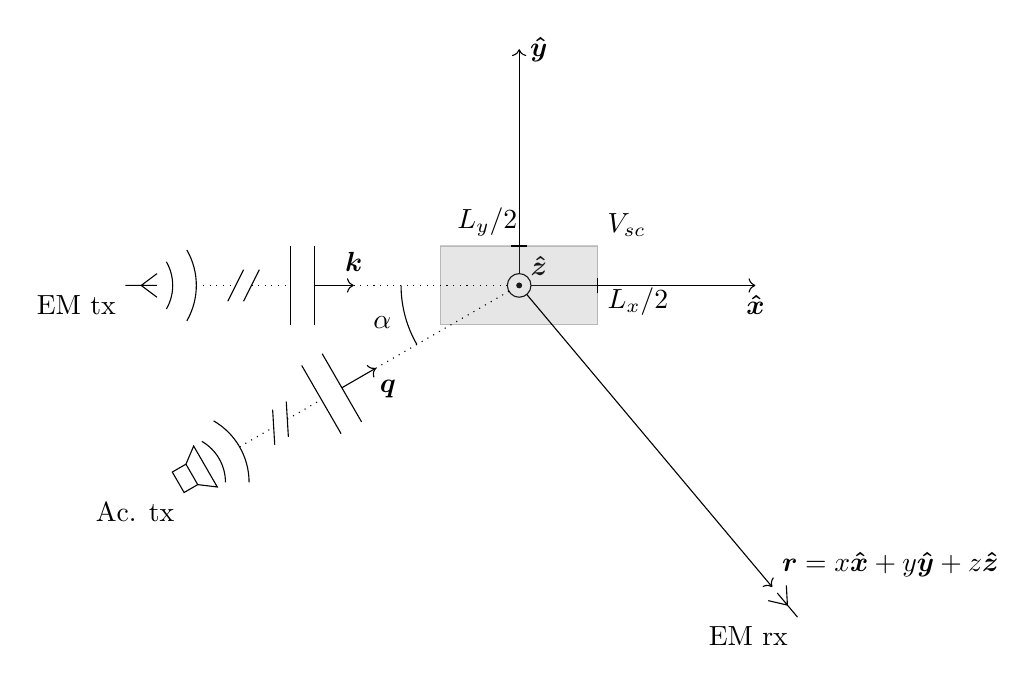
\begin{tikzpicture}
			% Draw coordinate axes
			\draw (0,0) circle(0.15);
			\filldraw[black] circle(0.03);
			\draw[->] (0.15,0) -- (3,0);
			\draw[->] (0,.150) -- (0,3);
			\draw (3,-0.25) node{$\bm{\hat{x}}$} (0.25,3) node{$\bm{\hat{y}}$} (0.25,0.25) node{$\bm{\hat{z}}$};
			
			% Draw scattering cube (or rectangle in this case)
			\draw[fill=gray,opacity=0.2] (-1,-0.5) rectangle(1,0.5);
			\draw (1,-0.1) -- (1,0.1) node[anchor= north west]{$L_{x}/2$} (-0.1,0.5) -- (0.1,0.5) node[anchor= south east]{$L_{y}/2$} (1,0.5) node[anchor=south west]{$V_\mrm{sc}$};
			
			% Draw EM tx and spherical waves
			\draw[shift = {(-5,0)}] (0,0) node[anchor=north east]{EM tx} -- (0.4,0) (0.2,0) -- (0.4,0.15)
			(0.2,0) -- (0.4,-0.15);
			\draw[shift = {(-5,0)}] ([shift={(-30:0.6)}] 0,0) arc(-30:30:0.6) ([shift={(-30:0.9)}] 0,0) arc(-30:30:0.9);
			
			% Draw EM "long distance" lines
			\draw[shift = {(-4.1,0)},dotted] (0,0) -- (0.5,0) (0.7,0) -- (1.2,0);
			\draw[shift = {(-4.1,0)}] (0.4,-0.2) -- (0.6,0.2) (0.6,-0.2) -- (0.8,0.2);
			
			% Draw EM plane waves
			\draw[shift = {(-2.9,0)}] (0,-0.5) -- (0,0.5) (0.3,-0.5) -- (0.3,0.5);
			\draw[shift = {(-2.6,0)}, ->] (0,0) -- (0.5,0);
			\draw[shift = {(-2.6,0)}] (0.5,0.3) node{$\bm{k}$};
			\draw[dotted] (-0.15,0) -- (-2.1,0);
			
			% Draw Ac. tx and spherical waves
			\draw[shift = {(210:5)}, rotate = 30] (0,-0.15) node[anchor=north east]{Ac. tx} rectangle (0.2,0.15) -- (0.4,0.3) -- (0.4,-0.3) -- (0.2,-0.15);
			\draw[shift = {(210:5)}, rotate = 30] ([shift={(-30:0.6)}] 0,0) arc(-30:30:0.6) ([shift={(-30:0.9)}] 0,0) arc(-30:30:0.9);
			
			% Draw Ac. "long distance" lines
			\draw[shift = {(210:4.1)}, rotate = 30,dotted] (0,0) -- (0.5,0) (0.7,0) -- (1.2,0);
			\draw[shift = {(210:4.1)}, rotate = 30] (0.4,-0.2) -- (0.6,0.2) (0.6,-0.2) -- (0.8,0.2);
			
			% Draw Ac. plane waves
			\draw[shift = {(210:2.9)}, rotate = 30] (0,-0.5) -- (0,0.5) (0.3,-0.5) -- (0.3,0.5);
			\draw[shift = {(210:2.6)}, rotate = 30, ->] (0,0) -- (0.5,0);
			\draw[shift = {(210:2.6)}, rotate = 30] (0.5,-0.3) node{$\bm{q}$};
			\draw[rotate = 30, dotted] (-0.15,0) -- (-2.1,0);
			
			% Draw angle alpha
			\draw ([shift={(180:1.5)}] 0,0) arc(180:210:1.5) (195:1.8) node{$\alpha$};
			
			% Draw line towards receiver
			\draw[->] (310:0.15) -- (310:5) node[anchor=south west]{$\bm{r} = x\bm{\hat{x}} + y\bm{\hat{y}} + z\bm{\hat{z}}$};
			
			% Draw EM rx
			\draw[shift = {(310:5.5)}, rotate = 130] (0,0) node[anchor=north east]{EM rx} -- (0.4,0) (0.2,0) -- (0.4,0.15) (0.2,0) -- (0.4,-0.15);
		\end{tikzpicture}
		}
		\caption{\label{fig:app-radar-geom} Geometry for the scattering problem.}
	\end{figure}
	The $xy$-plane is defined as the plane formed by the acoustic and electromagnetic wavevectors (they are assumed to be non-parallel). The scattering volume is centered in the origin of the coordinate system, and both the acoustic and electromagnetic waves are approximated as plane waves close to the origin. Thus, the electromagnetic and dielectric perturbation fields near the origin are defined as
	\begin{align}
		\bm{E}_\mrm{i} (\bm{r}',t) &= \bm{E}_\mrm{i} (\bm{r}') = \bm{E}_{\mrm{i}0} \eu^{\iu \bm{k}\cdot\bm{r}'} \label{eq:app-radar-planeE} \\
		\varepsilon_1 (\bm{r}',t) &= \frac{\varepsilon_\mrm{r}^2 \mathfrak{p}}{K} p_0 \cos(\bm{q} \cdot \bm{r}' - \Omega t) \label{eq:app-radar-planeEps}
	\end{align}
	Here, $\bm{E}_{\mrm{i}0}$ is the complex field amplitude at the origin ($-\iu\omega t$ time-dependence separated) and $\bm{k}$ is the electromagnetic wavevector. The scalar photoelastic relation from equation \eqref{eq:th-PE-scalar-p} has been used, where $\mathfrak{p}$ is the photoelastic constant, $p_0$ is the acoustic pressure amplitude at the origin, $K$ is the bulk modulus, $\bm{q}$ is the acoustic wavevector and $\Omega$ the acoustic frequency.
	
	For simplicity, the electromagnetic polarization is assumed to be in z, $\bm{E}_{\mrm{i}0} \parallel \bm{\hat{z}}$. This is also in part done to avoid polarization changes in the scattered field \cite{Korpel1988}. Due to this $\nabla(\bm{E}_\mrm{i} \cdot \nabla \varepsilon_1) = \bm{0}$ which simplifies the scattering integral to
	\begin{equation*}
		\bm{E}_\mrm{sc}(\bm{r},t) = \frac{k^2}{4\pi\varepsilon_\mrm{r}} \int_{V_\mrm{sc}} \frac{\eu^{\iu k |\bm{r}-\bm{r'}| }}{ |\bm{r}-\bm{r'}|} \bm{E}_\mrm{i} (\bm{r'},t) \varepsilon_1 (\bm{r'},t) \mathrm{d}v'
	\end{equation*}
	Insertion of equation \eqref{eq:app-radar-planeE} and \eqref{eq:app-radar-planeEps} gives
	\begin{equation*}
		\bm{E}_\mrm{sc}(\bm{r},t) = \frac{k^2}{4\pi\varepsilon_\mrm{r}} \int_{V_\mrm{sc}} \frac{\eu^{\iu k |\bm{r}-\bm{r'}| }}{ |\bm{r}-\bm{r'}|} \bm{E}_{\mrm{i}0} \eu^{\iu \bm{k} \cdot \bm{r}'} \frac{\varepsilon_\mrm{r}^2 \mathfrak{p}}{K} p_0 \cos(\bm{q} \cdot \bm{r}' - \Omega t) \mathrm{d}v'
	\end{equation*}
	Assuming far-field gives an approximation for the Green-function as \cite{Kristensson2008}
	\begin{equation*}
		\frac{\eu^{\iu k |\bm{r}-\bm{r'}| }}{ |\bm{r}-\bm{r'}|} \approx \frac{\eu^{\iu kr}}{r} \eu^{-\iu k \bm{\hat{r}} \cdot \bm{r}'}
	\end{equation*}
	where $r = |\bm{r}|$ and $\bm{\hat{r}} = \bm{r}/r$. The scattering integral is now written as
	\begin{equation*}
		\bm{E}_\mrm{sc}(\bm{r},t) = \frac{\varepsilon_\mrm{r}k^2 \eu^{\iu kr} \bm{E}_{\mrm{i}0} \mathfrak{p} p_0}{4\pi r K} \int_{V_\mrm{sc}} \eu^{\iu k ( \bm{\hat{k}} - \bm{\hat{r}} ) \cdot \bm{r}'} \cos(\bm{q} \cdot \bm{r}' - \Omega t) \mathrm{d}v'
	\end{equation*}
	The cosine is now written as complex exponentials giving
	\begin{equation*}
	\begin{split}
			\bm{E}_\mrm{sc}(\bm{r},t) =& \frac{\varepsilon_\mrm{r}k^2 \eu^{\iu kr} \bm{E}_{\mrm{i}0} \mathfrak{p} p_0}{8\pi r K} \\
			&\cdot \left( \eu^{-\iu \Omega t} \int_{V_\mrm{sc}} \eu^{\iu ( k(\bm{\hat{k}} - \bm{\hat{r}}) + \bm{q} ) \cdot \bm{r}'} \mathrm{d}v + \eu^{\iu \Omega t} \int_{V_\mrm{sc}} \eu^{\iu ( k(\bm{\hat{k}} - \bm{\hat{r}}) - \bm{q} ) \cdot \bm{r}'} \mathrm{d}v' \right)
	\end{split}
	\end{equation*}
	The two integrals are of the same form, $\int \eu^{\iu \bm{A} \cdot \bm{r}'} \mathrm{d}v'$, where $\bm{A}$ is independent of $\bm{r}'$. This is solved in general below for the cuboid volume defined by $-L_m/2 \leq m \leq L_m/2$, $m = x,y,z$.
	\begin{equation*}
	\begin{split}
		\int_{V_\mrm{sc}} \eu^{\iu \bm{A} \cdot \bm{r}'} \mathrm{d}v' &=
		\int_{V_\mrm{sc}} \eu^{\iu \bm{A} \cdot \bm{\hat{x}} x'} \eu^{\iu \bm{A} \cdot \bm{\hat{y}} y'} \eu^{\iu \bm{A} \cdot \bm{\hat{z}} z'} \mathrm{d}v' \\
		&= \prod_{m = x,y,z} \frac{1}{\iu \bm{A} \cdot \bm{\hat{m}}} \left( \eu^{\iu \bm{A} \cdot \bm{\hat{m}} L_m/2} - \eu^{-\iu \bm{A} \cdot \bm{\hat{m}} L_m/2} \right) \\
		&= \prod_{m = x,y,z} \frac{2}{\bm{A} \cdot \bm{\hat{m}}} \sin \left(\bm{A} \cdot \bm{\hat{m}} \frac{L_m}{2} \right) 
		= \prod_{m = x,y,z} L_m \text{sinc} \left( \frac{\bm{A} \cdot \bm{\hat{m}} L_m}{2\pi} \right)
	\end{split}
	\end{equation*}
	where sinc$(x) = \sin(\pi x)/(\pi x)$. To apply this result to $\bm{A} = k(\bm{\hat{k}} - \bm{\hat{r}}) \pm \bm{q}$ this is first simplified using the geometry defined earlier.
	\begin{equation*}
		k(\bm{\hat{k}} - \bm{\hat{r}}) \pm \bm{q} = k\bm{\hat{x}} - k(\bm{\hat{x}} x + \bm{\hat{y}} y + \bm{\hat{z}} z)/r \pm q(\bm{\hat{x}} \cos{\alpha} + \bm{\hat{y}} \sin{\alpha})
	\end{equation*}
	where r is not written out fully. $\bm{A} \cdot \bm{\hat{m}}$ are now calculated for the three coordinate axes as
	\begin{equation} 
	\begin{split}
		\bm{A} \cdot \bm{\hat{x}} &= k - kx/r \pm q\cos{\alpha} = k - k\sin{\theta}\cos{\phi} \pm q\cos{\alpha} \\
		\bm{A} \cdot \bm{\hat{y}} &= - ky/r \pm q\sin{\alpha} = - k\sin{\theta}\sin{\phi} \pm q\sin{\alpha} \\
		\bm{A} \cdot \bm{\hat{z}} &= -kz/r = -k\cos{\theta}
	\end{split}
	\label{eq:radar-Aproj}
	\end{equation}
	where a conversion to spherical coordinates was made. Insertion into the integral solution gives:
	\begin{equation}
		\begin{split} 
			\int_{V_\mrm{sc}} &\eu^{\iu (	k(\bm{\hat{k}} - \bm{\hat{r}}) \pm \bm{q}) \cdot \bm{r}'} \mathrm{d}v' \\
			=& L_{x} \text{sinc} \left( \frac{L_{x}}{2\pi} ( k - k\sin{\theta}\cos{\phi} \pm q\cos{\alpha} ) \right) \\
			&\cdot L_{y} \text{sinc} \left( \frac{L_{y}}{2\pi} ( - k\sin{\theta}\sin{\phi} \pm q\sin{\alpha} ) \right)
			\cdot L_{z} \text{sinc} \left( -\frac{L_{z}}{2\pi} k\cos{\theta} \right) \\
			=& L_{x} L_{y} L_{z} \Phi^\pm (\theta,\phi)
		\end{split}
		\label{eq:radar-intsol}
	\end{equation}
	where all angular dependence has been gathered in the function $\Phi^\pm (\theta,\phi)$. This result is now inserted into the scattered field, giving
	\begin{equation*}
	\begin{split}
		\bm{E}_\mrm{sc}(\bm{r},t) &= \frac{\varepsilon_\mrm{r}k^2 \eu^{\iu kr} \bm{E}_{\mrm{i}0} \mathfrak{p} p_0}{8\pi r K} L_{x} L_{y} L_{z} \left( \eu^{-\iu \Omega t} \Phi^+ (\theta,\phi)  + \eu^{\iu \Omega t} \Phi^- (\theta,\phi) \right) \\
		&= \bm{E}_{\mrm{i}0} E_\mrm{A}(\bm{r},t)
	\end{split}
	\end{equation*}
	
	By inspecting $E_\mrm{A}(\bm{r},t)$ it is clear that two frequency-shifted components arise. Since the implied time-dependence is $\eu^{-\iu \omega t}$, the factors $e^{\mp \iu \Omega t}$ give a frequency shift of $\pm \Omega$. The scattered field is written using two distinct components as
	\begin{equation*}
	\bm{E}_\mrm{sc} (\bm{r},t) = \bm{E}_\mrm{sc}^+ (\bm{r},t) + \bm{E}_\mrm{sc}^- (\bm{r},t) = \bm{E}_{\mrm{i}0} \left( E_\mrm{A}^+ (\bm{r},t) + E_\mrm{A}^- (\bm{r},t) \right)
	\end{equation*}
	where
	\begin{equation*}
		E_\mrm{A}^\pm (\bm{r},t) = \frac{\varepsilon_\mrm{r}k^2 \eu^{\iu kr} \mathfrak{p} p_0}{8\pi r K} L_{x} L_{y} L_{z} e^{\mp \iu \Omega t} \Phi^\pm (\theta,\phi)
	\end{equation*}
	
	\subsection{Solution in terms of power \label{sec:app-derivations-radar-power}}
	This treatment has primarily been focused around the electric field. To obtain a more practical expression, this is now transformed into power. The power is calculated for the individual frequency shifted components, since they are distinct and single-frequency. The time average for one frequency component of the Poynting vector is \cite{Kristensson2008}
	\begin{equation*}
	\begin{split}
		\left< \bm{S}_\mrm{sc}^\pm \right> (\bm{r}) &= \frac{1}{2} \mathrm{Re}\left\{ \left( \bm{E}_\mrm{sc}^\pm (\bm{r}, t) \eu^{-i\omega t} \right) \times \left( \bm{H}_\mrm{sc}^{\pm} (\bm{r}, t) \eu^{-i\omega t} \right)^* \right\} \\
		&= \frac{1}{2} \mathrm{Re}\left\{ \bm{E}_\mrm{sc}^\pm (\bm{r}, t) \times \bm{H}_\mrm{sc}^{\pm} (\bm{r}, t)^* \right\}
	\end{split}
	\end{equation*}
	where the time-dependence of the incident electromagnetic wave was re-introduced. The magnetic field $\bm{H}_\mrm{sc}^\pm (\bm{r}, t)$ is given by \cite{Kristensson2008}
	\begin{equation*}
		\bm{H}_\mrm{sc}^\pm (\bm{r}, t) \approx \frac{1}{\iu k \eta_0 \eta} \nabla \times \bm{E}_\mrm{sc}^\pm (\bm{r}, t)
	\end{equation*}
	where $\eta_0$ is the wave impedance of free space and $\eta_0 \eta$ the wave impedance in the material. An approximation has been made for $k$, where this is assumed to have the same value as before scattering. Since there is a frequency shift this is known to not be the case, but given a small acoustic frequency compared to the electromagnetic frequency, the error is small. The curl of $\bm{E}_\mrm{sc}^\pm (\bm{r}, t)$ is now written as
	\begin{equation*}
		\nabla \times \bm{E}_\mrm{sc}^\pm (\bm{r}, t) = \nabla \times (\bm{E}_{\mrm{i}0} E_\mrm{A}^\pm (\bm{r},t)) = \nabla E_\mrm{A}^\pm (\bm{r},t) \times \bm{E}_{\mrm{i}0}
	\end{equation*}
	In spherical coordinates the gradient is written \addref
	\begin{equation*}
		\nabla f = \frac{\partial f}{\partial r} \bm{\hat{r}} + \frac{1}{r} \frac{\partial f}{\partial \theta} \bm{\hat{\theta}} + \frac{1}{r\sin{\theta}} \frac{\partial f}{\partial \phi} \bm{\hat{\phi}}
	\end{equation*}
	$E_\mrm{A}^\pm (\bm{r}, t)$ contains a factor $1/r$, so the two last terms in the gradient will be $\sim 1/r^2$ and are neglected. The gradient is now written as
	\begin{equation*}
	\begin{split}
		\nabla E_\mrm{A}^\pm (\bm{r}, t) &\approx \frac{\partial E_\mrm{A}}{\partial r} \bm{\hat{r}} \\
		&= \left( \frac{\iu k\eu^{\iu kr}}{r} - \frac{\eu^{\iu kr}}{r^2} \right) \frac{\varepsilon_\mrm{r}k^2 \mathfrak{p} p_0}{8\pi K} L_{x} L_{y} L_{z} \left( \eu^{- \iu \Omega t} \Phi^+ (\theta,\phi) + \eu^{\iu \Omega t} \Phi^- (\theta,\phi) \right) \bm{\hat{r}} \\
		&\approx \iu kE_\mrm{A}^\pm (\bm{r}, t) \bm{\hat{r}}
	\end{split}
	\end{equation*}
	where the $1/r^2$ term was neglected. These results are inserted into the expression for the magnetic field, giving
	\begin{equation*}
		\bm{H}_\mrm{sc}^\pm (\bm{r}, t) = \frac{1}{\iu k \eta_0 \eta} (\iu kE_\mrm{A}^\pm (\bm{r}, t) \bm{\hat{r}} \times \bm{E}_{\mrm{i}0}) = \frac{E_\mrm{A}^\pm (\bm{r}, t)}{ \eta_0 \eta} \bm{\hat{r}} \times \bm{E}_{\mrm{i}0}
	\end{equation*}
	Now, the cross product with the electric field is calculated as
	\begin{equation*}
	\begin{split}
		\bm{E}_\mrm{sc}^\pm (\bm{r}, t) \times \bm{H}_\mrm{sc}^{\pm} (\bm{r}, t)^* &= E_\mrm{A}^\pm (\bm{r}, t) \bm{E}_{\mrm{i}0} \times \left( \frac{E_\mrm{A}^\pm (\bm{r}, t)}{ \eta_0 \eta} \bm{\hat{r}} \times \bm{E}_{\mrm{i}0} \right)^* \\
		&= \frac{|E_\mrm{A}^\pm (\bm{r}, t)|^2}{\eta_0 \eta} \left( \bm{\hat{r}} (\bm{E}_{\mrm{i}0} \cdot \bm{E}_{\mrm{i}0}^*) - \bm{E}_{\mrm{i}0}^* (\bm{E}_{\mrm{i}0} \cdot \bm{\hat{r}}) \right)
	\end{split}
	\end{equation*}
	In the far-field $\bm{E}_\mrm{sc} \cdot \bm{\hat{r}} = 0$ \addref and since $\bm{E}_\mrm{sc} \parallel \bm{E}_{\mrm{i}0}$ the cross product is simplified to
	\begin{equation*}
		\bm{E}_\mrm{sc}^\pm (\bm{r}, t) \times \bm{H}_\mrm{sc}^{\pm} (\bm{r}, t)^* = \frac{\bm{\hat{r}}}{\eta_0 \eta} |\bm{E}_{\mrm{i}0}|^2 |E_\mrm{A}^\pm (\bm{r},t)|^2
	\end{equation*}
	The time-averaged Poynting vector is now calculated as
	\begin{equation*}
		\left< \bm{S}_\mrm{sc}^\pm \right> (\bm{r}) = \frac{1}{2}\mathrm{Re}\left\{ \bm{E}_\mrm{sc}^\pm (\bm{r}, t) \times \bm{H}_\mrm{sc}^{\pm} (\bm{r}, t)^* \right\} = \frac{\bm{\hat{r}}}{2\eta_0 \eta} |\bm{E}_{\mrm{i}0}|^2 |E_\mrm{A}^\pm (\bm{r},t)|^2
	\end{equation*}
	where $|E_\mrm{A}^\pm (\bm{r},t)|^2$ is given by
	\begin{equation*}
		|E_\mrm{A}^\pm (\bm{r},t)|^2 = \frac{\varepsilon_\mrm{r}^2 k^4 \mathfrak{p}^2 p_0^2}{64\pi^2 r^2 K^2} L_{x}^2 L_{y}^2 L_{z}^2 \Phi^\pm (\theta,\phi)^2
	\end{equation*}
	
	To find an expression for $|\bm{E}_{\mrm{i}0}|^2$, the field from the transmitter antenna is written as (adapted from \cite{Orfanidis2016})
	\begin{equation*}
		\bm{E}_\mrm{T} (\bm{r}) = \iu k\eta_0\eta \frac{\eu^{\iu kr}}{4\pi r} \bm{F}_\perp (\bm{\hat{r}})
	\end{equation*}
	where $\bm{F}_\perp$ is the far-field amplitude. Now the coordinate system is not the same as earlier in the derivation! Here it is a spherical coordinate system with origin at the transmitting antenna. This corresponds to a translation in $-\bm{\hat{x}}$ of the original coordinate system. Let $R_\mrm{T}$ be the distance between the two coordinate systems, or equivalently the distance from the transmitter to the scattering center. The direction to the scattering center in this new system is denoted $\bm{\hat{r}}_{sc} = \bm{r}_{sc}/R_\mrm{T}$. Assuming that the orientations of the transmitter and scattering coordinate systems are the same, $|\bm{E}_{\mrm{i}0}|^2$ can be written in the transmitter system as \cite{Orfanidis2016}
	\begin{equation*}
		|\bm{E}_{\mrm{i}0}|^2 = |\bm{E}_\mrm{T}(\bm{r}_{sc})|^2 = \left| \iu k\eta_0\eta \frac{\eu^{\iu kR_\mrm{T}}}{4\pi R_\mrm{T}} \bm{F}_\perp (\bm{\hat{r}}_{sc}) \right|^2 = \frac{k^2 \eta_0^2 \eta^2}{16 \pi^2 R_\mrm{T}^2} |\bm{F}_\perp (\bm{\hat{r}}_{sc})|^2 = 2\eta_0 \eta \mathcal{P}(\bm{\hat{r}}_{sc})
	\end{equation*}
	If the maximum gain $G_\mrm{T}$ of the antenna is in the direction $\hat{r}_{sc}$, it holds that \cite{Orfanidis2016}
	\begin{equation*}
		\mathcal{P}(\bm{\hat{r}}_{sc}) = \frac{P_\mrm{T} G_\mrm{T}}{4\pi R_\mrm{T}^2}
	\end{equation*}
	where $P_\mrm{T}$ is the power accepted by the antenna. This is used to write
	\begin{equation*}
		|\bm{E}_{\mrm{i}0}|^2 = 2\eta_0 \eta \frac{P_\mrm{T} G_\mrm{T}}{4\pi R_\mrm{T}^2}
	\end{equation*}
	Now this is inserted into the time-average of the power density
	\begin{equation*}
		\left< \bm{S}_\mrm{sc}^\pm \right> (\bm{r}) = \bm{\hat{r}} \frac{P_\mrm{T} G_\mrm{T}}{4\pi R_\mrm{T}^2} \frac{\varepsilon_\mrm{r}^2 k^4 \mathfrak{p}^2 p_0^2}{64\pi^2 r^2 K^2} L_{x}^2 L_{y}^2 L_{z}^2 \Phi^\pm (\theta,\phi)^2
	\end{equation*}
	
	Now the effects of the receiving antenna are considered. It is assumed that this antenna is optimally directed towards the scattering center. The received power is then
	\begin{equation*}
		P_\mrm{R}^\pm = \left| \left< \bm{S}_\mrm{sc}^\pm \right> (R_\mrm{R}, \theta, \phi) \right| A_\mrm{e}
	\end{equation*}
	where $R_\mrm{R}$ is the distance between the scattering center and the receiver, and the receiver is located in the direction $(\theta,\phi)$ as seen from the scattering center. $A_\mrm{e}$ is the effective area of the antenna, which can be rewritten as
	\begin{equation*}
		A_\mrm{e} = \frac{\lambda_\mrm{R}^2 G_\mrm{R}}{4\pi}
	\end{equation*}
	where $G_\mrm{R}$ is the gain of the receiving antenna. $\lambda_\mrm{R}$ should be the wavelength at the antenna here, which is not necessarily the same as in the material. Combining this with earlier results gives a received power of
	\begin{equation*}
		P_\mrm{R}^\pm = \frac{\lambda_\mrm{R}^2 G_\mrm{R}}{4\pi} \frac{P_\mrm{T} G_\mrm{T}}{4\pi R_\mrm{T}^2} \frac{\varepsilon_\mrm{r}^2 k^4 \mathfrak{p}^2 p_0^2}{64\pi^2 R_\mrm{R}^2 K^2} L_{x}^2 L_{y}^2 L_{z}^2 \Phi^\pm (\theta,\phi)^2
	\end{equation*}
	For a more traditional bistatic radar equation \cite{Richards2012} this can be written as
	\begin{equation*}
		P_\mrm{R}^\pm = \frac{P_\mrm{T} G_\mrm{T} G_\mrm{R} \lambda_\mrm{R}^2 \sigma^\pm (\theta,\phi)}{(4\pi)^3 R_\mrm{T}^2 R_\mrm{R}^2}
	\end{equation*}
	with the radar cross-section given by
	\begin{equation*}
		\sigma^\pm (\theta, \phi) = \frac{\varepsilon_\mrm{r}^2 k^4 \mathfrak{p}^2 p_0^2}{16\pi K^2} L_{x}^2 L_{y}^2 L_{z}^2 \Phi^\pm (\theta,\phi)^2
	\end{equation*}
	
	\subsection{Signal-to-noise ratio and coherent integration \label{sec:app-derivations-radar-SNR}}
	A more practical measurement than received power is signal-to-noise ratio (SNR). For this, the average noise power is described as \cite{Young2004}
	\begin{equation*}
		P_\mrm{n} = k_\mrm{B} TB
	\end{equation*}
	where $k_\mrm{B}$ is Boltzmann's constant, $T$ is the temperature and $B$ is the utilized receiver bandwidth. The noise power picked up by the antenna is calculated using the standard temperature $T_0 = 290$ K. The SNR directly at the antenna can thus be written as
	\begin{equation*}
		\mathit{SNR}^\pm_\mrm{ant} \frac{P_\mrm{T} G_\mrm{T} G_\mrm{R} \lambda_\mrm{R}^2 \sigma^\pm (\theta,\phi)}{(4\pi)^3 R_\mrm{T}^2 R_\mrm{R}^2 k_\mrm{B} T_0 B}
	\end{equation*}
	After the antenna is the RF front-end which usually contains a bandpass filter, low-noise amplifier (LNA), and mixer. Here the received signal is amplified so that it can be further processed. The amplification affects both the signal and noise, but the electronic components add more noise which causes the SNR to deteriorate. To quantify this, the concept of noise ratio and noise figure is used. The noise ratio is defined as \cite{Young2004}
	\begin{equation*}
		F = \frac{\mathit{SNR}_\mrm{i}}{\mathit{SNR}_\mrm{o}}
	\end{equation*}
	where the SNR's are in linear units, i denotes input and o denotes output. It is more common to use noise figure, which is simply the noise ratio expressed in dB units, $\mathit{NF} = 10\log_{10}(F)$. After the RF front-end the signal is often strong enough to not be affected by further noise, so it is usually sufficient to use a noise ratio/figure for that part of the receiver. The SNR after the receiver can now be written using the noise ratio as
	\begin{equation*}
		\mathit{SNR}^\pm = \frac{P_\mrm{T} G_\mrm{T} G_\mrm{R} \lambda_\mrm{R}^2 \sigma^\pm (\theta,\phi)}{(4\pi)^3 R_\mrm{T}^2 R_\mrm{R}^2 k_\mrm{B} T_0 B \cdot F}
	\end{equation*}
	One more effect is added to this, and that is signal integration in the signal processing following the receiver. Noise can often be modeled as a random process, and if multiple samples are added together the noise can be averaged out. If coherent demodulation is used, $N$ samples added together will cause the SNR to improve by a factor $N$ \cite{Richards2012}. The SNR can then be written as
	\begin{equation*}
		\mathit{SNR}^\pm_N = \frac{P_\mrm{T} G_\mrm{T} G_\mrm{R} \lambda_\mrm{R}^2 \sigma^\pm (\theta,\phi)}{(4\pi)^3 R_\mrm{T}^2 R_\mrm{R}^2 k_\mrm{B} T_0 B F} N
	\end{equation*}
	
	\section{Refined interaction region} \label{sec:app-derivations-refined}
	The derivation in \ref{sec:app-derivations-radar} is based on plane waves and a very simple geometry. A problem with the geometry used is that there is no easy way to obtain the parameters $L_{x}$, $L_{y}$ and $L_{z}$ from common parameters of the acoustic and electromagnetic beams. To address this, a slightly different interaction geometry based on beams is introduced as shown in figure \ref{fig:parallelogram}. Here the beam diameters $d_\mrm{e}$ and $d_\mrm{a}$ have been introduced for the electromagnetic and acoustic plane waves. For simplicity, it is assumed that the beam edges are infinitely sharp, i.e. inside the wave behaves as a plane wave and outside it is zero. This way the previous derivation can be used with the exception of the interaction region.
	\begin{figure}[h]
		\centering
		\resizebox{\textwidth}{!}{
			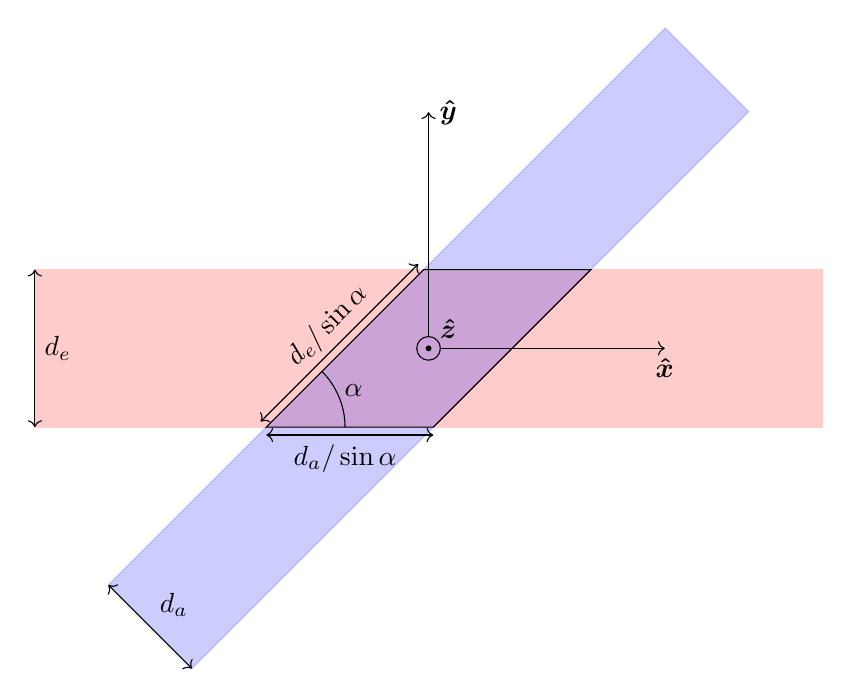
\begin{tikzpicture}
	
	
	% Draw EM beam
	\filldraw[red,opacity=0.2] (-5,-1) rectangle(5,1);
	\draw[<->] (-5,-1) -- (-5,1);
	\draw (-5,0) node[anchor=west]{$d_e$};
	
	% Draw Ac beam
	\filldraw[blue,rotate=45,opacity=0.2] (-5,-0.75) rectangle(5,0.75);
	\draw[<->,rotate=45] (-5,-0.75) -- (-5,0.75);
	\draw[rotate=45] (-5,0) node[anchor=south west]{$d_a$};
	
	% Draw parallelogram
	\draw (-2.061,-1) -- (-0.061,1) -- (2.061,1) -- (0.061,-1) -- cycle;
	\draw[<->] (-2.061,-1.1) -- (0.061, -1.1);
	\draw (-1.061, -1.4) node{$d_a/\sin{\alpha}$};
	\draw[<->, shift={(135:0.1)}] (-2.061,-1) -- (-0.061,1);
	\draw[shift={(135:0.4)}] (-1,0) node[anchor=center,rotate=45] {$d_e/\sin{\alpha}$};
	
	% Draw angle alpha
	\draw ([shift={(-1.061,-1)}] 0,0) arc(0:45:1) ([shift={(22.5:1.2)}] -2.061,-1) node{$\alpha$};
	
	% Draw coordinate axes
	\draw (0,0) circle(0.15);
	\filldraw[black] circle(0.03);
	\draw[->] (0.15,0) -- (3,0);
	\draw[->] (0,.150) -- (0,3);
	\draw (3,-0.25) node{$\bm{\hat{x}}$} (0.25,3) node{$\bm{\hat{y}}$} (0.25,0.25) node{$\bm{\hat{z}}$};
	
\end{tikzpicture}
		}
		\caption{\label{fig:parallelogram} Parallelogram interaction region}
	\end{figure}
	Since plane waves are still used the model is not based on real beams. However, for real beams it is still easy to obtain widths at the overlap area and then the interaction region should be fairly close using this model.
	
	The integration limits corresponding to this parallelogram can be written as
	\begin{align*}
		x_0 - x_1 &< x < x_0 + x_1 \\
		-d_\mrm{e}/2 &< y < d_\mrm{e}/2 \\
		-L_{z}/2 &< z < L_{z}/2
	\end{align*}
	where
	\begin{align*}
		x_0 &= \frac{y}{\tan{\alpha}} \\
		x_1 &= \frac{d_\mrm{a}}{2\sin{\alpha}}
	\end{align*}
	The solution to the integral for a general function on the form $\eu^{\iu \bm{A} \cdot \bm{r}}$ is now written as
	\begin{equation*}
	\begin{split}
			I &= \int_{V_\mrm{sc}} \eu^{\iu \bm{A} \cdot \bm{r}'} \mathrm{d}v' \\
			&= \int_{-L_{z}/2}^{L_{z}/2} \eu^{\iu \bm{A} \cdot \bm{\hat{z}} z'} \mathrm{d}z'
			\int_{-d_\mrm{e}/2}^{d_\mrm{e}/2} \left( \eu^{\iu \bm{A} \cdot \bm{\hat{y}} y'}
			\int_{x_0-x_1}^{x_0+x_1} \eu^{\iu \bm{A} \cdot \bm{\hat{x}} x'} \mathrm{d}x' \right) \mathrm{d}y' \\
			&= \int_{-L_{z}/2}^{L_{z}/2} \eu^{\iu \bm{A} \cdot \bm{\hat{z}} z'} \mathrm{d}z' \cdot I_2
	\end{split}
	\end{equation*}
	using the solution from \ref{sec:app-derivations-radar} \todoint{Maybe make better references?} this integral can be written as
	\begin{equation*}
		I = L_{z} \text{sinc}\left( \frac{\bm{A} \cdot \bm{\hat{z}} L_{z}}{2\pi} \right) \cdot I_2
	\end{equation*}
	The integral $I_2$ can be solved as
	\begin{equation*}
	\begin{split}
		I_2 &= \int_{-d_\mrm{e}/2}^{d_\mrm{e}/2} \eu^{\iu \bm{A} \cdot \bm{\hat{y}} y'}
		\cdot \frac{1}{\iu \bm{A} \cdot \bm{\hat{x}}}
		\left( \eu^{\iu \bm{A} \cdot \bm{\hat{x}} (x_0+x_1)} - \eu^{\iu \bm{A} \cdot \bm{\hat{x}} (x_0-x_1)}\right) \mathrm{d}y' \\
		&=\int_{-d_\mrm{e}/2}^{d_\mrm{e}/2} \eu^{\iu \bm{A} \cdot \bm{\hat{y}} y'}
		\cdot \eu^{\iu \bm{A} \cdot \bm{\hat{x}} x_0} \frac{2}{\bm{A} \cdot \bm{\hat{x}}} \sin(\bm{A} \cdot \bm{\hat{x}} x_1) \mathrm{d}y' \\
		&=\int_{-d_\mrm{e}/2}^{d_\mrm{e}/2} \eu^{\iu \bm{A} \cdot (\bm{\hat{y}} y'+ \bm{\hat{x}} x_0)}
		\cdot 2x_1 \text{sinc}\left( \frac{\bm{A} \cdot \bm{\hat{x}} x_1}{\pi} \right) \mathrm{d}y' \\
		&= \frac{d_\mrm{a}}{\sin{\alpha}} \text{sinc}\left( \frac{\bm{A} \cdot \bm{\hat{x}} d_\mrm{a}}{2\pi \sin{\alpha}} \right) \int_{-d_\mrm{e}/2}^{d_\mrm{e}/2} \eu^{\iu \bm{A} \cdot (\bm{\hat{y}} + \bm{\hat{x}}/\tan{\alpha}) y'} \mathrm{d}y' \\
		&= \frac{d_\mrm{a}}{\sin{\alpha}} \text{sinc}\left( \frac{\bm{A} \cdot \bm{\hat{x}} d_\mrm{a}}{2\pi \sin{\alpha}} \right) \cdot I_3
	\end{split}
	\end{equation*}
	The integral $I_3$ can be solved analogously to the solution from \ref{sec:app-derivations-radar} as
	\begin{equation*}
		I_3 = d_\mrm{e} \text{sinc}\left( \frac{\bm{A} \cdot (\bm{\hat{y}} + \bm{\hat{x}}/\tan{\alpha}) d_\mrm{e}}{2\pi} \right)
	\end{equation*}
	Now the complete solution to $I$ is written as
	\begin{equation*}
	\begin{split}
		I =& \frac{d_\mrm{a}}{\sin{\alpha}} \text{sinc}\left( \frac{\bm{A} \cdot \bm{\hat{x}} d_\mrm{a}}{2\pi \sin{\alpha}} \right) \cdot d_\mrm{e} \text{sinc}\left( \frac{\bm{A} \cdot (\bm{\hat{y}} + \bm{\hat{x}}/\tan{\alpha}) d_\mrm{e}}{2\pi} \right) \\
		&\cdot L_{z} \text{sinc}\left( \frac{\bm{A} \cdot \bm{\hat{z}} L_{z}}{2\pi} \right)
	\end{split}
	\end{equation*}
	If the specific function of interest to the scattering problem is inserted, and spherical coordinates are used as in equation \eqref{eq:radar-Aproj} the solution is
	\begin{equation*}
	\begin{split}
		\int_{V_\mrm{sc}} &\eu^{\iu (	k(\bm{\hat{k}} - \bm{\hat{r}}) \pm \bm{q}) \cdot \bm{r}'} \mathrm{d}v' \\
		&= \frac{d_\mrm{a} d_\mrm{e} L_{z}}{\sin{\alpha}} \text{sinc}\left( \frac{d_\mrm{a}}{2\pi \sin{\alpha}}(k - k\sin{\theta}\cos{\phi} \pm q\cos{\alpha}) \right) \\
		&\cdot \text{sinc}\left( \frac{d_\mrm{e}}{2\pi \tan{\alpha}}
		(k - k\sin{\theta}(\cos{\phi} + \sin{\phi}\tan{\alpha}) \pm q(\cos{\alpha} + \sin{\alpha}\tan{\alpha})) \right) \\
		&\cdot \text{sinc}\left( -\frac{L_{z}}{2\pi} k\cos{\theta} \right) \\
		&= \frac{d_\mrm{a} d_\mrm{e} L_{z}}{\sin{\alpha}} \Phi_\mrm{p}^{\pm}(\theta, \phi)
	\end{split}
	\end{equation*}
	where the function $\Phi_\mrm{p}^{\pm}(\theta, \phi)$ was introduced similarly to $\Phi^{\pm}(\theta, \phi)$ in equation \eqref{eq:radar-intsol}. In contrast to the derivation in \ref{sec:app-derivations-radar}, $\Phi_\mrm{p}^{\pm}(\theta, \phi)$ does not contain all angular dependence since there is still a factor $1/\sin{\alpha}$ not included. This is due to that factor being directly related to the interaction volume. If the area of the parallelogram is calculated and multiplied by the width in $z$, the result is
	\begin{equation*}
		\frac{d_\mrm{a} d_\mrm{e} L_{z}}{\sin{\alpha}}
	\end{equation*}
	This means that the solution of the integral is the interaction volume multiplied by $\Phi_\mrm{p}^{\pm}(\theta, \phi)$. This is the same result as in equation \eqref{eq:radar-intsol}.
	
	For the major results of the derivations in section \ref{sec:app-derivations-radar}, the interaction region is easily changed from cuboid to beam-based. The geometry only matters in the calculation of the integral, so the only necessary changes are from there. This means that the interaction volume needs to be changed from $L_{x} L_{y} L_{z}$ to $d_\mrm{a} d_\mrm{e} L_{z}/\sin{\alpha}$ and the function $\Phi^\pm$ changed to $\Phi_\mrm{p}^\pm$. The same expressions as before for electric fields, received power, SNR, etc. can be used if these changes are made.
	
	\todoext{Write explicit equations for field, power and SNR quantities.}
	
	\section{Geometry for maximum scattering \label{sec:app-derivations-bragg}}
	Let us begin with the $\Phi$ angular dependence function:
	\begin{equation*}
	\begin{split}
		\Phi^\pm(\theta,\phi) =& \text{sinc} \left( \frac{L_{x}}{2\pi} \left( k - k\sin{\theta}\cos{\phi} \pm q\cos{\alpha} \right) \right) \\
		\cdot& \text{sinc} \left( \frac{L_{y}}{2\pi} \left( -k\sin{\theta}\sin{\phi} \pm q\sin{\alpha} \right) \right) \\
		\cdot& \text{sinc} \left( -\frac{L_{z}}{2\pi} k\cos{\theta} \right)
	\end{split}
	\end{equation*}
	The maximum of this function mush be where all sinc-functions are maximum. For a sinc the maximum is given when the argument is equal to 0, which simplifies the process. Firstly, consider the third sinc:
	\begin{equation*}
		\text{sinc} \left( -\frac{L_{z}}{2\pi} k\cos{\theta} \right)
	\end{equation*}
	The argument of this is obviously zero when $\cos{\theta} = 0$, which for $0 \leq \theta \leq \pi$ is when $\theta = \pi/2$. This fixes the maximum to the plane formed by the incident electromagnetic and acoustic wavevectors. What it means is that the scattering occurs primarily in one single interaction plane, which simplifies analysis. Now the arguments of the two other sinc functions are set to zero with the value for $\theta$ being set to $\pi/2$:
	\begin{align}
		k - k\cos{\phi} \pm q\cos{\alpha} &= 0 \label{eq:app-bragg-sinc1} \\
		-k\sin{\phi} \pm q\sin{\alpha} &= 0 \label{eq:app-bragg-sinc2}
	\end{align}
	
	\subsection{Condition for $\alpha$}
	The system \eqref{eq:app-bragg-sinc1},\eqref{eq:app-bragg-sinc2} is now used to find the angle between wave vectors giving a maximum. To avoid confusion, the positive and negative versions of the system are considered separately.
	
	\subsubsection{(+) case}
	Begin with equation \eqref{eq:app-bragg-sinc1}:
	\begin{equation*}
		\cos{\alpha} = \frac{k}{q}\left( \cos{\phi} - 1 \right) = \frac{k}{q}\left( \pm \sqrt{1-\sin^2{\phi}} - 1 \right)
	\end{equation*}
	Now equation \eqref{eq:app-bragg-sinc2} is inserted in the above as
	\begin{equation*}
		\cos{\alpha} = \frac{k}{q}\left( \pm \sqrt{1-\frac{q^2}{k^2}\sin^2{\alpha}} - 1 \right)
	\end{equation*}
	This is rewritten as
	\begin{equation*}
		\pm \sqrt{k^2-q^2\sin^2{\alpha}} = q\cos{\alpha} + k
	\end{equation*}
	And squared
	\begin{equation*}
		k^2 - q^2\sin^2{\alpha} = q^2\cos^2{\alpha} + 2kq\cos{\alpha} + k^2
	\end{equation*}
	After some simplification, the following equation is obtained:
	\begin{equation}
		\cos{\alpha} = -\frac{q}{2k} \label{eq:app-bragg-cos+}
	\end{equation}
	Since $q$ and $k$ are non-negative it is clear that $\pi/2 \leq \alpha \leq \pi$.
	
	\subsubsection{(-) case}
	This case is the same as the (+) case, but with some sign changes. Begin with equation \eqref{eq:app-bragg-sinc1}:
	\begin{equation*}
		\cos{\alpha} = \frac{k}{q}\left( 1 - \cos{\phi} \right) = \frac{k}{q}\left( 1 \pm \sqrt{1-\sin^2{\phi}} \right)
	\end{equation*}
	Now equation \eqref{eq:app-bragg-sinc2} is inserted in the above as
	\begin{equation*}
		\cos{\alpha} = \frac{k}{q}\left( 1 \pm \sqrt{1-\frac{q^2}{k^2}\sin^2{\alpha}} \right)
	\end{equation*}
	This is rewritten as
	\begin{equation*}
		\pm \sqrt{k^2-q^2\sin^2{\alpha}} = q\cos{\alpha} - k
	\end{equation*}
	And squared
	\begin{equation*}
		k^2 - q^2\sin^2{\alpha} = q^2\cos^2{\alpha} - 2kq\cos{\alpha} + k^2
	\end{equation*}
	After some simplification, the following equation is obtained:
	\begin{equation}
		\cos{\alpha} = \frac{q}{2k} \label{eq:app-bragg-cos-}
	\end{equation}
	Since $q$ and $k$ are non-negative it is clear that $0 \leq \alpha \leq \pi/2$.

	\subsection{Condition for $\phi$}
	If either of equations \eqref{eq:app-bragg-cos+} or \eqref{eq:app-bragg-cos-} is inserted in the system \eqref{eq:app-bragg-sinc1}, \eqref{eq:app-bragg-sinc2} the following is obtained:
	\begin{align*}
		\cos{\phi} &= 1 - 2\cos^2{\alpha} = -\cos{2\alpha} \\
		\sin{\phi} &= -2\sin{\alpha}\cos{\alpha} = -\sin{2\alpha}
	\end{align*}
	These can be written as
	\begin{align*}
		\phi &=
		\begin{cases}
			\arccos(-\cos{2\alpha}) + 2\pi n &= \pi - 2\alpha + 2\pi n \\
			2\pi - \arccos(-\cos{2\alpha}) + 2\pi n &= \pi + 2\alpha + 2\pi n
		\end{cases} \\
		\phi &=
		\begin{cases}
			\arcsin(-\sin{2\alpha}) + 2\pi n &= -2\alpha + 2\pi n \\
			\pi - \arcsin(-\sin{2\alpha}) + 2\pi n &= \pi + 2\alpha + 2\pi n
		\end{cases}
	\end{align*}
	Where $n$ is an integer. From these equations it is clear that $\phi = \pi + 2\alpha + 2\pi n$ is the only valid solution. If $\phi$ is constrained by $0 \leq \phi \leq 2\pi$ and $\alpha$ is constrained by $\pi/2 < \alpha < \pi$ (+) or $0 < \alpha < \pi/2$ (-), $\phi$ can be written as
	\begin{align*}
		\phi &= -\pi + 2\alpha \text{ (+ case)}\\
		\phi &= \pi + 2\alpha \text{ (- case)}
	\end{align*}
	
	\subsection{Summary}
	The equations for both the (+) and (-) case are very similar, and can be written in a simple way using $\pm$ signs. The conditions define the geometry which gives the maximum scattering through the angle $\alpha$ between EM and acoustic incident waves and the angles $\theta$ and $\phi$ for the receiver direction. They are summarized below:
	\begin{align}
		\theta &= \pi/2 \label{eq:app-bragg-theta}\\
		\cos{\alpha} = \mp \frac{q}{2k} &= \mp \frac{\lambda}{2\Lambda} \label{eq:app-bragg-alpha}\\
		\phi &= \mp \pi + 2\alpha \label{eq:app-bragg-phi}
	\end{align}
	
	In acousto-optics the interaction occurs in a single plane, which is what \eqref{eq:app-bragg-theta} describes. There is also a Bragg condition defining the angle between an acoustic and optic wave which is required for maximum reflection. This is presented in \cite{Saleh2007} as
	\begin{equation*}
		\sin{\theta_\mrm{B}} = \frac{\lambda}{2\Lambda}
	\end{equation*}
	The relationship between the angles in acousto-optics and those used in this model are shown in figure \ref{fig:bragg-comparison} with $\phi_\mrm{i} = \phi_\mrm{r} = \theta_\mrm{B}$ \cite{Saleh2007}. From the figure it is clear that $\alpha = \pi/2 \pm \theta_\mrm{B}$. In this model \eqref{eq:app-bragg-alpha} is used to obtain the optimal angle between electromagnetic and acoustic waves, and the transformation between $\alpha$ and $\theta_\mrm{B}$ can be inserted as
	\begin{equation*}
		\cos{\alpha} = \cos(\pi/2 \pm \theta_\mrm{B}) = \mp \sin{\theta_\mrm{B}}
	\end{equation*}
	The RHS of \eqref{eq:app-bragg-alpha} is $\mp \lambda/2\Lambda$. This should be equal to the RHS above, which directly gives the Bragg condition.
	
	In acousto-optics it is assumed that the reflection angle equals the incidence angle. This is not directly stated here, but can be obtained by changing from the angles $\alpha$, $\phi$ to the incidence angle $\phi_\mrm{i}$ and reflection angle $\phi_\mrm{r}$ shown in figure \ref{fig:bragg-comparison}. It is clear from the figure that
	\begin{align*}
		\phi_\mrm{i} &= \pm(\alpha - \pi/2) \\
		\phi_\mrm{r} &=
		\begin{cases}
			\phi - \phi_\mrm{i} &\text{ (+ case)} \\
			2\pi - \phi - \phi_\mrm{i} &\text{ (- case)}
		\end{cases}
	\end{align*}
	Now the condition for $\phi_\mrm{i}$ and \eqref{eq:app-bragg-phi} are inserted in the condition for $\phi_\mrm{r}$, giving
	\begin{equation*}
		\phi_\mrm{r} =
		\begin{cases}
			-\pi + 2\alpha - (\alpha - \pi/2) = \alpha - \pi/2 = \phi_\mrm{i} &\text{ (+ case)}\\
			2\pi - (\pi + 2\alpha) + (\alpha - \pi/2) = \pi/2 - \alpha = \phi_\mrm{i} &\text{ (- case)}
		\end{cases}
	\end{equation*}
	and thus, the equation for $\alpha$ is also in agreement with acousto-optics. So, from simple variable substitutions the same results as in acousto-optics are obtained. This gives the model some validation since it is in agreement with an already established theory.
	
	\begin{figure}[h]
		\centering
		\begin{subfigure}{0.45\textwidth}
			\begin{tikzpicture}

	% Draw wave vectors
	\draw[->] (0,-3) -- (0,3);
	\draw[->,rotate=-30] (-3,0) -- (-0.15,0);
	\draw[->,rotate=30] (0,0) -- (3,0);
	\draw (3,1.55) node{$\bm{k_{sc}}$} (0.25,3) node{$\bm{q}$} (-0.25,0.5) node{$\bm{k}$};
	
	% Draw dashed lines
	\draw[dashed,rotate=-30] (-0.15,0) -- (3,0);
	\draw[dashed] (-1.5,0) -- (1.5,0);
	
	% Draw angles
	\draw ([shift={(-30:2)}] 0,0) arc(-30:30:2) (0:2.3) node{$\phi$};
	\draw ([shift={(-210:2)}] 0,0) arc(-210:-90:2) (-150:2.3) node{$\alpha$};
	\draw ([shift={(-210:1)}] 0,0) arc(-210:-180:1) (-195:1.3) node{$\phi_i$};
	\draw ([shift={(0:1)}] 0,0) arc(0:30:1) (15:1.3) node{$\phi_r$};
	
\end{tikzpicture}
			\caption{+ case}
		\end{subfigure}
		\begin{subfigure}{0.45\textwidth}
			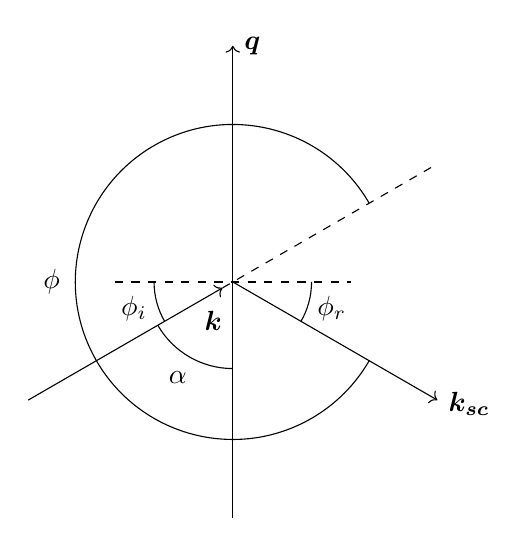
\begin{tikzpicture}

	% Draw wave vectors
	\draw[->] (0,-3) -- (0,3);
	\draw[->,rotate=30] (-3,0) -- (-0.15,0);
	\draw[->,rotate=-30] (0,0) -- (3,0);
	\draw (3,-1.55) node{$\bm{k_\mrm{sc}}$} (0.25,3) node{$\bm{q}$} (-0.25,-0.5) node{$\bm{k}$};
	
	% Draw dashed lines
	\draw[dashed,rotate=30] (-0.15,0) -- (3,0);
	\draw[dashed] (-1.5,0) -- (1.5,0);
	
	% Draw angles
	\draw ([shift={(30:2)}] 0,0) arc(30:330:2) (180:2.3) node{$\phi$};
	\draw ([shift={(-150:1.1)}] 0,0) arc(-150:-90:1.1) (-120:1.4) node{$\alpha$};
	\draw ([shift={(180:1)}] 0,0) arc(180:210:1) (195:1.3) node{$\phi_\mrm{i}$};
	\draw ([shift={(0:1)}] 0,0) arc(0:-30:1) (-15:1.3) node{$\phi_\mrm{r}$};
	
\end{tikzpicture}
			\caption{- case}
		\end{subfigure}
		\caption{\label{fig:bragg-comparison} Comparison of angles used in this model and angles of incidence and reflection. Both for the + and - cases.}
	\end{figure}

\subsection{Refined interaction region \label{sec:app-derivations-bragg-refined}}
For the refined interaction region described in section \ref{sec:app-derivations-refined} the derivation for finding a maximum scattering geometry is different than above. However, a first hypothesis would be that the resulting condition would be the same. To test this, the angles described by equations \eqref{eq:app-bragg-theta}, \eqref{eq:app-bragg-alpha}, \eqref{eq:app-bragg-phi} are inserted in $\Phi_\mrm{p}^{\pm}(\theta, \phi)$ from section \ref{sec:app-derivations-refined}. The function can be written as
\begin{equation*}
\begin{split}
	\Phi_\mrm{p}^{\pm}(\theta, \phi) &= \text{sinc}\left( \frac{d_\mrm{a}}{2\pi \sin{\alpha}}(k - k\sin{\theta}\cos{\phi} \pm q\cos{\alpha}) \right) \\
	&\cdot \text{sinc}\left( \frac{d_\mrm{e}}{2\pi \tan{\alpha}}
	(k - k\sin{\theta}(\cos{\phi} + \sin{\phi}\tan{\alpha}) \pm q(\cos{\alpha} + \sin{\alpha}\tan{\alpha})) \right) \\
	&\cdot \text{sinc}\left( -\frac{L_{z}}{2\pi} k\cos{\theta} \right)
\end{split}
\end{equation*}
As for the function used in derivations for the cuboid geometry, the maximum value of this function is 1. This happens only when the arguments of all sinc's are 0. Due to this fact, the problem is simplified by only considering the parts of the arguments required to be zero, namely
\begin{numcases}{}
	k - k\sin{\theta}\cos{\phi} \pm q\cos{\alpha} \label{eq:app-bragg-ref1} \\
	k - k\sin{\theta}(\cos{\phi} + \sin{\phi}\tan{\alpha}) \pm q(\cos{\alpha} + \sin{\alpha}\tan{\alpha} \label{eq:app-bragg-ref2} \\
	-\frac{L_{z}}{2\pi} k\cos{\theta} \label{eq:app-bragg-ref3}
\end{numcases}
Now the equations \eqref{eq:app-bragg-theta}, \eqref{eq:app-bragg-alpha}, \eqref{eq:app-bragg-phi} are inserted. In the derivations the following relations are well used
\begin{align*}
	\cos(\mp \pi + 2\alpha) &= \sin^2{\alpha} - \cos^2{\alpha} \\
	\sin(\mp \pi + 2\alpha) &= -2\sin{\alpha}\cos{\alpha} \\
	q &= \mp 2k\cos{\alpha}
\end{align*}
Argument \eqref{eq:app-bragg-ref1} is now written as
\begin{equation*}
\begin{split}
	k &- k\sin(\pi/2)\cos(\mp \pi + 2\alpha) \pm q\cos{\alpha} = k \left( 1 - (\sin^2{\alpha} - \cos^2{\alpha}) \pm (\mp 2\cos^2{\alpha}) \right) \\
	&= k \left( 1 - \sin^2{\alpha} - \cos^2{\alpha} \right) = 0
\end{split}
\end{equation*}
Since it is equal to zero, the first sinc is maximized. Now argument \eqref{eq:app-bragg-ref2} is written as
\begin{equation*}
\begin{split}
	k &- k\sin(\pi/2)(\cos(\mp \pi + 2\alpha) + \sin(\mp \pi + 2\alpha)\tan{\alpha}) \pm q(\cos{\alpha} + \sin{\alpha}\tan{\alpha} \\
	&= k \left( 1 - (\sin^2{\alpha} - \cos^2{\alpha} - 2\sin{\alpha}\cos{\alpha}\tan{\alpha}) \pm (\mp 2\cos{\alpha})(\cos{\alpha} + \sin{\alpha}\tan{\alpha}) \right) \\
	&= k \left( 1 - \sin^2{\alpha} + \cos^2{\alpha} + 2\sin^2{\alpha} - 2\cos^2{\alpha} - 2\sin^2{\alpha} \right) \\
	&= k \left( 1 - \sin^2{\alpha} - \cos^2{\alpha} \right) = 0
\end{split}
\end{equation*}
Since it is equal to zero, the second sinc is maximized. Finally, argument \eqref{eq:app-bragg-ref3} is written as
\begin{equation*}
	-\frac{L_{z}}{2\pi} k\cos{\pi/2} = 0
\end{equation*}
Since it is equal to zero, the third sinc is also maximized. Thus, all sinc functions are maximized which maximizes $\Phi_\mrm{p}^{\pm}$. This shows that the same condition (equations \eqref{eq:app-bragg-theta}, \eqref{eq:app-bragg-alpha}, \eqref{eq:app-bragg-phi}) maximizes the scattering for both the simple cuboid geometry and the refined geometry based on beams.
\todoint[inline]{Explain factor 1/sin(alpha) related to scattering volume and why this is not included in the maximization thing}
	
\end{document}